% PDF-A metadata
\begin{filecontents*}[overwrite]{\jobname.xmpdata}
  \Title{Models, algorithms and protocols for innovative deployment solutions in 5G and 6G cellular networks}
  \Author{Matteo Pagin}
  \Language{en-GB}
  \Subject{Thesis in partial fullfilment of the requirements for the PhD in Information Engineering of the Department of Information Engineering, University of Padova}
  \Keywords{5G\sep 6G\sep RIS\sep IAB}
\end{filecontents*}
  

\documentclass{mimosis}
\usepackage[a4paper]{geometry}
\geometry{left=1.55in}
\geometry{right=1.55in}
% PDF-A output
\usepackage{metalogo}
\usepackage[a-3u, mathxmp]{pdfx}

% Compile just one chapter
%\includeonly{Sources/chapter_to_include.tex}

%\DeclareUnicodeCharacter{0301}{*************************************}

%%%%%%%%%%%%%%%%%%%%%%%%%%%%%%%%%%%%%%%%%%%%%%%%%%%%%%%%%%%%%%%%%%%%%%%%
% Some of my favorite personal adjustments
%%%%%%%%%%%%%%%%%%%%%%%%%%%%%%%%%%%%%%%%%%%%%%%%%%%%%%%%%%%%%%%%%%%%%%%%
%
% These are the adjustments that I consider necessary for typesetting
% a nice thesis. However, they are *not* included in the template,   as
% I do not want to force you to use them.

% This ensures that I am able to typeset bold font in table while still aligning the numbers
% correctly.
\usepackage{etoolbox}

\usepackage{siunitx}
\DeclareSIUnit\px{px}
\DeclareSIUnit\dBm{dBm}

\sisetup{%
  detect-all           = true,
  detect-family        = true,
  detect-mode          = true,
  detect-shape         = true,
  detect-weight        = true
}

%%%%%%%%%%%%%%%%%%%%%%%%%%%%%%%%%%%%%%%%%%%%%%%%%%%%%%%%%%%%%%%%%%%%%%%%
% Customs 
%%%%%%%%%%%%%%%%%%%%%%%%%%%%%%%%%%%%%%%%%%%%%%%%%%%%%%%%%%%%%%%%%%%%%%%%


% Openright with oneside class
% Taken from http://mirrors.ctan.org/macros/latex/unpacked/latex.ltx
\makeatletter
\def\cleardoublepage{\clearpage\ifodd\c@page\else
    \hbox{}\newpage\if@twocolumn\hbox{}\newpage\fi\fi}
\makeatother

% List of publications highlighted name
\newcommand{\myself}{\textbf{\textcolor{UNIPDRED}{M. Pagin}}}
% Show publication list in ToC
\newcommand{\addchapterline}[1]{%
  \addcontentsline{toc}{chapter}{#1}%
}

% No footnote ends in different pages
\interfootnotelinepenalty=10000

\usepackage{amsthm}

% Algorithms
\usepackage{algpseudocode,algorithm,algorithmicx}
% Asymptotic computational complexity
\newcommand\bigO[1]{$\mathcal{O}(#1)$}

% Safehual commands and packages
\newcommand{\cvar}[1]{{\mathrm{CVaR}}_{#1}}
\newcommand{\estcvar}[1]{{\widehat{\mathrm{CVaR}}}_{#1}}
\newcommand{\ProbName}{MS\&RA}
\newcommand{\name}{Safehaul}
\newcommand{\donor}{BS-donor}
\newcommand{\donors}{BS-donors}
\newcommand{\node}{BS-node}
\newcommand{\nodes}{BS-nodes}
\newcommand\Algphase[1]{\vspace*{-.7\baselineskip}\Statex\hspace*{\dimexpr-\algorithmicindent-2pt\relax}\rule{\columnwidth}{0.4pt}\Statex\hspace*{-\algorithmicindent}\textbf{#1}\vspace*{-.7\baselineskip}\Statex\hspace*{\dimexpr-\algorithmicindent-2pt\relax}\rule{\columnwidth}{0.4pt}}
\renewcommand{\algorithmicrequire}{\textbf{Input:}}
\renewcommand{\algorithmicensure}{\textbf{Output:}}
\DeclareMathOperator{\ue}{ue}
\DeclareMathOperator{\size}{size}
\newcolumntype{L}[1]{>{\raggedright\let\newline\\\arraybackslash\hspace{0pt}}m{#1}}
\newcolumntype{C}[1]{>{\centering\let\newline\\\arraybackslash\hspace{0pt}}m{#1}}
\newcolumntype{R}[1]{>{\raggedleft\let\newline\\\arraybackslash\hspace{0pt}}m{#1}}
\newcommand{\fref}[1]{Fig.~\ref{#1}}
\usepackage{blkarray} 
\usepackage[export]{adjustbox} 
\usepackage{setspace}\usepackage{optidef}
\newtheorem{definition}{Definition}[]
\newtheorem{proposition}[definition]{Proposition}
\newtheorem{fact}[definition]{Fact}
\newtheorem{example}[definition]{Example}
\newtheorem{theorem}{Theorem}
\newtheorem{lemma}[definition]{Lemma}
\newtheorem{condition}[definition]{Condition}
\newtheorem{corollary}[definition]{Corollary}
\newtheorem{remark}[definition]{Remark}

% Irs clustering commands
\usepackage{IEEEtrantools}

%\usepackage{pgfplots,pgfplotstable}
%\usepgfplotslibrary{patchplots,groupplots}
%\usepackage{tikzscale}
\usepackage{tikz-qtree}
\usetikzlibrary{calc}

% bm commands
\usepackage{bm}
\usepackage{bbm}
% Lemma environment
%\newtheorem{thm}{Theorem}[section]
\newtheorem{lem}{Lemma}
% Better QED
\renewcommand\qedsymbol{$\blacksquare$}

\definecolor{UNIPDRED}{RGB}{155,0,20}

\setcounter{tocdepth}{3}
\setcounter{secnumdepth}{3}

% Coloured chapter numbers
\renewcommand*{\chapterformat}{%
 \selectfont\textcolor{UNIPDRED}{\huge\thechapter}\hspace{0.2in}%
}

\usepackage[inline]{enumitem}

% Spot error
% \DeclareUnicodeCharacter{0301}{*************************************}

% Better tables
\usepackage{colortbl}
\usepackage{multirow}
\usepackage{hhline}

\renewcommand\chapterlineswithprefixformat[3]{%
  \MakeUppercase{#2#3}
}

% Placeholder text
\usepackage{lipsum}

% TikZ & Co.
\usepackage{tikz}
\usepackage{pgfplots}
\pgfplotsset{compat=newest}
\usepgfplotslibrary{polar}
\usepackage{pgfplotstable}
\pgfplotsset{plot coordinates/math parser=false} 
\usetikzlibrary{plotmarks,patterns,positioning,patterns.meta,decorations.pathreplacing,backgrounds,calc,arrows,arrows.meta,spy,matrix}
\newlength\fheight
\newlength\fwidth
\usepackage{booktabs}
\usepackage{multirow}
\usepgfplotslibrary{patchplots,groupplots,patchplots,fillbetween}
\usepackage{tikzscale}
\def\si{\tikz\fill[scale=0.4](0,.35) -- (.25,0) -- (1,.7) -- (.25,.15) -- cycle;}

% Labels and tick default size
\pgfplotsset{every tick label/.append style={font=\footnotesize}}
\pgfplotsset{every axis/.append style={label style={font=\footnotesize}, tick label style={font=\footnotesize}}}
%\DeclareUnicodeCharacter{2212}{-} % TEMPORARY, just for TikZ

% Externalize TikZ figures
\usetikzlibrary{external}
\tikzexternalize[prefix=Cache/] % activate and define figures/ as cache folder

\usepackage{afterpage}
\usepackage{tabulary}

\usepackage{cuted} % strip environment
\usepackage{algpseudocode}

%%%%%%%%%%%%%%%%%%%%%%%%%%%%%%%%%%%%%%%%%%%%%%%%%%%%%%%%%%%%%%%%%%%%%%%%
% Hyperlinks & bookmarks
%%%%%%%%%%%%%%%%%%%%%%%%%%%%%%%%%%%%%%%%%%%%%%%%%%%%%%%%%%%%%%%%%%%%%%%%

\usepackage{bookmark}
\bookmarksetup{color=black}

%%%%%%%%%%%%%%%%%%%%%%%%%%%%%%%%%%%%%%%%%%%%%%%%%%%%%%%%%%%%%%%%%%%%%%%%
% Bibliography
%%%%%%%%%%%%%%%%%%%%%%%%%%%%%%%%%%%%%%%%%%%%%%%%%%%%%%%%%%%%%%%%%%%%%%%%
%
% I like the bibliography to be extremely plain, showing only a numeric
% identifier and citing everything in simple brackets. The first names,
% if present, will be initialized. DOIs and URLs will be preserved.

\usepackage[%
  autocite     = plain,
  backend      = biber,
  doi          = false,
  url          = false,
  giveninits   = true,
  hyperref     = true,
  maxbibnames  = 99,
  maxcitenames = 99,
  sorting		= none,
  style        = numeric-comp,
  ]{biblatex}
\hypersetup{
  % Document-wide hyperlinks color
  colorlinks=true,
  citecolor=UNIPDRED,
  linkcolor=UNIPDRED
  %allbordercolors=UNIPDRED
}
  
 \usepackage{xurl}

\addbibresource{Sources/bibl.bib}

%%%%%%%%%%%%%%%%%%%%%%%%%%%%%%%%%%%%%%%%%%%%%%%%%%%%%%%%%%%%%%%%%%%%%%%%
% Fonts
%%%%%%%%%%%%%%%%%%%%%%%%%%%%%%%%%%%%%%%%%%%%%%%%%%%%%%%%%%%%%%%%%%%%%%%%

%\usepackage[lf]{ebgaramond}
%\usepackage[scale=0.8]{sourcecodepro}
%\usepackage{newpxtext,newpxmath} % Palatino like text and math
%\sffamily%

\IfFileExists{mathpazo.sty}{\RequirePackage[osf,sc]{mathpazo}}{}
\IfFileExists{helvet.sty}{\RequirePackage[scaled=0.90]{helvet}}{}
\IfFileExists{beramono.sty}{\RequirePackage[scaled=0.85]{beramono}}{}
\onehalfspacing

\renewcommand{\th}{\textsuperscript{\textup{th}}\xspace}

\newacronym{3gpp}{3GPP}{3rd Generation Partnership Project}
\newacronym{adc}{ADC}{Analog to Digital Converter}
\newacronym{afbw}{AFBW}{Average Fading Bandwidth}
\newacronym{5g}{5G}{5th generation}
\newacronym{4g}{4G}{4th generation}
\newacronym{aimd}{AIMD}{Additive Increase Multiplicative Decrease}
\newacronym{am}{AM}{Acknowledged Mode}
\newacronym{amf}{AMF}{Access and Mobility Management Function}
\newacronym{an}{AN}{Access Network}
\newacronym{amc}{AMC}{Adaptive Modulation and Coding}
\newacronym{aqm}{AQM}{Active Queue Management}
\newacronym{awgn}{AGWN}{Additive White Gaussian Noise}
\newacronym{balia}{BALIA}{Balanced Link Adaptation}
\newacronym{bsr}{BSR}{Buffer Status Report}
\newacronym{msr}{MSR}{Max Sum-Rate}
\newacronym{ba}{BA}{Backlog Avoidance}
\newacronym{mrba}{MRBA}{Max-Rate Backlog Avoidance}
\newacronym{bdp}{BDP}{Bandwidth-Delay Product}
\newacronym{bf}{BF}{Beamforming}
\newacronym{v2x}{V2X}{Vehicle-to-Everything}
\newacronym{vr}{VR}{Virtual Reality}
\newacronym{mdp}{MDP}{Markov Decision Process}
\newacronym{mwm}{MWM}{Maximum Weighted Matching}
\newacronym{tdm}{TDM}{Time Division Multiplexing}
\newacronym{fdm}{FDM}{Frequency Division Multiplexing}
\newacronym{sdm}{SDM}{Space Division Multiplexing}
\newacronym{st}{ST}{Spanning Tree}
\newacronym{rl}{RL}{Reinforcement Learning}
\newacronym{lp}{LP}{Linear Programming}
\newacronym[firstplural=Deep Neural Networks (DNNs)]{dnn}{DNN}{Deep Neural Network}
\newacronym{dag}{DAG}{Directed Acyclic Graph}
\newacronym{gtp}{GTP}{GPRS Tunneling Protocol}
\newacronym{nas}{NAS}{Non-Access Stratum}
\newacronym{isp}{ISP}{Internet Service Provider}
\newacronym{ngnm}{NGNM}{Next Generation Mobile Networks Alliance}
\newacronym{cc}{CC}{Component Carrier}
\newacronym{drb}{DRB}{Data Radio Bearer}
\newacronym{qos}{QoS}{Quality of Service}
\newacronym{ca}{CA}{Carrier Aggregation}
\newacronym{sdap}{SDAP}{Service Data Adaptation Protocol}
\newacronym{lc}{LC}{Logical Channel}
\newacronym{rnti}{RNTI}{Radio Network Temporary Identifier}
\newacronym{qci}{QCI}{Quality Class Identifier}
\newacronym{cdf}{CDF}{Cumulative Distribution Function}
\newacronym{cmos}{CMOS}{Complementary Metal-Oxide Semiconductor}
\newacronym{cn}{CN}{Core Network}
\newacronym{cqi}{CQI}{Channel Quality Information}
\newacronym{cir}{CIR}{Channel Impulse Response}
\newacronym{cp}{CP}{Control Plane}
\newacronym{cu}{CU}{Central Unit}
\newacronym{du}{DU}{Distributed Unit}
\newacronym{csirs}{CSI-RS}{Channel State Information - Reference Signal}
\newacronym{dc}{DC}{Dual Connectivity}
\newacronym{imsi}{IMSI}{International Mobile Subscriber Identity}
\newacronym{dce}{DCE}{Direct Code Execution}
\newacronym{dci}{DCI}{Downlink Control Information}
\newacronym{uci}{UCI}{Uplink Control Information}
\newacronym{dl}{DL}{Downlink}
\newacronym{dmr}{DMR}{Deadline Miss Ratio}
\newacronym{dmrs}{DMRS}{DeModulation Reference Signal}
\newacronym{e2e}{E2E}{End-to-End}
\newacronym{ecn}{ECN}{Explicit Congestion Notification}
\newacronym{edf}{EDF}{Earliest Deadline First}
\newacronym{enb}{eNB}{evolved Node Base}
\newacronym{embb}{eMBB}{enhanced Mobile Broadband}
\newacronym{epc}{EPC}{Evolved Packet Core}
\newacronym{es}{ES}{Edge Server}
\newacronym{fdma}{FDMA}{Frequency Division Multiple Access}
\newacronym{fdd}{FDD}{Frequency Division Duplexing}
\newacronym[firstplural=Radio Access Technologies (RATs)]{rat}{RAT}{Radio Access Technology}
\newacronym[firstplural=Markov Chains (MCs)]{mc}{MC}{Markov Chain}
\newacronym{milp}{MILP}{Mixed-Integer Linear Programming}
\newacronym{fs}{FS}{Fast Switching}
\newacronym{ip}{IP}{Internet Protocol}
\newacronym{fr}{FR}{Frequency Range}
\newacronym{ftp}{FTP}{File Transfer Protocol}
\newacronym{gnb}{gNB}{Next Generation Node Base}
\newacronym{arq}{ARQ}{Automatic Repeat reQuest}
\newacronym{harq}{HARQ}{Hybrid Automatic Repeat reQuest}
\newacronym{hetnet}{HetNet}{Heterogeneous Network}
\newacronym{hh}{HH}{Hard Handover}
\newacronym{hol}{HOL}{Head-of-Line}
\newacronym{ia}{IA}{Initial Access}
\newacronym{imt}{IMT}{International Mobile Telecommunication}
\newacronym{iot}{IoT}{Internet of Things}
\newacronym{lcr}{LCR}{Level Crossing Rate}
\newacronym{lcf}{LCF}{Level Crossing Frequency}
\newacronym{los}{LoS}{Line-of-Sight}
\newacronym{lte}{LTE}{Long Term Evolution}
\newacronym{m2m}{M2M}{Machine to Machine}
\newacronym{mac}{MAC}{Medium Access Control}
\newacronym{num}{NUM}{Network Utility Maximization}
\newacronym{ri}{RI}{Rank Index}
\newacronym{pmi}{PMI}{Precoding Matrix Index}
\newacronym{mcs}{MCS}{Modulation and Coding Scheme}
\newacronym{mec}{MEC}{Mobile Edge Cloud}
\newacronym{mi}{MI}{Mutual Information}
\newacronym{mimo}{MIMO}{Multiple Input, Multiple Output}
\newacronym{mmwave}{mmWave}{millimeter wave}
\newacronym{mptcp}{MPTCP}{Multipath TCP}
\newacronym{mr}{MR}{Maximum Rate}
\newacronym{mt}{MT}{Mobile Termination}
\newacronym{mss}{MSS}{Maximum Segment Size}
\newacronym{mtd}{MTD}{Machine-Type Device}
\newacronym{mtu}{MTU}{Maximum Transmission Unit}
\newacronym{nfv}{NFV}{Network Function Virtualization}
\newacronym{nf}{NF}{Network Function}
\newacronym{nlos}{NLoS}{Non-Line-of-Sight}
\newacronym{nr}{NR}{New Radio}
\newacronym{csi}{CSI}{Channel State Information}
\newacronym{o2i}{O2I}{Outdoor-to-Indoor}
\newacronym{ofdm}{OFDM}{Orthogonal Frequency Division Multiplexing}
\newacronym{pdcch}{PDCCH}{Physical Downlink Control Channel}
\newacronym{pdcp}{PDCP}{Packet-Data Convergence Protocol}
\newacronym{pdsch}{PDSCH}{Physical Downlink Shared Channel}
\newacronym{pdu}{PDU}{Packet Data Unit}
\newacronym{sdu}{SDU}{Service Data Unit}
\newacronym{pf}{PF}{Proportional Fair}
\newacronym{pgw}{PGW}{Packet Gateway}
\newacronym{phy}{PHY}{Physical}
\newacronym{pbch}{PBCH}{Physical Broadcast Channel}
\newacronym[plural=\gls{mme}s,firstplural=Mobility Management Entities (MMEs)]{mme}{MME}{Mobility Management Entity}
\newacronym{prb}{PRB}{Physical Resource Block}
\newacronym{pss}{PSS}{Primary Synchronization Signal}
\newacronym{pucch}{PUCCH}{Physical Uplink Control Channel}
\newacronym{pusch}{PUSCH}{Physical Uplink Shared Channel}
\newacronym{rach}{RACH}{Random Access Channel}
\newacronym{ran}{RAN}{Radio Access Network}
\newacronym{ngran}{NG-RAN}{Next Generation RAN}
\newacronym{red}{RED}{Random Early Detection}
\newacronym{rf}{RF}{Radio Frequency}
\newacronym{rlc}{RLC}{Radio Link Control}
\newacronym{rlf}{RLF}{Radio Link Failure}
\newacronym{rrc}{RRC}{Radio Resource Control}
\newacronym{rrm}{RRM}{Radio Resource Management}
\newacronym{rr}{RR}{Round Robin}
\newacronym{rs}{RS}{Remote Server}
\newacronym{rsrp}{RSRP}{Reference Signal Received Power}
\newacronym{rss}{RSS}{Received Signal Strength}
\newacronym{rtt}{RTT}{Round Trip Time}
\newacronym{rw}{RW}{Receive Window}
\newacronym{rx}{RX}{Receiver}
\newacronym{sa}{SA}{standalone}
\newacronym{sack}{SACK}{Selective Acknowledgment}
\newacronym{sap}{SAP}{Service Access Point}
\newacronym{sch}{SCH}{Secondary Cell Handover}
\newacronym{scoot}{SCOOT}{Split Cycle Offset Optimization Technique}
\newacronym{sdma}{SDMA}{Spatial Division Multiple Access}
\newacronym{sdn}{SDN}{Software Defined Networking}
\newacronym{sinr}{SINR}{Signal-to-Interference-plus-Noise Ratio}
\newacronym{sir}{SIR}{Signal-to-Interference Ratio}
\newacronym{sm}{SM}{Saturation Mode}
\newacronym{snr}{SNR}{Signal-to-Noise Ratio}
\newacronym{son}{SON}{Self-Organizing Network}
\newacronym{ss}{SS}{Synchronization Signal}
\newacronym{srs}{SRS}{Sounding Reference Signal}
\newacronym{sss}{SSS}{Secondary Synchronization Signal}
\newacronym{tb}{TB}{Transport Block}
\newacronym{tcp}{TCP}{Transmission Control Protocol}
\newacronym{tdd}{TDD}{Time Division Duplexing}
\newacronym{tdma}{TDMA}{Time Division Multiple Access}
\newacronym{tfl}{TfL}{Transport for London}
\newacronym{tm}{TM}{Transparent Mode}
\newacronym{trp}{TRP}{Transmitter Receiver Pair}
\newacronym{tti}{TTI}{Transmission Time Interval}
\newacronym{ttt}{TTT}{Time-to-Trigger}
\newacronym{tx}{TX}{Transmitter}
\newacronym{qam}{QAM}{Quadrature Amplitude Modulation}
\newacronym{ue}{UE}{User Equipment}
\newacronym{ul}{UL}{Uplink}
\newacronym{uml}{UML}{Unified Modeling Language}
\newacronym{um}{UM}{Unacknowledged Mode}
\newacronym{uma}{UMa}{Urban Macro}
\newacronym{utc}{UTC}{Urban Traffic Control}
\newacronym{vm}{VM}{Virtual Machine}
\newacronym{rsrq}{RSRQ}{Reference Signal Received Quality}
\newacronym{rssi}{RSSI}{Received Signal Strength Indicator}
\newacronym{crs}{CRS}{Cell Reference Signal}
\newacronym{nsa}{NSA}{Non Stand Alone}
\newacronym{mrdc}{MR-DC}{Multi \gls{rat} \gls{dc}}
\newacronym{eutra}{E-UTRA}{Evolved Universal Terrestrial Radio Access}
\newacronym{endc}{EN-DC}{E-UTRAN-\gls{nr} \gls{dc}}
\newacronym{5gc}{5GC}{5G Core}
\newacronym{si}{SI}{Study Item}
\newacronym{iab}{IAB}{Integrated Access and Backhaul}
\newacronym{wf}{WF}{Wired-first}
\newacronym{hqf}{HQF}{Highest-quality-first}
\newacronym{pa}{PA}{Position-aware}
\newacronym{mlr}{MLR}{Maximum-local-rate}
\newacronym{wbf}{WBF}{Wired Bias Function}
\newacronym{mib}{MIB}{Master Information Block}
\newacronym{sib}{SIB}{Secondary Information Block}
\newacronym{kpi}{KPI}{Key Performance Indicator}
\newacronym{ppp}{PPP}{Poisson Point Process}
\newacronym{mpc}{MPC}{Multi Path Component}
\newacronym{rt}{RT}{Ray Tracer}
\newacronym{aoa}{AoA}{Angle of Arrival}
\newacronym{aod}{AoD}{Angle of Departure}
\newacronym{scm}{SCM}{Spatial Channel Model}
\newacronym{inr}{INR}{Interference to Noise Ratio}
\newacronym{qd}{QD}{Quasi Deterministic}
\newacronym{wlan}{WLAN}{Wireless Local Area Network}
\newacronym{cad}{CAD}{Computer-aided Design}
\newacronym{ap}{AP}{Access Point}
\newacronym{sta}{STA}{Station}
\newacronym{urllc}{URLLC}{Ultra-Reliable Low-Latency Communication}
\newacronym{udp}{UDP}{User Datagram Protocol}
\newacronym{upf}{UPF}{User Plane Function}
\newacronym{umi}{UMi}{Urban Microcell}
\newacronym{uma2}{UMa}{Urban Macrocell}
\newacronym{rma}{RMa}{Rural Macrocell}
\newacronym{in}{In}{Indoor Office}
\newacronym{wpans}{WPANs}{Wireless Personal Area Networks}
\newacronym{wpan}{WPAN}{Wireless Personal Area Network}
\newacronym{fd}{FD}{Full Duplex}
\newacronym{crc}{CRC}{Cyclic Redundancy Check}
\newacronym{wb}{WB}{Wideband}
\newacronym{sb}{SB}{Subband}
\newacronym{bap}{BAP}{Backhaul Adaptation Protocol}
\newacronym{lcg}{LCG}{Logical Channel Group}
\newacronym{ecdf}{ECDF}{Empirical Cumulative Distribution Function}
\newacronym{mu}{MU}{Multi-User}
\newacronym{ce}{CE}{Control Element}
\newacronym{ric}{RIC}{RAN Intelligent Controller}
\newacronym{bler}{BLER}{Block Error Rate}
\newacronym{ieee}{IEEE}{Institute of Electrical and Electronics Engineers}
\newacronym{ilp}{ILP}{Integer Linear Program}
\newacronym{ldpc}{LDPC}{Low-Density Parity Check}
\newacronym{nlosv}{NLOSv}{Vehicle Non-Line-of-Sight}
\newacronym{pscch}{PSCCH}{Physical Sidelink Control Channel}
\newacronym{sc}{SC}{Single Carrier}
\newacronym{sl}{SL}{Sidelink}
\newacronym{dft}{DFT}{Discrete Fourier Transform}
\newacronym{v2v}{V2V}{Vehicle-to-Vehicle}
\newacronym{wave}{WAVE}{Wireless Access in Vehicular Environments}
\newacronym{upa}{UPA}{Uniform Planar Array}
\newacronym{fec}{FEC}{Forward Error Correction}
\newacronym{psfch}{PSFCH}{Physical Sidelink Feedback Channel}
\newacronym{pssch}{PSSCH}{Physical Sidelink Shared Channel}
\newacronym{csma}{CSMA}{Carrier Sense Multiple Access}
\newacronym{v2n}{V2N}{Vehicle-to-Network}
\newacronym{cav}{CAV}{Connected and Autonomous Vehicle}
\newacronym{v2i}{V2I}{Vehicle-to-Infrastructure}
\newacronym{d2d}{D2D}{Device-to-Device}
\newacronym{c-its}{C-ITS}{Connected Intelligent Transportation System}
\newacronym{fr2}{FR2}{Frequency Range 2}
\newacronym{bs}{BS}{Base Station}
\newacronym{scs}{SCS}{Subcarrier Spacing}
\newacronym{sumo}{SUMO}{Simulation of Urban MObility}
\newacronym{prr}{PRR}{Packet Reception Ratio}
\newacronym{edca}{EDCA}{Enhanced Distribution Channel Access}
\newacronym{thz}{THz}{terahertz}
\newacronym{6g}{6G}{6th generation}
\newacronym{uav}{UAV}{unmanned aerial vehicles}

\makeindex
\makeglossaries

%%%%%%%%%%%%%%%%%%%%%%%%%%%%%%%%%%%%%%%%%%%%%%%%%%%%%%%%%%%%%%%%%%%%%%%%
% Incipit
%%%%%%%%%%%%%%%%%%%%%%%%%%%%%%%%%%%%%%%%%%%%%%%%%%%%%%%%%%%%%%%%%%%%%%%%

\title{\textcolor{UNIPDRED}{Models, algorithms\\[0.2cm] and protocols for\\[0.2cm] innovative deployment\\[0.2cm] solutions in 5G and 6G\\[0.2cm] cellular networks}}
\author{Matteo Pagin}

\begin{document}

\frontmatter
  \begin{titlepage}
  \makeatletter

  %\begin{figure}
  %  \centering
  %  \includegraphics[width=0.4\textwidth]{unipd_logo_and_text.pdf}
  %\end{figure}
  %\vspace*{1cm}
  {
    \sffamily%
    \fontsize{20}{24}\selectfont\par\noindent\textcolor{black}{\MakeUppercase{\@author}}%
    \vspace*{1cm}%
    \fontsize{24}{46}\selectfont\par\noindent{\MakeUppercase{\@title}}%
  }

  \vspace{1.5cm}
  {
    \begin{center}
      
\includegraphics[width=5cm]{Figures/unipd_logo_only.pdf}
    \end{center}
  }

  \vspace{1.5cm}
  {
    \sffamily%
    \fontsize{8}{15}\selectfont\par\noindent\textcolor{black}
    {\MakeUppercase{A thesis submitted in partial fulfillment of the requirements for the}}
    \vspace{0.1cm}%
    \fontsize{12}{15}\selectfont\par\noindent\textcolor{black}
    {\MakeUppercase{Ph.D. Degree in Information Engineering}}
    \vspace{0.1cm}%
    \fontsize{8}{15}\selectfont\par\noindent\textcolor{black}
    {\MakeUppercase{of the}}
    \vspace{0.1cm}
    \fontsize{12}{15}\selectfont\par\noindent\textcolor{black}
    {\MakeUppercase{Department of Information Engineering\\University of Padova}}%
    \vspace{0.1cm}%
    \fontsize{8}{15}\selectfont\par\noindent\textcolor{black}
    {\MakeUppercase{supervised by}}
    \vspace{0.1cm}%
    \fontsize{12}{15}\selectfont\par\noindent\textcolor{black}
    {\MakeUppercase{prof. Michele Zorzi}}%
  }

  \vspace*{\fill}
  {
    \sffamily%
    \fontsize{12}{15}\selectfont\par\noindent{\MakeUppercase{XXXVII Cycle}}%
    \fontsize{12}{15}\selectfont\par\noindent{\MakeUppercase{Academic year 2023/2024}}%
    % \fontsize{8}{10}\selectfont\par\noindent{\MakeUppercase{Graduation date XXXX}}%
  }
  \makeatother
\end{titlepage}

\newpage
\null
\thispagestyle{empty}
\newpage

  {\noindent\huge\itshape Abstract}\\
%

Cellular networks are constantly evolving in order to support the ever-increasing number of mobile users, and the corresponding growth in wireless data traffic, coupled with the emergence of new applications. 
Specifically, the last iteration of mobile networks, i.e., 5G, brought high peak performance and extreme flexibility, making it possible to support a diverse set of applications with heterogeneous yet stringent requirements. 
One of 5G main novelties is represented by the support for \gls{mmwave} frequencies, which unlocks an unprecedented amount of previously unused radio resources. In turn, the latter enables extremely high data rates and low latencies. Moreover, it is envisioned that the upcoming generation, i.e., 6G, will unleash additional bandwidth, by further expanding the supported spectrum bands to include \gls{thz} frequencies as well. 
However, despite their theoretical potential, \gls{mmwave} and \gls{thz} frequencies exhibit harsh propagation conditions which make it challenging to provide ubiquitous high speed wireless connectivity. 
To fill this gap, this thesis studies innovative deployment solutions to overcome the unfavorable propagation characteristics of \gls{mmwave} and \gls{thz} communications, paving the way for their widespread use in the context of 6G cellular networks. 

In particular, this thesis
\begin{enumerate*}[label=(\roman*)]
    \item presents novel simulation tools, which model innovative coverage enhancement technologies such as \glspl{irs}, \gls{af} relays, and \glspl{ntn};
    \item presents novel simulation models which improve the computational complexity of \gls{mimo} simulations;
    \item introduces schemes for optimizing \gls{iab} networks;
    \item analyzes the potential of mixed \gls{mmwave} and \gls{thz} links for wireless backhauling; and
    \item analyzes the impact of non-ideal control channels in \gls{irs}-aided deployments, and introduces algorithms for mitigating the corresponding performance degradation.
\end{enumerate*}

This thesis adopts a system-level approach, thus characterizing the network behavior in an end-to-end fashion, and capturing the interplay between the physical signal propagation and the different layers of the communications protocol stack. Results demonstrate the effectiveness of the proposed solutions, which pave the way towards ubiquitous high-performance mobile networks.
  {\noindent\huge\itshape Sommario}\\
%

% Cellular networks are constantly evolving in order to support the ever-increasing number of mobile users, and the corresponding growth in wireless data traffic, coupled with the emergence of new applications. 
% Specifically, the last iteration of mobile networks, i.e., 5G, brought high peak performance and extreme flexibility, making it possible to support a diverse set of applications with heterogeneous yet stringent requirements. 
Le reti cellulari sono in constante evoluzione, sia per sostenere il numero crescente di utenti mobili e la corrispondente crescita del traffico di dati, sia per far fronte all'emergenza di nuovi scenari d'uso.
In particolare, l'ultima versione delle reti mobili, ovvero 5G, offre alte prestazioni di picco ed estrema flessibilità, permettendo di sostenere un diverso insieme di applicazioni con caratteristiche eterogenee.
% One of 5G main novelties is represented by the support for \gls{mmwave} frequencies, which unlocks an unprecedented amount of previously unused radio resources. In turn, the latter enables extremely high data rates and low latencies. Moreover, it is envisioned that the upcoming generation, i.e., 6G, will unleash additional bandwidth, by further expanding the supported spectrum bands to include \gls{thz} frequencies as well. 
Una delle principali novità della tecnologia 5G è rappresentata dal supporto alle frequenze \gls{mmwave}, che forniscono l'accesso ad una quantità senza precedenti di risorse radio precedentemente non utilizzate. Queste ultime consentono trasmissioni dati a velocità estremamente elevate e latenze particolarmente basse. 
Inoltre, si prevede che la prossima generazione di reti cellulari, ovvero 6G, supporterà ulteriori bande includendo anche le frequenze \gls{thz}.

% However, despite their theoretical potential, \gls{mmwave} and \gls{thz} frequencies exhibit harsh propagation conditions which make it challenging to provide ubiquitous high speed wireless connectivity. 
% To fill this gap, this thesis studies innovative deployment solutions to overcome the unfavorable propagation characteristics of mmWave and THz communications, paving the way for their widespread use in the context of 6G cellular networks. 
Tuttavia, nonostante il loro potenziale teorico, le frequenze \gls{mmwave} e \gls{thz} presentano condizioni di propagazione estremamente sfavorevoli, che rendono difficile fornire una connessione wireless veloce ed onnipresente. 
A questo fine, questa tesi studia infrastrutture innovative per ovviare all'intrinsica limitata copertura delle comunicazioni mmWave e THz, aprendo la strada ad un loro utilizzo diffuso nel contesto delle reti cellulari 6G.

% In particular, this thesis
% \begin{enumerate*}[label=(\roman*)]
%     \item presents novel simulation tools, which model innovative coverage enhancement technologies such as \glspl{irs}, \gls{af} relays, and \glspl{ntn};
%     \item presents novel simulation models which improve the computational complexity of \gls{mimo} simulations;
%     \item introduces schemes for optimizing \gls{iab} networks;
%     \item analyzes the potential of mixed \gls{mmwave} and \gls{thz} links for wireless backhauling; and
%     \item analyzes the impact of non-ideal control channels in \gls{irs}-aided deployments, and introduces algorithms for mitigating the corresponding perofrmance degradation
% \end{enumerate*}.
In particolare, questa tesi
\begin{enumerate*}[label=(\roman*)]
\item presenta nuovi strumenti di simulazione, che modellano tecnologie di miglioramento della copertura innovative come \glspl{irs}, ripetitori \gls{af} e \glspl{ntn};
\item presenta nuovi modelli di simulazione che migliorano la complessità computazionale delle simulazioni \gls{mimo};
\item introduce schemi di ottimizzazione per reti \gls{iab};
\item analizza il potenziale di collegamenti misti \gls{mmwave} e \gls{thz} per wireless backhauling;
\item analizza l'impatto di canali di controllo non ideali in reti supportate da \glspl{irs} e introduce algoritmi per mitigare la conseguente perdita di prestazioni
\end{enumerate*}.

% This thesis adopts a system-level approach, thus characterizing the network behavior in an end-to-end fashion, and capturing the interplay between the physical signal propagation and the different layers of the communications protocol stack. Results demonstrate the effectiveness of the proposed solutions, which pave the way towards ubiquitous high-performance mobile networks.
Questa tesi adotta un approccio di studio a livello di sistema, quindi caratterizzando il comportamento della rete nel suo complesso e catturando l'interazione tra la propagazione del segnale fisico ed i diverse livelli dello stack protocollare. I risultati presentati dimostrano l'efficacia delle soluzioni proposte, che aprono quindi la strada verso reti cellulari di alte prestazione ubique.
  \newpage\phantom{justskipthepage}

{
  % Custom link color for TOC
  \hypersetup{linkcolor=black}
  \tableofcontents
}

\mainmatter
  %%%%%%%%%%%%%%%%%%%%%%%%%%%%%%%%%%%%%%%%%%%%%%%%%%%%%%%%%%%%%%%%%%%%%%%%
\chapter{Introduction}
%%%%%%%%%%%%%%%%%%%%%%%%%%%%%%%%%%%%%%%%%%%%%%%%%%%%%%%%%%%%%%%%%%%%%%%%

The significance of mobile networks in modern society is underscored by their paramount role in facilitating social, professional, and educational interactions. The recent COVID-19 pandemic has served as a bitter reminder of this critical importance, identifying the absence of Internet connectivity as a significant hindrance to our daily lives.
However, the current generation of cellular networks, i.e., \gls{5g}, are found wanting in providing adequate broadband coverage to rural regions~\cite{yaacoub2020key}. Furthermore, even in technologically advanced nations, cellular infrastructures often fall short of meeting the stringent reliability, availability, and responsiveness requirements of emerging wireless applications. The vulnerability of mobile networks to natural disasters and cyberattacks underscores the need for solutions which offer reliability from both a technological and a sociopolitical standpoint.
Indeed, recent geopolitical turmoils have expanded the scope of conflict to include the cyberspace, emphasizing the imperative of maintaining uninterrupted connectivity in emergency situations. In these contexts, connectivity outages can compromise the delivery of critical services, inflict significant economic damage, and even result in loss of lives~\cite{internet_ukr_afg}.

In response to the pressing need for reliable wireless connectivity, the \gls{itu} foresees a future where ubiquitous broadband coverage will be achieved by 2030. This vision is driven by the imperative to provide seamless connectivity to both humans and an increasingly vast array of intelligent devices, including wearables, autonomous vehicles, \glspl{uas}, and robots~\cite{mozaffari2018beyond}.
The advent of novel use cases such as holographic communications, \gls{xr}, and tactile applications will further exacerbate the requirements for peak throughput and latency identified for the 5G's \gls{embb} and \gls{urllc} use cases. 
To achieve these ambitions goals, future cellular systems will continue to evolve and enhance the 5G network paradigm, which has revolutionized the wireless landscape by introducing flexible virtualized architectures, the support for \gls{mmwave} communications, and the adoption of \gls{mimo} technologies~\cite{ghosh20195g}. 
Notably, both academic and industry researchers are exploring a more central role for \gls{mmwave} technology, with plans to allocate additional spectrum towards the \gls{thz} band, and the design of \gls{ai}-native networks, with the goal of achieving autonomous data-centric orchestration and management of the network~\cite{polese20216g}, possibly down to the air interface~\cite{hoydis2021toward}.
By harnessing the power of \gls{ai} and advanced wireless technologies, future cellular systems will be capable of self-organizing, self-healing, and self-adapt to ever-changing environments.

The THz and mmWave frequency bands hold significant promise as a means to achieve peak data rates exceeding Tb/s, as envisioned by the ITU~\cite{imt2030}. However, this portion of the spectrum is hampered by unfavorable propagation characteristics that make it challenging to realize its full potential.
Specifically, the THz and mmWave bands are plagued by a pronounced free-space propagation loss, which significantly attenuates signal strength over long distances. Furthermore, these frequencies are also susceptible to blockages, for instance due to buildings, foliage, and other obstacles, which can cause significant signal attenuation~\cite{han2018propagation, jornet2011channel}.
With 5G, preliminary support for \gls{mmwave} bands has been introduced thanks to a major redesign not only of the physical layer, but of the whole cellular protocol stack~\cite{shafi2018microwave}. For instance, the intrinsic directionality of the communication requires ad hoc control procedures~\cite{heng2021six}, while the frequent transitions between \gls{los} and \gls{nlos} conditions call for an ad hoc transport layer design, such as novel \gls{tcp} algorithms~\cite{zhang2019will}. 
Despite the harsh propagation environment can be partially mitigated by using directional links and densifying network deployments~\cite{polese2020toward}, these unfavorable propagation characteristics pose a significant challenge to the successful deployment of THz and mmWave-based wireless systems. Indeed, traditional network densification is costly for network operators,
especially in terms of sites acquisition campaigns, rental fees, and fiber optic layout to provide wired backhauling~\cite{lopez2015towards}.

To solve this issue, the 3GPP approved, as part of its 5G NR specifications for Rel-16~\cite{3gpp_38_874}, \gls{iab} as a new paradigm to replace fiber-like infrastructures with self-configuring relays operating through wireless backhaul links. However, while lower than that of wired backhaul deployments, the CAPEX costs of \gls{iab} installation may still prove prohibitive for \glspl{mno} [6].
In light of this, new technologies based on \glspl{irs} and \gls{af} relays are also emerging as promising alternatives to overcome the coverage issues of mmWave networks with energy and cost efficiency in mind.

TODO: talk about open, virtual and geopolitical impact.
In addition, as the network progressively becomes increasingly complex and heterogeneous, the push for spectrum expansion will be coupled with an \gls{ai}-native design which, thanks to the ongoing virtualization, will not be limited to the radio link level, but will encompass the orchestration of large scale deployments as well~\cite{polese2023understanding}.
Nevertheless, how to design, test and eventually deploy management and orchestration algorithms is an open research challenge~\cite{polese2022colo}.
First, the training data must accurately capture the interplay of the whole protocol stack with the wireless channel. Furthermore, optimization frameworks such as \gls{drl} also call for preliminary testing in isolated yet realistic environments, with the goal of minimizing the performance degradation to actual network deployments~\cite{lacava2022programmable, amir2023safehaul}.


% To enable these new scenarios, there is the need to optimize different aspects of the communi-
% cation workflow, from a thorough characterization of the applications of interest (e.g., to better
% understand how to schedule resources based on the tra\ufb00ic sources) to the precise modeling of
% the signal propagation. Still, during these years, the general lack of a proper instrumentation
% to accurately test new solutions on real-word testbeds (usually related to the prohibitive cost
% of hardware operating at mmWave, jointly with the difficulty of implementing solutions on
% scenarios as difficult as the automotive one), further slowed down the go-to-market of mmWave-
% capable devices. Fortunately, thanks to increasingly precise simulation tools (such as Network
% Simulator 2 (ns-2) [13], Network Simulator 3 (ns-3) [14], OMNeT++ [15], etc.), the hardware
% availability might turn fundamental only in the final steps of the study, to assess the best so-
% lutions chosen from those studied through extensive simulations. Among the main features of
% ns-3, one of the main research tools used to obtain the results discussed in this thesis, its mod-
% ularity allows researchers to create solutions completely from scratch, as well as add features
% on modules openly available and that have been thoroughly used and tested by the community.
% An example consists of ns3-mmwave [16], a 5G-NR-compliant and openly available module [17],
% that allows the simulation of next-generation networks operating at mmWave.
% It has also to be acknowledged that, in the recent years, there has been an effort from gov-
% ernment agencies all over the world to create fundings opportunities for research institutions
% to support the creation of public platforms to carry out advanced research in wireless com-
% munications, to fill the gap described above. An example consists in the US-based Plaftorms
% for Advanced Wireless Research (PAWR) initiative, a $100$ million partnership funded by the
% National Science Foundation (NSF) and a consortium of 30 companies and associations, for the
% creation of 4 city-scale research testbeds [18]. The European Union, instead, to combat the
% negative impact of COVID-19, agreed to invest together €750 billion (in 2018 prices) to build a
% greener, more digital and more resilient Europe. Part of these funds has already been allocated
% towards research and innovation, which will use it, among other things, to sustain the costs of
% top-notch instrumentation and open hardware facilities [19].
% To sum up, in this dissertation, besides giving a detailed overview of the aforementioned
% problems, we contribute to the state of the art with improvements that span from the creation
% of novel ns-3 modules, to the design of artificial intelligence algorithms to proactively assist
% teleoperated driving operations, to the setup of a reproducible workflow for carrying out end-
% to-end measurements on a public platform for wireless research. Even though we touched on
% very diverse topics, from indoor network operations for XR applications to intelligent vehicular
% networks, they were all connected by the interest in studying and evaluating different technolo-
% gies that make up the next generation of mobile networks. Where possible, after assessing their
% peculiarities and the problems that might arise for specific use cases, we tried to propose new
% ad hoc solutions, or optimization to existing ones. It is also important to mention that the
% presented work is the fruit of the collaboration with several researchers from world-leading uni-
% versities, industries and research institutions, without whom reaching such relevant outcomes
% would have not been possible. To properly acknowledge this collaborative effort from all the
% authors, besides including at the end of this thesis a list of all the publications from these
% 3-years of Ph.D. (accepted or in the process of review), at the beginning of each chapter we also
% list the papers to refer to for the original work.
% The topics of this thesis are organized as follows
  \chapter{Simulation Tools for Future Cellular Networks}
\label{ch:sim-tools}

The preliminary, yet reliable performance evaluation of disruptive research ideas is a vital step in identifying the most promising key technology enablers for future cellular networks, before further research and development, and eventual deployment in real-world networks.
To this end, while providing reliable performance estimates, experiments with real testbeds are often impractical due to limitations in the scalability and flexibility of the involved platforms, as well as the high cost of hardware components. At the same time, analytical models usually introduce strong assumptions for the sake of tractability. End-to-end simulations fill these gaps, by coupling (possibly simplified) analytical models with the protocol stack accuracy exhibited by testbeds and/or digital twins.
Furthermore, the ever increasing complexity and heterogeneous nature of wireless networks is poised to be coupled with an \gls{ai}-native design which, thanks to the ongoing virtualization, will not be limited to the radio link level, but will encompass the orchestration of large scale deployments as well~\cite{polese2023understanding}.
Nevertheless, how to design, test and eventually deploy management and orchestration algorithms is an open research challenge~\cite{polese2022colo}.
First, the training data must accurately capture the interplay of the whole protocol stack with the wireless channel. Secondly, optimization frameworks such as \gls{drl} also call for preliminary testing in isolated yet realistic environments, with the goal of minimizing the performance degradation to actual network deployments~\cite{lacava2022programmable, amir2023safehaul}.
Both these requirements are met by end-to-end simulations, which will thus play a fundamental role in designing and evaluating the performance of the next generation of cellular networks.

%In all these cases, the importance of testing network configurations via simulations on a sandbox environment becomes even more paramount.
%Additionally, simulations can adapt better than testbeds to the large number of evolving use cases and deployment scenarios that such networks will serve. ns-3 is well positioned to be an important simulation tool for future wireless networks, thanks to the already available modules for mmWaves and NR [46, 47], IEEE 802.11ad/ay [48, 49], and to the activity to extend the wifi module to also support IEEE 802.11ax [50].

Recently, both academy and industry researchers have been strongly favoring open-source simulators~\cite{10465179}, i.e., simulators which are made freely available for both use, modification and redistribution. In general, these characteristics lends these softwares to foster decentralized development and open collaboration.
In this class of simulators, ns-3 is the facto standard in the wireless research space, 
%and is poised to play a key role in the end-to-end performance evaluation of future wireless networks, 
thanks to the already available modules for 5G NR~\cite{mezzavilla2018end, patriciello2019e2e}, IEEE 802.11ad/ay/ax~\cite{magrinValid2021, 10.1145/3460797.3460799, 7461452} and its implementation of the 3GPP TR 38.901 statistical channel model~\cite{zugno2020implementation}.
Nevertheless, ns-3 currently lacks physical propagation models for most disruptive 6G deployments solutions. Most notably, ns-3 lacks channel models for \gls{af} and \glspl{irs} relays (also referred to as ``smart relays"), and/or \gls{ntn} communications. Both technologies are expected to play a key role in achieving the ubiquitous connectivity target set for 6G networks.
Additionally, the ns-3 TR 38.901~\cite{3gpp.38.901} channel modeling framework exhibits limitation in its scalability, thus rendering infeasible the simulation of large-scale deployments and/or terminals featuring massive-\gls{mimo} arrays.

However, the suitability of end-to-end network simulators as performance evaluation tools largely depends on the accuracy of the channel model~\cite{testolina2020scalable} and on its scalability for realistically-sized deployments.
In fact, system-level simulators generally abstract the actual link-level transmission via an error model, which maps the \gls{sinr} of the wireless link to a packet error probability~\cite{lagen2020new}. Eventually, the latter is used to determine whether the packet has been successfully decoded by the receiver. As a consequence, the accuracy of network simulators heavily depends on the reliability of the \gls{sinr} estimation, especially when considering the \gls{mmwave} and \gls{thz} bands. Indeed, these portions of the spectrum entail a major redesign not only of the physical layer, but of the whole cellular protocol stack~\cite{shafi2018microwave} which makes it paramount to accurately model the peculiar propagation characteristic which they exhibit. For instance, the intrinsic directionality of the communication requires ad hoc control procedures~\cite{heng2021six}, while the frequent transitions between \gls{los} and \gls{nlos} conditions call for an ad hoc transport layer design, such as novel \gls{tcp} algorithms~\cite{zhang2019will}.

In the first part of this chapter, we introduce the design and implementation of channel models for innovative deployment solutions in ns-3. 

In particular, Section~\ref{sec:ch_model_ext} describes a new channel model for ns-3 for IRS/AF-aided communications which is based on the current 3GPP channel model for 5G networks standardized in~\cite{3gpp.38.901}. 
Then, we present how the former can be used in conjunction with the \texttt{ns3-mmwave} module~\cite{mezzavilla2018end}, which models the \gls{phy} and \gls{mac} layers of the \gls{5g} NR protocol stack to achieve an end-to-end simulation framework for smart relays. The latter incorporates the interplay with the \gls{5g} NR protocol stack and relative control tasks, as well as the impact of the upper (including transport and application) layers. Then, we leverage this novel framework to conduct an extensive simulation campaign to study the performance of IRS/AF nodes for relaying connectivity requests from end users, compared to a baseline solution in which relays are not deployed. We demonstrate that IRSs and AF relays are valid solutions, especially in small networks, even though high-EIRP AF relays are required to support more aggressive traffic applications. Based on our simulations, we provide guidelines towards the optimal dimensioning of IRS and AF configurations, in terms of number of antenna elements and amplification power.

Section~\ref{sec:channel-ntn} presents a new open-source module for ns-3 that implements the \gls{ntn} channel model based on the 3GPP specifications described in TR 38.811~\cite{38811}.
While our implementation is mainly related to the channel and the physical layer, a deep understanding of the propagation model is the first step towards proper protocol design~\cite{lecci2021accuracy}, which makes our module a valuable and accurate tool in the study of NTNs.
Specifically, our module introduces: (i) new simulation scenarios for NTN; (ii) a new \gls{pl} model for the air/space channel in a wide range of frequencies (from 0.5 GHz to 100 GHz); (iii) the characterization of atmospheric absorptions; (iv) a new fast fading model for the space environment; (v) an antenna model for both terrestrial and non-terrestrial nodes; and (vi) a new coordinate system to account for the Geocentric Cartesian coordinate system of satellites. 

Instead, the second part of this chapter focuses on novel solutions to improve the scalability of the ns-3 5G NR simulation framework. Specifically, in Section TODO:


%%%%%%%%%%%%%%%%%%
% INTRO IRS SIM
%%%%%%%%%%%%%%%%%%

% \Gls{5g} networks are being rolled out worldwide 
% %(it is expected that 5G will reach 1 billion users in 3 years~\cite{statista}) 
% as a means to provide $20\times$ higher peak throughput and $10\times$ lower latency than previous generations.
% To accomplish this, the \gls{3gpp} has released a new set of innovations for 5G networks~\cite{38300}, including the support for network operations in the \gls{mmwave} spectrum, in combination with \gls{m-mimo} technologies.
% Transmissions at \glspl{mmwave}, in turn, introduce several propagation issues, first and foremost the severe path and penetration losses, which force the communication to be in short range~\cite{rangan2017potentials}.
% A possible solution could lie in a denser deployment of 5G \gls{mmwave} base stations, which however would be costly for network operators, especially in terms of sites acquisition campaigns, rental fees, and fiber optic layout to provide wired~backhauling~\cite{lopez2015towards}. 


% To solve this issue, the 3GPP approved, as part of its 5G NR specifications for Rel-16~\cite{38874}, \gls{iab} as a new paradigm to replace fiber-like infrastructures with self-configuring relays operating through wireless (\gls{mmwave}) backhaul links.
% Despite this potential, \mbox{\gls{m-mimo}-assisted} IAB still requires complex signal processing as well as costly and energy consuming hardware~\cite{polese2020integrated}.
% This issue is exacerbated in rural/remote areas, where harsh weather and terrain, and the lack of a powerful electrical grid in many cases, may further complicate IAB installation~\cite{chaoub20216g}.

% In light of this, new technologies based on \glspl{irs} and \gls{af} relays have been proposed as promising alternatives to overcome the coverage issues of \gls{mmwave} networks, with energy efficiency in mind~\cite{flamini2022towards}. 
% An \gls{irs} is a meta-surface that can be programmed to favorably alter an \gls{em} field towards an intended destination. 
% Specifically, \glspl{irs} are nodes which passively beamform the impinging signal, without amplification, thus being able to guarantee minimum capacity requirements in dead spots with lower power consumption compared to IAB~\cite{bjornson2019intelligent}. 
% \Gls{af} relays, instead, are envisioned to capture an incident electromagnetic wave %through a phased array typically pointed towards
% coming from a base station, to actively amplify the received signal, and to re-radiate it %by means of a second phased array that is pointed 
% towards a target area to be served. They are candidates for achieving higher capacity with respect to IRS nodes, at the expense of higher cost and amplification noise~\cite{huang2019reconfigurable}.

% Whether these technologies will be able to fulfill 5G (and beyond) service requirements and, if so, how to properly dimension IRS/AF systems, are still crucial issues that remain unsolved. 
% While field experiments with real hardware are infeasible due to scalability and flexibility concerns, as well as the high cost of testbed components, computer-based simulations represent a viable approach for testing and calibrating IRS/AF deployments. %solutions in 5G scenarios.
% Prior works, e.g.,~\cite{wu2018intelligent,9282349}, have addressed this task, though focusing on link-level analyses, which typically adopt conservative assumptions on the system architecture, and should be taken as a lower bound for more representative end-to-end performance studies.

% To fill this gap, in this paper we provide a more comprehensive system-level performance evaluation of IRS/AF deployments using a new simulation
% framework that operates end-to-end, thus incorporating the interplay with the \gls{5g} NR protocol stack and relative control tasks, as well as the impact of the upper (including transport and application) layers.
% Our framework is based on \mbox{ns-3}~\cite{ns3}, an open-source discrete-event simulator for wireless networks.
% Specifically, we describe our ns-3 implementation of the IRS/AF channel, based on the current 3GPP channel model for 5G networks standardized in~\cite{3gpp.38.901} and implemented, e.g., in the \texttt{ns3-mmwave} module~\cite{mezzavilla2018end}, which models the \gls{phy} and \gls{mac} layers of the \gls{5g} NR protocol stack.
% Based on this, we conduct an extensive simulation campaign to study the performance of IRS/AF nodes for relaying connectivity requests from end users, compared to a baseline solution in which relays are not deployed. 
% We demonstrate that IRSs and AF relays are valid solutions, especially in small networks, even though high-EIRP AF relays are required to support more aggressive traffic applications.
% Based on our simulations, we provide guidelines towards the optimal dimensioning of IRS and AF configurations, in terms of number of antenna elements and amplification power.

% %%%%%%%%%%%%%%%%%%
% %%%%%% INTRO CH NTN
% %%%%%%%%%%%%%%%%%%

% The large-scale deployment of cellular networks started at the end of last century.
% Since then, the number of connected users has rapidly increased, together with the capabilities provided by wireless networks, now towards their \gls{6g}~\cite{giordani2020toward}.
% This, together with the introduction of new applications in which millions or even billions of devices require connectivity services, such as \gls{iot} and \gls{v2x}, poses new challenges in terms of system capacity, network coverage, and service reliability. 
% In this context, the research community is investigating the adoption of \glspl{ntn}~\cite{giordani2021non}, and the \gls{3gpp} has consolidated the possible use of \gls{ntn} into the \gls{nr} standard in Release~17~\cite{21917}.
% In \gls{ntn}, \glspl{uav}, \glspl{hap}, and satellites can offer new connectivity opportunities, e.g., complementing already existing cellular systems, or providing broadband coverage to rural regions where it would otherwise be unfeasible to install cellular towers~\cite{Chaoub20216g}.
% %Moreover, \gls{ntn} can act as centralized flying gateways to collect and process data faster than onboard terrestrial devices~\cite{wang2020potential,traspadini2023real}.

% Satellites have been used from the 1990s to provide basic services such as phone and Internet access. Notably,  \gls{geo} satellites orbit at 35\,786 km, and offer global coverage at limited costs, despite the huge propagation delays. 
% Only in the early 2010s the costs for satellite launch and maintenance have been low enough to allow for huge constellations of satellites to be launched in the \gls{leo}~\cite{satcost}. In particular, LEO provides wide coverage on the Earth, while promoting low~latency. 

% Besides satellites, both \glspl{hap} and \glspl{uav} stand out as valid cost-effective alternatives for NTN. 
% \glspl{uav}, flying at low altitudes (typically no more than 1 km), can guarantee on-demand support for ground networks, for example providing immediate assistance when cellular towers are overwhelmed or unavailable. \glspl{hap} operate in the stratosphere (from 20 to 50 km), and can be used to shape large coverage beams in  unpopulated areas, or provide services like backhauling and \gls{mec}, e.g., to gather and process data generated on the ground~\cite{traspadini2023real,wang2020potential}. %The assistance offered to the existing network infrastructure by \gls{hap} and \gls{uav} can play an important role in the public safety scenario, creating an additional communication channel for where an when needed, i.e. during large events. \glspl{hap} have shown to be an effective solution both when working as \gls{nb} as well as repeater on a bent-pipe architecture \cite{hapstwoways}.

% Despite these premises, however, communication using space or airborne vehicles introduces new challenges compared to a terrestrial base station, including (i) severe \gls{pl} due to the longer propagation distance, (ii) additional attenuation from the atmosphere, such as scintillation, rain and clouds, (iii) Doppler shift due to the orbital mobility of satellites, and (iv) additional delays, mainly for propagation.
% While experiments with real testbeds are impractical due to limitations in the scalability and flexibility of platforms, as well as the high cost of hardware components, the option to test network configurations via simulations on a sandbox environment facilitates the research process. Furthermore, an open-source simulator encourages research in the field, and offers industries and research institutions a better way to categorize and evaluate technologies. Among other simulators, ns-3 is a perfect open-source highly-customizable software to evaluate the end-to-end full-stack performance of networks~\cite{henderson2008network}.

% %In this context, ns-3 offers full protocol stack and end-to-end implementations.
% In this context, most simulators for \gls{ntn}, e.g., 5G K-Simulator \cite{5gksimulator}, 5GVienna~\cite{vienna5gsimulator}, or Simu5G \cite{simu5g}, are proprietary, or require some type of commercial license to use. Some others, while being open-source, sacrifice the accuracy of the higher layers to reduce the computational complexity, e.g., 5G-air-simulator \cite{5gairsimulator}. 

% To fill these gaps, in this paper we present a new open-source module for ns-3 that implements the \gls{ntn} channel model based on the 3GPP specifications described in TR 38.811~\cite{38811}.\footnote{The source code is publicly avaiable, and can be found at \cite{ntngitlab}.}
% While our implementation is mainly related to the channel and the physical layer, a deep understanding of the propagation model is the first step towards proper protocol design~\cite{lecci2021accuracy}, which makes our module a valuable and accurate tool in the study of NTN.
% Specifically, our module introduces: (i) new simulation scenarios for NTN; (ii) a new \gls{pl} model for the air/space channel in a wide range of frequencies (from 0.5 GHz to 100 GHz); (iii) the characterization of atmospheric absorptions; (iv) a new fast fading model for the space environment; (v) an antenna model for both terrestrial and non-terrestrial nodes; and (vi) a new coordinate system to account for the Geocentric Cartesian coordinate system of satellites. 

% %%%%%%%%%%%%%%%%%%
% %%%% INTRO CH PERF
% %%%%%%%%%%%%%%%%%%

% Mobile networks play a key role in our society and are poised to become ever more important in the coming years. In fact, the \gls{itu} foresees that in 2030 and beyond wireless broadband will be ubiquitous, and will be required to provide connectivity not only to humans, but also to a plethora of intelligent devices such as wearables, road vehicles, \glspl{uas} and robots~\cite{imt2030}. Moreover, novel use cases such as holographic communications, \gls{xr} and tactile applications will further exacerbate the throughput and latency requirements which were posed by \gls{embb} and \gls{urllc}~\cite{itu-r-2083}. 

% % Nowadays, mobile networks play a key role in our society, and their importance is poised to become ever more paramount in the coming years. In fact, the ITU foresees that in 2030 and beyond wireless broadband will be ubiquitous, and it will be required to provide connectivity not only to humans, but also to a plethora of intelligent devices such as wearables, cars, \glspl{uas} and robots~\cite{imt2030}. Moreover, novel use cases such as holographic communications, \gls{xr} and tactile applications will further exacerbate the throughput and latency requirements which were posed by \gls{embb} and \gls{urllc}~\cite{itu-r-2083}. 

% To meet these goals, future cellular systems will 
% %continue the evolution which is currently being brought forward by 
% further evolve \gls{5g} 
% % deployments, 
% networks,
% which have introduced a flexible, virtualized architecture, the support for \gls{mmwave} communications and the use of \gls{m-mimo} technologies~\cite{ghosh20195g}. Notably, the research community is considering a more central role for \glspl{mmwave}, a further expansion of the spectrum towards the \gls{thz} band, and an \gls{ai}-native network design, with the goal of achieving autonomous data-centric orchestration and management of the network~\cite{polese20216g}, possibly down to the air interface~\cite{10465179}.

% The \gls{thz} and \gls{mmwave} bands offer large chunks of untapped bandwidth which operators can leverage to meet the Tb/s peak rates that are envisioned by the ITU~\cite{imt2030}. However, this portion of the spectrum is plagued by unfavorable propagation characteristics, comprising a marked free-space propagation loss 
% %is proportional to the square of the carrier frequency, and it is thus higher at THz and \gls{mmwave} frequencies compared to sub-6~GHz ones. Additionally, this portion of the spectrum is particularly 
% and susceptibility to blockages~\cite{han2018propagation, jornet2011channel}, which make it challenging to harvest its potential. Although the harsh propagation environment can be partially mitigated by using directional links 
% %, thus focusing the radiated signal towards the intended destination, 
% and densifying network deployments~\cite{polese2020toward}, 
% % can further increase the link budget, on top of limiting the blockage phenomena and reducing the \gls{nlos} probability.
% %Nevertheless, 
% the support for \gls{mmwave} and \gls{thz} bands entails a major redesign not only of the physical layer, but of the whole cellular protocol stack~\cite{shafi2018microwave}. For instance, the intrinsic directionality of the communication requires ad hoc control procedures~\cite{heng2021six},
% %for continuously adapting the beamforming configuration to the propagation environment and the user mobility. Furthermore, 
% while the frequent transitions between \gls{los} and \gls{nlos} conditions call for an ad hoc transport layer design, such as novel \gls{tcp} algorithms~\cite{zhang2019will}. 

% In addition, as the network progressively becomes increasingly complex and heterogeneous, the push for spectrum expansion will be coupled with an \gls{ai}-native design which, thanks to the ongoing virtualization, will not be limited to the radio link level, but will encompass the orchestration of large scale deployments as well~\cite{polese2023understanding}.
% Nevertheless, how to design, test and eventually deploy management and orchestration algorithms is an open research challenge~\cite{polese2022colo}.
% First, the training data must accurately capture the interplay of the whole protocol stack with the wireless channel. Furthermore, optimization frameworks such as \gls{drl} also call for preliminary testing in isolated yet realistic environments, with the goal of minimizing the performance degradation to actual network deployments~\cite{lacava2022programmable, amir2023safehaul}.

% In these regards, system-level network simulators have a central role to play. Indeed, an end-to-end evaluation of algorithms and protocols becomes paramount when considering frequencies above 6~GHz, given the impact of their peculiar propagation characteristics on the whole protocol stack.
% % Mention that this can't be done analytically ?
% At the same time, end-to-end simulators can also serve as both sources of training data for \gls{ai} models, and testing platforms for preliminary evaluation of \gls{ml} algorithms prior to their deployment in commercial networks.
% However, the suitability of end-to-end network simulators to these tasks largely depends on the accuracy of the channel model~\cite{testolina2020scalable} and on the scalability for realistically-sized deployments.
% In fact, system-level simulators generally abstract the actual link-level transmission via an error model, which maps the \gls{sinr} of the wireless link to a packet error probability~\cite{lagen2020new}. Eventually, the latter is used to determine whether the packet has been successfully decoded by the receiver. As a consequence, the accuracy of the simulator heavily depends on the reliability of the \gls{sinr} estimation, especially when considering the \gls{mmwave} and \gls{thz} bands. 

% The well known ns-3 simulator features the implementation of the \gls{3gpp} channel model~\cite{TR38901}, which, according to the \gls{3gpp}, represents the state-of-the-art channel model for drop-based end-to-end simulations of devices operating at frequencies between 0.5 to 100~GHz. Despite its accuracy, the TR 38.901 channel model is particularly demanding from a computational point of view, and thus limits the scalability of the simulated scenarios. 
% %partially defeating the purpose of a system-level simulator. 
% At the same time, the simpler channel models which are found in analytical studies fail to capture the peculiar characteristics of \gls{mmwave} and \gls{thz} links. 

% To fill this gap, in this paper we propose optimizations to the ns-3 implementation of the TR 38.901 channel model of~\cite{tommaso:20}, both at the codebase and at the design level, which aim to provide wireless researchers with the tools for simulating future dense wireless scenarios in a computationally efficient manner. Specifically, we significantly improve the runtime of simulations involving the 3GPP TR 38.901 channel model~\cite{TR38901} by porting the intensive linear algebra operations to the open-source library \texttt{Eigen}~\cite{eigenweb}. To this end, we also design and implement a set of common linear algebra APIs, which increase the modularity of the \texttt{spectrum} module with respect to the underlying data structures and algorithms.
% Then, we propose a simplified channel model, based on~\cite{TR38901}, which aims to provide an additional order of magnitude of runtime reduction, at the cost of a slight accuracy penalty. Profiling results show that the support for \texttt{Eigen}, coupled with further TR 38.901 optimizations, leads to a decrease of up to 5 times in the simulation time of typical \gls{mimo} scenarios. Furthermore, the proposed performance-oriented channel model further improved the runtime of simulations, which now take as low as $6$~\% with respect to the full TR 38.901 channel model, with a negligible loss in accuracy.

  \def\Var{{\operatorname{Var}}\,}
\def\E{\mathbb{E}\,}

% custom tab cell
\newcommand{\bigcell}[2]{\begin{tabular}{@{}#1@{}}#2\end{tabular}}

% \input{../acronymsSorted.tex}
% \input{../myTikz.tex}

% color palette from https://coolors.co/e63946-3b1f2b-25ed91-457b9d-1d3557
\definecolor{desireRed}{RGB}{230,57,60}%
\definecolor{darkPurple}{RGB}{59,31,43}%
\definecolor{springGreen}{RGB}{37,223,145}%
\definecolor{queenBlue}{RGB}{69,123,157}%
\definecolor{spaceCadet}{RGB}{29,53,87}%

% Other palette
\definecolor{primaryColor}{HTML}{F06449}
\definecolor{secondaryColor}{HTML}{5BC3EB}
\definecolor{tertiaryColor}{HTML}{36382E}

\def\si{\tikz\fill[scale=0.4](0,.35) -- (.25,0) -- (1,.7) -- (.25,.15) -- cycle;}

% \usepackage[font=footnotesize]{caption}
% \usepackage[font=footnotesize]{subcaption}
% inherited from the template
% \def\BibTeX{{\mathrm B\kern-.05em{\sc i\kern-.025em b}\kern-.08em
%     T\kern-.1667em\lower.7ex\hbox{E}\kern-.125emX}}
    
%\setlength{\belowcaptionskip}{-0.5cm}
%\addtolength{\skip\footins}{-2mm}

%\section{Introduction}
%\label{sec:intro}

%With \gls{5g} networks ready for commercial deployment (it is expected that 5G will reach 1 billion users in 3 years), 


The rest of the paper is organized as follows. 
In Section~\ref{sec:ch_model_ext} we present a mathematical characterization of the channel for IRS/AF relays, based on the 3GPP channel model for 5G networks.
Section~\ref{sec:simulator} describes our simulation methodology for IRS/AF relays. %with a focus on the modifications we made to the 3GPP channel model for 5G networks.
In Section~\ref{sec:results} we show our main numerical results, while Section~\ref{sec:conclusion} concludes the work with suggestions for future research.


%The introduction of \glspl{irs} and \gls{af} relays will also require modifications of the 5G NR protocol stack, as well as  For example, the configuration of the IRS/AF beamforming vectors calls for a revised initial access and beam tracking procedure. Moreover, ad hoc signaling will also be required.





%TODO Say that no E2E simulators for smart EM are available. There exists a MATLAB simulator which is similar to ours, but it is not E2E (ony the channel is simulated by this work) \cite{9282349}

% The introduction of technologies such as \glspl{irs} and \gls{af} relays will necessarily require modifications in the 5G NR protocol stack. For instance, the configuration of the relays beamforming vectors calls for a revised initial access and beam tracking procedure. Moreover, ad-hoc signaling will also be required.

% Together with the ns-3 IAB module, this contribution allows researchers to compare in a realistic manner the performance of the most promising terrestrial relay technologies for 5G and 6G.

%TODO part of the following section can probably be moved to the introduction. 

%\section{End-to-End Simulation of \\ 5G Cellular Networks}
%\label{sec:model}
%TODO
%In recent years, simulation tools have been widely used to study the behavior of wireless networks.

%Furthermore, an ns-3 based \gls{ntn} simulator is being actively developed~\cite{puttonen2021system}, but at this moment in time no public release of the module is available either.

% \subsection{Channel models for \gls{5g} cellular networks simulators}
% An accurate channel model is a fundamental component of any system-level simulator~\cite{ferrand2016trends}. As such, the development of up-to-date channel models has been a hot research topic in recent years. In particular, most research efforts focused on the study of \glspl{mmwave} and beyond frequencies and \gls{mimo} systems~\cite{ferrand2016trends} channels.

% In order to adapt the previously sub-6 GHz only models to higher frequencies, various measurement campaigns have been conducted~\cite{zhao201328, maccartney2015indoor, deng201528}.
% % Maybe add something, like lower rank, differend multipath fading and blockages.
% Moreover, the presence of large antenna arrays both at the transmitter and at the receiver called for the full 3D characterization of the channel, which in principle is different (but not independent) for each pair of antenna endpoints.
% These efforts have then jointly led to the development of a variety of novel channel models, each providing a different trade-off between physical accuracy and simulation scalability. For instance, \glspl{rt} can provide an accuracy which almost matches the one provided by traces obtained via measurement campaigns. However, they require a detailed description of the simulation scenario and they are particularly computationally intensive~\cite{lecci2020simplified}. 
% On the other hand, stochastic channel models such as the \gls{3gpp} TR~38.901~\cite{3gpp.38.901}, provide a more balanced trade-off between computational complexity, flexibility in the choice of the scenario and accuracy. Therefore, they usually represent the best option for system-level simulations.
% %measurement-based models offer the highest possible degree of fidelity, but they provide significant constraints on the simulation scenario, requiring the deployment to be fixed in advance in order to carry out measurement campaigns.
% \todo{Add more details on channel models in general ? }

% %Despite the wide range of available channel models, 
% To the best of our knowledge, none of these channel models have been extended to take into account the presence of passive and regenerative relays yet.
% Therefore, in the following section we propose and describe an extension of the \gls{3gpp} TR~39.901 channel model which introduces the support for passive and regenerative relays, i.e., entities such as \glspl{irs} and \gls{af} relay, and the modifications needed to the \gls{5g} NR protocol stack to support these devices.

 
\section{Modeling AF and IRS relays-aided wireless channels}
\label{sec:ch_model_ext}

A realistic characterization of the channel is the first step to obtain accurate simulation results. 
To this end, in this section we provide a mathematical model for the IRS and \gls{af} relay channels (Secs.~\ref{sec:irs_phy_model} and~\ref{sec:af_phy_model}, respectively), based on the standard 3GPP channel model for 5G networks (Section~\ref{sec:baseline_model}). % we describe the standard 3GPP channel model for 5G networks, and in Secs.~\ref{sec:irs_phy_model} and~\ref{sec:af_phy_model} we provide a mathematical model for the IRS and \gls{af} relay channels, respectively.

\emph{Notation.} We use boldface upper- and lower-case letters to refer to matrices and vectors, respectively, while lower-case letters denote scalars. We use $\bm{I}_{N}$ to denote the identity matrix of order $N$, $[ \bm{\Phi} ]_{j, k}$ to indicate the $(j, k)$-th
entry of matrix $\bm{\Phi}$, $\mathrm{diag} ( \phi_1,\dots, \phi_N) $ to indicate an  $N$~$\times$~$N$ diagonal matrix with entries $\{\phi_j \, | \, j=1, \dots, N \}$. We use the superscripts T, H and~$*$ for transposition, Hermitian transposition, and conjugation, respectively.


%An accurate channel model is the underlying foundation of any system-level simulator. Accordingly, we begin the description of the proposed simulator by presenting an extension of the \gls{3gpp} TR~38.901 channel model which supports the presence of passive and regenerative relays between the communication endpoints. 

%First, we describe our baseline, i.e, the \gls{3gpp} TR~38.901 channel model and the ns-3 \texttt{mmwave} module, in Section~\ref{sec:baseline_model}. Then, we outline physically accurate models of both \glspl{irs} and \gls{af} relays in Sections~\ref{sec:irs_phy_model} and \ref{sec:af_phy_model}, respectively. 
%Then, we describe our baseline,  Section~\ref{sec:baseline_impl}. 
%Finally, we describe how to perform TR~38.901-based end-to-end simulations of passive and regenerative relays in Section~\ref{sec:ext_ch_model}.


\subsection{The TR~38.901 Channel Model for 5G NR}
 \label{sec:baseline_model}

In this paper we consider the 3GPP TR~38.901 \gls{scm} standardized in~\cite{3gpp.38.901}, leaving the study of more accurate channel models (e.g., based on ray tracing measurements) as part of our future research.
 % in~\cite{zugno2020implementation}, and used in the \texttt{ns3-mmwave} module~\cite{mezzavilla2018end}. 
This choice is motivated by the fact that TR~38.901 supports a wide range of frequencies, from $0.5$ to $100$ GHz, and can be integrated with realistic beamforming models. Furthermore, it is suggested and adopted by the \gls{3gpp} itself for the performance evaluation of \gls{5g} networks via system-level simulations.

In particular, the TR~38.901 model outlines the procedures for generating a channel matrix $\bm{H}$ whose entries $\bm{H}_{p, q} (t, \tau)$ correspond to the impulse response of the channel between the $p$-th radiating element of the antenna array of the signal source (S), and the $q$-th radiating element of the antenna array of its destination (D), at time $t$ and with delay $\tau$. 
To model multipath fading, each of these terms is computed as the superposition of $N$ different clusters, each of which consists of $M$ rays that arrive (depart) to (from) the antenna arrays with specific angles and powers. Based on~\cite{3gpp.38.901}, and using the simplifications proposed in~\cite{zugno2020implementation}, the generic entry $\bm{H}_{p, q} (t, \tau)$ of the channel matrix can then be computed as:

\begin{equation}
\label{eq:ch_model_full_irs_sim}
\begin{aligned}
\bm{H}_{p, q}(t, \tau)=& \sum_{n=1}^{N} \sqrt{\frac{P_{n}}{M}} \sum_{m=1}^{M} \overline{\mathbf{F}}_{r x}\left(\theta_{n, m}^{A}, \phi_{n, m}^{A}\right) \\
& \times\left[\begin{array}{cr}
e^{j \Phi_{n, m}^{\theta, \theta}} & \sqrt{K_{n, m}^{-1}} e^{j \Phi_{n, m}^{\theta, \phi}} \\
\sqrt{K_{n, m}^{-1}} e^{j \Phi_{n, m}^{\phi, \theta}} & e^{j \Phi_{n, m}^{\phi, \phi}}
\end{array}\right] \overline{\mathbf{F}}_{tx}\left(\theta_{n, m}^{D}, \phi_{n, m}^{D}\right) \\
& \times e^{j \overline{\mathbf{k}}_{rx, n, m}^{T} \overline{\mathbf{d}}_{rx, p} e^{j \overline{\mathbf{k}}_{tx, n, m}^{T} \overline{\mathbf{d}}_{tx, q}}} e^{j 2 \pi v_{n} t} \delta\left(\tau-\tau_{n}\right).
\end{aligned}
\end{equation}
For a complete description of the specific terms appearing in Eq.~\eqref{eq:ch_model_full_irs_sim} we refer the interested reader to~\cite{zugno2020implementation}.

Then, a frequency-flat path gain term is added to each channel coefficient as a function of the carrier frequency $f_c$ and the distance $d$ between the endpoints, i.e.,  %Therefore, the same gain $\mathcal{P}_{L}$ is added to all the subcarriers within the \gls{psd} of the signal. 
%In line with~\cite{3gpp.38.901}, this path loss term is evaluated as:
\begin{equation}
\text{PL} (d, f_c) = A \log_{10} (d) + B + C \log_{10} (f_c) + X \, [\mathrm{dB}],
\label{eq:pl}
\end{equation}
where model parameters $A, B$ and $C$ depend on the propagation conditions and the type of environment, and $X$ is an optional term to represent shadowing~\cite{zugno2020implementation}. 

\begin{figure}[t]
  \centering
    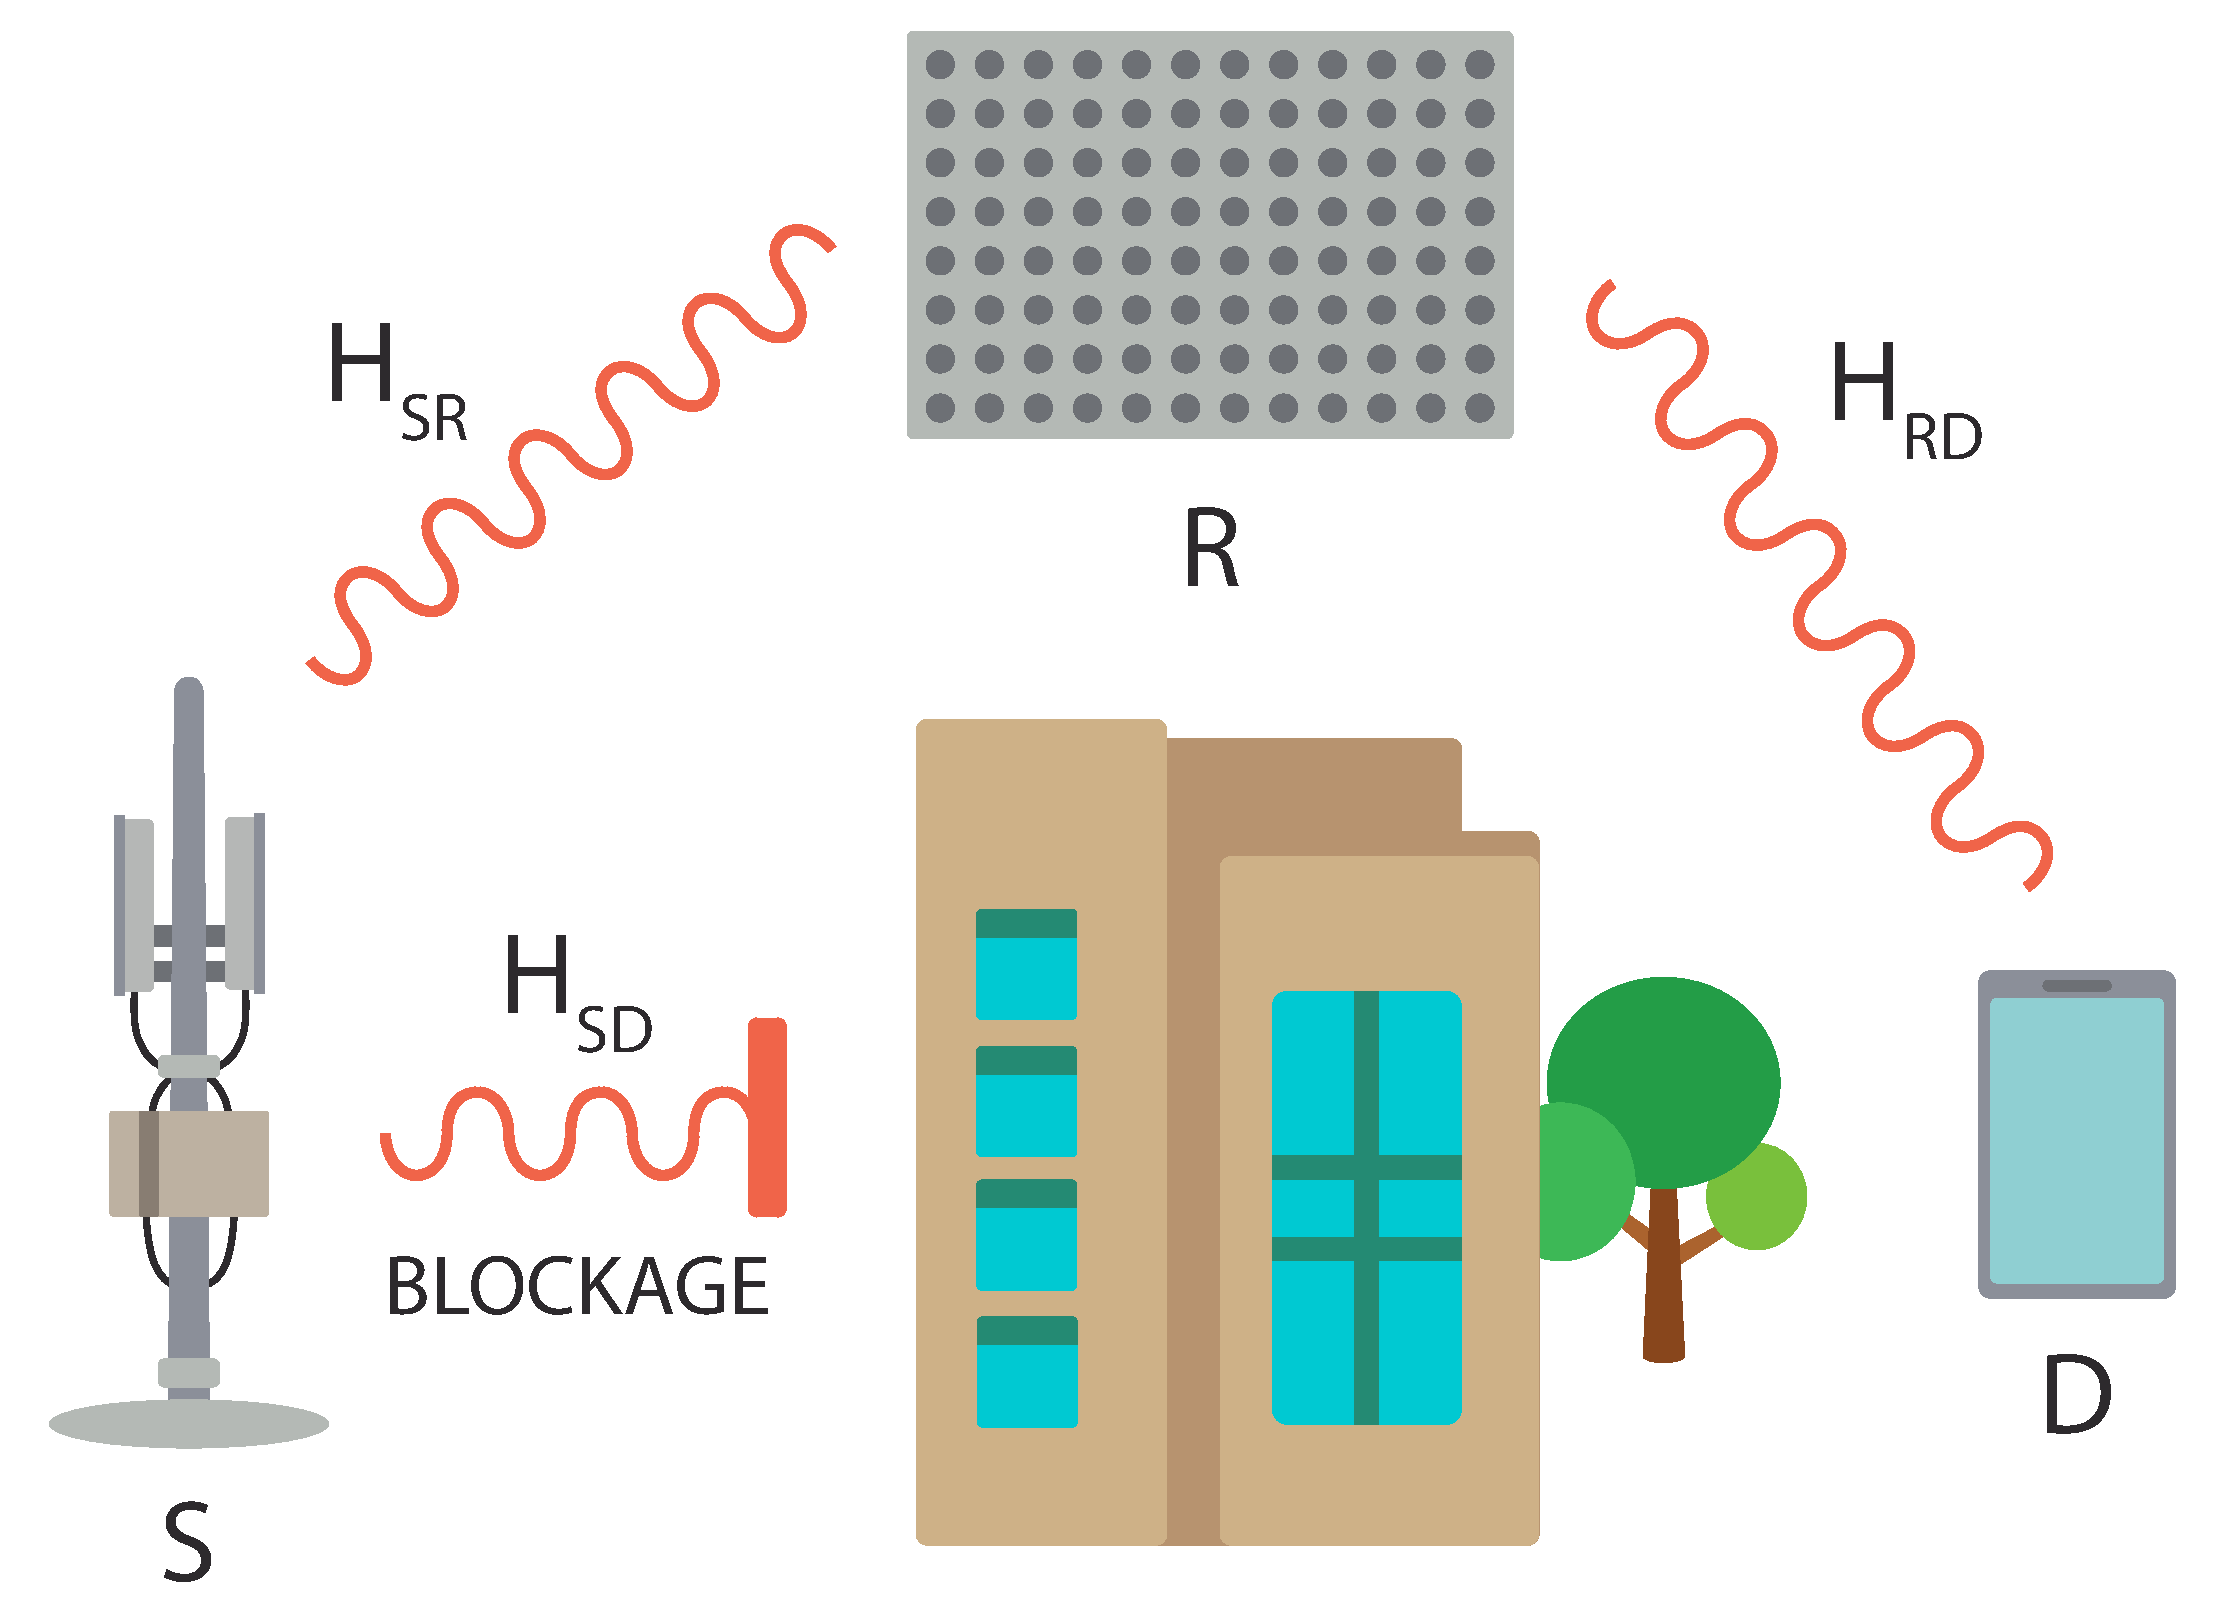
\includegraphics[width=0.75\textwidth]{Figures/IrsSimulation/Scenario_high_level.pdf}
  \caption{A typical urban scenario where a relay (R) can be used to bridge the signal from a source (S) to a destination (D), that would otherwise communicate in \acrshort{nlos}, i.e., the direct link between S and D is blocked due to obstacles such as buildings and/or vegetation.}
  \label{Fig:scenario_high_lvl}
\end{figure}

We consider the transmission of a single data stream $x_{\mathrm S}$, i.e., a sequence of signals, from a source S to a destination D via a relay R, as depicted in Figure~\ref{Fig:scenario_high_lvl}. 
Then, the channel matrix is combined with the beamforming vectors used at S and D, in order to obtain the \gls{sinr} experienced at D. 
In particular, let $x_{\mathrm S}$ be the signal transmitted from S to D, and $\bm{w}_{\mathrm S}$, $\bm{w}_{\mathrm D}$ and $\bm{w}_{\mathrm I}$ be the beamforming vectors used at S, D and the I-th interferer, respectively. Moreover, we define the following matrices:
$\bm{H}_{\mathrm SD}$ is the channel matrix between the source and the destination,
 $\bm{H}_{\mathrm ID}$ is the channel matrix between the \mbox{I-th} interferer and the destination,
 $\bm{H}_{\mathrm IR}$ is the channel matrix from the \mbox{I-th} interferer to the relay,
 $\bm{H}_{\mathrm SR}$ is the channel matrix between the source and the relay,
 and $\bm{H}_{\mathrm RD}$ is the channel matrix between the relay and the destination.
% $\bm{H}_{\mathrm SD}$ and $\bm{H}_{\mathrm ID}$ be the matrices of the S-D channel and the channel from the I-th interferer to D, respectively. 
In a relay-free environment, the signal received at the \gls{ue} is computed as:
\begin{equation}
    \label{eq:input_output_nodev}
    y_{\mathrm D} = \bm{w}_{\mathrm D}^{T} \bm{H}_{\mathrm SD} \bm{w}_{\mathrm S} x_{S} + \sum_{\mathrm{I}=1}^{N} \bm{w}_{\mathrm D}^{T} \bm{H}_{\mathrm ID}  \bm{w}_{\mathrm I} x_{\mathrm I} + \bm{w}_{\mathrm D}^{T} \bm{n}_{\mathrm D}.
\end{equation}
where $\bm{n}_D$ represents the circularly symmetric complex Gaussian noise vector with correlation matrix $\sigma_{\mathrm N}^2 \bm{I} $, and $\bm{w}_{\mathrm D}^{T} \bm{H}_{\mathrm ID} \bm{w}_{\mathrm I} x_{\mathrm I}$ is the signal received from the $\mathrm I$-th interferer.
Accordingly, the \gls{sinr} at D reads:
\begin{equation}
	\Lambda = \frac{ \lVert \bm{w}_{ \textrm D}^{T} \bm{H}_{\textrm {SD}}\bm{w}_{ \textrm S} \rVert^2 \sigma_{\mathrm S}^2 } { \sum_{\mathrm{I}=1}^{N} \lVert \bm{w}_{\mathrm D}^{T} \bm{H}_{\mathrm ID} \bm{w}_{\mathrm I} \rVert^2 \sigma_{\mathrm I}^2 + \sigma_{\mathrm N}^2 },
\end{equation}
where $\sigma_{\mathrm S}^2$ and $\sigma_{\mathrm I}^2$ are the powers of the intended and the $\mathrm{I}$-th interfering signals, respectively.
\subsection{A Signal Model for the IRS}
\label{sec:irs_phy_model} 
An \gls{irs} is a planar surface made of $N_{\mathrm R}$ low-cost passive reflecting elements that can be programmed to alter an \gls{em} field, for example to achieve three-dimensional beamforming towards an intended destination.
The working principle is similar to that of a conventional relay, the main difference being that while the latter amplifies the received signal before retransmitting it, an \gls{irs} reflects and beamforms the signal without introducing any amplification, thus saving power compared with other relaying solutions~\cite{bjornson2019intelligent}. %but promising lower gains as well. 


%However, in general the \gls{irs} is assumed to feature no signal processing capabilities.  

In particular, each element of the \gls{irs} acts as an 
%omnidirectional 
antenna that captures and reflects the incoming signals, introducing a phase shift on the baseband-equivalent signal. We denote with $\phi_n=e^{j\theta_n}, \, n = 1, \ldots, N_{\mathrm R}$, the reflection coefficient of the $n$-th \gls{irs} element, where $\theta_n \in [-\pi,\pi ] $ is the induced, controllable phase shift. 
Adopting a complex baseband notation, the signal $\bm{z} \in {\mathbb C}^{N_{\mathrm R} \times 1} $ reflected by an IRS (denoted as R), impinged with a signal $x_{\mathrm S}$ originating from a source S, reads
%When impinged with a signal $\bm{x}_{\mathrm S}$ originating from a source S, an \gls{irs} reflects the signal $\bm{z} \in {\mathbb C}^{N_{\mathrm R} \times 1} $, i.e.,
\begin{equation}
\bm{z}=\bm{\Phi}\bm{H}_{\mathrm SR} \bm{w}_{\mathrm S} x_{\mathrm S} ,
\end{equation}
%where $\bm{H}_{\mathrm SR}$ denotes the channel matrix between S and R, 
where $\bm{\Phi}$ is a diagonal matrix defined as $\bm{\Phi} \doteq \mathrm{diag} (\phi_1,\ldots,\phi_{N_{\mathrm R}})$, and typically referred to as {\em \gls{irs} configuration}. 
Therefore, the signal received at the intended destination D (under a far-field assumption with respect to the \gls{irs}) can be expressed as
\begin{equation}
	\label{eq:irs_iput_output}
    y_{\mathrm D} = \bm{w}_{\mathrm D}^{T} \bm{H}_{\mathrm RD} \bm{\Phi} \bm{H}_{\mathrm {SR}}  \bm{w}_{\mathrm S} x_S + \bm{w}_{\mathrm D}^{T} \bm{H}_{\mathrm SD} \bm{w}_{\mathrm S} x_S + \bm{w}_{\mathrm D}^{T} \bm{n}_{\mathrm D}.
\end{equation}
%where $\bm{H}_{\mathrm RD}$ denotes the matrix of the channel between the relay and the destination.
 
 \subsection{A Signal Model for the AF Relay}
 \label{sec:af_phy_model}
 
  \Gls{af} relays have been studied in the context of cooperative communications as a means to regenerate a relayed signal through amplification, with the goal of improving the system capacity. % And extending coverage?
  %The power amplifier entails that the gain of the AF relay is higher than that of a passive IRS when the number of IRS elements is equal to that of the AF relay antennas~\cite{huang2019reconfigurable}. On the downside, 
  Unlike \glspl{irs}, \gls{af} relays feature a non-negligible power consumption, and introduce noise amplification.

In this work we consider as \gls{af} relay a device equipped with $M_{\mathrm T}$ transmit and $M_{\mathrm R}$ receive antennas.
% two back-to-back panels of $M_{\mathrm R}$ antennas which first applies a receive beamforming vector $\bm{w}_{\mathrm R, RX}$ to obtain a single signal stream. Then, it amplifies and retransmits the latter using the transmit beamformer $\bm{w}_{\mathrm R, TX}$ and introducing an amplification $\mu_{\mathrm R}$. 
Therefore, the signal received at D is:
\begin{align}
\label{eq:af_iput_output}
    y_{\mathrm D} = \,\, &\bm{w}_{\mathrm D}^{T} \bm{H}_{\mathrm RD} \bm{\Phi} \bm{H}_{\mathrm {SR}} \bm{w}_{\mathrm S} x_{\mathrm S} + \bm{w}_{\mathrm D}^{T} \bm{H}_{\mathrm SD} \bm{w}_{\mathrm S} x_{\mathrm S}  \nonumber \\
   &+ \bm{w}_{\mathrm D}^{T} \bm{H}_{\mathrm RD} \bm{\Phi} \bm{n}_{\mathrm R} + \bm{w}_{\mathrm D}^{T} \bm{n}_{\mathrm D},
\end{align}
where in this case matrix $\bm{\Phi}$ also accounts for the amplification gain, and its structure depends on the specific relay design.
%\begin{equation}
%    \bm{\Phi} = \mu_{\mathrm R} \bm{w}_{\mathrm R, TX}  \bm{w}^T_{\mathrm R, RX}
%    \label{eq:phi_AF}
%\end{equation}
%is the rank-1 \gls{af} relay matrix obtained by multiplying the receive and transmit relay beamforming vectors $\bm{w}_{\mathrm R, RX}$ and $\bm{w}_{\mathrm R, TX}$, respectively. 
%Notice that, unlike for the \gls{irs}, matrix $\bm{\Phi}$ in~\eqref{eq:phi_AF} modeling the relay is not diagonal, since it is the result of the product of two beamforming vectors. 
Moreover, $\bm{n}_{\mathrm R}$ represents the circularly symmetric complex Gaussian noise vector with covariance matrix $\sigma_{\mathrm N_R}^2 \bm{I}_{M_{\mathrm R}} $.
Then, the power of the noise term relayed by the \gls{af} relay to receiver D and measured after the combiner at the \gls{ue}, is
\begin{equation} 
\label{eq:af_noise_power}
    \begin{split}
        \hat{\sigma}_{\mathrm N_R}^2 &= \left( \bm{w}_{\mathrm D}^{T} \bm{H}_{\mathrm RD} \bm{\Phi} \right) \left( \bm{w}_{\mathrm D}^{T} \bm{H}_{\mathrm RD} \bm{\Phi} \right)^{H} \sigma_{\mathrm N_R}^2 \\
         & = \bm{w}_{\mathrm D}^{T} \bm{H}_{\mathrm RD} \bm{\Phi} \bm{\Phi}^{H} \bm{H}_{\mathrm RD}^{H} {\bm w}^{*}_{\mathrm D} \sigma_{\mathrm N_R}^2.
    \end{split}
\end{equation}

%Furthermore, throughout this work we consider the \gls{af} relay to feature a \gls{pa} with a constraint on the maximum emitted power $P_{\mathrm max}$, due to saturation phenomena. 
%As such, $P_{\mathrm max}$ is a design parameter chosen a priori. 
%Moreover, we assume that the \gls{pa} has a maximum amplification factor $\mu_{\max}^2$.
%Under these assumptions, and using the above notation, the signal received at the %relay can be written as:
%\begin{equation}
%    y_{\mathrm R} = \bm{w}_{\mathrm R, RX}^{T} \bm{H}_{\mathrm {SR}} \bm{w}_{\mathrm S} x_{\mathrm S} + %\bm{w}_{\mathrm R, RX}^{T} \bm{n}_{\mathrm R}
%\end{equation}
%Then, assuming that the single-stream signal $x_{\mathrm S}$ has zero mean and variance $\sigma_{\mathrm S}^2$, the power of $y_{\mathrm R}$ can be expressed~as:
%\begin{equation}
%    P_{\mathrm R} = \left| \bm{w}_{\mathrm R, RX} ^{T} \bm{H}_{\mathrm {SR}} \bm{w}_{\mathrm S} \right|^2 \sigma_{\mathrm S}^2 + \sigma_{\mathrm N}^2.
%\end{equation}
%Thus, the amplification factor introduced by the relay is
%\begin{equation} \label{eq:af-amplif}
%    \begin{split}
%        \mu_{\mathrm R}^2 &= \min \left\{ \frac{P_{\mathrm max}}{ P_{\mathrm R}}, \, \mu_{\max}^2 \right\} \\
%        & = \min \left\{ \frac{P_{\mathrm max}}{\left| \bm{w}_{\mathrm R, RX}^{T} \bm{H}_{\mathrm {SR}} \bm{w}_{\mathrm S} \right|^2 \sigma_{\mathrm S}^2 + \sigma_{\mathrm N}^2}, \, \mu_{\max}^2 \right\}.
%    \end{split}
%\end{equation}

\subsection{A Full-Stack Simulator for IRS/AF Relays}
\label{sec:simulator}

Despite the availability of accurate sub-6 GHz and \gls{mmwave} channel models, analytical evaluations of the \gls{5g} NR protocol stack introduce several assumptions in the system architecture, and are generally not desirable~\cite{gkonis2020comprehensive}. 
%Moreover, \gls{5g} and beyond research is focusing on disruptive technologies, such as \glspl{irs}~\cite{8796365} and \glspl{ntn}~\cite{giordani2020non}, which are both extremely costly to test in the field, especially in their preliminary research phase.
Additionally, 5G/6G cellular networks are rapidly shifting towards open and controllable network configurations, which further introduce unprecedented data-driven programmability~\cite{bonati2020open}. 
In these regards, computer simulators are emerging as a valuable tool to let researchers better understand the performance of wireless networks, and dimension them accordingly~\cite{wilhelmi2021usage}.  

Several simulators for 5G cellular and vehicular networks are available in the literature~\cite{mezzavilla2018end,choi20195g, nardini2020simu5g, patriciello2019e2e, pratschner2018versatile, muller2018flexible, jao2018wise,drago2020millicar}. However, they provide a detailed characterization of either the lower (i.e., at the link level) or the upper (i.e., at the system level) layers of the \gls{5g} NR protocol stack. 
%Accordingly, they are typically referred to as link-level or system-level simulators, respectively. 
Notably, the latter sacrifice \gls{phy} layer accuracy to reduce the computational complexity, but incorporate accurate models of the remainder of the protocol stack, thus enabling scalable end-to-end simulations.
Despite the many software-based evaluation platforms available, to the best of our knowledge there are no end-to-end simulators for IRSs and AF relays. In~\cite{polese2018end}, the authors presented an open-source module for \gls{iab}, even though it was not extended to support passive relays like IRSs. 
Moreover, the authors in~\cite{heimann2021modeling} presented an ns-3 \gls{irs} module, but their work focused on vehicular networks, and did not consider the case of AF~relays. 

In this paper we close the gap and propose an ns-3-based simulator for IRSs and AF relays.
Arguably, the main effect of the presence of these entities is the alteration of the wireless channel between the communication endpoints. 
%This implies that the \gls{sinr} experienced over such channel will also be different compared to the case where no relays are deployed. 
Accordingly, our simulator extends the \texttt{ns-3 mmwave} module~\cite{mezzavilla2018end} (among the most popular 5G-oriented NR-compliant frameworks to simulate 5G networks) by implementing a new signal model for IRS and AF relays, following the characterization in Secs.~\ref{sec:irs_phy_model} and \ref{sec:af_phy_model}, respectively, which is then used to compute the \gls{sinr} experienced by signals transmitted over a relayed wireless link. 

%the bulk of our simulator consists in the implementation of a channel model for IRS and AF relays, based on the characterization in Secs.~\ref{sec:irs_phy_model} and \ref{sec:af_phy_model}, which is then used to compute the \gls{sinr} experienced by signals transmitted over a relayed wireless link. 
 


\subsubsection{Implementation of the IRS/AF Signal Model} 
\label{sec:ext_ch_model}
 
In line with~\cite{zugno2020implementation}, we assume that the transmission of the signal $x_{\mathrm S}$ occurs over a frequency-selective wireless channel as \gls{5g} NR supports network operations with a bandwidth up to 400 MHz, when using FR2~\cite{38101_1}. 
Therefore, the evaluation of the \gls{sinr} requires, among other things, the computation of the \gls{psd} of the useful component of the signal at D, i.e., $\mathcal{P}_{r x}$, starting from that of the input signal $\mathcal{P}_{t x}$. Additionally, we consider that both the transmitter and the receiver feature \gls{m-mimo} arrays equipped with multiple antenna elements, and use the beamforming vectors $\bm{w}_{\textrm S}$ and $\bm{w}_{\textrm D}$, respectively.
Under these assumptions, the input-output relationship in~\eqref{eq:input_output_nodev} becomes~\cite{bjornson2019intelligent, wu2019intelligent}:
\begin{equation}
\label{eq:mimo_input_output_relay}
\begin{aligned}
	y_{D} = \,\, & \bm{w}_{\mathrm D}^{\mathrm T} \bm{H}_{\mathrm RD} \bm{\Phi} \bm{H}_{\mathrm {SR}} \bm{w}_{\mathrm S} x_{S} + \bm{w}_{\mathrm D}^{T} \bm{H}_{\mathrm SD} \bm{w}_{\mathrm S} x_{S} + \tilde{n} + \\
	& \sum_{\mathrm{I}=1}^{N} \bm{w}_{\mathrm D}^{T} \bm{H}_{\mathrm {RD}} \bm{\Phi} \bm{H}_{\mathrm {IR}}  \bm{w}_{\mathrm I} x_{\mathrm I} + \sum_{\mathrm{I}=1}^{N} \bm{w}_{\mathrm D}^{T} \bm{H}_{\mathrm ID}  \bm{w}_{\mathrm I} x_{\mathrm I},
\end{aligned}
\end{equation}
where in turn $\tilde{n}$ is defined as:
\[ 
\tilde{n} = 
\begin{cases}
    \bm{w}_{\mathrm D}^{T} \bm{n}_{\mathrm D}		& \text{if IRS}, \\
    \bm{w}_{\mathrm D}^{T} \bm{n}_{\mathrm D} + \bm{w}_{\mathrm D}^{T} \bm{H}_{\mathrm RD} \bm{\Phi} \bm{n}_{\mathrm R}      & \text{if AF},
\end{cases}
\]
where matrix $\bm{\Phi}$ is the relay matrix, i.e., a matrix which fully encodes the effect of the relay, i.e., either IRS or AF, as described in Secs.~\ref{sec:irs_phy_model} and~\ref{sec:af_phy_model} for the single user case, respectively, over the wireless channel. 
%The terms $\bm{H}_{\mathrm {SR}}$, $\bm{H}_{\mathrm {IR}}$, $\bm{H}_{\mathrm {RD}}$ represent the channel matrices between the source and the relay, the $\mathrm{I}$-th interferer and the relay, and the relay and the destination, respectively. Moreover, $\bm{H}_{\mathrm {SD}}$, $\bm{H}_{\mathrm {ID}}$ are the channel matrices of the direct link from the source and the $\mathrm{I}$- th interferer to the destination, as illustrated in Figure~\ref{Fig:scenario_high_lvl}.
Notably, S and D are either in \gls{nlos} (in this case they communicate via the relay, and we consider the direct link towards D to be unavailable), or in \gls{los} (in this case they do not use the relay). % thus we consider the secondary path reflected by such entity to be negligible.
%These assumptions are motivated by the fact that we envision as the main use case for these kinds of relays scenarios in which the direct path between S and D is almost completely blocked by obstacles, such as building and/or vegetation.
Accordingly, assuming that the source of interest is in NLOS with respect to its intended destination,~\eqref{eq:mimo_input_output_relay} becomes:

\begin{equation}
\label{eq:mimo_input_output_relay_reduced}
\begin{aligned}
    y_{D} = \,\, & \bm{w}_{\mathrm{D}}^{\mathrm{T}} \bm{H}_{\mathrm{RD}} \bm{\Phi} \bm{H}_{\mathrm{SR}} \bm{w}_{\mathrm{S}} x_{S} + \sum_{\hat{I} \in  I_{\mathrm{LOS}}} \bm{w}_{\mathrm{D}}^{T} \bm{H}_{\mathrm{\hat{I}} D} \bm{w}_{\mathrm{\hat{I}}} x_{\mathrm{\hat{I}}} \\
  & + \sum_{ \bar{I} \in I_{\mathrm{NLOS}}} \bm{w}_{\mathrm{D}}^{T} \bm{H}_{\mathrm{RD}} \bm{\Phi} \bm{H}_{\mathrm{\bar{I} R}}  \bm{w}_{\mathrm{\bar{I}}} x_{\mathrm{\bar{I}}} + \tilde{n},
\end{aligned}
\end{equation}
where $I_{\mathrm{LOS}}$ and $I_{\mathrm{NLOS}}$ are the two disjoint sets of interferers which experience either an \gls{los} or an \gls{nlos} channel towards D, respectively.
Then, the \gls{psd} of the useful component of the signal at the receiver can be written as:
\begin{equation}
\label{eq:psd_relay}
\mathcal{P}_{r x}(t, f) = \mathcal{P}_{t x}(t, f) \lVert \bm{w}_{\textrm D}^{\textrm T} \bm{H}_{\textrm {RD}} \bm{\Phi} \bm{H}_{\textrm {SR}} \bm{w}_{\textrm S} \rVert^2.
\end{equation}

Based on the above definitions, our simulator computes the \gls{psd} by checking whether the communication from S to D involves a relay. 
If so, the \gls{psd} is computed according to the following steps.

\begin{enumerate}
    \item \emph{Channel matrices generation.} 
%First of all, we identify the relay's antennas communicating towards S and D. 
%For the sake of using a general model tailored to both forms of relays (i.e., IRS and AF), we assume that R features two antenna arrays, possibly pointing to different directions. %Depending on the type of relay, these arrays might then coincide in practice. 
After having identified S and D as the two endpoints of the communication, the channel matrices $\bm{H}_{\textrm {SR}}$ and $\bm{H}_{\textrm {RD}}$ are computed based on~\eqref{eq:ch_model_full_irs_sim}~\cite{3gpp.38.901}. 

\item \emph{Configuration of the relay and beamforming vectors.}
We assume that the choice of the beamforming vectors for both S and D ($\bm{w}_{\textrm D}$ and $\bm{w}_{\textrm S}$), as well as the relay configuration ($\bm{\Phi}$), consist in the choice of a \emph{codeword} from a pre-defined \emph{codebook}. The latter is computed offline by first defining a set of beam directions $\{ \omega_{n, m} \}$ which scan a given angular sector via steps of \gls{hpbw}. In particular, let $\bm{a}_{n,m}$ be the steering vector corresponding to direction $\omega_{n, m}$. This is computed~as:
\medmuskip=1mu
\thinmuskip=1mu
\thickmuskip=1mu
\begin{equation}
\begin{aligned}
    \bm{a}_{n, m} & =  \left[ 1,\ldots, e^{j\frac{2\pi}{\lambda}d\left(i_{\mathrm H}\sin\alpha_n\sin\beta_m+i_{\mathrm V}\cos\beta_m\right)}, \ldots, \right. \\ 
    & \left. e^{j\frac{2\pi}{\lambda}d\left((N_{\mathrm H}-1)\sin\alpha_n\sin\beta_m+(N_{\mathrm V}-1)\cos\beta_m\right)}\right]^T,
\end{aligned}
\end{equation}
\medmuskip=6mu
\thinmuskip=6mu
\thickmuskip=6mu
where $0 \leq i_{\mathrm H} \leq N_{\mathrm H}$ ($0 \leq i_{\mathrm V} \leq N_{\mathrm V}$) is the horizontal (vertical) index of an antenna element, $N_{\mathrm H}$ and $N_{\mathrm V}$ are the number of antenna elements in the horizontal and vertical direction, respectively, and $\alpha_n$ and $\beta_m$ represent the azimuth and the elevation angles of $\omega_{n, m}$, respectively. Then, we define the codeboook for the \glspl{ue}, \glspl{gnb} and \gls{af} relays as the set $\{ \left( \sqrt{N_{\mathrm H} N_{\mathrm V}} \right)^{-1} \bm{a}_{n, m} \}$, while the \gls{irs} codebook is defined as $\{ \bm{a}_{n, m} \}$. 
%Notably, for the \gls{irs} codebook the normalization term $ \left( \sqrt{N_{\mathrm H} N_{\mathrm V}} \right)^{-1}$ is not present, since the power of any impinging signal must be completely re-radiated by each \gls{irs} element.

Moreover, we assume that the devices do not have full channel knowledge, i.e., they do not know the realizations of $\bm{H}_{\textrm {SR}}$ and $\bm{H}_{\textrm {RD}}$. 
Then, in line with the \gls{5g} NR beam management procedure~\cite{giordani2018tutorial}, the choice of the codeword in the codebook is performed via exhaustive search, i.e., by repeatedly sending pilot signals, and measuring the \gls{sinr} experienced with various configurations of the codebook. Eventually, we choose the combination of $\bm{w}_{\textrm D}$, $\bm{w}_{\textrm S}$, and $\bm{\Phi}$ yielding the highest \gls{sinr}.

Notably, this procedure is not repeated at each transmission opportunity. Instead, $\bm{w}_{\textrm D}$, $\bm{w}_{\textrm S}$, and $\bm{\Phi}$ are stored and re-used for the whole channel coherence time, to mimic the actual 5G NR beam management procedure, and also reduce the complexity of the simulations. 
Furthermore, the evaluation of the \gls{sinr} is performed by neglecting the small-scale fading terms, to further reduce the overhead. The small-scale fading will be eventually incorporated in Step 4 of the model.

\item \emph{Long-term computation.} 
%The computation of the \gls{psd} at the receiver is decomposed into two sub-parts, . As such, 
%by explicitly outlining the vector and matrices products of Eq.~\ref{eq:psd_relay} 
Along the lines of~\cite{zugno2020implementation}, the \gls{psd} of the transmitted signal $x_S$ at D can be expressed as:
\begin{equation}
\begin{aligned}
&\mathcal{P}_{r x}(t, f) = \\
& = \mathcal{P}_{t x}(t, f) \lVert \bm{w}_{\textrm D}^{\textrm T} \bm{H}_{\textrm {RD}} \bm{\Phi} \bm{H}_{\textrm {SR}} \bm{w}_{\textrm S} \rVert^2 \\
&=\mathcal{P}_{t x}(t, f) \lVert \bm{w}_{\textrm D}^{\textrm T} \bm{H}_{\textrm {SRD}} \bm{w}_{\textrm S} \rVert^2 \\
& = \mathcal{P}_{t x}(t, f) \left\lVert \sum_{d=1}^{N_D} \sum_{s=1}^{N_S}  w^{\textrm D}_{d} h^{\mathrm SRD}_{d, s} (t, f)  w^{\textrm S}_{s} \right\rVert^2.
\end{aligned}
\label{eq:p-rx-sdr}
\end{equation}

In Eq.~\eqref{eq:p-rx-sdr}, $\bm{H}_{\mathrm SRD}$ is the equivalent channel matrix between S and D, whose generic entry  $h^{\mathrm SRD}_{d, s} (t, f)$ is:
\begin{equation}
\begin{aligned}
\label{eq:psd_relay_sums}
h^{\mathrm SRD}_{d, s} (t, f) &= \left[ \bm{H}_{\textrm {RD}} (t, f) \bm{\Phi} \bm{H}_{\textrm {SR}} (t, f) \right]_{d, s} \\
& = \sum_{n=1}^{N_{\mathrm RD}} \sum_{m=1}^{N_{\mathrm SR}} \sum_{k=1}^{N_{R}} \sum_{l=1}^{N_{\mathrm R}} h^{\mathrm RD}_{d, k, n} \, \phi_{k, l} \, h^{\mathrm SR}_{l, s, m} \\
& \quad \times e^{j 2 \pi v_{n} t} e^{j 2 \pi \tau_{n} f} \\
& \quad \times e^{j 2 \pi v_{m} t} e^{j 2 \pi \tau_{m} f},
\end{aligned}
\end{equation}
where $N_{\mathrm RD}$ and $N_{\mathrm SR}$ are the number of multipath clusters in $\bm{H}_{\textrm {RD}}$ and $\bm{H}_{\textrm {SR}}$, respectively. Moreover, $w^{\textrm S}_{s}$ and $w^{\textrm D}_{d}$ denote entries $s$ and $d$ of vectors $\bm{w}_{\mathrm S}$ and $\bm{w}_{\mathrm D}$, respectively.
Then, Step 3 consists in the evaluation of the long-term fading:
\begin{equation}
L_{n, m} \doteq \sum_{d=1}^{N_{\mathrm D}} \sum_{s=1}^{N_{\mathrm S}} \sum_{k=1}^{N_{\mathrm R}} \sum_{l=1}^{N_{\mathrm R}} w^{\mathrm D}_{d} \, h^{\mathrm RD}_{d, k, n} \, \phi_{k, l} \, h^{\mathrm SR}_{l, s, m} \, w^{\mathrm S}_{s}. 
\end{equation}
%which involves the terms in the summations of Eq.~\eqref{eq:psd_relay_sums} which vary relatively slowly over time only.

\item \emph{Small-scale fading and path loss.}
The small-scale fading terms are combined with the terms $L_{n, m}$ to compute the overall fading component of the \gls{psd} of interest:
\begin{equation}
	\mathcal{\tilde{P}}_{rx}(t, f) = \mathcal{P}_{t x}(t, f) \left\lVert \sum_{n=1}^{N_{\mathrm RD}} \sum_{m=1}^{N_{\mathrm SR}} L_{n, m} E_{n, m}  \right\rVert^2,
\end{equation}
% A bit tedious to read, but could not fit in a single line otherwise..
where
\begin{equation}
E_{n, m} \doteq e^{j 2 \pi v_{n} t} e^{j 2 \pi \tau_{n} f} e^{j 2 \pi v_{m} t} e^{j 2 \pi \tau_{m} f}.
\end{equation}
Additionally, the path loss is computed as in~\eqref{eq:pl}. Since the useful signal received at D experiences two channels (from S to R, and from R to D) as a cascade, as described in~\eqref{eq:mimo_input_output_relay}, two path loss terms are added (in dB), to obtain the final \gls{psd} of $x_S$ at D as:
\begin{equation}
\begin{split}
\mathcal{P}_{r x}(t, f)& [\mathrm{dB}]  = \text{PL} (d_{\mathrm{SR}}, f_c) [\mathrm{dB}] \\
& + \text{PL} (d_{\mathrm{RD}}, f_c) [\mathrm{dB}] + \mathcal{\tilde{P}}_{rx}(t, f) [\mathrm{dB}].
\end{split}
\end{equation}
\item \emph{Interference and \gls{sinr}.}
As the last step, we evaluate the \glspl{psd} $\{ \mathcal{P}_{i}(t, f) \}_{i = 1, \dots, N_I}$ of the $N_I$ interfering signals at D. %The same assumptions are introduced, i.e., for \gls{los} (\gls{nlos}) devices the relayed (direct) link is neglected. 
To do so, we follow Steps 1--4 as for the useful component of the signal. However, the beamforming configurations are not optimized as described in Step 2. That is to say, each interferer uses the beamforming vector yielding the highest \gls{sinr} \emph{towards its intended destination}, while R and D employ the same configurations used in the previous steps.
Finally, the \gls{sinr} is evaluated as:
\[ \Lambda (t, f) = \frac{ \mathcal{P}_{r x}(t, f)} {\sum_{i=1}^{N_I} \mathcal{P}_{i}(t, f) + \mathcal{P}_{n}(t, f) },  \]
where $\mathcal{P}_{n}(t, f)$ is the \gls{psd} of the thermal noise at D.
\end{enumerate}

\subsubsection{Integration of the IRS/AF Signal Model in the Simulator}
In Section~\ref{sec:ext_ch_model} we described how our simulator computes the channel (in terms of \gls{psd}) in case of IRS/AF relays, which is then used to calculate the end-to-end SINR at the destination D. 
Notice that the \gls{sinr} can refer to either the \gls{sinr} relative to the whole bandwidth, for narrowband signals over frequency-flat channels, or the \gls{sinr} experienced over a single subcarrier, for wideband signals transmitted over frequency-selective channels. 
In the second case, the \glspl{sinr} corresponding to the various frequency chunks are then mapped into a single \gls{sinr} value, according to additional maps obtained from link-level simulations~\cite{lagen2020new}.
Based on that, our simulator defines a \gls{l2sm}, i.e., a table which associates a given \gls{sinr} to a \gls{mac}-layer \gls{tb} error rate~\cite{mezzavilla2012lightweight}, in turn used to  decide whether the \gls{tb} has been correctly received or not.
%At each transmission opportunity, the \gls{sinr} is computed, by simulating the wireless channel and possibly combining it with transmit and receive beamforming vectors.
%Finally, the \gls{l2sm} is used to map such \gls{sinr} to the error probability of the corresponding \gls{mac} \gls{tb} and, .

The upper layers of the 5G NR protocol stack are modeled based on the \texttt{ns3-mmwave} module~\cite{mezzavilla2018end}, which implements a custom \gls{phy} layer supporting the NR frame structures and numerologies, and a \gls{mac} layer with ad hoc beamforming and scheduling policies. 
The \gls{rlc} and \gls{pdcp} layers implement network functions such as packet segmentation, retransmissions and/or reassembly. 
%The module also supports non-standalone deployments, handover and mobility management via dual connectivity, and Carrier Aggregation (CA) at the MAC layer. 
%Based on these features, \texttt{ns3-mmwave} stands out as among the most popular 5G-oriented NR-compliant frameworks to simulate 5G networks.


%Since system-level simulators usually accurately model the \gls{mac} and above layers, in general they do not introduce any further abstraction. Therefore, they model all the complex protocols which are involved the NR protocol stack, from the \gls{mac} up to the \gls{sdap} or \gls{rrc} layers. 




%Among the various \gls{5g} simulators in the literature, link-level ones feature the most detailed modeling of the NRgls{nr} \gls{phy} layer. As such, they simulate each \gls{ofdm} sample, taking into account channel coding and decoding, estimation and equalization and, possibly, \gls{mimo} processing~\cite{pratschner2018versatile}. However, this accuracy comes at the price of a remarkable computational complexity, which usually limits the scope of these simulators to point-to-point transmissions only.
%Conversely, most \gls{ofdm} system-level simulators pre-process most of these computations and abstract most of the signal processing procedures, thus achieving much greater computational efficiency.


\subsection{Performance Evaluation}
\label{sec:results}

In this section we describe our simulation setup and parameters (Section~\ref{sub:simulation_setup}), and evaluate the performance of \glspl{irs} and \gls{af} relays, considering full-stack network metrics as a function of different antenna array configurations (Section~\ref{sub:numerical_results}).

\subsubsection{Simulation Setup} % (fold)
\label{sub:simulation_setup}

In our simulations we consider two simple yet realistic urban canyon scenarios, where we deploy a single \gls{gnb}, $N_{\mathrm U}$ \glspl{ue}, with $N_{\mathrm U}=1$ (5) in Scenario 1 (2), as illustrated in Figure~\ref{Fig:scenarios}, and a single relay, which can be either an \gls{irs} or an \gls{af} relay.
The wireless channel is modeled as an \gls{uma} link~\cite{3gpp.38.901}. % with the extensions discussed in Section~\ref{sec:ext_ch_model} to incorporate IRS/AF functionalities.
The \gls{los}/\gls{nlos} condition depends on the geometry of the scenario.
In particular, we assume that the direct wireless link between the \glspl{ue} and the \gls{gnb} is blocked by a building, as illustrated in Figure~\ref{Fig:scenarios}, which introduces an additional penetration loss modeled based on~\cite[Section 7.4.3.1]{3gpp.38.901}.
The end nodes can still communicate in \gls{los} via the relay. 
Furthermore, we assume that at each \gls{tti} the relays can arbitrarily switch configuration to serve a given user and that their phase shifters have infinite resolution, i.e., we do not account for quantization loss.
 
%The wireless channel is modeled as a TR. 38.901 \gls{uma} link, with the extensions discussed in Section~\ref{sec:ext_ch_model}. However, the \gls{los} condition is not stochastic as in~\cite[Section 7.4.2]{3gpp.38.901}. Instead, it is determined in a deterministic manner, based on the geometry of the scene.
%$Therefore, all $N_{\mathrm U}$ \glspl{ue} experience a \gls{nlos} link towards the \gls{gnb}, while the relay offers a two-hop \gls{los} path from the base station to the user terminals. Moreover, for the \gls{nlos} links we consider an additional loss term, computed as per~\cite[Section 7.4.3.1]{3gpp.38.901}.


%A building is placed in between the , in such a way to block the direct wireless link among them. On the contrary, we deploy the relay in an unobstructed location between the \gls{gnb} and the \glspl{ue}, as depicted in Figure~\ref{Fig:scenarios}.

Our simulation parameters are reported in Table~\ref{Tab:parameters}.
Specifically, the \glspl{ue} download \gls{udp} data, modeled as a constant bit-rate stream of 50~Mbps, from a remote server. 
We assume that, at each transmission opportunity towards the generic $k$-th \gls{ue}, both \gls{af} and \gls{irs} relays can use their optimal configuration, i.e., the codeword yielding the highest end-to-end \gls{sinr} towards \gls{ue} $k$.
The system operates at 28 GHz, with a total bandwidth of 100~MHz, to be shared among all the devices in \gls{tdma}. 
The gNB is equipped with an antenna array of 64 elements, and uses a power of 33 dBm.
For the IRS, we consider a number of reflecting elements from 200 to 7\,200.
For the AF relay, we consider antenna arrays from 16 to 256 elements.%, with a maximum amplifier output power of 25~dBm.

%In the remainder of this section we compare different relay configurations, featuring various antenna array configurations, to a baseline where no relay is present.

\begin{figure}[t!]
  \centering
    \begin{subfigure}[t]{\columnwidth}
    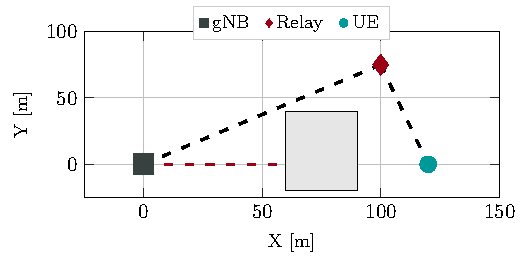
\includegraphics[width=0.75\columnwidth]{Figures/IrsSimulation/Scenario1.pdf}
    \caption{Scenario 1, with $N_{\mathrm U} = 1$.}
    \label{Fig:s1}
    \end{subfigure}
     \begin{subfigure}[t]{\columnwidth}
    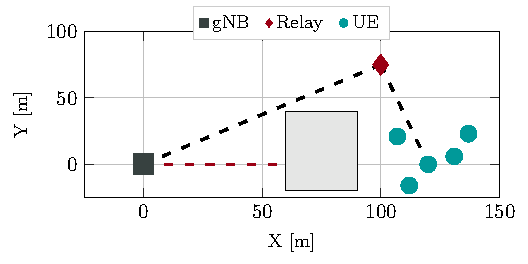
\includegraphics[width=0.75\columnwidth]{Figures/IrsSimulation/Scenario2.pdf}
    \caption{Scenario 2, with $N_{\mathrm U} = 5$.}
    \label{Fig:s2}
    \end{subfigure}
     \caption{Simulation scenarios, where we deploy one \gls{gnb}, $N_{\mathrm U}$ \glspl{ue} and, possibly, a relay. A building (the gray rectangle) blocks the direct link (dashed red line) from the \gls{gnb} to the \glspl{ue}. In turn, the relay guarantees a \gls{los} link (dashed black line) to all the devices.}
    \label{Fig:scenarios}
\end{figure}

%\setlength{\tabcolsep}{0.5em}
\def\arraystretch{1.3}
\begin{table}[t!]
  \caption{Simulation parameters.}
  \label{Tab:parameters}
  \centering
  \footnotesize
  \begin{tabular}{l|l}
    \toprule
    Parameter                  & Value \\ \midrule
    Carrier frequency		   & 28~GHz	\\
    Total bandwidth			   & 100~MHz \\
    Number of \glspl{ue} ($N_{\mathrm U}$)  & \{1, 5\} \\
    \gls{gnb} antenna array    & $8$H$\times8$V \\
    \gls{gnb} max RF power	   & 33~dBm \\
    \gls{ue} antenna array     & $2$H$\times1$V \\
    \gls{irs} antenna array    & \{$10$H$\times20$V, $20$H$\times40$V,$ 40$H$\times80$V, $60$H$\times120$V\} \\
    \gls{af} antenna array     & \{$4$H $\times4$V, $8$H $\times8$V, $16$H $\times16$V\} \\
    %\gls{af} max RF power	   & 25~dBm \\
    \gls{af} amplification & 40~dB \\
    Antenna radiation pattern  & \cite[Table 7.3-1]{3gpp.38.901} \\
    UDP source rate			   & 50~Mbps\\
    \bottomrule
  \end{tabular}
\end{table}




\subsection{Numerical Results} % (fold)
\label{sub:numerical_results}

We now compare the end-to-end performance of \gls{irs}- and \gls{af}-relay assisted networks in terms of:
\begin{itemize}
    \item \emph{\gls{sinr}}. It is a measure of the quality of the channel. 
    It depends on PHY-layer characteristics, including the relative distance between the transmitter, the receiver and the relay (if applicable), the operating frequency, the propagation conditions, %(for example whether the transmitter and the receiver are in \gls{los}) 
    and the channel bandwidth. %(which in turn affects the noise power
    \item \emph{End-to-end throughput}. %It is a measure of how fast we can send data through the network, and
     It is measured as the total number of received bytes per user divided by the total simulation time. 
%     Thanks to our accurate system-level simulator, we %refers to the overall effective transmission rate, 
 %   take into account issues like transmission overhead, protocol header and/or inefficiencies, and competing traffic. %It is therefore influenced by 
    %Moreover, both the type of application that is considered, as well as the underlying protocol stack, have an impact on this metric. 
    \item \emph{End-to-end latency.} It is measured from the time each packet is generated at the application layer to when it is successfully received.
  Accordingly, it accounts for both transmission and queuing times. %(which depends on the application, i.e., how fast packets are generated). 
 \item \emph{\gls{per}}. It is measured as the ratio between the number of packets delivered with errors and the total number of transmitted packets.
\end{itemize}
The IRS/AF performance will be evaluated against a baseline scenario (referred to as “gNB-only”) in which there is no intermediate relay.

\begin{figure}
  \centering
  \begin{subfigure}[t]{\columnwidth}
    \centering
    \setlength\fwidth{0.65\columnwidth}
    \setlength\fheight{0.28\columnwidth}
    % This file was created with tikzplotlib v0.9.12.
\begin{tikzpicture}

  \pgfplotsset{every tick label/.append style={font=\footnotesize}}
  \definecolor{plotColor1}{HTML}{E36B02}
  \definecolor{plotColor2}{HTML}{78BF26}
  \definecolor{plotColor3}{HTML}{572096}
  \definecolor{plotColor4}{HTML}{338EDE}
  \definecolor{plotColor1Light}{HTML}{F3C399}
  \definecolor{plotColor2Light}{HTML}{AABF95}
  \definecolor{plotColor3Light}{HTML}{827896}
  \definecolor{plotColor4Light}{HTML}{B2C8DE}
  \definecolor{color6}{rgb}{0.890196078431372,0.466666666666667,0.76078431372549}

\begin{axis}[
  width=\fwidth,
  height=\fheight,
  at={(0\fwidth,0\fheight)},
  scale only axis,
  legend image post style={mark indices={}},
  %axis line style={white!80!black},
  legend style={
      /tikz/every even column/.append style={column sep=0.2cm},
      at={(0.5, 1.03)}, 
      anchor=south, 
      draw=white!80!black, 
      font=\scriptsize
      },
  legend columns=4,
  %tick align=outside,
  %x grid style={white!80!black},
  xlabel style={font=\footnotesize},
  xtick align=inside,
  ytick align=inside,
  xlabel={SNR [dB]},
  %xtick={0,1,2,3,4,5,6,7},
  xmajorticks=true,
  xmajorgrids,
  %xmajorticks=false,
  xmin=-66, xmax=45,
  xtick style={color=white!15!black},
  %y grid style={white!80!black},
  ylabel shift = -1 pt,
  ylabel style={font=\footnotesize, align=center},
  ylabel={ECDF},
  ymajorgrids,
  %ymajorticks=false,
  ymin=0, ymax=1,
  ytick style={color=white!15!black},
]
\addplot [very thick, plotColor2]
table {%
-34.4357986450195 0
-34.4357986450195 0.00995051860809326
-33.9701995849609 0.0106005668640137
-33.9701995849609 0.0199509859085083
-30.8896999359131 0.0206010341644287
-30.8896999359131 0.0299514532089233
-30.7057991027832 0.0306015014648438
-30.7057991027832 0.0399520397186279
-30.3274993896484 0.0406019687652588
-30.3274993896484 0.049952507019043
-29.7175006866455 0.0506025552749634
-29.7175006866455 0.059952974319458
-28.6723003387451 0.0606030225753784
-28.6723003387451 0.069953441619873
-28.1532001495361 0.0706034898757935
-28.1532001495361 0.0799540281295776
-27.7136001586914 0.080604076385498
-27.7136001586914 0.0899544954299927
-27.183500289917 0.0906045436859131
-27.183500289917 0.0999549627304077
-27.1487007141113 0.100605010986328
-27.1487007141113 0.109955549240112
-26.2733993530273 0.110605478286743
-26.2733993530273 0.119956016540527
-25.9375 0.120606064796448
-25.9375 0.129956483840942
-25.8474998474121 0.130606532096863
-25.8474998474121 0.139956951141357
-25.5358009338379 0.140606999397278
-25.5358009338379 0.149957537651062
-25.167200088501 0.150607585906982
-25.167200088501 0.159958004951477
-25.1152000427246 0.160608053207397
-25.1152000427246 0.169958472251892
-25.1117000579834 0.170608520507812
-25.1117000579834 0.179959058761597
-23.8999996185303 0.180608987808228
-23.8999996185303 0.189959526062012
-23.6777000427246 0.190609574317932
-23.6777000427246 0.199959993362427
-23.2880992889404 0.200610041618347
-23.2880992889404 0.209960460662842
-22.9477996826172 0.210610508918762
-22.9477996826172 0.219961047172546
-22.7707004547119 0.220611095428467
-22.7707004547119 0.229961514472961
-22.5224990844727 0.230611562728882
-22.5224990844727 0.239961981773376
-22.2411994934082 0.240612030029297
-22.2411994934082 0.249962449073792
-21.1553001403809 0.250612497329712
-21.1553001403809 0.269963502883911
-20.9053001403809 0.270613551139832
-20.9053001403809 0.279963970184326
-20.7558002471924 0.280614018440247
-20.7558002471924 0.289964437484741
-20.2984008789062 0.290614604949951
-20.2984008789062 0.299965023994446
-20.2346992492676 0.300615072250366
-20.2346992492676 0.309965491294861
-19.9316997528076 0.310615539550781
-19.9316997528076 0.319965958595276
-19.7136001586914 0.320616006851196
-19.7136001586914 0.32996654510498
-19.6145000457764 0.330616474151611
-19.6145000457764 0.339967012405396
-19.4584999084473 0.340617060661316
-19.4584999084473 0.349967479705811
-19.1814994812012 0.350617527961731
-19.1814994812012 0.359967947006226
-19.1348991394043 0.360617995262146
-19.1348991394043 0.36996853351593
-19.0347003936768 0.370618581771851
-19.0347003936768 0.379969000816345
-18.9498996734619 0.380619049072266
-18.9498996734619 0.38996946811676
-18.94700050354 0.390619516372681
-18.94700050354 0.399970054626465
-18.8661003112793 0.400619983673096
-18.8661003112793 0.40997052192688
-18.6518001556396 0.4106205701828
-18.6518001556396 0.419970989227295
-18.6280002593994 0.420621037483215
-18.6280002593994 0.42997145652771
-18.5496997833252 0.43062150478363
-18.5496997833252 0.439972043037415
-18.4636993408203 0.440622091293335
-18.4636993408203 0.44997251033783
-18.2588005065918 0.45062255859375
-18.2588005065918 0.459972977638245
-18.135799407959 0.460623025894165
-18.135799407959 0.469973564147949
-17.9792995452881 0.47062349319458
-17.9792995452881 0.479974031448364
-17.9692001342773 0.480623960494995
-17.9692001342773 0.489974498748779
-17.9594993591309 0.4906245470047
-17.9594993591309 0.499974966049194
-17.8903007507324 0.500625014305115
-17.8903007507324 0.509975433349609
-17.738000869751 0.510625600814819
-17.738000869751 0.519976019859314
-17.3022003173828 0.520626068115234
-17.3022003173828 0.529976487159729
-17.2541007995605 0.530626535415649
-17.2541007995605 0.539977073669434
-16.8572998046875 0.540627002716064
-16.8572998046875 0.549977540969849
-16.8159008026123 0.550627470016479
-16.8159008026123 0.559978008270264
-16.5599002838135 0.560628056526184
-16.5599002838135 0.569978475570679
-16.3742008209229 0.570628523826599
-16.3742008209229 0.579978942871094
-16.0534992218018 0.580629110336304
-16.0534992218018 0.589979410171509
-16.0177001953125 0.590629577636719
-16.0177001953125 0.599979996681213
-15.847900390625 0.600630044937134
-15.847900390625 0.609980583190918
-15.5930995941162 0.610630512237549
-15.5930995941162 0.619981050491333
-15.2135000228882 0.620630979537964
-15.2135000228882 0.639981985092163
-15.1687002182007 0.640632033348083
-15.1687002182007 0.649982452392578
-15.1248998641968 0.650632619857788
-15.1248998641968 0.659982919692993
-14.9694995880127 0.660633087158203
-14.9694995880127 0.669983506202698
-14.9028997421265 0.670633554458618
-14.9028997421265 0.679983973503113
-14.8857002258301 0.680634021759033
-14.8857002258301 0.689984560012817
-14.6779003143311 0.690634489059448
-14.6779003143311 0.699985027313232
-14.3793001174927 0.700634956359863
-14.3793001174927 0.709985494613647
-14.3182001113892 0.710635542869568
-14.3182001113892 0.719985961914062
-14.0420999526978 0.720636010169983
-14.0420999526978 0.729986429214478
-13.9685001373291 0.730636596679688
-13.9685001373291 0.739987015724182
-13.8100004196167 0.740637063980103
-13.8100004196167 0.749987483024597
-13.644700050354 0.750637531280518
-13.644700050354 0.759988069534302
-13.3866996765137 0.760637998580933
-13.3866996765137 0.769988536834717
-13.2315998077393 0.770638465881348
-13.2315998077393 0.779989004135132
-12.9638004302979 0.780639052391052
-12.9638004302979 0.789989471435547
-12.8590002059937 0.790639519691467
-12.8590002059937 0.799989938735962
-12.1894998550415 0.800640106201172
-12.1894998550415 0.809990525245667
-12.0080003738403 0.810640573501587
-12.0080003738403 0.819990992546082
-11.5909996032715 0.820641040802002
-11.5909996032715 0.829991579055786
-11.5080003738403 0.830641508102417
-11.5080003738403 0.839992046356201
-11.3587999343872 0.840641975402832
-11.3587999343872 0.849992513656616
-10.9357995986938 0.850642561912537
-10.9357995986938 0.859992980957031
-10.5752000808716 0.860643029212952
-10.5752000808716 0.869993448257446
-10.2545003890991 0.870643615722656
-10.2545003890991 0.879993915557861
-8.57287979125977 0.880644083023071
-8.57287979125977 0.889994502067566
-8.56208038330078 0.890644550323486
-8.56208038330078 0.899995088577271
-8.37135982513428 0.900645017623901
-8.37135982513428 0.909995555877686
-7.63006019592285 0.910645484924316
-7.63006019592285 0.919996023178101
-7.58985996246338 0.920645952224731
-7.58985996246338 0.929996490478516
-5.78646993637085 0.930646538734436
-5.78646993637085 0.939996957778931
-5.43994998931885 0.940647006034851
-5.43994998931885 0.949997425079346
-4.19962978363037 0.950647592544556
-4.19962978363037 0.95999801158905
-2.7035698890686 0.960648059844971
-2.7035698890686 0.969998478889465
-1.87389004230499 0.970648527145386
-1.87389004230499 0.97999906539917
-1.38098001480103 0.980648994445801
-1.38098001480103 0.989999532699585
2.59274005889893 0.990649461746216
2.59274005889893 1
};
\addlegendentry{IRS 10x20}

\addplot [very thick, plotColor2, dashed]
table {%
-21.172399520874 0
-21.172399520874 0.00995051860809326
-20.6772994995117 0.0106005668640137
-20.6772994995117 0.0199509859085083
-19.2015991210938 0.0206010341644287
-19.2015991210938 0.0299514532089233
-18.9838008880615 0.0306015014648438
-18.9838008880615 0.0399520397186279
-18.1450004577637 0.0406019687652588
-18.1450004577637 0.049952507019043
-17.5377998352051 0.0506025552749634
-17.5377998352051 0.059952974319458
-17.105899810791 0.0606030225753784
-17.105899810791 0.069953441619873
-15.9405002593994 0.0706034898757935
-15.9405002593994 0.0799540281295776
-15.9084997177124 0.080604076385498
-15.9084997177124 0.0899544954299927
-15.0838003158569 0.0906045436859131
-15.0838003158569 0.0999549627304077
-15.0734996795654 0.100605010986328
-15.0734996795654 0.109955549240112
-14.9524002075195 0.110605478286743
-14.9524002075195 0.119956016540527
-14.923999786377 0.120606064796448
-14.923999786377 0.129956483840942
-14.1075000762939 0.130606532096863
-14.1075000762939 0.139956951141357
-13.8653001785278 0.140606999397278
-13.8653001785278 0.149957537651062
-13.7305002212524 0.150607585906982
-13.7305002212524 0.159958004951477
-13.4989004135132 0.160608053207397
-13.4989004135132 0.169958472251892
-13.2620000839233 0.170608520507812
-13.2620000839233 0.179959058761597
-12.8626003265381 0.180608987808228
-12.8626003265381 0.189959526062012
-12.4366998672485 0.190609574317932
-12.4366998672485 0.199959993362427
-12.3346996307373 0.200610041618347
-12.3346996307373 0.209960460662842
-10.6895999908447 0.210610508918762
-10.6895999908447 0.219961047172546
-10.3915996551514 0.220611095428467
-10.3915996551514 0.229961514472961
-10.3030004501343 0.230611562728882
-10.3030004501343 0.239961981773376
-10.1599998474121 0.240612030029297
-10.1599998474121 0.249962449073792
-9.8557596206665 0.250612497329712
-9.8557596206665 0.259963035583496
-9.66279983520508 0.260612964630127
-9.66279983520508 0.269963502883911
-9.55974006652832 0.270613551139832
-9.55974006652832 0.279963970184326
-9.45223045349121 0.280614018440247
-9.45223045349121 0.289964437484741
-8.82935047149658 0.290614604949951
-8.82935047149658 0.299965023994446
-8.80762004852295 0.300615072250366
-8.80762004852295 0.309965491294861
-8.78038024902344 0.310615539550781
-8.78038024902344 0.319965958595276
-8.64400959014893 0.320616006851196
-8.64400959014893 0.32996654510498
-8.48060989379883 0.330616474151611
-8.48060989379883 0.339967012405396
-8.40355968475342 0.340617060661316
-8.40355968475342 0.349967479705811
-8.23311042785645 0.350617527961731
-8.23311042785645 0.359967947006226
-7.94781017303467 0.360617995262146
-7.94781017303467 0.36996853351593
-7.9422402381897 0.370618581771851
-7.9422402381897 0.379969000816345
-7.7628698348999 0.380619049072266
-7.7628698348999 0.38996946811676
-7.73378992080688 0.390619516372681
-7.73378992080688 0.399970054626465
-7.65725994110107 0.400619983673096
-7.65725994110107 0.40997052192688
-7.43105983734131 0.4106205701828
-7.43105983734131 0.419970989227295
-7.33023023605347 0.420621037483215
-7.33023023605347 0.42997145652771
-7.1835298538208 0.43062150478363
-7.1835298538208 0.439972043037415
-7.13921022415161 0.440622091293335
-7.13921022415161 0.44997251033783
-6.57077980041504 0.45062255859375
-6.57077980041504 0.459972977638245
-6.38861989974976 0.460623025894165
-6.38861989974976 0.469973564147949
-6.08899021148682 0.47062349319458
-6.08899021148682 0.479974031448364
-6.03529977798462 0.480623960494995
-6.03529977798462 0.489974498748779
-6.00831985473633 0.4906245470047
-6.00831985473633 0.499974966049194
-5.48658990859985 0.500625014305115
-5.48658990859985 0.509975433349609
-5.47596979141235 0.510625600814819
-5.47596979141235 0.519976019859314
-5.45127010345459 0.520626068115234
-5.45127010345459 0.529976487159729
-5.24755001068115 0.530626535415649
-5.24755001068115 0.539977073669434
-5.15467977523804 0.540627002716064
-5.15467977523804 0.549977540969849
-5.10434007644653 0.550627470016479
-5.10434007644653 0.559978008270264
-5.01936006546021 0.560628056526184
-5.01936006546021 0.569978475570679
-4.77634000778198 0.570628523826599
-4.77634000778198 0.579978942871094
-4.54007005691528 0.580629110336304
-4.54007005691528 0.589979410171509
-4.38954019546509 0.590629577636719
-4.38954019546509 0.599979996681213
-4.37177991867065 0.600630044937134
-4.37177991867065 0.609980583190918
-4.16562986373901 0.610630512237549
-4.16562986373901 0.619981050491333
-3.83145999908447 0.620630979537964
-3.83145999908447 0.629981517791748
-3.83007001876831 0.630631446838379
-3.83007001876831 0.639981985092163
-3.73814010620117 0.640632033348083
-3.73814010620117 0.649982452392578
-3.42344999313354 0.650632619857788
-3.42344999313354 0.659982919692993
-3.01842999458313 0.660633087158203
-3.01842999458313 0.669983506202698
-2.95406007766724 0.670633554458618
-2.95406007766724 0.679983973503113
-2.92557001113892 0.680634021759033
-2.92557001113892 0.689984560012817
-2.54675006866455 0.690634489059448
-2.54675006866455 0.699985027313232
-2.17209005355835 0.700634956359863
-2.17209005355835 0.709985494613647
-2.13692998886108 0.710635542869568
-2.13692998886108 0.719985961914062
-2.08699989318848 0.720636010169983
-2.08699989318848 0.729986429214478
-2.05681991577148 0.730636596679688
-2.05681991577148 0.739987015724182
-2.02014994621277 0.740637063980103
-2.02014994621277 0.749987483024597
-1.76735997200012 0.750637531280518
-1.76735997200012 0.759988069534302
-1.23967003822327 0.760637998580933
-1.23967003822327 0.769988536834717
-0.799516916275024 0.770638465881348
-0.799516916275024 0.779989004135132
-0.375988960266113 0.780639052391052
-0.375988960266113 0.789989471435547
-0.323078989982605 0.790639519691467
-0.323078989982605 0.799989938735962
-0.318560004234314 0.800640106201172
-0.318560004234314 0.809990525245667
-0.254209041595459 0.810640573501587
-0.254209041595459 0.819990992546082
-0.0610835552215576 0.820641040802002
-0.0610835552215576 0.829991579055786
0.0835915803909302 0.830641508102417
0.0835915803909302 0.839992046356201
0.83588695526123 0.840641975402832
0.83588695526123 0.849992513656616
1.13698995113373 0.850642561912537
1.13698995113373 0.859992980957031
2.5489399433136 0.860643029212952
2.5489399433136 0.869993448257446
3.07258009910583 0.870643615722656
3.07258009910583 0.879993915557861
3.31169009208679 0.880644083023071
3.31169009208679 0.889994502067566
3.64371991157532 0.890644550323486
3.64371991157532 0.899995088577271
3.71534991264343 0.900645017623901
3.71534991264343 0.909995555877686
4.75958013534546 0.910645484924316
4.75958013534546 0.919996023178101
5.70212984085083 0.920645952224731
5.70212984085083 0.929996490478516
5.73074007034302 0.930646538734436
5.73074007034302 0.939996957778931
7.22569990158081 0.940647006034851
7.22569990158081 0.949997425079346
8.17730045318604 0.950647592544556
8.17730045318604 0.95999801158905
9.42033004760742 0.960648059844971
9.42033004760742 0.969998478889465
9.96973991394043 0.970648527145386
9.96973991394043 0.97999906539917
11.6368999481201 0.980648994445801
11.6368999481201 0.989999532699585
14.8376998901367 0.990649461746216
14.8376998901367 1
};
\addlegendentry{IRS 20x40}

\addplot [very thick, plotColor2, mark=o, mark repeat=20]
table {%
-11.3973999023438 0
-11.3973999023438 0.00995051860809326
-7.83445978164673 0.0106005668640137
-7.83445978164673 0.0199509859085083
-7.44629001617432 0.0206010341644287
-7.44629001617432 0.0299514532089233
-6.9824800491333 0.0306015014648438
-6.9824800491333 0.0399520397186279
-5.67187023162842 0.0406019687652588
-5.67187023162842 0.049952507019043
-5.60372018814087 0.0506025552749634
-5.60372018814087 0.059952974319458
-4.77971982955933 0.0606030225753784
-4.77971982955933 0.069953441619873
-3.9624400138855 0.0706034898757935
-3.9624400138855 0.0799540281295776
-3.82091999053955 0.080604076385498
-3.82091999053955 0.0899544954299927
-3.81387996673584 0.0906045436859131
-3.81387996673584 0.0999549627304077
-3.36933994293213 0.100605010986328
-3.36933994293213 0.109955549240112
-3.23117995262146 0.110605478286743
-3.23117995262146 0.119956016540527
-3.00182008743286 0.120606064796448
-3.00182008743286 0.129956483840942
-2.88397002220154 0.130606532096863
-2.88397002220154 0.139956951141357
-2.75468993186951 0.140606999397278
-2.75468993186951 0.149957537651062
-1.2734899520874 0.150607585906982
-1.2734899520874 0.159958004951477
-0.919034004211426 0.160608053207397
-0.919034004211426 0.169958472251892
-0.401481032371521 0.170608520507812
-0.401481032371521 0.179959058761597
-0.39122200012207 0.180608987808228
-0.39122200012207 0.189959526062012
-0.0995388031005859 0.190609574317932
-0.0995388031005859 0.199959993362427
0.152740001678467 0.200610041618347
0.152740001678467 0.209960460662842
0.816830992698669 0.210610508918762
0.816830992698669 0.219961047172546
0.833292007446289 0.220611095428467
0.833292007446289 0.229961514472961
0.849987030029297 0.230611562728882
0.849987030029297 0.239961981773376
1.14145004749298 0.240612030029297
1.14145004749298 0.249962449073792
1.23787999153137 0.250612497329712
1.23787999153137 0.259963035583496
2.16455006599426 0.260612964630127
2.16455006599426 0.269963502883911
2.34474992752075 0.270613551139832
2.34474992752075 0.279963970184326
2.54888010025024 0.280614018440247
2.54888010025024 0.289964437484741
2.66160011291504 0.290614604949951
2.66160011291504 0.299965023994446
2.82354998588562 0.300615072250366
2.82354998588562 0.309965491294861
2.85537004470825 0.310615539550781
2.85537004470825 0.319965958595276
3.26227998733521 0.320616006851196
3.26227998733521 0.32996654510498
3.50621008872986 0.330616474151611
3.50621008872986 0.339967012405396
4.15390014648438 0.340617060661316
4.15390014648438 0.349967479705811
4.18228006362915 0.350617527961731
4.18228006362915 0.359967947006226
4.77545022964478 0.360617995262146
4.77545022964478 0.36996853351593
4.79125022888184 0.370618581771851
4.79125022888184 0.379969000816345
4.94999980926514 0.380619049072266
4.94999980926514 0.38996946811676
5.13843011856079 0.390619516372681
5.13843011856079 0.399970054626465
5.17106008529663 0.400619983673096
5.17106008529663 0.40997052192688
5.21567010879517 0.4106205701828
5.21567010879517 0.419970989227295
5.29151010513306 0.420621037483215
5.29151010513306 0.42997145652771
5.35513019561768 0.43062150478363
5.35513019561768 0.439972043037415
5.51647996902466 0.440622091293335
5.51647996902466 0.44997251033783
5.71215009689331 0.45062255859375
5.71215009689331 0.459972977638245
5.77812004089355 0.460623025894165
5.77812004089355 0.469973564147949
6.14846992492676 0.47062349319458
6.14846992492676 0.479974031448364
6.28529977798462 0.480623960494995
6.28529977798462 0.489974498748779
6.30838012695312 0.4906245470047
6.30838012695312 0.499974966049194
6.6754298210144 0.500625014305115
6.6754298210144 0.509975433349609
6.68081998825073 0.510625600814819
6.68081998825073 0.519976019859314
6.77161979675293 0.520626068115234
6.77161979675293 0.529976487159729
6.92970991134644 0.530626535415649
6.92970991134644 0.539977073669434
6.9316201210022 0.540627002716064
6.9316201210022 0.549977540969849
7.36557006835938 0.550627470016479
7.36557006835938 0.559978008270264
7.72173976898193 0.560628056526184
7.72173976898193 0.569978475570679
7.87846994400024 0.570628523826599
7.87846994400024 0.579978942871094
7.95633983612061 0.580629110336304
7.95633983612061 0.589979410171509
8.30354976654053 0.590629577636719
8.30354976654053 0.599979996681213
8.32483005523682 0.600630044937134
8.32483005523682 0.609980583190918
8.36841011047363 0.610630512237549
8.36841011047363 0.619981050491333
8.49742984771729 0.620630979537964
8.49742984771729 0.629981517791748
8.61742973327637 0.630631446838379
8.61742973327637 0.639981985092163
8.62242984771729 0.640632033348083
8.62242984771729 0.649982452392578
8.68994998931885 0.650632619857788
8.68994998931885 0.659982919692993
8.69330024719238 0.660633087158203
8.69330024719238 0.669983506202698
8.99975967407227 0.670633554458618
8.99975967407227 0.679983973503113
9.01212978363037 0.680634021759033
9.01212978363037 0.689984560012817
9.01624011993408 0.690634489059448
9.01624011993408 0.699985027313232
9.02954006195068 0.700634956359863
9.02954006195068 0.709985494613647
9.35774040222168 0.710635542869568
9.35774040222168 0.719985961914062
9.6790599822998 0.720636010169983
9.6790599822998 0.729986429214478
9.73505020141602 0.730636596679688
9.73505020141602 0.739987015724182
9.89785003662109 0.740637063980103
9.89785003662109 0.749987483024597
9.91090965270996 0.750637531280518
9.91090965270996 0.759988069534302
10.5190000534058 0.760637998580933
10.5190000534058 0.769988536834717
10.7253999710083 0.770638465881348
10.7253999710083 0.779989004135132
10.8851003646851 0.780639052391052
10.8851003646851 0.789989471435547
11.2016000747681 0.790639519691467
11.2016000747681 0.799989938735962
11.7005996704102 0.800640106201172
11.7005996704102 0.809990525245667
11.8382997512817 0.810640573501587
11.8382997512817 0.819990992546082
12.6498003005981 0.820641040802002
12.6498003005981 0.829991579055786
12.7009000778198 0.830641508102417
12.7009000778198 0.839992046356201
13.2693996429443 0.840641975402832
13.2693996429443 0.849992513656616
13.3851003646851 0.850642561912537
13.3851003646851 0.859992980957031
13.4174003601074 0.860643029212952
13.4174003601074 0.869993448257446
13.9556999206543 0.870643615722656
13.9556999206543 0.879993915557861
14.3669996261597 0.880644083023071
14.3669996261597 0.889994502067566
15.0876998901367 0.890644550323486
15.0876998901367 0.899995088577271
15.4444999694824 0.900645017623901
15.4444999694824 0.909995555877686
16.4599990844727 0.910645484924316
16.4599990844727 0.919996023178101
17.6653995513916 0.920645952224731
17.6653995513916 0.929996490478516
19.0870990753174 0.930646538734436
19.0870990753174 0.939996957778931
19.6606998443604 0.940647006034851
19.6606998443604 0.949997425079346
19.675500869751 0.950647592544556
19.675500869751 0.95999801158905
21.0058994293213 0.960648059844971
21.0058994293213 0.969998478889465
21.9577007293701 0.970648527145386
21.9577007293701 0.97999906539917
23.6945991516113 0.980648994445801
23.6945991516113 0.989999532699585
26.7742004394531 0.990649461746216
26.7742004394531 1
};
\addlegendentry{IRS 40x80}

\addplot [very thick, plotColor2, mark=star, mark repeat=20, mark size=3]
table {%
-2.39223003387451 0
-2.39223003387451 0.00995051860809326
-2.09450006484985 0.0106005668640137
-2.09450006484985 0.0199509859085083
-1.17820000648499 0.0206010341644287
-1.17820000648499 0.0299514532089233
0.0318373441696167 0.0306015014648438
0.0318373441696167 0.0399520397186279
1.36654996871948 0.0406019687652588
1.36654996871948 0.049952507019043
2.27119994163513 0.0506025552749634
2.27119994163513 0.059952974319458
3.02912998199463 0.0606030225753784
3.02912998199463 0.069953441619873
3.46206998825073 0.0706034898757935
3.46206998825073 0.0799540281295776
3.48667001724243 0.080604076385498
3.48667001724243 0.0899544954299927
3.49603009223938 0.0906045436859131
3.49603009223938 0.0999549627304077
3.55825996398926 0.100605010986328
3.55825996398926 0.109955549240112
4.21833992004395 0.110605478286743
4.21833992004395 0.119956016540527
4.25622987747192 0.120606064796448
4.25622987747192 0.129956483840942
4.36780023574829 0.130606532096863
4.36780023574829 0.139956951141357
4.69582986831665 0.140606999397278
4.69582986831665 0.149957537651062
5.04256010055542 0.150607585906982
5.04256010055542 0.159958004951477
5.76225996017456 0.160608053207397
5.76225996017456 0.169958472251892
6.41904020309448 0.170608520507812
6.41904020309448 0.179959058761597
6.43994998931885 0.180608987808228
6.43994998931885 0.189959526062012
7.57581996917725 0.190609574317932
7.57581996917725 0.199959993362427
7.66034984588623 0.200610041618347
7.66034984588623 0.209960460662842
8.09284019470215 0.210610508918762
8.09284019470215 0.219961047172546
8.85200023651123 0.220611095428467
8.85200023651123 0.229961514472961
9.40130043029785 0.230611562728882
9.40130043029785 0.239961981773376
9.40200042724609 0.240612030029297
9.40200042724609 0.249962449073792
9.69330024719238 0.250612497329712
9.69330024719238 0.259963035583496
9.782790184021 0.260612964630127
9.782790184021 0.269963502883911
9.82266998291016 0.270613551139832
9.82266998291016 0.279963970184326
10.00119972229 0.280614018440247
10.00119972229 0.289964437484741
10.3227996826172 0.290614604949951
10.3227996826172 0.299965023994446
10.3393001556396 0.300615072250366
10.3393001556396 0.309965491294861
10.489800453186 0.310615539550781
10.489800453186 0.319965958595276
10.7298002243042 0.320616006851196
10.7298002243042 0.32996654510498
10.7699003219604 0.330616474151611
10.7699003219604 0.339967012405396
10.7874002456665 0.340617060661316
10.7874002456665 0.349967479705811
11.3184995651245 0.350617527961731
11.3184995651245 0.359967947006226
11.4090003967285 0.360617995262146
11.4090003967285 0.36996853351593
11.5277996063232 0.370618581771851
11.5277996063232 0.379969000816345
11.6877002716064 0.380619049072266
11.6877002716064 0.38996946811676
11.7426996231079 0.390619516372681
11.7426996231079 0.399970054626465
11.9822998046875 0.400619983673096
11.9822998046875 0.40997052192688
11.9955997467041 0.4106205701828
11.9955997467041 0.419970989227295
12.0834999084473 0.420621037483215
12.0834999084473 0.42997145652771
12.1318998336792 0.43062150478363
12.1318998336792 0.439972043037415
12.2020998001099 0.440622091293335
12.2020998001099 0.44997251033783
12.5278997421265 0.45062255859375
12.5278997421265 0.459972977638245
12.539999961853 0.460623025894165
12.539999961853 0.469973564147949
12.6023998260498 0.47062349319458
12.6023998260498 0.479974031448364
12.8555002212524 0.480623960494995
12.8555002212524 0.489974498748779
12.8965997695923 0.4906245470047
12.8965997695923 0.499974966049194
13.1000995635986 0.500625014305115
13.1000995635986 0.509975433349609
13.3627996444702 0.510625600814819
13.3627996444702 0.519976019859314
13.6953001022339 0.520626068115234
13.6953001022339 0.529976487159729
14.1308002471924 0.530626535415649
14.1308002471924 0.539977073669434
14.2983999252319 0.540627002716064
14.2983999252319 0.549977540969849
14.3364000320435 0.550627470016479
14.3364000320435 0.559978008270264
14.4365997314453 0.560628056526184
14.4365997314453 0.569978475570679
14.8058996200562 0.570628523826599
14.8058996200562 0.579978942871094
14.9893999099731 0.580629110336304
14.9893999099731 0.589979410171509
15.164400100708 0.590629577636719
15.164400100708 0.599979996681213
15.2019996643066 0.600630044937134
15.2019996643066 0.609980583190918
15.3120002746582 0.610630512237549
15.3120002746582 0.619981050491333
15.3298997879028 0.620630979537964
15.3298997879028 0.629981517791748
15.3756999969482 0.630631446838379
15.3756999969482 0.639981985092163
15.3840999603271 0.640632033348083
15.3840999603271 0.649982452392578
15.3871002197266 0.650632619857788
15.3871002197266 0.659982919692993
15.4113998413086 0.660633087158203
15.4113998413086 0.669983506202698
15.6205997467041 0.670633554458618
15.6205997467041 0.679983973503113
15.9145002365112 0.680634021759033
15.9145002365112 0.689984560012817
16.073600769043 0.690634489059448
16.073600769043 0.699985027313232
16.4349994659424 0.700634956359863
16.4349994659424 0.709985494613647
16.5976009368896 0.710635542869568
16.5976009368896 0.719985961914062
16.7668991088867 0.720636010169983
16.7668991088867 0.729986429214478
17.006799697876 0.730636596679688
17.006799697876 0.739987015724182
17.4531002044678 0.740637063980103
17.4531002044678 0.749987483024597
17.7222003936768 0.750637531280518
17.7222003936768 0.759988069534302
17.8651008605957 0.760637998580933
17.8651008605957 0.769988536834717
18.2681007385254 0.770638465881348
18.2681007385254 0.779989004135132
18.5144996643066 0.780639052391052
18.5144996643066 0.789989471435547
18.6042995452881 0.790639519691467
18.6042995452881 0.799989938735962
18.7366008758545 0.800640106201172
18.7366008758545 0.809990525245667
18.8992004394531 0.810640573501587
18.8992004394531 0.819990992546082
19.5643997192383 0.820641040802002
19.5643997192383 0.829991579055786
20.0983009338379 0.830641508102417
20.0983009338379 0.839992046356201
20.3469009399414 0.840641975402832
20.3469009399414 0.849992513656616
20.3596000671387 0.850642561912537
20.3596000671387 0.859992980957031
21.0401992797852 0.860643029212952
21.0401992797852 0.869993448257446
22.1117992401123 0.870643615722656
22.1117992401123 0.879993915557861
22.275899887085 0.880644083023071
22.275899887085 0.889994502067566
22.301399230957 0.890644550323486
22.301399230957 0.899995088577271
22.8183002471924 0.900645017623901
22.8183002471924 0.909995555877686
23.103099822998 0.910645484924316
23.103099822998 0.919996023178101
25.5268001556396 0.920645952224731
25.5268001556396 0.929996490478516
25.6343002319336 0.930646538734436
25.6343002319336 0.939996957778931
25.8868007659912 0.940647006034851
25.8868007659912 0.949997425079346
26.0435009002686 0.950647592544556
26.0435009002686 0.95999801158905
28.983699798584 0.960648059844971
28.983699798584 0.969998478889465
29.8500003814697 0.970648527145386
29.8500003814697 0.97999906539917
30.4144992828369 0.980648994445801
30.4144992828369 0.989999532699585
33.7538986206055 0.990649461746216
33.7538986206055 1
};
\addlegendentry{IRS 60x120}

\addplot [very thick, plotColor3]
table {%
-15.3374996185303 0
-15.3374996185303 0.00995051860809326
-14.6352996826172 0.0106005668640137
-14.6352996826172 0.0199509859085083
-12.706000328064 0.0206010341644287
-12.706000328064 0.0299514532089233
-11.8228998184204 0.0306015014648438
-11.8228998184204 0.0399520397186279
-11.4179000854492 0.0406019687652588
-11.4179000854492 0.049952507019043
-10.269100189209 0.0506025552749634
-10.269100189209 0.059952974319458
-10.0902996063232 0.0606030225753784
-10.0902996063232 0.069953441619873
-9.37790966033936 0.0706034898757935
-9.37790966033936 0.0799540281295776
-8.94449996948242 0.080604076385498
-8.94449996948242 0.0899544954299927
-7.31718015670776 0.0906045436859131
-7.31718015670776 0.0999549627304077
-7.21991014480591 0.100605010986328
-7.21991014480591 0.109955549240112
-7.18158006668091 0.110605478286743
-7.18158006668091 0.119956016540527
-7.1342601776123 0.120606064796448
-7.1342601776123 0.129956483840942
-6.60628986358643 0.130606532096863
-6.60628986358643 0.139956951141357
-6.06764984130859 0.140606999397278
-6.06764984130859 0.149957537651062
-5.98296022415161 0.150607585906982
-5.98296022415161 0.159958004951477
-5.7201099395752 0.160608053207397
-5.7201099395752 0.169958472251892
-5.53201007843018 0.170608520507812
-5.53201007843018 0.179959058761597
-5.40757989883423 0.180608987808228
-5.40757989883423 0.189959526062012
-5.2633900642395 0.190609574317932
-5.2633900642395 0.199959993362427
-4.53971004486084 0.200610041618347
-4.53971004486084 0.209960460662842
-4.34126996994019 0.210610508918762
-4.34126996994019 0.219961047172546
-4.04768991470337 0.220611095428467
-4.04768991470337 0.229961514472961
-3.33354997634888 0.230611562728882
-3.33354997634888 0.239961981773376
-2.76180005073547 0.240612030029297
-2.76180005073547 0.249962449073792
-2.31768989562988 0.250612497329712
-2.31768989562988 0.259963035583496
-2.19775009155273 0.260612964630127
-2.19775009155273 0.269963502883911
-1.90026998519897 0.270613551139832
-1.90026998519897 0.279963970184326
-1.4088499546051 0.280614018440247
-1.4088499546051 0.289964437484741
-1.16887998580933 0.290614604949951
-1.16887998580933 0.299965023994446
-0.980752944946289 0.300615072250366
-0.980752944946289 0.309965491294861
-0.853604078292847 0.310615539550781
-0.853604078292847 0.319965958595276
-0.614614009857178 0.320616006851196
-0.614614009857178 0.32996654510498
-0.430994033813477 0.330616474151611
-0.430469989776611 0.349967479705811
-0.381370067596436 0.350617527961731
-0.381370067596436 0.359967947006226
0.160315036773682 0.360617995262146
0.160315036773682 0.36996853351593
0.496593952178955 0.370618581771851
0.496593952178955 0.379969000816345
0.515456914901733 0.380619049072266
0.515456914901733 0.38996946811676
0.687417984008789 0.390619516372681
0.687417984008789 0.399970054626465
0.731459021568298 0.400619983673096
0.731459021568298 0.40997052192688
0.842527985572815 0.4106205701828
0.842527985572815 0.419970989227295
0.885865926742554 0.420621037483215
0.885865926742554 0.42997145652771
0.901592969894409 0.43062150478363
0.901592969894409 0.439972043037415
0.915094971656799 0.440622091293335
0.915094971656799 0.44997251033783
1.71830999851227 0.45062255859375
1.71830999851227 0.459972977638245
1.85564005374908 0.460623025894165
1.85564005374908 0.469973564147949
2.29190993309021 0.47062349319458
2.29190993309021 0.479974031448364
2.36931991577148 0.480623960494995
2.36931991577148 0.489974498748779
2.66020011901855 0.4906245470047
2.66020011901855 0.499974966049194
2.72048997879028 0.500625014305115
2.72048997879028 0.509975433349609
2.85753989219666 0.510625600814819
2.85753989219666 0.519976019859314
3.18428993225098 0.520626068115234
3.18428993225098 0.529976487159729
3.34217000007629 0.530626535415649
3.34217000007629 0.539977073669434
3.53221011161804 0.540627002716064
3.53221011161804 0.549977540969849
4.0722599029541 0.550627470016479
4.0722599029541 0.559978008270264
4.08957004547119 0.560628056526184
4.08957004547119 0.569978475570679
4.14803981781006 0.570628523826599
4.14803981781006 0.579978942871094
4.33404016494751 0.580629110336304
4.33404016494751 0.589979410171509
4.37503004074097 0.590629577636719
4.37503004074097 0.599979996681213
4.39765977859497 0.600630044937134
4.39765977859497 0.609980583190918
4.40394020080566 0.610630512237549
4.40394020080566 0.619981050491333
4.77471017837524 0.620630979537964
4.77471017837524 0.629981517791748
4.82558012008667 0.630631446838379
4.82558012008667 0.639981985092163
4.97172021865845 0.640632033348083
4.97172021865845 0.649982452392578
5.38826990127563 0.650632619857788
5.38826990127563 0.659982919692993
5.79388999938965 0.660633087158203
5.79388999938965 0.669983506202698
5.87963008880615 0.670633554458618
5.87963008880615 0.679983973503113
6.00393009185791 0.680634021759033
6.00393009185791 0.689984560012817
7.00284004211426 0.690634489059448
7.00284004211426 0.699985027313232
7.31347990036011 0.700634956359863
7.31347990036011 0.709985494613647
7.41428995132446 0.710635542869568
7.41428995132446 0.719985961914062
7.68049001693726 0.720636010169983
7.68049001693726 0.729986429214478
7.95661020278931 0.730636596679688
7.95661020278931 0.739987015724182
8.43216991424561 0.740637063980103
8.43216991424561 0.749987483024597
8.53030967712402 0.750637531280518
8.53030967712402 0.759988069534302
8.7529296875 0.760637998580933
8.7529296875 0.769988536834717
9.34374046325684 0.770638465881348
9.34374046325684 0.779989004135132
9.494460105896 0.780639052391052
9.494460105896 0.789989471435547
9.60620975494385 0.790639519691467
9.60620975494385 0.799989938735962
9.68301010131836 0.800640106201172
9.68301010131836 0.809990525245667
9.70131969451904 0.810640573501587
9.70131969451904 0.819990992546082
9.73204040527344 0.820641040802002
9.73204040527344 0.829991579055786
9.87979030609131 0.830641508102417
9.87979030609131 0.839992046356201
10.481499671936 0.840641975402832
10.481499671936 0.849992513656616
10.8340997695923 0.850642561912537
10.8340997695923 0.859992980957031
11.3290996551514 0.860643029212952
11.3290996551514 0.869993448257446
11.9392004013062 0.870643615722656
11.9392004013062 0.879993915557861
12.2586002349854 0.880644083023071
12.2586002349854 0.889994502067566
12.5194997787476 0.890644550323486
12.5194997787476 0.899995088577271
13.6079998016357 0.900645017623901
13.6079998016357 0.909995555877686
13.8078002929688 0.910645484924316
13.8078002929688 0.919996023178101
15.1190004348755 0.920645952224731
15.1190004348755 0.929996490478516
15.5380001068115 0.930646538734436
15.5380001068115 0.939996957778931
15.7628002166748 0.940647006034851
15.7628002166748 0.949997425079346
16.0272006988525 0.950647592544556
16.0272006988525 0.95999801158905
16.6296997070312 0.960648059844971
16.6296997070312 0.969998478889465
18.4972991943359 0.970648527145386
18.4972991943359 0.97999906539917
18.8327007293701 0.980648994445801
18.8327007293701 0.989999532699585
18.9440002441406 0.990649461746216
18.9440002441406 1
};
\addlegendentry{AF 4x4}

\addplot [very thick, plotColor3, dashed]
table {%
-3.69308996200562 0
-3.69308996200562 0.00995051860809326
-2.86761999130249 0.0106005668640137
-2.86761999130249 0.0199509859085083
-1.29304003715515 0.0206010341644287
-1.29304003715515 0.0299514532089233
-0.698397994041443 0.0306015014648438
-0.698397994041443 0.0399520397186279
0.222517013549805 0.0406019687652588
0.222517013549805 0.049952507019043
1.68181002140045 0.0506025552749634
1.68181002140045 0.059952974319458
2.01962995529175 0.0606030225753784
2.01962995529175 0.069953441619873
2.09614992141724 0.0706034898757935
2.09614992141724 0.0799540281295776
2.12762999534607 0.080604076385498
2.12762999534607 0.0899544954299927
2.25254988670349 0.0906045436859131
2.25254988670349 0.0999549627304077
2.51988005638123 0.100605010986328
2.51988005638123 0.109955549240112
3.15000009536743 0.110605478286743
3.15000009536743 0.119956016540527
4.12940979003906 0.120606064796448
4.12940979003906 0.129956483840942
4.28151988983154 0.130606532096863
4.28151988983154 0.139956951141357
4.37318992614746 0.140606999397278
4.37318992614746 0.149957537651062
4.48274993896484 0.150607585906982
4.48274993896484 0.159958004951477
4.54546022415161 0.160608053207397
4.54546022415161 0.169958472251892
4.79088020324707 0.170608520507812
4.79088020324707 0.179959058761597
5.01174020767212 0.180608987808228
5.01174020767212 0.189959526062012
5.61421012878418 0.190609574317932
5.61421012878418 0.199959993362427
6.18782997131348 0.200610041618347
6.18782997131348 0.209960460662842
6.41667985916138 0.210610508918762
6.41667985916138 0.219961047172546
6.86668014526367 0.220611095428467
6.86668014526367 0.229961514472961
7.11930990219116 0.230611562728882
7.11930990219116 0.239961981773376
8.0203104019165 0.240612030029297
8.0203104019165 0.249962449073792
8.54920959472656 0.250612497329712
8.54920959472656 0.259963035583496
8.79203987121582 0.260612964630127
8.79203987121582 0.269963502883911
9.23754024505615 0.270613551139832
9.23754024505615 0.279963970184326
9.38790035247803 0.280614018440247
9.38790035247803 0.289964437484741
9.54689979553223 0.290614604949951
9.54689979553223 0.299965023994446
9.79611968994141 0.300615072250366
9.79611968994141 0.309965491294861
10.2795000076294 0.310615539550781
10.2795000076294 0.319965958595276
10.5878000259399 0.320616006851196
10.5878000259399 0.32996654510498
10.979100227356 0.330616474151611
10.979100227356 0.339967012405396
11.0804996490479 0.340617060661316
11.0804996490479 0.349967479705811
11.1779003143311 0.350617527961731
11.1779003143311 0.359967947006226
11.4533004760742 0.360617995262146
11.4533004760742 0.36996853351593
11.4990997314453 0.370618581771851
11.4990997314453 0.379969000816345
11.5808000564575 0.380619049072266
11.5808000564575 0.38996946811676
11.8421001434326 0.390619516372681
11.8421001434326 0.399970054626465
11.9268999099731 0.400619983673096
11.9268999099731 0.40997052192688
11.9937000274658 0.4106205701828
11.9937000274658 0.419970989227295
11.9981002807617 0.420621037483215
11.9981002807617 0.42997145652771
12.1801996231079 0.43062150478363
12.1801996231079 0.439972043037415
12.5607004165649 0.440622091293335
12.5607004165649 0.44997251033783
12.7391004562378 0.45062255859375
12.7391004562378 0.459972977638245
13.0340003967285 0.460623025894165
13.0340003967285 0.469973564147949
13.0478000640869 0.47062349319458
13.0478000640869 0.479974031448364
13.7329998016357 0.480623960494995
13.7329998016357 0.489974498748779
13.7978000640869 0.4906245470047
13.7978000640869 0.499974966049194
14.0298004150391 0.500625014305115
14.0298004150391 0.509975433349609
14.065899848938 0.510625600814819
14.065899848938 0.519976019859314
14.2306003570557 0.520626068115234
14.2306003570557 0.529976487159729
14.2876996994019 0.530626535415649
14.2876996994019 0.539977073669434
14.4060001373291 0.540627002716064
14.4060001373291 0.549977540969849
14.609299659729 0.550627470016479
14.609299659729 0.559978008270264
14.7538003921509 0.560628056526184
14.7538003921509 0.569978475570679
15.0389003753662 0.570628523826599
15.0389003753662 0.579978942871094
15.1507997512817 0.580629110336304
15.1507997512817 0.589979410171509
15.4899997711182 0.590629577636719
15.4899997711182 0.599979996681213
15.604700088501 0.600630044937134
15.604700088501 0.609980583190918
15.8753004074097 0.610630512237549
15.8753004074097 0.619981050491333
15.9596004486084 0.620630979537964
15.9596004486084 0.629981517791748
16.2742004394531 0.630631446838379
16.2742004394531 0.639981985092163
16.431999206543 0.640632033348083
16.431999206543 0.649982452392578
16.4985008239746 0.650632619857788
16.4985008239746 0.659982919692993
16.5174007415771 0.660633087158203
16.5174007415771 0.669983506202698
16.6278991699219 0.670633554458618
16.6278991699219 0.679983973503113
17.6282997131348 0.680634021759033
17.6282997131348 0.689984560012817
18.2322998046875 0.690634489059448
18.2322998046875 0.699985027313232
18.5725002288818 0.700634956359863
18.5725002288818 0.709985494613647
18.7992000579834 0.710635542869568
18.7992000579834 0.719985961914062
18.9030990600586 0.720636010169983
18.9030990600586 0.729986429214478
19.2068004608154 0.730636596679688
19.2068004608154 0.739987015724182
20.222900390625 0.740637063980103
20.222900390625 0.749987483024597
20.3736991882324 0.750637531280518
20.3736991882324 0.759988069534302
20.4570999145508 0.760637998580933
20.4570999145508 0.769988536834717
20.5139999389648 0.770638465881348
20.5139999389648 0.779989004135132
20.6380004882812 0.780639052391052
20.6380004882812 0.789989471435547
20.7947006225586 0.790639519691467
20.7947006225586 0.799989938735962
20.8957996368408 0.800640106201172
20.8957996368408 0.809990525245667
20.9344005584717 0.810640573501587
20.9344005584717 0.819990992546082
21.3139991760254 0.820641040802002
21.3139991760254 0.829991579055786
21.5284004211426 0.830641508102417
21.5284004211426 0.839992046356201
21.7374000549316 0.840641975402832
21.7374000549316 0.849992513656616
21.9053001403809 0.850642561912537
21.9053001403809 0.859992980957031
22.3024005889893 0.860643029212952
22.3024005889893 0.869993448257446
22.3931999206543 0.870643615722656
22.3931999206543 0.879993915557861
23.3516006469727 0.880644083023071
23.3516006469727 0.889994502067566
23.4773998260498 0.890644550323486
23.4773998260498 0.899995088577271
23.9958992004395 0.900645017623901
23.9958992004395 0.909995555877686
24.2854995727539 0.910645484924316
24.2854995727539 0.919996023178101
25.6070995330811 0.920645952224731
25.6070995330811 0.929996490478516
25.6154003143311 0.930646538734436
25.6154003143311 0.939996957778931
26.7169990539551 0.940647006034851
26.7169990539551 0.949997425079346
27.3381996154785 0.950647592544556
27.3381996154785 0.95999801158905
28.6567001342773 0.960648059844971
28.6567001342773 0.969998478889465
29.4692001342773 0.970648527145386
29.4692001342773 0.97999906539917
30.3381996154785 0.980648994445801
30.3381996154785 0.989999532699585
30.4209995269775 0.990649461746216
30.4209995269775 1
};
\addlegendentry{AF 8x8}

\addplot [very thick, plotColor3, mark=o, mark repeat=20]
table {%
7.20782995223999 0
7.20782995223999 0.00995051860809326
9.32019996643066 0.0106005668640137
9.32019996643066 0.0199509859085083
10.1338996887207 0.0206010341644287
10.1338996887207 0.0299514532089233
10.1589002609253 0.0306015014648438
10.1589002609253 0.0399520397186279
11.3141002655029 0.0406019687652588
11.3141002655029 0.049952507019043
11.4632997512817 0.0506025552749634
11.4632997512817 0.059952974319458
12.9151000976562 0.0606030225753784
12.9151000976562 0.069953441619873
13.3708000183105 0.0706034898757935
13.3708000183105 0.0799540281295776
13.8752002716064 0.080604076385498
13.8752002716064 0.0899544954299927
15.7714996337891 0.0906045436859131
15.7714996337891 0.0999549627304077
16.0193996429443 0.100605010986328
16.0193996429443 0.109955549240112
16.1762008666992 0.110605478286743
16.1762008666992 0.119956016540527
16.1877002716064 0.120606064796448
16.1877002716064 0.129956483840942
16.4680995941162 0.130606532096863
16.4680995941162 0.139956951141357
16.5461006164551 0.140606999397278
16.5461006164551 0.149957537651062
16.673900604248 0.150607585906982
16.673900604248 0.159958004951477
17.0245990753174 0.160608053207397
17.0245990753174 0.169958472251892
17.3535995483398 0.170608520507812
17.3535995483398 0.179959058761597
17.378999710083 0.180608987808228
17.378999710083 0.189959526062012
17.6870002746582 0.190609574317932
17.6870002746582 0.199959993362427
18.4738998413086 0.200610041618347
18.4738998413086 0.209960460662842
18.573600769043 0.210610508918762
18.573600769043 0.219961047172546
19.4090003967285 0.220611095428467
19.4090003967285 0.229961514472961
19.4316997528076 0.230611562728882
19.4316997528076 0.239961981773376
20.2950992584229 0.240612030029297
20.2950992584229 0.249962449073792
20.4125003814697 0.250612497329712
20.4125003814697 0.259963035583496
21.5172996520996 0.260612964630127
21.5172996520996 0.269963502883911
21.7597007751465 0.270613551139832
21.7597007751465 0.279963970184326
22.073299407959 0.280614018440247
22.073299407959 0.289964437484741
22.2236995697021 0.290614604949951
22.2236995697021 0.299965023994446
22.2408008575439 0.300615072250366
22.2411003112793 0.319965958595276
22.2535991668701 0.320616006851196
22.2535991668701 0.32996654510498
22.3040008544922 0.330616474151611
22.3040008544922 0.339967012405396
22.512300491333 0.340617060661316
22.512300491333 0.349967479705811
22.610200881958 0.350617527961731
22.610200881958 0.359967947006226
22.9487991333008 0.360617995262146
22.9487991333008 0.36996853351593
23.4857997894287 0.370618581771851
23.4857997894287 0.379969000816345
23.556999206543 0.380619049072266
23.556999206543 0.38996946811676
23.7616004943848 0.390619516372681
23.7616004943848 0.399970054626465
24.5379009246826 0.400619983673096
24.5379009246826 0.40997052192688
24.5792999267578 0.4106205701828
24.5792999267578 0.419970989227295
24.6744003295898 0.420621037483215
24.6744003295898 0.42997145652771
24.6954002380371 0.43062150478363
24.6954002380371 0.439972043037415
24.7479000091553 0.440622091293335
24.7479000091553 0.44997251033783
24.9006004333496 0.45062255859375
24.9006004333496 0.459972977638245
25.047700881958 0.460623025894165
25.047700881958 0.469973564147949
25.0650005340576 0.47062349319458
25.0650005340576 0.479974031448364
25.1301002502441 0.480623960494995
25.1301002502441 0.489974498748779
25.2532005310059 0.4906245470047
25.2532005310059 0.499974966049194
25.433500289917 0.500625014305115
25.433500289917 0.509975433349609
25.8812007904053 0.510625600814819
25.8812007904053 0.519976019859314
25.88330078125 0.520626068115234
25.88330078125 0.529976487159729
26.0165996551514 0.530626535415649
26.0165996551514 0.539977073669434
26.0354995727539 0.540627002716064
26.0354995727539 0.549977540969849
26.0482006072998 0.550627470016479
26.0482006072998 0.559978008270264
26.2212009429932 0.560628056526184
26.2212009429932 0.569978475570679
26.2252006530762 0.570628523826599
26.2252006530762 0.579978942871094
26.3223991394043 0.580629110336304
26.3223991394043 0.589979410171509
26.3498001098633 0.590629577636719
26.3498001098633 0.599979996681213
26.4733009338379 0.600630044937134
26.4733009338379 0.609980583190918
26.5464992523193 0.610630512237549
26.5464992523193 0.619981050491333
26.8507995605469 0.620630979537964
26.8507995605469 0.629981517791748
26.9915008544922 0.630631446838379
26.9915008544922 0.639981985092163
27.4090003967285 0.640632033348083
27.4090003967285 0.649982452392578
27.7884998321533 0.650632619857788
27.7884998321533 0.659982919692993
28.2427005767822 0.660633087158203
28.2427005767822 0.669983506202698
28.872200012207 0.670633554458618
28.872200012207 0.679983973503113
29.1956996917725 0.680634021759033
29.1956996917725 0.689984560012817
29.5182991027832 0.690634489059448
29.5182991027832 0.699985027313232
29.6103992462158 0.700634956359863
29.6103992462158 0.709985494613647
29.778600692749 0.710635542869568
29.778600692749 0.719985961914062
30.2394008636475 0.720636010169983
30.2394008636475 0.729986429214478
30.4822998046875 0.730636596679688
30.4822998046875 0.739987015724182
31.0932998657227 0.740637063980103
31.0932998657227 0.749987483024597
31.2091007232666 0.750637531280518
31.2091007232666 0.759988069534302
31.5842990875244 0.760637998580933
31.5842990875244 0.769988536834717
31.6683006286621 0.770638465881348
31.6683006286621 0.779989004135132
31.6879005432129 0.780639052391052
31.6879005432129 0.789989471435547
32.3265991210938 0.790639519691467
32.3265991210938 0.799989938735962
32.5293998718262 0.800640106201172
32.5293998718262 0.809990525245667
32.5901985168457 0.810640573501587
32.5901985168457 0.819990992546082
32.7202987670898 0.820641040802002
32.7202987670898 0.829991579055786
32.905101776123 0.830641508102417
32.905101776123 0.839992046356201
33.1335983276367 0.840641975402832
33.1335983276367 0.849992513656616
34.0147018432617 0.850642561912537
34.0147018432617 0.859992980957031
34.1846008300781 0.860643029212952
34.1846008300781 0.869993448257446
34.2507019042969 0.870643615722656
34.2507019042969 0.879993915557861
34.9973983764648 0.880644083023071
34.9973983764648 0.889994502067566
35.2473983764648 0.890644550323486
35.2473983764648 0.899995088577271
35.5662994384766 0.900645017623901
35.5662994384766 0.909995555877686
36.4553985595703 0.910645484924316
36.4553985595703 0.919996023178101
37.157398223877 0.920645952224731
37.157398223877 0.929996490478516
37.6962013244629 0.930646538734436
37.6962013244629 0.939996957778931
38.5970001220703 0.940647006034851
38.5970001220703 0.949997425079346
38.9054985046387 0.950647592544556
38.9054985046387 0.95999801158905
41.2251014709473 0.960648059844971
41.2251014709473 0.969998478889465
41.4514999389648 0.970648527145386
41.4514999389648 0.97999906539917
41.8903999328613 0.980648994445801
41.8903999328613 0.989999532699585
41.9529991149902 0.990649461746216
41.9529991149902 1
};
\addlegendentry{AF 16x16}

\addplot [very thick, plotColor1]
table {%
-63.655101776123 0
-58.1486015319824 0.000699996948242188
-53.2057991027832 0.0041501522064209
-50.2156982421875 0.00895047187805176
-50.1590003967285 0.00920045375823975
-49.3409996032715 0.0114505290985107
-49.3396987915039 0.0115005970001221
-49.0416984558105 0.0125505924224854
-49.0195999145508 0.0127506256103516
-48.8406982421875 0.0133507251739502
-48.5424995422363 0.0144007205963135
-48.5209007263184 0.0146507024765015
-47.2104988098145 0.0197010040283203
-47.1796989440918 0.0199010372161865
-45.1913986206055 0.0303515195846558
-45.1240005493164 0.0306015014648438
-44.9660987854004 0.0314515829086304
-44.750301361084 0.0329016447067261
-44.7126007080078 0.0332516431808472
-44.1758003234863 0.0366518497467041
-43.9255981445312 0.0384019613265991
-43.7980003356934 0.0393519401550293
-43.7844009399414 0.0398019552230835
-43.6511993408203 0.040802001953125
-43.6338996887207 0.0409520864486694
-43.5852012634277 0.0414021015167236
-43.4458999633789 0.0422021150588989
-43.3911018371582 0.04255211353302
-42.8235015869141 0.047702431678772
-42.1491012573242 0.0540026426315308
-42.0183982849121 0.055452823638916
-41.7472991943359 0.0578528642654419
-41.6405982971191 0.0590529441833496
-41.6299018859863 0.0593029260635376
-41.3908004760742 0.0624531507492065
-40.9179000854492 0.0689533948898315
-40.7387008666992 0.0709035396575928
-40.6637992858887 0.0717035531997681
-40.5518989562988 0.0730036497116089
-40.2994003295898 0.0758037567138672
-40.2737998962402 0.0761537551879883
-40.2033004760742 0.0772038698196411
-40.1498985290527 0.0785539150238037
-40.0665016174316 0.0799039602279663
-40.051700592041 0.0801039934158325
-39.9324989318848 0.081354022026062
-39.9038009643555 0.0819541215896606
-39.8498001098633 0.0830541849136353
-39.7714004516602 0.0839542150497437
-39.7052001953125 0.0848542451858521
-39.6952018737793 0.08510422706604
-39.5961990356445 0.0860543251037598
-39.5630989074707 0.086504340171814
-39.4219017028809 0.0881043672561646
-39.3432006835938 0.0897045135498047
-39.307300567627 0.0903545618057251
-39.2464981079102 0.0913546085357666
-39.1464004516602 0.0929046869277954
-38.9003982543945 0.0960547924041748
-38.8476982116699 0.0970548391342163
-38.8317985534668 0.0976048707962036
-38.7495994567871 0.098504900932312
-38.723201751709 0.0990549325942993
-38.6693000793457 0.100005030632019
-38.6074981689453 0.101355075836182
-38.5853004455566 0.101705074310303
-38.3501014709473 0.106455326080322
-38.2462005615234 0.108655452728271
-38.2294006347656 0.109255433082581
-37.9025993347168 0.115305781364441
-37.6483993530273 0.119855999946594
-37.5952987670898 0.120706081390381
-37.4578018188477 0.123256206512451
-37.4502983093262 0.123606204986572
-37.3973999023438 0.124556183815002
-37.3731002807617 0.12510621547699
-37.1882019042969 0.128756403923035
-36.8796997070312 0.13495671749115
-36.8274993896484 0.136256814002991
-36.7705993652344 0.137406826019287
-36.6959991455078 0.13845694065094
-36.5694007873535 0.141157031059265
-36.5460014343262 0.141557097434998
-36.505199432373 0.142307162284851
-36.2522010803223 0.147557377815247
-36.1936988830566 0.148557424545288
-35.986400604248 0.153157711029053
-35.9720001220703 0.15370774269104
-35.9490013122559 0.154507756233215
-35.8382987976074 0.157157897949219
-35.7442016601562 0.159157991409302
-35.7140007019043 0.159857988357544
-35.6874008178711 0.160458087921143
-35.6127014160156 0.16195809841156
-35.4910011291504 0.165708303451538
-35.4505004882812 0.166558265686035
-35.4375991821289 0.166958332061768
-35.4054985046387 0.167758345603943
-35.3833999633789 0.168208360671997
-35.3232002258301 0.169408440589905
-35.3068008422852 0.169758439064026
-34.9987983703613 0.176508784294128
-34.8058013916016 0.181709051132202
-34.7594985961914 0.182609081268311
-34.7369995117188 0.183309197425842
-34.7076988220215 0.183909177780151
-34.6735000610352 0.184909224510193
-34.6453018188477 0.185659289360046
-34.6092987060547 0.186459302902222
-34.4300003051758 0.191459536552429
-34.3875999450684 0.192509651184082
-34.3516998291016 0.193659663200378
-34.2887992858887 0.195159792900085
-34.2206993103027 0.197259902954102
-34.2098999023438 0.19750988483429
-34.0047988891602 0.202060103416443
-33.9719009399414 0.203060150146484
-33.9486999511719 0.203510165214539
-33.9058990478516 0.20451021194458
-33.6944007873535 0.209510445594788
-33.6389999389648 0.210760593414307
-33.6273994445801 0.211260557174683
-33.5463981628418 0.213110685348511
-33.5369987487793 0.213360667228699
-33.4868011474609 0.214310765266418
-33.4034996032715 0.21721088886261
-33.3851013183594 0.21786093711853
-33.358699798584 0.218860983848572
-32.9967002868652 0.228361368179321
-32.9681015014648 0.22926139831543
-32.8900985717773 0.231711626052856
-32.8228988647461 0.233111619949341
-32.7023010253906 0.236111760139465
-32.6665000915527 0.237111806869507
-32.5971984863281 0.239012002944946
-32.5040016174316 0.241762042045593
-32.459400177002 0.243112206459045
-32.4580993652344 0.2432621717453
-32.4166984558105 0.244262218475342
-32.2952003479004 0.247512340545654
-32.2672004699707 0.248462438583374
-32.2337989807129 0.249262452125549
-32.2018013000488 0.250112533569336
-32.1356010437012 0.252062559127808
-32.1221008300781 0.252662658691406
-32.057300567627 0.254712700843811
-32.0276985168457 0.255612850189209
-31.9659004211426 0.256862878799438
-31.8400001525879 0.261013031005859
-31.8087005615234 0.262413144111633
-31.7817001342773 0.26326322555542
-31.6903991699219 0.265963315963745
-31.6639995574951 0.266813278198242
-31.6513996124268 0.267213344573975
-31.6140003204346 0.268163442611694
-31.5655994415283 0.269713521003723
-31.2929000854492 0.278163909912109
-31.2782001495361 0.278663873672485
-31.2308006286621 0.27976393699646
-31.2180004119873 0.280264019966125
-31.1732997894287 0.281414031982422
-31.0650997161865 0.285014271736145
-31.0433006286621 0.286014318466187
-30.9771995544434 0.287864446640015
-30.5706996917725 0.300765037536621
-30.5062999725342 0.303315162658691
-30.442699432373 0.305465221405029
-30.4216003417969 0.306265354156494
-30.3892002105713 0.307515382766724
-30.3418006896973 0.308965444564819
-30.2313003540039 0.312665700912476
-30.1868000030518 0.313865661621094
-30.1096000671387 0.317115783691406
-30.0825004577637 0.317815899848938
-30.0552005767822 0.318815946578979
-30.048999786377 0.319065928459167
-29.9979000091553 0.320816040039062
-29.9559993743896 0.322116136550903
-29.9246997833252 0.323016166687012
-29.8948001861572 0.323966264724731
-29.8745002746582 0.32486629486084
-29.7931995391846 0.328166365623474
-29.7926006317139 0.328316450119019
-29.7702007293701 0.329116463661194
-29.7266006469727 0.330466508865356
-29.6620006561279 0.332966685295105
-29.6399993896484 0.334016680717468
-29.0571994781494 0.354367733001709
-29.0324001312256 0.355167746543884
-29.0100002288818 0.356167793273926
-28.9109992980957 0.359567999839783
-28.8556995391846 0.360867977142334
-28.6450996398926 0.368968486785889
-28.6100997924805 0.369668483734131
-28.5876998901367 0.370568513870239
-28.5657005310059 0.371168613433838
-28.5345993041992 0.371918559074402
-28.5011005401611 0.373218655586243
-28.4909992218018 0.373618721961975
-28.4733009338379 0.37441873550415
-28.4654998779297 0.374918699264526
-28.415599822998 0.376118779182434
-28.3477993011475 0.378918886184692
-28.3162002563477 0.379868984222412
-28.2926998138428 0.380918979644775
-28.2684993743896 0.382119178771973
-28.236400604248 0.383019208908081
-28.211799621582 0.383969187736511
-28.2042007446289 0.384369254112244
-28.1716003417969 0.385719299316406
-28.1601009368896 0.386319279670715
-28.0977001190186 0.388469457626343
-28.0592002868652 0.390319585800171
-28.0177001953125 0.391619563102722
-27.984899520874 0.392969608306885
-27.9533996582031 0.394519686698914
-27.9095993041992 0.395819783210754
-27.8875999450684 0.396969795227051
-27.8616008758545 0.397919893264771
-27.8456993103027 0.398169875144958
-27.8031005859375 0.399519920349121
-27.7787990570068 0.400169968605042
-27.7527008056641 0.400969982147217
-27.6917991638184 0.402920126914978
-27.6599998474121 0.403770208358765
-27.5912990570068 0.406620264053345
-27.5331001281738 0.408670425415039
-27.519100189209 0.408970475196838
-27.4988994598389 0.410020470619202
-27.4361991882324 0.413020610809326
-27.4349002838135 0.413270711898804
-27.4104995727539 0.414270639419556
-27.4081001281738 0.414720773696899
-27.3850994110107 0.415520787239075
-27.3649005889893 0.416570901870728
-27.338399887085 0.417870879173279
-27.3159999847412 0.418720960617065
-27.2905006408691 0.419420957565308
-27.2408008575439 0.420821070671082
-27.2168006896973 0.422021150588989
-27.1641006469727 0.423871159553528
-27.1490001678467 0.424371242523193
-27.1037998199463 0.425621271133423
-26.9041004180908 0.432471632957458
-26.8125 0.43602180480957
-26.6786994934082 0.441372036933899
-26.6352996826172 0.44267213344574
-26.6058006286621 0.443572163581848
-26.4720001220703 0.449072480201721
-26.4543991088867 0.450122475624084
-26.4393997192383 0.451172590255737
-26.3927001953125 0.452822685241699
-26.3652992248535 0.453822731971741
-26.3421001434326 0.454772710800171
-26.3414001464844 0.454972743988037
-26.3143997192383 0.455922842025757
-26.2686996459961 0.457522869110107
-26.1222991943359 0.464073181152344
-26.0911998748779 0.465273261070251
-26.0352993011475 0.467823386192322
-26.0179996490479 0.468623399734497
-25.9286994934082 0.472023606300354
-25.9195995330811 0.472473621368408
-25.7150001525879 0.480373978614807
-25.6907997131348 0.481324076652527
-25.6571998596191 0.482274055480957
-25.6280994415283 0.483024120330811
-25.5930004119873 0.484324216842651
-25.2859001159668 0.497124910354614
-25.2509002685547 0.497974872589111
-25.2196998596191 0.499125003814697
-25.1881008148193 0.500025033950806
-25.1790008544922 0.500575065612793
-25.1513004302979 0.501675128936768
-25.1376991271973 0.502175092697144
-25.1051006317139 0.503725171089172
-25.0368995666504 0.506975412368774
-25.0165004730225 0.507925391197205
-25.0020999908447 0.508625507354736
-24.9598007202148 0.510275602340698
-24.9508991241455 0.510675549507141
-24.9267997741699 0.511675596237183
-24.8941993713379 0.513575673103333
-24.88450050354 0.513925671577454
-24.8540992736816 0.51507568359375
-24.8255004882812 0.516275882720947
-24.7663993835449 0.51827597618103
-24.7362995147705 0.519325971603394
-24.4712009429932 0.530526518821716
-24.4626007080078 0.530826568603516
-24.4395999908447 0.531676530838013
-24.4169006347656 0.532726645469666
-24.2481994628906 0.538926959037781
-24.2082996368408 0.540627002716064
-24.1758003234863 0.541326999664307
-24.1671009063721 0.541727066040039
-24.1270008087158 0.543127179145813
-24.1140995025635 0.543627262115479
-24.0909996032715 0.544577240943909
-24.0872993469238 0.544827222824097
-24.0636005401611 0.54587721824646
-23.9722003936768 0.550377607345581
-23.8981990814209 0.553127646446228
-23.7957000732422 0.556727886199951
-23.7679996490479 0.558177947998047
-23.7443008422852 0.559077978134155
-23.6972007751465 0.560827970504761
-23.5032005310059 0.568878412246704
-23.4846000671387 0.569878578186035
-23.4783992767334 0.570278525352478
-23.4477005004883 0.571128606796265
-23.4178009033203 0.571978569030762
-23.3931007385254 0.572828650474548
-23.3579006195068 0.574578762054443
-23.306999206543 0.576878786087036
-23.2161998748779 0.580979108810425
-23.1877002716064 0.581879138946533
-23.1441993713379 0.583529233932495
-23.1208000183105 0.584429264068604
-23.0660991668701 0.586379289627075
-23.0340003967285 0.58717942237854
-23.0244007110596 0.587779402732849
-23.0081996917725 0.588379383087158
-22.9333000183105 0.591179609298706
-22.9228992462158 0.591729640960693
-22.7922992706299 0.596979856491089
-22.7784996032715 0.597779870033264
-22.7371006011963 0.599179983139038
-22.279899597168 0.616130828857422
-22.263599395752 0.616930842399597
-22.2346992492676 0.618130922317505
-22.226900100708 0.618530988693237
-22.2231006622314 0.618731021881104
-22.1977005004883 0.619431018829346
-22.0408000946045 0.625231266021729
-22.0195999145508 0.626031279563904
-21.9190006256104 0.629981517791748
-21.9120006561279 0.63038158416748
-21.8966007232666 0.631231546401978
-21.8798007965088 0.631831645965576
-21.8448009490967 0.632831573486328
-21.8435001373291 0.633131742477417
-21.8153991699219 0.634231686592102
-21.6709995269775 0.639732003211975
-21.6420001983643 0.640681982040405
-21.6347999572754 0.641132116317749
-21.614200592041 0.64178204536438
-21.5900001525879 0.642582178115845
-21.5832004547119 0.642832159996033
-21.5604000091553 0.643532156944275
-21.5235996246338 0.64463222026825
-21.3696994781494 0.649182438850403
-21.3404998779297 0.650332450866699
-21.3194999694824 0.651082515716553
-20.914400100708 0.664083242416382
-20.8805999755859 0.66498327255249
-20.8433990478516 0.666183233261108
-20.8166999816895 0.667033433914185
-20.8033008575439 0.667283296585083
-20.7849998474121 0.668083429336548
-20.747200012207 0.669633507728577
-20.7406005859375 0.669983506202698
-20.7059993743896 0.670933485031128
-20.6875 0.671483516693115
-20.6438007354736 0.673133611679077
-20.6214008331299 0.673683643341064
-20.5956993103027 0.674733757972717
-20.5491008758545 0.676533818244934
-20.5370006561279 0.677083849906921
-20.4580001831055 0.679733991622925
-20.3775997161865 0.682234048843384
-20.3596992492676 0.682834148406982
-20.3243999481201 0.683784246444702
-20.2691993713379 0.685134172439575
-19.7735996246338 0.703435182571411
-19.7362995147705 0.704935312271118
-19.6660995483398 0.706835269927979
-19.5555000305176 0.710485458374023
-19.5275001525879 0.711685657501221
-19.4615993499756 0.71388566493988
-19.3299999237061 0.718835949897766
-19.2935009002686 0.719785928726196
-19.2591991424561 0.720885992050171
-19.1688995361328 0.723436117172241
-19.1530990600586 0.724286198616028
-18.87619972229 0.733536720275879
-18.8645992279053 0.734086751937866
-18.8136005401611 0.735236763954163
-18.8125 0.735386848449707
-18.7784996032715 0.736136794090271
-18.7222003936768 0.737936973571777
-18.6949005126953 0.738686919212341
-18.6359996795654 0.740337014198303
-18.6044006347656 0.741687059402466
-18.5811004638672 0.742437124252319
-18.5321998596191 0.743987202644348
-18.4727993011475 0.745887279510498
-18.092399597168 0.757987976074219
-18.0499992370605 0.758737921714783
-17.9391002655029 0.762088060379028
-17.9221992492676 0.762788057327271
-17.8456001281738 0.76498818397522
-17.8421001434326 0.765138268470764
-17.8087997436523 0.765938282012939
-17.7695007324219 0.767038345336914
-17.7106990814209 0.769088506698608
-17.6788997650146 0.770288467407227
-17.6494998931885 0.771138548851013
-17.6116008758545 0.772788643836975
-17.5268993377686 0.774338722229004
-17.4676990509033 0.776088833808899
-17.4304008483887 0.776988863945007
-17.4165000915527 0.777488946914673
-17.3742008209229 0.778538942337036
-17.297399520874 0.780989050865173
-17.2616004943848 0.781939029693604
-17.2140998840332 0.783189177513123
-17.1860008239746 0.784189224243164
-17.1795997619629 0.784639239311218
-17.1529006958008 0.785439252853394
-17.06130027771 0.788689374923706
-17.0321006774902 0.78943943977356
-17.0023994445801 0.790189504623413
-16.9729995727539 0.790939569473267
-16.9584999084473 0.791539549827576
-16.8938007354736 0.793439626693726
-16.8838005065918 0.79358959197998
-16.8257007598877 0.795089721679688
-16.6819000244141 0.799589991569519
-16.6415996551514 0.800339937210083
-16.5986003875732 0.801940083503723
-16.5611991882324 0.80279016494751
-16.5536003112793 0.802990198135376
-16.5174007415771 0.804140210151672
-16.4932994842529 0.804790258407593
-16.4123001098633 0.807140350341797
-16.4018001556396 0.807440400123596
-16.3680000305176 0.808240413665771
-16.320499420166 0.8100905418396
-16.2919998168945 0.810840606689453
-16.2847995758057 0.811190605163574
-16.2665996551514 0.811740636825562
-16.0869007110596 0.815940856933594
-16.0827007293701 0.816040754318237
-16.0457000732422 0.816790819168091
-16.0424003601074 0.816990852355957
-15.996000289917 0.818240880966187
-15.9920997619629 0.818540930747986
-15.9392004013062 0.819591045379639
-15.8662996292114 0.822091102600098
-15.8500995635986 0.822691202163696
-15.8114995956421 0.823591232299805
-15.8000001907349 0.823841214179993
-15.7222003936768 0.826191306114197
-15.6789999008179 0.827541351318359
-15.6399002075195 0.828541398048401
-15.6183004379272 0.82914137840271
-15.5806999206543 0.829941511154175
-15.5741996765137 0.830241441726685
-15.5410003662109 0.830991506576538
-15.4653997421265 0.832841634750366
-15.4357004165649 0.833941698074341
-15.3773002624512 0.835541725158691
-15.3077001571655 0.837341785430908
-15.1932001113892 0.840942025184631
-15.149299621582 0.841742038726807
-15.1410999298096 0.842042088508606
-15.0808000564575 0.843642234802246
-15.0710000991821 0.843992233276367
-15.0420999526978 0.844792246818542
-15.0239000320435 0.845242261886597
-14.9329996109009 0.847292423248291
-14.9280004501343 0.847492456436157
-14.8992004394531 0.848342418670654
-14.8838996887207 0.84884238243103
-14.8416996002197 0.850042581558228
-14.8043003082275 0.851242542266846
-14.7665996551514 0.852242588996887
-14.6778001785278 0.85424268245697
-14.629599571228 0.855342745780945
-14.5633001327515 0.856592893600464
-14.5076999664307 0.85739278793335
-14.4468002319336 0.859143018722534
-14.4415998458862 0.8593430519104
-14.3825998306274 0.860342979431152
-14.332200050354 0.861193060874939
-14.2779998779297 0.862143039703369
-14.2290000915527 0.863043069839478
-14.1504001617432 0.864643216133118
-14.1335000991821 0.865343332290649
-14.0513000488281 0.866993427276611
-14.0451002120972 0.86724328994751
-13.9961996078491 0.868143320083618
-13.9843997955322 0.868443489074707
-13.9111003875732 0.869743466377258
-13.8961000442505 0.870193481445312
-13.7733001708984 0.87299370765686
-13.7581996917725 0.873243689537048
-13.6694002151489 0.874893665313721
-13.6175003051758 0.875643730163574
-13.608699798584 0.875893831253052
-13.5607004165649 0.877043843269348
-13.4928998947144 0.878443956375122
-13.4504995346069 0.879293918609619
-13.4412002563477 0.879593968391418
-13.3687000274658 0.880644083023071
-13.3652000427246 0.880794048309326
-13.2854995727539 0.882144093513489
-13.252799987793 0.882594108581543
-13.1763000488281 0.883594155311584
-13.1259002685547 0.884344220161438
-13.0382995605469 0.885444283485413
-12.2445001602173 0.899744987487793
-12.2030000686646 0.900444984436035
-12.1909999847412 0.900745034217834
-12.1339998245239 0.901495099067688
-12.0373001098633 0.902645111083984
-12.0152997970581 0.903045177459717
-11.7459001541138 0.907095432281494
-11.7052001953125 0.907795429229736
-11.6525001525879 0.908695459365845
-11.6203002929688 0.909195423126221
-11.5158996582031 0.910295486450195
-11.4406003952026 0.911995649337769
-11.3830003738403 0.912795662879944
-11.3416004180908 0.913495659828186
-11.1561002731323 0.91584587097168
-11.1237001419067 0.916545867919922
-11.0913000106812 0.917295932769775
-10.9854001998901 0.919095993041992
-10.9425001144409 0.920046091079712
-10.7073001861572 0.923346161842346
-10.7056999206543 0.923446178436279
-10.6353998184204 0.924246191978455
-10.4640998840332 0.926296234130859
-10.3873996734619 0.927096366882324
-10.3794002532959 0.92729640007019
-10.0872001647949 0.930946588516235
-10.0802001953125 0.931146621704102
-10.0192003250122 0.931896567344666
-9.83720016479492 0.934796810150146
-9.70641040802002 0.936446905136108
-9.68307971954346 0.936646819114685
-9.4559497833252 0.938746929168701
-9.4140796661377 0.939547061920166
-9.36445045471191 0.940047025680542
-8.95440006256104 0.944847226142883
-8.88214015960693 0.945797204971313
-8.86184024810791 0.946297287940979
-8.67864990234375 0.948297500610352
-8.67646026611328 0.948397397994995
-8.59171962738037 0.949297428131104
-8.5620002746582 0.949697494506836
-8.48641014099121 0.950447559356689
-8.41592979431152 0.951147556304932
-8.31262969970703 0.951947569847107
-8.28892993927002 0.952297687530518
-8.19254016876221 0.95329761505127
-8.0241003036499 0.954947710037231
-7.99963998794556 0.955197811126709
-7.78612995147705 0.956697821617126
-7.76520013809204 0.956847906112671
-7.65210008621216 0.957797884941101
-7.646399974823 0.957897901535034
-7.53998994827271 0.958697915077209
-7.38971996307373 0.960047960281372
-7.37607002258301 0.960247993469238
-7.27854013442993 0.961148023605347
-7.26430988311768 0.961398124694824
-7.17399978637695 0.962448120117188
-7.13983011245728 0.96284818649292
-7.05294990539551 0.963598251342773
-6.89881992340088 0.964848279953003
-6.74833011627197 0.965898275375366
-6.73422002792358 0.966198325157166
-6.5238299369812 0.967848420143127
-6.51463985443115 0.967998385429382
-6.40898990631104 0.968798398971558
-6.38726997375488 0.969048500061035
-6.29764986038208 0.96984851360321
-6.28878021240234 0.969998478889465
-6.0734601020813 0.97109854221344
-6.05565023422241 0.971298575401306
-5.89301013946533 0.972548604011536
-5.88169002532959 0.97269868850708
-5.84619998931885 0.973148584365845
-5.60483980178833 0.974448680877686
-5.5741400718689 0.974798679351807
-5.48061990737915 0.975498795509338
-5.14158010482788 0.97679877281189
-4.98327016830444 0.977748870849609
-4.65165996551514 0.979249000549316
-3.4664900302887 0.984099149703979
-3.12314009666443 0.984949231147766
-2.25209999084473 0.987049341201782
-1.52329003810883 0.989749431610107
-1.0166699886322 0.990849494934082
-0.201694011688232 0.992799639701843
0.784839987754822 0.994849681854248
1.95023000240326 0.996649861335754
3.94566011428833 0.998199939727783
4.03069019317627 0.998349905014038
9.7180004119873 0.999949932098389
17.4904003143311 1
};
\addlegendentry{gNB only}
\end{axis}

\end{tikzpicture}

    \vspace*{-3mm}
    \caption{ECDF of the \gls{sinr} for different relay configurations.\vspace{0.5cm}}
    \label{Fig:sinr_all}
  \end{subfigure}
 \hfill
  \begin{subfigure}[t]{\columnwidth}
    \centering
    \setlength\fwidth{0.65\columnwidth}
    \setlength\fheight{0.28\columnwidth}
    % This file was created with tikzplotlib v0.9.15.
\begin{tikzpicture}

  \pgfplotsset{every tick label/.append style={font=\footnotesize}}
  \definecolor{plotColor1}{HTML}{E36B02}
  \definecolor{plotColor2}{HTML}{78BF26}
  \definecolor{plotColor3}{HTML}{572096}
  \definecolor{plotColor4}{HTML}{338EDE}
  \definecolor{plotColor1Light}{HTML}{F3C399}
  \definecolor{plotColor2Light}{HTML}{AABF95}
  \definecolor{plotColor3Light}{HTML}{827896}
  \definecolor{plotColor4Light}{HTML}{B2C8DE}
  \definecolor{color6}{rgb}{0.890196078431372,0.466666666666667,0.76078431372549}

  \begin{semilogxaxis}[
    width=\fwidth,
    height=\fheight,
    at={(0\fwidth,0\fheight)},
    scale only axis,
    legend image post style={mark indices={}},
    %axis line style={white!80!black},
    legend style={
        /tikz/every even column/.append style={column sep=0.2cm},
        at={(0.5, 1.03)}, 
        anchor=south, 
        draw=white!80!black, 
        font=\scriptsize
        },
    legend columns=3,
    %tick align=outside,
    %x grid style={white!80!black},
    xlabel style={font=\footnotesize},
    xlabel={Number of antenna elements},
    %xtick={0, 16, 64, 256},
    xmajorgrids,
    %xmajorticks=false,
    xmin=10, xmax=1e4,
    xtick style={color=white!15!black},
    %y grid style={white!80!black},
    ylabel shift = -2 pt,
    ylabel style={font=\footnotesize},
    ylabel={Average SINR [dB]},
    ymajorgrids,
    ymajorticks=true,
    ymin=-25, ymax=30,
    ytick style={color=white!15!black},
]
\addplot [ultra thick, plotColor2, mark=*]
table {%
200 -18.33762033
800 -6.506891
3200 5.6205
7200 12.763146246
};
\addlegendentry{IRS}
\addplot [ultra thick, plotColor3, mark=x, mark size=4]
table {%
16	2.325820
64	13.0615893
256	25.1253
};
\addlegendentry{AF}

\end{semilogxaxis}

\end{tikzpicture}

    \vspace*{-3mm}
    \caption{Average \gls{sinr} vs. the number of radiating elements at the relay.}
    \vspace*{3mm}
    \label{Fig:sinr_vs_n}
  \end{subfigure}
  % \setlength\belowcaptionskip{.1cm}
  \caption{\gls{sinr} statistics for Scenario~1.}
  \label{Fig:sinr}
\end{figure}

\paragraph{SINR} Our analysis starts with the \gls{sinr} statistics depicted in Figure~\ref{Fig:sinr}, relative to Scenario 1 with $N_{\mathrm U}=1$.
First, in Figure~\ref{Fig:sinr_all} we observe that the presence of the relay improves the \gls{sinr} (on average up to $+55$ dB) compared to the ``gNB only'' baseline, in which the \gls{ue} communicates in \gls{nlos}. % and the signal is attenuated due to building penetration loss.
Notably, as depicted in Figure~\ref{Fig:sinr_vs_n}, both \gls{irs} and \gls{af} relays provide an end-to-end \gls{sinr} gain which scales proportionally 
%\todo{Actually closer to linear than quadratic (which is what we expect from theory)} 
with respect to the number of radiating elements at the relay. %However, a different explanation for each can be found for this behavior. 
%For the \gls{af}, the gain is produced by beamforming, which increases proportionally with the number of antenna elements.
%this gain stems from the beamforming gain of each of the panels, which yields progressively narrow beams as we increase the number of antennas. 
For the \gls{irs}, this effect is given by the beamforming gain, as well as by the fact that the power collected by the \gls{irs} is proportional to its surface area, which in turn is proportional to the number of radiating elements~\cite{bjornson2020reconfigurable}.
%On the other hand, for the \gls{irs} this effect is given by both the beamforming gain, as well as the fact that the power collected by the \gls{irs} is proportional to its surface area, which in turn is proportional to the number of radiating elements~\cite{bjornson2019intelligent}.

The AF-assisted configurations always outperform the IRS-assisted ones in terms of SINR (on average up to $+40$ dB, with the same number of antennas): this is expected since the AF relay amplifies the signal, thus achieving a higher end-to-end gain. 
Notice that the SINR is below 0 dB when the IRS is made of fewer than $800$ elements, which justifies the use of very large IRS panels. 
Indeed, an \gls{irs} panel of $60\times120$ elements provides an average SINR of $13$ dB, which is enough to support reliable transmissions as long as communication requirements are not too extreme, as we will demonstrate in the following paragraphs. 
%We can conclude that IRS-assisted networks are feasible only if large IRS panels, with hundreds of thousands of antenna elements, are~used.

%\todo{Discuss thr and latency, shall we keep a dedicated paragraph here per scenario? I think it might also make sense to split into lower layer metrics (discussed for S1 only) and E2E ones, discussed for both jointly given the joint fig} 


\begin{figure}
	\centering
	\setlength\fwidth{0.65\columnwidth}
	\setlength\fheight{0.28\columnwidth}
	% This file was created with tikzplotlib v0.9.12.
\begin{tikzpicture}

    \pgfplotsset{every tick label/.append style={font=\footnotesize}}
    \definecolor{plotColor1}{HTML}{E36B02}
    \definecolor{plotColor2}{HTML}{78BF26}
    \definecolor{plotColor3}{HTML}{572096}
    \definecolor{plotColor4}{HTML}{338EDE}
    \definecolor{plotColor1Light}{HTML}{F3C399}
    \definecolor{plotColor2Light}{HTML}{AABF95}
    \definecolor{plotColor3Light}{HTML}{827896}
    \definecolor{plotColor4Light}{HTML}{B2C8DE}
    \definecolor{color6}{rgb}{0.890196078431372,0.466666666666667,0.76078431372549}

\begin{axis}[
    width=\fwidth,
    height=\fheight,
    at={(0\fwidth,0\fheight)},
    scale only axis,
    legend image post style={mark indices={}},
    %axis line style={white!80!black},
    legend style={
        /tikz/every even column/.append style={column sep=0.2cm},
        at={(0.5, 1.03)}, 
        anchor=south, 
        draw=white!80!black, 
        font=\scriptsize
        },
    legend columns=3,
    %tick align=outside,
    %x grid style={white!80!black},
    xlabel style={font=\footnotesize},
    xlabel={},
    yticklabels={,,,,,,},
    xticklabels={,,,,,,},
    %xtick={0,1,2,3,4,5,6,7},
    %xticklabels={gNB, 10x20, 20x40, 40x80, 60x120, 4x4, 8x8, 16x16},
    %xmajorgrids,
    %xmajorticks=false,
    xmin=-0.5, xmax=7.5,
    %xtick style={color=white!15!black},
    %y grid style={white!80!black},
    ylabel shift = -1 pt,
    ylabel style={font=\footnotesize},
    ylabel={},
    %ymajorgrids,
    %ymajorticks=false,
    ymin=0, ymax=55,
    ybar,
    bar width=.7,
    bar shift=0pt,
]
    % S1 - 1 UE

    \addplot[fill=plotColor1Light, draw=white!15!black] coordinates {(0, 0.02678)};
    %gnb only
    \addplot[fill=plotColor2Light, draw=white!15!black] coordinates {(1, 2.18999)};
    %IRS 10x20
    \addplot[fill=plotColor2Light, draw=white!15!black, forget plot] coordinates {(2, 19.04253)};
    %IRS 20x40
    \addplot[fill=plotColor2Light, draw=white!15!black, forget plot] coordinates {(3, 44.25216)};
    %IRS 40x60
    \addplot[fill=plotColor2Light, draw=white!15!black, forget plot] coordinates {(4, 49.22552)};
    %IRS 60x120
    \addplot[fill=plotColor3Light, draw=white!15!black] coordinates {(5, 38.49637)};
    \addlegendentry{AF}
    %AF 4x4
    \addplot[fill=plotColor3Light, draw=white!15!black] coordinates {(6, 48.85752)};
    %AF 8x8
    \addplot[fill=plotColor3Light, draw=white!15!black] coordinates {(7, 49.575)};
    %AF 16x16
\end{axis}

\begin{axis}[
    width=\fwidth,
    height=\fheight,
    at={(0\fwidth,0\fheight)},
    scale only axis,
    legend image post style={mark indices={}},
    %axis line style={white!80!black},
    legend style={
        /tikz/every even column/.append style={column sep=0.2cm},
        at={(0.5, 1.03)}, 
        anchor=south, 
        draw=white!80!black, 
        font=\scriptsize
        },
    legend columns=3,
    %tick align=outside,
    %x grid style={white!80!black},
    xlabel style={font=\footnotesize},
    xtick align=inside,
    ytick align=inside,
    xlabel={Relay configuration},
    xtick={0,1,2,3,4,5,6,7},
    xticklabels={gNB, 10x20, 20x40, 40x80, 60x120, 4x4, 8x8, 16x16},
    xmajorgrids,
    %xmajorticks=false,
    xmin=-0.5, xmax=7.5,
    xtick style={color=white!15!black},
    %y grid style={white!80!black},
    ylabel shift = -1 pt,
    ylabel style={font=\footnotesize, align=center},
    ylabel={Average per-UE throughput [Mbps]},
    ymajorgrids,
    %ymajorticks=false,
    ymin=0, ymax=55,
    ytick style={color=white!15!black},
    ybar,
    bar width=.3,
    bar shift=0pt,
    legend image code/.code={
        \draw [#1] (0cm,-0.1cm) rectangle (0.3cm, 0.25cm); }
]

    % S2 - 5 UEs

    \addplot[fill=plotColor1, draw=white!15!black, postaction={pattern={dots}}] coordinates {(0, 0.00885)};
    \addlegendentry{gNB only}

    \addplot[fill=plotColor2, draw=white!15!black, postaction={pattern=north east lines}] 
        coordinates {(1, 0.7290)};
    \addlegendentry{IRS}
    %IRS 10x20
    \addplot[fill=plotColor2, draw=white!15!black, forget plot, postaction={pattern=north east lines}]  coordinates {(2, 7.790)};
    %IRS 20x40
    \addplot[fill=plotColor2, draw=white!15!black, forget plot, postaction={pattern=north east lines}]  coordinates {(3, 24.658)};
    %IRS 40x60
    \addplot[fill=plotColor2, draw=white!15!black, forget plot, postaction={pattern=north east lines}]  coordinates {(4, 37.800106)};
    %IRS 60x120
    \addplot[fill=plotColor3, draw=white!15!black] coordinates {(5, 15.679306666)};
    \addlegendentry{AF}
    %AF 4x4
    \addplot[fill=plotColor3, draw=white!15!black] coordinates {(6, 35.486766666)};
    %AF 8x8
    \addplot[fill=plotColor3, draw=white!15!black] coordinates {(7, 48.3738)};
    %AF 16x16
    
\end{axis}

\end{tikzpicture}

	\caption{End-to-end per-\gls{ue} throughput at the application layer in Scenario~1 (wide bars) and Scenario 2 (narrow bars) for different relay configurations.}
	\label{fig:throughput}
\end{figure}


\paragraph{End-to-end throughput}
In Figure~\ref{fig:throughput} we plot the end-to-end throughput experienced at the application layer, thus considering the impact of the whole 5G NR protocol stack.
When $N_{\mathrm U}=1$ (Scenario 1) the average throughput is an indication of the ergodic capacity.
We see that the throughput for the ``gNB only'' baseline is zero, given the very low SINR (below the sensitivity threshold of most commercial receivers) experienced at the physical layer. 
Interestingly, even though the AF relay with $16\times 16$ antennas guarantees, on average, 15 dB higher SINR than an IRS with $60\times120$ elements (from Figure~\ref{Fig:sinr_all}), we see that the end-to-end throughput of the two configurations is comparable. 
This demonstrates that, in a simple scenario with only one UE, an average SINR of 15 dB is enough to satisfy all traffic requests. 
In this case, the IRS is more desirable than an AF relay given its simplicity. Also, it is not convenient to further increase the IRS size, given that the throughput is already maximized and equal to the UDP source rate (50 Mbps in our simulations).
%Notice that the throughput improves by up to $15\%$ compared to the ``gNB only'' baseline when AF relays are deployed.
%As expected, an IRS relay, despite consuming less power, is not appropriate in this scenario (the throughput is almost 0), at least with the current antenna configuration.

When $N_{\mathrm U}=5$ (Scenario 2) the average per-\gls{ue} throughput decreases significantly with respect to Scenario 1 due to the fact that, in a multi-user scenario, radio resources must be shared among \glspl{ue}, which may lead to channel congestion. This result validates the accuracy and realism of our ns-3 framework.
 Nevertheless, this effect is less pronounced for very large antenna panels. For example, for an AF relay of $4\times4$ antennas, the per-\gls{ue} throughput drops by almost $60\%$, while considering an array of $16\times16$ elements the per-\gls{ue} throughput decreases by only $2\%$.
Even in Scenario 2, AF-assisted networks can still sustain the application source rate, as long as at least $16\times16$ antennas are used.
On the other hand, IRSs are constrained by the limited SINR available at the \gls{phy} layer, and are never able to achieve the full source rate offered by the application. The maximum achievable throughput is around $40$ Mbps for $60\times120$ elements, i.e., $-20$\% compared to the case of $N_{\mathrm U}=1$.


%Notably, IRS/AF performance is poor even for LOS UEs (the end-to-end throughput is always lower than 100 Mbit/s even in good propagation conditions, as illustrated in the rightmost part of Figure 27) as they are throttled by the Round Robin TDMA scheduler at the gNB. In fact, the UEs in NLOS result in very high levels of queuing and buffering, and consume most of available resources for retransmissions, at the expense of the other users in the system, which leads to throughput degradation. This issue can be solved by configuring larger IRSs (≫ 10 000 elements, despite the increased system complexity), and/or more powerful AF relays (despite the higher power consumption).


%However, for the most constrained UEs (those in NLOS) an IRS of 100 × 100 elements can provide significant performance boosts, as exemplified by the leftmost side of the ECDF in Figure 26: in particular, we see that, while in the “gNB only” baseline around 10% of the UEs experience zero throughput, with a well-dimensioned IRS this is as low as 3%.

\begin{figure}
	\centering
	\setlength\fwidth{0.65\columnwidth}
	\setlength\fheight{0.28\columnwidth}
	% This file was created with tikzplotlib v0.9.12.
\begin{tikzpicture}

    \pgfplotsset{every tick label/.append style={font=\footnotesize}}
    \definecolor{plotColor1}{HTML}{E36B02}
    \definecolor{plotColor2}{HTML}{78BF26}
    \definecolor{plotColor3}{HTML}{572096}
    \definecolor{plotColor4}{HTML}{338EDE}
    \definecolor{plotColor1Light}{HTML}{F3C399}
    \definecolor{plotColor2Light}{HTML}{AABF95}
    \definecolor{plotColor3Light}{HTML}{827896}
    \definecolor{plotColor4Light}{HTML}{B2C8DE}
    \definecolor{color6}{rgb}{0.890196078431372,0.466666666666667,0.76078431372549}

\begin{semilogyaxis}[
    width=\fwidth,
    height=\fheight,
    at={(0\fwidth,0\fheight)},
    scale only axis,
    legend image post style={mark indices={}},
    %axis line style={white!80!black},
    legend style={
        /tikz/every even column/.append style={column sep=0.2cm},
        at={(0.5, 1.03)}, 
        anchor=south, 
        draw=white!80!black, 
        font=\scriptsize
        },
    legend columns=3,
    %tick align=outside,
    %x grid style={white!80!black},
    xlabel style={font=\footnotesize},
    xlabel={},
    yticklabels={,,,,,,},
    xticklabels={,,,,,,},
    %xtick={0,1,2,3,4,5,6,7},
    %xticklabels={gNB, 10x20, 20x40, 40x80, 60x120, 4x4, 8x8, 16x16},
    %xmajorgrids,
    %xmajorticks=false,
    xmin=-0.5, xmax=7.5,
    %xtick style={color=white!15!black},
    %y grid style={white!80!black},
    ylabel shift = -1 pt,
    ylabel style={font=\footnotesize},
    ylabel={},
    %ymajorgrids,
    %ymajorticks=false,
    ymin=1, ymax=3500,
    ybar,
    bar width=.7,
    bar shift=0pt
]
    % Scenario 1 - 1 UEs
    \addplot[fill=plotColor1Light, draw=white!15!black, forget plot] coordinates {(0, 803)};
    % gNB only
    \addplot[fill=plotColor2Light, draw=white!15!black, forget plot] coordinates {(1, 2275)};
    %IRS 10x20
    \addplot[fill=plotColor2Light, draw=white!15!black, forget plot]  coordinates {(2, 1839)};
    %IRS 20x40
    \addplot[fill=plotColor2Light, draw=white!15!black, forget plot]  coordinates {(3, 693)};
    %IRS 40x60
    \addplot[fill=plotColor2Light, draw=white!15!black, forget plot]  coordinates {(4, 6.5471)};
    %IRS 60x120
    \addplot[fill=plotColor3Light, draw=white!15!black, forget plot] coordinates {(5, 717.974)};
    %AF 4x4
    \addplot[fill=plotColor3Light, draw=white!15!black, forget plot] coordinates {(6, 6.589)};
    %AF 8x8
    \addplot[fill=plotColor3Light, draw=white!15!black, forget plot] coordinates {(7, 2.9)};
    %AF 16x16
\end{semilogyaxis}

\begin{semilogyaxis}[
    width=\fwidth,
    height=\fheight,
    at={(0\fwidth,0\fheight)},
    scale only axis,
    legend image post style={mark indices={}},
    %axis line style={white!80!black},
    legend style={
        /tikz/every even column/.append style={column sep=0.2cm},
        at={(0.5, 1.03)}, 
        anchor=south, 
        draw=white!80!black, 
        font=\scriptsize
        },
    legend columns=3,
    %tick align=outside,
    %x grid style={white!80!black},
    xlabel style={font=\footnotesize},
    xtick align=inside,
    ytick align=inside,
    xlabel={Relay configuration},
    xtick={0,1,2,3,4,5,6,7},
    xticklabels={gNB, 10x20, 20x40, 40x80, 60x120, 4x4, 8x8, 16x16},
    xmajorgrids,
    %xmajorticks=false,
    xmin=-0.5, xmax=7.5,
    xtick style={color=white!15!black},
    %y grid style={white!80!black},
    ylabel shift = -1 pt,
    ylabel style={font=\footnotesize, align=center},
    ylabel={95-th percentile end-to-end latency [ms]},
    ymajorgrids,
    %ymajorticks=false,
    ymin=1, ymax=3500,
    ytick style={color=white!15!black},
    ybar,
    bar width=.3,
    bar shift=0pt,
    legend image code/.code={
        \draw [#1] (0cm,-0.1cm) rectangle (0.3cm, 0.25cm); }
]
    % Scenario 2 - 5 UEs
    \addplot[fill=plotColor1, draw=white!15!black, postaction={pattern={dots}}] coordinates {(0, 2596)};
    \addlegendentry{gNB only}
    %gnb only
    \addplot[fill=plotColor2, draw=white!15!black, postaction={pattern=north east lines}] coordinates {(1, 2950)};
    \addlegendentry{IRS}
    %IRS 10x20
    \addplot[fill=plotColor2, draw=white!15!black, forget plot, postaction={pattern=north east lines}] coordinates {(2, 2817)};
    %IRS 20x40
    \addplot[fill=plotColor2, draw=white!15!black, forget plot, postaction={pattern=north east lines}] coordinates {(3, 2072)};
    %IRS 40x60
    \addplot[fill=plotColor2, draw=white!15!black, forget plot, postaction={pattern=north east lines}] coordinates {(4, 1402)};
    %IRS 60x120
    \addplot[fill=plotColor3, draw=white!15!black] coordinates {(5, 2580)};
    \addlegendentry{AF}
    %AF 4x4
    \addplot[fill=plotColor3, draw=white!15!black] coordinates {(6, 1546)};
    %AF 8x8
    \addplot[fill=plotColor3, draw=white!15!black] coordinates {(7, 127)};
    %AF 16x16
\end{semilogyaxis}

\end{tikzpicture}

	\caption{95-th percentile of the end-to-end latency at the application layer in Scenario~1 (wide bars) and Scenario 2 (narrow bars) for different relay configurations.}
	\label{fig:latency}
\end{figure}


\begin{figure}
	\centering
	\setlength\fwidth{0.65\columnwidth}
	\setlength\fheight{0.28\columnwidth}
	% This file was created with tikzplotlib v0.9.12.
\begin{tikzpicture}

    \pgfplotsset{every tick label/.append style={font=\footnotesize}}
    \definecolor{plotColor1}{HTML}{E36B02}
    \definecolor{plotColor2}{HTML}{78BF26}
    \definecolor{plotColor3}{HTML}{572096}
    \definecolor{plotColor4}{HTML}{338EDE}
    \definecolor{plotColor1Light}{HTML}{F3C399}
    \definecolor{plotColor2Light}{HTML}{AABF95}
    \definecolor{plotColor3Light}{HTML}{827896}
    \definecolor{plotColor4Light}{HTML}{B2C8DE}
    \definecolor{color6}{rgb}{0.890196078431372,0.466666666666667,0.76078431372549}

\begin{axis}[
    width=\fwidth,
    height=\fheight,
    at={(0\fwidth,0\fheight)},
    scale only axis,
    legend image post style={mark indices={}},
    %axis line style={white!80!black},
    legend style={
        /tikz/every even column/.append style={column sep=0.2cm},
        at={(0.5, 1.03)}, 
        anchor=south, 
        draw=white!80!black, 
        font=\scriptsize
        },
    legend columns=3,
    %tick align=outside,
    %x grid style={white!80!black},
    xlabel style={font=\footnotesize},
    xlabel={},
    yticklabels={,,,,,,},
    xticklabels={,,,,,,},
    %xtick={0,1,2,3,4,5,6,7},
    %xticklabels={gNB, 10x20, 20x40, 40x80, 60x120, 4x4, 8x8, 16x16},
    %xmajorgrids,
    %xmajorticks=false,
    xmin=-0.5, xmax=7.5,
    %xtick style={color=white!15!black},
    %y grid style={white!80!black},
    ylabel shift = -1 pt,
    ylabel style={font=\footnotesize},
    ylabel={},
    %ymajorgrids,
    %ymajorticks=false,
    ymin=0, ymax=1,
    ybar,
    bar width=.7,
    bar shift=0pt,
]
    % S1 - 1 UE

    \addplot[fill=plotColor1Light, draw=white!15!black] coordinates {(0, 100)};
    %gnb only
    \addplot[fill=plotColor2Light, draw=white!15!black] coordinates {(1, 0.96)};
    %IRS 10x20
    \addplot[fill=plotColor2Light, draw=white!15!black, forget plot] coordinates {(2, 0.62)};
    %IRS 20x40
    \addplot[fill=plotColor2Light, draw=white!15!black, forget plot] coordinates {(3, 0.1149)};
    %IRS 40x60
    \addplot[fill=plotColor2Light, draw=white!15!black, forget plot] coordinates {(4, 0.02)};
    %IRS 60x120
    \addplot[fill=plotColor3Light, draw=white!15!black] coordinates {(5, 0.03)};
    \addlegendentry{AF}
    %AF 4x4
    \addplot[fill=plotColor3Light, draw=white!15!black] coordinates {(6, 0.02)};
    %AF 8x8
    \addplot[fill=plotColor3Light, draw=white!15!black] coordinates {(7, 0.0085)};
    %AF 16x16
\end{axis}

\begin{axis}[
    width=\fwidth,
    height=\fheight,
    at={(0\fwidth,0\fheight)},
    scale only axis,
    legend image post style={mark indices={}},
    %axis line style={white!80!black},
    legend style={
        /tikz/every even column/.append style={column sep=0.2cm},
        at={(0.5, 1.03)}, 
        anchor=south, 
        draw=white!80!black, 
        font=\scriptsize
        },
    legend columns=3,
    %tick align=outside,
    %x grid style={white!80!black},
    xlabel style={font=\footnotesize},
    xtick align=inside,
    ytick align=inside,
    xlabel={Relay configuration},
    xtick={0,1,2,3,4,5,6,7},
    xticklabels={gNB, 10x20, 20x40, 40x80, 60x120, 4x4, 8x8, 16x16},
    xmajorgrids,
    %xmajorticks=false,
    xmin=-0.5, xmax=7.5,
    xtick style={color=white!15!black},
    %y grid style={white!80!black},
    ylabel shift = -1 pt,
    ylabel style={font=\footnotesize, align=center},
    ylabel={Average PER},
    ymajorgrids,
    %ymajorticks=false,
    ymin=0, ymax=1,
    ytick style={color=white!15!black},
    ybar,
    bar width=.3,
    bar shift=0pt,
    legend image code/.code={
        \draw [#1] (0cm,-0.1cm) rectangle (0.3cm, 0.25cm); }
]

    % S2 - 5 UEs

    \addplot[fill=plotColor1, draw=white!15!black, postaction={pattern={dots}}] coordinates {(0, 1)};
    \addlegendentry{gNB only}

    \addplot[fill=plotColor2, draw=white!15!black, postaction={pattern=north east lines}] 
        coordinates {(1, 0.99)};
    \addlegendentry{IRS}
    %IRS 10x20
    \addplot[fill=plotColor2, draw=white!15!black, forget plot, postaction={pattern=north east lines}]  coordinates {(2, 0.8442)};
    %IRS 20x40
    \addplot[fill=plotColor2, draw=white!15!black, forget plot, postaction={pattern=north east lines}]  coordinates {(3,0.51)};
    %IRS 40x60
    \addplot[fill=plotColor2, draw=white!15!black, forget plot, postaction={pattern=north east lines}]  coordinates {(4, 0.224)};
    %IRS 60x120
    \addplot[fill=plotColor3, draw=white!15!black] coordinates {(5, 0.6865)};
    \addlegendentry{AF}
    %AF 4x4
    \addplot[fill=plotColor3, draw=white!15!black] coordinates {(6, 0.3)};
    %AF 8x8
    \addplot[fill=plotColor3, draw=white!15!black] coordinates {(7, 0.0362)};
    %AF 16x16
    
\end{axis}

\end{tikzpicture}

	\caption{Average PER at the application layer in Scenario~1 (wide bars) and Scenario 2 (narrow bars) for different relay configurations.}
	\label{fig:per}
\end{figure}

\paragraph{End-to-end latency}

Finally, in Figure~\ref{fig:latency} we plot the 95-th percentile of the end-to-end latency experienced at the application layer.
 %thus taking into account the correctly received packets only. despite
 We can see that the performance is generally poor even in the simple scenario in which only one UE is deployed (Scenario 1), where the latency is higher than $100$~ms for most relay configurations, suggesting that in these cases the system is unstable.  In fact, the use of relays featuring small antenna panels results in very high levels of queuing and buffering, which leads to latency degradation. This issue can be solved by configuring larger IRS and AF relays, despite the increased system complexity. 
 For example, an IRS of $60\times120$ elements and an AF relay with $\geq 8\times8$ elements can guarantee an end-to-end latency lower than $10$~ms, which is in line with most 5G application requirements. 
 Notice that the latency for the ``\gls{gnb} only'' configuration is not particularly representative, as it is relative to only the correctly received packets.
 In fact, without the relay, transmissions are in \gls{nlos} and result in several packet losses (see the \gls{per} in Figure~\ref{fig:per}), which makes the system less congested; the (few) packets that make it to the application layer are then transmitted with lower delay. Nevertheless, the latency is still more than two orders of magnitude higher than considering the best IRS and AF configurations, an indication that relays are desirable in these types of networks.

% S1 comments from D2
%The same conclusions can be drawn by looking at Figure~\ref{fig:lat-s1}, which plots the end-to-end latency vs. the UE's source rate. Indeed, a latency of less than 5 ms, in line with the \glspl{kpi} of most 5G (and beyond) use cases, is achieved when considering IAB- or AF-assisted networks with 55 dB of amplification, while the latency becomes unacceptably high when considering IRSs, or AF relays with a small amplification factor (especially when considering saturated channels).

When $N_{\mathrm U}=5$ (Scenario 2), the latency is generally higher compared to when $N_{\mathrm U}=1$. This is expected since \glspl{ue} are competing for the available resources. In addition, using \gls{udp} as transport protocol, thus with a full buffer source traffic model, each end-to-end flow does not self-regulate to the actual network conditions, thus congestion arises. 
%In this case, both IRSs and AF relays get overwhelmed, with both access and forward links being constantly used. 
Better performance could be achieved considering non-UDP traffic: for example, the congestion control mechanism available in \gls{tcp} would regulate the source traffic, and prevent network congestion and buffer~overflow.

Notice that, even considering the most aggressive IRS architecture with $60\times120$ elements, the latency is on average above $1000$ ms, vs. $6.5$ ms in Scenario 1. 
This is due to the fact that, in this scenario, more than 20\% of the packets are lost and retransmitted (see Figure~\ref{fig:per}), which increases the packet delay.
For an AF relay with $16\times16$ antennas, instead, the latency is more than $10$ times lower and equal to around $130$~ms on average, with a \gls{per} as low as 3\%, which can still support some key target communication requirements.
We can conclude that IRS-assisted networks, though consuming less power, are not appropriate in this scenario, unless very large IRS panels are~used.

\subsection{Conclusions and Future Work}
\label{sec:conclusion}
\Glspl{irs} and \gls{af} relays are among the most promising technologies to facilitate the next generations of cellular networks.
Not only can these elements improve both communication and coverage of wireless devices, but they also promote lower energy consumption compared to IAB systems.
In this paper we proposed a signal model for \glspl{irs} and \gls{af} relays, based on the 3GPP TR 38.901 channel for 5G NR networks, and explained the methodology we used to perform network-level simulations of 5G and beyond scenarios with IRS and AF relay nodes.
Based on this framework, we performed simulations to provide numerical guidelines to dimension IRS/AF-assisted networks. In particular we obtained that:
\begin{itemize}
	\item Both IRS and AF relays can improve the throughput, latency and PER of end users compared to a baseline scenario in which relays are not deployed.
	\item IRSs are valid solutions in small networks, and more desirable technologies than AF relays given their inherent simplicity and power efficiency. However, they should be large, despite the increased system complexity, to satisfy the typical communication requirements.
	\item AF relays are appropriate in dense networks.
\end{itemize}
	
  % \usepackage{multirow}
% \usepackage{subcaption}
% \usepackage{tikz}
% \usepackage{pgfplots}
% \pgfplotsset{compat=newest}
% \pgfplotsset{plot coordinates/math parser=false}
% \newlength\fheight
% \newlength\fwidth
% \usetikzlibrary{plotmarks,decorations,backgrounds,calc,spy}
% \usetikzlibrary{decorations.markings}
% \usepgfplotslibrary{patchplots,groupplots}
% \usepackage{tikzscale}
% \usepackage{graphicx}

%\section{Introduction}

%The rest of the paper is organized as follows. In Section~\ref{sec:channel} we describe the 3GPP channel for NTN, while our ns-3 implementation is reported in Section~\ref{sec:implementation}. In Section~\ref{sec:results-ntn} we validate the accuracy of our module against the 3GPP calibration results reported in 38.821~\cite{38821}. Then, we provide numerical results to measure the link-level and end-to-end performance as a function of different NTN parameters. Finally, Section~\ref{sec:conclusions} concludes the paper with suggestions for future research. 

%The implementation process is strictly related to the \gls{3gpp} recommendations for \gls{ntn} design, following the proposed procedures and methods, since they offer the state of the art regarding channel modeling, with parameters gathered in simulation campaigns in collaboration with industry leader organizations. All the created code undergoes a resource optimization analysis, being careful to use the appropriate data structures offered by C++ depending on the type of use and the size, staying coherent with the performance optimized ns-3. Furthermore, when a lack of guideline from \gls{3gpp} is found on certain matters and details, investigation in latest research findings is done to bring results as updated and as close to reality as possible.

\section{Modeling non-terrestrial wireless channels}
\label{sec:channel-ntn}

Satellites have been used from the 1990s to provide basic services such as phone and Internet access. Notably, \gls{geo} satellites orbit at 35\,786 km, and offer global coverage at limited costs, despite the huge propagation delays. Only in the early 2010s have the costs for satellite launch and maintenance become low enough to allow for huge constellations of satellites to be launched in the \gls{leo}~\cite{satcost}, providing wide coverage on the Earth, while promoting low~latency. 
Besides satellites, both \glspl{hap} and \glspl{uav} stand out as valid cost-effective alternatives for NTNs. 
\glspl{uav}, flying at low altitudes (typically no more than 1 km), can guarantee on-demand support for ground networks, for example providing immediate assistance when cellular towers are overwhelmed or unavailable. \glspl{hap} operate in the stratosphere (from 20 to 50 km), and can be used to shape large coverage beams in unpopulated areas, or provide services like backhauling and \gls{mec}, e.g., to gather and process data generated on the ground~\cite{traspadini2023real,wang2020potential}. %The assistance offered to the existing network infrastructure by \gls{hap} and \gls{uav} can play an important role in the public safety scenario, creating an additional communication channel for where an when needed, i.e. during large events. \glspl{hap} have shown to be an effective solution both when working as \gls{nb} as well as repeater on a bent-pipe architecture \cite{hapstwoways}.

Despite these premises, however, communication using space or airborne vehicles introduces new challenges compared to a terrestrial base station, including (i) severe \gls{pl} due to the longer propagation distance, (ii) additional attenuation from the atmosphere, such as scintillation, rain and clouds, (iii) Doppler shift due to the orbital mobility of satellites, and (iv) additional delays, mainly for propagation.
While experiments with real testbeds are impractical due to limitations in the scalability and flexibility of platforms, as well as the high cost of hardware components, the option to test network configurations via simulations in a sandbox environment facilitates the research process. Furthermore, an open-source simulator encourages research in the field, and offers industries and research institutions a better way to categorize and evaluate technologies. 
However, the de-facto standard end-to-end simulator ns-3 currently implements the TR 38.901 channel model only, thus lacking its NTN extension outlined in TR 38.811~\cite{38811}. 
To fill this gap, we implement the 3GPP NTN model in ns-3.

\subsection{Scenarios and Path Loss Condition}
Similarly to the cellular channel model in \cite{TR38901}, the \gls{ntn} model gives the option to run simulations in four {scenarios}, to represent different propagation environments. Specifically:
\begin{itemize}
    \item Dense Urban: Extremely dense environment, with tall buildings acting as potential blockers.
    \item Urban: City environment, with buildings.
    \item Suburban: Small city, with up to two-storey buildings.
    \item Rural: Open field environment, with little or no buildings.
\end{itemize}
For satellites, only outdoor communication is possible, since attenuation from buildings would be enough to make the signal unusable. For \glspl{hap} or \glspl{uav}, instead, indoor communication is feasible, even though not yet implemented in our module. 

The 3GPP defines both \gls{los} and \gls{nlos} propagation, where the probability depends on the scenario and the elevation angle. The latter is defined as the angle between the horizon plane of the ground terminal and the vector pointing to the NTN platform. 

\subsection{Path Loss}
The basic path loss (in dB) can be written as
\begin{equation}
    PL_{b} = FSPL(d,f_{c})+SF+CL(\alpha,f_{c}).
    \label{eq:pl-fsp}
\end{equation}
The first term is the free space path loss, which can be calculated as
\begin{equation}
    FSPL(d,f_{c}) = 32.45 + 20log_{10}(f_{c}) + 20log_{10}(d),
\end{equation}
where $f_{c}$ is the carrier frequency in GHz and $d$ is the distance beteween the transmitter and the receiver in meters.
Notice that, while the channel model is valid for frequencies from 0.5 GHz to 100 GHz, two frequency bands are targeted in NTN, i.e., the S-band for frequencies below 6 GHz and the Ka-band for frequencies of 20 (30) GHz for downlink (uplink) transmissions, thereby in the millimeter-wave spectrum~\cite{giordani2020satellite}.

In Eq.~\eqref{eq:pl-fsp}, $SF$ represents the \gls{sf}, and is modeled as a log-normal random variable of zero mean and variance $\sigma_{SF}^2$, i.e., $SF \sim N\left ( 0,\sigma_{SF}^{2} \right )$. In order to calculate this variance, the model requires four parameters: the type of scenario, the frequency, the path loss condition (\gls{los} or \gls{nlos}), and the elevation angle. These parameters are used to find the correct entry in a table, given in~\cite{38811}.
A similar process is needed to calculate the clutter loss $CL(\alpha,f_{c})$.


\subsection{Atmospheric Absorption}
\label{sub:atm}
The attenuation introduced by the presence of atmospheric gasses was a marginal factor in the terrestrial channel.
%being left to calculation only in peculiar simulation. 
This is no longer the case for the \gls{ntn} channel, where atmospheric absorption plays a crucial role in the overall link budget. 
A complete and accurate characterization of the atmospheric attenuation is given in the ITU model~ \cite{itup676}, and depends on a set of parameters which is usually difficult to retrieve in simulations, such as absolute humidity, dry air pressure, water-vapour density and water-vapour partial pressure. 
Therefore, the \gls{3gpp} offers a simplified method considering only ground users placed at the sea level, with an elevation angle fixed to 90 degrees, and considering mean annual global values for the rest of the parameters. 
For elevation angles different than 90 degrees, the calculation is straightforward. Given the zenith attenuation $A_{zenith}(f_{c})$, the additional path loss due to atmospheric gasses is
\begin{equation}
    PL_{A,dB}\left ( \alpha,f_{c} \right )=\frac{A_{zenith}\left ( f_{c} \right ) }{sin(\alpha)},
\end{equation}
where $\alpha$ is the actual elevation angle.
Atmospheric absorption should be considered only for frequencies above 10 GHz, or for any frequency in case of $\alpha<10$ degrees.

\subsection{Scintillation}
Scintillation corresponds to the rapid fluctuation in amplitude and phase of the received signal, caused by the variation of the refractive index of the channel. 
Specifically, scintillation depends on location, time of the day, season, and solar and geomagnetic activity. Stronger levels of scintillation are observed only at high latitudes (more than 60 degrees), in auroral and polar regions. 


While a complete absorption model would unnecessarily complicate system-level simulations, the 3GPP recommends a simplified model for scintillation~\cite{38811}, which is structured into two components: ionospheric scintillation and tropospheric scintillation.


\subsubsection*{Ionospheric Scintillation}
Ionospheric scintillation is modeled based on the Gigahertz Scintillation Model~\cite{itup531}. While for the purpose of system–level simulations ionospheric scintillation is generally negligible at mid latitudes (between 20 and 60 degrees) or at above-6 GHz frequencies, in all other latitudes and conditions it is modeled as
\begin{equation}
    PL_{S,dB} = \left ( \frac{f_{c}}{4} \right )^{-1.5}\frac{P_{fluc}\left ( 4 \text{ GHz} \right )}{\sqrt{2}},
\end{equation}
where $f_{c}$ is the carrier frequency, and $P_{fluc}\left ( 4 \text{ GHz} \right )$ is a scaling factor representing the ionospheric attenuation level at 99\% of the time observed in Hong Kong between March 1977 and March 1978 at a frequency of 4 GHz~\cite[Figure~6.6.6.1.4-1]{38811}.

\subsubsection*{Tropospheric Scintillation}
Unlike ionospheric scintillation, the effect of tropospheric scintillation increases with the frequency, and becomes significant above 10 GHz. Furthermore, it increases at low elevation due to the longer path of the signal.  %\gls{3gpp} recommends considering the path loss induced by this effect only in certain cases, and offers a direct method for calculation. 
In these conditions, tropospheric scintillation is due to sudden changes in the refractive index due to the variation of temperature, water vapor content, and barometric pressure. For system-level simulations, the additional attenuation due to tropospheric scintillation is modeled as the attenuation level at 99\% of the time observed in Tolouse at 20 GHz, reported in~\cite[Figure~6.6.6.2.1-1]{38811}. 

\subsection{Fast Fading}
As far as the fading is concerned, the 3GPP introduces both a flat-fading and a frequency-selective model. 
The flat-fading model, however, can be applied only if specific conditions are met, including (i) minimum elevation angle of 20 degrees, (ii) quasi-LOS propagation, (iii) communication in the S-band, (iv) channel bandwidth of at most 5 MHz, and (v) rural, suburban or urban scenario.
Hence, we consider the more general, though complex, frequency-selective fading model for \gls{ntn}. Then, the fading is based on the TR 38.901 model for cellular networks~\cite{TR38901} (already implemented in ns-3 in the \texttt{mmwave} module~\cite{zugno20implementation}), but with different parameters as described in~\cite[Section~6.7.2]{38811}.

\subsection{Antenna Model}
Different antenna models are defined, depending on the device (satellite, HAP or UAV, and ground terminal). 
For satellites, the \gls{3gpp} suggests to use a circular aperture antenna model. Circular aperture antennas are reflector antennas that offer circular polarization. The normalized antenna gain pattern is given by
\begin{equation}
\label{eq:eq4}
    G(\theta) =
    \begin{cases}
    1  & \theta=0; \\
    4\left | \frac{J_{1}\left ( k\cdot \ell\cdot sin\theta \right )}{k\cdot \ell\cdot sin\theta} \right |^{2} & 0<\left | \theta \right |\leq 90^{\circ},
    \end{cases}
\end{equation}
where $J_{1}(\cdot)$ is the Bessel function of the first kind and first order, $\ell$ is the radius of the antenna's circular aperture and, given a carrier frequency $f_{c}$, the value of $k$ is equal to $k={2\pi f_{c}}/{c}$, where $c$ is the speed of light in vacuum.

When considering flying vehicles that are not satellites, such as \glspl{hap} or \glspl{uav}, the lower distance makes it possible to use \gls{upa} antennas, that is the current standard for \glspl{ue} and eNB/gNB nodes in cellular networks according to the TR 38.901 model~\cite{TR38901}.

Finally, for terrestrial terminals, the 3GPP suggests to use either \gls{upa} antennas or \gls{vsat} antennas. The latter model, in particular, is a common choice in satellite communication, and consists of a circular reflector antenna of small size (less than 1 m of diameter), to be typically placed on roofs pointing at the sky. The \gls{vsat} radiation pattern is the same as that of circular aperture antennas for satellites, and is given in Eq.~\ref{eq:eq4}.

\begin{figure*}[t!]
    \centering
    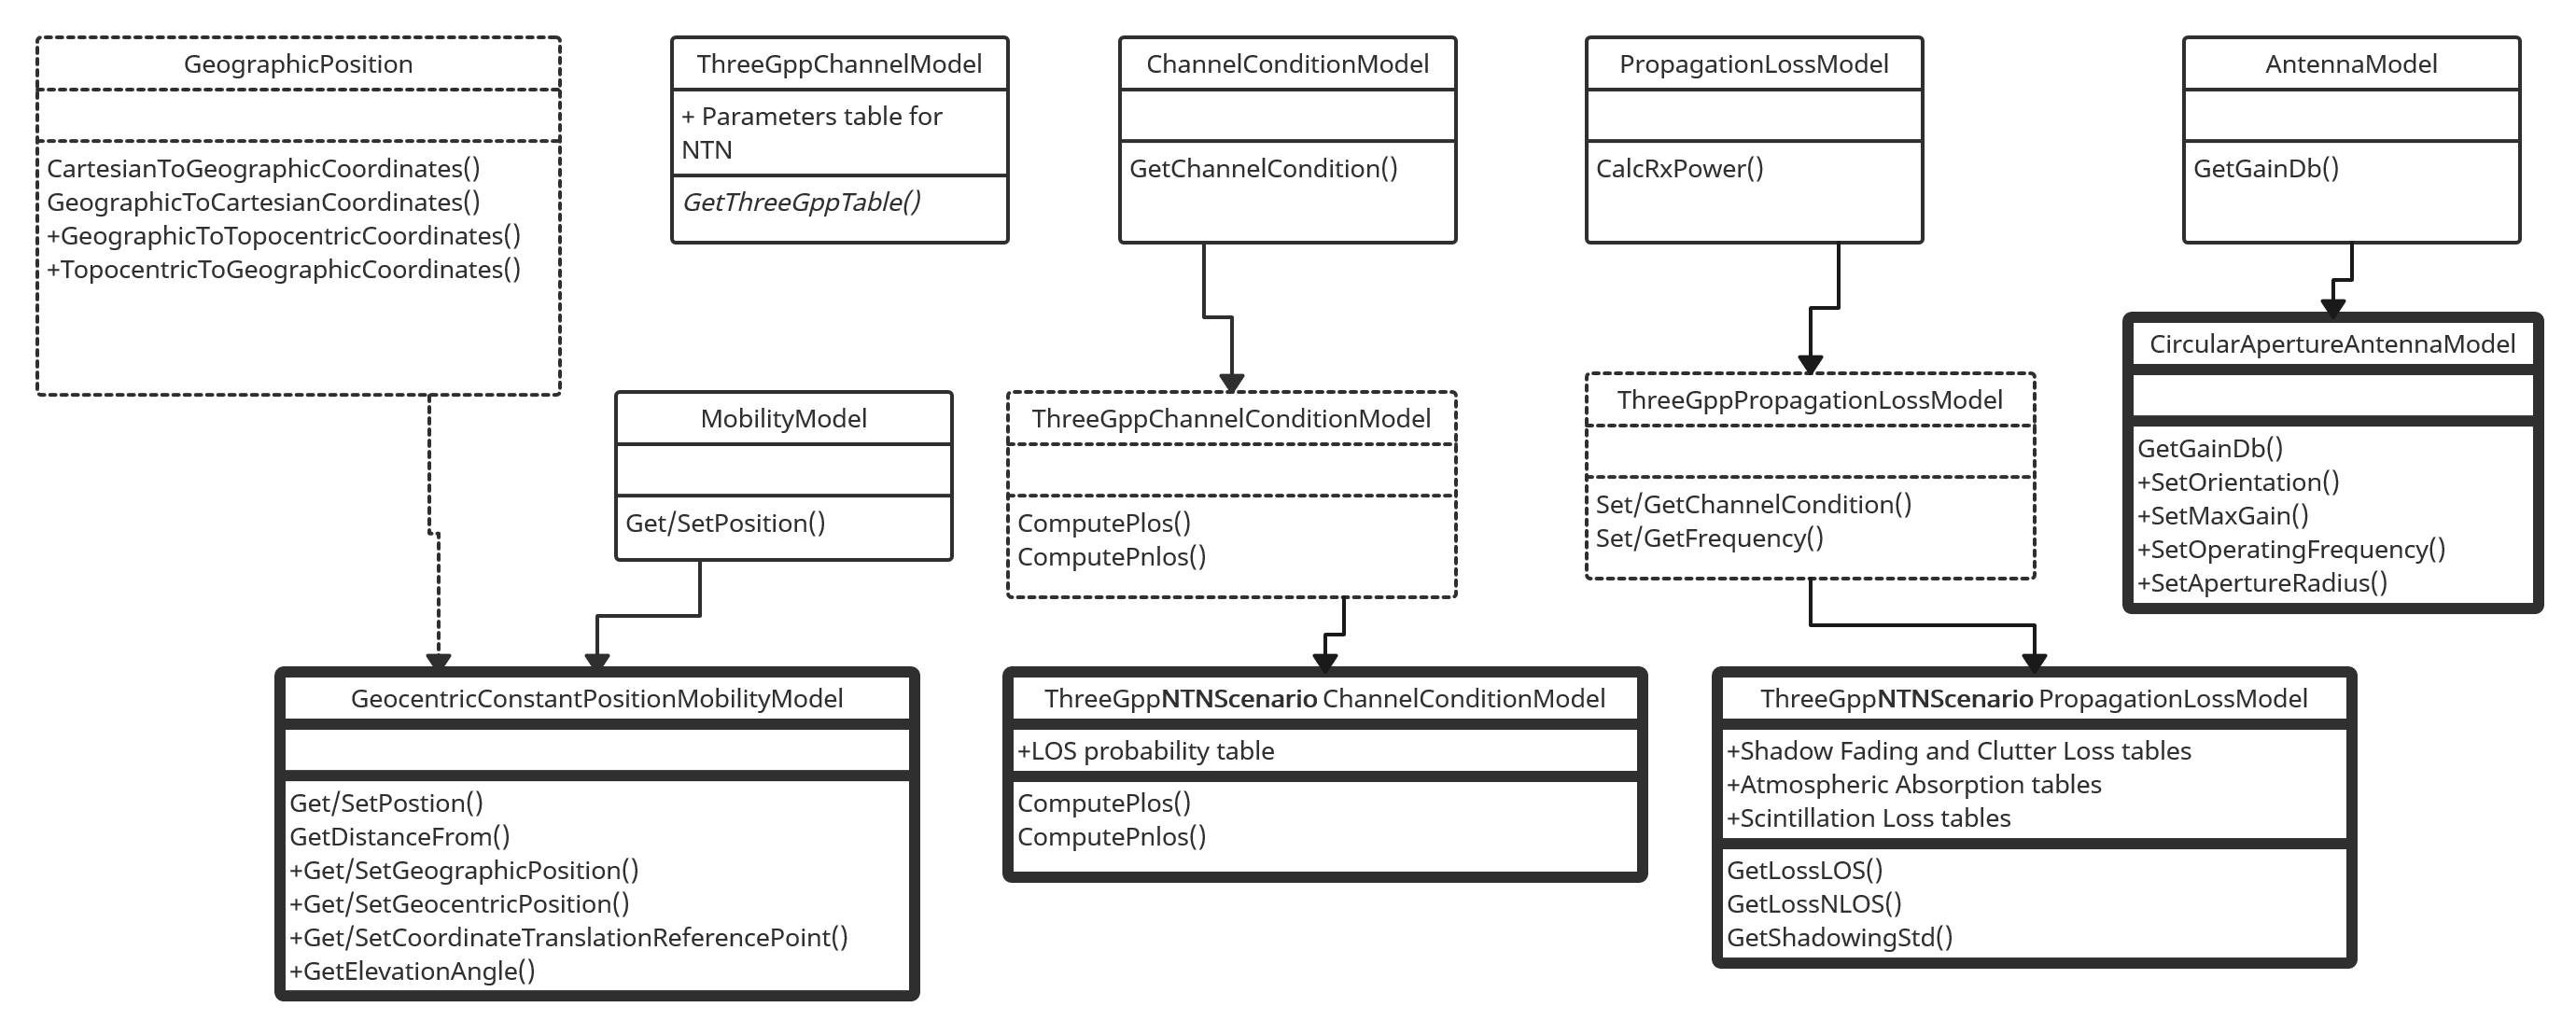
\includegraphics[width=1.3\textwidth, angle=90]{Figures/ChannelNtn/uml-diagram.png}
    \caption{Simplified UML diagram, which depicts the most significant changes which we introduced to ns-3. Bold outline classes represent the newly implemented ones, while dotted classes are pre-existing ones that have been modified.}
    \label{fig:ntn-uml}
\end{figure*}


\subsection{Coordinate System}
\label{sec:coord_model}
In general, the 3GPP defines a simple Cartesian coordinate system where the position of each node is uniquely described by a set of three values, $(x,y,z)$, where $x$ and $y$ define the ground plane, and $z$ represents the height of the node. 
While this model is accurate enough to describe scenarios where nodes are deployed at close distance (e.g., a few hundreds of meters), it is not for scenarios where end nodes are placed hundred (or thousands) of kilometers apart such as in the NTN environment. In this case, the Earth's curvature, as well as the elevation angle, play an important role.
Therefore, the \gls{3gpp} suggests to use a Geocentric Cartesian coordinate system (or \gls{ecef} system), where the position of a node is still described by three values $(x,y,z)$, but now the origin of the axes lays in the center of the Earth, which is modeled as a sphere of radius $R=6\,371$ km. 
The x-y plane defines the equatorial plane, with the x-axis pointing at 0-degree longitude, the y-axis pointing at 90-degree longitude, and the z-axis pointing at the geographical North Pole. 
Then, terrestrial nodes on the surface of the Earth are deployed so that $\sqrt{x^{2}+y^{2}+z^{2}}=R$, while aerial/space nodes flying/orbiting around the Earth are deployed so that $\sqrt{x^{2}+y^{2}+z^{2}}> R$.


\subsection{Implementation in ns-3}
\label{sec:implementation}
%The creation of the \gls{ntn} channel model follows the \gls{3gpp}~\cite{38811} guidelines presented in the previous section, which are considered a standard in the telecommunication landscape.  
The proposed ns-3 implementation of the 3GPP TR 38.811~\cite{38811} \gls{ntn} channel model is based upon the TR 38.901 model presented in~\cite{zugno20implementation}. Despite the fact that the newly introduced methods and classes are designed with the goal of introducing minimal changes to the existing ns-3 APIs, %, thus minimal change to existing classes is preferred.Nevertheless, 
some modifications to the existing code structure are still required. A schematic of these changes, which we make publicly available\footnote{\url{https://gitlab.com/mattiasandri/ns-3-ntn/-/tree/ntn-dev}}, can be found in Figure~\ref{fig:ntn-uml}.
The remainder of this section describes more in detail our implementation of the NTN channel model of~\cite{38811} in ns-3. 

%\subsection{ThreeGppChannelModel}
\subsubsection{Small-scale fading}
The most significant modifications to the pre-existing ns-3 classes concern the \texttt{Three\-Gpp\-Channel\-Model} class, which computes the small-scale propagation phenomena in the form of a complex channel matrix. Indeed, conversely from the procedure implemented in \cite{zugno20implementation}, in the \gls{ntn} channel model of~\cite{38811} most channel parameters depend on all the propagation scenario, \gls{los} condition, carrier frequency and elevation angle variables.  
To account for this, we store the small-scale fading parameters in a \emph{nested map}. The choice of this data-structure is motivated by the good trade-off between code efficiency and readability which it provides, considering that the possible combinations of the input parameters is particularly high, i.e., $144$.
%Taking into consideration four scenarios, two \gls{los} condition, two frequency band and nine elevation angle the final possible choices for a single parameters are 144. Given that the small scale parameters are more than 30 total values, a proper holding structure is needed to guarantee  bringing the choice to 

In particular, we change the signature of the \texttt{GetThreeGppTable()} method to include the \texttt{Mobility\-Model} instances of both transmitting and receiving nodes. In such a way, we account for the dependence of the small scale parameters with respect to the elevation angle, which the model of~\cite{38811} exhibits.
Finally, we include the required angular scaling factors for the propagation scenarios that have a lower number of clusters than the ones described in TR 38.901~\cite{TR38901}.

\subsubsection{Coordinate systems}
Instead of the coordinate system described in~\cite{TR38901}, the NTN channel model of~\cite{38811} considers the \emph{Geocentric Cartesian} (or \gls{ecef}) coordinate system.
We introduce this reference system in ns-3 via the \texttt{Geographic\-Positions} class, which provides methods to translate points represented using the coordinate system of~\cite{TR38901} to/from those of~\cite{38811}. 

Moreover, with usability in mind, we also implement a geographic coordinate system which allows ns-3 user to specify positions using the system of~\cite{38811} in a more convenient manner. This auxiliary reference system represents positions as points exhibiting a relative altitude from their projection on the surface of the Earth. That is to say, any location on, or possibly above, Earth is referenced by a longitude $\phi$, a latitude $\lambda$ and an altitude $h$. 
To this end, we implement in the \texttt{Geographic\-Positions} class the methods \texttt{Geographic\-To\-Topocentric\-Coordinates} and \texttt{Topocentric\-To\-Geographic\-Coordinates}, which can be used to translate positions between geocentric and non-geocentric geographic coordinate systems.

For the conversion between any of the newly introduced models, and the cartesian reference system of~\cite{TR38901}, we introduce a \emph{reference point} of translation between the two classes of coordinate systems, following the procedure outlined in \cite[Ch.~4]{coordinateconversion}.
%To conversion between a coordinate system that places a terminal on a location of the Earth to one in which the node position lays in a imaginary plane,  Coordinates that uses a reference point of origin are called \emph{topocentric coordinates}, or \gls{enu} coordinates.

\subsubsection{Channel condtion}
To model the channel condition for the \gls{ntn} propagation scenarios, we create the classes: 
\begin{itemize}
    \item \verb|ThreeGppNTNDenseUrbanChannelConditionMode|;
    \item \verb|ThreeGppNTNUrbanChannelConditionMode|;
    \item \verb|ThreeGppNTNSuburbanChannelConditionMode|; and
    \item \verb|ThreeGppNTNRuralChannelConditionMode|.
\end{itemize}
Each of these derives from the base class \texttt{Three\-Gpp\-Channel\-Condition\-Mode}|, which in turn implements the \texttt{Channel\-Condition\-Model} interface.

%The \texttt{ChannelCondition} class was developed to store the channel state, together with the interface \verb|ChannelConditionModel| that can be extended to implement any specific channel condition. The main method is \verb|GetChannelCondition|, which given two mobility models returns a pointer to the corresponding \verb|ChannelCondition|.
These channel condition classes interact with the remainder of the \texttt{spectrum} module as follows.
Whenever the \texttt{Get\-Channel\-Condition} method is called, the newly introduced NTN \texttt{Channel\-Condition\-Model} classes compute the channel state and cache it, along with its generation time. Then, the following calls to \texttt{Get\-Channel\-Condition} retrieve the previously stored value, if it has not expired. Otherwise, they compute a new \gls{los} condition. 

\subsubsection{Path loss and shadowing}
We implement the path loss and shadowing models of~\cite{38811} in four different classes, as depicted in Figure~\ref{fig:ntn-uml}. The latter extend the \texttt{Three\-Gpp\-Propagation\-Loss\-Model} class, which in turn implements the \texttt{Propagation\-Loss\-Model} interface.

The classes which implement this interface shall override the \texttt{Do\-Calc\-Rx\-Power}, returning the received power based on the positions of the communicating endpoints, and when considering frequency-flat phenomena only. 
In the case of the \gls{ntn} propagation scenarios of~\cite{38811}, these phenomena comprise the typical free space path loss, on top of tropospheric and ionospheric scintillation, shadow fading, clutter loss, and atmospheric absorption.

%The latter perform the power calculation using \verb|GetLossLos|, \verb|GetLossNlos|  and \verb|GetShadowing| to get the mean total pathloss. %Since the shadowing loss is modeled as a log-normal random variable, it's calculation require the \verb|GetShadowingStd| method, that returns the standard deviation value for a specific scenario. 

\subsubsection{Geocentric mobility models}
\label{sub:mobility}
%The creation of a , comes primarily from the need of calculating the elevation angle, which is essential in the estimation of many channel parameters. 
Along with the geographic coordinate systems, we implement a new mobility model, i.e., \texttt{Geocentric\-Constant\-Position\-Mobility\-Model}, which allows ns-3 users to position nodes using real world coordinates.
Specifically, the latter class stores positions via the variable \verb|m_position|, which specifies their geographic coordinates.

When using these mobility models, the position of a node can be retrieved (set) using the methods \texttt{Get\-Geographic\-Postion} (\texttt{Set\-Geographic\-Postion}) and \texttt{Get\-Geocentric\-Position} (\texttt{Set\-Geocentric\-Position}). In turn, these methods rely on the functionality provided by the class \texttt{Geographic\-Position} for translating between different coordinate systems. 

Notably, the conversion from geocentric cartesian or geographic coordinates, to the coordinate systems used by ns-3, uses by default the so-called reference point ``{Null Island}'' $(0,0,0)$. Nevertheless, ns-3 users are given the possibility of tuning this value by using the \texttt{Geocentric\-Constant\-Position\-Mobility\-Model} attribute \texttt{Set\-Coordinate\-Translation\-Reference\-Point}.

%The \verb|GeocentricConstantPositionMobilityModel| class is derived from the base class \verb|MobilityModel|, which imposes the presence of the \verb|Get/SetPosition()| methods, that are used to set and get the position of the object using planar Cartesian coordinates. 

%which implements the \texttt{Mobility\-Model} interface

%Hence, conversion to and from this coordinates is crucial to
%Additionally, the reference point for coordinates conversion can be set using, making the values obtained when using \verb|GetPosition()| more human readable.

\subsubsection{Antenna models}
The circular aperture reflector antenna model currently implemented in ns-3, i.e., \texttt{Parabolic\-Antenna\-Model}, is based on a parabolic approximation of the main lobe radiation pattern, as described in~\cite{parabolicantenna3gpp} and~\cite{parabolicantennamodel}. This simplification reduces the computational complexity of the field pattern calculation, by avoiding the Bessel functions evaluations that the circular aperture antenna would require, and using trigonometric approximations instead. 

As part of our contributions, we leverage the efficient implementation of the Bessel functions which has been introduced with C\texttt{++}17 to implement an exact circular aperture reflector antenna model. Specifically, we introduce this functionality extending the \texttt{Antenna\-Model} via the \texttt{Circular\-Aperture\-Antenna\-Model} class.
The latter allows ns-3 users to steer the pointing direction of the antenna via the \texttt{Set\-Orientation} and \texttt{Set\-Inclination} methods.
%, and overrides the \verb|GetGainDb| method of the base class using the proper field pattern calculation. 
Similarly, the operating frequency and the aperture radius %are essential parameters to correctly estimate the radiation pattern of a circular aperture antenna, thus 
can be tuned by using the methods \texttt{Set\-Operating\-Frequency} and \texttt{Set\-Aperture\-Radius}.

\subsection{Examples and Comparisons}
\label{sec:results-ntn}
In this section we validate the accuracy of our ns-3 module for the NTN channel, and compare simulation results with the calibration reported in TR 38.821 \cite{38821}. Furthermore, we provide numerical results to measure link-level and end-to-end performance (including throughput and packet drop ratio). We focus on satellites, even though the model is valid for different NTN scenarios.

\subsubsection{Link-Level Results}
\label{sub:ll}
While ns-3 enables system-level simulations, an evaluation of the link-level performance is still useful to validate the technical accuracy of our module. Hence, in this section we run link-level simulations to compare the calibration results from the 3GPP~\cite{38821} with results from our module. 

The 3GPP identifies 30 calibration study cases~\cite[Tab.~ 6.1.1.1-9]{38821}, which include a combination of different satellite orbits, frequency bands, and antenna configurations for the ground terminal. Link-level calibration results are reported in~\cite[Tab.~6.1.1.2]{38821}, including results for the \gls{fspl}, atmospheric loss (AL) and scintillation loss (SL), and the \gls{cnr}. 
Specifically, the \gls{cnr} is calculated as described in \cite[Section~6.1.3.1]{38821}. 

% Please add the following required packages to your document preamble:
% \usepackage{multirow}
\begin{table}[t!]
\caption{Link-level comparison between the 3GPP calibration results (``3GPP'') and those obtained in simulations (``Obtained''). Header acronyms: Free Space Path Loss (FSPL), Atmospheric Loss (AL), Scintillation Loss (SL), Carrier-to-Noise Ratio (CNR). All values are in dB.}
\label{tab:ll-comp}
\vspace{0.1cm}
\centering
\footnotesize
\begin{tabular}{|c|l|l|l|l|l|l|}
\hline
\textbf{SC} & \textbf{Tx} & \textbf{Source} & \textbf{FSPL} & \textbf{AL} & \textbf{SL} & \textbf{CNR} \\ \hline
\multirow{2}{*}{1} & \multirow{2}{*}{DL} & 3GPP & 210.6 & 1.2 & 1.1 & 11.6 \\
 &  & Obtained & 210.6 & 1.4 & 1.1 & 11.3 \\ \hline
\multirow{2}{*}{1} & \multirow{2}{*}{UL} & 3GPP & 214.1 & 1.1 & 1.1 & 0.5 \\
 &  & Obtained & 214.2 & 1.4 & 1.1 & 0.1 \\ \hline
\multirow{2}{*}{6} & \multirow{2}{*}{DL} & 3GPP & 179.1 & 0.5 & 0.3 & 8.5 \\
 &  & Obtained & 179.9 & 0.5 & 0.3 & 8.6 \\ \hline
\multirow{2}{*}{6} & \multirow{2}{*}{UL} & 3GPP & 182.6 & 0.5 & 0.3 & 18.4 \\
 &  & Obtained & 182.6 & 0.5 & 0.3 & 18.4 \\ \hline
\multirow{2}{*}{9} & \multirow{2}{*}{DL} & 3GPP & 159.1 & 0.1 & 2.2 & 6.6 \\
 &  & Obtained & 159.1 & 0.0 & 2.2 & 6.7 \\ \hline
\multirow{2}{*}{9} & \multirow{2}{*}{UL} & 3GPP & 159.1 & 0.1 & 2.2 & 2.8 \\
 &  & Obtained & 159.1 & 0.0 & 2.2 & 2.4 \\ \hline
\multirow{2}{*}{14} & \multirow{2}{*}{DL} & 3GPP & 164.5 & 0.1 & 2.2 & 7.2 \\
 &  & Obtained & 164.5 & 0.0 & 2.2 & 7.3 \\ \hline
\multirow{2}{*}{14} & \multirow{2}{*}{UL} & 3GPP & 164.5 & 0.1 & 2.2 & -2.6 \\
 &  & Obtained & 164.5 & 0.0 & 2.2 & -3 \\ \hline
\end{tabular}
\end{table}

For this comparison we selected four study cases, considering both \gls{ul} and \gls{dl} transmissions, that illustrate four representative NTN scenarios. Specifically: 
\begin{itemize}
    \item Study Case 1 (SC1): GEO satellite, 45 degrees of elevation, VSAT antenna for the ground terminal,	Ka-band.
    \item Study Case 6 (SC6): LEO satellite at 600 km, 90 degrees of elevation, VSAT antenna for the ground terminal,	Ka-band.
    \item Study Case 9 (SC9): LEO satellite at 600 km, 90 degrees of elevation, UPA antenna for the ground terminal,	S-band.
    \item Study Case 14 (SC14): LEO satellite at 1200 km, 90 degrees of elevation, UPA antenna for the ground terminal,	S-band.
\end{itemize}
The complete list of parameters used in the calibration can be found in \cite[Section 6.1]{38821}. 
In Tab.~\ref{tab:ll-comp} we report the calibration results (``3GPP'') and those from our simulations (``Obtained''). We can see that, despite some minor variations, numerical result are compatible under all metrics, thereby validating the accuracy of our module. 
As expected, the \gls{fspl} increases as the distance between the ground terminal and the satellite , as well as the carrier frequency, increase, due to the more severe effect of atmospheric losses. In particular, the impact of the carrier frequency is quite significant: for LEO satellites, for example, the \gls{fspl} grows from around 160 dB in the S-band (SC6) to around 180 dB in the Ka-band (SC9). In any case, we can see that, even considering long-rage GEO satellites in the Ka-band, the \gls{cnr} is large enough to support adequate levels of communication, especially in downlink. 
We shed light on two main trends. First, uplink communication is generally worse than downlink, except for SC6. This is reasonable, and due to the fact that ground terminals are more constrained in terms of power availability, capacity, and size (e.g., for antenna deployment).
Second, according to the 3GPP model, LEO satellites have more severe hardware constraints than GEO satellites (e.g., LEO's effective isotropic radiated power (EIRP) in the Ka-band is as low as 36 dBW, vs. 66 dBW for GEO): as a result, the CNR for SC6 is around 50\% lower than for SC1, which makes LEO communication more~difficult.

\begin{table}[t!]
    \caption{Simulation parameters.}
    \label{tab:frequency-test}
    \centering
    \footnotesize
    \begin{tabular}{|l|l|}
    \hline
    \textbf{Parameter} & \textbf{Value} \\ \hline
    {Frequency} & {20 GHz $\div$ 100 GHz} \\\hline
    {Satellite orbit} & {GEO} \\\hline
    {Satellite altitude} & {35\,786 km} \\\hline
    {Elevation angle} & {90 deg} \\\hline
    {Tx. mode} & {Downlink} \\\hline
    {Transmit power} & {37.5 dBm} \\\hline
    {Satellite antenna} & {Circular aperture (Gain: 58.5 dB)} \\\hline
    {Terminal antenna} & {VSAT (Gain: 39.7 dB)} \\\hline
     {Scenario} & {Suburban} \\\hline
    \end{tabular}
    \end{table}
    \begin{figure}[t]
        \centering 
    % These two commands set the width and height of the figure, respectively
        \setlength\fwidth{0.65\columnwidth}
        \setlength\fheight{0.28\columnwidth}
        % This file was created by matlab2tikz.
%
%The latest updates can be retrieved from
%  http://www.mathworks.com/matlabcentral/fileexchange/22022-matlab2tikz-matlab2tikz
%where you can also make suggestions and rate matlab2tikz.
%
\definecolor{mycolor1}{rgb}{0.00000,0.44700,0.74100}%
%
\begin{tikzpicture}

\begin{axis}[
% These scale the figure
width=\fwidth,
height=\fheight,
at={(0\fwidth,0\fheight)},
scale only axis,
xmin=20,
xmax=100,
xlabel style={font=\color{white!15!black}},
xlabel={Frequency [GHz]},
ymin=-180,
ymax=20,
xmajorgrids,
ymajorgrids,
ylabel style={font=\color{white!15!black}},
ylabel={SNR [dB]},
axis background/.style={fill=white},
legend style={legend cell align=left, align=left, draw=white!15!black}
]
\addplot [color=mycolor1, forget plot]
  table[row sep=crcr]{%
20.008	10.5123\\
20.016	10.4867\\
20.024	10.7442\\
20.032	10.7367\\
20.04	10.1959\\
20.048	10.2073\\
20.056	10.8154\\
20.064	10.8031\\
20.072	11.2108\\
20.08	11.209\\
20.088	11.7057\\
20.096	11.701\\
20.104	11.0678\\
20.112	11.0516\\
20.12	10.9702\\
20.128	10.9385\\
20.136	11.2418\\
20.144	11.2173\\
20.152	11.206\\
20.16	11.1815\\
20.168	11.5461\\
20.176	11.5518\\
20.184	10.9405\\
20.192	10.9428\\
20.2	11.0286\\
20.208	11.0427\\
20.216	11.0813\\
20.224	11.0521\\
20.232	10.9584\\
20.24	10.9507\\
20.248	11.7723\\
20.256	11.7646\\
20.264	11.0454\\
20.272	11.0436\\
20.28	10.4639\\
20.288	10.4836\\
20.296	11.3187\\
20.304	11.2943\\
20.312	10.2873\\
20.32	10.2916\\
20.328	10.7882\\
20.336	10.7884\\
20.344	9.92492\\
20.352	9.92662\\
20.36	10.3483\\
20.368	10.3545\\
20.376	11.009\\
20.384	11.0054\\
20.392	11.1526\\
20.4	11.1508\\
20.408	10.3361\\
20.416	10.3191\\
20.424	11.225\\
20.432	11.2243\\
20.44	10.8963\\
20.448	10.8971\\
20.456	11.2645\\
20.464	11.247\\
20.472	11.4795\\
20.48	11.4702\\
20.488	11.3567\\
20.496	11.3443\\
20.504	10.3899\\
20.512	10.3856\\
20.52	10.6781\\
20.528	10.7017\\
20.536	10.8787\\
20.544	10.8755\\
20.552	11.6201\\
20.56	11.606\\
20.568	10.3377\\
20.576	10.3453\\
20.584	10.6425\\
20.592	10.6463\\
20.6	10.3213\\
20.608	10.3057\\
20.616	10.7229\\
20.624	10.7194\\
20.632	10.7597\\
20.64	10.7449\\
20.648	10.9826\\
20.656	10.9813\\
20.664	9.05104\\
20.672	9.04939\\
20.68	11.2348\\
20.688	11.2404\\
20.696	10.4458\\
20.704	10.4425\\
20.712	10.2162\\
20.72	10.2213\\
20.728	10.7519\\
20.736	10.7467\\
20.744	10.1173\\
20.752	10.1121\\
20.76	10.5396\\
20.768	10.5596\\
20.776	10.6772\\
20.784	10.6616\\
20.792	9.97197\\
20.8	9.96844\\
20.808	10.5156\\
20.816	10.5016\\
20.824	11.2046\\
20.832	11.2\\
20.84	10.5054\\
20.848	10.5369\\
20.856	11.0901\\
20.864	11.0748\\
20.872	11.0991\\
20.88	11.1108\\
20.888	10.4719\\
20.896	10.4797\\
20.904	10.6503\\
20.912	10.6567\\
20.92	10.3903\\
20.928	10.3868\\
20.936	10.7622\\
20.944	10.7509\\
20.952	10.7245\\
20.96	10.7382\\
20.968	11.1522\\
20.976	11.1488\\
20.984	10.4648\\
20.992	10.443\\
21	10.6749\\
21.008	10.6918\\
21.016	10.4759\\
21.024	10.4743\\
21.032	11.4599\\
21.04	11.4564\\
21.048	10.6387\\
21.056	10.6297\\
21.064	10.9164\\
21.072	10.91\\
21.08	10.6319\\
21.088	10.6079\\
21.096	10.1598\\
21.104	10.1464\\
21.112	10.0564\\
21.12	10.0526\\
21.128	10.4851\\
21.136	10.4698\\
21.144	9.82559\\
21.152	9.84171\\
21.16	9.93749\\
21.168	9.9443\\
21.176	10.418\\
21.184	10.4051\\
21.192	9.62337\\
21.2	9.62671\\
21.208	9.9861\\
21.216	9.98872\\
21.224	9.60628\\
21.232	9.61202\\
21.24	10.1935\\
21.248	10.2012\\
21.256	10.7287\\
21.264	10.7109\\
21.272	10.4324\\
21.28	10.4344\\
21.288	11.6141\\
21.296	11.6113\\
21.304	10.778\\
21.312	10.7669\\
21.32	10.0092\\
21.328	10.0051\\
21.336	10.2562\\
21.344	10.2504\\
21.352	10.4992\\
21.36	10.5021\\
21.368	10.4814\\
21.376	10.4613\\
21.384	9.39598\\
21.392	9.38698\\
21.4	10.5181\\
21.408	10.5249\\
21.416	9.35026\\
21.424	9.35148\\
21.432	10.4971\\
21.44	10.4939\\
21.448	10.3968\\
21.456	10.3955\\
21.464	9.7915\\
21.472	9.76441\\
21.48	10.2074\\
21.488	10.1978\\
21.496	10.3273\\
21.504	10.2106\\
21.512	10.3506\\
21.52	10.3356\\
21.528	10.0437\\
21.536	10.0351\\
21.544	10.2203\\
21.552	10.2301\\
21.56	10.5713\\
21.568	10.5887\\
21.576	10.1388\\
21.584	10.1345\\
21.592	10.9492\\
21.6	10.9532\\
21.608	10.4696\\
21.616	10.4665\\
21.624	9.88562\\
21.632	9.88575\\
21.64	10.0903\\
21.648	10.071\\
21.656	10.1032\\
21.664	10.1273\\
21.672	9.4465\\
21.68	9.44581\\
21.688	9.95262\\
21.696	9.96612\\
21.704	10.7691\\
21.712	10.773\\
21.72	10.0635\\
21.728	10.066\\
21.736	9.37371\\
21.744	9.37201\\
21.752	10.0255\\
21.76	10.0226\\
21.768	10.1176\\
21.776	10.1027\\
21.784	10.2614\\
21.792	10.2589\\
21.8	10.4763\\
21.808	10.4863\\
21.816	10.1029\\
21.824	10.0791\\
21.832	10.0463\\
21.84	10.0511\\
21.848	9.0604\\
21.856	9.05722\\
21.864	9.86401\\
21.872	9.86898\\
21.88	9.90732\\
21.888	9.91464\\
21.896	9.98129\\
21.904	9.97921\\
21.912	10.7237\\
21.92	10.7167\\
21.928	10.2737\\
21.936	10.2783\\
21.944	9.78038\\
21.952	9.77333\\
21.96	10.0074\\
21.968	10.0181\\
21.976	10.7711\\
21.984	10.7674\\
21.992	9.17957\\
22	9.17644\\
22.008	10.206\\
22.016	10.1778\\
22.024	10.6259\\
22.032	10.6176\\
22.04	10.2794\\
22.048	10.2742\\
22.056	10.5664\\
22.064	10.5721\\
22.072	10.1365\\
22.08	10.1309\\
22.088	9.41883\\
22.096	9.41334\\
22.104	11.0285\\
22.112	11.0201\\
22.12	10.251\\
22.128	10.2547\\
22.136	9.91525\\
22.144	9.89325\\
22.152	10.2241\\
22.16	10.209\\
22.168	11.1068\\
22.176	11.1052\\
22.184	10.1712\\
22.192	10.1669\\
22.2	10.5264\\
22.208	10.532\\
22.216	9.91714\\
22.224	9.91458\\
22.232	9.23263\\
22.24	9.21693\\
22.248	10.2489\\
22.256	10.2653\\
22.264	10.0749\\
22.272	10.0861\\
22.28	9.44519\\
22.288	9.4511\\
22.296	10.2794\\
22.304	10.2871\\
22.312	8.77234\\
22.32	8.77082\\
22.328	9.79679\\
22.336	9.79205\\
22.344	10.2049\\
22.352	10.1872\\
22.36	9.85567\\
22.368	9.85775\\
22.376	10.2277\\
22.384	10.2426\\
22.392	9.11215\\
22.4	9.10901\\
22.408	9.93282\\
22.416	9.91284\\
22.424	10.3993\\
22.432	10.382\\
22.44	10.3192\\
22.448	10.3083\\
22.456	10.187\\
22.464	10.1914\\
22.472	9.76268\\
22.48	9.7631\\
22.488	9.32967\\
22.496	9.33483\\
22.504	9.49388\\
22.512	9.47761\\
22.52	10.2189\\
22.528	10.2184\\
22.536	9.6318\\
22.544	9.6431\\
22.552	10.0793\\
22.56	10.0929\\
22.568	10.2412\\
22.576	10.2378\\
22.584	10.76\\
22.592	10.7557\\
22.6	9.43508\\
22.608	9.42821\\
22.616	9.35618\\
22.624	9.36053\\
22.632	10.0405\\
22.64	10.037\\
22.648	9.3107\\
22.656	9.30927\\
22.664	9.24946\\
22.672	9.24397\\
22.68	9.13622\\
22.688	9.13693\\
22.696	9.67898\\
22.704	9.67768\\
22.712	10.7312\\
22.72	10.7303\\
22.728	9.76858\\
22.736	9.74913\\
22.744	9.7688\\
22.752	9.75677\\
22.76	9.75799\\
22.768	9.76085\\
22.776	9.54628\\
22.784	9.53892\\
22.792	10.1519\\
22.8	10.1633\\
22.808	9.72755\\
22.816	9.70964\\
22.824	9.40546\\
22.832	9.41067\\
22.84	9.6442\\
22.848	9.64105\\
22.856	9.32011\\
22.864	9.29373\\
22.872	10.2078\\
22.88	10.1973\\
22.888	10.442\\
22.896	10.4392\\
22.904	8.19408\\
22.912	8.19101\\
22.92	9.68977\\
22.928	9.68558\\
22.936	10.3511\\
22.944	10.358\\
22.952	9.51472\\
22.96	9.50335\\
22.968	9.10594\\
22.976	9.0836\\
22.984	10.3115\\
22.992	10.3111\\
23	9.18974\\
23.008	9.18875\\
23.016	8.30227\\
23.024	8.29849\\
23.032	9.8256\\
23.04	9.82203\\
23.048	9.10311\\
23.056	9.09584\\
23.064	8.99033\\
23.072	8.98344\\
23.08	9.3761\\
23.088	9.37835\\
23.096	9.76471\\
23.104	9.76839\\
23.112	9.33372\\
23.12	9.33137\\
23.128	8.63131\\
23.136	8.6307\\
23.144	9.21674\\
23.152	9.21342\\
23.16	9.08999\\
23.168	9.0876\\
23.176	9.8265\\
23.184	9.80721\\
23.192	9.02191\\
23.2	9.04075\\
23.208	9.54475\\
23.216	9.55944\\
23.224	9.5871\\
23.232	9.58432\\
23.24	9.39602\\
23.248	9.39039\\
23.256	9.35577\\
23.264	9.33433\\
23.272	8.36708\\
23.28	8.36738\\
23.288	9.80657\\
23.296	9.81503\\
23.304	8.43124\\
23.312	8.41208\\
23.32	9.83588\\
23.328	9.81113\\
23.336	9.50409\\
23.344	9.479\\
23.352	9.14824\\
23.36	9.15395\\
23.368	9.14932\\
23.376	9.16241\\
23.384	9.49254\\
23.392	9.48937\\
23.4	9.42013\\
23.408	9.43156\\
23.416	9.46854\\
23.424	9.44558\\
23.432	9.35126\\
23.44	9.35064\\
23.448	9.50002\\
23.456	9.49726\\
23.464	9.00971\\
23.472	8.99299\\
23.48	9.43618\\
23.488	9.4283\\
23.496	8.19508\\
23.504	8.19121\\
23.512	8.85304\\
23.52	8.85087\\
23.528	9.72387\\
23.536	9.72363\\
23.544	10.2259\\
23.552	10.2269\\
23.56	8.95003\\
23.568	8.94939\\
23.576	9.50455\\
23.584	9.51523\\
23.592	9.65282\\
23.6	9.65001\\
23.608	8.94816\\
23.616	8.94703\\
23.624	9.39183\\
23.632	9.41218\\
23.64	9.98998\\
23.648	9.98845\\
23.656	8.37881\\
23.664	8.3763\\
23.672	9.77881\\
23.68	9.77508\\
23.688	9.5577\\
23.696	9.56333\\
23.704	9.46033\\
23.712	9.47578\\
23.72	9.34042\\
23.728	9.3701\\
23.736	9.71998\\
23.744	9.71701\\
23.752	9.13322\\
23.76	9.14425\\
23.768	9.15352\\
23.776	9.14698\\
23.784	9.08055\\
23.792	9.09053\\
23.8	9.25915\\
23.808	9.26407\\
23.816	8.67945\\
23.824	8.65783\\
23.832	9.40366\\
23.84	9.4227\\
23.848	8.67301\\
23.856	8.67096\\
23.864	9.67686\\
23.872	9.65936\\
23.88	8.26562\\
23.888	8.26687\\
23.896	9.53683\\
23.904	9.5221\\
23.912	7.87759\\
23.92	7.876\\
23.928	9.99113\\
23.936	9.99539\\
23.944	9.33246\\
23.952	9.35184\\
23.96	9.65663\\
23.968	9.65017\\
23.976	9.49695\\
23.984	9.48386\\
23.992	8.30732\\
24	8.31234\\
24.008	9.19861\\
24.016	9.20399\\
24.024	9.1935\\
24.032	9.18845\\
24.04	9.0101\\
24.048	9.01933\\
24.056	9.66252\\
24.064	9.67387\\
24.072	8.87655\\
24.08	8.8697\\
24.088	9.62568\\
24.096	9.61304\\
24.104	10.3237\\
24.112	10.3182\\
24.12	9.48812\\
24.128	9.48489\\
24.136	10.0166\\
24.144	10.0043\\
24.152	8.78582\\
24.16	8.78283\\
24.168	7.91267\\
24.176	7.91036\\
24.184	9.32038\\
24.192	9.3076\\
24.2	9.3783\\
24.208	9.36038\\
24.216	9.03079\\
24.224	9.0218\\
24.232	7.97959\\
24.24	7.96763\\
24.248	8.71963\\
24.256	8.72012\\
24.264	8.85586\\
24.272	8.83315\\
24.28	8.27914\\
24.288	8.26175\\
24.296	9.1207\\
24.304	9.10245\\
24.312	9.1593\\
24.32	9.14066\\
24.328	9.49045\\
24.336	9.47718\\
24.344	9.32886\\
24.352	9.33497\\
24.36	9.32888\\
24.368	9.32995\\
24.376	9.61629\\
24.384	9.61339\\
24.392	8.88085\\
24.4	8.86975\\
24.408	9.38897\\
24.416	9.3847\\
24.424	8.9826\\
24.432	9.0141\\
24.44	9.08161\\
24.448	9.09441\\
24.456	8.3422\\
24.464	8.34892\\
24.472	8.92993\\
24.48	8.92382\\
24.488	9.16433\\
24.496	9.17356\\
24.504	7.87362\\
24.512	7.87284\\
24.52	9.00803\\
24.528	9.02259\\
24.536	8.47003\\
24.544	8.46842\\
24.552	9.17212\\
24.56	9.15791\\
24.568	10.1442\\
24.576	10.1418\\
24.584	9.38532\\
24.592	9.38261\\
24.6	8.95913\\
24.608	8.94491\\
24.616	9.94642\\
24.624	9.94338\\
24.632	8.95159\\
24.64	8.93956\\
24.648	8.81815\\
24.656	8.80123\\
24.664	8.44668\\
24.672	8.44272\\
24.68	9.68553\\
24.688	9.68878\\
24.696	8.04059\\
24.704	8.03796\\
24.712	9.56111\\
24.72	9.56301\\
24.728	8.91343\\
24.736	8.93247\\
24.744	9.28448\\
24.752	9.2762\\
24.76	8.29861\\
24.768	8.29596\\
24.776	8.78781\\
24.784	8.79592\\
24.792	9.64473\\
24.8	9.64124\\
24.808	7.83641\\
24.816	7.83221\\
24.824	9.27521\\
24.832	9.27387\\
24.84	8.77801\\
24.848	8.78178\\
24.856	8.68911\\
24.864	8.68144\\
24.872	8.77978\\
24.88	8.78511\\
24.888	9.02172\\
24.896	9.01715\\
24.904	8.77625\\
24.912	8.74768\\
24.92	9.08934\\
24.928	9.09475\\
24.936	8.70246\\
24.944	8.68141\\
24.952	8.15919\\
24.96	8.17023\\
24.968	8.74865\\
24.976	8.73615\\
24.984	9.20197\\
24.992	9.19906\\
25	8.70689\\
25.008	8.68337\\
25.016	8.00064\\
25.024	7.99761\\
25.032	8.17585\\
25.04	8.17606\\
25.048	8.66134\\
25.056	8.66658\\
25.064	9.29684\\
25.072	9.28522\\
25.08	9.01046\\
25.088	9.01736\\
25.096	8.5785\\
25.104	8.56833\\
25.112	8.75444\\
25.12	8.74305\\
25.128	8.58931\\
25.136	8.60378\\
25.144	7.92809\\
25.152	7.92578\\
25.16	8.91023\\
25.168	8.90616\\
25.176	8.78705\\
25.184	8.77166\\
25.192	8.69454\\
25.2	8.68972\\
25.208	8.75787\\
25.216	8.7637\\
25.224	8.75867\\
25.232	8.74586\\
25.24	9.2433\\
25.248	9.25577\\
25.256	9.20276\\
25.264	9.20026\\
25.272	9.7063\\
25.28	9.69689\\
25.288	8.68518\\
25.296	8.67221\\
25.304	8.66714\\
25.312	8.66939\\
25.32	9.16397\\
25.328	9.14631\\
25.336	8.19564\\
25.344	8.20727\\
25.352	8.77623\\
25.36	8.80206\\
25.368	9.54891\\
25.376	9.53516\\
25.384	8.66269\\
25.392	8.66052\\
25.4	9.41101\\
25.408	9.39886\\
25.416	8.02989\\
25.424	8.0256\\
25.432	8.53458\\
25.44	8.5412\\
25.448	8.28446\\
25.456	8.28904\\
25.464	8.31195\\
25.472	8.31806\\
25.48	8.59454\\
25.488	8.58037\\
25.496	7.77038\\
25.504	7.80401\\
25.512	8.57676\\
25.52	8.57958\\
25.528	8.97342\\
25.536	8.96991\\
25.544	8.05167\\
25.552	8.06329\\
25.56	9.15434\\
25.568	9.1513\\
25.576	8.83796\\
25.584	8.83409\\
25.592	7.86696\\
25.6	7.86378\\
25.608	7.96579\\
25.616	7.97196\\
25.624	8.73082\\
25.632	8.7365\\
25.64	8.52439\\
25.648	8.52013\\
25.656	8.73861\\
25.664	8.73602\\
25.672	9.02589\\
25.68	9.02406\\
25.688	8.71719\\
25.696	8.71446\\
25.704	8.18276\\
25.712	8.18\\
25.72	8.21262\\
25.728	8.22002\\
25.736	8.70919\\
25.744	8.71701\\
25.752	8.65062\\
25.76	8.64839\\
25.768	8.59821\\
25.776	8.62835\\
25.784	8.89757\\
25.792	8.89478\\
25.8	8.88684\\
25.808	8.89851\\
25.816	9.87217\\
25.824	9.86881\\
25.832	8.19437\\
25.84	8.21225\\
25.848	8.667\\
25.856	8.66729\\
25.864	8.6507\\
25.872	8.66102\\
25.88	8.50824\\
25.888	8.49234\\
25.896	8.94224\\
25.904	8.95082\\
25.912	8.8586\\
25.92	8.85602\\
25.928	8.56114\\
25.936	8.55918\\
25.944	9.47442\\
25.952	9.48412\\
25.96	7.80536\\
25.968	7.8106\\
25.976	8.76884\\
25.984	8.78345\\
25.992	7.66859\\
26	7.66413\\
26.008	9.30267\\
26.016	9.2995\\
26.024	8.07627\\
26.032	8.05525\\
26.04	8.54914\\
26.048	8.54693\\
26.056	7.9014\\
26.064	7.89879\\
26.072	8.66811\\
26.08	8.65699\\
26.088	9.15862\\
26.096	9.1601\\
26.104	8.62418\\
26.112	8.63537\\
26.12	8.2161\\
26.128	8.21526\\
26.136	8.91891\\
26.144	8.91712\\
26.152	8.76853\\
26.16	8.77497\\
26.168	8.51931\\
26.176	8.54291\\
26.184	8.57853\\
26.192	8.57188\\
26.2	9.79779\\
26.208	9.7952\\
26.216	8.56916\\
26.224	8.53936\\
26.232	9.00302\\
26.24	8.97781\\
26.248	7.53248\\
26.256	7.52023\\
26.264	8.501\\
26.272	8.48942\\
26.28	9.37217\\
26.288	9.37269\\
26.296	8.42414\\
26.304	8.42633\\
26.312	9.25099\\
26.32	9.24179\\
26.328	8.89064\\
26.336	8.88791\\
26.344	8.46524\\
26.352	8.48178\\
26.36	8.25216\\
26.368	8.25226\\
26.376	8.91457\\
26.384	8.92958\\
26.392	8.54663\\
26.4	8.55051\\
26.408	7.77515\\
26.416	7.76336\\
26.424	7.95603\\
26.432	7.95336\\
26.44	8.38874\\
26.448	8.37841\\
26.456	8.41345\\
26.464	8.41014\\
26.472	8.38758\\
26.48	8.37536\\
26.488	8.46812\\
26.496	8.44447\\
26.504	7.56212\\
26.512	7.55889\\
26.52	8.533\\
26.528	8.55384\\
26.536	8.2213\\
26.544	8.22493\\
26.552	7.97405\\
26.56	7.98721\\
26.568	8.54753\\
26.576	8.51832\\
26.584	8.4531\\
26.592	8.44206\\
26.6	8.87485\\
26.608	8.88071\\
26.616	8.5173\\
26.624	8.52259\\
26.632	8.1445\\
26.64	8.14328\\
26.648	7.60671\\
26.656	7.60403\\
26.664	8.53935\\
26.672	8.52512\\
26.68	8.17475\\
26.688	8.17013\\
26.696	8.39747\\
26.704	8.36491\\
26.712	8.49101\\
26.72	8.49221\\
26.728	8.37025\\
26.736	8.38337\\
26.744	7.65859\\
26.752	7.66416\\
26.76	8.23386\\
26.768	8.22728\\
26.776	8.21209\\
26.784	8.19975\\
26.792	8.31892\\
26.8	8.32231\\
26.808	8.40454\\
26.816	8.40972\\
26.824	8.53402\\
26.832	8.52486\\
26.84	8.82402\\
26.848	8.83396\\
26.856	8.48873\\
26.864	8.4855\\
26.872	8.13562\\
26.88	8.13284\\
26.888	8.56815\\
26.896	8.5648\\
26.904	8.41514\\
26.912	8.39851\\
26.92	8.50924\\
26.928	8.51572\\
26.936	8.03042\\
26.944	8.02074\\
26.952	8.35559\\
26.96	8.34242\\
26.968	7.93116\\
26.976	7.93015\\
26.984	7.35893\\
26.992	7.34658\\
27	8.38853\\
27.008	8.38506\\
27.016	8.67691\\
27.024	8.68485\\
27.032	8.32657\\
27.04	8.31255\\
27.048	8.17569\\
27.056	8.16265\\
27.064	7.3484\\
27.072	7.34812\\
27.08	7.89698\\
27.088	7.89898\\
27.096	8.41354\\
27.104	8.40939\\
27.112	8.05704\\
27.12	8.05263\\
27.128	8.97929\\
27.136	8.96665\\
27.144	8.27358\\
27.152	8.27549\\
27.16	8.91719\\
27.168	8.91197\\
27.176	8.22417\\
27.184	8.20129\\
27.192	8.38811\\
27.2	8.38589\\
27.208	7.42214\\
27.216	7.42933\\
27.224	8.0089\\
27.232	7.98957\\
27.24	7.40354\\
27.248	7.40333\\
27.256	7.9209\\
27.264	7.91415\\
27.272	7.03121\\
27.28	7.04049\\
27.288	8.2648\\
27.296	8.25847\\
27.304	8.67333\\
27.312	8.67172\\
27.32	8.09997\\
27.328	8.08361\\
27.336	7.29197\\
27.344	7.29032\\
27.352	8.99266\\
27.36	8.99623\\
27.368	8.87267\\
27.376	8.88236\\
27.384	8.15408\\
27.392	8.15893\\
27.4	8.32572\\
27.408	8.32141\\
27.416	8.42527\\
27.424	8.4177\\
27.432	8.99647\\
27.44	8.99081\\
27.448	7.66299\\
27.456	7.66\\
27.464	8.05258\\
27.472	8.04412\\
27.48	7.11735\\
27.488	7.10743\\
27.496	7.81343\\
27.504	7.89616\\
27.512	7.41842\\
27.52	7.41669\\
27.528	8.24511\\
27.536	8.23658\\
27.544	7.97346\\
27.552	7.99088\\
27.56	8.19203\\
27.568	8.18845\\
27.576	8.69393\\
27.584	8.68804\\
27.592	8.25716\\
27.6	8.23361\\
27.608	8.55678\\
27.616	8.54698\\
27.624	7.96257\\
27.632	7.96438\\
27.64	7.86693\\
27.648	7.86446\\
27.656	6.76895\\
27.664	6.76397\\
27.672	8.27457\\
27.68	8.25913\\
27.688	7.94488\\
27.696	7.92945\\
27.704	8.43688\\
27.712	8.4432\\
27.72	8.70216\\
27.728	8.68363\\
27.736	7.69278\\
27.744	7.70813\\
27.752	8.48144\\
27.76	8.47926\\
27.768	8.04262\\
27.776	8.06278\\
27.784	8.08609\\
27.792	8.07272\\
27.8	8.04978\\
27.808	8.03949\\
27.816	8.22561\\
27.824	8.24298\\
27.832	8.17249\\
27.84	8.16536\\
27.848	7.90626\\
27.856	7.90906\\
27.864	7.29693\\
27.872	7.2954\\
27.88	8.93015\\
27.888	8.92133\\
27.896	7.72577\\
27.904	7.7058\\
27.912	8.30403\\
27.92	8.31215\\
27.928	7.04581\\
27.936	7.04369\\
27.944	8.64762\\
27.952	8.66332\\
27.96	7.78593\\
27.968	7.78476\\
27.976	8.01169\\
27.984	8.0067\\
27.992	8.26712\\
28	8.2598\\
28.008	7.78232\\
28.016	7.78836\\
28.024	7.87431\\
28.032	7.84373\\
28.04	8.34945\\
28.048	8.32911\\
28.056	8.01366\\
28.064	8.01152\\
28.072	6.76766\\
28.08	6.75607\\
28.088	7.42154\\
28.096	7.4155\\
28.104	8.68734\\
28.112	8.6766\\
28.12	8.44946\\
28.128	8.44202\\
28.136	8.33324\\
28.144	8.33041\\
28.152	8.14187\\
28.16	8.14174\\
28.168	8.00299\\
28.176	8.00059\\
28.184	7.65624\\
28.192	7.64296\\
28.2	8.15684\\
28.208	8.14858\\
28.216	7.64511\\
28.224	7.64376\\
28.232	8.40702\\
28.24	8.40508\\
28.248	8.43191\\
28.256	8.41238\\
28.264	6.90162\\
28.272	6.9018\\
28.28	7.94642\\
28.288	7.93992\\
28.296	8.7819\\
28.304	8.7903\\
28.312	6.80799\\
28.32	6.80578\\
28.328	8.91342\\
28.336	8.91032\\
28.344	7.51944\\
28.352	7.52779\\
28.36	7.97924\\
28.368	7.97892\\
28.376	8.51546\\
28.384	8.49437\\
28.392	8.07647\\
28.4	8.07338\\
28.408	8.60062\\
28.416	8.60407\\
28.424	7.8805\\
28.432	7.89959\\
28.44	8.22665\\
28.448	8.23704\\
28.456	7.9162\\
28.464	7.89563\\
28.472	7.3896\\
28.48	7.36282\\
28.488	7.92634\\
28.496	7.94708\\
28.504	8.36944\\
28.512	8.38201\\
28.52	8.28476\\
28.528	8.28439\\
28.536	8.24759\\
28.544	8.2525\\
28.552	7.51202\\
28.56	7.51092\\
28.568	8.50042\\
28.576	8.49911\\
28.584	7.4846\\
28.592	7.4871\\
28.6	8.20284\\
28.608	8.19433\\
28.616	8.4032\\
28.624	8.39281\\
28.632	8.04506\\
28.64	8.04289\\
28.648	7.44294\\
28.656	7.43008\\
28.664	7.78208\\
28.672	7.76886\\
28.68	7.52513\\
28.688	7.5332\\
28.696	7.51879\\
28.704	7.49904\\
28.712	8.12559\\
28.72	8.10667\\
28.728	7.43618\\
28.736	7.43456\\
28.744	7.74396\\
28.752	7.74096\\
28.76	7.94212\\
28.768	7.92915\\
28.776	7.22866\\
28.784	7.22618\\
28.792	7.64117\\
28.8	7.63845\\
28.808	7.823\\
28.816	7.82782\\
28.824	7.92167\\
28.832	7.93388\\
28.84	8.71111\\
28.848	8.7085\\
28.856	8.26523\\
28.864	8.24561\\
28.872	6.92296\\
28.88	6.92036\\
28.888	8.32795\\
28.896	8.34328\\
28.904	8.0814\\
28.912	8.08487\\
28.92	8.055\\
28.928	8.04375\\
28.936	7.8689\\
28.944	7.85406\\
28.952	7.88\\
28.96	7.89782\\
28.968	7.61984\\
28.976	7.61745\\
28.984	7.20305\\
28.992	7.20149\\
29	6.97318\\
29.008	6.97242\\
29.016	8.42883\\
29.024	8.43601\\
29.032	7.42603\\
29.04	7.44197\\
29.048	7.61461\\
29.056	7.61177\\
29.064	8.87765\\
29.072	8.87371\\
29.08	7.47111\\
29.088	7.46271\\
29.096	8.53583\\
29.104	8.53429\\
29.112	8.09983\\
29.12	8.09936\\
29.128	7.77034\\
29.136	7.78623\\
29.144	7.77586\\
29.152	7.76636\\
29.16	7.77486\\
29.168	7.76838\\
29.176	8.51891\\
29.184	8.51316\\
29.192	7.31307\\
29.2	7.3381\\
29.208	7.88816\\
29.216	7.88343\\
29.224	7.54332\\
29.232	7.53735\\
29.24	7.79877\\
29.248	7.79876\\
29.256	7.27953\\
29.264	7.27602\\
29.272	7.84116\\
29.28	7.85826\\
29.288	7.72419\\
29.296	7.71644\\
29.304	7.23217\\
29.312	7.23329\\
29.32	8.20133\\
29.328	8.21805\\
29.336	6.99263\\
29.344	6.99296\\
29.352	7.3209\\
29.36	7.31633\\
29.368	8.14477\\
29.376	8.1449\\
29.384	7.55019\\
29.392	7.54379\\
29.4	8.00282\\
29.408	8.0154\\
29.416	7.75964\\
29.424	7.77154\\
29.432	8.57371\\
29.44	8.5772\\
29.448	7.33696\\
29.456	7.34331\\
29.464	8.03618\\
29.472	8.04953\\
29.48	6.27301\\
29.488	6.27054\\
29.496	7.95883\\
29.504	7.96391\\
29.512	7.07217\\
29.52	7.05498\\
29.528	7.94574\\
29.536	7.93099\\
29.544	7.92167\\
29.552	7.91725\\
29.56	7.77756\\
29.568	7.76761\\
29.576	7.11243\\
29.584	7.11106\\
29.592	8.13336\\
29.6	8.13186\\
29.608	7.72854\\
29.616	7.73056\\
29.624	7.71604\\
29.632	7.699\\
29.64	7.34316\\
29.648	7.34123\\
29.656	6.80985\\
29.664	6.81335\\
29.672	6.68277\\
29.68	6.69204\\
29.688	7.52653\\
29.696	7.53111\\
29.704	8.01709\\
29.712	8.00158\\
29.72	7.73961\\
29.728	7.73716\\
29.736	8.01679\\
29.744	7.99793\\
29.752	7.61979\\
29.76	7.63742\\
29.768	7.62363\\
29.776	7.60138\\
29.784	7.27268\\
29.792	7.28355\\
29.8	8.14812\\
29.808	8.14764\\
29.816	6.89768\\
29.824	6.88822\\
29.832	7.28337\\
29.84	7.30162\\
29.848	7.55842\\
29.856	7.53776\\
29.864	6.92663\\
29.872	6.93425\\
29.88	8.27673\\
29.888	8.27506\\
29.896	7.37935\\
29.904	7.37126\\
29.912	8.5603\\
29.92	8.55141\\
29.928	7.00674\\
29.936	7.00778\\
29.944	7.68187\\
29.952	7.67489\\
29.96	7.97432\\
29.968	7.97294\\
29.976	7.99327\\
29.984	7.99066\\
29.992	7.79312\\
30	7.81004\\
30.008	6.61397\\
30.016	6.61079\\
30.024	6.99017\\
30.032	6.98782\\
30.04	7.62931\\
30.048	7.63924\\
30.056	7.41969\\
30.064	7.41963\\
30.072	7.74405\\
30.08	7.75961\\
30.088	8.08611\\
30.096	8.10177\\
30.104	7.57116\\
30.112	7.58179\\
30.12	7.58732\\
30.128	7.6044\\
30.136	6.87099\\
30.144	6.87307\\
30.152	6.89829\\
30.16	6.91288\\
30.168	7.09617\\
30.176	7.09274\\
30.184	7.51132\\
30.192	7.49993\\
30.2	6.33867\\
30.208	6.34675\\
30.216	7.19608\\
30.224	7.1696\\
30.232	7.32374\\
30.24	7.35134\\
30.248	7.2427\\
30.256	7.22564\\
30.264	7.39938\\
30.272	7.37591\\
30.28	7.1425\\
30.288	7.14149\\
30.296	7.52182\\
30.304	7.53587\\
30.312	7.47897\\
30.32	7.46106\\
30.328	7.79408\\
30.336	7.79149\\
30.344	8.222\\
30.352	8.22712\\
30.36	7.47283\\
30.368	7.48452\\
30.376	7.00281\\
30.384	7.01246\\
30.392	6.67999\\
30.4	6.67488\\
30.408	7.28517\\
30.416	7.29033\\
30.424	7.51953\\
30.432	7.51113\\
30.44	6.31704\\
30.448	6.31779\\
30.456	7.56362\\
30.464	7.57008\\
30.472	6.97411\\
30.48	6.97241\\
30.488	6.5258\\
30.496	6.52501\\
30.504	7.34849\\
30.512	7.33823\\
30.52	7.67577\\
30.528	7.67238\\
30.536	7.88748\\
30.544	7.88039\\
30.552	8.05416\\
30.56	8.05723\\
30.568	7.49075\\
30.576	7.46178\\
30.584	7.01356\\
30.592	7.01043\\
30.6	6.66209\\
30.608	6.66264\\
30.616	6.59182\\
30.624	6.58786\\
30.632	6.83385\\
30.64	6.83392\\
30.648	7.09793\\
30.656	7.10147\\
30.664	7.42413\\
30.672	7.4286\\
30.68	6.79275\\
30.688	6.78546\\
30.696	6.97414\\
30.704	6.98259\\
30.712	7.87598\\
30.72	7.85137\\
30.728	8.08906\\
30.736	8.09794\\
30.744	7.425\\
30.752	7.41126\\
30.76	6.76885\\
30.768	6.76601\\
30.776	7.62768\\
30.784	7.60859\\
30.792	7.70211\\
30.8	7.70079\\
30.808	6.42344\\
30.816	6.42223\\
30.824	7.40699\\
30.832	7.37981\\
30.84	6.51659\\
30.848	6.5145\\
30.856	6.70293\\
30.864	6.70025\\
30.872	7.27742\\
30.88	7.26106\\
30.888	6.99714\\
30.896	6.98392\\
30.904	6.37154\\
30.912	6.37094\\
30.92	6.85928\\
30.928	6.85485\\
30.936	7.27033\\
30.944	7.29401\\
30.952	7.64309\\
30.96	7.65879\\
30.968	7.47703\\
30.976	7.47558\\
30.984	6.62222\\
30.992	6.62052\\
31	8.22046\\
31.008	8.2167\\
31.016	6.90368\\
31.024	6.89297\\
31.032	6.39584\\
31.04	6.39049\\
31.048	7.15752\\
31.056	7.1739\\
31.064	6.17925\\
31.072	6.19063\\
31.08	7.18078\\
31.088	7.20961\\
31.096	6.70053\\
31.104	6.69411\\
31.112	6.8643\\
31.12	6.84484\\
31.128	7.04252\\
31.136	7.02413\\
31.144	7.14166\\
31.152	7.12237\\
31.16	7.48371\\
31.168	7.4733\\
31.176	7.4817\\
31.184	7.46673\\
31.192	7.17928\\
31.2	7.18658\\
31.208	6.83954\\
31.216	6.83733\\
31.224	6.75048\\
31.232	6.73483\\
31.24	7.29577\\
31.248	7.27191\\
31.256	7.23562\\
31.264	7.22871\\
31.272	7.59101\\
31.28	7.59164\\
31.288	6.99041\\
31.296	6.98763\\
31.304	7.3023\\
31.312	7.30146\\
31.32	7.96099\\
31.328	7.94774\\
31.336	7.32652\\
31.344	7.32884\\
31.352	7.48001\\
31.36	7.47784\\
31.368	7.18265\\
31.376	7.20928\\
31.384	8.04\\
31.392	8.03627\\
31.4	7.10077\\
31.408	7.08766\\
31.416	7.06954\\
31.424	7.06309\\
31.432	7.4379\\
31.44	7.43476\\
31.448	7.0012\\
31.456	6.99455\\
31.464	7.15816\\
31.472	7.15825\\
31.48	7.39188\\
31.488	7.38756\\
31.496	6.71183\\
31.504	6.70472\\
31.512	7.61917\\
31.52	7.62686\\
31.528	7.66407\\
31.536	7.65958\\
31.544	6.98215\\
31.552	6.96719\\
31.56	7.70888\\
31.568	7.7087\\
31.576	8.17979\\
31.584	8.17793\\
31.592	6.93506\\
31.6	6.947\\
31.608	7.17715\\
31.616	7.18101\\
31.624	6.68303\\
31.632	6.66727\\
31.64	7.6397\\
31.648	7.64363\\
31.656	7.55868\\
31.664	7.5623\\
31.672	6.63088\\
31.68	6.64831\\
31.688	7.00514\\
31.696	6.98991\\
31.704	7.06654\\
31.712	7.04566\\
31.72	7.8796\\
31.728	7.86621\\
31.736	7.28023\\
31.744	7.27275\\
31.752	7.89176\\
31.76	7.87855\\
31.768	7.12977\\
31.776	7.13371\\
31.784	6.77081\\
31.792	6.76072\\
31.8	7.20611\\
31.808	7.20285\\
31.816	7.58971\\
31.824	7.56705\\
31.832	7.16415\\
31.84	7.15338\\
31.848	6.93115\\
31.856	6.92301\\
31.864	7.10991\\
31.872	7.12652\\
31.88	6.14708\\
31.888	6.14384\\
31.896	6.77848\\
31.904	6.78242\\
31.912	7.45527\\
31.92	7.45174\\
31.928	7.36787\\
31.936	7.36482\\
31.944	6.96071\\
31.952	6.93844\\
31.96	7.03462\\
31.968	7.02896\\
31.976	5.90883\\
31.984	5.90104\\
31.992	6.90456\\
32	6.90963\\
32.008	6.87683\\
32.016	6.87861\\
32.024	6.34845\\
32.032	6.3365\\
32.04	6.98355\\
32.048	6.98184\\
32.056	6.92524\\
32.064	6.91048\\
32.072	6.91286\\
32.08	6.91525\\
32.088	5.69132\\
32.096	5.69167\\
32.104	6.92558\\
32.112	6.92471\\
32.12	7.17737\\
32.128	7.18485\\
32.136	6.54904\\
32.144	6.53471\\
32.152	7.69914\\
32.16	7.69261\\
32.168	6.96425\\
32.176	6.9803\\
32.184	7.70234\\
32.192	7.69971\\
32.2	6.15352\\
32.208	6.15052\\
32.216	7.26337\\
32.224	7.26853\\
32.232	7.2161\\
32.24	7.21403\\
32.248	7.10408\\
32.256	7.08272\\
32.264	7.04535\\
32.272	7.06134\\
32.28	6.80129\\
32.288	6.80949\\
32.296	6.90679\\
32.304	6.91307\\
32.312	6.4642\\
32.32	6.47147\\
32.328	7.27328\\
32.336	7.26569\\
32.344	6.52172\\
32.352	6.50881\\
32.36	6.91542\\
32.368	6.92554\\
32.376	6.62898\\
32.384	6.61647\\
32.392	7.78047\\
32.4	7.78358\\
32.408	6.8207\\
32.416	6.81443\\
32.424	6.74272\\
32.432	6.7474\\
32.44	7.08072\\
32.448	7.06948\\
32.456	6.76841\\
32.464	6.77233\\
32.472	7.30052\\
32.48	7.29791\\
32.488	5.90164\\
32.496	5.91042\\
32.504	7.03493\\
32.512	7.03415\\
32.52	7.12968\\
32.528	7.14455\\
32.536	7.66146\\
32.544	7.65002\\
32.552	7.25528\\
32.56	7.25298\\
32.568	6.82326\\
32.576	6.82009\\
32.584	5.72351\\
32.592	5.72954\\
32.6	6.35665\\
32.608	6.35743\\
32.616	6.62566\\
32.624	6.65778\\
32.632	5.90639\\
32.64	5.90368\\
32.648	6.25717\\
32.656	6.25343\\
32.664	7.07515\\
32.672	7.07103\\
32.68	6.11236\\
32.688	6.11203\\
32.696	6.87867\\
32.704	6.89483\\
32.712	6.35597\\
32.72	6.34511\\
32.728	7.4704\\
32.736	7.47009\\
32.744	6.20506\\
32.752	6.20248\\
32.76	6.66666\\
32.768	6.67574\\
32.776	5.94353\\
32.784	5.94092\\
32.792	6.62971\\
32.8	6.62319\\
32.808	5.85189\\
32.816	5.84933\\
32.824	7.02108\\
32.832	7.02019\\
32.84	6.42522\\
32.848	6.42338\\
32.856	6.83227\\
32.864	6.81005\\
32.872	6.88745\\
32.88	6.88576\\
32.888	6.54961\\
32.896	6.56866\\
32.904	6.25536\\
32.912	6.23634\\
32.92	6.76227\\
32.928	6.77729\\
32.936	6.96264\\
32.944	6.94514\\
32.952	6.71164\\
32.96	6.70161\\
32.968	6.2322\\
32.976	6.21917\\
32.984	5.35341\\
32.992	5.35141\\
33	6.41458\\
33.008	6.4155\\
33.016	6.74246\\
33.024	6.72323\\
33.032	7.19581\\
33.04	7.19266\\
33.048	6.77299\\
33.056	6.77617\\
33.064	6.87156\\
33.072	6.8559\\
33.08	6.84362\\
33.088	6.84252\\
33.096	6.33795\\
33.104	6.34544\\
33.112	7.43178\\
33.12	7.43381\\
33.128	6.61248\\
33.136	6.61767\\
33.144	6.65106\\
33.152	6.66146\\
33.16	6.65534\\
33.168	6.66708\\
33.176	7.20817\\
33.184	7.20918\\
33.192	6.61025\\
33.2	6.6113\\
33.208	7.59985\\
33.216	7.60687\\
33.224	6.47247\\
33.232	6.4709\\
33.24	6.90987\\
33.248	6.90497\\
33.256	6.98948\\
33.264	6.98575\\
33.272	7.27759\\
33.28	7.2694\\
33.288	6.83747\\
33.296	6.82894\\
33.304	7.28988\\
33.312	7.2873\\
33.32	6.76681\\
33.328	6.7569\\
33.336	7.97099\\
33.344	7.97096\\
33.352	6.93233\\
33.36	6.92844\\
33.368	6.94288\\
33.376	6.93641\\
33.384	6.50351\\
33.392	6.50561\\
33.4	6.96787\\
33.408	6.9722\\
33.416	6.74599\\
33.424	6.74344\\
33.432	6.60827\\
33.44	6.60554\\
33.448	6.52199\\
33.456	6.5337\\
33.464	6.56555\\
33.472	6.54869\\
33.48	6.61386\\
33.488	6.6049\\
33.496	6.38851\\
33.504	6.37813\\
33.512	7.34032\\
33.52	7.33816\\
33.528	6.62103\\
33.536	6.61717\\
33.544	6.54145\\
33.552	6.53185\\
33.56	5.57201\\
33.568	5.56953\\
33.576	5.09165\\
33.584	5.08735\\
33.592	7.01633\\
33.6	7.02009\\
33.608	6.36246\\
33.616	6.35984\\
33.624	6.13721\\
33.632	6.13477\\
33.64	6.50118\\
33.648	6.52292\\
33.656	6.76685\\
33.664	6.76128\\
33.672	5.58268\\
33.68	5.56919\\
33.688	7.05296\\
33.696	7.05076\\
33.704	6.44599\\
33.712	6.43482\\
33.72	6.28065\\
33.728	6.28327\\
33.736	5.82525\\
33.744	5.82343\\
33.752	6.44754\\
33.76	6.46771\\
33.768	6.45678\\
33.776	6.45117\\
33.784	7.28909\\
33.792	7.27573\\
33.8	6.23415\\
33.808	6.24004\\
33.816	5.96508\\
33.824	5.94892\\
33.832	5.8613\\
33.84	5.86975\\
33.848	5.48706\\
33.856	5.4844\\
33.864	5.71086\\
33.872	5.70741\\
33.88	6.23522\\
33.888	6.2215\\
33.896	6.5356\\
33.904	6.51194\\
33.912	5.02296\\
33.92	5.02089\\
33.928	7.03826\\
33.936	7.04476\\
33.944	6.61607\\
33.952	6.63018\\
33.96	6.13042\\
33.968	6.1465\\
33.976	6.26829\\
33.984	6.27655\\
33.992	6.32593\\
34	6.30662\\
34.008	7.25629\\
34.016	7.2428\\
34.024	5.5353\\
34.032	5.52987\\
34.04	5.98781\\
34.048	6.00066\\
34.056	6.22205\\
34.064	6.22962\\
34.072	6.00177\\
34.08	5.97732\\
34.088	6.85636\\
34.096	6.85354\\
34.104	5.87671\\
34.112	5.89697\\
34.12	6.47694\\
34.128	6.46269\\
34.136	6.40363\\
34.144	6.41069\\
34.152	6.20518\\
34.16	6.20196\\
34.168	7.36359\\
34.176	7.36169\\
34.184	5.77572\\
34.192	5.79158\\
34.2	6.22451\\
34.208	6.2148\\
34.216	5.97627\\
34.224	5.99823\\
34.232	6.06069\\
34.24	6.045\\
34.248	4.91889\\
34.256	4.91676\\
34.264	6.04535\\
34.272	6.04668\\
34.28	6.88301\\
34.288	6.88133\\
34.296	5.1809\\
34.304	5.16662\\
34.312	6.34313\\
34.32	6.32755\\
34.328	7.07414\\
34.336	7.07229\\
34.344	6.94759\\
34.352	6.94505\\
34.36	7.38413\\
34.368	7.38193\\
34.376	5.38688\\
34.384	5.38939\\
34.392	7.06391\\
34.4	7.06424\\
34.408	5.94224\\
34.416	5.94033\\
34.424	5.89534\\
34.432	5.87899\\
34.44	6.32127\\
34.448	6.29134\\
34.456	6.53689\\
34.464	6.53383\\
34.472	5.82152\\
34.48	5.81912\\
34.488	6.45395\\
34.496	6.44365\\
34.504	6.23026\\
34.512	6.22183\\
34.52	6.24073\\
34.528	6.24514\\
34.536	6.04013\\
34.544	6.02864\\
34.552	6.47566\\
34.56	6.47763\\
34.568	6.03607\\
34.576	6.03668\\
34.584	6.16878\\
34.592	6.1858\\
34.6	6.06161\\
34.608	6.08282\\
34.616	5.44658\\
34.624	5.44458\\
34.632	6.26013\\
34.64	6.25524\\
34.648	5.68801\\
34.656	5.67567\\
34.664	5.74642\\
34.672	5.75861\\
34.68	6.40221\\
34.688	6.40106\\
34.696	5.95799\\
34.704	5.9416\\
34.712	6.14508\\
34.72	6.14175\\
34.728	6.49668\\
34.736	6.50092\\
34.744	6.22447\\
34.752	6.21375\\
34.76	6.64911\\
34.768	6.64309\\
34.776	5.47849\\
34.784	5.4874\\
34.792	6.79338\\
34.8	6.7878\\
34.808	6.25591\\
34.816	6.22925\\
34.824	4.9709\\
34.832	4.96739\\
34.84	6.16729\\
34.848	6.1656\\
34.856	6.44899\\
34.864	6.44831\\
34.872	5.90045\\
34.88	5.92057\\
34.888	5.39125\\
34.896	5.40062\\
34.904	6.1618\\
34.912	6.1533\\
34.92	5.87655\\
34.928	5.86071\\
34.936	6.61345\\
34.944	6.60082\\
34.952	6.19036\\
34.96	6.1857\\
34.968	6.85695\\
34.976	6.85338\\
34.984	6.12167\\
34.992	6.10771\\
35	6.206\\
35.008	6.21857\\
35.016	6.0771\\
35.024	6.07999\\
35.032	6.22654\\
35.04	6.21044\\
35.048	6.3816\\
35.056	6.39471\\
35.064	5.87843\\
35.072	5.87668\\
35.08	6.16102\\
35.088	6.16404\\
35.096	6.94904\\
35.104	6.93891\\
35.112	5.84219\\
35.12	5.83914\\
35.128	6.14435\\
35.136	6.13886\\
35.144	5.61375\\
35.152	5.62032\\
35.16	6.3977\\
35.168	6.39627\\
35.176	6.23294\\
35.184	6.24681\\
35.192	5.94434\\
35.2	5.93603\\
35.208	6.04512\\
35.216	6.03568\\
35.224	6.05624\\
35.232	6.04799\\
35.24	6.14158\\
35.248	6.14234\\
35.256	5.35986\\
35.264	5.36255\\
35.272	6.65734\\
35.28	6.65472\\
35.288	5.89735\\
35.296	5.89474\\
35.304	6.19692\\
35.312	6.18376\\
35.32	7.24615\\
35.328	7.24951\\
35.336	6.07508\\
35.344	6.08149\\
35.352	5.64023\\
35.36	5.6438\\
35.368	6.05326\\
35.376	6.02456\\
35.384	5.52946\\
35.392	5.51356\\
35.4	5.94448\\
35.408	5.96782\\
35.416	6.26614\\
35.424	6.26289\\
35.432	5.78386\\
35.44	5.79179\\
35.448	6.0926\\
35.456	6.08885\\
35.464	6.53419\\
35.472	6.5347\\
35.48	4.35066\\
35.488	4.35195\\
35.496	5.99001\\
35.504	5.95614\\
35.512	6.14275\\
35.52	6.16232\\
35.528	4.46623\\
35.536	4.4662\\
35.544	6.02629\\
35.552	6.04633\\
35.56	5.73256\\
35.568	5.73597\\
35.576	6.58316\\
35.584	6.56554\\
35.592	6.23515\\
35.6	6.25267\\
35.608	6.63899\\
35.616	6.62438\\
35.624	6.07582\\
35.632	6.0838\\
35.64	4.67608\\
35.648	4.67704\\
35.656	6.12311\\
35.664	6.12069\\
35.672	4.8137\\
35.68	4.80849\\
35.688	6.0722\\
35.696	6.05331\\
35.704	5.90461\\
35.712	5.93317\\
35.72	5.24197\\
35.728	5.23112\\
35.736	6.8559\\
35.744	6.86054\\
35.752	6.13709\\
35.76	6.12649\\
35.768	5.54168\\
35.776	5.54976\\
35.784	5.69642\\
35.792	5.69675\\
35.8	5.35336\\
35.808	5.35996\\
35.816	5.10173\\
35.824	5.09873\\
35.832	6.04743\\
35.84	6.03866\\
35.848	5.2983\\
35.856	5.30208\\
35.864	5.70029\\
35.872	5.69508\\
35.88	5.97571\\
35.888	5.96751\\
35.896	5.8337\\
35.904	5.82529\\
35.912	6.05977\\
35.92	6.03496\\
35.928	5.71035\\
35.936	5.71736\\
35.944	5.80744\\
35.952	5.81486\\
35.96	6.01078\\
35.968	5.99973\\
35.976	5.06118\\
35.984	5.07449\\
35.992	5.84729\\
36	5.84151\\
36.008	5.14746\\
36.016	5.14732\\
36.024	5.81581\\
36.032	5.81508\\
36.04	6.13242\\
36.048	6.13829\\
36.056	6.14367\\
36.064	6.14019\\
36.072	6.25261\\
36.08	6.26534\\
36.088	5.57208\\
36.096	5.56831\\
36.104	6.39005\\
36.112	6.3893\\
36.12	5.88433\\
36.128	5.8858\\
36.136	5.77657\\
36.144	5.77488\\
36.152	6.05627\\
36.16	6.05623\\
36.168	5.91248\\
36.176	5.91094\\
36.184	5.0858\\
36.192	5.0839\\
36.2	6.61148\\
36.208	6.60053\\
36.216	5.80131\\
36.224	5.80936\\
36.232	5.93282\\
36.24	5.92612\\
36.248	5.63118\\
36.256	5.6343\\
36.264	4.51629\\
36.272	4.51435\\
36.28	6.62542\\
36.288	6.61273\\
36.296	5.80712\\
36.304	5.83732\\
36.312	6.21961\\
36.32	6.19977\\
36.328	6.74987\\
36.336	6.75183\\
36.344	6.33194\\
36.352	6.32347\\
36.36	6.18559\\
36.368	6.1837\\
36.376	5.22126\\
36.384	5.21824\\
36.392	5.87226\\
36.4	5.87842\\
36.408	6.10331\\
36.416	6.10124\\
36.424	5.51671\\
36.432	5.52111\\
36.44	6.12582\\
36.448	6.1268\\
36.456	5.95238\\
36.464	5.95077\\
36.472	4.40423\\
36.48	4.395\\
36.488	5.84154\\
36.496	5.83315\\
36.504	5.12674\\
36.512	5.12745\\
36.52	5.80903\\
36.528	5.7915\\
36.536	6.14603\\
36.544	6.13031\\
36.552	6.37111\\
36.56	6.36037\\
36.568	5.53611\\
36.576	5.53081\\
36.584	5.60109\\
36.592	5.61349\\
36.6	5.70724\\
36.608	5.6958\\
36.616	4.49293\\
36.624	4.49156\\
36.632	5.10149\\
36.64	5.1072\\
36.648	5.27938\\
36.656	5.28308\\
36.664	5.99236\\
36.672	5.99199\\
36.68	5.78952\\
36.688	5.79232\\
36.696	5.71438\\
36.704	5.69847\\
36.712	5.46472\\
36.72	5.46391\\
36.728	5.41785\\
36.736	5.43481\\
36.744	6.09224\\
36.752	6.10608\\
36.76	5.59743\\
36.768	5.59584\\
36.776	6.02213\\
36.784	6.02834\\
36.792	4.95274\\
36.8	4.95699\\
36.808	6.02267\\
36.816	6.00738\\
36.824	4.62652\\
36.832	4.62293\\
36.84	6.13612\\
36.848	6.11838\\
36.856	5.65942\\
36.864	5.65818\\
36.872	5.27706\\
36.88	5.27538\\
36.888	5.75582\\
36.896	5.74437\\
36.904	5.93338\\
36.912	5.93133\\
36.92	5.92278\\
36.928	5.91192\\
36.936	5.63812\\
36.944	5.63045\\
36.952	4.29727\\
36.96	4.29599\\
36.968	5.74723\\
36.976	5.73347\\
36.984	5.95003\\
36.992	5.9309\\
37	5.66131\\
37.008	5.64586\\
37.016	5.28737\\
37.024	5.28406\\
37.032	5.22919\\
37.04	5.22709\\
37.048	5.24155\\
37.056	5.24263\\
37.064	5.23505\\
37.072	5.22959\\
37.08	5.21358\\
37.088	5.21844\\
37.096	5.26557\\
37.104	5.25585\\
37.112	5.83937\\
37.12	5.83724\\
37.128	6.40225\\
37.136	6.38785\\
37.144	4.77385\\
37.152	4.78585\\
37.16	5.25444\\
37.168	5.26684\\
37.176	4.76947\\
37.184	4.77214\\
37.192	5.04656\\
37.2	5.04109\\
37.208	5.2565\\
37.216	5.25562\\
37.224	5.29373\\
37.232	5.30869\\
37.24	5.33887\\
37.248	5.33771\\
37.256	4.98022\\
37.264	4.98582\\
37.272	5.041\\
37.28	5.027\\
37.288	5.46353\\
37.296	5.46082\\
37.304	5.4383\\
37.312	5.45346\\
37.32	4.81101\\
37.328	4.81312\\
37.336	5.5457\\
37.344	5.53358\\
37.352	5.70736\\
37.36	5.70331\\
37.368	4.89468\\
37.376	4.88268\\
37.384	5.31231\\
37.392	5.2921\\
37.4	5.18218\\
37.408	5.19131\\
37.416	6.10385\\
37.424	6.10206\\
37.432	5.27189\\
37.44	5.26061\\
37.448	6.27965\\
37.456	6.27679\\
37.464	5.61495\\
37.472	5.61105\\
37.48	5.34031\\
37.488	5.35845\\
37.496	5.31931\\
37.504	5.31301\\
37.512	5.51214\\
37.52	5.51947\\
37.528	5.43872\\
37.536	5.4271\\
37.544	5.29137\\
37.552	5.30161\\
37.56	5.47158\\
37.568	5.47907\\
37.576	5.02921\\
37.584	5.05129\\
37.592	5.79933\\
37.6	5.7987\\
37.608	6.28881\\
37.616	6.28834\\
37.624	5.3887\\
37.632	5.38751\\
37.64	5.99003\\
37.648	5.98801\\
37.656	4.93947\\
37.664	4.9543\\
37.672	6.08968\\
37.68	6.07368\\
37.688	5.40358\\
37.696	5.41185\\
37.704	5.10339\\
37.712	5.12031\\
37.72	5.63576\\
37.728	5.63283\\
37.736	5.49128\\
37.744	5.50474\\
37.752	5.71653\\
37.76	5.71637\\
37.768	5.45811\\
37.776	5.45188\\
37.784	5.31073\\
37.792	5.31932\\
37.8	4.5316\\
37.808	4.53604\\
37.816	5.15603\\
37.824	5.16034\\
37.832	5.58693\\
37.84	5.58412\\
37.848	5.81452\\
37.856	5.81274\\
37.864	5.51964\\
37.872	5.53304\\
37.88	5.74487\\
37.888	5.74383\\
37.896	4.82443\\
37.904	4.83711\\
37.912	4.93441\\
37.92	4.91955\\
37.928	6.01344\\
37.936	6.01923\\
37.944	4.67304\\
37.952	4.67472\\
37.96	6.09495\\
37.968	6.0878\\
37.976	5.85028\\
37.984	5.84866\\
37.992	4.48626\\
38	4.47845\\
38.008	5.60997\\
38.016	5.60927\\
38.024	5.09979\\
38.032	5.09802\\
38.04	5.27948\\
38.048	5.26579\\
38.056	5.39109\\
38.064	5.39586\\
38.072	5.50663\\
38.08	5.48978\\
38.088	5.68613\\
38.096	5.67648\\
38.104	5.79455\\
38.112	5.78496\\
38.12	5.74217\\
38.128	5.74145\\
38.136	6.37476\\
38.144	6.36821\\
38.152	4.76464\\
38.16	4.75887\\
38.168	5.68105\\
38.176	5.6635\\
38.184	4.98751\\
38.192	4.9821\\
38.2	5.27316\\
38.208	5.26298\\
38.216	5.86204\\
38.224	5.8692\\
38.232	4.99134\\
38.24	4.98425\\
38.248	5.3894\\
38.256	5.38515\\
38.264	5.56293\\
38.272	5.57329\\
38.28	5.33959\\
38.288	5.35202\\
38.296	5.34607\\
38.304	5.35457\\
38.312	4.58523\\
38.32	4.58904\\
38.328	4.16733\\
38.336	4.17156\\
38.344	5.98478\\
38.352	5.97304\\
38.36	6.0719\\
38.368	6.0789\\
38.376	5.66057\\
38.384	5.6616\\
38.392	5.7646\\
38.4	5.76411\\
38.408	5.06734\\
38.416	5.04677\\
38.424	5.26225\\
38.432	5.27126\\
38.44	5.29086\\
38.448	5.30718\\
38.456	5.72935\\
38.464	5.72943\\
38.472	5.34255\\
38.48	5.3233\\
38.488	5.28043\\
38.496	5.26326\\
38.504	5.15082\\
38.512	5.13525\\
38.52	4.43429\\
38.528	4.43139\\
38.536	4.65372\\
38.544	4.66298\\
38.552	5.39451\\
38.56	5.38788\\
38.568	5.56718\\
38.576	5.56314\\
38.584	4.99884\\
38.592	4.99021\\
38.6	5.27813\\
38.608	5.2892\\
38.616	5.49464\\
38.624	5.50423\\
38.632	5.81509\\
38.64	5.80446\\
38.648	5.3885\\
38.656	5.39876\\
38.664	4.60408\\
38.672	4.60133\\
38.68	4.43984\\
38.688	4.43999\\
38.696	5.17132\\
38.704	5.17071\\
38.712	5.43065\\
38.72	5.43499\\
38.728	4.90439\\
38.736	4.90312\\
38.744	4.76696\\
38.752	4.75687\\
38.76	5.61953\\
38.768	5.61623\\
38.776	5.07401\\
38.784	5.08957\\
38.792	4.85122\\
38.8	4.84998\\
38.808	4.22783\\
38.816	4.22748\\
38.824	4.45041\\
38.832	4.45083\\
38.84	4.12562\\
38.848	4.13627\\
38.856	5.8869\\
38.864	5.88334\\
38.872	5.87388\\
38.88	5.87414\\
38.888	5.21193\\
38.896	5.21777\\
38.904	4.60475\\
38.912	4.62362\\
38.92	4.68963\\
38.928	4.6975\\
38.936	5.86185\\
38.944	5.84976\\
38.952	5.14351\\
38.96	5.14971\\
38.968	5.08236\\
38.976	5.07207\\
38.984	6.01599\\
38.992	6.01668\\
39	5.96535\\
39.008	5.95289\\
39.016	5.47579\\
39.024	5.45353\\
39.032	4.6129\\
39.04	4.62505\\
39.048	4.908\\
39.056	4.91005\\
39.064	4.89514\\
39.072	4.89086\\
39.08	4.10199\\
39.088	4.09977\\
39.096	5.06662\\
39.104	5.05811\\
39.112	5.4029\\
39.12	5.40126\\
39.128	4.11414\\
39.136	4.11521\\
39.144	4.9313\\
39.152	4.94247\\
39.16	5.39195\\
39.168	5.38139\\
39.176	4.70976\\
39.184	4.70611\\
39.192	4.42673\\
39.2	4.43681\\
39.208	4.79799\\
39.216	4.79471\\
39.224	4.74376\\
39.232	4.72458\\
39.24	5.23028\\
39.248	5.22082\\
39.256	4.98166\\
39.264	4.98231\\
39.272	5.44152\\
39.28	5.43932\\
39.288	5.11731\\
39.296	5.12408\\
39.304	4.34254\\
39.312	4.33478\\
39.32	5.99036\\
39.328	5.98151\\
39.336	5.14011\\
39.344	5.13694\\
39.352	5.04425\\
39.36	5.02911\\
39.368	4.9124\\
39.376	4.89574\\
39.384	4.12551\\
39.392	4.13873\\
39.4	5.76345\\
39.408	5.76998\\
39.416	3.87633\\
39.424	3.87159\\
39.432	5.44911\\
39.44	5.42923\\
39.448	4.90923\\
39.456	4.91719\\
39.464	4.88006\\
39.472	4.89842\\
39.48	5.12147\\
39.488	5.11879\\
39.496	5.12609\\
39.504	5.09267\\
39.512	5.32128\\
39.52	5.30952\\
39.528	5.31269\\
39.536	5.31004\\
39.544	5.72627\\
39.552	5.72448\\
39.56	4.57073\\
39.568	4.55628\\
39.576	5.84027\\
39.584	5.83214\\
39.592	4.79223\\
39.6	4.76823\\
39.608	4.61484\\
39.616	4.58839\\
39.624	4.42401\\
39.632	4.41425\\
39.64	5.02047\\
39.648	5.00922\\
39.656	3.8154\\
39.664	3.80013\\
39.672	4.98379\\
39.68	4.99149\\
39.688	5.4297\\
39.696	5.42818\\
39.704	5.5242\\
39.712	5.52219\\
39.72	5.42389\\
39.728	5.43154\\
39.736	4.22259\\
39.744	4.21116\\
39.752	4.98238\\
39.76	4.98032\\
39.768	4.1418\\
39.776	4.13703\\
39.784	4.4912\\
39.792	4.50374\\
39.8	4.39037\\
39.808	4.36659\\
39.816	4.77653\\
39.824	4.77896\\
39.832	4.55281\\
39.84	4.53424\\
39.848	5.14531\\
39.856	5.14516\\
39.864	4.18848\\
39.872	4.19575\\
39.88	5.13275\\
39.888	5.11572\\
39.896	4.44205\\
39.904	4.43788\\
39.912	5.05805\\
39.92	5.04888\\
39.928	5.18054\\
39.936	5.17847\\
39.944	5.02715\\
39.952	4.99615\\
39.96	4.95055\\
39.968	4.95275\\
39.976	4.70612\\
39.984	4.71578\\
39.992	4.93364\\
40	4.94221\\
40.008	5.12494\\
40.016	5.12706\\
40.024	5.61775\\
40.032	5.61424\\
40.04	4.98963\\
40.048	4.9845\\
40.056	4.98913\\
40.064	4.98076\\
40.072	5.11164\\
40.08	5.09625\\
40.088	4.94712\\
40.096	4.96586\\
40.104	5.44087\\
40.112	5.4362\\
40.12	4.78728\\
40.128	4.78979\\
40.136	4.12953\\
40.144	4.12764\\
40.152	3.52517\\
40.16	3.53706\\
40.168	4.19568\\
40.176	4.19354\\
40.184	5.135\\
40.192	5.15682\\
40.2	4.80372\\
40.208	4.8286\\
40.216	4.8236\\
40.224	4.81271\\
40.232	4.99042\\
40.24	4.98996\\
40.248	4.8462\\
40.256	4.83547\\
40.264	5.281\\
40.272	5.27787\\
40.28	4.81767\\
40.288	4.79564\\
40.296	5.13755\\
40.304	5.12532\\
40.312	4.29491\\
40.32	4.27265\\
40.328	5.44231\\
40.336	5.4417\\
40.344	4.49444\\
40.352	4.48091\\
40.36	5.01321\\
40.368	5.01178\\
40.376	3.94121\\
40.384	3.93843\\
40.392	4.84837\\
40.4	4.84885\\
40.408	5.17818\\
40.416	5.17638\\
40.424	4.48795\\
40.432	4.48353\\
40.44	4.75361\\
40.448	4.73114\\
40.456	4.95413\\
40.464	4.95513\\
40.472	5.21914\\
40.48	5.21359\\
40.488	4.8172\\
40.496	4.81854\\
40.504	4.61257\\
40.512	4.61598\\
40.52	4.49215\\
40.528	4.49601\\
40.536	4.55354\\
40.544	4.53899\\
40.552	4.46336\\
40.56	4.45525\\
40.568	4.6694\\
40.576	4.6831\\
40.584	4.44784\\
40.592	4.44575\\
40.6	5.18444\\
40.608	5.18671\\
40.616	5.29115\\
40.624	5.29002\\
40.632	4.04683\\
40.64	4.04769\\
40.648	3.11004\\
40.656	3.10949\\
40.664	4.35495\\
40.672	4.35156\\
40.68	5.54289\\
40.688	5.54416\\
40.696	4.84219\\
40.704	4.83229\\
40.712	4.28501\\
40.72	4.27323\\
40.728	4.16428\\
40.736	4.16022\\
40.744	3.7628\\
40.752	3.75771\\
40.76	5.86712\\
40.768	5.86728\\
40.776	4.90505\\
40.784	4.90066\\
40.792	4.63712\\
40.8	4.63577\\
40.808	5.06692\\
40.816	5.07443\\
40.824	3.76781\\
40.832	3.77049\\
40.84	3.02208\\
40.848	3.01686\\
40.856	5.06331\\
40.864	5.07589\\
40.872	4.78831\\
40.88	4.76998\\
40.888	3.97164\\
40.896	3.97412\\
40.904	4.84668\\
40.912	4.83503\\
40.92	4.35816\\
40.928	4.36901\\
40.936	4.59429\\
40.944	4.58597\\
40.952	5.1236\\
40.96	5.12161\\
40.968	5.03939\\
40.976	5.03271\\
40.984	4.95031\\
40.992	4.95054\\
41	4.91192\\
41.008	4.88743\\
41.016	4.64166\\
41.024	4.62723\\
41.032	3.98838\\
41.04	3.98651\\
41.048	4.55288\\
41.056	4.55212\\
41.064	3.51244\\
41.072	3.50877\\
41.08	4.74103\\
41.088	4.7375\\
41.096	4.91084\\
41.104	4.90696\\
41.112	4.47312\\
41.12	4.46422\\
41.128	4.86444\\
41.136	4.86051\\
41.144	4.48707\\
41.152	4.4883\\
41.16	4.61804\\
41.168	4.6226\\
41.176	4.25133\\
41.184	4.24034\\
41.192	4.3442\\
41.2	4.33803\\
41.208	3.80183\\
41.216	3.8084\\
41.224	4.67558\\
41.232	4.69249\\
41.24	4.46606\\
41.248	4.44\\
41.256	4.61426\\
41.264	4.60977\\
41.272	4.58664\\
41.28	4.56659\\
41.288	5.4389\\
41.296	5.43939\\
41.304	4.08406\\
41.312	4.10083\\
41.32	4.45425\\
41.328	4.44495\\
41.336	4.63616\\
41.344	4.61847\\
41.352	4.6123\\
41.36	4.62032\\
41.368	3.6784\\
41.376	3.67933\\
41.384	4.6656\\
41.392	4.66759\\
41.4	4.65546\\
41.408	4.65105\\
41.416	3.99671\\
41.424	4.00016\\
41.432	4.34899\\
41.44	4.36692\\
41.448	4.61995\\
41.456	4.61758\\
41.464	5.1895\\
41.472	5.1909\\
41.48	4.63929\\
41.488	4.62632\\
41.496	4.57649\\
41.504	4.50542\\
41.512	5.196\\
41.52	5.19492\\
41.528	4.01714\\
41.536	4.0084\\
41.544	4.39386\\
41.552	4.36998\\
41.56	4.96256\\
41.568	4.97177\\
41.576	4.73291\\
41.584	4.71946\\
41.592	4.21849\\
41.6	4.22764\\
41.608	4.46659\\
41.616	4.46476\\
41.624	4.40278\\
41.632	4.38959\\
41.64	3.71566\\
41.648	3.72494\\
41.656	4.45233\\
41.664	4.45152\\
41.672	4.51066\\
41.68	4.5047\\
41.688	4.36473\\
41.696	4.36304\\
41.704	4.6044\\
41.712	4.59051\\
41.72	5.07254\\
41.728	5.07874\\
41.736	4.54919\\
41.744	4.5361\\
41.752	4.65606\\
41.76	4.64826\\
41.768	4.63769\\
41.776	4.64368\\
41.784	4.59756\\
41.792	4.58234\\
41.8	4.23303\\
41.808	4.26007\\
41.816	4.36023\\
41.824	4.36088\\
41.832	5.22397\\
41.84	5.22989\\
41.848	2.97081\\
41.856	2.96954\\
41.864	3.46356\\
41.872	3.47255\\
41.88	4.49533\\
41.888	4.49652\\
41.896	4.28169\\
41.904	4.25927\\
41.912	4.50088\\
41.92	4.4888\\
41.928	5.18689\\
41.936	5.18122\\
41.944	4.46553\\
41.952	4.44634\\
41.96	4.12098\\
41.968	4.13307\\
41.976	4.34079\\
41.984	4.3423\\
41.992	4.32027\\
42	4.32945\\
42.008	4.39425\\
42.016	4.38838\\
42.024	3.99603\\
42.032	3.97909\\
42.04	4.22226\\
42.048	4.2245\\
42.056	4.64215\\
42.064	4.643\\
42.072	4.1701\\
42.08	4.16835\\
42.088	4.54226\\
42.096	4.5411\\
42.104	4.02686\\
42.112	4.01889\\
42.12	4.2591\\
42.128	4.26695\\
42.136	4.32076\\
42.144	4.30538\\
42.152	4.01926\\
42.16	4.00649\\
42.168	3.90079\\
42.176	3.89971\\
42.184	5.3309\\
42.192	5.32768\\
42.2	4.36198\\
42.208	4.34928\\
42.216	4.46301\\
42.224	4.46225\\
42.232	4.34903\\
42.24	4.3638\\
42.248	4.54906\\
42.256	4.54139\\
42.264	3.91019\\
42.272	3.9195\\
42.28	4.41857\\
42.288	4.40572\\
42.296	3.98325\\
42.304	3.98144\\
42.312	4.28062\\
42.32	4.26291\\
42.328	3.95773\\
42.336	3.94037\\
42.344	3.87084\\
42.352	3.86855\\
42.36	4.09722\\
42.368	4.10412\\
42.376	4.35373\\
42.384	4.38322\\
42.392	4.22233\\
42.4	4.21666\\
42.408	4.67215\\
42.416	4.66966\\
42.424	4.6776\\
42.432	4.68894\\
42.44	4.30435\\
42.448	4.31608\\
42.456	5.13958\\
42.464	5.13883\\
42.472	4.28868\\
42.48	4.28634\\
42.488	4.0154\\
42.496	4.01456\\
42.504	4.20169\\
42.512	4.19638\\
42.52	3.4292\\
42.528	3.43303\\
42.536	4.14522\\
42.544	4.13936\\
42.552	4.17591\\
42.56	4.16594\\
42.568	4.96907\\
42.576	4.95866\\
42.584	4.6853\\
42.592	4.68286\\
42.6	4.47846\\
42.608	4.47737\\
42.616	4.05078\\
42.624	4.05025\\
42.632	4.42026\\
42.64	4.41141\\
42.648	4.1045\\
42.656	4.10635\\
42.664	3.77699\\
42.672	3.77952\\
42.68	4.03489\\
42.688	4.04151\\
42.696	4.17145\\
42.704	4.18062\\
42.712	5.05164\\
42.72	5.05035\\
42.728	3.93224\\
42.736	3.93269\\
42.744	4.40845\\
42.752	4.40733\\
42.76	4.90374\\
42.768	4.89631\\
42.776	4.01738\\
42.784	4.02689\\
42.792	4.12597\\
42.8	4.13618\\
42.808	4.21937\\
42.816	4.21327\\
42.824	3.96432\\
42.832	3.96076\\
42.84	3.6262\\
42.848	3.6221\\
42.856	4.54547\\
42.864	4.5569\\
42.872	4.56995\\
42.88	4.57165\\
42.888	4.4662\\
42.896	4.4791\\
42.904	4.07242\\
42.912	4.06448\\
42.92	3.58012\\
42.928	3.58452\\
42.936	4.69165\\
42.944	4.70092\\
42.952	3.54081\\
42.96	3.53456\\
42.968	3.9416\\
42.976	3.94683\\
42.984	4.14601\\
42.992	4.14424\\
43	4.41942\\
43.008	4.41722\\
43.016	4.34892\\
43.024	4.3594\\
43.032	3.64712\\
43.04	3.63674\\
43.048	4.37338\\
43.056	4.361\\
43.064	4.47304\\
43.072	4.47047\\
43.08	4.06652\\
43.088	4.07882\\
43.096	3.47194\\
43.104	3.47342\\
43.112	4.49131\\
43.12	4.47696\\
43.128	3.40825\\
43.136	3.41618\\
43.144	3.69872\\
43.152	3.68178\\
43.16	4.17102\\
43.168	4.16911\\
43.176	3.09589\\
43.184	3.09118\\
43.192	3.74964\\
43.2	3.74202\\
43.208	3.87962\\
43.216	3.89174\\
43.224	3.87542\\
43.232	3.88239\\
43.24	4.59242\\
43.248	4.58237\\
43.256	4.02983\\
43.264	4.03829\\
43.272	4.0668\\
43.28	4.03467\\
43.288	4.19409\\
43.296	4.18942\\
43.304	4.09434\\
43.312	4.09264\\
43.32	3.38012\\
43.328	3.37887\\
43.336	4.63381\\
43.344	4.63689\\
43.352	3.88244\\
43.36	3.89619\\
43.368	3.9551\\
43.376	3.95305\\
43.384	3.95795\\
43.392	3.96565\\
43.4	3.57592\\
43.408	3.57229\\
43.416	4.07053\\
43.424	4.0724\\
43.432	4.02232\\
43.44	3.99632\\
43.448	4.1075\\
43.456	4.10428\\
43.464	3.98062\\
43.472	3.96162\\
43.48	4.98546\\
43.488	4.98535\\
43.496	3.88147\\
43.504	3.75932\\
43.512	3.96953\\
43.52	3.98027\\
43.528	3.52405\\
43.536	3.53976\\
43.544	3.93839\\
43.552	3.94819\\
43.56	3.80352\\
43.568	3.80018\\
43.576	3.775\\
43.584	3.7566\\
43.592	3.62723\\
43.6	3.6251\\
43.608	4.03414\\
43.616	4.03237\\
43.624	4.21048\\
43.632	4.2032\\
43.64	3.5365\\
43.648	3.53911\\
43.656	3.79879\\
43.664	3.78251\\
43.672	3.7586\\
43.68	3.76788\\
43.688	3.45664\\
43.696	3.45587\\
43.704	4.22234\\
43.712	4.22437\\
43.72	4.13059\\
43.728	4.10925\\
43.736	3.37532\\
43.744	3.38023\\
43.752	3.52666\\
43.76	3.53382\\
43.768	3.79901\\
43.776	3.79389\\
43.784	3.71033\\
43.792	3.69127\\
43.8	3.74533\\
43.808	3.75027\\
43.816	3.75234\\
43.824	3.72491\\
43.832	3.22286\\
43.84	3.22364\\
43.848	3.64472\\
43.856	3.66024\\
43.864	3.83937\\
43.872	3.80901\\
43.88	3.7666\\
43.888	3.76858\\
43.896	3.24663\\
43.904	3.24636\\
43.912	4.22428\\
43.92	4.24309\\
43.928	3.43928\\
43.936	3.44974\\
43.944	3.8846\\
43.952	3.90067\\
43.96	3.76479\\
43.968	3.78547\\
43.976	4.26467\\
43.984	4.25753\\
43.992	3.4419\\
44	3.44104\\
44.008	3.66076\\
44.016	3.6442\\
44.024	3.70642\\
44.032	3.71739\\
44.04	4.01323\\
44.048	3.99741\\
44.056	3.45386\\
44.064	3.43856\\
44.072	3.83228\\
44.08	3.81606\\
44.088	3.61942\\
44.096	3.63426\\
44.104	3.11448\\
44.112	3.11283\\
44.12	3.50782\\
44.128	3.50932\\
44.136	3.36246\\
44.144	3.35261\\
44.152	4.11567\\
44.16	4.11293\\
44.168	4.2333\\
44.176	4.23151\\
44.184	4.09998\\
44.192	4.09355\\
44.2	3.87123\\
44.208	3.85166\\
44.216	3.03653\\
44.224	3.03278\\
44.232	2.24289\\
44.24	2.23942\\
44.248	3.07728\\
44.256	3.07903\\
44.264	3.78726\\
44.272	3.78478\\
44.28	4.77334\\
44.288	4.77233\\
44.296	4.16511\\
44.304	4.16006\\
44.312	2.69048\\
44.32	2.68415\\
44.328	3.58136\\
44.336	3.58798\\
44.344	3.34602\\
44.352	3.34429\\
44.36	3.32548\\
44.368	3.31821\\
44.376	3.16004\\
44.384	3.15883\\
44.392	3.68042\\
44.4	3.66789\\
44.408	4.0466\\
44.416	4.04507\\
44.424	3.35809\\
44.432	3.34779\\
44.44	3.62292\\
44.448	3.61789\\
44.456	3.2388\\
44.464	3.24379\\
44.472	3.61699\\
44.48	3.62161\\
44.488	3.44879\\
44.496	3.43615\\
44.504	4.25407\\
44.512	4.2529\\
44.52	4.26722\\
44.528	4.26665\\
44.536	3.43328\\
44.544	3.43655\\
44.552	2.83137\\
44.56	2.82547\\
44.568	3.80647\\
44.576	3.80394\\
44.584	3.26063\\
44.592	3.25863\\
44.6	3.62211\\
44.608	3.61361\\
44.616	3.48339\\
44.624	3.50061\\
44.632	2.63268\\
44.64	2.63144\\
44.648	3.57495\\
44.656	3.57098\\
44.664	4.21066\\
44.672	4.21695\\
44.68	3.52416\\
44.688	3.48876\\
44.696	4.08137\\
44.704	4.07633\\
44.712	3.54069\\
44.72	3.53702\\
44.728	3.08888\\
44.736	3.08849\\
44.744	3.29391\\
44.752	3.29134\\
44.76	3.79135\\
44.768	3.78652\\
44.776	3.77447\\
44.784	3.78065\\
44.792	2.57766\\
44.8	2.58474\\
44.808	3.4732\\
44.816	3.48427\\
44.824	2.70111\\
44.832	2.69989\\
44.84	2.62716\\
44.848	2.62505\\
44.856	3.13215\\
44.864	3.1338\\
44.872	3.1317\\
44.88	3.13052\\
44.888	3.78165\\
44.896	3.77924\\
44.904	4.21039\\
44.912	4.22109\\
44.92	2.82176\\
44.928	2.81668\\
44.936	3.32031\\
44.944	3.33413\\
44.952	2.38403\\
44.96	2.37437\\
44.968	3.97693\\
44.976	3.95628\\
44.984	1.88216\\
44.992	1.8769\\
45	3.89311\\
45.008	3.88326\\
45.016	3.4439\\
45.024	3.43612\\
45.032	3.6864\\
45.04	3.70517\\
45.048	3.38597\\
45.056	3.38482\\
45.064	3.38238\\
45.072	3.37625\\
45.08	4.07198\\
45.088	4.06249\\
45.096	3.76708\\
45.104	3.74743\\
45.112	3.44192\\
45.12	3.43256\\
45.128	3.56156\\
45.136	3.55261\\
45.144	3.75791\\
45.152	3.77059\\
45.16	3.51331\\
45.168	3.51264\\
45.176	2.90383\\
45.184	2.90337\\
45.192	3.33095\\
45.2	3.34092\\
45.208	2.74751\\
45.216	2.74589\\
45.224	3.27668\\
45.232	3.28964\\
45.24	2.82175\\
45.248	2.84337\\
45.256	3.5553\\
45.264	3.55066\\
45.272	3.08927\\
45.28	3.10389\\
45.288	3.80489\\
45.296	3.80984\\
45.304	3.62109\\
45.312	3.61157\\
45.32	3.83721\\
45.328	3.83485\\
45.336	3.18327\\
45.344	3.19601\\
45.352	3.36234\\
45.36	3.35526\\
45.368	3.69027\\
45.376	3.69143\\
45.384	3.51153\\
45.392	3.51696\\
45.4	3.94174\\
45.408	3.93201\\
45.416	2.15754\\
45.424	2.1567\\
45.432	3.99827\\
45.44	3.99787\\
45.448	3.3981\\
45.456	3.38068\\
45.464	3.64038\\
45.472	3.62884\\
45.48	2.60965\\
45.488	2.60253\\
45.496	2.9344\\
45.504	2.75621\\
45.512	3.12883\\
45.52	3.1448\\
45.528	3.37223\\
45.536	3.38137\\
45.544	3.42145\\
45.552	3.43831\\
45.56	3.25601\\
45.568	3.25372\\
45.576	3.67932\\
45.584	3.67291\\
45.592	3.8249\\
45.6	3.81238\\
45.608	2.84313\\
45.616	2.83842\\
45.624	3.13025\\
45.632	3.12457\\
45.64	2.86203\\
45.648	2.85299\\
45.656	3.45788\\
45.664	3.47422\\
45.672	2.56407\\
45.68	2.5619\\
45.688	3.22743\\
45.696	3.2115\\
45.704	3.79172\\
45.712	3.79083\\
45.72	3.19475\\
45.728	3.19226\\
45.736	2.2088\\
45.744	2.21402\\
45.752	3.37845\\
45.76	3.35847\\
45.768	2.35308\\
45.776	2.35756\\
45.784	3.61603\\
45.792	3.61691\\
45.8	3.60866\\
45.808	3.59139\\
45.816	3.513\\
45.824	3.52798\\
45.832	3.05728\\
45.84	3.07304\\
45.848	3.27212\\
45.856	3.29817\\
45.864	2.53598\\
45.872	2.52365\\
45.88	2.98351\\
45.888	2.98514\\
45.896	3.60433\\
45.904	3.60321\\
45.912	2.85668\\
45.92	2.85408\\
45.928	2.55556\\
45.936	2.55395\\
45.944	2.37378\\
45.952	2.36048\\
45.96	3.1327\\
45.968	3.13166\\
45.976	3.02262\\
45.984	3.04092\\
45.992	3.23339\\
46	3.25944\\
46.008	3.70385\\
46.016	3.70604\\
46.024	2.34335\\
46.032	2.34324\\
46.04	2.9618\\
46.048	2.9699\\
46.056	3.34884\\
46.064	3.34706\\
46.072	4.15785\\
46.08	4.15738\\
46.088	3.30588\\
46.096	3.30523\\
46.104	3.0511\\
46.112	3.03963\\
46.12	3.96266\\
46.128	3.96053\\
46.136	3.32747\\
46.144	3.30755\\
46.152	2.90665\\
46.16	2.88163\\
46.168	2.99548\\
46.176	2.97687\\
46.184	2.843\\
46.192	2.86516\\
46.2	2.9881\\
46.208	2.99755\\
46.216	2.33658\\
46.224	2.33506\\
46.232	3.23429\\
46.24	3.23153\\
46.248	2.14599\\
46.256	2.15654\\
46.264	3.59013\\
46.272	3.58339\\
46.28	2.97845\\
46.288	2.98207\\
46.296	2.98335\\
46.304	3.00554\\
46.312	2.63559\\
46.32	2.63734\\
46.328	3.08802\\
46.336	3.08286\\
46.344	3.19446\\
46.352	3.19277\\
46.36	3.00893\\
46.368	3.01836\\
46.376	3.48149\\
46.384	3.48505\\
46.392	3.05743\\
46.4	3.03191\\
46.408	4.18971\\
46.416	4.18831\\
46.424	2.86873\\
46.432	2.85121\\
46.44	4.0207\\
46.448	4.01799\\
46.456	2.94355\\
46.464	2.95245\\
46.472	2.51733\\
46.48	2.5161\\
46.488	2.49176\\
46.496	2.49211\\
46.504	2.37116\\
46.512	2.36823\\
46.52	3.37014\\
46.528	3.37756\\
46.536	2.76236\\
46.544	2.74833\\
46.552	3.26337\\
46.56	3.26602\\
46.568	2.97953\\
46.576	2.98293\\
46.584	3.08485\\
46.592	3.08353\\
46.6	2.77818\\
46.608	2.79315\\
46.616	3.0237\\
46.624	3.02124\\
46.632	2.14612\\
46.64	2.14005\\
46.648	3.47677\\
46.656	3.47484\\
46.664	2.17228\\
46.672	2.16852\\
46.68	2.90242\\
46.688	2.90084\\
46.696	2.70429\\
46.704	2.70725\\
46.712	3.61027\\
46.72	3.59913\\
46.728	3.3837\\
46.736	3.37922\\
46.744	2.76893\\
46.752	2.77284\\
46.76	2.79225\\
46.768	2.78638\\
46.776	2.51519\\
46.784	2.50819\\
46.792	1.75361\\
46.8	1.75203\\
46.808	2.24677\\
46.816	2.22531\\
46.824	2.75942\\
46.832	2.77007\\
46.84	2.95545\\
46.848	2.95477\\
46.856	2.27937\\
46.864	2.26851\\
46.872	3.28512\\
46.88	3.28116\\
46.888	3.14728\\
46.896	3.14718\\
46.904	2.68839\\
46.912	2.70054\\
46.92	2.75481\\
46.928	2.77775\\
46.936	1.99885\\
46.944	1.99553\\
46.952	3.22722\\
46.96	3.24169\\
46.968	1.70348\\
46.976	1.70163\\
46.984	2.55737\\
46.992	2.54878\\
47	1.93763\\
47.008	1.92637\\
47.016	2.64796\\
47.024	2.64159\\
47.032	2.71196\\
47.04	2.71725\\
47.048	2.58843\\
47.056	2.58664\\
47.064	2.748\\
47.072	2.74439\\
47.08	3.23498\\
47.088	3.23458\\
47.096	3.42698\\
47.104	3.43248\\
47.112	3.49709\\
47.12	3.49431\\
47.128	3.06644\\
47.136	3.06636\\
47.144	2.58568\\
47.152	2.60486\\
47.16	1.82159\\
47.168	1.83195\\
47.176	2.2136\\
47.184	2.21238\\
47.192	2.78406\\
47.2	2.76245\\
47.208	2.27202\\
47.216	2.26972\\
47.224	1.60813\\
47.232	1.60556\\
47.24	2.63512\\
47.248	2.61833\\
47.256	3.5039\\
47.264	3.50622\\
47.272	2.78102\\
47.28	2.80802\\
47.288	2.75175\\
47.296	2.77504\\
47.304	2.9096\\
47.312	2.89625\\
47.32	2.35555\\
47.328	2.35385\\
47.336	2.38649\\
47.344	2.39645\\
47.352	3.29202\\
47.36	3.29816\\
47.368	2.95845\\
47.376	2.96553\\
47.384	3.2185\\
47.392	3.22305\\
47.4	2.71089\\
47.408	2.71659\\
47.416	2.56193\\
47.424	2.5682\\
47.432	2.72107\\
47.44	2.69396\\
47.448	1.49007\\
47.456	1.48907\\
47.464	3.09913\\
47.472	3.07757\\
47.48	3.07741\\
47.488	3.0756\\
47.496	3.06485\\
47.504	2.83122\\
47.512	2.36067\\
47.52	2.37299\\
47.528	2.34775\\
47.536	2.34943\\
47.544	2.3743\\
47.552	2.35249\\
47.56	2.96478\\
47.568	2.96537\\
47.576	2.4706\\
47.584	2.44843\\
47.592	2.72099\\
47.6	2.71928\\
47.608	1.38774\\
47.616	1.38732\\
47.624	2.29056\\
47.632	2.27769\\
47.64	1.7859\\
47.648	1.79037\\
47.656	2.89664\\
47.664	2.89468\\
47.672	1.77711\\
47.68	1.75705\\
47.688	2.23927\\
47.696	2.2458\\
47.704	2.33019\\
47.712	2.33039\\
47.72	1.4072\\
47.728	1.41426\\
47.736	0.748594\\
47.744	0.747306\\
47.752	3.11041\\
47.76	3.1147\\
47.768	2.76024\\
47.776	2.75171\\
47.784	2.31183\\
47.792	2.27938\\
47.8	2.07837\\
47.808	2.07384\\
47.816	2.34404\\
47.824	2.3389\\
47.832	2.60196\\
47.84	2.58894\\
47.848	3.09304\\
47.856	3.08953\\
47.864	2.13958\\
47.872	2.1602\\
47.88	1.60131\\
47.888	1.6089\\
47.896	1.46493\\
47.904	1.46507\\
47.912	2.29112\\
47.92	2.31143\\
47.928	3.02335\\
47.936	3.02061\\
47.944	1.98315\\
47.952	1.984\\
47.96	2.14157\\
47.968	2.13205\\
47.976	2.25524\\
47.984	2.24386\\
47.992	1.67894\\
48	1.65656\\
48.008	2.37767\\
48.016	2.37155\\
48.024	2.72329\\
48.032	2.72325\\
48.04	2.15686\\
48.048	2.1595\\
48.056	2.65123\\
48.064	2.65414\\
48.072	2.26449\\
48.08	2.27932\\
48.088	2.70746\\
48.096	2.70121\\
48.104	1.83063\\
48.112	1.84028\\
48.12	2.9363\\
48.128	2.93299\\
48.136	2.27364\\
48.144	2.24307\\
48.152	1.81357\\
48.16	1.8111\\
48.168	2.19727\\
48.176	2.19342\\
48.184	2.1542\\
48.192	2.15484\\
48.2	2.27082\\
48.208	2.28329\\
48.216	2.31224\\
48.224	2.31163\\
48.232	1.57528\\
48.24	1.57435\\
48.248	2.23328\\
48.256	2.22444\\
48.264	2.24117\\
48.272	2.23568\\
48.28	1.6205\\
48.288	1.60471\\
48.296	2.77149\\
48.304	2.76865\\
48.312	3.1092\\
48.32	3.10621\\
48.328	2.38768\\
48.336	2.38797\\
48.344	2.37129\\
48.352	2.37004\\
48.36	1.65709\\
48.368	1.66012\\
48.376	2.22596\\
48.384	2.20345\\
48.392	2.11907\\
48.4	2.1126\\
48.408	2.47852\\
48.416	2.47054\\
48.424	2.20894\\
48.432	2.22778\\
48.44	2.55179\\
48.448	2.5656\\
48.456	1.243\\
48.464	1.25257\\
48.472	3.09524\\
48.48	3.09411\\
48.488	2.18381\\
48.496	2.18646\\
48.504	1.16917\\
48.512	1.17013\\
48.52	1.87078\\
48.528	1.86901\\
48.536	0.630659\\
48.544	0.627676\\
48.552	1.84984\\
48.56	1.83487\\
48.568	1.37772\\
48.576	1.37226\\
48.584	1.63812\\
48.592	1.63578\\
48.6	2.31335\\
48.608	2.30399\\
48.616	1.96731\\
48.624	1.95254\\
48.632	3.16349\\
48.64	3.1625\\
48.648	1.91695\\
48.656	1.92708\\
48.664	2.02715\\
48.672	2.02477\\
48.68	1.80048\\
48.688	1.80868\\
48.696	1.82525\\
48.704	1.82802\\
48.712	1.98878\\
48.72	1.96787\\
48.728	2.20546\\
48.736	2.18579\\
48.744	2.3955\\
48.752	2.39261\\
48.76	2.37995\\
48.768	2.37071\\
48.776	1.15124\\
48.784	1.14739\\
48.792	1.0158\\
48.8	1.01819\\
48.808	2.56744\\
48.816	2.57581\\
48.824	1.74402\\
48.832	1.73402\\
48.84	2.59639\\
48.848	2.59506\\
48.856	2.38267\\
48.864	2.38083\\
48.872	2.93409\\
48.88	2.93028\\
48.888	1.24975\\
48.896	1.25618\\
48.904	2.30816\\
48.912	2.31028\\
48.92	1.04049\\
48.928	1.04123\\
48.936	1.50257\\
48.944	1.50141\\
48.952	1.24074\\
48.96	1.24191\\
48.968	1.84232\\
48.976	1.84367\\
48.984	1.97167\\
48.992	1.97452\\
49	2.61611\\
49.008	2.62423\\
49.016	1.81624\\
49.024	1.80306\\
49.032	1.66821\\
49.04	1.65668\\
49.048	2.33888\\
49.056	2.35693\\
49.064	1.98658\\
49.072	1.97417\\
49.08	2.34592\\
49.088	2.35516\\
49.096	1.50602\\
49.104	1.51135\\
49.112	1.54265\\
49.12	1.53276\\
49.128	1.71177\\
49.136	1.71165\\
49.144	1.85924\\
49.152	1.87635\\
49.16	1.53163\\
49.168	1.52931\\
49.176	1.56451\\
49.184	1.59244\\
49.192	1.23038\\
49.2	1.21698\\
49.208	1.95525\\
49.216	1.92141\\
49.224	1.6667\\
49.232	1.65712\\
49.24	2.35063\\
49.248	2.34833\\
49.256	2.04031\\
49.264	2.03687\\
49.272	1.53224\\
49.28	1.5345\\
49.288	1.87566\\
49.296	1.86109\\
49.304	2.34176\\
49.312	2.32955\\
49.32	2.37804\\
49.328	2.37023\\
49.336	2.54293\\
49.344	2.54278\\
49.352	1.47798\\
49.36	1.47697\\
49.368	0.949445\\
49.376	0.943894\\
49.384	3.07547\\
49.392	3.07451\\
49.4	1.55198\\
49.408	1.54114\\
49.416	1.02188\\
49.424	1.01956\\
49.432	1.34241\\
49.44	1.35277\\
49.448	1.93995\\
49.456	1.93096\\
49.464	1.5971\\
49.472	1.59703\\
49.48	2.0736\\
49.488	2.07248\\
49.496	1.20527\\
49.504	0.917165\\
49.512	1.06811\\
49.52	1.07477\\
49.528	1.5903\\
49.536	1.59104\\
49.544	1.55708\\
49.552	1.54965\\
49.56	1.67714\\
49.568	1.69451\\
49.576	1.81441\\
49.584	1.81156\\
49.592	1.34977\\
49.6	1.34116\\
49.608	1.35596\\
49.616	1.32864\\
49.624	0.607498\\
49.632	0.605845\\
49.64	1.28006\\
49.648	1.29127\\
49.656	1.26493\\
49.664	1.26048\\
49.672	0.620864\\
49.68	0.614973\\
49.688	1.55265\\
49.696	1.56117\\
49.704	1.96787\\
49.712	1.96455\\
49.72	1.18334\\
49.728	1.16548\\
49.736	1.25346\\
49.744	1.256\\
49.752	1.28235\\
49.76	1.2611\\
49.768	1.08474\\
49.776	1.08519\\
49.784	1.52485\\
49.792	1.51404\\
49.8	0.563617\\
49.808	0.576414\\
49.816	1.35824\\
49.824	1.35434\\
49.832	1.08056\\
49.84	1.07199\\
49.848	0.791582\\
49.856	0.809793\\
49.864	1.25911\\
49.872	1.26843\\
49.88	1.80315\\
49.888	1.78684\\
49.896	1.75857\\
49.904	1.7628\\
49.912	1.23546\\
49.92	1.23762\\
49.928	1.8517\\
49.936	1.85055\\
49.944	0.539584\\
49.952	0.53842\\
49.96	0.5601\\
49.968	0.558559\\
49.976	1.35209\\
49.984	1.33486\\
49.992	1.31819\\
50	1.29979\\
50.008	1.47751\\
50.016	1.46522\\
50.024	0.900382\\
50.032	0.908059\\
50.04	1.06614\\
50.048	1.0618\\
50.056	1.24889\\
50.064	1.21964\\
50.072	1.89079\\
50.08	1.88955\\
50.088	1.22636\\
50.096	1.22124\\
50.104	0.786742\\
50.112	0.780139\\
50.12	0.957326\\
50.128	0.933166\\
50.136	0.953004\\
50.144	0.936066\\
50.152	1.57631\\
50.16	1.58064\\
50.168	1.92895\\
50.176	1.926\\
50.184	0.722212\\
50.192	0.708322\\
50.2	0.994428\\
50.208	0.99284\\
50.216	2.27981\\
50.224	2.27864\\
50.232	1.16989\\
50.24	1.16812\\
50.248	1.02114\\
50.256	1.00787\\
50.264	1.25714\\
50.272	1.25581\\
50.28	1.10826\\
50.288	1.11312\\
50.296	0.236253\\
50.304	0.234422\\
50.312	2.20092\\
50.32	2.19883\\
50.328	0.949132\\
50.336	0.947131\\
50.344	0.657668\\
50.352	0.658585\\
50.36	0.466937\\
50.368	0.464277\\
50.376	1.41953\\
50.384	1.41962\\
50.392	0.94958\\
50.4	0.948968\\
50.408	0.0654348\\
50.416	0.0641919\\
50.424	1.30049\\
50.432	1.29385\\
50.44	0.0975311\\
50.448	0.0926796\\
50.456	1.00115\\
50.464	0.978933\\
50.472	1.16702\\
50.48	1.1805\\
50.488	1.24024\\
50.496	1.23621\\
50.504	-0.29627\\
50.512	-0.307728\\
50.52	-2.0303\\
50.528	-2.0227\\
50.536	-0.739192\\
50.544	-0.735935\\
50.552	-0.699933\\
50.56	-0.691751\\
50.568	-0.825907\\
50.576	-0.833488\\
50.584	-1.52578\\
50.592	-1.52062\\
50.6	-0.587092\\
50.608	-0.589984\\
50.616	-0.97046\\
50.624	-0.993677\\
50.632	-0.771978\\
50.64	-0.778393\\
50.648	-0.684494\\
50.656	-0.686231\\
50.664	-0.0247688\\
50.672	-0.0269997\\
50.68	-1.01993\\
50.688	-1.02476\\
50.696	-1.11712\\
50.704	-1.10162\\
50.712	-1.07452\\
50.72	-1.06815\\
50.728	-1.06418\\
50.736	-1.06063\\
50.744	-0.960412\\
50.752	-0.961931\\
50.76	-2.06306\\
50.768	-2.0751\\
50.776	-1.22935\\
50.784	-1.20835\\
50.792	-0.16048\\
50.8	-0.14996\\
50.808	-1.50612\\
50.816	-1.52465\\
50.824	-0.728611\\
50.832	-0.713871\\
50.84	-1.39989\\
50.848	-1.41924\\
50.856	-1.68101\\
50.864	-1.7009\\
50.872	-0.661267\\
50.88	-0.658349\\
50.888	-1.74537\\
50.896	-1.74208\\
50.904	-0.936699\\
50.912	-0.946401\\
50.92	-0.945807\\
50.928	-0.948181\\
50.936	-1.24842\\
50.944	-1.24397\\
50.952	-1.80978\\
50.96	-1.81518\\
50.968	-0.097517\\
50.976	-0.100781\\
50.984	-0.654436\\
50.992	-0.656997\\
51	-0.365604\\
51.008	-0.358926\\
51.016	-1.08307\\
51.024	-1.08604\\
51.032	-0.937179\\
51.04	-0.935622\\
51.048	-1.04671\\
51.056	-1.03655\\
51.064	-0.797494\\
51.072	-0.782654\\
51.08	-1.05103\\
51.088	-1.05964\\
51.096	-1.38552\\
51.104	-1.40604\\
51.112	-1.82168\\
51.12	-1.82401\\
51.128	-1.51799\\
51.136	-1.50846\\
51.144	-1.6416\\
51.152	-1.66412\\
51.16	-0.886208\\
51.168	-0.883957\\
51.176	-1.09014\\
51.184	-1.10354\\
51.192	-1.13822\\
51.2	-1.15848\\
51.208	-0.859534\\
51.216	-0.861227\\
51.224	-1.0568\\
51.232	-1.07941\\
51.24	-1.47797\\
51.248	-1.4969\\
51.256	-0.418008\\
51.264	-0.430225\\
51.272	-1.13905\\
51.28	-1.13496\\
51.288	-0.86346\\
51.296	-0.854976\\
51.304	-1.142\\
51.312	-1.14637\\
51.32	-1.14341\\
51.328	-1.16834\\
51.336	-0.898349\\
51.344	-0.899476\\
51.352	-1.0801\\
51.36	-1.08212\\
51.368	-1.18353\\
51.376	-1.16297\\
51.384	-1.7433\\
51.392	-1.74422\\
51.4	-1.07062\\
51.408	-1.04848\\
51.416	-1.24425\\
51.424	-1.23251\\
51.432	-0.358544\\
51.44	-0.34855\\
51.448	-1.0099\\
51.456	-1.0274\\
51.464	-0.50059\\
51.472	-0.502794\\
51.48	-1.8346\\
51.488	-1.83284\\
51.496	-1.3484\\
51.504	-7.22075\\
51.512	-7.01174\\
51.52	-7.00306\\
51.528	-7.12156\\
51.536	-7.11921\\
51.544	-7.24153\\
51.552	-7.24572\\
51.56	-6.56348\\
51.568	-6.55414\\
51.576	-6.98033\\
51.584	-7.01397\\
51.592	-7.94958\\
51.6	-7.96034\\
51.608	-7.21839\\
51.616	-7.23649\\
51.624	-6.87109\\
51.632	-6.8777\\
51.64	-6.19867\\
51.648	-6.20115\\
51.656	-6.62594\\
51.664	-6.61653\\
51.672	-7.51719\\
51.68	-7.53321\\
51.688	-6.63903\\
51.696	-6.63898\\
51.704	-7.10543\\
51.712	-7.1018\\
51.72	-7.22406\\
51.728	-7.2083\\
51.736	-7.81316\\
51.744	-7.8237\\
51.752	-6.78796\\
51.76	-6.78245\\
51.768	-6.73862\\
51.776	-6.72939\\
51.784	-7.09548\\
51.792	-7.10126\\
51.8	-6.41697\\
51.808	-6.40509\\
51.816	-7.09043\\
51.824	-7.08303\\
51.832	-6.30373\\
51.84	-6.31243\\
51.848	-7.77888\\
51.856	-7.7799\\
51.864	-6.8995\\
51.872	-6.90057\\
51.88	-7.09268\\
51.888	-7.07984\\
51.896	-7.32945\\
51.904	-7.31567\\
51.912	-5.97772\\
51.92	-5.98101\\
51.928	-7.59843\\
51.936	-7.59987\\
51.944	-6.59869\\
51.952	-6.61306\\
51.96	-7.1064\\
51.968	-7.10775\\
51.976	-7.74272\\
51.984	-7.75375\\
51.992	-6.98043\\
52	-7.00467\\
52.008	-7.16594\\
};
\addplot [color=mycolor1, forget plot]
  table[row sep=crcr]{%
52.008	-7.16594\\
52.016	-7.15523\\
52.024	-6.42513\\
52.032	-6.43055\\
52.04	-6.64641\\
52.048	-6.64709\\
52.056	-7.54395\\
52.064	-7.54246\\
52.072	-7.18867\\
52.08	-7.17713\\
52.088	-7.04665\\
52.096	-7.03477\\
52.104	-7.35653\\
52.112	-7.35864\\
52.12	-6.67933\\
52.128	-6.66419\\
52.136	-6.31376\\
52.144	-6.31282\\
52.152	-7.13366\\
52.16	-7.14285\\
52.168	-7.19456\\
52.176	-7.19836\\
52.184	-7.23803\\
52.192	-7.24335\\
52.2	-6.80283\\
52.208	-6.80096\\
52.216	-8.30206\\
52.224	-8.31327\\
52.232	-7.59558\\
52.24	-7.57768\\
52.248	-6.65005\\
52.256	-6.65529\\
52.264	-7.53652\\
52.272	-7.52521\\
52.28	-6.5406\\
52.288	-6.53355\\
52.296	-7.45482\\
52.304	-7.45025\\
52.312	-7.04983\\
52.32	-7.05099\\
52.328	-8.18772\\
52.336	-8.17845\\
52.344	-6.37878\\
52.352	-6.38083\\
52.36	-6.82237\\
52.368	-6.82675\\
52.376	-6.8933\\
52.384	-6.89162\\
52.392	-7.35427\\
52.4	-7.35357\\
52.408	-7.25262\\
52.416	-7.23162\\
52.424	-6.6913\\
52.432	-6.69206\\
52.44	-6.59781\\
52.448	-6.61377\\
52.456	-8.12593\\
52.464	-8.13129\\
52.472	-7.48603\\
52.48	-7.48226\\
52.488	-7.33567\\
52.496	-7.34385\\
52.504	-16.1195\\
52.512	-16.1219\\
52.52	-16.225\\
52.528	-16.2237\\
52.536	-16.6719\\
52.544	-16.6481\\
52.552	-16.7303\\
52.56	-16.7355\\
52.568	-15.717\\
52.576	-15.7177\\
52.584	-16.9407\\
52.592	-16.9415\\
52.6	-16.2599\\
52.608	-16.2574\\
52.616	-16.1969\\
52.624	-16.2073\\
52.632	-17.4318\\
52.64	-17.4436\\
52.648	-16.466\\
52.656	-16.4648\\
52.664	-16.5707\\
52.672	-16.572\\
52.68	-15.9971\\
52.688	-15.9852\\
52.696	-15.9841\\
52.704	-15.985\\
52.712	-16.3857\\
52.72	-16.4107\\
52.728	-16.7291\\
52.736	-16.7222\\
52.744	-16.0973\\
52.752	-16.1041\\
52.76	-17.4346\\
52.768	-17.4288\\
52.776	-16.3002\\
52.784	-16.299\\
52.792	-17.124\\
52.8	-17.127\\
52.808	-16.2995\\
52.816	-16.2988\\
52.824	-16.3013\\
52.832	-16.2892\\
52.84	-16.7786\\
52.848	-16.7903\\
52.856	-16.3826\\
52.864	-16.3893\\
52.872	-16.3713\\
52.88	-16.384\\
52.888	-16.618\\
52.896	-16.6322\\
52.904	-16.0441\\
52.912	-16.031\\
52.92	-15.9334\\
52.928	-15.9332\\
52.936	-15.968\\
52.944	-15.9764\\
52.952	-16.9258\\
52.96	-16.9055\\
52.968	-17.1281\\
52.976	-17.1362\\
52.984	-16.5018\\
52.992	-16.4996\\
53	-17.4638\\
53.008	-17.4499\\
53.016	-15.7173\\
53.024	-15.7282\\
53.032	-16.4923\\
53.04	-16.4767\\
53.048	-16.6344\\
53.056	-16.6448\\
53.064	-16.2609\\
53.072	-16.2508\\
53.08	-16.5068\\
53.088	-16.4937\\
53.096	-16.1422\\
53.104	-16.131\\
53.112	-16.4253\\
53.12	-16.4066\\
53.128	-16.5328\\
53.136	-16.5146\\
53.144	-16.9531\\
53.152	-16.9526\\
53.16	-16.8408\\
53.168	-16.8585\\
53.176	-16.6105\\
53.184	-16.6037\\
53.192	-16.3998\\
53.2	-16.4211\\
53.208	-16.5706\\
53.216	-16.5752\\
53.224	-16.4562\\
53.232	-16.4571\\
53.24	-17.0687\\
53.248	-17.0781\\
53.256	-16.5718\\
53.264	-16.5696\\
53.272	-16.5956\\
53.28	-16.6039\\
53.288	-16.799\\
53.296	-16.789\\
53.304	-16.3105\\
53.312	-16.3168\\
53.32	-16.3952\\
53.328	-16.3912\\
53.336	-15.6463\\
53.344	-15.647\\
53.352	-15.2051\\
53.36	-15.2048\\
53.368	-16.4714\\
53.376	-16.458\\
53.384	-16.2459\\
53.392	-16.23\\
53.4	-16.9444\\
53.408	-16.948\\
53.416	-16.7763\\
53.424	-16.7711\\
53.432	-15.6732\\
53.44	-15.6845\\
53.448	-15.6095\\
53.456	-15.6204\\
53.464	-16.5368\\
53.472	-16.53\\
53.48	-16.4253\\
53.488	-16.4386\\
53.496	-16.1325\\
53.504	-28.1206\\
53.512	-28.6165\\
53.52	-28.6202\\
53.528	-28.8117\\
53.536	-28.8124\\
53.544	-29.0908\\
53.552	-29.0914\\
53.56	-28.3837\\
53.568	-28.3863\\
53.576	-28.9949\\
53.584	-29.0138\\
53.592	-27.9164\\
53.6	-27.9203\\
53.608	-29.42\\
53.616	-29.4234\\
53.624	-27.8604\\
53.632	-27.8549\\
53.64	-29.7514\\
53.648	-29.7518\\
53.656	-28.5541\\
53.664	-28.5701\\
53.672	-27.6593\\
53.68	-27.6619\\
53.688	-28.5067\\
53.696	-28.4987\\
53.704	-27.5969\\
53.712	-27.5952\\
53.72	-29.7146\\
53.728	-29.7165\\
53.736	-29.3578\\
53.744	-29.3671\\
53.752	-28.8857\\
53.76	-28.8734\\
53.768	-28.6384\\
53.776	-28.6292\\
53.784	-27.5306\\
53.792	-27.5317\\
53.8	-28.9762\\
53.808	-28.9775\\
53.816	-28.3689\\
53.824	-28.3789\\
53.832	-30.0186\\
53.84	-30.0202\\
53.848	-28.471\\
53.856	-28.4469\\
53.864	-29.2748\\
53.872	-29.2776\\
53.88	-28.4871\\
53.888	-28.4982\\
53.896	-27.9718\\
53.904	-27.9705\\
53.912	-27.8658\\
53.92	-27.8668\\
53.928	-28.3671\\
53.936	-28.369\\
53.944	-28.0714\\
53.952	-28.074\\
53.96	-28.328\\
53.968	-28.3009\\
53.976	-28.5545\\
53.984	-28.5578\\
53.992	-29.1776\\
54	-29.1993\\
54.008	-28.163\\
54.016	-28.1629\\
54.024	-28.297\\
54.032	-28.2757\\
54.04	-29.6912\\
54.048	-29.7075\\
54.056	-28.6006\\
54.064	-28.5922\\
54.072	-28.1327\\
54.08	-28.1327\\
54.088	-29.0351\\
54.096	-29.0406\\
54.104	-29.5832\\
54.112	-29.5852\\
54.12	-28.6111\\
54.128	-28.6216\\
54.136	-28.2259\\
54.144	-28.2269\\
54.152	-28.4536\\
54.16	-28.4636\\
54.168	-28.2378\\
54.176	-28.2352\\
54.184	-28.3142\\
54.192	-28.3163\\
54.2	-29.4479\\
54.208	-29.4377\\
54.216	-29.0335\\
54.224	-29.0468\\
54.232	-28.8632\\
54.24	-28.8818\\
54.248	-28.4273\\
54.256	-28.4414\\
54.264	-27.9802\\
54.272	-27.9814\\
54.28	-28.8179\\
54.288	-28.8314\\
54.296	-29.049\\
54.304	-29.0576\\
54.312	-28.6401\\
54.32	-28.6204\\
54.328	-29.0342\\
54.336	-29.0249\\
54.344	-29.0806\\
54.352	-29.0725\\
54.36	-29.4366\\
54.368	-29.4385\\
54.376	-27.8418\\
54.384	-27.8505\\
54.392	-27.3494\\
54.4	-27.3506\\
54.408	-28.2524\\
54.416	-28.2538\\
54.424	-29.5699\\
54.432	-29.5778\\
54.44	-29.3475\\
54.448	-29.3488\\
54.456	-29.4689\\
54.464	-29.4705\\
54.472	-29.7144\\
54.48	-29.7171\\
54.488	-29.0761\\
54.496	-29.0655\\
54.504	-43.0985\\
54.512	-43.1031\\
54.52	-43.3472\\
54.528	-43.3504\\
54.536	-43.0069\\
54.544	-43.0067\\
54.552	-43.8138\\
54.56	-43.8182\\
54.568	-42.3968\\
54.576	-42.4073\\
54.584	-42.8117\\
54.592	-42.8304\\
54.6	-43.2328\\
54.608	-43.2091\\
54.616	-43.0906\\
54.624	-43.1005\\
54.632	-43.1108\\
54.64	-43.1023\\
54.648	-42.8213\\
54.656	-42.8233\\
54.664	-43.2005\\
54.672	-43.1921\\
54.68	-43.1353\\
54.688	-43.137\\
54.696	-43.7481\\
54.704	-43.7243\\
54.712	-42.2566\\
54.72	-42.2505\\
54.728	-42.5414\\
54.736	-42.5444\\
54.744	-43.2192\\
54.752	-43.2216\\
54.76	-43.0772\\
54.768	-43.0777\\
54.776	-43.8486\\
54.784	-43.8612\\
54.792	-42.6153\\
54.8	-42.6225\\
54.808	-42.685\\
54.816	-42.6782\\
54.824	-43.1056\\
54.832	-43.1205\\
54.84	-43.6253\\
54.848	-43.6171\\
54.856	-43.5443\\
54.864	-43.5505\\
54.872	-43.2042\\
54.88	-43.218\\
54.888	-43.0396\\
54.896	-43.0358\\
54.904	-43.3507\\
54.912	-43.353\\
54.92	-44.3879\\
54.928	-44.3901\\
54.936	-43.2524\\
54.944	-43.268\\
54.952	-43.5878\\
54.96	-43.5736\\
54.968	-43.1471\\
54.976	-43.131\\
54.984	-44.0085\\
54.992	-44.0059\\
55	-43.1816\\
55.008	-43.176\\
55.016	-43.2521\\
55.024	-43.2841\\
55.032	-43.21\\
55.04	-43.2055\\
55.048	-42.712\\
55.056	-42.7182\\
55.064	-43.5732\\
55.072	-43.5649\\
55.08	-43.3601\\
55.088	-43.3689\\
55.096	-43.1497\\
55.104	-43.1465\\
55.112	-42.8232\\
55.12	-42.8237\\
55.128	-42.7253\\
55.136	-42.7455\\
55.144	-42.4127\\
55.152	-42.408\\
55.16	-42.7742\\
55.168	-42.7665\\
55.176	-43.373\\
55.184	-43.369\\
55.192	-43.2157\\
55.2	-43.1847\\
55.208	-43.286\\
55.216	-43.2564\\
55.224	-43.2235\\
55.232	-43.2512\\
55.24	-43.1666\\
55.248	-43.1457\\
55.256	-42.2845\\
55.264	-42.2964\\
55.272	-43.0939\\
55.28	-43.09\\
55.288	-43.4174\\
55.296	-43.4253\\
55.304	-42.5181\\
55.312	-42.5191\\
55.32	-42.346\\
55.328	-42.3476\\
55.336	-43.6175\\
55.344	-43.6225\\
55.352	-43.4369\\
55.36	-43.442\\
55.368	-43.097\\
55.376	-43.0979\\
55.384	-43.2857\\
55.392	-43.2698\\
55.4	-42.9059\\
55.408	-42.8976\\
55.416	-44.1119\\
55.424	-44.1051\\
55.432	-44.461\\
55.44	-44.4644\\
55.448	-42.8956\\
55.456	-42.8948\\
55.464	-43.3061\\
55.472	-43.2992\\
55.48	-43.4261\\
55.488	-43.4139\\
55.496	-44.4267\\
55.504	-60.9571\\
55.512	-60.838\\
55.52	-60.8524\\
55.528	-59.8064\\
55.536	-59.7746\\
55.544	-58.8338\\
55.552	-58.8445\\
55.56	-59.628\\
55.568	-59.6095\\
55.576	-59.9548\\
55.584	-59.9466\\
55.592	-60.7359\\
55.6	-60.7425\\
55.608	-59.7221\\
55.616	-59.7337\\
55.624	-59.7885\\
55.632	-59.7751\\
55.64	-59.5758\\
55.648	-59.5763\\
55.656	-60.4749\\
55.664	-60.4525\\
55.672	-59.3626\\
55.68	-59.3752\\
55.688	-60.3498\\
55.696	-60.3511\\
55.704	-58.8898\\
55.712	-58.8923\\
55.72	-59.2689\\
55.728	-59.2647\\
55.736	-60.1174\\
55.744	-60.1431\\
55.752	-59.7094\\
55.76	-59.694\\
55.768	-59.2147\\
55.776	-59.2079\\
55.784	-60.4146\\
55.792	-60.423\\
55.8	-60.0256\\
55.808	-60.0364\\
55.816	-60.2507\\
55.824	-60.2661\\
55.832	-59.7979\\
55.84	-59.8054\\
55.848	-58.9043\\
55.856	-58.9055\\
55.864	-59.1353\\
55.872	-59.1373\\
55.88	-60.3888\\
55.888	-60.3828\\
55.896	-59.9661\\
55.904	-59.9985\\
55.912	-59.1182\\
55.92	-59.1196\\
55.928	-59.5867\\
55.936	-59.5766\\
55.944	-59.8433\\
55.952	-59.8664\\
55.96	-59.9846\\
55.968	-59.9777\\
55.976	-60.5528\\
55.984	-60.5522\\
55.992	-59.5411\\
56	-59.5326\\
56.008	-59.6555\\
56.016	-59.6343\\
56.024	-59.8722\\
56.032	-59.8798\\
56.04	-59.9798\\
56.048	-59.9723\\
56.056	-59.5793\\
56.064	-59.5852\\
56.072	-59.7537\\
56.08	-59.7628\\
56.088	-59.8858\\
56.096	-59.8686\\
56.104	-59.5757\\
56.112	-59.5819\\
56.12	-59.8633\\
56.128	-59.8933\\
56.136	-60.0357\\
56.144	-60.0245\\
56.152	-59.8585\\
56.16	-59.8624\\
56.168	-59.8274\\
56.176	-59.8471\\
56.184	-59.2793\\
56.192	-59.2897\\
56.2	-59.569\\
56.208	-59.5689\\
56.216	-59.9135\\
56.224	-59.9253\\
56.232	-58.9491\\
56.24	-58.9545\\
56.248	-59.311\\
56.256	-59.3139\\
56.264	-60.2444\\
56.272	-60.2438\\
56.28	-58.9943\\
56.288	-58.9935\\
56.296	-59.0472\\
56.304	-59.0479\\
56.312	-59.7823\\
56.32	-59.7986\\
56.328	-59.9568\\
56.336	-59.9394\\
56.344	-60.9978\\
56.352	-60.9811\\
56.36	-59.9262\\
56.368	-59.9242\\
56.376	-59.7454\\
56.384	-59.7498\\
56.392	-59.2644\\
56.4	-59.2758\\
56.408	-59.4226\\
56.416	-59.4334\\
56.424	-59.2944\\
56.432	-59.3072\\
56.44	-60.0884\\
56.448	-60.1036\\
56.456	-59.9581\\
56.464	-59.9569\\
56.472	-60.7665\\
56.48	-60.7656\\
56.488	-59.8791\\
56.496	-59.8794\\
56.504	-77.3145\\
56.512	-77.3145\\
56.52	-79.163\\
56.528	-79.1649\\
56.536	-78.1351\\
56.544	-78.1217\\
56.552	-77.2149\\
56.56	-77.2161\\
56.568	-77.5936\\
56.576	-77.6107\\
56.584	-78.5303\\
56.592	-78.5401\\
56.6	-78.1606\\
56.608	-78.148\\
56.616	-78.065\\
56.624	-78.0569\\
56.632	-78.2535\\
56.64	-78.2478\\
56.648	-78.3734\\
56.656	-78.3859\\
56.664	-77.6407\\
56.672	-77.6459\\
56.68	-78.8588\\
56.688	-78.8587\\
56.696	-77.6496\\
56.704	-77.6714\\
56.712	-78.1959\\
56.72	-78.2165\\
56.728	-77.9132\\
56.736	-77.9276\\
56.744	-78.0981\\
56.752	-78.1112\\
56.76	-78.3562\\
56.768	-78.3604\\
56.776	-78.0105\\
56.784	-78.0113\\
56.792	-77.7731\\
56.8	-77.7766\\
56.808	-78.2293\\
56.816	-78.2364\\
56.824	-77.989\\
56.832	-77.9819\\
56.84	-77.7591\\
56.848	-77.7601\\
56.856	-77.5273\\
56.864	-77.5182\\
56.872	-78.5658\\
56.88	-78.5713\\
56.888	-78.3093\\
56.896	-78.3122\\
56.904	-77.5845\\
56.912	-77.5852\\
56.92	-78.2239\\
56.928	-78.2495\\
56.936	-79.0571\\
56.944	-79.0591\\
56.952	-78.3471\\
56.96	-78.3552\\
56.968	-78.4449\\
56.976	-78.4546\\
56.984	-79.1597\\
56.992	-79.1629\\
57	-78.2377\\
57.008	-78.2348\\
57.016	-78.4388\\
57.024	-78.4395\\
57.032	-77.7935\\
57.04	-77.7915\\
57.048	-78.71\\
57.056	-78.7289\\
57.064	-78.2714\\
57.072	-78.274\\
57.08	-78.2653\\
57.088	-78.2899\\
57.096	-78.8522\\
57.104	-78.8356\\
57.112	-78.6149\\
57.12	-78.5948\\
57.128	-78.6904\\
57.136	-78.7026\\
57.144	-79.1978\\
57.152	-79.2011\\
57.16	-78.4923\\
57.168	-78.4831\\
57.176	-78.4571\\
57.184	-78.4735\\
57.192	-78.0152\\
57.2	-78.0191\\
57.208	-78.0609\\
57.216	-78.0621\\
57.224	-78.3911\\
57.232	-78.4024\\
57.24	-77.7016\\
57.248	-77.7029\\
57.256	-77.7215\\
57.264	-77.7243\\
57.272	-78.1849\\
57.28	-78.1953\\
57.288	-78.1643\\
57.296	-78.1713\\
57.304	-78.8949\\
57.312	-78.8938\\
57.32	-78.3333\\
57.328	-78.316\\
57.336	-77.8115\\
57.344	-77.8104\\
57.352	-77.8777\\
57.36	-77.8877\\
57.368	-79.4143\\
57.376	-79.4154\\
57.384	-79.0816\\
57.392	-79.0837\\
57.4	-78.5018\\
57.408	-78.505\\
57.416	-78.4387\\
57.424	-78.4175\\
57.432	-78.9489\\
57.44	-78.9524\\
57.448	-78.2217\\
57.456	-78.2103\\
57.464	-78.1517\\
57.472	-78.154\\
57.48	-77.9\\
57.488	-77.888\\
57.496	-77.4484\\
57.504	-97.0094\\
57.512	-97.7127\\
57.52	-97.6931\\
57.528	-97.6611\\
57.536	-97.6847\\
57.544	-97.922\\
57.552	-97.9369\\
57.56	-97.7789\\
57.568	-97.7869\\
57.576	-97.8489\\
57.584	-97.8288\\
57.592	-97.7155\\
57.6	-97.7268\\
57.608	-97.1635\\
57.616	-97.1619\\
57.624	-97.6303\\
57.632	-97.6401\\
57.64	-97.8742\\
57.648	-97.9057\\
57.656	-98.7994\\
57.664	-98.8036\\
57.672	-97.4892\\
57.68	-97.4819\\
57.688	-97.9365\\
57.696	-97.9556\\
57.704	-98.5624\\
57.712	-98.5725\\
57.72	-98.0588\\
57.728	-98.0671\\
57.736	-97.2527\\
57.744	-97.2571\\
57.752	-97.7038\\
57.76	-97.7046\\
57.768	-97.8278\\
57.776	-97.8142\\
57.784	-97.9464\\
57.792	-97.9473\\
57.8	-98.2783\\
57.808	-98.296\\
57.816	-98.0544\\
57.824	-98.0741\\
57.832	-98.0027\\
57.84	-97.9738\\
57.848	-98.2258\\
57.856	-98.2264\\
57.864	-97.3785\\
57.872	-97.3765\\
57.88	-97.9392\\
57.888	-97.9516\\
57.896	-97.7795\\
57.904	-97.7545\\
57.912	-97.718\\
57.92	-97.7069\\
57.928	-98.7364\\
57.936	-98.734\\
57.944	-98.4159\\
57.952	-98.4173\\
57.96	-98.0947\\
57.968	-98.0882\\
57.976	-97.4773\\
57.984	-97.4693\\
57.992	-97.9429\\
58	-97.9441\\
58.008	-98.1727\\
58.016	-98.1776\\
58.024	-98.1769\\
58.032	-98.1737\\
58.04	-97.9542\\
58.048	-97.9418\\
58.056	-97.7276\\
58.064	-97.729\\
58.072	-97.6923\\
58.08	-97.6909\\
58.088	-98.0722\\
58.096	-98.049\\
58.104	-98.2924\\
58.112	-98.2923\\
58.12	-98.6542\\
58.128	-98.6667\\
58.136	-96.8006\\
58.144	-96.8034\\
58.152	-98.0662\\
58.16	-98.0767\\
58.168	-97.7671\\
58.176	-97.766\\
58.184	-97.6027\\
58.192	-97.5872\\
58.2	-97.5247\\
58.208	-97.5267\\
58.216	-98.6371\\
58.224	-98.6357\\
58.232	-97.3254\\
58.24	-97.3273\\
58.248	-98.1006\\
58.256	-98.102\\
58.264	-98.235\\
58.272	-98.255\\
58.28	-97.8959\\
58.288	-97.9116\\
58.296	-97.9671\\
58.304	-97.9714\\
58.312	-97.9075\\
58.32	-97.9133\\
58.328	-97.4983\\
58.336	-97.505\\
58.344	-99.026\\
58.352	-99.0123\\
58.36	-97.9311\\
58.368	-97.9525\\
58.376	-97.6177\\
58.384	-97.6304\\
58.392	-97.537\\
58.4	-97.553\\
58.408	-97.8995\\
58.416	-97.9195\\
58.424	-98.1017\\
58.432	-98.0974\\
58.44	-97.4668\\
58.448	-97.4612\\
58.456	-97.5544\\
58.464	-97.5448\\
58.472	-97.3446\\
58.48	-97.3457\\
58.488	-97.816\\
58.496	-97.8108\\
58.504	-138.136\\
58.512	-138.149\\
58.52	-139.242\\
58.528	-139.243\\
58.536	-138.109\\
58.544	-138.111\\
58.552	-137.665\\
58.56	-137.663\\
58.568	-138.203\\
58.576	-138.206\\
58.584	-138.094\\
58.592	-138.086\\
58.6	-138.108\\
58.608	-138.102\\
58.616	-137.157\\
58.624	-137.156\\
58.632	-137.144\\
58.64	-137.155\\
58.648	-138.95\\
58.656	-138.956\\
58.664	-138.712\\
58.672	-138.721\\
58.68	-138.489\\
58.688	-138.489\\
58.696	-138.031\\
58.704	-138.034\\
58.712	-137.265\\
58.72	-137.271\\
58.728	-137.27\\
58.736	-137.26\\
58.744	-138.143\\
58.752	-138.171\\
58.76	-137.99\\
58.768	-138.014\\
58.776	-138.253\\
58.784	-138.262\\
58.792	-138.942\\
58.8	-138.932\\
58.808	-137.931\\
58.816	-137.934\\
58.824	-138.594\\
58.832	-138.595\\
58.84	-138.106\\
58.848	-138.115\\
58.856	-137.924\\
58.864	-137.925\\
58.872	-137.773\\
58.88	-137.774\\
58.888	-139.026\\
58.896	-139.028\\
58.904	-138.557\\
58.912	-138.558\\
58.92	-137.301\\
58.928	-137.303\\
58.936	-137.995\\
58.944	-138.009\\
58.952	-137.235\\
58.96	-137.246\\
58.968	-138.505\\
58.976	-138.518\\
58.984	-138.702\\
58.992	-138.709\\
59	-138.424\\
59.008	-138.426\\
59.016	-137.91\\
59.024	-137.911\\
59.032	-138.557\\
59.04	-138.571\\
59.048	-138.282\\
59.056	-138.279\\
59.064	-138.064\\
59.072	-138.071\\
59.08	-137.638\\
59.088	-137.639\\
59.096	-138.221\\
59.104	-138.216\\
59.112	-137.409\\
59.12	-137.416\\
59.128	-137.542\\
59.136	-137.53\\
59.144	-137.558\\
59.152	-137.57\\
59.16	-137.395\\
59.168	-137.39\\
59.176	-137.353\\
59.184	-137.354\\
59.192	-137.787\\
59.2	-137.798\\
59.208	-139.29\\
59.216	-139.29\\
59.224	-138.563\\
59.232	-138.569\\
59.24	-138.272\\
59.248	-138.278\\
59.256	-138.589\\
59.264	-138.591\\
59.272	-137.569\\
59.28	-137.563\\
59.288	-138.254\\
59.296	-138.238\\
59.304	-139.265\\
59.312	-139.263\\
59.32	-138.088\\
59.328	-138.086\\
59.336	-138.431\\
59.344	-138.421\\
59.352	-138.338\\
59.36	-138.335\\
59.368	-138.194\\
59.376	-138.188\\
59.384	-137.803\\
59.392	-137.804\\
59.4	-138.297\\
59.408	-138.294\\
59.416	-138.067\\
59.424	-138.067\\
59.432	-139.455\\
59.44	-139.459\\
59.448	-138.147\\
59.456	-138.144\\
59.464	-139.191\\
59.472	-139.182\\
59.48	-138.143\\
59.488	-138.149\\
59.496	-138.936\\
59.504	-168.929\\
59.512	-168.141\\
59.52	-168.132\\
59.528	-168.624\\
59.536	-168.611\\
59.544	-168.257\\
59.552	-168.253\\
59.56	-169.258\\
59.568	-169.256\\
59.576	-167.909\\
59.584	-167.893\\
59.592	-168.208\\
59.6	-168.223\\
59.608	-169.017\\
59.616	-169.013\\
59.624	-167.742\\
59.632	-167.743\\
59.64	-167.728\\
59.648	-167.747\\
59.656	-168.277\\
59.664	-168.281\\
59.672	-167.935\\
59.68	-167.934\\
59.688	-168.721\\
59.696	-168.718\\
59.704	-167.96\\
59.712	-167.946\\
59.72	-167.833\\
59.728	-167.816\\
59.736	-168.479\\
59.744	-168.466\\
59.752	-168.372\\
59.76	-168.369\\
59.768	-168.168\\
59.776	-168.185\\
59.784	-168.445\\
59.792	-168.446\\
59.8	-167.671\\
59.808	-167.67\\
59.816	-168.604\\
59.824	-168.589\\
59.832	-168.574\\
59.84	-168.572\\
59.848	-168.176\\
59.856	-168.199\\
59.864	-168.14\\
59.872	-168.131\\
59.88	-168.267\\
59.888	-168.266\\
59.896	-168.155\\
59.904	-168.157\\
59.912	-168.207\\
59.92	-168.213\\
59.928	-168.407\\
59.936	-168.394\\
59.944	-168.123\\
59.952	-168.101\\
59.96	-167.687\\
59.968	-167.695\\
59.976	-168.946\\
59.984	-168.951\\
59.992	-167.315\\
60	-167.317\\
60.008	-168.294\\
60.016	-168.316\\
60.024	-167.348\\
60.032	-167.357\\
60.04	-168.265\\
60.048	-168.258\\
60.056	-168.271\\
60.064	-168.263\\
60.072	-168.011\\
60.08	-168.012\\
60.088	-168.141\\
60.096	-168.165\\
60.104	-168.552\\
60.112	-168.558\\
60.12	-168.034\\
60.128	-168.044\\
60.136	-167.482\\
60.144	-167.483\\
60.152	-168.268\\
60.16	-168.253\\
60.168	-167.938\\
60.176	-167.929\\
60.184	-167.91\\
60.192	-167.923\\
60.2	-167.795\\
60.208	-167.797\\
60.216	-168.447\\
60.224	-168.449\\
60.232	-168.142\\
60.24	-168.144\\
60.248	-169.14\\
60.256	-169.156\\
60.264	-168.247\\
60.272	-168.249\\
60.28	-168.972\\
60.288	-168.966\\
60.296	-167.877\\
60.304	-167.867\\
60.312	-168.062\\
60.32	-168.071\\
60.328	-169.165\\
60.336	-169.16\\
60.344	-167.377\\
60.352	-167.387\\
60.36	-168.913\\
60.368	-168.916\\
60.376	-168.243\\
60.384	-168.238\\
60.392	-167.994\\
60.4	-167.977\\
60.408	-168.127\\
60.416	-168.124\\
60.424	-168.265\\
60.432	-168.254\\
60.44	-168.204\\
60.448	-168.222\\
60.456	-168.282\\
60.464	-168.3\\
60.472	-167.263\\
60.48	-167.265\\
60.488	-169.061\\
60.496	-169.071\\
60.504	-97.8717\\
60.512	-97.88\\
60.52	-98.415\\
60.528	-98.4069\\
60.536	-97.0798\\
60.544	-97.0804\\
60.552	-99.4613\\
60.56	-99.4665\\
60.568	-98.7407\\
60.576	-98.7617\\
60.584	-97.8541\\
60.592	-97.8538\\
60.6	-98.3067\\
60.608	-98.3351\\
60.616	-98.3585\\
60.624	-98.3706\\
60.632	-97.9315\\
60.64	-97.9263\\
60.648	-98.2923\\
60.656	-98.2753\\
60.664	-98.8063\\
60.672	-98.7983\\
60.68	-98.2371\\
60.688	-98.2386\\
60.696	-98.7427\\
60.704	-98.7588\\
60.712	-98.7905\\
60.72	-98.7815\\
60.728	-97.6504\\
60.736	-97.6527\\
60.744	-98.2425\\
60.752	-98.2415\\
60.76	-97.7602\\
60.768	-97.7782\\
60.776	-98.4122\\
60.784	-98.4137\\
60.792	-98.4513\\
60.8	-98.4266\\
60.808	-98.4195\\
60.816	-98.3955\\
60.824	-98.2125\\
60.832	-98.219\\
60.84	-98.3598\\
60.848	-98.3566\\
60.856	-98.371\\
60.864	-98.3785\\
60.872	-98.2452\\
60.88	-98.2357\\
60.888	-98.978\\
60.896	-98.9776\\
60.904	-98.5413\\
60.912	-98.5548\\
60.92	-98.3636\\
60.928	-98.3645\\
60.936	-99.2558\\
60.944	-99.2572\\
60.952	-99.1838\\
60.96	-99.1851\\
60.968	-98.7024\\
60.976	-98.7089\\
60.984	-98.9261\\
60.992	-98.9262\\
61	-97.9622\\
61.008	-97.9753\\
61.016	-98.7914\\
61.024	-98.7937\\
61.032	-98.4037\\
61.04	-98.4183\\
61.048	-99.3761\\
61.056	-99.3747\\
61.064	-99.1136\\
61.072	-99.1149\\
61.08	-98.1371\\
61.088	-98.1401\\
61.096	-98.9409\\
61.104	-98.9421\\
61.112	-98.3526\\
61.12	-98.3387\\
61.128	-97.8861\\
61.136	-97.9002\\
61.144	-99.0753\\
61.152	-99.0854\\
61.16	-98.4831\\
61.168	-98.4957\\
61.176	-98.3843\\
61.184	-98.3808\\
61.192	-98.2409\\
61.2	-98.242\\
61.208	-99.3998\\
61.216	-99.3989\\
61.224	-98.5924\\
61.232	-98.6083\\
61.24	-99.2155\\
61.248	-99.2149\\
61.256	-98.1794\\
61.264	-98.1702\\
61.272	-98.369\\
61.28	-98.3703\\
61.288	-98.8942\\
61.296	-98.8754\\
61.304	-98.3922\\
61.312	-98.3973\\
61.32	-98.6032\\
61.328	-98.6101\\
61.336	-98.3731\\
61.344	-98.3625\\
61.352	-98.0894\\
61.36	-98.0956\\
61.368	-98.3712\\
61.376	-98.3948\\
61.384	-98.4814\\
61.392	-98.4757\\
61.4	-98.2931\\
61.408	-98.2834\\
61.416	-98.2956\\
61.424	-98.3224\\
61.432	-99.5214\\
61.44	-99.508\\
61.448	-98.6825\\
61.456	-98.6875\\
61.464	-97.952\\
61.472	-97.9437\\
61.48	-98.5737\\
61.488	-98.5947\\
61.496	-98.58\\
61.504	-76.7373\\
61.512	-76.9098\\
61.52	-76.8992\\
61.528	-77.2626\\
61.536	-77.2542\\
61.544	-76.5899\\
61.552	-76.5733\\
61.56	-76.0398\\
61.568	-76.0402\\
61.576	-76.5886\\
61.584	-76.5983\\
61.592	-76.5049\\
61.6	-76.5169\\
61.608	-75.9873\\
61.616	-75.9926\\
61.624	-76.5141\\
61.632	-76.5019\\
61.64	-77.8286\\
61.648	-77.8209\\
61.656	-75.9027\\
61.664	-75.898\\
61.672	-76.3978\\
61.68	-76.3854\\
61.688	-76.9333\\
61.696	-76.9342\\
61.704	-77.5803\\
61.712	-77.5716\\
61.72	-76.5831\\
61.728	-76.5916\\
61.736	-76.7207\\
61.744	-76.7212\\
61.752	-76.5859\\
61.76	-76.5901\\
61.768	-76.489\\
61.776	-76.4981\\
61.784	-77.1147\\
61.792	-77.1081\\
61.8	-76.5915\\
61.808	-76.5871\\
61.816	-76.1754\\
61.824	-76.1839\\
61.832	-76.4648\\
61.84	-76.463\\
61.848	-76.6158\\
61.856	-76.6217\\
61.864	-76.6645\\
61.872	-76.6533\\
61.88	-76.8534\\
61.888	-76.8524\\
61.896	-75.7336\\
61.904	-75.7345\\
61.912	-75.7048\\
61.92	-75.7051\\
61.928	-76.8618\\
61.936	-76.8629\\
61.944	-75.9329\\
61.952	-75.9467\\
61.96	-76.8262\\
61.968	-76.8544\\
61.976	-77.1494\\
61.984	-77.1317\\
61.992	-76.3798\\
62	-76.3959\\
62.008	-76.7774\\
62.016	-76.7514\\
62.024	-76.4953\\
62.032	-76.4998\\
62.04	-76.6575\\
62.048	-76.6316\\
62.056	-76.7499\\
62.064	-76.7203\\
62.072	-76.3137\\
62.08	-76.3284\\
62.088	-75.8388\\
62.096	-75.8296\\
62.104	-76.5357\\
62.112	-76.5339\\
62.12	-77.6635\\
62.128	-77.6547\\
62.136	-76.3298\\
62.144	-76.3298\\
62.152	-76.7309\\
62.16	-76.701\\
62.168	-76.6419\\
62.176	-76.648\\
62.184	-76.2035\\
62.192	-76.2061\\
62.2	-77.6512\\
62.208	-77.6595\\
62.216	-76.1632\\
62.224	-76.1555\\
62.232	-76.3684\\
62.24	-76.3555\\
62.248	-76.8944\\
62.256	-76.8962\\
62.264	-76.7467\\
62.272	-76.7477\\
62.28	-76.2023\\
62.288	-76.1887\\
62.296	-76.8926\\
62.304	-76.9013\\
62.312	-76.3372\\
62.32	-76.3379\\
62.328	-76.6947\\
62.336	-76.707\\
62.344	-76.7634\\
62.352	-76.7958\\
62.36	-76.8819\\
62.368	-76.9029\\
62.376	-76.8316\\
62.384	-76.8313\\
62.392	-77.5729\\
62.4	-77.5726\\
62.408	-76.8364\\
62.416	-76.8467\\
62.424	-75.9863\\
62.432	-75.9861\\
62.44	-76.7334\\
62.448	-76.7344\\
62.456	-76.6015\\
62.464	-76.6051\\
62.472	-76.8849\\
62.48	-76.8823\\
62.488	-76.5881\\
62.496	-76.5887\\
62.504	-58.0701\\
62.512	-58.0921\\
62.52	-58.074\\
62.528	-58.0704\\
62.536	-57.7054\\
62.544	-57.7098\\
62.552	-58.1601\\
62.56	-58.1378\\
62.568	-58.0038\\
62.576	-58.009\\
62.584	-57.3181\\
62.592	-57.3103\\
62.6	-57.7426\\
62.608	-57.7436\\
62.616	-58.0146\\
62.624	-58.0065\\
62.632	-57.2704\\
62.64	-57.2628\\
62.648	-57.5344\\
62.656	-57.5356\\
62.664	-57.3238\\
62.672	-57.3177\\
62.68	-57.9296\\
62.688	-57.9217\\
62.696	-57.9303\\
62.704	-57.9585\\
62.712	-58.0193\\
62.72	-58.0113\\
62.728	-57.841\\
62.736	-57.8294\\
62.744	-58.6412\\
62.752	-58.653\\
62.76	-59.0761\\
62.768	-59.0853\\
62.776	-58.1853\\
62.784	-58.1855\\
62.792	-58.7099\\
62.8	-58.7079\\
62.808	-57.3927\\
62.816	-57.3934\\
62.824	-57.6944\\
62.832	-57.6933\\
62.84	-58.7855\\
62.848	-58.7831\\
62.856	-58.1362\\
62.864	-58.1357\\
62.872	-58.0939\\
62.88	-58.11\\
62.888	-58.354\\
62.896	-58.3585\\
62.904	-57.7739\\
62.912	-57.7754\\
62.92	-58.0755\\
62.928	-58.1081\\
62.936	-58.0511\\
62.944	-58.0755\\
62.952	-57.9404\\
62.96	-57.9386\\
62.968	-58.0766\\
62.976	-58.0879\\
62.984	-58.1825\\
62.992	-58.1884\\
63	-58.3608\\
63.008	-58.3677\\
63.016	-57.1429\\
63.024	-57.1333\\
63.032	-58.4888\\
63.04	-58.4706\\
63.048	-58.0815\\
63.056	-58.0568\\
63.064	-58.1317\\
63.072	-58.1151\\
63.08	-57.7176\\
63.088	-57.7044\\
63.096	-58.3484\\
63.104	-58.3508\\
63.112	-58.6548\\
63.12	-58.6509\\
63.128	-58.7961\\
63.136	-58.7973\\
63.144	-58.2898\\
63.152	-58.28\\
63.16	-58.4199\\
63.168	-58.4212\\
63.176	-57.6914\\
63.184	-57.7061\\
63.192	-57.9356\\
63.2	-57.9367\\
63.208	-58.6556\\
63.216	-58.6573\\
63.224	-58.3891\\
63.232	-58.3885\\
63.24	-58.9634\\
63.248	-58.9646\\
63.256	-57.3518\\
63.264	-57.3456\\
63.272	-58.1233\\
63.28	-58.0907\\
63.288	-58.0593\\
63.296	-58.026\\
63.304	-56.9206\\
63.312	-56.9207\\
63.32	-59.0399\\
63.328	-59.0538\\
63.336	-58.9457\\
63.344	-58.9641\\
63.352	-58.2802\\
63.36	-58.2689\\
63.368	-57.9894\\
63.376	-57.9889\\
63.384	-58.2423\\
63.392	-58.2339\\
63.4	-57.1512\\
63.408	-57.1527\\
63.416	-58.0646\\
63.424	-58.0429\\
63.432	-58.0586\\
63.44	-58.0724\\
63.448	-58.0881\\
63.456	-58.0954\\
63.464	-58.9889\\
63.472	-58.9923\\
63.48	-59.3582\\
63.488	-59.3563\\
63.496	-58.1876\\
63.504	-42.3513\\
63.512	-42.1928\\
63.52	-42.1752\\
63.528	-43.2266\\
63.536	-43.2404\\
63.544	-41.6872\\
63.552	-41.6895\\
63.56	-41.9364\\
63.568	-41.9494\\
63.576	-42.1893\\
63.584	-42.209\\
63.592	-41.8992\\
63.6	-41.9216\\
63.608	-42.2861\\
63.616	-42.2579\\
63.624	-42.2071\\
63.632	-42.2065\\
63.64	-41.9349\\
63.648	-41.9418\\
63.656	-42.3404\\
63.664	-42.355\\
63.672	-42.4085\\
63.68	-42.4071\\
63.688	-42.9984\\
63.696	-43.0001\\
63.704	-42.3499\\
63.712	-42.3437\\
63.72	-42.3106\\
63.728	-42.3167\\
63.736	-42.2801\\
63.744	-42.2857\\
63.752	-42.7813\\
63.76	-42.7824\\
63.768	-42.8259\\
63.776	-42.8519\\
63.784	-42.2072\\
63.792	-42.2117\\
63.8	-41.8042\\
63.808	-41.8051\\
63.816	-42.426\\
63.824	-42.4365\\
63.832	-42.3143\\
63.84	-42.3268\\
63.848	-40.9094\\
63.856	-40.913\\
63.864	-42.617\\
63.872	-42.6176\\
63.88	-42.7987\\
63.888	-42.7991\\
63.896	-42.9359\\
63.904	-42.933\\
63.912	-43.2794\\
63.92	-43.2686\\
63.928	-43.021\\
63.936	-43.001\\
63.944	-42.1254\\
63.952	-42.1258\\
63.96	-43.034\\
63.968	-43.0291\\
63.976	-42.1117\\
63.984	-42.1316\\
63.992	-42.4354\\
64	-42.4093\\
64.008	-42.36\\
64.016	-42.362\\
64.024	-43.1514\\
64.032	-43.1426\\
64.04	-43.1595\\
64.048	-43.1499\\
64.056	-42.3127\\
64.064	-42.2964\\
64.072	-41.8213\\
64.08	-41.8276\\
64.088	-42.263\\
64.096	-42.2759\\
64.104	-42.2759\\
64.112	-42.2699\\
64.12	-41.794\\
64.128	-41.7935\\
64.136	-41.8046\\
64.144	-41.8101\\
64.152	-42.3267\\
64.16	-42.326\\
64.168	-42.7574\\
64.176	-42.7771\\
64.184	-42.1277\\
64.192	-42.1071\\
64.2	-42.4747\\
64.208	-42.4813\\
64.216	-42.4428\\
64.224	-42.4372\\
64.232	-42.5278\\
64.24	-42.5295\\
64.248	-41.5929\\
64.256	-41.6023\\
64.264	-42.41\\
64.272	-42.4027\\
64.28	-42.798\\
64.288	-42.8202\\
64.296	-42.3257\\
64.304	-42.3239\\
64.312	-42.3479\\
64.32	-42.3347\\
64.328	-42.4462\\
64.336	-42.4377\\
64.344	-42.3687\\
64.352	-42.3716\\
64.36	-43.4399\\
64.368	-43.4317\\
64.376	-42.5396\\
64.384	-42.541\\
64.392	-42.2019\\
64.4	-42.2031\\
64.408	-41.6308\\
64.416	-41.6333\\
64.424	-42.6478\\
64.432	-42.6443\\
64.44	-42.8774\\
64.448	-42.8598\\
64.456	-42.7341\\
64.464	-42.7485\\
64.472	-42.9272\\
64.48	-42.9324\\
64.488	-42.0544\\
64.496	-42.0433\\
64.504	-28.6178\\
64.512	-28.62\\
64.52	-29.1701\\
64.528	-29.1716\\
64.536	-29.3063\\
64.544	-29.2945\\
64.552	-29.7314\\
64.56	-29.7155\\
64.568	-29.4378\\
64.576	-29.4506\\
64.584	-29.3409\\
64.592	-29.3427\\
64.6	-28.8554\\
64.608	-28.8638\\
64.616	-29.0522\\
64.624	-29.0506\\
64.632	-28.6934\\
64.64	-28.6941\\
64.648	-29.324\\
64.656	-29.3044\\
64.664	-29.5777\\
64.672	-29.5882\\
64.68	-29.7372\\
64.688	-29.7589\\
64.696	-29.3213\\
64.704	-29.3395\\
64.712	-29.4655\\
64.72	-29.4635\\
64.728	-29.7345\\
64.736	-29.7312\\
64.744	-29.2491\\
64.752	-29.2503\\
64.76	-29.2231\\
64.768	-29.2164\\
64.776	-28.4685\\
64.784	-28.4701\\
64.792	-29.4333\\
64.8	-29.4319\\
64.808	-29.2636\\
64.816	-29.2703\\
64.824	-29.351\\
64.832	-29.3595\\
64.84	-28.8025\\
64.848	-28.7909\\
64.856	-29.8063\\
64.864	-29.8313\\
64.872	-29.1121\\
64.88	-29.112\\
64.888	-29.2288\\
64.896	-29.2178\\
64.904	-29.7319\\
64.912	-29.728\\
64.92	-29.3622\\
64.928	-29.3472\\
64.936	-30.0577\\
64.944	-30.0597\\
64.952	-30.0298\\
64.96	-30.0526\\
64.968	-29.1779\\
64.976	-29.1781\\
64.984	-29.4306\\
64.992	-29.4319\\
65	-30.6757\\
65.008	-30.6769\\
65.016	-29.3891\\
65.024	-29.4012\\
65.032	-29.7087\\
65.04	-29.7113\\
65.048	-28.7902\\
65.056	-28.7864\\
65.064	-28.5172\\
65.072	-28.5182\\
65.08	-29.2916\\
65.088	-29.3042\\
65.096	-29.4137\\
65.104	-29.416\\
65.112	-28.8744\\
65.12	-28.8828\\
65.128	-28.957\\
65.136	-28.9457\\
65.144	-29.805\\
65.152	-29.8218\\
65.16	-29.4261\\
65.168	-29.4271\\
65.176	-29.5286\\
65.184	-29.5564\\
65.192	-29.5768\\
65.2	-29.5649\\
65.208	-29.1949\\
65.216	-29.1824\\
65.224	-30.5467\\
65.232	-30.5476\\
65.24	-28.84\\
65.248	-28.8525\\
65.256	-28.1842\\
65.264	-28.1845\\
65.272	-29.4645\\
65.28	-29.4666\\
65.288	-28.9616\\
65.296	-28.947\\
65.304	-29.6019\\
65.312	-29.5923\\
65.32	-29.4696\\
65.328	-29.4526\\
65.336	-29.26\\
65.344	-29.2644\\
65.352	-30.0686\\
65.36	-30.0683\\
65.368	-29.5174\\
65.376	-29.4997\\
65.384	-29.5405\\
65.392	-29.5411\\
65.4	-29.5516\\
65.408	-29.5531\\
65.416	-29.6895\\
65.424	-29.6751\\
65.432	-28.9372\\
65.44	-28.9364\\
65.448	-29.5607\\
65.456	-29.5509\\
65.464	-30.3148\\
65.472	-30.3266\\
65.48	-29.2348\\
65.488	-29.2368\\
65.496	-30.1979\\
65.504	-19.7755\\
65.512	-18.6027\\
65.52	-18.6018\\
65.528	-18.9071\\
65.536	-18.9182\\
65.544	-18.0116\\
65.552	-18.0126\\
65.56	-18.9055\\
65.568	-18.9007\\
65.576	-20.2546\\
65.584	-20.2548\\
65.592	-19.682\\
65.6	-19.6795\\
65.608	-19.0022\\
65.616	-19.0012\\
65.624	-18.365\\
65.632	-18.3708\\
65.64	-19.373\\
65.648	-19.3739\\
65.656	-19.2121\\
65.664	-19.2131\\
65.672	-19.218\\
65.68	-19.2207\\
65.688	-18.9632\\
65.696	-18.9905\\
65.704	-19.1703\\
65.712	-19.1731\\
65.72	-19.4659\\
65.728	-19.4695\\
65.736	-19.7217\\
65.744	-19.7221\\
65.752	-18.2725\\
65.76	-18.2868\\
65.768	-19.3323\\
65.776	-19.3328\\
65.784	-19.3196\\
65.792	-19.3209\\
65.8	-18.704\\
65.808	-18.7079\\
65.816	-18.5102\\
65.824	-18.5028\\
65.832	-19.2548\\
65.84	-19.2728\\
65.848	-19.0202\\
65.856	-18.9968\\
65.864	-19.3788\\
65.872	-19.395\\
65.88	-19.0569\\
65.888	-19.0633\\
65.896	-19.0741\\
65.904	-19.0621\\
65.912	-19.5824\\
65.92	-19.6046\\
65.928	-18.2743\\
65.936	-18.2673\\
65.944	-18.4804\\
65.952	-18.487\\
65.96	-18.9061\\
65.968	-18.9053\\
65.976	-19.813\\
65.984	-19.8138\\
65.992	-18.6225\\
66	-18.6426\\
66.008	-19.806\\
66.016	-19.8075\\
66.024	-19.0991\\
66.032	-19.0823\\
66.04	-19.0661\\
66.048	-19.0818\\
66.056	-19.111\\
66.064	-19.1287\\
66.072	-19.159\\
66.08	-19.1589\\
66.088	-19.048\\
66.096	-19.037\\
66.104	-19.1347\\
66.112	-19.1386\\
66.12	-19.0562\\
66.128	-19.087\\
66.136	-19.2856\\
66.144	-19.2747\\
66.152	-19.3208\\
66.16	-19.3126\\
66.168	-19.2559\\
66.176	-19.2648\\
66.184	-19.1778\\
66.192	-19.1622\\
66.2	-19.2596\\
66.208	-19.2502\\
66.216	-19.1228\\
66.224	-19.1184\\
66.232	-18.3159\\
66.24	-18.326\\
66.248	-19.2391\\
66.256	-19.258\\
66.264	-18.8003\\
66.272	-18.8116\\
66.28	-20.0545\\
66.288	-20.0533\\
66.296	-19.975\\
66.304	-19.9642\\
66.312	-20.1632\\
66.32	-20.1627\\
66.328	-19.2603\\
66.336	-19.261\\
66.344	-18.2178\\
66.352	-18.2297\\
66.36	-19.0637\\
66.368	-19.0325\\
66.376	-19.2259\\
66.384	-19.2338\\
66.392	-19.2243\\
66.4	-19.2159\\
66.408	-19.2158\\
66.416	-19.2128\\
66.424	-18.9523\\
66.432	-18.9469\\
66.44	-18.8267\\
66.448	-18.8089\\
66.456	-19.1306\\
66.464	-19.132\\
66.472	-19.2145\\
66.48	-19.2309\\
66.488	-19.9822\\
66.496	-19.9913\\
66.504	-11.415\\
66.512	-11.4215\\
66.52	-11.2315\\
66.528	-11.2278\\
66.536	-11.3909\\
66.544	-11.4151\\
66.552	-12.6513\\
66.56	-12.6487\\
66.568	-12.0862\\
66.576	-12.0777\\
66.584	-10.8393\\
66.592	-10.8445\\
66.6	-11.3032\\
66.608	-11.3067\\
66.616	-11.5071\\
66.624	-11.501\\
66.632	-12.8674\\
66.64	-12.8648\\
66.648	-11.6034\\
66.656	-11.6044\\
66.664	-11.9564\\
66.672	-11.9523\\
66.68	-12.2752\\
66.688	-12.2647\\
66.696	-11.1654\\
66.704	-11.1633\\
66.712	-11.3091\\
66.72	-11.2892\\
66.728	-11.5903\\
66.736	-11.5841\\
66.744	-10.9613\\
66.752	-10.9497\\
66.76	-11.1908\\
66.768	-11.1871\\
66.776	-11.227\\
66.784	-11.2359\\
66.792	-11.2586\\
66.8	-11.2706\\
66.808	-12.3173\\
66.816	-12.3197\\
66.824	-11.183\\
66.832	-11.1833\\
66.84	-11.3131\\
66.848	-11.3321\\
66.856	-12.0844\\
66.864	-12.0853\\
66.872	-11.5303\\
66.88	-11.5276\\
66.888	-11.3837\\
66.896	-11.3811\\
66.904	-11.132\\
66.912	-11.1456\\
66.92	-10.733\\
66.928	-10.7334\\
66.936	-11.6737\\
66.944	-11.6779\\
66.952	-10.8503\\
66.96	-10.8287\\
66.968	-11.6319\\
66.976	-11.6618\\
66.984	-11.0563\\
66.992	-11.0781\\
67	-11.2377\\
67.008	-11.2388\\
67.016	-11.6964\\
67.024	-11.702\\
67.032	-11.1816\\
67.04	-11.163\\
67.048	-11.0631\\
67.056	-11.0625\\
67.064	-11.5788\\
67.072	-11.58\\
67.08	-11.7762\\
67.088	-11.7931\\
67.096	-10.8836\\
67.104	-10.9067\\
67.112	-11.672\\
67.12	-11.693\\
67.128	-11.2295\\
67.136	-11.2267\\
67.144	-11.2124\\
67.152	-11.2133\\
67.16	-10.821\\
67.168	-10.819\\
67.176	-11.7453\\
67.184	-11.7262\\
67.192	-11.7362\\
67.2	-11.7385\\
67.208	-11.7724\\
67.216	-11.7851\\
67.224	-10.7518\\
67.232	-10.7462\\
67.24	-10.855\\
67.248	-10.8479\\
67.256	-10.8415\\
67.264	-10.8422\\
67.272	-11.5654\\
67.28	-11.5675\\
67.288	-11.0439\\
67.296	-11.0327\\
67.304	-10.769\\
67.312	-10.7718\\
67.32	-11.3994\\
67.328	-11.4183\\
67.336	-10.3764\\
67.344	-10.3774\\
67.352	-11.4835\\
67.36	-11.4859\\
67.368	-11.915\\
67.376	-11.9246\\
67.384	-10.7773\\
67.392	-10.7674\\
67.4	-11.0653\\
67.408	-11.0768\\
67.416	-11.7492\\
67.424	-11.774\\
67.432	-11.2976\\
67.44	-11.279\\
67.448	-10.1356\\
67.456	-10.1369\\
67.464	-10.7505\\
67.472	-10.7521\\
67.48	-10.7168\\
67.488	-10.7267\\
67.496	-11.0281\\
67.504	-5.47203\\
67.512	-5.78174\\
67.52	-5.79566\\
67.528	-5.34792\\
67.536	-5.33078\\
67.544	-6.33391\\
67.552	-6.32652\\
67.56	-5.23602\\
67.568	-5.23594\\
67.576	-6.81821\\
67.584	-6.80853\\
67.592	-6.51447\\
67.6	-6.50795\\
67.608	-6.31119\\
67.616	-6.31279\\
67.624	-5.43837\\
67.632	-5.44632\\
67.64	-6.02781\\
67.648	-6.03636\\
67.656	-5.72197\\
67.664	-5.71666\\
67.672	-5.96403\\
67.68	-5.94492\\
67.688	-5.94306\\
67.696	-5.96946\\
67.704	-4.77921\\
67.712	-4.78041\\
67.72	-6.04264\\
67.728	-6.04017\\
67.736	-4.92568\\
67.744	-4.92796\\
67.752	-5.56377\\
67.76	-5.55545\\
67.768	-5.41637\\
67.776	-5.40009\\
67.784	-5.3466\\
67.792	-5.34979\\
67.8	-6.21235\\
67.808	-6.21166\\
67.816	-6.23248\\
67.824	-6.23446\\
67.832	-6.67705\\
67.84	-6.69481\\
67.848	-6.65283\\
67.856	-6.66117\\
67.864	-6.42471\\
67.872	-6.4271\\
67.88	-5.67657\\
67.888	-5.67746\\
67.896	-5.34803\\
67.904	-5.35255\\
67.912	-6.29367\\
67.92	-6.28961\\
67.928	-5.82496\\
67.936	-5.82248\\
67.944	-5.74738\\
67.952	-5.75215\\
67.96	-5.93374\\
67.968	-5.95942\\
67.976	-5.86688\\
67.984	-5.83669\\
67.992	-6.16455\\
68	-6.16104\\
68.008	-6.86502\\
68.016	-6.87346\\
68.024	-5.091\\
68.032	-5.08572\\
68.04	-5.84646\\
68.048	-5.83311\\
68.056	-5.88929\\
68.064	-5.88777\\
68.072	-6.5847\\
68.08	-6.58644\\
68.088	-7.262\\
68.096	-7.26201\\
68.104	-5.95077\\
68.112	-5.92205\\
68.12	-6.05576\\
68.128	-6.058\\
68.136	-6.74317\\
68.144	-6.7356\\
68.152	-6.29099\\
68.16	-6.29346\\
68.168	-6.32273\\
68.176	-6.32439\\
68.184	-5.82404\\
68.192	-5.83198\\
68.2	-5.86614\\
68.208	-5.86711\\
68.216	-6.16408\\
68.224	-6.16812\\
68.232	-5.91703\\
68.24	-5.92211\\
68.248	-6.12242\\
68.256	-6.12071\\
68.264	-5.92698\\
68.272	-5.93141\\
68.28	-6.08293\\
68.288	-6.09596\\
68.296	-5.85394\\
68.304	-5.84292\\
68.312	-4.76693\\
68.32	-4.76805\\
68.328	-5.29266\\
68.336	-5.28482\\
68.344	-5.80965\\
68.352	-5.80991\\
68.36	-6.39035\\
68.368	-6.41248\\
68.376	-5.20831\\
68.384	-5.20884\\
68.392	-5.95839\\
68.4	-5.9582\\
68.408	-5.88464\\
68.416	-5.88684\\
68.424	-5.98798\\
68.432	-5.99101\\
68.44	-5.94556\\
68.448	-5.94745\\
68.456	-5.86196\\
68.464	-5.84732\\
68.472	-6.29862\\
68.48	-6.31714\\
68.488	-5.82237\\
68.496	-5.82223\\
68.504	-1.53673\\
68.512	-1.53762\\
68.52	-2.95032\\
68.528	-2.93644\\
68.536	-3.26529\\
68.544	-3.27241\\
68.552	-4.05691\\
68.56	-4.0555\\
68.568	-2.62358\\
68.576	-2.62546\\
68.584	-2.58019\\
68.592	-2.57572\\
68.6	-2.50708\\
68.608	-2.50717\\
68.616	-2.87802\\
68.624	-2.86909\\
68.632	-2.9222\\
68.64	-2.93059\\
68.648	-4.21137\\
68.656	-4.21597\\
68.664	-2.24387\\
68.672	-2.25147\\
68.68	-2.56615\\
68.688	-2.58957\\
68.696	-2.94524\\
68.704	-2.94184\\
68.712	-2.40597\\
68.72	-2.39585\\
68.728	-2.83583\\
68.736	-2.83641\\
68.744	-2.2108\\
68.752	-2.19399\\
68.76	-2.72418\\
68.768	-2.72432\\
68.776	-2.1006\\
68.784	-2.10392\\
68.792	-3.66704\\
68.8	-3.67967\\
68.808	-2.30735\\
68.816	-2.31795\\
68.824	-2.5917\\
68.832	-2.6\\
68.84	-2.79471\\
68.848	-2.80081\\
68.856	-2.77194\\
68.864	-2.79043\\
68.872	-1.99785\\
68.88	-2.0084\\
68.888	-2.45979\\
68.896	-2.44921\\
68.904	-1.94723\\
68.912	-1.94726\\
68.92	-2.75041\\
68.928	-2.74334\\
68.936	-2.6705\\
68.944	-2.67044\\
68.952	-2.69949\\
68.96	-2.72354\\
68.968	-2.67614\\
68.976	-2.6894\\
68.984	-3.44279\\
68.992	-3.44295\\
69	-3.71998\\
69.008	-3.7123\\
69.016	-2.49456\\
69.024	-2.47302\\
69.032	-2.70613\\
69.04	-2.70569\\
69.048	-2.38701\\
69.056	-2.3865\\
69.064	-2.55707\\
69.072	-2.56339\\
69.08	-2.70118\\
69.088	-2.68557\\
69.096	-3.71254\\
69.104	-3.70925\\
69.112	-2.62153\\
69.12	-2.63997\\
69.128	-2.79645\\
69.136	-2.79237\\
69.144	-2.82681\\
69.152	-2.83454\\
69.16	-2.73801\\
69.168	-2.72435\\
69.176	-3.87328\\
69.184	-3.87321\\
69.192	-2.4527\\
69.2	-2.45691\\
69.208	-3.33904\\
69.216	-3.35673\\
69.224	-2.22907\\
69.232	-2.24749\\
69.24	-2.68641\\
69.248	-2.69998\\
69.256	-2.37295\\
69.264	-2.37344\\
69.272	-3.06094\\
69.28	-3.07641\\
69.288	-2.78337\\
69.296	-2.78682\\
69.304	-2.16639\\
69.312	-2.15944\\
69.32	-2.74212\\
69.328	-2.72314\\
69.336	-2.51986\\
69.344	-2.51526\\
69.352	-2.92699\\
69.36	-2.90783\\
69.368	-2.49758\\
69.376	-2.49867\\
69.384	-3.27452\\
69.392	-3.27693\\
69.4	-2.89407\\
69.408	-2.90693\\
69.416	-3.15548\\
69.424	-3.15519\\
69.432	-3.52089\\
69.44	-3.51936\\
69.448	-2.76993\\
69.456	-2.75829\\
69.464	-2.19813\\
69.472	-2.18776\\
69.48	-2.7721\\
69.488	-2.76601\\
69.496	-2.49736\\
69.504	-1.25778\\
69.512	-1.65687\\
69.52	-1.65545\\
69.528	-1.53328\\
69.536	-1.52076\\
69.544	-1.49552\\
69.552	-1.49826\\
69.56	-1.81365\\
69.568	-1.81454\\
69.576	-1.87438\\
69.584	-1.8939\\
69.592	-1.60275\\
69.6	-1.60347\\
69.608	-0.452722\\
69.616	-0.453668\\
69.624	-1.44995\\
69.632	-1.44742\\
69.64	-1.69237\\
69.648	-1.6835\\
69.656	-2.24405\\
69.664	-2.24525\\
69.672	-1.53429\\
69.68	-1.52339\\
69.688	-1.52056\\
69.696	-1.5228\\
69.704	-1.55508\\
69.712	-1.56477\\
69.72	-1.40534\\
69.728	-1.3978\\
69.736	-1.52727\\
69.744	-1.54374\\
69.752	-2.58791\\
69.76	-2.58914\\
69.768	-1.07043\\
69.776	-1.09026\\
69.784	-1.30636\\
69.792	-1.32061\\
69.8	-1.89471\\
69.808	-1.91628\\
69.816	-0.393147\\
69.824	-0.394656\\
69.832	-1.48945\\
69.84	-1.4858\\
69.848	-1.92068\\
69.856	-1.92072\\
69.864	-1.72746\\
69.872	-1.71156\\
69.88	-1.24225\\
69.888	-1.24295\\
69.896	-1.39044\\
69.904	-1.40806\\
69.912	-1.6723\\
69.92	-1.67338\\
69.928	-2.24598\\
69.936	-2.24109\\
69.944	-1.67918\\
69.952	-1.67541\\
69.96	-1.10565\\
69.968	-1.09687\\
69.976	-1.86264\\
69.984	-1.84974\\
69.992	-1.75884\\
70	-1.76053\\
70.008	-1.07584\\
70.016	-1.07466\\
70.024	-2.0814\\
70.032	-2.08585\\
70.04	-2.21712\\
70.048	-2.21674\\
70.056	-0.788331\\
70.064	-0.786742\\
70.072	-1.80146\\
70.08	-1.80874\\
70.088	-1.53116\\
70.096	-1.55538\\
70.104	-1.43652\\
70.112	-1.44449\\
70.12	-1.53513\\
70.128	-1.52568\\
70.136	-0.457779\\
70.144	-0.459795\\
70.152	-0.858642\\
70.16	-0.850257\\
70.168	-0.931502\\
70.176	-0.935466\\
70.184	-1.39744\\
70.192	-1.39881\\
70.2	-1.56216\\
70.208	-1.55037\\
70.216	-1.57129\\
70.224	-1.56084\\
70.232	-1.37256\\
70.24	-1.3742\\
70.248	-1.77593\\
70.256	-1.78161\\
70.264	-1.48829\\
70.272	-1.50112\\
70.28	-1.23823\\
70.288	-1.23256\\
70.296	-0.788701\\
70.304	-0.782599\\
70.312	-0.69442\\
70.32	-0.69331\\
70.328	-1.42388\\
70.336	-1.42654\\
70.344	-1.21904\\
70.352	-1.21765\\
70.36	-1.50129\\
70.368	-1.48887\\
70.376	-1.57113\\
70.384	-1.58543\\
70.392	-2.49002\\
70.4	-2.49263\\
70.408	-1.22488\\
70.416	-1.22837\\
70.424	-2.15039\\
70.432	-2.15153\\
70.44	-0.672674\\
70.448	-0.667846\\
70.456	-2.42205\\
70.464	-2.42156\\
70.472	-2.55879\\
70.48	-2.54592\\
70.488	-1.31484\\
70.496	-1.30477\\
70.504	-1.92371\\
70.512	-1.93515\\
70.52	-0.815695\\
70.528	-0.821112\\
70.536	-1.26833\\
70.544	-1.26048\\
70.552	-1.06604\\
70.56	-1.06272\\
70.568	-2.02657\\
70.576	-2.01849\\
70.584	-1.49331\\
70.592	-1.46901\\
70.6	-1.27792\\
70.608	-1.2807\\
70.616	-1.68825\\
70.624	-1.68177\\
70.632	-1.50218\\
70.64	-1.53253\\
70.648	-1.48608\\
70.656	-1.50849\\
70.664	-1.06661\\
70.672	-1.06656\\
70.68	-1.48359\\
70.688	-1.50078\\
70.696	-1.54367\\
70.704	-1.54888\\
70.712	-1.4375\\
70.72	-1.4333\\
70.728	-1.5179\\
70.736	-1.50941\\
70.744	-1.81272\\
70.752	-1.82676\\
70.76	-1.46633\\
70.768	-1.47529\\
70.776	-1.01487\\
70.784	-1.01035\\
70.792	-1.75561\\
70.8	-1.76044\\
70.808	-0.973178\\
70.816	-0.96661\\
70.824	-2.5051\\
70.832	-2.50514\\
70.84	-1.45038\\
70.848	-1.45504\\
70.856	-0.930094\\
70.864	-0.946189\\
70.872	-1.42085\\
70.88	-1.40959\\
70.888	-1.33819\\
70.896	-1.35212\\
70.904	-0.628987\\
70.912	-0.630669\\
70.92	-0.840604\\
70.928	-0.850869\\
70.936	-1.09685\\
70.944	-1.11284\\
70.952	-0.670118\\
70.96	-0.665178\\
70.968	-1.24248\\
70.976	-1.23952\\
70.984	-1.57441\\
70.992	-1.58853\\
71	-1.37465\\
71.008	-1.37781\\
71.016	-2.64333\\
71.024	-2.64443\\
71.032	-1.68823\\
71.04	-1.67903\\
71.048	-0.705936\\
71.056	-0.705218\\
71.064	-1.89753\\
71.072	-1.88334\\
71.08	-1.55999\\
71.088	-1.57845\\
71.096	-1.75997\\
71.104	-1.77223\\
71.112	-1.7478\\
71.12	-1.75101\\
71.128	-1.05076\\
71.136	-1.04393\\
71.144	-1.09368\\
71.152	-1.09805\\
71.16	-1.09582\\
71.168	-1.08717\\
71.176	-1.38301\\
71.184	-1.36466\\
71.192	-2.89848\\
71.2	-2.90115\\
71.208	-1.58804\\
71.216	-1.58326\\
71.224	-1.11086\\
71.232	-1.09792\\
71.24	-1.78781\\
71.248	-1.79996\\
71.256	-1.56087\\
71.264	-1.58285\\
71.272	-0.733945\\
71.28	-0.73447\\
71.288	-1.6118\\
71.296	-1.61257\\
71.304	-1.37998\\
71.312	-1.3807\\
71.32	-2.23092\\
71.328	-2.23153\\
71.336	-1.02098\\
71.344	-1.0239\\
71.352	-2.43953\\
71.36	-2.42956\\
71.368	-1.52378\\
71.376	-1.52448\\
71.384	-1.20839\\
71.392	-1.19464\\
71.4	-2.07687\\
71.408	-2.0899\\
71.416	-2.04215\\
71.424	-2.05471\\
71.432	-1.01882\\
71.44	-1.02113\\
71.448	-1.56694\\
71.456	-1.56074\\
71.464	-1.93877\\
71.472	-1.94621\\
71.48	-0.331432\\
71.488	-0.332869\\
71.496	-1.29001\\
71.504	-1.09201\\
71.512	-1.40896\\
71.52	-1.41118\\
71.528	-1.36031\\
71.536	-1.33745\\
71.544	-1.27541\\
71.552	-1.28789\\
71.56	-1.25781\\
71.568	-1.27248\\
71.576	-0.782307\\
71.584	-0.781688\\
71.592	-1.30404\\
71.6	-1.29761\\
71.608	-0.959306\\
71.616	-0.981001\\
71.624	-1.31405\\
71.632	-1.2908\\
71.64	-0.979331\\
71.648	-0.981876\\
71.656	-1.72917\\
71.664	-1.72795\\
71.672	-1.74863\\
71.68	-1.75085\\
71.688	-1.49492\\
71.696	-1.5025\\
71.704	-1.43293\\
71.712	-1.45267\\
71.72	-1.37325\\
71.728	-1.35022\\
71.736	-1.29979\\
71.744	-1.32745\\
71.752	-2.14977\\
71.76	-2.15985\\
71.768	-2.05926\\
71.776	-2.06285\\
71.784	-1.22869\\
71.792	-1.23838\\
71.8	-1.31719\\
71.808	-1.32078\\
71.816	-1.7019\\
71.824	-1.72413\\
71.832	-1.00399\\
71.84	-1.00817\\
71.848	-0.907976\\
71.856	-0.920423\\
71.864	-1.00798\\
71.872	-1.01056\\
71.88	-1.16411\\
71.888	-1.16556\\
71.896	-2.49025\\
71.904	-2.49173\\
71.912	-2.52933\\
71.92	-2.52438\\
71.928	-1.45108\\
71.936	-1.45282\\
71.944	-0.980518\\
71.952	-0.972447\\
71.96	-1.01426\\
71.968	-1.01363\\
71.976	-0.968996\\
71.984	-0.964673\\
71.992	-2.32121\\
72	-2.33256\\
72.008	-0.948827\\
72.016	-0.955847\\
72.024	-1.48957\\
72.032	-1.48629\\
72.04	-1.99631\\
72.048	-2.01139\\
72.056	-2.22116\\
72.064	-2.21264\\
72.072	-1.52022\\
72.08	-1.5107\\
72.088	-1.47292\\
72.096	-1.44329\\
72.104	-1.06742\\
72.112	-1.06161\\
72.12	-1.24386\\
72.128	-1.25822\\
72.136	-0.55483\\
72.144	-0.545288\\
72.152	-1.45326\\
72.16	-1.44843\\
72.168	-0.97015\\
72.176	-0.960295\\
72.184	-1.1407\\
72.192	-1.13793\\
72.2	-1.53009\\
72.208	-1.52641\\
72.216	-1.01265\\
72.224	-1.02467\\
72.232	-0.417011\\
72.24	-0.417801\\
72.248	-1.41943\\
72.256	-1.44377\\
72.264	-0.720121\\
72.272	-0.720686\\
72.28	-0.68382\\
72.288	-0.682664\\
72.296	-0.679584\\
72.304	-0.672847\\
72.312	-1.61285\\
72.32	-1.60865\\
72.328	-1.3389\\
72.336	-1.36106\\
72.344	-2.33059\\
72.352	-2.33439\\
72.36	-1.80003\\
72.368	-1.7953\\
72.376	-1.17585\\
72.384	-1.17739\\
72.392	-1.64829\\
72.4	-1.66513\\
72.408	-1.90046\\
72.416	-1.8835\\
72.424	-1.21752\\
72.432	-1.21112\\
72.44	-1.45075\\
72.448	-1.44603\\
72.456	-0.711611\\
72.464	-0.71287\\
72.472	-1.04416\\
72.48	-1.02857\\
72.488	-1.72523\\
72.496	-1.72606\\
72.504	-1.35383\\
72.512	-1.37323\\
72.52	-1.35958\\
72.528	-1.3516\\
72.536	-0.670958\\
72.544	-0.673383\\
72.552	-1.33058\\
72.56	-1.32541\\
72.568	-0.807116\\
72.576	-0.806772\\
72.584	-2.1253\\
72.592	-2.12492\\
72.6	-0.21248\\
72.608	-0.212116\\
72.616	-0.856879\\
72.624	-0.852698\\
72.632	-1.15407\\
72.64	-1.13802\\
72.648	-1.33055\\
72.656	-1.31425\\
72.664	-1.03351\\
72.672	-1.03683\\
72.68	-1.25873\\
72.688	-1.26076\\
72.696	-0.830145\\
72.704	-0.824926\\
72.712	-1.40332\\
72.72	-1.39821\\
72.728	-1.78428\\
72.736	-1.78412\\
72.744	-1.37627\\
72.752	-1.37774\\
72.76	-0.755\\
72.768	-0.755776\\
72.776	-1.38093\\
72.784	-1.39863\\
72.792	-1.41869\\
72.8	-1.40492\\
72.808	-1.33302\\
72.816	-1.35536\\
72.824	-1.11585\\
72.832	-1.12428\\
72.84	-2.06662\\
72.848	-2.06144\\
72.856	-1.5328\\
72.864	-1.53269\\
72.872	-1.32842\\
72.88	-1.31016\\
72.888	-1.39305\\
72.896	-1.41669\\
72.904	-1.38047\\
72.912	-1.39393\\
72.92	-1.28676\\
72.928	-1.30029\\
72.936	-2.46642\\
72.944	-2.4594\\
72.952	-0.777695\\
72.96	-0.77704\\
72.968	-1.05993\\
72.976	-1.06313\\
72.984	-1.14871\\
72.992	-1.14495\\
73	-1.24294\\
73.008	-1.2226\\
73.016	-3.0376\\
73.024	-3.04207\\
73.032	-1.50142\\
73.04	-1.51065\\
73.048	-1.86036\\
73.056	-1.86936\\
73.064	-1.13422\\
73.072	-1.14245\\
73.08	-2.02859\\
73.088	-2.0508\\
73.096	-1.2541\\
73.104	-1.23742\\
73.112	-1.27662\\
73.12	-1.31033\\
73.128	-1.1756\\
73.136	-1.17444\\
73.144	-1.86379\\
73.152	-1.87543\\
73.16	-1.15879\\
73.168	-1.15545\\
73.176	-1.30501\\
73.184	-1.31681\\
73.192	-2.01657\\
73.2	-2.01761\\
73.208	-2.01843\\
73.216	-2.01328\\
73.224	-1.32651\\
73.232	-1.32151\\
73.24	-1.64614\\
73.248	-1.64472\\
73.256	-0.231396\\
73.264	-0.223517\\
73.272	-2.06471\\
73.28	-2.07422\\
73.288	-0.466675\\
73.296	-0.465043\\
73.304	-2.85931\\
73.312	-2.86043\\
73.32	-0.56713\\
73.328	-0.567581\\
73.336	-1.2935\\
73.344	-1.3256\\
73.352	-1.40484\\
73.36	-1.41411\\
73.368	-0.938067\\
73.376	-0.944499\\
73.384	-1.15079\\
73.392	-1.15674\\
73.4	-0.949273\\
73.408	-0.939272\\
73.416	-1.75684\\
73.424	-1.77459\\
73.432	-1.4455\\
73.44	-1.46353\\
73.448	-1.28851\\
73.456	-1.28798\\
73.464	-0.553301\\
73.472	-0.551721\\
73.48	-1.29897\\
73.488	-1.30713\\
73.496	-0.954438\\
73.504	-0.784798\\
73.512	-0.79022\\
73.52	-0.800973\\
73.528	-1.06205\\
73.536	-1.04368\\
73.544	-2.34188\\
73.552	-2.34384\\
73.56	-1.82873\\
73.568	-1.8136\\
73.576	-1.45813\\
73.584	-1.46864\\
73.592	-0.499185\\
73.6	-0.5018\\
73.608	-1.32671\\
73.616	-1.3509\\
73.624	-0.636867\\
73.632	-0.637945\\
73.64	-1.21314\\
73.648	-1.18746\\
73.656	-0.127998\\
73.664	-0.128926\\
73.672	-1.15211\\
73.68	-1.1627\\
73.688	-1.14619\\
73.696	-1.14839\\
73.704	-1.00019\\
73.712	-1.03205\\
73.72	-0.412972\\
73.728	-0.412727\\
73.736	-1.05369\\
73.744	-1.0532\\
73.752	-2.25236\\
73.76	-2.26432\\
73.768	-0.353658\\
73.776	-0.352725\\
73.784	-1.54722\\
73.792	-1.53848\\
73.8	-2.02464\\
73.808	-2.01654\\
73.816	-1.85332\\
73.824	-1.8429\\
73.832	-1.13992\\
73.84	-1.12695\\
73.848	-1.18163\\
73.856	-1.16402\\
73.864	-2.00498\\
73.872	-2.00558\\
73.88	-2.1352\\
73.888	-2.13567\\
73.896	-1.37303\\
73.904	-1.35908\\
73.912	-1.51292\\
73.92	-1.5367\\
73.928	-1.38944\\
73.936	-1.39025\\
73.944	-1.25828\\
73.952	-1.2555\\
73.96	-0.222793\\
73.968	-0.224056\\
73.976	-0.469394\\
73.984	-0.480532\\
73.992	-2.32115\\
74	-2.3227\\
74.008	-1.31003\\
74.016	-1.32649\\
74.024	-1.45315\\
74.032	-1.45426\\
74.04	-0.875539\\
74.048	-0.87566\\
74.056	-1.1222\\
74.064	-1.13075\\
74.072	-1.53725\\
74.08	-1.52594\\
74.088	-1.28225\\
74.096	-1.28099\\
74.104	-1.2012\\
74.112	-1.19564\\
74.12	-1.28679\\
74.128	-1.28866\\
74.136	-1.45371\\
74.144	-1.44225\\
74.152	-1.0897\\
74.16	-1.0812\\
74.168	-0.777025\\
74.176	-0.798703\\
74.184	-1.37515\\
74.192	-1.34635\\
74.2	-1.91262\\
74.208	-1.90748\\
74.216	-1.26906\\
74.224	-1.28529\\
74.232	-0.681527\\
74.24	-0.679367\\
74.248	-1.82349\\
74.256	-1.8143\\
74.264	-1.42384\\
74.272	-1.42503\\
74.28	-1.87855\\
74.288	-1.87436\\
74.296	-1.23408\\
74.304	-1.2366\\
74.312	-1.8348\\
74.32	-1.85585\\
74.328	-0.61854\\
74.336	-0.610275\\
74.344	-1.90053\\
74.352	-1.88939\\
74.36	-1.01837\\
74.368	-1.01563\\
74.376	-2.3015\\
74.384	-2.30186\\
74.392	-1.96593\\
74.4	-1.96586\\
74.408	-1.30081\\
74.416	-1.27243\\
74.424	-1.87335\\
74.432	-1.86007\\
74.44	-1.41736\\
74.448	-1.41196\\
74.456	-1.44356\\
74.464	-1.42316\\
74.472	-1.72656\\
74.48	-1.71736\\
74.488	-0.888059\\
74.496	-0.901753\\
74.504	-1.66554\\
74.512	-1.64922\\
74.52	-1.2692\\
74.528	-1.27593\\
74.536	-0.220274\\
74.544	-0.220448\\
74.552	-1.43613\\
74.56	-1.43571\\
74.568	-1.46803\\
74.576	-1.46973\\
74.584	-1.32109\\
74.592	-1.32194\\
74.6	-1.24571\\
74.608	-1.22973\\
74.616	-1.67087\\
74.624	-1.66633\\
74.632	-1.24027\\
74.64	-1.26484\\
74.648	-1.38661\\
74.656	-1.38304\\
74.664	-1.31525\\
74.672	-1.31053\\
74.68	-1.24221\\
74.688	-1.24547\\
74.696	-1.13253\\
74.704	-1.15139\\
74.712	-1.23044\\
74.72	-1.21694\\
74.728	-2.38558\\
74.736	-2.39475\\
74.744	-0.965165\\
74.752	-0.952813\\
74.76	-1.47268\\
74.768	-1.47161\\
74.776	-1.4077\\
74.784	-1.42754\\
74.792	-1.84849\\
74.8	-1.85149\\
74.808	-1.45526\\
74.816	-1.45582\\
74.824	-1.67114\\
74.832	-1.67203\\
74.84	-2.07486\\
74.848	-2.05902\\
74.856	-1.13789\\
74.864	-1.11834\\
74.872	-2.09869\\
74.88	-2.1009\\
74.888	-1.1008\\
74.896	-1.09296\\
74.904	-2.25084\\
74.912	-2.25932\\
74.92	-0.520564\\
74.928	-0.519385\\
74.936	-1.59518\\
74.944	-1.57769\\
74.952	-1.54286\\
74.96	-1.5359\\
74.968	-1.37041\\
74.976	-1.38012\\
74.984	-0.603752\\
74.992	-0.60546\\
75	-1.39661\\
75.008	-1.4006\\
75.016	-1.13787\\
75.024	-1.15858\\
75.032	-1.30238\\
75.04	-1.30191\\
75.048	-0.79278\\
75.056	-0.785837\\
75.064	-1.27574\\
75.072	-1.27754\\
75.08	-2.33097\\
75.088	-2.34027\\
75.096	-1.6897\\
75.104	-1.69655\\
75.112	-1.75135\\
75.12	-1.75965\\
75.128	-1.01834\\
75.136	-1.02773\\
75.144	-1.41679\\
75.152	-1.42793\\
75.16	-1.66676\\
75.168	-1.65623\\
75.176	-1.19374\\
75.184	-1.17698\\
75.192	-1.11339\\
75.2	-1.10033\\
75.208	-1.02575\\
75.216	-1.01812\\
75.224	-1.19793\\
75.232	-1.21692\\
75.24	-0.891519\\
75.248	-0.893322\\
75.256	-1.97935\\
75.264	-1.99158\\
75.272	-1.22676\\
75.28	-1.2233\\
75.288	-1.29184\\
75.296	-1.31572\\
75.304	-1.36503\\
75.312	-1.37547\\
75.32	-1.21918\\
75.328	-1.21047\\
75.336	-0.819656\\
75.344	-0.835754\\
75.352	-1.91106\\
75.36	-1.90526\\
75.368	-1.31984\\
75.376	-1.31388\\
75.384	-1.1238\\
75.392	-1.1353\\
75.4	-1.29825\\
75.408	-1.27371\\
75.416	-1.27867\\
75.424	-1.29046\\
75.432	-1.4317\\
75.44	-1.42768\\
75.448	-0.591312\\
75.456	-0.582266\\
75.464	-1.04004\\
75.472	-1.04001\\
75.48	-0.881721\\
75.488	-0.879717\\
75.496	-1.28464\\
75.504	-1.17973\\
75.512	-1.1848\\
75.52	-1.19999\\
75.528	-0.855957\\
75.536	-0.838286\\
75.544	-0.558102\\
75.552	-0.566446\\
75.56	-1.33764\\
75.568	-1.30448\\
75.576	-1.91078\\
75.584	-1.91748\\
75.592	-1.27587\\
75.6	-1.27951\\
75.608	-0.780716\\
75.616	-0.793977\\
75.624	-1.13827\\
75.632	-1.13235\\
75.64	-0.830403\\
75.648	-0.829153\\
75.656	-1.4015\\
75.664	-1.37697\\
75.672	-1.05408\\
75.68	-1.06232\\
75.688	-1.7712\\
75.696	-1.7922\\
75.704	-1.1372\\
75.712	-1.13089\\
75.72	-1.17377\\
75.728	-1.19658\\
75.736	-1.43728\\
75.744	-1.44547\\
75.752	-1.20828\\
75.76	-1.21678\\
75.768	-0.984233\\
75.776	-0.98521\\
75.784	-2.01581\\
75.792	-2.0187\\
75.8	-0.572453\\
75.808	-0.573619\\
75.816	-2.2554\\
75.824	-2.26815\\
75.832	-1.78656\\
75.84	-1.7932\\
75.848	-0.545473\\
75.856	-0.536358\\
75.864	-1.74359\\
75.872	-1.76516\\
75.88	-1.25122\\
75.888	-1.27588\\
75.896	-1.18884\\
75.904	-1.16171\\
75.912	-1.36487\\
75.92	-1.38456\\
75.928	-0.457132\\
75.936	-0.45811\\
75.944	-1.2056\\
75.952	-1.22035\\
75.96	-1.48453\\
75.968	-1.48788\\
75.976	-1.28345\\
75.984	-1.28071\\
75.992	-0.959648\\
76	-0.966512\\
76.008	-1.20186\\
76.016	-1.20402\\
76.024	-1.3156\\
76.032	-1.31655\\
76.04	-1.06199\\
76.048	-1.07882\\
76.056	-1.04569\\
76.064	-1.0641\\
76.072	-1.36581\\
76.08	-1.34045\\
76.088	-0.454714\\
76.096	-0.45443\\
76.104	-1.803\\
76.112	-1.81655\\
76.12	-1.36687\\
76.128	-1.36105\\
76.136	-1.74587\\
76.144	-1.74711\\
76.152	-0.705942\\
76.16	-0.696393\\
76.168	-1.6717\\
76.176	-1.67245\\
76.184	-1.20027\\
76.192	-1.19474\\
76.2	-1.18576\\
76.208	-1.17366\\
76.216	-1.78707\\
76.224	-1.80056\\
76.232	-1.39397\\
76.24	-1.37368\\
76.248	-2.06453\\
76.256	-2.06442\\
76.264	-1.47843\\
76.272	-1.47575\\
76.28	-1.29466\\
76.288	-1.29681\\
76.296	-1.30666\\
76.304	-1.32774\\
76.312	-1.57401\\
76.32	-1.56186\\
76.328	-1.0271\\
76.336	-1.01928\\
76.344	-1.95529\\
76.352	-1.96812\\
76.36	-2.28289\\
76.368	-2.27937\\
76.376	-1.39868\\
76.384	-1.36678\\
76.392	-0.658882\\
76.4	-0.660152\\
76.408	-1.88463\\
76.416	-1.88113\\
76.424	-1.37306\\
76.432	-1.36095\\
76.44	-1.00073\\
76.448	-0.998165\\
76.456	-1.42052\\
76.464	-1.43486\\
76.472	-0.963539\\
76.48	-0.963141\\
76.488	-1.33344\\
76.496	-1.34861\\
76.504	-1.10461\\
76.512	-1.12029\\
76.52	-0.832246\\
76.528	-0.83458\\
76.536	-0.521215\\
76.544	-0.531309\\
76.552	-2.57095\\
76.56	-2.56037\\
76.568	-1.04959\\
76.576	-1.04931\\
76.584	-0.393498\\
76.592	-0.394513\\
76.6	-1.30939\\
76.608	-1.27698\\
76.616	-1.35224\\
76.624	-1.32754\\
76.632	-1.26028\\
76.64	-1.27771\\
76.648	-1.25916\\
76.656	-1.25991\\
76.664	-1.86508\\
76.672	-1.88875\\
76.68	-1.09809\\
76.688	-1.10706\\
76.696	-1.68324\\
76.704	-1.68872\\
76.712	-0.833479\\
76.72	-0.835005\\
76.728	-2.00377\\
76.736	-2.00852\\
76.744	-1.08613\\
76.752	-1.06745\\
76.76	-1.44936\\
76.768	-1.45041\\
76.776	-2.04477\\
76.784	-2.0462\\
76.792	-1.71961\\
76.8	-1.73321\\
76.808	-0.801178\\
76.816	-0.80919\\
76.824	-0.541406\\
76.832	-0.53506\\
76.84	-1.16192\\
76.848	-1.13889\\
76.856	-1.26926\\
76.864	-1.24032\\
76.872	-1.33346\\
76.88	-1.35801\\
76.888	-1.87031\\
76.896	-1.87205\\
76.904	-1.61759\\
76.912	-1.61868\\
76.92	-2.4181\\
76.928	-2.41633\\
76.936	-1.25199\\
76.944	-1.25487\\
76.952	-1.91414\\
76.96	-1.91563\\
76.968	-1.45927\\
76.976	-1.45587\\
76.984	-1.34556\\
76.992	-1.34353\\
77	-1.31836\\
77.008	-1.31028\\
77.016	-0.546694\\
77.024	-0.539821\\
77.032	-1.07617\\
77.04	-1.09266\\
77.048	-0.96319\\
77.056	-0.963361\\
77.064	-1.29115\\
77.072	-1.30874\\
77.08	-1.08703\\
77.088	-1.0778\\
77.096	-0.792323\\
77.104	-0.798778\\
77.112	-0.284056\\
77.12	-0.284424\\
77.128	-1.18855\\
77.136	-1.1927\\
77.144	-1.69105\\
77.152	-1.71538\\
77.16	-1.78525\\
77.168	-1.79038\\
77.176	-0.744449\\
77.184	-0.745641\\
77.192	-1.73782\\
77.2	-1.73346\\
77.208	-1.2978\\
77.216	-1.29549\\
77.224	-0.996249\\
77.232	-1.01057\\
77.24	-0.97987\\
77.248	-0.96372\\
77.256	-0.643238\\
77.264	-0.633421\\
77.272	-1.53026\\
77.28	-1.54381\\
77.288	-0.738379\\
77.296	-0.739541\\
77.304	-1.74557\\
77.312	-1.74399\\
77.32	-0.57462\\
77.328	-0.570259\\
77.336	-1.65018\\
77.344	-1.64714\\
77.352	-0.609755\\
77.36	-0.610631\\
77.368	-1.4938\\
77.376	-1.49396\\
77.384	-0.582159\\
77.392	-0.577951\\
77.4	-2.26175\\
77.408	-2.25502\\
77.416	-2.51392\\
77.424	-2.51314\\
77.432	-1.22187\\
77.44	-1.20743\\
77.448	-1.15201\\
77.456	-1.13247\\
77.464	-0.422792\\
77.472	-0.422394\\
77.48	-2.23321\\
77.488	-2.25015\\
77.496	-1.72565\\
77.504	-1.66959\\
77.512	-2.24139\\
77.52	-2.245\\
77.528	-1.92965\\
77.536	-1.94867\\
77.544	-1.35738\\
77.552	-1.37528\\
77.56	-1.19932\\
77.568	-1.20329\\
77.576	-0.933414\\
77.584	-0.94161\\
77.592	-1.6942\\
77.6	-1.69373\\
77.608	-2.28256\\
77.616	-2.2828\\
77.624	-1.3986\\
77.632	-1.41346\\
77.64	-0.953584\\
77.648	-0.948896\\
77.656	-1.68532\\
77.664	-1.69459\\
77.672	-0.886869\\
77.68	-0.88594\\
77.688	-1.28383\\
77.696	-1.30109\\
77.704	-0.309872\\
77.712	-0.310609\\
77.72	-1.1899\\
77.728	-1.1905\\
77.736	-1.33375\\
77.744	-1.33557\\
77.752	-1.4333\\
77.76	-1.4406\\
77.768	-1.28046\\
77.776	-1.27436\\
77.784	-1.37679\\
77.792	-1.35705\\
77.8	-1.39134\\
77.808	-1.38066\\
77.816	-1.59366\\
77.824	-1.59417\\
77.832	-1.67539\\
77.84	-1.68785\\
77.848	-2.0709\\
77.856	-2.07949\\
77.864	-1.41034\\
77.872	-1.40813\\
77.88	-1.06095\\
77.888	-1.04943\\
77.896	-2.87326\\
77.904	-2.87524\\
77.912	-0.948452\\
77.92	-0.944448\\
77.928	-2.13764\\
77.936	-2.12944\\
77.944	-0.368653\\
77.952	-0.367194\\
77.96	-2.52791\\
77.968	-2.52947\\
77.976	-1.42475\\
77.984	-1.41987\\
77.992	-2.65238\\
78	-2.65354\\
78.008	-2.36519\\
78.016	-2.35615\\
78.024	-1.39775\\
78.032	-1.3889\\
78.04	-1.21181\\
78.048	-1.20951\\
78.056	-1.31725\\
78.064	-1.31837\\
78.072	-1.31536\\
78.08	-1.31649\\
78.088	-0.692912\\
78.096	-0.704432\\
78.104	-2.64427\\
78.112	-2.64614\\
78.12	-2.20007\\
78.128	-2.20202\\
78.136	-1.31072\\
78.144	-1.34025\\
78.152	-2.33512\\
78.16	-2.32909\\
78.168	-1.27413\\
78.176	-1.2864\\
78.184	-0.977987\\
78.192	-0.996304\\
78.2	-0.763975\\
78.208	-0.777255\\
78.216	-0.880926\\
78.224	-0.883258\\
78.232	-0.93965\\
78.24	-0.921569\\
78.248	-1.53281\\
78.256	-1.56477\\
78.264	-1.79376\\
78.272	-1.80948\\
78.28	-0.68431\\
78.288	-0.681015\\
78.296	-1.68561\\
78.304	-1.68649\\
78.312	-1.94659\\
78.32	-1.94812\\
78.328	-1.27996\\
78.336	-1.26167\\
78.344	-1.42724\\
78.352	-1.42086\\
78.36	-1.1089\\
78.368	-1.11284\\
78.376	-1.27686\\
78.384	-1.27485\\
78.392	-1.2458\\
78.4	-1.22337\\
78.408	-1.24301\\
78.416	-1.24255\\
78.424	-1.46444\\
78.432	-1.46519\\
78.44	-0.975536\\
78.448	-0.963576\\
78.456	-1.2972\\
78.464	-1.28337\\
78.472	-0.404727\\
78.48	-0.406156\\
78.488	-1.43816\\
78.496	-1.44672\\
78.504	-1.22419\\
78.512	-1.1939\\
78.52	-1.5221\\
78.528	-1.52845\\
78.536	-2.12681\\
78.544	-2.12714\\
78.552	-0.719384\\
78.56	-0.721916\\
78.568	-0.27113\\
78.576	-0.272445\\
78.584	-1.74518\\
78.592	-1.75412\\
78.6	-0.909899\\
78.608	-0.921941\\
78.616	-2.40527\\
78.624	-2.40584\\
78.632	-1.07533\\
78.64	-1.07915\\
78.648	-1.29602\\
78.656	-1.30766\\
78.664	-1.88636\\
78.672	-1.90201\\
78.68	-1.72374\\
78.688	-1.72627\\
78.696	-1.49309\\
78.704	-1.48732\\
78.712	-0.796349\\
78.72	-0.80438\\
78.728	-1.46608\\
78.736	-1.47581\\
78.744	-1.95226\\
78.752	-1.96146\\
78.76	-1.61625\\
78.768	-1.61713\\
78.776	-0.896976\\
78.784	-0.885239\\
78.792	-2.19802\\
78.8	-2.19839\\
78.808	-1.36008\\
78.816	-1.38129\\
78.824	-1.50737\\
78.832	-1.49301\\
78.84	-3.05088\\
78.848	-3.05012\\
78.856	-1.20225\\
78.864	-1.1782\\
78.872	-1.13778\\
78.88	-1.12376\\
78.888	-0.495649\\
78.896	-0.496741\\
78.904	-1.35374\\
78.912	-1.37253\\
78.92	-0.587392\\
78.928	-0.586617\\
78.936	-1.92884\\
78.944	-1.95411\\
78.952	-1.94677\\
78.96	-1.94322\\
78.968	-2.25756\\
78.976	-2.25649\\
78.984	-1.15195\\
78.992	-1.15774\\
79	-1.40887\\
79.008	-1.3977\\
79.016	-1.47298\\
79.024	-1.50803\\
79.032	-1.29308\\
79.04	-1.28201\\
79.048	-2.12772\\
79.056	-2.11787\\
79.064	-0.811364\\
79.072	-0.81701\\
79.08	-1.44805\\
79.088	-1.44849\\
79.096	-1.44\\
79.104	-1.45745\\
79.112	-2.54141\\
79.12	-2.53605\\
79.128	-2.23823\\
79.136	-2.23764\\
79.144	-1.71079\\
79.152	-1.72298\\
79.16	-0.471313\\
79.168	-0.472936\\
79.176	-0.794901\\
79.184	-0.796181\\
79.192	-2.11089\\
79.2	-2.11199\\
79.208	-1.69567\\
79.216	-1.69669\\
79.224	-1.40536\\
79.232	-1.42151\\
79.24	-1.48893\\
79.248	-1.47623\\
79.256	-1.47178\\
79.264	-1.4818\\
79.272	-0.983815\\
79.28	-0.983689\\
79.288	-0.617823\\
79.296	-0.618827\\
79.304	-1.40586\\
79.312	-1.43055\\
79.32	-1.03474\\
79.328	-1.03579\\
79.336	-0.6717\\
79.344	-0.682732\\
79.352	-1.11033\\
79.36	-1.11001\\
79.368	-1.33681\\
79.376	-1.3375\\
79.384	-1.20886\\
79.392	-1.19752\\
79.4	-1.83703\\
79.408	-1.85562\\
79.416	-1.77445\\
79.424	-1.79571\\
79.432	-1.38239\\
79.44	-1.38534\\
79.448	-0.605829\\
79.456	-0.608523\\
79.464	-0.847845\\
79.472	-0.840172\\
79.48	-1.40368\\
79.488	-1.4194\\
79.496	-1.51504\\
79.504	-1.5219\\
79.512	-2.03474\\
79.52	-2.05589\\
79.528	-2.69309\\
79.536	-2.70299\\
79.544	-1.58472\\
79.552	-1.5894\\
79.56	-1.20224\\
79.568	-1.20008\\
79.576	-2.03131\\
79.584	-2.02225\\
79.592	-1.67187\\
79.6	-1.67381\\
79.608	-1.30323\\
79.616	-1.29849\\
79.624	-0.910658\\
79.632	-0.905147\\
79.64	-1.32054\\
79.648	-1.32105\\
79.656	-1.09928\\
79.664	-1.11595\\
79.672	-1.52287\\
79.68	-1.52914\\
79.688	-2.56595\\
79.696	-2.56784\\
79.704	-1.57655\\
79.712	-1.57402\\
79.72	-1.39928\\
79.728	-1.42643\\
79.736	-1.47453\\
79.744	-1.4651\\
79.752	-1.74684\\
79.76	-1.74197\\
79.768	-1.41269\\
79.776	-1.40729\\
79.784	-1.4028\\
79.792	-1.40332\\
79.8	-1.15549\\
79.808	-1.14726\\
79.816	-2.17757\\
79.824	-2.16831\\
79.832	-2.12505\\
79.84	-2.13388\\
79.848	-1.3336\\
79.856	-1.33313\\
79.864	-1.26679\\
79.872	-1.25436\\
79.88	-1.59438\\
79.888	-1.58646\\
79.896	-1.73185\\
79.904	-1.73178\\
79.912	-1.18771\\
79.92	-1.18911\\
79.928	-1.15551\\
79.936	-1.14185\\
79.944	-1.51062\\
79.952	-1.50985\\
79.96	-1.52222\\
79.968	-1.49558\\
79.976	-1.61264\\
79.984	-1.59603\\
79.992	-1.59491\\
80	-1.58387\\
80.008	-3.25772\\
80.016	-3.26348\\
80.024	-2.20893\\
80.032	-2.22027\\
80.04	-2.30617\\
80.048	-2.30957\\
80.056	-1.56807\\
80.064	-1.56822\\
80.072	-0.779096\\
80.08	-0.779227\\
80.088	-0.986455\\
80.096	-0.989456\\
80.104	-0.625162\\
80.112	-0.623926\\
80.12	-1.58302\\
80.128	-1.58063\\
80.136	-1.27997\\
80.144	-1.27973\\
80.152	-1.57641\\
80.16	-1.57209\\
80.168	-2.44023\\
80.176	-2.44087\\
80.184	-1.38113\\
80.192	-1.37686\\
80.2	-1.45282\\
80.208	-1.44265\\
80.216	-0.873433\\
80.224	-0.87457\\
80.232	-1.58126\\
80.24	-1.57255\\
80.248	-1.19892\\
80.256	-1.19263\\
80.264	-1.57296\\
80.272	-1.558\\
80.28	-2.03437\\
80.288	-2.01275\\
80.296	-1.65475\\
80.304	-1.64545\\
80.312	-1.5723\\
80.32	-1.56545\\
80.328	-1.46288\\
80.336	-1.43102\\
80.344	-2.07041\\
80.352	-2.07204\\
80.36	-1.90717\\
80.368	-1.90812\\
80.376	-0.959743\\
80.384	-0.947951\\
80.392	-1.42072\\
80.4	-1.42302\\
80.408	-1.4116\\
80.416	-1.42825\\
80.424	-2.26825\\
80.432	-2.26124\\
80.44	-1.28494\\
80.448	-1.27405\\
80.456	-1.36716\\
80.464	-1.36238\\
80.472	-1.68555\\
80.48	-1.67656\\
80.488	-2.46476\\
80.496	-2.46821\\
80.504	-1.64624\\
80.512	-1.62648\\
80.52	-1.30074\\
80.528	-1.30704\\
80.536	-1.12103\\
80.544	-1.12369\\
80.552	-1.56469\\
80.56	-1.56542\\
80.568	-1.1769\\
80.576	-1.17665\\
80.584	-1.57473\\
80.592	-1.56628\\
80.6	-1.88744\\
80.608	-1.87872\\
80.616	-1.65423\\
80.624	-1.65053\\
80.632	-2.22383\\
80.64	-2.22614\\
80.648	-1.83556\\
80.656	-1.84038\\
80.664	-1.24242\\
80.672	-1.24362\\
80.68	-1.19251\\
80.688	-1.20731\\
80.696	-2.26064\\
80.704	-2.2721\\
80.712	-1.76883\\
80.72	-1.7483\\
80.728	-1.45494\\
80.736	-1.47083\\
80.744	-2.38821\\
80.752	-2.39455\\
80.76	-1.2555\\
80.768	-1.26401\\
80.776	-1.79896\\
80.784	-1.81312\\
80.792	-1.70007\\
80.8	-1.69282\\
80.808	-2.1806\\
80.816	-2.17063\\
80.824	-2.06969\\
80.832	-2.07443\\
80.84	-2.28637\\
80.848	-2.28065\\
80.856	-1.56867\\
80.864	-1.56174\\
80.872	-1.36241\\
80.88	-1.37463\\
80.888	-1.475\\
80.896	-1.48374\\
80.904	-2.09889\\
80.912	-2.12592\\
80.92	-2.25343\\
80.928	-2.25385\\
80.936	-2.09407\\
80.944	-2.11441\\
80.952	-1.66503\\
80.96	-1.65714\\
80.968	-1.7996\\
80.976	-1.80035\\
80.984	-2.50242\\
80.992	-2.5115\\
81	-2.10781\\
81.008	-2.08714\\
81.016	-1.74428\\
81.024	-1.7442\\
81.032	-2.63305\\
81.04	-2.63159\\
81.048	-1.99965\\
81.056	-2.00028\\
81.064	-1.70551\\
81.072	-1.70347\\
81.08	-1.19934\\
81.088	-1.20806\\
81.096	-1.3448\\
81.104	-1.35625\\
81.112	-1.5178\\
81.12	-1.50561\\
81.128	-1.18341\\
81.136	-1.1677\\
81.144	-1.64349\\
81.152	-1.65805\\
81.16	-1.33007\\
81.168	-1.33225\\
81.176	-1.62366\\
81.184	-1.63737\\
81.192	-1.21957\\
81.2	-1.21852\\
81.208	-1.83523\\
81.216	-1.82511\\
81.224	-1.40047\\
81.232	-1.41232\\
81.24	-2.33497\\
81.248	-2.32625\\
81.256	-1.88395\\
81.264	-1.89639\\
81.272	-0.862972\\
81.28	-0.8651\\
81.288	-1.86399\\
81.296	-1.86917\\
81.304	-2.72639\\
81.312	-2.72755\\
81.32	-1.63188\\
81.328	-1.65966\\
81.336	-1.58763\\
81.344	-1.60827\\
81.352	-2.70015\\
81.36	-2.70317\\
81.368	-2.362\\
81.376	-2.36873\\
81.384	-1.78324\\
81.392	-1.77329\\
81.4	-1.89222\\
81.408	-1.90291\\
81.416	-1.06115\\
81.424	-1.05706\\
81.432	-1.16025\\
81.44	-1.15868\\
81.448	-1.89902\\
81.456	-1.89887\\
81.464	-1.58881\\
81.472	-1.59387\\
81.48	-0.73104\\
81.488	-0.734091\\
81.496	-1.50968\\
81.504	-1.50519\\
81.512	-1.5925\\
81.52	-1.5778\\
81.528	-2.07652\\
81.536	-2.07628\\
81.544	-1.84156\\
81.552	-1.84261\\
81.56	-2.04458\\
81.568	-2.05179\\
81.576	-1.61629\\
81.584	-1.6277\\
81.592	-1.72018\\
81.6	-1.73051\\
81.608	-1.77845\\
81.616	-1.7704\\
81.624	-1.66245\\
81.632	-1.68615\\
81.64	-1.61278\\
81.648	-1.58787\\
81.656	-1.68852\\
81.664	-1.67313\\
81.672	-1.62936\\
81.68	-1.64639\\
81.688	-0.514461\\
81.696	-0.518069\\
81.704	-1.91112\\
81.712	-1.93187\\
81.72	-1.48381\\
81.728	-1.47225\\
81.736	-1.97798\\
81.744	-1.97924\\
81.752	-1.64918\\
81.76	-1.67309\\
81.768	-1.30995\\
81.776	-1.32338\\
81.784	-1.77213\\
81.792	-1.782\\
81.8	-1.93225\\
81.808	-1.9214\\
81.816	-1.82516\\
81.824	-1.82394\\
81.832	-1.77405\\
81.84	-1.77454\\
81.848	-3.15004\\
81.856	-3.15118\\
81.864	-1.549\\
81.872	-1.5412\\
81.88	-1.71426\\
81.888	-1.68663\\
81.896	-2.59699\\
81.904	-2.5882\\
81.912	-2.2469\\
81.92	-2.23709\\
81.928	-2.37081\\
81.936	-2.38409\\
81.944	-1.52692\\
81.952	-1.53202\\
81.96	-1.44968\\
81.968	-1.45571\\
81.976	-2.04269\\
81.984	-2.03285\\
81.992	-1.08794\\
82	-1.08935\\
82.008	-1.5993\\
82.016	-1.60259\\
82.024	-1.88937\\
82.032	-1.92168\\
82.04	-1.45559\\
82.048	-1.4758\\
82.056	-2.50594\\
82.064	-2.50506\\
82.072	-2.22499\\
82.08	-2.23388\\
82.088	-1.62409\\
82.096	-1.59553\\
82.104	-1.22562\\
82.112	-1.23207\\
82.12	-0.563748\\
82.128	-0.564688\\
82.136	-2.15521\\
82.144	-2.16052\\
82.152	-2.30229\\
82.16	-2.31711\\
82.168	-1.89354\\
82.176	-1.89685\\
82.184	-1.76366\\
82.192	-1.75696\\
82.2	-1.08767\\
82.208	-1.08932\\
82.216	-2.07707\\
82.224	-2.06765\\
82.232	-1.21755\\
82.24	-1.22508\\
82.248	-2.84955\\
82.256	-2.84908\\
82.264	-1.35547\\
82.272	-1.35663\\
82.28	-1.20142\\
82.288	-1.2002\\
82.296	-1.69437\\
82.304	-1.69659\\
82.312	-1.85823\\
82.32	-1.88465\\
82.328	-1.73427\\
82.336	-1.7414\\
82.344	-1.07902\\
82.352	-1.09067\\
82.36	-2.38911\\
82.368	-2.4087\\
82.376	-1.83288\\
82.384	-1.82722\\
82.392	-1.37378\\
82.4	-1.37191\\
82.408	-1.38428\\
82.416	-1.38553\\
82.424	-1.21335\\
82.432	-1.21499\\
82.44	-2.46207\\
82.448	-2.46138\\
82.456	-2.86213\\
82.464	-2.86291\\
82.472	-1.22935\\
82.48	-1.22538\\
82.488	-1.85066\\
82.496	-1.86265\\
82.504	-2.87219\\
82.512	-2.88463\\
82.52	-1.69855\\
82.528	-1.69902\\
82.536	-1.78355\\
82.544	-1.77734\\
82.552	-1.78935\\
82.56	-1.78805\\
82.568	-0.824821\\
82.576	-0.825092\\
82.584	-1.7877\\
82.592	-1.80266\\
82.6	-2.31761\\
82.608	-2.32393\\
82.616	-3.39099\\
82.624	-3.38967\\
82.632	-2.42879\\
82.64	-2.43024\\
82.648	-1.83949\\
82.656	-1.82291\\
82.664	-2.11634\\
82.672	-2.11855\\
82.68	-1.7625\\
82.688	-1.7464\\
82.696	-2.02393\\
82.704	-2.01873\\
82.712	-1.76545\\
82.72	-1.77518\\
82.728	-1.73031\\
82.736	-1.71977\\
82.744	-2.3357\\
82.752	-2.35135\\
82.76	-0.962071\\
82.768	-0.962246\\
82.776	-2.41696\\
82.784	-2.41705\\
82.792	-2.22895\\
82.8	-2.22899\\
82.808	-1.51768\\
82.816	-1.51571\\
82.824	-2.15579\\
82.832	-2.15708\\
82.84	-1.91414\\
82.848	-1.93975\\
82.856	-1.86175\\
82.864	-1.8601\\
82.872	-2.37775\\
82.88	-2.37843\\
82.888	-2.05211\\
82.896	-2.05242\\
82.904	-1.19234\\
82.912	-1.19547\\
82.92	-1.34458\\
82.928	-1.33372\\
82.936	-1.63771\\
82.944	-1.63172\\
82.952	-2.32204\\
82.96	-2.34344\\
82.968	-1.35848\\
82.976	-1.37399\\
82.984	-2.12686\\
82.992	-2.1286\\
83	-1.02116\\
83.008	-1.03311\\
83.016	-1.65462\\
83.024	-1.64451\\
83.032	-1.70225\\
83.04	-1.70402\\
83.048	-1.47577\\
83.056	-1.47827\\
83.064	-2.37626\\
83.072	-2.37031\\
83.08	-2.36631\\
83.088	-2.38916\\
83.096	-1.74235\\
83.104	-1.7457\\
83.112	-2.38086\\
83.12	-2.38341\\
83.128	-1.38676\\
83.136	-1.38449\\
83.144	-1.63743\\
83.152	-1.62651\\
83.16	-2.002\\
83.168	-1.99725\\
83.176	-1.64955\\
83.184	-1.66041\\
83.192	-1.73094\\
83.2	-1.73223\\
83.208	-2.47682\\
83.216	-2.48253\\
83.224	-1.11961\\
83.232	-1.12814\\
83.24	-1.8038\\
83.248	-1.79536\\
83.256	-1.62369\\
83.264	-1.63725\\
83.272	-1.81765\\
83.28	-1.80742\\
83.288	-1.82626\\
83.296	-1.85876\\
83.304	-1.92942\\
83.312	-1.93176\\
83.32	-1.11927\\
83.328	-1.11476\\
83.336	-2.26973\\
83.344	-2.25375\\
83.352	-2.2417\\
83.36	-2.25402\\
83.368	-2.00478\\
83.376	-1.98973\\
83.384	-1.55111\\
83.392	-1.55423\\
83.4	-1.90697\\
83.408	-1.91581\\
83.416	-2.30704\\
83.424	-2.32083\\
83.432	-1.91752\\
83.44	-1.92072\\
83.448	-1.81789\\
83.456	-1.8177\\
83.464	-1.76813\\
83.472	-1.76861\\
83.48	-1.71267\\
83.488	-1.71933\\
83.496	-0.972659\\
83.504	-0.975363\\
83.512	-2.32732\\
83.52	-2.32815\\
83.528	-1.72428\\
83.536	-1.73465\\
83.544	-1.61154\\
83.552	-1.61215\\
83.56	-2.09491\\
83.568	-2.06702\\
83.576	-2.28887\\
83.584	-2.29211\\
83.592	-2.50982\\
83.6	-2.51625\\
83.608	-1.93729\\
83.616	-1.93748\\
83.624	-1.95783\\
83.632	-1.96471\\
83.64	-2.15172\\
83.648	-2.15308\\
83.656	-1.05036\\
83.664	-1.05297\\
83.672	-2.07918\\
83.68	-2.08332\\
83.688	-1.87848\\
83.696	-1.87678\\
83.704	-1.62589\\
83.712	-1.62664\\
83.72	-2.39164\\
83.728	-2.39108\\
83.736	-1.7777\\
83.744	-1.80213\\
83.752	-1.23108\\
83.76	-1.23159\\
83.768	-1.39361\\
83.776	-1.38473\\
83.784	-2.32485\\
83.792	-2.32303\\
83.8	-1.81347\\
83.808	-1.8257\\
83.816	-1.91515\\
83.824	-1.91122\\
83.832	-2.65441\\
83.84	-2.64727\\
83.848	-1.90692\\
83.856	-1.89895\\
83.864	-1.68261\\
83.872	-1.68551\\
83.88	-1.96518\\
83.888	-1.98766\\
83.896	-2.0849\\
83.904	-2.07591\\
83.912	-2.13583\\
83.92	-2.13935\\
83.928	-2.85203\\
83.936	-2.8424\\
83.944	-1.37895\\
83.952	-1.38067\\
83.96	-1.88891\\
83.968	-1.90875\\
83.976	-2.28918\\
83.984	-2.29113\\
83.992	-1.70793\\
84	-1.7091\\
84.008	-2.18515\\
};
\addplot [color=mycolor1]
  table[row sep=crcr]{%
84.008	-2.18515\\
84.016	-2.20326\\
84.024	-2.68375\\
84.032	-2.68883\\
84.04	-1.2634\\
84.048	-1.25738\\
84.056	-1.82157\\
84.064	-1.80115\\
84.072	-1.80732\\
84.08	-1.80566\\
84.088	-1.45713\\
84.096	-1.45965\\
84.104	-2.03028\\
84.112	-2.04909\\
84.12	-2.23684\\
84.128	-2.25169\\
84.136	-1.44076\\
84.144	-1.43836\\
84.152	-2.45278\\
84.16	-2.45333\\
84.168	-2.78842\\
84.176	-2.78132\\
84.184	-1.71632\\
84.192	-1.70739\\
84.2	-1.25452\\
84.208	-1.25511\\
84.216	-1.95055\\
84.224	-1.98416\\
84.232	-1.80542\\
84.24	-1.82141\\
84.248	-1.61784\\
84.256	-1.61342\\
84.264	-2.75729\\
84.272	-2.74689\\
84.28	-2.93704\\
84.288	-2.93991\\
84.296	-1.16442\\
84.304	-1.16833\\
84.312	-1.95691\\
84.32	-1.97999\\
84.328	-3.73376\\
84.336	-3.73503\\
84.344	-1.68408\\
84.352	-1.69946\\
84.36	-0.874416\\
84.368	-0.873547\\
84.376	-1.2325\\
84.384	-1.2328\\
84.392	-3.13175\\
84.4	-3.13349\\
84.408	-2.01998\\
84.416	-2.02485\\
84.424	-2.12606\\
84.432	-2.10843\\
84.44	-2.06338\\
84.448	-2.06411\\
84.456	-2.70505\\
84.464	-2.69237\\
84.472	-0.766741\\
84.48	-0.767601\\
84.488	-3.55774\\
84.496	-3.56178\\
84.504	-1.56728\\
84.512	-1.58021\\
84.52	-1.88846\\
84.528	-1.88577\\
84.536	-2.03295\\
84.544	-2.04307\\
84.552	-2.45497\\
84.56	-2.47181\\
84.568	-2.77884\\
84.576	-2.76349\\
84.584	-2.01301\\
84.592	-2.02495\\
84.6	-1.46425\\
84.608	-1.47404\\
84.616	-1.94819\\
84.624	-1.92475\\
84.632	-2.80825\\
84.64	-2.82032\\
84.648	-2.35111\\
84.656	-2.35256\\
84.664	-2.07266\\
84.672	-2.04635\\
84.68	-2.0056\\
84.688	-2.00423\\
84.696	-2.33034\\
84.704	-2.33084\\
84.712	-2.49065\\
84.72	-2.4918\\
84.728	-1.53875\\
84.736	-1.53928\\
84.744	-2.17982\\
84.752	-2.15082\\
84.76	-1.30622\\
84.768	-1.30694\\
84.776	-1.14484\\
84.784	-1.14589\\
84.792	-2.80711\\
84.8	-2.81512\\
84.808	-1.95477\\
84.816	-1.95845\\
84.824	-2.27249\\
84.832	-2.28622\\
84.84	-2.31579\\
84.848	-2.33293\\
84.856	-2.24856\\
84.864	-2.26802\\
84.872	-2.5305\\
84.88	-2.53503\\
84.888	-2.39887\\
84.896	-2.40288\\
84.904	-2.17428\\
84.912	-2.18471\\
84.92	-2.00831\\
84.928	-2.01983\\
84.936	-1.84654\\
84.944	-1.84783\\
84.952	-1.20879\\
84.96	-1.19995\\
84.968	-2.11498\\
84.976	-2.10462\\
84.984	-1.67471\\
84.992	-1.68575\\
85	-2.95194\\
85.008	-2.95176\\
85.016	-1.96973\\
85.024	-1.96084\\
85.032	-2.48809\\
85.04	-2.46899\\
85.048	-2.07821\\
85.056	-2.06591\\
85.064	-2.10529\\
85.072	-2.09095\\
85.08	-1.26119\\
85.088	-1.2636\\
85.096	-2.0499\\
85.104	-2.04812\\
85.112	-2.41703\\
85.12	-2.39841\\
85.128	-1.94644\\
85.136	-1.91836\\
85.144	-2.3128\\
85.152	-2.28837\\
85.16	-3.76278\\
85.168	-3.76617\\
85.176	-2.01692\\
85.184	-2.02221\\
85.192	-2.00909\\
85.2	-2.03155\\
85.208	-3.10969\\
85.216	-3.0986\\
85.224	-2.65576\\
85.232	-2.6651\\
85.24	-2.8084\\
85.248	-2.79335\\
85.256	-3.36643\\
85.264	-3.36668\\
85.272	-2.14927\\
85.28	-2.16564\\
85.288	-1.44821\\
85.296	-1.43995\\
85.304	-2.09287\\
85.312	-2.08476\\
85.32	-2.06953\\
85.328	-2.06209\\
85.336	-2.06161\\
85.344	-2.04814\\
85.352	-1.68009\\
85.36	-1.69535\\
85.368	-1.70067\\
85.376	-1.70998\\
85.384	-2.13001\\
85.392	-2.15355\\
85.4	-1.39441\\
85.408	-1.40132\\
85.416	-2.10901\\
85.424	-2.09697\\
85.432	-2.5384\\
85.44	-2.54759\\
85.448	-1.66476\\
85.456	-1.66505\\
85.464	-1.40529\\
85.472	-1.40302\\
85.48	-2.13105\\
85.488	-2.12298\\
85.496	-1.5154\\
85.504	-1.5138\\
85.512	-1.69609\\
85.52	-1.69693\\
85.528	-2.65281\\
85.536	-2.66483\\
85.544	-2.50088\\
85.552	-2.49291\\
85.56	-2.12271\\
85.568	-2.14698\\
85.576	-2.02207\\
85.584	-2.01559\\
85.592	-1.98848\\
85.6	-2.00088\\
85.608	-2.22131\\
85.616	-2.22641\\
85.624	-2.96921\\
85.632	-2.97908\\
85.64	-2.07679\\
85.648	-2.0702\\
85.656	-2.66431\\
85.664	-2.67474\\
85.672	-2.11403\\
85.68	-2.10236\\
85.688	-1.79057\\
85.696	-1.78557\\
85.704	-1.94841\\
85.712	-1.95334\\
85.72	-2.69557\\
85.728	-2.70589\\
85.736	-2.00093\\
85.744	-1.98328\\
85.752	-2.0616\\
85.76	-2.07841\\
85.768	-2.3387\\
85.776	-2.35326\\
85.784	-2.09043\\
85.792	-2.10383\\
85.8	-2.21719\\
85.808	-2.20936\\
85.816	-1.87883\\
85.824	-1.87676\\
85.832	-2.00402\\
85.84	-1.96877\\
85.848	-2.28142\\
85.856	-2.27093\\
85.864	-3.01141\\
85.872	-3.00427\\
85.88	-2.98741\\
85.888	-2.98907\\
85.896	-2.71354\\
85.904	-2.69819\\
85.912	-2.86482\\
85.92	-2.85322\\
85.928	-2.16373\\
85.936	-2.16925\\
85.944	-1.9587\\
85.952	-1.94298\\
85.96	-1.88318\\
85.968	-1.88737\\
85.976	-2.35335\\
85.984	-2.35368\\
85.992	-2.16261\\
86	-2.18772\\
86.008	-2.20448\\
86.016	-2.23309\\
86.024	-2.14381\\
86.032	-2.14744\\
86.04	-2.19634\\
86.048	-2.19469\\
86.056	-2.91056\\
86.064	-2.88435\\
86.072	-2.40608\\
86.08	-2.39757\\
86.088	-1.82329\\
86.096	-1.83415\\
86.104	-1.72954\\
86.112	-1.73293\\
86.12	-1.83916\\
86.128	-1.83949\\
86.136	-2.60978\\
86.144	-2.60748\\
86.152	-1.61297\\
86.16	-1.6202\\
86.168	-2.10725\\
86.176	-2.10772\\
86.184	-2.14829\\
86.192	-2.16368\\
86.2	-1.43337\\
86.208	-1.43332\\
86.216	-2.17895\\
86.224	-2.16342\\
86.232	-2.37153\\
86.24	-2.37932\\
86.248	-2.64704\\
86.256	-2.62501\\
86.264	-1.82971\\
86.272	-1.83212\\
86.28	-2.35786\\
86.288	-2.35844\\
86.296	-2.55079\\
86.304	-2.56173\\
86.312	-1.56931\\
86.32	-1.56186\\
86.328	-2.43556\\
86.336	-2.44805\\
86.344	-2.19943\\
86.352	-2.19936\\
86.36	-1.70146\\
86.368	-1.69456\\
86.376	-1.35006\\
86.384	-1.35167\\
86.392	-1.96982\\
86.4	-1.98844\\
86.408	-1.86001\\
86.416	-1.85808\\
86.424	-1.36448\\
86.432	-1.36766\\
86.44	-2.42444\\
86.448	-2.40704\\
86.456	-2.31341\\
86.464	-2.30956\\
86.472	-2.44163\\
86.48	-2.44114\\
86.488	-2.30591\\
86.496	-2.31056\\
86.504	-1.82055\\
86.512	-1.81331\\
86.52	-2.99504\\
86.528	-2.99152\\
86.536	-1.80032\\
86.544	-1.81226\\
86.552	-2.19051\\
86.56	-2.17629\\
86.568	-2.73318\\
86.576	-2.73231\\
86.584	-2.32184\\
86.592	-2.32182\\
86.6	-2.31322\\
86.608	-2.31467\\
86.616	-1.95125\\
86.624	-1.95479\\
86.632	-2.25642\\
86.64	-2.2506\\
86.648	-1.9306\\
86.656	-1.93143\\
86.664	-2.1708\\
86.672	-2.17024\\
86.68	-3.00642\\
86.688	-3.00065\\
86.696	-1.5375\\
86.704	-1.53286\\
86.712	-2.2157\\
86.72	-2.21653\\
86.728	-2.24982\\
86.736	-2.24223\\
86.744	-2.02054\\
86.752	-2.02513\\
86.76	-2.02319\\
86.768	-2.04388\\
86.776	-2.2227\\
86.784	-2.23622\\
86.792	-1.95856\\
86.8	-1.95204\\
86.808	-2.10118\\
86.816	-2.11376\\
86.824	-2.37367\\
86.832	-2.3602\\
86.84	-2.27033\\
86.848	-2.24759\\
86.856	-2.60443\\
86.864	-2.61748\\
86.872	-2.01422\\
86.88	-2.01541\\
86.888	-2.28952\\
86.896	-2.31674\\
86.904	-3.3616\\
86.912	-3.36309\\
86.92	-3.055\\
86.928	-3.05373\\
86.936	-2.30106\\
86.944	-2.31719\\
86.952	-2.29223\\
86.96	-2.27777\\
86.968	-2.36735\\
86.976	-2.35899\\
86.984	-2.79894\\
86.992	-2.7989\\
87	-1.65089\\
87.008	-1.65935\\
87.016	-2.21482\\
87.024	-2.21522\\
87.032	-1.91568\\
87.04	-1.91878\\
87.048	-1.62308\\
87.056	-1.63272\\
87.064	-3.00325\\
87.072	-2.99426\\
87.08	-2.47309\\
87.088	-2.49093\\
87.096	-2.68498\\
87.104	-2.66335\\
87.112	-2.54907\\
87.12	-2.55965\\
87.128	-2.21649\\
87.136	-2.20017\\
87.144	-2.64742\\
87.152	-2.64678\\
87.16	-2.44468\\
87.168	-2.45632\\
87.176	-2.755\\
87.184	-2.75763\\
87.192	-2.79321\\
87.2	-2.78657\\
87.208	-2.6579\\
87.216	-2.64428\\
87.224	-2.25392\\
87.232	-2.28123\\
87.24	-2.47884\\
87.248	-2.4917\\
87.256	-2.24766\\
87.264	-2.27221\\
87.272	-2.06579\\
87.28	-2.06669\\
87.288	-1.69403\\
87.296	-1.68564\\
87.304	-2.11217\\
87.312	-2.11101\\
87.32	-1.90718\\
87.328	-1.90896\\
87.336	-2.13731\\
87.344	-2.13606\\
87.352	-1.82791\\
87.36	-1.83043\\
87.368	-1.89123\\
87.376	-1.89434\\
87.384	-1.71339\\
87.392	-1.72208\\
87.4	-2.08871\\
87.408	-2.08907\\
87.416	-2.3808\\
87.424	-2.3728\\
87.432	-1.87828\\
87.44	-1.86753\\
87.448	-2.23433\\
87.456	-2.22196\\
87.464	-2.76527\\
87.472	-2.76524\\
87.48	-2.25995\\
87.488	-2.23452\\
87.496	-2.7796\\
87.504	-2.77883\\
87.512	-2.69902\\
87.52	-2.68761\\
87.528	-2.37902\\
87.536	-2.39477\\
87.544	-3.39308\\
87.552	-3.39077\\
87.56	-1.23302\\
87.568	-1.23419\\
87.576	-2.18157\\
87.584	-2.18358\\
87.592	-2.01826\\
87.6	-2.00472\\
87.608	-2.12999\\
87.616	-2.13248\\
87.624	-1.90632\\
87.632	-1.90821\\
87.64	-2.2292\\
87.648	-2.25985\\
87.656	-2.68174\\
87.664	-2.67846\\
87.672	-2.76139\\
87.68	-2.76126\\
87.688	-2.05097\\
87.696	-2.06029\\
87.704	-2.13762\\
87.712	-2.12317\\
87.72	-2.44487\\
87.728	-2.46088\\
87.736	-2.06521\\
87.744	-2.0731\\
87.752	-2.53219\\
87.76	-2.53053\\
87.768	-2.29909\\
87.776	-2.32734\\
87.784	-2.34661\\
87.792	-2.36136\\
87.8	-2.03392\\
87.808	-2.03077\\
87.816	-2.71499\\
87.824	-2.70733\\
87.832	-2.90177\\
87.84	-2.8842\\
87.848	-1.60688\\
87.856	-1.60904\\
87.864	-3.12987\\
87.872	-3.11928\\
87.88	-2.80784\\
87.888	-2.81361\\
87.896	-2.06944\\
87.904	-2.07022\\
87.912	-3.07801\\
87.92	-3.08094\\
87.928	-3.18511\\
87.936	-3.18582\\
87.944	-3.17372\\
87.952	-3.1664\\
87.96	-2.28162\\
87.968	-2.29618\\
87.976	-2.96507\\
87.984	-2.96329\\
87.992	-2.67803\\
88	-2.67222\\
88.008	-2.12802\\
88.016	-2.13689\\
88.024	-2.13628\\
88.032	-2.14535\\
88.04	-2.94653\\
88.048	-2.95186\\
88.056	-2.32744\\
88.064	-2.31742\\
88.072	-2.48897\\
88.08	-2.49024\\
88.088	-3.33825\\
88.096	-3.3503\\
88.104	-2.72586\\
88.112	-2.74252\\
88.12	-1.95249\\
88.128	-1.95906\\
88.136	-2.96506\\
88.144	-2.98514\\
88.152	-1.9696\\
88.16	-1.97256\\
88.168	-1.22466\\
88.176	-1.22751\\
88.184	-2.0171\\
88.192	-2.01612\\
88.2	-2.34213\\
88.208	-2.35452\\
88.216	-2.23898\\
88.224	-2.24286\\
88.232	-1.96924\\
88.24	-1.95322\\
88.248	-1.64205\\
88.256	-1.64314\\
88.264	-2.78404\\
88.272	-2.78578\\
88.28	-2.40585\\
88.288	-2.43293\\
88.296	-2.23727\\
88.304	-2.24775\\
88.312	-3.7479\\
88.32	-3.75136\\
88.328	-1.62103\\
88.336	-1.62078\\
88.344	-2.45304\\
88.352	-2.44503\\
88.36	-2.99343\\
88.368	-2.99262\\
88.376	-1.90663\\
88.384	-1.91472\\
88.392	-3.1714\\
88.4	-3.16261\\
88.408	-2.7848\\
88.416	-2.80191\\
88.424	-2.67014\\
88.432	-2.68714\\
88.44	-2.37852\\
88.448	-2.37469\\
88.456	-1.71714\\
88.464	-1.72717\\
88.472	-2.91678\\
88.48	-2.93312\\
88.488	-2.73063\\
88.496	-2.75398\\
88.504	-2.85346\\
88.512	-2.86667\\
88.52	-2.72604\\
88.528	-2.72339\\
88.536	-2.04165\\
88.544	-2.05155\\
88.552	-2.42488\\
88.56	-2.40112\\
88.568	-2.55321\\
88.576	-2.56059\\
88.584	-2.54722\\
88.592	-2.54689\\
88.6	-2.46245\\
88.608	-2.45033\\
88.616	-2.80128\\
88.624	-2.80287\\
88.632	-2.89847\\
88.64	-2.91775\\
88.648	-1.98662\\
88.656	-1.99017\\
88.664	-1.54842\\
88.672	-1.54404\\
88.68	-2.42701\\
88.688	-2.45462\\
88.696	-1.94758\\
88.704	-1.95766\\
88.712	-3.05243\\
88.72	-3.05419\\
88.728	-2.60277\\
88.736	-2.59403\\
88.744	-3.26449\\
88.752	-3.26513\\
88.76	-2.78795\\
88.768	-2.78533\\
88.776	-2.43671\\
88.784	-2.42996\\
88.792	-2.33653\\
88.8	-2.33615\\
88.808	-1.95712\\
88.816	-1.95667\\
88.824	-2.75559\\
88.832	-2.75034\\
88.84	-2.93987\\
88.848	-2.93915\\
88.856	-1.49278\\
88.864	-1.49388\\
88.872	-2.31294\\
88.88	-2.31269\\
88.888	-2.56143\\
88.896	-2.54407\\
88.904	-2.84811\\
88.912	-2.83054\\
88.92	-1.39587\\
88.928	-1.3929\\
88.936	-2.07288\\
88.944	-2.07263\\
88.952	-2.48904\\
88.96	-2.47013\\
88.968	-2.75807\\
88.976	-2.75776\\
88.984	-3.34553\\
88.992	-3.35823\\
89	-2.28086\\
89.008	-2.28169\\
89.016	-1.89807\\
89.024	-1.88728\\
89.032	-3.33087\\
89.04	-3.34502\\
89.048	-1.87233\\
89.056	-1.87228\\
89.064	-2.44368\\
89.072	-2.43661\\
89.08	-2.32022\\
89.088	-2.31567\\
89.096	-2.49559\\
89.104	-2.47354\\
89.112	-2.09697\\
89.12	-2.07895\\
89.128	-1.95786\\
89.136	-1.93801\\
89.144	-2.56882\\
89.152	-2.56189\\
89.16	-2.55903\\
89.168	-2.57216\\
89.176	-2.84336\\
89.184	-2.86022\\
89.192	-2.41333\\
89.2	-2.40115\\
89.208	-2.39095\\
89.216	-2.38664\\
89.224	-2.78197\\
89.232	-2.79147\\
89.24	-2.13129\\
89.248	-2.1124\\
89.256	-2.37846\\
89.264	-2.37514\\
89.272	-2.95871\\
89.28	-2.95913\\
89.288	-2.8213\\
89.296	-2.81427\\
89.304	-1.85214\\
89.312	-1.84869\\
89.32	-3.47774\\
89.328	-3.47974\\
89.336	-2.00588\\
89.344	-1.99932\\
89.352	-2.86081\\
89.36	-2.86921\\
89.368	-3.40798\\
89.376	-3.40818\\
89.384	-2.48409\\
89.392	-2.49062\\
89.4	-2.43608\\
89.408	-2.42567\\
89.416	-2.90767\\
89.424	-2.90201\\
89.432	-2.67519\\
89.44	-2.65437\\
89.448	-2.62124\\
89.456	-2.59908\\
89.464	-2.87699\\
89.472	-2.87539\\
89.48	-2.74655\\
89.488	-2.75165\\
89.496	-3.40568\\
89.504	-3.39571\\
89.512	-2.12929\\
89.52	-2.11093\\
89.528	-2.37478\\
89.536	-2.34662\\
89.544	-1.73282\\
89.552	-1.73209\\
89.56	-2.37682\\
89.568	-2.37003\\
89.576	-1.78346\\
89.584	-1.78699\\
89.592	-2.41489\\
89.6	-2.42218\\
89.608	-2.09103\\
89.616	-2.07765\\
89.624	-2.9357\\
89.632	-2.93206\\
89.64	-2.4198\\
89.648	-2.41824\\
89.656	-3.26793\\
89.664	-3.26366\\
89.672	-2.56134\\
89.68	-2.56902\\
89.688	-2.10391\\
89.696	-2.10453\\
89.704	-3.07294\\
89.712	-3.09777\\
89.72	-2.48673\\
89.728	-2.48372\\
89.736	-2.14066\\
89.744	-2.14121\\
89.752	-2.17397\\
89.76	-2.16139\\
89.768	-3.13317\\
89.776	-3.12565\\
89.784	-2.51097\\
89.792	-2.51475\\
89.8	-3.62984\\
89.808	-3.62829\\
89.816	-1.83671\\
89.824	-1.83191\\
89.832	-2.18361\\
89.84	-2.20125\\
89.848	-2.81191\\
89.856	-2.80532\\
89.864	-2.37639\\
89.872	-2.38688\\
89.88	-1.74995\\
89.888	-1.75912\\
89.896	-1.84828\\
89.904	-1.85689\\
89.912	-2.49857\\
89.92	-2.50815\\
89.928	-2.54979\\
89.936	-2.53163\\
89.944	-3.17105\\
89.952	-3.17082\\
89.96	-2.6074\\
89.968	-2.59097\\
89.976	-2.90069\\
89.984	-2.92407\\
89.992	-2.48063\\
90	-2.49061\\
90.008	-3.19638\\
90.016	-3.19818\\
90.024	-2.86178\\
90.032	-2.86222\\
90.04	-2.43595\\
90.048	-2.44307\\
90.056	-2.3421\\
90.064	-2.3411\\
90.072	-2.72857\\
90.08	-2.70736\\
90.088	-2.58658\\
90.096	-2.56746\\
90.104	-3.71269\\
90.112	-3.71444\\
90.12	-2.11926\\
90.128	-2.12886\\
90.136	-2.75002\\
90.144	-2.74986\\
90.152	-3.39854\\
90.16	-3.40823\\
90.168	-2.41503\\
90.176	-2.41898\\
90.184	-2.4278\\
90.192	-2.44327\\
90.2	-2.34274\\
90.208	-2.34862\\
90.216	-2.63447\\
90.224	-2.64262\\
90.232	-3.46932\\
90.24	-3.47054\\
90.248	-2.77854\\
90.256	-2.7796\\
90.264	-2.19022\\
90.272	-2.19293\\
90.28	-2.37916\\
90.288	-2.38026\\
90.296	-3.03451\\
90.304	-3.03155\\
90.312	-2.59185\\
90.32	-2.59039\\
90.328	-2.45881\\
90.336	-2.47318\\
90.344	-2.90505\\
90.352	-2.9063\\
90.36	-1.87262\\
90.368	-1.88483\\
90.376	-1.70051\\
90.384	-1.69974\\
90.392	-2.46127\\
90.4	-2.46813\\
90.408	-1.85205\\
90.416	-1.8634\\
90.424	-3.05411\\
90.432	-3.05489\\
90.44	-3.46657\\
90.448	-3.46505\\
90.456	-2.58157\\
90.464	-2.55779\\
90.472	-2.62117\\
90.48	-2.63472\\
90.488	-2.51178\\
90.496	-2.53036\\
90.504	-2.43724\\
90.512	-2.42256\\
90.52	-2.57822\\
90.528	-2.5987\\
90.536	-2.85311\\
90.544	-2.83963\\
90.552	-2.07197\\
90.56	-2.07452\\
90.568	-3.17157\\
90.576	-3.16722\\
90.584	-2.51873\\
90.592	-2.53592\\
90.6	-3.69513\\
90.608	-3.68603\\
90.616	-2.60368\\
90.624	-2.60485\\
90.632	-3.07718\\
90.64	-3.0703\\
90.648	-2.55482\\
90.656	-2.55202\\
90.664	-2.14472\\
90.672	-2.13594\\
90.68	-2.0207\\
90.688	-2.02014\\
90.696	-1.60911\\
90.704	-1.61028\\
90.712	-2.87851\\
90.72	-2.88544\\
90.728	-1.89887\\
90.736	-1.89811\\
90.744	-2.78001\\
90.752	-2.78206\\
90.76	-2.61222\\
90.768	-2.59702\\
90.776	-2.43501\\
90.784	-2.43497\\
90.792	-3.19325\\
90.8	-3.17404\\
90.808	-2.5836\\
90.816	-2.60278\\
90.824	-3.22444\\
90.832	-3.23618\\
90.84	-1.81603\\
90.848	-1.82033\\
90.856	-1.29315\\
90.864	-1.29268\\
90.872	-3.41157\\
90.88	-3.4229\\
90.888	-2.55119\\
90.896	-2.55031\\
90.904	-2.70036\\
90.912	-2.68869\\
90.92	-2.78877\\
90.928	-2.79201\\
90.936	-2.23563\\
90.944	-2.23157\\
90.952	-2.60018\\
90.96	-2.57578\\
90.968	-3.96018\\
90.976	-3.95889\\
90.984	-1.79896\\
90.992	-1.79406\\
91	-2.79699\\
91.008	-2.79868\\
91.016	-2.66221\\
91.024	-2.6885\\
91.032	-2.76743\\
91.04	-2.77021\\
91.048	-2.73753\\
91.056	-2.72684\\
91.064	-1.81281\\
91.072	-1.81586\\
91.08	-2.84285\\
91.088	-2.8411\\
91.096	-2.85227\\
91.104	-2.83789\\
91.112	-2.40773\\
91.12	-2.40281\\
91.128	-3.08336\\
91.136	-3.08495\\
91.144	-2.37075\\
91.152	-2.36997\\
91.16	-2.35457\\
91.168	-2.35374\\
91.176	-2.12448\\
91.184	-2.11145\\
91.192	-1.54101\\
91.2	-1.54837\\
91.208	-2.61943\\
91.216	-2.60565\\
91.224	-3.53646\\
91.232	-3.53832\\
91.24	-2.58694\\
91.248	-2.57746\\
91.256	-3.57519\\
91.264	-3.57768\\
91.272	-2.06259\\
91.28	-2.05331\\
91.288	-2.59314\\
91.296	-2.62259\\
91.304	-2.93515\\
91.312	-2.9542\\
91.32	-2.40748\\
91.328	-2.40779\\
91.336	-2.73938\\
91.344	-2.7301\\
91.352	-2.4807\\
91.36	-2.47699\\
91.368	-2.72149\\
91.376	-2.70972\\
91.384	-2.82702\\
91.392	-2.83855\\
91.4	-4.11096\\
91.408	-4.11087\\
91.416	-2.71396\\
91.424	-2.72971\\
91.432	-2.92281\\
91.44	-2.92326\\
91.448	-2.80905\\
91.456	-2.83121\\
91.464	-2.16299\\
91.472	-2.16362\\
91.48	-2.37037\\
91.488	-2.39891\\
91.496	-2.24155\\
91.504	-2.23411\\
91.512	-2.6234\\
91.52	-2.61554\\
91.528	-2.85207\\
91.536	-2.82686\\
91.544	-1.87209\\
91.552	-1.88062\\
91.56	-3.73419\\
91.568	-3.74784\\
91.576	-2.12132\\
91.584	-2.13063\\
91.592	-3.59146\\
91.6	-3.57925\\
91.608	-2.81923\\
91.616	-2.80574\\
91.624	-3.87003\\
91.632	-3.85618\\
91.64	-2.83397\\
91.648	-2.83465\\
91.656	-2.20442\\
91.664	-2.21859\\
91.672	-2.55455\\
91.68	-2.54288\\
91.688	-3.14525\\
91.696	-3.1297\\
91.704	-2.85578\\
91.712	-2.84568\\
91.72	-2.09126\\
91.728	-2.08575\\
91.736	-3.57936\\
91.744	-3.59069\\
91.752	-3.59451\\
91.76	-3.58464\\
91.768	-2.74402\\
91.776	-2.74438\\
91.784	-3.28861\\
91.792	-3.28865\\
91.8	-2.97368\\
91.808	-2.9746\\
91.816	-3.38753\\
91.824	-3.38108\\
91.832	-2.30161\\
91.84	-2.30576\\
91.848	-2.92018\\
91.856	-2.92078\\
91.864	-2.37275\\
91.872	-2.3758\\
91.88	-2.43359\\
91.888	-2.42502\\
91.896	-2.29949\\
91.904	-2.30514\\
91.912	-2.45948\\
91.92	-2.48171\\
91.928	-2.81616\\
91.936	-2.80576\\
91.944	-2.82789\\
91.952	-2.80901\\
91.96	-3.15392\\
91.968	-3.15421\\
91.976	-2.76612\\
91.984	-2.7864\\
91.992	-2.16972\\
92	-2.16169\\
92.008	-2.79921\\
92.016	-2.80075\\
92.024	-2.98235\\
92.032	-2.9841\\
92.04	-2.60577\\
92.048	-2.6064\\
92.056	-2.49961\\
92.064	-2.49783\\
92.072	-2.49815\\
92.08	-2.47931\\
92.088	-2.72365\\
92.096	-2.73194\\
92.104	-2.46708\\
92.112	-2.4764\\
92.12	-3.53725\\
92.128	-3.54536\\
92.136	-2.79678\\
92.144	-2.7973\\
92.152	-3.46154\\
92.16	-3.46413\\
92.168	-2.39021\\
92.176	-2.38897\\
92.184	-2.8462\\
92.192	-2.8205\\
92.2	-3.08577\\
92.208	-3.08623\\
92.216	-2.47981\\
92.224	-2.48212\\
92.232	-2.6296\\
92.24	-2.63131\\
92.248	-2.16947\\
92.256	-2.16195\\
92.264	-2.83413\\
92.272	-2.82247\\
92.28	-3.36013\\
92.288	-3.35511\\
92.296	-2.69476\\
92.304	-2.70179\\
92.312	-3.87724\\
92.32	-3.87711\\
92.328	-2.41828\\
92.336	-2.42133\\
92.344	-3.02647\\
92.352	-3.04533\\
92.36	-3.19796\\
92.368	-3.20033\\
92.376	-3.56241\\
92.384	-3.56299\\
92.392	-2.8755\\
92.4	-2.88229\\
92.408	-2.81043\\
92.416	-2.80867\\
92.424	-2.98536\\
92.432	-2.97912\\
92.44	-2.71324\\
92.448	-2.72511\\
92.456	-3.21969\\
92.464	-3.22481\\
92.472	-2.89997\\
92.48	-2.88491\\
92.488	-3.52819\\
92.496	-3.5223\\
92.504	-2.15965\\
92.512	-2.16261\\
92.52	-2.46082\\
92.528	-2.47019\\
92.536	-2.80606\\
92.544	-2.82993\\
92.552	-2.85083\\
92.56	-2.85043\\
92.568	-2.75652\\
92.576	-2.75848\\
92.584	-2.76888\\
92.592	-2.78003\\
92.6	-2.83164\\
92.608	-2.8504\\
92.616	-2.22287\\
92.624	-2.21924\\
92.632	-3.085\\
92.64	-3.07565\\
92.648	-2.30326\\
92.656	-2.30967\\
92.664	-2.895\\
92.672	-2.8773\\
92.68	-3.06144\\
92.688	-3.06106\\
92.696	-2.60609\\
92.704	-2.61011\\
92.712	-3.02301\\
92.72	-3.01476\\
92.728	-2.56078\\
92.736	-2.56079\\
92.744	-2.77116\\
92.752	-2.77763\\
92.76	-2.45796\\
92.768	-2.45498\\
92.776	-2.76796\\
92.784	-2.76844\\
92.792	-3.88589\\
92.8	-3.88599\\
92.808	-3.42111\\
92.816	-3.42056\\
92.824	-2.91576\\
92.832	-2.91921\\
92.84	-3.80231\\
92.848	-3.80191\\
92.856	-2.85114\\
92.864	-2.82848\\
92.872	-2.68179\\
92.88	-2.68199\\
92.888	-2.83182\\
92.896	-2.83908\\
92.904	-3.53341\\
92.912	-3.53967\\
92.92	-2.97337\\
92.928	-2.97264\\
92.936	-3.53187\\
92.944	-3.532\\
92.952	-2.06222\\
92.96	-2.07107\\
92.968	-3.03686\\
92.976	-3.03207\\
92.984	-3.04374\\
92.992	-3.04422\\
93	-2.44192\\
93.008	-2.4505\\
93.016	-2.41811\\
93.024	-2.40949\\
93.032	-3.66567\\
93.04	-3.65786\\
93.048	-2.85031\\
93.056	-2.84911\\
93.064	-2.70905\\
93.072	-2.70201\\
93.08	-2.78573\\
93.088	-2.78412\\
93.096	-2.45425\\
93.104	-2.45081\\
93.112	-2.4545\\
93.12	-2.48011\\
93.128	-2.06633\\
93.136	-2.06719\\
93.144	-2.92712\\
93.152	-2.94361\\
93.16	-2.28646\\
93.168	-2.28768\\
93.176	-3.10604\\
93.184	-3.09444\\
93.192	-2.36941\\
93.2	-2.37116\\
93.208	-2.82134\\
93.216	-2.8093\\
93.224	-2.95836\\
93.232	-2.96716\\
93.24	-3.08188\\
93.248	-3.10615\\
93.256	-2.16023\\
93.264	-2.15909\\
93.272	-3.43635\\
93.28	-3.42998\\
93.288	-2.4416\\
93.296	-2.4533\\
93.304	-2.65095\\
93.312	-2.63551\\
93.32	-2.89595\\
93.328	-2.88438\\
93.336	-3.2808\\
93.344	-3.26094\\
93.352	-2.37004\\
93.36	-2.36069\\
93.368	-3.27707\\
93.376	-3.29274\\
93.384	-2.88598\\
93.392	-2.91267\\
93.4	-2.87475\\
93.408	-2.88906\\
93.416	-3.27876\\
93.424	-3.26537\\
93.432	-3.35706\\
93.44	-3.34172\\
93.448	-3.06751\\
93.456	-3.0798\\
93.464	-2.78306\\
93.472	-2.77592\\
93.48	-2.43325\\
93.488	-2.44252\\
93.496	-2.48856\\
93.504	-2.51694\\
93.512	-2.45311\\
93.52	-2.46295\\
93.528	-3.39746\\
93.536	-3.39885\\
93.544	-2.8726\\
93.552	-2.84956\\
93.56	-2.45833\\
93.568	-2.4552\\
93.576	-3.11096\\
93.584	-3.10533\\
93.592	-1.99286\\
93.6	-1.99223\\
93.608	-3.13973\\
93.616	-3.15006\\
93.624	-2.357\\
93.632	-2.35021\\
93.64	-2.87716\\
93.648	-2.87389\\
93.656	-2.97089\\
93.664	-2.97155\\
93.672	-3.24229\\
93.68	-3.24357\\
93.688	-3.04749\\
93.696	-3.05134\\
93.704	-2.54078\\
93.712	-2.533\\
93.72	-3.17047\\
93.728	-3.14952\\
93.736	-4.02181\\
93.744	-4.02154\\
93.752	-1.73245\\
93.76	-1.7335\\
93.768	-2.59233\\
93.776	-2.59028\\
93.784	-3.04329\\
93.792	-3.05098\\
93.8	-2.46384\\
93.808	-2.4576\\
93.816	-2.15884\\
93.824	-2.14949\\
93.832	-2.83427\\
93.84	-2.83182\\
93.848	-3.14004\\
93.856	-3.12809\\
93.864	-3.00713\\
93.872	-3.0186\\
93.88	-3.05895\\
93.888	-3.08658\\
93.896	-3.30353\\
93.904	-3.3156\\
93.912	-3.01197\\
93.92	-3.00972\\
93.928	-2.64189\\
93.936	-2.64799\\
93.944	-2.97326\\
93.952	-2.98025\\
93.96	-2.7293\\
93.968	-2.7381\\
93.976	-4.0227\\
93.984	-4.02291\\
93.992	-2.56102\\
94	-2.57956\\
94.008	-2.90372\\
94.016	-2.90352\\
94.024	-3.90662\\
94.032	-3.90917\\
94.04	-3.00447\\
94.048	-3.01459\\
94.056	-2.58089\\
94.064	-2.58371\\
94.072	-3.01961\\
94.08	-3.03182\\
94.088	-3.77369\\
94.096	-3.767\\
94.104	-3.91761\\
94.112	-3.90865\\
94.12	-3.52808\\
94.128	-3.52182\\
94.136	-3.01396\\
94.144	-2.99503\\
94.152	-3.08027\\
94.16	-3.06586\\
94.168	-3.49185\\
94.176	-3.48702\\
94.184	-3.34672\\
94.192	-3.34905\\
94.2	-2.97426\\
94.208	-2.97811\\
94.216	-3.51406\\
94.224	-3.51305\\
94.232	-2.34974\\
94.24	-2.33837\\
94.248	-2.93789\\
94.256	-2.91491\\
94.264	-3.53972\\
94.272	-3.54006\\
94.28	-3.18552\\
94.288	-3.1974\\
94.296	-2.04631\\
94.304	-2.04858\\
94.312	-3.14087\\
94.32	-3.13292\\
94.328	-2.1551\\
94.336	-2.16044\\
94.344	-3.0805\\
94.352	-3.09083\\
94.36	-3.29822\\
94.368	-3.27887\\
94.376	-2.88879\\
94.384	-2.9086\\
94.392	-3.13359\\
94.4	-3.13292\\
94.408	-2.94159\\
94.416	-2.93408\\
94.424	-2.3323\\
94.432	-2.35128\\
94.44	-2.63312\\
94.448	-2.62917\\
94.456	-2.49609\\
94.464	-2.50373\\
94.472	-3.06378\\
94.48	-3.05586\\
94.488	-3.07614\\
94.496	-3.0833\\
94.504	-2.56356\\
94.512	-2.56594\\
94.52	-4.4925\\
94.528	-4.49478\\
94.536	-2.49498\\
94.544	-2.49524\\
94.552	-3.20454\\
94.56	-3.22264\\
94.568	-2.79666\\
94.576	-2.76768\\
94.584	-3.19882\\
94.592	-3.19841\\
94.6	-3.56083\\
94.608	-3.57114\\
94.616	-2.08156\\
94.624	-2.08756\\
94.632	-3.74606\\
94.64	-3.76039\\
94.648	-3.1862\\
94.656	-3.16045\\
94.664	-3.01277\\
94.672	-3.0059\\
94.68	-2.33863\\
94.688	-2.3395\\
94.696	-2.97132\\
94.704	-2.95492\\
94.712	-3.04892\\
94.72	-3.04951\\
94.728	-2.90381\\
94.736	-2.8839\\
94.744	-2.26408\\
94.752	-2.25804\\
94.76	-3.48012\\
94.768	-3.48455\\
94.776	-2.47227\\
94.784	-2.47347\\
94.792	-3.26869\\
94.8	-3.26057\\
94.808	-2.94643\\
94.816	-2.94583\\
94.824	-3.45432\\
94.832	-3.48151\\
94.84	-3.13627\\
94.848	-3.14108\\
94.856	-2.42213\\
94.864	-2.42161\\
94.872	-3.11842\\
94.88	-3.12736\\
94.888	-2.90061\\
94.896	-2.89967\\
94.904	-3.8498\\
94.912	-3.86516\\
94.92	-3.04524\\
94.928	-3.03454\\
94.936	-3.36853\\
94.944	-3.35609\\
94.952	-2.7277\\
94.96	-2.73095\\
94.968	-3.59094\\
94.976	-3.59217\\
94.984	-3.39554\\
94.992	-3.38503\\
95	-3.16511\\
95.008	-3.16103\\
95.016	-2.66232\\
95.024	-2.68195\\
95.032	-3.24534\\
95.04	-3.2448\\
95.048	-2.97575\\
95.056	-2.98111\\
95.064	-3.4491\\
95.072	-3.45181\\
95.08	-2.16338\\
95.088	-2.16671\\
95.096	-2.93939\\
95.104	-2.94885\\
95.112	-2.64126\\
95.12	-2.64913\\
95.128	-3.29388\\
95.136	-3.29421\\
95.144	-3.93796\\
95.152	-3.93584\\
95.16	-3.23871\\
95.168	-3.2123\\
95.176	-3.67795\\
95.184	-3.66908\\
95.192	-3.25153\\
95.2	-3.2412\\
95.208	-2.37659\\
95.216	-2.37921\\
95.224	-3.62749\\
95.232	-3.65126\\
95.24	-2.85434\\
95.248	-2.8463\\
95.256	-3.50642\\
95.264	-3.50894\\
95.272	-3.09634\\
95.28	-3.09756\\
95.288	-3.67887\\
95.296	-3.69333\\
95.304	-2.92595\\
95.312	-2.90696\\
95.32	-3.56976\\
95.328	-3.56926\\
95.336	-3.53064\\
95.344	-3.53508\\
95.352	-2.8721\\
95.36	-2.85698\\
95.368	-2.85642\\
95.376	-2.86509\\
95.384	-3.24605\\
95.392	-3.23404\\
95.4	-3.54446\\
95.408	-3.54384\\
95.416	-3.39788\\
95.424	-3.38735\\
95.432	-2.5133\\
95.44	-2.51954\\
95.448	-2.63662\\
95.456	-2.62613\\
95.464	-3.20584\\
95.472	-3.20244\\
95.48	-4.038\\
95.488	-4.03341\\
95.496	-3.25503\\
95.504	-3.28054\\
95.512	-3.20836\\
95.52	-3.2217\\
95.528	-2.72666\\
95.536	-2.71907\\
95.544	-3.12472\\
95.552	-3.11028\\
95.56	-2.70327\\
95.568	-2.72139\\
95.576	-3.69098\\
95.584	-3.673\\
95.592	-3.53042\\
95.6	-3.53639\\
95.608	-3.16172\\
95.616	-3.17647\\
95.624	-2.92523\\
95.632	-2.94734\\
95.64	-3.98441\\
95.648	-3.9938\\
95.656	-2.99608\\
95.664	-2.99107\\
95.672	-3.03329\\
95.68	-3.0309\\
95.688	-3.45945\\
95.696	-3.46302\\
95.704	-2.61267\\
95.712	-2.59412\\
95.72	-2.91031\\
95.728	-2.91488\\
95.736	-3.4776\\
95.744	-3.48861\\
95.752	-4.34808\\
95.76	-4.34893\\
95.768	-4.12664\\
95.776	-4.13603\\
95.784	-3.23855\\
95.792	-3.2393\\
95.8	-3.80012\\
95.808	-3.80268\\
95.816	-3.0729\\
95.824	-3.10036\\
95.832	-3.51635\\
95.84	-3.49733\\
95.848	-3.17621\\
95.856	-3.16325\\
95.864	-3.821\\
95.872	-3.82297\\
95.88	-3.53804\\
95.888	-3.54291\\
95.896	-3.34179\\
95.904	-3.35094\\
95.912	-3.21816\\
95.92	-3.22394\\
95.928	-2.86677\\
95.936	-2.86727\\
95.944	-3.04562\\
95.952	-3.04476\\
95.96	-4.12637\\
95.968	-4.12312\\
95.976	-3.36634\\
95.984	-3.36488\\
95.992	-2.67569\\
96	-2.67444\\
96.008	-3.28475\\
96.016	-3.28494\\
96.024	-3.36897\\
96.032	-3.385\\
96.04	-3.96821\\
96.048	-3.97305\\
96.056	-2.5856\\
96.064	-2.59831\\
96.072	-1.98909\\
96.08	-1.98669\\
96.088	-3.52095\\
96.096	-3.52658\\
96.104	-3.47871\\
96.112	-3.48431\\
96.12	-3.82375\\
96.128	-3.82418\\
96.136	-2.4929\\
96.144	-2.49968\\
96.152	-4.16551\\
96.16	-4.16275\\
96.168	-2.86381\\
96.176	-2.86535\\
96.184	-3.29759\\
96.192	-3.2904\\
96.2	-3.96391\\
96.208	-3.95918\\
96.216	-3.24719\\
96.224	-3.23259\\
96.232	-3.19697\\
96.24	-3.20179\\
96.248	-4.25634\\
96.256	-4.2495\\
96.264	-3.24509\\
96.272	-3.26998\\
96.28	-3.2909\\
96.288	-3.29975\\
96.296	-3.416\\
96.304	-3.41723\\
96.312	-3.17651\\
96.32	-3.16673\\
96.328	-3.25059\\
96.336	-3.2513\\
96.344	-3.73604\\
96.352	-3.76308\\
96.36	-3.36751\\
96.368	-3.36827\\
96.376	-2.88576\\
96.384	-2.88373\\
96.392	-3.27081\\
96.4	-3.24012\\
96.408	-3.36952\\
96.416	-3.34434\\
96.424	-2.70526\\
96.432	-2.71301\\
96.44	-3.7148\\
96.448	-3.70834\\
96.456	-3.52894\\
96.464	-3.53091\\
96.472	-3.28935\\
96.48	-3.28211\\
96.488	-3.34851\\
96.496	-3.33578\\
96.504	-3.79425\\
96.512	-3.79549\\
96.52	-2.47074\\
96.528	-2.4743\\
96.536	-2.73095\\
96.544	-2.73796\\
96.552	-3.66448\\
96.56	-3.68261\\
96.568	-2.64559\\
96.576	-2.64932\\
96.584	-3.17111\\
96.592	-3.18357\\
96.6	-3.8476\\
96.608	-3.8452\\
96.616	-3.23927\\
96.624	-3.24118\\
96.632	-3.02453\\
96.64	-3.03636\\
96.648	-3.00862\\
96.656	-3.01687\\
96.664	-3.14391\\
96.672	-3.16621\\
96.68	-4.0224\\
96.688	-4.0227\\
96.696	-3.17083\\
96.704	-3.1787\\
96.712	-3.71826\\
96.72	-3.71617\\
96.728	-3.34946\\
96.736	-3.36826\\
96.744	-2.89364\\
96.752	-2.89574\\
96.76	-4.09389\\
96.768	-4.09496\\
96.776	-3.40211\\
96.784	-3.40361\\
96.792	-3.6009\\
96.8	-3.5999\\
96.808	-3.31744\\
96.816	-3.32031\\
96.824	-2.9651\\
96.832	-2.96582\\
96.84	-3.87102\\
96.848	-3.86085\\
96.856	-3.376\\
96.864	-3.36783\\
96.872	-2.31604\\
96.88	-2.31654\\
96.888	-2.37435\\
96.896	-2.37458\\
96.904	-4.32866\\
96.912	-4.33006\\
96.92	-3.27049\\
96.928	-3.28025\\
96.936	-3.01511\\
96.944	-3.01933\\
96.952	-3.1978\\
96.96	-3.17347\\
96.968	-2.95747\\
96.976	-2.97577\\
96.984	-2.26804\\
96.992	-2.27061\\
97	-2.63114\\
97.008	-2.62742\\
97.016	-2.69556\\
97.024	-2.69624\\
97.032	-2.96603\\
97.04	-2.95626\\
97.048	-3.37106\\
97.056	-3.35257\\
97.064	-3.51102\\
97.072	-3.5032\\
97.08	-4.27648\\
97.088	-4.27008\\
97.096	-3.31039\\
97.104	-3.32407\\
97.112	-3.12814\\
97.12	-3.12657\\
97.128	-3.80023\\
97.136	-3.782\\
97.144	-3.03764\\
97.152	-3.03421\\
97.16	-3.42096\\
97.168	-3.44561\\
97.176	-3.46181\\
97.184	-3.48139\\
97.192	-3.38826\\
97.2	-3.40927\\
97.208	-3.38327\\
97.216	-3.37875\\
97.224	-3.72318\\
97.232	-3.71957\\
97.24	-3.21528\\
97.248	-3.21108\\
97.256	-3.87002\\
97.264	-3.88244\\
97.272	-4.36394\\
97.28	-4.37965\\
97.288	-3.31037\\
97.296	-3.29828\\
97.304	-2.96721\\
97.312	-2.96305\\
97.32	-3.5159\\
97.328	-3.51937\\
97.336	-2.26569\\
97.344	-2.26665\\
97.352	-3.8792\\
97.36	-3.8729\\
97.368	-3.71426\\
97.376	-3.72983\\
97.384	-3.69727\\
97.392	-3.69322\\
97.4	-2.56832\\
97.408	-2.56876\\
97.416	-2.53968\\
97.424	-2.54656\\
97.432	-2.57916\\
97.44	-2.57939\\
97.448	-3.87067\\
97.456	-3.88206\\
97.464	-2.76608\\
97.472	-2.75222\\
97.48	-3.31287\\
97.488	-3.30189\\
97.496	-3.17984\\
97.504	-3.20644\\
97.512	-4.00619\\
97.52	-4.01516\\
97.528	-2.73345\\
97.536	-2.73985\\
97.544	-3.44706\\
97.552	-3.4449\\
97.56	-3.35557\\
97.568	-3.36434\\
97.576	-3.21447\\
97.584	-3.20552\\
97.592	-3.72739\\
97.6	-3.72653\\
97.608	-2.69798\\
97.616	-2.69854\\
97.624	-2.59693\\
97.632	-2.58801\\
97.64	-3.35622\\
97.648	-3.36207\\
97.656	-2.73433\\
97.664	-2.73385\\
97.672	-3.30304\\
97.68	-3.30166\\
97.688	-3.39764\\
97.696	-3.40526\\
97.704	-4.10801\\
97.712	-4.10462\\
97.72	-2.91605\\
97.728	-2.91899\\
97.736	-3.46923\\
97.744	-3.46953\\
97.752	-4.21659\\
97.76	-4.21682\\
97.768	-3.67078\\
97.776	-3.66496\\
97.784	-3.15792\\
97.792	-3.15737\\
97.8	-3.54596\\
97.808	-3.53179\\
97.816	-3.36601\\
97.824	-3.35153\\
97.832	-3.65491\\
97.84	-3.67275\\
97.848	-3.01811\\
97.856	-3.02378\\
97.864	-3.40821\\
97.872	-3.39023\\
97.88	-3.35028\\
97.888	-3.35316\\
97.896	-3.96667\\
97.904	-3.96739\\
97.912	-3.47465\\
97.92	-3.49093\\
97.928	-3.94927\\
97.936	-3.97292\\
97.944	-3.20421\\
97.952	-3.20386\\
97.96	-3.04239\\
97.968	-3.04401\\
97.976	-4.14234\\
97.984	-4.14724\\
97.992	-3.93907\\
98	-3.93476\\
98.008	-3.89792\\
98.016	-3.89807\\
98.024	-3.79613\\
98.032	-3.81528\\
98.04	-3.74551\\
98.048	-3.75921\\
98.056	-3.48896\\
98.064	-3.48706\\
98.072	-3.55251\\
98.08	-3.57532\\
98.088	-3.6972\\
98.096	-3.71016\\
98.104	-4.05536\\
98.112	-4.05302\\
98.12	-3.88762\\
98.128	-3.88947\\
98.136	-3.04951\\
98.144	-3.04667\\
98.152	-2.98168\\
98.16	-2.98286\\
98.168	-3.30792\\
98.176	-3.30656\\
98.184	-3.40719\\
98.192	-3.38506\\
98.2	-3.58858\\
98.208	-3.54926\\
98.216	-3.82639\\
98.224	-3.83491\\
98.232	-3.40009\\
98.24	-3.39934\\
98.248	-3.40565\\
98.256	-3.40038\\
98.264	-3.40727\\
98.272	-3.40237\\
98.28	-3.26609\\
98.288	-3.27719\\
98.296	-4.04882\\
98.304	-4.06023\\
98.312	-3.39156\\
98.32	-3.38946\\
98.328	-3.43304\\
98.336	-3.42718\\
98.344	-3.45672\\
98.352	-3.46633\\
98.36	-2.7245\\
98.368	-2.72503\\
98.376	-3.53603\\
98.384	-3.54543\\
98.392	-3.83002\\
98.4	-3.82894\\
98.408	-3.69567\\
98.416	-3.70591\\
98.424	-3.44243\\
98.432	-3.43565\\
98.44	-3.55579\\
98.448	-3.54914\\
98.456	-3.24348\\
98.464	-3.22536\\
98.472	-3.42778\\
98.48	-3.40665\\
98.488	-4.20796\\
98.496	-4.20846\\
98.504	-3.2852\\
98.512	-3.27183\\
98.52	-3.21092\\
98.528	-3.21188\\
98.536	-3.47818\\
98.544	-3.49344\\
98.552	-3.41533\\
98.56	-3.42632\\
98.568	-3.49451\\
98.576	-3.48415\\
98.584	-3.66516\\
98.592	-3.6825\\
98.6	-3.77209\\
98.608	-3.77295\\
98.616	-3.49813\\
98.624	-3.51148\\
98.632	-3.60509\\
98.64	-3.60373\\
98.648	-4.47016\\
98.656	-4.47058\\
98.664	-3.8191\\
98.672	-3.80891\\
98.68	-4.34273\\
98.688	-4.35138\\
98.696	-3.08131\\
98.704	-3.08614\\
98.712	-3.4921\\
98.72	-3.49057\\
98.728	-3.65332\\
98.736	-3.64257\\
98.744	-3.61107\\
98.752	-3.61347\\
98.76	-3.12546\\
98.768	-3.11013\\
98.776	-3.66162\\
98.784	-3.6667\\
98.792	-3.5861\\
98.8	-3.57772\\
98.808	-3.59392\\
98.816	-3.59506\\
98.824	-3.48603\\
98.832	-3.49581\\
98.84	-2.91722\\
98.848	-2.90853\\
98.856	-4.10913\\
98.864	-4.11198\\
98.872	-2.42488\\
98.88	-2.4244\\
98.888	-3.82775\\
98.896	-3.81291\\
98.904	-3.40819\\
98.912	-3.39872\\
98.92	-3.17282\\
98.928	-3.17207\\
98.936	-3.13503\\
98.944	-3.12592\\
98.952	-4.38496\\
98.96	-4.37281\\
98.968	-5.18426\\
98.976	-5.1872\\
98.984	-4.21486\\
98.992	-4.19903\\
99	-3.04511\\
99.008	-3.02876\\
99.016	-4.57443\\
99.024	-4.56715\\
99.032	-3.43107\\
99.04	-3.41706\\
99.048	-3.61893\\
99.056	-3.601\\
99.064	-3.19937\\
99.072	-3.20798\\
99.08	-3.16198\\
99.088	-3.15589\\
99.096	-3.90587\\
99.104	-3.90649\\
99.112	-3.38319\\
99.12	-3.38067\\
99.128	-2.82883\\
99.136	-2.82939\\
99.144	-2.77435\\
99.152	-2.76807\\
99.16	-4.34402\\
99.168	-4.34302\\
99.176	-3.57847\\
99.184	-3.5923\\
99.192	-4.4535\\
99.2	-4.45575\\
99.208	-2.85213\\
99.216	-2.8523\\
99.224	-3.8151\\
99.232	-3.81995\\
99.24	-3.30946\\
99.248	-3.30204\\
99.256	-3.38807\\
99.264	-3.38867\\
99.272	-3.4868\\
99.28	-3.50215\\
99.288	-3.62651\\
99.296	-3.62086\\
99.304	-3.55729\\
99.312	-3.53243\\
99.32	-3.82318\\
99.328	-3.82448\\
99.336	-3.69801\\
99.344	-3.69951\\
99.352	-3.04397\\
99.36	-3.0274\\
99.368	-3.08882\\
99.376	-3.10055\\
99.384	-4.09449\\
99.392	-4.07848\\
99.4	-2.91236\\
99.408	-2.90932\\
99.416	-3.56509\\
99.424	-3.55995\\
99.432	-3.52636\\
99.44	-3.53309\\
99.448	-3.10174\\
99.456	-3.10385\\
99.464	-4.2336\\
99.472	-4.2282\\
99.48	-3.07675\\
99.488	-3.09453\\
99.496	-3.72756\\
99.504	-3.76092\\
99.512	-3.93048\\
99.52	-3.91653\\
99.528	-4.45009\\
99.536	-4.44888\\
99.544	-3.35894\\
99.552	-3.35932\\
99.56	-3.94512\\
99.568	-3.93042\\
99.576	-4.31608\\
99.584	-4.31718\\
99.592	-3.33071\\
99.6	-3.34372\\
99.608	-2.44179\\
99.616	-2.44402\\
99.624	-4.0045\\
99.632	-4.00464\\
99.64	-3.53117\\
99.648	-3.54037\\
99.656	-4.40172\\
99.664	-4.4021\\
99.672	-4.09981\\
99.68	-4.0954\\
99.688	-3.39829\\
99.696	-3.39823\\
99.704	-3.57205\\
99.712	-3.56156\\
99.72	-2.95124\\
99.728	-2.95975\\
99.736	-3.13663\\
99.744	-3.13702\\
99.752	-3.11267\\
99.76	-3.11292\\
99.768	-3.50614\\
99.776	-3.5009\\
99.784	-3.51085\\
99.792	-3.51911\\
99.8	-3.8613\\
99.808	-3.87582\\
99.816	-3.62461\\
99.824	-3.61654\\
99.832	-3.64217\\
99.84	-3.62596\\
99.848	-4.11264\\
99.856	-4.11259\\
99.864	-3.3786\\
99.872	-3.37912\\
99.88	-3.61701\\
99.888	-3.64778\\
99.896	-3.62944\\
99.904	-3.65042\\
99.912	-3.59633\\
99.92	-3.58396\\
99.928	-3.49641\\
99.936	-3.49796\\
99.944	-3.94118\\
99.952	-3.93905\\
99.96	-4.65354\\
99.968	-4.65619\\
99.976	-3.7038\\
99.984	-3.69445\\
99.992	-3.60568\\
100	-3.63228\\
};


\end{axis}
\end{tikzpicture}%
        \caption{The SNR for different carrier frequencies. We consider a GEO satellite, with the parameters in Tab.~\ref{tab:frequency-test}.}
        \label{fig:frequency-test}
    \end{figure}


\subsubsection*{Frequency Test}
While the 3GPP identifies the S-band (at 2 GHz) and the Ka-band (at 20 GHz for \gls{dl} and 30 GHz for \gls{ul}) as frequencies of interests, the NTN channel model is valid for a wide range of frequencies, from 0.5 GHz to 100 GHz. 
Therefore, in Figure~\ref{fig:frequency-test} we plot the \gls{snr}, which is an indication of the quality of the channel, as a function of the carrier frequency, with a resolution of 8 MHz. The other parameters are summarized in Tab.~\ref{tab:frequency-test}.

% Please add the following required packages to your document preamble:
% \usepackage{multirow}

We observe that the \gls{snr} decreases linearly (in the log scale) as the frequency increases, with a deep degradation at 60 GHz. This is because of the impact of atmospheric absorptions described in Section~\ref{sub:atm}, more specifically the additional signal attenuation experienced at 60 GHz due to oxygen absorption (as large as 15 dB/km).

\subsubsection*{Mobility Test}
Our new mobility model for NTN (see Section~\ref{sub:mobility}) allows to change the position of the nodes during the simulation, thus to evaluate the effect of different parameters such as the elevation angle, the antenna radiation pattern, and the altitude. 

First, we run simulations where we iteratively change the coordinates of a satellite, which traces an arc of 6 degrees in the GEO orbit (from 8.8 to 14.8 degrees of longitude). %The altitude is constant. 
The receiving node on the ground is deployed so that it is perpendicular to the satellite in the mid point of its trajectory. The rest of the parameters are set as in Tab.~\ref{tab:frequency-test}. Notably, the orientation of the antenna is not changed during the simulation, so that satellite and ground terminal are perfectly aligned only when the former is exactly perpendicular to the latter. 
In Figure~\ref{fig:movement-test} we plot the corresponding \gls{snr}, which resembles the circular antenna radiation pattern of the satellite as per Eq.~\eqref{eq:eq4}, which therefore defines the power profile of the received signal.

\begin{figure}[t]
    \centering 
% These two commands set the width and height of the figure, respectively
    \setlength\fwidth{0.65\columnwidth}
    \setlength\fheight{0.28\columnwidth}
    % This file was created by matlab2tikz.
%
%The latest updates can be retrieved from
%  http://www.mathworks.com/matlabcentral/fileexchange/22022-matlab2tikz-matlab2tikz
%where you can also make suggestions and rate matlab2tikz.
%
\definecolor{mycolor1}{rgb}{0.00000,0.44700,0.74100}%
%
\begin{tikzpicture}

\begin{axis}[
% These scale the figure
width=\fwidth,
height=\fheight,
at={(0\fwidth,0\fheight)},
scale only axis,
xmin=8.89448,
xmax=14.89448,
xlabel style={font=\color{white!15!black}},
xlabel={Longitude [deg]},
ymin=-120,
ymax=20,
xmajorgrids,
ymajorgrids,
ylabel style={font=\color{white!15!black}},
ylabel={SNR [dB]},
axis background/.style={fill=white}
]
\addplot [color=mycolor1, forget plot]
  table[row sep=crcr]{%
8.89508	-53.5092\\
8.89568	-53.1903\\
8.89628	-56.771\\
8.89688	-55.8475\\
8.89748	-56.8784\\
8.89808	-57.547\\
8.89868	-57.0581\\
8.89928	-57.4857\\
8.89988	-55.0854\\
8.90048	-54.9207\\
8.90108	-58.5618\\
8.90168	-58.1441\\
8.90228	-58.2343\\
8.90288	-58.696\\
8.90348	-56.3326\\
8.90408	-56.6316\\
8.90468	-54.0595\\
8.90528	-54.2578\\
8.90588	-55.0581\\
8.90648	-55.008\\
8.90708	-59.4201\\
8.90768	-59.1793\\
8.90828	-62.1556\\
8.90888	-62.022\\
8.90948	-58.6507\\
8.91008	-58.5524\\
8.91068	-64.8977\\
8.91128	-64.244\\
8.91188	-62.6872\\
8.91248	-62.3303\\
8.91308	-60.4596\\
8.91368	-60.8747\\
8.91428	-61.9036\\
8.91488	-61.1271\\
8.91548	-60.3318\\
8.91608	-60.5432\\
8.91668	-59.6649\\
8.91728	-59.7003\\
8.91788	-62.5559\\
8.91848	-61.7967\\
8.91908	-64.8877\\
8.91968	-63.9978\\
8.92028	-63.5368\\
8.92088	-62.3882\\
8.92148	-66.9642\\
8.92208	-65.6008\\
8.92268	-67.1697\\
8.92328	-66.9104\\
8.92388	-63.9046\\
8.92448	-65.1176\\
8.92508	-67.5704\\
8.92568	-67.2684\\
8.92628	-74.603\\
8.92688	-74.9004\\
8.92748	-77.0031\\
8.92808	-77.5394\\
8.92868	-73.285\\
8.92928	-73.3911\\
8.92988	-74.9919\\
8.93048	-75.0306\\
8.93108	-79.2669\\
8.93168	-78.4968\\
8.93228	-80.2\\
8.93288	-80.3828\\
8.93348	-86.2518\\
8.93408	-85.8878\\
8.93468	-94.1206\\
8.93528	-93.1329\\
8.93588	-82.134\\
8.93648	-82.2632\\
8.93708	-73.6339\\
8.93768	-74.1627\\
8.93828	-72.8673\\
8.93888	-72.8299\\
8.93948	-72.4674\\
8.94008	-71.4587\\
8.94068	-71.2283\\
8.94128	-71.008\\
8.94188	-69.5334\\
8.94248	-69.0501\\
8.94308	-67.0153\\
8.94368	-65.8275\\
8.94428	-66.5592\\
8.94488	-66.713\\
8.94548	-64.7302\\
8.94608	-65.0531\\
8.94668	-63.5726\\
8.94728	-63.4182\\
8.94788	-64.2327\\
8.94848	-63.4742\\
8.94908	-63.4756\\
8.94968	-63.6805\\
8.95028	-62.0003\\
8.95088	-62.1371\\
8.95148	-60.6975\\
8.95208	-61.0433\\
8.95268	-60.6397\\
8.95328	-60.1647\\
8.95388	-62.1491\\
8.95448	-62.4042\\
8.95508	-58.8926\\
8.95568	-58.5999\\
8.95628	-59.7638\\
8.95688	-58.9638\\
8.95748	-63.1205\\
8.95808	-63.4066\\
8.95868	-58.5577\\
8.95928	-59.329\\
8.95988	-59.8913\\
8.96048	-60.3807\\
8.96108	-58.7778\\
8.96168	-56.9922\\
8.96228	-60.0278\\
8.96288	-59.6958\\
8.96348	-55.3567\\
8.96408	-55.1049\\
8.96468	-54.9178\\
8.96528	-55.3551\\
8.96588	-53.4076\\
8.96648	-54.2206\\
8.96708	-55.7747\\
8.96768	-55.5075\\
8.96828	-56.0025\\
8.96888	-57.9432\\
8.96948	-53.802\\
8.97008	-52.9965\\
8.97068	-53.2726\\
8.97128	-53.8052\\
8.97188	-56.2177\\
8.97248	-55.8458\\
8.97308	-52.0862\\
8.97368	-52.6062\\
8.97428	-57.0026\\
8.97488	-57.341\\
8.97548	-53.8864\\
8.97608	-54.433\\
8.97668	-61.6807\\
8.97728	-61.9818\\
8.97788	-52.849\\
8.97848	-53.3847\\
8.97908	-55.2834\\
8.97968	-54.8153\\
8.98028	-54.7759\\
8.98088	-54.6246\\
8.98148	-57.5331\\
8.98208	-57.8959\\
8.98268	-55.0717\\
8.98328	-55.2579\\
8.98388	-52.046\\
8.98448	-52.0114\\
8.98508	-56.8843\\
8.98568	-57.3814\\
8.98628	-57.7815\\
8.98688	-57.6056\\
8.98748	-53.1743\\
8.98808	-52.244\\
8.98868	-53.2487\\
8.98928	-54.0963\\
8.98988	-51.0649\\
8.99048	-50.6819\\
8.99108	-53.8681\\
8.99168	-54.2519\\
8.99228	-50.6745\\
8.99288	-49.17\\
8.99348	-50.0127\\
8.99408	-50.1144\\
8.99468	-55.2554\\
8.99528	-55.585\\
8.99588	-47.9476\\
8.99648	-47.7708\\
8.99708	-48.164\\
8.99768	-49.2397\\
8.99828	-51.0638\\
8.99888	-50.8911\\
8.99948	-51.9058\\
9.00008	-51.8603\\
9.00068	-51.2382\\
9.00128	-51.3908\\
9.00188	-52.3054\\
9.00248	-52.4462\\
9.00308	-52.1393\\
9.00368	-51.2161\\
9.00428	-47.7566\\
9.00488	-48.3381\\
9.00548	-51.878\\
9.00608	-52.493\\
9.00668	-51.8223\\
9.00728	-51.6032\\
9.00788	-52.6554\\
9.00848	-53.6588\\
9.00908	-53.9535\\
9.00968	-54.268\\
9.01028	-50.1138\\
9.01088	-50.4943\\
9.01148	-52.4496\\
9.01208	-53.1125\\
9.01268	-49.6917\\
9.01328	-49.5248\\
9.01388	-54.7597\\
9.01448	-54.4537\\
9.01508	-50.5824\\
9.01568	-50.2409\\
9.01628	-50.836\\
9.01688	-51.8798\\
9.01748	-49.613\\
9.01808	-49.0856\\
9.01868	-49.7949\\
9.01928	-49.4428\\
9.01988	-48.2543\\
9.02048	-48.8359\\
9.02108	-52.4736\\
9.02168	-52.607\\
9.02228	-48.1446\\
9.02288	-47.7724\\
9.02348	-47.1984\\
9.02408	-46.9167\\
9.02468	-52.3852\\
9.02528	-52.4309\\
9.02588	-49.6788\\
9.02648	-50.0029\\
9.02708	-50.1371\\
9.02768	-50.3705\\
9.02828	-52.1468\\
9.02888	-51.434\\
9.02948	-51.1162\\
9.03008	-51.1534\\
9.03068	-51.2874\\
9.03128	-51.5619\\
9.03188	-49.0607\\
9.03248	-49.7798\\
9.03308	-49.8723\\
9.03368	-50.4438\\
9.03428	-48.2811\\
9.03488	-48.6771\\
9.03548	-51.0374\\
9.03608	-51.0536\\
9.03668	-49.766\\
9.03728	-49.8022\\
9.03788	-48.7733\\
9.03848	-48.7026\\
9.03908	-52.9001\\
9.03968	-52.4017\\
9.04028	-50.2714\\
9.04088	-50.1475\\
9.04148	-56.5751\\
9.04208	-57.1327\\
9.04268	-55.282\\
9.04328	-55.1635\\
9.04388	-50.0412\\
9.04448	-49.5229\\
9.04508	-49.3324\\
9.04568	-47.8095\\
9.04628	-47.4276\\
9.04688	-47.4622\\
9.04748	-49.496\\
9.04808	-49.1807\\
9.04868	-48.4773\\
9.04928	-48.8218\\
9.04988	-51.0852\\
9.05048	-52.4197\\
9.05108	-49.6961\\
9.05168	-49.7592\\
9.05228	-47.474\\
9.05288	-48.0011\\
9.05348	-53.2928\\
9.05408	-52.9484\\
9.05468	-49.5924\\
9.05528	-49.3781\\
9.05588	-58.3966\\
9.05648	-57.6332\\
9.05708	-48.434\\
9.05768	-48.0581\\
9.05828	-49.2385\\
9.05888	-49.8391\\
9.05948	-50.7817\\
9.06008	-49.9436\\
9.06068	-49.2749\\
9.06128	-49.2434\\
9.06188	-50.6748\\
9.06248	-52.1311\\
9.06308	-50.0688\\
9.06368	-49.4552\\
9.06428	-46.7069\\
9.06488	-46.6644\\
9.06548	-52.5699\\
9.06608	-53.033\\
9.06668	-56.8975\\
9.06728	-56.4333\\
9.06788	-49.438\\
9.06848	-49.1201\\
9.06908	-55.2039\\
9.06968	-55.632\\
9.07028	-49.4751\\
9.07088	-49.7542\\
9.07148	-59.9172\\
9.07208	-59.8302\\
9.07268	-54.6642\\
9.07328	-54.5571\\
9.07388	-50.4313\\
9.07448	-50.9105\\
9.07508	-49.565\\
9.07568	-50.6875\\
9.07628	-52.5969\\
9.07688	-52.2318\\
9.07748	-52.8176\\
9.07808	-53.1632\\
9.07868	-48.8325\\
9.07928	-48.6557\\
9.07988	-49.7212\\
9.08048	-50.2867\\
9.08108	-61.0381\\
9.08168	-59.8123\\
9.08228	-50.4291\\
9.08288	-50.2557\\
9.08348	-51.488\\
9.08408	-51.8982\\
9.08468	-52.8454\\
9.08528	-52.1605\\
9.08588	-54.5313\\
9.08648	-54.8318\\
9.08708	-52.2897\\
9.08768	-52.3694\\
9.08828	-51.8596\\
9.08888	-51.7616\\
9.08948	-55.9867\\
9.09008	-55.9575\\
9.09068	-53.4537\\
9.09128	-53.2903\\
9.09188	-50.6189\\
9.09248	-50.9854\\
9.09308	-51.6405\\
9.09368	-51.8978\\
9.09428	-52.6854\\
9.09488	-51.7814\\
9.09548	-55.3113\\
9.09608	-55.2565\\
9.09668	-51.3237\\
9.09728	-51.6591\\
9.09788	-55.4015\\
9.09848	-55.0381\\
9.09908	-55.2965\\
9.09968	-54.3539\\
9.10028	-58.3247\\
9.10088	-58.5096\\
9.10148	-52.1451\\
9.10208	-53.6238\\
9.10268	-52.9456\\
9.10328	-53.054\\
9.10388	-54.2037\\
9.10448	-53.9154\\
9.10508	-54.2797\\
9.10568	-54.3416\\
9.10628	-57.3581\\
9.10688	-56.8167\\
9.10748	-54.3902\\
9.10808	-54.1161\\
9.10868	-58.5023\\
9.10928	-58.8666\\
9.10988	-54.4461\\
9.11048	-55.2845\\
9.11108	-62.4754\\
9.11168	-63.256\\
9.11228	-58.2045\\
9.11288	-57.1861\\
9.11348	-54.4301\\
9.11408	-54.9678\\
9.11468	-58.5833\\
9.11528	-58.955\\
9.11588	-58.8503\\
9.11648	-58.84\\
9.11708	-58.224\\
9.11768	-57.7651\\
9.11828	-59.0115\\
9.11888	-58.9523\\
9.11948	-65.3745\\
9.12008	-65.4685\\
9.12068	-57.5068\\
9.12128	-57.1129\\
9.12188	-67.4484\\
9.12248	-67.2251\\
9.12308	-61.5506\\
9.12368	-60.5646\\
9.12428	-62.8035\\
9.12488	-62.8879\\
9.12548	-62.1909\\
9.12608	-61.2813\\
9.12668	-66.7787\\
9.12728	-66.7763\\
9.12788	-63.8836\\
9.12848	-63.8396\\
9.12908	-68.4315\\
9.12968	-68.5046\\
9.13028	-63.9344\\
9.13088	-64.2939\\
9.13148	-65.9276\\
9.13208	-65.808\\
9.13268	-65.1882\\
9.13328	-64.7001\\
9.13388	-65.9836\\
9.13448	-67.1616\\
9.13508	-67.0111\\
9.13568	-67.0789\\
9.13628	-69.1463\\
9.13688	-69.6076\\
9.13748	-74.159\\
9.13808	-73.5616\\
9.13868	-71.9051\\
9.13928	-72.4972\\
9.13988	-76.3872\\
9.14048	-76.5739\\
9.14108	-85.0819\\
9.14168	-84.9927\\
9.14228	-102.998\\
9.14288	-103.217\\
9.14348	-83.1953\\
9.14408	-83.6426\\
9.14468	-73.7365\\
9.14528	-75.1235\\
9.14588	-79.5224\\
9.14648	-78.6867\\
9.14708	-72.4774\\
9.14768	-73.1774\\
9.14828	-70.6161\\
9.14888	-70.0823\\
9.14948	-69.4533\\
9.15008	-69.4221\\
9.15068	-73.704\\
9.15128	-73.33\\
9.15188	-73.4141\\
9.15248	-73.7835\\
9.15308	-72.5855\\
9.15368	-73.0585\\
9.15428	-63.917\\
9.15488	-64.0016\\
9.15548	-61.0648\\
9.15608	-61.3957\\
9.15668	-61.34\\
9.15728	-62.372\\
9.15788	-59.9447\\
9.15848	-60.1851\\
9.15908	-60.9051\\
9.15968	-60.911\\
9.16028	-67.8539\\
9.16088	-67.4054\\
9.16148	-59.3461\\
9.16208	-59.3794\\
9.16268	-57.5754\\
9.16328	-57.8916\\
9.16388	-59.6164\\
9.16448	-58.7795\\
9.16508	-58.1389\\
9.16568	-57.7886\\
9.16628	-57.8449\\
9.16688	-57.3998\\
9.16748	-56.7954\\
9.16808	-56.5713\\
9.16868	-56.8936\\
9.16928	-57.0059\\
9.16988	-55.2089\\
9.17048	-55.5092\\
9.17108	-57.4743\\
9.17168	-57.4301\\
9.17228	-59.7296\\
9.17288	-59.1928\\
9.17348	-54.2048\\
9.17408	-54.1128\\
9.17468	-55.8458\\
9.17528	-55.8668\\
9.17588	-56.9663\\
9.17648	-57.4103\\
9.17708	-57.1531\\
9.17768	-56.1547\\
9.17828	-51.5286\\
9.17888	-52.8074\\
9.17948	-53.2191\\
9.18008	-53.6344\\
9.18068	-52.9833\\
9.18128	-52.5387\\
9.18188	-54.0731\\
9.18248	-54.1387\\
9.18308	-54.2481\\
9.18368	-54.3522\\
9.18428	-51.2444\\
9.18488	-51.5706\\
9.18548	-49.8268\\
9.18608	-50.2361\\
9.18668	-52.2206\\
9.18728	-51.8481\\
9.18788	-51.4234\\
9.18848	-51.4336\\
9.18908	-50.7312\\
9.18968	-50.1319\\
9.19028	-51.8125\\
9.19088	-50.9974\\
9.19148	-53.3859\\
9.19208	-53.2323\\
9.19268	-50.9553\\
9.19328	-51.3026\\
9.19388	-49.5878\\
9.19448	-49.5643\\
9.19508	-51.9345\\
9.19568	-52.0942\\
9.19628	-55.9225\\
9.19688	-56.0541\\
9.19748	-52.2523\\
9.19808	-52.4\\
9.19868	-48.3564\\
9.19928	-48.0575\\
9.19988	-51.9055\\
9.20048	-50.8891\\
9.20108	-50.9753\\
9.20168	-50.8383\\
9.20228	-53.879\\
9.20288	-54.5661\\
9.20348	-50.3204\\
9.20408	-50.1583\\
9.20468	-47.7271\\
9.20528	-48.3273\\
9.20588	-48.5769\\
9.20648	-48.8498\\
9.20708	-50.335\\
9.20768	-50.0393\\
9.20828	-49.1431\\
9.20888	-48.9274\\
9.20948	-50.6459\\
9.21008	-50.1469\\
9.21068	-48.4203\\
9.21128	-47.8422\\
9.21188	-49.855\\
9.21248	-49.7323\\
9.21308	-51.1403\\
9.21368	-50.8806\\
9.21428	-48.0318\\
9.21488	-46.6378\\
9.21548	-46.9328\\
9.21608	-47.3544\\
9.21668	-47.8372\\
9.21728	-48.0207\\
9.21788	-48.9126\\
9.21848	-47.9759\\
9.21908	-50.4727\\
9.21968	-50.8911\\
9.22028	-48.1873\\
9.22088	-47.9781\\
9.22148	-49.3369\\
9.22208	-48.5496\\
9.22268	-47.3422\\
9.22328	-47.1998\\
9.22388	-57.595\\
9.22448	-57.1479\\
9.22508	-44.7954\\
9.22568	-44.3556\\
9.22628	-57.1988\\
9.22688	-56.6697\\
9.22748	-52.3369\\
9.22808	-51.2566\\
9.22868	-49.6764\\
9.22928	-49.2016\\
9.22988	-53.1782\\
9.23048	-52.4481\\
9.23108	-46.126\\
9.23168	-46.1396\\
9.23228	-48.7261\\
9.23288	-48.3765\\
9.23348	-48.2693\\
9.23408	-48.8219\\
9.23468	-49.2319\\
9.23528	-49.4048\\
9.23588	-58.0497\\
9.23648	-58.4867\\
9.23708	-48.3996\\
9.23768	-49.1562\\
9.23828	-50.9002\\
9.23888	-51.4465\\
9.23948	-49.5269\\
9.24008	-50.0544\\
9.24068	-48.5358\\
9.24128	-47.8085\\
9.24188	-46.22\\
9.24248	-45.8399\\
9.24308	-50.0045\\
9.24368	-49.8821\\
9.24428	-54.2723\\
9.24488	-55.3022\\
9.24548	-50.0416\\
9.24608	-49.7697\\
9.24668	-47.524\\
9.24728	-47.5848\\
9.24788	-52.3618\\
9.24848	-53.0865\\
9.24908	-48.4043\\
9.24968	-47.4897\\
9.25028	-45.1786\\
9.25088	-45.787\\
9.25148	-50.6576\\
9.25208	-50.4378\\
9.25268	-67.5331\\
9.25328	-66.327\\
9.25388	-48.0143\\
9.25448	-47.8986\\
9.25508	-56.9857\\
9.25568	-56.587\\
9.25628	-49.7833\\
9.25688	-49.9204\\
9.25748	-50.0117\\
9.25808	-49.5059\\
9.25868	-48.9393\\
9.25928	-48.2223\\
9.25988	-48.9552\\
9.26048	-48.7338\\
9.26108	-48.7781\\
9.26168	-48.6974\\
9.26228	-49.5883\\
9.26288	-49.4165\\
9.26348	-60.0129\\
9.26408	-59.2903\\
9.26468	-47.6523\\
9.26528	-47.2499\\
9.26588	-48.38\\
9.26648	-48.2743\\
9.26708	-48.3005\\
9.26768	-49.1244\\
9.26828	-46.4342\\
9.26888	-46.8332\\
9.26948	-48.6284\\
9.27008	-48.239\\
9.27068	-56.8861\\
9.27128	-57.3641\\
9.27188	-48.955\\
9.27248	-48.0061\\
9.27308	-47.0229\\
9.27368	-47.8033\\
9.27428	-46.2832\\
9.27488	-46.2403\\
9.27548	-50.2214\\
9.27608	-51.0683\\
9.27668	-53.9721\\
9.27728	-54.3393\\
9.27788	-47.7073\\
9.27848	-48.256\\
9.27908	-47.9456\\
9.27968	-48.3352\\
9.28028	-48.4315\\
9.28088	-48.841\\
9.28148	-48.7921\\
9.28208	-48.8043\\
9.28268	-50.6302\\
9.28328	-50.4285\\
9.28388	-46.7024\\
9.28448	-47.2462\\
9.28508	-57.4127\\
9.28568	-56.2932\\
9.28628	-50.8694\\
9.28688	-49.7894\\
9.28748	-49.2591\\
9.28808	-49.0535\\
9.28868	-50.02\\
9.28928	-50.6121\\
9.28988	-48.0412\\
9.29048	-47.9308\\
9.29108	-49.3224\\
9.29168	-48.5919\\
9.29228	-48.2588\\
9.29288	-47.6322\\
9.29348	-51.558\\
9.29408	-52.4657\\
9.29468	-53.5734\\
9.29528	-53.3048\\
9.29588	-49.7731\\
9.29648	-49.3057\\
9.29708	-48.2184\\
9.29768	-48.2377\\
9.29828	-51.7265\\
9.29888	-51.3769\\
9.29948	-50.2653\\
9.30008	-50.1839\\
9.30068	-51.0463\\
9.30128	-50.2453\\
9.30188	-49.366\\
9.30248	-49.3158\\
9.30308	-49.2184\\
9.30368	-48.9026\\
9.30428	-54.7064\\
9.30488	-54.7823\\
9.30548	-52.2934\\
9.30608	-52.2031\\
9.30668	-54.5659\\
9.30728	-54.9915\\
9.30788	-52.3882\\
9.30848	-52.8915\\
9.30908	-53.2789\\
9.30968	-53.1813\\
9.31028	-51.1839\\
9.31088	-51.2457\\
9.31148	-55.6737\\
9.31208	-55.92\\
9.31268	-52.6331\\
9.31328	-52.205\\
9.31388	-54.0036\\
9.31448	-54.5931\\
9.31508	-52.8123\\
9.31568	-54.2033\\
9.31628	-54.2366\\
9.31688	-54.6117\\
9.31748	-55.3021\\
9.31808	-55.0439\\
9.31868	-71.7213\\
9.31928	-71.7715\\
9.31988	-54.6808\\
9.32048	-55.199\\
9.32108	-53.4521\\
9.32168	-52.9865\\
9.32228	-54.9679\\
9.32288	-54.6576\\
9.32348	-54.2482\\
9.32408	-54.4366\\
9.32468	-58.4955\\
9.32528	-57.6301\\
9.32588	-59.3188\\
9.32648	-58.947\\
9.32708	-58.4343\\
9.32768	-59.0403\\
9.32828	-58.3214\\
9.32888	-57.9196\\
9.32948	-60.4144\\
9.33008	-60.9309\\
9.33068	-58.1367\\
9.33128	-58.3802\\
9.33188	-58.9894\\
9.33248	-59.0189\\
9.33308	-60.5013\\
9.33368	-60.8199\\
9.33428	-58.6739\\
9.33488	-57.7841\\
9.33548	-61.5367\\
9.33608	-61.9288\\
9.33668	-59.7698\\
9.33728	-59.4691\\
9.33788	-62.0214\\
9.33848	-61.5544\\
9.33908	-64.6338\\
9.33968	-65.4105\\
9.34028	-63.6765\\
9.34088	-64.7576\\
9.34148	-64.27\\
9.34208	-64.3726\\
9.34268	-82.5467\\
9.34328	-82.8378\\
9.34388	-68.1138\\
9.34448	-68.1622\\
9.34508	-67.7427\\
9.34568	-67.6374\\
9.34628	-72.7353\\
9.34688	-72.0608\\
9.34748	-77.618\\
9.34808	-78.8762\\
9.34868	-79.8566\\
9.34928	-80.6548\\
9.34988	-96.0333\\
9.35048	-96.1313\\
9.35108	-87.2979\\
9.35168	-87.4274\\
9.35228	-78.685\\
9.35288	-79.6111\\
9.35348	-78.8222\\
9.35408	-80.0983\\
9.35468	-70.2228\\
9.35528	-70.612\\
9.35588	-81.4002\\
9.35648	-81.4406\\
9.35708	-65.8623\\
9.35768	-66.3674\\
9.35828	-67.7092\\
9.35888	-67.1922\\
9.35948	-61.9113\\
9.36008	-61.8256\\
9.36068	-62.5798\\
9.36128	-62.2727\\
9.36188	-59.7961\\
9.36248	-58.7737\\
9.36308	-62.8568\\
9.36368	-62.8981\\
9.36428	-60.8799\\
9.36488	-60.7223\\
9.36548	-61.4417\\
9.36608	-61.5327\\
9.36668	-61.0465\\
9.36728	-60.2737\\
9.36788	-60.7443\\
9.36848	-61.8952\\
9.36908	-60.0614\\
9.36968	-60.4194\\
9.37028	-60.1714\\
9.37088	-59.6619\\
9.37148	-58.6\\
9.37208	-58.0253\\
9.37268	-56.3183\\
9.37328	-55.0976\\
9.37388	-58.6567\\
9.37448	-58.5846\\
9.37508	-62.8137\\
9.37568	-62.3725\\
9.37628	-53.57\\
9.37688	-54.1206\\
9.37748	-56.7692\\
9.37808	-56.9397\\
9.37868	-53.7641\\
9.37928	-54.6965\\
9.37988	-58.4582\\
9.38048	-58.4464\\
9.38108	-56.3663\\
9.38168	-55.206\\
9.38228	-56.7198\\
9.38288	-57.3098\\
9.38348	-52.6814\\
9.38408	-53.0176\\
9.38468	-58.5387\\
9.38528	-58.0309\\
9.38588	-53.4616\\
9.38648	-52.4304\\
9.38708	-61.0657\\
9.38768	-61.0826\\
9.38828	-54.528\\
9.38888	-55.692\\
9.38948	-53.4327\\
9.39008	-53.0535\\
9.39068	-49.9709\\
9.39128	-49.7361\\
9.39188	-59.1632\\
9.39248	-59.1443\\
9.39308	-62.4636\\
9.39368	-61.977\\
9.39428	-54.3942\\
9.39488	-54.5428\\
9.39548	-50.8053\\
9.39608	-50.5521\\
9.39668	-48.7647\\
9.39728	-48.2309\\
9.39788	-61.7021\\
9.39848	-61.7529\\
9.39908	-55.9483\\
9.39968	-55.3044\\
9.40028	-55.2001\\
9.40088	-54.9233\\
9.40148	-52.7714\\
9.40208	-52.619\\
9.40268	-50.3395\\
9.40328	-50.4342\\
9.40388	-48.1436\\
9.40448	-48.4414\\
9.40508	-52.9857\\
9.40568	-53.4867\\
9.40628	-56.7536\\
9.40688	-56.26\\
9.40748	-57.6063\\
9.40808	-57.0834\\
9.40868	-50.0967\\
9.40928	-50.0873\\
9.40988	-50.4285\\
9.41048	-49.9621\\
9.41108	-50.3167\\
9.41168	-50.0136\\
9.41228	-50.588\\
9.41288	-50.6607\\
9.41348	-49.9503\\
9.41408	-49.9938\\
9.41468	-49.6959\\
9.41528	-49.6274\\
9.41588	-48.6656\\
9.41648	-48.2431\\
9.41708	-49.9381\\
9.41768	-50.4081\\
9.41828	-51.9656\\
9.41888	-51.5587\\
9.41948	-50.1862\\
9.42008	-49.5302\\
9.42068	-48.8845\\
9.42128	-47.7155\\
9.42188	-49.4244\\
9.42248	-49.2297\\
9.42308	-49.6187\\
9.42368	-50.8856\\
9.42428	-49.5687\\
9.42488	-48.5272\\
9.42548	-49.5344\\
9.42608	-49.2674\\
9.42668	-47.2722\\
9.42728	-47.2283\\
9.42788	-46.113\\
9.42848	-46.2693\\
9.42908	-53.0342\\
9.42968	-53.4343\\
9.43028	-60.5789\\
9.43088	-59.7214\\
9.43148	-48.5823\\
9.43208	-49.4029\\
9.43268	-49.0838\\
9.43328	-48.9191\\
9.43388	-52.1701\\
9.43448	-52.984\\
9.43508	-49.3904\\
9.43568	-49.4015\\
9.43628	-48.0533\\
9.43688	-48.0981\\
9.43748	-60.0617\\
9.43808	-59.4191\\
9.43868	-50.0071\\
9.43928	-49.698\\
9.43988	-46.7862\\
9.44048	-46.7323\\
9.44108	-49.5611\\
9.44168	-49.3277\\
9.44228	-54.2659\\
9.44288	-53.5369\\
9.44348	-48.4182\\
9.44408	-48.7318\\
9.44468	-55.3537\\
9.44528	-55.3766\\
9.44588	-45.2397\\
9.44648	-45.0833\\
9.44708	-57.9887\\
9.44768	-58.6701\\
9.44828	-50.6551\\
9.44888	-50.3474\\
9.44948	-46.1465\\
9.45008	-45.8588\\
9.45068	-48.0285\\
9.45128	-47.3684\\
9.45188	-48.0247\\
9.45248	-48.955\\
9.45308	-48.807\\
9.45368	-49.0816\\
9.45428	-57.0551\\
9.45488	-56.7222\\
9.45548	-45.6453\\
9.45608	-45.6474\\
9.45668	-46.6337\\
9.45728	-46.1318\\
9.45788	-49.1093\\
9.45848	-48.8936\\
9.45908	-53.6191\\
9.45968	-53.432\\
9.46028	-49.9041\\
9.46088	-50.2511\\
9.46148	-50.0931\\
9.46208	-50.7449\\
9.46268	-48.9929\\
9.46328	-49.0958\\
9.46388	-51.1188\\
9.46448	-51.3583\\
9.46508	-46.4321\\
9.46568	-46.6521\\
9.46628	-47.6276\\
9.46688	-47.4597\\
9.46748	-48.8829\\
9.46808	-48.9739\\
9.46868	-49.223\\
9.46928	-48.8542\\
9.46988	-46.4569\\
9.47048	-46.5139\\
9.47108	-50.1876\\
9.47168	-49.9745\\
9.47228	-55.1374\\
9.47288	-55.5824\\
9.47348	-49.6189\\
9.47408	-49.7913\\
9.47468	-45.3147\\
9.47528	-46.2098\\
9.47588	-48.6062\\
9.47648	-48.3129\\
9.47708	-48.3787\\
9.47768	-48.37\\
9.47828	-48.008\\
9.47888	-47.8209\\
9.47948	-46.4066\\
9.48008	-47.0314\\
9.48068	-46.0281\\
9.48128	-47.1656\\
9.48188	-45.7065\\
9.48248	-46.0907\\
9.48308	-52.0992\\
9.48368	-52.3703\\
9.48428	-45.9651\\
9.48488	-46.1518\\
9.48548	-45.5906\\
9.48608	-46.3086\\
9.48668	-49.3796\\
9.48728	-50.0714\\
9.48788	-65.7174\\
9.48848	-66.1203\\
9.48908	-53.2604\\
9.48968	-52.8084\\
9.49028	-50.2021\\
9.49088	-50.8296\\
9.49148	-50.3573\\
9.49208	-50.0912\\
9.49268	-49.997\\
9.49328	-50.8371\\
9.49388	-51.6248\\
9.49448	-51.4172\\
9.49508	-60.3644\\
9.49568	-60.8199\\
9.49628	-59.4837\\
9.49688	-58.9817\\
9.49748	-51.8664\\
9.49808	-51.6169\\
9.49868	-49.6186\\
9.49928	-50.4642\\
9.49988	-50.0169\\
9.50048	-50.101\\
9.50108	-48.4501\\
9.50168	-48.0777\\
9.50228	-58.8504\\
9.50288	-57.5591\\
9.50348	-50.3132\\
9.50408	-50.664\\
9.50468	-52.4905\\
9.50528	-52.388\\
9.50588	-48.6326\\
9.50648	-48.6827\\
9.50708	-54.0301\\
9.50768	-52.8843\\
9.50828	-48.1148\\
9.50888	-48.2122\\
9.50948	-49.709\\
9.51008	-50.6889\\
9.51068	-50.7083\\
9.51128	-51.0832\\
9.51188	-50.3694\\
9.51248	-49.896\\
9.51308	-52.7246\\
9.51368	-51.8451\\
9.51428	-56.6992\\
9.51488	-57.5026\\
9.51548	-51.1418\\
9.51608	-51.5231\\
9.51668	-51.971\\
9.51728	-51.7215\\
9.51788	-52.4812\\
9.51848	-52.0157\\
9.51908	-52.137\\
9.51968	-52.3885\\
9.52028	-59.0237\\
9.52088	-58.5776\\
9.52148	-52.5116\\
9.52208	-52.1003\\
9.52268	-53.1326\\
9.52328	-52.8405\\
9.52388	-55.4099\\
9.52448	-55.2934\\
9.52508	-52.7283\\
9.52568	-52.4955\\
9.52628	-54.9624\\
9.52688	-54.3066\\
9.52748	-55.2019\\
9.52808	-55.7173\\
9.52868	-65.0125\\
9.52928	-64.2435\\
9.52988	-55.8847\\
9.53048	-55.5833\\
9.53108	-61.113\\
9.53168	-61.841\\
9.53228	-56.8357\\
9.53288	-58.428\\
9.53348	-64.1994\\
9.53408	-64.0639\\
9.53468	-56.4498\\
9.53528	-57.1007\\
9.53588	-56.495\\
9.53648	-56.7651\\
9.53708	-61.6823\\
9.53768	-61.9461\\
9.53828	-59.2775\\
9.53888	-59.1195\\
9.53948	-67.6555\\
9.54008	-67.7045\\
9.54068	-58.0955\\
9.54128	-57.6728\\
9.54188	-60.6275\\
9.54248	-61.0801\\
9.54308	-60.1684\\
9.54368	-59.7828\\
9.54428	-58.9977\\
9.54488	-59.0292\\
9.54548	-60.1214\\
9.54608	-60.0546\\
9.54668	-61.407\\
9.54728	-61.4234\\
9.54788	-64.6461\\
9.54848	-63.8588\\
9.54908	-76.2672\\
9.54968	-76.3271\\
9.55028	-65.5387\\
9.55088	-66.2936\\
9.55148	-68.3231\\
9.55208	-68.7777\\
9.55268	-72.0006\\
9.55328	-72.9748\\
9.55388	-69.0308\\
9.55448	-68.4952\\
9.55508	-73.716\\
9.55568	-73.7526\\
9.55628	-84.0495\\
9.55688	-84.0344\\
9.55748	-88.7023\\
9.55808	-87.2729\\
9.55868	-91.5567\\
9.55928	-91.7991\\
9.55988	-80.3202\\
9.56048	-80.8188\\
9.56108	-80.3445\\
9.56168	-79.7797\\
9.56228	-86.5613\\
9.56288	-86.7602\\
9.56348	-74.2218\\
9.56408	-73.1\\
9.56468	-67.9309\\
9.56528	-68.2432\\
9.56588	-67.6034\\
9.56648	-67.2157\\
9.56708	-63.6636\\
9.56768	-64.2593\\
9.56828	-67.4581\\
9.56888	-67.5739\\
9.56948	-68.4347\\
9.57008	-68.059\\
9.57068	-61.4618\\
9.57128	-61.654\\
9.57188	-61.2408\\
9.57248	-61.6841\\
9.57308	-65.9592\\
9.57368	-67.5592\\
9.57428	-59.6182\\
9.57488	-59.6966\\
9.57548	-64.039\\
9.57608	-64.2085\\
9.57668	-58.7735\\
9.57728	-58.4434\\
9.57788	-61.053\\
9.57848	-61.1924\\
9.57908	-57.3222\\
9.57968	-57.3518\\
9.58028	-58.6732\\
9.58088	-57.0817\\
9.58148	-55.4443\\
9.58208	-54.5741\\
9.58268	-55.5415\\
9.58328	-55.5965\\
9.58388	-59.7495\\
9.58448	-59.99\\
9.58508	-51.4199\\
9.58568	-51.6338\\
9.58628	-56.3623\\
9.58688	-55.6229\\
9.58748	-59.0193\\
9.58808	-59.0162\\
9.58868	-59.4785\\
9.58928	-59.3437\\
9.58988	-51.7574\\
9.59048	-51.3147\\
9.59108	-56.3691\\
9.59168	-56.6965\\
9.59228	-53.2157\\
9.59288	-53.0168\\
9.59348	-54.8388\\
9.59408	-54.5147\\
9.59468	-58.4888\\
9.59528	-58.9578\\
9.59588	-51.8082\\
9.59648	-52.2097\\
9.59708	-53.3128\\
9.59768	-52.4792\\
9.59828	-58.9929\\
9.59888	-59.1931\\
9.59948	-55.1301\\
9.60008	-55.7894\\
9.60068	-65.7795\\
9.60128	-66.3514\\
9.60188	-56.1708\\
9.60248	-56.1755\\
9.60308	-57.046\\
9.60368	-56.8302\\
9.60428	-50.6911\\
9.60488	-51.5259\\
9.60548	-55.2909\\
9.60608	-55.5703\\
9.60668	-58.7661\\
9.60728	-58.5263\\
9.60788	-49.8813\\
9.60848	-49.4306\\
9.60908	-55.3156\\
9.60968	-55.0879\\
9.61028	-48.9629\\
9.61088	-48.9739\\
9.61148	-50.7262\\
9.61208	-49.7971\\
9.61268	-50.5908\\
9.61328	-50.515\\
9.61388	-49.9868\\
9.61448	-49.9295\\
9.61508	-55.4726\\
9.61568	-56.2222\\
9.61628	-65.2922\\
9.61688	-65.6938\\
9.61748	-47.2594\\
9.61808	-47.7821\\
9.61868	-49.2772\\
9.61928	-49.1366\\
9.61988	-48.6737\\
9.62048	-48.3453\\
9.62108	-44.31\\
9.62168	-45.2348\\
9.62228	-49.0937\\
9.62288	-49.8339\\
9.62348	-54.9161\\
9.62408	-54.594\\
9.62468	-49.9044\\
9.62528	-49.8034\\
9.62588	-51.5075\\
9.62648	-52.2852\\
9.62708	-51.4909\\
9.62768	-51.3129\\
9.62828	-52.6882\\
9.62888	-52.3598\\
9.62948	-50.6972\\
9.63008	-50.638\\
9.63068	-47.0851\\
9.63128	-47.2595\\
9.63188	-45.7767\\
9.63248	-44.9952\\
9.63308	-45.226\\
9.63368	-45.2228\\
9.63428	-49.0981\\
9.63488	-48.1141\\
9.63548	-51.4173\\
9.63608	-51.4716\\
9.63668	-52.9409\\
9.63728	-53.656\\
9.63788	-49.5846\\
9.63848	-48.8503\\
9.63908	-53.5056\\
9.63968	-53.1676\\
9.64028	-51.2483\\
9.64088	-50.5781\\
9.64148	-44.054\\
9.64208	-44.2997\\
9.64268	-49.9014\\
9.64328	-50.2294\\
9.64388	-50.2949\\
9.64448	-48.7374\\
9.64508	-48.0433\\
9.64568	-47.8148\\
9.64628	-44.0011\\
9.64688	-45.6498\\
9.64748	-51.558\\
9.64808	-51.3719\\
9.64868	-51.5733\\
9.64928	-51.8743\\
9.64988	-48.9988\\
9.65048	-48.6091\\
9.65108	-46.4216\\
9.65168	-47.2033\\
9.65228	-45.5196\\
9.65288	-46.2045\\
9.65348	-51.107\\
9.65408	-51.2975\\
9.65468	-44.3511\\
9.65528	-44.8024\\
9.65588	-45.1944\\
9.65648	-45.8253\\
9.65708	-45.9636\\
9.65768	-46.467\\
9.65828	-47.3563\\
9.65888	-47.0307\\
9.65948	-46.3829\\
9.66008	-46.6184\\
9.66068	-49.2916\\
9.66128	-49.5401\\
9.66188	-49.5264\\
9.66248	-48.8213\\
9.66308	-46.4171\\
9.66368	-46.6453\\
9.66428	-46.9082\\
9.66488	-47.107\\
9.66548	-48.0354\\
9.66608	-48.7313\\
9.66668	-50.6056\\
9.66728	-50.9788\\
9.66788	-46.7122\\
9.66848	-46.6887\\
9.66908	-46.731\\
9.66968	-46.6568\\
9.67028	-46.6603\\
9.67088	-46.748\\
9.67148	-46.5375\\
9.67208	-45.8108\\
9.67268	-50.0101\\
9.67328	-50.298\\
9.67388	-51.2506\\
9.67448	-50.6555\\
9.67508	-47.8896\\
9.67568	-48.3303\\
9.67628	-49.8319\\
9.67688	-49.3501\\
9.67748	-47.729\\
9.67808	-47.4604\\
9.67868	-47.3689\\
9.67928	-46.9469\\
9.67988	-48.4387\\
9.68048	-47.191\\
9.68108	-49.3991\\
9.68168	-49.7871\\
9.68228	-48.7276\\
9.68288	-48.8237\\
9.68348	-47.8107\\
9.68408	-47.2374\\
9.68468	-46.5091\\
9.68528	-46.5688\\
9.68588	-48.7051\\
9.68648	-48.5688\\
9.68708	-48.1089\\
9.68768	-48.6205\\
9.68828	-52.6922\\
9.68888	-51.7703\\
9.68948	-48.5524\\
9.69008	-48.7083\\
9.69068	-48.0161\\
9.69128	-48.1868\\
9.69188	-50.5846\\
9.69248	-50.5325\\
9.69308	-50.8189\\
9.69368	-50.5135\\
9.69428	-49.7081\\
9.69488	-49.9105\\
9.69548	-50.7948\\
9.69608	-50.9265\\
9.69668	-47.4739\\
9.69728	-47.481\\
9.69788	-47.4183\\
9.69848	-47.7584\\
9.69908	-57.0475\\
9.69968	-57.0845\\
9.70028	-53.7495\\
9.70088	-54.0213\\
9.70148	-53.7209\\
9.70208	-53.7086\\
9.70268	-51.6065\\
9.70328	-51.4387\\
9.70388	-61.8796\\
9.70448	-61.3416\\
9.70508	-53.1994\\
9.70568	-53.5194\\
9.70628	-45.6763\\
9.70688	-46.3432\\
9.70748	-50.6809\\
9.70808	-50.9436\\
9.70868	-51.9353\\
9.70928	-51.8584\\
9.70988	-51.1235\\
9.71048	-50.4785\\
9.71108	-51.5107\\
9.71168	-51.4612\\
9.71228	-52.5061\\
9.71288	-52.3759\\
9.71348	-51.4544\\
9.71408	-51.3617\\
9.71468	-48.6317\\
9.71528	-48.1912\\
9.71588	-52.6122\\
9.71648	-52.0758\\
9.71708	-55.6221\\
9.71768	-55.5981\\
9.71828	-51.5517\\
9.71888	-51.5385\\
9.71948	-52.2283\\
9.72008	-51.7864\\
9.72068	-53.1529\\
9.72128	-53.4995\\
9.72188	-49.4044\\
9.72248	-49.8991\\
9.72308	-51.3381\\
9.72368	-51.6313\\
9.72428	-51.7004\\
9.72488	-51.404\\
9.72548	-52.928\\
9.72608	-53.1323\\
9.72668	-56.166\\
9.72728	-56.0442\\
9.72788	-54.7013\\
9.72848	-53.9237\\
9.72908	-54.8261\\
9.72968	-54.829\\
9.73028	-53.6121\\
9.73088	-53.1988\\
9.73148	-53.8839\\
9.73208	-52.6184\\
9.73268	-52.0259\\
9.73328	-52.5699\\
9.73388	-54.3313\\
9.73448	-54.5131\\
9.73508	-53.1461\\
9.73568	-54.6029\\
9.73628	-51.0208\\
9.73688	-51.1328\\
9.73748	-52.8789\\
9.73808	-52.2072\\
9.73868	-51.3864\\
9.73928	-52.1304\\
9.73988	-53.6328\\
9.74048	-54.197\\
9.74108	-61.6963\\
9.74168	-62.4234\\
9.74228	-71.0239\\
9.74288	-70.1757\\
9.74348	-57.0933\\
9.74408	-57.2318\\
9.74468	-56.159\\
9.74528	-56.0645\\
9.74588	-54.181\\
9.74648	-54.4013\\
9.74708	-59.0429\\
9.74768	-59.1645\\
9.74828	-60.515\\
9.74888	-61.0444\\
9.74948	-61.8631\\
9.75008	-62.4425\\
9.75068	-61.5427\\
9.75128	-62.7258\\
9.75188	-66.8665\\
9.75248	-66.9812\\
9.75308	-63.5028\\
9.75368	-64.2758\\
9.75428	-61.6237\\
9.75488	-61.9721\\
9.75548	-69.3195\\
9.75608	-69.0708\\
9.75668	-65.2378\\
9.75728	-64.5231\\
9.75788	-65.8541\\
9.75848	-65.1945\\
9.75908	-69.1411\\
9.75968	-69.583\\
9.76028	-67.1714\\
9.76088	-67.8073\\
9.76148	-72.1554\\
9.76208	-73.014\\
9.76268	-72.8022\\
9.76328	-72.6196\\
9.76388	-73.8614\\
9.76448	-73.2905\\
9.76508	-84.4987\\
9.76568	-83.9653\\
9.76628	-95.9932\\
9.76688	-96.0425\\
9.76748	-79.3829\\
9.76808	-80.2291\\
9.76868	-74.0463\\
9.76928	-73.8915\\
9.76988	-71.3069\\
9.77048	-71.1528\\
9.77108	-70.4892\\
9.77168	-70.8218\\
9.77228	-70.4309\\
9.77288	-69.4674\\
9.77348	-67.7798\\
9.77408	-67.0402\\
9.77468	-64.1412\\
9.77528	-63.124\\
9.77588	-64.2781\\
9.77648	-64.5859\\
9.77708	-63.7306\\
9.77768	-63.681\\
9.77828	-62.8263\\
9.77888	-62.9574\\
9.77948	-60.5727\\
9.78008	-59.9677\\
9.78068	-59.777\\
9.78128	-59.6415\\
9.78188	-59.6084\\
9.78248	-59.0042\\
9.78308	-58.8989\\
9.78368	-59.3057\\
9.78428	-56.5995\\
9.78488	-56.494\\
9.78548	-62.6966\\
9.78608	-62.4109\\
9.78668	-61.6028\\
9.78728	-62.3151\\
9.78788	-60.9073\\
9.78848	-61.3335\\
9.78908	-67.1016\\
9.78968	-66.8104\\
9.79028	-60.0191\\
9.79088	-60.5984\\
9.79148	-60.491\\
9.79208	-60.9922\\
9.79268	-59.3953\\
9.79328	-58.7651\\
9.79388	-59.6981\\
9.79448	-59.2811\\
9.79508	-57.9248\\
9.79568	-57.1299\\
9.79628	-61.7656\\
9.79688	-60.3538\\
9.79748	-61.5184\\
9.79808	-61.013\\
9.79868	-56.678\\
9.79928	-57.0046\\
9.79988	-56.4566\\
9.80048	-55.6925\\
9.80108	-57.7331\\
9.80168	-57.8618\\
9.80228	-54.684\\
9.80288	-53.5728\\
9.80348	-55.8265\\
9.80408	-56.1606\\
9.80468	-60.5461\\
9.80528	-60.7524\\
9.80588	-55.944\\
9.80648	-55.9609\\
9.80708	-58.5852\\
9.80768	-58.8928\\
9.80828	-57.384\\
9.80888	-56.8655\\
9.80948	-57.6841\\
9.81008	-57.066\\
9.81068	-56.6091\\
9.81128	-57.1559\\
9.81188	-60.9918\\
9.81248	-61.2527\\
9.81308	-55.4966\\
9.81368	-55.1579\\
9.81428	-53.5112\\
9.81488	-53.2676\\
9.81548	-54.4889\\
9.81608	-54.874\\
9.81668	-58.7907\\
9.81728	-59.1246\\
9.81788	-53.5376\\
9.81848	-53.198\\
9.81908	-52.5285\\
9.81968	-53.1106\\
9.82028	-55.409\\
9.82088	-54.5974\\
9.82148	-56.0346\\
9.82208	-55.1383\\
9.82268	-55.1764\\
9.82328	-55.0011\\
9.82388	-52.2515\\
9.82448	-51.9059\\
9.82508	-51.8358\\
9.82568	-52.9727\\
9.82628	-51.352\\
9.82688	-50.701\\
9.82748	-52.2321\\
9.82808	-53.0401\\
9.82868	-53.2717\\
9.82928	-54.3802\\
9.82988	-52.6077\\
9.83048	-51.9911\\
9.83108	-51.5683\\
9.83168	-50.5886\\
9.83228	-53.7153\\
9.83288	-53.3481\\
9.83348	-55.3075\\
9.83408	-53.9699\\
9.83468	-50.2081\\
9.83528	-49.4377\\
9.83588	-52.7634\\
9.83648	-52.6419\\
9.83708	-54.4837\\
9.83768	-54.8469\\
9.83828	-49.9644\\
9.83888	-50.1794\\
9.83948	-50.4265\\
9.84008	-51.9187\\
9.84068	-51.2798\\
9.84128	-51.7517\\
9.84188	-50.7474\\
9.84248	-51.0353\\
9.84308	-57.108\\
9.84368	-56.978\\
9.84428	-53.2701\\
9.84488	-53.6109\\
9.84548	-52.8349\\
9.84608	-51.9516\\
9.84668	-53.8412\\
9.84728	-53.9275\\
9.84788	-50.7104\\
9.84848	-51.4116\\
9.84908	-50.8736\\
9.84968	-51.144\\
9.85028	-50.8593\\
9.85088	-52.0688\\
9.85148	-48.275\\
9.85208	-48.158\\
9.85268	-54.7637\\
9.85328	-54.48\\
9.85388	-51.416\\
9.85448	-50.9938\\
9.85508	-48.3643\\
9.85568	-47.7385\\
9.85628	-55.5249\\
9.85688	-55.473\\
9.85748	-47.7938\\
9.85808	-48.2323\\
9.85868	-49.9974\\
9.85928	-50.2494\\
9.85988	-48.649\\
9.86048	-48.5436\\
9.86108	-52.0442\\
9.86168	-51.7803\\
9.86228	-50.1062\\
9.86288	-50.9068\\
9.86348	-51.3643\\
9.86408	-50.763\\
9.86468	-48.2872\\
9.86528	-47.656\\
9.86588	-58.9666\\
9.86648	-59.6114\\
9.86708	-50.2899\\
9.86768	-49.9025\\
9.86828	-47.6656\\
9.86888	-47.2834\\
9.86948	-49.799\\
9.87008	-50.0989\\
9.87068	-50.6963\\
9.87128	-50.7703\\
9.87188	-52.8642\\
9.87248	-52.0773\\
9.87308	-49.6187\\
9.87368	-48.9863\\
9.87428	-55.9415\\
9.87488	-54.8464\\
9.87548	-54.3834\\
9.87608	-54.1018\\
9.87668	-53.628\\
9.87728	-54.2749\\
9.87788	-50.6981\\
9.87848	-50.6096\\
9.87908	-48.1364\\
9.87968	-48.8412\\
9.88028	-51.692\\
9.88088	-51.7642\\
9.88148	-48.1865\\
9.88208	-48.256\\
9.88268	-48.5967\\
9.88328	-49.4031\\
9.88388	-49.8987\\
9.88448	-50.7259\\
9.88508	-49.2777\\
9.88568	-48.4797\\
9.88628	-52.4646\\
9.88688	-52.2962\\
9.88748	-50.7811\\
9.88808	-50.4829\\
9.88868	-50.8179\\
9.88928	-51.777\\
9.88988	-49.3239\\
9.89048	-49.1259\\
9.89108	-49.3135\\
9.89168	-48.3607\\
9.89228	-48.6885\\
9.89288	-48.9847\\
9.89348	-51.2388\\
9.89408	-52.2077\\
9.89468	-45.0181\\
9.89528	-45.4677\\
9.89588	-53.6193\\
9.89648	-53.979\\
9.89708	-54.2972\\
9.89768	-53.3956\\
9.89828	-50.1599\\
9.89888	-50.3708\\
9.89948	-50.3361\\
9.90008	-49.9143\\
9.90068	-54.4304\\
9.90128	-54.0709\\
9.90188	-50.6667\\
9.90248	-50.9582\\
9.90308	-51.1167\\
9.90368	-51.6804\\
9.90428	-48.3426\\
9.90488	-47.52\\
9.90548	-51.3841\\
9.90608	-51.3419\\
9.90668	-47.8239\\
9.90728	-49.087\\
9.90788	-49.715\\
9.90848	-49.173\\
9.90908	-59.7999\\
9.90968	-59.9152\\
9.91028	-62.6584\\
9.91088	-62.2242\\
9.91148	-47.0353\\
9.91208	-46.7683\\
9.91268	-50.3692\\
9.91328	-50.0117\\
9.91388	-53.3123\\
9.91448	-53.2836\\
9.91508	-55.1475\\
9.91568	-55.4056\\
9.91628	-51.765\\
9.91688	-51.3599\\
9.91748	-50.7911\\
9.91808	-51.1443\\
9.91868	-51.316\\
9.91928	-51.1035\\
9.91988	-49.778\\
9.92048	-50.0027\\
9.92108	-49.5281\\
9.92168	-49.6776\\
9.92228	-52.6107\\
9.92288	-53.4103\\
9.92348	-49.7386\\
9.92408	-50.2931\\
9.92468	-53.2372\\
9.92528	-52.5791\\
9.92588	-51.6074\\
9.92648	-51.4405\\
9.92708	-53.6501\\
9.92768	-53.204\\
9.92828	-49.7712\\
9.92888	-49.385\\
9.92948	-48.578\\
9.93008	-49.2805\\
9.93068	-52.1671\\
9.93128	-52.2443\\
9.93188	-52.5032\\
9.93248	-52.3648\\
9.93308	-53.2533\\
9.93368	-52.6686\\
9.93428	-49.6649\\
9.93488	-48.7685\\
9.93548	-55.2866\\
9.93608	-55.685\\
9.93668	-52.5984\\
9.93728	-52.9258\\
9.93788	-51.8763\\
9.93848	-52.4628\\
9.93908	-51.7735\\
9.93968	-51.8678\\
9.94028	-59.0061\\
9.94088	-59.5426\\
9.94148	-50.8641\\
9.94208	-50.2274\\
9.94268	-58.5898\\
9.94328	-58.1052\\
9.94388	-65.3963\\
9.94448	-64.4711\\
9.94508	-53.9961\\
9.94568	-53.8241\\
9.94628	-56.7313\\
9.94688	-56.4642\\
9.94748	-59.1238\\
9.94808	-59.3155\\
9.94868	-56.971\\
9.94928	-56.42\\
9.94988	-53.7155\\
9.95048	-53.3767\\
9.95108	-67.5253\\
9.95168	-67.6571\\
9.95228	-58.1699\\
9.95288	-58.5827\\
9.95348	-64.2759\\
9.95408	-64.9299\\
9.95468	-59.6435\\
9.95528	-59.1219\\
9.95588	-58.5752\\
9.95648	-58.1432\\
9.95708	-59.7993\\
9.95768	-58.4969\\
9.95828	-60.5564\\
9.95888	-60.0298\\
9.95948	-59.6794\\
9.96008	-59.4303\\
9.96068	-61.3613\\
9.96128	-61.078\\
9.96188	-60.6175\\
9.96248	-60.6896\\
9.96308	-63.181\\
9.96368	-62.8358\\
9.96428	-63.3915\\
9.96488	-63.3991\\
9.96548	-66.6426\\
9.96608	-66.529\\
9.96668	-67.067\\
9.96728	-67.345\\
9.96788	-85.8704\\
9.96848	-85.6981\\
9.96908	-70.9279\\
9.96968	-71.2285\\
9.97028	-73.3911\\
9.97088	-73.0968\\
9.97148	-75.0579\\
9.97208	-74.455\\
9.97268	-86.2359\\
9.97328	-86.769\\
9.97388	-112.263\\
9.97448	-111.626\\
9.97508	-86.1305\\
9.97568	-86.541\\
9.97628	-77.3234\\
9.97688	-77.7095\\
9.97748	-84.013\\
9.97808	-83.7227\\
9.97868	-72.471\\
9.97928	-71.5926\\
9.97988	-67.0328\\
9.98048	-66.8065\\
9.98108	-66.2765\\
9.98168	-65.746\\
9.98228	-60.5122\\
9.98288	-59.9231\\
9.98348	-61.9188\\
9.98408	-62.6067\\
9.98468	-64.8471\\
9.98528	-63.8332\\
9.98588	-70.7241\\
9.98648	-71.0784\\
9.98708	-62.547\\
9.98768	-63.2231\\
9.98828	-59.5389\\
9.98888	-59.3382\\
9.98948	-59.0256\\
9.99008	-58.8099\\
9.99068	-59.01\\
9.99128	-57.4097\\
9.99188	-59.5571\\
9.99248	-58.9291\\
9.99308	-55.9789\\
9.99368	-56.0551\\
9.99428	-60.7828\\
9.99488	-60.9772\\
9.99548	-57.8492\\
9.99608	-57.4029\\
9.99668	-54.893\\
9.99728	-55.8411\\
9.99788	-53.9067\\
9.99848	-54.0511\\
9.99908	-55.5824\\
9.99968	-54.673\\
10.0003	-54.6341\\
10.0009	-53.1155\\
10.0015	-70.6863\\
10.0021	-70.6212\\
10.0027	-51.2785\\
10.0033	-50.8361\\
10.0039	-51.9188\\
10.0045	-53.0392\\
10.0051	-52.7027\\
10.0057	-52.5703\\
10.0063	-47.9712\\
10.0069	-47.822\\
10.0075	-55.0471\\
10.0081	-54.9676\\
10.0087	-51.3108\\
10.0093	-52.0154\\
10.0099	-61.2675\\
10.0105	-61.1367\\
10.0111	-48.0588\\
10.0117	-47.8742\\
10.0123	-50.6456\\
10.0129	-50.6333\\
10.0135	-48.5686\\
10.0141	-49.4502\\
10.0147	-45.5722\\
10.0153	-46.3255\\
10.0159	-50.4834\\
10.0165	-50.2475\\
10.0171	-49.2322\\
10.0177	-49.274\\
10.0183	-48.1851\\
10.0189	-48.4984\\
10.0195	-58.9348\\
10.0201	-58.2481\\
10.0207	-49.4987\\
10.0213	-49.9154\\
10.0219	-58.9426\\
10.0225	-59.4071\\
10.0231	-45.5626\\
10.0237	-45.9388\\
10.0243	-51.9716\\
10.0249	-50.6454\\
10.0255	-47.5317\\
10.0261	-46.6724\\
10.0267	-48.2093\\
10.0273	-48.7835\\
10.0279	-60.9454\\
10.0285	-59.5458\\
10.0291	-50.5954\\
10.0297	-50.5193\\
10.0303	-55.2825\\
10.0309	-55.3018\\
10.0315	-46.7579\\
10.0321	-45.7887\\
10.0327	-46.7076\\
10.0333	-47.3503\\
10.0339	-44.4196\\
10.0345	-44.1721\\
10.0351	-47.7981\\
10.0357	-48.0283\\
10.0363	-48.5914\\
10.0369	-48.1057\\
10.0375	-44.5343\\
10.0381	-44.2653\\
10.0387	-42.5746\\
10.0393	-42.9917\\
10.0399	-47.3995\\
10.0405	-47.1256\\
10.0411	-45.6085\\
10.0417	-45.9725\\
10.0423	-57.363\\
10.0429	-58.0468\\
10.0435	-44.3931\\
10.0441	-44.6121\\
10.0447	-50.2847\\
10.0453	-50.7636\\
10.0459	-44.9243\\
10.0465	-44.9214\\
10.0471	-46.7279\\
10.0477	-45.7134\\
10.0483	-48.2003\\
10.0489	-47.1886\\
10.0495	-45.006\\
10.0501	-45.7688\\
10.0507	-41.7221\\
10.0513	-41.0322\\
10.0519	-46.9441\\
10.0525	-47.5578\\
10.0531	-43.085\\
10.0537	-43.0736\\
10.0543	-43.3623\\
10.0549	-43.08\\
10.0555	-43.541\\
10.0561	-43.587\\
10.0567	-41.5256\\
10.0573	-41.6849\\
10.0579	-42.2019\\
10.0585	-42.6477\\
10.0591	-43.5119\\
10.0597	-44.3458\\
10.0603	-43.9775\\
10.0609	-44.0443\\
10.0615	-43.6629\\
10.0621	-44.179\\
10.0627	-52.6128\\
10.0633	-52.2631\\
10.0639	-42.24\\
10.0645	-41.4514\\
10.0651	-43.0412\\
10.0657	-42.8047\\
10.0663	-40.7815\\
10.0669	-40.5321\\
10.0675	-44.0651\\
10.0681	-43.7588\\
10.0687	-43.7579\\
10.0693	-43.7284\\
10.0699	-41.9623\\
10.0705	-42.4023\\
10.0711	-41.6284\\
10.0717	-41.1634\\
10.0723	-48.5236\\
10.0729	-48.6628\\
10.0735	-45.0051\\
10.0741	-45.1393\\
10.0747	-43.7364\\
10.0753	-42.9924\\
10.0759	-48.5349\\
10.0765	-49.3577\\
10.0771	-41.8814\\
10.0777	-41.2929\\
10.0783	-41.264\\
10.0789	-41.3983\\
10.0795	-42.0745\\
10.0801	-43.1816\\
10.0807	-42.5741\\
10.0813	-43.0393\\
10.0819	-44.6285\\
10.0825	-43.6721\\
10.0831	-43.6802\\
10.0837	-43.6056\\
10.0843	-44.7649\\
10.0849	-45.1637\\
10.0855	-44.6476\\
10.0861	-44.4326\\
10.0867	-44.9816\\
10.0873	-44.3747\\
10.0879	-47.7461\\
10.0885	-48.5183\\
10.0891	-44.1322\\
10.0897	-43.6522\\
10.0903	-41.9983\\
10.0909	-42.2599\\
10.0915	-40.1094\\
10.0921	-39.7372\\
10.0927	-41.9767\\
10.0933	-41.9307\\
10.0939	-51.2396\\
10.0945	-51.0103\\
10.0951	-43.8962\\
10.0957	-42.8718\\
10.0963	-42.9624\\
10.0969	-42.9351\\
10.0975	-41.8014\\
10.0981	-42.0125\\
10.0987	-43.2376\\
10.0993	-42.9815\\
10.0999	-42.6613\\
10.1005	-43.0271\\
10.1011	-41.9975\\
10.1017	-42.552\\
10.1023	-43.2426\\
10.1029	-42.985\\
10.1035	-44.0799\\
10.1041	-44.4394\\
10.1047	-44.2379\\
10.1053	-44.0726\\
10.1059	-42.9188\\
10.1065	-43.0701\\
10.1071	-40.3645\\
10.1077	-40.4957\\
10.1083	-43.6842\\
10.1089	-44.1982\\
10.1095	-42.8551\\
10.1101	-43.2866\\
10.1107	-47.5518\\
10.1113	-48.417\\
10.1119	-43.9485\\
10.1125	-44.3989\\
10.1131	-43.5363\\
10.1137	-44.4461\\
10.1143	-44.6194\\
10.1149	-44.2792\\
10.1155	-42.4987\\
10.1161	-43.3381\\
10.1167	-45.7223\\
10.1173	-44.927\\
10.1179	-44.575\\
10.1185	-44.6019\\
10.1191	-45.2832\\
10.1197	-45.83\\
10.1203	-42.5521\\
10.1209	-42.6998\\
10.1215	-46.6175\\
10.1221	-45.6006\\
10.1227	-49.8446\\
10.1233	-50.597\\
10.1239	-40.6976\\
10.1245	-41.3203\\
10.1251	-42.4379\\
10.1257	-43.5051\\
10.1263	-43.2124\\
10.1269	-42.3336\\
10.1275	-43.424\\
10.1281	-43.7556\\
10.1287	-45.1995\\
10.1293	-43.987\\
10.1299	-43.6222\\
10.1305	-44.1298\\
10.1311	-47.6662\\
10.1317	-46.5621\\
10.1323	-43.0882\\
10.1329	-42.6092\\
10.1335	-44.0764\\
10.1341	-43.1906\\
10.1347	-44.093\\
10.1353	-43.5016\\
10.1359	-50.3216\\
10.1365	-50.5555\\
10.1371	-45.9929\\
10.1377	-45.0863\\
10.1383	-44.1268\\
10.1389	-44.0568\\
10.1395	-45.7484\\
10.1401	-44.1233\\
10.1407	-45.7766\\
10.1413	-46.0258\\
10.1419	-48.3185\\
10.1425	-47.7731\\
10.1431	-44.4235\\
10.1437	-45.1874\\
10.1443	-44.2484\\
10.1449	-44.9585\\
10.1455	-47.0839\\
10.1461	-46.7369\\
10.1467	-45.9445\\
10.1473	-46.2975\\
10.1479	-45.9972\\
10.1485	-46.0502\\
10.1491	-46.7104\\
10.1497	-46.5509\\
10.1503	-49.9169\\
10.1509	-49.5623\\
10.1515	-54.1034\\
10.1521	-54.195\\
10.1527	-48.3189\\
10.1533	-47.1986\\
10.1539	-58.1746\\
10.1545	-58.1529\\
10.1551	-48.4283\\
10.1557	-48.57\\
10.1563	-46.9592\\
10.1569	-47.4133\\
10.1575	-49.2967\\
10.1581	-49.0153\\
10.1587	-50.4654\\
10.1593	-50.0721\\
10.1599	-52.2948\\
10.1605	-52.9248\\
10.1611	-51.2918\\
10.1617	-52.0309\\
10.1623	-52.2996\\
10.1629	-52.878\\
10.1635	-52.8852\\
10.1641	-52.3914\\
10.1647	-52.8293\\
10.1653	-53.3276\\
10.1659	-54.3712\\
10.1665	-54.9932\\
10.1671	-54.4993\\
10.1677	-54.9472\\
10.1683	-53.5386\\
10.1689	-53.3999\\
10.1695	-56.3851\\
10.1701	-55.4079\\
10.1707	-57.2721\\
10.1713	-57.2628\\
10.1719	-58.3146\\
10.1725	-59.1262\\
10.1731	-58.2752\\
10.1737	-59.0347\\
10.1743	-60.1344\\
10.1749	-60.0465\\
10.1755	-60.2276\\
10.1761	-60.6\\
10.1767	-65.2434\\
10.1773	-65.4625\\
10.1779	-64.0404\\
10.1785	-63.4042\\
10.1791	-67.2927\\
10.1797	-66.6684\\
10.1803	-74.9113\\
10.1809	-75.2297\\
10.1815	-90.4778\\
10.1821	-91.3647\\
10.1827	-76.4884\\
10.1833	-76.7434\\
10.1839	-76.5763\\
10.1845	-76.1662\\
10.1851	-69.8743\\
10.1857	-69.5195\\
10.1863	-65.3746\\
10.1869	-65.8708\\
10.1875	-60.2709\\
10.1881	-60.7934\\
10.1887	-59.7475\\
10.1893	-59.267\\
10.1899	-59.1728\\
10.1905	-58.9982\\
10.1911	-56.3148\\
10.1917	-56.1841\\
10.1923	-57.1522\\
10.1929	-56.3614\\
10.1935	-63.7908\\
10.1941	-64.2169\\
10.1947	-59.0468\\
10.1953	-58.6214\\
10.1959	-52.0139\\
10.1965	-52.575\\
10.1971	-50.8498\\
10.1977	-50.6236\\
10.1983	-52.8213\\
10.1989	-52.1162\\
10.1995	-49.8513\\
10.2001	-49.9614\\
10.2007	-50.8784\\
10.2013	-50.9499\\
10.2019	-48.1851\\
10.2025	-48.7996\\
10.2031	-52.0486\\
10.2037	-51.1864\\
10.2043	-48.6015\\
10.2049	-48.8131\\
10.2055	-48.3358\\
10.2061	-47.5084\\
10.2067	-47.6289\\
10.2073	-47.3937\\
10.2079	-51.8772\\
10.2085	-52.091\\
10.2091	-47.3695\\
10.2097	-47.2138\\
10.2103	-46.6206\\
10.2109	-46.1979\\
10.2115	-46.999\\
10.2121	-47.0706\\
10.2127	-47.4894\\
10.2133	-46.6319\\
10.2139	-44.8024\\
10.2145	-44.9644\\
10.2151	-48.3019\\
10.2157	-48.8391\\
10.2163	-45.7448\\
10.2169	-45.8235\\
10.2175	-45.7991\\
10.2181	-45.0272\\
10.2187	-48.6758\\
10.2193	-48.5999\\
10.2199	-44.3418\\
10.2205	-43.9152\\
10.2211	-43.7436\\
10.2217	-44.083\\
10.2223	-44.3928\\
10.2229	-44.1247\\
10.2235	-43.8903\\
10.2241	-43.9459\\
10.2247	-41.5757\\
10.2253	-42.4371\\
10.2259	-44.3563\\
10.2265	-44.4551\\
10.2271	-44.0836\\
10.2277	-44.0166\\
10.2283	-43.7112\\
10.2289	-44.7746\\
10.2295	-41.9767\\
10.2301	-41.7136\\
10.2307	-42.6394\\
10.2313	-42.7831\\
10.2319	-41.6404\\
10.2325	-42.618\\
10.2331	-39.7273\\
10.2337	-39.7482\\
10.2343	-42.6834\\
10.2349	-42.3396\\
10.2355	-39.9736\\
10.2361	-40.1706\\
10.2367	-38.7719\\
10.2373	-38.2785\\
10.2379	-39.229\\
10.2385	-38.423\\
10.2391	-39.7832\\
10.2397	-39.9293\\
10.2403	-46.8044\\
10.2409	-47.0584\\
10.2415	-36.9725\\
10.2421	-37.8928\\
10.2427	-41.6947\\
10.2433	-40.4685\\
10.2439	-40.1156\\
10.2445	-39.6326\\
10.2451	-37.5119\\
10.2457	-36.8268\\
10.2463	-39.6085\\
10.2469	-39.8682\\
10.2475	-41.2662\\
10.2481	-41.6158\\
10.2487	-39.2301\\
10.2493	-38.1281\\
10.2499	-42.0353\\
10.2505	-41.7046\\
10.2511	-39.5895\\
10.2517	-39.0884\\
10.2523	-40.2772\\
10.2529	-41.8714\\
10.2535	-43.5944\\
10.2541	-43.7071\\
10.2547	-38.5615\\
10.2553	-38.8686\\
10.2559	-39.5621\\
10.2565	-39.0311\\
10.2571	-36.0796\\
10.2577	-35.8146\\
10.2583	-40.3572\\
10.2589	-39.7952\\
10.2595	-36.9768\\
10.2601	-37.3635\\
10.2607	-38.1756\\
10.2613	-37.7529\\
10.2619	-36.4075\\
10.2625	-35.8198\\
10.2631	-37.0037\\
10.2637	-36.583\\
10.2643	-34.4933\\
10.2649	-34.799\\
10.2655	-34.9672\\
10.2661	-35.6669\\
10.2667	-38.3526\\
10.2673	-38.9505\\
10.2679	-45.7515\\
10.2685	-45.2194\\
10.2691	-39.2511\\
10.2697	-38.4651\\
10.2703	-48.5902\\
10.2709	-48.1457\\
10.2715	-37.3961\\
10.2721	-36.9181\\
10.2727	-36.7543\\
10.2733	-37.3115\\
10.2739	-40.6764\\
10.2745	-40.7145\\
10.2751	-42.7264\\
10.2757	-41.4533\\
10.2763	-38.0195\\
10.2769	-38.0576\\
10.2775	-40.4465\\
10.2781	-40.3327\\
10.2787	-36.271\\
10.2793	-35.9485\\
10.2799	-39.906\\
10.2805	-39.1793\\
10.2811	-35.1243\\
10.2817	-34.745\\
10.2823	-37.6948\\
10.2829	-37.7271\\
10.2835	-37.5291\\
10.2841	-36.4042\\
10.2847	-37.6418\\
10.2853	-36.8055\\
10.2859	-40.4962\\
10.2865	-39.7665\\
10.2871	-38.2477\\
10.2877	-38.2733\\
10.2883	-37.5644\\
10.2889	-38.2372\\
10.2895	-36.9567\\
10.2901	-36.5261\\
10.2907	-36.595\\
10.2913	-37.5209\\
10.2919	-36.1459\\
10.2925	-36.359\\
10.2931	-37.7311\\
10.2937	-38.3663\\
10.2943	-40.09\\
10.2949	-40.646\\
10.2955	-35.9119\\
10.2961	-36.2321\\
10.2967	-37.5005\\
10.2973	-35.9593\\
10.2979	-35.4526\\
10.2985	-35.6491\\
10.2991	-35.0499\\
10.2997	-34.8615\\
10.3003	-36.0802\\
10.3009	-36.1247\\
10.3015	-37.8753\\
10.3021	-38.5854\\
10.3027	-35.7934\\
10.3033	-35.366\\
10.3039	-35.0217\\
10.3045	-34.5018\\
10.3051	-40.9943\\
10.3057	-39.4122\\
10.3063	-38.0696\\
10.3069	-37.8743\\
10.3075	-37.6833\\
10.3081	-37.8171\\
10.3087	-39.3114\\
10.3093	-39.1693\\
10.3099	-39.5308\\
10.3105	-39.2554\\
10.3111	-35.754\\
10.3117	-35.5408\\
10.3123	-38.315\\
10.3129	-38.0349\\
10.3135	-36.7797\\
10.3141	-36.3832\\
10.3147	-37.3131\\
10.3153	-35.8891\\
10.3159	-39.0824\\
10.3165	-38.237\\
10.3171	-40.0896\\
10.3177	-39.7652\\
10.3183	-38.264\\
10.3189	-37.4591\\
10.3195	-34.1086\\
10.3201	-33.3015\\
10.3207	-39.392\\
10.3213	-38.7097\\
10.3219	-37.2045\\
10.3225	-38.0117\\
10.3231	-36.012\\
10.3237	-35.6853\\
10.3243	-39.008\\
10.3249	-38.7273\\
10.3255	-40.6044\\
10.3261	-40.341\\
10.3267	-37.263\\
10.3273	-38.0396\\
10.3279	-38.0402\\
10.3285	-37.4533\\
10.3291	-37.1339\\
10.3297	-35.2787\\
10.3303	-42.6489\\
10.3309	-42.8755\\
10.3315	-38.66\\
10.3321	-38.3487\\
10.3327	-38.4263\\
10.3333	-38.7018\\
10.3339	-37.4478\\
10.3345	-36.7353\\
10.3351	-36.2075\\
10.3357	-36.4585\\
10.3363	-40.9012\\
10.3369	-40.1981\\
10.3375	-38.0462\\
10.3381	-38.8096\\
10.3387	-38.2716\\
10.3393	-37.4906\\
10.3399	-39.5158\\
10.3405	-38.6894\\
10.3411	-39.0019\\
10.3417	-40.8609\\
10.3423	-39.7384\\
10.3429	-39.6439\\
10.3435	-38.8274\\
10.3441	-40.1487\\
10.3447	-38.7281\\
10.3453	-38.3132\\
10.3459	-40.1787\\
10.3465	-40.4744\\
10.3471	-40.6831\\
10.3477	-40.7508\\
10.3483	-41.2413\\
10.3489	-42.2468\\
10.3495	-43.9527\\
10.3501	-44.8165\\
10.3507	-39.4771\\
10.3513	-39.6785\\
10.3519	-38.7207\\
10.3525	-39.0005\\
10.3531	-38.3993\\
10.3537	-38.86\\
10.3543	-41.9471\\
10.3549	-41.5976\\
10.3555	-41.3935\\
10.3561	-41.7159\\
10.3567	-41.3607\\
10.3573	-41.35\\
10.3579	-41.6674\\
10.3585	-40.6565\\
10.3591	-42.1641\\
10.3597	-42.1599\\
10.3603	-44.3299\\
10.3609	-44.0484\\
10.3615	-43.1194\\
10.3621	-42.9803\\
10.3627	-43.5082\\
10.3633	-43.4357\\
10.3639	-46.4869\\
10.3645	-46.587\\
10.3651	-44.292\\
10.3657	-44.3703\\
10.3663	-48.0873\\
10.3669	-48.047\\
10.3675	-45.3895\\
10.3681	-45.1731\\
10.3687	-43.6683\\
10.3693	-43.9618\\
10.3699	-45.2618\\
10.3705	-45.2169\\
10.3711	-45.9735\\
10.3717	-47.1496\\
10.3723	-46.8435\\
10.3729	-47.3801\\
10.3735	-45.564\\
10.3741	-45.945\\
10.3747	-48.1431\\
10.3753	-48.2214\\
10.3759	-48.2729\\
10.3765	-49.446\\
10.3771	-50.771\\
10.3777	-50.5281\\
10.3783	-47.8951\\
10.3789	-48.7609\\
10.3795	-50.4997\\
10.3801	-51.4318\\
10.3807	-53.2542\\
10.3813	-53.6165\\
10.3819	-52.5378\\
10.3825	-52.3205\\
10.3831	-54.6817\\
10.3837	-54.3069\\
10.3843	-60.4129\\
10.3849	-59.5657\\
10.3855	-58.1636\\
10.3861	-58.8741\\
10.3867	-60.13\\
10.3873	-60.7221\\
10.3879	-63.1311\\
10.3885	-63.3771\\
10.3891	-76.593\\
10.3897	-76.301\\
10.3903	-73.8151\\
10.3909	-74.2538\\
10.3915	-64.9828\\
10.3921	-64.4762\\
10.3927	-59.8493\\
10.3933	-59.9348\\
10.3939	-60.3443\\
10.3945	-61.5423\\
10.3951	-54.8578\\
10.3957	-55.7885\\
10.3963	-53.4729\\
10.3969	-53.4936\\
10.3975	-53.0139\\
10.3981	-52.9359\\
10.3987	-54.4787\\
10.3993	-54.1196\\
10.3999	-50.3806\\
10.4005	-49.0399\\
10.4011	-54.7796\\
10.4017	-53.6008\\
10.4023	-49.0599\\
10.4029	-48.9798\\
10.4035	-49.9392\\
10.4041	-49.0432\\
10.4047	-46.294\\
10.4053	-46.2145\\
10.4059	-45.9723\\
10.4065	-45.3767\\
10.4071	-44.0633\\
10.4077	-43.713\\
10.4083	-46.1835\\
10.4089	-45.0067\\
10.4095	-44.1121\\
10.4101	-43.8621\\
10.4107	-44.5253\\
10.4113	-44.4066\\
10.4119	-45.2189\\
10.4125	-44.8459\\
10.4131	-42.229\\
10.4137	-42.2827\\
10.4143	-41.8628\\
10.4149	-41.1948\\
10.4155	-44.0899\\
10.4161	-43.4339\\
10.4167	-39.4954\\
10.4173	-40.2709\\
10.4179	-41.081\\
10.4185	-41.6566\\
10.4191	-41.3036\\
10.4197	-41.0113\\
10.4203	-38.5674\\
10.4209	-38.6436\\
10.4215	-40.2603\\
10.4221	-40.488\\
10.4227	-41.2613\\
10.4233	-40.6719\\
10.4239	-39.0632\\
10.4245	-39.6901\\
10.4251	-39.5098\\
10.4257	-39.7525\\
10.4263	-38.2413\\
10.4269	-38.3722\\
10.4275	-38.6113\\
10.4281	-38.3494\\
10.4287	-38.4291\\
10.4293	-38.572\\
10.4299	-38.9172\\
10.4305	-39.0284\\
10.4311	-36.2791\\
10.4317	-37.064\\
10.4323	-38.128\\
10.4329	-38.1233\\
10.4335	-36.5136\\
10.4341	-37.0474\\
10.4347	-36.5054\\
10.4353	-36.0202\\
10.4359	-38.299\\
10.4365	-38.2671\\
10.4371	-37.8495\\
10.4377	-37.6449\\
10.4383	-37.426\\
10.4389	-36.799\\
10.4395	-37.2101\\
10.4401	-37.4143\\
10.4407	-36.2865\\
10.4413	-37.0137\\
10.4419	-37.5475\\
10.4425	-37.717\\
10.4431	-35.3316\\
10.4437	-35.7902\\
10.4443	-36.8094\\
10.4449	-36.4056\\
10.4455	-36.365\\
10.4461	-35.2553\\
10.4467	-37.7889\\
10.4473	-37.7891\\
10.4479	-35.3844\\
10.4485	-36.0229\\
10.4491	-35.2512\\
10.4497	-34.6032\\
10.4503	-33.7004\\
10.4509	-33.1637\\
10.4515	-35.9967\\
10.4521	-36.0041\\
10.4527	-35.1742\\
10.4533	-34.9962\\
10.4539	-33.7312\\
10.4545	-32.9015\\
10.4551	-34.3491\\
10.4557	-33.4028\\
10.4563	-34.5112\\
10.4569	-35.5179\\
10.4575	-31.8624\\
10.4581	-32.7164\\
10.4587	-35.2722\\
10.4593	-34.2131\\
10.4599	-33.0998\\
10.4605	-33.6738\\
10.4611	-35.4809\\
10.4617	-36.4945\\
10.4623	-35.0621\\
10.4629	-35.2803\\
10.4635	-33.6899\\
10.4641	-33.1481\\
10.4647	-34.0948\\
10.4653	-34.5722\\
10.4659	-34.936\\
10.4665	-34.8892\\
10.4671	-36.3508\\
10.4677	-36.2796\\
10.4683	-33.0023\\
10.4689	-33.2153\\
10.4695	-32.8355\\
10.4701	-33.465\\
10.4707	-33.9125\\
10.4713	-33.2615\\
10.4719	-32.3601\\
10.4725	-32.7793\\
10.4731	-32.7514\\
10.4737	-32.6686\\
10.4743	-31.5954\\
10.4749	-32.1565\\
10.4755	-32.3189\\
10.4761	-32.0786\\
10.4767	-33.4336\\
10.4773	-32.2754\\
10.4779	-31.7794\\
10.4785	-32.3257\\
10.4791	-35.8843\\
10.4797	-35.1039\\
10.4803	-33.0666\\
10.4809	-32.8204\\
10.4815	-31.9839\\
10.4821	-31.8843\\
10.4827	-32.7283\\
10.4833	-33.5647\\
10.4839	-30.027\\
10.4845	-30.5274\\
10.4851	-31.7204\\
10.4857	-32.1444\\
10.4863	-32.4096\\
10.4869	-31.6952\\
10.4875	-33.391\\
10.4881	-33.6293\\
10.4887	-31.2458\\
10.4893	-30.6719\\
10.4899	-30.9003\\
10.4905	-31.32\\
10.4911	-30.7827\\
10.4917	-30.3901\\
10.4923	-32.1653\\
10.4929	-32.7073\\
10.4935	-32.1423\\
10.4941	-31.6946\\
10.4947	-32.0834\\
10.4953	-32.0708\\
10.4959	-32.8631\\
10.4965	-32.5511\\
10.4971	-29.5812\\
10.4977	-29.9288\\
10.4983	-31.5545\\
10.4989	-30.3322\\
10.4995	-32.8641\\
10.5001	-33.6832\\
10.5007	-34.0542\\
10.5013	-34.3726\\
10.5019	-32.0227\\
10.5025	-33.0231\\
10.5031	-34.7147\\
10.5037	-35.1104\\
10.5043	-32.6141\\
10.5049	-31.6158\\
10.5055	-32.4582\\
10.5061	-32.5099\\
10.5067	-31.8676\\
10.5073	-31.2367\\
10.5079	-31.4857\\
10.5085	-31.6133\\
10.5091	-32.5293\\
10.5097	-32.7207\\
10.5103	-31.7419\\
10.5109	-31.2811\\
10.5115	-31.5561\\
10.5121	-31.3895\\
10.5127	-31.7832\\
10.5133	-32.7641\\
10.5139	-32.9638\\
10.5145	-32.7862\\
10.5151	-31.5818\\
10.5157	-31.7716\\
10.5163	-32.4769\\
10.5169	-32.3356\\
10.5175	-34.0743\\
10.5181	-34.4767\\
10.5187	-32.5144\\
10.5193	-32.0179\\
10.5199	-30.1724\\
10.5205	-30.8578\\
10.5211	-32.7391\\
10.5217	-32.6952\\
10.5223	-33.3215\\
10.5229	-33.9847\\
10.5235	-31.8997\\
10.5241	-32.8085\\
10.5247	-31.8875\\
10.5253	-31.4251\\
10.5259	-32.0617\\
10.5265	-32.1808\\
10.5271	-31.0675\\
10.5277	-31.6539\\
10.5283	-30.7299\\
10.5289	-30.0218\\
10.5295	-30.2952\\
10.5301	-30.1065\\
10.5307	-32.582\\
10.5313	-32.9942\\
10.5319	-31.4478\\
10.5325	-31.4844\\
10.5331	-32.2621\\
10.5337	-32.9243\\
10.5343	-35.4098\\
10.5349	-34.2334\\
10.5355	-32.0994\\
10.5361	-32.6535\\
10.5367	-31.31\\
10.5373	-31.1799\\
10.5379	-33.0498\\
10.5385	-32.9338\\
10.5391	-32.2608\\
10.5397	-32.5181\\
10.5403	-32.804\\
10.5409	-33.8969\\
10.5415	-33.9164\\
10.5421	-33.4397\\
10.5427	-34.0515\\
10.5433	-34.378\\
10.5439	-34.6122\\
10.5445	-35.0188\\
10.5451	-33.5309\\
10.5457	-34.3466\\
10.5463	-34.6749\\
10.5469	-34.4259\\
10.5475	-35.1293\\
10.5481	-34.982\\
10.5487	-35.6802\\
10.5493	-35.6094\\
10.5499	-33.644\\
10.5505	-33.6415\\
10.5511	-35.3043\\
10.5517	-35.5853\\
10.5523	-35.0494\\
10.5529	-35.1405\\
10.5535	-36.8701\\
10.5541	-36.3376\\
10.5547	-34.1009\\
10.5553	-33.0933\\
10.5559	-34.5354\\
10.5565	-34.4104\\
10.5571	-35.4987\\
10.5577	-36.1069\\
10.5583	-36.6473\\
10.5589	-36.042\\
10.5595	-36.4948\\
10.5601	-36.7439\\
10.5607	-38.4001\\
10.5613	-38.4569\\
10.5619	-36.1268\\
10.5625	-36.7214\\
10.5631	-36.9883\\
10.5637	-36.5741\\
10.5643	-38.1214\\
10.5649	-38.1162\\
10.5655	-37.9337\\
10.5661	-37.275\\
10.5667	-37.2761\\
10.5673	-37.2563\\
10.5679	-36.0235\\
10.5685	-36.244\\
10.5691	-40.1387\\
10.5697	-39.7198\\
10.5703	-41.6162\\
10.5709	-41.7022\\
10.5715	-37.0789\\
10.5721	-37.2996\\
10.5727	-39.0301\\
10.5733	-38.8814\\
10.5739	-37.9439\\
10.5745	-39.1624\\
10.5751	-40.9626\\
10.5757	-41.0359\\
10.5763	-40.753\\
10.5769	-41.0032\\
10.5775	-41.5878\\
10.5781	-42.637\\
10.5787	-42.3003\\
10.5793	-42.1659\\
10.5799	-41.9043\\
10.5805	-42.3163\\
10.5811	-41.3873\\
10.5817	-41.1535\\
10.5823	-46.8953\\
10.5829	-46.6556\\
10.5835	-43.7549\\
10.5841	-43.1903\\
10.5847	-45.6114\\
10.5853	-44.8401\\
10.5859	-45.8192\\
10.5865	-45.4524\\
10.5871	-46.5478\\
10.5877	-47.397\\
10.5883	-46.8304\\
10.5889	-46.1178\\
10.5895	-48.6627\\
10.5901	-48.999\\
10.5907	-51.639\\
10.5913	-50.6256\\
10.5919	-54.1491\\
10.5925	-56.4626\\
10.5931	-53.7789\\
10.5937	-53.2809\\
10.5943	-56.2705\\
10.5949	-55.8613\\
10.5955	-60.9273\\
10.5961	-61.409\\
10.5967	-67.4571\\
10.5973	-66.5565\\
10.5979	-75.7986\\
10.5985	-76.1644\\
10.5991	-62.9796\\
10.5997	-62.9613\\
10.6003	-56.7405\\
10.6009	-56.4268\\
10.6015	-57.0429\\
10.6021	-57.07\\
10.6027	-51.1198\\
10.6033	-50.19\\
10.6039	-48.5971\\
10.6045	-48.6694\\
10.6051	-48.5195\\
10.6057	-48.4603\\
10.6063	-48.8944\\
10.6069	-47.7899\\
10.6075	-50.0972\\
10.6081	-49.502\\
10.6087	-45.0571\\
10.6093	-44.658\\
10.6099	-44.4482\\
10.6105	-44.2255\\
10.6111	-43.7153\\
10.6117	-43.4309\\
10.6123	-42.3079\\
10.6129	-42.4944\\
10.6135	-41.8411\\
10.6141	-41.8393\\
10.6147	-40.7426\\
10.6153	-40.7936\\
10.6159	-41.1489\\
10.6165	-41.338\\
10.6171	-40.3957\\
10.6177	-41.387\\
10.6183	-37.1565\\
10.6189	-37.4415\\
10.6195	-39.1375\\
10.6201	-38.8277\\
10.6207	-40.7032\\
10.6213	-40.3952\\
10.6219	-37.7072\\
10.6225	-37.6752\\
10.6231	-39.2216\\
10.6237	-38.1659\\
10.6243	-36.6857\\
10.6249	-36.239\\
10.6255	-37.5581\\
10.6261	-37.329\\
10.6267	-35.4274\\
10.6273	-35.9258\\
10.6279	-34.039\\
10.6285	-34.0183\\
10.6291	-35.8291\\
10.6297	-36.0191\\
10.6303	-36.4249\\
10.6309	-37.3326\\
10.6315	-34.2317\\
10.6321	-33.8331\\
10.6327	-35.0885\\
10.6333	-34.3171\\
10.6339	-34.3903\\
10.6345	-33.6695\\
10.6351	-34.0068\\
10.6357	-33.9813\\
10.6363	-34.6054\\
10.6369	-33.874\\
10.6375	-33.6256\\
10.6381	-33.0078\\
10.6387	-33.9935\\
10.6393	-34.7812\\
10.6399	-33.5843\\
10.6405	-33.4124\\
10.6411	-32.949\\
10.6417	-34.1146\\
10.6423	-31.7211\\
10.6429	-31.7395\\
10.6435	-31.9815\\
10.6441	-32.0007\\
10.6447	-32.1282\\
10.6453	-32.034\\
10.6459	-29.411\\
10.6465	-29.8415\\
10.6471	-33.6643\\
10.6477	-33.6301\\
10.6483	-30.1361\\
10.6489	-29.6738\\
10.6495	-30.628\\
10.6501	-30.161\\
10.6507	-33.5299\\
10.6513	-33.4473\\
10.6519	-31.5786\\
10.6525	-31.4415\\
10.6531	-28.9255\\
10.6537	-28.0984\\
10.6543	-31.0394\\
10.6549	-30.7335\\
10.6555	-30.3843\\
10.6561	-30.594\\
10.6567	-31.8651\\
10.6573	-32.2591\\
10.6579	-30.6195\\
10.6585	-31.0197\\
10.6591	-32.152\\
10.6597	-32.0293\\
10.6603	-30.041\\
10.6609	-30.2962\\
10.6615	-28.3555\\
10.6621	-28.9602\\
10.6627	-30.6751\\
10.6633	-30.1806\\
10.6639	-31.7313\\
10.6645	-32.5235\\
10.6651	-30.3921\\
10.6657	-29.7396\\
10.6663	-28.3853\\
10.6669	-28.06\\
10.6675	-30.7409\\
10.6681	-30.8166\\
10.6687	-29.475\\
10.6693	-29.5807\\
10.6699	-28.4957\\
10.6705	-29.5983\\
10.6711	-29.3351\\
10.6717	-29.2211\\
10.6723	-27.8374\\
10.6729	-27.1737\\
10.6735	-26.8795\\
10.6741	-27.7032\\
10.6747	-27.5406\\
10.6753	-27.678\\
10.6759	-29.1626\\
10.6765	-29.5191\\
10.6771	-29.6273\\
10.6777	-29.1792\\
10.6783	-27.6033\\
10.6789	-27.5018\\
10.6795	-28.4469\\
10.6801	-28.4849\\
10.6807	-26.1715\\
10.6813	-26.5041\\
10.6819	-29.8627\\
10.6825	-30.5442\\
10.6831	-32.0866\\
10.6837	-31.8221\\
10.6843	-28.1174\\
10.6849	-27.7908\\
10.6855	-27.937\\
10.6861	-26.8439\\
10.6867	-30.4018\\
10.6873	-29.0997\\
10.6879	-28.1871\\
10.6885	-27.4103\\
10.6891	-27.9305\\
10.6897	-28.7351\\
10.6903	-28.3204\\
10.6909	-27.5889\\
10.6915	-27.7458\\
10.6921	-28.1045\\
10.6927	-29.1149\\
10.6933	-28.4167\\
10.6939	-28.738\\
10.6945	-28.2525\\
10.6951	-26.844\\
10.6957	-26.3895\\
10.6963	-26.0014\\
10.6969	-25.3854\\
10.6975	-27.5358\\
10.6981	-27.1021\\
10.6987	-28.1886\\
10.6993	-28.2714\\
10.6999	-27.4467\\
10.7005	-27.9388\\
10.7011	-27.3617\\
10.7017	-27.0038\\
10.7023	-29.3014\\
10.7029	-29.1492\\
10.7035	-28.9796\\
10.7041	-28.8832\\
10.7047	-27.1307\\
10.7053	-28.1563\\
10.7059	-28.6603\\
10.7065	-28.2367\\
10.7071	-27.8269\\
10.7077	-28.071\\
10.7083	-28.3431\\
10.7089	-28.4295\\
10.7095	-27.7322\\
10.7101	-27.7166\\
10.7107	-27.8017\\
10.7113	-27.7226\\
10.7119	-27.3193\\
10.7125	-27.4511\\
10.7131	-26.6285\\
10.7137	-26.5163\\
10.7143	-27.3344\\
10.7149	-26.9267\\
10.7155	-27.06\\
10.7161	-27.5447\\
10.7167	-27.5955\\
10.7173	-28.0621\\
10.7179	-28.3525\\
10.7185	-27.282\\
10.7191	-27.7679\\
10.7197	-27.2976\\
10.7203	-27.4244\\
10.7209	-28.29\\
10.7215	-28.1253\\
10.7221	-27.4697\\
10.7227	-27.809\\
10.7233	-27.4534\\
10.7239	-29.3137\\
10.7245	-27.3733\\
10.7251	-27.3763\\
10.7257	-28.8532\\
10.7263	-28.1385\\
10.7269	-28.0262\\
10.7275	-28.293\\
10.7281	-28.8665\\
10.7287	-28.3661\\
10.7293	-28.2294\\
10.7299	-27.6125\\
10.7305	-27.8509\\
10.7311	-27.775\\
10.7317	-29.0106\\
10.7323	-28.4617\\
10.7329	-28.2762\\
10.7335	-28.1813\\
10.7341	-27.8041\\
10.7347	-27.9277\\
10.7353	-27.527\\
10.7359	-27.3447\\
10.7365	-27.2861\\
10.7371	-29.7717\\
10.7377	-29.0843\\
10.7383	-28.4136\\
10.7389	-28.506\\
10.7395	-27.8641\\
10.7401	-27.265\\
10.7407	-28.2\\
10.7413	-28.8815\\
10.7419	-28.6638\\
10.7425	-29.5103\\
10.7431	-28.8256\\
10.7437	-29.109\\
10.7443	-29.1666\\
10.7449	-28.1416\\
10.7455	-28.8462\\
10.7461	-28.8576\\
10.7467	-27.7371\\
10.7473	-27.3183\\
10.7479	-28.6993\\
10.7485	-28.1538\\
10.7491	-29.3426\\
10.7497	-29.259\\
10.7503	-28.7159\\
10.7509	-28.9291\\
10.7515	-29.5341\\
10.7521	-28.8858\\
10.7527	-29.4669\\
10.7533	-30.0132\\
10.7539	-29.4758\\
10.7545	-29.0871\\
10.7551	-29.5271\\
10.7557	-29.6397\\
10.7563	-29.9522\\
10.7569	-29.5764\\
10.7575	-30.1039\\
10.7581	-29.105\\
10.7587	-30.2936\\
10.7593	-29.7376\\
10.7599	-31.9464\\
10.7605	-31.8652\\
10.7611	-29.9715\\
10.7617	-30.3027\\
10.7623	-31.0744\\
10.7629	-31.3057\\
10.7635	-31.014\\
10.7641	-30.62\\
10.7647	-31.0893\\
10.7653	-31.0569\\
10.7659	-31.8562\\
10.7665	-31.9311\\
10.7671	-33.2856\\
10.7677	-32.9484\\
10.7683	-31.2291\\
10.7689	-30.5137\\
10.7695	-32.2853\\
10.7701	-32.1587\\
10.7707	-30.9654\\
10.7713	-31.4011\\
10.7719	-32.9686\\
10.7725	-32.2396\\
10.7731	-32.1466\\
10.7737	-32.4406\\
10.7743	-34.3137\\
10.7749	-33.8088\\
10.7755	-33.0731\\
10.7761	-32.7053\\
10.7767	-34.9677\\
10.7773	-34.8416\\
10.7779	-33.6241\\
10.7785	-34.5767\\
10.7791	-34.4323\\
10.7797	-33.8926\\
10.7803	-34.6352\\
10.7809	-34.6721\\
10.7815	-34.6936\\
10.7821	-34.0425\\
10.7827	-34.804\\
10.7833	-35.3864\\
10.7839	-35.5147\\
10.7845	-35.4781\\
10.7851	-36.4382\\
10.7857	-36.682\\
10.7863	-36.9525\\
10.7869	-36.6782\\
10.7875	-37.2956\\
10.7881	-36.8127\\
10.7887	-38.8061\\
10.7893	-39.6969\\
10.7899	-38.2427\\
10.7905	-38.8329\\
10.7911	-38.121\\
10.7917	-39.1226\\
10.7923	-40.5393\\
10.7929	-41.0343\\
10.7935	-41.2936\\
10.7941	-40.433\\
10.7947	-41.3499\\
10.7953	-41.7454\\
10.7959	-43.0737\\
10.7965	-43.691\\
10.7971	-43.1411\\
10.7977	-43.5786\\
10.7983	-44.5731\\
10.7989	-44.7568\\
10.7995	-45.8209\\
10.8001	-45.4151\\
10.8007	-48.8148\\
10.8013	-48.5995\\
10.8019	-51.219\\
10.8025	-50.7991\\
10.8031	-54.2428\\
10.8037	-54.2035\\
10.8043	-60.147\\
10.8049	-60.1217\\
10.8055	-86.2383\\
10.8061	-86.1361\\
10.8067	-61.5282\\
10.8073	-60.9392\\
10.8079	-56.4019\\
10.8085	-56.1384\\
10.8091	-52.3282\\
10.8097	-51.5199\\
10.8103	-48.1831\\
10.8109	-47.8382\\
10.8115	-46.7868\\
10.8121	-46.3159\\
10.8127	-43.9858\\
10.8133	-43.4307\\
10.8139	-44.4251\\
10.8145	-44.924\\
10.8151	-42.1546\\
10.8157	-42.4209\\
10.8163	-40.7008\\
10.8169	-40.3518\\
10.8175	-41.875\\
10.8181	-41.7377\\
10.8187	-39.0494\\
10.8193	-39.4203\\
10.8199	-37.6697\\
10.8205	-36.7096\\
10.8211	-37.2358\\
10.8217	-37.2356\\
10.8223	-37.561\\
10.8229	-37.8484\\
10.8235	-36.4644\\
10.8241	-36.417\\
10.8247	-36.2479\\
10.8253	-35.6607\\
10.8259	-35.808\\
10.8265	-34.7715\\
10.8271	-35.5118\\
10.8277	-36.7297\\
10.8283	-35.1794\\
10.8289	-35.3633\\
10.8295	-33.5535\\
10.8301	-33.1632\\
10.8307	-33.5004\\
10.8313	-34.2577\\
10.8319	-33.3866\\
10.8325	-32.8856\\
10.8331	-32.2942\\
10.8337	-32.6627\\
10.8343	-31.8355\\
10.8349	-32.1744\\
10.8355	-30.7122\\
10.8361	-31.271\\
10.8367	-32.1872\\
10.8373	-32.5395\\
10.8379	-34.0512\\
10.8385	-32.4617\\
10.8391	-31.3822\\
10.8397	-30.5916\\
10.8403	-29.6616\\
10.8409	-30.7027\\
10.8415	-29.8648\\
10.8421	-30.7291\\
10.8427	-28.5608\\
10.8433	-29.5383\\
10.8439	-30.7823\\
10.8445	-31.6843\\
10.8451	-29.6204\\
10.8457	-28.7096\\
10.8463	-29.7119\\
10.8469	-29.9892\\
10.8475	-28.4756\\
10.8481	-29.009\\
10.8487	-27.8145\\
10.8493	-27.9568\\
10.8499	-29.5062\\
10.8505	-29.484\\
10.8511	-28.8657\\
10.8517	-28.7634\\
10.8523	-27.8763\\
10.8529	-28.9095\\
10.8535	-28.9486\\
10.8541	-28.4208\\
10.8547	-26.8682\\
10.8553	-26.7243\\
10.8559	-27.7423\\
10.8565	-27.8772\\
10.8571	-26.6447\\
10.8577	-27.5183\\
10.8583	-28.3483\\
10.8589	-28.0592\\
10.8595	-26.4779\\
10.8601	-26.9421\\
10.8607	-26.7302\\
10.8613	-27.0682\\
10.8619	-27.7765\\
10.8625	-27.0549\\
10.8631	-26.9722\\
10.8637	-26.6391\\
10.8643	-26.8613\\
10.8649	-27.0002\\
10.8655	-26.3187\\
10.8661	-27.1958\\
10.8667	-25.5186\\
10.8673	-26.9823\\
10.8679	-25.1091\\
10.8685	-24.9677\\
10.8691	-26.4597\\
10.8697	-25.3959\\
10.8703	-25.2956\\
10.8709	-25.3989\\
10.8715	-25.0672\\
10.8721	-25.9612\\
10.8727	-25.5096\\
10.8733	-25.8115\\
10.8739	-24.1359\\
10.8745	-24.0307\\
10.8751	-25.5557\\
10.8757	-24.8879\\
10.8763	-23.743\\
10.8769	-23.2511\\
10.8775	-25.0715\\
10.8781	-25.178\\
10.8787	-24.041\\
10.8793	-23.7582\\
10.8799	-25.4666\\
10.8805	-25.4699\\
10.8811	-23.9993\\
10.8817	-23.4291\\
10.8823	-24.6196\\
10.8829	-25.3082\\
10.8835	-23.1337\\
10.8841	-23.6359\\
10.8847	-26.4843\\
10.8853	-25.2412\\
10.8859	-23.6004\\
10.8865	-22.7112\\
10.8871	-25.2615\\
10.8877	-25.8145\\
10.8883	-24.0136\\
10.8889	-23.9508\\
10.8895	-25.4136\\
10.8901	-25.1005\\
10.8907	-24.2958\\
10.8913	-24.5093\\
10.8919	-23.1065\\
10.8925	-23.9316\\
10.8931	-23.9451\\
10.8937	-24.2075\\
10.8943	-25.0538\\
10.8949	-23.866\\
10.8955	-23.8341\\
10.8961	-23.5633\\
10.8967	-24.3881\\
10.8973	-23.5982\\
10.8979	-23.4485\\
10.8985	-23.0255\\
10.8991	-23.1778\\
10.8997	-23.6242\\
10.9003	-23.7552\\
10.9009	-23.3285\\
10.9015	-23.9045\\
10.9021	-23.5047\\
10.9027	-23.383\\
10.9033	-23.2059\\
10.9039	-23.0906\\
10.9045	-23.338\\
10.9051	-24.2907\\
10.9057	-25.1842\\
10.9063	-23.7226\\
10.9069	-23.3093\\
10.9075	-22.3226\\
10.9081	-22.0869\\
10.9087	-25.2076\\
10.9093	-25.2081\\
10.9099	-24.4446\\
10.9105	-23.3332\\
10.9111	-23.4706\\
10.9117	-23.2342\\
10.9123	-23.6891\\
10.9129	-24.1003\\
10.9135	-23.2371\\
10.9141	-23.429\\
10.9147	-24.0887\\
10.9153	-23.4834\\
10.9159	-23.4281\\
10.9165	-23.2061\\
10.9171	-22.3066\\
10.9177	-22.9019\\
10.9183	-23.672\\
10.9189	-22.3696\\
10.9195	-22.979\\
10.9201	-22.7119\\
10.9207	-22.4121\\
10.9213	-23.5365\\
10.9219	-21.856\\
10.9225	-22.1361\\
10.9231	-24.5577\\
10.9237	-24.0687\\
10.9243	-24.053\\
10.9249	-23.0635\\
10.9255	-23.6789\\
10.9261	-23.7565\\
10.9267	-22.6443\\
10.9273	-22.8524\\
10.9279	-22.4419\\
10.9285	-22.7331\\
10.9291	-22.0581\\
10.9297	-22.0392\\
10.9303	-23.788\\
10.9309	-23.836\\
10.9315	-23.7243\\
10.9321	-23.0753\\
10.9327	-22.374\\
10.9333	-22.4426\\
10.9339	-22.6028\\
10.9345	-22.9872\\
10.9351	-23.5698\\
10.9357	-22.7635\\
10.9363	-23.1216\\
10.9369	-23.3791\\
10.9375	-23.6626\\
10.9381	-24.1921\\
10.9387	-23.5732\\
10.9393	-23.7575\\
10.9399	-22.8527\\
10.9405	-22.7724\\
10.9411	-22.7791\\
10.9417	-22.512\\
10.9423	-23.4538\\
10.9429	-23.6642\\
10.9435	-23.4845\\
10.9441	-23.0387\\
10.9447	-23.5105\\
10.9453	-23.5716\\
10.9459	-23.072\\
10.9465	-23.0081\\
10.9471	-23.0921\\
10.9477	-23.8523\\
10.9483	-24.5984\\
10.9489	-23.6591\\
10.9495	-25.241\\
10.9501	-23.7132\\
10.9507	-24.569\\
10.9513	-23.6675\\
10.9519	-23.7737\\
10.9525	-23.5096\\
10.9531	-25.2047\\
10.9537	-24.3521\\
10.9543	-23.4589\\
10.9549	-23.1544\\
10.9555	-24.9625\\
10.9561	-24.9514\\
10.9567	-24.1627\\
10.9573	-23.7171\\
10.9579	-25.177\\
10.9585	-25.001\\
10.9591	-24.1546\\
10.9597	-23.7384\\
10.9603	-24.4956\\
10.9609	-24.4917\\
10.9615	-25.1925\\
10.9621	-25.2937\\
10.9627	-25.7625\\
10.9633	-25.8883\\
10.9639	-25.6039\\
10.9645	-26.1324\\
10.9651	-26.0695\\
10.9657	-25.8596\\
10.9663	-25.8676\\
10.9669	-26.2763\\
10.9675	-24.7623\\
10.9681	-25.5176\\
10.9687	-25.9596\\
10.9693	-26.4511\\
10.9699	-26.1316\\
10.9705	-27.0169\\
10.9711	-26.7632\\
10.9717	-26.214\\
10.9723	-28.4796\\
10.9729	-27.6993\\
10.9735	-27.5294\\
10.9741	-26.3136\\
10.9747	-26.8409\\
10.9753	-27.2367\\
10.9759	-28.1124\\
10.9765	-27.965\\
10.9771	-27.34\\
10.9777	-27.6131\\
10.9783	-28.4909\\
10.9789	-28.706\\
10.9795	-28.3248\\
10.9801	-28.9548\\
10.9807	-27.4014\\
10.9813	-27.2438\\
10.9819	-28.278\\
10.9825	-28.8158\\
10.9831	-28.2276\\
10.9837	-28.5698\\
10.9843	-28.473\\
10.9849	-28.7584\\
10.9855	-28.4635\\
10.9861	-29.5425\\
10.9867	-31.3269\\
10.9873	-30.841\\
10.9879	-30.8761\\
10.9885	-31.1156\\
10.9891	-31.243\\
10.9897	-30.6333\\
10.9903	-30.4854\\
10.9909	-30.5502\\
10.9915	-31.3135\\
10.9921	-31.3233\\
10.9927	-30.6572\\
10.9933	-30.8578\\
10.9939	-33.4971\\
10.9945	-32.9394\\
10.9951	-32.3092\\
10.9957	-32.5109\\
10.9963	-33.1341\\
10.9969	-34.3402\\
10.9975	-33.3079\\
10.9981	-34.786\\
10.9987	-34.1126\\
10.9993	-34.8587\\
10.9999	-34.5806\\
11.0005	-35.4184\\
11.0011	-35.3773\\
11.0017	-35.574\\
11.0023	-36.4506\\
11.0029	-35.8111\\
11.0035	-39.1936\\
11.0041	-39.0534\\
11.0047	-39.37\\
11.0053	-39.1017\\
11.0059	-40.7121\\
11.0065	-40.5132\\
11.0071	-40.8006\\
11.0077	-41.1045\\
11.0083	-43.3334\\
11.0089	-43.0026\\
11.0095	-45.2743\\
11.0101	-45.1782\\
11.0107	-48.7392\\
11.0113	-48.7674\\
11.0119	-51.9852\\
11.0125	-52.2199\\
11.0131	-63.7291\\
11.0137	-64.079\\
11.0143	-61.2021\\
11.0149	-61.7583\\
11.0155	-51.8737\\
11.0161	-51.4648\\
11.0167	-47.8288\\
11.0173	-47.1772\\
11.0179	-44.4422\\
11.0185	-45.2374\\
11.0191	-43.0105\\
11.0197	-42.8497\\
11.0203	-41.8796\\
11.0209	-41.1649\\
11.0215	-39.2852\\
11.0221	-40.3839\\
11.0227	-38.0064\\
11.0233	-37.8901\\
11.0239	-38.4058\\
11.0245	-37.7723\\
11.0251	-35.3736\\
11.0257	-35.3862\\
11.0263	-35.3405\\
11.0269	-34.8573\\
11.0275	-34.3405\\
11.0281	-34.2775\\
11.0287	-34.8469\\
11.0293	-33.362\\
11.0299	-33.2742\\
11.0305	-32.5951\\
11.0311	-31.7796\\
11.0317	-31.7579\\
11.0323	-32.8003\\
11.0329	-32.0354\\
11.0335	-31.2475\\
11.0341	-31.8669\\
11.0347	-30.3934\\
11.0353	-31.1504\\
11.0359	-29.6868\\
11.0365	-29.5797\\
11.0371	-30.1444\\
11.0377	-29.9269\\
11.0383	-29.2633\\
11.0389	-30.5211\\
11.0395	-29.5925\\
11.0401	-28.9207\\
11.0407	-26.7626\\
11.0413	-27.9774\\
11.0419	-27.3934\\
11.0425	-27.1383\\
11.0431	-26.9121\\
11.0437	-26.6503\\
11.0443	-27.1823\\
11.0449	-27.5743\\
11.0455	-28.0306\\
11.0461	-27.9945\\
11.0467	-26.4294\\
11.0473	-26.0129\\
11.0479	-25.8807\\
11.0485	-25.8541\\
11.0491	-25.5785\\
11.0497	-25.7748\\
11.0503	-25.9648\\
11.0509	-25.7026\\
11.0515	-25.7676\\
11.0521	-25.252\\
11.0527	-26.4175\\
11.0533	-26.242\\
11.0539	-25.9805\\
11.0545	-25.7905\\
11.0551	-22.9239\\
11.0557	-23.7076\\
11.0563	-25.1675\\
11.0569	-24.6139\\
11.0575	-23.5127\\
11.0581	-24.1207\\
11.0587	-24.2989\\
11.0593	-24.6814\\
11.0599	-24.8967\\
11.0605	-25.1856\\
11.0611	-23.7204\\
11.0617	-23.6291\\
11.0623	-22.4768\\
11.0629	-23.0123\\
11.0635	-24.3513\\
11.0641	-23.7859\\
11.0647	-23.026\\
11.0653	-23.2442\\
11.0659	-21.8042\\
11.0665	-22.4238\\
11.0671	-23.1643\\
11.0677	-22.6538\\
11.0683	-21.9497\\
11.0689	-22.4136\\
11.0695	-22.1305\\
11.0701	-21.4426\\
11.0707	-23.4266\\
11.0713	-22.3332\\
11.0719	-22.6872\\
11.0725	-23.749\\
11.0731	-22.7794\\
11.0737	-21.6235\\
11.0743	-21.3613\\
11.0749	-21.8637\\
11.0755	-21.1757\\
11.0761	-19.9945\\
11.0767	-22.407\\
11.0773	-22.4621\\
11.0779	-21.7213\\
11.0785	-21.5603\\
11.0791	-20.7994\\
11.0797	-20.5964\\
11.0803	-21.9544\\
11.0809	-21.9425\\
11.0815	-21.6059\\
11.0821	-21.2646\\
11.0827	-21.7613\\
11.0833	-21.6479\\
11.0839	-21.3867\\
11.0845	-20.3311\\
11.0851	-20.9876\\
11.0857	-21.2661\\
11.0863	-20.8028\\
11.0869	-20.3989\\
11.0875	-18.9915\\
11.0881	-19.6631\\
11.0887	-20.1724\\
11.0893	-19.3307\\
11.0899	-20.4485\\
11.0905	-20.178\\
11.0911	-20.5452\\
11.0917	-20.6338\\
11.0923	-19.2069\\
11.0929	-19.1529\\
11.0935	-19.2843\\
11.0941	-19.9551\\
11.0947	-18.9907\\
11.0953	-19.2592\\
11.0959	-20.2339\\
11.0965	-20.0354\\
11.0971	-20.042\\
11.0977	-20.1849\\
11.0983	-19.1462\\
11.0989	-19.069\\
11.0995	-20.9113\\
11.1001	-20.1228\\
11.1007	-18.9523\\
11.1013	-19.0825\\
11.1019	-19.2789\\
11.1025	-18.6527\\
11.1031	-19.2419\\
11.1037	-19.1173\\
11.1043	-21.8594\\
11.1049	-21.2667\\
11.1055	-20.0336\\
11.1061	-19.5035\\
11.1067	-18.9177\\
11.1073	-18.6147\\
11.1079	-18.8585\\
11.1085	-19.5634\\
11.1091	-19.3179\\
11.1097	-19.0909\\
11.1103	-17.8457\\
11.1109	-16.8666\\
11.1115	-19.6701\\
11.1121	-20.7056\\
11.1127	-18.8838\\
11.1133	-18.998\\
11.1139	-19.2909\\
11.1145	-18.9268\\
11.1151	-18.2032\\
11.1157	-18.5864\\
11.1163	-17.6697\\
11.1169	-17.9092\\
11.1175	-18.9704\\
11.1181	-18.6484\\
11.1187	-18.1066\\
11.1193	-18.3556\\
11.1199	-18.9267\\
11.1205	-19.0674\\
11.1211	-18.3975\\
11.1217	-18.3153\\
11.1223	-19.6259\\
11.1229	-20.4456\\
11.1235	-19.6913\\
11.1241	-19.8776\\
11.1247	-17.5139\\
11.1253	-17.6252\\
11.1259	-19.7766\\
11.1265	-19.1071\\
11.1271	-18.2758\\
11.1277	-18.7065\\
11.1283	-18.9292\\
11.1289	-18.6751\\
11.1295	-18.0675\\
11.1301	-18.0516\\
11.1307	-18.1612\\
11.1313	-17.4861\\
11.1319	-18.7138\\
11.1325	-18.386\\
11.1331	-18.8488\\
11.1337	-18.4239\\
11.1343	-18.133\\
11.1349	-18.3322\\
11.1355	-19.3701\\
11.1361	-19.691\\
11.1367	-17.7192\\
11.1373	-17.6232\\
11.1379	-17.1937\\
11.1385	-17.63\\
11.1391	-20.0119\\
11.1397	-19.2313\\
11.1403	-20.4776\\
11.1409	-19.2666\\
11.1415	-18.4473\\
11.1421	-18.5142\\
11.1427	-19.0684\\
11.1433	-18.0909\\
11.1439	-18.5587\\
11.1445	-18.573\\
11.1451	-18.9899\\
11.1457	-18.2343\\
11.1463	-19.989\\
11.1469	-19.3634\\
11.1475	-18.7325\\
11.1481	-19.305\\
11.1487	-17.4959\\
11.1493	-17.7447\\
11.1499	-18.8201\\
11.1505	-19.4707\\
11.1511	-18.977\\
11.1517	-19.0935\\
11.1523	-19.3608\\
11.1529	-19.3232\\
11.1535	-19.8065\\
11.1541	-19.8099\\
11.1547	-19.7171\\
11.1553	-19.5155\\
11.1559	-18.1072\\
11.1565	-18.2619\\
11.1571	-20.4492\\
11.1577	-20.6278\\
11.1583	-21.862\\
11.1589	-21.2195\\
11.1595	-20.5582\\
11.1601	-20.4009\\
11.1607	-18.3768\\
11.1613	-19.1814\\
11.1619	-19.9024\\
11.1625	-19.419\\
11.1631	-20.018\\
11.1637	-21.0731\\
11.1643	-20.2394\\
11.1649	-19.5965\\
11.1655	-19.9324\\
11.1661	-19.5242\\
11.1667	-20.334\\
11.1673	-20.9203\\
11.1679	-21.2053\\
11.1685	-21.0202\\
11.1691	-20.8486\\
11.1697	-20.5814\\
11.1703	-20.7825\\
11.1709	-21.3267\\
11.1715	-20.0892\\
11.1721	-20.2753\\
11.1727	-21.0527\\
11.1733	-21.5064\\
11.1739	-19.4365\\
11.1745	-20.1343\\
11.1751	-20.6569\\
11.1757	-20.2934\\
11.1763	-20.4059\\
11.1769	-20.2811\\
11.1775	-21.8064\\
11.1781	-21.8227\\
11.1787	-22.807\\
11.1793	-22.8818\\
11.1799	-22.7667\\
11.1805	-22.1355\\
11.1811	-21.9998\\
11.1817	-21.0644\\
11.1823	-21.9312\\
11.1829	-22.0717\\
11.1835	-22.4634\\
11.1841	-22.8897\\
11.1847	-22.2347\\
11.1853	-23.6691\\
11.1859	-21.1998\\
11.1865	-21.6692\\
11.1871	-23.4769\\
11.1877	-23.5714\\
11.1883	-23.5729\\
11.1889	-22.6912\\
11.1895	-22.8265\\
11.1901	-23.3255\\
11.1907	-24.3502\\
11.1913	-23.5807\\
11.1919	-25.5695\\
11.1925	-24.9702\\
11.1931	-24.2904\\
11.1937	-24.6451\\
11.1943	-25.0117\\
11.1949	-24.1395\\
11.1955	-24.3243\\
11.1961	-24.0096\\
11.1967	-26.3581\\
11.1973	-25.8836\\
11.1979	-27.2297\\
11.1985	-27.3028\\
11.1991	-26.1053\\
11.1997	-25.6982\\
11.2003	-26.2035\\
11.2009	-27.2327\\
11.2015	-27.8238\\
11.2021	-27.6977\\
11.2027	-28.2723\\
11.2033	-28.0143\\
11.2039	-28.9384\\
11.2045	-28.3349\\
11.2051	-28.2719\\
11.2057	-28.1207\\
11.2063	-28.9067\\
11.2069	-29.3037\\
11.2075	-30.3382\\
11.2081	-29.6185\\
11.2087	-29.9249\\
11.2093	-31.0386\\
11.2099	-31.9541\\
11.2105	-30.83\\
11.2111	-33.5107\\
11.2117	-32.878\\
11.2123	-33.1701\\
11.2129	-32.9501\\
11.2135	-33.3297\\
11.2141	-34.0932\\
11.2147	-35.6949\\
11.2153	-35.468\\
11.2159	-37.5264\\
11.2165	-37.8021\\
11.2171	-38.2767\\
11.2177	-37.6057\\
11.2183	-41.2867\\
11.2189	-40.7098\\
11.2195	-45.8985\\
11.2201	-45.5007\\
11.2207	-51.349\\
11.2213	-52.4094\\
11.2219	-92.117\\
11.2225	-91.8527\\
11.2231	-50.3725\\
11.2237	-51.1168\\
11.2243	-44.9034\\
11.2249	-44.272\\
11.2255	-40.8094\\
11.2261	-40.8988\\
11.2267	-38.8263\\
11.2273	-38.6951\\
11.2279	-37.5497\\
11.2285	-36.786\\
11.2291	-36.4299\\
11.2297	-36.3514\\
11.2303	-33.2411\\
11.2309	-33.7992\\
11.2315	-32.4815\\
11.2321	-32.3861\\
11.2327	-32.8603\\
11.2333	-32.4534\\
11.2339	-30.4772\\
11.2345	-30.5152\\
11.2351	-30.6591\\
11.2357	-30.5838\\
11.2363	-28.4445\\
11.2369	-27.3904\\
11.2375	-28.6546\\
11.2381	-28.7593\\
11.2387	-28.6698\\
11.2393	-29.2591\\
11.2399	-28.0924\\
11.2405	-27.6644\\
11.2411	-26.9984\\
11.2417	-26.775\\
11.2423	-25.9777\\
11.2429	-26.7418\\
11.2435	-25.8537\\
11.2441	-25.5637\\
11.2447	-25.1383\\
11.2453	-25.0176\\
11.2459	-24.4176\\
11.2465	-26.0635\\
11.2471	-23.8215\\
11.2477	-23.675\\
11.2483	-24.1983\\
11.2489	-24.1293\\
11.2495	-22.8672\\
11.2501	-23.499\\
11.2507	-22.498\\
11.2513	-22.4133\\
11.2519	-21.9683\\
11.2525	-22.3879\\
11.2531	-22.6413\\
11.2537	-21.7996\\
11.2543	-21.5892\\
11.2549	-21.9586\\
11.2555	-21.9518\\
11.2561	-22.375\\
11.2567	-21.415\\
11.2573	-20.9537\\
11.2579	-21.2682\\
11.2585	-21.3249\\
11.2591	-20.4553\\
11.2597	-20.6862\\
11.2603	-19.964\\
11.2609	-20.4084\\
11.2615	-20.0793\\
11.2621	-20.2914\\
11.2627	-21.2711\\
11.2633	-21.8358\\
11.2639	-18.7043\\
11.2645	-19.5043\\
11.2651	-20.4043\\
11.2657	-20.7915\\
11.2663	-19.2561\\
11.2669	-19.9774\\
11.2675	-19.4238\\
11.2681	-19.6395\\
11.2687	-19.2036\\
11.2693	-19.4715\\
11.2699	-20.3241\\
11.2705	-19.2077\\
11.2711	-18.2291\\
11.2717	-18.6018\\
11.2723	-18.9322\\
11.2729	-19.1368\\
11.2735	-18.0862\\
11.2741	-18.0121\\
11.2747	-16.9999\\
11.2753	-17.5455\\
11.2759	-17.8478\\
11.2765	-18.1549\\
11.2771	-17.3701\\
11.2777	-17.2867\\
11.2783	-17.2032\\
11.2789	-17.0155\\
11.2795	-16.9403\\
11.2801	-17.1996\\
11.2807	-16.9271\\
11.2813	-16.2889\\
11.2819	-16.2886\\
11.2825	-17.424\\
11.2831	-16.8683\\
11.2837	-17.6031\\
11.2843	-16.8856\\
11.2849	-16.503\\
11.2855	-15.6208\\
11.2861	-15.3696\\
11.2867	-17.5479\\
11.2873	-16.859\\
11.2879	-15.9361\\
11.2885	-15.9813\\
11.2891	-16.5229\\
11.2897	-16.8911\\
11.2903	-18.0007\\
11.2909	-17.2771\\
11.2915	-16.2213\\
11.2921	-16.0859\\
11.2927	-15.663\\
11.2933	-16.2514\\
11.2939	-14.9936\\
11.2945	-15.4243\\
11.2951	-15.1835\\
};
\addplot [color=mycolor1, forget plot]
  table[row sep=crcr]{%
11.2951	-15.1835\\
11.2957	-15.3859\\
11.2963	-15.3379\\
11.2969	-16.1179\\
11.2975	-14.9158\\
11.2981	-15.1459\\
11.2987	-14.044\\
11.2993	-14.4201\\
11.2999	-16.2206\\
11.3005	-16.5573\\
11.3011	-14.7003\\
11.3017	-15.4269\\
11.3023	-16.3482\\
11.3029	-16.0548\\
11.3035	-14.3872\\
11.3041	-15.1159\\
11.3047	-13.1169\\
11.3053	-12.8901\\
11.3059	-15.9653\\
11.3065	-15.9491\\
11.3071	-14.6971\\
11.3077	-14.8852\\
11.3083	-15.9983\\
11.3089	-15.9101\\
11.3095	-14.3021\\
11.3101	-14.0914\\
11.3107	-15.2325\\
11.3113	-15.9658\\
11.3119	-14.8318\\
11.3125	-14.2645\\
11.3131	-14.2209\\
11.3137	-14.3722\\
11.3143	-14.2709\\
11.3149	-13.8092\\
11.3155	-13.38\\
11.3161	-13.5855\\
11.3167	-14.5183\\
11.3173	-14.6754\\
11.3179	-12.8777\\
11.3185	-13.5165\\
11.3191	-13.5889\\
11.3197	-13.72\\
11.3203	-13.0504\\
11.3209	-13.1841\\
11.3215	-13.3561\\
11.3221	-13.285\\
11.3227	-14.7023\\
11.3233	-14.2853\\
11.3239	-13.9441\\
11.3245	-13.8523\\
11.3251	-12.5677\\
11.3257	-12.6949\\
11.3263	-14.3547\\
11.3269	-13.928\\
11.3275	-13.2047\\
11.3281	-13.1893\\
11.3287	-13.5295\\
11.3293	-14.0376\\
11.3299	-13.4459\\
11.3305	-13.9748\\
11.3311	-12.8927\\
11.3317	-12.2617\\
11.3323	-14.0974\\
11.3329	-14.7611\\
11.3335	-12.4076\\
11.3341	-13.2673\\
11.3347	-13.3635\\
11.3353	-13.5882\\
11.3359	-13.8247\\
11.3365	-13.4778\\
11.3371	-13.6248\\
11.3377	-14.1595\\
11.3383	-13.0381\\
11.3389	-13.5207\\
11.3395	-12.4163\\
11.3401	-13.2116\\
11.3407	-13.0067\\
11.3413	-13.0865\\
11.3419	-11.5417\\
11.3425	-11.7094\\
11.3431	-13.0011\\
11.3437	-13.2477\\
11.3443	-13.9216\\
11.3449	-14.061\\
11.3455	-12.2102\\
11.3461	-12.6169\\
11.3467	-12.7145\\
11.3473	-13.2331\\
11.3479	-14.3395\\
11.3485	-14.7065\\
11.3491	-13.8581\\
11.3497	-12.7605\\
11.3503	-14.1292\\
11.3509	-13.1329\\
11.3515	-11.9892\\
11.3521	-12.2623\\
11.3527	-13.9649\\
11.3533	-14.006\\
11.3539	-13.1858\\
11.3545	-13.5184\\
11.3551	-14.0459\\
11.3557	-13.4186\\
11.3563	-13.5526\\
11.3569	-14.0745\\
11.3575	-14.7005\\
11.3581	-14.6461\\
11.3587	-13.9339\\
11.3593	-14.4621\\
11.3599	-13.7644\\
11.3605	-14.1177\\
11.3611	-14.0835\\
11.3617	-14.1451\\
11.3623	-14.1047\\
11.3629	-13.3579\\
11.3635	-14.2942\\
11.3641	-13.7215\\
11.3647	-14.4411\\
11.3653	-13.8483\\
11.3659	-14.6473\\
11.3665	-14.5095\\
11.3671	-13.7291\\
11.3677	-13.5184\\
11.3683	-14.0937\\
11.3689	-14.2751\\
11.3695	-14.5262\\
11.3701	-13.7815\\
11.3707	-14.9349\\
11.3713	-14.6717\\
11.3719	-14.8805\\
11.3725	-14.8808\\
11.3731	-14.263\\
11.3737	-14.8494\\
11.3743	-14.5925\\
11.3749	-13.947\\
11.3755	-14.6539\\
11.3761	-15.8106\\
11.3767	-14.7811\\
11.3773	-14.4662\\
11.3779	-14.812\\
11.3785	-14.7608\\
11.3791	-14.0455\\
11.3797	-14.301\\
11.3803	-15.7366\\
11.3809	-15.6146\\
11.3815	-15.1641\\
11.3821	-15.7072\\
11.3827	-15.5815\\
11.3833	-15.2178\\
11.3839	-15.9498\\
11.3845	-15.9421\\
11.3851	-15.9403\\
11.3857	-15.8301\\
11.3863	-17.6842\\
11.3869	-17.4158\\
11.3875	-16.3033\\
11.3881	-15.417\\
11.3887	-16.6963\\
11.3893	-17.2471\\
11.3899	-15.5575\\
11.3905	-15.6449\\
11.3911	-17.1404\\
11.3917	-16.5457\\
11.3923	-17.5374\\
11.3929	-17.0869\\
11.3935	-16.6913\\
11.3941	-17.1953\\
11.3947	-17.068\\
11.3953	-17.2684\\
11.3959	-18.6782\\
11.3965	-18.9661\\
11.3971	-17.5354\\
11.3977	-17.9202\\
11.3983	-17.6918\\
11.3989	-17.3923\\
11.3995	-18.9744\\
11.4001	-18.7527\\
11.4007	-18.6128\\
11.4013	-18.1016\\
11.4019	-17.5547\\
11.4025	-18.34\\
11.4031	-18.4826\\
11.4037	-18.0491\\
11.4043	-19.8199\\
11.4049	-19.2342\\
11.4055	-21.0179\\
11.4061	-20.9056\\
11.4067	-19.729\\
11.4073	-20.7076\\
11.4079	-20.58\\
11.4085	-20.5525\\
11.4091	-21.1462\\
11.4097	-20.9941\\
11.4103	-22.9438\\
11.4109	-23.5962\\
11.4115	-20.8901\\
11.4121	-20.829\\
11.4127	-22.0755\\
11.4133	-21.6172\\
11.4139	-24.1097\\
11.4145	-23.273\\
11.4151	-23.1063\\
11.4157	-23.208\\
11.4163	-23.8582\\
11.4169	-24.3297\\
11.4175	-25.4305\\
11.4181	-25.5265\\
11.4187	-25.1543\\
11.4193	-26.2822\\
11.4199	-26.8893\\
11.4205	-26.0341\\
11.4211	-27.5301\\
11.4217	-27.0223\\
11.4223	-28.2046\\
11.4229	-28.9218\\
11.4235	-30.385\\
11.4241	-30.0105\\
11.4247	-33.3209\\
11.4253	-32.9882\\
11.4259	-33.6355\\
11.4265	-34.0403\\
11.4271	-36.6124\\
11.4277	-35.9702\\
11.4283	-41.7751\\
11.4289	-41.908\\
11.4295	-44.2783\\
11.4301	-44.1588\\
11.4307	-86.471\\
11.4313	-86.8542\\
11.4319	-45.5883\\
11.4325	-45.4344\\
11.4331	-39.3868\\
11.4337	-40.0723\\
11.4343	-34.8055\\
11.4349	-35.3662\\
11.4355	-32.3028\\
11.4361	-32.1531\\
11.4367	-30.7186\\
11.4373	-30.3105\\
11.4379	-28.7736\\
11.4385	-29.0979\\
11.4391	-29.1484\\
11.4397	-28.1167\\
11.4403	-26.8469\\
11.4409	-27.5625\\
11.4415	-25.6711\\
11.4421	-26.4425\\
11.4427	-24.9333\\
11.4433	-25.3795\\
11.4439	-23.4163\\
11.4445	-23.5437\\
11.4451	-22.668\\
11.4457	-22.6003\\
11.4463	-22.814\\
11.4469	-21.8114\\
11.4475	-22.4076\\
11.4481	-22.4643\\
11.4487	-21.883\\
11.4493	-21.1076\\
11.4499	-21.2673\\
11.4505	-20.6599\\
11.4511	-19.7287\\
11.4517	-19.5191\\
11.4523	-19.3273\\
11.4529	-18.4703\\
11.4535	-19.2909\\
11.4541	-18.4839\\
11.4547	-18.1691\\
11.4553	-18.4588\\
11.4559	-20.3617\\
11.4565	-19.1387\\
11.4571	-17.7844\\
11.4577	-17.3153\\
11.4583	-18.3452\\
11.4589	-18.4114\\
11.4595	-16.4473\\
11.4601	-16.5958\\
11.4607	-17.4736\\
11.4613	-17.6379\\
11.4619	-16.548\\
11.4625	-16.596\\
11.4631	-16.3909\\
11.4637	-16.2766\\
11.4643	-15.9339\\
11.4649	-16.0888\\
11.4655	-16.0344\\
11.4661	-15.0183\\
11.4667	-16.4176\\
11.4673	-16.3368\\
11.4679	-13.5287\\
11.4685	-13.2587\\
11.4691	-14.2694\\
11.4697	-14.659\\
11.4703	-14.35\\
11.4709	-14.878\\
11.4715	-14.1241\\
11.4721	-13.3375\\
11.4727	-14.5665\\
11.4733	-14.5708\\
11.4739	-13.963\\
11.4745	-14.4959\\
11.4751	-13.1517\\
11.4757	-12.5861\\
11.4763	-12.9133\\
11.4769	-12.8722\\
11.4775	-13.3806\\
11.4781	-12.3088\\
11.4787	-14.0737\\
11.4793	-13.7753\\
11.4799	-12.039\\
11.4805	-11.419\\
11.4811	-13.1617\\
11.4817	-13.0355\\
11.4823	-11.5028\\
11.4829	-12.2793\\
11.4835	-11.9163\\
11.4841	-12.3451\\
11.4847	-10.9006\\
11.4853	-11.2715\\
11.4859	-12.4536\\
11.4865	-12.6777\\
11.4871	-11.3912\\
11.4877	-11.2284\\
11.4883	-10.0504\\
11.4889	-10.3724\\
11.4895	-11.2773\\
11.4901	-11.1512\\
11.4907	-10.0859\\
11.4913	-11.1188\\
11.4919	-9.10617\\
11.4925	-9.33787\\
11.4931	-9.40976\\
11.4937	-9.56501\\
11.4943	-9.73215\\
11.4949	-9.96829\\
11.4955	-8.50876\\
11.4961	-9.02816\\
11.4967	-11.6005\\
11.4973	-10.9878\\
11.4979	-9.91764\\
11.4985	-9.23112\\
11.4991	-10.7571\\
11.4997	-10.1974\\
11.5003	-10.5873\\
11.5009	-9.30337\\
11.5015	-10.1113\\
11.5021	-9.91436\\
11.5027	-9.63588\\
11.5033	-10.1375\\
11.5039	-9.62348\\
11.5045	-9.16855\\
11.5051	-8.61738\\
11.5057	-8.37987\\
11.5063	-8.74668\\
11.5069	-8.90703\\
11.5075	-8.33746\\
11.5081	-8.7396\\
11.5087	-8.51509\\
11.5093	-8.26466\\
11.5099	-7.82907\\
11.5105	-8.63661\\
11.5111	-7.44553\\
11.5117	-7.36059\\
11.5123	-7.68004\\
11.5129	-8.15925\\
11.5135	-7.53635\\
11.5141	-7.73969\\
11.5147	-8.1429\\
11.5153	-8.22428\\
11.5159	-8.12511\\
11.5165	-7.52504\\
11.5171	-7.82324\\
11.5177	-8.62861\\
11.5183	-8.31882\\
11.5189	-7.52446\\
11.5195	-7.32375\\
11.5201	-8.048\\
11.5207	-7.30355\\
11.5213	-7.61717\\
11.5219	-7.51232\\
11.5225	-8.0233\\
11.5231	-7.39972\\
11.5237	-7.00502\\
11.5243	-7.09329\\
11.5249	-6.85851\\
11.5255	-7.76673\\
11.5261	-7.44514\\
11.5267	-7.84681\\
11.5273	-8.16305\\
11.5279	-7.00243\\
11.5285	-6.65289\\
11.5291	-6.9343\\
11.5297	-7.10613\\
11.5303	-6.14427\\
11.5309	-6.65173\\
11.5315	-7.17298\\
11.5321	-6.93163\\
11.5327	-6.22605\\
11.5333	-6.36457\\
11.5339	-7.08508\\
11.5345	-6.88497\\
11.5351	-6.3025\\
11.5357	-7.16532\\
11.5363	-7.19843\\
11.5369	-6.88803\\
11.5375	-6.84662\\
11.5381	-7.41319\\
11.5387	-6.19066\\
11.5393	-5.31296\\
11.5399	-7.09299\\
11.5405	-5.6879\\
11.5411	-6.69319\\
11.5417	-6.53528\\
11.5423	-5.8614\\
11.5429	-5.30361\\
11.5435	-7.8541\\
11.5441	-6.66959\\
11.5447	-7.64112\\
11.5453	-6.12609\\
11.5459	-6.18819\\
11.5465	-6.14894\\
11.5471	-6.2117\\
11.5477	-5.83673\\
11.5483	-6.56176\\
11.5489	-7.15704\\
11.5495	-6.75822\\
11.5501	-7.16854\\
11.5507	-6.15746\\
11.5513	-6.00241\\
11.5519	-5.678\\
11.5525	-5.79438\\
11.5531	-6.65444\\
11.5537	-6.2855\\
11.5543	-6.46025\\
11.5549	-7.29192\\
11.5555	-6.0604\\
11.5561	-5.89777\\
11.5567	-6.76259\\
11.5573	-7.81121\\
11.5579	-5.89839\\
11.5585	-6.32234\\
11.5591	-6.6316\\
11.5597	-6.28887\\
11.5603	-5.82673\\
11.5609	-5.77324\\
11.5615	-6.71343\\
11.5621	-5.9392\\
11.5627	-7.38135\\
11.5633	-6.15969\\
11.5639	-6.67203\\
11.5645	-7.09951\\
11.5651	-6.2207\\
11.5657	-6.61991\\
11.5663	-5.90498\\
11.5669	-6.36065\\
11.5675	-8.09414\\
11.5681	-7.2911\\
11.5687	-7.02579\\
11.5693	-6.57598\\
11.5699	-6.61616\\
11.5705	-6.87925\\
11.5711	-6.45011\\
11.5717	-7.0991\\
11.5723	-7.21047\\
11.5729	-7.37011\\
11.5735	-6.89923\\
11.5741	-6.74461\\
11.5747	-5.89516\\
11.5753	-6.51302\\
11.5759	-6.75373\\
11.5765	-6.54065\\
11.5771	-6.72156\\
11.5777	-6.44765\\
11.5783	-6.92392\\
11.5789	-6.89051\\
11.5795	-7.76734\\
11.5801	-7.62599\\
11.5807	-6.94005\\
11.5813	-7.01866\\
11.5819	-7.57402\\
11.5825	-8.19865\\
11.5831	-6.50931\\
11.5837	-7.48962\\
11.5843	-6.41542\\
11.5849	-6.92589\\
11.5855	-6.59235\\
11.5861	-7.11852\\
11.5867	-7.35093\\
11.5873	-8.28419\\
11.5879	-7.39233\\
11.5885	-7.01574\\
11.5891	-7.86084\\
11.5897	-7.85998\\
11.5903	-7.67274\\
11.5909	-7.75939\\
11.5915	-7.99048\\
11.5921	-8.13864\\
11.5927	-9.00451\\
11.5933	-9.21752\\
11.5939	-7.63212\\
11.5945	-8.62911\\
11.5951	-7.79275\\
11.5957	-7.73257\\
11.5963	-7.85843\\
11.5969	-8.69028\\
11.5975	-8.82469\\
11.5981	-8.50012\\
11.5987	-8.23086\\
11.5993	-8.55722\\
11.5999	-8.25316\\
11.6005	-9.27719\\
11.6011	-8.7372\\
11.6017	-8.80112\\
11.6023	-8.96204\\
11.6029	-9.19969\\
11.6035	-9.13999\\
11.6041	-9.2921\\
11.6047	-9.13707\\
11.6053	-9.97134\\
11.6059	-9.49783\\
11.6065	-10.091\\
11.6071	-10.0481\\
11.6077	-9.87655\\
11.6083	-11.0433\\
11.6089	-11.0157\\
11.6095	-10.4223\\
11.6101	-10.9906\\
11.6107	-10.9591\\
11.6113	-10.5931\\
11.6119	-11.6812\\
11.6125	-11.2966\\
11.6131	-12.1223\\
11.6137	-11.9939\\
11.6143	-11.6116\\
11.6149	-11.0901\\
11.6155	-12.6962\\
11.6161	-13.0618\\
11.6167	-13.187\\
11.6173	-13.8135\\
11.6179	-13.5467\\
11.6185	-13.1156\\
11.6191	-12.632\\
11.6197	-12.9122\\
11.6203	-13.8019\\
11.6209	-14.6388\\
11.6215	-13.311\\
11.6221	-13.2534\\
11.6227	-14.7002\\
11.6233	-15.1992\\
11.6239	-14.7092\\
11.6245	-14.5369\\
11.6251	-14.9742\\
11.6257	-14.9372\\
11.6263	-16.088\\
11.6269	-15.5301\\
11.6275	-16.1721\\
11.6281	-16.0695\\
11.6287	-17.4947\\
11.6293	-17.6046\\
11.6299	-18.071\\
11.6305	-19.2548\\
11.6311	-19.6552\\
11.6317	-19.64\\
11.6323	-20.2674\\
11.6329	-20.0514\\
11.6335	-20.8923\\
11.6341	-20.4665\\
11.6347	-22.6773\\
11.6353	-22.3135\\
11.6359	-24.47\\
11.6365	-24.5783\\
11.6371	-26.5795\\
11.6377	-26.8029\\
11.6383	-29.9785\\
11.6389	-29.8789\\
11.6395	-34.4915\\
11.6401	-33.8984\\
11.6407	-45.0958\\
11.6413	-45.5037\\
11.6419	-42.49\\
11.6425	-41.6242\\
11.6431	-32.8393\\
11.6437	-33.4574\\
11.6443	-27.9658\\
11.6449	-28.188\\
11.6455	-25.5207\\
11.6461	-26.1786\\
11.6467	-23.7239\\
11.6473	-23.2665\\
11.6479	-21.1884\\
11.6485	-21.7479\\
11.6491	-20.1291\\
11.6497	-19.7692\\
11.6503	-19.4083\\
11.6509	-20.1572\\
11.6515	-18.7234\\
11.6521	-18.6125\\
11.6527	-16.5695\\
11.6533	-16.9687\\
11.6539	-15.3754\\
11.6545	-15.6267\\
11.6551	-15.6462\\
11.6557	-15.2015\\
11.6563	-15.0298\\
11.6569	-14.5756\\
11.6575	-13.7789\\
11.6581	-13.1525\\
11.6587	-13.8379\\
11.6593	-13.283\\
11.6599	-13.0891\\
11.6605	-13.0105\\
11.6611	-11.2446\\
11.6617	-11.4262\\
11.6623	-9.85703\\
11.6629	-10.245\\
11.6635	-9.92889\\
11.6641	-10.4032\\
11.6647	-8.44224\\
11.6653	-9.46364\\
11.6659	-9.78072\\
11.6665	-9.89574\\
11.6671	-8.96762\\
11.6677	-7.90389\\
11.6683	-9.43932\\
11.6689	-9.23801\\
11.6695	-8.91021\\
11.6701	-9.43767\\
11.6707	-6.28614\\
11.6713	-7.59852\\
11.6719	-6.53326\\
11.6725	-7.03663\\
11.6731	-6.66664\\
11.6737	-6.77345\\
11.6743	-6.31665\\
11.6749	-6.14527\\
11.6755	-5.79829\\
11.6761	-6.47745\\
11.6767	-6.17947\\
11.6773	-5.85838\\
11.6779	-5.87149\\
11.6785	-6.3046\\
11.6791	-4.4889\\
11.6797	-3.27789\\
11.6803	-4.41\\
11.6809	-4.01489\\
11.6815	-5.17435\\
11.6821	-4.36834\\
11.6827	-3.99326\\
11.6833	-4.34603\\
11.6839	-4.59013\\
11.6845	-4.5704\\
11.6851	-3.73229\\
11.6857	-3.71685\\
11.6863	-4.37592\\
11.6869	-3.13634\\
11.6875	-3.8925\\
11.6881	-3.84498\\
11.6887	-2.79752\\
11.6893	-3.05642\\
11.6899	-2.81699\\
11.6905	-2.70608\\
11.6911	-2.77947\\
11.6917	-2.24617\\
11.6923	-2.1915\\
11.6929	-2.56784\\
11.6935	-1.72228\\
11.6941	-1.92898\\
11.6947	-2.89911\\
11.6953	-2.88387\\
11.6959	-1.48764\\
11.6965	-1.87279\\
11.6971	-0.581833\\
11.6977	-0.459507\\
11.6983	-1.32733\\
11.6989	-1.42872\\
11.6995	0.0941363\\
11.7001	-0.827177\\
11.7007	-1.55681\\
11.7013	-1.20107\\
11.7019	0.228794\\
11.7025	0.0186631\\
11.7031	-0.970423\\
11.7037	0.391752\\
11.7043	1.24165\\
11.7049	0.256249\\
11.7055	0.74701\\
11.7061	-0.0643451\\
11.7067	0.645144\\
11.7073	-0.366768\\
11.7079	1.28784\\
11.7085	1.1055\\
11.7091	0.25971\\
11.7097	0.722448\\
11.7103	0.326412\\
11.7109	0.0653812\\
11.7115	1.11164\\
11.7121	1.02512\\
11.7127	1.80992\\
11.7133	1.26503\\
11.7139	1.15345\\
11.7145	1.37636\\
11.7151	1.39336\\
11.7157	1.92837\\
11.7163	1.58677\\
11.7169	2.19594\\
11.7175	1.46643\\
11.7181	1.61874\\
11.7187	1.37524\\
11.7193	1.86535\\
11.7199	3.02842\\
11.7205	2.50451\\
11.7211	1.83412\\
11.7217	1.85417\\
11.7223	1.55461\\
11.7229	1.62846\\
11.7235	1.49285\\
11.7241	2.65936\\
11.7247	3.55528\\
11.7253	3.92822\\
11.7259	3.59671\\
11.7265	2.9347\\
11.7271	3.69283\\
11.7277	2.67572\\
11.7283	3.70113\\
11.7289	3.22695\\
11.7295	3.58389\\
11.7301	3.92558\\
11.7307	4.38773\\
11.7313	4.01059\\
11.7319	3.85153\\
11.7325	3.64596\\
11.7331	4.28\\
11.7337	4.77757\\
11.7343	4.19715\\
11.7349	4.93458\\
11.7355	4.64866\\
11.7361	4.2751\\
11.7367	3.98188\\
11.7373	4.12956\\
11.7379	3.83032\\
11.7385	4.60512\\
11.7391	3.82084\\
11.7397	3.28197\\
11.7403	4.59523\\
11.7409	4.4914\\
11.7415	5.58524\\
11.7421	5.17882\\
11.7427	4.62241\\
11.7433	5.27271\\
11.7439	5.25624\\
11.7445	4.96038\\
11.7451	4.74747\\
11.7457	4.93815\\
11.7463	4.72397\\
11.7469	5.0504\\
11.7475	4.84909\\
11.7481	5.65603\\
11.7487	5.69548\\
11.7493	5.86074\\
11.7499	6.1638\\
11.7505	6.65099\\
11.7511	5.46723\\
11.7517	6.07794\\
11.7523	5.5226\\
11.7529	6.15145\\
11.7535	5.18415\\
11.7541	5.17915\\
11.7547	7.23357\\
11.7553	7.15811\\
11.7559	6.21061\\
11.7565	5.90209\\
11.7571	5.66952\\
11.7577	6.33104\\
11.7583	5.94805\\
11.7589	6.33893\\
11.7595	5.36204\\
11.7601	5.40056\\
11.7607	6.80744\\
11.7613	7.19008\\
11.7619	6.51691\\
11.7625	6.17134\\
11.7631	6.93165\\
11.7637	6.82507\\
11.7643	7.27024\\
11.7649	7.92448\\
11.7655	6.23317\\
11.7661	7.12962\\
11.7667	6.74543\\
11.7673	7.49393\\
11.7679	7.20302\\
11.7685	7.27926\\
11.7691	6.58548\\
11.7697	6.41031\\
11.7703	7.27222\\
11.7709	8.27178\\
11.7715	7.62556\\
11.7721	7.83819\\
11.7727	7.95694\\
11.7733	7.159\\
11.7739	8.18145\\
11.7745	7.71628\\
11.7751	8.0883\\
11.7757	7.32663\\
11.7763	7.3605\\
11.7769	7.77926\\
11.7775	8.73767\\
11.7781	8.90015\\
11.7787	7.98968\\
11.7793	7.15755\\
11.7799	8.32775\\
11.7805	7.7313\\
11.7811	7.81705\\
11.7817	8.36014\\
11.7823	8.43548\\
11.7829	7.80461\\
11.7835	7.2006\\
11.7841	7.02948\\
11.7847	9.01172\\
11.7853	9.69944\\
11.7859	9.09462\\
11.7865	8.99071\\
11.7871	8.84462\\
11.7877	8.45213\\
11.7883	8.82955\\
11.7889	8.74687\\
11.7895	8.17143\\
11.7901	8.31019\\
11.7907	8.93041\\
11.7913	8.5462\\
11.7919	8.24065\\
11.7925	8.21936\\
11.7931	8.46304\\
11.7937	8.18511\\
11.7943	8.88444\\
11.7949	8.83515\\
11.7955	8.69428\\
11.7961	8.70094\\
11.7967	9.52402\\
11.7973	8.70982\\
11.7979	8.32157\\
11.7985	7.99353\\
11.7991	9.28654\\
11.7997	9.89812\\
11.8003	9.13712\\
11.8009	9.36905\\
11.8015	10.349\\
11.8021	9.35127\\
11.8027	9.98489\\
11.8033	9.49068\\
11.8039	10.0985\\
11.8045	9.05736\\
11.8051	9.23554\\
11.8057	9.07159\\
11.8063	9.82737\\
11.8069	9.07273\\
11.8075	10.0577\\
11.8081	10.279\\
11.8087	8.84241\\
11.8093	8.98023\\
11.8099	9.97233\\
11.8105	8.9592\\
11.8111	11.0354\\
11.8117	10.6291\\
11.8123	11.0724\\
11.8129	10.9021\\
11.8135	9.33983\\
11.8141	8.78538\\
11.8147	9.31391\\
11.8153	10.586\\
11.8159	10.449\\
11.8165	10.0433\\
11.8171	9.45875\\
11.8177	9.83842\\
11.8183	9.99464\\
11.8189	9.33067\\
11.8195	10.4526\\
11.8201	9.71313\\
11.8207	10.6209\\
11.8213	10.1026\\
11.8219	9.05548\\
11.8225	9.65002\\
11.8231	9.67669\\
11.8237	10.0252\\
11.8243	10.2079\\
11.8249	10.1077\\
11.8255	10.9706\\
11.8261	10.8227\\
11.8267	10.0451\\
11.8273	10.4392\\
11.8279	10.6531\\
11.8285	10.4096\\
11.8291	9.07704\\
11.8297	9.2108\\
11.8303	11.0481\\
11.8309	10.6453\\
11.8315	11.8886\\
11.8321	11.2251\\
11.8327	9.83731\\
11.8333	10.5634\\
11.8339	11.0538\\
11.8345	10.4126\\
11.8351	11.8277\\
11.8357	11.8046\\
11.8363	9.54141\\
11.8369	8.61987\\
11.8375	10.3984\\
11.8381	11.0802\\
11.8387	9.31121\\
11.8393	9.76486\\
11.8399	10.4753\\
11.8405	11.5209\\
11.8411	10.4964\\
11.8417	10.56\\
11.8423	12.0191\\
11.8429	11.5324\\
11.8435	11.0462\\
11.8441	10.318\\
11.8447	11.2904\\
11.8453	11.5191\\
11.8459	12.2304\\
11.8465	12.0478\\
11.8471	10.2354\\
11.8477	10.9391\\
11.8483	10.4266\\
11.8489	11.1021\\
11.8495	11.3036\\
11.8501	10.8606\\
11.8507	10.1501\\
11.8513	11.2371\\
11.8519	11.2532\\
11.8525	11.4283\\
11.8531	11.24\\
11.8537	10.5233\\
11.8543	10.9413\\
11.8549	12.064\\
11.8555	11.4311\\
11.8561	11.9259\\
11.8567	11.7715\\
11.8573	12.0504\\
11.8579	11.4819\\
11.8585	11.2834\\
11.8591	10.6893\\
11.8597	10.5902\\
11.8603	11.0263\\
11.8609	11.6264\\
11.8615	10.4235\\
11.8621	10.0829\\
11.8627	11.5506\\
11.8633	11.7372\\
11.8639	10.6313\\
11.8645	11.0892\\
11.8651	11.3829\\
11.8657	12.7968\\
11.8663	12.2883\\
11.8669	11.3423\\
11.8675	10.4479\\
11.8681	10.8996\\
11.8687	10.702\\
11.8693	10.8765\\
11.8699	11.9616\\
11.8705	12.063\\
11.8711	11.1247\\
11.8717	11.1948\\
11.8723	11.3004\\
11.8729	10.8299\\
11.8735	10.7839\\
11.8741	10.6307\\
11.8747	12.0418\\
11.8753	10.9339\\
11.8759	11.4864\\
11.8765	10.9092\\
11.8771	10.7146\\
11.8777	11.3097\\
11.8783	10.9802\\
11.8789	10.8713\\
11.8795	10.5876\\
11.8801	10.4902\\
11.8807	11.2103\\
11.8813	10.8646\\
11.8819	10.3868\\
11.8825	11.5232\\
11.8831	11.8936\\
11.8837	11.3574\\
11.8843	11.4892\\
11.8849	12.2705\\
11.8855	11.3957\\
11.8861	10.9503\\
11.8867	10.6833\\
11.8873	9.76596\\
11.8879	11.3674\\
11.8885	10.4159\\
11.8891	11.0553\\
11.8897	11.1333\\
11.8903	11.7449\\
11.8909	11.787\\
11.8915	11.941\\
11.8921	11.5771\\
11.8927	11.1507\\
11.8933	12.2514\\
11.8939	12.4711\\
11.8945	12.4382\\
11.8951	11.5203\\
11.8957	11.4817\\
11.8963	11.795\\
11.8969	12.9374\\
11.8975	12.2676\\
11.8981	11.857\\
11.8987	12.0039\\
11.8993	11.6143\\
11.8999	11.8114\\
11.9005	12.6523\\
11.9011	11.4333\\
11.9017	11.3286\\
11.9023	11.3298\\
11.9029	11.2998\\
11.9035	11.805\\
11.9041	12.0633\\
11.9047	12.3384\\
11.9053	12.5642\\
11.9059	11.3793\\
11.9065	10.9949\\
11.9071	12.1928\\
11.9077	11.4124\\
11.9083	11.3637\\
11.9089	11.5877\\
11.9095	11.2168\\
11.9101	11.0074\\
11.9107	12.1722\\
11.9113	12.0437\\
11.9119	10.82\\
11.9125	10.7499\\
11.9131	10.2443\\
11.9137	10.8524\\
11.9143	11.6827\\
11.9149	11.3996\\
11.9155	12.5058\\
11.9161	12.536\\
11.9167	10.7039\\
11.9173	11.2877\\
11.9179	11.777\\
11.9185	10.9422\\
11.9191	11.8826\\
11.9197	11.9085\\
11.9203	12.5556\\
11.9209	13.436\\
11.9215	11.4956\\
11.9221	10.894\\
11.9227	11.8005\\
11.9233	12.7192\\
11.9239	11.1226\\
11.9245	11.2262\\
11.9251	11.2991\\
11.9257	10.9588\\
11.9263	11.1998\\
11.9269	11.3255\\
11.9275	11.7062\\
11.9281	12.0089\\
11.9287	11.9284\\
11.9293	11.4268\\
11.9299	11.3264\\
11.9305	12.3753\\
11.9311	11.362\\
11.9317	11.423\\
11.9323	10.9623\\
11.9329	11.5351\\
11.9335	11.0751\\
11.9341	11.4737\\
11.9347	10.6974\\
11.9353	10.4962\\
11.9359	12.7963\\
11.9365	12.501\\
11.9371	10.6789\\
11.9377	11.6057\\
11.9383	11.2085\\
11.9389	11.6797\\
11.9395	11.0763\\
11.9401	10.8718\\
11.9407	11.4119\\
11.9413	10.8246\\
11.9419	9.66398\\
11.9425	10.2642\\
11.9431	11.189\\
11.9437	10.3317\\
11.9443	9.72712\\
11.9449	10.3081\\
11.9455	12.4835\\
11.9461	12.5129\\
11.9467	11.048\\
11.9473	11.0848\\
11.9479	9.73872\\
11.9485	9.53586\\
11.9491	10.7721\\
11.9497	10.9794\\
11.9503	10.4095\\
11.9509	10.556\\
11.9515	11.5131\\
11.9521	11.453\\
11.9527	9.89945\\
11.9533	9.86923\\
11.9539	10.1962\\
11.9545	11.1323\\
11.9551	9.95153\\
11.9557	10.2058\\
11.9563	9.86751\\
11.9569	10.3796\\
11.9575	10.6761\\
11.9581	10.1884\\
11.9587	11.4413\\
11.9593	11.1436\\
11.9599	9.98957\\
11.9605	9.88792\\
11.9611	10.1312\\
11.9617	9.86535\\
11.9623	10.7462\\
11.9629	10.7529\\
11.9635	10.0748\\
11.9641	10.2021\\
11.9647	8.92832\\
11.9653	9.0482\\
11.9659	11.0905\\
11.9665	11.2151\\
11.9671	9.65736\\
11.9677	9.28994\\
11.9683	10.0617\\
11.9689	9.70143\\
11.9695	9.41221\\
11.9701	9.79375\\
11.9707	10.4377\\
11.9713	10.2503\\
11.9719	9.29286\\
11.9725	10.1925\\
11.9731	8.33318\\
11.9737	8.91028\\
11.9743	10.6776\\
11.9749	11.1016\\
11.9755	9.98636\\
11.9761	9.07317\\
11.9767	9.10152\\
11.9773	9.39742\\
11.9779	9.43528\\
11.9785	10.0068\\
11.9791	10.4136\\
11.9797	9.69151\\
11.9803	10.8964\\
11.9809	10.429\\
11.9815	8.67208\\
11.9821	8.06247\\
11.9827	9.74541\\
11.9833	10.1702\\
11.9839	9.67602\\
11.9845	9.2856\\
11.9851	9.72583\\
11.9857	10.0386\\
11.9863	9.5892\\
11.9869	9.57029\\
11.9875	8.52663\\
11.9881	8.86982\\
11.9887	9.13191\\
11.9893	9.88887\\
11.9899	8.01821\\
11.9905	8.88141\\
11.9911	8.98177\\
11.9917	9.13839\\
11.9923	8.50895\\
11.9929	8.99237\\
11.9935	8.65199\\
11.9941	9.22062\\
11.9947	9.26487\\
11.9953	8.93728\\
11.9959	9.3048\\
11.9965	8.78964\\
11.9971	8.29298\\
11.9977	7.72061\\
11.9983	8.62051\\
11.9989	8.66098\\
11.9995	8.91406\\
12.0001	8.80774\\
12.0007	8.85226\\
12.0013	8.6852\\
12.0019	8.31477\\
12.0025	9.23512\\
12.0031	8.46789\\
12.0037	8.47715\\
12.0043	8.90018\\
12.0049	8.01284\\
12.0055	7.4917\\
12.0061	8.25148\\
12.0067	7.97359\\
12.0073	7.82649\\
12.0079	7.74755\\
12.0085	8.3113\\
12.0091	9.07756\\
12.0097	8.96309\\
12.0103	8.39534\\
12.0109	7.7519\\
12.0115	7.97909\\
12.0121	6.97218\\
12.0127	8.3199\\
12.0133	8.2883\\
12.0139	7.68383\\
12.0145	7.91573\\
12.0151	8.66038\\
12.0157	8.21046\\
12.0163	7.9585\\
12.0169	8.57758\\
12.0175	6.56666\\
12.0181	7.2612\\
12.0187	6.60702\\
12.0193	6.44851\\
12.0199	7.49493\\
12.0205	8.14098\\
12.0211	7.11576\\
12.0217	7.20149\\
12.0223	7.66228\\
12.0229	8.07008\\
12.0235	7.87009\\
12.0241	7.10281\\
12.0247	6.46119\\
12.0253	6.6878\\
12.0259	6.59785\\
12.0265	7.03809\\
12.0271	5.41254\\
12.0277	6.18863\\
12.0283	7.255\\
12.0289	6.31247\\
12.0295	6.99211\\
12.0301	6.59756\\
12.0307	5.67558\\
12.0313	6.56541\\
12.0319	6.11741\\
12.0325	5.72183\\
12.0331	6.60172\\
12.0337	5.96888\\
12.0343	6.90178\\
12.0349	6.25795\\
12.0355	4.62994\\
12.0361	5.31266\\
12.0367	5.10798\\
12.0373	5.54965\\
12.0379	5.07502\\
12.0385	5.31536\\
12.0391	5.66788\\
12.0397	5.42321\\
12.0403	4.14328\\
12.0409	4.44539\\
12.0415	5.15592\\
12.0421	5.44225\\
12.0427	4.65274\\
12.0433	4.84113\\
12.0439	3.69055\\
12.0445	5.06178\\
12.0451	5.69316\\
12.0457	5.12544\\
12.0463	4.53626\\
12.0469	4.98922\\
12.0475	5.15937\\
12.0481	5.08596\\
12.0487	4.22816\\
12.0493	4.57912\\
12.0499	4.94632\\
12.0505	4.84756\\
12.0511	5.41211\\
12.0517	4.47656\\
12.0523	4.46681\\
12.0529	3.98183\\
12.0535	5.13598\\
12.0541	4.60053\\
12.0547	3.81735\\
12.0553	4.49344\\
12.0559	3.38589\\
12.0565	4.1371\\
12.0571	3.59027\\
12.0577	3.62911\\
12.0583	3.58244\\
12.0589	3.67567\\
12.0595	3.39104\\
12.0601	4.07137\\
12.0607	2.59738\\
12.0613	2.2271\\
12.0619	2.84869\\
12.0625	2.67207\\
12.0631	2.14876\\
12.0637	2.64116\\
12.0643	1.67448\\
12.0649	2.44132\\
12.0655	2.36067\\
12.0661	2.47975\\
12.0667	2.58293\\
12.0673	2.50774\\
12.0679	1.16603\\
12.0685	1.79806\\
12.0691	2.17821\\
12.0697	1.67891\\
12.0703	1.33975\\
12.0709	2.4088\\
12.0715	2.55272\\
12.0721	1.70088\\
12.0727	1.93881\\
12.0733	1.32557\\
12.0739	0.962752\\
12.0745	1.11081\\
12.0751	1.18619\\
12.0757	0.615775\\
12.0763	0.276402\\
12.0769	0.141716\\
12.0775	0.543164\\
12.0781	0.441595\\
12.0787	0.705695\\
12.0793	0.682963\\
12.0799	0.898431\\
12.0805	0.256705\\
12.0811	1.19591\\
12.0817	0.205194\\
12.0823	-0.166561\\
12.0829	-0.550719\\
12.0835	0.636065\\
12.0841	0.213524\\
12.0847	-0.947784\\
12.0853	-1.09658\\
12.0859	-0.533663\\
12.0865	-0.583702\\
12.0871	-0.580801\\
12.0877	-0.960231\\
12.0883	-0.928098\\
12.0889	-0.911014\\
12.0895	-0.865996\\
12.0901	-1.27035\\
12.0907	-2.02661\\
12.0913	-0.650769\\
12.0919	-2.1307\\
12.0925	-1.78475\\
12.0931	-2.37403\\
12.0937	-2.10692\\
12.0943	-2.54685\\
12.0949	-2.68345\\
12.0955	-2.48973\\
12.0961	-1.77992\\
12.0967	-1.79333\\
12.0973	-2.46996\\
12.0979	-2.9516\\
12.0985	-2.87911\\
12.0991	-2.14097\\
12.0997	-2.91181\\
12.1003	-3.53594\\
12.1009	-3.85357\\
12.1015	-1.67017\\
12.1021	-2.78617\\
12.1027	-4.34217\\
12.1033	-5.01851\\
12.1039	-4.33137\\
12.1045	-3.34622\\
12.1051	-3.11365\\
12.1057	-3.05757\\
12.1063	-4.60988\\
12.1069	-3.38848\\
12.1075	-4.79194\\
12.1081	-5.10464\\
12.1087	-6.29479\\
12.1093	-5.83389\\
12.1099	-5.23221\\
12.1105	-4.16091\\
12.1111	-5.12701\\
12.1117	-5.22721\\
12.1123	-6.49489\\
12.1129	-6.37802\\
12.1135	-6.5553\\
12.1141	-6.48479\\
12.1147	-7.17903\\
12.1153	-7.15886\\
12.1159	-6.63051\\
12.1165	-7.40528\\
12.1171	-7.97633\\
12.1177	-8.28129\\
12.1183	-7.3477\\
12.1189	-7.93019\\
12.1195	-8.28747\\
12.1201	-8.82062\\
12.1207	-7.83857\\
12.1213	-8.688\\
12.1219	-8.78818\\
12.1225	-8.25819\\
12.1231	-8.75935\\
12.1237	-9.31389\\
12.1243	-10.1482\\
12.1249	-9.59955\\
12.1255	-10.4517\\
12.1261	-11.1645\\
12.1267	-11.319\\
12.1273	-11.5649\\
12.1279	-11.6259\\
12.1285	-12.2488\\
12.1291	-13.4649\\
12.1297	-13.0991\\
12.1303	-13.2816\\
12.1309	-12.4655\\
12.1315	-11.9489\\
12.1321	-12.8883\\
12.1327	-13.573\\
12.1333	-14.1624\\
12.1339	-15.3724\\
12.1345	-14.9469\\
12.1351	-14.7183\\
12.1357	-14.7758\\
12.1363	-16.581\\
12.1369	-17.5685\\
12.1375	-18.7376\\
12.1381	-19.0629\\
12.1387	-18.5103\\
12.1393	-18.616\\
12.1399	-20.3319\\
12.1405	-21.302\\
12.1411	-21.6689\\
12.1417	-21.7765\\
12.1423	-24.4412\\
12.1429	-24.5368\\
12.1435	-25.8141\\
12.1441	-25.0138\\
12.1447	-27.6872\\
12.1453	-28.3261\\
12.1459	-33.6407\\
12.1465	-33.6275\\
12.1471	-41.3295\\
12.1477	-41.4762\\
12.1483	-45.6933\\
12.1489	-45.4924\\
12.1495	-34.8636\\
12.1501	-34.6561\\
12.1507	-28.9476\\
12.1513	-29.2747\\
12.1519	-26.4829\\
12.1525	-27.2143\\
12.1531	-24.3261\\
12.1537	-23.6532\\
12.1543	-22.4165\\
12.1549	-22.4778\\
12.1555	-20.5137\\
12.1561	-20.211\\
12.1567	-19.635\\
12.1573	-20.3428\\
12.1579	-19.7578\\
12.1585	-19.1136\\
12.1591	-18.3606\\
12.1597	-18.0901\\
12.1603	-17.9268\\
12.1609	-17.6117\\
12.1615	-16.7317\\
12.1621	-17.3526\\
12.1627	-15.7285\\
12.1633	-16.0174\\
12.1639	-15.9424\\
12.1645	-14.9963\\
12.1651	-14.06\\
12.1657	-14.4574\\
12.1663	-14.2662\\
12.1669	-14.2873\\
12.1675	-14.3214\\
12.1681	-13.9307\\
12.1687	-13.9039\\
12.1693	-13.0016\\
12.1699	-12.5094\\
12.1705	-12.9516\\
12.1711	-12.6376\\
12.1717	-11.6775\\
12.1723	-12.2813\\
12.1729	-12.9132\\
12.1735	-11.1486\\
12.1741	-12.3681\\
12.1747	-11.4807\\
12.1753	-11.3953\\
12.1759	-11.1625\\
12.1765	-11.01\\
12.1771	-10.6058\\
12.1777	-10.8372\\
12.1783	-10.9005\\
12.1789	-10.4295\\
12.1795	-9.54541\\
12.1801	-9.84186\\
12.1807	-9.81863\\
12.1813	-10.0641\\
12.1819	-10.6747\\
12.1825	-10.0451\\
12.1831	-10.1596\\
12.1837	-10.7698\\
12.1843	-8.72721\\
12.1849	-9.01619\\
12.1855	-9.62514\\
12.1861	-9.31076\\
12.1867	-9.82982\\
12.1873	-9.67214\\
12.1879	-8.72012\\
12.1885	-9.10933\\
12.1891	-9.0229\\
12.1897	-9.04559\\
12.1903	-9.03281\\
12.1909	-9.19146\\
12.1915	-8.60561\\
12.1921	-8.57806\\
12.1927	-8.25828\\
12.1933	-8.3316\\
12.1939	-8.26983\\
12.1945	-8.15476\\
12.1951	-7.55921\\
12.1957	-7.66471\\
12.1963	-9.24965\\
12.1969	-8.79469\\
12.1975	-8.4853\\
12.1981	-7.66396\\
12.1987	-7.24517\\
12.1993	-7.9402\\
12.1999	-7.08369\\
12.2005	-7.40953\\
12.2011	-8.40398\\
12.2017	-8.22189\\
12.2023	-7.9155\\
12.2029	-7.30175\\
12.2035	-7.78003\\
12.2041	-6.34779\\
12.2047	-6.94353\\
12.2053	-6.96005\\
12.2059	-8.43317\\
12.2065	-8.30987\\
12.2071	-6.70591\\
12.2077	-7.36569\\
12.2083	-6.97945\\
12.2089	-7.31253\\
12.2095	-6.75484\\
12.2101	-6.50558\\
12.2107	-6.90418\\
12.2113	-7.24982\\
12.2119	-7.22178\\
12.2125	-7.4167\\
12.2131	-7.27734\\
12.2137	-8.12974\\
12.2143	-6.9345\\
12.2149	-6.48657\\
12.2155	-6.73789\\
12.2161	-6.36659\\
12.2167	-6.15896\\
12.2173	-6.59499\\
12.2179	-6.79989\\
12.2185	-6.63567\\
12.2191	-6.16878\\
12.2197	-6.79544\\
12.2203	-7.37803\\
12.2209	-7.08326\\
12.2215	-6.35783\\
12.2221	-6.69588\\
12.2227	-7.06428\\
12.2233	-7.54892\\
12.2239	-6.53883\\
12.2245	-5.81949\\
12.2251	-6.42774\\
12.2257	-6.37904\\
12.2263	-6.76266\\
12.2269	-7.25092\\
12.2275	-6.33577\\
12.2281	-7.2548\\
12.2287	-6.24004\\
12.2293	-6.69501\\
12.2299	-7.32552\\
12.2305	-6.34375\\
12.2311	-7.28337\\
12.2317	-7.14954\\
12.2323	-6.18363\\
12.2329	-5.96409\\
12.2335	-7.08529\\
12.2341	-7.03329\\
12.2347	-6.28562\\
12.2353	-7.41531\\
12.2359	-6.29229\\
12.2365	-6.70653\\
12.2371	-6.38281\\
12.2377	-5.41403\\
12.2383	-6.79\\
12.2389	-7.5019\\
12.2395	-6.71078\\
12.2401	-6.09576\\
12.2407	-7.24687\\
12.2413	-7.52552\\
12.2419	-6.22811\\
12.2425	-6.02812\\
12.2431	-6.62529\\
12.2437	-6.60842\\
12.2443	-6.89852\\
12.2449	-7.7234\\
12.2455	-6.37999\\
12.2461	-5.9603\\
12.2467	-6.84703\\
12.2473	-6.38912\\
12.2479	-6.82323\\
12.2485	-7.25961\\
12.2491	-6.68737\\
12.2497	-6.65589\\
12.2503	-6.39146\\
12.2509	-6.52386\\
12.2515	-7.26132\\
12.2521	-6.99019\\
12.2527	-6.72014\\
12.2533	-7.03946\\
12.2539	-6.82288\\
12.2545	-6.70111\\
12.2551	-6.39139\\
12.2557	-7.23279\\
12.2563	-7.16438\\
12.2569	-7.19929\\
12.2575	-7.80422\\
12.2581	-7.19266\\
12.2587	-7.14316\\
12.2593	-7.3111\\
12.2599	-5.88029\\
12.2605	-7.36481\\
12.2611	-6.39881\\
12.2617	-7.43463\\
12.2623	-7.73032\\
12.2629	-7.52869\\
12.2635	-7.36339\\
12.2641	-6.87593\\
12.2647	-6.93722\\
12.2653	-7.22653\\
12.2659	-7.30442\\
12.2665	-7.64685\\
12.2671	-8.19637\\
12.2677	-7.26874\\
12.2683	-7.55476\\
12.2689	-7.06953\\
12.2695	-8.65434\\
12.2701	-9.43866\\
12.2707	-7.48571\\
12.2713	-8.12739\\
12.2719	-9.23989\\
12.2725	-8.9151\\
12.2731	-8.73226\\
12.2737	-7.84506\\
12.2743	-7.77964\\
12.2749	-7.94277\\
12.2755	-7.59947\\
12.2761	-8.8238\\
12.2767	-8.06005\\
12.2773	-8.75624\\
12.2779	-7.5155\\
12.2785	-9.05521\\
12.2791	-8.71542\\
12.2797	-8.37222\\
12.2803	-8.39247\\
12.2809	-9.0108\\
12.2815	-9.63173\\
12.2821	-8.63769\\
12.2827	-8.52472\\
12.2833	-8.66481\\
12.2839	-8.91689\\
12.2845	-9.22911\\
12.2851	-9.4148\\
12.2857	-8.94643\\
12.2863	-8.66888\\
12.2869	-9.29865\\
12.2875	-9.16519\\
12.2881	-9.3295\\
12.2887	-10.1904\\
12.2893	-9.9079\\
12.2899	-9.76946\\
12.2905	-9.78979\\
12.2911	-8.6232\\
12.2917	-8.54214\\
12.2923	-10.1371\\
12.2929	-9.5011\\
12.2935	-9.53776\\
12.2941	-9.73019\\
12.2947	-11.0163\\
12.2953	-10.3367\\
12.2959	-10.5717\\
12.2965	-11.4707\\
12.2971	-10.4704\\
12.2977	-12.0043\\
12.2983	-9.71901\\
12.2989	-11.1591\\
12.2995	-10.1814\\
12.3001	-10.6307\\
12.3007	-10.2119\\
12.3013	-11.0484\\
12.3019	-11.1788\\
12.3025	-11.2059\\
12.3031	-11.221\\
12.3037	-11.6858\\
12.3043	-12.4092\\
12.3049	-11.9238\\
12.3055	-11.4022\\
12.3061	-11.132\\
12.3067	-11.6497\\
12.3073	-11.611\\
12.3079	-11.4855\\
12.3085	-11.2118\\
12.3091	-12.9828\\
12.3097	-13.3191\\
12.3103	-12.0143\\
12.3109	-11.6316\\
12.3115	-12.2367\\
12.3121	-12.0718\\
12.3127	-13.9253\\
12.3133	-14.8899\\
12.3139	-13.15\\
12.3145	-12.7461\\
12.3151	-14.0579\\
12.3157	-13.1652\\
12.3163	-14.2419\\
12.3169	-14.4722\\
12.3175	-14.1237\\
12.3181	-13.8672\\
12.3187	-14.5907\\
12.3193	-14.1856\\
12.3199	-14.3319\\
12.3205	-14.7645\\
12.3211	-14.4006\\
12.3217	-13.973\\
12.3223	-15.13\\
12.3229	-15.8109\\
12.3235	-14.8473\\
12.3241	-15.1325\\
12.3247	-15.3123\\
12.3253	-15.198\\
12.3259	-16.2219\\
12.3265	-16.084\\
12.3271	-17.1799\\
12.3277	-17.0424\\
12.3283	-17.4501\\
12.3289	-17.2321\\
12.3295	-16.2992\\
12.3301	-15.7359\\
12.3307	-18.628\\
12.3313	-17.4066\\
12.3319	-17.1932\\
12.3325	-16.8672\\
12.3331	-17.2215\\
12.3337	-18.6776\\
12.3343	-19.21\\
12.3349	-18.6196\\
12.3355	-18.8169\\
12.3361	-18.8656\\
12.3367	-19.5606\\
12.3373	-19.2292\\
12.3379	-20.7753\\
12.3385	-20.6398\\
12.3391	-23.0675\\
12.3397	-22.3447\\
12.3403	-22.9061\\
12.3409	-22.7352\\
12.3415	-21.4379\\
12.3421	-22.0733\\
12.3427	-22.9943\\
12.3433	-23.5911\\
12.3439	-22.3228\\
12.3445	-22.2568\\
12.3451	-24.9781\\
12.3457	-25.6205\\
12.3463	-25.0105\\
12.3469	-24.9282\\
12.3475	-26.3773\\
12.3481	-25.8863\\
12.3487	-27.1456\\
12.3493	-26.3907\\
12.3499	-27.8351\\
12.3505	-27.7301\\
12.3511	-29.3895\\
12.3517	-30.2201\\
12.3523	-31.5865\\
12.3529	-31.2468\\
12.3535	-32.7562\\
12.3541	-32.2887\\
12.3547	-35.7858\\
12.3553	-35.4545\\
12.3559	-39.9276\\
12.3565	-40.0173\\
12.3571	-45.4513\\
12.3577	-45.2992\\
12.3583	-87.0213\\
12.3589	-86.6955\\
12.3595	-44.9598\\
12.3601	-45.2106\\
12.3607	-38.8351\\
12.3613	-40.2715\\
12.3619	-36.3063\\
12.3625	-36.6662\\
12.3631	-33.817\\
12.3637	-33.0104\\
12.3643	-30.9187\\
12.3649	-30.488\\
12.3655	-29.0565\\
12.3661	-29.3609\\
12.3667	-29.6179\\
12.3673	-29.9995\\
12.3679	-27.407\\
12.3685	-28.2018\\
12.3691	-26.1404\\
12.3697	-26.4099\\
12.3703	-24.8008\\
12.3709	-25.4942\\
12.3715	-24.6972\\
12.3721	-24.6859\\
12.3727	-23.8678\\
12.3733	-24.3186\\
12.3739	-22.9057\\
12.3745	-23.7835\\
12.3751	-23.0225\\
12.3757	-23.0797\\
12.3763	-22.1283\\
12.3769	-23.1228\\
12.3775	-21.28\\
12.3781	-22.2504\\
12.3787	-21.7452\\
12.3793	-20.802\\
12.3799	-21.6701\\
12.3805	-21.0279\\
12.3811	-21.4836\\
12.3817	-21.0827\\
12.3823	-20.282\\
12.3829	-19.4297\\
12.3835	-19.3475\\
12.3841	-19.1857\\
12.3847	-19.2368\\
12.3853	-19.5957\\
12.3859	-19.0745\\
12.3865	-18.3891\\
12.3871	-19.7547\\
12.3877	-19.6473\\
12.3883	-19.2681\\
12.3889	-19.9399\\
12.3895	-18.6062\\
12.3901	-19.243\\
12.3907	-18.0677\\
12.3913	-17.7088\\
12.3919	-16.9386\\
12.3925	-17.489\\
12.3931	-18.6377\\
12.3937	-18.1648\\
12.3943	-16.6453\\
12.3949	-17.1249\\
12.3955	-16.1227\\
12.3961	-16.535\\
12.3967	-16.6608\\
12.3973	-16.7598\\
12.3979	-16.1686\\
12.3985	-16.3718\\
12.3991	-17.0315\\
12.3997	-16.8385\\
12.4003	-16.7229\\
12.4009	-16.4857\\
12.4015	-15.3867\\
12.4021	-16.5545\\
12.4027	-15.7302\\
12.4033	-15.3886\\
12.4039	-16.1445\\
12.4045	-15.7056\\
12.4051	-14.8895\\
12.4057	-14.7023\\
12.4063	-16.4504\\
12.4069	-17.1006\\
12.4075	-15.8296\\
12.4081	-15.7662\\
12.4087	-15.6983\\
12.4093	-15.8623\\
12.4099	-17.3603\\
12.4105	-17.1054\\
12.4111	-15.965\\
12.4117	-16.2739\\
12.4123	-15.8973\\
12.4129	-14.9389\\
12.4135	-14.5629\\
12.4141	-13.5063\\
12.4147	-14.9373\\
12.4153	-14.7951\\
12.4159	-14.6642\\
12.4165	-13.7712\\
12.4171	-14.3043\\
12.4177	-14.5269\\
12.4183	-14.1479\\
12.4189	-13.4354\\
12.4195	-14.3256\\
12.4201	-14.046\\
12.4207	-13.5996\\
12.4213	-13.5282\\
12.4219	-13.1884\\
12.4225	-13.1867\\
12.4231	-12.5699\\
12.4237	-13.0409\\
12.4243	-13.0333\\
12.4249	-13.9061\\
12.4255	-14.2818\\
12.4261	-13.4314\\
12.4267	-13.5507\\
12.4273	-13.9596\\
12.4279	-14.7533\\
12.4285	-14.7778\\
12.4291	-14.8298\\
12.4297	-14.7502\\
12.4303	-14.092\\
12.4309	-14.3826\\
12.4315	-14.3376\\
12.4321	-13.6507\\
12.4327	-12.5966\\
12.4333	-12.1435\\
12.4339	-12.9807\\
12.4345	-12.5075\\
12.4351	-14.5369\\
12.4357	-14.2543\\
12.4363	-13.759\\
12.4369	-13.9729\\
12.4375	-13.8574\\
12.4381	-14.4792\\
12.4387	-14.3683\\
12.4393	-13.9736\\
12.4399	-12.8181\\
12.4405	-12.9719\\
12.4411	-13.3108\\
12.4417	-13.3155\\
12.4423	-13.0193\\
12.4429	-13.4684\\
12.4435	-12.9929\\
12.4441	-13.7468\\
12.4447	-13.1746\\
12.4453	-12.8718\\
12.4459	-14.7052\\
12.4465	-14.0186\\
12.4471	-14.2054\\
12.4477	-13.8889\\
12.4483	-13.6333\\
12.4489	-14.1651\\
12.4495	-13.0783\\
12.4501	-13.0027\\
12.4507	-13.6009\\
12.4513	-13.7835\\
12.4519	-14.3888\\
12.4525	-14.145\\
12.4531	-12.4663\\
12.4537	-13.3232\\
12.4543	-14.4386\\
12.4549	-12.9619\\
12.4555	-13.6268\\
12.4561	-13.4615\\
12.4567	-14.5001\\
12.4573	-13.8946\\
12.4579	-13.5859\\
12.4585	-13.7818\\
12.4591	-13.3244\\
12.4597	-12.4106\\
12.4603	-15.3455\\
12.4609	-14.8911\\
12.4615	-13.7598\\
12.4621	-13.4102\\
12.4627	-13.5343\\
12.4633	-13.0877\\
12.4639	-13.5144\\
12.4645	-13.396\\
12.4651	-13.4347\\
12.4657	-13.1871\\
12.4663	-14.4377\\
12.4669	-14.2381\\
12.4675	-13.1486\\
12.4681	-13.6242\\
12.4687	-14.7361\\
12.4693	-14.3246\\
12.4699	-12.7738\\
12.4705	-12.936\\
12.4711	-15.256\\
12.4717	-14.2047\\
12.4723	-14.7667\\
12.4729	-14.3898\\
12.4735	-13.9391\\
12.4741	-13.7712\\
12.4747	-13.9307\\
12.4753	-14.4321\\
12.4759	-14.3447\\
12.4765	-14.9278\\
12.4771	-14.7206\\
12.4777	-15.5054\\
12.4783	-12.8338\\
12.4789	-12.9262\\
12.4795	-13.9637\\
12.4801	-13.443\\
12.4807	-13.9418\\
12.4813	-13.5275\\
12.4819	-15.0649\\
12.4825	-14.1756\\
12.4831	-13.4693\\
12.4837	-12.8796\\
12.4843	-14.4313\\
12.4849	-14.9399\\
12.4855	-15.1775\\
12.4861	-15.5103\\
12.4867	-15.298\\
12.4873	-15.0945\\
12.4879	-15.8888\\
12.4885	-15.8771\\
12.4891	-13.6612\\
12.4897	-13.7975\\
12.4903	-15.6851\\
12.4909	-15.3999\\
12.4915	-15.2789\\
12.4921	-15.6323\\
12.4927	-14.8211\\
12.4933	-15.5923\\
12.4939	-15.342\\
12.4945	-15.2487\\
12.4951	-14.5761\\
12.4957	-15.2095\\
12.4963	-15.4253\\
12.4969	-15.1113\\
12.4975	-15.875\\
12.4981	-15.3608\\
12.4987	-14.9468\\
12.4993	-16.0525\\
12.4999	-16.1167\\
12.5005	-15.8189\\
12.5011	-15.6022\\
12.5017	-15.0557\\
12.5023	-16.3479\\
12.5029	-16.7074\\
12.5035	-15.7793\\
12.5041	-16.5784\\
12.5047	-17.1372\\
12.5053	-17.3644\\
12.5059	-15.1707\\
12.5065	-16.0296\\
12.5071	-16.489\\
12.5077	-16.5772\\
12.5083	-16.605\\
12.5089	-16.3684\\
12.5095	-16.1848\\
12.5101	-17.0777\\
12.5107	-16.8921\\
12.5113	-17.3189\\
12.5119	-17.9487\\
12.5125	-17.5208\\
12.5131	-18.3308\\
12.5137	-18.4981\\
12.5143	-18.5046\\
12.5149	-18.121\\
12.5155	-16.7629\\
12.5161	-17.0978\\
12.5167	-17.1074\\
12.5173	-16.9092\\
12.5179	-17.0789\\
12.5185	-18.5928\\
12.5191	-18.5555\\
12.5197	-17.2071\\
12.5203	-18.3465\\
12.5209	-19.0994\\
12.5215	-19.5878\\
12.5221	-18.9936\\
12.5227	-17.5732\\
12.5233	-18.2335\\
12.5239	-20.6712\\
12.5245	-20.4069\\
12.5251	-19.2019\\
12.5257	-18.6552\\
12.5263	-20.0386\\
12.5269	-21.5503\\
12.5275	-19.3498\\
12.5281	-19.2657\\
12.5287	-20.57\\
12.5293	-20.5046\\
12.5299	-20.6756\\
12.5305	-20.9869\\
12.5311	-20.7696\\
12.5317	-21.328\\
12.5323	-20.3404\\
12.5329	-19.1045\\
12.5335	-21.0101\\
12.5341	-21.174\\
12.5347	-22.2447\\
12.5353	-22.4989\\
12.5359	-23.1572\\
12.5365	-22.1971\\
12.5371	-23.8964\\
12.5377	-23.3245\\
12.5383	-23.537\\
12.5389	-23.8363\\
12.5395	-22.7953\\
12.5401	-23.7887\\
12.5407	-24.581\\
12.5413	-24.0759\\
12.5419	-25.2584\\
12.5425	-24.3167\\
12.5431	-23.6702\\
12.5437	-24.1732\\
12.5443	-24.4038\\
12.5449	-23.8823\\
12.5455	-25.7148\\
12.5461	-25.9434\\
12.5467	-25.4939\\
12.5473	-25.4128\\
12.5479	-26.5156\\
12.5485	-27.7519\\
12.5491	-26.6134\\
12.5497	-26.3032\\
12.5503	-26.7721\\
12.5509	-26.5134\\
12.5515	-28.6843\\
12.5521	-29.1021\\
12.5527	-29.9563\\
12.5533	-30.3536\\
12.5539	-29.8085\\
12.5545	-29.2715\\
12.5551	-31.4152\\
12.5557	-30.6136\\
12.5563	-30.5409\\
12.5569	-30.7132\\
12.5575	-33.0776\\
12.5581	-32.9937\\
12.5587	-33.6764\\
12.5593	-34.8332\\
12.5599	-34.0182\\
12.5605	-34.1771\\
12.5611	-38.0501\\
12.5617	-38.2633\\
12.5623	-39.4279\\
12.5629	-39.2602\\
12.5635	-41.813\\
12.5641	-42.1662\\
12.5647	-45.2095\\
12.5653	-44.9071\\
12.5659	-51.34\\
12.5665	-51.1734\\
12.5671	-91.8296\\
12.5677	-92.2813\\
12.5683	-49.323\\
12.5689	-50.1179\\
12.5695	-46.7789\\
12.5701	-46.5898\\
12.5707	-40.2377\\
12.5713	-40.7681\\
12.5719	-38.7853\\
12.5725	-38.9067\\
12.5731	-37.4237\\
12.5737	-38.1195\\
12.5743	-34.4495\\
12.5749	-34.5071\\
12.5755	-34.1827\\
12.5761	-34.0349\\
12.5767	-33.784\\
12.5773	-34.0429\\
12.5779	-32.396\\
12.5785	-32.3107\\
12.5791	-31.1189\\
12.5797	-32.2882\\
12.5803	-31.4318\\
12.5809	-31.9292\\
12.5815	-28.8977\\
12.5821	-28.8786\\
12.5827	-29.8086\\
12.5833	-29.7865\\
12.5839	-29.5106\\
12.5845	-29.1245\\
12.5851	-27.8867\\
12.5857	-28.5674\\
12.5863	-27.6672\\
12.5869	-27.5936\\
12.5875	-27.4511\\
12.5881	-27.025\\
12.5887	-27.1961\\
12.5893	-26.263\\
12.5899	-27.5858\\
12.5905	-27.3374\\
12.5911	-25.0786\\
12.5917	-25.0419\\
12.5923	-25.1947\\
12.5929	-24.7927\\
12.5935	-25.4223\\
12.5941	-25.228\\
12.5947	-24.8113\\
12.5953	-25.1683\\
12.5959	-25.158\\
12.5965	-25.848\\
12.5971	-24.5241\\
12.5977	-24.312\\
12.5983	-24.0018\\
12.5989	-23.3096\\
12.5995	-23.9343\\
12.6001	-23.4382\\
12.6007	-25.7186\\
12.6013	-25.2324\\
12.6019	-22.7082\\
12.6025	-22.8457\\
12.6031	-23.0923\\
12.6037	-22.8339\\
12.6043	-21.3849\\
12.6049	-22.2686\\
12.6055	-22.2935\\
12.6061	-22.5001\\
12.6067	-23.1253\\
12.6073	-22.8781\\
12.6079	-20.5606\\
12.6085	-21.4783\\
12.6091	-20.8967\\
12.6097	-20.7967\\
12.6103	-22.4083\\
12.6109	-22.6565\\
12.6115	-21.1029\\
12.6121	-20.4361\\
12.6127	-22.3071\\
12.6133	-21.8835\\
12.6139	-21.4745\\
12.6145	-20.6242\\
12.6151	-19.8282\\
12.6157	-19.8635\\
12.6163	-20.0425\\
12.6169	-19.7364\\
12.6175	-22.1749\\
12.6181	-23.1194\\
12.6187	-19.7752\\
12.6193	-20.3383\\
12.6199	-20.9196\\
12.6205	-20.5939\\
12.6211	-20.3339\\
12.6217	-20.6165\\
12.6223	-19.8691\\
12.6229	-19.6028\\
12.6235	-20.0595\\
12.6241	-20.4344\\
12.6247	-20.2373\\
12.6253	-20.0689\\
12.6259	-18.6298\\
12.6265	-18.8616\\
12.6271	-18.9586\\
12.6277	-19.5479\\
12.6283	-19.7871\\
12.6289	-19.8295\\
12.6295	-20.4239\\
12.6301	-20.851\\
12.6307	-20.0138\\
12.6313	-20.0887\\
12.6319	-19.1887\\
12.6325	-19.4215\\
12.6331	-19.7486\\
12.6337	-20.0032\\
12.6343	-19.1899\\
12.6349	-18.8883\\
12.6355	-19.1744\\
12.6361	-18.8602\\
12.6367	-19.0159\\
12.6373	-19.1413\\
12.6379	-19.4011\\
12.6385	-19.3697\\
12.6391	-19.2257\\
12.6397	-19.5117\\
12.6403	-18.8128\\
12.6409	-17.9694\\
12.6415	-18.5854\\
12.6421	-18.9659\\
12.6427	-18.8165\\
12.6433	-19.8412\\
12.6439	-18.6669\\
12.6445	-19.4259\\
12.6451	-18.1458\\
12.6457	-17.4585\\
12.6463	-18.6769\\
12.6469	-18.3655\\
12.6475	-17.7133\\
12.6481	-18.3367\\
12.6487	-19.7899\\
12.6493	-19.1856\\
12.6499	-19.5711\\
12.6505	-18.2663\\
12.6511	-18.044\\
12.6517	-17.3904\\
12.6523	-17.9862\\
12.6529	-18.1528\\
12.6535	-19.7541\\
12.6541	-19.6259\\
12.6547	-18.4313\\
12.6553	-17.5478\\
12.6559	-19.1026\\
12.6565	-19.8569\\
12.6571	-17.1271\\
12.6577	-17.7759\\
12.6583	-19.6076\\
12.6589	-19.2966\\
12.6595	-18.4052\\
12.6601	-18.0764\\
12.6607	-19.7193\\
12.6613	-18.7651\\
12.6619	-18.8182\\
12.6625	-19.1245\\
12.6631	-17.9379\\
12.6637	-18.0458\\
12.6643	-19.639\\
12.6649	-19.3168\\
12.6655	-17.5239\\
12.6661	-18.0167\\
12.6667	-17.8745\\
12.6673	-17.9506\\
12.6679	-18.6764\\
12.6685	-18.0608\\
12.6691	-19.4827\\
12.6697	-19.6431\\
12.6703	-18.1286\\
12.6709	-18.2617\\
12.6715	-17.7924\\
12.6721	-17.4924\\
12.6727	-18.4085\\
12.6733	-18.1879\\
12.6739	-18.2606\\
12.6745	-18.6069\\
12.6751	-18.3743\\
12.6757	-18.9436\\
12.6763	-18.9366\\
12.6769	-18.8438\\
12.6775	-18.6014\\
12.6781	-18.9552\\
12.6787	-19.399\\
12.6793	-19.8865\\
12.6799	-18.7241\\
12.6805	-18.8909\\
12.6811	-19.4463\\
12.6817	-18.7955\\
12.6823	-18.6501\\
12.6829	-19.3462\\
12.6835	-20.2831\\
12.6841	-19.8103\\
12.6847	-19.0865\\
12.6853	-19.1437\\
12.6859	-19.1016\\
12.6865	-19.4327\\
12.6871	-18.9038\\
12.6877	-19.0211\\
12.6883	-19.1141\\
12.6889	-19.482\\
12.6895	-20.0264\\
12.6901	-20.8835\\
12.6907	-18.2944\\
12.6913	-18.5134\\
12.6919	-20.9894\\
12.6925	-21.1441\\
12.6931	-20.274\\
12.6937	-19.7541\\
12.6943	-19.1493\\
12.6949	-19.1186\\
12.6955	-19.7734\\
12.6961	-18.8212\\
12.6967	-18.7873\\
12.6973	-18.6081\\
12.6979	-20.0013\\
12.6985	-19.8427\\
12.6991	-20.331\\
12.6997	-20.7871\\
12.7003	-20.3041\\
12.7009	-19.3903\\
12.7015	-19.5072\\
12.7021	-20.091\\
12.7027	-20.3225\\
12.7033	-20.5412\\
12.7039	-20.778\\
12.7045	-20.8478\\
12.7051	-20.8114\\
12.7057	-20.9354\\
12.7063	-21.0127\\
12.7069	-19.7155\\
12.7075	-20.1312\\
12.7081	-19.9676\\
12.7087	-19.88\\
12.7093	-20.7183\\
12.7099	-22.6238\\
12.7105	-22.1415\\
12.7111	-22.1058\\
12.7117	-21.9173\\
12.7123	-21.3744\\
12.7129	-21.8566\\
12.7135	-21.0492\\
12.7141	-22.3311\\
12.7147	-22.4838\\
12.7153	-22.3895\\
12.7159	-21.4021\\
12.7165	-21.0847\\
12.7171	-21.3377\\
12.7177	-21.6138\\
12.7183	-20.9789\\
12.7189	-21.6543\\
12.7195	-24.0389\\
12.7201	-23.8328\\
12.7207	-21.5647\\
12.7213	-22.0309\\
12.7219	-22.3844\\
12.7225	-23.025\\
12.7231	-23.3012\\
12.7237	-22.8634\\
12.7243	-23.7511\\
12.7249	-23.8304\\
12.7255	-21.6355\\
12.7261	-21.4953\\
12.7267	-23.4043\\
12.7273	-23.703\\
12.7279	-23.3658\\
12.7285	-22.979\\
12.7291	-23.828\\
12.7297	-24.0424\\
12.7303	-23.8198\\
12.7309	-24.6042\\
12.7315	-25.3339\\
12.7321	-24.579\\
12.7327	-24.1297\\
12.7333	-24.1863\\
12.7339	-25.2308\\
12.7345	-24.7972\\
12.7351	-24.5154\\
12.7357	-24.6596\\
12.7363	-25.2965\\
12.7369	-25.414\\
12.7375	-24.3955\\
12.7381	-24.4389\\
12.7387	-25.9061\\
12.7393	-26.3275\\
12.7399	-24.3774\\
12.7405	-24.9275\\
12.7411	-26.0584\\
12.7417	-26.7169\\
12.7423	-26.8734\\
12.7429	-27.0763\\
12.7435	-27.6438\\
12.7441	-27.2403\\
12.7447	-28.3742\\
12.7453	-28.4318\\
12.7459	-26.8027\\
12.7465	-26.285\\
12.7471	-27.939\\
12.7477	-27.3664\\
12.7483	-28.002\\
12.7489	-28.6134\\
12.7495	-29.7027\\
12.7501	-29.047\\
12.7507	-30.6372\\
12.7513	-30.6392\\
12.7519	-28.9725\\
12.7525	-28.7503\\
12.7531	-29.908\\
12.7537	-29.8222\\
12.7543	-32.0132\\
12.7549	-31.0907\\
12.7555	-32.3273\\
12.7561	-32.4873\\
12.7567	-31.5073\\
12.7573	-31.2009\\
12.7579	-32.9293\\
12.7585	-32.6871\\
12.7591	-32.3814\\
12.7597	-33.2945\\
12.7603	-34.1784\\
12.7609	-33.9349\\
12.7615	-34.1311\\
12.7621	-33.4403\\
12.7627	-35.354\\
12.7633	-34.5993\\
12.7639	-35.3953\\
12.7645	-36.4046\\
12.7651	-36.5011\\
12.7657	-36.9228\\
12.7663	-38.4323\\
12.7669	-37.0386\\
12.7675	-39.1474\\
12.7681	-38.681\\
12.7687	-40.1615\\
12.7693	-39.9959\\
12.7699	-42.8213\\
12.7705	-43.1043\\
12.7711	-45.1589\\
12.7717	-44.515\\
12.7723	-48.029\\
12.7729	-47.7193\\
12.7735	-53.3061\\
12.7741	-53.1612\\
12.7747	-59.6873\\
12.7753	-59.2579\\
12.7759	-62.0853\\
12.7765	-62.2767\\
12.7771	-52.8681\\
12.7777	-51.6713\\
12.7783	-48.5091\\
12.7789	-48.4601\\
12.7795	-46.3749\\
12.7801	-46.3808\\
12.7807	-43.2071\\
12.7813	-43.0623\\
12.7819	-40.504\\
12.7825	-40.8665\\
12.7831	-39.5521\\
12.7837	-39.055\\
12.7843	-37.8515\\
12.7849	-37.4033\\
12.7855	-37.3344\\
12.7861	-37.6091\\
12.7867	-37.9133\\
12.7873	-37.6803\\
12.7879	-35.3773\\
12.7885	-35.5121\\
12.7891	-35.8886\\
12.7897	-35.3933\\
12.7903	-34.2312\\
12.7909	-35.0663\\
12.7915	-34.3965\\
12.7921	-34.3716\\
12.7927	-33.3561\\
12.7933	-33.6494\\
12.7939	-32.6242\\
12.7945	-31.8356\\
12.7951	-31.5098\\
12.7957	-32.4236\\
12.7963	-29.7872\\
12.7969	-30.4972\\
12.7975	-31.6998\\
12.7981	-32.1466\\
12.7987	-29.5478\\
12.7993	-30.2535\\
12.7999	-30.648\\
12.8005	-31.0902\\
12.8011	-30.4031\\
12.8017	-30.7351\\
12.8023	-29.7249\\
12.8029	-29.6664\\
12.8035	-29.5135\\
12.8041	-29.6554\\
12.8047	-29.2805\\
12.8053	-29.2486\\
12.8059	-28.9346\\
12.8065	-29.1189\\
12.8071	-27.0323\\
12.8077	-27.0273\\
12.8083	-27.4903\\
12.8089	-27.9776\\
12.8095	-27.4707\\
12.8101	-27.3709\\
12.8107	-28.6508\\
12.8113	-28.9186\\
12.8119	-28.4246\\
12.8125	-27.5964\\
12.8131	-26.645\\
12.8137	-26.4287\\
12.8143	-26.2116\\
12.8149	-26.7701\\
12.8155	-27.0752\\
12.8161	-26.5898\\
12.8167	-25.9376\\
12.8173	-25.4512\\
12.8179	-26.5421\\
12.8185	-26.0385\\
12.8191	-26.8911\\
12.8197	-27.2703\\
12.8203	-26.1239\\
12.8209	-26.1968\\
12.8215	-25.1105\\
12.8221	-25.1039\\
12.8227	-27.0021\\
12.8233	-26.412\\
12.8239	-25.0426\\
12.8245	-25.3114\\
12.8251	-24.4247\\
12.8257	-23.7639\\
12.8263	-23.8303\\
12.8269	-24.5252\\
12.8275	-24.9821\\
12.8281	-24.4468\\
12.8287	-24.4858\\
12.8293	-23.8749\\
12.8299	-25.3632\\
12.8305	-24.5793\\
12.8311	-24.1153\\
12.8317	-24.568\\
12.8323	-25.3744\\
12.8329	-25.2797\\
12.8335	-24.4503\\
12.8341	-24.6598\\
12.8347	-27.2916\\
12.8353	-26.9158\\
12.8359	-24.086\\
12.8365	-24.3045\\
12.8371	-24.2862\\
12.8377	-24.018\\
12.8383	-24.5221\\
12.8389	-25.2562\\
12.8395	-23.7124\\
12.8401	-23.4408\\
12.8407	-24.9418\\
12.8413	-24.2242\\
12.8419	-24.3185\\
12.8425	-24.3117\\
12.8431	-22.8354\\
12.8437	-23.9819\\
12.8443	-24.0548\\
12.8449	-24.3972\\
12.8455	-23.5422\\
12.8461	-23.4748\\
12.8467	-23.3151\\
12.8473	-22.8787\\
12.8479	-23.6359\\
12.8485	-24.0284\\
12.8491	-24.3066\\
12.8497	-23.6611\\
12.8503	-22.8103\\
12.8509	-22.8903\\
12.8515	-24.2028\\
12.8521	-23.978\\
12.8527	-23.6466\\
12.8533	-23.366\\
12.8539	-22.6363\\
12.8545	-23.7104\\
12.8551	-22.467\\
12.8557	-21.5701\\
12.8563	-23.2857\\
12.8569	-23.0503\\
12.8575	-24.5982\\
12.8581	-23.2497\\
12.8587	-23.1741\\
12.8593	-23.3099\\
12.8599	-23.1428\\
12.8605	-23.3683\\
12.8611	-23.1132\\
12.8617	-23.161\\
12.8623	-23.3202\\
12.8629	-23.1058\\
12.8635	-22.1156\\
12.8641	-23.4689\\
12.8647	-22.8584\\
12.8653	-23.1769\\
12.8659	-23.0183\\
12.8665	-22.1361\\
12.8671	-23.1286\\
12.8677	-22.467\\
12.8683	-23.9559\\
12.8689	-23.4087\\
12.8695	-22.7905\\
12.8701	-23.5873\\
12.8707	-22.6933\\
12.8713	-22.7634\\
12.8719	-22.4976\\
12.8725	-23.6648\\
12.8731	-22.8133\\
12.8737	-22.4491\\
12.8743	-23.3506\\
12.8749	-23.2755\\
12.8755	-22.9511\\
12.8761	-23.6401\\
12.8767	-22.6316\\
12.8773	-21.7161\\
12.8779	-23.5694\\
12.8785	-23.4862\\
12.8791	-22.7798\\
12.8797	-23.1661\\
12.8803	-23.9432\\
12.8809	-23.3769\\
12.8815	-21.8026\\
12.8821	-22.1993\\
12.8827	-23.6544\\
12.8833	-23.5735\\
12.8839	-23.9966\\
12.8845	-24.0595\\
12.8851	-23.8455\\
12.8857	-24.2647\\
12.8863	-23.5417\\
12.8869	-24.4044\\
12.8875	-25.2544\\
12.8881	-24.6609\\
12.8887	-22.9713\\
12.8893	-23.6107\\
12.8899	-23.3959\\
12.8905	-23.4858\\
12.8911	-24.3971\\
12.8917	-24.6671\\
12.8923	-24.3153\\
12.8929	-24.2208\\
12.8935	-24.7487\\
12.8941	-23.8926\\
12.8947	-24.2196\\
12.8953	-24.2512\\
12.8959	-24.7877\\
12.8965	-25.2503\\
12.8971	-24.3525\\
12.8977	-24.1698\\
12.8983	-23.731\\
12.8989	-23.208\\
12.8995	-24.0361\\
12.9001	-24.3079\\
12.9007	-24.7589\\
12.9013	-23.7323\\
12.9019	-24.0999\\
12.9025	-24.3712\\
12.9031	-24.5648\\
12.9037	-24.4178\\
12.9043	-23.5831\\
12.9049	-23.483\\
12.9055	-24.2469\\
12.9061	-25.2875\\
12.9067	-23.9981\\
12.9073	-23.4966\\
12.9079	-25.053\\
12.9085	-25.038\\
12.9091	-24.24\\
12.9097	-24.6529\\
12.9103	-24.0092\\
12.9109	-24.1478\\
12.9115	-24.4829\\
12.9121	-24.7663\\
12.9127	-26.0171\\
12.9133	-25.5748\\
12.9139	-24.6323\\
12.9145	-25.2465\\
12.9151	-24.9258\\
12.9157	-24.7695\\
12.9163	-25.3404\\
12.9169	-25.4791\\
12.9175	-25.4643\\
12.9181	-25.4147\\
12.9187	-25.3547\\
12.9193	-25.4212\\
12.9199	-26.5422\\
12.9205	-25.2165\\
12.9211	-25.4747\\
12.9217	-25.8704\\
12.9223	-26.1356\\
12.9229	-26.0942\\
12.9235	-26.2657\\
12.9241	-26.8823\\
12.9247	-26.5013\\
12.9253	-26.9745\\
12.9259	-25.8205\\
12.9265	-25.8362\\
12.9271	-27.6657\\
12.9277	-27.4865\\
12.9283	-27.6464\\
12.9289	-27.6406\\
12.9295	-27.0896\\
12.9301	-28.0026\\
12.9307	-27.9526\\
12.9313	-28.2828\\
12.9319	-27.4053\\
12.9325	-28.6886\\
12.9331	-28.0886\\
12.9337	-27.3297\\
12.9343	-28.9516\\
12.9349	-28.2639\\
12.9355	-29.051\\
12.9361	-29.0392\\
12.9367	-28.4874\\
12.9373	-27.8829\\
12.9379	-29.8218\\
12.9385	-29.1084\\
12.9391	-29.0959\\
12.9397	-28.5641\\
12.9403	-27.9744\\
12.9409	-27.0696\\
12.9415	-29.5482\\
12.9421	-29.3097\\
12.9427	-29.639\\
12.9433	-29.6174\\
12.9439	-29.0125\\
12.9445	-29.1998\\
12.9451	-30.379\\
12.9457	-29.8591\\
12.9463	-29.3367\\
12.9469	-29.4054\\
12.9475	-31.0857\\
12.9481	-31.728\\
12.9487	-30.0696\\
12.9493	-30.3649\\
12.9499	-32.9717\\
12.9505	-32.294\\
12.9511	-31.2351\\
12.9517	-31.647\\
12.9523	-30.8076\\
12.9529	-30.6423\\
12.9535	-31.6318\\
12.9541	-31.9896\\
12.9547	-32.9428\\
12.9553	-33.4883\\
12.9559	-32.9479\\
12.9565	-33.3525\\
12.9571	-34.9032\\
12.9577	-35.2869\\
12.9583	-32.5846\\
12.9589	-33.8018\\
12.9595	-33.684\\
12.9601	-33.2348\\
12.9607	-33.9696\\
12.9613	-34.1523\\
12.9619	-37.295\\
12.9625	-37.2395\\
12.9631	-35.0036\\
12.9637	-36.6915\\
12.9643	-34.8697\\
12.9649	-35.312\\
12.9655	-36.5518\\
12.9661	-35.6941\\
12.9667	-36.7925\\
12.9673	-36.8961\\
12.9679	-38.1143\\
12.9685	-38.2902\\
12.9691	-39.5235\\
12.9697	-39.065\\
12.9703	-39.1528\\
12.9709	-38.2221\\
12.9715	-41.6898\\
12.9721	-41.5682\\
12.9727	-40.6055\\
12.9733	-40.8917\\
12.9739	-40.3927\\
12.9745	-41.3989\\
12.9751	-43.0416\\
12.9757	-41.9194\\
12.9763	-46.9319\\
12.9769	-46.4844\\
12.9775	-45.6474\\
12.9781	-45.5921\\
12.9787	-48.2068\\
12.9793	-48.5043\\
12.9799	-50.6579\\
12.9805	-50.6832\\
12.9811	-54.2635\\
12.9817	-54.6257\\
12.9823	-61.3323\\
12.9829	-61.238\\
12.9835	-85.2915\\
12.9841	-86.1569\\
12.9847	-58.1473\\
12.9853	-58.4148\\
12.9859	-54.5925\\
12.9865	-54.2894\\
12.9871	-50.7208\\
12.9877	-51.5229\\
12.9883	-48.1689\\
12.9889	-47.7801\\
12.9895	-44.8978\\
12.9901	-45.4201\\
12.9907	-44.6359\\
12.9913	-45.3185\\
12.9919	-43.0647\\
12.9925	-44.3884\\
12.9931	-43.6765\\
12.9937	-42.5638\\
12.9943	-42.052\\
12.9949	-41.0968\\
12.9955	-40.5903\\
12.9961	-39.6546\\
12.9967	-41.6075\\
12.9973	-41.6764\\
12.9979	-39.6845\\
12.9985	-39.2984\\
12.9991	-40.0156\\
12.9997	-39.0145\\
13.0003	-37.2779\\
13.0009	-37.833\\
13.0015	-36.1152\\
13.0021	-35.729\\
13.0027	-35.8219\\
13.0033	-35.8643\\
13.0039	-37.8158\\
13.0045	-37.2358\\
13.0051	-35.5078\\
13.0057	-36.2574\\
13.0063	-36.2214\\
13.0069	-37.1982\\
13.0075	-35.0928\\
13.0081	-35.2123\\
13.0087	-34.0712\\
13.0093	-34.8811\\
13.0099	-33.5129\\
13.0105	-33.4709\\
13.0111	-33.3251\\
13.0117	-33.4032\\
13.0123	-33.2517\\
13.0129	-32.9815\\
13.0135	-35.4949\\
13.0141	-36.2014\\
13.0147	-33.6131\\
13.0153	-32.5928\\
13.0159	-32.5611\\
13.0165	-32.4005\\
13.0171	-31.5075\\
13.0177	-32.1387\\
13.0183	-31.1883\\
13.0189	-31.9751\\
13.0195	-32.2262\\
13.0201	-32.5781\\
13.0207	-33.391\\
13.0213	-33.4675\\
13.0219	-31.5378\\
13.0225	-32.443\\
13.0231	-30.7342\\
13.0237	-30.4104\\
13.0243	-30.9111\\
13.0249	-31.1677\\
13.0255	-30.6603\\
13.0261	-30.6623\\
13.0267	-30.6268\\
13.0273	-29.4588\\
13.0279	-31.5909\\
13.0285	-31.2843\\
13.0291	-29.8144\\
13.0297	-30.2811\\
13.0303	-30.8489\\
13.0309	-31.145\\
13.0315	-30.4567\\
13.0321	-30.7308\\
13.0327	-29.6387\\
13.0333	-30.3595\\
13.0339	-29.8801\\
13.0345	-30.5584\\
13.0351	-29.2942\\
13.0357	-29.7299\\
13.0363	-29.3252\\
13.0369	-29.4949\\
13.0375	-29.6171\\
13.0381	-29.8855\\
13.0387	-28.7324\\
13.0393	-28.8292\\
13.0399	-30.4695\\
13.0405	-30.7602\\
13.0411	-30.2714\\
13.0417	-30.2076\\
13.0423	-27.8882\\
13.0429	-28.5665\\
13.0435	-29.3003\\
13.0441	-29.9878\\
13.0447	-29.9897\\
13.0453	-29.994\\
13.0459	-28.0572\\
13.0465	-27.8853\\
13.0471	-28.8124\\
13.0477	-27.9955\\
13.0483	-26.8048\\
13.0489	-27.2446\\
13.0495	-28.3682\\
13.0501	-28.1118\\
13.0507	-28.4522\\
13.0513	-29.7652\\
13.0519	-29.1339\\
13.0525	-28.9859\\
13.0531	-27.9121\\
13.0537	-28.3814\\
13.0543	-27.9724\\
13.0549	-27.8682\\
13.0555	-28.1978\\
13.0561	-27.9568\\
13.0567	-28.8154\\
13.0573	-29.0283\\
13.0579	-28.7719\\
13.0585	-28.3495\\
13.0591	-28.5643\\
13.0597	-28.2452\\
13.0603	-28.91\\
13.0609	-28.201\\
13.0615	-26.7825\\
13.0621	-26.9151\\
13.0627	-27.7932\\
13.0633	-28.1897\\
13.0639	-26.9562\\
13.0645	-27.2772\\
13.0651	-27.205\\
13.0657	-26.6411\\
13.0663	-29.3036\\
13.0669	-29.0259\\
13.0675	-27.9142\\
13.0681	-26.5982\\
13.0687	-26.9837\\
13.0693	-27.5243\\
13.0699	-26.6072\\
13.0705	-27.2248\\
13.0711	-27.5612\\
13.0717	-27.8956\\
13.0723	-27.4652\\
13.0729	-26.9735\\
13.0735	-27.0847\\
13.0741	-26.6838\\
13.0747	-27.8995\\
13.0753	-28.2801\\
13.0759	-27.9417\\
13.0765	-27.3421\\
13.0771	-28.3545\\
13.0777	-27.5849\\
13.0783	-29.2598\\
13.0789	-29.1699\\
13.0795	-27.2539\\
13.0801	-26.9975\\
13.0807	-26.1975\\
13.0813	-26.3379\\
13.0819	-27.2824\\
13.0825	-27.4049\\
13.0831	-28.1614\\
13.0837	-28.0203\\
13.0843	-28.3156\\
13.0849	-27.7604\\
13.0855	-26.4478\\
13.0861	-26.8767\\
13.0867	-30.0482\\
13.0873	-29.384\\
13.0879	-28.427\\
13.0885	-28.3306\\
13.0891	-27.897\\
13.0897	-27.7088\\
13.0903	-26.5644\\
13.0909	-27.7648\\
13.0915	-26.5038\\
13.0921	-27.2588\\
13.0927	-28.6957\\
13.0933	-27.6505\\
13.0939	-28.2652\\
13.0945	-28.013\\
13.0951	-29.4828\\
13.0957	-29.162\\
13.0963	-27.0994\\
13.0969	-27.2514\\
13.0975	-27.2591\\
13.0981	-27.9453\\
13.0987	-28.3677\\
13.0993	-27.7273\\
13.0999	-26.3476\\
13.1005	-26.711\\
13.1011	-27.1776\\
13.1017	-27.3471\\
13.1023	-28.4489\\
13.1029	-27.9698\\
13.1035	-27.8269\\
13.1041	-27.9968\\
13.1047	-29.3082\\
13.1053	-29.4152\\
13.1059	-27.8034\\
13.1065	-27.7363\\
13.1071	-29.4043\\
13.1077	-29.662\\
13.1083	-28.1019\\
13.1089	-27.4319\\
13.1095	-27.6104\\
13.1101	-27.3814\\
13.1107	-27.3177\\
13.1113	-27.969\\
13.1119	-29.4746\\
13.1125	-28.1265\\
13.1131	-29.565\\
13.1137	-30.0161\\
13.1143	-29.5533\\
13.1149	-28.2684\\
13.1155	-29.4996\\
13.1161	-30.1344\\
13.1167	-29.3082\\
13.1173	-29.615\\
13.1179	-29.4914\\
13.1185	-29.0847\\
13.1191	-32.5204\\
13.1197	-32.6397\\
13.1203	-30.3648\\
13.1209	-30.5897\\
13.1215	-29.5635\\
13.1221	-30.1626\\
13.1227	-29.5425\\
13.1233	-28.3029\\
13.1239	-29.1573\\
13.1245	-29.5002\\
13.1251	-29.8733\\
13.1257	-30.146\\
13.1263	-28.6677\\
13.1269	-28.439\\
13.1275	-33.0606\\
13.1281	-33.8105\\
13.1287	-30.9575\\
13.1293	-30.8789\\
13.1299	-29.3564\\
13.1305	-29.5795\\
13.1311	-32.5874\\
13.1317	-31.5473\\
13.1323	-30.7014\\
13.1329	-30.6897\\
13.1335	-30.5685\\
13.1341	-31.0659\\
13.1347	-36.0541\\
13.1353	-35.6857\\
13.1359	-32.9825\\
13.1365	-33.9478\\
13.1371	-32.3094\\
13.1377	-31.0464\\
13.1383	-30.7319\\
13.1389	-30.4668\\
13.1395	-31.4304\\
13.1401	-30.9016\\
13.1407	-32.908\\
13.1413	-31.9361\\
13.1419	-36.4965\\
13.1425	-35.9946\\
13.1431	-32.9315\\
13.1437	-31.9292\\
13.1443	-33.4752\\
13.1449	-33.3996\\
13.1455	-33.3202\\
13.1461	-33.2758\\
13.1467	-33.0139\\
13.1473	-33.6563\\
13.1479	-33.3992\\
13.1485	-33.4757\\
13.1491	-33.2466\\
13.1497	-32.9973\\
13.1503	-34.7368\\
13.1509	-34.4138\\
13.1515	-34.9713\\
13.1521	-36.0729\\
13.1527	-34.4365\\
13.1533	-34.2963\\
13.1539	-34.0624\\
13.1545	-34.3389\\
13.1551	-33.6207\\
13.1557	-34.3816\\
13.1563	-34.9591\\
13.1569	-34.897\\
13.1575	-37.0531\\
13.1581	-35.7455\\
13.1587	-34.0298\\
13.1593	-33.9153\\
13.1599	-35.742\\
13.1605	-35.9534\\
13.1611	-35.5991\\
13.1617	-35.7672\\
13.1623	-36.9503\\
13.1629	-36.9313\\
13.1635	-37.2207\\
13.1641	-37.1852\\
13.1647	-38.6156\\
13.1653	-36.8648\\
13.1659	-38.2347\\
13.1665	-37.5358\\
13.1671	-37.5742\\
13.1677	-37.3452\\
13.1683	-39.53\\
13.1689	-40.2361\\
13.1695	-42.3921\\
13.1701	-41.7681\\
13.1707	-41.1157\\
13.1713	-40.4536\\
13.1719	-38.9341\\
13.1725	-38.9351\\
13.1731	-40.1469\\
13.1737	-40.2951\\
13.1743	-42.0668\\
13.1749	-41.4789\\
13.1755	-41.8645\\
13.1761	-41.6172\\
13.1767	-41.9869\\
13.1773	-41.9056\\
13.1779	-45.5385\\
13.1785	-45.5385\\
13.1791	-44.2392\\
13.1797	-44.1564\\
13.1803	-42.2826\\
13.1809	-42.5095\\
13.1815	-45.9819\\
13.1821	-46.8096\\
13.1827	-47.3799\\
13.1833	-47.9812\\
13.1839	-49.7742\\
13.1845	-50.7934\\
13.1851	-50.0672\\
13.1857	-50.2465\\
13.1863	-50.6343\\
13.1869	-50.5501\\
13.1875	-54.3537\\
13.1881	-54.7335\\
13.1887	-57.2508\\
13.1893	-57.571\\
13.1899	-62.2652\\
13.1905	-62.9501\\
13.1911	-75.839\\
13.1917	-75.9999\\
13.1923	-67.5112\\
13.1929	-67.1915\\
13.1935	-60.2428\\
13.1941	-59.8839\\
13.1947	-56.0784\\
13.1953	-56.7202\\
13.1959	-51.9808\\
13.1965	-50.7202\\
13.1971	-49.8772\\
13.1977	-50.7379\\
13.1983	-49.7379\\
13.1989	-49.365\\
13.1995	-47.201\\
13.2001	-47.7178\\
13.2007	-47.4769\\
13.2013	-47.7958\\
13.2019	-46.8611\\
13.2025	-46.6838\\
13.2031	-44.7146\\
13.2037	-44.5949\\
13.2043	-44.0422\\
13.2049	-43.7324\\
13.2055	-44.4383\\
13.2061	-44.5808\\
13.2067	-43.4582\\
13.2073	-44.0251\\
13.2079	-40.0568\\
13.2085	-40.9385\\
13.2091	-41.9899\\
13.2097	-41.4011\\
13.2103	-41.7002\\
13.2109	-41.2669\\
13.2115	-40.0701\\
13.2121	-40.5714\\
13.2127	-40.0804\\
13.2133	-40.4011\\
13.2139	-38.4511\\
13.2145	-37.6627\\
13.2151	-37.9678\\
13.2157	-38.3141\\
13.2163	-41.7019\\
13.2169	-41.3458\\
13.2175	-37.9464\\
13.2181	-38.0481\\
13.2187	-39.4218\\
13.2193	-40.3336\\
13.2199	-37.559\\
13.2205	-37.8847\\
13.2211	-37.3416\\
13.2217	-37.7295\\
13.2223	-36.5616\\
13.2229	-37.1462\\
13.2235	-37.9314\\
13.2241	-38.1473\\
13.2247	-37.4825\\
13.2253	-38.0044\\
13.2259	-36.1839\\
13.2265	-37.0489\\
13.2271	-36.9926\\
13.2277	-37.5762\\
13.2283	-34.3516\\
13.2289	-33.8659\\
13.2295	-36.6668\\
13.2301	-37.149\\
13.2307	-34.7908\\
13.2313	-34.7343\\
13.2319	-37.6971\\
13.2325	-38.15\\
13.2331	-34.9596\\
13.2337	-34.3287\\
13.2343	-36.4787\\
13.2349	-36.0915\\
13.2355	-34.0681\\
13.2361	-33.8616\\
13.2367	-33.9327\\
13.2373	-34.7844\\
13.2379	-36.9627\\
13.2385	-37.1294\\
13.2391	-35.3547\\
13.2397	-35.3738\\
13.2403	-35.28\\
13.2409	-34.8088\\
13.2415	-33.4375\\
13.2421	-33.652\\
13.2427	-33.9353\\
13.2433	-34.1191\\
13.2439	-32.3804\\
13.2445	-32.2574\\
13.2451	-32.1553\\
13.2457	-31.6414\\
13.2463	-34.3808\\
13.2469	-34.6469\\
13.2475	-34.2516\\
13.2481	-33.5241\\
13.2487	-33.6438\\
13.2493	-33.7528\\
13.2499	-33.6297\\
13.2505	-33.965\\
13.2511	-32.4372\\
13.2517	-33.1162\\
13.2523	-32.4752\\
13.2529	-32.6906\\
13.2535	-35.1347\\
13.2541	-35.7448\\
13.2547	-34.5129\\
13.2553	-34.2085\\
13.2559	-32.3904\\
13.2565	-31.9056\\
13.2571	-31.7762\\
13.2577	-32.0502\\
13.2583	-32.1771\\
13.2589	-32.0052\\
13.2595	-32.6193\\
13.2601	-32.4621\\
13.2607	-30.036\\
13.2613	-31.4271\\
13.2619	-32.3519\\
13.2625	-31.593\\
13.2631	-32.0786\\
13.2637	-31.7652\\
13.2643	-32.2256\\
13.2649	-32.3693\\
13.2655	-31.6514\\
13.2661	-33.1625\\
13.2667	-31.9529\\
13.2673	-32.1802\\
13.2679	-31.7883\\
13.2685	-32.1729\\
13.2691	-32.5993\\
13.2697	-33.149\\
13.2703	-31.2869\\
13.2709	-31.4225\\
13.2715	-34.4327\\
13.2721	-34.2489\\
13.2727	-32.5789\\
13.2733	-32.5746\\
13.2739	-30.657\\
13.2745	-30.9167\\
13.2751	-31.3242\\
13.2757	-31.661\\
13.2763	-30.9499\\
13.2769	-30.8768\\
13.2775	-35.2131\\
13.2781	-36.032\\
13.2787	-31.9629\\
13.2793	-31.8095\\
13.2799	-33.6673\\
13.2805	-33.9435\\
13.2811	-30.9085\\
13.2817	-30.2919\\
13.2823	-33.5498\\
13.2829	-33.3848\\
13.2835	-31.7204\\
13.2841	-33.2721\\
13.2847	-33.7251\\
13.2853	-31.6889\\
13.2859	-31.7565\\
13.2865	-32.2922\\
13.2871	-31.2169\\
13.2877	-31.4436\\
13.2883	-30.57\\
13.2889	-30.8757\\
13.2895	-31.4866\\
13.2901	-31.7358\\
13.2907	-32.4635\\
13.2913	-33.0511\\
13.2919	-32.5101\\
13.2925	-31.7757\\
13.2931	-31.4776\\
13.2937	-31.477\\
13.2943	-32.4775\\
13.2949	-32.4049\\
13.2955	-32.0261\\
13.2961	-32.188\\
13.2967	-35.2366\\
13.2973	-35.8566\\
13.2979	-32.5272\\
13.2985	-32.9425\\
13.2991	-32.2233\\
13.2997	-32.3137\\
13.3003	-34.0247\\
13.3009	-34.4241\\
13.3015	-32.6402\\
13.3021	-32.0765\\
13.3027	-34.1172\\
13.3033	-33.521\\
13.3039	-34.747\\
13.3045	-35.8775\\
13.3051	-33.5226\\
13.3057	-34.4582\\
13.3063	-31.3807\\
13.3069	-31.6697\\
13.3075	-34.5179\\
13.3081	-33.3623\\
13.3087	-32.0016\\
13.3093	-32.0531\\
13.3099	-35.3317\\
13.3105	-34.4494\\
13.3111	-31.6997\\
13.3117	-31.294\\
13.3123	-33.525\\
13.3129	-33.854\\
13.3135	-32.7744\\
13.3141	-32.4385\\
13.3147	-32.3275\\
13.3153	-33.1794\\
13.3159	-35.8564\\
13.3165	-35.9054\\
13.3171	-34.6237\\
13.3177	-34.119\\
13.3183	-33.006\\
13.3189	-33.6434\\
13.3195	-33.0185\\
13.3201	-33.1502\\
13.3207	-32.6845\\
13.3213	-32.4115\\
13.3219	-32.1113\\
13.3225	-32.0263\\
13.3231	-34.2954\\
13.3237	-33.0902\\
13.3243	-32.7917\\
13.3249	-32.9793\\
13.3255	-31.0673\\
13.3261	-31.5818\\
13.3267	-37.4339\\
13.3273	-38.0495\\
13.3279	-35.0084\\
13.3285	-34.5555\\
13.3291	-36.1294\\
13.3297	-35.3888\\
13.3303	-34.6202\\
13.3309	-34.4591\\
13.3315	-33.4515\\
13.3321	-34.3546\\
13.3327	-33.696\\
13.3333	-33.3979\\
13.3339	-36.387\\
13.3345	-36.3983\\
13.3351	-34.6548\\
13.3357	-35.2517\\
13.3363	-33.6509\\
13.3369	-33.7378\\
13.3375	-34.2375\\
13.3381	-34.6151\\
13.3387	-34.1894\\
13.3393	-34.642\\
13.3399	-35.8398\\
13.3405	-36.3794\\
13.3411	-35.4779\\
13.3417	-35.3878\\
13.3423	-35.385\\
13.3429	-35.2926\\
13.3435	-35.8368\\
13.3441	-35.725\\
13.3447	-35.8701\\
13.3453	-35.8126\\
13.3459	-37.2285\\
13.3465	-37.1202\\
13.3471	-37.8932\\
13.3477	-37.1228\\
13.3483	-35.0085\\
13.3489	-34.8629\\
13.3495	-36.6158\\
13.3501	-36.7492\\
13.3507	-37.2475\\
13.3513	-37.5303\\
13.3519	-36.9178\\
13.3525	-36.3321\\
13.3531	-38.105\\
13.3537	-37.2327\\
13.3543	-38.2257\\
13.3549	-36.7006\\
13.3555	-41.8831\\
13.3561	-41.5645\\
13.3567	-39.921\\
13.3573	-39.5115\\
13.3579	-38.2248\\
13.3585	-38.2424\\
13.3591	-40.3861\\
13.3597	-40.2476\\
13.3603	-38.8333\\
13.3609	-38.5898\\
13.3615	-40.2562\\
13.3621	-41.509\\
13.3627	-38.9482\\
13.3633	-38.7012\\
13.3639	-38.0911\\
13.3645	-38.5758\\
13.3651	-39.792\\
13.3657	-40.014\\
13.3663	-40.709\\
13.3669	-39.9106\\
13.3675	-40.874\\
13.3681	-41.1368\\
13.3687	-43.9894\\
13.3693	-43.5291\\
13.3699	-39.1059\\
13.3705	-38.3071\\
13.3711	-44.3327\\
13.3717	-45.0113\\
13.3723	-42.0561\\
13.3729	-41.3771\\
13.3735	-41.6341\\
13.3741	-42.337\\
13.3747	-43.0939\\
13.3753	-43.2813\\
13.3759	-44.912\\
13.3765	-44.7062\\
13.3771	-43.6392\\
13.3777	-42.8591\\
13.3783	-45.4983\\
13.3789	-45.8376\\
13.3795	-46.1404\\
13.3801	-46.3114\\
13.3807	-45.2312\\
13.3813	-44.9141\\
13.3819	-44.2652\\
13.3825	-44.037\\
13.3831	-45.1778\\
13.3837	-45.3935\\
13.3843	-47.3893\\
13.3849	-47.699\\
13.3855	-46.095\\
13.3861	-46.0436\\
13.3867	-47.9656\\
13.3873	-48.1171\\
13.3879	-51.2295\\
13.3885	-51.2548\\
13.3891	-51.1167\\
13.3897	-50.8662\\
13.3903	-49.1638\\
13.3909	-49.8172\\
13.3915	-52.0458\\
13.3921	-51.916\\
13.3927	-55.1709\\
13.3933	-54.4347\\
13.3939	-55.2365\\
13.3945	-55.2853\\
13.3951	-63.2192\\
13.3957	-63.151\\
13.3963	-62.8559\\
13.3969	-62.5166\\
13.3975	-67.9749\\
13.3981	-68.3697\\
13.3987	-75.4069\\
13.3993	-75.3303\\
13.3999	-80.1691\\
13.4005	-80.3964\\
13.4011	-67.3325\\
13.4017	-66.3625\\
13.4023	-63.6151\\
13.4029	-63.248\\
13.4035	-58.3531\\
13.4041	-59.1069\\
13.4047	-56.0289\\
13.4053	-57.3283\\
13.4059	-61.2278\\
13.4065	-61.6522\\
13.4071	-54.1856\\
13.4077	-54.4487\\
13.4083	-52.7826\\
13.4089	-52.1545\\
13.4095	-51.48\\
13.4101	-51.2626\\
13.4107	-49.6571\\
13.4113	-49.5573\\
13.4119	-49.4324\\
13.4125	-49.1096\\
13.4131	-53.0032\\
13.4137	-53.6286\\
13.4143	-47.1873\\
13.4149	-47.6895\\
13.4155	-48.0643\\
13.4161	-48.0426\\
13.4167	-47.054\\
13.4173	-46.545\\
13.4179	-45.4882\\
13.4185	-44.8901\\
13.4191	-45.6333\\
13.4197	-46.3051\\
13.4203	-45.2101\\
13.4209	-45.0122\\
13.4215	-45.7218\\
13.4221	-45.8483\\
13.4227	-45.7337\\
13.4233	-45.58\\
13.4239	-43.3576\\
13.4245	-44.044\\
13.4251	-41.7913\\
13.4257	-42.0414\\
13.4263	-47.252\\
13.4269	-47.2886\\
13.4275	-43.6267\\
13.4281	-43.7607\\
13.4287	-43.78\\
13.4293	-43.519\\
13.4299	-44.795\\
13.4305	-44.2784\\
13.4311	-41.6985\\
13.4317	-41.522\\
13.4323	-41.0939\\
13.4329	-42.1515\\
13.4335	-41.634\\
13.4341	-40.5941\\
13.4347	-39.1936\\
13.4353	-39.2099\\
13.4359	-43.3384\\
13.4365	-42.9716\\
13.4371	-41.8209\\
13.4377	-41.88\\
13.4383	-40.077\\
13.4389	-41.1288\\
13.4395	-44.5722\\
13.4401	-45.2613\\
13.4407	-40.5187\\
13.4413	-40.6884\\
13.4419	-39.0171\\
13.4425	-40.7193\\
13.4431	-40.025\\
13.4437	-40.5442\\
13.4443	-39.0281\\
13.4449	-38.776\\
13.4455	-39.4994\\
13.4461	-40.0827\\
13.4467	-37.2893\\
13.4473	-37.7277\\
13.4479	-37.7292\\
13.4485	-38.2318\\
13.4491	-38.9803\\
13.4497	-39.0432\\
13.4503	-40.236\\
13.4509	-39.8892\\
13.4515	-38.3108\\
13.4521	-38.9026\\
13.4527	-38.4461\\
13.4533	-37.9007\\
13.4539	-39.7484\\
13.4545	-39.82\\
13.4551	-42.5781\\
13.4557	-42.8369\\
13.4563	-41.6561\\
13.4569	-41.5375\\
13.4575	-42.09\\
13.4581	-41.662\\
13.4587	-39.5387\\
13.4593	-39.9586\\
13.4599	-37.9778\\
13.4605	-36.9091\\
13.4611	-39.9277\\
13.4617	-39.9487\\
13.4623	-37.0915\\
13.4629	-37.5073\\
13.4635	-44.9659\\
13.4641	-44.8157\\
13.4647	-40.5289\\
13.4653	-41.6882\\
13.4659	-38.0682\\
13.4665	-37.8699\\
13.4671	-36.9088\\
13.4677	-35.78\\
13.4683	-36.7116\\
13.4689	-36.5432\\
13.4695	-36.3249\\
13.4701	-37.618\\
13.4707	-36.7972\\
13.4713	-37.0733\\
13.4719	-39.5082\\
13.4725	-38.4547\\
13.4731	-39.9465\\
13.4737	-39.2352\\
13.4743	-35.545\\
13.4749	-35.0864\\
13.4755	-37.7409\\
13.4761	-38.336\\
13.4767	-40.8176\\
13.4773	-41.0753\\
13.4779	-39.439\\
13.4785	-40.0421\\
13.4791	-38.131\\
13.4797	-37.863\\
13.4803	-36.5335\\
13.4809	-36.4565\\
13.4815	-39.5616\\
13.4821	-38.9802\\
13.4827	-36.9659\\
13.4833	-36.0585\\
13.4839	-36.4233\\
13.4845	-35.7852\\
13.4851	-38.3042\\
13.4857	-37.4563\\
13.4863	-34.9484\\
13.4869	-34.4575\\
13.4875	-35.9578\\
13.4881	-35.6393\\
13.4887	-37.9477\\
13.4893	-37.0943\\
13.4899	-35.8675\\
13.4905	-36.5164\\
13.4911	-36.6855\\
13.4917	-37.0309\\
13.4923	-36.9824\\
13.4929	-36.8082\\
13.4935	-36.9435\\
13.4941	-37.3702\\
13.4947	-40.8928\\
13.4953	-39.6164\\
13.4959	-36.6792\\
13.4965	-36.8403\\
13.4971	-35.7648\\
13.4977	-36.2987\\
13.4983	-36.966\\
13.4989	-36.9655\\
13.4995	-38.2714\\
13.5001	-38.6077\\
13.5007	-36.2248\\
13.5013	-36.4331\\
13.5019	-38.9179\\
13.5025	-39.0705\\
13.5031	-36.535\\
13.5037	-36.663\\
13.5043	-35.072\\
13.5049	-35.2526\\
13.5055	-35.5439\\
13.5061	-36.355\\
13.5067	-35.9514\\
13.5073	-36.5756\\
13.5079	-41.4253\\
13.5085	-41.0507\\
13.5091	-37.6467\\
13.5097	-38.2781\\
13.5103	-38.8621\\
13.5109	-38.5586\\
13.5115	-37.0813\\
13.5121	-38.2702\\
13.5127	-36.5988\\
13.5133	-36.8933\\
13.5139	-41.8984\\
13.5145	-41.6886\\
13.5151	-42.0072\\
13.5157	-41.6044\\
13.5163	-39.7214\\
13.5169	-39.1166\\
13.5175	-35.544\\
13.5181	-35.9034\\
13.5187	-37.8484\\
13.5193	-37.4898\\
13.5199	-39.4814\\
13.5205	-39.0818\\
13.5211	-44.6121\\
13.5217	-42.9628\\
13.5223	-39.3302\\
13.5229	-39.2743\\
13.5235	-38.812\\
13.5241	-38.3477\\
13.5247	-38.2509\\
13.5253	-38.6029\\
13.5259	-39.286\\
13.5265	-38.7382\\
13.5271	-36.3669\\
13.5277	-36.761\\
13.5283	-37.2147\\
13.5289	-38.281\\
13.5295	-38.703\\
13.5301	-38.1709\\
13.5307	-39.826\\
13.5313	-39.7033\\
13.5319	-38.3255\\
13.5325	-39.539\\
13.5331	-38.7753\\
13.5337	-38.422\\
13.5343	-37.7916\\
13.5349	-37.807\\
13.5355	-39.6273\\
13.5361	-39.6765\\
13.5367	-40.2535\\
13.5373	-39.5237\\
13.5379	-38.5258\\
13.5385	-38.3709\\
13.5391	-38.1778\\
13.5397	-39.5803\\
13.5403	-39.1964\\
13.5409	-39.4366\\
13.5415	-39.4982\\
13.5421	-38.4262\\
13.5427	-40.1819\\
13.5433	-40.053\\
13.5439	-41.11\\
13.5445	-41.6104\\
13.5451	-41.2537\\
13.5457	-41.0414\\
13.5463	-39.7197\\
13.5469	-39.5839\\
13.5475	-43.3973\\
13.5481	-43.8425\\
13.5487	-43.6314\\
13.5493	-44.1293\\
13.5499	-40.8044\\
13.5505	-40.4949\\
13.5511	-44.6567\\
13.5517	-44.3224\\
13.5523	-40.2956\\
13.5529	-40.4555\\
13.5535	-40.6804\\
13.5541	-40.5812\\
13.5547	-39.6554\\
13.5553	-39.5679\\
13.5559	-48.0152\\
13.5565	-47.2262\\
13.5571	-41.8853\\
13.5577	-42.097\\
13.5583	-41.1452\\
13.5589	-41.1555\\
13.5595	-43.1037\\
13.5601	-42.8811\\
13.5607	-43.2944\\
13.5613	-42.6597\\
13.5619	-43.5028\\
13.5625	-43.7243\\
13.5631	-43.0001\\
13.5637	-43.1711\\
13.5643	-44.3331\\
13.5649	-44.9084\\
13.5655	-42.7506\\
13.5661	-42.6366\\
13.5667	-45.2809\\
13.5673	-45.403\\
13.5679	-44.7884\\
13.5685	-43.6423\\
13.5691	-41.3384\\
13.5697	-42.0083\\
13.5703	-43.8518\\
13.5709	-43.7286\\
13.5715	-45.2255\\
13.5721	-44.9173\\
13.5727	-45.7625\\
13.5733	-45.7676\\
13.5739	-47.2831\\
13.5745	-46.6584\\
13.5751	-45.4251\\
13.5757	-45.6346\\
13.5763	-46.5998\\
13.5769	-45.8226\\
13.5775	-50.4254\\
13.5781	-50.2599\\
13.5787	-45.1864\\
13.5793	-45.5005\\
13.5799	-47.0136\\
13.5805	-48.1603\\
13.5811	-46.4185\\
13.5817	-46.9643\\
13.5823	-47.4839\\
13.5829	-48.5438\\
13.5835	-51.1388\\
13.5841	-51.6204\\
13.5847	-50.7005\\
13.5853	-50.4315\\
13.5859	-46.9634\\
13.5865	-46.5865\\
13.5871	-49.0223\\
13.5877	-49.8237\\
13.5883	-51.0361\\
13.5889	-51.1344\\
13.5895	-50.3391\\
13.5901	-49.9291\\
13.5907	-51.8137\\
13.5913	-52.4244\\
13.5919	-53.3733\\
13.5925	-52.5734\\
13.5931	-55.8542\\
13.5937	-55.4276\\
13.5943	-51.3976\\
13.5949	-51.629\\
13.5955	-53.6409\\
13.5961	-53.5392\\
13.5967	-53.3057\\
13.5973	-52.9209\\
13.5979	-54.5811\\
13.5985	-54.6538\\
13.5991	-56.9925\\
13.5997	-56.9441\\
13.6003	-57.5081\\
13.6009	-58.4965\\
13.6015	-61.8585\\
13.6021	-62.2163\\
13.6027	-63.7111\\
13.6033	-63.0028\\
13.6039	-68.8939\\
13.6045	-69.2233\\
13.6051	-69.5109\\
13.6057	-69.2561\\
13.6063	-81.6567\\
13.6069	-82.6551\\
13.6075	-88.7019\\
13.6081	-88.8971\\
13.6087	-74.513\\
13.6093	-74.6518\\
13.6099	-69.2358\\
13.6105	-70.1195\\
13.6111	-68.9541\\
13.6117	-69.5785\\
13.6123	-62.4266\\
13.6129	-62.7165\\
13.6135	-56.8586\\
13.6141	-57.4061\\
13.6147	-59.3034\\
13.6153	-59.3216\\
13.6159	-63.9125\\
13.6165	-63.5864\\
13.6171	-54.6004\\
13.6177	-55.1854\\
13.6183	-56.0825\\
13.6189	-55.6323\\
13.6195	-55.39\\
13.6201	-55.7415\\
13.6207	-51.4201\\
13.6213	-51.6948\\
13.6219	-57.3213\\
13.6225	-57.1545\\
13.6231	-53.329\\
13.6237	-53.6868\\
13.6243	-54.032\\
13.6249	-54.2411\\
13.6255	-49.6775\\
13.6261	-49.8977\\
13.6267	-51.5367\\
13.6273	-51.2912\\
13.6279	-50.1147\\
13.6285	-51.0255\\
13.6291	-51.2969\\
13.6297	-50.9491\\
13.6303	-48.0922\\
13.6309	-49.1621\\
13.6315	-47.1462\\
13.6321	-47.3405\\
13.6327	-49.0268\\
13.6333	-48.9462\\
13.6339	-51.7441\\
13.6345	-52.3266\\
13.6351	-49.361\\
13.6357	-49.711\\
13.6363	-49.1953\\
13.6369	-49.2699\\
13.6375	-54.9851\\
13.6381	-55.1189\\
13.6387	-47.9965\\
13.6393	-48.4366\\
13.6399	-53.1697\\
13.6405	-53.1068\\
13.6411	-45.734\\
13.6417	-45.9306\\
13.6423	-47.7941\\
13.6429	-47.4755\\
13.6435	-47.6837\\
13.6441	-48.3172\\
13.6447	-48.8924\\
13.6453	-48.4465\\
13.6459	-45.4037\\
13.6465	-44.8369\\
13.6471	-43.6118\\
13.6477	-43.7132\\
13.6483	-45.3602\\
13.6489	-45.6293\\
13.6495	-51.4809\\
13.6501	-50.5135\\
13.6507	-46.4663\\
13.6513	-46.3197\\
13.6519	-44.8058\\
13.6525	-44.9354\\
13.6531	-43.7163\\
13.6537	-44.1688\\
13.6543	-46.4822\\
13.6549	-46.4482\\
13.6555	-43.9052\\
13.6561	-43.867\\
13.6567	-45.6855\\
13.6573	-45.1366\\
13.6579	-43.3454\\
13.6585	-42.7535\\
13.6591	-42.6546\\
13.6597	-43.0298\\
13.6603	-44.2137\\
13.6609	-43.1201\\
13.6615	-41.9597\\
13.6621	-41.9429\\
13.6627	-43.4019\\
13.6633	-43.1796\\
13.6639	-40.644\\
13.6645	-40.9546\\
13.6651	-44.9178\\
13.6657	-44.8353\\
13.6663	-46.8319\\
13.6669	-46.2903\\
13.6675	-41.6576\\
13.6681	-41.5428\\
13.6687	-44.4219\\
13.6693	-44.747\\
13.6699	-44.7099\\
13.6705	-44.9342\\
13.6711	-46.1852\\
13.6717	-46.1065\\
13.6723	-42.9849\\
13.6729	-42.2462\\
13.6735	-41.1435\\
13.6741	-41.7167\\
13.6747	-44.1426\\
13.6753	-44.0467\\
13.6759	-50.0175\\
13.6765	-50.6214\\
13.6771	-39.749\\
13.6777	-39.825\\
13.6783	-44.6568\\
13.6789	-44.2992\\
13.6795	-41.7537\\
13.6801	-42.3135\\
13.6807	-47.4577\\
13.6813	-47.5046\\
13.6819	-40.7549\\
13.6825	-40.6876\\
13.6831	-42.7446\\
13.6837	-42.1979\\
13.6843	-43.161\\
13.6849	-43.6069\\
13.6855	-45.9408\\
13.6861	-46.8042\\
13.6867	-43.3879\\
13.6873	-43.2716\\
13.6879	-46.1721\\
13.6885	-46.8163\\
13.6891	-44.009\\
13.6897	-44.2873\\
13.6903	-43.2602\\
13.6909	-43.4384\\
13.6915	-48.9708\\
13.6921	-48.7205\\
13.6927	-44.2014\\
13.6933	-44.4359\\
13.6939	-42.9316\\
13.6945	-42.9103\\
13.6951	-43.3388\\
};
\addplot [color=mycolor1, forget plot]
  table[row sep=crcr]{%
13.6951	-43.3388\\
13.6957	-43.3678\\
13.6963	-39.9927\\
13.6969	-40.6545\\
13.6975	-40.1653\\
13.6981	-39.5225\\
13.6987	-41.7928\\
13.6993	-40.8953\\
13.6999	-43.9826\\
13.7005	-42.9808\\
13.7011	-41.5859\\
13.7017	-41.7022\\
13.7023	-43.1338\\
13.7029	-42.9482\\
13.7035	-45.8924\\
13.7041	-45.7788\\
13.7047	-42.7641\\
13.7053	-42.6647\\
13.7059	-43.1823\\
13.7065	-43.8606\\
13.7071	-43.8024\\
13.7077	-44.5356\\
13.7083	-46.2424\\
13.7089	-45.5805\\
13.7095	-44.9252\\
13.7101	-44.7651\\
13.7107	-46.7314\\
13.7113	-46.1573\\
13.7119	-43.6458\\
13.7125	-44.1226\\
13.7131	-44.2415\\
13.7137	-43.0915\\
13.7143	-47.3151\\
13.7149	-47.0525\\
13.7155	-44.4953\\
13.7161	-43.3771\\
13.7167	-40.6746\\
13.7173	-40.7048\\
13.7179	-43.9671\\
13.7185	-44.2831\\
13.7191	-47.4894\\
13.7197	-46.9431\\
13.7203	-40.617\\
13.7209	-40.2696\\
13.7215	-43.6116\\
13.7221	-44.2486\\
13.7227	-45.5661\\
13.7233	-45.3057\\
13.7239	-46.0558\\
13.7245	-45.3067\\
13.7251	-47.0906\\
13.7257	-47.43\\
13.7263	-41.769\\
13.7269	-41.8019\\
13.7275	-42.8778\\
13.7281	-42.7332\\
13.7287	-41.9392\\
13.7293	-41.4307\\
13.7299	-46.0641\\
13.7305	-46.0399\\
13.7311	-41.9566\\
13.7317	-43.2779\\
13.7323	-42.3917\\
13.7329	-42.3273\\
13.7335	-41.6478\\
13.7341	-41.5233\\
13.7347	-44.6443\\
13.7353	-45.0242\\
13.7359	-44.2696\\
13.7365	-45.0522\\
13.7371	-43.3868\\
13.7377	-44.0386\\
13.7383	-50.6843\\
13.7389	-51.2561\\
13.7395	-44.2452\\
13.7401	-44.759\\
13.7407	-46.7267\\
13.7413	-46.6742\\
13.7419	-44.7557\\
13.7425	-45.9248\\
13.7431	-44.8196\\
13.7437	-44.4526\\
13.7443	-45.3199\\
13.7449	-46.6154\\
13.7455	-51.7682\\
13.7461	-50.9368\\
13.7467	-43.8259\\
13.7473	-44.5969\\
13.7479	-47.1388\\
13.7485	-46.6958\\
13.7491	-46.6467\\
13.7497	-46.1939\\
13.7503	-46.2727\\
13.7509	-46.0408\\
13.7515	-47.4808\\
13.7521	-47.5474\\
13.7527	-47.2382\\
13.7533	-46.8532\\
13.7539	-48.3561\\
13.7545	-48.9396\\
13.7551	-46.1965\\
13.7557	-46.735\\
13.7563	-45.7911\\
13.7569	-45.8285\\
13.7575	-54.6026\\
13.7581	-54.5992\\
13.7587	-52.6871\\
13.7593	-52.657\\
13.7599	-48.6038\\
13.7605	-47.2743\\
13.7611	-47.0337\\
13.7617	-46.9649\\
13.7623	-51.0643\\
13.7629	-51.9189\\
13.7635	-43.5816\\
13.7641	-43.2148\\
13.7647	-46.4763\\
13.7653	-47.2801\\
13.7659	-46.0844\\
13.7665	-46.7648\\
13.7671	-48.9117\\
13.7677	-48.9836\\
13.7683	-48.9383\\
13.7689	-48.2518\\
13.7695	-46.7244\\
13.7701	-46.6374\\
13.7707	-51.7605\\
13.7713	-52.5797\\
13.7719	-48.7408\\
13.7725	-48.8203\\
13.7731	-58.1744\\
13.7737	-58.1105\\
13.7743	-49.0405\\
13.7749	-48.6351\\
13.7755	-52.2938\\
13.7761	-52.0944\\
13.7767	-50.1543\\
13.7773	-50.205\\
13.7779	-50.3607\\
13.7785	-50.9715\\
13.7791	-49.3312\\
13.7797	-49.9739\\
13.7803	-50.5863\\
13.7809	-50.7029\\
13.7815	-60.3725\\
13.7821	-60.1519\\
13.7827	-50.7007\\
13.7833	-51.4197\\
13.7839	-51.9124\\
13.7845	-52.833\\
13.7851	-48.4209\\
13.7857	-48.9859\\
13.7863	-53.5864\\
13.7869	-52.4791\\
13.7875	-58.6439\\
13.7881	-58.3616\\
13.7887	-63.3403\\
13.7893	-63.4931\\
13.7899	-52.6182\\
13.7905	-52.8966\\
13.7911	-53.3325\\
13.7917	-53.9975\\
13.7923	-57.2314\\
13.7929	-57.5969\\
13.7935	-54.3924\\
13.7941	-54.1171\\
13.7947	-56.2363\\
13.7953	-56.4925\\
13.7959	-57.3318\\
13.7965	-57.064\\
13.7971	-58.4674\\
13.7977	-58.3049\\
13.7983	-57.0588\\
13.7989	-57.8217\\
13.7995	-58.9969\\
13.8001	-58.7843\\
13.8007	-58.6843\\
13.8013	-58.3473\\
13.8019	-58.0583\\
13.8025	-58.225\\
13.8031	-62.3409\\
13.8037	-61.6067\\
13.8043	-62.0254\\
13.8049	-61.6248\\
13.8055	-64.2081\\
13.8061	-64.0035\\
13.8067	-64.4615\\
13.8073	-64.1822\\
13.8079	-64.2432\\
13.8085	-64.7442\\
13.8091	-72.8685\\
13.8097	-73.6121\\
13.8103	-68.9434\\
13.8109	-69.4606\\
13.8115	-69.9997\\
13.8121	-69.7027\\
13.8127	-75.1976\\
13.8133	-73.9987\\
13.8139	-79.4552\\
13.8145	-79.93\\
13.8151	-115.957\\
13.8157	-116.395\\
13.8163	-83.6912\\
13.8169	-83.5348\\
13.8175	-74.277\\
13.8181	-73.8939\\
13.8187	-71.2114\\
13.8193	-72.1375\\
13.8199	-68.565\\
13.8205	-68.7248\\
13.8211	-70.9095\\
13.8217	-70.9111\\
13.8223	-73.618\\
13.8229	-73.4929\\
13.8235	-62.7849\\
13.8241	-63.0595\\
13.8247	-61.684\\
13.8253	-62.0945\\
13.8259	-62.4628\\
13.8265	-61.3255\\
13.8271	-65.0971\\
13.8277	-66.1912\\
13.8283	-70.4865\\
13.8289	-71.2823\\
13.8295	-65.0787\\
13.8301	-64.2838\\
13.8307	-62.0462\\
13.8313	-62.2516\\
13.8319	-57.9982\\
13.8325	-57.694\\
13.8331	-56.4162\\
13.8337	-56.3922\\
13.8343	-59.0489\\
13.8349	-59.5889\\
13.8355	-57.3924\\
13.8361	-56.9534\\
13.8367	-58.6621\\
13.8373	-58.2811\\
13.8379	-56.635\\
13.8385	-56.3984\\
13.8391	-58.9382\\
13.8397	-58.2812\\
13.8403	-56.5106\\
13.8409	-56.5033\\
13.8415	-57.5028\\
13.8421	-57.5901\\
13.8427	-52.9057\\
13.8433	-52.3208\\
13.8439	-55.2392\\
13.8445	-55.1248\\
13.8451	-55.3842\\
13.8457	-56.3372\\
13.8463	-51.1625\\
13.8469	-51.2742\\
13.8475	-53.5846\\
13.8481	-52.8307\\
13.8487	-49.8437\\
13.8493	-50.0488\\
13.8499	-57.4384\\
13.8505	-57.38\\
13.8511	-52.9816\\
13.8517	-52.2341\\
13.8523	-57.0376\\
13.8529	-56.8819\\
13.8535	-53.0709\\
13.8541	-53.4921\\
13.8547	-49.7371\\
13.8553	-49.9941\\
13.8559	-52.3562\\
13.8565	-53.2481\\
13.8571	-52.5872\\
13.8577	-52.3134\\
13.8583	-60.1753\\
13.8589	-59.4435\\
13.8595	-52.7053\\
13.8601	-52.4331\\
13.8607	-50.7203\\
13.8613	-50.4487\\
13.8619	-52.7969\\
13.8625	-52.387\\
13.8631	-53.3394\\
13.8637	-53.3731\\
13.8643	-53.3461\\
13.8649	-54.0594\\
13.8655	-50.7814\\
13.8661	-51.5681\\
13.8667	-50.052\\
13.8673	-50.9502\\
13.8679	-49.7542\\
13.8685	-50.3176\\
13.8691	-55.4617\\
13.8697	-55.1919\\
13.8703	-49.9078\\
13.8709	-50.457\\
13.8715	-52.1737\\
13.8721	-51.4153\\
13.8727	-53.8404\\
13.8733	-53.393\\
13.8739	-65.83\\
13.8745	-64.1695\\
13.8751	-52.271\\
13.8757	-52.6976\\
13.8763	-51.124\\
13.8769	-50.6809\\
13.8775	-49.6783\\
13.8781	-50.3132\\
13.8787	-50.2166\\
13.8793	-50.5836\\
13.8799	-50.1639\\
13.8805	-50.4806\\
13.8811	-49.0269\\
13.8817	-48.7445\\
13.8823	-49.1671\\
13.8829	-49.473\\
13.8835	-49.6648\\
13.8841	-49.7201\\
13.8847	-49.7452\\
13.8853	-49.8468\\
13.8859	-50.9735\\
13.8865	-51.4765\\
13.8871	-49.4568\\
13.8877	-49.3765\\
13.8883	-50.011\\
13.8889	-49.2728\\
13.8895	-48.5881\\
13.8901	-48.704\\
13.8907	-48.5172\\
13.8913	-47.7706\\
13.8919	-50.4863\\
13.8925	-51.7945\\
13.8931	-55.6752\\
13.8937	-56.0195\\
13.8943	-50.4819\\
13.8949	-49.5425\\
13.8955	-50.3268\\
13.8961	-51.0319\\
13.8967	-49.3163\\
13.8973	-49.9428\\
13.8979	-50.8097\\
13.8985	-50.4425\\
13.8991	-50.82\\
13.8997	-50.7152\\
13.9003	-52.6418\\
13.9009	-51.8488\\
13.9015	-50.0227\\
13.9021	-50.7052\\
13.9027	-48.0254\\
13.9033	-48.4856\\
13.9039	-52.0296\\
13.9045	-51.4739\\
13.9051	-48.0215\\
13.9057	-49.0419\\
13.9063	-51.1246\\
13.9069	-50.776\\
13.9075	-52.1656\\
13.9081	-51.8396\\
13.9087	-57.2773\\
13.9093	-57.1097\\
13.9099	-49.5635\\
13.9105	-49.3984\\
13.9111	-47.3097\\
13.9117	-46.5494\\
13.9123	-48.3622\\
13.9129	-48.8524\\
13.9135	-65.4841\\
13.9141	-63.6706\\
13.9147	-53.7268\\
13.9153	-53.9132\\
13.9159	-49.4434\\
13.9165	-50.639\\
13.9171	-49.098\\
13.9177	-49.7408\\
13.9183	-48.3037\\
13.9189	-49.2102\\
13.9195	-49.0094\\
13.9201	-48.9689\\
13.9207	-49.6401\\
13.9213	-50.0748\\
13.9219	-47.8031\\
13.9225	-48.2579\\
13.9231	-49.4385\\
13.9237	-49.7285\\
13.9243	-50.7022\\
13.9249	-52.3875\\
13.9255	-48.9687\\
13.9261	-49.1897\\
13.9267	-48.8781\\
13.9273	-49.5231\\
13.9279	-50.7875\\
13.9285	-50.293\\
13.9291	-53.3503\\
13.9297	-53.4716\\
13.9303	-53.8088\\
13.9309	-53.0831\\
13.9315	-51.1412\\
13.9321	-50.8615\\
13.9327	-53.8543\\
13.9333	-54.0846\\
13.9339	-48.7253\\
13.9345	-48.6178\\
13.9351	-53.4762\\
13.9357	-52.6618\\
13.9363	-49.9653\\
13.9369	-50.3951\\
13.9375	-52.6192\\
13.9381	-53.5744\\
13.9387	-51.0106\\
13.9393	-51.7151\\
13.9399	-51.6845\\
13.9405	-51.4585\\
13.9411	-51.4444\\
13.9417	-51.6313\\
13.9423	-50.97\\
13.9429	-51.2468\\
13.9435	-53.1056\\
13.9441	-53.162\\
13.9447	-48.9182\\
13.9453	-49.0474\\
13.9459	-50.8752\\
13.9465	-51.2804\\
13.9471	-51.7939\\
13.9477	-51.0864\\
13.9483	-52.7041\\
13.9489	-52.7165\\
13.9495	-54.5056\\
13.9501	-53.1623\\
13.9507	-53.7505\\
13.9513	-53.8499\\
13.9519	-51.3275\\
13.9525	-50.1272\\
13.9531	-52.949\\
13.9537	-52.522\\
13.9543	-50.7409\\
13.9549	-50.6764\\
13.9555	-52.106\\
13.9561	-50.3493\\
13.9567	-52.3625\\
13.9573	-52.1726\\
13.9579	-52.8479\\
13.9585	-53.1968\\
13.9591	-55.2557\\
13.9597	-54.7434\\
13.9603	-52.4518\\
13.9609	-51.7277\\
13.9615	-56.1712\\
13.9621	-57.1952\\
13.9627	-53.0217\\
13.9633	-53.08\\
13.9639	-54.3984\\
13.9645	-53.7115\\
13.9651	-55.3233\\
13.9657	-56.474\\
13.9663	-53.1944\\
13.9669	-52.2887\\
13.9675	-54.0376\\
13.9681	-53.9623\\
13.9687	-59.8219\\
13.9693	-59.1783\\
13.9699	-55.1272\\
13.9705	-55.6868\\
13.9711	-54.6458\\
13.9717	-54.6304\\
13.9723	-57.2725\\
13.9729	-55.9393\\
13.9735	-54.4352\\
13.9741	-54.6265\\
13.9747	-57.4625\\
13.9753	-57.4469\\
13.9759	-59.0243\\
13.9765	-58.9727\\
13.9771	-52.4629\\
13.9777	-53.0596\\
13.9783	-53.9096\\
13.9789	-54.4146\\
13.9795	-60.3843\\
13.9801	-60.675\\
13.9807	-56.659\\
13.9813	-56.6564\\
13.9819	-54.6669\\
13.9825	-53.617\\
13.9831	-55.7043\\
13.9837	-55.4294\\
13.9843	-56.5656\\
13.9849	-56.8546\\
13.9855	-54.982\\
13.9861	-56.0335\\
13.9867	-56.1807\\
13.9873	-56.0027\\
13.9879	-59.0643\\
13.9885	-58.8\\
13.9891	-60.9381\\
13.9897	-60.7954\\
13.9903	-57.6559\\
13.9909	-58.0341\\
13.9915	-57.6125\\
13.9921	-57.6249\\
13.9927	-56.3731\\
13.9933	-56.1367\\
13.9939	-60.1455\\
13.9945	-61.2156\\
13.9951	-57.4525\\
13.9957	-57.301\\
13.9963	-67.5127\\
13.9969	-67.0206\\
13.9975	-59.5968\\
13.9981	-59.9151\\
13.9987	-59.0599\\
13.9993	-58.4914\\
13.9999	-59.5566\\
14.0005	-60.0602\\
14.0011	-59.9659\\
14.0017	-59.991\\
14.0023	-62.1014\\
14.0029	-62.3397\\
14.0035	-61.9807\\
14.0041	-61.5465\\
14.0047	-55.1421\\
14.0053	-55.1656\\
14.0059	-60.725\\
14.0065	-60.1877\\
14.0071	-59.7597\\
14.0077	-59.4948\\
14.0083	-59.0205\\
14.0089	-58.5468\\
14.0095	-61.0699\\
14.0101	-62.3785\\
14.0107	-66.5935\\
14.0113	-66.701\\
14.0119	-63.0759\\
14.0125	-62.9845\\
14.0131	-63.7198\\
14.0137	-63.482\\
14.0143	-64.911\\
14.0149	-64.6696\\
14.0155	-65.6339\\
14.0161	-65.4102\\
14.0167	-67.5668\\
14.0173	-67.9206\\
14.0179	-66.6265\\
14.0185	-66.5166\\
14.0191	-76.3624\\
14.0197	-76.7087\\
14.0203	-76.6685\\
14.0209	-76.1634\\
14.0215	-81.7002\\
14.0221	-80.5549\\
14.0227	-92.2695\\
14.0233	-91.6478\\
14.0239	-87.8142\\
14.0245	-88.8215\\
14.0251	-77.7701\\
14.0257	-77.866\\
14.0263	-71.6337\\
14.0269	-71.1478\\
14.0275	-70.0915\\
14.0281	-70.7707\\
14.0287	-71.6114\\
14.0293	-71.4074\\
14.0299	-77.0592\\
14.0305	-77.4884\\
14.0311	-65.7772\\
14.0317	-65.3921\\
14.0323	-64.2186\\
14.0329	-64.9432\\
14.0335	-63.1774\\
14.0341	-62.9562\\
14.0347	-59.642\\
14.0353	-58.9963\\
14.0359	-68.2592\\
14.0365	-69.3546\\
14.0371	-62.1198\\
14.0377	-61.3426\\
14.0383	-59.7455\\
14.0389	-59.9213\\
14.0395	-60.6533\\
14.0401	-61.5016\\
14.0407	-61.9518\\
14.0413	-62.2144\\
14.0419	-65.6226\\
14.0425	-64.8135\\
14.0431	-55.4854\\
14.0437	-56.2069\\
14.0443	-55.5448\\
14.0449	-56.7795\\
14.0455	-62.6388\\
14.0461	-62.1392\\
14.0467	-58.2158\\
14.0473	-57.9472\\
14.0479	-57.1121\\
14.0485	-57.3939\\
14.0491	-55.9032\\
14.0497	-56.025\\
14.0503	-56.0486\\
14.0509	-56.1913\\
14.0515	-57.0438\\
14.0521	-56.7747\\
14.0527	-53.8877\\
14.0533	-53.6536\\
14.0539	-56.4943\\
14.0545	-56.3335\\
14.0551	-52.6247\\
14.0557	-52.0898\\
14.0563	-55.0811\\
14.0569	-54.7198\\
14.0575	-56.4193\\
14.0581	-55.048\\
14.0587	-55.9217\\
14.0593	-54.7841\\
14.0599	-55.2457\\
14.0605	-55.6209\\
14.0611	-63.6327\\
14.0617	-63.8229\\
14.0623	-50.4077\\
14.0629	-50.7053\\
14.0635	-50.998\\
14.0641	-51.2205\\
14.0647	-50.6551\\
14.0653	-51.1038\\
14.0659	-51.1771\\
14.0665	-51.7691\\
14.0671	-54.7283\\
14.0677	-54.9077\\
14.0683	-55.8346\\
14.0689	-57.0859\\
14.0695	-50.2949\\
14.0701	-51.044\\
14.0707	-52.1038\\
14.0713	-51.6392\\
14.0719	-66.1755\\
14.0725	-66.0249\\
14.0731	-53.231\\
14.0737	-53.6244\\
14.0743	-53.2273\\
14.0749	-52.4326\\
14.0755	-49.0319\\
14.0761	-48.877\\
14.0767	-50.1868\\
14.0773	-50.6639\\
14.0779	-50.193\\
14.0785	-50.1347\\
14.0791	-49.9352\\
14.0797	-49.8378\\
14.0803	-57.6683\\
14.0809	-57.4412\\
14.0815	-51.2064\\
14.0821	-50.5987\\
14.0827	-48.5618\\
14.0833	-48.4254\\
14.0839	-49.236\\
14.0845	-49.6641\\
14.0851	-50.176\\
14.0857	-50.8808\\
14.0863	-50.0128\\
14.0869	-49.1044\\
14.0875	-51.0962\\
14.0881	-51.0959\\
14.0887	-50.9775\\
14.0893	-51.926\\
14.0899	-49.0534\\
14.0905	-49.0299\\
14.0911	-50.9748\\
14.0917	-50.8501\\
14.0923	-48.6182\\
14.0929	-48.5592\\
14.0935	-47.735\\
14.0941	-46.8413\\
14.0947	-48.092\\
14.0953	-48.45\\
14.0959	-54.1682\\
14.0965	-54.9886\\
14.0971	-47.05\\
14.0977	-47.0519\\
14.0983	-51.5849\\
14.0989	-51.5598\\
14.0995	-49.1926\\
14.1001	-49.6027\\
14.1007	-54.231\\
14.1013	-53.3562\\
14.1019	-48.9287\\
14.1025	-49.5658\\
14.1031	-51.9546\\
14.1037	-52.0899\\
14.1043	-48.3243\\
14.1049	-48.471\\
14.1055	-49.2695\\
14.1061	-48.5026\\
14.1067	-48.1607\\
14.1073	-48.1453\\
14.1079	-46.8192\\
14.1085	-46.475\\
14.1091	-46.3538\\
14.1097	-46.4158\\
14.1103	-48.0533\\
14.1109	-47.6573\\
14.1115	-56.5349\\
14.1121	-56.1694\\
14.1127	-46.467\\
14.1133	-47.2117\\
14.1139	-51.2335\\
14.1145	-50.7645\\
14.1151	-47.8263\\
14.1157	-48.097\\
14.1163	-47.8617\\
14.1169	-47.1666\\
14.1175	-45.6173\\
14.1181	-45.9528\\
14.1187	-48.9691\\
14.1193	-48.2965\\
14.1199	-47.9009\\
14.1205	-47.9246\\
14.1211	-47.6168\\
14.1217	-47.314\\
14.1223	-48.3092\\
14.1229	-48.3724\\
14.1235	-49.7214\\
14.1241	-49.704\\
14.1247	-45.6657\\
14.1253	-45.5705\\
14.1259	-51.938\\
14.1265	-51.3829\\
14.1271	-49.3698\\
14.1277	-48.0231\\
14.1283	-49.1275\\
14.1289	-48.2735\\
14.1295	-50.5904\\
14.1301	-50.6073\\
14.1307	-53.4172\\
14.1313	-52.7856\\
14.1319	-47.2385\\
14.1325	-46.9677\\
14.1331	-49.3763\\
14.1337	-49.0516\\
14.1343	-48.9021\\
14.1349	-48.3308\\
14.1355	-52.2257\\
14.1361	-53.0701\\
14.1367	-49.7121\\
14.1373	-49.7006\\
14.1379	-47.8003\\
14.1385	-48.4971\\
14.1391	-46.9504\\
14.1397	-47.0935\\
14.1403	-49.8271\\
14.1409	-49.8949\\
14.1415	-48.661\\
14.1421	-48.493\\
14.1427	-47.5469\\
14.1433	-47.4078\\
14.1439	-47.3208\\
14.1445	-47.8028\\
14.1451	-53.2792\\
14.1457	-52.8433\\
14.1463	-49.2761\\
14.1469	-48.396\\
14.1475	-50.1745\\
14.1481	-50.2105\\
14.1487	-56.49\\
14.1493	-56.5716\\
14.1499	-47.1237\\
14.1505	-47.1647\\
14.1511	-59.7423\\
14.1517	-59.4088\\
14.1523	-46.7581\\
14.1529	-46.0829\\
14.1535	-49.9526\\
14.1541	-49.2185\\
14.1547	-48.9983\\
14.1553	-49.3272\\
14.1559	-50.2827\\
14.1565	-50.3188\\
14.1571	-53.3452\\
14.1577	-53.2502\\
14.1583	-45.0643\\
14.1589	-45.8624\\
14.1595	-46.356\\
14.1601	-47.2633\\
14.1607	-48.3689\\
14.1613	-48.5115\\
14.1619	-44.516\\
14.1625	-44.6895\\
14.1631	-51.2946\\
14.1637	-50.2983\\
14.1643	-52.0607\\
14.1649	-52.4727\\
14.1655	-51.0706\\
14.1661	-51.6016\\
14.1667	-51.4325\\
14.1673	-51.4059\\
14.1679	-52.0484\\
14.1685	-52.1982\\
14.1691	-48.6353\\
14.1697	-48.1006\\
14.1703	-50.0335\\
14.1709	-50.8053\\
14.1715	-50.2965\\
14.1721	-49.903\\
14.1727	-53.0641\\
14.1733	-53.4329\\
14.1739	-50.2582\\
14.1745	-50.7268\\
14.1751	-65.47\\
14.1757	-65.7654\\
14.1763	-50.5156\\
14.1769	-51.1682\\
14.1775	-52.5766\\
14.1781	-52.2631\\
14.1787	-51.5864\\
14.1793	-51.4722\\
14.1799	-50.937\\
14.1805	-51.3161\\
14.1811	-49.6865\\
14.1817	-50.4464\\
14.1823	-48.9311\\
14.1829	-49.4248\\
14.1835	-50.0692\\
14.1841	-50.5487\\
14.1847	-54.4634\\
14.1853	-55.3336\\
14.1859	-51.2769\\
14.1865	-51.6105\\
14.1871	-53.0883\\
14.1877	-53.3769\\
14.1883	-54.1223\\
14.1889	-54.3593\\
14.1895	-52.2204\\
14.1901	-52.286\\
14.1907	-55.0518\\
14.1913	-55.0113\\
14.1919	-55.3562\\
14.1925	-54.7323\\
14.1931	-62.2481\\
14.1937	-62.9833\\
14.1943	-54.3722\\
14.1949	-54.5147\\
14.1955	-56.931\\
14.1961	-56.8949\\
14.1967	-54.3369\\
14.1973	-54.5667\\
14.1979	-55.5508\\
14.1985	-55.523\\
14.1991	-56.9706\\
14.1997	-56.6137\\
14.2003	-57.9608\\
14.2009	-57.5617\\
14.2015	-53.8452\\
14.2021	-53.5696\\
14.2027	-57.7156\\
14.2033	-57.5444\\
14.2039	-58.9933\\
14.2045	-58.6306\\
14.2051	-57.4141\\
14.2057	-58.1154\\
14.2063	-61.7633\\
14.2069	-62.2827\\
14.2075	-57.0262\\
14.2081	-57.1294\\
14.2087	-59.8864\\
14.2093	-60.0257\\
14.2099	-55.675\\
14.2105	-55.321\\
14.2111	-57.1926\\
14.2117	-58.0652\\
14.2123	-62.0342\\
14.2129	-62.6778\\
14.2135	-61.2792\\
14.2141	-61.706\\
14.2147	-58.1255\\
14.2153	-58.3672\\
14.2159	-58.5943\\
14.2165	-58.1508\\
14.2171	-59.6997\\
14.2177	-60.038\\
14.2183	-62.5208\\
14.2189	-62.4341\\
14.2195	-62.9875\\
14.2201	-63.7686\\
14.2207	-61.1554\\
14.2213	-61.6324\\
14.2219	-65.6687\\
14.2225	-66.5305\\
14.2231	-63.6649\\
14.2237	-63.9641\\
14.2243	-74.941\\
14.2249	-74.5972\\
14.2255	-67.8777\\
14.2261	-68.6211\\
14.2267	-70.92\\
14.2273	-71.32\\
14.2279	-74.6766\\
14.2285	-74.2887\\
14.2291	-78.2014\\
14.2297	-77.9643\\
14.2303	-87.2504\\
14.2309	-87.7288\\
14.2315	-92.321\\
14.2321	-92.2433\\
14.2327	-80.5719\\
14.2333	-80.9521\\
14.2339	-76.39\\
14.2345	-76.1192\\
14.2351	-77.2702\\
14.2357	-76.6522\\
14.2363	-69.4335\\
14.2369	-68.92\\
14.2375	-67.8284\\
14.2381	-69.1175\\
14.2387	-72.0571\\
14.2393	-72.4541\\
14.2399	-66.0481\\
14.2405	-66.2619\\
14.2411	-64.7136\\
14.2417	-64.8997\\
14.2423	-61.5746\\
14.2429	-62.0782\\
14.2435	-63.4776\\
14.2441	-63.6006\\
14.2447	-64.4574\\
14.2453	-64.9618\\
14.2459	-63.1603\\
14.2465	-62.4908\\
14.2471	-62.142\\
14.2477	-61.5446\\
14.2483	-58.7891\\
14.2489	-59.4806\\
14.2495	-57.4934\\
14.2501	-57.7651\\
14.2507	-65.187\\
14.2513	-65.9372\\
14.2519	-60.6803\\
14.2525	-60.1596\\
14.2531	-57.0251\\
14.2537	-57.2664\\
14.2543	-58.8067\\
14.2549	-58.3599\\
14.2555	-54.1912\\
14.2561	-55.1977\\
14.2567	-60.3543\\
14.2573	-60.5408\\
14.2579	-54.8127\\
14.2585	-54.3682\\
14.2591	-53.3964\\
14.2597	-53.6312\\
14.2603	-52.6713\\
14.2609	-53.3256\\
14.2615	-61.0358\\
14.2621	-60.0831\\
14.2627	-58.2155\\
14.2633	-58.8139\\
14.2639	-55.5257\\
14.2645	-56.2366\\
14.2651	-53.3099\\
14.2657	-53.9128\\
14.2663	-56.3202\\
14.2669	-56.1471\\
14.2675	-52.4759\\
14.2681	-53.0469\\
14.2687	-53.9292\\
14.2693	-53.4979\\
14.2699	-49.5813\\
14.2705	-48.8185\\
14.2711	-51.8794\\
14.2717	-52.034\\
14.2723	-60.1456\\
14.2729	-60.1673\\
14.2735	-52.3556\\
14.2741	-52.9198\\
14.2747	-51.4121\\
14.2753	-51.3298\\
14.2759	-52.188\\
14.2765	-51.5332\\
14.2771	-50.5667\\
14.2777	-50.8351\\
14.2783	-53.6361\\
14.2789	-54.0888\\
14.2795	-49.2471\\
14.2801	-49.0211\\
14.2807	-48.0265\\
14.2813	-48.8507\\
14.2819	-49.5905\\
14.2825	-49.7287\\
14.2831	-53.6707\\
14.2837	-53.3888\\
14.2843	-53.6666\\
14.2849	-53.4211\\
14.2855	-51.8229\\
14.2861	-51.9623\\
14.2867	-65.0137\\
14.2873	-65.2207\\
14.2879	-48.7092\\
14.2885	-48.1511\\
14.2891	-55.3649\\
14.2897	-55.4279\\
14.2903	-50.6845\\
14.2909	-50.0652\\
14.2915	-49.4959\\
14.2921	-49.3168\\
14.2927	-51.6531\\
14.2933	-50.7616\\
14.2939	-49.0666\\
14.2945	-49.1838\\
14.2951	-48.4688\\
14.2957	-48.4276\\
14.2963	-51.3528\\
14.2969	-51.3362\\
14.2975	-49.8985\\
14.2981	-50.6606\\
14.2987	-47.0021\\
14.2993	-48.3289\\
14.2999	-46.4897\\
14.3005	-46.6215\\
14.3011	-47.148\\
14.3017	-46.3194\\
14.3023	-64.9171\\
14.3029	-65.0195\\
14.3035	-49.413\\
14.3041	-49.589\\
14.3047	-50.1942\\
14.3053	-50.8466\\
14.3059	-48.666\\
14.3065	-48.4819\\
14.3071	-48.2688\\
14.3077	-47.3323\\
14.3083	-50.5549\\
14.3089	-49.9688\\
14.3095	-47.0233\\
14.3101	-45.7301\\
14.3107	-46.5325\\
14.3113	-46.7948\\
14.3119	-51.4994\\
14.3125	-51.9042\\
14.3131	-44.6849\\
14.3137	-45.1345\\
14.3143	-49.2323\\
14.3149	-49.7006\\
14.3155	-51.045\\
14.3161	-50.3861\\
14.3167	-45.6115\\
14.3173	-45.6594\\
14.3179	-54.0138\\
14.3185	-53.9129\\
14.3191	-49.3208\\
14.3197	-48.2316\\
14.3203	-47.7451\\
14.3209	-48.1295\\
14.3215	-48.9027\\
14.3221	-47.8481\\
14.3227	-49.7718\\
14.3233	-49.6826\\
14.3239	-46.1062\\
14.3245	-46.8254\\
14.3251	-46.5442\\
14.3257	-47.2879\\
14.3263	-51.941\\
14.3269	-51.407\\
14.3275	-61.1396\\
14.3281	-61.0143\\
14.3287	-48.2082\\
14.3293	-48.4335\\
14.3299	-44.6061\\
14.3305	-44.6103\\
14.3311	-43.6838\\
14.3317	-43.7747\\
14.3323	-47.2541\\
14.3329	-47.0766\\
14.3335	-49.0056\\
14.3341	-49.7399\\
14.3347	-48.3955\\
14.3353	-47.8896\\
14.3359	-50.0406\\
14.3365	-48.3263\\
14.3371	-49.0878\\
14.3377	-49.832\\
14.3383	-44.4739\\
14.3389	-44.6189\\
14.3395	-43.7338\\
14.3401	-44.0212\\
14.3407	-56.6734\\
14.3413	-56.4702\\
14.3419	-47.4825\\
14.3425	-47.7721\\
14.3431	-48.1992\\
14.3437	-48.5683\\
14.3443	-46.5078\\
14.3449	-46.8364\\
14.3455	-46.2824\\
14.3461	-47.591\\
14.3467	-58.2139\\
14.3473	-58.0479\\
14.3479	-46.068\\
14.3485	-45.7643\\
14.3491	-47.0809\\
14.3497	-47.6598\\
14.3503	-49.8622\\
14.3509	-49.1875\\
14.3515	-47.9137\\
14.3521	-46.6884\\
14.3527	-50.9122\\
14.3533	-50.4649\\
14.3539	-47.717\\
14.3545	-47.955\\
14.3551	-45.1638\\
14.3557	-45.026\\
14.3563	-44.9313\\
14.3569	-45.2307\\
14.3575	-47.2872\\
14.3581	-47.2778\\
14.3587	-52.4564\\
14.3593	-52.8477\\
14.3599	-50.1539\\
14.3605	-48.8329\\
14.3611	-48.9378\\
14.3617	-48.7364\\
14.3623	-53.0489\\
14.3629	-52.8532\\
14.3635	-47.8609\\
14.3641	-49.1016\\
14.3647	-48.5488\\
14.3653	-48.1131\\
14.3659	-50.7134\\
14.3665	-50.871\\
14.3671	-49.5897\\
14.3677	-49.7804\\
14.3683	-55.2826\\
14.3689	-56.1517\\
14.3695	-54.9354\\
14.3701	-54.3783\\
14.3707	-48.2995\\
14.3713	-48.5684\\
14.3719	-48.2901\\
14.3725	-48.0978\\
14.3731	-47.4821\\
14.3737	-48.499\\
14.3743	-49.0954\\
14.3749	-48.6407\\
14.3755	-49.7097\\
14.3761	-49.8644\\
14.3767	-50.9008\\
14.3773	-51.2913\\
14.3779	-47.1772\\
14.3785	-47.5679\\
14.3791	-69.6203\\
14.3797	-69.8174\\
14.3803	-50.4478\\
14.3809	-50.6188\\
14.3815	-51.6736\\
14.3821	-51.3135\\
14.3827	-53.3991\\
14.3833	-53.2755\\
14.3839	-50.1033\\
14.3845	-49.5196\\
14.3851	-51.0492\\
14.3857	-51.0878\\
14.3863	-47.6796\\
14.3869	-46.9654\\
14.3875	-49.1444\\
14.3881	-49.0405\\
14.3887	-49.2592\\
14.3893	-49.7986\\
14.3899	-51.5755\\
14.3905	-51.9047\\
14.3911	-48.2691\\
14.3917	-48.1992\\
14.3923	-51.1632\\
14.3929	-51.1559\\
14.3935	-52.6905\\
14.3941	-53.378\\
14.3947	-63.9651\\
14.3953	-63.0542\\
14.3959	-54.8163\\
14.3965	-55.553\\
14.3971	-62.4161\\
14.3977	-62.1505\\
14.3983	-53.5001\\
14.3989	-52.8793\\
14.3995	-52.6745\\
14.4001	-52.094\\
14.4007	-53.3611\\
14.4013	-53.7184\\
14.4019	-52.9444\\
14.4025	-52.5296\\
14.4031	-54.8757\\
14.4037	-54.5051\\
14.4043	-52.4693\\
14.4049	-52.7798\\
14.4055	-54.0851\\
14.4061	-54.6072\\
14.4067	-55.6638\\
14.4073	-55.5442\\
14.4079	-59.4632\\
14.4085	-58.7326\\
14.4091	-53.6245\\
14.4097	-54.5756\\
14.4103	-54.4436\\
14.4109	-54.2032\\
14.4115	-67.371\\
14.4121	-67.4557\\
14.4127	-55.1168\\
14.4133	-54.9794\\
14.4139	-54.425\\
14.4145	-54.5723\\
14.4151	-59.8124\\
14.4157	-59.8459\\
14.4163	-64.1062\\
14.4169	-64.6428\\
14.4175	-56.4341\\
14.4181	-55.972\\
14.4187	-60.9558\\
14.4193	-62.1276\\
14.4199	-59.023\\
14.4205	-58.3395\\
14.4211	-59.8129\\
14.4217	-59.7726\\
14.4223	-59.9369\\
14.4229	-60.3701\\
14.4235	-61.9707\\
14.4241	-61.8128\\
14.4247	-61.2347\\
14.4253	-61.3591\\
14.4259	-61.833\\
14.4265	-62.3766\\
14.4271	-63.9619\\
14.4277	-64.1521\\
14.4283	-62.4059\\
14.4289	-62.3918\\
14.4295	-65.2639\\
14.4301	-65.5035\\
14.4307	-65.7622\\
14.4313	-67.2391\\
14.4319	-67.286\\
14.4325	-66.3529\\
14.4331	-70.8968\\
14.4337	-70.9518\\
14.4343	-71.3569\\
14.4349	-70.3419\\
14.4355	-77.3562\\
14.4361	-76.057\\
14.4367	-79.8882\\
14.4373	-79.1298\\
14.4379	-94.6932\\
14.4385	-94.9244\\
14.4391	-100.022\\
14.4397	-99.8663\\
14.4403	-83.1862\\
14.4409	-82.571\\
14.4415	-76.3377\\
14.4421	-76.5386\\
14.4427	-74.282\\
14.4433	-74.0418\\
14.4439	-70.4826\\
14.4445	-71.0897\\
14.4451	-68.7509\\
14.4457	-68.3421\\
14.4463	-65.4886\\
14.4469	-65.2501\\
14.4475	-66.6283\\
14.4481	-65.7357\\
14.4487	-64.1152\\
14.4493	-63.7912\\
14.4499	-63.0972\\
14.4505	-63.2518\\
14.4511	-63.471\\
14.4517	-63.6221\\
14.4523	-60.4482\\
14.4529	-60.3812\\
14.4535	-60.8981\\
14.4541	-60.3797\\
14.4547	-60.4529\\
14.4553	-61.372\\
14.4559	-60.6799\\
14.4565	-60.5197\\
14.4571	-59.9575\\
14.4577	-59.7524\\
14.4583	-59.8673\\
14.4589	-59.4155\\
14.4595	-64.251\\
14.4601	-64.2661\\
14.4607	-61.5291\\
14.4613	-61.1704\\
14.4619	-56.622\\
14.4625	-56.3674\\
14.4631	-64.6071\\
14.4637	-64.4007\\
14.4643	-58.0628\\
14.4649	-58.5728\\
14.4655	-55.3993\\
14.4661	-54.8194\\
14.4667	-55.5287\\
14.4673	-54.2516\\
14.4679	-58.5224\\
14.4685	-57.8983\\
14.4691	-53.5685\\
14.4697	-53.2903\\
14.4703	-55.2836\\
14.4709	-55.553\\
14.4715	-53.9691\\
14.4721	-53.7347\\
14.4727	-54.0716\\
14.4733	-53.4745\\
14.4739	-55.7253\\
14.4745	-55.4554\\
14.4751	-58.6379\\
14.4757	-58.3391\\
14.4763	-53.3106\\
14.4769	-53.6641\\
14.4775	-52.0871\\
14.4781	-52.2457\\
14.4787	-54.9999\\
14.4793	-55.202\\
14.4799	-51.4912\\
14.4805	-52.3846\\
14.4811	-50.0957\\
14.4817	-49.5184\\
14.4823	-50.5522\\
14.4829	-49.7142\\
14.4835	-51.6455\\
14.4841	-52.6345\\
14.4847	-54.0864\\
14.4853	-54.8992\\
14.4859	-53.107\\
14.4865	-52.7402\\
14.4871	-51.5666\\
14.4877	-51.2374\\
14.4883	-53.6371\\
14.4889	-53.5239\\
14.4895	-52.9787\\
14.4901	-52.6527\\
14.4907	-49.5103\\
14.4913	-49.6985\\
14.4919	-47.1878\\
14.4925	-47.3608\\
14.4931	-65.0642\\
14.4937	-65.354\\
14.4943	-59.0251\\
14.4949	-59.1622\\
14.4955	-48.3104\\
14.4961	-48.0736\\
14.4967	-60.6872\\
14.4973	-60.5755\\
14.4979	-52.909\\
14.4985	-52.4885\\
14.4991	-50.0976\\
14.4997	-49.6789\\
14.5003	-51.4277\\
14.5009	-50.4393\\
14.5015	-47.8093\\
14.5021	-47.9272\\
14.5027	-52.6642\\
14.5033	-52.9134\\
14.5039	-50.8059\\
14.5045	-51.1091\\
14.5051	-58.2836\\
14.5057	-58.6671\\
14.5063	-49.3123\\
14.5069	-48.9996\\
14.5075	-53.6306\\
14.5081	-53.6107\\
14.5087	-46.2112\\
14.5093	-47.0687\\
14.5099	-50.715\\
14.5105	-50.4409\\
14.5111	-47.1016\\
14.5117	-46.5329\\
14.5123	-46.6179\\
14.5129	-47.2379\\
14.5135	-48.4784\\
14.5141	-48.9355\\
14.5147	-49.1996\\
14.5153	-49.1877\\
14.5159	-48.1119\\
14.5165	-48.8952\\
14.5171	-48.2611\\
14.5177	-48.6365\\
14.5183	-51.119\\
14.5189	-50.374\\
14.5195	-48.2322\\
14.5201	-48.0055\\
14.5207	-46.6733\\
14.5213	-47.3097\\
14.5219	-50.1015\\
14.5225	-49.6631\\
14.5231	-55.5277\\
14.5237	-55.4003\\
14.5243	-48.8678\\
14.5249	-48.9013\\
14.5255	-46.8338\\
14.5261	-47.7001\\
14.5267	-45.8735\\
14.5273	-45.3136\\
14.5279	-58.3653\\
14.5285	-58.9467\\
14.5291	-47.7662\\
14.5297	-47.7572\\
14.5303	-49.0489\\
14.5309	-49.1875\\
14.5315	-68.5567\\
14.5321	-68.2631\\
14.5327	-47.5927\\
14.5333	-46.8801\\
14.5339	-49.5797\\
14.5345	-50.2535\\
14.5351	-48.0314\\
14.5357	-47.9859\\
14.5363	-45.6333\\
14.5369	-45.2684\\
14.5375	-48.1801\\
14.5381	-47.0104\\
14.5387	-49.0449\\
14.5393	-49.0471\\
14.5399	-61.3389\\
14.5405	-60.9039\\
14.5411	-51.317\\
14.5417	-51.0066\\
14.5423	-55.7024\\
14.5429	-54.6713\\
14.5435	-48.8816\\
14.5441	-50.3444\\
14.5447	-47.1948\\
14.5453	-46.6901\\
14.5459	-47.525\\
14.5465	-47.4819\\
14.5471	-48.19\\
14.5477	-48.4125\\
14.5483	-49.6262\\
14.5489	-50.381\\
14.5495	-49.5493\\
14.5501	-49.9586\\
14.5507	-54.2459\\
14.5513	-54.7266\\
14.5519	-53.4124\\
14.5525	-53.7114\\
14.5531	-48.2779\\
14.5537	-49.3096\\
14.5543	-47.9281\\
14.5549	-48.5078\\
14.5555	-49.998\\
14.5561	-49.8788\\
14.5567	-46.9333\\
14.5573	-46.5051\\
14.5579	-47.6676\\
14.5585	-47.8696\\
14.5591	-48.5078\\
14.5597	-48.7707\\
14.5603	-46.8791\\
14.5609	-47.6861\\
14.5615	-54.4573\\
14.5621	-54.988\\
14.5627	-44.3184\\
14.5633	-45.1415\\
14.5639	-49.7381\\
14.5645	-49.6076\\
14.5651	-46.5587\\
14.5657	-46.0144\\
14.5663	-50.7124\\
14.5669	-50.3966\\
14.5675	-48.0024\\
14.5681	-48.1929\\
14.5687	-51.4219\\
14.5693	-52.1541\\
14.5699	-57.734\\
14.5705	-57.5678\\
14.5711	-51.5319\\
14.5717	-51.8203\\
14.5723	-48.4953\\
14.5729	-48.2812\\
14.5735	-63.1144\\
14.5741	-63.7213\\
14.5747	-46.1681\\
14.5753	-46.0336\\
14.5759	-49.0959\\
14.5765	-48.7796\\
14.5771	-45.9808\\
14.5777	-45.75\\
14.5783	-49.4328\\
14.5789	-49.7184\\
14.5795	-49.7071\\
14.5801	-48.9458\\
14.5807	-49.9283\\
14.5813	-49.8132\\
14.5819	-53.6482\\
14.5825	-53.4244\\
14.5831	-49.9061\\
14.5837	-49.5377\\
14.5843	-46.9333\\
14.5849	-46.2217\\
14.5855	-49.7151\\
14.5861	-49.6821\\
14.5867	-49.6421\\
14.5873	-50.3639\\
14.5879	-49.2833\\
14.5885	-49.8289\\
14.5891	-51.7355\\
14.5897	-51.6982\\
14.5903	-53.5699\\
14.5909	-53.4722\\
14.5915	-52.09\\
14.5921	-51.1118\\
14.5927	-52.3173\\
14.5933	-52.6061\\
14.5939	-49.9678\\
14.5945	-49.4793\\
14.5951	-50.7292\\
14.5957	-50.6061\\
14.5963	-52.79\\
14.5969	-53.0449\\
14.5975	-54.2263\\
14.5981	-54.5083\\
14.5987	-51.2651\\
14.5993	-51.0744\\
14.5999	-51.8075\\
14.6005	-51.882\\
14.6011	-50.8278\\
14.6017	-51.0847\\
14.6023	-55.0425\\
14.6029	-55.2104\\
14.6035	-57.5503\\
14.6041	-57.0748\\
14.6047	-52.4047\\
14.6053	-52.449\\
14.6059	-53.8283\\
14.6065	-54.4383\\
14.6071	-51.58\\
14.6077	-50.9366\\
14.6083	-53.4312\\
14.6089	-53.0657\\
14.6095	-54.9099\\
14.6101	-54.8355\\
14.6107	-51.8057\\
14.6113	-52.8645\\
14.6119	-55.8719\\
14.6125	-56.1524\\
14.6131	-55.0354\\
14.6137	-54.5472\\
14.6143	-52.8453\\
14.6149	-53.1008\\
14.6155	-54.6903\\
14.6161	-55.2425\\
14.6167	-55.2132\\
14.6173	-54.669\\
14.6179	-55.8644\\
14.6185	-55.8564\\
14.6191	-60.3679\\
14.6197	-60.4994\\
14.6203	-57.0105\\
14.6209	-56.8618\\
14.6215	-59.4733\\
14.6221	-58.7945\\
14.6227	-57.5711\\
14.6233	-58.105\\
14.6239	-56.9201\\
14.6245	-58.0701\\
14.6251	-56.333\\
14.6257	-56.1829\\
14.6263	-60.7379\\
14.6269	-59.8605\\
14.6275	-63.2916\\
14.6281	-62.983\\
14.6287	-61.9722\\
14.6293	-61.9755\\
14.6299	-61.9493\\
14.6305	-62.2586\\
14.6311	-58.4963\\
14.6317	-59.9895\\
14.6323	-61.3037\\
14.6329	-60.9475\\
14.6335	-60.0005\\
14.6341	-59.987\\
14.6347	-62.7711\\
14.6353	-63.4664\\
14.6359	-69.4914\\
14.6365	-69.0704\\
14.6371	-75.0879\\
14.6377	-75.5439\\
14.6383	-65.4761\\
14.6389	-66.7529\\
14.6395	-68.1394\\
14.6401	-68.5359\\
14.6407	-69.3382\\
14.6413	-69.0994\\
14.6419	-70.7463\\
14.6425	-70.5261\\
14.6431	-80.5745\\
14.6437	-80.8773\\
14.6443	-74.4841\\
14.6449	-73.6485\\
14.6455	-80.6794\\
14.6461	-80.5044\\
14.6467	-104.301\\
14.6473	-104.97\\
14.6479	-83.675\\
14.6485	-84.0583\\
14.6491	-77.5674\\
14.6497	-77.8944\\
14.6503	-77.8001\\
14.6509	-77.2453\\
14.6515	-71.003\\
14.6521	-70.818\\
14.6527	-69.5874\\
14.6533	-69.8084\\
14.6539	-65.7832\\
14.6545	-64.4106\\
14.6551	-66.4876\\
14.6557	-65.1967\\
14.6563	-65.9561\\
14.6569	-65.8157\\
14.6575	-63.4065\\
14.6581	-64.2784\\
14.6587	-67.6375\\
14.6593	-67.0398\\
14.6599	-64.1789\\
14.6605	-63.484\\
14.6611	-60.1122\\
14.6617	-61.0501\\
14.6623	-64.2187\\
14.6629	-63.7552\\
14.6635	-58.331\\
14.6641	-58.173\\
14.6647	-59.8812\\
14.6653	-60.3121\\
14.6659	-65.8491\\
14.6665	-65.492\\
14.6671	-60.2661\\
14.6677	-60.4833\\
14.6683	-58.3776\\
14.6689	-58.1759\\
14.6695	-59.1587\\
14.6701	-59.1679\\
14.6707	-55.6639\\
14.6713	-56.0848\\
14.6719	-54.5285\\
14.6725	-55.1511\\
14.6731	-56.908\\
14.6737	-57.1997\\
14.6743	-57.1168\\
14.6749	-56.6416\\
14.6755	-57.7671\\
14.6761	-57.7259\\
14.6767	-54.2873\\
14.6773	-53.1997\\
14.6779	-56.9522\\
14.6785	-57.0957\\
14.6791	-59.9542\\
14.6797	-59.8218\\
14.6803	-62.4321\\
14.6809	-62.3276\\
14.6815	-53.6396\\
14.6821	-53.4571\\
14.6827	-53.4936\\
14.6833	-53.268\\
14.6839	-52.4197\\
14.6845	-52.58\\
14.6851	-55.7014\\
14.6857	-54.327\\
14.6863	-54.3981\\
14.6869	-53.8796\\
14.6875	-52.1804\\
14.6881	-51.8934\\
14.6887	-52.2443\\
14.6893	-52.5352\\
14.6899	-52.7744\\
14.6905	-52.5051\\
14.6911	-49.9291\\
14.6917	-50.6051\\
14.6923	-53.828\\
14.6929	-55.2385\\
14.6935	-52.5164\\
14.6941	-52.7914\\
14.6947	-50.556\\
14.6953	-49.5266\\
14.6959	-58.7258\\
14.6965	-58.6962\\
14.6971	-56.8763\\
14.6977	-56.8043\\
14.6983	-50.837\\
14.6989	-50.943\\
14.6995	-52.4012\\
14.7001	-52.0298\\
14.7007	-50.8116\\
14.7013	-50.6879\\
14.7019	-52.968\\
14.7025	-51.9123\\
14.7031	-50.5234\\
14.7037	-50.3523\\
14.7043	-54.1464\\
14.7049	-55.1257\\
14.7055	-50.989\\
14.7061	-51.3644\\
14.7067	-52.767\\
14.7073	-52.4849\\
14.7079	-60.1582\\
14.7085	-60.127\\
14.7091	-50.7087\\
14.7097	-50.064\\
14.7103	-50.9645\\
14.7109	-51.8977\\
14.7115	-50.7877\\
14.7121	-50.1464\\
14.7127	-51.5626\\
14.7133	-52.0834\\
14.7139	-52.1432\\
14.7145	-51.7872\\
14.7151	-51.5931\\
14.7157	-51.5416\\
14.7163	-50.4343\\
14.7169	-50.4916\\
14.7175	-60.033\\
14.7181	-60.5204\\
14.7187	-51.0101\\
14.7193	-50.0155\\
14.7199	-50.7853\\
14.7205	-51.489\\
14.7211	-49.6525\\
14.7217	-49.092\\
14.7223	-49.6816\\
14.7229	-49.3446\\
14.7235	-50.0811\\
14.7241	-49.9749\\
14.7247	-49.5564\\
14.7253	-48.7142\\
14.7259	-50.2923\\
14.7265	-50.8463\\
14.7271	-50.8233\\
14.7277	-50.3226\\
14.7283	-48.4796\\
14.7289	-48.8325\\
14.7295	-48.4586\\
14.7301	-49.0936\\
14.7307	-51.7278\\
14.7313	-50.4979\\
14.7319	-49.011\\
14.7325	-48.5323\\
14.7331	-50.6376\\
14.7337	-51.0653\\
14.7343	-46.8223\\
14.7349	-47.573\\
14.7355	-49.1683\\
14.7361	-49.8018\\
14.7367	-48.8399\\
14.7373	-49.4281\\
14.7379	-50.1424\\
14.7385	-50.2317\\
14.7391	-47.4698\\
14.7397	-46.6077\\
14.7403	-52.9172\\
14.7409	-52.1225\\
14.7415	-50.1904\\
14.7421	-50.0202\\
14.7427	-49.65\\
14.7433	-50.7201\\
14.7439	-48.803\\
14.7445	-49.2531\\
14.7451	-48.3494\\
14.7457	-49.118\\
14.7463	-49.5037\\
14.7469	-49.4545\\
14.7475	-49.9979\\
14.7481	-50.3965\\
14.7487	-47.1329\\
14.7493	-47.9474\\
14.7499	-58.7893\\
14.7505	-59.2682\\
14.7511	-51.2336\\
14.7517	-50.6385\\
14.7523	-51.3087\\
14.7529	-50.6023\\
14.7535	-49.3199\\
14.7541	-50.0436\\
14.7547	-50.5238\\
14.7553	-50.2496\\
14.7559	-51.3189\\
14.7565	-50.3252\\
14.7571	-53.8758\\
14.7577	-55.0471\\
14.7583	-49.683\\
14.7589	-50.2852\\
14.7595	-46.307\\
14.7601	-47.1173\\
14.7607	-49.8062\\
14.7613	-50.3092\\
14.7619	-52.8536\\
14.7625	-53.1312\\
14.7631	-52.4749\\
14.7637	-51.1875\\
14.7643	-51.0963\\
14.7649	-51.566\\
14.7655	-49.4628\\
14.7661	-49.8014\\
14.7667	-52.0522\\
14.7673	-51.7084\\
14.7679	-60.4878\\
14.7685	-60.2913\\
14.7691	-50.099\\
14.7697	-49.2019\\
14.7703	-49.5901\\
14.7709	-48.1751\\
14.7715	-50.9112\\
14.7721	-50.4536\\
14.7727	-51.4541\\
14.7733	-51.4309\\
14.7739	-50.3914\\
14.7745	-50.7555\\
14.7751	-50.9431\\
14.7757	-51.1273\\
14.7763	-51.7632\\
14.7769	-52.1318\\
14.7775	-49.2044\\
14.7781	-49.6832\\
14.7787	-54.0946\\
14.7793	-54.0883\\
14.7799	-51.8841\\
14.7805	-51.3172\\
14.7811	-50.2994\\
14.7817	-49.7205\\
14.7823	-54.7511\\
14.7829	-54.5424\\
14.7835	-56.6422\\
14.7841	-56.4719\\
14.7847	-50.5583\\
14.7853	-51.0448\\
14.7859	-50.8244\\
14.7865	-51.6975\\
14.7871	-52.7195\\
14.7877	-52.8704\\
14.7883	-48.8708\\
14.7889	-49.9413\\
14.7895	-54.7359\\
14.7901	-54.1059\\
14.7907	-51.8319\\
14.7913	-51.5598\\
14.7919	-48.6605\\
14.7925	-49.0061\\
14.7931	-52.0178\\
14.7937	-51.776\\
14.7943	-50.8444\\
14.7949	-50.4459\\
14.7955	-56.4938\\
14.7961	-56.9533\\
14.7967	-60.1263\\
14.7973	-59.1089\\
14.7979	-65.3636\\
14.7985	-65.509\\
14.7991	-63.0034\\
14.7997	-63.1636\\
14.8003	-51.2721\\
14.8009	-51.2243\\
14.8015	-51.9884\\
14.8021	-50.8646\\
14.8027	-52.9549\\
14.8033	-53.0372\\
14.8039	-59.3454\\
14.8045	-59.7359\\
14.8051	-53.3724\\
14.8057	-52.6829\\
14.8063	-52.7061\\
14.8069	-52.3091\\
14.8075	-53.3317\\
14.8081	-53.1003\\
14.8087	-54.5208\\
14.8093	-54.6037\\
14.8099	-64.5791\\
14.8105	-64.5857\\
14.8111	-53.6358\\
14.8117	-53.3776\\
14.8123	-54.6858\\
14.8129	-55.2282\\
14.8135	-53.4209\\
14.8141	-53.4395\\
14.8147	-53.8259\\
14.8153	-54.9375\\
14.8159	-53.7542\\
14.8165	-53.6101\\
14.8171	-55.4938\\
14.8177	-56.3698\\
14.8183	-56.6989\\
14.8189	-55.9209\\
14.8195	-52.4785\\
14.8201	-52.7264\\
14.8207	-57.7486\\
14.8213	-58.0281\\
14.8219	-61.3976\\
14.8225	-61.9696\\
14.8231	-57.5006\\
14.8237	-58.0043\\
14.8243	-57.8867\\
14.8249	-57.6866\\
14.8255	-58.2385\\
14.8261	-58.6873\\
14.8267	-57.3448\\
14.8273	-57.5868\\
14.8279	-55.7395\\
14.8285	-55.8392\\
14.8291	-58.6235\\
14.8297	-58.2087\\
14.8303	-57.9353\\
14.8309	-58.1237\\
14.8315	-58.4262\\
14.8321	-58.7146\\
14.8327	-59.4451\\
14.8333	-59.1058\\
14.8339	-60.6763\\
14.8345	-61.0776\\
14.8351	-60.6132\\
14.8357	-59.8815\\
14.8363	-59.4908\\
14.8369	-60.0761\\
14.8375	-59.3748\\
14.8381	-59.0381\\
14.8387	-60.813\\
14.8393	-60.2529\\
14.8399	-64.6062\\
14.8405	-64.8047\\
14.8411	-69.683\\
14.8417	-70.7674\\
14.8423	-64.5958\\
14.8429	-64.3266\\
14.8435	-64.5706\\
14.8441	-64.8493\\
14.8447	-62.9511\\
14.8453	-63.2945\\
14.8459	-71.5434\\
14.8465	-70.7449\\
14.8471	-68.4927\\
14.8477	-68.6876\\
14.8483	-70.6912\\
14.8489	-70.914\\
14.8495	-71.7491\\
14.8501	-71.6223\\
14.8507	-75.3051\\
14.8513	-75.0731\\
14.8519	-77.5658\\
14.8525	-78.1395\\
14.8531	-80.5631\\
14.8537	-81.1173\\
14.8543	-94.9203\\
14.8549	-94.3127\\
14.8555	-89.4545\\
14.8561	-88.7289\\
14.8567	-81.44\\
14.8573	-81.9651\\
14.8579	-78.8364\\
14.8585	-80.108\\
14.8591	-73.8819\\
14.8597	-74.5577\\
14.8603	-72.6322\\
14.8609	-72.6191\\
14.8615	-69.4596\\
14.8621	-69.6022\\
14.8627	-68.3898\\
14.8633	-68.386\\
14.8639	-68.0588\\
14.8645	-69.1701\\
14.8651	-65.8047\\
14.8657	-65.5832\\
14.8663	-65.8325\\
14.8669	-65.3184\\
14.8675	-66.8163\\
14.8681	-68.0368\\
14.8687	-65.2566\\
14.8693	-66.2168\\
14.8699	-60.4365\\
14.8705	-60.662\\
14.8711	-63.7535\\
14.8717	-64.2151\\
14.8723	-62.8114\\
14.8729	-62.896\\
14.8735	-68.4451\\
14.8741	-67.6755\\
14.8747	-57.3574\\
14.8753	-57.3742\\
14.8759	-58.8783\\
14.8765	-59.0238\\
14.8771	-66.795\\
14.8777	-66.254\\
14.8783	-59.2788\\
14.8789	-59.0563\\
14.8795	-59.0391\\
14.8801	-59.1834\\
14.8807	-55.5724\\
14.8813	-56.0223\\
14.8819	-63.6733\\
14.8825	-63.2394\\
14.8831	-57.7148\\
14.8837	-58.0462\\
14.8843	-57.8072\\
14.8849	-58.5651\\
14.8855	-54.8067\\
14.8861	-55.4159\\
14.8867	-56.3055\\
14.8873	-56.1613\\
14.8879	-58.6554\\
14.8885	-57.4563\\
14.8891	-56.9938\\
14.8897	-57.086\\
14.8903	-56.787\\
14.8909	-57.502\\
14.8915	-56.127\\
14.8921	-56.1883\\
14.8927	-56.2229\\
14.8933	-56.5343\\
14.8939	-56.3707\\
14.8945	-56.9853\\
};
\end{axis}
\end{tikzpicture}%
    \caption{The SNR for different angular positions of a GEO satellite, with the parameters in Tab.~\ref{tab:frequency-test}.}
    \label{fig:movement-test}
\end{figure}

Second, in Figure~\ref{fig:altitude-test} we plot the SNR for different values of the altitude of the satellite, from 300 to 1\,600 km to consider different LEO satellite architectures. We see that the SNR decreases as the altitude of the satellite increases, even though it is consistently above 0 dB in all configurations.

\begin{table}[t]
\caption{End-to-end performance. Acronyms: Orbit Type (OT), Transmit power (TxP), Throughput (TP), Drop Rate (DR), Frequency Band (FB), Terminal antenna (TA).}
\label{tab:systemlev}
\centering
\footnotesize
\begin{tabular}{|l|l|l|l|l|}
\hline
\textbf{SC} & \textbf{1} & \textbf{6} & \textbf{9} & \textbf{14} \\ \hline
\textbf{OT}       & GEO & \multicolumn{2}{c|}{LEO (600 km)} & LEO (1200 km) \\ \hline
\textbf{TxP}       & 37.52 dBm & 21.52 dBm & 48.77 dBm & 54.77 dBm \\ \hline
\textbf{FB} & Ka-band   & Ka-band   & S-band    & S-band    \\ \hline
\textbf{TA}    & VSAT      & VSAT      & UPA  & UPA  \\ \hline
\textbf{TP}     & 3.811 Mbit/s   & 3.286 Mbit/s      & 4.101 Mbit/s      & 5.161 Mbit/s        \\ \hline
\textbf{DR}      & 0.61      & 0.67      & 0.45      & 0.36      \\ \hline
\end{tabular}
\end{table}


\begin{figure}[t]
    \centering 
% These two commands set the width and height of the figure, respectively
    \setlength\fwidth{0.65\columnwidth}
    \setlength\fheight{0.28\columnwidth}
    % This file was created by matlab2tikz.
%
%The latest updates can be retrieved from
%  http://www.mathworks.com/matlabcentral/fileexchange/22022-matlab2tikz-matlab2tikz
%where you can also make suggestions and rate matlab2tikz.
%
\definecolor{mycolor1}{rgb}{0.00000,0.44700,0.74100}%
%
\begin{tikzpicture}

\begin{axis}[
% These scale the figure
width=\fwidth,
height=\fheight,
at={(0\fwidth,0\fheight)},
scale only axis,
xmin=300000,
xmax=1600000,
xlabel style={font=\color{white!15!black}},
xlabel={Altitude [m]},
ymin=-2,
ymax=16,
xmajorgrids,
ymajorgrids,
ylabel style={font=\color{white!15!black}},
ylabel={SNR [dB]},
axis background/.style={fill=white}
]
\addplot [color=mycolor1, forget plot]
  table[row sep=crcr]{%
301300	15.274\\
302600	15.2366\\
303900	15.0291\\
305200	14.992\\
306500	14.3737\\
307800	14.3369\\
309100	15.7291\\
310400	15.6927\\
311700	14.7425\\
313000	14.7063\\
314300	15.6708\\
315600	15.635\\
316900	14.9258\\
318200	14.8902\\
319500	14.7982\\
320800	14.7629\\
322100	15.0212\\
323400	14.9862\\
324700	14.7677\\
326000	14.733\\
327300	14.7936\\
328600	14.7591\\
329900	14.5166\\
331200	14.4824\\
332500	14.5635\\
333800	14.5296\\
335100	14.4726\\
336400	14.4389\\
337700	14.3641\\
339000	14.3307\\
340300	13.6136\\
341600	13.5805\\
342900	14.304\\
344200	14.2712\\
345500	13.6933\\
346800	13.6607\\
348100	13.6461\\
349400	13.6137\\
350700	13.7189\\
352000	13.6867\\
353300	13.8413\\
354600	13.8094\\
355900	14.8724\\
357200	14.8407\\
358500	14.1613\\
359800	14.1298\\
361100	13.8932\\
362400	13.8619\\
363700	12.1306\\
365000	12.0996\\
366300	13.8685\\
367600	13.8377\\
368900	13.9439\\
370200	13.9133\\
371500	13.5574\\
372800	13.527\\
374100	13.3275\\
375400	13.2974\\
376700	14.0387\\
378000	14.0088\\
379300	13.2855\\
380600	13.2558\\
381900	13.7671\\
383200	13.7376\\
384500	13.1738\\
385800	13.1445\\
387100	12.3843\\
388400	12.3552\\
389700	12.5085\\
391000	12.4796\\
392300	12.6983\\
393600	12.6695\\
394900	12.9394\\
396200	12.9108\\
397500	13.208\\
398800	13.1797\\
400100	12.906\\
401400	12.8778\\
402700	13.2024\\
404000	13.1744\\
405300	12.2824\\
406600	12.2546\\
407900	11.0859\\
409200	11.0583\\
410500	13.1024\\
411800	13.0749\\
413100	12.9594\\
414400	12.9321\\
415700	12.1148\\
417000	12.0877\\
418300	12.7151\\
419600	12.6881\\
420900	12.719\\
422200	12.6922\\
423500	12.2894\\
424800	12.2628\\
426100	12.4754\\
427400	12.449\\
428700	12.6208\\
430000	12.5945\\
431300	12.1162\\
432600	12.09\\
433900	11.5482\\
435200	11.5222\\
436500	12.0183\\
437800	11.9924\\
439100	12.556\\
440400	12.5303\\
441700	11.8012\\
443000	11.7757\\
444300	12.6432\\
445600	12.6178\\
446900	11.9909\\
448200	11.9657\\
449500	12.1765\\
450800	12.1514\\
452100	11.8022\\
453400	11.7772\\
454700	11.9322\\
456000	11.9074\\
457300	11.2748\\
458600	11.2501\\
459900	11.3304\\
461200	11.3059\\
462500	11.7572\\
463800	11.7328\\
465100	11.5269\\
466400	11.5026\\
467700	10.4371\\
469000	10.413\\
470300	11.5957\\
471600	11.5717\\
472900	11.2634\\
474200	11.2396\\
475500	11.7638\\
476800	11.7401\\
478100	11.0028\\
479400	10.9792\\
480700	11.3831\\
482000	11.3597\\
483300	11.0733\\
484600	11.0499\\
485900	10.5441\\
487200	10.5209\\
488500	11.8618\\
489800	11.8387\\
491100	11.1062\\
492400	11.0832\\
493700	10.2056\\
495000	10.1828\\
496300	10.9612\\
497600	10.9385\\
498900	11.0561\\
500200	11.0335\\
501500	10.6788\\
502800	10.6563\\
504100	10.4921\\
505400	10.4697\\
506700	10.7901\\
508000	10.7679\\
509300	11.9775\\
510600	11.9554\\
511900	9.8712\\
513200	9.84917\\
514500	12.0927\\
515800	12.0708\\
517100	10.5044\\
518400	10.4826\\
519700	9.25109\\
521000	9.22939\\
522300	10.651\\
523600	10.6294\\
524900	9.54597\\
526200	9.52449\\
527500	10.5368\\
528800	10.5154\\
530100	10.931\\
531400	10.9097\\
532700	10.529\\
534000	10.5079\\
535300	10.4446\\
536600	10.4235\\
537900	10.506\\
539200	10.4851\\
540500	10.1334\\
541800	10.1126\\
543100	9.90811\\
544400	9.88734\\
545700	10.3528\\
547000	10.3321\\
548300	9.99155\\
549600	9.97098\\
550900	9.97146\\
552200	9.95098\\
553500	10.1015\\
554800	10.0811\\
556100	9.98114\\
557400	9.96086\\
558700	9.66003\\
560000	9.63985\\
561300	9.6736\\
562600	9.65351\\
563900	9.61516\\
565200	9.59516\\
566500	9.92545\\
567800	9.90554\\
569100	9.78717\\
570400	9.76735\\
571700	9.08154\\
573000	9.06182\\
574300	9.57429\\
575600	9.55465\\
576900	9.41776\\
578200	9.39821\\
579500	9.60262\\
580800	9.58316\\
582100	10.3688\\
583400	10.3495\\
584700	10.4386\\
586000	10.4194\\
587300	9.55787\\
588600	9.53866\\
589900	9.06863\\
591200	9.04951\\
592500	9.35756\\
593800	9.33852\\
595100	9.44008\\
596400	9.42112\\
597700	9.31702\\
599000	9.29814\\
600300	10.2227\\
601600	10.2039\\
602900	9.12873\\
604200	9.11002\\
605500	9.56787\\
606800	9.54924\\
608100	9.01731\\
609400	8.99876\\
610700	9.86704\\
612000	9.84857\\
613300	8.93176\\
614600	8.91337\\
615900	9.61557\\
617200	9.59725\\
618500	9.08733\\
619800	9.06909\\
621100	8.25014\\
622400	8.23197\\
623700	9.29224\\
625000	9.27416\\
626300	9.15782\\
627600	9.1398\\
628900	8.17156\\
630200	8.15362\\
631500	8.25298\\
632800	8.23512\\
634100	9.46445\\
635400	9.44666\\
636700	9.09945\\
638000	9.08173\\
639300	8.46464\\
640600	8.44699\\
641900	9.82709\\
643200	9.80951\\
644500	8.28102\\
645800	8.26352\\
647100	8.57673\\
648400	8.5593\\
649700	8.91668\\
651000	8.89932\\
652300	8.02071\\
653600	8.00341\\
654900	9.47093\\
656200	9.45371\\
657500	9.1619\\
658800	9.14474\\
660100	9.4134\\
661400	9.39631\\
662700	9.41245\\
664000	9.39543\\
665300	8.82006\\
666600	8.80311\\
667900	7.83762\\
669200	7.82073\\
670500	9.32973\\
671800	9.3129\\
673100	8.74605\\
674400	8.72929\\
675700	8.31088\\
677000	8.29418\\
678300	8.37072\\
679600	8.35409\\
680900	8.56966\\
682200	8.55309\\
683500	8.22488\\
684800	8.20838\\
686100	7.6613\\
687400	7.64486\\
688700	7.41538\\
690000	7.399\\
691300	8.18353\\
692600	8.16721\\
693900	7.81631\\
695200	7.80005\\
696500	8.54804\\
697800	8.53184\\
699100	7.83789\\
700400	7.82175\\
701700	8.03725\\
703000	8.02117\\
704300	7.4776\\
705600	7.46159\\
706900	8.57803\\
708200	8.56207\\
709500	8.04361\\
710800	8.02771\\
712100	7.76031\\
713400	7.74447\\
714700	8.13238\\
716000	8.1166\\
717300	6.38789\\
718600	6.37217\\
719900	8.81469\\
721200	8.79902\\
722500	7.43673\\
723800	7.42111\\
725100	7.48669\\
726400	7.47114\\
727700	8.01757\\
729000	8.00207\\
730300	7.50483\\
731600	7.48939\\
732900	8.23293\\
734200	8.21754\\
735500	7.0448\\
736800	7.02946\\
738100	7.93725\\
739400	7.92197\\
740700	6.25054\\
742000	6.23531\\
743300	7.60883\\
744600	7.59365\\
745900	8.19561\\
747200	8.18049\\
748500	6.70436\\
749800	6.68928\\
751100	7.30233\\
752400	7.2873\\
753700	7.18425\\
755000	7.16929\\
756300	7.41213\\
757600	7.39721\\
758900	7.09855\\
760200	7.08368\\
761500	7.26722\\
762800	7.25241\\
764100	7.27375\\
765400	7.25898\\
766700	7.81459\\
768000	7.79987\\
769300	5.54928\\
770600	5.53462\\
771900	7.38634\\
773200	7.37172\\
774500	7.24465\\
775800	7.23009\\
777100	6.24561\\
778400	6.23109\\
779700	6.64434\\
781000	6.62987\\
782300	6.5664\\
783600	6.55197\\
784900	6.06949\\
786200	6.05512\\
787500	7.52106\\
788800	7.50673\\
790100	5.72359\\
791400	5.70931\\
792700	6.49619\\
794000	6.48195\\
795300	7.21219\\
796600	7.19801\\
797900	6.33233\\
799200	6.31819\\
800500	6.78796\\
801800	6.77387\\
803100	6.92689\\
804400	6.91284\\
805700	6.60764\\
807000	6.59363\\
808300	7.69297\\
809600	7.67901\\
810900	6.9892\\
812200	6.97529\\
813500	6.29828\\
814800	6.28441\\
816100	7.0637\\
817400	7.04987\\
818700	6.60981\\
820000	6.59603\\
821300	6.69994\\
822600	6.6862\\
823900	5.91693\\
825200	5.90323\\
826500	7.30124\\
827800	7.28759\\
829100	6.42714\\
830400	6.41353\\
831700	6.7755\\
833000	6.76194\\
834300	6.21954\\
835600	6.20601\\
836900	5.43271\\
838200	5.41923\\
839500	6.0117\\
840800	5.99826\\
842100	6.4004\\
843400	6.387\\
844700	6.12125\\
846000	6.10789\\
847300	6.4887\\
848600	6.47538\\
849900	6.30997\\
851200	6.2967\\
852500	6.32893\\
853800	6.31569\\
855100	6.18463\\
856400	6.17143\\
857700	6.20018\\
859000	6.18703\\
860300	6.31399\\
861600	6.30087\\
862900	5.6988\\
864200	5.68573\\
865500	6.17073\\
866800	6.15769\\
868100	4.96546\\
869400	4.95247\\
870700	6.56029\\
872000	6.54733\\
873300	5.77088\\
874600	5.75796\\
875900	6.93509\\
877200	6.9222\\
878500	5.90648\\
879800	5.89364\\
881100	6.18303\\
882400	6.17022\\
883700	6.30594\\
885000	6.29317\\
886300	7.09848\\
887600	7.08575\\
888900	6.09541\\
890200	6.08272\\
891500	6.58331\\
892800	6.57065\\
894100	5.70517\\
895400	5.69255\\
896700	5.1468\\
898000	5.13421\\
899300	6.08979\\
900600	6.07724\\
901900	5.39292\\
903200	5.38041\\
904500	5.80913\\
905800	5.79666\\
907100	6.19902\\
908400	6.18658\\
909700	5.82964\\
911000	5.81724\\
912300	5.16906\\
913600	5.15669\\
914900	5.49379\\
916200	5.48146\\
917500	5.74647\\
918800	5.73417\\
920100	6.01958\\
921400	6.00731\\
922700	5.77633\\
924000	5.7641\\
925300	5.96651\\
926600	5.95431\\
927900	5.08931\\
929200	5.07715\\
930500	4.59174\\
931800	4.57962\\
933100	4.97652\\
934400	4.96443\\
935700	6.44736\\
937000	6.4353\\
938300	6.25347\\
939600	6.24144\\
940900	5.52174\\
942200	5.50975\\
943500	5.85465\\
944800	5.84269\\
946100	5.67452\\
947400	5.66259\\
948700	5.95147\\
950000	5.93957\\
951300	5.33959\\
952600	5.32773\\
953900	5.33741\\
955200	5.32558\\
956500	4.9533\\
957800	4.94151\\
959100	5.43157\\
960400	5.4198\\
961700	4.98495\\
963000	4.97321\\
964300	5.33421\\
965600	5.32251\\
966900	5.10744\\
968200	5.09577\\
969500	5.53868\\
970800	5.52704\\
972100	5.03947\\
973400	5.02786\\
974700	5.16667\\
976000	5.15509\\
977300	3.90241\\
978600	3.89087\\
979900	5.30243\\
981200	5.29092\\
982500	5.0849\\
983800	5.07342\\
985100	4.95724\\
986400	4.94578\\
987700	5.62685\\
989000	5.61543\\
990300	5.12302\\
991600	5.11163\\
992900	4.74702\\
994200	4.73565\\
995500	4.84162\\
996800	4.83028\\
998100	4.94445\\
999400	4.93315\\
1000700	4.97913\\
1002000	4.96785\\
1003300	4.5277\\
1004600	4.51646\\
1005900	4.98362\\
1007200	4.97241\\
1008500	5.10891\\
1009800	5.09772\\
1011100	3.88333\\
1012400	3.87217\\
1013700	4.76985\\
1015000	4.75872\\
1016300	5.1199\\
1017600	5.1088\\
1018900	4.69537\\
1020200	4.68429\\
1021500	4.17487\\
1022800	4.16382\\
1024100	4.02567\\
1025400	4.01465\\
1026700	4.33061\\
1028000	4.31962\\
1029300	3.93163\\
1030600	3.92067\\
1031900	3.48931\\
1033200	3.47838\\
1034500	4.58645\\
1035800	4.57554\\
1037100	3.98173\\
1038400	3.97084\\
1039700	4.74381\\
1041000	4.73296\\
1042300	3.37968\\
1043600	3.36886\\
1044900	4.51613\\
1046200	4.50533\\
1047500	4.47303\\
1048800	4.46226\\
1050100	4.34024\\
1051400	4.3295\\
1052700	4.43703\\
1054000	4.42631\\
1055300	4.28227\\
1056600	4.27158\\
1057900	5.55638\\
1059200	5.54571\\
1060500	4.15424\\
1061800	4.1436\\
1063100	3.47319\\
1064400	3.46257\\
1065700	3.70586\\
1067000	3.69527\\
1068300	4.29383\\
1069600	4.28326\\
1070900	4.65789\\
1072200	4.64736\\
1073500	4.73703\\
1074800	4.72652\\
1076100	4.26229\\
1077400	4.2518\\
1078700	4.97846\\
1080000	4.968\\
1081300	4.37901\\
1082600	4.36858\\
1083900	4.23461\\
1085200	4.2242\\
1086500	4.07776\\
1087800	4.06737\\
1089100	3.96515\\
1090400	3.95479\\
1091700	3.9495\\
1093000	3.93916\\
1094300	4.26338\\
1095600	4.25306\\
1096900	4.12451\\
1098200	4.11422\\
1099500	3.73124\\
1100800	3.72097\\
1102100	3.88775\\
1103400	3.87751\\
1104700	4.92588\\
1106000	4.91567\\
1107300	3.93681\\
1108600	3.92662\\
1109900	4.35331\\
1111200	4.34314\\
1112500	3.50627\\
1113800	3.49612\\
1115100	4.9154\\
1116400	4.90528\\
1117700	3.29362\\
1119000	3.28352\\
1120300	3.4825\\
1121600	3.47243\\
1122900	3.10861\\
1124200	3.09856\\
1125500	4.07588\\
1126800	4.06585\\
1128100	4.44948\\
1129400	4.43948\\
1130700	3.8619\\
1132000	3.85192\\
1133300	3.62589\\
1134600	3.61594\\
1135900	4.26378\\
1137200	4.25384\\
1138500	2.89172\\
1139800	2.88181\\
1141100	3.76144\\
1142400	3.75155\\
1143700	3.14596\\
1145000	3.1361\\
1146300	3.714\\
1147600	3.70415\\
1148900	3.68526\\
1150200	3.67544\\
1151500	3.4894\\
1152800	3.4796\\
1154100	3.37782\\
1155400	3.36804\\
1156700	4.59464\\
1158000	4.58489\\
1159300	4.52295\\
1160600	4.51321\\
1161900	3.61592\\
1163200	3.6062\\
1164500	4.00322\\
1165800	3.99353\\
1167100	3.68211\\
1168400	3.67244\\
1169700	3.65364\\
1171000	3.64399\\
1172300	4.35085\\
1173600	4.34122\\
1174900	3.72382\\
1176200	3.71421\\
1177500	2.63718\\
1178800	2.6276\\
1180100	2.79766\\
1181400	2.78809\\
1182700	3.9767\\
1184000	3.96716\\
1185300	2.97031\\
1186600	2.96079\\
1187900	3.04078\\
1189200	3.03127\\
1190500	3.32843\\
1191800	3.31895\\
1193100	3.7451\\
1194400	3.73564\\
1195700	3.22685\\
1197000	3.21741\\
1198300	3.42547\\
1199600	3.41605\\
1200900	4.1215\\
1202200	4.1121\\
1203500	3.74816\\
1204800	3.73878\\
1206100	2.54512\\
1207400	2.53576\\
1208700	4.20824\\
1210000	4.1989\\
1211300	2.53084\\
1212600	2.52152\\
1213900	3.38105\\
1215200	3.37175\\
1216500	3.11373\\
1217800	3.10445\\
1219100	3.25508\\
1220400	3.24582\\
1221700	3.58265\\
1223000	3.57342\\
1224300	3.66104\\
1225600	3.65182\\
1226900	2.66037\\
1228200	2.65118\\
1229500	2.95149\\
1230800	2.94231\\
1232100	3.14525\\
1233400	3.13609\\
1234700	3.09985\\
1236000	3.09071\\
1237300	2.95266\\
1238600	2.94354\\
1239900	2.67547\\
1241200	2.66637\\
1242500	3.28699\\
1243800	3.27791\\
1245100	1.90377\\
1246400	1.89471\\
1247700	3.15131\\
1249000	3.14226\\
1250300	3.04515\\
1251600	3.03613\\
1252900	3.08125\\
1254200	3.07224\\
1255500	2.83362\\
1256800	2.82463\\
1258100	3.27049\\
1259400	3.26152\\
1260700	2.51743\\
1262000	2.50847\\
1263300	2.64647\\
1264600	2.63754\\
1265900	3.76645\\
1267200	3.75754\\
1268500	3.56112\\
1269800	3.55222\\
1271100	2.90271\\
1272400	2.89383\\
1273700	1.91611\\
1275000	1.90725\\
1276300	1.85157\\
1277600	1.84273\\
1278900	3.33558\\
1280200	3.32676\\
1281500	2.76584\\
1282800	2.75703\\
1284100	2.25599\\
1285400	2.2472\\
1286700	2.85274\\
1288000	2.84397\\
1289300	3.33735\\
1290600	3.3286\\
1291900	2.36394\\
1293200	2.3552\\
1294500	2.45229\\
1295800	2.44357\\
1297100	3.07782\\
1298400	3.06912\\
1299700	2.1102\\
1301000	2.10152\\
1302300	2.70571\\
1303600	2.69705\\
1304900	2.67562\\
1306200	2.66697\\
1307500	1.87587\\
1308800	1.86723\\
1310100	2.60195\\
1311400	2.59334\\
1312700	3.0503\\
1314000	3.0417\\
1315300	3.1332\\
1316600	3.12462\\
1317900	2.52048\\
1319200	2.51191\\
1320500	3.40712\\
1321800	3.39857\\
1323100	2.12411\\
1324400	2.11558\\
1325700	2.23166\\
1327000	2.22315\\
1328300	2.8872\\
1329600	2.87871\\
1330900	2.41067\\
1332200	2.40219\\
1333500	3.40365\\
1334800	3.39519\\
1336100	2.89241\\
1337400	2.88396\\
1338700	2.43088\\
1340000	2.42245\\
1341300	2.77421\\
1342600	2.7658\\
1343900	1.88219\\
1345200	1.87379\\
1346500	2.16648\\
1347800	2.1581\\
1349100	2.6891\\
1350400	2.68074\\
1351700	2.27849\\
1353000	2.27014\\
1354300	2.27475\\
1355600	2.26642\\
1356900	2.18154\\
1358200	2.17322\\
1359500	2.32538\\
1360800	2.31708\\
1362100	1.93912\\
1363400	1.93084\\
1364700	2.45633\\
1366000	2.44806\\
1367300	2.28255\\
1368600	2.2743\\
1369900	2.02167\\
1371200	2.01343\\
1372500	2.41145\\
1373800	2.40323\\
1375100	2.24898\\
1376400	2.24078\\
1377700	1.43404\\
1379000	1.42585\\
1380300	2.88876\\
1381600	2.88058\\
1382900	2.21953\\
1384200	2.21136\\
1385500	2.67355\\
1386800	2.6654\\
1388100	2.05441\\
1389400	2.04628\\
1390700	2.14333\\
1392000	2.13521\\
1393300	2.02979\\
1394600	2.02169\\
1395900	1.63109\\
1397200	1.623\\
1398500	1.85267\\
1399800	1.8446\\
1401100	1.90222\\
1402400	1.89417\\
1403700	2.04724\\
1405000	2.0392\\
1406300	1.57878\\
1407600	1.57075\\
1408900	2.00506\\
1410200	1.99705\\
1411500	0.702121\\
1412800	0.694125\\
1414100	2.0227\\
1415400	2.01472\\
1416700	1.11119\\
1418000	1.10323\\
1419300	1.61662\\
1420600	1.60867\\
1421900	1.93004\\
1423200	1.9221\\
1424500	2.33071\\
1425800	2.32279\\
1427100	2.61241\\
1428400	2.6045\\
1429700	1.84765\\
1431000	1.83975\\
1432300	2.06671\\
1433600	2.05883\\
1434900	2.2707\\
1436200	2.26283\\
1437500	1.85011\\
1438800	1.84226\\
1440100	1.26483\\
1441400	1.25699\\
1442700	1.7107\\
1444000	1.70288\\
1445300	1.60369\\
1446600	1.59588\\
1447900	2.34821\\
1449200	2.34041\\
1450500	1.52399\\
1451800	1.51621\\
1453100	1.81292\\
1454400	1.80515\\
1455700	2.3618\\
1457000	2.35405\\
1458300	0.943022\\
1459600	0.935282\\
1460900	1.64378\\
1462200	1.63606\\
1463500	0.750891\\
1464800	0.743179\\
1466100	1.35854\\
1467400	1.35084\\
1468700	1.72459\\
1470000	1.71691\\
1471300	2.33183\\
1472600	2.32415\\
1473900	1.46761\\
1475200	1.45995\\
1476500	0.711788\\
1477800	0.704144\\
1479100	1.83729\\
1480400	1.82966\\
1481700	1.84123\\
1483000	1.83361\\
1484300	1.55\\
1485600	1.54239\\
1486900	0.545199\\
1488200	0.537608\\
1489500	1.47086\\
1490800	1.46328\\
1492100	0.540166\\
1493400	0.532602\\
1494700	1.39645\\
1496000	1.3889\\
1497300	0.211007\\
1498600	0.203469\\
1499900	1.39542\\
1501200	1.38789\\
1502500	0.0767482\\
1503800	0.0692361\\
1505100	0.963998\\
1506400	0.956499\\
1507700	2.1803\\
1509000	2.17282\\
1510300	2.20822\\
1511600	2.20075\\
1512900	0.623636\\
1514200	0.616175\\
1515500	0.266504\\
1516800	0.259056\\
1518100	0.956205\\
1519400	0.94877\\
1520700	1.10628\\
1522000	1.09886\\
1523300	1.29562\\
1524600	1.28821\\
1525900	1.35224\\
1527200	1.34485\\
1528500	0.39527\\
1529800	0.387886\\
1531100	1.70914\\
1532400	1.70177\\
1533700	1.33343\\
1535000	1.32607\\
1536300	0.550922\\
1537600	0.543576\\
1538900	0.983242\\
1540200	0.975908\\
1541500	1.86558\\
1542800	1.85826\\
1544100	2.04456\\
1545400	2.03725\\
1546700	1.23064\\
1548000	1.22334\\
1549300	1.30958\\
1550600	1.3023\\
1551900	1.57237\\
1553200	1.56509\\
1554500	1.65064\\
1555800	1.64338\\
1557100	1.6114\\
1558400	1.60415\\
1559700	-0.201741\\
1561000	-0.208978\\
1562300	0.961335\\
1563600	0.95411\\
1564900	0.344115\\
1566200	0.336902\\
1567500	1.01099\\
1568800	1.00379\\
1570100	1.1164\\
1571400	1.10921\\
1572700	1.06715\\
1574000	1.05998\\
1575300	1.79501\\
1576600	1.78784\\
1577900	0.159628\\
1579200	0.152474\\
1580500	0.700799\\
1581800	0.693657\\
1583100	1.17479\\
1584400	1.16766\\
1585700	1.13396\\
1587000	1.12684\\
1588300	1.24619\\
1589600	1.23908\\
1590900	0.79972\\
1592200	0.792625\\
1593500	0.592229\\
1594800	0.585146\\
1596100	1.86101\\
1597400	1.85394\\
1598700	0.0316986\\
1600000	0.0246384\\
};
\end{axis}
\end{tikzpicture}%
    \caption{The SNR for different values of the altitude of a LEO satellite, with the parameters in Tab.~\ref{tab:frequency-test}.}
    \label{fig:altitude-test}
\end{figure}

\subsubsection{End-to-End Performance}
Unlike other simulators, ns-3 incorporates an accurate model of the whole ISO/OSI protocol stack, thus enabling scalable end-to-end simulations. Notably, end-to-end results can be collected to validate and measure the performance of communication networks, so ns-3 stands out as a valid tool to dimension NTN systems too.
To do so, we consider a downlink application transmitting data (in the form of UDP packets) at a constant rate of 10 Mbit/s. We test the four study cases presented in Section~\ref{sub:ll}, so to consider both GEO and LEO satellites, and different altitudes, antenna configurations, and both communication in the Ka- and S-band. 
Simulations results are reported in Tab.~\ref{tab:systemlev} in terms of end-to-end throughput (TP) and packet drop rate (DR), which is defined as the ratio between the number of received packets and the total number of packets sent at the application layer.
We observe that both GEO-to-ground and LEO-to-ground communication is feasible, provided that the satellite operates with large-scale antennas offering fine-grained beams on the ground, and at high transmit power. 
Notice that the DR is quite significant, especially in the Ka-band, which requires the design of appropriate Automatic Repeat reQuest (ARQ) schemes to deal with retransmissions.

  \section{Improving the scalability of wireless channel simulation in ns-3}
\label{sec:ch-perf-improv}

% Channel modeling is a fundamental task for the design, simulation, and evaluation of current and future wireless networks. It is especially relevant to perform system-level simulations to test new algorithms, procedures, and architectures, before going into real deployment/device implementations. In the recent decades, the challenges for understanding the propagation at \gls{mmwave} and \gls{thz} frequencies with large antenna arrays and the use of \gls{mimo} have further motivated the channel modeling efforts in those frequency ranges~\cite{hemadeh2018millimeter, 9444237}. As a result, multiple channel measurement campaigns have been performed by the academic and industry communities~\cite{rappaport2013millimeter}, 
% leading to different families of channel models. The various channel models differ in their degree of simplicity and accuracy. 
Channel models range from simple models that just consider a propagation loss component combined with Nakagami-m or Rayleigh fading but fail to capture the spatial dimension of the channel and the interactions with beamforming~\cite{andrews2017modeling}, to deterministic models that are very accurate in specific scenarios but are much more complex and require a precise characterization of the environment~\cite{lecci2020simplified}.
To address the complexity-accuracy trade-off, the \gls{3gpp} has adopted a stochastic channel model for simulations of 5G and beyond networks~\cite{TR38901}. Stochastic channel models are generic, thanks to their stochastic nature, and can model interactions with multiple-antenna arrays.
%Specifically, the \gls{3gpp} defined in TR 38.901 the spatial channel model for simulations that address frequency ranges from 0.5 GHz to 100 GHz~\cite{TR38901}, which is parameterized for various simulation scenarios, including indoor office, indoor factory, urban macro, urban micro, and rural macro. 
% However, for system-level simulations of large-scale systems including multiple nodes and large antenna arrays, the \gls{3gpp} spatial channel model introduces a significant overhead in terms of simulation time. 
%In this line, in~\cite{8445856}, a simplified channel model for the system-level simulations of \gls{mimo} wireless networks is proposed. 
% Therein, the end-to-end channel gain is obtained as the sum of several loss and gain terms that account for large-scale phenomena such as path loss and shadowing, small-scale fading, and antenna and beamforming gains. Notably, the latter terms represent a fundamental component for studies concerning modern wireless systems. In particular, an accurate characterization of the antenna radiation pattern and of the effect of the presence of multiple radiating elements becomes extremely important when studying \gls{mmwave} and \gls{thz} frequencies. Following the model in~\cite{8445856}, the combined antenna and beamforming gain can be computed according to~\cite{8422746}, the path loss and shadowing components can follow the \gls{3gpp} model in~\cite{TR38901}, and the small-scale fading can be sampled from various statistical distributions. 
% For the small-scale fading, authors in~\cite{8445856} propose to use a Nakagami-$m$ distribution, which has been shown to provide a good fit with the 3GPP model, provided that the $m$ parameter is appropriately chosen.
% Another option for small-scale fading modeling is the so-called \gls{ftr} fading model presented in~\cite{7917287}, which models more accurately the fading that occurs at mmWaves.
The latter was included in ns-3 thanks to the efforts of Tommaso Zugno in the 2019 Google Summer of Code~\cite{tommaso:20}, and later extended to address vehicular scenarios in~\cite{10.1145/3460797.3460801} and industrial scenarios in~\cite{10.1145/3532577.3532596}. 
As a consequence, the current spatial channel model implemented in ns-3 is very accurate for simulations in line with \gls{3gpp} specifications for a wide range of frequencies. However, it represents the main bottleneck in terms of computational complexity when considering large-scale simulations with many multi-antenna nodes, especially when equipped with large antenna arrays. This is because of the intrinsic complexity in the generation of the channel model according to 3GPP specifications, and the need to deal with inefficient tensor structures. In fact, the channel matrix in the ns-3 implementation of the \gls{3gpp} spatial channel model is currently implemented as a 3D structure made of nested vectors, whose dimensions depend on the number of the transmit antennas, receive antennas, and clusters. %Currently, in ns-3, the 3GPP channel model uses a vector of vectors of vectors to represent 3D arrays, such as the channel matrix. 

The design of computationally efficient yet accurate channel models has been a topic of interest also in the \gls{wlan} space. The authors of~\cite{jin2020efficient, jin2021efficient} present a frequency-selective channel for \glspl{wlan}, and use \gls{eesm} \gls{l2sm} to integrate their model with the ns-3 system-level Wi-Fi implementation. Moreover, they develop a framework which leverages cached statistical channel matrix realizations to directly estimate the effective \gls{snr}, thus further improving the computational efficiency of the model. Specifically, the latter is modeled as a parameterized log-SGN random variable. They extend their work in~\cite{jin2021eesm}, by accounting for the channel correlation over time. 
Moreover,~\cite{liu2021performance} compares statistical channel models for the 60~GHz band with the \gls{qd} \gls{rt} of~\cite{QD}.

In the remainder of this section, we summarize the efforts carried out in the 2022 Google Summer of Code to further optimize the code in ns-3 in two directions: 1) improving the efficiency of the code by allowing the use of \texttt{Eigen} library, and 2) proposing a new performance-oriented MIMO channel model for reduced complexity in ns-3 large-scale simulations. 

% First, we have improved the efficiency of the \gls{3gpp} spatial channel model in ns-3 by allowing the usage of \texttt{Eigen} to represent matrices, so that when \texttt{Eigen} is available the \gls{3gpp} channel matrix is represented as an \texttt{std::vector} of \texttt{Eigen} matrices. This already improves the performance of current models. Second, we propose an alternative model, based on the FTR channel model~\cite{7917287}, in which the channel is characterized by a single scalar instead of 3D matrices, and we have calibrated such model to align with the \gls{3gpp} TR 38.901 spatial channel model for various scenarios and channel conditions. This model is especially useful to speed up ns-3 large-scale simulations, when simplicity is prioritized.

\subsection{Efficient MIMO modeling with the Eigen library}
\label{sec:opt_code}

The use of multiple antennas both at the transmitter and at the receiver, a fundamental feature of modern wireless systems, makes a scalar representation of the channel impulse response insufficient. Instead, \gls{mimo} channels are usually represented in the form of a complex matrix $\bm{H} \in \mathbb{C}^{U \times S}$, whose elements depict the channel impulse response between the $U$ and $S$ radiating elements of the transmitting and receiving antenna arrays, respectively~\cite{TR38901}. This peculiarity significantly increases the computational complexity of \gls{mimo} channel models, compared to \gls{siso} ones, since the complex gain of the channel must be evaluated for each pair of transmit and receive antennas.
Notably, previous analyses identified in statistical channel models the main bottleneck for system-level \gls{mimo} wireless simulations. In typical \gls{m-mimo} \gls{5g} scenarios, where the devices feature a high number of antennas, the channel matrix generation and the computation of the beamforming gain represent up to 90\% of the simulation time ~\cite{testolina2020scalable}. 

In light of these limitations, as the first of our contributions, we optimized the implementation of the 3GPP TR 38.901 model in ns-3 introduced in~\cite{tommaso:20}. 
First, we observed that, as of ns-3.37, part of the trigonometric operations  of the \texttt{GetNewChannel} method of the \texttt{Three\-Gpp\-Channel\-Model} class are unnecessarily repeated for each pair of transmitting and receiving radiating elements. This represents a significant inefficiency, since the inputs of these functions, i.e., the angular parameters of the propagation clusters, depend on the cluster index only. Moreover, the standard library \texttt{sin} and \texttt{cos} functions are particularly demanding to evaluate. Therefore, we cached the trigonometric evaluations of these terms prior to the computation of $\bm{H}$'s coefficients, effectively reducing the complexity of the trigonometric operations from $\mathcal{O}(U \times S \times N)$ to $\mathcal{O}(N)$, where $N$ is the number of propagation clusters. 

Then, we focused on improving the algebra manipulations of the channel matrix performed in the \texttt{Three\-Gpp\-Spectrum\-Propagation\-Loss\-Model} by introducing the support for the open-source library \texttt{Eigen} in ns-3. \texttt{Eigen} is a  linear algebra C\texttt{++} template library that offers fast routines for algebra primitives such as matrix multiplication, decomposition and space transformation~\cite{eigenweb}, and is used by many open-source frameworks such as TensorFlow. 

We set \texttt{Eigen} as an optional, external ns-3 dependency, with the goal of minimizing future code maintenance efforts, %. The library has been integrated in ns-3 by
and thus mimicking the support for other third-party libraries. To get \texttt{Eigen}, ns-3 users can either rely on packet managers, i.e., install the package \texttt{libeigen3-dev} (\texttt{eigen}) for Linux (Mac) systems, or manually install the library by following the official instructions\footnote{\url{https://gitlab.com/libeigen/eigen/-/blob/master/INSTALL}}. Then, \texttt{Eigen} can be enabled via a custom flag defined in the \texttt{macros-\-and-\-definitions.cmake} file, and its presence in the system is shown to the user by exposing whether it has been found or not via the \texttt{ns3-\-config-\-table.cmake} file. The latter also defines the preprocessor definition \texttt{HAVE\_EIGEN3}, which is used in the ns-3 source files to discern \texttt{Eigen}'s availability. Finally, the linking of \texttt{Eigen} with the ns-3 source files is taken care of by the \texttt{CMake} configuration file provided by the library itself, as suggested in the related ns-3 guide.

To prevent the need for \texttt{Eigen} to be installed in the host system, we developed a common set of APIs between the \texttt{Eigen}- and the \gls{stl}-based data structures and primitives. Thanks to this choice, the remainder of the \texttt{spectrum} code is completely abstracted with respect to the presence of the library.
Given that most of the needed operators can not be overloaded for \gls{stl} C\texttt{++} vectors (for instance, \texttt{operator()}), the common interface for both Eigen and \gls{stl}’s based vectors and matrices has been implemented by defining ad hoc structs with custom operators. In particular, we defined:

\begin{itemize}
    \item The complex vector type \texttt{PhasedArrayModel::\-Complex\-Vec\-tor}. This data-structure is defined as an \texttt{std::\-vector} of \texttt{std::\-complex<double>} whenever \texttt{Eigen} is not installed, and as an \texttt{Eigen} vector of \texttt{std::\-complex<double>} otherwise. The set of APIs includes operators \texttt{[]} and \texttt{!=}, which can be used to access the vector entries and to compare pairs of vectors, respectively. Additionally, we defined the \gls{stl}-like methods \texttt{size}, \texttt{norm} and \texttt{resize}, which return the vector size, its $\mathcal{L}^2$-norm, and allow the user to resize the underlying container, respectively. These definitions follow the typical \gls{stl} notation, as it is supported by \texttt{Eigen} as well.
    
    \item The complex matrix type \texttt{MatrixBasedChannelModel::\-Com\-plex\-2DVector}. In this case, the underlying type is a nested \texttt{std::vector} of \texttt{std::complex\-<double>} for when \texttt{Eigen} is disabled, and an \texttt{Eigen} matrix whose entries are of type \texttt{std::\-complex\-<double>} otherwise. 
    
    In this case, we aligned the notation to the APIs provided by \texttt{Eigen}. Specifically, the matrix elements can be accessed via the operator \texttt{()}, which takes as arguments the row and column indices of the entry, while the method \texttt{resize} allows users to resize matrices by specifying the number of rows and columns. In turn, these can be accessed via the \texttt{rows} and \texttt{columns} methods, respectively.

    \item The 3D matrix \texttt{Matrix\-Based\-Channel\-Model::\-Complex\-3D\-Vec\-tor}. This data structure is defined, regardless of \texttt{Eigen}'s availability, as an \texttt{std::\-vector} of \texttt{Matrix\-Based\-Channel\-Model::\-Complex2DVector}. In this case, the only method provided is \texttt{Multiply\-MatBy\-Left\-And\-RightVec}, which computes a product of the type $\bm{w}_T \bm{H} \bm{w}_R^T$, where $\bm{H} \in \mathbb{C}^{U \times S}$, $\bm{w}_T \in \mathbb{C}^{1 \times U}$ and $\bm{w}_R \in \mathbb{C}^{1 \times S}$. Notably, this computationally demanding evaluation, which is required for computing the beamforming gain in \texttt{Three\-Gpp\-Spectrum\-Propagation\-Loss\-Model}, leverages \texttt{Eigen}'s optimized algorithms whenever the library is installed in the host system.
\end{itemize}

Finally, we remark that the support for \texttt{Eigen} in the ns-3 codebase can possibly be further extended to improve the efficiency of other linear algebra operations, such as the \gls{svd} which is used in the \texttt{mmwave} and \texttt{nr} modules to compute optimal beamformers, and the matrix-by-matrix multiplications needed for relayed channels \cite{9810370}.

\subsection{A performance-oriented MIMO statistical channel model}
\label{sec:opt_design}

The second approach to reduce computational complexity we propose in this section is a 
% Additionally, we designed and implemented a 
\gls{mimo} channel model for simulating large \gls{m-mimo} scenarios, implemented in the class \texttt{Two\-Ray\-Spectrum\-Propagation\-Loss\-Model}. The goal of this auxiliary model is to offer a faster, albeit slightly less accurate, statistical channel model than the 3GPP TR 38.901 framework of \cite{tommaso:20} by preventing the need for the computation of the complete channel matrix. In line with~\cite{TR38901}, the frequency range of applicability of this model is $0.5 - 100$ GHz, although the framework can be possibly extended to support higher frequencies as well.

The overall channel model design follows the approach of \cite{8445856}, i.e., the end-to-end channel gain is computed by combining several loss and gain terms which account for both large- and small-scale propagation phenomena, and the antenna and beamforming gains.
In particular, let $T$ be a device transmitting a signal $x$ with power $\mathrm{P}_T^x$, and $R$ be another device in the simulation (which may or may not be the intended destination of
$x$). 
The proposed model implements the \texttt{Phased\-Array\-Spectrum\-Propagation\-Loss\-Model} interface by estimating $\mathrm{P}_R^x$, i.e., the power of $x$ received at $R$, as follows:
\begin{align}
\mathrm{P}_R^x[d B m] =& \,\, \mathrm{P}_T^x[d B m] - \mathrm{PL}_{T, R}[d B] \\
        &+ \mathrm{S}_{T, R}[d B] + G_{T, R}[d B] + F_{T, R}[d B], \nonumber
\end{align}
where the terms $\mathrm{PL}_{T, R}$ and $\mathrm{S}_{T, R}$ represent the path loss and the shadowing, respectively, while $G_{T, R}$ and $F_{T, R}$ denote the antenna and beamforming gain and the small-scale fading, respectively. The remainder of this section describes in detail how each of these terms is computed.

\subsection{Path loss, Shadowing, and LoS Condition}
The large-scale propagation phenomena are modeled according to the 3GPP TR 38.901 model~\cite{TR38901}, since its implementation of~\cite{tommaso:20} is not computationally demanding. Nevertheless, the channel model can in principle be coupled with arbitrary classes extending the \texttt{Channel\-Condition\-Model} interface.

Specifically, we first determine the 3GPP scenario. Then, for each link we set the \gls{los} condition in a stochastic manner, using the class extending \texttt{Three\-Gpp\-Channel\-Condition\-Model} which corresponds to the chosen scenario.

Then, we compute the path loss using the 3GPP TR 38.901 formula
\begin{equation}
    PL_{T, R} = A \log_{10} (d) + B + C \log_{10} (f_C) [dB],
\end{equation}
where $d$ is the 3D distance between the transmitter and the receiver, $f_C$ is the carrier frequency, and  $A, B$ and $C$ are model parameters which depend on the specific scenario and the \gls{los} condition.

To account for the presence of blockages, an optional log-normal shadowing component $S_{T, R}$ and an outdoor-to-indoor penetration loss term are added to $PL_{T, R}$.

\subsubsection{Antenna and Beamforming Gain}

%\begin{equation}
 % \operatorname{AF}_{\mathrm{v}}(\theta, \varphi)=\frac{1}{\sqrt{N_{\mathrm{v}}}}
 % \sum_{m=0}^{N_{\mathrm{v}}-1} e^{j k d_{\mathrm{v}} m\left(\cos \theta-\cos \theta_0\right)} \\
%\end{equation}
%and
%\begin{equation}
%  \operatorname{AF}_{\mathrm{h}}(\theta, \varphi)=\frac{1}{\sqrt{N_{\mathrm{h}}}}
%  \sum_{n=0}^{N_{\mathrm{h}}-1} e^{j k d_{\mathrm{h}} n\left(\sin \theta
%  \sin \varphi-\sin \theta_0 \sin \varphi_0\right)}.
%\end{equation}


% computed as outlined in using the CalcBeamformingGain function. 
The combined array and beamforming gain is computed using the approach of~\cite{8422746}. 
%That is to say, 
The proposed model supports the presence of multiple antenna elements at the transmitter and at the receiver, and arbitrary analog beamforming vectors and antenna radiation patterns. Therefore, ns-3 users can use this model in conjunction with any class that implements the \texttt{AntennaModel} interface.
In this implementation, we focus on \glspl{upa}, although the methodology is general and can be applied to arbitrary antenna arrays.

Let $\theta$ and $\varphi$ be the relative zenith and azimuth angles between transmitter and receiver, respectively, and let $\bm{w}\left(\theta_0, \varphi_0\right)$ denote the beamforming vector pointing towards the steering direction $\left(\theta_0, \varphi_0\right)$. We denote with $U = U_h U_v $ the total, horizontal, and vertical number of antenna elements, respectively, and with $ d_h, d_v $ their spacing in the horizontal and vertical domains of the array, respectively. %Since we consider analog beamforming vectors only, $\bm{w}\left(\theta_0, \varphi_0\right)$  
\begin{comment}
The gain pattern of the antenna array, in terms of received power relative to a single radiating element, can be expressed as~\cite{ASPLUND202089}
\begin{equation}
  G_{T, R}(\theta, \varphi) = \left|\bm{a}^{\mathrm{T}}(\theta, \varphi)  \bm{w}\left(\theta_0, \varphi_0\right)\right|^2,
\end{equation}
where $\bm{a}^{\mathrm{T}}(\theta, \varphi)$ is the array response vector. A generic entry $m,n, m \in \{0, \ldots, U_v - 1 \}, n \in \{0, \ldots, U_h - 1 \}$ of this vector is defined as
\begin{align}
  a(\theta, \varphi)_{m, n} = g(\theta, \varphi)_{m, n} & \exp(j\frac{2\pi}{\lambda}m d_v \cos(\theta)) \times \\
    & \exp(j \frac{2\pi}{\lambda} n d_h \sin(\theta)\sin(\varphi)), \nonumber
\end{align}
where $g(\theta, \varphi)_{m, n}$ is the single-element gain of radiating element $(m, n)$ towards direction $(\theta, \varphi)$.
%
In our implementation, we assume that $g(\theta, \varphi)_{m, n}$ is constant for all the elements of the arrays, i.e., $g(\theta, \varphi)_{m, n} \equiv g(\theta, \varphi)$. Accordingly, we define
\begin{equation}
    \bm{a_i(\theta, \varphi)} \doteq \left[ a_i(\theta, \varphi)_{m, n} \right]_{m, n} = \left[ g(\theta, \varphi)_{m, n}^{-1} a(\theta, \varphi)_{m, n} \right]_{m, n}
\end{equation}
and then compute $G_{T, R}(\theta, \varphi)$ in the \texttt{Compute\-Beamforming\-Gain} function of the \texttt{Two\-Ray\-Spectrum\-Propagation\-Loss\-Model} class as
\begin{equation}
  G_{T, R}(\theta, \varphi) = \left| g(\theta, \varphi) \left[ \bm{a_i}^{\mathrm{T}}(\theta, \varphi)  \bm{w}\left(\theta_0, \varphi_0\right) \right] \right|^2.
\end{equation}
\end{comment}

Considering first isotropic antennas, the gain pattern of a \gls{upa}, in terms of received power relative to a single radiating element, can be expressed as~\cite{ASPLUND202089}
\begin{equation}
  G_{T, R}^{iso}(\theta, \varphi) = \left| \bm{a_i}^{\mathrm{T}}(\theta, \varphi)  \bm{w}\left(\theta_0, \varphi_0\right) \right|^2,
\end{equation}
where $\bm{a_i}(\theta, \varphi)$ is the array response vector, whose generic entry $m,n$ with $m \in \{0, \ldots, U_v - 1 \}, n \in \{0, \ldots, U_h - 1 \}$ reads
\begin{align}
  a_i (\theta, \varphi)_{m, n} = & \exp \left( j\frac{2\pi}{\lambda}m d_v \cos(\theta) \right) \exp\left( j \frac{2\pi}{\lambda} n d_h \sin(\theta)\sin(\varphi) \right). \nonumber
\end{align} 

In this work, which supports arbitrary antennas, each antenna element $(m, n)$ actually exhibits a generic radiation pattern $g(\theta, \varphi)_{m, n}$ towards direction $(\theta, \varphi)$. In particular, we assume that $g(\theta, \varphi)_{m, n}$ is constant for all the elements of the array, i.e., $g(\theta, \varphi)_{m, n} \equiv g(\theta, \varphi)$. 
Accordingly, we compute $G_{T, R}(\theta, \varphi)$ in the \texttt{Compute\-Beamforming\-Gain} function of the \texttt{Two\-Ray\-Spectrum\-Propagation\-Loss\-Model} class as
\begin{equation}
  G_{T, R}(\theta, \varphi) =  G_{T, R}^{iso}(\theta, \varphi) \left| g(\theta, \varphi) \right|^2.
\end{equation}
%
Figures~\ref{fig:pattern_iso} and~\ref{fig:pattern_3gpp} report $G_{T, R} (\theta, \varphi)$ for both the isotropic (\texttt{Isotropic\-Antenna\-Model}) and the 3GPP (\texttt{ThreeGpp\-Antenna\-Model}) radiation patterns, respectively. 

 \begin{figure}
  \centering
  \begin{subfigure}[t]{\columnwidth}
    \centering 
    \setlength\fwidth{0.65\columnwidth}
    \setlength\fheight{0.28\columnwidth}
    % This file was created with tikzplotlib v0.10.1.
\begin{tikzpicture}

  \definecolor{plotColor1}{HTML}{e60049}
  \definecolor{plotColor2}{HTML}{0bb4ff}
  \definecolor{plotColor3}{HTML}{87bc45}
  \definecolor{plotColor4}{HTML}{ffa300}

 \begin{axis}[
    width=\fwidth,
    height=\fheight,
    at={(0\fwidth,0\fheight)},
    scale only axis,
    legend image post style={mark indices={}},
    %axis line style={white!80!black},
    legend style={
        /tikz/every even column/.append style={column sep=0.2cm},
        at={(0.5, 0.95)}, 
        anchor=south, 
        draw=white!80!black, 
        font=\scriptsize
        },
    legend columns=4,
    %tick align=outside,
    %x grid style={white!80!black},
    xlabel style={font=\footnotesize},
    xlabel={Relative azimuth $\varphi$ between transmitter and receiver [deg]},
    %xtick={0, 16, 64, 256},
    xmajorgrids,
    %xmajorticks=false,
    xmin=-90, xmax=90,
    xtick style={color=white!15!black},
    %y grid style={white!80!black},
    ylabel shift = -1 pt,
    ylabel style={font=\footnotesize},
    ylabel={$G_{\mathrm{AA}} (\theta, \varphi)$ [dB]},
    ymajorgrids,
    ymajorticks=true,
    ymin=-10, ymax=30,
    ytick style={color=white!15!black}
]
\addplot [very thick, plotColor4, mark=o]
table {%
-90 0
-60 0
-30 0
0 0
30 0
60 0
90 0
};
\addlegendentry{1x1}
\addplot [very thick, plotColor1, mark=square*, mark repeat = 8, mark options={solid}]
table {%
-64.0999984741211 -10.0547437667847
-62.9000015258789 -9.28906345367432
-61.5999984741211 -8.49977684020996
-60.2999992370605 -7.74889802932739
-58.9000015258789 -6.97978782653809
-57.5 -6.24846887588501
-56 -5.50364255905151
-54.5 -4.79591131210327
-52.9000015258789 -4.07895469665527
-51.2999992370605 -3.3984534740448
-49.5999984741211 -2.71270537376404
-47.9000015258789 -2.06292009353638
-46.0999984741211 -1.41170561313629
-44.2999992370605 -0.796162843704224
-42.4000015258789 -0.182977914810181
-40.5 0.394577503204346
-38.5999984741211 0.938207745552063
-36.5999984741211 1.47543382644653
-34.5999984741211 1.97817921638489
-32.5 2.47034955024719
-30.3999996185303 2.92718935012817
-28.2999992370605 3.34982228279114
-26.2000007629395 3.73915600776672
-24.1000003814697 4.09603452682495
-21.8999996185303 4.4358057975769
-19.7000007629395 4.74137544631958
-17.5 5.01330423355103
-15.3000001907349 5.25206804275513
-13.1000003814697 5.45807933807373
-10.8999996185303 5.63166522979736
-8.60000038146973 5.77875375747681
-6.30000019073486 5.89092445373535
-4 5.96835613250732
-1.70000004768372 6.01116561889648
0.600000023841858 6.01942729949951
2.90000009536743 5.99314165115356
5.19999980926514 5.93227338790894
7.40000009536743 5.84161567687988
9.69999980926514 5.71277809143066
12 5.54891157150269
14.1999998092651 5.35915374755859
16.3999996185303 5.13680934906006
18.6000003814697 4.88151502609253
20.7999992370605 4.59282398223877
23 4.27023315429688
25.2000007629395 3.91310977935791
27.3999996185303 3.52070546150208
29.5 3.11245131492615
31.6000003814697 2.67037892341614
33.5999984741211 2.21701073646545
35.5999984741211 1.73101735115051
37.5999984741211 1.21123027801514
39.5999984741211 0.656207919120789
41.5 0.0949338674545288
43.4000015258789 -0.501149892807007
45.2000007629395 -1.09960341453552
47 -1.73272299766541
48.7000007629395 -2.36436486244202
50.4000015258789 -3.03078603744507
52.0999984741211 -3.73429703712463
53.7000007629395 -4.43270635604858
55.2999992370605 -5.16892194747925
56.7999992370605 -5.89609146118164
58.2000007629395 -6.6096019744873
59.5999984741211 -7.35942840576172
61 -8.14863109588623
62.2999992370605 -8.91979885101318
63.5999984741211 -9.73119640350342
64.0999984741211 -10.0547437667847
};
\addlegendentry{2x2}
\addplot [very thick, plotColor2]
table {%
-71.6999969482422 -10.0770063400269
-70.8000030517578 -9.27555274963379
-69.9000015258789 -8.51647281646729
-68.9000015258789 -7.71907758712769
-67.9000015258789 -6.96678638458252
-66.9000015258789 -6.25673341751099
-65.9000015258789 -5.58645820617676
-64.9000015258789 -4.95393228530884
-63.7999992370605 -4.29974555969238
-62.7000007629395 -3.68738913536072
-61.5999984741211 -3.11541032791138
-60.5 -2.58272624015808
-59.4000015258789 -2.0885694026947
-58.2999992370605 -1.63246238231659
-57.2000007629395 -1.21419608592987
-56.0999984741211 -0.833855152130127
-55 -0.491772413253784
-54 -0.214520215988159
-53 0.0299065113067627
-52 0.240626573562622
-51 0.416452884674072
-50 0.556000113487244
-49.0999984741211 0.649182558059692
-48.2000007629395 0.710014820098877
-47.2999992370605 0.736743688583374
-46.4000015258789 0.727240085601807
-45.5999984741211 0.686347723007202
-44.7999992370605 0.612714767456055
-44 0.503874897956848
-43.2999992370605 0.377411484718323
-42.5999984741211 0.219455480575562
-41.9000015258789 0.0272747278213501
-41.2000007629395 -0.202440857887268
-40.5999984741211 -0.432084321975708
-40 -0.695007681846619
-39.4000015258789 -0.994657397270203
-38.7999992370605 -1.3351594209671
-38.2999992370605 -1.65370142459869
-37.7999992370605 -2.00756669044495
-37.2999992370605 -2.40094304084778
-36.7999992370605 -2.83890604972839
-36.2999992370605 -3.32770323753357
-35.9000015258789 -3.76052260398865
-35.5 -4.23575735092163
-35.0999984741211 -4.75945472717285
-34.7000007629395 -5.33915710449219
-34.2999992370605 -5.98440933227539
-33.9000015258789 -6.70756721496582
-33.5999984741211 -7.31071186065674
-33.2999992370605 -7.97571611404419
-33 -8.71419811248779
-32.7000007629395 -9.541335105896
-32.5 -10.1518659591675
nan nan
-27.7999992370605 -10.0768070220947
-27.5 -8.90235900878906
-27.2000007629395 -7.85529708862305
-26.8999996185303 -6.90991926193237
-26.5 -5.77625226974487
-26.1000003814697 -4.75928592681885
-25.7000007629395 -3.83669447898865
-25.2999992370605 -2.99211502075195
-24.8999996185303 -2.21320676803589
-24.3999996185303 -1.31759488582611
-23.8999996185303 -0.495480060577393
-23.3999996185303 0.264065980911255
-22.8999996185303 0.969621181488037
-22.2999992370605 1.75448024272919
-21.7000007629395 2.48059129714966
-21.1000003814697 3.15531635284424
-20.5 3.78459668159485
-19.7999992370605 4.46766996383667
-19.1000003814697 5.1016149520874
-18.3999996185303 5.69147920608521
-17.7000007629395 6.24141788482666
-16.8999996185303 6.82543087005615
-16.1000003814697 7.36604452133179
-15.3000001907349 7.86681175231934
-14.5 8.33067417144775
-13.6000003814697 8.81149482727051
-12.6999998092651 9.25171756744385
-11.8000001907349 9.65383720397949
-10.8999996185303 10.0199317932129
-10 10.3518152236938
-9.10000038146973 10.6509027481079
-8.10000038146973 10.9463882446289
-7.09999990463257 11.2044563293457
-6.09999990463257 11.426365852356
-5.09999990463257 11.6130208969116
-4.09999990463257 11.7653398513794
-3.09999990463257 11.8838558197021
-2.09999990463257 11.9691095352173
-1.10000002384186 12.0214490890503
-0.100000023841858 12.041036605835
0.899999976158142 12.0279884338379
1.89999997615814 11.9821977615356
2.90000009536743 11.9035692214966
3.90000009536743 11.7917251586914
4.90000009536743 11.6462345123291
5.90000009536743 11.4664888381958
6.90000009536743 11.2517213821411
7.90000009536743 11.0009469985962
8.89999961853027 10.7130746841431
9.80000019073486 10.421067237854
10.6999998092651 10.0965909957886
11.6000003814697 9.73824024200439
12.5 9.34429264068604
13.3999996185303 8.9127368927002
14.3000001907349 8.4411792755127
15.1000003814697 7.98613357543945
15.8999996185303 7.49485111236572
16.7000007629395 6.96449899673462
17.5 6.39170598983765
18.2000007629395 5.85251998901367
18.8999996185303 5.27445554733276
19.6000003814697 4.6535758972168
20.2999992370605 3.98511171340942
20.8999996185303 3.36987781524658
21.5 2.71088480949402
22.1000003814697 2.00264835357666
22.7000007629395 1.23828780651093
23.2000007629395 0.552368640899658
23.7000007629395 -0.184672474861145
24.2000007629395 -0.980602502822876
24.7000007629395 -1.8453117609024
25.1000003814697 -2.59510207176208
25.5 -3.40550661087036
25.8999996185303 -4.28732681274414
26.2999992370605 -5.25474882125854
26.7000007629395 -6.32679510116577
27 -7.21500205993652
27.2999992370605 -8.19191932678223
27.6000003814697 -9.27812576293945
27.7999992370605 -10.0768070220947
nan nan
32.5 -10.1518659591675
32.7999992370605 -9.25461483001709
33.0999984741211 -8.45901775360107
33.4000015258789 -7.74651956558228
33.7000007629395 -7.10326337814331
34.0999984741211 -6.33534097671509
34.5 -5.65290594100952
34.9000015258789 -5.0417685508728
35.2999992370605 -4.4911150932312
35.7000007629395 -3.99249196052551
36.0999984741211 -3.53914022445679
36.5999984741211 -3.02792453765869
37.0999984741211 -2.57045602798462
37.5999984741211 -2.15991425514221
38.0999984741211 -1.79079031944275
38.5999984741211 -1.45857381820679
39.2000007629395 -1.10338687896729
39.7999992370605 -0.790620923042297
40.4000015258789 -0.515870332717896
41 -0.275481343269348
41.7000007629395 -0.0343842506408691
42.4000015258789 0.168161392211914
43.0999984741211 0.335644721984863
43.7999992370605 0.470800757408142
44.5999984741211 0.588889241218567
45.4000015258789 0.671080708503723
46.2000007629395 0.719960927963257
47 0.737733125686646
47.9000015258789 0.722793102264404
48.7999992370605 0.673126816749573
49.7000007629395 0.59055757522583
50.5999984741211 0.476719737052917
51.5999984741211 0.315215706825256
52.5999984741211 0.118283271789551
53.5999984741211 -0.1127610206604
54.5999984741211 -0.376983880996704
55.5999984741211 -0.673588395118713
56.7000007629395 -1.03660106658936
57.7999992370605 -1.43764877319336
58.9000015258789 -1.87654936313629
60 -2.35336780548096
61.0999984741211 -2.86846446990967
62.2000007629395 -3.42246389389038
63.2999992370605 -4.01630878448486
64.4000015258789 -4.65128993988037
65.4000015258789 -5.26558303833008
66.4000015258789 -5.91675233840942
67.4000015258789 -6.60663843154907
68.4000015258789 -7.33747148513794
69.4000015258789 -8.11192417144775
70.3000030517578 -8.84882259368896
71.1999969482422 -9.62633228302002
71.6999969482422 -10.0770063400269
};
\addlegendentry{4x4}
\addplot [very thick, plotColor3, densely dotted]
table {%
-77.0999984741211 -10.1137104034424
-76.4000015258789 -9.23261260986328
-75.6999969482422 -8.40327548980713
-75 -7.62189912796021
-74.3000030517578 -6.88534355163574
-73.5 -6.09502935409546
-72.6999969482422 -5.3565502166748
-71.9000015258789 -4.66736459732056
-71.0999984741211 -4.02546167373657
-70.3000030517578 -3.42930746078491
-69.5 -2.87783122062683
-68.6999969482422 -2.37035751342773
-67.9000015258789 -1.90657150745392
-67.1999969482422 -1.53662264347076
-66.5 -1.2003983259201
-65.8000030517578 -0.898357391357422
-65.0999984741211 -0.631174564361572
-64.4000015258789 -0.399746894836426
-63.7000007629395 -0.205208301544189
-63 -0.0489813089370728
-62.4000015258789 0.0531352758407593
-61.7999992370605 0.124575734138489
-61.2000007629395 0.163814067840576
-60.5999984741211 0.169122219085693
-60 0.138437867164612
-59.4000015258789 0.0693217515945435
-58.9000015258789 -0.0196353197097778
-58.4000015258789 -0.139133810997009
-57.9000015258789 -0.291386961936951
-57.4000015258789 -0.478980422019958
-56.9000015258789 -0.704947352409363
-56.4000015258789 -0.972880125045776
-55.9000015258789 -1.28707349300385
-55.5 -1.57518696784973
-55.0999984741211 -1.89939618110657
-54.7000007629395 -2.26347374916077
-54.2999992370605 -2.67197060585022
-53.9000015258789 -3.1303858757019
-53.5 -3.64553451538086
-53.0999984741211 -4.22592067718506
-52.7000007629395 -4.88242244720459
-52.4000015258789 -5.43312168121338
-52.0999984741211 -6.04217720031738
-51.7999992370605 -6.71932458877563
-51.5 -7.47715091705322
-51.2000007629395 -8.33229541778564
-50.9000015258789 -9.30757522583008
-50.7000007629395 -10.0398941040039
nan nan
-46.7000007629395 -10.3717527389526
-46.4000015258789 -9.08484268188477
-46.0999984741211 -7.96844673156738
-45.7999992370605 -6.98514223098755
-45.5 -6.10910129547119
-45.2000007629395 -5.32172966003418
-44.9000015258789 -4.60922622680664
-44.5 -3.75780844688416
-44.0999984741211 -3.00226426124573
-43.7000007629395 -2.32875323295593
-43.2999992370605 -1.72686958312988
-42.9000015258789 -1.18861377239227
-42.5 -0.707793593406677
-42.0999984741211 -0.279532194137573
-41.7000007629395 0.099987268447876
-41.2999992370605 0.433740615844727
-40.9000015258789 0.724079966545105
-40.5 0.972781419754028
-40.0999984741211 1.18105924129486
-39.7000007629395 1.34983086585999
-39.2999992370605 1.47948253154755
-38.9000015258789 1.57018327713013
-38.5 1.62158000469208
-38.0999984741211 1.63310492038727
-37.7000007629395 1.60366475582123
-37.2999992370605 1.53180480003357
-36.9000015258789 1.41559505462646
-36.5999984741211 1.29783308506012
-36.2999992370605 1.15240955352783
-36 0.977812051773071
-35.7000007629395 0.772152423858643
-35.4000015258789 0.533320307731628
-35.0999984741211 0.25862717628479
-34.7999992370605 -0.0550247430801392
-34.5 -0.411385655403137
-34.2000007629395 -0.815052032470703
-33.9000015258789 -1.27168035507202
-33.5999984741211 -1.78831160068512
-33.2999992370605 -2.37385201454163
-33 -3.03981041908264
-32.7000007629395 -3.80135846138
-32.4000015258789 -4.67905855178833
-32.0999984741211 -5.70178318023682
-31.8999996185303 -6.48425912857056
-31.7000007629395 -7.3671669960022
-31.5 -8.37480354309082
-31.2999992370605 -9.54188251495361
-31.2000007629395 -10.2005662918091
nan nan
-28.8999996185303 -10.3718099594116
-28.7000007629395 -8.89373302459717
-28.5 -7.62760496139526
-28.2999992370605 -6.5212574005127
-28 -5.08835887908936
-27.7000007629395 -3.86225819587708
-27.3999996185303 -2.79450416564941
-27.1000003814697 -1.85263764858246
-26.7999992370605 -1.01389443874359
-26.5 -0.261704444885254
-26.2000007629395 0.416334509849548
-25.8999996185303 1.02968525886536
-25.5 1.75949370861053
-25.1000003814697 2.40072250366211
-24.7000007629395 2.96340441703796
-24.2999992370605 3.4550507068634
-23.8999996185303 3.88131403923035
-23.5 4.24648094177246
-23.1000003814697 4.55358076095581
-22.7999992370605 4.74712944030762
-22.5 4.9098048210144
-22.2000007629395 5.04196214675903
-21.8999996185303 5.1436710357666
-21.6000003814697 5.21480655670166
-21.2999992370605 5.25499582290649
-21 5.26358652114868
-20.7000007629395 5.23968744277954
-20.3999996185303 5.18209838867188
-20.1000003814697 5.08928155899048
-19.7999992370605 4.95927143096924
-19.5 4.78967428207397
-19.2000007629395 4.57748699188232
-18.8999996185303 4.31903886795044
-18.6000003814697 4.00974655151367
-18.2999992370605 3.64385867118835
-18 3.21414065361023
-17.7000007629395 2.7113037109375
-17.3999996185303 2.12320804595947
-17.1000003814697 1.43370842933655
-16.7999992370605 0.620627760887146
-16.6000003814697 -0.00514078140258789
-16.3999996185303 -0.712309598922729
-16.2000007629395 -1.51788091659546
-16 -2.44517707824707
-15.8000001907349 -3.52746152877808
-15.6000003814697 -4.81443929672241
-15.3999996185303 -6.38532829284668
-15.1999998092651 -8.37806129455566
-15.1000003814697 -9.60847759246826
-15 -11.0668716430664
nan nan
-14 -11.2703714370728
-13.8000001907349 -8.12642860412598
-13.6000003814697 -5.7777795791626
-13.3999996185303 -3.8958580493927
-13.1999998092651 -2.32179474830627
-13 -0.96657657623291
-12.6999998092651 0.770734310150146
-12.3999996185303 2.24967908859253
-12.1000003814697 3.53833556175232
-11.8000001907349 4.68035507202148
-11.5 5.7054762840271
-11.1999998092651 6.63487005233765
-10.8000001907349 7.75149345397949
-10.3999996185303 8.75226306915283
-10 9.65663051605225
-9.60000038146973 10.4790544509888
-9.19999980926514 11.230541229248
-8.80000019073486 11.9197607040405
-8.39999961853027 12.5534973144531
-7.90000009536743 13.2759799957275
-7.40000009536743 13.9290266036987
-6.90000009536743 14.5194597244263
-6.40000009536743 15.0527753829956
-5.90000009536743 15.5334405899048
-5.40000009536743 15.9651021957397
-4.90000009536743 16.3507843017578
-4.40000009536743 16.6929836273193
-3.90000009536743 16.9937801361084
-3.40000009536743 17.2548770904541
-2.90000009536743 17.4777050018311
-2.40000009536743 17.6634216308594
-1.89999997615814 17.8129577636719
-1.39999997615814 17.9270401000977
-0.899999976158142 18.0062084197998
-0.399999976158142 18.0508270263672
0.100000023841858 18.0611152648926
0.600000023841858 18.0371112823486
1.10000002384186 17.9787044525146
1.60000002384186 17.8856220245361
2.09999990463257 17.7574367523193
2.59999990463257 17.59352684021
3.09999990463257 17.3930892944336
3.59999990463257 17.1551036834717
4.09999990463257 16.8783111572266
4.59999990463257 16.5611839294434
5.09999990463257 16.2018604278564
5.59999990463257 15.7981100082397
6.09999990463257 15.3472394943237
6.59999990463257 14.846001625061
7.09999990463257 14.2904291152954
7.59999990463257 13.6756839752197
8.10000038146973 12.9957704544067
8.5 12.3999481201172
8.89999961853027 11.7528848648071
9.30000019073486 11.0488300323486
9.69999980926514 10.280463218689
10.1000003814697 9.43871784210205
10.5 8.51176357269287
10.8999996185303 7.48409748077393
11.1999998092651 6.63487005233765
11.5 5.7054762840271
11.8000001907349 4.68035507202148
12.1000003814697 3.53833556175232
12.3999996185303 2.24967908859253
12.6999998092651 0.770734310150146
12.8999996185303 -0.353034615516663
13.1000003814697 -1.62082183361053
13.3000001907349 -3.07697820663452
13.5 -4.79071283340454
13.6999998092651 -6.87924242019653
13.8999996185303 -9.56574821472168
14 -11.2703714370728
nan nan
15 -11.0668716430664
15.1999998092651 -8.37806129455566
15.3999996185303 -6.38532829284668
15.6000003814697 -4.81443929672241
15.8000001907349 -3.52746152877808
16 -2.44517707824707
16.2000007629395 -1.51788091659546
16.3999996185303 -0.712309598922729
16.6000003814697 -0.00514078140258789
16.8999996185303 0.90709400177002
17.2000007629395 1.67603814601898
17.5 2.32960557937622
17.7999992370605 2.88772201538086
18.1000003814697 3.36499762535095
18.3999996185303 3.77251601219177
18.7000007629395 4.11882209777832
19 4.4106011390686
19.2999992370605 4.65315914154053
19.6000003814697 4.8507661819458
19.8999996185303 5.00687837600708
20.2000007629395 5.12424230575562
20.5 5.20513677597046
20.7999992370605 5.25132942199707
21.1000003814697 5.26428461074829
21.3999996185303 5.24507761001587
21.7000007629395 5.19451284408569
22 5.11315059661865
22.2999992370605 5.00129413604736
22.6000003814697 4.85898780822754
22.8999996185303 4.68605756759644
23.2000007629395 4.48211479187012
23.5 4.24648094177246
23.7999992370605 3.97820115089417
24.2000007629395 3.56756091117859
24.6000003814697 3.09272360801697
25 2.54842829704285
25.2999992370605 2.09048295021057
25.6000003814697 1.58579587936401
25.8999996185303 1.02968525886536
26.2000007629395 0.416334509849548
26.5 -0.261704444885254
26.7999992370605 -1.01389443874359
27.1000003814697 -1.85263764858246
27.3999996185303 -2.79450416564941
27.7000007629395 -3.86225819587708
28 -5.08835887908936
28.2000007629395 -6.01669311523438
28.3999996185303 -7.05694723129272
28.6000003814697 -8.23795795440674
28.7999992370605 -9.60201358795166
28.8999996185303 -10.3718099594116
nan nan
31.2000007629395 -10.2005662918091
31.3999996185303 -8.93567752838135
31.6000003814697 -7.8535213470459
31.7999992370605 -6.91183853149414
32.0999984741211 -5.70178318023682
32.4000015258789 -4.67905855178833
32.7000007629395 -3.80135846138
33 -3.03981041908264
33.2999992370605 -2.37385201454163
33.5999984741211 -1.78831160068512
33.9000015258789 -1.27168035507202
34.2000007629395 -0.815052032470703
34.5 -0.411385655403137
34.7999992370605 -0.0550247430801392
35.0999984741211 0.25862717628479
35.4000015258789 0.533320307731628
35.7000007629395 0.772152423858643
36 0.977812051773071
36.2999992370605 1.15240955352783
36.5999984741211 1.29783308506012
37 1.4489164352417
37.4000015258789 1.55384624004364
37.7999992370605 1.61490786075592
38.2000007629395 1.63399934768677
38.5999984741211 1.61245179176331
39 1.55117321014404
39.4000015258789 1.45072042942047
39.7999992370605 1.31130850315094
40.2000007629395 1.13271343708038
40.5999984741211 0.914418458938599
41 0.655461072921753
41.4000015258789 0.354457497596741
41.7999992370605 0.00950062274932861
42.2000007629395 -0.381893992424011
42.5999984741211 -0.82289731502533
43 -1.31757724285126
43.4000015258789 -1.87109363079071
43.7999992370605 -2.49005889892578
44.2000007629395 -3.18298482894897
44.5999984741211 -3.96104645729065
44.9000015258789 -4.60922622680664
45.2000007629395 -5.32172966003418
45.5 -6.10910129547119
45.7999992370605 -6.98514223098755
46.0999984741211 -7.96844673156738
46.4000015258789 -9.08484268188477
46.7000007629395 -10.3717527389526
nan nan
50.7000007629395 -10.0398941040039
51 -8.96740341186523
51.2999992370605 -8.03517055511475
51.5999984741211 -7.21465873718262
51.9000015258789 -6.48534154891968
52.2000007629395 -5.83213090896606
52.5 -5.24347686767578
52.9000015258789 -4.54386138916016
53.2999992370605 -3.92696213722229
53.7000007629395 -3.38038802146912
54.0999984741211 -2.89454483985901
54.5 -2.46184921264648
54.9000015258789 -2.07618808746338
55.2999992370605 -1.73255479335785
55.7000007629395 -1.42682588100433
56.0999984741211 -1.15553569793701
56.5999984741211 -0.860415816307068
57.0999984741211 -0.609737277030945
57.5999984741211 -0.399518251419067
58.0999984741211 -0.22639524936676
58.5999984741211 -0.0875353813171387
59.0999984741211 0.0194994211196899
59.5999984741211 0.0968030691146851
60.2000007629395 0.152801036834717
60.7999992370605 0.171252012252808
61.4000015258789 0.154435873031616
62 0.104271769523621
62.5999984741211 0.0224384069442749
63.2000007629395 -0.0896141529083252
63.9000015258789 -0.256951451301575
64.5999984741211 -0.462156772613525
65.3000030517578 -0.70391047000885
66 -0.981130361557007
66.6999969482422 -1.29299449920654
67.4000015258789 -1.63889288902283
68.0999984741211 -2.01842617988586
68.9000015258789 -2.49312686920166
69.6999969482422 -3.01155948638916
70.5 -3.5741183757782
71.3000030517578 -4.18159532546997
72.0999984741211 -4.8351616859436
72.9000015258789 -5.536461353302
73.6999969482422 -6.28762149810791
74.4000015258789 -6.98791980743408
75.0999984741211 -7.73072862625122
75.8000030517578 -8.51872634887695
76.5 -9.35519504547119
77.0999984741211 -10.1137104034424
};
\addlegendentry{8x8}
\end{axis}

\end{tikzpicture}

    %\vspace*{-4mm}
    \caption{Isotropic Radiating Elements}
    \vspace*{2mm}
    \label{fig:pattern_iso}
  \end{subfigure}
 \hfill
  \begin{subfigure}[t]{\columnwidth}
    \centering 
    \setlength\fwidth{0.65\columnwidth}
    \setlength\fheight{0.28\columnwidth}
    % This file was created with tikzplotlib v0.10.1.
\begin{tikzpicture}

  \definecolor{plotColor1}{HTML}{e60049}
  \definecolor{plotColor2}{HTML}{0bb4ff}
  \definecolor{plotColor3}{HTML}{87bc45}
  \definecolor{plotColor4}{HTML}{ffa300}

 \begin{axis}[
    width=\fwidth,
    height=\fheight,
    at={(0\fwidth,0\fheight)},
    scale only axis,
    legend image post style={mark indices={}},
    %axis line style={white!80!black},
    legend style={
        /tikz/every even column/.append style={column sep=0.2cm},
        at={(0.5, 0.95)}, 
        anchor=south, 
        draw=white!80!black, 
        font=\scriptsize
        },
    legend columns=4,
    %tick align=outside,
    %x grid style={white!80!black},
    xlabel style={font=\footnotesize},
    xlabel={Relative azimuth $\varphi$ between transmitter and receiver [deg]},
    %xtick={0, 16, 64, 256},
    xmajorgrids,
    %xmajorticks=false,
    xmin=-90, xmax=90,
    xtick style={color=white!15!black},
    %y grid style={white!80!black},
    ylabel shift = -1 pt,
    ylabel style={font=\footnotesize},
    ylabel={$G_{\mathrm{AA}} (\theta, \varphi)$ [dB]},
    ymajorgrids,
    ymajorticks=true,
    ymin=-10, ymax=30,
    ytick style={color=white!15!black}
]

\addplot [very thick, plotColor4, mark=o, mark repeat = 12]
table {%
-79.6999969482422 -10.0414381027222
-77.1999969482422 -8.92735767364502
-74.5999984741211 -7.8063817024231
-72.0999984741211 -6.76471519470215
-69.5999984741211 -5.75855350494385
-67.0999984741211 -4.78791284561157
-64.5999984741211 -3.8527569770813
-62.0999984741211 -2.95311665534973
-59.5999984741211 -2.08897686004639
-57.0999984741211 -1.260333776474
-54.5999984741211 -0.467197895050049
-52.0999984741211 0.290426969528198
-49.7000007629395 0.984360456466675
-47.2000007629395 1.67240512371063
-44.7000007629395 2.32495498657227
-42.2000007629395 2.94199395179749
-39.7000007629395 3.52352333068848
-37.2999992370605 4.04840564727783
-34.9000015258789 4.54056310653687
-32.5 5.00000333786011
-30.1000003814697 5.4267110824585
-27.7000007629395 5.82071304321289
-25.2999992370605 6.18199825286865
-22.8999996185303 6.51055002212524
-20.5 6.80639123916626
-18.1000003814697 7.06950664520264
-15.6999998092651 7.29991245269775
-13.3000001907349 7.49758720397949
-10.8999996185303 7.66255140304565
-8.5 7.79479598999023
-6.09999990463257 7.89431238174438
-3.70000004768372 7.96112060546875
-1.29999995231628 7.99519729614258
1.10000002384186 7.9965615272522
3.5 7.96520900726318
5.90000009536743 7.90113401412964
8.30000019073486 7.8043327331543
10.6999998092651 7.67482376098633
13.1000003814697 7.51259088516235
15.5 7.31763553619385
17.8999996185303 7.08995914459229
20.2999992370605 6.8295693397522
22.7000007629395 6.53645610809326
25.1000003814697 6.21061992645264
27.5 5.85206842422485
29.8999996185303 5.46079730987549
32.2999992370605 5.03680372238159
34.7000007629395 4.58010482788086
37.0999984741211 4.09067058563232
39.5 3.56851577758789
41.9000015258789 3.01364278793335
44.2999992370605 2.42606019973755
46.7999992370605 1.77920126914978
49.2999992370605 1.0968314409256
51.7999992370605 0.378963947296143
54.2999992370605 -0.374407887458801
56.7999992370605 -1.16328346729279
59.2999992370605 -1.98766469955444
61.7999992370605 -2.84754824638367
64.3000030517578 -3.74292540550232
66.8000030517578 -4.67381906509399
69.3000030517578 -5.64020347595215
71.8000030517578 -6.64209222793579
74.3000030517578 -7.67949676513672
76.8000030517578 -8.75238227844238
79.3000030517578 -9.86080455780029
79.6999969482422 -10.0414381027222
};
\addlegendentry{1x1}
\addplot [very thick, plotColor1, mark=square*, mark repeat = 8, mark options={solid}]
table {%
-60.2999992370605 -10.076268196106
-59 -8.92030715942383
-57.7000007629395 -7.80672264099121
-56.2999992370605 -6.65222644805908
-54.9000015258789 -5.54167032241821
-53.5 -4.47286796569824
-52.0999984741211 -3.44387173652649
-50.5999984741211 -2.38360786437988
-49.0999984741211 -1.36523079872131
-47.5999984741211 -0.38710880279541
-46.0999984741211 0.552177429199219
-44.5999984741211 1.4539532661438
-43.0999984741211 2.31930661201477
-41.5 3.2033326625824
-39.9000015258789 4.04816627502441
-38.2999992370605 4.85472965240479
-36.7000007629395 5.6239161491394
-35.0999984741211 6.35643577575684
-33.5 7.05299091339111
-31.8999996185303 7.7141695022583
-30.2999992370605 8.34049224853516
-28.7000007629395 8.93243980407715
-27.1000003814697 9.49042415618896
-25.5 10.0148277282715
-23.7999992370605 10.5355863571167
-22.1000003814697 11.0191535949707
-20.3999996185303 11.465838432312
-18.7000007629395 11.8759117126465
-17.1000003814697 12.2286472320557
-15.3999996185303 12.5683317184448
-13.8000001907349 12.8551683425903
-12.1000003814697 13.1251373291016
-10.5 13.3466281890869
-8.80000019073486 13.547402381897
-7.09999990463257 13.7126741409302
-5.40000009536743 13.8425302505493
-3.70000004768372 13.9370155334473
-2 13.9961833953857
-0.299999952316284 14.0200500488281
1.29999995231628 14.0102815628052
2.90000009536743 13.9692602157593
4.59999990463257 13.8913946151733
6.19999980926514 13.7858324050903
7.90000009536743 13.6393146514893
9.60000038146973 13.4573431015015
11.3000001907349 13.2398386001587
13 12.9866752624512
14.6999998092651 12.6977434158325
16.3999996185303 12.3728981018066
18.1000003814697 12.0119495391846
19.7000007629395 11.6390943527222
21.2999992370605 11.2339096069336
22.8999996185303 10.7961893081665
24.5 10.3256635665894
26.1000003814697 9.82209205627441
27.7000007629395 9.28513622283936
29.2999992370605 8.71445655822754
30.8999996185303 8.10967350006104
32.5 7.47034072875977
34.0999984741211 6.79595947265625
35.7000007629395 6.08598756790161
37.2999992370605 5.33980369567871
38.9000015258789 4.55669975280762
40.5 3.73588681221008
42.0999984741211 2.87647247314453
43.7000007629395 1.97746312618256
45.2999992370605 1.03772938251495
46.7999992370605 0.118579030036926
48.2999992370605 -0.838651776313782
49.7999992370605 -1.83536636829376
51.2999992370605 -2.87307381629944
52.7999992370605 -3.95350670814514
54.2000007629395 -5.00218105316162
55.5999984741211 -6.09160232543945
57 -7.22381639480591
58.4000015258789 -8.40123176574707
59.7000007629395 -9.53731250762939
60.2999992370605 -10.076268196106
};
\addlegendentry{2x2}
\addplot [very thick, plotColor2]
table {%
-66 -10.0238256454468
-64.9000015258789 -8.91702270507812
-63.7999992370605 -7.86076021194458
-62.7000007629395 -6.85317659378052
-61.5999984741211 -5.89285182952881
-60.5 -4.97870683670044
-59.4000015258789 -4.10994815826416
-58.2999992370605 -3.28611445426941
-57.2000007629395 -2.50699734687805
-56.2000007629395 -1.83757376670837
-55.2000007629395 -1.2054169178009
-54.2000007629395 -0.6109619140625
-53.2000007629395 -0.054857611656189
-52.2000007629395 0.462024211883545
-51.2000007629395 0.938627600669861
-50.2999992370605 1.33200287818909
-49.4000015258789 1.69042217731476
-48.5 2.01246881484985
-47.5999984741211 2.29646015167236
-46.7999992370605 2.51528716087341
-46 2.7008228302002
-45.2000007629395 2.85104775428772
-44.4000015258789 2.9637336730957
-43.7000007629395 3.02941012382507
-43 3.06214809417725
-42.2999992370605 3.05946493148804
-41.7000007629395 3.02675032615662
-41.0999984741211 2.96371173858643
-40.5 2.86779713630676
-39.9000015258789 2.73600769042969
-39.2999992370605 2.56484413146973
-38.7999992370605 2.3890380859375
-38.2999992370605 2.17999529838562
-37.7999992370605 1.93419599533081
-37.2999992370605 1.64745330810547
-36.7999992370605 1.31474304199219
-36.4000015258789 1.01128172874451
-36 0.670485258102417
-35.5999984741211 0.287745237350464
-35.2000007629395 -0.142772078514099
-34.7999992370605 -0.628142237663269
-34.4000015258789 -1.17736232280731
-34.0999984741211 -1.6379998922348
-33.7999992370605 -2.14713597297668
-33.5 -2.7124457359314
-33.2000007629395 -3.34368348121643
-32.9000015258789 -4.05346727371216
-32.5999984741211 -4.85857534408569
-32.2999992370605 -5.78198719024658
-32 -6.85631322860718
-31.7999992370605 -7.67942047119141
-31.6000003814697 -8.61125946044922
-31.3999996185303 -9.68070697784424
-31.2999992370605 -10.2795505523682
nan nan
-28.8999996185303 -10.7165994644165
-28.7000007629395 -9.18656253814697
-28.5 -7.86543321609497
-28.2000007629395 -6.16611957550049
-27.8999996185303 -4.7134165763855
-27.6000003814697 -3.44172239303589
-27.2999992370605 -2.30872392654419
-27 -1.28553748130798
-26.6000003814697 -0.057321310043335
-26.2000007629395 1.0464072227478
-25.7999992370605 2.04995822906494
-25.3999996185303 2.97092700004578
-24.8999996185303 4.02581167221069
-24.3999996185303 4.99143886566162
-23.8999996185303 5.88214540481567
-23.3999996185303 6.70888471603394
-22.7999992370605 7.62842035293579
-22.2000007629395 8.47957420349121
-21.6000003814697 9.27129554748535
-21 10.0106706619263
-20.2999992370605 10.814697265625
-19.6000003814697 11.5624618530273
-18.8999996185303 12.2598867416382
-18.2000007629395 12.9117116928101
-17.5 13.5218830108643
-16.7000007629395 14.1723909378052
-15.8999996185303 14.7768115997314
-15.1000003814697 15.3385334014893
-14.3000001907349 15.8603792190552
-13.5 16.3447322845459
-12.6999998092651 16.7936153411865
-11.8000001907349 17.2583656311035
-10.8999996185303 17.6824951171875
-10 18.0677814483643
-9.10000038146973 18.4157161712646
-8.19999980926514 18.727575302124
-7.30000019073486 19.004430770874
-6.40000009536743 19.247184753418
-5.5 19.4566116333008
-4.59999990463257 19.6333389282227
-3.70000004768372 19.7778797149658
-2.79999995231628 19.8906478881836
-1.89999997615814 19.9719581604004
-1 20.0220489501953
-0.100000023841858 20.0410194396973
0.799999952316284 20.0289134979248
1.70000004768372 19.9857788085938
2.59999990463257 19.9114284515381
3.5 19.8056735992432
4.40000009536743 19.6682243347168
5.30000019073486 19.4986896514893
6.19999980926514 19.2965850830078
7.09999990463257 19.0612907409668
8 18.7920894622803
8.89999961853027 18.4880962371826
9.80000019073486 18.1482810974121
10.6999998092651 17.7714176177979
11.6000003814697 17.3560600280762
12.5 16.9005069732666
13.3000001907349 16.4602031707764
14.1000003814697 15.9848957061768
14.8999996185303 15.4726257324219
15.6999998092651 14.9211196899414
16.5 14.327672958374
17.2999992370605 13.6890392303467
18 13.090145111084
18.7000007629395 12.4505844116211
19.3999996185303 11.7666416168213
20.1000003814697 11.0337944030762
20.7999992370605 10.2465391159058
21.3999996185303 9.52326393127441
22 8.7497034072876
22.6000003814697 7.91924905776978
23.2000007629395 7.02364158630371
23.7000007629395 6.21999406814575
24.2000007629395 5.35604238510132
24.7000007629395 4.4218807220459
25.2000007629395 3.40469884872437
25.6000003814697 2.51983571052551
26 1.55949079990387
26.3999996185303 0.508397102355957
26.7999992370605 -0.654005646705627
27.1000003814697 -1.61580383777618
27.3999996185303 -2.67296719551086
27.7000007629395 -3.84846711158752
28 -5.17492294311523
28.2999992370605 -6.70093870162964
28.5 -7.86543321609497
28.7000007629395 -9.18656253814697
28.8999996185303 -10.7165994644165
nan nan
31.2999992370605 -10.2795505523682
31.5 -9.12655258178711
31.7000007629395 -8.13018226623535
31.8999996185303 -7.25571966171265
32.2000007629395 -6.12133407592773
32.5 -5.15186452865601
32.7999992370605 -4.31026601791382
33.0999984741211 -3.57081627845764
33.4000015258789 -2.91498374938965
33.7000007629395 -2.32890152931213
34 -1.80198192596436
34.4000015258789 -1.17736232280731
34.7999992370605 -0.628142237663269
35.2000007629395 -0.142772078514099
35.5999984741211 0.287745237350464
36 0.670485258102417
36.4000015258789 1.01128172874451
36.7999992370605 1.31474304199219
37.2999992370605 1.64745330810547
37.7999992370605 1.93419599533081
38.2999992370605 2.17999529838562
38.7999992370605 2.3890380859375
39.2999992370605 2.56484413146973
39.9000015258789 2.73600769042969
40.5 2.86779713630676
41.0999984741211 2.96371173858643
41.7000007629395 3.02675032615662
42.2999992370605 3.05946493148804
43 3.06214809417725
43.7000007629395 3.02941012382507
44.4000015258789 2.9637336730957
45.0999984741211 2.86723613739014
45.9000015258789 2.72157335281372
46.7000007629395 2.54035425186157
47.5 2.32556509971619
48.2999992370605 2.07892775535583
49.2000007629395 1.76519548892975
50.0999984741211 1.41471719741821
51 1.02899992465973
51.9000015258789 0.60931921005249
52.9000015258789 0.104356527328491
53.9000015258789 -0.440069556236267
54.9000015258789 -1.02309691905975
55.9000015258789 -1.64399468898773
56.9000015258789 -2.30227708816528
57.9000015258789 -2.99762845039368
59 -3.80519533157349
60.0999984741211 -4.65756797790527
61.2000007629395 -5.55514907836914
62.2999992370605 -6.4985671043396
63.4000015258789 -7.4888277053833
64.5 -8.52719497680664
65.5999984741211 -9.61538791656494
66 -10.0238256454468
};
\addlegendentry{4x4}
\addplot [very thick, plotColor3, densely dotted]
table {%
-70.8000030517578 -10.0336885452271
-70 -9.13447952270508
-69.1999969482422 -8.28326225280762
-68.4000015258789 -7.47953224182129
-67.5999984741211 -6.7231011390686
-66.8000030517578 -6.01415967941284
-66 -5.35319709777832
-65.3000030517578 -4.81493949890137
-64.5999984741211 -4.31492042541504
-63.9000015258789 -3.85423350334167
-63.2000007629395 -3.4341983795166
-62.5 -3.05645799636841
-61.9000015258789 -2.7678165435791
-61.2999992370605 -2.51314377784729
-60.7000007629395 -2.29414534568787
-60.0999984741211 -2.11283087730408
-59.5 -1.97153103351593
-59 -1.88633477687836
-58.5 -1.83268988132477
-58 -1.81275415420532
-57.5 -1.82902884483337
-57 -1.88445103168488
-56.5999984741211 -1.95928072929382
-56.2000007629395 -2.06345081329346
-55.7999992370605 -2.1993772983551
-55.4000015258789 -2.36985540390015
-55 -2.57822608947754
-54.5999984741211 -2.82843971252441
-54.2000007629395 -3.12524557113647
-53.7999992370605 -3.47445225715637
-53.5 -3.77499985694885
-53.2000007629395 -4.11271286010742
-52.9000015258789 -4.49201917648315
-52.5999984741211 -4.91827297210693
-52.2999992370605 -5.39809036254883
-52 -5.93977880477905
-51.7000007629395 -6.55389642715454
-51.4000015258789 -7.25419616699219
-51.0999984741211 -8.05913257598877
-50.7999992370605 -8.99419212341309
-50.5999984741211 -9.70729923248291
-50.5 -10.0960254669189
nan nan
-47 -10.1601896286011
-46.7000007629395 -8.56601047515869
-46.4000015258789 -7.19977378845215
-46.0999984741211 -6.00454330444336
-45.7999992370605 -4.94292593002319
-45.5 -3.98910665512085
-45.2000007629395 -3.12445187568665
-44.7999992370605 -2.08693289756775
-44.4000015258789 -1.15968012809753
-44 -0.325348615646362
-43.5999984741211 0.428903937339783
-43.2000007629395 1.11282682418823
-42.7999992370605 1.73390257358551
-42.4000015258789 2.29796981811523
-42 2.80960607528687
-41.5999984741211 3.27240371704102
-41.2000007629395 3.68920660018921
-40.7999992370605 4.06214761734009
-40.4000015258789 4.3928689956665
-40 4.68255758285522
-39.5999984741211 4.93194484710693
-39.2000007629395 5.14139842987061
-38.7999992370605 5.31091690063477
-38.4000015258789 5.44014692306519
-38 5.52832412719727
-37.5999984741211 5.57431411743164
-37.2999992370605 5.5802059173584
-37 5.56063556671143
-36.7000007629395 5.51459741592407
-36.4000015258789 5.44084167480469
-36.0999984741211 5.33793640136719
-35.7999992370605 5.2041277885437
-35.5 5.03736209869385
-35.2000007629395 4.83517408370972
-34.9000015258789 4.59463357925415
-34.5999984741211 4.31218957901001
-34.2999992370605 3.983567237854
-34 3.60351014137268
-33.7000007629395 3.16544818878174
-33.4000015258789 2.66118764877319
-33.0999984741211 2.08016538619995
-32.7999992370605 1.40859866142273
-32.5 0.628000140190125
-32.2000007629395 -0.287380695343018
-32 -0.990100145339966
-31.7999992370605 -1.78399360179901
-31.6000003814697 -2.6896755695343
-31.3999996185303 -3.73603177070618
-31.2000007629395 -4.96536159515381
-31 -6.44328212738037
-30.7999992370605 -8.27969455718994
-30.6000003814697 -10.6805772781372
nan nan
-29.3999996185303 -10.17626953125
-29.2000007629395 -7.60745573043823
-29 -5.60331058502197
-28.7999992370605 -3.95781517028809
-28.6000003814697 -2.56115674972534
-28.3999996185303 -1.34775769710541
-28.1000003814697 0.217349290847778
-27.7999992370605 1.55357301235199
-27.5 2.71699905395508
-27.2000007629395 3.74451375007629
-26.8999996185303 4.66162967681885
-26.6000003814697 5.48670673370361
-26.2999992370605 6.23336124420166
-25.8999996185303 7.12443447113037
-25.5 7.91261768341064
-25.1000003814697 8.6113395690918
-24.7000007629395 9.23059463500977
-24.2999992370605 9.77790832519531
-23.8999996185303 10.2589540481567
-23.5 10.6779594421387
-23.1000003814697 11.0380029678345
-22.7000007629395 11.3412294387817
-22.3999996185303 11.5321102142334
-22.1000003814697 11.6920404434204
-21.7999992370605 11.8210067749023
-21.5 11.9187841415405
-21.2000007629395 11.9848937988281
-20.8999996185303 12.0186395645142
-20.6000003814697 12.0190210342407
-20.2999992370605 11.9847288131714
-20 11.9140911102295
-19.7000007629395 11.8050146102905
-19.3999996185303 11.6548767089844
-19.1000003814697 11.4605360031128
-18.7999992370605 11.2179937362671
-18.5 10.9223279953003
-18.2000007629395 10.5673341751099
-17.8999996185303 10.1451635360718
-17.6000003814697 9.64565563201904
-17.2999992370605 9.05554676055908
-17 8.35691833496094
-16.7999992370605 7.81899642944336
-16.6000003814697 7.2122015953064
-16.3999996185303 6.52377843856812
-16.2000007629395 5.73673248291016
-16 4.82772159576416
-15.8000001907349 3.76350617408752
-15.6000003814697 2.49435615539551
-15.3999996185303 0.941076040267944
-15.1999998092651 -1.0342583656311
-15.1000003814697 -2.25606417655945
-15 -3.70592451095581
-14.8999996185303 -5.48089265823364
-14.8000001907349 -7.75757074356079
-14.6999998092651 -10.9133214950562
nan nan
-14.3000001907349 -12.6106576919556
-14.1999998092651 -8.66582489013672
-14.1000003814697 -5.93003606796265
-14 -3.82706022262573
-13.8000001907349 -0.667314291000366
-13.6000003814697 1.69689130783081
-13.3999996185303 3.59414267539978
-13.1999998092651 5.18332290649414
-13 6.55342102050781
-12.6999998092651 8.31262969970703
-12.3999996185303 9.81297016143799
-12.1000003814697 11.1224966049194
-11.8000001907349 12.284875869751
-11.5 13.32985496521
-11.1999998092651 14.2785921096802
-10.8000001907349 15.4202079772949
-10.3999996185303 16.4450645446777
-10 17.3726024627686
-9.60000038146973 18.2172966003418
-9.19999980926514 18.9901561737061
-8.80000019073486 19.6998081207275
-8.39999961853027 20.3530960083008
-7.90000009536743 21.0987205505371
-7.40000009536743 21.7734889984131
-6.90000009536743 22.3842506408691
-6.40000009536743 22.9364528656006
-5.90000009536743 23.4345779418945
-5.40000009536743 23.8822917938232
-4.90000009536743 24.2825946807861
-4.40000009536743 24.6380043029785
-3.90000009536743 24.9505710601807
-3.40000009536743 25.2220420837402
-2.90000009536743 25.4538249969482
-2.40000009536743 25.6470623016357
-1.89999997615814 25.8027019500732
-1.39999997615814 25.9214782714844
-0.899999976158142 26.0039024353027
-0.399999976158142 26.0503768920898
0.100000023841858 26.0610828399658
0.600000023841858 26.0360870361328
1.10000002384186 25.9752616882324
1.60000002384186 25.8783550262451
2.09999990463257 25.7449073791504
2.59999990463257 25.5743255615234
3.09999990463257 25.3657989501953
3.59999990463257 25.1182994842529
4.09999990463257 24.8305644989014
4.59999990463257 24.5010890960693
5.09999990463257 24.1279811859131
5.59999990463257 23.7090339660645
6.09999990463257 23.241569519043
6.59999990463257 22.7222690582275
7.09999990463257 22.1472473144531
7.59999990463257 21.5116138458252
8.10000038146973 20.8094024658203
8.5 20.1947364807129
8.89999961853027 19.5279235839844
9.30000019073486 18.8031673431396
9.69999980926514 18.013240814209
10.1000003814697 17.1489868164062
10.5 16.1986312866211
10.8999996185303 15.1466464996338
11.1999998092651 14.2785921096802
11.5 13.32985496521
11.8000001907349 12.284875869751
12.1000003814697 11.1224966049194
12.3999996185303 9.81297016143799
12.6999998092651 8.31262969970703
12.8999996185303 7.17432498931885
13.1000003814697 5.89176321029663
13.3000001907349 4.42060947418213
13.5 2.69164896011353
13.6999998092651 0.58767557144165
13.8999996185303 -2.11452674865723
14 -3.82706022262573
14.1000003814697 -5.93003606796265
14.1999998092651 -8.66582489013672
14.3000001907349 -12.6106576919556
nan nan
14.6999998092651 -10.9133214950562
14.8000001907349 -7.75757074356079
14.8999996185303 -5.48089265823364
15 -3.70592451095581
15.1999998092651 -1.0342583656311
15.3999996185303 0.941076040267944
15.6000003814697 2.49435615539551
15.8000001907349 3.76350617408752
16 4.82772159576416
16.2000007629395 5.73673248291016
16.3999996185303 6.52377843856812
16.6000003814697 7.2122015953064
16.8999996185303 8.09589385986328
17.2000007629395 8.83578586578369
17.5 9.45979404449463
17.7999992370605 9.98782253265381
18.1000003814697 10.4345264434814
18.3999996185303 10.8109159469604
18.7000007629395 11.1256141662598
19 11.3852691650391
19.2999992370605 11.5951910018921
19.6000003814697 11.7596673965454
19.8999996185303 11.8821105957031
20.2000007629395 11.9653263092041
20.5 12.0115118026733
20.7999992370605 12.0225391387939
21.1000003814697 11.9997720718384
21.3999996185303 11.9443664550781
21.7000007629395 11.8570642471313
22 11.7384738922119
22.2999992370605 11.5888690948486
22.6000003814697 11.4083156585693
22.8999996185303 11.1966161727905
23.2000007629395 10.9534025192261
23.6000003814697 10.5788278579712
24 10.1446590423584
24.3999996185303 9.64748859405518
24.7999992370605 9.08278560638428
25.2000007629395 8.44444847106934
25.6000003814697 7.72441291809082
25.8999996185303 7.12443447113037
26.2000007629395 6.46667337417603
26.5 5.74373912811279
26.7999992370605 4.94613695144653
27.1000003814697 4.06146574020386
27.3999996185303 3.07316303253174
27.7000007629395 1.9584709405899
28 0.684901237487793
28.2999992370605 -0.795974969863892
28.5 -1.93459165096283
28.7000007629395 -3.2331919670105
28.8999996185303 -4.7440071105957
29.1000003814697 -6.55093145370483
29.2999992370605 -8.80180168151855
29.3999996185303 -10.17626953125
nan nan
30.6000003814697 -10.6805772781372
30.7999992370605 -8.27969455718994
31 -6.44328212738037
31.2000007629395 -4.96536159515381
31.3999996185303 -3.73603177070618
31.6000003814697 -2.6896755695343
31.7999992370605 -1.78399360179901
32 -0.990100145339966
32.2999992370605 0.0346914529800415
32.5999984741211 0.901698470115662
32.9000015258789 1.64352858066559
33.2000007629395 2.28313088417053
33.5 2.8372175693512
33.7999992370605 3.3183810710907
34.0999984741211 3.73629093170166
34.4000015258789 4.09855365753174
34.7000007629395 4.41124582290649
35 4.67927598953247
35.2999992370605 4.90667676925659
35.5999984741211 5.09675550460815
35.9000015258789 5.25228834152222
36.2000007629395 5.37558460235596
36.5 5.46859645843506
36.7999992370605 5.53295469284058
37.0999984741211 5.57004022598267
37.4000015258789 5.5810227394104
37.7999992370605 5.55667495727539
38.2000007629395 5.48941898345947
38.5999984741211 5.38060712814331
39 5.23116683959961
39.4000015258789 5.04164934158325
39.7999992370605 4.8122615814209
40.2000007629395 4.54279136657715
40.5999984741211 4.23270463943481
41 3.88102984428406
41.4000015258789 3.48641657829285
41.7999992370605 3.04692983627319
42.2000007629395 2.56010174751282
42.5999984741211 2.0227575302124
43 1.43083536624908
43.4000015258789 0.779163360595703
43.7999992370605 0.0611076354980469
44.2000007629395 -0.7317875623703
44.5999984741211 -1.61072874069214
45 -2.59059691429138
45.2999992370605 -3.40368986129761
45.5999984741211 -4.29633378982544
45.9000015258789 -5.28372430801392
46.2000007629395 -6.38653755187988
46.5 -7.63387155532837
46.7999992370605 -9.06844615936279
47 -10.1601896286011
nan nan
50.5 -10.0960254669189
50.7999992370605 -8.99419212341309
51.0999984741211 -8.05913257598877
51.4000015258789 -7.25419616699219
51.7000007629395 -6.55389642715454
52 -5.93977880477905
52.2999992370605 -5.39809036254883
52.5999984741211 -4.91827297210693
52.9000015258789 -4.49201917648315
53.2000007629395 -4.11271286010742
53.5 -3.77499985694885
53.9000015258789 -3.38187313079834
54.2999992370605 -3.04637432098389
54.7000007629395 -2.7617175579071
55.0999984741211 -2.52237939834595
55.5 -2.32382607460022
55.9000015258789 -2.16227149963379
56.2999992370605 -2.03453421592712
56.7000007629395 -1.93790853023529
57.0999984741211 -1.87007808685303
57.5999984741211 -1.82274031639099
58.0999984741211 -1.81392776966095
58.5999984741211 -1.8407906293869
59.0999984741211 -1.9009096622467
59.5999984741211 -1.99219024181366
60.0999984741211 -2.11283087730408
60.7000007629395 -2.29414534568787
61.2999992370605 -2.51314377784729
61.9000015258789 -2.7678165435791
62.5 -3.05645799636841
63.2000007629395 -3.4341983795166
63.9000015258789 -3.85423350334167
64.5999984741211 -4.31492042541504
65.3000030517578 -4.81493949890137
66 -5.35319709777832
66.8000030517578 -6.01415967941284
67.5999984741211 -6.7231011390686
68.4000015258789 -7.47953224182129
69.1999969482422 -8.28326225280762
70 -9.13447952270508
70.8000030517578 -10.0336885452271
};
\addlegendentry{8x8}
\end{axis}

\end{tikzpicture}

    %\vspace*{-4mm}
    \caption{Directional Antenna Radiation Pattern of~\cite[Section~7.3]{TR38901}}
    \label{fig:pattern_3gpp}
  \end{subfigure}
  % \setlength\belowcaptionskip{.1cm}
  \caption{Overall Array and Beamforming Gain of a Uniform Planar Array, for Isotropic and 3GPP~\cite[Section~7.3]{TR38901} Radiating Elements and \{1x1, 2x2, 4x4, 8x8\} \glspl{upa}. The Steering Direction is Fixed to $\left(\theta_0, \varphi_0\right) = (0^{\circ}, 0^{\circ})$, and $\theta \equiv 0^{\circ}$}
  \label{Fig:rad_pattern}
\end{figure}

It can be noted that our model abstracts the computation of the received signal power as a \gls{siso} keyhole channel~\cite{chizhik2000capacities}, which is then combined with the spatial antenna gain
patterns at the transmitter/receiver to obtain the received power. This approximation is possibly imprecise when considering \gls{nlos} links, due to the lack of a dominant multipath component. To account for this limitation, we introduce a multiplicative correction factor $\eta$ which scales the beamforming gain as $G^{'}_{T, R}(\theta, \varphi) \equiv \eta G_{T, R}(\theta, \varphi) $. In line with~\cite{kulkarni2018correction}, we set $\eta = 1 / 19$.

\subsubsection{Fast Fading}

The widely used Rayleigh and Rician distributions fail, even in their generalized forms, to capture the intrinsic bimodality exhibited by \gls{mmwave} scenarios~\cite{yacoub2007kappa, cotton2014human, mavridis2015near}.
Therefore, in our implementation we model fast fading using the more general \gls{ftr} model of~\cite{7917287}. %The latter is a fading model which is more general than typical ones. 
This fading model assumes that the received signal comprises two dominant specular components and a mixture of scattered paths, thus modeling the amplitude of the received signal $V_r$ as
\begin{equation}
   V_r = V_1 \sqrt{\xi} \exp(j \phi_1) + V_2 \sqrt{\xi} \exp(j \phi_2) + X + jY,
\end{equation}
where $\phi_1$, $\phi_2$ are statistically independent random phases, distributed as  $\phi_{i} \sim \mathcal{U} \left[ 0, 2\pi\right]$. $X$ and $Y$ are independent Gaussian random variables, i.e., $X, Y \sim \mathcal{N} (0, \sigma^2)$, which represent the diffuse component of the received signal, which is assumed to be the superposition of multiple weak scattered waves with independent phase. Finally, $\xi$ is a unit-mean Gamma distributed random variable with rate $m$ and \gls{pdf}
\begin{equation}
   f_{\xi} (u) = \frac{m^m u^{m-1}}{\Gamma (m)} exp(-m u).
\end{equation}
In our implementation, $F_{T, R} = \left| V_r \right|^2$ is sampled via the \texttt{Get\-Ftr\-Fast\-Fading} function of the \texttt{Two\-Ray\-Spectrum\-Propagation\-Loss\-Model} class.

The \gls{ftr} fading model is usually expressed as a function of the Gamma rate $m$ and the auxiliary parameters
\begin{align}
    K &\doteq \frac{V_1^2 + V_2^2}{2 \sigma^2} \\
    \Delta &\doteq \frac{2 V_1 V_2}{V_1^2 + V_2^2} \in \left[ 0, 1 \right],
\end{align}
where $K$ represents the ratio of the power of the specular components with respect to the diffuse ones, while $\Delta$ denotes how similar the received powers of the specular components are. By tuning these parameters, a high degree of flexibility can be achieved. Notably, a choice of $\Delta = 0$ effectively yields a Rician-distributed signal amplitude~\cite{7917287}.

\paragraph{Calibration.}

In our work, we calibrated the $V_1, V_2$ and $m$ parameters of the \gls{ftr} fading model using the full 3GPP TR 38.901 channel model as a reference. 
In particular, we first obtained the statistics of the small-scale fading of the 3GPP model, using an ad hoc calibration script (\texttt{three-\-gpp-\-two-\-ray-\-channel-\-calibration.cc}). The script produces a collection of channel gain samples obtained by using the \texttt{Three\-Gpp\-Spectrum\-Propagation\-Loss\-Model} and the \texttt{Three\-Gpp\-Channel\-Model} classes, and neglecting the beamforming gain, path-loss, shadowing and blockages. Accordingly, we isolate the variation around the mean received power caused by the small-scale fading only. 
A separate set of these samples has been retrieved for both \gls{los} and \gls{nlos} channel conditions, the different propagation scenarios of~\cite{TR38901}, and a set of carrier frequencies ranging from $0.5$ to $100$ GHz. However, a preliminary evaluation of the obtained data showed a negligible dependence of the small-scale fading with respect to the carrier frequency, as can be observed in Figure~\ref{fig:fading_vs_fc}. Therefore, we calibrated the \gls{ftr} parameters considering only the channel condition and the propagation scenario.

\begin{figure}
    \centering 
    \setlength\fwidth{0.95\columnwidth}
    \setlength\fheight{0.25\columnwidth}
    % This file was created with tikzplotlib v0.10.1.
\begin{tikzpicture}[spy using outlines={circle, connect spies}]

\definecolor{plotColor1}{HTML}{e60049}
\definecolor{plotColor2}{HTML}{0bb4ff}
\definecolor{plotColor3}{HTML}{87bc45}
\definecolor{plotColor4}{HTML}{ffa300}

 \begin{groupplot}[
  group style={
    group size=2 by 1,
    group name=plots,
    horizontal sep= 0.1 cm
    %ylabels at=edge
  },
    width=0.45\fwidth,
    height=\fheight,
    at={(0\fwidth,0\fheight)},
    scale only axis,
    legend image post style={mark indices={}},
    %axis line style={white!80!black},
    legend style={
        /tikz/every even column/.append style={column sep=0.2cm},
        at={(1, 1.05)}, 
        anchor=south, 
        draw=white!80!black, 
        font=\scriptsize
        },
    legend columns=4,
    %tick align=outside,
    %x grid style={white!80!black},
    xlabel style={font=\footnotesize},
    xlabel={Small-scale fading gain [dB]},
    %xtick={0, 16, 64, 256},
    xmajorgrids,
    %xmajorticks=false,
    xmin=-4.5, xmax=2.5,
    xtick style={color=white!15!black},
    %y grid style={white!80!black},
    ylabel shift = -1 pt,
    ylabel style={font=\footnotesize},
    %ylabel={ECDF},
    ymajorgrids,
    %ymajorticks=true,
    ymin=0, ymax=1.0,
    ytick style={color=white!15!black},
    yticklabels=\empty
]

\nextgroupplot[title={a) \gls{los}}, 
               every axis title/.style={below, at={(0.5, -0.38)}},
               ylabel={ECDF}, 
               yticklabels={0, 0.2, 0.4, 0.6, 0.8, 1},
               ytick={0, 0.2, 0.4, 0.6, 0.8, 1}]

\addplot [plotColor4, mark=*, mark repeat = 12]
table {%
-7.16952180862427 0
-3.02245116233826 0.00580120086669922
-2.07791876792908 0.0234047174453735
-1.88264846801758 0.0326064825057983
-1.68216586112976 0.0434086322784424
-1.57704734802246 0.0492098331451416
-1.49631953239441 0.0564112663269043
-1.321537733078 0.0716142654418945
-1.23770606517792 0.0794159173965454
-1.08797168731689 0.103420734405518
-1.01527678966522 0.113622665405273
-0.793648958206177 0.158631682395935
-0.548180818557739 0.23804759979248
-0.524192571640015 0.248849749565125
-0.498615980148315 0.259251832962036
-0.441958785057068 0.282856583595276
-0.310596466064453 0.34186840057373
-0.276281952857971 0.358471632003784
-0.242456912994385 0.379075765609741
-0.175700068473816 0.41948390007019
-0.0584260225296021 0.495499134063721
-0.00356698036193848 0.530706167221069
0.0582375526428223 0.572514533996582
0.290467619895935 0.703140616416931
0.345161557197571 0.730346083641052
0.399967551231384 0.753350734710693
0.615316390991211 0.838167667388916
0.687608242034912 0.859171867370605
1.01973783969879 0.931186199188232
1.10434818267822 0.93918776512146
1.33452677726746 0.963192701339722
1.53223216533661 0.975595116615295
1.76534008979797 0.985997200012207
3.35465931892395 1
};
\addlegendentry{0.5 GHz}

\addplot [plotColor1, mark=square*, mark repeat = 8, mark options={solid}]
table {%
-6.11087465286255 0
-2.31923818588257 0.0130026340484619
-2.0123131275177 0.0234047174453735
-1.54869079589844 0.0492098331451416
-1.47585272789001 0.0540107488632202
-1.34296834468842 0.0666133165359497
-0.962422609329224 0.12322461605072
-0.924833059310913 0.13002598285675
-0.847009658813477 0.145629167556763
-0.769151210784912 0.16623330116272
-0.60158896446228 0.21604323387146
-0.486804485321045 0.260452032089233
-0.437153220176697 0.27845573425293
-0.35867702960968 0.316463232040405
-0.325161457061768 0.332266449928284
-0.211377501487732 0.398079633712769
-0.124695897102356 0.44989001750946
-0.0733383893966675 0.489297866821289
-0.0418848991394043 0.510102033615112
0.0911506414413452 0.596519231796265
0.23384165763855 0.679335832595825
0.270069360733032 0.697739601135254
0.33061695098877 0.727945566177368
0.536468744277954 0.813962817192078
0.620778322219849 0.839767932891846
0.673089623451233 0.856171250343323
0.753498435020447 0.878375649452209
0.861141443252563 0.899179816246033
0.903180241584778 0.908181667327881
0.96204137802124 0.919383883476257
1.01055908203125 0.927385449409485
1.0606164932251 0.93498706817627
1.63912391662598 0.980996131896973
2.92333626747131 0.999399900436401
3.59355401992798 1
};
\addlegendentry{5.5 GHz}

\addplot [plotColor2]
table {%
-5.81224870681763 0
-3.01014351844788 0.00640130043029785
-2.68981266021729 0.00980198383331299
-2.28117942810059 0.0168033838272095
-2.08844304084778 0.0240048170089722
-1.58313989639282 0.0504100322723389
-1.42032206058502 0.0642127990722656
-0.920342922210693 0.14262855052948
-0.744708180427551 0.183236598968506
-0.68340802192688 0.203240633010864
-0.656758069992065 0.212442517280579
-0.615943670272827 0.226845383644104
-0.491952300071716 0.273254632949829
-0.47163987159729 0.282056450843811
-0.412240386009216 0.310062050819397
-0.18245255947113 0.429685950279236
-0.0817031860351562 0.489897966384888
-0.00385391712188721 0.537107467651367
0.0970579385757446 0.599720001220703
0.14398717880249 0.623724699020386
0.195233821868896 0.652730464935303
0.379083395004272 0.743148565292358
0.510753154754639 0.797159433364868
0.550035119056702 0.810562133789062
0.582399606704712 0.819763898849487
0.651538014411926 0.842368483543396
0.720733404159546 0.861972332000732
0.765894770622253 0.874774932861328
0.8250892162323 0.885577201843262
1.1613267660141 0.942188501358032
1.26683259010315 0.951390266418457
1.4355810880661 0.966793298721313
1.74795126914978 0.982796549797058
2.63998031616211 0.998199701309204
3.13217401504517 1
};
\addlegendentry{30.5 GHz}

\addplot [plotColor3, dashed]
table {%
-6.61107444763184 0
-2.94158506393433 0.00600123405456543
-2.68199372291565 0.00980198383331299
-2.32327008247375 0.0168033838272095
-2.06865048408508 0.0250049829483032
-1.9904522895813 0.0296058654785156
-1.80777955055237 0.0382076501846313
-1.76482737064362 0.0416083335876465
-1.54088735580444 0.0568113327026367
-1.15443646907806 0.0976195335388184
-1.07932674884796 0.110222101211548
-0.927203416824341 0.139827966690063
-0.846091270446777 0.158631682395935
-0.566835880279541 0.235647082328796
-0.524971723556519 0.251450300216675
-0.374649286270142 0.311262249946594
-0.316118597984314 0.339067816734314
-0.171103358268738 0.41528308391571
-0.144356727600098 0.431086182594299
-0.100245475769043 0.463892817497253
-0.0593284368515015 0.491898417472839
-0.0401619672775269 0.505901098251343
-0.00453639030456543 0.529706001281738
0.0138752460479736 0.54170835018158
0.232606887817383 0.67333459854126
0.390649557113647 0.744748950004578
0.509015321731567 0.789958000183105
0.553706884384155 0.8033607006073
0.630780458450317 0.827365398406982
0.671303987503052 0.840568065643311
0.770843386650085 0.865373134613037
0.79900860786438 0.871774435043335
1.20728540420532 0.941388249397278
1.37189483642578 0.956191301345825
1.6975964307785 0.97639524936676
1.88776659965515 0.984997034072876
2.11104512214661 0.99159836769104
4.47117710113525 1
};
\addlegendentry{60 GHz}

%%%%%%%%
% NLOS %
%%%%%%%%
\nextgroupplot[title={b) \gls{nlos}},
               every axis title/.style={below, at={(0.5, -0.38)}}]
\addplot [plotColor4, mark=*, mark repeat = 12]
table {%
-5.58383417129517 0
-3.43877840042114 0.00600123405456543
-2.77724838256836 0.0192039012908936
-2.45355868339539 0.0344069004058838
-2.25332689285278 0.0462092161178589
-2.02714443206787 0.0676134824752808
-1.78531670570374 0.0966193675994873
-1.72256052494049 0.105621099472046
-1.60946393013 0.124825000762939
-1.53571331501007 0.133226633071899
-1.43572020530701 0.149029850959778
-1.27628672122955 0.178035616874695
-1.17881488800049 0.198439717292786
-1.14884841442108 0.207241415977478
-1.10863077640533 0.214843034744263
-0.963902592658997 0.25225043296814
-0.877635955810547 0.275855183601379
-0.810600638389587 0.294858932495117
-0.522590398788452 0.374274849891663
-0.373787760734558 0.422684550285339
-0.34393835067749 0.435086965560913
-0.318351864814758 0.442288398742676
-0.283211350440979 0.456491231918335
-0.232416033744812 0.472894549369812
-0.1290602684021 0.504700899124146
0.497256994247437 0.708541631698608
0.573503494262695 0.730146050453186
0.644916772842407 0.751150250434875
0.735460638999939 0.773554682731628
0.778981924057007 0.783556699752808
0.819374918937683 0.794759035110474
0.871351718902588 0.808561682701111
1.00101613998413 0.843168616294861
1.21323430538177 0.882976531982422
1.25286030769348 0.889777898788452
1.36209893226624 0.90458083152771
1.46590006351471 0.920984268188477
1.60987448692322 0.939587831497192
1.86164963245392 0.961992383003235
2.04700469970703 0.972994565963745
2.19547843933105 0.98059606552124
2.78952407836914 0.995599031448364
3.92290592193604 1
};

\addplot [plotColor1, mark=square*, mark repeat = 8, mark options={solid}]
table {%
-7.44770908355713 0
-3.75716876983643 0.00620126724243164
-3.38516712188721 0.0124025344848633
-2.71328926086426 0.0310062170028687
-1.92704510688782 0.0870174169540405
-1.88284945487976 0.092618465423584
-1.35623621940613 0.173434734344482
-1.26709628105164 0.188637733459473
-0.963685750961304 0.254250884056091
-0.890411972999573 0.269853949546814
-0.838535904884338 0.282256484031677
-0.79194450378418 0.297459483146667
-0.744202971458435 0.307861566543579
-0.700735092163086 0.319263815879822
-0.585591316223145 0.352470517158508
-0.502573251724243 0.379275798797607
-0.377287149429321 0.420684099197388
-0.347954750061035 0.431286215782166
0.192201733589172 0.597319483757019
0.676212787628174 0.742748498916626
0.717347621917725 0.752350449562073
0.799983978271484 0.771154165267944
0.831835985183716 0.777755498886108
0.87568473815918 0.78815770149231
1.07050478458405 0.83116626739502
1.2114931344986 0.857971668243408
1.25569093227386 0.866373300552368
1.30430269241333 0.875775098800659
1.35132646560669 0.883776783943176
1.54542648792267 0.913782835006714
1.65665650367737 0.924984931945801
1.80994164943695 0.941988468170166
1.91070771217346 0.95019006729126
1.96159601211548 0.953790783882141
2.12030386924744 0.964392900466919
2.2762451171875 0.973594665527344
2.37244558334351 0.978595733642578
2.95338344573975 0.990998268127441
3.16475677490234 0.993598699569702
4.37151002883911 0.999799966812134
5.41445684432983 1
};


\addplot [plotColor2]
table {%
-7.33479022979736 0
-4.32422018051147 0.00640130043029785
-3.7291898727417 0.0136027336120605
-3.27055621147156 0.0236047506332397
-3.10557055473328 0.0300060510635376
-2.89286208152771 0.0374075174331665
-2.12545895576477 0.0876175165176392
-1.84410297870636 0.119223833084106
-1.36818158626556 0.189037799835205
-1.10382354259491 0.248449683189392
-1.00924015045166 0.271454334259033
-0.956583380699158 0.285057067871094
-0.904273986816406 0.298659801483154
-0.865824937820435 0.308261632919312
-0.763674736022949 0.333866834640503
-0.672462701797485 0.359271883964539
-0.611546754837036 0.375675201416016
-0.565569281578064 0.388277649879456
-0.452761769294739 0.417083382606506
-0.268411874771118 0.468493700027466
-0.221772074699402 0.482896566390991
-0.155807137489319 0.500300049781799
-0.102094650268555 0.51810359954834
-0.0445518493652344 0.5375075340271
0.0358977317810059 0.56111216545105
0.0793545246124268 0.575114965438843
0.8377845287323 0.781156301498413
0.870854139328003 0.787557482719421
0.957480192184448 0.804560899734497
1.01148819923401 0.818163633346558
1.16464948654175 0.848569631576538
1.19410967826843 0.856571316719055
1.30861032009125 0.875775098800659
1.43036675453186 0.893578767776489
1.59028506278992 0.916983366012573
1.66640257835388 0.925384998321533
1.75763964653015 0.932986617088318
1.8655800819397 0.942388534545898
2.00240206718445 0.954190850257874
2.25198101997375 0.967593431472778
2.81094765663147 0.985397100448608
3.61155319213867 0.997799634933472
5.2105827331543 1
};

\addplot [plotColor3, dashed]
table {%
-10.0615301132202 0
-4.63907670974731 0.00620126724243164
-4.33788824081421 0.00920188426971436
-3.61091637611389 0.0186036825180054
-3.48463225364685 0.0212042331695557
-3.22176861763 0.0284056663513184
-2.93201160430908 0.0390077829360962
-2.51739859580994 0.0640127658843994
-1.78021633625031 0.139427900314331
-1.58516013622284 0.169233798980713
-1.3883193731308 0.20084023475647
-1.26505601406097 0.226645350456238
-1.19077849388123 0.239247798919678
-0.766751408576965 0.335867166519165
-0.695323705673218 0.358871817588806
-0.605316638946533 0.383076667785645
-0.462494850158691 0.423884749412537
-0.405903339385986 0.442488431930542
-0.0142900943756104 0.55431079864502
0.0919159650802612 0.586317300796509
0.164441347122192 0.608521699905396
0.205601453781128 0.61932384967804
0.320261359214783 0.64812970161438
0.372431755065918 0.661932468414307
0.500702619552612 0.69953989982605
0.601347804069519 0.722944617271423
0.627511501312256 0.730346083641052
0.754082560539246 0.758751749992371
0.809149503707886 0.77295458316803
0.911285877227783 0.793958783149719
1.02947962284088 0.81856369972229
1.48442232608795 0.894378900527954
1.5636134147644 0.903780698776245
1.63572800159454 0.913782835006714
1.71624088287354 0.924384832382202
1.95060682296753 0.945389032363892
2.07755517959595 0.954590916633606
2.40788793563843 0.970794200897217
2.82563209533691 0.985397100448608
2.93192338943481 0.987597465515137
3.51906418800354 0.996799349784851
6.17277193069458 1
};

\spy[size=1.7cm, magnification=10] on (1.65, 0.17) in node at (1.1, 1.1);
\spy[size=1.7cm, magnification=6] on (4.8, 0.14) in node at (4.7, 1.15);

\end{groupplot}
\end{tikzpicture}

    \caption{Small-scale Fading Gain Statistics for the UMi Propagation Scenario Versus the Carrier Frequency $f_C$, for both \gls{los} and \gls{nlos} Channel Conditions}
    \label{fig:fading_vs_fc}
\end{figure}

%$\mathcal{P} \doteq \mathcal{M} \times \mathcal{\Delta}$, where $\times$ denotes the cartesian product, $ \mathcal{C} \doteq \{ \mathrm{LoS, NLoS} \} $, and $\mathcal{S}$ comprises all the 3GPP scenarios currently implmented in ns-3

The small-scale fading samples have been used to estimate the $\Delta, K$ and $m$ \gls{ftr} parameters, and then derive analytically the values of $V_1$ and $V_2$ yielding the fading realizations that are the closest (in a goodness-of-fit sense) to the TR 38.901 model.
To this end, we defined a discrete grid of \gls{ftr} parameters, spanning their whole domain, and considered the corresponding set of parameterized \gls{ftr} distributions. To find the best matching one, we measured the distance between each of these distributions and the 3GPP reference curves by using the Anderson-Darling goodness-of-fit test~\cite{anderson1954test}. This test is used to discern whether a sorted collection of $n$ samples $\{Y_{1}, \ldots, Y_n\}$ originates from a specific distribution, by evaluating the test statistic~\cite{anderson1954test}
\begin{equation}
    A^2 = -n -S(\mathcal{F}),
\end{equation}
where
\begin{equation}
    S(\mathcal{F}) = \sum _{i=1}^{n} \frac {2i-1}{n} \left[ \ln (\mathcal{F}(Y_{i}))+\ln \left(1-(\mathcal{F}(Y_{n+1-i})\right)\right], 
\end{equation}
and $\mathcal{F}$ is the \gls{cdf} of the target distribution.
In the standard Anderson-Darling test, $A^2$ is then compared to a pre-defined critical value to validate the hypothesis. Instead, in our work we find the \gls{ftr} distribution $\mathcal{F}_{m, K, \Delta}$ which yields the lowest $S$. 
Specifically, for each combination of propagation scenario, \gls{los} condition and corresponding samples $\{Y_{1}, \ldots, Y_n\}$ we find
\begin{equation}
    \mathcal{F}_{m^*, K^*, \Delta^*} \doteq \argmin_{m, K, \Delta} S (\mathcal{F}_{m, K, \Delta}).
\end{equation}
%
Finally, we exported the calibrated \gls{ftr} parameters into ns-3, by storing them in \texttt{SIM\_\-PARAMS\_\-TO\_FTR\_\-PARAMS\_\-TABLE}, i.e., an \texttt{std::map} which associates the propagation scenario and condition to the corresponding best fitting \gls{ftr} parameters.
We remark that this calibration process represents a pre-computation step which needs to be done only once. Indeed, when running a simulation with this channel model, the \gls{ftr} parameters get simply retrieved from the pre-computed lookup table by the \texttt{Get\-Ftr\-Parameters} function. Nevertheless, for the sake of reproducibility and maintainability of the code, we provide this functionality in the Python script \texttt{two-\-ray-\-to-\-three-\-gpp-\-ch-\-calibration.py}.

\subsection{Benchmarks, examples and use cases}
\label{sec:results-ch-perf}

In this section, we provide an example on how to use the performance-oriented channel model presented above, in conjunction with the \gls{nr}~\cite{patriciello2019e2e} module, to simulate \gls{5g} \gls{mimo} networks. Moreover, we present benchmarks which quantify the simulation time reduction achieved with this work, and we outline some possible use cases.

\subsubsection{Examples and Benchmarks}

We demonstrate how to use the performance-oriented channel model in the \texttt{cttc-nr-demo-two-ray} script, i.e., a custom version of the \texttt{cttc-nr-demo} example which is included in the \gls{nr} module.
The script deploys $N_{gNB}$ \gls{5g} \gls{nr} base stations, along with $N_{UE}$ users in each cell. Each \gls{ue} uploads data using two \glspl{bwp} operating at 28 and 30~GHz, respectively. Both base stations and user terminals feature \glspl{upa} with multiple radiating elements.


Most simulation parameters can be tuned by ns-3 users. Notably, the script provides the possibility to choose whether to use the 3GPP TR 38.901 channel model of~\cite{tommaso:20} or the \gls{ftr}-based channel model proposed in this work.
In such regard, the use of the \texttt{Two\-Ray\-Spectrum\-Propagation\-Loss\-Model}, instead of the TR 38.901 one, is achieved by:
\begin{enumerate}
\item Setting the \texttt{TypeId} of the \texttt{Spectrum\-Propagation\-Loss\-Model} factory to \texttt{Two\-Ray\-Spectrum\-Propagation\-Loss\-Model}; 
\item Creating an instance of the \texttt{Two\-Ray\-Spectrum\-Propagation\-Loss\-Model} class using the above factory, and setting the corresponding pointer as the \texttt{Spectrum\-Propagation\-Loss\-Model} of both \glspl{bwp}; 
\item  Setting the attribute \texttt{Frequency} of the \texttt{Two\-Ray\-Spectrum\-Propagation\-Loss\-Model} instance as the \gls{bwp} carrier frequency; 
\item  Specifying the 3GPP propagation scenario by setting the attribute \texttt{Scenario}; and 
\item  Creating and setting the \texttt{Channel\-Condition\-Model} by using the \texttt{Two\-Ray\-Spectrum\-Propagation\-Loss\-Model} class \\ \texttt{ChannelConditionModel} attribute. 
\end{enumerate}

On the other hand, the \texttt{Eigen} optimizations simply require users to have the corresponding library installed in their system, and to enable \texttt{Eigen} when configuring ns-3, using the flag \texttt{enable\--eigen}.

\begin{figure}
    \centering 
    \setlength\fwidth{0.95\columnwidth}
    \setlength\fheight{0.25\columnwidth}
    \begin{tikzpicture}

\definecolor{plotColor1}{HTML}{e60049}
\definecolor{plotColor2}{HTML}{0bb4ff}
\definecolor{plotColor3}{HTML}{87bc45}
\definecolor{plotColor4}{HTML}{ffa300}

 \begin{groupplot}[
  group style={
    group size=2 by 1,
    group name=plots,
    horizontal sep= 0.1 cm
    %ylabels at=edge
  },
    width=0.45\fwidth,
    height=\fheight,
    at={(0\fwidth,0\fheight)},
    scale only axis,
    legend image post style={mark indices={}},
    %axis line style={white!80!black},
    legend style={
        /tikz/every even column/.append style={column sep=0.2cm},
        at={(1, 1.05)}, 
        anchor=south, 
        draw=white!80!black, 
        font=\scriptsize
        },
    legend columns=4,
    %tick align=outside,
    %x grid style={white!80!black},
    xlabel style={font=\footnotesize},
    %xtick={0, 16, 64, 256},
    xmajorgrids,
    %xmajorticks=false,
    xtick style={color=white!15!black},
    %y grid style={white!80!black},
    ylabel shift = -1 pt,
    ylabel style={font=\footnotesize},
    %ylabel={ECDF},
    ymajorgrids,
    ybar,
    /pgf/bar width=0.6cm,
    %ymajorticks=true,
    ymin=0, ymax=0.8,
    ytick style={color=white!15!black},
    yticklabels=\empty
]

\nextgroupplot[%title=vs. Number of antenna elements, 
               every axis title/.style={below, at={(0.5, -0.38)}},
               ylabel={$T_{A}^{3GPP} / T_{B}$}, 
               yticklabels={0, 0.2, 0.4, 0.6, 0.8, 1},
               ytick={0, 0.2, 0.4, 0.6, 0.8, 1},
               xticklabels={4, 16, 64, 256},
               xtick={1, 2, 3, 4},
               xlabel={Number of antennas at the gNB},
               xmin=0.5, xmax=4.5,]

\addplot[fill=plotColor1] coordinates {
    (1, 0.544278860092163) 
    (2, 0.444827079772949) 
    (3, 0.292946577072144) 
    (4, 0.179594874382019)
};

\nextgroupplot[%title=vs. number of gNBs, 
               every axis title/.style={below, at={(0.5, -0.38)}},
               xlabel={Number of UEs},
               xtick={1, 2, 3},
               xticklabels={2, 4, 8},
               xmin=0.5, xmax=3.5,]

\addplot[fill=plotColor2] coordinates {
    (1, 0.67531681060791) 
    (2, 0.54543137550354) 
    (3, 0.514547348022461) 
};

\end{groupplot}
\end{tikzpicture}
    \vspace*{-0.2cm}
    \caption{Ratio of the Median Simulation Times After the Merge of this Work with the Eigen Integration ($T_{A}^{3GPP}$) and as per ns-3.37 ($T_{B}$), when Using the 3GPP Channel Model of~\cite{TR38901}}
    \label{fig:bench_eigen}
\end{figure}

\begin{figure}
    \centering 
    \setlength\fwidth{0.95\columnwidth}
    \setlength\fheight{0.25\columnwidth}
    \begin{tikzpicture}

\definecolor{plotColor1}{HTML}{e60049}
\definecolor{plotColor2}{HTML}{0bb4ff}
\definecolor{plotColor3}{HTML}{87bc45}
\definecolor{plotColor4}{HTML}{ffa300}

 \begin{groupplot}[
  group style={
    group size=2 by 1,
    group name=plots,
    horizontal sep= 0.1 cm
    %ylabels at=edge
  },
    width=0.45\fwidth,
    height=\fheight,
    at={(0\fwidth,0\fheight)},
    scale only axis,
    legend image post style={mark indices={}},
    %axis line style={white!80!black},
    legend style={
        /tikz/every even column/.append style={column sep=0.2cm},
        at={(1, 1.05)}, 
        anchor=south, 
        draw=white!80!black, 
        font=\scriptsize
        },
    legend columns=4,
    %tick align=outside,
    %x grid style={white!80!black},
    xlabel style={font=\footnotesize},
    %xtick={0, 16, 64, 256},
    xmajorgrids,
    %xmajorticks=false,
    xtick style={color=white!15!black},
    %y grid style={white!80!black},
    ylabel shift = -1 pt,
    ylabel style={font=\footnotesize},
    %ylabel={ECDF},
    ymajorgrids,
    ybar,
    /pgf/bar width=0.6cm,
    %ymajorticks=true,
    ymin=0, ymax=0.8,
    ytick style={color=white!15!black},
    yticklabels=\empty
]

\nextgroupplot[%title=vs. Number of antenna elements, 
               every axis title/.style={below, at={(0.5, -0.38)}},
               ylabel={$T_{A}^{TR} / T_{B}$}, 
               yticklabels={0, 0.2, 0.4, 0.6, 0.8, 1},
               ytick={0, 0.2, 0.4, 0.6, 0.8, 1},
               xticklabels={4, 16, 64, 256},
               xtick={1, 2, 3, 4},
               xlabel={Number of antennas at the gNB},
               xmin=0.5, xmax=4.5,]

\addplot[fill=plotColor1] coordinates {
    (1, 0.408498287200928) 
    (2, 0.233031988143921) 
    (3, 0.114968657493591) 
    (4, 0.0595511198043823)
};

\nextgroupplot[%title=vs. number of gNBs, 
               every axis title/.style={below, at={(0.5, -0.38)}},
               xlabel={Number of UEs},
               xtick={1, 2, 3},
               xticklabels={2, 4, 8},
               xmin=0.5, xmax=3.5,]

\addplot[fill=plotColor2] coordinates {
    (1, 0.408498287200928) 
    (2, 0.296834230422974) 
    (3, 0.142506241798401) 
};

\end{groupplot}
\end{tikzpicture}
    \vspace*{-0.2cm}
    \caption{Ratio of the Median Simulation Times Using the Performance-Oriented Channel Model Presented in this Work ($T_{A}^{TR}$) and the 3GPP Channel Model of~\cite{TR38901} After the Merge of this Work. In this Case, \texttt{Eigen} is Disabled}
    \label{fig:bench_tworay}
\end{figure}
 
We validated our contributions by benchmarking the simulation times exhibited by the above simulation script, which depicts a typical \gls{mimo} \gls{5g} \gls{nr} scenario. To such end, we varied the number of \gls{gnb} antennas and \glspl{ue} deployed, and we timed $100$ simulation runs for each parameter combination. Figure~\ref{fig:bench_eigen} reports the ratio of the median simulation time achieved when using the \texttt{Eigen}-based optimizations, and of the same metric obtained using the vanilla ns-3.37. It can be seen that the matrix multiplication routines offered by \texttt{Eigen} can significantly reduce simulation times. For instance, a reduction of $5$ times in the simulation time is achieved when equipping \glspl{gnb} with $256$ radiating elements.
Similarly, Figure~\ref{fig:bench_tworay} depicts the ratio of the median simulation time obtained by using the \gls{ftr}-based channel model, and the 3GPP TR 38.901 with \texttt{Eigen} disabled. In this case the computational complexity improvement is even more dramatic, with simulations taking as low as 6~\% of the time to complete, with respect to the 3GPP model implementation of~\cite{tommaso:20}. As a reference, the median simulation time obtained on an Intel\textsuperscript{\textcopyright} i5-6700 processor system, before the merge of this work and for $\{2, 4, 8\}$ users is $\{64.7, 210.5, 666.6\}$~[s], respectively.


\begin{figure}
    \centering 
    \setlength\fwidth{0.95\columnwidth}
    \setlength\fheight{0.25\columnwidth}
    \begin{tikzpicture}

\definecolor{plotColor1}{HTML}{e60049}
\definecolor{plotColor2}{HTML}{0bb4ff}
\definecolor{plotColor3}{HTML}{87bc45}
\definecolor{plotColor4}{HTML}{ffa300}

 \begin{groupplot}[
  group style={
    group size=2 by 2,
    group name=plots,
    horizontal sep= 0.2 cm,
    vertical sep= 1.5 cm
    %ylabels at=edge
  },
    width=0.45\fwidth,
    height=\fheight,
    at={(0\fwidth,0\fheight)},
    scale only axis,
    legend image post style={mark indices={}},
    %axis line style={white!80!black},
    legend style={
        /tikz/every even column/.append style={column sep=0.2cm},
        at={(1, 1.05)}, 
        anchor=south, 
        draw=white!80!black, 
        font=\scriptsize
        },
    legend columns=4,
    %tick align=outside,
    %x grid style={white!80!black},
    xlabel style={font=\footnotesize},
    %xtick={0, 16, 64, 256},
    xmajorgrids,
    %xmajorticks=false,
    xtick style={color=white!15!black},
    %y grid style={white!80!black},
    ylabel shift = -1 pt,
    ylabel style={font=\footnotesize},
    %ylabel={ECDF},
    ymajorgrids,
    %ymajorticks=true,
    ymin=0, ymax=1.0,
    ytick style={color=white!15!black},
    yticklabels=\empty,
    xlabel={SINR [dB]}
]

\nextgroupplot[title={a) InH-OfficeMixed}, 
               every axis title/.style={below, at={(0.5, -0.4)}},
               ylabel={ECDF}, 
               yticklabels={0, 0.2, 0.4, 0.6, 0.8, 1},
               ytick={0, 0.2, 0.4, 0.6, 0.8, 1},
               xmin=-50, xmax=30]

\addplot [very thick, plotColor1]
table {%
-45.4739990234375 0
-40.6753005981445 0.00277209281921387
-39.1688003540039 0.0101547241210938
-36.8905982971191 0.0340715646743774
-36.0579986572266 0.0453680753707886
-35.5584983825684 0.0524269342422485
-34.9715003967285 0.0612345933914185
-34.3119010925293 0.0718749761581421
-31.5578994750977 0.112768411636353
-30.4475994110107 0.123775839805603
-29.8745994567871 0.130074501037598
-27.6023006439209 0.165666580200195
-27.1711006164551 0.173401832580566
-26.7413005828857 0.18103301525116
-25.8661003112793 0.196359038352966
-25.3099994659424 0.207146763801575
-24.672399520874 0.221513032913208
-23.9913005828857 0.239729642868042
-22.6527004241943 0.283823013305664
-22.1881999969482 0.301380515098572
-21.636999130249 0.322909832000732
-20.2591991424561 0.38132905960083
-15.5363998413086 0.568692445755005
-15.1956996917725 0.581072807312012
-13.5747995376587 0.638569951057434
-13.2358999252319 0.650447487831116
-11.398099899292 0.712211132049561
-10.8994998931885 0.726964712142944
-9.98820972442627 0.75054919719696
-4.94411993026733 0.839574098587036
-4.18298006057739 0.848037838935852
-2.78027009963989 0.85992693901062
0.765547037124634 0.882488131523132
4.09602022171021 0.909321546554565
4.84363985061646 0.915860176086426
5.32557010650635 0.919519662857056
6.24712991714478 0.924942493438721
8.80624961853027 0.936938524246216
13.1233997344971 0.970267295837402
16.2162990570068 0.981925010681152
17.1676006317139 0.988044500350952
19.3040008544922 0.991917848587036
28.786600112915 1
};
\addlegendentry{Two-Ray model}

\addplot [very thick, plotColor2, dashed]
table {%
-47.6212997436523 0
-46.793399810791 0.00453448295593262
-46.6987991333008 0.00649058818817139
-45.4324989318848 0.00925076007843018
-45.1069984436035 0.0133739709854126
-42.7867012023926 0.0161367654800415
-42.7803001403809 0.0181931257247925
-42.657398223877 0.0209664106369019
-42.2151985168457 0.0237820148468018
-42.2122993469238 0.0259965658187866
-42.0999984741211 0.0287541151046753
-41.8367004394531 0.0295871496200562
-41.597599029541 0.0323420763015747
-41.5612983703613 0.0347305536270142
-41.4659996032715 0.0374881029129028
-41.1688995361328 0.0433117151260376
-40.7485008239746 0.0460718870162964
-40.7454986572266 0.0464568138122559
-40.6446990966797 0.0492091178894043
-40.6408996582031 0.052739143371582
-40.6327018737793 0.0541601181030273
-40.4177017211914 0.0569229125976562
-40.4067993164062 0.0573025941848755
-39.7728004455566 0.0600706338882446
-39.7728004455566 0.0636111497879028
-39.2282981872559 0.0663951635360718
-39.1934013366699 0.0692212581634521
-39.1180992126465 0.0719814300537109
-39.0964012145996 0.0725376605987549
-38.9788017272949 0.0752979516983032
-38.7613983154297 0.0773226022720337
-38.3129005432129 0.0801882743835449
-38.2293014526367 0.0807998180389404
-37.9886016845703 0.083554744720459
-37.8941993713379 0.0865812301635742
-37.5946998596191 0.089341402053833
-37.5550003051758 0.0927027463912964
-36.8230018615723 0.096027135848999
-36.6624984741211 0.0987794399261475
-36.5913009643555 0.0999103784561157
-36.2827987670898 0.102686405181885
-36.2793006896973 0.10529899597168
-36.2302017211914 0.108056545257568
-36.0744018554688 0.109068870544434
-35.9659004211426 0.111860752105713
-35.9556999206543 0.113052248954773
-35.6944007873535 0.115807294845581
-35.4617004394531 0.118638634681702
-35.4608993530273 0.123241543769836
-35.3409996032715 0.126017570495605
-35.3409996032715 0.129276037216187
-35.2554016113281 0.132054686546326
-35.2396011352539 0.134379982948303
-35.0358009338379 0.137150645256042
-35.0149002075195 0.138455629348755
-34.9384994506836 0.141207933425903
-34.8009986877441 0.144202828407288
-34.0023002624512 0.150972843170166
-33.4650001525879 0.153743505477905
-33.4650001525879 0.156511664390564
-33.4290008544922 0.159263968467712
-33.3712005615234 0.159907221794128
-33.2421989440918 0.162675380706787
-33.225399017334 0.164715766906738
-33.1568984985352 0.167468070983887
-33.1497993469238 0.168164134025574
-32.7521018981934 0.170937418937683
-32.5457992553711 0.17403507232666
-32.1589012145996 0.178145051002502
-32.0514984130859 0.1832594871521
-31.869499206543 0.191218495368958
-31.8661994934082 0.191479444503784
-31.4423007965088 0.194247603416443
-31.3257999420166 0.196295976638794
-31.1588001251221 0.199064135551453
-30.6082992553711 0.208270072937012
-30.1429004669189 0.211038112640381
-30.1004009246826 0.211707830429077
-29.8603992462158 0.214470624923706
-29.739200592041 0.218034863471985
-29.7164001464844 0.222139596939087
-29.5723991394043 0.224926233291626
-29.5121994018555 0.226442098617554
-29.2744998931885 0.229210138320923
-28.8232002258301 0.234609365463257
-28.7422008514404 0.240132331848145
-28.6702003479004 0.240656971931458
-28.5620002746582 0.243419766426086
-28.0408000946045 0.250746011734009
-27.9706001281738 0.251900792121887
-27.7639007568359 0.254666209220886
-27.4596996307373 0.258082866668701
-27.4596996307373 0.261291265487671
-27.0669002532959 0.26405668258667
-26.8938007354736 0.268973469734192
-26.8262996673584 0.271375060081482
-26.7327003479004 0.27412736415863
-26.7278003692627 0.275893688201904
-26.6868000030518 0.278648614883423
-26.6466999053955 0.282444953918457
-26.6427001953125 0.282769203186035
-26.4330005645752 0.285526752471924
-26.3411998748779 0.288286924362183
-26.017599105835 0.291055083274841
-25.9736995697021 0.293430328369141
-25.7868003845215 0.296187877655029
-25.7856006622314 0.298929691314697
-25.4139995574951 0.301797986030579
-25.4139995574951 0.304597735404968
-25.278600692749 0.307360529899597
-25.0881004333496 0.312047839164734
-24.7728996276855 0.314821243286133
-24.7469005584717 0.318164110183716
-24.6879997253418 0.318944454193115
-24.5205993652344 0.321778416633606
-24.4853000640869 0.323618650436401
-24.3778991699219 0.326410412788391
-24.3453998565674 0.329215407371521
-24.2213001251221 0.331978321075439
-24.2159996032715 0.337198138237
-24.1492004394531 0.341089248657227
-24.1457996368408 0.345805644989014
-23.9090995788574 0.360075950622559
-23.87619972229 0.360777139663696
-23.7880992889404 0.363587498664856
-23.1247997283936 0.375540494918823
-23.0785999298096 0.376950860023499
-22.930700302124 0.379761219024658
-22.9120006561279 0.380493998527527
-22.8411998748779 0.383264780044556
-22.8411998748779 0.386343955993652
-22.737699508667 0.389151573181152
-22.7248992919922 0.39308762550354
-22.6973991394043 0.394909381866455
-22.4491996765137 0.397677421569824
-22.0041007995605 0.404194355010986
-21.9622993469238 0.406946659088135
-21.9559993743896 0.408554792404175
-21.831600189209 0.411317586898804
-21.5967998504639 0.415485620498657
-21.5953006744385 0.421696662902832
-21.5356006622314 0.424470067024231
-21.3966999053955 0.428182005882263
-21.3673000335693 0.430934309959412
-21.1774005889893 0.4368896484375
-21.1599998474121 0.439641952514648
-21.1569004058838 0.440417051315308
-21.0501003265381 0.443185210227966
-20.9776000976562 0.444350481033325
-20.8700008392334 0.447113275527954
-20.8528995513916 0.44936203956604
-20.7434005737305 0.452122211456299
-20.7362003326416 0.454326152801514
-20.6830005645752 0.457083702087402
-20.6805992126465 0.458968639373779
-20.5494995117188 0.461768388748169
-20.4025993347168 0.470990180969238
-20.3213005065918 0.473750352859497
-20.2987003326416 0.477770805358887
-20.1235008239746 0.485139131546021
-20.0960006713867 0.486512660980225
-19.9547996520996 0.489272952079773
-19.9400997161865 0.491917133331299
-19.9309997558594 0.494669437408447
-19.7658996582031 0.49998152256012
-19.7479000091553 0.501505374908447
-19.5809001922607 0.504262924194336
-19.5776996612549 0.504911422729492
-19.4463996887207 0.507684826850891
-19.4309997558594 0.508502006530762
-19.3906002044678 0.51127016544342
-19.3875007629395 0.515498876571655
-19.3719997406006 0.518251061439514
-19.0492000579834 0.533723592758179
-19.005500793457 0.539309740066528
-18.7584991455078 0.542085886001587
-18.736499786377 0.543572664260864
-18.4617004394531 0.546390891075134
-18.4057006835938 0.549760103225708
-18.3950004577637 0.553527355194092
-18.2590007781982 0.556574940681458
-18.2254009246826 0.559329867362976
-18.2236995697021 0.562422275543213
-18.2005996704102 0.565182447433472
-18.1620006561279 0.567341566085815
-18.1051998138428 0.570099115371704
-18.0611000061035 0.576518535614014
-17.8497009277344 0.579315662384033
-17.8426990509033 0.586135745048523
-17.6166000366211 0.588911771774292
-17.550500869751 0.594366312026978
-17.5272006988525 0.596844434738159
-17.5205993652344 0.599596619606018
-17.5130004882812 0.60409152507782
-17.3082008361816 0.608821034431458
-17.0765991210938 0.612401127815247
-17.0765991210938 0.615796685218811
-16.9361000061035 0.618635892868042
-16.8320999145508 0.622229337692261
-16.8255996704102 0.62498152256012
-16.824499130249 0.627936840057373
-16.6142997741699 0.630739212036133
-16.6081008911133 0.633715629577637
-16.578800201416 0.636483669281006
-16.5298004150391 0.640593767166138
-16.2488994598389 0.643446207046509
-16.1562004089355 0.645022630691528
-15.9151000976562 0.647801399230957
-15.8965997695923 0.651384115219116
-15.6806001663208 0.654168009757996
-15.6759004592896 0.657632112503052
-15.5720996856689 0.662609338760376
-15.3655996322632 0.665422320365906
-15.2554998397827 0.668728232383728
-15.2461004257202 0.672345161437988
-15.147500038147 0.675479888916016
-15.1312999725342 0.677283048629761
-14.9371004104614 0.680103898048401
-14.9031000137329 0.682803392410278
-14.789999961853 0.685574173927307
-14.7835998535156 0.687419652938843
-14.5874996185303 0.690264225006104
-14.5221004486084 0.694785356521606
-14.5043001174927 0.696351289749146
-14.4372997283936 0.699111580848694
-14.4267997741699 0.700432300567627
-14.2968997955322 0.703234672546387
-14.0559997558594 0.708828926086426
-14.0434999465942 0.711697220802307
-13.9729995727539 0.714449524879456
-13.9277000427246 0.715074300765991
-13.7215003967285 0.717884659767151
-13.600700378418 0.720020055770874
-13.5291996002197 0.722777605056763
-13.5124998092651 0.724986791610718
-13.4561996459961 0.727744340896606
-13.4153003692627 0.730813026428223
-13.2875003814697 0.733573198318481
-13.1913995742798 0.741787910461426
-13.1232995986938 0.744173765182495
-13.1038999557495 0.746926069259644
-13.0875997543335 0.747516632080078
-13.0574998855591 0.750274181365967
-13.0574998855591 0.753788352012634
-12.8814001083374 0.756603956222534
-12.7177000045776 0.759778022766113
-12.6565999984741 0.766250133514404
-12.5255002975464 0.769018173217773
-12.4750995635986 0.772223949432373
-12.4418001174927 0.773658037185669
-12.3712997436523 0.776428937911987
-12.3346996307373 0.782856225967407
-12.1560001373291 0.785692811012268
-11.8842000961304 0.79220175743103
-11.8842000961304 0.795180797576904
-11.8308000564575 0.797938346862793
-11.8308000564575 0.800777673721313
-11.7645998001099 0.803543210029602
-11.7019996643066 0.80504846572876
-11.637900352478 0.807811260223389
-11.1338996887207 0.816838026046753
-11.1276998519897 0.819579839706421
-10.953200340271 0.82233738899231
-9.93025970458984 0.840356349945068
-9.83695983886719 0.845779299736023
-9.4212703704834 0.848547458648682
-9.413330078125 0.850514054298401
-8.83522033691406 0.853324413299561
-8.48256969451904 0.857418537139893
-8.36312961578369 0.862242937088013
-7.8860502243042 0.865018963813782
-7.84246015548706 0.867338895797729
-7.67691993713379 0.870099067687988
-7.66525983810425 0.871401429176331
-7.08432006835938 0.874164342880249
-7.08432006835938 0.87701153755188
-6.54679012298584 0.879787445068359
-6.28539991378784 0.880654811859131
-5.89286994934082 0.883486270904541
-5.83372020721436 0.886494278907776
-5.81855010986328 0.887733340263367
-5.75659990310669 0.890485525131226
-5.65750980377197 0.891975164413452
-5.17423009872437 0.894806504249573
-5.07011985778809 0.897780179977417
-5.066810131073 0.899209022521973
-4.11230993270874 0.902312040328979
-4.11230993270874 0.905201435089111
-3.53975009918213 0.908030152320862
-3.17685008049011 0.910903692245483
-2.9661500453949 0.918649196624756
-0.165730953216553 0.921448945999146
-0.038481593132019 0.92443323135376
1.10673999786377 0.929315567016602
1.8716299533844 0.93207311630249
1.89564001560211 0.93407678604126
2.45919990539551 0.936831712722778
2.67911005020142 0.940562009811401
8.37812995910645 0.948874235153198
9.25216960906982 0.951908707618713
10.2245998382568 0.960832595825195
10.8753004074097 0.96423602104187
11.5426998138428 0.970238924026489
11.7455997467041 0.973760962486267
11.7756996154785 0.975187182426453
11.9947004318237 0.977942109107971
13.3636999130249 0.9815354347229
14.2082004547119 0.984292984008789
14.2839002609253 0.984864950180054
15.3912000656128 0.987619876861572
16.1329002380371 0.996422529220581
16.951000213623 0.999333024024963
23.569299697876 0.99999737739563
23.8798007965088 1
};
\addlegendentry{3GPP TR 38.901 model}

\nextgroupplot[title={b) RMa}, 
               every axis title/.style={below, at={(0.5, -0.4)}},
               xmin=-50, xmax=30]

\addplot [very thick, plotColor1]
table {%
-58.4241981506348 0
-49.8932991027832 0.00292646884918213
-46.6567001342773 0.00893771648406982
-42.3497009277344 0.012831449508667
-38.9543991088867 0.0236983299255371
-37.2331008911133 0.0330722332000732
-35.0691986083984 0.0432584285736084
-31.7752990722656 0.0519206523895264
-29.2413005828857 0.056199312210083
-25.6975994110107 0.0570739507675171
-12.8933000564575 0.0598253011703491
-11.4333000183105 0.0633151531219482
-9.58489990234375 0.0760228633880615
-7.48761987686157 0.105137705802917
-7.06300020217896 0.116045832633972
-6.62382984161377 0.129128336906433
-5.791100025177 0.156539559364319
-5.11824989318848 0.178672552108765
-4.25802993774414 0.20904266834259
-2.70146989822388 0.268002152442932
-2.34332990646362 0.281754016876221
-1.96256995201111 0.296666383743286
-0.924432992935181 0.344414353370667
2.30526995658875 0.531868457794189
2.84188008308411 0.55970025062561
4.91652011871338 0.663451194763184
5.82232999801636 0.70700204372406
7.28779983520508 0.769652247428894
7.83456993103027 0.789007186889648
8.95771980285645 0.823052287101746
11.5017004013062 0.892273902893066
12.5813999176025 0.913612484931946
15.7042999267578 0.961414098739624
16.2584991455078 0.966899871826172
18.0422992706299 0.979759216308594
19.1798000335693 0.984792113304138
26.6352005004883 0.999830484390259
28.213399887085 1
};
\addplot [very thick, plotColor2, dashed]
table {%
-50.9659996032715 0
-50.4021987915039 0.00184690952301025
-48.8381004333496 0.00460243225097656
-42.7760009765625 0.0150651931762695
-41.3692016601562 0.0178284645080566
-40.8376998901367 0.0195218324661255
-39.9561004638672 0.0222872495651245
-39.2643013000488 0.0253058671951294
-38.7924003601074 0.0285885334014893
-38.1789016723633 0.0314159393310547
-37.5993003845215 0.0333513021469116
-37.3193016052246 0.0361123085021973
-33.1436996459961 0.0524519681930542
-31.869499206543 0.0552053451538086
-28.722900390625 0.058049201965332
-27.5632991790771 0.0602631568908691
-14.4788999557495 0.0630717277526855
-10.0645999908447 0.0797485113143921
-9.79870986938477 0.0833418369293213
-9.55253028869629 0.0860950946807861
-9.51585006713867 0.0883764028549194
-9.15447998046875 0.0911440849304199
-8.80432987213135 0.0948159694671631
-8.54833984375 0.0975725650787354
-7.36753988265991 0.118464946746826
-7.32486009597778 0.119724988937378
-7.0983099937439 0.122480511665344
-7.0208101272583 0.124686598777771
-6.94729995727539 0.127442121505737
-6.68981981277466 0.131300806999207
-6.62122011184692 0.135174870491028
-6.53788995742798 0.142999291419983
-6.47425985336304 0.146379232406616
-6.3654899597168 0.152297019958496
-6.1628999710083 0.162892460823059
-6.08213996887207 0.165645718574524
-6.05484008789062 0.166379690170288
-5.88591003417969 0.169140696525574
-5.81043004989624 0.172798156738281
-5.77866983413696 0.177757620811462
-5.70755004882812 0.180523037910461
-5.68997001647949 0.182933688163757
-5.60559988021851 0.185689210891724
-5.60375022888184 0.18941855430603
-5.48010015487671 0.192177295684814
-5.31640005111694 0.200553297996521
-5.19918012619019 0.203308820724487
-5.12245988845825 0.208600997924805
-4.96643018722534 0.218319892883301
-4.80440998077393 0.221084237098694
-4.71105003356934 0.225092053413391
-4.63222980499268 0.227028608322144
-4.62265014648438 0.229779601097107
-4.45223999023438 0.238526940345764
-4.44140005111694 0.240621566772461
-4.35048007965088 0.243374824523926
-4.26680994033813 0.246366858482361
-4.19108009338379 0.250108361244202
-4.08849000930786 0.254810333251953
-4.03008985519409 0.25756573677063
-3.84674000740051 0.265047550201416
-3.7260000705719 0.271075844764709
-3.63474011421204 0.27383029460907
-3.52435994148254 0.277897834777832
-3.52007007598877 0.278606295585632
-3.45712995529175 0.281359553337097
-3.44497990608215 0.283056259155273
-3.37649011611938 0.28581166267395
-3.33191990852356 0.289091110229492
-3.2314600944519 0.294009685516357
-3.11728000640869 0.299149394035339
-2.9994900226593 0.30190372467041
-2.8218400478363 0.307631492614746
-2.78885006904602 0.311957597732544
-2.67360997200012 0.315018177032471
-2.63050007820129 0.319443702697754
-2.54071998596191 0.322836995124817
-2.12392997741699 0.336241006851196
-2.05392003059387 0.339727163314819
-2.00805997848511 0.345080137252808
-1.91630005836487 0.347833395004272
-1.88935005664825 0.352692246437073
-1.57562005519867 0.37048876285553
-1.5460000038147 0.374152779579163
-1.5375599861145 0.377047538757324
-1.47333002090454 0.379799723625183
-1.37747001647949 0.384752631187439
-1.36968994140625 0.386403918266296
-1.34267997741699 0.389155030250549
-1.29263997077942 0.392378091812134
-1.28630995750427 0.394898176193237
-1.19221997261047 0.397650361061096
-1.16118001937866 0.402511477470398
-1.13093996047974 0.40575110912323
-1.12793004512787 0.407942891120911
-1.09247004985809 0.410698413848877
-1.0650600194931 0.411525249481201
-1.02002000808716 0.414277315139771
-1.01110005378723 0.420140981674194
-0.989364981651306 0.422395825386047
-0.887906074523926 0.42515242099762
-0.874979019165039 0.428248405456543
-0.819818019866943 0.431002736091614
-0.69010591506958 0.438047885894775
-0.635810017585754 0.443631887435913
-0.552250027656555 0.446388483047485
-0.49685001373291 0.449653625488281
-0.487515926361084 0.452404737472534
-0.451372027397156 0.456612586975098
-0.37108302116394 0.459953904151917
-0.340479016304016 0.463571548461914
-0.189784049987793 0.475393772125244
-0.161568999290466 0.477960348129272
-0.0334948301315308 0.48072361946106
0.0414415597915649 0.485772609710693
0.0880346298217773 0.487779855728149
0.152194023132324 0.490536451339722
0.230947017669678 0.500043153762817
0.262408018112183 0.50068199634552
0.332131028175354 0.503437519073486
0.372614026069641 0.51108717918396
0.527071952819824 0.513852715492249
0.563940048217773 0.514214158058167
0.635549068450928 0.51697301864624
0.640614032745361 0.518090486526489
0.679497003555298 0.520843744277954
0.685369968414307 0.522444248199463
0.714874982833862 0.525196433067322
0.753136992454529 0.528598546981812
0.802029013633728 0.531460165977478
0.823423981666565 0.532903671264648
0.855869054794312 0.535656929016113
0.87897002696991 0.538803815841675
0.905153036117554 0.540411949157715
0.937005996704102 0.543164134025574
1.01874005794525 0.546598315238953
1.1470799446106 0.549352765083313
1.20359003543854 0.552385687828064
1.27945005893707 0.555139064788818
1.31082999706268 0.558619499206543
1.35362005233765 0.561371803283691
1.37881004810333 0.565202713012695
1.4543399810791 0.567975997924805
1.80118000507355 0.5857834815979
1.89962995052338 0.589838743209839
1.91898000240326 0.592593193054199
2.04596996307373 0.602057933807373
2.06329011917114 0.603206276893616
2.07985997200012 0.605958461761475
2.1174099445343 0.609998345375061
2.19837999343872 0.61539888381958
2.28719997406006 0.619488477706909
2.30788993835449 0.623623371124268
2.39478993415833 0.626375555992126
2.53241991996765 0.632019281387329
2.61799001693726 0.636014938354492
2.7939600944519 0.642764925956726
2.80258989334106 0.645965814590454
2.83927989006042 0.649569153785706
2.87779998779297 0.653648853302002
2.98864006996155 0.65896201133728
3.30221009254456 0.680735349655151
3.34881997108459 0.68349301815033
3.38190007209778 0.684031248092651
3.45960998535156 0.686784505844116
3.62298989295959 0.698038816452026
3.69097995758057 0.700790882110596
3.73451995849609 0.704175353050232
3.82296991348267 0.707312226295471
3.84221005439758 0.711777687072754
3.89553999900818 0.712749242782593
4.00871992111206 0.715506911277771
4.04549980163574 0.718697905540466
4.05563020706177 0.720927238464355
4.20059013366699 0.723690509796143
4.31102991104126 0.730031728744507
4.35987997055054 0.731852054595947
4.42279005050659 0.734607577323914
4.56692981719971 0.739394664764404
4.60377979278564 0.742146849632263
4.96318006515503 0.758758306503296
5.02218008041382 0.764482736587524
5.15709018707275 0.769207954406738
5.26599979400635 0.771962285041809
5.29262018203735 0.77498197555542
5.3167200088501 0.775692701339722
5.35607004165649 0.778452634811401
5.36941003799438 0.779154539108276
5.42959022521973 0.781915545463562
5.78860998153687 0.800768613815308
5.83735990524292 0.805437326431274
5.93683004379272 0.808190703392029
5.95499992370605 0.809016346931458
6.05815982818604 0.811789512634277
6.13186979293823 0.815056800842285
6.19983005523682 0.81972336769104
6.29650020599365 0.823154211044312
6.389319896698 0.82590651512146
6.50393009185791 0.829855680465698
6.51413011550903 0.831959009170532
6.60607004165649 0.834717988967896
6.60964012145996 0.836855530738831
6.67682981491089 0.839609980583191
6.68046998977661 0.840119481086731
6.82298994064331 0.84287166595459
6.94294023513794 0.848851442337036
7.01065015792847 0.851606845855713
7.38243007659912 0.865309238433838
8.03359031677246 0.880825519561768
8.2101001739502 0.884645462036133
8.24102973937988 0.886417150497437
8.45075988769531 0.889240145683289
8.6135196685791 0.892474174499512
8.799880027771 0.89551830291748
9.17061042785645 0.900190353393555
9.44515037536621 0.907512903213501
9.46395969390869 0.911099672317505
9.65888977050781 0.914782524108887
9.76014995574951 0.917542457580566
9.78670978546143 0.920548915863037
9.87034034729004 0.923302173614502
10.249400138855 0.9318528175354
10.296199798584 0.932384371757507
10.4107999801636 0.9351487159729
10.4725999832153 0.936022996902466
10.6022996902466 0.938779592514038
10.6978998184204 0.942935585975647
10.8538999557495 0.945691108703613
11.454400062561 0.95275616645813
11.5804996490479 0.954817533493042
11.8708000183105 0.957577466964722
11.9554004669189 0.958975672721863
12.2978000640869 0.961740016937256
12.3662004470825 0.963695287704468
12.9359998703003 0.966456413269043
13.5927000045776 0.97378671169281
13.6562995910645 0.975575089454651
13.7693004608154 0.978349447250366
15.0324001312256 0.993057608604431
16.8943996429443 0.995844125747681
25.6613006591797 0.999226331710815
26.0673999786377 1
};

\nextgroupplot[title={c) UMa}, 
               every axis title/.style={below, at={(0.5, -0.38)}},
               ylabel={ECDF}, 
               yticklabels={0, 0.2, 0.4, 0.6, 0.8, 1},
               ytick={0, 0.2, 0.4, 0.6, 0.8, 1},
               xmin=-45, xmax=38]

\addplot [very thick, plotColor1]
table {%
-39.4786987304688 0
-32.8926010131836 0.00276100635528564
-30.2686004638672 0.0092475414276123
-28.4372005462646 0.0139545202255249
-23.8812007904053 0.0213416814804077
-21.0468006134033 0.0249406099319458
-19.1611003875732 0.0319890975952148
-17.7187995910645 0.0418624877929688
-16.5771007537842 0.0513460636138916
-15.4484996795654 0.063957691192627
-14.7200002670288 0.0744386911392212
-13.7468004226685 0.09145188331604
-13.0558996200562 0.105454206466675
-12.2981996536255 0.122702240943909
-11.1494998931885 0.152092218399048
-10.5424995422363 0.16818642616272
-9.70034980773926 0.190482258796692
-7.96398019790649 0.233806252479553
-7.34973001480103 0.245786309242249
-6.91192007064819 0.254706740379333
-6.43833017349243 0.266777992248535
-6.10129976272583 0.277488231658936
-5.51923990249634 0.299781680107117
-5.14356994628906 0.314746260643005
-2.43891000747681 0.408248901367188
-0.924937009811401 0.467009425163269
0.397819995880127 0.510813236236572
4.87529993057251 0.660893440246582
6.53020000457764 0.736389994621277
7.19152021408081 0.765990853309631
7.58550977706909 0.779619336128235
8.30426979064941 0.797728061676025
9.02287006378174 0.811772584915161
11.0443000793457 0.851796388626099
12.1319999694824 0.882447004318237
12.6979999542236 0.897444725036621
13.6245002746582 0.914726972579956
14.5567998886108 0.92638897895813
15.0443000793457 0.932916402816772
17.6961994171143 0.970134735107422
18.6513996124268 0.975949764251709
25.0723991394043 0.996044278144836
29.5380001068115 1
};
\addplot [very thick, plotColor2, dashed]
table {%
-37.4415016174316 0
-34.6418991088867 0.00280141830444336
-29.550500869751 0.0146421194076538
-26.9176006317139 0.0185360908508301
-26.7423000335693 0.0188848972320557
-26.4561996459961 0.0216383934020996
-26.4256992340088 0.0222846269607544
-26.0548000335693 0.0250426530838013
-25.7290992736816 0.0279425382614136
-25.614200592041 0.0295428037643433
-24.2124004364014 0.0323100090026855
-23.5431995391846 0.0372231006622314
-22.4682006835938 0.0399891138076782
-20.6721000671387 0.0466307401657104
-20.6296005249023 0.0468343496322632
-20.3402996063232 0.0495979785919189
-20.3285999298096 0.0503931045532227
-19.593599319458 0.0531522035598755
-18.4853992462158 0.0588740110397339
-18.2000999450684 0.0616366863250732
-18.136999130249 0.0629830360412598
-17.8868999481201 0.0657376050949097
-17.6431999206543 0.0691463947296143
-17.5408000946045 0.071378231048584
-17.2908992767334 0.0741350650787354
-17.1177005767822 0.0769777297973633
-16.9712009429932 0.0790024995803833
-16.5911998748779 0.0817673206329346
-16.5797996520996 0.0824112892150879
-16.4591999053955 0.0851705074310303
-15.2978000640869 0.101204752922058
-15.272500038147 0.10155713558197
-15.012900352478 0.104316234588623
-14.9540004730225 0.106723070144653
-14.8554000854492 0.109493613243103
-14.6471996307373 0.113235354423523
-14.4746999740601 0.118647217750549
-14.3810997009277 0.121407508850098
-14.2802000045776 0.124804973602295
-14.2087001800537 0.127569794654846
-14.167200088501 0.128949403762817
-13.9575004577637 0.131773710250854
-12.9713001251221 0.156944513320923
-12.9120998382568 0.157596588134766
-12.692099571228 0.160390019416809
-12.2810001373291 0.172635674476624
-11.5620002746582 0.188386201858521
-11.5043001174927 0.189842462539673
-11.3867998123169 0.192607283592224
-10.7680997848511 0.203042149543762
-10.4056997299194 0.215671062469482
-10.3231000900269 0.218432426452637
-10.2532997131348 0.219653010368347
-9.96891975402832 0.222455620765686
-9.92072010040283 0.225718021392822
-9.74792957305908 0.228478312492371
-9.73810005187988 0.229401469230652
-9.68677997589111 0.232160568237305
-9.264479637146 0.245216131210327
-9.13978958129883 0.247970700263977
-9.05214977264404 0.250777840614319
-8.97402000427246 0.25355076789856
-8.95633029937744 0.25493597984314
-8.75650978088379 0.257731676101685
-8.60453987121582 0.261539816856384
-8.50152015686035 0.262915968894958
-8.26716995239258 0.265684247016907
-7.88964986801147 0.274125218391418
-6.48802995681763 0.303097248077393
-6.4207501411438 0.30733323097229
-6.36444997787476 0.309767484664917
-6.28544998168945 0.312524318695068
-6.2510199546814 0.314881920814514
-6.11001014709473 0.317646741867065
-6.09533023834229 0.318826198577881
-6.04491996765137 0.32157838344574
-6.02301979064941 0.323049545288086
-5.95650005340576 0.32580292224884
-5.89019012451172 0.328992128372192
-5.79235982894897 0.331755876541138
-5.74218988418579 0.334954261779785
-5.73230981826782 0.336603760719299
-5.68632984161377 0.339357137680054
-5.36496019363403 0.354718923568726
-5.21649980545044 0.361667037010193
-5.1911301612854 0.364427328109741
-5.11529016494751 0.371962308883667
-5.06044006347656 0.375968337059021
-4.9608302116394 0.378728628158569
-4.95199012756348 0.380018949508667
-4.86016988754272 0.382775783538818
-4.60867023468018 0.386249899864197
-4.56633996963501 0.38900101184845
-4.54554986953735 0.390352010726929
-4.51279020309448 0.393103122711182
-4.40248012542725 0.401461720466614
-4.23443984985352 0.404232263565063
-4.16966009140015 0.405933260917664
-4.07239007949829 0.408686637878418
-4.06918001174927 0.413606643676758
-4.02384996414185 0.416360139846802
-3.70341992378235 0.430945038795471
-3.59283995628357 0.435567617416382
-3.49324989318848 0.43831992149353
-3.44758009910583 0.439393997192383
-3.39208006858826 0.442146301269531
-3.18980002403259 0.448813080787659
-3.14805006980896 0.451564192771912
-3.12339997291565 0.455402016639709
-3.04986000061035 0.458153128623962
-3.02305006980896 0.460993528366089
-2.99435997009277 0.4622483253479
-2.93557000160217 0.46500301361084
-2.90111994743347 0.470841526985168
-2.73887991905212 0.473597168922424
-2.72316002845764 0.474847555160522
-2.58741998672485 0.477600932121277
-2.57021999359131 0.482261180877686
-2.44525003433228 0.485706806182861
-2.44333004951477 0.488862752914429
-2.41534996032715 0.491613864898682
-2.4073600769043 0.492569088935852
-2.30225992202759 0.495323657989502
-2.18653988838196 0.500617742538452
-2.13968992233276 0.505578875541687
-2.06703996658325 0.508332252502441
-2.05022001266479 0.512822151184082
-1.80066001415253 0.518326759338379
-1.75436997413635 0.522045612335205
-1.72091996669769 0.526023030281067
-1.62404000759125 0.528775215148926
-1.09297001361847 0.537286043167114
-1.06152999401093 0.540538191795349
-0.976733922958374 0.543289303779602
-0.926949024200439 0.546166181564331
-0.344895958900452 0.561399817466736
-0.305698037147522 0.564357995986938
-0.241829037666321 0.568294286727905
-0.170402050018311 0.572078227996826
-0.021994948387146 0.579071044921875
0.0358850955963135 0.582390785217285
0.0917273759841919 0.585203647613525
0.137346982955933 0.587536096572876
0.37601900100708 0.590296387672424
0.562067031860352 0.596903562545776
0.663299083709717 0.600273609161377
0.817605018615723 0.603712320327759
0.822067022323608 0.606847763061523
1.07721996307373 0.609616041183472
1.12170994281769 0.610794305801392
1.22748994827271 0.61354649066925
1.50346004962921 0.621694564819336
1.66396999359131 0.624449253082275
1.76621997356415 0.628277897834778
1.96609997749329 0.631033658981323
1.99215996265411 0.632871866226196
2.04622006416321 0.635626435279846
2.05353999137878 0.638672709465027
2.15040993690491 0.641430616378784
2.52495002746582 0.65289044380188
2.71029996871948 0.656007647514343
2.89335989952087 0.662022352218628
3.19167995452881 0.664786100387573
3.34090995788574 0.668853759765625
3.40387010574341 0.672559022903442
3.52565002441406 0.675320386886597
4.00820016860962 0.687870264053345
4.18964004516602 0.693744421005249
4.29778003692627 0.6965012550354
4.30902004241943 0.697692036628723
4.37258005142212 0.700443148612976
4.57655000686646 0.707847714424133
4.7548999786377 0.717378854751587
4.81091976165771 0.721857309341431
4.91706991195679 0.724611878395081
5.01006984710693 0.729904770851135
5.22018003463745 0.740746855735779
5.26666021347046 0.743907451629639
5.41473007202148 0.752188324928284
5.60019016265869 0.757997155189514
5.71787977218628 0.762515544891357
5.7943000793457 0.766402721405029
5.81519985198975 0.768280982971191
5.87426996231079 0.771043539047241
5.8932900428772 0.772214889526367
5.93581008911133 0.774967193603516
6.01294994354248 0.77777886390686
6.24042987823486 0.789224982261658
6.32308006286621 0.791977167129517
6.38739013671875 0.794535040855408
6.42944002151489 0.797291874885559
6.46678018569946 0.803121328353882
6.52338981628418 0.805875778198242
6.5422101020813 0.807961225509644
6.67819023132324 0.810714602470398
6.72669982910156 0.812280654907227
6.82743978500366 0.815032958984375
6.87639999389648 0.818500161170959
6.97458982467651 0.823023200035095
6.99035978317261 0.824493169784546
7.0726900100708 0.8272465467453
7.24381017684937 0.834550380706787
7.25694990158081 0.835816860198975
7.41174983978271 0.838569045066833
7.43344020843506 0.841411709785461
7.51516008377075 0.844167470932007
7.52059984207153 0.846148729324341
7.67204999923706 0.848907709121704
7.93291997909546 0.853198647499084
8.86886978149414 0.871249675750732
9.07705974578857 0.874003052711487
9.37397956848145 0.880160808563232
9.37977027893066 0.88081169128418
9.58530044555664 0.883569717407227
9.58782958984375 0.88471245765686
9.94871044158936 0.887520790100098
10.4249000549316 0.893037796020508
10.5908002853394 0.896875739097595
10.964599609375 0.901128768920898
11.0282001495361 0.903883457183838
11.3998003005981 0.914476037025452
11.5268001556396 0.92024827003479
11.5586996078491 0.922016859054565
11.6468000411987 0.924775838851929
11.6641998291016 0.928956985473633
11.8662004470825 0.931713819503784
11.8692998886108 0.932724952697754
11.9469995498657 0.935479640960693
11.9762001037598 0.938712239265442
12.0736999511719 0.941465616226196
12.0978002548218 0.942173719406128
12.4385004043579 0.944945454597473
12.444299697876 0.94687294960022
12.7167997360229 0.949634432792664
12.9028997421265 0.953300714492798
12.9392995834351 0.954417109489441
13.1651000976562 0.957170486450195
13.1691999435425 0.958046793937683
13.5699996948242 0.960805892944336
13.7115001678467 0.962361574172974
14.0141000747681 0.965116262435913
15.003999710083 0.973351240158081
15.1162996292114 0.974155426025391
15.3997001647949 0.976909995079041
15.5879001617432 0.978629350662231
15.8931999206543 0.981383800506592
15.9921998977661 0.983112335205078
16.3703994750977 0.985878348350525
18.195499420166 0.996044397354126
22.4463005065918 0.998826265335083
22.9507007598877 0.999249577522278
26.8600997924805 1
};

\nextgroupplot[title={d) UMi-Street Canyon}, 
               every axis title/.style={below, at={(0.5, -0.38)}},
               xmin=-45, xmax=35]
               
\addplot [very thick, plotColor1]
table {%
-41.4580001831055 0
-36.3513984680176 0.00299692153930664
-33.2946014404297 0.0146913528442383
-31.2292003631592 0.0312420129776001
-30.7192993164062 0.0360467433929443
-27.4433002471924 0.0691410303115845
-26.2604007720947 0.0776911973953247
-23.363899230957 0.104468703269958
-21.4120006561279 0.130834579467773
-18.3808002471924 0.181688547134399
-17.5382995605469 0.197242975234985
-16.7485008239746 0.213186740875244
-13.5452995300293 0.290858030319214
-12.8002004623413 0.310103893280029
-11.2638998031616 0.353930234909058
-10.600700378418 0.373579502105713
-9.60914993286133 0.399398326873779
-7.94122982025146 0.435102462768555
-6.45549011230469 0.473974347114563
-5.7975001335144 0.493845820426941
-4.26134014129639 0.533821582794189
-3.42125010490417 0.565641164779663
-2.64226007461548 0.600657939910889
-1.65195000171661 0.634684085845947
0.129503011703491 0.685104131698608
1.3973400592804 0.722796201705933
1.87323999404907 0.738181114196777
3.57693004608154 0.796469569206238
6.47046995162964 0.871368408203125
7.30600023269653 0.886711120605469
8.25782012939453 0.907030463218689
9.2252197265625 0.924150466918945
13.1393995285034 0.970296859741211
13.8284997940063 0.974733233451843
19.3164005279541 0.994880676269531
25.074800491333 1
};
\addplot [very thick, plotColor2, dashed]
table {%
-46.0313987731934 0
-39.8997993469238 0.00288355350494385
-37.515998840332 0.0106054544448853
-36.9576988220215 0.0138105154037476
-35.9042015075684 0.0165715217590332
-35.8978004455566 0.0176483392715454
-35.0415992736816 0.0204312801361084
-35.0046997070312 0.02088463306427
-34.8599014282227 0.0236375331878662
-34.7481994628906 0.0262296199798584
-34.4382019042969 0.0289825201034546
-33.7097015380859 0.0363689661026001
-33.5942001342773 0.0381420850753784
-33.3434982299805 0.0408960580825806
-32.9823989868164 0.0447547435760498
-30.5209999084473 0.0676323175430298
-30.4225997924805 0.0703862905502319
-30.3211994171143 0.0732028484344482
-29.7879009246826 0.0759649276733398
-29.5312004089355 0.0798790454864502
-29.5191993713379 0.081498384475708
-29.2598991394043 0.0842512845993042
-29.1086006164551 0.0848145484924316
-28.980899810791 0.0875697135925293
-28.888500213623 0.091028094291687
-28.8043994903564 0.092456579208374
-28.5718002319336 0.0952163934707642
-28.2996997833252 0.100958108901978
-28.2674999237061 0.102716207504272
-28.0284004211426 0.105473637580872
-27.3533992767334 0.112141847610474
-26.7742004394531 0.119036674499512
-26.4626007080078 0.121798753738403
-26.4097003936768 0.122432589530945
-26.1149005889893 0.125213265419006
-26.0443000793457 0.130186915397644
-25.767599105835 0.132951259613037
-25.6336994171143 0.136015295982361
-25.6032009124756 0.136615633964539
-25.2936000823975 0.139380097389221
-25.2901992797852 0.140001177787781
-25.0977993011475 0.142760992050171
-25.0324993133545 0.142940282821655
-24.706600189209 0.145701169967651
-24.558500289917 0.14759349822998
-24.2541007995605 0.150352120399475
-24.100700378418 0.1535804271698
-23.4862003326416 0.159283876419067
-23.1070003509521 0.162064552307129
-23.0941009521484 0.163259267807007
-22.8346996307373 0.166022539138794
-22.2994003295898 0.169198751449585
-22.0916004180908 0.172139048576355
-21.3712005615234 0.18372642993927
-20.6779003143311 0.197980046272278
-20.3567008972168 0.202524542808533
-20.2796993255615 0.203623294830322
-20.1399002075195 0.206414341926575
-19.9762001037598 0.210121512413025
-19.7455997467041 0.212883591651917
-18.6424007415771 0.226411938667297
-18.5368003845215 0.229164719581604
-18.2345008850098 0.232394218444824
-17.9382991790771 0.237333059310913
-17.8649997711182 0.240087151527405
-15.9330997467041 0.279587149620056
-15.7975997924805 0.282342314720154
-15.7946996688843 0.28371524810791
-15.5974998474121 0.286484241485596
-15.3965997695923 0.289518237113953
-15.1597995758057 0.293937802314758
-15.0712003707886 0.296810984611511
-15.058500289917 0.298282265663147
-14.9799995422363 0.301040887832642
-14.8559999465942 0.305397987365723
-14.5768003463745 0.308178663253784
-14.5146999359131 0.310608744621277
-14.4075002670288 0.31336510181427
-13.9457998275757 0.321808815002441
-13.8767004013062 0.324566245079041
-13.3880996704102 0.33562970161438
-13.2531003952026 0.338383674621582
-13.0364999771118 0.341687202453613
-12.7572002410889 0.344446897506714
-12.6905002593994 0.345527291297913
-12.4654998779297 0.34829044342041
-12.3016996383667 0.353143930435181
-12.1395998001099 0.355922222137451
-11.8387002944946 0.365804672241211
-11.5896997451782 0.370434761047363
-11.5426998138428 0.37090790271759
-11.497200012207 0.373663067817688
-11.0453996658325 0.385620594024658
-10.9646997451782 0.388809561729431
-10.8802995681763 0.392144203186035
-10.6766996383667 0.394907474517822
-10.6414003372192 0.396605491638184
-10.5846996307373 0.399359464645386
-10.5286998748779 0.40253210067749
-10.3970003128052 0.405436515808105
-10.2397003173828 0.40821361541748
-10.0580997467041 0.412022590637207
-10.0274000167847 0.4132000207901
-9.90007019042969 0.415962219238281
-9.84902000427246 0.41877281665802
-9.72109985351562 0.42196524143219
-9.59097003936768 0.424748182296753
-8.94359016418457 0.440560817718506
-8.77958011627197 0.44334614276886
-8.66703033447266 0.445314764976501
-8.56585025787354 0.448068737983704
-8.52196979522705 0.448435425758362
-8.36353969573975 0.451195240020752
-8.2965202331543 0.451908826828003
-8.06462955474854 0.454704523086548
-7.93067979812622 0.457847237586975
-7.8828501701355 0.461074352264404
-7.7972297668457 0.463916182518005
-7.74197006225586 0.469635963439941
-7.51878023147583 0.472409605979919
-7.44442987442017 0.476453304290771
-7.42505979537964 0.478242635726929
-7.22441005706787 0.481003522872925
-7.21062994003296 0.48179817199707
-6.98426008224487 0.484595060348511
-6.88021993637085 0.487715721130371
-6.69883012771606 0.491743206977844
-6.49357986450195 0.49450409412384
-6.4737401008606 0.49563992023468
-6.41906976699829 0.498392820358276
-6.32357978820801 0.502156615257263
-6.190110206604 0.504916429519653
-6.18189001083374 0.505754947662354
-6.02124977111816 0.508512496948242
-5.99909019470215 0.511347413063049
-5.9539999961853 0.514100313186646
-5.94348001480103 0.515984535217285
-5.89594984054565 0.518737316131592
-5.87410020828247 0.519947290420532
-5.76550006866455 0.522701263427734
-5.73570013046265 0.523402214050293
-5.67646980285645 0.5261549949646
-5.61391019821167 0.529200553894043
-5.57807016372681 0.531598329544067
-5.51769018173218 0.534351110458374
-5.46011018753052 0.53865385055542
-5.29777002334595 0.544729828834534
-5.23770999908447 0.547481536865234
-5.16074991226196 0.550833463668823
-4.99162006378174 0.553594589233398
-4.76663017272949 0.557291269302368
-4.64948987960815 0.56034255027771
-4.49037981033325 0.563104629516602
-4.43736982345581 0.567532300949097
-4.3518500328064 0.570299029350281
-4.3100700378418 0.572355508804321
-4.2433500289917 0.575119972229004
-3.86088991165161 0.588860034942627
-3.81626009941101 0.591612815856934
-3.78898000717163 0.592530012130737
-3.73791003227234 0.595282912254333
-3.65746998786926 0.601698875427246
-3.54395008087158 0.611406803131104
-3.50952005386353 0.614160776138306
-3.28170990943909 0.62702751159668
-3.23337006568909 0.630067110061646
-3.23091006278992 0.631441354751587
-3.20642995834351 0.634192943572998
-3.11998009681702 0.639674425125122
-2.96805000305176 0.642428398132324
-2.95144009590149 0.645721435546875
-2.90019989013672 0.647432088851929
-2.87302994728088 0.650183916091919
-2.86858010292053 0.652291297912598
-2.7878201007843 0.655044078826904
-2.31567001342773 0.66317892074585
-1.95132994651794 0.665935277938843
-1.88363003730774 0.668943762779236
-1.74026000499725 0.671752095222473
-1.6403900384903 0.674508452415466
-1.35939002037048 0.683960676193237
-1.21850001811981 0.68751049041748
-1.13590002059937 0.688132762908936
-0.998072028160095 0.690892577171326
-0.996742010116577 0.69456148147583
-0.790364980697632 0.697359442710876
-0.72720193862915 0.701120853424072
-0.503114938735962 0.703873753547668
-0.492006063461304 0.705402851104736
-0.388393044471741 0.708156824111938
0.221850037574768 0.727968215942383
0.440104007720947 0.731752872467041
0.53612494468689 0.734503269195557
0.705673933029175 0.739788055419922
0.885710000991821 0.742608070373535
0.951401948928833 0.746651768684387
0.976479053497314 0.749402284622192
1.3309999704361 0.766732573509216
1.43379998207092 0.769485473632812
1.57098996639252 0.773643612861633
1.58404004573822 0.77453887462616
1.715980052948 0.777291774749756
1.79333996772766 0.782872676849365
1.89711999893188 0.785624265670776
1.99521994590759 0.792453289031982
2.12202000617981 0.795206069946289
2.16201996803284 0.799380540847778
2.26955008506775 0.802057027816772
2.42289996147156 0.804809808731079
2.4770200252533 0.80785071849823
2.53858995437622 0.810602426528931
2.63651990890503 0.813639879226685
2.6400899887085 0.815244078636169
2.68345999717712 0.817996978759766
2.76798009872437 0.821272611618042
2.82927989959717 0.824517011642456
2.86185002326965 0.827395915985107
3.05834007263184 0.835151433944702
3.22791004180908 0.839633464813232
3.29106998443604 0.84514844417572
3.53485989570618 0.847912788391113
3.56922006607056 0.849090337753296
3.72145009040833 0.851844310760498
3.81380009651184 0.855336308479309
4.01025009155273 0.859923601150513
4.13062000274658 0.862677574157715
4.33232021331787 0.865461707115173
4.66383981704712 0.873146533966064
4.80281019210815 0.87812602519989
4.86128997802734 0.881360054016113
5.01436996459961 0.88411283493042
5.14535999298096 0.887835025787354
5.28491020202637 0.89058792591095
5.54118013381958 0.893484115600586
5.60909986495972 0.895297765731812
5.74154996871948 0.898050665855408
5.89589023590088 0.902463316917419
6.00586986541748 0.906792640686035
6.18053007125854 0.909546732902527
7.15086984634399 0.924909591674805
7.17620992660522 0.925530672073364
7.24360990524292 0.928284645080566
7.37536001205444 0.931264162063599
7.4756498336792 0.934694886207581
7.63982009887695 0.938194990158081
7.88827991485596 0.94256591796875
8.50098037719727 0.945339679718018
8.59768009185791 0.946276545524597
8.70409965515137 0.949030518531799
9.39048957824707 0.954936504364014
9.92469024658203 0.957693934440613
10.3067998886108 0.960618019104004
10.6338996887207 0.963396310806274
12.0052995681763 0.98605751991272
12.4492998123169 0.990302562713623
13.1153001785278 0.993058919906616
15.1802997589111 0.998584270477295
23.3670997619629 1
};

\end{groupplot}
\end{tikzpicture}
    \caption{ECDF of the \gls{sinr} Obtained Using the 3GPP Channel Model of~\cite{TR38901}, and the Performance-Oriented Channel Model Presented in this Work, for Different Propagation Scenarios}
    \label{fig:accuracy}
\end{figure}

Finally, we also computed (using the same simulation script, i.e.,~\texttt{cttc-\-nr-\-demo-\-two-\-ray}) the \gls{sinr} statistics achieved by the proposed \gls{ftr}-based model, and compared them to those obtained using the model of~\cite{tommaso:20}. As can be seen in Figure~\ref{fig:accuracy}, the two models provide similar results. Indeed, a non-negligible difference can be found only in the case of the \texttt{InH-OfficeMixed} propagation scenario.

We remark that all the results presented in this section can be reproduced by using the SEM~\cite{magrin2019simulation} scripts which we provide\footnote{\url{https://gitlab.com/pagmatt/ns-3-dev/-/tree/gsoc-wns3}}.

\subsubsection{Use Cases}

The main goal of both the performance oriented channel model and the optimizations to the 3GPP TR 38.901 model is to enable system-level
simulations of large-scale \gls{mimo} scenarios for which the implementation of~\cite{tommaso:20} exhibits prohibitive computational complexity. Specifically, our contributions allow ns-3 users to simulate wireless deployments where the devices feature antenna arrays with more than hundreds of radiating elements, and/or the number of communication endpoints is particularly high. For example, the modifications presented in this work can be used in the~\gls{nr} and \texttt{mmwave}~\cite{mezzavilla2018end} modules (which both already support the proposed channel models) to simulate massive MIMO 5G NR networks. 
Notably, a preliminary version of the \texttt{Eigen} port has been used in conjunction with the \texttt{mmwave}~\cite{mezzavilla2018end} module to simulate \gls{5g} networks aided by \glspl{irs}, i.e., devices which feature up to $100 \times 100$ reflecting elements~\cite{pagin2022}. 

Moreover, since the supported frequency range is $0.5 - 100$~GHz, this encompasses not only terrestrial \gls{5g} and \gls{lte} deployments, but also most non-terrestrial networks and IEEE \glspl{rat}. Finally, the proposed \texttt{Two\-Ray\-Spectrum\-Propagation\-Loss\-Model} can be further extended to support frequencies above $100$~GHz using reference fading and path loss statistics.

\subsection{Conclusions and future work}
\label{sec:conc}

In this paper, we presented a set of optimizations concerning the simulation of \gls{mimo} wireless channels in ns-3. First, we introduced the support for the linear algebra library \texttt{Eigen} in ns-3, and reduced the computational complexity of the channel matrix generation procedure by avoiding the unnecessary repetition of trigonometric evaluations. Then, we designed and implemented in ns-3 a performance-oriented statistical channel model based on the \gls{ftr} fading model, which further reduces the simulation time of \gls{mimo} scenarios. %The main uses cases for these contributions are simulation scenarios featuring either a high number of devices and/or where the communication endpoints are equipped with antenna arrays comprising hundreds or more elements.

Profiling results showed that, thanks to this work, the simulation of \gls{mimo} deployments in ns-3 using the 3GPP TR 38.901 channel model takes as little as $20$\% of the original time. Furthermore, whenever the complexity of the simulations represents a major bottleneck, ns-3 users are now given the possibility of using an additional auxiliary channel model, which achieves a further reduction in simulation time, at the cost of a negligible accuracy penalty with respect to the full 3GPP TR 38.901 model.

As part of our future work, we plan to study more refined beamforming gain correction factors, using the 3GPP statistical channel model as a reference, and possibly making the estimation of such term scenario-dependent. Moreover, we envision to design more efficient storage/access data structures and linear algebra operations for 3D matrices, by better leveraging \texttt{Eigen} also in this context.
Finally, we will consider using \gls{simd} for speeding up the evaluation of trigonometric functions, and caching the beamforming gain in the \texttt{Two\-Ray\-Spectrum\-Propagation\-Loss\-Model} class to further reduce the simulation time of \gls{mimo} scenarios in ns-3.



  \section{Introduction}

Future generations of cellular networks will provide groundbreaking network capacity, in conjunction with a significantly lower delay and ubiquitous coverage~\cite{Ericss_rep}. \gls{5g} and beyond deployments will support new mobile broadband use cases, e.g., Augmented (AR) and \gls{vr}, and expand into new vertical markets, enabling an unprecedented degree of automation in industrial scenarios, \gls{v2x} communications, remote medical surgery and smart electrical grids.

To this end, the \gls{3gpp} has introduced various technological advancements with the specifications of the \gls{5g} \gls{ran} and \gls{cn}, namely \gls{nr} and \gls{5gc}~\cite{3gpp_38_300}. In particular, \gls{nr} features a user and control plane split, a flexible \gls{ofdm} frame structure, and the support for \gls{mmwave} communications, while the \gls{cn} introduces virtualization and slicing~\cite{yousaf2017nfv}. 

Specifically, the \gls{mmwave} band, i.e., the portion of the spectrum between 30 GHz and 300 GHz, represents the major technological enabler toward the Gbit/s capacity target. These frequencies are characterized by the availability of vast chunks of contiguous and currently unused spectrum, in stark contrast with the crowded sub-6 GHz frequencies. However, \glspl{mmwave} exhibit unfavorable propagation characteristics such as high isotropic losses and a marked susceptibility to blockages and signal attenuation~\cite{khan2011mmwave, rangan2014millimeter}.
These issues can be partially mitigated using beamforming through large antenna arrays, thanks to the small wavelengths and advances in low-power \gls{cmos} RF circuits~\cite{hemadeh2017millimeter}; nevertheless, their introduction alone is not enough for meeting the high service availability requirement. 
Therefore, \glspl{mmwave} networks also need densification, to decrease the average distance between mobile terminals and base stations and improve the average \gls{sinr}. The theoretical effectiveness of this technique is well understood~\cite{gomez2017capacity}; however, achieving dense \gls{5g} deployments is extremely challenging from a practical point of view. Specifically, providing a fiber backhaul among base stations and toward the \gls{cn} is deemed economically impractical, even more so in the initial \gls{5g} deployments~\cite{polese2020integrated}.

Recently, wireless backhaul solutions for \gls{5g} networks have emerged as a viable strategy toward cost effective, dense \gls{mmwave} deployments. Notably, the \gls{3gpp} has promoted \gls{iab}~\cite{3gpp_38_874}, i.e., a wireless backhaul architecture which dynamically splits the overall system bandwidth for backhaul and access purposes. \gls{iab} has been integrated in the latest release of the \gls{3gpp} \gls{nr} specifications. Prior research has highlighted that \gls{iab} represents a cost-performance trade-off~\cite{stoch_geom2, polese2020integrated}, as base stations need to multiplex access and backhaul resources, and as the wireless backhaul at \glspl{mmwave} is less reliable than a fiber connection. In particular, \gls{iab} networks may suffer from excessive buffering (and, consequently, high latency and low throughput) when a suboptimal partition of access and backhaul resources is selected, thus hampering the benefits that the high bandwidth \gls{mmwave} links introduce~\cite{polese2020integrated,polese2018end}. Therefore, it is fundamental to solve these non-trivial challenges to enable a smooth integration of \gls{iab} in \gls{5g} and beyond deployments.
%TODO need for optimization of the resource allocation ?

\subsection{Contributions}
\label{sec:contributions}

This article tackles the access and backhaul partitioning problem by proposing an optimal, semi-centralized resource allocation scheme for \gls{3gpp} \gls{iab} networks, based on the \gls{mwm} problem on graphs.  It receives periodic L1 and/or L3 measurements from the nodes of the \gls{iab} deployment, a possibility which is explicitly mentioned by 3GPP in~\cite[Sec. 7.3.3]{3gpp_38_874}, constructs a spanning tree that represents the deployment, and uses a simplified, low-complexity version of the \gls{mwm} to partition the links between access and backhaul. After a feedback step, each node can then schedule the resources at a subframe-level among the connected devices. 

To the best of our knowledge, this is the first \gls{mwm}-based resource allocation framework for \gls{3gpp} \gls{iab} networks at \glspl{mmwave}. As such, it exhibits the following benefits:
\begin{enumerate*}[label=(\roman*)]
  \item no constraints on the number of hops in the \gls{iab}-network are introduced, and, more in general, it is \gls{3gpp}-compliant;
  \item a globally optimum is computed;
  \item generic network utility functions can be used;
  \item it features a computational complexity which is linear in the number of \glspl{gnb} which are connected to the same \gls{iab}-donor; and 
  \item a very limited communication overhead is required.
\end{enumerate*}

In particular, the flexibility makes it possible to easily adapt the resource allocation strategy to different requirements, use cases, and classes of traffic for \gls{5g} networks. We achieve this by developing a generic optimization algorithm, which identifies with a configurable periodicity the access and backhaul partition that optimizes a certain utility function. The selection of the utility function prioritizes the optimization of different metrics, e.g., throughput or latency, which in turn can be mapped to different classes of traffic.

Moreover, to achieve the compliance with the \gls{3gpp} \gls{iab} specifications, the resource allocation framework relies only on information that can be actually exchanged and reported in a \gls{3gpp} deployment. In this regard, we also review the latest updates related to the \gls{3gpp} \gls{iab} standardization activities. Nevertheless, our solution can be easily extended to consider other types of feedback information.
Finally, the algorithm operates with a low complexity, i.e., we propose a version of the \gls{mwm} algorithm that can be applied on spanning trees with linear complexity in the number of nodes in the network infrastructure, and demonstrate its equivalence to the generic (and more complex) \gls{mwm}. Additionally, the proposed framework also relies on a feedback exchange that is linear in the number of base stations, and is thus decoupled from the number of users. Along this line, the semi-centralized nature of the proposed solution combines the benefit of a centralized point of view for the allocation of inter-dependent \gls{iab} links and a limited complexity.

Furthermore, we evaluate the performance of the proposed scheme with an end-to-end, full-stack system-level simulation, using the ns-3 mmWave module~\cite{mezzavilla2018end} and its \gls{iab} extension~\cite{polese2018end}. This represents the first evaluation of an optimized resource allocation scheme for \gls{iab} with a simulator that is based on a \gls{3gpp}-compliant protocol stack, uses \gls{3gpp} channel models, and integrates realistic applications and transport protocols. The extended performance evaluation highlights how the proposed scheme improves the throughput of a diverse set of applications, with a 5-fold increase for the worst case users, with different packet sizes and transport protocols, while decreasing the latency and buffering at intermediate nodes by up to 25 times for the smallest packet sizes.

\subsection{State of the Art}
%TODO keep this subdvision wrt to the approach ? 
%TODO slim down
% Since this new-found interest on wireless backhauling for cellular networks is relatively recent, such topic has not been exhaustively studied yet. Nevertheless, m

% Multi-hop wireless networks have been already thoroughly studied in scenarios others from cellular networks, for instance in the context of wireless mesh networks~\cite{gambiroza2004end}. 
This section reviews relevant research on resources allocation in a multi-hop wireless network, deployed through either \gls{iab} or other wireless mesh solutions~\cite{gambiroza2004end}.

The literature adopts different approaches to model and solve the resource allocation problem. The first, discussed in~\cite{qualcomm1, qualcomm2, kulkarni2018max, lei2020deep, rasekh2015interference, bilal2014time, cruz2003optimal} is based on conventional optimization techniques.
Specifically, the authors of~\cite{qualcomm1} present a simple and thus tractable system model and find the minimal number of \glspl{gnb} featuring a wired backhaul that are needed to sustain a given traffic load. Their work is further extended in~\cite{qualcomm2}, which provides an analysis of the performance benefits introduced by additional, fiber-less \glspl{gnb}. 
In~\cite{kulkarni2018max}, the mobile network is modeled as a noise-limited, $k$-ring deployment. Such model is then used to obtain closed-form expressions for the max-min rates achieved by \glspl{ue} in the network. Moreover,~\cite{lei2020deep} proposes a system model which leads to an NP-hard optimization problem, even though it considers single-hop backhaul networks only, and uses deep \gls{rl} to reduce its computation complexity. In~\cite{rasekh2015interference}, the joint routing and resource allocation problem is tackled via a \gls{lp} technique. Notably, this work assumes that data can be transmitted (received) toward (from) multiple nodes at the same time.
Similarly, the authors of~\cite{bilal2014time} formulate a \gls{tdd}, multi-hop resource allocation optimization problem which leverages the directionality of \gls{mmwave} antennas, albeit in the context of \gls{wpans}. Since such problem is also NP-hard, a sub-optimum solution is found. Finally,~\cite{cruz2003optimal} focuses on joint link scheduling, routing and power allocation in multi-hop wireless networks. As in previous cases the obtained optimization problem is not tractable: in this instance such obstacle is overcome by studying the dual problem via an iterative approach.

%On the contrary, a portion of the available literature such as~\cite{semiari2015matching, loumiotis2014dynamic} tackles the resource allocation problem by using game theory. In particular, the authors of~\cite{semiari2015matching} formulate the optimization problem as a one-to-many matching game, obtaining a distributed algorithm that manages to outperform a best-effort approach; however, such analysis is limited to single-hop wireless networks. In~\cite{loumiotis2014dynamic}, the system is modeled as a multi-operator network where the former receive an utility that takes into account their backhaul usage cost. As a consequence, the game-theory-based algorithm that the authors propose aims at achieving an asymptotically stable allocation by targeting an equilibrium between the subscriber fees (hence, the amount of backhaul resources needed) and the fulfillment of the user requirements.

The second approach relies on stochastic geometry to model \gls{iab} networks~\cite{stoch_geom1, stoch_geom2}. Specifically,~\cite{stoch_geom1} determines the rate coverage probability of \gls{iab} networks and compares different access/backhaul resource partitioning strategies. Similarly,~\cite{stoch_geom2} provides a comparison of orthogonal and integrated resource allocation policies, although limited to single-hop wireless networks.  

Another significant body of literature leverages \glspl{mc} to study \gls{iab} networks; some of these works can be interpreted as a direct application of such theory~\cite{singh2018throughput, ji2012throughput}, while others~\cite{vu2018path,garcia2015analysis, gomez2016optimal, gomez2019optimal} exploit a more complex framework.  
The papers which belong to the former class are based on the  pioneering work of~\cite{tassiulas1990stability}, which inspects the stability of generic multi-hop wireless networks and formulates a throughput-maximizing algorithm known as \textit{back-pressure}. In particular,~\cite{singh2018throughput} focuses on the optimization of the timely-throughput, i.e., takes into account that packets usually have an arrival deadline. Such problem is then addressed by formulating a \gls{mdp}, leading to a distributed resource allocation algorithm. Similarly,~\cite{ji2012throughput} proposes an algorithm that also targets throughput optimality but, contrary to the back-pressure algorithm, manages to avoid the need for per-flow information.
On the other hand, the body of literature which belongs to the latter class uses the \gls{mc}-derived \gls{num} framework first introduced in~\cite{kelly1997charging} and ~\cite{kelly1998rate}. Specifically, the authors of~\cite{vu2018path} focus on satisfying the \gls{urllc} \gls{qos} requirements by jointly optimizing routing and resource allocation. Then, 
%the problem is decoupled into two successive phases, the first exploiting \gls{rl} for achieving an optimal routing and the latter employing convex optimization in order to solve the resource allocation problem%
the problem is solved using both convex optimization and \gls{rl} techniques. In~\cite{garcia2015analysis}, an in-depth analysis of a \gls{mmwave}, multi-hop wireless system is presented, proposing and comparing three different interference frameworks, under the assumption of a dynamic \gls{tdd} system. This work is extended in~\cite{gomez2016optimal} and~\cite{gomez2019optimal}, which consider respectively a \gls{sdma} and a \gls{mu}-\gls{mimo} capable system.

Finally, only a small portion of the literature~\cite{polese2018end, polese2018iab, polese2020integrated} analyzes the end-to-end performance of \gls{iab} networks. Specifically, the authors of~\cite{polese2018end} extend the ns-3 \gls{mmwave} module, introducing realistic \gls{iab} functionalities which are then used to characterize the benefit of deploying wireless relays in \gls{mmwave} networks. Their work is extended in~\cite{polese2018iab}, where path selection policies are formulated and their impact on the system performance is inspected. A further end-to-end analysis of \gls{iab} networks is carried out in~\cite{polese2020integrated}, providing insights into the potentials of this technology and the related open research challenges.

Concluding, the literature exhibits the presence of algorithms relying on a varying degree of assumptions on the network topology and the knowledge of system. Furthermore, most of the aforementioned studies lack an end-to-end, full-stack system-level analysis of the proposed solution.
Conversely, this paper proposes a semi-centralized resource allocation scheme, which also has a low complexity, both computationally and in terms of required feedback. Moreover, we provide considerations on how our proposed solution can be implemented and deployed in standard-compliant \gls{3gpp} \gls{iab} networks, and compare such solution to the state of the art with an end-to-end, realistic performance analysis.

\subsection{Paper structure}
The remainder of this paper is organized as follows. Sec.~\ref{Sec:Sys-model} describes our assumptions and the system model. Then, Sec.~\ref{Sec:scheme_main} presents a novel scheme for resource partitioning in \gls{mmwave} \gls{iab} networks, along with considerations on how it can be implemented in \gls{3gpp} NR. Finally, Sec.~\ref{Sec:perf_eval} describes the performance evaluation results and Sec.~\ref{Sec:conc} concludes this paper.

%TODO Is it a proper name?
\section{IAB networks}
\label{Sec:Sys-model}

%TODO Add, somewhere, a more in-depth introduction on IAB (what is a donor, what is a node, ecc.)
The following paragraphs identify the characteristics and constraints of \gls{mmwave} \gls{iab}, according to the \gls{3gpp} design guidelines presented in~\cite{3gpp_38_874} and the specifications of~\cite{3gpp_38_174}.

\subsection{Network topology}
In general, an \gls{iab} network is a deployment where a percentage of \glspl{gnb} (i.e., the \gls{iab}-nodes) use wireless backhaul connections to connect to a few \glspl{gnb} (i.e., the \gls{iab}-donors) which feature a wired connection to the core network, as can be seen in Fig.~\ref{Fig:IAB_top_not}.
Moreover, these deployments exhibit a \textit{multi-hop} topology where a strict parent-child relation is present. The former can be represented by the \gls{iab}-donor itself or an \gls{iab}-node; the latter by either \gls{ue}s or downstream \gls{iab}-nodes. In~\cite{3gpp_38_874}, no a priori limit on the number of backhaul hops is introduced. As a consequence, \gls{3gpp} argues that \gls{iab} protocols should provide sufficient flexibility with respect to the number of backhaul hops. 
Moreover, the \gls{si} on \gls{iab}~\cite{3gpp_38_874} highlights the support for both the topologies depicted in Fig.~\ref{Fig:IAB_topology}, i.e., \gls{st} and \gls{dag} \gls{iab}. Clearly, the former exhibits less complexity but, at the same time, poses some limits in terms of network performance: the possible presence of obstacles may result in a service interruption, due to the unique backhaul route established by the \glspl{ue}. 
On the other hand, a \gls{dag} topology offers routing redundancy, which can be used not only to decrease the probability of experiencing a ``topological blockage," but also for load balancing purposes.

%\begin{figure}[h!]
%\captionsetup{singlelinecheck=false, justification=justified}
%\centering
%\includegraphics[width=0.7\linewidth]{IAB_Topology.pdf}
%\caption{\gls{iab}-network topologies analyzed in~\cite{3gpp_38_874}.}
%\label{Fig:IAB_topology}
%\end{figure}

%More details on such regard are given in Sec.~\ref{Subsec:sys_model}.

\subsection{Multiple access schemes and scheduling}
An in-band, dynamic partitioning of the access and backhaul spectrum resources is currently preferred by \gls{3gpp}~\cite{3gpp_38_874, 3gpp_38_174}, together with half-duplex operations of the \gls{iab}-nodes. Moreover, most of the literature suggests that \gls{5g} \gls{mmwave} systems will operate in a \gls{tdd} fashion~\cite{khan2011mmwave, dutta2017frame}. This choice is mainly driven by the stringent latency requirements which the next generation of mobile networks will be required to support, and by the usage of analog or hybrid beamforming. The usage of \gls{fdd}, in conjunction with the presence of large chunks of bandwidth, would lead to severe resource under-utilization and make channel estimation more difficult.
Based on these considerations, the system model exhibits a \gls{tdd}, \gls{tdma}-based scheduling where the access/backhaul interfaces are multiplexed in a half-duplex manner. 
Coupled with \glspl{mmwave} directionality, this means that self and inter-cell-interference are both limited, as reported by~\cite{qualcomm1}.
Furthermore, at any given time instant, each node of the \gls{iab} network cannot be simultaneously involved in more than one transmission or reception. In particular, \gls{iab}-nodes cannot schedule time and frequency resources which are already allocated by their parent for backhaul communications which involve them.
Moreover, the backhaul links of a given \gls{gnb} might also carry data which is destined to (and/or generated by) \glspl{ue} which are connected to different base stations. 
As a consequence, an \gls{iab}-network exhibits a marked and peculiar inter-dependence between the resource allocations of the various base stations, which is the major motivation for the introduction of a semi-centralized framework. 

\begin{figure}[tbp]
	\centering
	%\captionsetup{singlelinecheck=false, justification=justified}
  % this sets the width of the figure, adjust to your needs
  	\subfloat[\gls{st} and \gls{dag} topologies.\label{Fig:IAB_topology}]{
  	\includegraphics[width=0.7\linewidth]{Figures/CentralResourceManagement/IAB_Topology.pdf}}\hfill
  	\subfloat[System model notation.\label{Fig:IAB_notation}]{
  	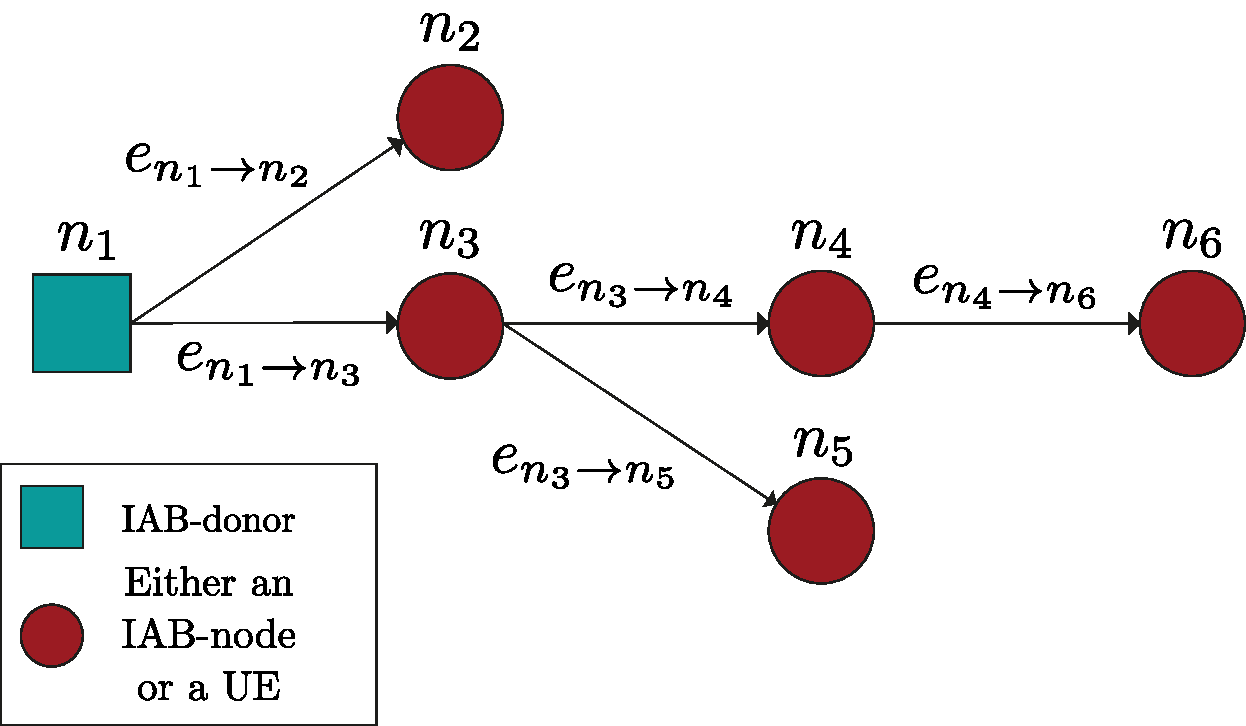
\includegraphics[width=0.7\linewidth]{Figures/CentralResourceManagement/IAB_Notation.pdf}}
    \caption{Comparison of the \gls{iab} network topologies analyzed in~\cite{3gpp_38_874} and related notation.}
    \label{Fig:IAB_top_not}
    % \vspace{-.6cm}  
\end{figure}

%TODO Explain scheduling and better formulation of the half-duplex explanation(e.g. the backhaul-aware)
Finally, the introduction of resource coordination mechanisms and related signaling is explicitly supported in the \gls{iab} specification drafts~\cite{3gpp_38_874, 3gpp_38_174}. Nevertheless, these solutions must reuse as much as possible the available NR specifications and
require at most minimal changes to the Rel.15 \gls{5gc} and \gls{nr}.

%According to these considerations, the remainder of this section will propose a generic algorithm for centralized access/backhaul resource partitioning which aims to be scalable, efficient and, in general, implementable in real-world deployments.

\subsection{System model}
\label{Subsec:sys_model}

According to these assumptions and referring to Fig.~\ref{Fig:IAB_notation}., a generic \gls{iab} network can be modeled as a directed graph $\mathcal{G} = \{\mathcal{N},  \mathcal{E} \}$, where the set of nodes $\mathcal{N} \mathop = \limits^{\Delta} \, \{ n_1, \, n_2, \, \ldots \, n_{\vert \mathcal{N} \vert }  \}$ comprises the \gls{iab}-donor, the various \gls{iab}-nodes and the \glspl{ue}. 
Accordingly, the set of directed edges $\mathcal{E} \mathop = \limits^{\Delta} \, \{ e_{1} , \, e_{2}, \, \ldots \, \allowbreak e_{\vert \mathcal{E} \vert} \} \equiv \{ e_{n_j \to n_k} \}_{j, k} $, where the edge $e_{n_j \to n_k}$ originates at the parent node $n_j$ and terminates at the children $n_k$, comprises in all the active cell attachments, either of mobile terminals to a \gls{gnb} or from \gls{iab}-nodes towards their parent node.
Since the goal of this paper is to study backhaul/access resource partitioning policies, this generic model can be actually simplified: in fact, all the \glspl{ue} connected to a given \gls{gnb} can be represented by a single node in $\mathcal{G}$ without any loss of generality. Similarly, the same holds true for their links toward the serving \gls{gnb}, which can then be represented by a single edge. 
%TODO Maybe mention that as a consequence the number of edges is significantly reduced, taking into consideration the expected # of UEs connected to a BS in 5G systems
Furthermore, this work focuses on \gls{st} topologies only. 

We define as \textit{feasible schedule} any set of links $\mathcal{E'} \subseteq \mathcal{E}$ such that none of them share a common vertex, i.e., $ \forall \, e_{n_j \to n_k} \neq e_{n_l \to n_m} \in \mathcal{E'}$ it holds that $n_{j} \neq n_{m}$ and $n_{l} \neq n_{k}$. Let then $f_u$ be a utility \textit{additive map}, namely, a function such that the overall utility experienced by the system when scheduling edges $e_1$ and $e_2$ satisfies $f_u (e_1, e_2) = f_u (e_1) + f_u(e_2)$. Let also $\mathcal{W} \mathop = \limits^{\Delta} \, \{ w_1, \, w_2, \, \ldots \, w_{\vert \mathcal{E} \vert } \}$ be the set of positive weights whose generic entry $w_j$ represents the utility which is obtained when scheduling the $j$-th edge, namely, $w_j \mathop = \limits^{\Delta} \, f_u (e_j)$. Then, the overall utility of the system is $\mathcal{U} \mathop = \limits^{\Delta} \, \sum_{e_k \, \in \, \mathcal{E'}} f_u(e_k) = \sum_{e_k \, \in \, \mathcal{E'}} w_k $.
The goal is to find the feasible set $\mathcal{E'}^{*}$ which maximizes the overall utility, i.e., $\underset{\mathcal{E'}}{\mathrm{argmax}} \,\, \mathcal{U} $. In computer science, this task is typically referred to as the \textit{Maximum Weighted Matching} problem~\cite{Korte2002}.

Finding the \gls{mwm} of a given graph, in the general case, is not trivial from a computational point of view. 
In fact, the fastest known \gls{mwm} algorithm for generic graphs has a complexity of \bigO{\vert V \vert \vert E \vert + \vert V \vert^2 \log{\vert V \vert}}~\cite{1990Gabow}, posing serious limitations to the suitability of such algorithm to \gls{5g} and beyond networks, which target a connection density of 1 million devices per km\textsuperscript{2}. However, we argue that under the aforementioned assumptions on the system model, which restrict the network to an \gls{st} topology, it is possible to design an \gls{mwm}-based semi-centralized resource partitioning framework which exhibits linear complexity with respect to the network size and which, as a result, is able to satisfy the scalability requirements highlighted by \gls{3gpp} in~\cite{3gpp_38_874}. 
Nevertheless, the proposed framework can be easily extended to the case of a \gls{dag} \gls{iab} network. In such regard, a sub-optimal strategy is to periodically discard, during each centralized allocation, the redundant edges of each node. In such a way, the input which is fed to the \texttt{T-MWM} algorithm is, effectively, an \gls{st}. A second, optimal extension can be obtained by computing at the controller the \gls{mwm} of the network via a generic \gls{mwm} algorithm, instead of using the \gls{st}-specific \texttt{T-MWM} as in the proposed framework. However, this strategy would feature a higher computational complexity.

\section{Semi-centralized resource allocation scheme for IAB networks}
\label{Sec:scheme_main}

This section presents an \gls{mwm} algorithm for \gls{st} topologies (Sec.~\ref{Sec:T-MWM}), an efficient and \gls{mwm}-based semi-centralized resource partitioning framework for \gls{iab} networks (Sec.~\ref{Sec:Cent-scheme}) and some considerations about its implementation (Sec.~\ref{Sec:ns3-impl}). 
Specifically, the proposed scheme collects at a controller installed on the \gls{iab}-donor L1 and/or L3 measurements from the various \glspl{gnb}. Then, it uses such information to build a weighted \gls{st} which represents the \gls{iab}-network. In particular, the network topology is inferred by examining the incoming parent-child associations. The edge weights are also computed from the received measurements, based on the specific policy (hence, of target \glspl{kpi}) of choice. Finally, the resource partitioning is optimized by computing an \gls{mwm} of the network and then prioritizing the links which comprise it. A high level diagram of is provided in Fig.~\ref{Fig:Diagram}.

\begin{figure}[t]
    \subfloat[IAB protocol stack and topology.\label{Fig:IAB-net}]{
    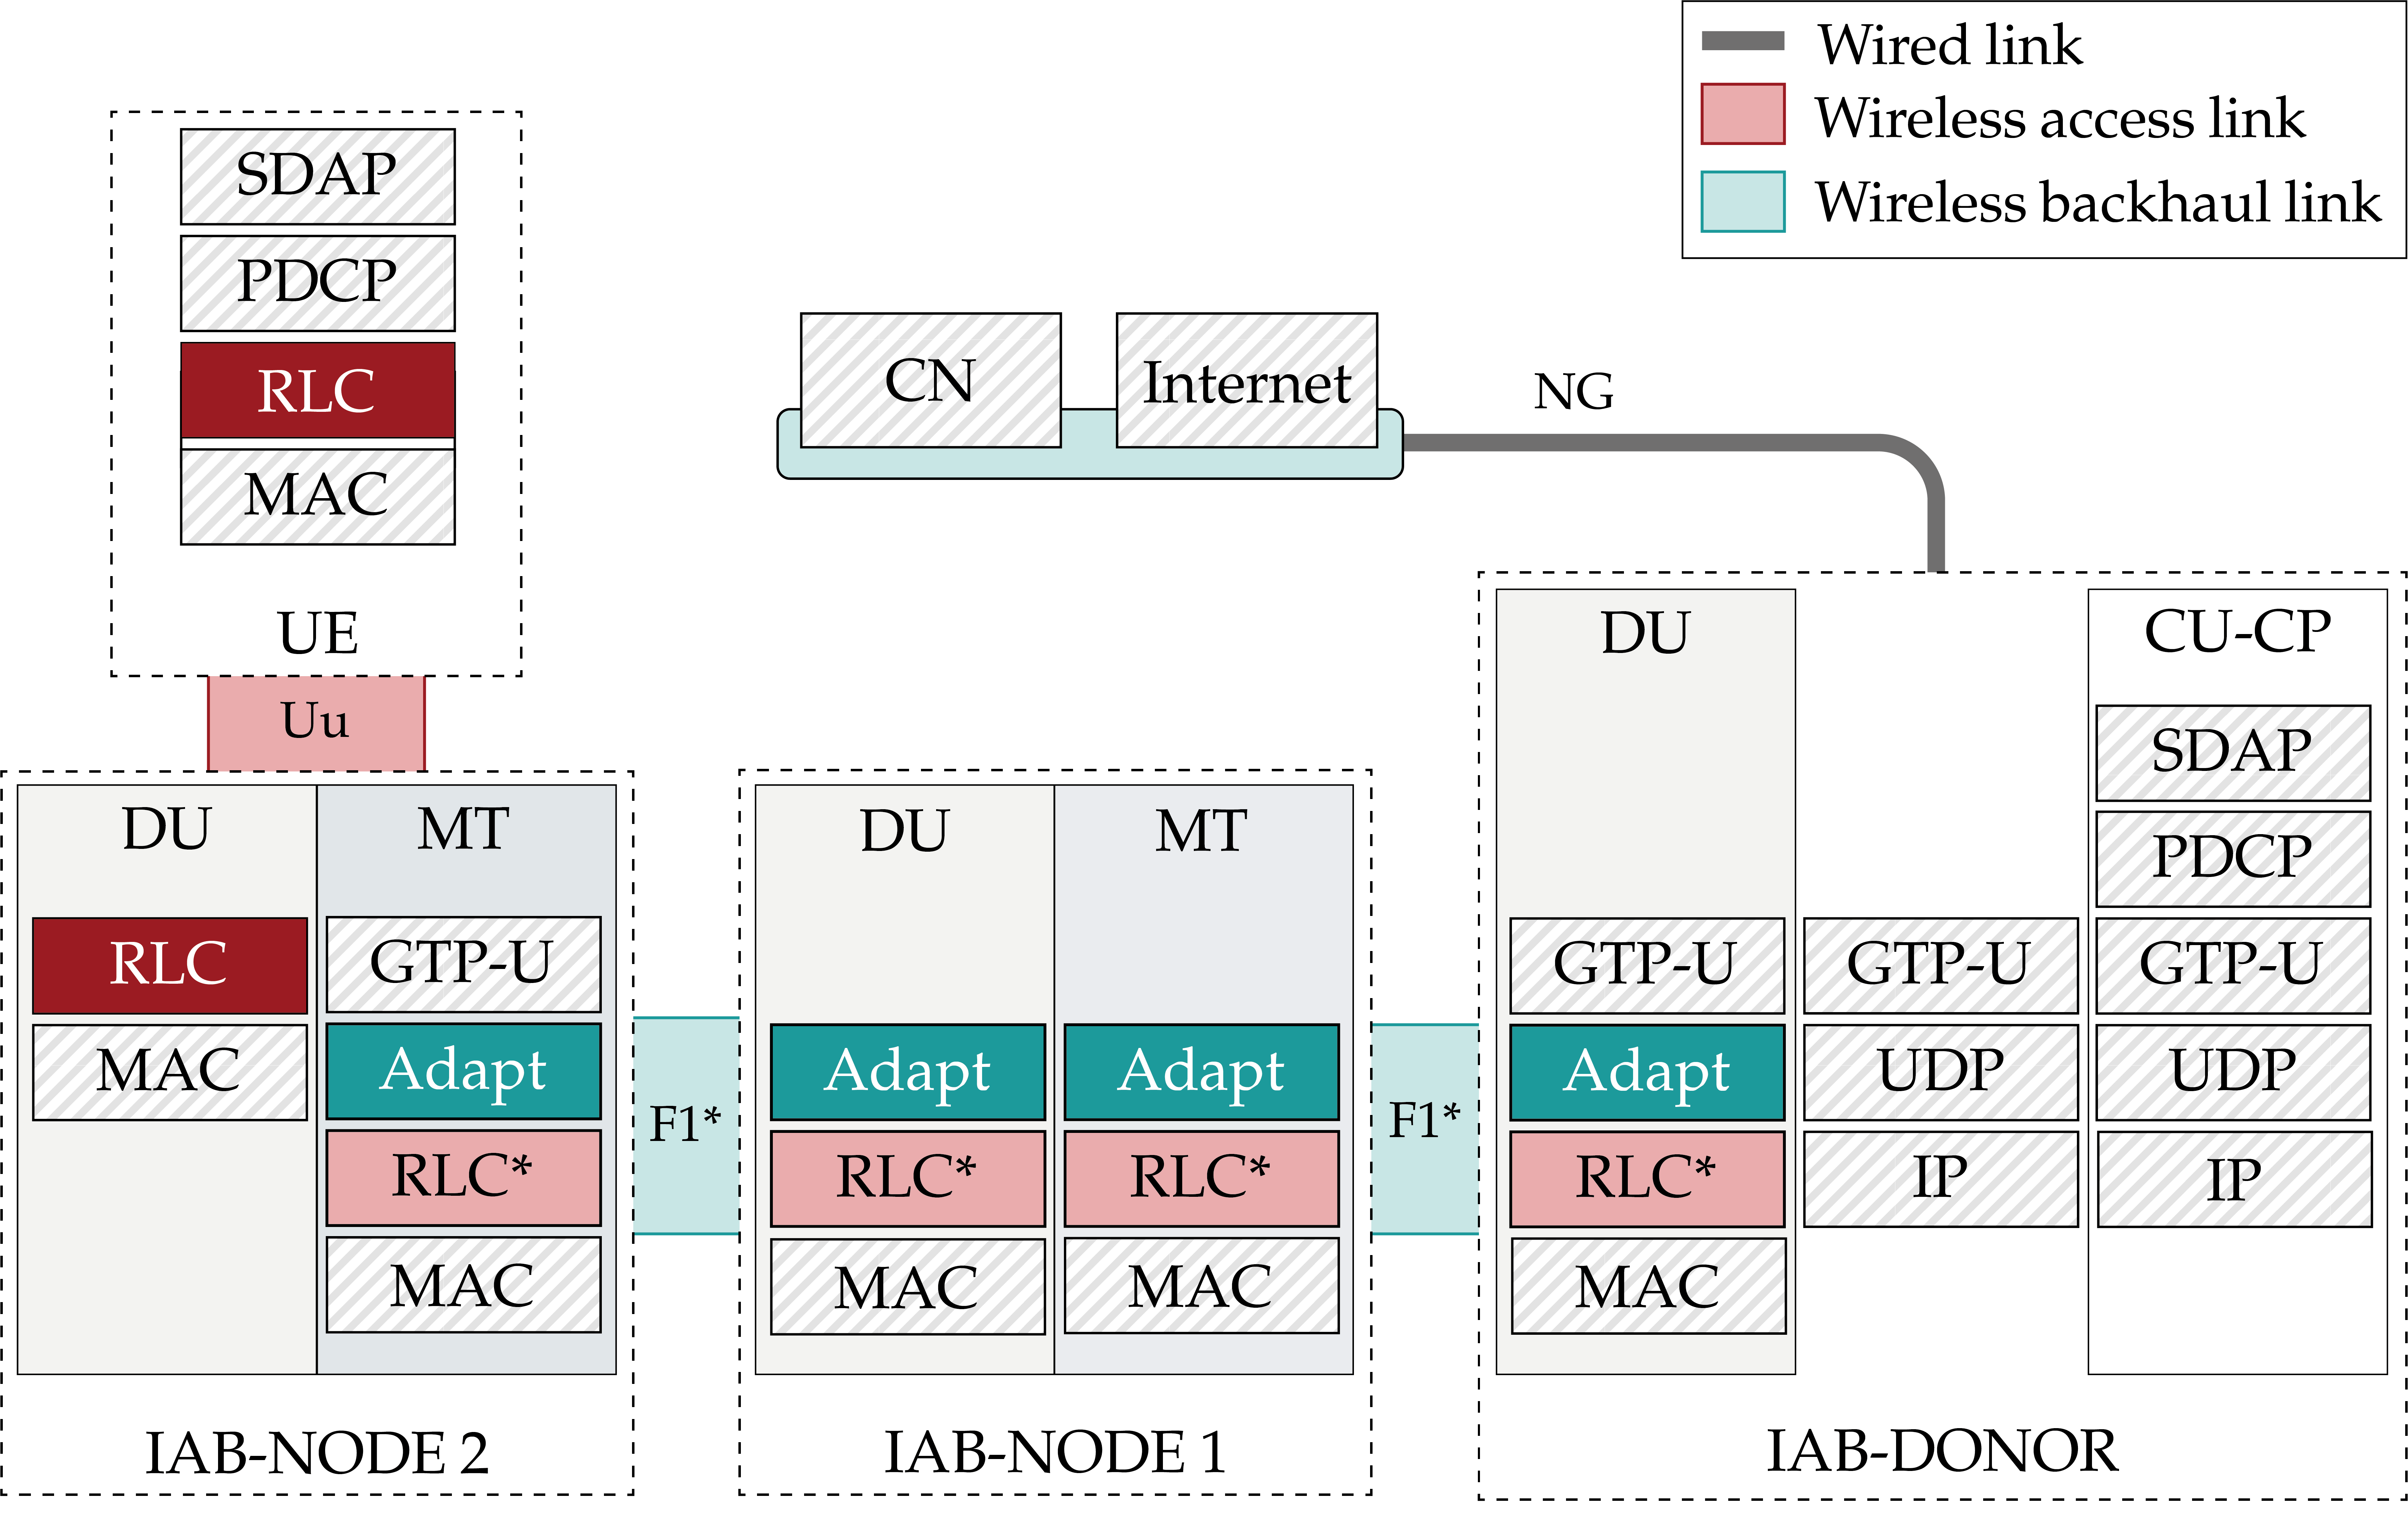
\includegraphics[width=0.95\linewidth]{Figures/CentralResourceManagement/architecture_full.png}}\hfill
    \subfloat[High level diagram of the proposed \gls{mwm}-based framework.\label{Fig:Diagram}]{
    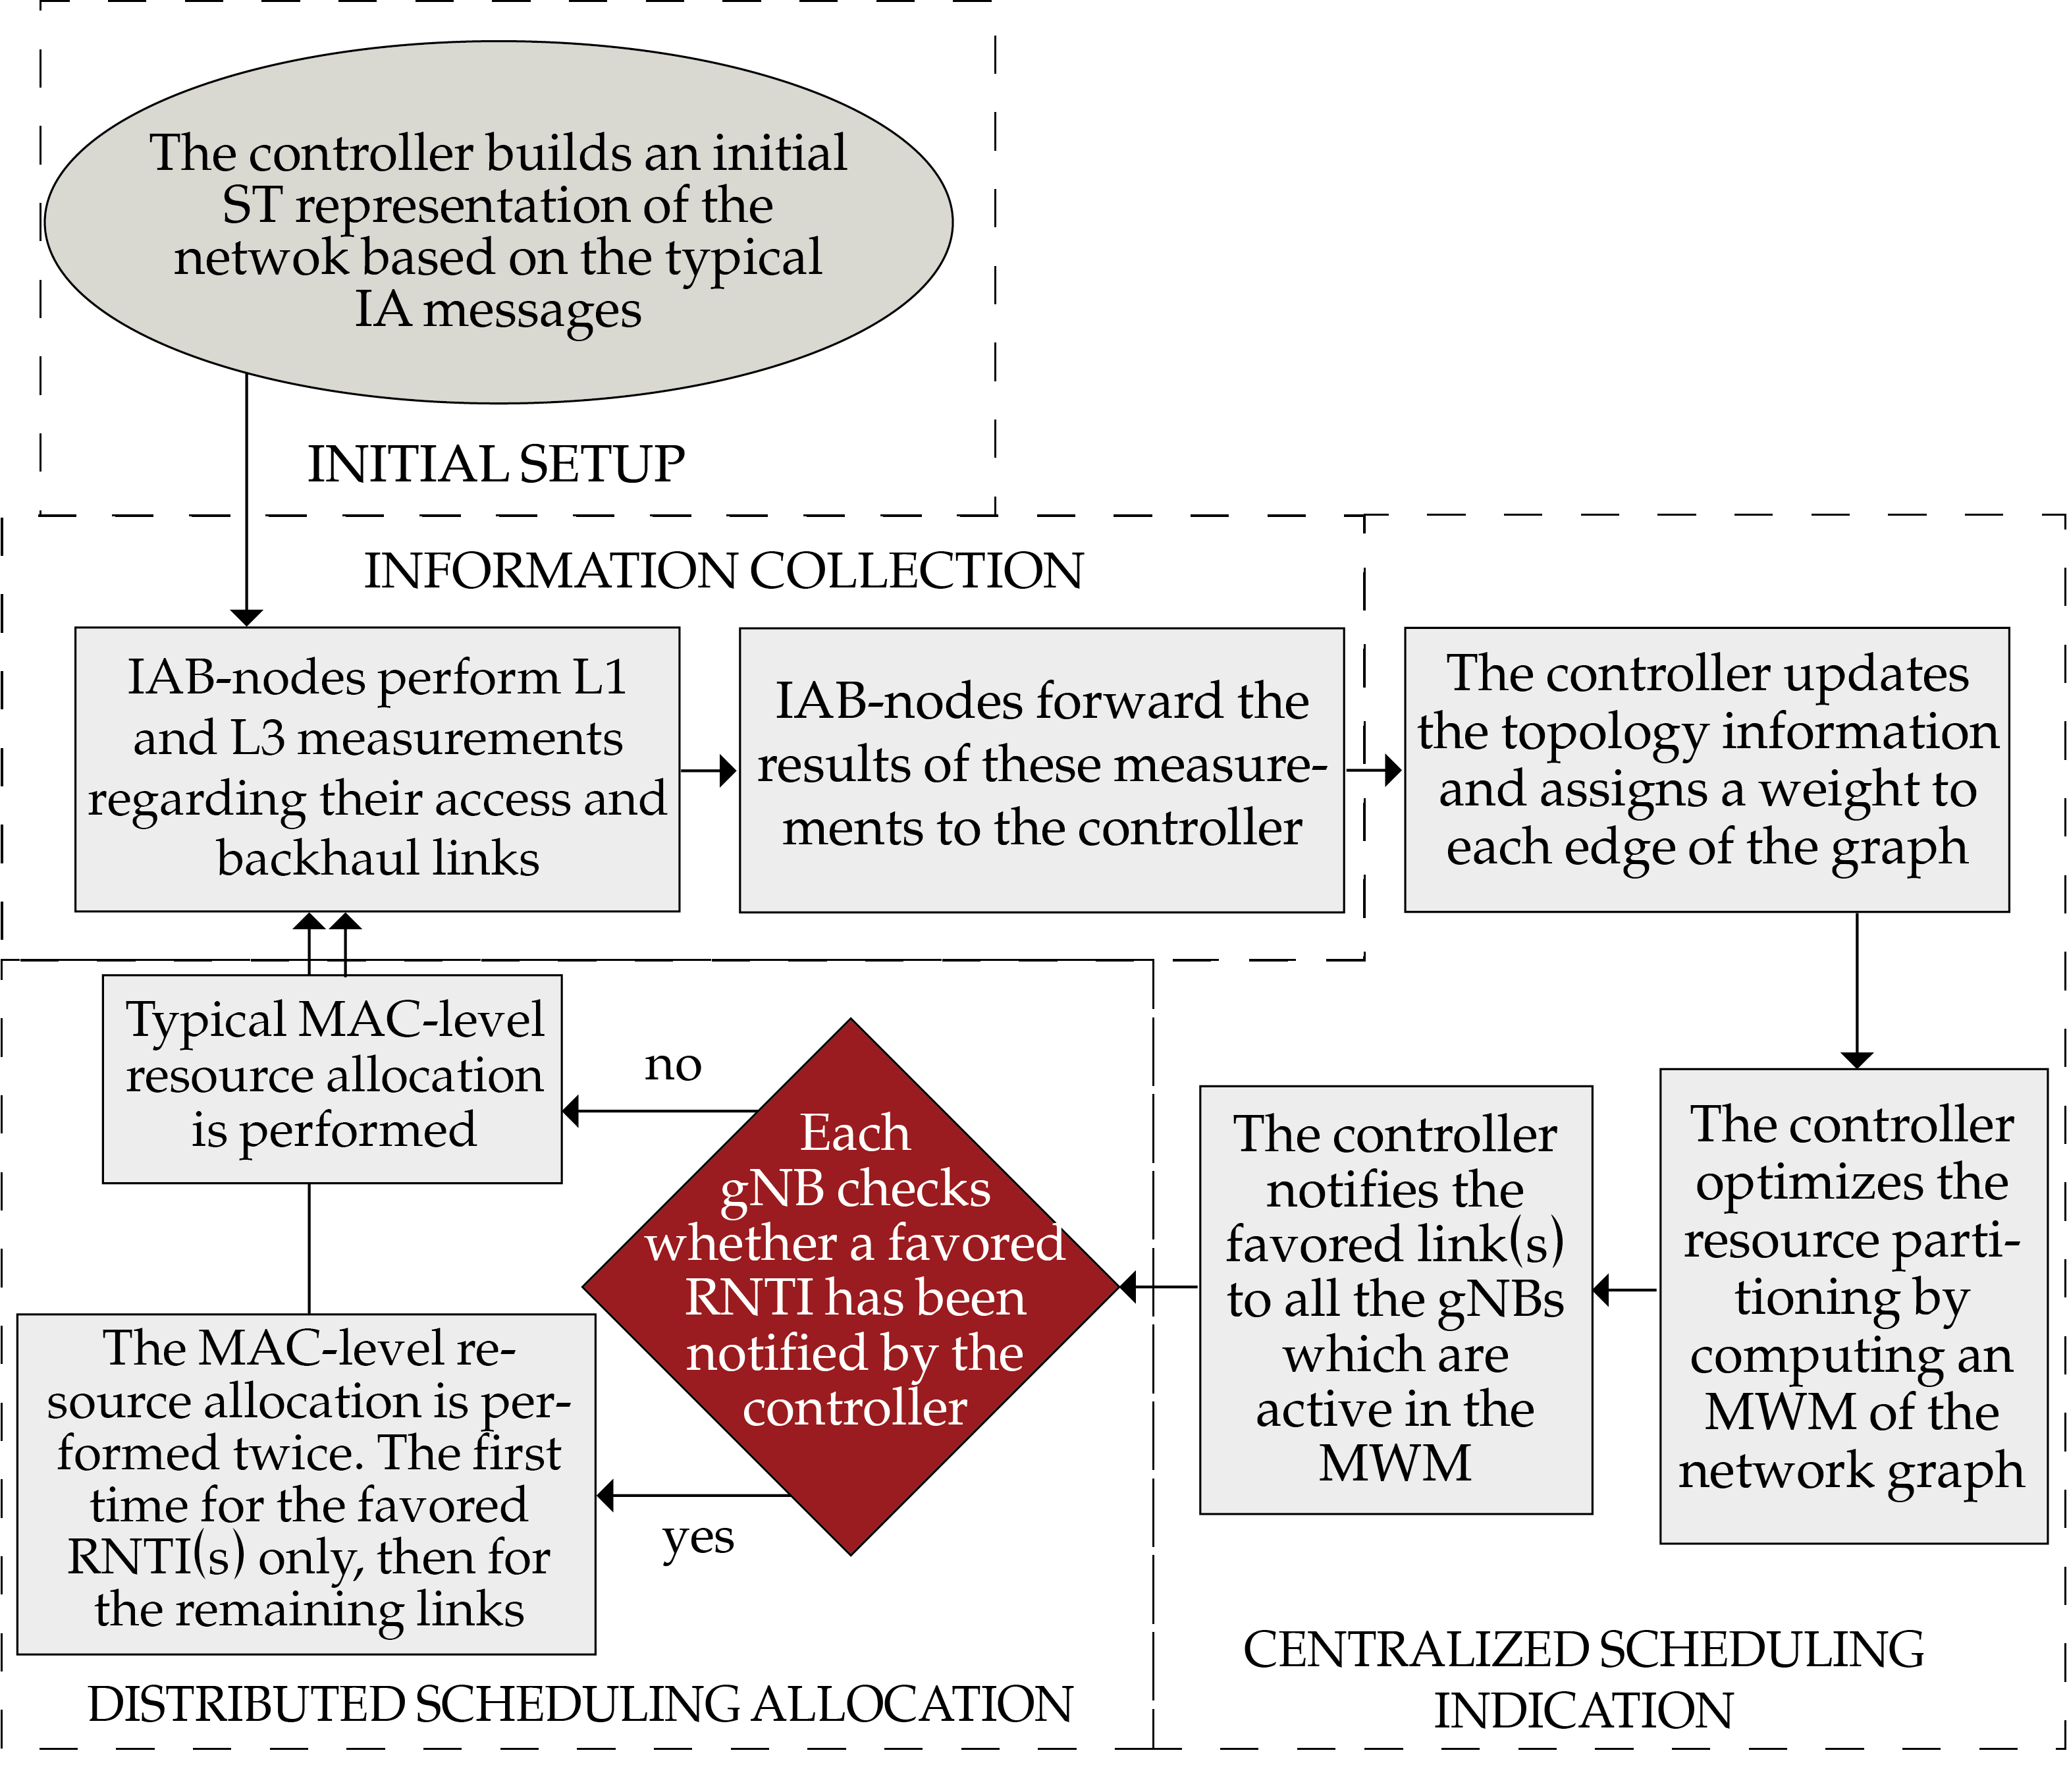
\includegraphics[width=0.95\linewidth]{Figures/CentralResourceManagement/FlowChart_IAB.png}}
    \caption{IAB topology and proposed MWM-based framework.}
    \label{fig:fr-top}
\end{figure}

\subsection{\gls{mwm} for \gls{st} graphs}
\label{Sec:T-MWM}

As the first of our contributions, we present an algorithm, hereby called \texttt{T-MWM}, which computes the \gls{mwm} of an \gls{st} in linear time. In particular, \texttt{T-MWM} is a bottom-up algorithm which, upon receiving as input a weighted \gls{st} $\mathcal{G}$ described by its edge map $\mathbf{E}$ and the corresponding weight map $\mathbf{W}$, produces as output a set of active edges $\mathbf{E^*}$ which are an \gls{mwm} of $\mathcal{G}$. That is to say, $\mathbf{E^*}$ is a matching of $\mathcal{G}$ which yields the globally maximum utility.
Furthermore, $\mathbf{E}$ is from now on assumed to exhibit the following invariant: each \gls{iab} parent precedes its children in the map, hence avoiding the need for a recursion. 
%TODO can remove this when we add the discussion on the complexity of each phase
This is automatically obtained as each \gls{iab} child connects after its parent, and is thus added to the map in a subsequent position.
Nevertheless, this assumption can be easily relaxed, albeit at the cost of losing as a side-effect the bottom-up design.

%TODO rewrite, do not include what used to be Lemma 1.
% Needs a link between these two sections

The proposed algorithm is designed starting from the observation that, given the generic node $n_k \in \mathcal{G}$ and a matching $\mathbf{\bar{E}}$ of $\mathcal{G}$, we can identify the following mutually exclusive and collectively exhaustive cases: $\mathbf{\bar{E}}$ can contain either one or zero edges which originate from $n_k$. Based on this fact, we then discern the optimal utilities which can be obtained in each of these cases. Specifically, we define the maximum utilities yielded by a matching of $n_k$'s sub-tree which either contains a link originating from $n_k$ or not as $\mathbf{F}(n_k)$ and $\mathbf{G}(n_k)$, respectively.
Then, as can be seen in Alg.~\ref{Alg:tmwm}, the \texttt{T-MWM} algorithm basically consists in two traversals of the network graph. During the first one we compute the $\mathbf{G}$ and $\mathbf{F}$ functions for all the nodes in $\mathcal{G}$ using the recursive formulas provided by Lemma~\ref{lemma_utils}. Finally, during the second traversal, this knowledge is used for computing an \gls{mwm} of the network; the correctness of this last phase is proved by Lemma~\ref{lemma_active_edges}.

%Specifically, these formulas are based on the following observations.
%First, given the generic internal node $n \in \mathcal{G}$, any \gls{mwm} contains an edge which originates either from $n$ or one of its children, as stated in Lemma~\ref{lemma_ch_par}. It follows that if the \gls{mwm} does not contain any edge which originates from $n$, the maximum utility is achieved when activating \textit{all} the edges which originate from its children. On the other hand, whenever the edge from $n$ to its generic child $m$ is included in the \gls{mwm}, the
%All together, these first two Lemmas prove the correctness of the first part of Alg.~\ref{Alg:tmwm}.

%TODO Maybe rework edges notation here as well, in order to make it slightly more uniform
\begin{algorithm}[tbp!]
\small
    \caption{Tree-Maximum Weighted Matching}
    \label{Alg:tmwm}
    \hspace*{\algorithmicindent} \textbf{Input:} A weighted \gls{st} $\mathcal{G}$ encoded by a map $\mathbf{E}$, which associates each node in $\mathcal{G}$ to its edges, and the corresponding weights map $\mathbf{W}$. \\ 
    \hspace*{\algorithmicindent} \textbf{Output:} An \gls{mwm} $\mathbf{E^*}$ of $\mathcal{G}$. 
    \begin{algorithmic}[1] % The number tells where the line numbering should start
        \Procedure{\texttt{T-MWM}}{$\mathbf{E}, \mathbf{W}$} 
            \State $\mathbf{F} \gets \mathbf{0}$; $\mathbf{G} \gets \mathbf{0}$ \Comment{Initialize the utility vectors to zero vectors}
            \State $\mathbf{E^*} \gets \{ \}$ \Comment{Initialize the set of active edges as empty}
            \For{each internal node $n_k \in \mathbf{E}$} \Comment{\parbox[t]{.43\linewidth}{In ascending order w.r.t. to their depth in $\mathcal{G}$}}
            \State $maxUtil \gets - \infty$;  $\mathbf{maxUtilChild}(n_k) \gets \{ \}$
            \For{each edge $e_{n_k \to n_j} \in \mathbf{E}(n_k) $} \Comment{Iterate over its edges}
                \State $\mathbf{G}(n_k) \gets \mathbf{G}(n_k) + \max \left\{ \mathbf{F}(n_j), \mathbf{G}(n_j) \right\}$
                \State $currUtil \gets \mathbf{W} ( e_{n_k \to n_j} ) - \left[ \mathbf{F}(n_j) - \mathbf{G}(n_j) \right]^+  $
            \If{$currUtil > maxUtil$}
            	\State $maxUtil \gets currUtil$;  $\mathbf{maxUtilChild}(n_k) \gets n_j$ 
            \EndIf
            \EndFor\label{edgesFor}
            \State $\mathbf{F}(n_k) \gets \mathbf{G}(n_k) + maxUtil$ 
            \EndFor\label{nodesFor}
			
			\For{each internal node $n_k \in \mathbf{E}$} \Comment{\parbox[t]{.43\linewidth}{In ascending order w.r.t. to their depth in $\mathcal{G}$}}			
			
				\If { $\mathbf{F}(n_k) \geq \mathbf{G}(n_k)$}
					\State $\mathbf{E^*} \gets \mathbf{E^*} \cup e_{n_k \to \mathbf{maxUtilChild}(n_k)}$
					\State $\mathbf{F}(\mathbf{maxUtilChild}(n_k)) \gets -\infty$ \Comment{\parbox[t]{.3\linewidth}{Ensure child does not get activated multiple times}}
				\EndIf\label{activeIf}
			\EndFor\label{edgesFor2}            
            
            \State \textbf{return} $\mathbf{E^*}$
        \EndProcedure
    \end{algorithmic}
\end{algorithm}

%\begin{lem}
%\label{lemma_ch_par}
%Let $n_k$ be an arbitrary internal node of $\mathcal{G}$ and $\{ n_j \}_k$ be the set of its children. Then, any \gls{mwm} of $\mathcal{G}$ must contain an edge which has as one of its vertices either $n_k$ or an element of  $\{ n_j \}_k$.
%\end{lem}
%
%\begin{IEEEproof}
%Suppose there exists an \gls{mwm} $\mathbf{E^*}$ of $\mathcal{G}$ which does not contain any such edge. Then the set $\hat{\mathbf{E}}^* \mathop = \limits^{\Delta} \, \mathbf{E^*} \cup \{ e_{n_k \to n_m} \}$, where $ e_{n_k \to n_m} $ is the edge from $n_j$ to its (arbitrary) child $n_m$ is still a feasible activation set, since no edge in $\mathbf{E^*}$ shares such vertices. Furthermore, since the weights are positive we have that $f_u (\hat{\mathbf{E}}^*) = f_u (\mathbf{E^*}) + \mathbf{W} (e_{n_k \to n_m}) > f_u (\mathbf{E^*}) $, which is clearly a contradiction.
%\end{IEEEproof}

\begin{lem}
\label{lemma_utils}
Given an \gls{st} $\mathcal{G}$, consider its generic internal node $n_k$. Let then $\mathbf{F}(n_k)$ be the maximum utility yielded by a matching of $n_k$'s sub-tree which activates a link originating from $n_k$, and $\mathbf{G}(n_k)$, conversely, the utility provided when such matching contains no links which feature $n_k$ as parent. Then, we have that:
\[ 
\begin{cases}
\mathbf{G}(n_k) = \sum\limits_{ \{ n_j \}_k} \max \left\{ \mathbf{F}(n_j), \mathbf{G}(n_j) \right\} \\

\begin{aligned}
\mathbf{F}(n_k) &= \mathbf{G}(n_k) + \underset{\{ n_j \}_k }{\max} \{ \mathbf{W} ( e_{n_k \to n_j} ) \\
&- \left[ \mathbf{F}(n_j) - \mathbf{G}(n_j) \right]^+ \}
\end{aligned}


\end{cases}
\]
where the set $\{ n_j \}_k$ comprises all the children of $n_k$ and $\left[ x \right]^+ = \max\{x, 0\}$ is the positive part of $x$.
%
Conversely, for leaf nodes $n_l$ it holds that $\mathbf{F}(n_l) \equiv \mathbf{G}(n_l) \equiv 0 $.
\end{lem}

\begin{proof}
This lemma can be proved by induction over the height $h_k$ of the sub-tree corresponding to node $n_k$. The base case is $h_k = 0$, i.e., when $n_k$ is a leaf node; in this case, trivially, both $\mathbf{F}(n_k)$ and $\mathbf{G}(n_k)$ are zero since no links exhibit $n_k$ as parent node and the sub-tree of $\mathcal{G}$ which originates in $n_k$ consists of $n_k$ only, respectively.

Then, assume that $n_k$'s sub-tree exhibits a generic height $h_k > 0$, and that the above formulas hold for each of its children sub-trees, which exhibit a height $h_j < h_k$. If we do not activate any edge which originates from $n_k$, then no added constraints are introduced concerning the edges which can be activated in its children sub-trees. Therefore, %the maximum utility achieved by any matching of $n_k$'s sub-tree, without activating any node which originates from $n_k$, 
$\mathbf{G}(n_k)$ is simply the sum of the utilities achieved by any \gls{mwm} computed on its children sub-trees, i.e.,  $\mathbf{G}(n_k) = \sum\limits_{ \{ n_j \}_k} \max \left\{ \mathbf{F}(n_j), \mathbf{G}(n_j) \right\}$.
The remaining option is to activate exactly one edge, hereby called $e_{n_k \to n_m}$, which originates from $n_k$. In this case, no additional edges which feature $n_m$ as parent can be added to the matching. As a consequence, the contribution of $n_m$'s sub-tree on $\mathbf{F}(n_k)$ reads $\mathbf{G}(n_m)$. Conversely, no additional constraints are introduced regarding the other nodes. It follows that the utility obtained in this instance reads:
\[ \sum_{ \{ n_j \neq n_m\}_k } \max \left\{ \mathbf{F}(n_j), \mathbf{G}(n_j) \right\} +  \mathbf{W} ( e_{n_k \to n_m} ) + \mathbf{G}(n_m) \]
and can be rewritten as:
\[  \mathbf{G}(n_k) + \mathbf{W} ( e_{n_k \to n_m} ) - \left[ \mathbf{F}(n_m) - \mathbf{G}(n_m) \right]^+ \]
Finally, such utility is clearly maximized when $n_m$ is chosen as $ \underset{ \{ n_j \}_k }{\mathrm{argmax}} \, \{ \mathbf{W} ( e_{n_k \to n_j} ) - \left[ \mathbf{F}(n_j) - \mathbf{G}(n_j) \right]^+ \}$, yielding:
\[ \mathbf{F}(n_k) = \mathbf{G}(n_k) + \underset{\{ n_j \}_k }{\max} \, \{ \mathbf{W} ( e_{n_k \to n_j} ) - \left[ \mathbf{F}(n_j) -  \mathbf{G}(n_j) \right]^+ \} \qedhere \] 
\end{proof}

\begin{lem}
\label{lemma_active_edges}
Given an \gls{st} $\mathcal{G}$ of root $n_r$ and the $\mathbf{F}$ and $\mathbf{G}$ functions computed as per Lemma~\ref{lemma_utils}, an \gls{mwm} $\mathbf{E^*}$ of $\mathcal{G}$ can be computed by performing the following procedure:
%, in a recursive fashion
\begin{enumerate}
\item If $ \, \mathbf{F}(n_r) \geq \mathbf{G}(n_r) $, add to $\mathbf{E^*}$ the edge from $n_r$ to $n_m$, where the latter is defined as $n_m \mathop = \limits^{\Delta} \, \underset{ \{ n_j \}_r }{\mathrm{argmax}} \, \{ \mathbf{W} ( e_{n_r \to n_j} ) - \left[ \mathbf{F}(n_j) - \mathbf{G}(n_j) \right]^+ \}$. Then, repeat recursively on all the sub-trees corresponding to $n_r$'s children $\{ n_j\}_r \, \vert \, n_j \neq n_m$ and on the children of $n_m$ itself.
\item If $ \, \mathbf{F}(n_r) < \mathbf{G}(n_r) $, repeat recursively on all the sub-trees corresponding to $n_r$'s children.
\end{enumerate}
\end{lem}

%TODO Add more details
\begin{proof}
The above procedure always yields a feasible activation, i.e., a matching of $\mathcal{G}$.  In particular, in either options we never recurse on a node which has already been activated, hence no pair of edges $\in \mathbf{E^*}$ can share any vertices. Furthermore, due to the properties of $\mathbf{F}$ and $\mathbf{G}$, whenever $\mathbf{F}(n_r) \geq \mathbf{G}(n_r)$ a matching yielding maximal utility can be obtained by activating the edge $e_{ n_r \to n_m }$, where $n_m \mathop = \limits^{\Delta} \, \underset{ \{ n_j \}_r }{\mathrm{argmax}} \, \{ \mathbf{W} ( e_{n_r \to n_j} ) - \left[ \mathbf{F}(n_j) - \mathbf{G}(n_j) \right]^+ \}$.
Since the procedure is then recursively repeated on $n_r$'s children and the validity of $\mathbf{F}$ and $\mathbf{G}$ properties holds for each sub-tree in $\mathcal{G}$, the set of edges $\mathbf{E^*}$ produced by the above procedure comprise a \textit{maximal} matching, i.e., they yield the maximum possible utility among all the feasible schedules. 
\end{proof}

%TODO consider moving this paragraph to the framework steps, together with the complexity and overhead considerations provided in the review for all the framework steps
Regarding the computational complexity of the proposed algorithm, it can be observed that during the first phase the main loop effectively scans each edge of $\mathcal{G}$, hence exhibiting a complexity \bigO{\vert \mathbf{E} \vert}. Moreover,
the second phase of \texttt{T-MWM} has complexity \bigO{\vert \mathbf{V} \vert}, since it loops through all the network nodes.
Therefore, we can conclude that the overall asymptotic complexity of the algorithm is \bigO{\vert \mathbf{V} \vert + \vert \mathbf{E} \vert}, or, equivalently, \bigO{\vert \mathbf{V} \vert} since in an \gls{st} the number of edges equals $\vert \mathbf{V} \vert - 1$.

\subsection{Semi-centralized resource partitioning scheme}
\label{Sec:Cent-scheme}
Based on the system model introduced in Sec.~\ref{Sec:Sys-model}, and the \texttt{T-MWM} algorithm, we present a generic optimization framework which partially centralizes the backhaul/access resource partitioning process, in compliance with the guidelines of~\cite{3gpp_38_874}. 
The goal of this framework is to aid the distributed schedulers, adapting the number of \gls{ofdm} symbols allocated to the backhaul and access interfaces to the phenomena which exhibit a sufficiently slow evolution over time, i.e., large scale fading and local congestion. % Maybe mention also effectiveness of centralized is exarcebated by TDD constraints
This optimization is undertaken with respect to a generic additive utility function $f_u$. An \gls{iab} network of arbitrary size is considered, composed of a single \gls{iab}-donor, multiple \gls{iab}-nodes and a (possibly time-varying) number of \glspl{ue} which connect to both types of \glspl{gnb}. %TODO Ask Tommaso/Michele 
%The choice of neglecting cooperation among neighboring sectors is motivated by the fact that different \gls{iab}-donors are likely to be separated by a distance which is significantly greater than their respective coverage area (in fact, if this would not be the case, there would not be the need for \gls{iab} in the first place). % Not impossible, but arguably sub-optimal
%Therefore, we deem an inter \gls{iab}-donors resource coordination to be an unrealistic scenario, which as a consequence is out of the scope of this paper.
%TODO But wired info exchange is actually possible (X2), needs further work or remove entirely 
Furthermore, %let the topology of the \gls{iab} network be pre-computed, for instance by using the policies of~\cite{polese2018iab}, and 
assume that a central controller is installed on the \gls{iab}-donor. 

The proposed framework can be subdivided into the following phases, which are periodically repeated every $T_{alloc}$ subframes:
\begin{enumerate}
\item \label{Enum_frameword:item_one} \textbf{Initial setup}. This step, which is depicted in Fig.~\ref{Fig:Phase0}, consists in the computation of the simplified \gls{iab} network graph $\mathcal{G} \equiv \{ \mathcal{V}, \mathcal{E} \}$. Specifically, after this phase $\mathcal{V}$ comprises the donor and the various \gls{iab}-nodes. Accordingly, $\mathcal{E}$ contains their active cell associations.

\item \label{Enum_frameword:item_two} \textbf{Information collection}. During this phase, the various \gls{iab}-nodes send to the central controller a pre-established set of information for each of their children in $\mathcal{G}$. For instance, this feedback may consist in their congestion status and/or  information regarding their channel quality. To such end, the implementation of this paper uses modified versions of pre-existing \gls{nr} Release 16 \glspl{ce}, as strongly recommended in the \gls{iab} SI~\cite{3gpp_38_874}. However, the scheme does not actually impose any limitations in such regard.
\item \label{Enum_frameword:item_three} \textbf{Centralized scheduling indication}. Upon reception of the feedback information, the central controller updates $\mathcal{G}$ by inspecting the received node-parent associations. Then, the set of weights $\mathcal{W}$ is calculated and an \gls{mwm} of $\mathcal{G}$ is computed, using the \texttt{T-MWM} algorithm. The output of this procedure is the activation set $\mathbf{E^*}$, which yields a globally optimum solution with respect to the chosen utility function. Subsequently, $\mathbf{E^*}$ is used as to create a set of \textit{favored} downstream nodes, i.e., of children which will be served with the highest priority by their parent, as depicted in Fig.~\ref{Fig:Phase2}. Finally, these scheduling indications are forwarded to the various \gls{iab}-nodes which act as parents in the edges of $\mathbf{E^*}$.

\begin{figure}[tbp]
	\centering
	%\captionsetup{singlelinecheck=false, justification=justified}
  % this sets the width of the figure, adjust to your needs
  	\subfloat[The original topology, exhibiting the actual cell attachments, is depicted on the left. Conversely, the reduced one is shown on the right.\label{Fig:Phase0}]{
  	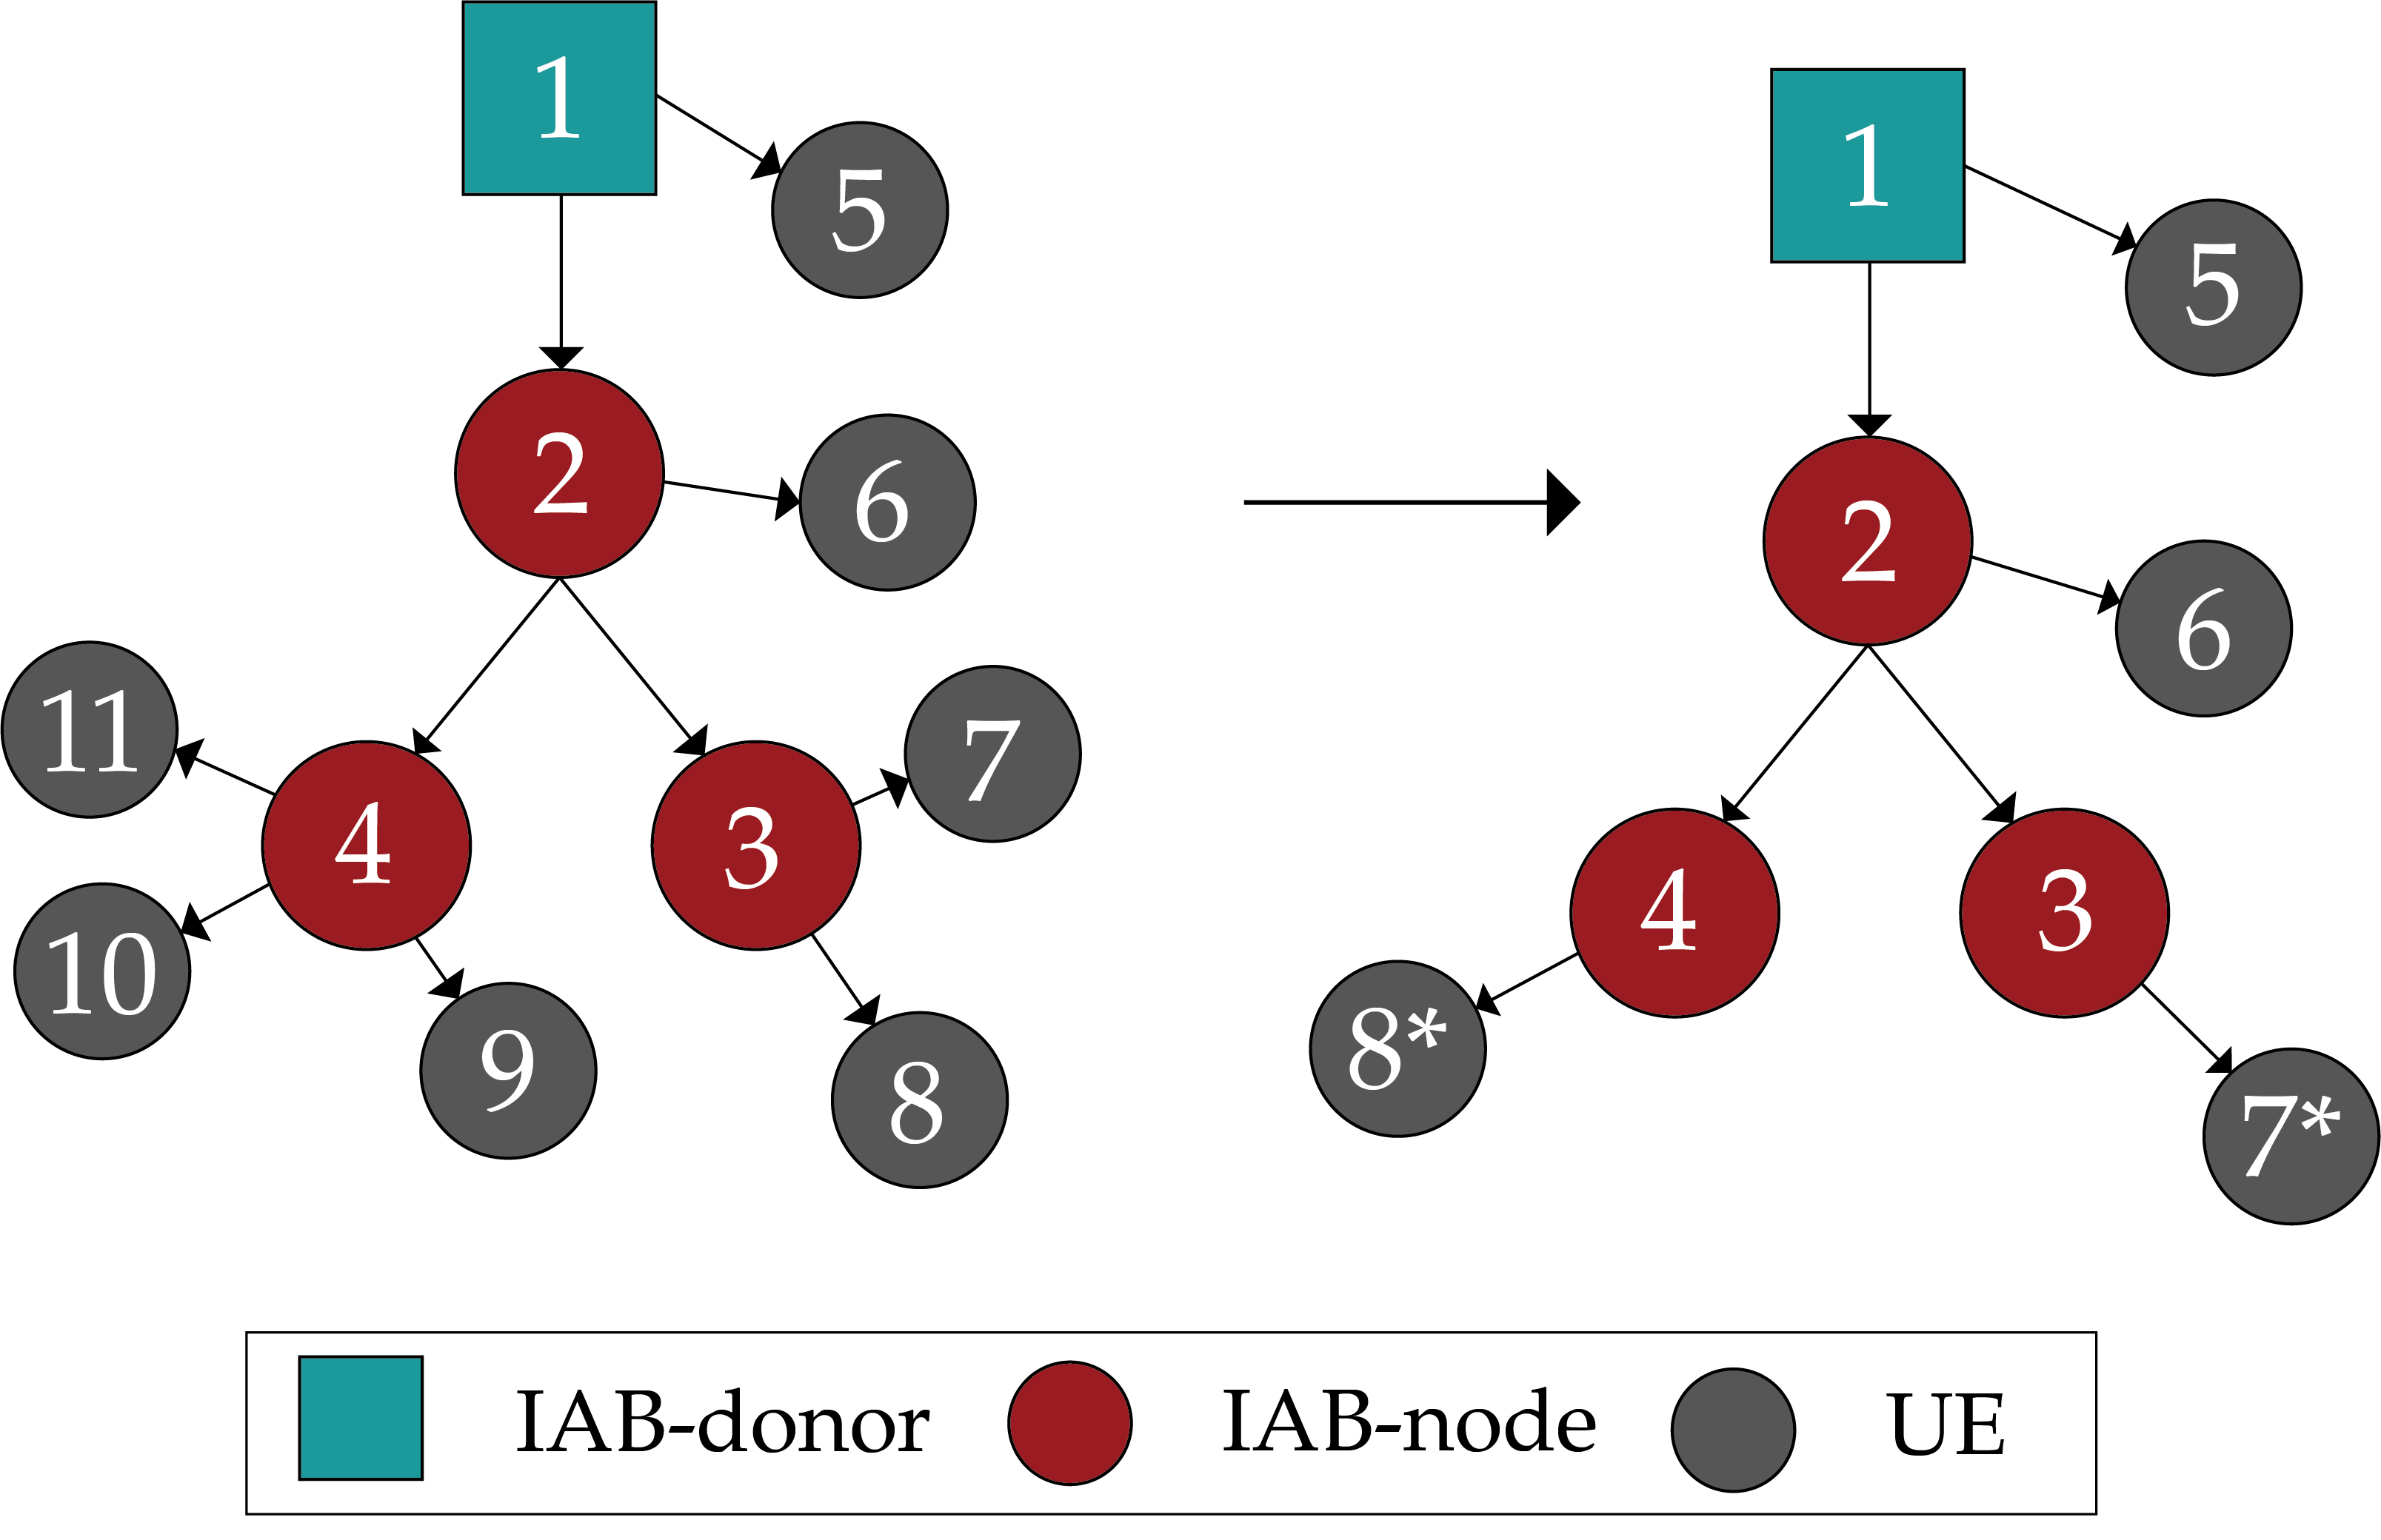
\includegraphics[width=0.7\linewidth]{Figures/CentralResourceManagement/Phase0.png}
    }\hfill
  	\subfloat[Computation of the \gls{mwm} and of the corresponding scheduling indications.\label{Fig:Phase2}]{
  	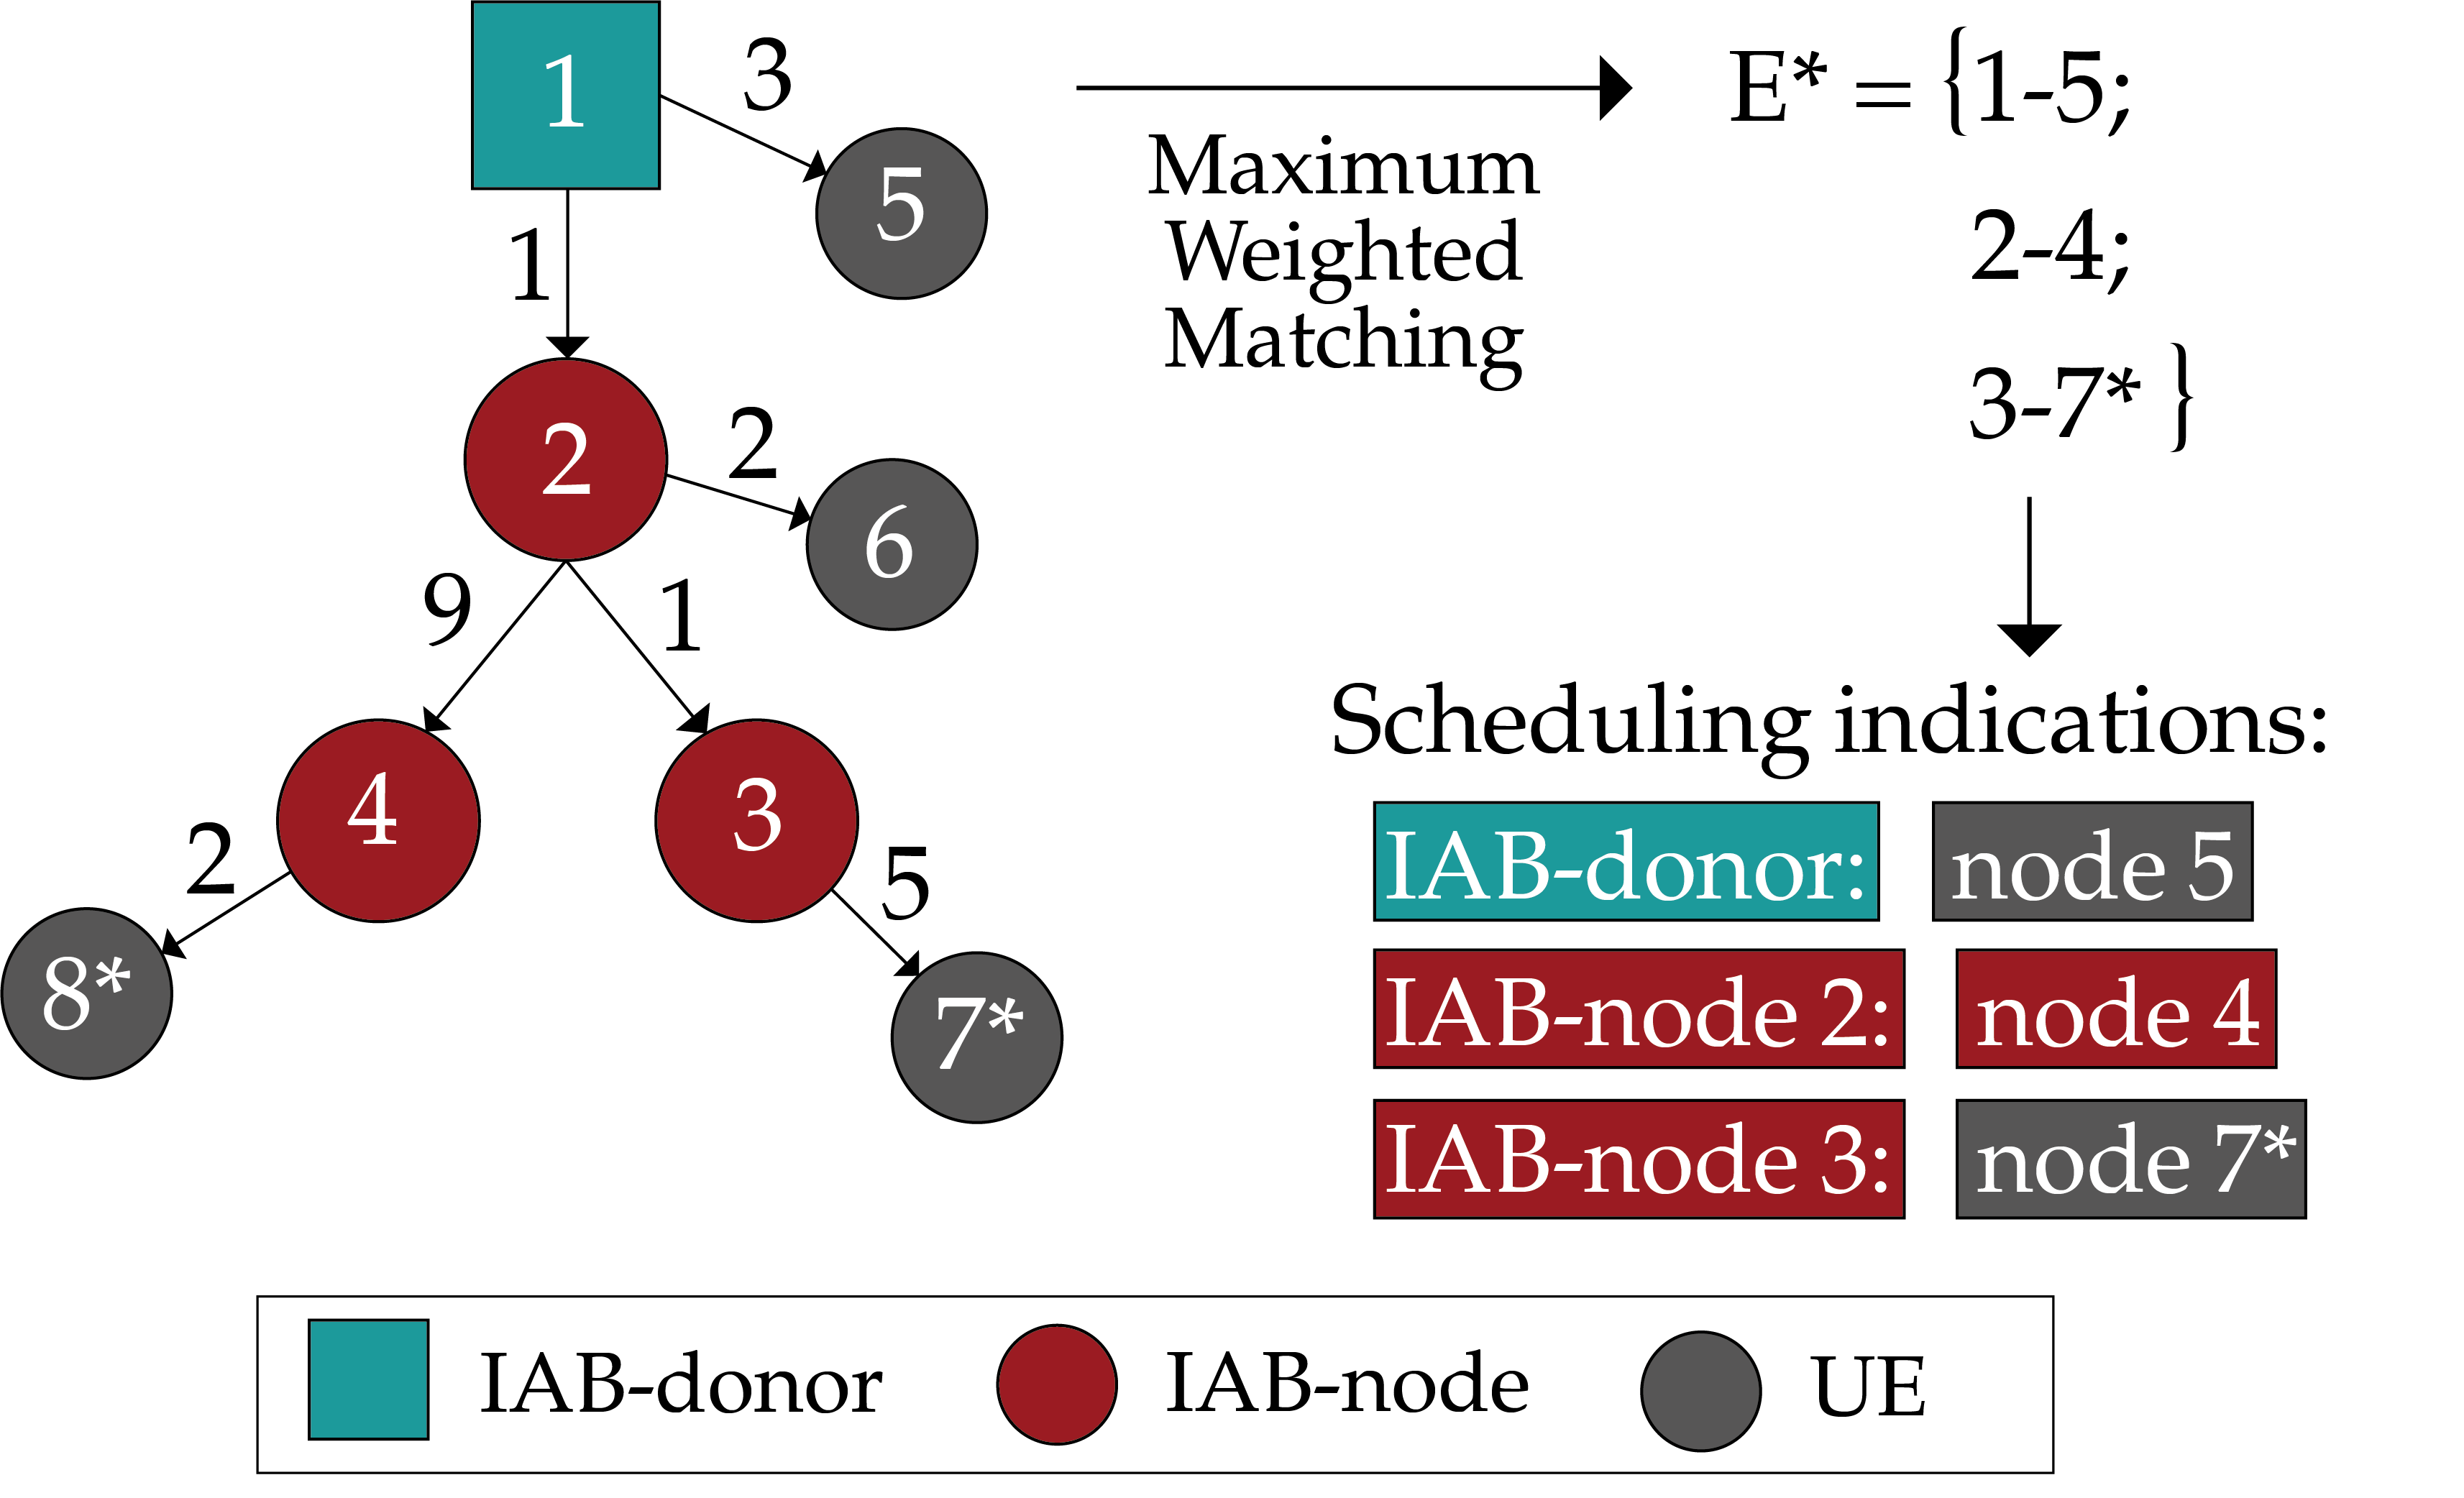
\includegraphics[width=0.7\linewidth]{Figures/CentralResourceManagement/Phase2.png}
    }
    \caption{High level scheme of the initial setup and centralized scheduling indication phases.}
    \label{Fig:Phases}
    %\vspace{-.6cm}  
\end{figure}


\item \textbf{Distributed scheduling allocation}. During this phase, the various \gls{iab}-nodes make use of the indications received by the central controller, if available, in order to perform the actual scheduling (which is, therefore, predominantly distributed). Specifically, the favored nodes are served with the highest priority, while the remaining downstream nodes are scheduled if and only if the resource allocation of the former does not exhaust the available \gls{ofdm} symbols.
\end{enumerate}
It is important to note that since $\mathcal{G}$ contains only the \gls{iab}-nodes, the donor and at most one ``representative" \gls{ue} per \gls{gnb}, the proposed scheme effectively performs only the backhaul/access resource partitioning in a centralized manner. On the other hand, the actual \gls{mac}-level scheduling is still undertaken in a distributed fashion, albeit leveraging the indications produced by the central controller. The major advantages which this two-tier design exhibits, compared to a completely centralized solution, are the presence of a relatively light signaling overhead and the ability to promptly react to fast channel variations, for instance caused by small scale fading.  

\subsection{Implementation of semi-centralized allocation schemes in mmWave \gls{iab} networks}
\label{Sec:ns3-impl}

The remainder of this section discusses how the proposed scheme can be implemented in \gls{iab} deployments, with references to how the \gls{3gpp} specifications can support it. Moreover, an in-depth analysis of the framework's communication overhead and computational complexity is provided. To such end, let $\mathcal{G} = \{ V, E \}$ be the reduced network graph, computed as per Sec.~II-C, and, conversely, let $\mathcal{\bar{G}} = \{ \bar{V}, \bar{E} \}$ comprise all the nodes in the \gls{iab} network.
% presents an implementation of the proposed scheme in the network simulator ns-3, along with considerations on its implementation in real world deployments.

In general, the resource allocation framework requires (i) a central controller, which is installed on the \gls{iab}-donor, or could be deployed in a \gls{ric} following the O-RAN architecture~\cite{bonati2020open}; and (ii) a scheduler which exchanges resource coordination information with the former. %and computes the weights for the resource allocation.
In particular, and referring to the aforementioned phases of the proposed scheme, the following %communication overhead, computational complexity and implementation  
additional considerations can be made. 

% Might be of interest and/or relevant
% In particular, \gls{rlc} bearers are independently setup for each hop in the \gls{iab}-network and an above-\gls{pdcp} adaptation layer forwards the various packet to either the access or the backhaul \gls{pdcp}s. Therefore, \textit{MmWaveIabNetDevice}s exhibit all the L2 \gls{5g} stack layers up to and including the latter, as can be seen in Fig.~\ref{Fig:mmWaveIabNetDevice}.

\subsubsection{Initial setup}
%The setup of the various centralized mechanisms is subdivided into two sub-phases: an initial configuration, where the relevant entities are initialized, and a periodic update of the topology information.
%The initial configuration . 
During this phase, which takes place when the \gls{iab}-nodes perform their first connection to the network, the controller acquires preliminary topology information by leveraging the configuration messages which are already exchanged during the typical Rel.16 \gls{ia} procedure~\cite[Sec. 9.6]{3gpp_38_874}. Therefore, no additional overhead is introduced. 
Specifically, a map which associates each \gls{iab}-node in the network to a list of its edges, identified by global identifiers (which from now on will be referred to as ``IDs"), is computed. %Since this phase takes place when no \gls{ue} has performed its \gls{ia} procedure yet, the exchanged topology information concerns the donor and \gls{iab}-nodes only.
As a consequence, $\mathcal{O} \left( \vert V \vert \right) $ insertions in a sorted map are performed and this one-time setup exhibits a computational complexity of $\mathcal{O} \left( \vert V \vert \log( \vert V \vert ) \right) $.

\subsubsection{Information collection}
The generation of the feedback information is performed in a distributed manner by  the \glspl{gnb}. To such end, the current implementation features the forwarding of information on the channel quality and buffer status, in the form of \glspl{cqi} and \glspl{bsr} respectively. This choice is driven by both the will of maximizing the re-utilization of the \gls{nr} Rel.16 specifications and the goal of making use of \gls{mac}-level \glspl{ce} only, hence avoiding the introduction of any constraint regarding the supported \gls{iab}-relaying architecture.
% Not so relevant for real deployments
%This periodic feedback to the controller is started by the \texttt{Do\-Sched\-Trigger\-Req} method of the various \texttt{MmWave\-RrIab\-Mac\-Scheduler} instances, which in turn calls the \texttt{Gen\-Cumulative\-Map} methods each subframe. However, the central controller can periodically discard the received feedback; by leveraging this possibility, the information collection can be configured to exhibit a period of $T_{collect} > 1$ subframes. 
In particular, the \gls{cqi} and \gls{bsr} information is generated by analyzing the corresponding \glspl{ce}, which are already received by the scheduler of each \gls{gnb}, and checking whether the source \gls{rnti} belongs to an \gls{iab}-node or to a \gls{ue}. In the first case, the corresponding ID
%\footnote{This change of identifiers is extremely important, as \gls{rnti}s are unique only within the scope of the \gls{gnb} they are attached to. Conversely, the IDs are globally unambiguous by design, hence suited for identifying terminals which may be connected to different \gls{gnb}s. \textbf{TODO: is this footnote necessary?}} 
is retrieved and an entry carrying such identifier along with its \gls{cqi}/\gls{bsr} value is generated. 
The feedback information concerning the \glspl{ue}, instead, is averaged in the case of the \glspl{cqi} and added up for the \glspl{bsr}, to obtain a single value for each \glspl{gnb}.
%It can be noted that both \glspl{cqi} and \glspl{bsr} are available to the scheduler, since the UL buffer statuses are already periodically reported by the downstream nodes via their \gls{bsr}s and the DL statuses can be easily retrieved by the former, since the \gls{rlc} buffers reside on the same node as the scheduler itself, i.e., the \gls{gnb}.

Referring to the \gls{3gpp} specifications of~\cite{3gpp_38_321}, the buffers occupancy can then be forwarded to the \gls{iab}-donor by introducing a Short \gls{bsr}, which carries a single \gls{lcg} ID and its respective buffer size. This is motivated by the fact that we do not keep track of per-flow information, i.e., we aggregate all the different \gls{rlc} bearers into a single measurement report. 
Similarly, the channel qualities can be reported by the various \gls{iab}-nodes via an additional \gls{cqi}-only \gls{csi} report, based on a \gls{wb} measurement. Therefore, we can upper bound the size of these \glspl{ce} as 11~\cite{3gpp_38_321} and 7 bits~\cite{3gpp_r1_1713763} respectively. 
%Both additional \glspl{ce} leverage pre-existing \gls{nr} measurements: the main novelty would be the introduction of their periodic reporting to the \gls{iab}-donor. 
%To such end, the \gls{5g} \gls{cqi} and \gls{bsr} data-structures require an additional field which carries the ID, if the chosen \gls{iab}-relaying architecture does not feature an Adaptation Layer~\cite{3gpp_38_874}. Conversely, relaying solutions which support the latter can reuse the \gls{nr} \glspl{ce} and let such layer introduce an additional header.
Regarding the computational complexity, in this phase we generate, at each \gls{gnb}, one \gls{cqi} and one \gls{bsr} for each backhaul link, and (possibly) compute one cumulative \gls{cqi} and \gls{bsr} for the \glspl{ue}. Therefore, the asymptotic complexity of this phase can be identified as $ \mathcal{O} \left(\vert V \vert \right)$.

\subsubsection{Centralized scheduling indication}
\label{Sec:cent_indic}
During this phase, the controller makes use of the feedback received from the \glspl{gnb} to update the topology information, compute the weights of the various network links and to generate the centralized scheduling indications. 

Regarding the former, no additional control information is required. In fact, the periodic feedback received from the various \gls{iab}-nodes, which carries a list of ID-value pairs, can be used in such regard. In particular, the controller checks the child-parent associations for discrepancies with its local knowledge, and, if so, updates the stored associations. Discrepancies can arise under two circumstances: the connection of the first \gls{ue} to an \gls{iab}-node and the handover to a different parent of any \gls{iab}-node. In the first case, just the corresponding ``cumulative access node'' needs to be added to the aforementioned map. On the other hand, whenever a backhaul link changes, the topological information for the whole subtending tree must be updated. Since in the worst case this might require an update of the whole map, the asymptotic complexity of the topology information update is $\mathcal{O} \left( \vert V \vert \right) $. Thanks to this periodic update, our framework is robust with respect to \glspl{rlf} and handovers, which may occur due to blockages or mobility of \glspl{ue} and, possibly, \glspl{gnb}.

With respect to the computation of weights for the \gls{mwm} problem, we propose the following policies:

\begin{enumerate}
\item \textbf{\gls{msr}}. 
This policy maximizes the overall \gls{phy}-layer throughput, i.e., the utility function is 
\[ f_u^{\mathrm{MSR}} \mathop = \limits^{\Delta} \, \sum_{e_{i \to k} \, \in \, \mathbf{E^*}} c_{i, \, k}, \]
 and the weight assigned to the edge from node $i$ to node $k$ reads $w_{i, \, k} \mathop = \limits^{\Delta} \, c_{i, \, k}$, where $c_{i, \, k}$ is the capacity of the link $e_{i \to k}$.
\item \textbf{\gls{ba}}.
This resource partitioning strategy aims at avoiding congestion. Therefore, the system utility is:
\[ f_u^{\mathrm{BA}} \mathop = \limits^{\Delta} \, \sum_{e_{i \to k} \, \in \, \mathbf{E^*}} q_{i, \, k}, \]
where the weight $w_{i, \, k}$ reads $q_{i, \, k}$, namely, the amount of buffered data which would reach its next hop in the \gls{iab} network by crossing the link $e_{i \to k}$.
\item \textbf{\gls{mrba}}. 
This represents the most balanced option among the three, since it exploits favorable channel conditions while also preventing network congestion and favoring network fairness. The weight assigned to link $e_{i \to k}$ is:
\[ w_{i, \, k} \mathop = \limits^{\Delta} \, c_{i, \, k} + \eta \cdot q_{i, \, k} \cdot \left( \frac{\mu}{\mu_{thr}} \right)^{k}, \]
where $\eta$, $\, \mu_{thr}$ and $k$ are arbitrary parameters and $\mu$ represents the number of subframes which have elapsed since the last time edge $e_{i \to k}$ has been marked as favored.
\end{enumerate}
Regardless of the specific policy used, the computation of the weights exhibits a complexity which is linear in the number of edges $\vert E \vert$.

Once the weights are computed, the controller obtains an \gls{mwm} of the network via an implementation of the aforementioned \texttt{T-MWM}. The algorithm outputs the activation set $\mathbf{E^*}$, i.e., a map associating the ID of the parent \glspl{gnb} to the one of their favored downstream node. Moreover, $\mathbf{E^*}$ is also used by the controller in order to keep track of which link has not been favored and for how long; this information may then be used to introduce a weight prediction mechanism, improving the robustness of the scheme with respect to the information collection period. 
In terms of overhead, the reporting of $\mathbf{E^*}$ to the \glspl{gnb} would feature as payload just one C-\gls{rnti} per \gls{iab}-node (at most, since some nodes might not receive any whenever they are not active in the specific \gls{mwm} solution). In fact, by exploiting the \gls{bap}, we can encapsulate this payload as part of a \gls{bap} message, while the destination node is already included as part of the \gls{bap} header in the ``\gls{bap} destination'' field. Therefore, the payload size of the scheduling indications is 16 bits. 

Finally, based on the previous considerations and the analysis of Sec.~\ref{Sec:T-MWM}, the overall complexity of this phase is $ \mathcal{O} \left( \vert E \vert + \vert E \vert + \vert V \vert \right)$, which, when considering \gls{st} topologies, is perfectly equivalent to $ \mathcal{O} \left(  \vert V \vert \right)$.

\subsubsection{Distributed scheduling allocation}
The last phase of the resource allocation procedure consists in the distributed \gls{mac}-level scheduling. Before assigning the available resources, the various schedulers check whether any indication has been received from the controller. Based on this condition, the buffer occupancy information is then split into two groups.
The first contains the \gls{bsr}s related to the favored \gls{rnti} (if any), with the caveat that if the latter indicates the cumulative access link, then this set contains the \gls{bsr}s of all the \gls{ue}s attached to the host \gls{gnb}, while the other comprises the remaining control information.
The resource allocation process is then undertaken twice: first considering the set of favored \gls{bsr}s only, then the remainder of these \glspl{ce}. 
Thanks to this repeated allocation, the favored link(s) is (are) scheduled with the highest priority, while the rest of the network only gets the remaining resources. In such a way, the information received by the controller is actually used as an \textbf{indication} and not as the eventual \textbf{resource allocation}. For instance, the \glspl{gnb} are free to override these indications whenever the buffer of the favored child is actually empty, due to discrepancies between its actual status and the related information available to the controller. Moreover, the actual \glspl{dci} can then be generated by the various \glspl{gnb} themselves (instead of being generated only by the controller and then forwarded to the \gls{iab}-nodes), hence making use of the most updated information on the channel quality and buffer status as well. In fact, the exchange of information between the \gls{iab}-nodes and the \gls{iab}-donor introduces an inevitable delay, proportional to their distance in terms of wireless hops, between the generation of the control information at a given node (\glspl{bsr} and/or \glspl{cqi}) and the reception of the corresponding scheduling indications computed by the controller. Thanks to the aforementioned architecture, we limit quite significantly the performance degradation caused by these possible discrepancies between the actual nodes statuses and the (slightly outdated) information which the controller holds about them.

The computational complexity of this last phase is different from the baseline, since it requires an additional \gls{mac}-level resource allocation. However, the specific impact of this modification is difficult to determine, since the choice of the scheduling algorithm is not part of the \gls{nr} specifications. Anyhow, it is reasonable to assume such algorithm to exhibit an asymptotic complexity which is at least linear in the number of users $N$ to be scheduled, i.e., the number of computational steps is $ \mathcal{O} \left( N^{\alpha} \right) \, | \, N \in \mathbb{N}^+ ; \, \alpha \in \mathbb{R}, \, \alpha \geq 1$. Furthermore, it can be observed that in our framework, the two allocations receive as input disjoint subsets of the links; let $\hat{N}, \bar{N} \,\, | \,\, \hat{N}, \bar{N} \in \mathbb{N}; \hat{N} + \bar{N} = N$ be their respective sizes. Therefore, 
the number of operations required for the scheduling can be estimated as $ \mathcal{O} \left( (\hat{N} + \bar{N})^{\alpha} \right)$ for the typical network operation and $ \mathcal{O} \left( \hat{N}^{\alpha} + \bar{N}^{\alpha} \right) $ when using our framework. Since the following holds:
\begin{align*}
(\hat{N} + \bar{N})^{\alpha} & \geq \hat{N}^{\alpha} + \bar{N}^{\alpha} \,\,\, \forall \, \alpha \in \mathbb{N}^+
\end{align*}
we can claim that, under the aforementioned assumptions, the last phase of the proposed framework introduces no computational overhead with respect to the typical network operation.

In addition of the previous considerations, we also need to take into account that, if no modifications to the Rel.~16 \gls{nr} specifications are introduced, a set of \gls{mac} and \gls{bap} headers would also be added to the aforementioned payload estimates; their respective sizes can be estimated as 16~\cite{3gpp_38_321} and 46~\cite{3gpp_38_340} bits, respectively. Accordingly, the worst-case \textit{overall} network overhead can be estimated as follows.
During phase 2, for each backhaul link in the network and towards the controller, up to two \glspl{bsr} and \glspl{cqi} are exchanged, originating from the link's parent and child respectively. Moreover, for each \gls{iab}-node in the network, one \gls{bsr} and one \gls{cqi} are exchanged for the (possible) ``cumulative'' access link. Then, in phase 3 the controller sends up to one scheduling indication per \gls{iab}-node. Letting then $N$ be the number of \gls{iab}-nodes which are connected to the same \gls{iab}-donor, the communication overhead can be upper bounded by $N \cdot (2 + 1) \cdot (65 + 69)$ = $402 \cdot N$ [bits] in the UL and $76 \cdot N$ [bits] in the DL.

% reported in response to R1 C1
Notably, the \gls{3gpp} also considered the possibility of realizing heterogeneous \gls{iab} deployments \cite{3gpp_38_874}, in which \gls{iab}-nodes hold an additional connection with a macro cell (ideally co-located with the \gls{iab}-donor) to handle the control plane. 
In this context, our framework can be enhanced by carrying feedback information (i.e., \glspl{cqi} and \glspl{bsr}) and scheduling indications over the additional connection, reducing the overhead and avoiding the need to travel through multiple hops before reaching the \gls{iab}-donor.

We implemented the proposed resource allocation scheme in the popular open source simulator ns-3, exploiting the \gls{mmwave} module~\cite{mezzavilla2018end} and its \gls{iab} extension~\cite{polese2018end}, to characterize the system-level performance of the proposed solution with realistic protocol stacks, scenarios, and user applications.

The ns-3 \gls{mmwave} module is based on~\cite{baldo2011open} and features highly customizable \gls{phy} and \gls{mac} layer implementations, with an NR-like flexible \gls{ofdm} numerology and frame structure.
It also includes accurate interference and error models, as well as a detailed channel model, which is compliant with the \gls{3gpp} specifications~\cite{zugno2020implementation} and accounts for large and small scale fading phenomena, as well as for interference.
Additionally, the \gls{iab} module~\cite{polese2018end} models wireless relaying functionalities which mimic the specifications presented in~\cite{3gpp_38_874}. Specifically, this module supports both single and multi-hop deployment scenarios, auto-configuration (within the network) of the \gls{iab}-nodes and a detailed \gls{3gpp} protocol stack, allowing wireless researchers to perform system-level analyses of \gls{iab} systems in ns-3.

It is of particular relevance to understand how the scheduling operations are implemented in the \gls{iab} module, since they offer not only the baseline for the proposed scheme, but also valid guidelines for real-world deployments. 
The current ns-3 \gls{iab} schedulers exhibit a \gls{tdma}-based multiplexing between the access and backhaul interfaces. Moreover, scheduling decisions are undertaken in a distributed manner across the \gls{iab} network, i.e., each \gls{gnb} allocates the resources which its access interface offers (to both \gls{ue}s and  \gls{iab}-nodes) independently of the other \gls{gnb}s in the network. 
% performed by the various \gls{gnb}s
In fact, in an \gls{iab} network these scheduling decisions are \textit{almost} independent of one another: if a parent node schedules the backhaul interface of a downstream node, clearly the latter will be constrained in its own scheduling decisions, as it will not be allowed to allocate the time resources which have already been scheduled for backhaul transmissions by its parent. Therefore, in a tree-based, multi-hop wireless network the various \glspl{gnb} need to know in advance the scheduling decisions performed by their upstream nodes: to solve this problem, the authors of the \gls{iab} module for ns-3 introduced a ``\textit{look-ahead backhaul-aware scheduling mechanism}"~\cite{polese2018end}. 
Such mechanism features an exchange of \gls{dci} between the access and backhaul interfaces: in such a way, any time resources already scheduled by the parent for backhaul communications can be marked as such by the corresponding downstream node, preventing any overlap with other transmissions.
Furthermore, the \textit{look-ahead} mechanism requires the schedulers of the various \gls{gnb}s to commit to their resource allocation for a given time $T$ at a time $T - k$, where $k - 1$ is the maximum distance (in terms of wireless hops) of any node from the donor. In such a way, the \gls{dci}s will have time to propagate across the \gls{iab} network and reach the farthest node at time $T - 1$, thus allowing its scheduler to perform the resource allocation process at least one radio subframe in advance.

%\begin{figure}[tbp]
%%\captionsetup{singlelinecheck=false, justification=justified}
%\centering
%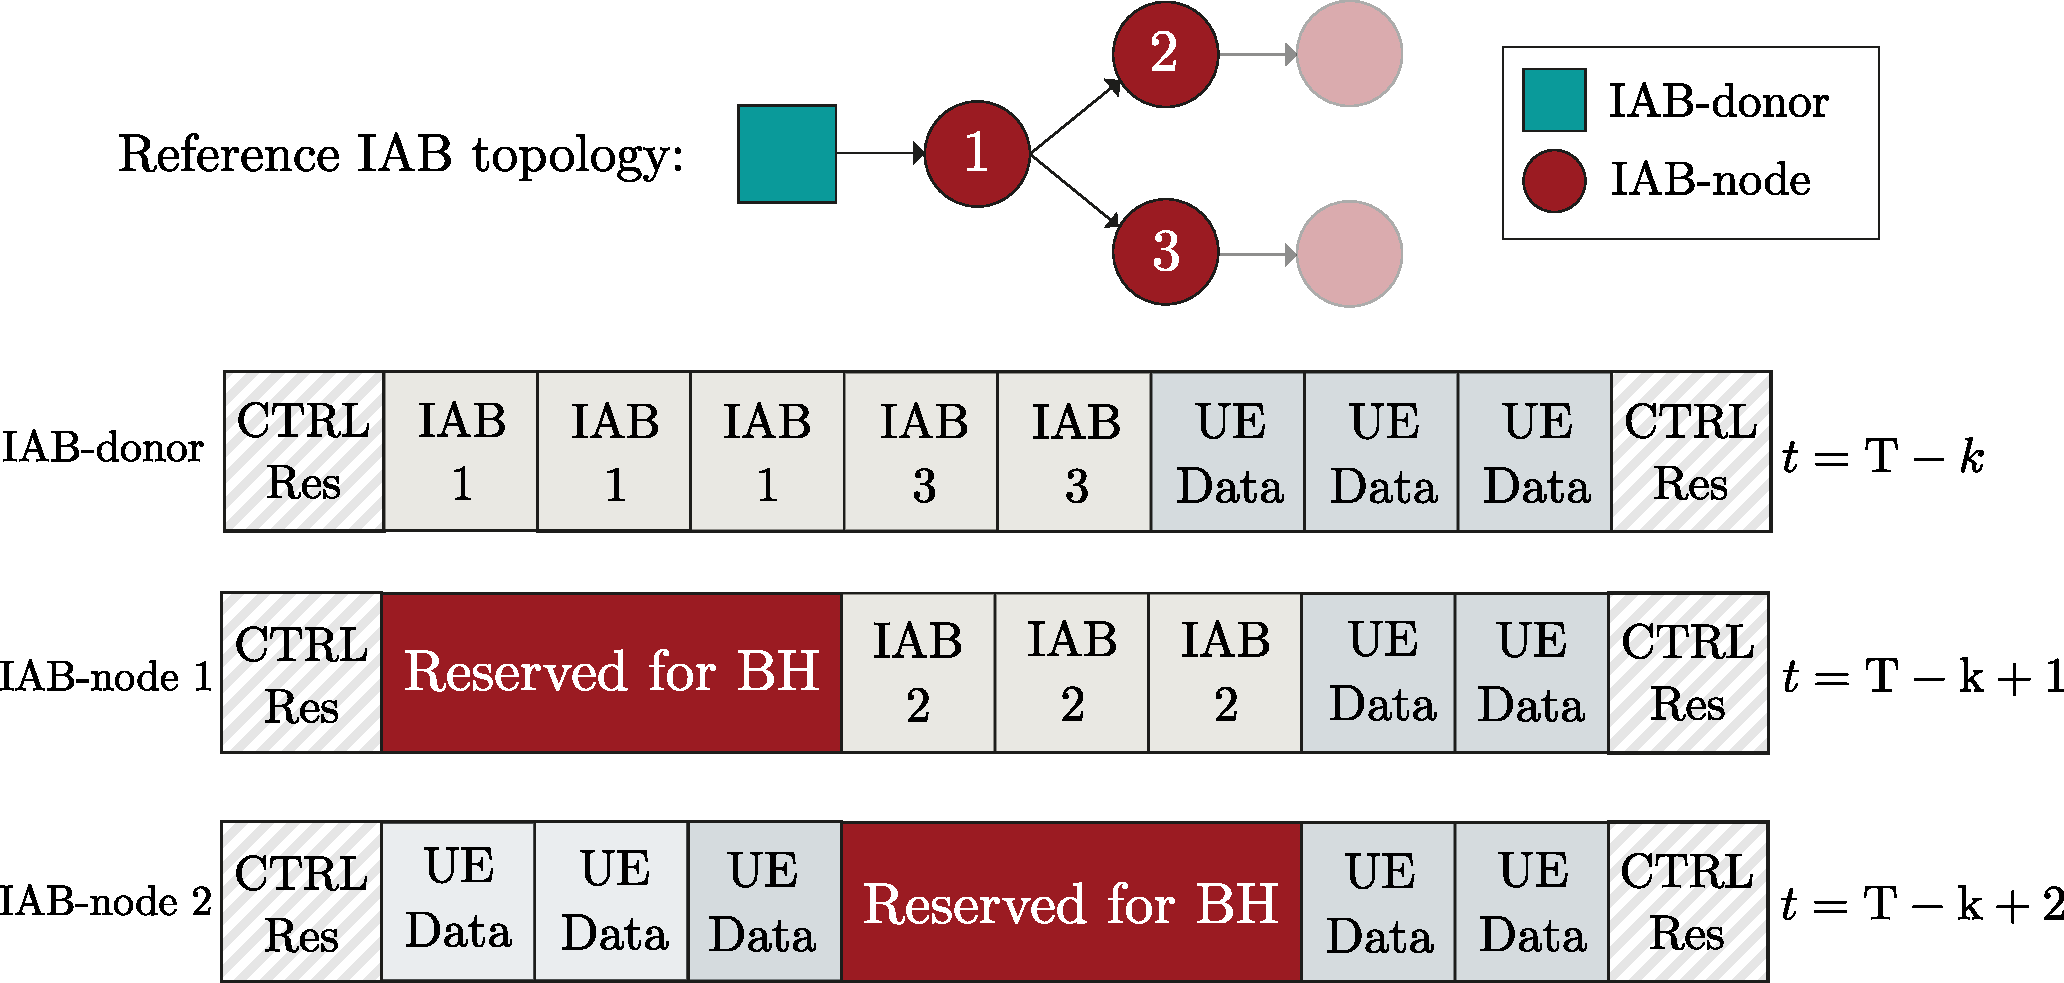
\includegraphics[width=0.75\linewidth]{IabSchedAlloc.pdf}
%\caption{Baseline distributed scheduler: example of a resource allocation at time $T$, for the depicted reference topology and where $k - 1$ indicates the maximum depth in the \gls{iab} network. Figure adapted from~\cite{polese2018end}.}
%\label{Fig:iab_sched_alloc}
%\vspace{-.6cm}
%\end{figure}

%An example of this scheduling mechanism is depicted in Fig.~\ref{Fig:iab_sched_alloc}: it can be noted how, for instance, the time resources which the donor has scheduled for backhauling purposes towards \gls{iab}-node 1 are marked as reserved by the latter. As a consequence, such node constraints its resource allocation to the remaining time slots only. 

\subsection{Simulation scenario and parameters}
The purpose of these simulations is to understand the performance of the proposed resource partitioning framework in the context of its target deployment, i.e., a multi-hop \gls{iab} network. As a consequence, the reference scenario consists of a dense urban deployment with a single \gls{iab}-donor and multiple \gls{iab}-nodes, as depicted in Fig.~\ref{Fig:Sim_scen}. In particular, the various \glspl{gnb} are distributed along an urban grid where the donor is located at the origin while the \gls{iab}-nodes are deployed along the street intersections, with a minimum inter-site distance of 100 m. The \gls{iab}-nodes attachments are computed using the so-called \textit{HQF} policy presented in~\cite{polese2018iab}; however, this choice does not introduce any loss of generality since such parameter is fixed for all the runs. A given number of \glspl{ue} are deployed within the surroundings of these base stations, with an initial position which is randomly sampled from circles of radius $\rho$ and whose centers are the various \glspl{gnb}. A summary of the simulation parameters in provided in Tab.~\ref{Tab:Sim_params}.
%Notably, the choice of not considering mobile \glspl{ue} is driven exclusively by concerns regarding the time needed to run our simulation campaigns. In fact, our framework introduces no limitations in such regard, due to the way the \gls{iab} topology is retrieved and the fact that we do not keep track of the per-flow information.
%The lack of mobility is mainly driven by concerns over the computational complexity of the simulations. 

\begin{figure}[tbp]
    \centering
    \subfloat[A realization of the simulation scenario; the dotted lines represent the cell-attachments of the \gls{iab}-nodes.\label{Fig:Sim_scen}]{
     % this sets the width of the figure, adjust to your needs
     \setlength\fwidth{0.7\columnwidth}
     % this sets the height of the figure, adjust to your needs
     \setlength\fheight{0.35\columnwidth}
       \raisebox{-.5\height}{\begin{tikzpicture}

    \definecolor{UNIPDRED}{RGB}{155,0,20}
	\definecolor{COMPLEMENTARY}{RGB}{0,153,153}
	\definecolor{DARKGREY}{RGB}{55,65,64}
	\definecolor{BLACK}{RGB}{20, 20, 20}
    
    \begin{axis}[
    width=\fwidth,
    height=\fheight,
    at={(0\fwidth,0\fheight)},
    scale only axis,
    legend style={
    	/tikz/every even column/.append style={column sep=0.3cm},
    	at={(0.5,0.98)},
    	anchor=south, 
    	draw=white!80!black, 
    	font=\small
    	},
    legend columns=3,
    %axis line style={white!80!black},
    %tick align=outside,
    %x grid style={white!80!black},
    xlabel style={font=\footnotesize},
    xlabel={},
    xtick={-100, -50, 0, 50, 100, 150},
    xmajorgrids,
    %xmajorticks=false,
    xmin=-150, xmax=150,
    xtick style={color=white!15!black},
    %y grid style={white!80!black},
    ylabel style={font=\footnotesize},
    ylabel={},
    ymajorgrids,
    %ymajorticks=false,
    ymin=-50, ymax=150,
    ytick style={color=white!15!black}
	]
	
	% IAB-node attachments
	\addplot[very thick, UNIPDRED, forget plot, dash pattern=on 5 pt off 3 pt] 
	table {%
	-100 0 
	0 0 
	};
	\addplot[very thick, UNIPDRED, forget plot, dash pattern=on 5 pt off 3 pt] 
	table {%
	100 100 
	0 0 
	};
	\addplot[very thick, UNIPDRED, forget plot, dash pattern=on 5 pt off 3 pt] 
	table {%
	-100 100 
	0 0 
	};
	\addplot[very thick, UNIPDRED, forget plot, dash pattern=on 5 pt off 3 pt] 
	table {%
	100 0 
	100 100 
	};
	\addplot[very thick, UNIPDRED, forget plot, dash pattern=on 5 pt off 3 pt] 
	table {%
	0 100 
	-100 100 
	};

    \addplot[
      scatter,
      only marks,
      scatter src=explicit,
      scatter/classes={1={DARKGREY, mark=square*}, 2={UNIPDRED, mark=diamond*}, 3={COMPLEMENTARY}},
      visualization depends on=\thisrow{sizedata}\as\sizedata,
      scatter/@pre marker code/.append style={
          /tikz/mark size=\sizedata
      }
    ]
    table[x=x,y=y, meta=class]{%
    x                      y                      sizedata                class
    0 0 5 1 
	100 0 6 2 
	-100 0 6 2 
	0 100 6 2 
	100 100 6 2 
	-100 100 6 2 
	28.8603 6.70813 2 3 
	22.1839 0.179283 2 3 
	-25.8695 -4.74675 2 3 
	-25.698 1.31045 2 3 
	-26.1185 5.61727 2 3 
	-18.8974 12.8042 2 3 
	-25.8278 8.77018 2 3 
	-11.9403 24.625 2 3 
	86.2329 -14.9938 2 3 
	113.411 -25.4381 2 3 
	80.796 10.6876 2 3 
	89.0457 9.21925 2 3 
	87.952 27.3012 2 3 
	89.4537 -0.761095 2 3 
	108.92 -15.5517 2 3 
	84.0229 -13.509 2 3 
	-71.3282 -2.49305 2 3 
	-114.738 26.7601 2 3 
	-115.867 28.3354 2 3 
	-117.757 24.2406 2 3 
	-103.439 -22.3846 2 3 
	-89.1148 5.80584 2 3 
	-116.494 -26.2217 2 3 
	-130.211 3.15653 2 3 
	-19.5929 85.0171 2 3 
	-22.2209 78.2847 2 3 
	13.0963 129.843 2 3 
	-15.409 112.165 2 3 
	-26.1002 118.747 2 3 
	12.3455 84.2945 2 3 
	-30.9925 96.9305 2 3 
	-33.7183 108.212 2 3 
	125.011 97.7272 2 3 
	112.293 126.281 2 3 
	113.959 76.0568 2 3 
	103.236 114.801 2 3 
	104.862 76.3655 2 3 
	131.206 109.996 2 3 
	114.825 128.336 2 3 
	90.7864 78.3714 2 3 
	-109.959 77.6437 2 3 
	-83.8184 115.384 2 3 
	-78.9347 82.8969 2 3 
	-114.208 81.4837 2 3 
	-123.238 80.8704 2 3 
	-104.259 88.5412 2 3 
	-94.1952 108.948 2 3 
	-114.781 80.0824 2 3 
    };
    \legend{\gls{iab}-donor, \gls{iab}-node, \gls{ue}}

    \end{axis}
    
\end{tikzpicture}




}
    }\hfill
    \subfloat[Simulation parameters.\label{Tab:Sim_params}]{
     \small
   \begin{tabular}{cc}
   \multicolumn{2}{c}{\textsc{Simulation parameters}}\\
   \hline
   \textsc{Parameter} & \textsc{Value} \\
   \hline
   Number of runs $N_{runs}$ & 25  \\
   \rowcolor{gray!15} Simulation time $T_{sim}$ & 3 s \\
   \gls{mwm} period $T_{alloc}$ & $\{ 1, 2, 4\}$ subframes \\
   \rowcolor{gray!15} Layer 4 protocol & $\{ $UDP, TCP$ \}$ \\
   UDP packet size $s_{UDP}$ & $\{50, 100, 200, 500 \}$ B \\
   \rowcolor{gray!15} Weight policy $f_u$ & $\{$\gls{msr}, \gls{ba}, \gls{mrba}$\}$ \\
   \hline
   \end{tabular}
    }
    \label{Float:Sim_scen_and_params}
    \caption{Simulation configuration.}
    \vspace{-.6cm}
\end{figure}

\section{Performance evaluation}
\label{Sec:perf_eval}

\begin{figure*}[tbp]
	\centering
	%\captionsetup{singlelinecheck=false, justification=justified}
  % this sets the width of the figure, adjust to your needs
  	\subfloat[$s_{UDP}$ = 100 B, i.e., \gls{udp} rate of 8 Mbps.\label{Fig:Thr_ECDF_100}]{
  	\setlength\fwidth{0.85\columnwidth}
    % this sets the height of the figure, adjust to your needs
    \setlength\fheight{0.33\columnwidth}
    % This file was created by tikzplotlib v0.9.4.
\begin{tikzpicture}

\pgfplotsset{every tick label/.append style={font=\footnotesize}}

\definecolor{UNIPDRED}{RGB}{155,0,20}
\definecolor{LIGHT_GREY}{RGB}{189,195,199}
\definecolor{COMPLEMENTARY}{RGB}{0,153,153}
\definecolor{DARKGREY}{RGB}{55,65,64}
\definecolor{SAND}{RGB}{180,160,135}

\begin{axis}[
width=\fwidth,
height=\fheight,
at={(0\fwidth,0\fheight)},
scale only axis,
%axis line style={white!80!black},
legend style={
    /tikz/every even column/.append style={column sep=0.2cm},
    at={(0.3,0.65)}, 
    anchor=south, 
    draw=white!80!black, 
    font=\scriptsize
    },
legend columns=2,
%tick align=outside,
%x grid style={white!80!black},
xlabel style={font=\footnotesize},
xlabel={UE throughput [Mbps]},
xtick={0, 1, 2, 3, 4, 5, 6, 7, 8},
xmajorgrids,
%xmajorticks=false,
xmin=0, xmax=8.5,
xtick style={color=white!15!black},
%y grid style={white!80!black},
ylabel shift = -1 pt,
ylabel style={font=\footnotesize},
ylabel={},
ymajorgrids,
%ymajorticks=false,
ymin=0, ymax=1.05,
ytick style={color=white!15!black},
ytick={0.2,0.4,0.6,0.8,1},
]

\addplot [very thick, SAND]
table {%
0.26964259147644 0
0.440404176712036 0.00265252590179443
0.609135508537292 0.00353670120239258
0.860332727432251 0.00442087650299072
1.0021516084671 0.00530505180358887
1.80407619476318 0.00618922710418701
1.86674773693085 0.00707340240478516
1.86872935295105 0.0079575777053833
1.86899101734161 0.00972592830657959
1.86937344074249 0.012378454208374
1.87010157108307 0.0159151554107666
1.87021577358246 0.0194518566131592
2.07712340354919 0.0203360319137573
2.41580104827881 0.0212202072143555
2.42250800132751 0.0229885578155518
2.49782967567444 0.0238727331161499
2.49792218208313 0.0300618410110474
2.49854469299316 0.0309460163116455
2.49861669540405 0.0362510681152344
2.53574633598328 0.0371352434158325
2.62055969238281 0.0380194187164307
2.62811470031738 0.0389035940170288
2.6283221244812 0.039787769317627
2.62947773933411 0.0406719446182251
2.62970066070557 0.0415561199188232
2.63152194023132 0.0424402952194214
2.63152813911438 0.0442086458206177
2.63292241096497 0.0450928211212158
2.70582509040833 0.045976996421814
2.7062041759491 0.0468611717224121
2.74750280380249 0.0477453470230103
2.74760341644287 0.052166223526001
2.74846625328064 0.0530503988265991
2.74853825569153 0.0557029247283936
2.75460028648376 0.0565871000289917
2.75477480888367 0.0592396259307861
2.7600576877594 0.0601238012313843
2.76282501220703 0.0610079765319824
2.76886248588562 0.0618921518325806
2.76891660690308 0.0654288530349731
2.77063202857971 0.0663130283355713
2.77686285972595 0.0671972036361694
2.77710485458374 0.0733864307403564
2.80236387252808 0.0742706060409546
2.8199348449707 0.0760389566421509
2.82017755508423 0.0822280645370483
2.85566520690918 0.0839964151382446
2.85595607757568 0.0901856422424316
2.8617091178894 0.0910698175430298
2.92173385620117 0.0919539928436279
2.92190027236938 0.0946065187454224
2.92191123962402 0.0963748693466187
2.92233276367188 0.0981432199478149
2.92234015464783 0.0999115705490112
2.92527842521667 0.100795745849609
2.92528581619263 0.101679921150208
2.9258246421814 0.102564096450806
2.929114818573 0.104332447052002
2.92912936210632 0.1052166223526
2.93662095069885 0.106100797653198
2.94025444984436 0.106984972953796
2.94139933586121 0.107869148254395
2.95004892349243 0.108753323554993
2.95006012916565 0.109637498855591
2.95263600349426 0.110521674156189
3.05221819877625 0.111405849456787
3.10105562210083 0.113174200057983
3.10163307189941 0.11494255065918
3.10173964500427 0.122015953063965
3.1021363735199 0.123784303665161
3.10239195823669 0.125552654266357
3.1034996509552 0.126436829566956
3.10382151603699 0.128205180168152
3.10409879684448 0.132626056671143
3.13609457015991 0.133510112762451
3.1746392250061 0.136162638664246
3.17652249336243 0.13881516456604
3.17669486999512 0.143236041069031
3.17720103263855 0.145004391670227
3.17746067047119 0.146772742271423
3.17749857902527 0.14854109287262
3.1819634437561 0.150309443473816
3.18213176727295 0.15296196937561
3.18215084075928 0.155614495277405
3.18521070480347 0.156498670578003
3.18546652793884 0.16268789768219
3.18967056274414 0.163572072982788
3.19050908088684 0.167108774185181
3.1905243396759 0.168877124786377
3.19163966178894 0.169761300086975
3.22586989402771 0.170645475387573
3.2259795665741 0.175950527191162
3.22825646400452 0.17683470249176
3.22887134552002 0.177718877792358
3.22895216941833 0.179487228393555
3.22963714599609 0.180371403694153
3.22964477539062 0.18213963508606
3.23387002944946 0.183023929595947
3.23403215408325 0.185676336288452
3.23405933380127 0.189213037490845
3.24865412712097 0.190097212791443
3.25200819969177 0.190981388092041
3.26675033569336 0.191865563392639
3.26687836647034 0.195402264595032
3.26724529266357 0.200707316398621
3.26732730865479 0.202475666999817
3.2810640335083 0.203359842300415
3.28848099708557 0.204244017601013
3.31646943092346 0.205128192901611
3.33002424240112 0.206012368202209
3.44054198265076 0.206896543502808
3.44539618492126 0.207780718803406
3.44547009468079 0.211317420005798
3.4528751373291 0.212201595306396
3.45287919044495 0.213085770606995
3.45335388183594 0.213969945907593
3.45357251167297 0.217506647109985
3.45441627502441 0.219274997711182
3.45453190803528 0.223695874214172
3.45682525634766 0.225464224815369
3.46599340438843 0.226348400115967
3.49390959739685 0.227232575416565
3.49476051330566 0.228116750717163
3.49514007568359 0.234305858612061
3.49550652503967 0.236074209213257
3.50014185905457 0.237842559814453
3.50015044212341 0.238726854324341
3.50125217437744 0.239610910415649
3.50149917602539 0.242263436317444
3.50174760818481 0.24403178691864
3.50176906585693 0.248452663421631
3.50679159164429 0.249336838722229
3.50679588317871 0.250221014022827
3.50864505767822 0.251105189323425
3.51900315284729 0.25375771522522
3.52100944519043 0.254641890525818
3.52105116844177 0.255526065826416
3.52260971069336 0.256410241127014
3.52292323112488 0.260831117630005
3.52386355400085 0.261715292930603
3.52944040298462 0.264367818832397
3.52968239784241 0.266136169433594
3.52969074249268 0.267020344734192
3.53243970870972 0.26790452003479
3.53249073028564 0.268788695335388
3.53440809249878 0.273209571838379
3.53442907333374 0.275862097740173
3.53707981109619 0.27763044834137
3.54024815559387 0.279398798942566
3.54046893119812 0.283819675445557
3.63516759872437 0.284703731536865
3.67046523094177 0.286472082138062
3.70479202270508 0.287356376647949
3.77303051948547 0.288240432739258
3.77917289733887 0.289124727249146
3.77976870536804 0.290893077850342
3.78155207633972 0.29177713394165
3.78209376335144 0.292661428451538
3.78363299369812 0.293545484542847
3.78388023376465 0.295313835144043
3.7852737903595 0.296198010444641
3.79006505012512 0.297082185745239
3.79036831855774 0.302387237548828
3.79567718505859 0.304155588150024
3.80048441886902 0.305039763450623
3.80264544487 0.305923938751221
3.80306959152222 0.308576464653015
3.80311512947083 0.309460639953613
3.82224583625793 0.310344815254211
3.8991870880127 0.31122899055481
3.90082430839539 0.312113165855408
3.90106749534607 0.313881516456604
3.90127801895142 0.317418217658997
3.90210723876953 0.318302392959595
3.90306997299194 0.323607444763184
3.9030978679657 0.327144145965576
3.92078280448914 0.328912496566772
3.92103576660156 0.331565022468567
3.92293262481689 0.332449197769165
3.92621231079102 0.333333373069763
3.98159027099609 0.334217548370361
3.98194789886475 0.340406656265259
3.98215365409851 0.341290950775146
4.01277494430542 0.342175006866455
4.01874113082886 0.343059301376343
4.0387282371521 0.343943357467651
4.05502891540527 0.345711708068848
4.16511964797974 0.346596002578735
4.17559957504272 0.347480058670044
4.23066568374634 0.348364353179932
4.24002552032471 0.350132584571838
4.27321434020996 0.351016759872437
4.2744312286377 0.352785110473633
4.27443647384644 0.353669285774231
4.30599355697632 0.354553461074829
4.3209490776062 0.355437636375427
4.3435754776001 0.356321811676025
4.58782386779785 0.358090162277222
4.64074563980103 0.359858512878418
4.64150619506836 0.362511038780212
4.64165592193604 0.363395214080811
4.64242935180664 0.365163564682007
4.64243507385254 0.366047739982605
4.72712326049805 0.366931915283203
4.72848701477051 0.371352791786194
4.72852659225464 0.37312114238739
4.73176956176758 0.374005317687988
4.73201608657837 0.374889492988586
4.73816013336182 0.375773668289185
4.99486064910889 0.376657843589783
4.99780225753784 0.377542018890381
4.9992036819458 0.378426194190979
4.99922752380371 0.379310369491577
5.00031185150146 0.380194544792175
5.00619983673096 0.381078720092773
5.00699758529663 0.38284707069397
5.00713300704956 0.386383771896362
5.00887537002563 0.389036178588867
5.00924777984619 0.39257287979126
5.0092716217041 0.393457174301147
5.01016283035278 0.396109580993652
5.36077451705933 0.397877931594849
5.45640563964844 0.398762226104736
5.59347248077393 0.399646282196045
5.59372854232788 0.404951333999634
5.71079158782959 0.405835509300232
5.71807241439819 0.40671968460083
5.71811294555664 0.407603859901428
5.71947479248047 0.408488035202026
5.71977233886719 0.409372210502625
5.9135046005249 0.410256385803223
5.95501756668091 0.411140561103821
5.96454858779907 0.412024736404419
5.96482753753662 0.413793087005615
5.96508502960205 0.41644561290741
5.98064374923706 0.417329788208008
6.34759044647217 0.418213963508606
6.48497629165649 0.419982314109802
6.4860372543335 0.4208664894104
6.48632860183716 0.425287365913391
6.48778867721558 0.426171541213989
6.50417757034302 0.427055716514587
6.50450038909912 0.428824067115784
6.504554271698 0.432360768318176
6.53208923339844 0.433244943618774
6.53364706039429 0.435013294219971
6.53366279602051 0.435897469520569
6.71247386932373 0.437665820121765
6.71300649642944 0.438549995422363
6.85143709182739 0.439434170722961
6.85148572921753 0.44031834602356
6.85364723205566 0.441202402114868
6.85380268096924 0.442970752716064
6.87466621398926 0.443855047225952
6.95184946060181 0.444739103317261
6.96869039535522 0.446507453918457
6.96899509429932 0.450928449630737
6.97008609771729 0.451812505722046
7.01210975646973 0.452696800231934
7.01526260375977 0.453580856323242
7.02312421798706 0.45446503162384
7.02828359603882 0.456233382225037
7.02868795394897 0.458885908126831
7.03365659713745 0.459770083427429
7.03687238693237 0.461538434028625
7.03884840011597 0.463306784629822
7.03897762298584 0.465075135231018
7.04769659042358 0.467727661132812
7.04871797561646 0.470380187034607
7.04896020889282 0.476569414138794
7.06435680389404 0.477453589439392
7.06582593917847 0.47833776473999
7.06814908981323 0.479221940040588
7.06824493408203 0.480106115341187
7.07024717330933 0.480990290641785
7.07034254074097 0.483642816543579
7.10552263259888 0.484526991844177
7.10553121566772 0.485411167144775
7.12034606933594 0.486295342445374
7.12035465240479 0.487179517745972
7.12568378448486 0.48806369304657
7.12577247619629 0.488947868347168
7.12878942489624 0.491600394248962
7.12909984588623 0.494252920150757
7.12917041778564 0.496905326843262
7.19264221191406 0.498673677444458
7.19721364974976 0.499557971954346
7.19817972183228 0.500442028045654
7.19826078414917 0.504863023757935
7.20064449310303 0.505747079849243
7.20089721679688 0.507515430450439
7.20201778411865 0.508399724960327
7.20212602615356 0.512820482254028
7.20610332489014 0.513704657554626
7.27363061904907 0.514588832855225
7.27442312240601 0.515473008155823
7.27444124221802 0.517241358757019
7.2751145362854 0.518125534057617
7.27545595169067 0.520778059959412
7.27801990509033 0.52166223526001
7.27887773513794 0.522546410560608
7.2790994644165 0.528735637664795
7.28205442428589 0.529619812965393
7.28302431106567 0.530503988265991
7.28306102752686 0.531388163566589
7.36370086669922 0.532272338867188
7.36590242385864 0.533156514167786
7.42193555831909 0.534924864768982
7.42232847213745 0.537577390670776
7.54834079742432 0.538461565971375
7.54871797561646 0.540229797363281
7.54880714416504 0.544650793075562
7.68753862380981 0.54553484916687
7.75189876556396 0.547303199768066
7.7585825920105 0.548187494277954
7.7586555480957 0.554376602172852
7.78432655334473 0.555260896682739
7.78829669952393 0.556144952774048
7.78843402862549 0.55968165397644
7.80472946166992 0.560565948486328
7.80569553375244 0.562334299087524
7.805748462677 0.566755056381226
7.84723281860352 0.567639231681824
7.84967947006226 0.571175932884216
7.84972238540649 0.573828458786011
7.88307237625122 0.574712634086609
7.88419818878174 0.575596809387207
7.88420915603638 0.576480984687805
7.88542222976685 0.5791335105896
7.88546514511108 0.580901861190796
7.90265941619873 0.581786036491394
7.93057441711426 0.582670211791992
7.93491506576538 0.58355438709259
7.93495893478394 0.587091088294983
7.93593549728394 0.587975263595581
7.93594646453857 0.588859438896179
7.94893455505371 0.589743614196777
7.9490761756897 0.590627789497375
7.94977140426636 0.591511964797974
7.95147800445557 0.592396020889282
7.95183038711548 0.59328031539917
7.9531192779541 0.594164371490479
7.95380258560181 0.596817016601562
7.9541220664978 0.599469423294067
7.95531272888184 0.600353717803955
7.95600700378418 0.602122068405151
7.95806932449341 0.60300612449646
7.95811367034912 0.603890419006348
7.95934963226318 0.604774475097656
7.95951461791992 0.606542825698853
7.9607720375061 0.60742712020874
7.96089458465576 0.608311176300049
7.96199893951416 0.609195470809937
7.96215343475342 0.615384578704834
7.96322441101074 0.616268873214722
7.9634895324707 0.622457981109619
7.96455001831055 0.623342156410217
7.96477127075195 0.627763032913208
7.96508073806763 0.629531383514404
7.96534585952759 0.633952260017395
7.96560001373291 0.635720610618591
7.96586561203003 0.640141487121582
7.96607542037964 0.641909837722778
7.9674243927002 0.780725002288818
7.96773386001587 0.887709975242615
7.96797704696655 0.889478325843811
7.96834135055542 0.897435903549194
7.96849679946899 0.900972604751587
7.96870708465576 0.946065425872803
7.96904993057251 0.999115824699402
8.5 1
};
\addlegendentry{Distr}


\addplot [very thick, COMPLEMENTARY, mark=square*, mark repeat=60, mark phase=40]
table {%
0.000693440437316895 0
0.119515538215637 0.000922560691833496
0.159256935119629 0.00184500217437744
0.597056031227112 0.00461256504058838
0.712712645530701 0.00553500652313232
0.726806163787842 0.00645756721496582
0.726821184158325 0.0119925737380981
0.759883642196655 0.0129151344299316
0.760014295578003 0.0193727016448975
0.992992997169495 0.0202951431274414
1.00686490535736 0.0212177038192749
1.00782418251038 0.0221402645111084
1.0082551240921 0.0276752710342407
1.07422256469727 0.0285978317260742
1.23650026321411 0.0295202732086182
1.24447298049927 0.0304428339004517
1.24472653865814 0.0341328382492065
1.25939452648163 0.03505539894104
1.26051843166351 0.035977840423584
1.3560699224472 0.0369004011154175
1.37027359008789 0.0387454032897949
1.37027680873871 0.0396678447723389
1.37143182754517 0.0405904054641724
1.37257981300354 0.0424354076385498
1.3732488155365 0.0433579683303833
1.44303858280182 0.0442804098129272
1.44760024547577 0.0452029705047607
1.44767200946808 0.0553505420684814
1.44881331920624 0.0562731027603149
1.44886040687561 0.0581181049346924
1.4539886713028 0.0599631071090698
1.45400047302246 0.0636531114578247
1.46569454669952 0.0645756721496582
1.5681084394455 0.0654981136322021
1.56836795806885 0.0673432350158691
1.56838297843933 0.071955680847168
1.9457221031189 0.0728782415390015
1.94600713253021 0.0747232437133789
1.946009516716 0.0756458044052124
1.94791996479034 0.0765682458877563
1.9479501247406 0.0784132480621338
1.95214557647705 0.0793358087539673
1.95215487480164 0.0830258131027222
1.95394539833069 0.0839483737945557
1.95394778251648 0.0848708152770996
1.99196577072144 0.0857933759689331
2.00361347198486 0.0867158174514771
2.02677488327026 0.0876383781433105
2.03139662742615 0.088560938835144
2.03273844718933 0.089483380317688
2.03275299072266 0.0913283824920654
2.03436756134033 0.0922509431838989
2.11717700958252 0.0931733846664429
2.12111163139343 0.0940959453582764
2.12173199653625 0.0959409475326538
2.12183690071106 0.104243516921997
2.12198424339294 0.106088519096375
2.12270855903625 0.107011079788208
2.12271428108215 0.108856081962585
2.1304190158844 0.109778642654419
2.13463735580444 0.110701084136963
2.13466668128967 0.113468647003174
2.13652753829956 0.114391088485718
2.18809390068054 0.116236209869385
2.1887571811676 0.117158651351929
2.18899250030518 0.122693777084351
2.21482110023499 0.123616218566895
2.21729159355164 0.125461220741272
2.22486162185669 0.126383781433105
2.22808194160461 0.127306222915649
2.22856187820435 0.128228783607483
2.23040413856506 0.129151344299316
2.26028728485107 0.13007378578186
2.26797556877136 0.130996346473694
2.26861238479614 0.136531352996826
2.27123975753784 0.13745391368866
2.36648774147034 0.138376355171204
2.36989164352417 0.139298915863037
2.37159609794617 0.140221357345581
2.37233400344849 0.142988920211792
2.37260818481445 0.143911480903625
2.41940212249756 0.144833922386169
2.41964530944824 0.145756483078003
2.42206501960754 0.146678924560547
2.42693829536438 0.14760148525238
2.42717909812927 0.151291489601135
2.4275426864624 0.152214050292969
2.42995262145996 0.153136491775513
2.43535137176514 0.154059052467346
2.43768572807312 0.15498161315918
2.44726800918579 0.155904054641724
2.46195650100708 0.156826615333557
2.46219205856323 0.160516619682312
2.46288466453552 0.161439180374146
2.46297359466553 0.163284182548523
2.46382284164429 0.164206624031067
2.47657942771912 0.1651291847229
2.47667551040649 0.166051626205444
2.47775530815125 0.166974186897278
2.47780537605286 0.169741630554199
2.49199962615967 0.170664191246033
2.4981062412262 0.171586751937866
2.49834179878235 0.174354195594788
2.49867010116577 0.176199197769165
2.49881720542908 0.178966760635376
2.4992470741272 0.180811762809753
2.49961495399475 0.184501886367798
2.50682592391968 0.185424327850342
2.50773572921753 0.187269330024719
2.50836801528931 0.188191890716553
2.50860404968262 0.196494460105896
2.50996613502502 0.197417020797729
2.51020765304565 0.199262022972107
2.52322888374329 0.202952027320862
2.52448034286499 0.204797029495239
2.52550864219666 0.205719590187073
2.52551198005676 0.206642031669617
2.52628231048584 0.20756459236145
2.53637742996216 0.208487033843994
2.53685307502747 0.209409594535828
2.53725171089172 0.215867161750793
2.53755116462708 0.217712163925171
2.5375611782074 0.220479726791382
2.54133033752441 0.221402168273926
2.54211711883545 0.223247289657593
2.54214453697205 0.22509229183197
2.54261207580566 0.226014733314514
2.55435681343079 0.226937294006348
2.55480432510376 0.227859735488892
2.55734658241272 0.228782296180725
2.57158017158508 0.230627298355103
2.57307934761047 0.231549859046936
2.58276295661926 0.234317302703857
2.58307123184204 0.235239863395691
2.584144115448 0.236162424087524
2.59009289741516 0.238929867744446
2.60104560852051 0.240774869918823
2.6070122718811 0.241697430610657
2.61967539787292 0.24261999130249
2.66720509529114 0.244464993476868
2.66725587844849 0.245387434959412
2.72790575027466 0.247232437133789
2.72818279266357 0.251845002174377
2.72862124443054 0.252767562866211
2.73049545288086 0.253690004348755
2.73609709739685 0.255535125732422
2.736483335495 0.259225130081177
2.73679137229919 0.261992692947388
2.81280612945557 0.263837575912476
2.83584880828857 0.264760136604309
2.83783507347107 0.265682697296143
2.95929646492004 0.269372701644897
2.96097469329834 0.270295143127441
2.96567916870117 0.271217703819275
2.96619153022766 0.272140264511108
2.96729707717896 0.273062705993652
2.96801328659058 0.27490770816803
2.96865940093994 0.275830268859863
2.96866989135742 0.276752710342407
2.97192597389221 0.277675271034241
2.97657895088196 0.280442833900452
2.99721527099609 0.282287836074829
3.0449481010437 0.284132838249207
3.04524064064026 0.290590405464172
3.05891418457031 0.291512966156006
3.05913615226746 0.29243540763855
3.09333443641663 0.293357968330383
3.10531139373779 0.295202970504761
3.16781735420227 0.296125411987305
3.18863844871521 0.297047972679138
3.18915510177612 0.297970533370972
3.18941736221313 0.303505539894104
3.18967962265015 0.305350542068481
3.18969559669495 0.309040546417236
3.19570779800415 0.30996310710907
3.19670009613037 0.310885667800903
3.19858813285828 0.311808109283447
3.2024610042572 0.312730669975281
3.20366549491882 0.313653111457825
3.20367336273193 0.314575672149658
3.20530080795288 0.315498113632202
3.20531678199768 0.316420674324036
3.36194229125977 0.317343235015869
3.42266368865967 0.318265676498413
3.42354035377502 0.320110678672791
3.42375755310059 0.324723243713379
3.50149536132812 0.325645685195923
3.51525497436523 0.326568245887756
3.56066226959229 0.328413248062134
3.56259059906006 0.330258369445801
3.5631160736084 0.331180810928345
3.56805229187012 0.332103252410889
3.568204164505 0.333948373794556
3.5710117816925 0.3348708152771
3.57147884368896 0.336715936660767
3.58437633514404 0.337638378143311
3.58603763580322 0.338560819625854
3.58673048019409 0.340405941009521
3.58921003341675 0.342250943183899
3.60637378692627 0.343173503875732
3.61262488365173 0.344095945358276
3.62165451049805 0.34501838684082
3.6219437122345 0.349630951881409
3.62346935272217 0.350553512573242
3.6261613368988 0.351475954055786
3.62666988372803 0.35239851474762
3.63200402259827 0.354243516921997
3.63224840164185 0.356088519096375
3.63386368751526 0.357011079788208
3.68670630455017 0.357933521270752
3.69633603096008 0.358856081962585
3.69879579544067 0.359778642654419
3.72128319740295 0.360701084136963
3.72143459320068 0.361623644828796
3.74851179122925 0.36254608631134
3.75784826278687 0.363468647003174
3.75816464424133 0.365313649177551
3.75844478607178 0.369003653526306
3.7591495513916 0.36992621421814
3.75941681861877 0.374538779258728
3.76022744178772 0.375461220741272
3.79992628097534 0.376383781433105
3.80160331726074 0.377306222915649
3.85554623603821 0.38007378578186
3.876544713974 0.380996346473694
3.94954562187195 0.381918787956238
4.02695846557617 0.383763790130615
4.09507656097412 0.384686350822449
4.12194061279297 0.386531352996826
4.14429044723511 0.38745391368866
4.35945320129395 0.390221357345581
4.35966157913208 0.392066478729248
4.36110973358154 0.392988920211792
4.36112546920776 0.393911480903625
4.39790821075439 0.395756483078003
4.4080286026001 0.396678924560547
4.41130590438843 0.39760148525238
4.87467813491821 0.398524045944214
4.9422812461853 0.399446487426758
4.95907831192017 0.400369048118591
4.96778535842896 0.402214050292969
4.97122573852539 0.403136491775513
4.97210836410522 0.404059052467346
4.97302675247192 0.407749056816101
4.98327779769897 0.408671617507935
5.00254821777344 0.409594058990479
5.00930595397949 0.410516619682312
5.0093297958374 0.412361621856689
5.01085090637207 0.413284063339233
5.04663467407227 0.414206624031067
5.13907670974731 0.4151291847229
5.34705781936646 0.416051626205444
5.34793853759766 0.416974186897278
5.35226726531982 0.417896747589111
5.38592481613159 0.418819189071655
5.38914728164673 0.419741630554199
5.39950656890869 0.420664191246033
5.42634010314941 0.421586751937866
5.45551300048828 0.423431754112244
5.55426406860352 0.424354314804077
5.55430364608765 0.427121758460999
5.63289642333984 0.428044319152832
6.02040863037109 0.430811882019043
6.02500772476196 0.431734323501587
6.08387899398804 0.432656764984131
6.73705244064331 0.433579325675964
6.74483633041382 0.434501886367798
6.74887037277222 0.435424327850342
6.7491021156311 0.439114332199097
6.85364723205566 0.440959453582764
6.85635662078857 0.441881895065308
6.87699699401855 0.444649457931519
6.87701320648193 0.445571899414062
6.87871122360229 0.446494460105896
6.8796010017395 0.447417020797729
6.88149785995483 0.448339462280273
6.88155555725098 0.450184464454651
6.88558340072632 0.451107025146484
6.88758230209351 0.452029466629028
6.89099740982056 0.452952027320862
6.89266014099121 0.453874588012695
6.89994239807129 0.454797029495239
6.90160942077637 0.456642031669617
6.91130590438843 0.45756459236145
6.9207124710083 0.459409594535828
6.92298269271851 0.461254596710205
6.9279203414917 0.462177157402039
6.95650482177734 0.463099598884583
6.95882415771484 0.464022159576416
6.97282075881958 0.46494460105896
6.98741865158081 0.466789722442627
6.98815011978149 0.467712163925171
7.00506782531738 0.468634724617004
7.00670099258423 0.469557166099548
7.00720548629761 0.472324728965759
7.00770139694214 0.473247289657593
7.00770998001099 0.474169731140137
7.00936126708984 0.47509229183197
7.01292324066162 0.476014733314514
7.0336480140686 0.477859735488892
7.05020666122437 0.478782296180725
7.05145359039307 0.479704856872559
7.06788778305054 0.480627298355103
7.07065629959106 0.481549859046936
7.07211971282959 0.48247230052948
7.08277320861816 0.483394861221313
7.08382177352905 0.484317302703857
7.08559703826904 0.485239863395691
7.08585929870605 0.486162424087524
7.08767032623291 0.487084865570068
7.08778381347656 0.488007307052612
7.09101438522339 0.489852428436279
7.0950984954834 0.490774869918823
7.09628248214722 0.491697430610657
7.09643125534058 0.494464874267578
7.09959077835083 0.497232437133789
7.10164594650269 0.498154997825623
7.10471343994141 0.499077558517456
7.10477495193481 0.5
7.12326955795288 0.500922441482544
7.1237211227417 0.501845002174377
7.12589645385742 0.502767562866211
7.1291880607605 0.503690004348755
7.13091468811035 0.505535125732422
7.13128709793091 0.506457567214966
7.13555908203125 0.50738000869751
7.13758230209351 0.508302569389343
7.13759994506836 0.510147571563721
7.1408314704895 0.511070132255554
7.1425461769104 0.513837575912476
7.16809701919556 0.514760136604309
7.17349863052368 0.515682697296143
7.17351627349854 0.516605138778687
7.19400310516357 0.518450260162354
7.19401216506958 0.519372701644897
7.20268630981445 0.520295143127441
7.20301151275635 0.522140264511108
7.21727418899536 0.523062705993652
7.21957015991211 0.523985266685486
7.21958827972412 0.525830268859863
7.31250619888306 0.526752710342407
7.31355905532837 0.527675271034241
7.31362438201904 0.528597831726074
7.31456565856934 0.529520273208618
7.3147144317627 0.533210277557373
7.37175703048706 0.534132838249207
7.37609481811523 0.53505539894104
7.3762845993042 0.537822961807251
7.37632274627686 0.540590405464172
7.55123043060303 0.541512966156006
7.55334615707397 0.54243540763855
7.58306884765625 0.543357849121094
7.5868067741394 0.544280529022217
7.59393215179443 0.545202970504761
7.59402275085449 0.547970533370972
7.61951303482056 0.548892974853516
7.62096929550171 0.54981541633606
7.62558555603027 0.550738096237183
7.62667989730835 0.551660537719727
7.62693309783936 0.555350542068481
7.68902111053467 0.556272983551025
7.72382164001465 0.557195544242859
7.74306344985962 0.558118104934692
7.74579000473022 0.559040546417236
7.75875043869019 0.55996310710907
7.76130962371826 0.560885667800903
7.76247453689575 0.561808109283447
7.76265287399292 0.563653111457825
7.79379463195801 0.564575672149658
7.79404878616333 0.565498113632202
7.79484272003174 0.566420674324036
7.79517078399658 0.571033239364624
7.8927321434021 0.571955680847168
7.9016695022583 0.572878241539001
7.90321445465088 0.579335808753967
7.93168115615845 0.582103252410889
7.95135688781738 0.583025813102722
7.95372581481934 0.583948373794556
7.95413303375244 0.586715936660767
7.95533466339111 0.588560819625854
7.95557737350464 0.590405941009521
7.95690059661865 0.591328382492065
7.95977973937988 0.596863508224487
7.96177816390991 0.598708510398865
7.96199893951416 0.601475954055786
7.96295928955078 0.60239851474762
7.9632134437561 0.604243516921997
7.9634895324707 0.608856081962585
7.96401882171631 0.609778642654419
7.96428489685059 0.611623644828796
7.96455001831055 0.613468647003174
7.96551084518433 0.630996227264404
7.9656777381897 0.633763790130615
7.96746826171875 0.816420674324036
7.96772289276123 0.867158651351929
7.96796607971191 0.869003772735596
7.96837425231934 0.876383781433105
7.96856355667114 0.879151344299316
7.96865224838257 0.917896747589111
7.96897268295288 0.999077558517456
8.5 1
};
\addlegendentry{\gls{msr}}

\addplot [very thick, DARKGREY, mark=*, mark repeat=60, mark phase=40]
table {%
0.234191179275513 0
0.281193256378174 0.00118064880371094
0.577000975608826 0.00236129760742188
0.63570237159729 0.00354194641113281
0.715597152709961 0.00472259521484375
2.6375572681427 0.00826442241668701
2.79069304466248 0.00944507122039795
2.88134479522705 0.0106257200241089
3.13204503059387 0.0118063688278198
3.14603781700134 0.0129870176315308
3.27042412757874 0.0141676664352417
3.65718984603882 0.0165289640426636
3.66828012466431 0.0177096128463745
3.85161876678467 0.0188901424407959
4.45079612731934 0.0212514400482178
4.52173185348511 0.0224320888519287
4.81968212127686 0.0236127376556396
5.00756978988647 0.0247933864593506
5.12364816665649 0.0259740352630615
5.47601079940796 0.0271546840667725
5.55078983306885 0.0283353328704834
5.80145311355591 0.0306966304779053
5.80315160751343 0.0318771600723267
5.80337381362915 0.0389610528945923
5.82239866256714 0.0401417016983032
5.82262086868286 0.0460448265075684
5.8230938911438 0.0472254753112793
6.00642681121826 0.0484061241149902
6.12701177597046 0.0495867729187012
6.17299699783325 0.0507674217224121
6.17315292358398 0.053128719329834
6.17396926879883 0.0543093681335449
6.17413330078125 0.0590318441390991
6.19868755340576 0.0602124929428101
6.19936847686768 0.061393141746521
6.20334625244141 0.0625737905502319
6.20465517044067 0.0637544393539429
6.20956516265869 0.0649350881576538
6.20965385437012 0.0672963857650757
6.22274255752563 0.0684769153594971
6.22341108322144 0.0708382129669189
6.22371101379395 0.0767414569854736
6.2290415763855 0.0779221057891846
6.23125219345093 0.0791027545928955
6.23155546188354 0.0861865282058716
6.2318000793457 0.0885478258132935
6.23534774780273 0.0897284746170044
6.23544311523438 0.0968122482299805
6.24525499343872 0.0979928970336914
6.24762630462646 0.0991735458374023
6.24795055389404 0.109799265861511
6.24859094619751 0.110979914665222
6.24881458282471 0.114521861076355
6.24885940551758 0.115702509880066
6.30343389511108 0.116883158683777
6.49414300918579 0.118063807487488
6.49481868743896 0.123966932296753
6.4948263168335 0.125147581100464
6.49542331695557 0.126328229904175
6.49547004699707 0.133412003517151
6.49991273880005 0.134592652320862
6.50055313110352 0.135773301124573
6.50082921981812 0.142857193946838
6.50360870361328 0.14403772354126
6.50397443771362 0.152302265167236
6.50939321517944 0.153482913970947
6.51118469238281 0.154663562774658
6.51146125793457 0.160566687583923
6.51471042633057 0.161747336387634
6.51506376266479 0.170011758804321
6.54694223403931 0.171192407608032
6.54775238037109 0.172373056411743
6.54802846908569 0.179456949234009
6.54883432388306 0.18063759803772
6.54892778396606 0.186540722846985
6.60878324508667 0.187721371650696
6.61003971099854 0.188902020454407
6.61057043075562 0.190082669258118
6.61864233016968 0.191263318061829
6.62090349197388 0.19244396686554
6.62114858627319 0.193624496459961
6.62281608581543 0.194805145263672
6.62286376953125 0.197166442871094
6.62870597839355 0.198347091674805
6.63044548034668 0.200708389282227
6.63075733184814 0.203069686889648
6.63173198699951 0.204250335693359
6.63178730010986 0.210153460502625
6.63322639465332 0.211334109306335
6.63388299942017 0.21723735332489
6.63473892211914 0.218417882919312
6.63480234146118 0.221959829330444
6.63534879684448 0.223140478134155
6.6353645324707 0.224321126937866
6.64044427871704 0.225501775741577
6.65826416015625 0.226682424545288
6.65831184387207 0.227863073348999
6.65894508361816 0.22904372215271
6.66067028045654 0.230224370956421
6.66130256652832 0.231405019760132
6.66305732727051 0.232585549354553
6.6633939743042 0.247933864593506
6.66427230834961 0.249114513397217
6.66447782516479 0.25265645980835
6.66450977325439 0.256198406219482
6.66619348526001 0.257379055023193
6.66637659072876 0.264462828636169
6.70076084136963 0.26564347743988
6.72005796432495 0.266824126243591
6.72196578979492 0.268004655838013
6.72199821472168 0.271546602249146
6.7226676940918 0.272727251052856
6.72272443771362 0.280991792678833
6.76421022415161 0.282172441482544
6.76430892944336 0.284533619880676
6.78140926361084 0.285714268684387
6.7816948890686 0.293978691101074
6.79471206665039 0.295159339904785
6.79652547836304 0.296339988708496
6.79733276367188 0.298701286315918
6.79770708084106 0.303423881530762
6.79794073104858 0.305785179138184
6.79798984527588 0.310507655143738
6.83917284011841 0.311688303947449
6.83949947357178 0.316410899162292
6.84021949768066 0.317591428756714
6.84061241149902 0.32585597038269
6.84079122543335 0.334120392799377
6.84119987487793 0.343565464019775
6.84451484680176 0.344746112823486
6.84469509124756 0.348288059234619
6.84473609924316 0.353010654449463
6.85029602050781 0.354191303253174
6.86941242218018 0.355371952056885
6.86956882476807 0.356552600860596
6.87249898910522 0.357733249664307
6.87255001068115 0.358913779258728
6.87306118011475 0.360094428062439
6.8731632232666 0.362455725669861
6.94546318054199 0.363636374473572
6.98510313034058 0.364817023277283
6.98515558242798 0.365997672080994
7.0257716178894 0.367178320884705
7.03333759307861 0.368358850479126
7.03713989257812 0.369539499282837
7.08486223220825 0.370720148086548
7.10189533233643 0.371900796890259
7.10194969177246 0.37308144569397
7.11906576156616 0.374262094497681
7.11914491653442 0.382526636123657
7.1237211227417 0.383707165718079
7.12441921234131 0.3860684633255
7.12495851516724 0.387249112129211
7.12517070770264 0.389610409736633
7.1262059211731 0.393152236938477
7.12664794921875 0.403778076171875
7.1276216506958 0.407320022583008
7.12770986557007 0.412042498588562
7.13669490814209 0.413223147392273
7.13941955566406 0.414403796195984
7.13985443115234 0.422668218612671
7.14984941482544 0.423848867416382
7.15009880065918 0.430932760238647
7.15110540390015 0.432113409042358
7.15116739273071 0.439197182655334
7.15798854827881 0.440377831459045
7.15889930725098 0.441558480262756
7.16438674926758 0.443919658660889
7.16461753845215 0.446280956268311
7.16466188430786 0.451003551483154
7.17371368408203 0.452184200286865
7.17488813400269 0.453364849090576
7.17522001266479 0.459267973899841
7.17820739746094 0.460448622703552
7.18009281158447 0.461629271507263
7.18014669418335 0.468713045120239
7.20384311676025 0.46989369392395
7.20500040054321 0.471074342727661
7.23035955429077 0.472254991531372
7.24466133117676 0.473435640335083
7.33897113800049 0.474616289138794
7.34754705429077 0.475796937942505
7.39095687866211 0.476977586746216
7.45756053924561 0.478158235549927
7.46381425857544 0.479338884353638
7.47392988204956 0.480519533157349
7.50526571273804 0.48170018196106
7.50832843780518 0.485242009162903
7.50846576690674 0.499409675598145
7.52174139022827 0.501770973205566
7.52270269393921 0.502951622009277
7.52311658859253 0.505312919616699
7.52316617965698 0.510035395622253
7.60781002044678 0.511216044425964
7.61590433120728 0.512396693229675
7.61735963821411 0.513577342033386
7.6306939125061 0.514757990837097
7.69751691818237 0.51829981803894
7.69755792617798 0.519480466842651
7.71661996841431 0.520661115646362
7.71698999404907 0.521841764450073
7.72263765335083 0.523022413253784
7.78663778305054 0.524203062057495
7.86779594421387 0.526564359664917
7.86843204498291 0.527745008468628
7.87892866134644 0.528925657272339
7.88024806976318 0.53010630607605
7.8803129196167 0.536009430885315
7.88176298141479 0.537190079689026
7.88681936264038 0.538370728492737
7.88808727264404 0.539551377296448
7.90061473846436 0.540731906890869
7.90190887451172 0.543093204498291
7.9021372795105 0.546635150909424
7.90217018127441 0.548996448516846
7.90732622146606 0.550177097320557
7.90760135650635 0.552538394927979
7.90763425827026 0.556080341339111
7.90927934646606 0.557260990142822
7.909508228302 0.561983466148376
7.91154670715332 0.563164114952087
7.92654466629028 0.564344763755798
7.92678546905518 0.566705942153931
7.92703723907471 0.569067239761353
7.92784738540649 0.573789834976196
7.92806625366211 0.574970483779907
7.93442153930664 0.577331781387329
7.93443250656128 0.57851243019104
7.93546342849731 0.579693078994751
7.93574857711792 0.587957501411438
7.93662691116333 0.589138150215149
7.9372410774231 0.605667114257812
7.93838262557983 0.609209060668945
7.93920612335205 0.610389590263367
7.93946981430054 0.617473363876343
7.94069957733154 0.618654012680054
7.94154500961304 0.623376607894897
7.94225931167603 0.624557256698608
7.94267702102661 0.636363625526428
7.94398498535156 0.637544274330139
7.94412755966187 0.642266750335693
7.94418287277222 0.645808696746826
7.94478750228882 0.648169994354248
7.9448094367981 0.649350643157959
7.9469633102417 0.65053129196167
7.94725131988525 0.652892589569092
7.947350025177 0.656434535980225
7.94893455505371 0.659976363182068
7.94911098480225 0.663518309593201
7.95081758499146 0.664698958396912
7.95102643966675 0.665879487991333
7.95203971862793 0.667060136795044
7.95210552215576 0.672963380813599
7.95310831069946 0.675324678421021
7.95315217971802 0.676505327224731
7.95422124862671 0.677685976028442
7.95472812652588 0.690672874450684
7.95573139190674 0.691853523254395
7.95621681213379 0.714285731315613
7.95686721801758 0.716646909713745
7.9571099281311 0.719008207321167
7.95713186264038 0.720188856124878
7.95761728286743 0.721369504928589
7.95803642272949 0.728453397750854
7.95841121673584 0.735537171363831
7.95880889892578 0.741440296173096
7.95950365066528 0.742620944976807
7.95974636077881 0.74734354019165
7.96004438400269 0.753246784210205
7.96132516860962 0.760330557823181
7.96170091629028 0.763872504234314
7.96247386932373 0.765053153038025
7.96277189254761 0.768594980239868
7.96335744857788 0.776859521865845
7.963942527771 0.778040170669556
7.96455001831055 0.811097979545593
7.9647159576416 0.815820455551147
7.96508073806763 0.824084997177124
7.96526861190796 0.827626943588257
7.96614170074463 0.883116960525513
7.96636295318604 0.886658787727356
7.96693754196167 0.914994120597839
7.9671368598938 0.918535947799683
7.96772289276123 0.956316471099854
7.96859693527222 0.961038947105408
7.96900606155396 0.998819351196289
8.5 1
};
\addlegendentry{\gls{ba}}


\addplot [very thick, UNIPDRED, mark=triangle*, mark repeat=60, mark phase=40]
table {%
0.12256932258606 0
0.38178026676178 0.00192868709564209
0.6866055727005 0.00289297103881836
0.736319899559021 0.00385725498199463
1.07956194877625 0.00482165813446045
1.16768050193787 0.00578594207763672
1.45352613925934 0.00675022602081299
1.61505031585693 0.00771450996398926
2.43438696861267 0.00867891311645508
2.66059112548828 0.0106074810028076
3.05167412757874 0.0125361680984497
3.48434042930603 0.013500452041626
3.49458479881287 0.0144648551940918
3.49554419517517 0.0192863941192627
3.49565052986145 0.020250678062439
3.70280957221985 0.0212150812149048
3.70297288894653 0.0260366201400757
3.72270226478577 0.0279653072357178
3.72906732559204 0.0318225622177124
3.7293119430542 0.0327868461608887
3.73013782501221 0.0337512493133545
3.73020911216736 0.035679817199707
3.7307014465332 0.0366442203521729
3.83266949653625 0.0376085042953491
3.84835004806519 0.0385727882385254
3.85103154182434 0.0395370721817017
3.85126495361328 0.0405014753341675
3.8830943107605 0.0414657592773438
3.96365022659302 0.04243004322052
4.09733200073242 0.0433944463729858
4.36823558807373 0.0443587303161621
4.43013715744019 0.0453230142593384
5.49280834197998 0.0472517013549805
5.49434328079224 0.0482159852981567
5.49438285827637 0.0540019273757935
5.80271148681641 0.0549662113189697
5.88212442398071 0.0559306144714355
6.13301181793213 0.0568948984146118
6.18410301208496 0.0578591823577881
6.19260692596436 0.0588235855102539
6.22052145004272 0.0597878694534302
6.22077322006226 0.0636451244354248
6.2208104133606 0.0655738115310669
6.2242431640625 0.0665380954742432
6.22893285751343 0.0703953504562378
6.22897005081177 0.0752170085906982
6.22946453094482 0.0761812925338745
6.22953128814697 0.0790742635726929
6.28768920898438 0.081002950668335
6.2915096282959 0.0819672346115112
6.29179906845093 0.0867887735366821
6.3637900352478 0.0877531766891479
6.54740047454834 0.0887174606323242
6.87631320953369 0.0896817445755005
6.88263607025146 0.0906461477279663
6.94804382324219 0.0916104316711426
6.95997142791748 0.0925747156143188
6.96118688583374 0.0935389995574951
6.96122884750366 0.0983606576919556
6.97293090820312 0.0993249416351318
6.97455739974976 0.100289344787598
6.97493886947632 0.107039570808411
6.97656631469727 0.108968138694763
6.97688865661621 0.112825512886047
6.97690534591675 0.113789796829224
6.98298168182373 0.116682767868042
6.98300743103027 0.11957573890686
7.01012277603149 0.120540022850037
7.01199865341187 0.121504306793213
7.01217794418335 0.122468709945679
7.01310348510742 0.124397277832031
7.01312065124512 0.126325964927673
7.01409721374512 0.12729024887085
7.01418304443359 0.134040474891663
7.06626987457275 0.135004758834839
7.08109569549561 0.135969161987305
7.08313131332397 0.136933445930481
7.08318376541138 0.141755104064941
7.08372592926025 0.143683671951294
7.0838041305542 0.149469614028931
7.12262487411499 0.150433897972107
7.13728904724121 0.151398301124573
7.13750219345093 0.154291272163391
7.13818597793579 0.155255556106567
7.1385669708252 0.159112811088562
7.1415867805481 0.160077095031738
7.14913749694824 0.161041498184204
7.153395652771 0.16200578212738
7.15441179275513 0.162970066070557
7.15459012985229 0.164898753166199
7.15547323226929 0.165863037109375
7.1556601524353 0.166827440261841
7.15975666046143 0.167791724205017
7.16074752807617 0.168756008148193
7.16340160369873 0.169720411300659
7.1739559173584 0.170684695243835
7.17997598648071 0.171648979187012
7.18257236480713 0.17454195022583
7.1835789680481 0.180327892303467
7.19634771347046 0.181292176246643
7.19651937484741 0.182256460189819
7.19730424880981 0.183220863342285
7.19738531112671 0.188042402267456
7.20851993560791 0.189006805419922
7.21453475952148 0.189971089363098
7.21678400039673 0.190935373306274
7.23643350601196 0.192864060401917
7.23693513870239 0.193828344345093
7.2688045501709 0.194792628288269
7.26904392242432 0.195757031440735
7.26973438262939 0.196721315383911
7.26975250244141 0.198650002479553
7.27026796340942 0.199614286422729
7.27027750015259 0.200578570365906
7.28007793426514 0.203471541404724
7.28308153152466 0.2044358253479
7.29841279983521 0.205400228500366
7.29923868179321 0.206364512443542
7.30019474029541 0.210221767425537
7.30038022994995 0.214079022407532
7.30067729949951 0.218900680541992
7.30645704269409 0.219864964485168
7.30730056762695 0.221793651580811
7.30752658843994 0.223722219467163
7.30756378173828 0.226615190505981
7.3110728263855 0.227579593658447
7.31156444549561 0.228543877601624
7.31193017959595 0.233365535736084
7.31496620178223 0.23432981967926
7.31791305541992 0.236258387565613
7.31819295883179 0.238187074661255
7.31832313537598 0.24204432964325
7.32328081130981 0.243008613586426
7.33352422714233 0.243973016738892
7.33376789093018 0.248794555664062
7.33680486679077 0.250723242759705
7.33692646026611 0.254580497741699
7.34375 0.255544900894165
7.34748125076294 0.257473468780518
7.34791374206543 0.258437871932983
7.34797954559326 0.261330723762512
7.35384368896484 0.262295007705688
7.35387182235718 0.265187978744507
7.35497426986694 0.268080949783325
7.35499286651611 0.269045352935791
7.35903406143188 0.270009636878967
7.36771774291992 0.270973920822144
7.37012004852295 0.272902607917786
7.37018585205078 0.278688549995422
7.38831233978271 0.281581521034241
7.38839817047119 0.282545804977417
7.39063310623169 0.28447437286377
7.39100456237793 0.291224718093872
7.39316511154175 0.292189002037048
7.41623067855835 0.29411768913269
7.41633558273315 0.300867915153503
7.4246711730957 0.30183219909668
7.42791795730591 0.302796602249146
7.43132162094116 0.305689454078674
7.43149471282959 0.308582425117493
7.43151426315308 0.310511112213135
7.43620252609253 0.311475396156311
7.43715620040894 0.312439680099487
7.43730020523071 0.313404083251953
7.43862056732178 0.314368367195129
7.44425392150879 0.315332651138306
7.44427299499512 0.317261338233948
7.47711324691772 0.318225622177124
7.49139738082886 0.31919002532959
7.51271057128906 0.320154309272766
7.51611375808716 0.322082996368408
7.51614332199097 0.324975848197937
7.51731443405151 0.325940251350403
7.52178621292114 0.326904535293579
7.53600454330444 0.327868819236755
7.53849840164185 0.328833103179932
7.54947233200073 0.330761790275574
7.55256128311157 0.33172607421875
7.55661773681641 0.333654761314392
7.55662727355957 0.334619045257568
7.55850791931152 0.337512016296387
7.55855751037598 0.338476419448853
7.56412315368652 0.339440703392029
7.58857154846191 0.340404987335205
7.59821367263794 0.341369390487671
7.59868669509888 0.342333674430847
7.59972286224365 0.343297958374023
7.59984350204468 0.345226645469666
7.60053777694702 0.346190929412842
7.60058784484863 0.347155213356018
7.60621738433838 0.348119616508484
7.61253118515015 0.350048184394836
7.61257171630859 0.351976871490479
7.61300611495972 0.353905439376831
7.61301612854004 0.354869842529297
7.61410617828369 0.355834126472473
7.64242744445801 0.356798410415649
7.65205383300781 0.357762813568115
7.65569686889648 0.358727097511292
7.65682983398438 0.359691381454468
7.65937376022339 0.360655784606934
7.66000699996948 0.36162006855011
7.66001749038696 0.362584352493286
7.68516159057617 0.363548755645752
7.69393682479858 0.364513039588928
7.69908571243286 0.365477323532104
7.69915771484375 0.371263265609741
7.72582769393921 0.373191833496094
7.72681570053101 0.37415623664856
7.72705507278442 0.376084804534912
7.7270655632019 0.377049207687378
7.72828245162964 0.37897777557373
7.7586555480957 0.379942178726196
7.76368141174316 0.380906462669373
7.76369190216064 0.381870746612549
7.76492071151733 0.382835149765015
7.76494169235229 0.383799433708191
7.76557493209839 0.385728120803833
7.76578235626221 0.386692404747009
7.77222728729248 0.387656688690186
7.77356386184692 0.388621091842651
7.77738666534424 0.389585375785828
7.77867221832275 0.390549659729004
7.77879858016968 0.393442630767822
7.78010559082031 0.394406914710999
7.8078293800354 0.395371198654175
7.80820083618164 0.396335601806641
7.81037902832031 0.397299885749817
7.81083536148071 0.401157140731812
7.823805809021 0.402121543884277
7.82960605621338 0.403085827827454
7.82970190048218 0.406943082809448
7.83783721923828 0.407907485961914
7.84068441390991 0.40887176990509
7.85152578353882 0.409836053848267
7.85293292999268 0.410800457000732
7.85560846328735 0.411764740943909
7.85688781738281 0.412729024887085
7.85702753067017 0.415621995925903
7.86067485809326 0.41658627986908
7.87388229370117 0.417550563812256
7.87491893768311 0.422372221946716
7.87513494491577 0.425265192985535
7.87673425674438 0.429122447967529
7.8768744468689 0.432979822158813
7.87750196456909 0.43394410610199
7.87870168685913 0.434908390045166
7.87876605987549 0.436836957931519
7.88032388687134 0.437801361083984
7.8873724937439 0.438765645027161
7.88744783401489 0.439729928970337
7.88797903060913 0.440694332122803
7.88809823989868 0.444551587104797
7.8899302482605 0.445515871047974
7.88994121551514 0.446480274200439
7.89038562774658 0.447444558143616
7.8904185295105 0.450337529182434
7.89205646514893 0.45130181312561
7.89390134811401 0.455159187316895
7.89410734176636 0.4590163230896
7.90219163894653 0.459980726242065
7.90267038345337 0.460945010185242
7.90312719345093 0.470588207244873
7.90326929092407 0.471552610397339
7.90462923049927 0.472516894340515
7.90666532516479 0.473481178283691
7.90712213516235 0.478302836418152
7.90715503692627 0.480231404304504
7.90804815292358 0.481195688247681
7.90813541412354 0.486017346382141
7.90961408615112 0.486981630325317
7.90986776351929 0.488910317420959
7.90996599197388 0.492767572402954
7.9141640663147 0.49373197555542
7.91631412506104 0.494696259498596
7.91735124588013 0.497589230537415
7.91736221313477 0.499517798423767
7.91937160491943 0.500482082366943
7.92010402679443 0.501446485519409
7.92024564743042 0.508196711540222
7.92080354690552 0.509160995483398
7.92086887359619 0.513982653617859
7.92398500442505 0.514946937561035
7.92541790008545 0.516875624656677
7.92575693130493 0.52362585067749
7.92669820785522 0.524590134620667
7.92677450180054 0.529411792755127
7.92831802368164 0.530376076698303
7.92864656448364 0.543876647949219
7.92956686019897 0.544840812683105
7.92996072769165 0.551591157913208
7.93044281005859 0.554484128952026
7.93074941635132 0.556412696838379
7.93168115615845 0.557377099990845
7.931725025177 0.559305667877197
7.93291997909546 0.560270071029663
7.93310689926147 0.564127206802368
7.93488216400146 0.565091609954834
7.93521118164062 0.572806119918823
7.93732881546021 0.574734807014465
7.93759202957153 0.575699090957642
7.93886566162109 0.577627778053284
7.93962335586548 0.579556465148926
7.93994140625 0.589199542999268
7.9404468536377 0.590163946151733
7.94047975540161 0.59112823009491
7.94173192977905 0.592092514038086
7.94227027893066 0.594021201133728
7.9423360824585 0.600771427154541
7.94303941726685 0.601735830307007
7.94306135177612 0.602700114250183
7.94416046142578 0.604628801345825
7.94462251663208 0.606557369232178
7.94523811340332 0.610414743423462
7.94597482681274 0.611378908157349
7.94636011123657 0.618129253387451
7.94645881652832 0.619093537330627
7.94694328308105 0.620057821273804
7.94706392288208 0.621986508369446
7.94871473312378 0.622950792312622
7.94967222213745 0.628736734390259
7.95103740692139 0.629701137542725
7.95206165313721 0.631629705429077
7.95210552215576 0.632594108581543
7.95341682434082 0.634522676467896
7.95347213745117 0.635486960411072
7.9541220664978 0.637415647506714
7.95472812652588 0.640308618545532
7.95495986938477 0.641272902488708
7.95589685440063 0.642237186431885
7.95633792877197 0.648023128509521
7.95686721801758 0.648987531661987
7.95765018463135 0.66345226764679
7.95898485183716 0.665380954742432
7.96114873886108 0.687560319900513
7.96207618713379 0.689488887786865
7.96250677108765 0.696239233016968
7.96304798126221 0.702989339828491
7.96344566345215 0.704918026924133
7.96432971954346 0.731919050216675
7.96455001831055 0.733847618103027
7.96488189697266 0.745419502258301
7.96507930755615 0.748312473297119
7.96533489227295 0.767598867416382
7.96556568145752 0.769527435302734
7.96595430374146 0.805207252502441
7.96611976623535 0.810993194580078
7.96644067764282 0.848601818084717
7.96665048599243 0.852458953857422
7.96701431274414 0.863066554069519
7.96714782714844 0.867888212203979
7.96777820587158 0.908389568328857
7.9680438041687 0.9103182554245
7.96906089782715 0.999035596847534
8.5 1
};
\addlegendentry{\gls{mrba}}

% First quartile
\addplot[mark=none, black, dashed] coordinates {(0, 0.25) (8.5, 0.25)};

% Almos there
\draw[dashed] (7.85, 0) -- (7.85,1.05);

% Source rate
\draw[very thick, dashed] (8,0) -- (8,1.05);

\end{axis}

\end{tikzpicture}

  	}
  	\hfill
  	\subfloat[$s_{UDP}$ = 500 B, i.e., \gls{udp} rate of 40 Mbps.\label{Fig:Thr_ECDF_500}]{
  	% this sets the width of the figure, adjust to your needs
    \setlength\fwidth{0.85\columnwidth}
    % this sets the height of the figure, adjust to your needs
    \setlength\fheight{0.33\columnwidth}
    % This file was created by tikzplotlib v0.9.4.
\begin{tikzpicture}


\pgfplotsset{every tick label/.append style={font=\footnotesize}}

\definecolor{UNIPDRED}{RGB}{155,0,20}
\definecolor{LIGHT_GREY}{RGB}{189,195,199}
\definecolor{COMPLEMENTARY}{RGB}{0,153,153}
\definecolor{DARKGREY}{RGB}{55,65,64}
\definecolor{SAND}{RGB}{180,160,135}

\begin{axis}[
width=\fwidth,
height=\fheight,
at={(0\fwidth,0\fheight)},
scale only axis,
%axis line style={white!80!black},
legend style={
	/tikz/every even column/.append style={column sep=0.2cm},
	at={(0.65,0.05)}, 
	anchor=south, 
	draw=white!80!black, 
	font=\scriptsize
	},
legend columns=2,
%tick align=outside,
%x grid style={white!80!black},
xlabel style={font=\footnotesize},
xlabel={UE throughput [Mbps]},
xtick={0, 5, 10, 15, 20, 25, 30, 35, 40},
xmajorgrids,
%xmajorticks=false,
xmin=0, xmax=42,
xtick style={color=white!15!black},
%y grid style={white!80!black},
ylabel shift = -1 pt,
ylabel style={font=\footnotesize},
ylabel={},
ymajorgrids,
%ymajorticks=false,
ymin=0, ymax=1.05,
ytick style={color=white!15!black},
ytick={0.2,0.4,0.6,0.8,1}
]


\addplot [very thick, SAND]
table {%
0.129986047744751 0
0.208846092224121 0.000852465629577637
0.411074638366699 0.00170505046844482
0.62745475769043 0.00341010093688965
0.981753706932068 0.00426256656646729
1.24124300479889 0.00596761703491211
1.49696743488312 0.00682008266448975
1.49731290340424 0.0144927501678467
1.4975723028183 0.0161978006362915
1.49768853187561 0.0213128328323364
1.49857831001282 0.0221654176712036
1.49859797954559 0.0247229337692261
1.51681232452393 0.0255753993988037
1.51767420768738 0.0264279842376709
1.51767599582672 0.0272804498672485
1.5185478925705 0.0289855003356934
1.51892924308777 0.0315430164337158
1.51896917819977 0.0375106334686279
1.52039885520935 0.0383632183074951
1.52044975757599 0.0426257848739624
1.56242024898529 0.04347825050354
1.72775232791901 0.0443308353424072
1.75439143180847 0.0451833009719849
1.75500857830048 0.0468883514404297
1.75522232055664 0.0485934019088745
1.75590753555298 0.0494458675384521
1.75617170333862 0.0571185350418091
1.75648629665375 0.0588235855102539
1.75651979446411 0.062233567237854
1.86238789558411 0.0630861520767212
2.23472952842712 0.0639386177062988
2.24480962753296 0.0647910833358765
2.24563956260681 0.0792838335037231
2.2459614276886 0.0826939344406128
2.33434247970581 0.0835464000701904
2.33728432655334 0.0843989849090576
2.33787941932678 0.0852514505386353
2.33962106704712 0.103154301643372
2.45186376571655 0.104859352111816
2.48925375938416 0.105711817741394
2.48941612243652 0.107416868209839
2.49069356918335 0.108269453048706
2.49100017547607 0.109974384307861
2.4915452003479 0.112532019615173
2.49174118041992 0.119352102279663
2.49197721481323 0.122762203216553
2.83707904815674 0.124467134475708
2.85702347755432 0.125319719314575
2.85740232467651 0.131287336349487
2.85847663879395 0.13384485244751
2.85851764678955 0.137254953384399
2.86026477813721 0.138107419013977
2.86032962799072 0.142369985580444
2.87474942207336 0.143222570419312
2.87603282928467 0.144075036048889
2.87604641914368 0.144927501678467
2.87698769569397 0.145780086517334
2.87741947174072 0.157715320587158
2.87816882133484 0.162830352783203
3.0395929813385 0.163682818412781
3.04804491996765 0.164535403251648
3.04842352867126 0.166240453720093
3.04871153831482 0.167945384979248
3.04885315895081 0.173060536384583
3.04947948455811 0.174765586853027
3.050621509552 0.182438135147095
3.15609550476074 0.183290719985962
3.50785851478577 0.18414318561554
3.51062703132629 0.185848236083984
3.51067709922791 0.189258337020874
3.51420378684998 0.190110802650452
3.51505160331726 0.190963387489319
3.51639127731323 0.196930885314941
3.51647520065308 0.202046036720276
3.91863012313843 0.204603552818298
3.9211323261261 0.205456137657166
3.92265439033508 0.20716118812561
3.92270135879517 0.209718704223633
3.9234619140625 0.21057116985321
3.92408871650696 0.215686321258545
3.92485046386719 0.216538786888123
3.92502379417419 0.219948887825012
3.92514586448669 0.222506403923035
3.95205450057983 0.223358869552612
3.9553530216217 0.224211454391479
3.95697498321533 0.225063920021057
3.95720195770264 0.22762143611908
3.95764183998108 0.228474020957947
3.95765113830566 0.230179071426392
3.95885753631592 0.231884002685547
3.95891427993774 0.234441637992859
3.95976519584656 0.235294103622437
3.95994019508362 0.238704204559326
3.95995426177979 0.241261720657349
3.983078956604 0.243819236755371
3.98348832130432 0.248934388160706
3.98396444320679 0.252344369888306
3.98427367210388 0.256607055664062
3.98497891426086 0.25745952129364
3.98516941070557 0.261722087860107
4.0243091583252 0.262574553489685
4.02452039718628 0.265132188796997
4.03191041946411 0.265984654426575
4.03248405456543 0.26768970489502
4.03268671035767 0.270247220993042
4.03269672393799 0.271099805831909
4.0337872505188 0.271952271461487
4.03396034240723 0.273657321929932
4.0471510887146 0.274509787559509
4.04716062545776 0.275362253189087
4.04831647872925 0.276214838027954
4.04835033416748 0.279624938964844
4.15023756027222 0.281329870223999
4.15024757385254 0.282182455062866
4.15132284164429 0.283034920692444
4.15284061431885 0.291560173034668
4.15308856964111 0.29411768913269
4.15853357315063 0.295822620391846
4.15946340560913 0.296675205230713
4.1641058921814 0.298380255699158
4.16422510147095 0.30093777179718
4.17177963256836 0.302642822265625
4.17180967330933 0.30434775352478
4.17284154891968 0.305200338363647
4.17288160324097 0.306905388832092
4.17410278320312 0.30775785446167
4.17421245574951 0.312873005867004
4.17518997192383 0.313725471496582
4.17528486251831 0.319693088531494
4.18008279800415 0.320545673370361
4.18028688430786 0.327365756034851
4.18116283416748 0.329070806503296
4.18118286132812 0.330775737762451
4.18230199813843 0.331628322601318
4.18598318099976 0.332480788230896
4.18666315078735 0.335038423538208
4.18672800064087 0.336743354797363
4.68331861495972 0.338448405265808
4.68391180038452 0.341858506202698
4.68459463119507 0.342710971832275
4.68460607528687 0.34441602230072
4.69431209564209 0.345268487930298
4.69467353820801 0.346973538398743
4.69507169723511 0.35123610496521
4.6959376335144 0.355498790740967
4.72796297073364 0.356351256370544
4.79839563369751 0.357203722000122
4.79917192459106 0.358056306838989
4.79921770095825 0.359761238098145
4.80037975311279 0.360613822937012
4.80040264129639 0.363171339035034
4.81961107254028 0.364023923873901
4.82008266448975 0.364876389503479
4.82014036178589 0.368286371231079
4.82088899612427 0.369991540908813
4.82128667831421 0.375106573104858
4.82165431976318 0.375959038734436
4.82713842391968 0.376811623573303
4.83794355392456 0.377664089202881
4.83801317214966 0.381074190139771
4.84100532531738 0.381926655769348
4.84200096130371 0.382779240608215
4.84253406524658 0.38448429107666
4.84315299987793 0.386189222335815
4.84501171112061 0.387041807174683
4.84505796432495 0.38789427280426
4.84616374969482 0.388746738433838
4.8463716506958 0.392156839370728
4.84806203842163 0.393861889839172
4.84807395935059 0.395566940307617
5.02341651916504 0.397271990776062
5.17784738540649 0.39812445640564
5.1784462928772 0.398977041244507
5.17873668670654 0.407502174377441
5.17945003509521 0.408354640007019
5.17980241775513 0.410059690475464
5.18534708023071 0.410912156105042
5.18571853637695 0.416027307510376
5.18610334396362 0.416879773139954
5.23218536376953 0.417732238769531
5.2332444190979 0.418584823608398
5.23328161239624 0.421142339706421
5.23444032669067 0.421994924545288
5.2344651222229 0.423699855804443
5.32032203674316 0.424552440643311
5.58010911941528 0.425404906272888
5.58056259155273 0.426257491111755
5.58082246780396 0.433930158615112
5.58126211166382 0.436487674713135
5.58126878738403 0.437340140342712
6.1191987991333 0.43819260597229
6.14779376983643 0.439045190811157
6.22085475921631 0.439897656440735
6.22121381759644 0.442455291748047
6.22305488586426 0.445012807846069
6.48036098480225 0.445865273475647
6.48259115219116 0.447570323944092
6.48486804962158 0.448422908782959
6.48596811294556 0.449275374412537
6.48612260818481 0.451832890510559
6.5813775062561 0.452685356140137
6.73504018783569 0.453537940979004
6.73705530166626 0.455242991447449
6.73713159561157 0.459505558013916
6.73846292495728 0.460358023643494
6.73962497711182 0.465473175048828
6.87663316726685 0.466325640678406
6.87710189819336 0.468030691146851
6.87737274169922 0.473998308181763
6.87833499908447 0.475703358650208
6.87852430343628 0.479113340377808
7.11522912979126 0.479965925216675
7.12092590332031 0.480818390846252
7.12101078033447 0.48508095741272
7.29292964935303 0.485933542251587
7.62705564498901 0.486786007881165
7.62892055511475 0.487638473510742
7.62922716140747 0.491901159286499
7.62981033325195 0.493606090545654
7.63183879852295 0.495311141014099
7.63213014602661 0.498721241950989
7.73075151443481 0.499573707580566
7.73100805282593 0.501278758049011
7.7310357093811 0.503836393356323
7.73213624954224 0.504688858985901
7.73219156265259 0.505541324615479
7.81046962738037 0.506393909454346
7.81550121307373 0.508951425552368
7.82009506225586 0.509804010391235
7.82235908508301 0.510656356811523
7.82251787185669 0.512361526489258
7.99982833862305 0.513213992118835
8.46230506896973 0.514066457748413
8.46448707580566 0.51491904258728
8.46538066864014 0.515771508216858
8.46879863739014 0.516623973846436
8.46895027160645 0.519181609153748
8.46998500823975 0.520034074783325
8.96028614044189 0.520886659622192
8.96055316925049 0.524296760559082
8.96117496490479 0.52514910697937
8.96138858795166 0.526854276657104
9.48142528533936 0.527706742286682
9.49146938323975 0.52855920791626
9.65873718261719 0.529411792755127
9.65902519226074 0.531116724014282
9.65997695922852 0.531969308853149
9.66011524200439 0.535379409790039
9.7736701965332 0.536231875419617
9.77374076843262 0.538789510726929
9.77470016479492 0.539641857147217
9.77493286132812 0.542199492454529
10.7434329986572 0.543051958084106
11.0150499343872 0.543904542922974
11.0151815414429 0.546462059020996
11.0161437988281 0.547314643859863
11.0163803100586 0.549872159957886
11.0426378250122 0.550724625587463
11.0427570343018 0.554134726524353
11.0436391830444 0.554987192153931
11.0436925888062 0.556692242622375
11.4753274917603 0.557544708251953
11.4785833358765 0.55839729309082
11.4866428375244 0.559249758720398
11.4869775772095 0.560102224349976
11.4913902282715 0.560954809188843
11.492564201355 0.56180739402771
11.493950843811 0.56521737575531
11.4941425323486 0.566922426223755
11.4969997406006 0.567775011062622
11.4970817565918 0.570332527160645
11.6116943359375 0.5720374584198
11.8623094558716 0.574594974517822
11.8630752563477 0.576300144195557
11.8644218444824 0.577152609825134
11.8644495010376 0.578005075454712
11.8651428222656 0.578857660293579
11.865270614624 0.579710125923157
12.5548419952393 0.580562591552734
12.5548572540283 0.581415176391602
12.557578086853 0.583120226860046
12.557713508606 0.586530208587646
12.6835193634033 0.587382793426514
12.6835346221924 0.588235378265381
12.6846199035645 0.589087724685669
12.6846504211426 0.589940309524536
12.6850681304932 0.590792894363403
12.7551918029785 0.591645359992981
13.1291580200195 0.592497825622559
13.1336660385132 0.595907926559448
13.1336812973022 0.596760511398315
13.1347808837891 0.597612977027893
13.1351261138916 0.598465442657471
13.2411737442017 0.599318027496338
13.2480754852295 0.600170493125916
13.2488574981689 0.601022958755493
13.249792098999 0.604433059692383
13.5578231811523 0.60528564453125
13.5579042434692 0.606990575790405
13.55872631073 0.607843160629272
13.5589370727539 0.610400676727295
13.5589532852173 0.611253261566162
13.6179647445679 0.61210572719574
13.621826171875 0.612958192825317
13.6242647171021 0.614663243293762
13.6243619918823 0.616368293762207
13.6252317428589 0.617220878601074
13.6255407333374 0.618073344230652
14.3958950042725 0.618925809860229
14.4324531555176 0.619778394699097
14.4518518447876 0.621483325958252
14.4518690109253 0.622335910797119
14.4528093338013 0.623188376426697
14.4528436660767 0.624893426895142
14.4935922622681 0.625746011734009
14.4962024688721 0.626598477363586
14.4962711334229 0.629155993461609
14.4973316192627 0.630008459091187
14.4976425170898 0.630861043930054
14.7473278045654 0.631713628768921
14.747612953186 0.633418560028076
14.7485990524292 0.634271144866943
14.7488985061646 0.637681245803833
14.9105558395386 0.638533592224121
14.9112997055054 0.639386177062988
14.9115133285522 0.642796277999878
14.9124994277954 0.643648743629456
14.9339199066162 0.644501209259033
15.0716495513916 0.6453537940979
15.3789911270142 0.646206378936768
15.4292640686035 0.647058844566345
15.4301538467407 0.64876389503479
15.4317035675049 0.649616360664368
15.4317588806152 0.650468826293945
15.4338302612305 0.651321411132812
15.4339590072632 0.653026342391968
15.4646635055542 0.653878927230835
16.0611896514893 0.654731512069702
16.0983505249023 0.65558397769928
16.1047992706299 0.656436443328857
16.1058101654053 0.657289028167725
16.1062717437744 0.659846544265747
16.1649837493896 0.660699129104614
16.1939487457275 0.661551594734192
16.1959400177002 0.66240406036377
16.1965389251709 0.664961576461792
16.1975879669189 0.665814161300659
16.2511959075928 0.666666746139526
16.2546939849854 0.667519092559814
16.254768371582 0.670076727867126
16.2559375762939 0.672634243965149
16.6186904907227 0.673486709594727
16.7732334136963 0.674339294433594
16.7738990783691 0.676044344902039
16.7740001678467 0.679454326629639
16.9356689453125 0.680306911468506
16.9385795593262 0.681159496307373
16.9399700164795 0.683717012405396
16.9402332305908 0.686274528503418
16.9881477355957 0.687127113342285
16.9925918579102 0.687979459762573
16.9928741455078 0.691389560699463
17.233470916748 0.69224214553833
17.2876319885254 0.693094611167908
17.4820976257324 0.693947076797485
17.483283996582 0.694799661636353
17.4835338592529 0.699914693832397
17.8256053924561 0.700767278671265
17.8270053863525 0.70247220993042
17.827278137207 0.703324794769287
17.8284854888916 0.704177379608154
17.8289527893066 0.706734895706177
17.8803749084473 0.707587361335754
17.9872341156006 0.708439826965332
17.9880123138428 0.709292411804199
17.9894199371338 0.710144996643066
17.9894618988037 0.711849927902222
17.9901142120361 0.712702512741089
17.9901580810547 0.713554978370667
17.9906520843506 0.714407444000244
18.0246391296387 0.715260028839111
18.0255603790283 0.716112613677979
18.0256462097168 0.718670129776001
18.026834487915 0.721227645874023
18.3914775848389 0.722080111503601
18.3928737640381 0.723785161972046
18.3946876525879 0.724637746810913
18.3947086334229 0.725490212440491
18.395679473877 0.728047728538513
18.4256725311279 0.728900194168091
18.4278373718262 0.729752779006958
18.4279251098633 0.73231029510498
18.4290943145752 0.734015345573425
18.5433769226074 0.734867811203003
18.5437088012695 0.73913049697876
18.5437526702881 0.739982962608337
18.5447006225586 0.740835428237915
18.6930961608887 0.741688013076782
18.6995868682861 0.743392944335938
18.6996421813965 0.745098114013672
18.7001457214355 0.746803045272827
18.7007102966309 0.748508095741272
18.7362365722656 0.74936056137085
18.7397480010986 0.750213146209717
18.7401733398438 0.751918077468872
18.7402172088623 0.752770662307739
18.7407817840576 0.753623247146606
18.7408714294434 0.755328178405762
18.9144439697266 0.756180763244629
18.919469833374 0.757033228874207
18.919490814209 0.757885694503784
18.9206829071045 0.759590864181519
18.920841217041 0.762148380279541
18.9939460754395 0.763000845909119
18.9940338134766 0.763853311538696
18.995023727417 0.764705896377563
18.9952735900879 0.768115997314453
19.2727127075195 0.768968462944031
19.2760124206543 0.769820928573608
19.2760601043701 0.771525979042053
19.2766571044922 0.772378444671631
19.2767028808594 0.774083614349365
19.2772274017334 0.774936079978943
19.3479671478271 0.775788545608521
19.3481597900391 0.778346061706543
19.3494358062744 0.780051231384277
19.3494815826416 0.780903577804565
19.751392364502 0.781756162643433
19.7901859283447 0.7826087474823
19.7907543182373 0.783461213111877
19.7940979003906 0.784313678741455
19.7947368621826 0.787723779678345
19.8875885009766 0.788576364517212
19.8876132965088 0.78942883014679
19.8892402648926 0.790281295776367
19.8892993927002 0.791986346244812
19.8903522491455 0.79283881187439
19.8904933929443 0.794543981552124
19.9300899505615 0.795396447181702
20.0484313964844 0.796248912811279
20.0507411956787 0.797101497650146
20.051815032959 0.797953963279724
20.0520305633545 0.802216529846191
20.5827884674072 0.803069114685059
20.606746673584 0.803921580314636
20.6158676147461 0.805626630783081
20.6166687011719 0.806479096412659
20.6168155670166 0.809036731719971
20.6428241729736 0.809889197349548
21.1165103912354 0.810741662979126
21.1167869567871 0.813299179077148
21.1168613433838 0.815004348754883
21.1176052093506 0.815856695175171
21.1176300048828 0.816709280014038
21.5513706207275 0.817561864852905
21.5522480010986 0.819266796112061
21.5523262023926 0.820971846580505
21.5533180236816 0.821824312210083
21.5534973144531 0.82267689704895
21.9652404785156 0.823529481887817
22.0216674804688 0.824381947517395
22.023265838623 0.825234413146973
22.0238437652588 0.827791929244995
22.0238952636719 0.828644514083862
22.0245952606201 0.829497098922729
22.734094619751 0.830349445343018
22.73752784729 0.831202030181885
22.7375602722168 0.832054615020752
22.7396087646484 0.83290708065033
22.7397441864014 0.834612131118774
22.7406463623047 0.835464596748352
22.9172611236572 0.837169647216797
23.226167678833 0.838022232055664
23.226749420166 0.838874697685242
23.231029510498 0.840579748153687
23.2322044372559 0.841432213783264
23.2324523925781 0.843989849090576
23.8109455108643 0.844842195510864
24.9493255615234 0.845694780349731
31.773458480835 0.848252296447754
32.9804725646973 0.849104881286621
33.087718963623 0.849957346916199
34.0723686218262 0.850809812545776
36.6251373291016 0.851662397384644
37.1573791503906 0.852514982223511
37.8556900024414 0.855072498321533
37.9823722839355 0.855924963951111
39.5839157104492 0.856777429580688
39.7093200683594 0.857630014419556
39.7398872375488 0.858482599258423
39.7501220703125 0.859335064888
39.7528686523438 0.860187530517578
39.7572250366211 0.861040115356445
39.7673072814941 0.861892580986023
39.7704467773438 0.862745046615601
39.7705574035645 0.863597631454468
39.7831802368164 0.864450216293335
39.7840042114258 0.865302562713623
39.7889633178711 0.86615514755249
39.8267288208008 0.870417714118958
39.8333053588867 0.872122764587402
39.8333625793457 0.87297534942627
39.8358993530273 0.873827815055847
39.8371200561523 0.874680280685425
39.8373413085938 0.875532865524292
39.8386688232422 0.87638533115387
39.8386688232422 0.878090381622314
39.8413162231445 0.87979531288147
39.8415946960449 0.882352948188782
39.841926574707 0.884057998657227
39.8421478271484 0.888320565223694
39.8423690795898 0.890878081321716
39.8424835205078 0.896845698356628
39.8428726196289 0.898550748825073
39.8431510925293 0.907928466796875
39.8434791564941 0.937766432762146
39.8435897827148 0.944586515426636
39.8439712524414 0.968456983566284
39.844367980957 0.976129531860352
39.8446426391602 0.979539632797241
39.8449745178223 0.990622282028198
39.8452491760254 0.999147415161133
42 1
};
\addlegendentry{Distr}

\addplot [very thick, COMPLEMENTARY, mark=square*, mark repeat=100, mark phase=50]
table {%
0.0588369369506836 0
0.0915436744689941 0.00106382369995117
0.0915658473968506 0.00319147109985352
0.0928685665130615 0.00425529479980469
0.0928930044174194 0.00851058959960938
0.109171509742737 0.00957441329956055
0.109453439712524 0.0127660036087036
0.109490275382996 0.021276593208313
0.110548257827759 0.0223404169082642
0.110823273658752 0.0255318880081177
0.14970874786377 0.02765953540802
0.149710655212402 0.0319149494171143
0.150996923446655 0.0329787731170654
0.151027798652649 0.0351064205169678
0.172860383987427 0.0361702442169189
0.17294442653656 0.0414893627166748
0.172944664955139 0.042553186416626
0.174272894859314 0.0436170101165771
0.179250121116638 0.0446808338165283
0.179420828819275 0.0478723049163818
0.180488109588623 0.048936128616333
0.180750131607056 0.0521275997161865
0.495107889175415 0.0531915426254272
0.499173879623413 0.0542553663253784
0.499773859977722 0.0574468374252319
0.499805450439453 0.0606383085250854
0.546842217445374 0.0617021322250366
0.546852827072144 0.063829779624939
0.551425933837891 0.0648936033248901
0.551694869995117 0.0691488981246948
0.555766344070435 0.070212721824646
0.573949575424194 0.0712765455245972
0.574269533157349 0.0734043121337891
0.57429313659668 0.0744681358337402
0.574743628501892 0.0765957832336426
0.574808835983276 0.0808510780334473
0.577682256698608 0.0819149017333984
0.583598852157593 0.0829787254333496
0.584206819534302 0.0840425491333008
0.584212779998779 0.085106372833252
0.666892409324646 0.0861701965332031
0.66849672794342 0.0872340202331543
0.673334836959839 0.0882978439331055
0.675912857055664 0.0904254913330078
0.675920128822327 0.0936169624328613
0.789131879806519 0.0946809053421021
0.817227363586426 0.0957447290420532
0.819967865943909 0.0968085527420044
0.821553230285645 0.0978723764419556
0.821813821792603 0.100000023841858
0.831995964050293 0.101063847541809
0.835191965103149 0.103191494941711
0.83613109588623 0.104255318641663
0.836979508399963 0.108510613441467
0.837059020996094 0.109574437141418
0.837994575500488 0.11063826084137
0.838468670845032 0.118085145950317
0.885288715362549 0.119148969650269
0.898977279663086 0.12021279335022
0.899104118347168 0.124468088150024
0.899499535560608 0.13936173915863
0.899969577789307 0.140425562858582
0.899970531463623 0.141489386558533
0.934601783752441 0.143617033958435
0.939913272857666 0.145744681358337
0.939954996109009 0.151063799858093
0.940550804138184 0.152127623558044
0.940752506256104 0.156383037567139
0.941036701202393 0.160638332366943
0.941165208816528 0.164893627166748
0.976792335510254 0.165957450866699
1.2139003276825 0.16702127456665
1.21406686306 0.172340393066406
1.21522355079651 0.173404216766357
1.21522641181946 0.174468040466309
1.26098346710205 0.176595687866211
1.42542481422424 0.177659511566162
1.49506938457489 0.178723454475403
1.4971741437912 0.179787278175354
1.49752759933472 0.193616986274719
1.49815428256989 0.19468080997467
1.49854338169098 0.201063871383667
1.53071331977844 0.202127695083618
1.53677022457123 0.203191518783569
1.53698170185089 0.205319166183472
1.53736937046051 0.214893579483032
1.53772032260895 0.217021226882935
1.537921667099 0.219148874282837
1.53815245628357 0.223404288291931
1.61670422554016 0.224468111991882
1.61793804168701 0.225531935691833
1.61836087703705 0.231914877891541
1.61867880821228 0.241489410400391
1.61890041828156 0.243617057800293
1.61926746368408 0.248936176300049
1.66874170303345 0.25
1.9722216129303 0.251063823699951
1.97222661972046 0.253191471099854
1.97345900535583 0.254255294799805
1.9737149477005 0.258510589599609
2.04862117767334 0.259574413299561
2.07608413696289 0.260638236999512
2.07694458961487 0.265957474708557
2.07724142074585 0.268085122108459
2.14399528503418 0.269148945808411
2.16301655769348 0.270212769508362
2.22615313529968 0.271276593208313
2.32117462158203 0.272340416908264
2.32440567016602 0.274468064308167
2.32523918151855 0.275531888008118
2.32526993751526 0.27765953540802
2.32765603065491 0.278723478317261
2.32807588577271 0.281914949417114
2.32824373245239 0.285106420516968
2.32825613021851 0.288297891616821
2.33021998405457 0.292553186416626
2.33023762702942 0.293617010116577
2.33079314231873 0.294680833816528
2.33186721801758 0.295744657516479
2.33549666404724 0.296808481216431
2.33848094940186 0.298936128616333
2.33872938156128 0.310638308525085
2.45488786697388 0.311702132225037
2.45687913894653 0.312765955924988
2.45797944068909 0.31489360332489
2.46947860717773 0.317021250724792
2.47009134292603 0.318085074424744
2.53129529953003 0.319148898124695
2.53697824478149 0.320212721824646
2.53698539733887 0.322340488433838
2.53873562812805 0.323404312133789
2.5387601852417 0.327659606933594
2.53920960426331 0.328723430633545
2.53957724571228 0.33297872543335
2.54027223587036 0.341489315032959
2.54054808616638 0.343616962432861
2.60555696487427 0.344680786132812
2.63303852081299 0.345744609832764
2.81871342658997 0.346808552742004
2.82102632522583 0.347872376441956
2.82103800773621 0.351063847541809
2.82167792320251 0.35212767124176
2.82168960571289 0.355319142341614
2.82280325889587 0.357446789741516
2.82280707359314 0.358510613441467
2.82446622848511 0.36063826084137
2.82485842704773 0.361702084541321
2.82964253425598 0.362766027450562
2.84504890441895 0.364893674850464
2.84827733039856 0.365957498550415
2.85783004760742 0.367021322250366
2.86008620262146 0.368085145950317
2.86275100708008 0.37021279335022
2.8653450012207 0.371276617050171
2.87504863739014 0.372340440750122
2.87935853004456 0.373404264450073
2.89246678352356 0.374468088150024
2.89275074005127 0.377659559249878
2.90837693214417 0.378723382949829
2.98578381538391 0.37978720664978
3.00974321365356 0.380851030349731
3.01101922988892 0.382978677749634
3.01112747192383 0.386170148849487
3.01239275932312 0.387233972549438
3.01246333122253 0.38936173915863
3.01912546157837 0.390425562858582
3.02000761032104 0.391489386558533
3.02483105659485 0.392553210258484
3.0266375541687 0.393617033958435
3.02694654464722 0.394680857658386
3.02766704559326 0.395744681358337
3.02786016464233 0.405319213867188
3.21626615524292 0.406383037567139
3.29669857025146 0.40744686126709
3.32299709320068 0.408510684967041
3.33112120628357 0.410638332366943
3.33276748657227 0.42553186416626
3.33372807502747 0.426595687866211
3.33373212814331 0.427659511566162
3.33573126792908 0.428723335266113
3.34723877906799 0.429787278175354
3.3473174571991 0.432978749275208
3.3485689163208 0.434042572975159
3.34867548942566 0.437234044075012
3.49579334259033 0.439361691474915
3.49743390083313 0.442553162574768
3.49783229827881 0.445744752883911
3.5202043056488 0.446808576583862
3.5244140625 0.448936223983765
3.52441883087158 0.450000047683716
3.52494430541992 0.451063871383667
3.52532482147217 0.454255342483521
3.52559947967529 0.456382989883423
3.52559947967529 0.457446813583374
3.52602386474609 0.458510637283325
3.52603340148926 0.460638284683228
3.56488490104675 0.461702108383179
3.567138671875 0.46276593208313
3.56737422943115 0.463829755783081
3.56995630264282 0.467021226882935
3.57001638412476 0.469148874282837
3.57225370407104 0.471276521682739
3.57259821891785 0.476595759391785
3.57502818107605 0.477659583091736
3.57519865036011 0.480851054191589
3.57521271705627 0.484042525291443
3.57995104789734 0.485106348991394
3.58086061477661 0.486170172691345
3.58086919784546 0.488297939300537
3.58130192756653 0.489361763000488
3.5813148021698 0.490425586700439
3.5819354057312 0.491489410400391
3.58196544647217 0.492553234100342
3.58850002288818 0.493617057800293
3.58892226219177 0.506382942199707
3.70874214172363 0.507446765899658
3.75121855735779 0.508510589599609
3.75224423408508 0.509574413299561
3.75317144393921 0.520212769508362
3.75344491004944 0.524468064308167
3.94248867034912 0.525531888008118
4.04702281951904 0.52765965461731
4.05680370330811 0.528723478317261
4.05717182159424 0.530851125717163
4.05728626251221 0.532978773117065
4.05771398544312 0.534042596817017
4.05772876739502 0.535106420516968
4.06383037567139 0.536170244216919
4.06522798538208 0.53723406791687
4.06586265563965 0.538297891616821
4.06672716140747 0.545744657516479
4.06673717498779 0.546808481216431
4.06739664077759 0.547872304916382
4.06756687164307 0.548936128616333
4.35805988311768 0.549999952316284
4.35879898071289 0.553191423416138
4.36052227020264 0.554255247116089
4.36138725280762 0.55531907081604
4.36168575286865 0.557446837425232
4.40021324157715 0.558510661125183
4.68547630310059 0.559574484825134
4.68549299240112 0.561702132225037
4.68664503097534 0.562765955924988
4.68671226501465 0.56489360332489
4.68785047531128 0.568085193634033
4.68789672851562 0.572340488433838
4.68899917602539 0.573404312133789
4.68954753875732 0.576595783233643
4.69754934310913 0.577659606933594
4.70555114746094 0.579787254333496
4.71020364761353 0.580851078033447
4.71022033691406 0.581914901733398
5.24801349639893 0.58297872543335
5.24802589416504 0.584042549133301
5.2489275932312 0.585106372833252
5.2492036819458 0.588297843933105
5.24921607971191 0.590425491333008
5.28419494628906 0.591489315032959
6.98654460906982 0.593616962432861
7.09497451782227 0.594680786132812
7.66022682189941 0.595744609832764
7.67670202255249 0.596808433532715
7.67870473861694 0.597872257232666
7.67942237854004 0.600000023841858
7.67996311187744 0.601063847541809
7.68007469177246 0.603191494941711
8.41905975341797 0.604255318641663
8.67696762084961 0.605319142341614
10.8593196868896 0.606382966041565
10.8782539367676 0.607446789741516
11.2308034896851 0.608510613441467
11.2443819046021 0.609574556350708
11.2892866134644 0.610638380050659
11.3007001876831 0.61170220375061
11.301905632019 0.612766027450562
11.3019618988037 0.613829851150513
11.3149108886719 0.614893674850464
11.3186178207397 0.615957498550415
11.8331842422485 0.617021322250366
11.8710966110229 0.618085145950317
11.872241973877 0.619148969650269
11.8722743988037 0.62021279335022
11.8737802505493 0.621276617050171
11.8738288879395 0.622340440750122
11.8784561157227 0.623404264450073
11.8785839080811 0.624468088150024
12.0357885360718 0.625531911849976
12.4097537994385 0.626595735549927
12.4814157485962 0.627659559249878
12.5037336349487 0.630851030349731
12.5049047470093 0.631914854049683
12.5051422119141 0.632978677749634
12.5077695846558 0.634042501449585
13.0998868942261 0.635106325149536
13.4096307754517 0.637233972549438
13.656361579895 0.63829779624939
13.8872957229614 0.640425443649292
13.8875074386597 0.641489386558533
13.8886203765869 0.642553210258484
13.8887529373169 0.643617033958435
13.8954658508301 0.644680857658386
13.9106349945068 0.645744681358337
13.9372129440308 0.646808505058289
13.9875602722168 0.64787232875824
14.0023765563965 0.648936152458191
14.0024261474609 0.649999976158142
14.0034561157227 0.651063919067383
14.0036392211914 0.652127742767334
14.0311136245728 0.653191566467285
14.0456209182739 0.654255390167236
14.2724752426147 0.656383037567139
14.4447431564331 0.65744686126709
14.4870557785034 0.658510684967041
14.5074272155762 0.659574508666992
14.7083978652954 0.660638332366943
14.8123846054077 0.663829803466797
14.9560890197754 0.664893627166748
14.9605484008789 0.66702127456665
15.2269792556763 0.668085098266602
15.6039867401123 0.669148921966553
15.842004776001 0.670212745666504
15.9256916046143 0.671276569366455
15.9278326034546 0.672340393066406
15.9281740188599 0.674468040466309
16.1743087768555 0.67553186416626
16.8338394165039 0.676595687866211
18.4353523254395 0.677659511566162
18.6004333496094 0.678723335266113
18.9580459594727 0.679787158966064
19.7111988067627 0.680850982666016
23.8813934326172 0.681914806365967
24.8949203491211 0.682978749275208
25.7206230163574 0.686170220375061
26.25612449646 0.687234044075012
33.9830131530762 0.690425515174866
34.5780868530273 0.691489338874817
39.6907615661621 0.69468092918396
39.7563438415527 0.695744752883911
39.758544921875 0.696808576583862
39.7706108093262 0.697872400283813
39.7897987365723 0.701063871383667
39.8026504516602 0.703191518783569
39.804141998291 0.704255342483521
39.8172836303711 0.705319166183472
39.8174476623535 0.707446813583374
39.8239135742188 0.708510637283325
39.8239669799805 0.709574460983276
39.8266754150391 0.711702108383179
39.8267288208008 0.713829755783081
39.8293762207031 0.715957403182983
39.8295478820801 0.717021226882935
39.830322265625 0.718085050582886
39.8305969238281 0.72234034538269
39.8307075500488 0.737234115600586
39.8315925598145 0.738297939300537
39.8319816589355 0.740425586700439
39.8320350646973 0.748936176300049
39.8327560424805 0.75
39.8333625793457 0.753191471099854
39.834300994873 0.754255294799805
39.8346328735352 0.757446765899658
39.8346900939941 0.758510589599609
39.8353538513184 0.759574413299561
39.8357887268066 0.767021298408508
39.8360137939453 0.781914949417114
39.8366241455078 0.782978773117065
39.8367919921875 0.792553186416626
39.8371200561523 0.837234020233154
39.837230682373 0.845744609832764
39.8373413085938 0.856382966041565
39.838062286377 0.857446789741516
39.8382263183594 0.86170220375061
39.8385581970215 0.876595735549927
39.8386154174805 0.878723382949829
39.8398857116699 0.87978720664978
39.840217590332 0.881914854049683
39.8411026000977 0.882978677749634
39.841926574707 0.890425443649292
39.8422622680664 0.896808505058289
39.8425407409668 0.899999976158142
39.8428726196289 0.918085098266602
39.8429832458496 0.926595687866211
39.8433151245117 0.97234034538269
39.8434257507324 0.977659583091736
39.8441467285156 0.978723406791687
39.8444786071777 0.992553234100342
39.8446960449219 0.998936176300049
42 1
};
\addlegendentry{\gls{msr}}

\addplot [very thick, DARKGREY, mark=*, mark repeat=100, mark phase=50]
table {%
0.0539746284484863 0
0.106436252593994 0.00354611873626709
0.14661693572998 0.00531911849975586
0.15156877040863 0.00709223747253418
0.152182340621948 0.00886523723602295
0.160274267196655 0.0106383562088013
0.17281711101532 0.01241135597229
0.174540400505066 0.0141843557357788
0.182033061981201 0.0159574747085571
0.224661707878113 0.0177304744720459
0.238125205039978 0.0195035934448242
0.288020610809326 0.021276593208313
0.305088758468628 0.0230495929718018
0.422278165817261 0.0248227119445801
0.435307502746582 0.0265957117080688
0.453988075256348 0.0283688306808472
0.485289216041565 0.0301418304443359
0.545061349868774 0.0319149494171143
0.580368757247925 0.033687949180603
0.603639245033264 0.0354609489440918
0.613306999206543 0.0372340679168701
0.683740973472595 0.0407801866531372
0.733785152435303 0.042553186416626
0.741040825843811 0.0443261861801147
0.826243162155151 0.0460993051528931
0.873779058456421 0.0478723049163818
0.897204875946045 0.0496454238891602
0.97306752204895 0.0514184236526489
0.999323606491089 0.0531915426254272
1.0150955915451 0.054964542388916
1.04146230220795 0.0567375421524048
1.13696372509003 0.0602836608886719
1.20984351634979 0.0620567798614502
1.26089477539062 0.063829779624939
1.28740727901459 0.0656027793884277
1.32435977458954 0.0673758983612061
1.33550214767456 0.0691488981246948
1.38115477561951 0.0709220170974731
1.57411074638367 0.0726950168609619
1.59578323364258 0.0744681358337402
1.64875543117523 0.076241135597229
1.80660569667816 0.0780141353607178
1.81992483139038 0.0797872543334961
1.89919698238373 0.0815602540969849
1.91526865959167 0.0833333730697632
1.94397258758545 0.085106372833252
2.01950836181641 0.0868794918060303
2.12499189376831 0.0904254913330078
2.12565422058105 0.0921986103057861
2.12705230712891 0.0939716100692749
2.12740039825439 0.102836847305298
2.15245604515076 0.104609966278076
2.1537880897522 0.117021322250366
2.23864054679871 0.118794322013855
2.30494809150696 0.120567321777344
2.32683062553406 0.122340440750122
2.3814480304718 0.124113440513611
2.53310561180115 0.125886559486389
2.56741499900818 0.127659559249878
2.59314465522766 0.129432678222656
2.63045120239258 0.131205677986145
2.63746666908264 0.132978677749634
2.66195106506348 0.134751796722412
2.67833685874939 0.136524796485901
2.68296504020691 0.138297915458679
2.71867299079895 0.140070915222168
2.7267484664917 0.141844034194946
2.78589129447937 0.143617033958435
2.87576842308044 0.145390033721924
2.89776372909546 0.147163152694702
3.02707147598267 0.148936152458191
3.08672833442688 0.150709271430969
3.19226312637329 0.152482271194458
3.36950325965881 0.154255270957947
3.4512779712677 0.156028389930725
3.50131821632385 0.157801389694214
3.50244426727295 0.161347508430481
3.50331044197083 0.16312050819397
3.5035240650177 0.166666626930237
3.50441193580627 0.168439745903015
3.51328325271606 0.170212745666504
3.5155508518219 0.171985864639282
3.53115725517273 0.173758864402771
3.53162217140198 0.17553186416626
3.53287935256958 0.177304983139038
3.53307771682739 0.182624101638794
3.53313708305359 0.186170220375061
3.55517721176147 0.18794322013855
3.63413834571838 0.189716339111328
3.68061685562134 0.191489338874817
3.81429004669189 0.193262457847595
3.83803057670593 0.195035457611084
3.87838172912598 0.196808576583862
4.02982139587402 0.198581576347351
4.03938817977905 0.20035457611084
4.14340496063232 0.202127695083618
4.14405536651611 0.203900694847107
4.15304040908813 0.205673694610596
4.15491056442261 0.207446813583374
4.15491580963135 0.209219813346863
4.15587377548218 0.21276593208313
4.15608263015747 0.216312050819397
4.16792249679565 0.218085050582886
4.16854953765869 0.22517728805542
4.16918182373047 0.228723406791687
4.1694507598877 0.230496406555176
4.25075244903564 0.232269525527954
4.25283432006836 0.234042525291443
4.25290203094482 0.235815644264221
4.25649976730347 0.23758864402771
4.25651502609253 0.239361763000488
4.25693321228027 0.241134762763977
4.25695371627808 0.244680881500244
4.25972080230713 0.246453881263733
4.27274227142334 0.248227000236511
4.3163890838623 0.25
4.33041858673096 0.251773118972778
4.3322811126709 0.253546118736267
4.3347430229187 0.255319118499756
4.3381142616272 0.257092237472534
4.33928108215332 0.258865237236023
4.33934307098389 0.26241135597229
4.34324789047241 0.264184355735779
4.49100542068481 0.265957474708557
4.58942031860352 0.267730474472046
4.60836172103882 0.269503593444824
4.64377593994141 0.271276593208313
4.64775562286377 0.273049592971802
4.69711112976074 0.27482271194458
4.71506595611572 0.276595711708069
4.74794483184814 0.278368830680847
4.7960319519043 0.280141830444336
4.83051919937134 0.281914949417114
4.85634613037109 0.283687949180603
4.86467552185059 0.285460948944092
4.9105486869812 0.28723406791687
4.91065883636475 0.289007067680359
4.94137001037598 0.292553186416626
4.9585747718811 0.294326305389404
4.96017694473267 0.296099305152893
4.99746894836426 0.297872304916382
4.99865102767944 0.29964542388916
4.99875259399414 0.303191423416138
5.02163219451904 0.304964542388916
5.02163791656494 0.306737661361694
5.02288055419922 0.310283660888672
5.02292919158936 0.31205677986145
5.02362537384033 0.313829779624939
5.02363729476929 0.315602779388428
5.02412366867065 0.317375898361206
5.02944278717041 0.319148898124695
5.12238121032715 0.322695016860962
5.13179588317871 0.32446813583374
5.13738679885864 0.326241135597229
5.17736148834229 0.328014135360718
5.18684720993042 0.329787254333496
5.19340229034424 0.331560254096985
5.22552061080933 0.333333373069763
5.24735498428345 0.33687949180603
5.24855756759644 0.338652491569519
5.27135801315308 0.340425491333008
5.31447744369507 0.342198610305786
5.40179204940796 0.343971610069275
5.41910457611084 0.345744609832764
5.41940975189209 0.34929084777832
5.41942262649536 0.351063847541809
5.42005681991577 0.354609966278076
5.42925834655762 0.358155965805054
5.42999792098999 0.359929084777832
5.43185615539551 0.361702084541321
5.44445133209229 0.363475203514099
5.44961404800415 0.367021322250366
5.45411539077759 0.368794322013855
5.45413494110107 0.370567321777344
5.45877504348755 0.372340440750122
5.46097421646118 0.374113440513611
5.46150159835815 0.382978677749634
5.46251249313354 0.386524796485901
5.46289348602295 0.397163152694702
5.46312665939331 0.398936152458191
5.46379899978638 0.40070915222168
5.46389675140381 0.402482271194458
5.46468687057495 0.404255390167236
5.46469354629517 0.406028389930725
5.4653525352478 0.407801389694214
5.46543073654175 0.41312050819397
5.49481344223022 0.414893627166748
5.49629735946655 0.416666626930237
5.49640655517578 0.421985864639282
5.49735164642334 0.423758864402771
5.49737167358398 0.427304983139038
5.5629301071167 0.429077982902527
5.70527696609497 0.430851101875305
5.71401309967041 0.432624101638794
5.79212331771851 0.434397220611572
5.79228782653809 0.436170220375061
5.86151170730591 0.43794322013855
5.87132501602173 0.439716339111328
5.89577722549438 0.441489338874817
5.95128345489502 0.443262338638306
6.03591203689575 0.445035457611084
6.04547166824341 0.446808576583862
6.13753986358643 0.448581576347351
6.13815879821777 0.45035457611084
6.18069171905518 0.453900694847107
6.2465968132019 0.457446813583374
6.26118659973145 0.459219932556152
6.30142259597778 0.460992932319641
6.30354070663452 0.46276593208313
6.30595016479492 0.466312050819397
6.30597305297852 0.469858169555664
6.30946350097656 0.471631169319153
6.31947708129883 0.473404288291931
6.34589958190918 0.47517728805542
6.36881923675537 0.478723406791687
6.37872219085693 0.480496406555176
6.37875270843506 0.48758864402771
6.37990808486938 0.489361763000488
6.37992334365845 0.492907762527466
6.38595199584961 0.494680881500244
6.39061594009399 0.496453881263733
6.39063119888306 0.498226881027222
6.3917236328125 0.5
6.3918080329895 0.503546118736267
6.39318943023682 0.507092237472534
6.39319705963135 0.508865237236023
6.39378547668457 0.510638236999512
6.39519834518433 0.51241135597229
6.39586305618286 0.514184474945068
6.47256755828857 0.515957474708557
6.49686670303345 0.517730474472046
6.53334331512451 0.519503593444824
6.58725214004517 0.521276593208313
6.60464429855347 0.523049592971802
6.61067962646484 0.52482271194458
6.6709566116333 0.526595830917358
6.6810097694397 0.528368711471558
6.75380945205688 0.530141830444336
6.78057241439819 0.531914949417114
6.79382181167603 0.533687949180603
6.79478168487549 0.535460948944092
6.79481410980225 0.53723406791687
6.79534339904785 0.539007067680359
6.79566097259521 0.542553186416626
6.79694843292236 0.546099305152893
6.80241203308105 0.547872304916382
6.83628082275391 0.54964542388916
6.8378324508667 0.551418423652649
6.83861637115479 0.553191423416138
6.83877992630005 0.56205677986145
6.91642999649048 0.563829779624939
6.97434520721436 0.565602779388428
6.98548793792725 0.567375898361206
7.02509927749634 0.569149017333984
7.06727266311646 0.572695016860962
7.07648849487305 0.57446813583374
7.07651376724243 0.576241135597229
7.07884931564331 0.578014135360718
7.1803240776062 0.579787254333496
7.20379304885864 0.581560254096985
7.20555686950684 0.583333253860474
7.20666217803955 0.588652491569519
7.20669651031494 0.595744609832764
7.20713520050049 0.597517728805542
7.22050142288208 0.59929084777832
7.22134733200073 0.602836847305298
7.22139883041382 0.608155965805054
7.22248506546021 0.609929084777832
7.2265772819519 0.613475203514099
7.23810768127441 0.615248203277588
7.23818874359131 0.617021322250366
7.23954772949219 0.618794322013855
7.23974132537842 0.622340440750122
7.24061489105225 0.629432678222656
7.24170923233032 0.631205677986145
7.24634742736816 0.632978677749634
7.25472593307495 0.634751796722412
7.25745391845703 0.63829779624939
7.26077127456665 0.640070915222168
7.26086664199829 0.641844034194946
7.26189994812012 0.643617033958435
7.26201248168945 0.645390033721924
7.2637357711792 0.647163152694702
7.26420974731445 0.648936152458191
7.26433086395264 0.656028389930725
7.26769161224365 0.657801389694214
7.27713203430176 0.659574508666992
7.27728843688965 0.66312050819397
7.27812480926514 0.664893627166748
7.27830743789673 0.671985864639282
7.3056378364563 0.673758864402771
7.30564641952515 0.67553186416626
7.31445169448853 0.677304983139038
7.3145546913147 0.686170220375061
7.35543918609619 0.68794322013855
7.36637401580811 0.689716339111328
7.36907958984375 0.691489338874817
7.38915634155273 0.695035457611084
7.38994264602661 0.696808576583862
7.39040803909302 0.70035457611084
7.39235353469849 0.702127695083618
7.39262962341309 0.703900694847107
7.40310335159302 0.705673694610596
7.43337345123291 0.707446813583374
7.47938537597656 0.709219932556152
7.4797101020813 0.716312050819397
7.48081159591675 0.718085050582886
7.53626489639282 0.719858169555664
7.53683376312256 0.721631288528442
7.53684282302856 0.723404169082642
7.53911352157593 0.730496406555176
7.56246662139893 0.732269525527954
7.60928726196289 0.734042525291443
7.61447191238403 0.735815525054932
7.70555686950684 0.73758864402771
7.73093605041504 0.739361763000488
7.87439584732056 0.741134762763977
7.93169641494751 0.742907762527466
7.93859243392944 0.744680881500244
7.93860197067261 0.746453881263733
7.93981552124023 0.748226881027222
7.9398341178894 0.75
7.98386907577515 0.751773118972778
8.00903797149658 0.753546118736267
8.09889602661133 0.755319118499756
8.10149383544922 0.757092237472534
8.10719203948975 0.758865237236023
8.13069820404053 0.760638236999512
8.19550514221191 0.76241135597229
8.20631408691406 0.764184474945068
8.26634502410889 0.765957474708557
8.28299713134766 0.767730474472046
8.28917598724365 0.769503593444824
8.29952049255371 0.771276593208313
8.29957962036133 0.773049592971802
8.37172698974609 0.77482271194458
8.42477703094482 0.776595830917358
8.44437026977539 0.778368711471558
8.47740840911865 0.780141830444336
8.48142623901367 0.781914949417114
8.48150730133057 0.78723406791687
8.48644256591797 0.789007067680359
8.71205615997314 0.790780067443848
8.77990818023682 0.792553186416626
9.13625335693359 0.794326305389404
9.22186756134033 0.796099305152893
9.25271701812744 0.797872304916382
9.2529821395874 0.79964542388916
9.25442123413086 0.801418423652649
9.25443267822266 0.803191423416138
9.25551319122314 0.804964542388916
9.27456569671631 0.806737661361694
9.32382678985596 0.808510661125183
9.33235168457031 0.810283660888672
9.42926216125488 0.81205677986145
9.44106674194336 0.813829779624939
9.473876953125 0.815602779388428
9.48436069488525 0.817375898361206
9.48790550231934 0.819149017333984
9.48814105987549 0.822695016860962
9.48865127563477 0.828014135360718
9.48878765106201 0.831560254096985
9.49184322357178 0.833333253860474
9.49212646484375 0.838652491569519
9.49217128753662 0.842198610305786
9.53622627258301 0.845744609832764
9.65617942810059 0.847517728805542
9.66537189483643 0.84929084777832
9.70213413238525 0.851063847541809
9.84114646911621 0.854609966278076
10.1242904663086 0.856382966041565
10.144642829895 0.858155965805054
10.2803564071655 0.859929084777832
11.1652030944824 0.863475203514099
12.3951873779297 0.865248203277588
13.1391286849976 0.867021322250366
15.6654262542725 0.868794322013855
15.6657266616821 0.8741135597229
15.6658754348755 0.879432678222656
15.6669111251831 0.881205677986145
15.696364402771 0.882978677749634
15.7000560760498 0.884751796722412
15.7022666931152 0.886524796485901
15.7024164199829 0.891844034194946
15.7036180496216 0.893617033958435
15.7036743164062 0.895390033721924
17.397855758667 0.897163152694702
18.8170127868652 0.90070915222168
18.8171463012695 0.906028389930725
18.818338394165 0.907801389694214
18.8183822631836 0.909574508666992
18.8280735015869 0.911347508430481
19.5725612640381 0.91312050819397
19.9010105133057 0.914893627166748
19.9011535644531 0.923758864402771
19.9021835327148 0.92553186416626
20.3149719238281 0.927304983139038
20.3296394348145 0.929078102111816
20.3312397003174 0.930850982666016
20.3340339660645 0.932624101638794
20.3341293334961 0.93794322013855
20.3391590118408 0.939716339111328
20.3727474212646 0.941489338874817
20.3744812011719 0.943262338638306
20.3768730163574 0.95035457611084
20.3770961761475 0.953900694847107
20.3793659210205 0.955673694610596
20.3797798156738 0.96276593208313
20.3809566497803 0.964539051055908
20.3809795379639 0.966312050819397
20.7667655944824 0.968085050582886
20.7669887542725 0.97517728805542
20.7715930938721 0.976950407028198
20.7734241485596 0.978723406791687
20.7738952636719 0.985815525054932
20.8006782531738 0.98758864402771
20.8035736083984 0.989361763000488
20.803897857666 0.998226881027222
42 1
};
\addlegendentry{\gls{ba}}


\addplot [very thick, UNIPDRED, mark=triangle*, mark repeat=100, mark phase=50]
table {%
0.287332057952881 0
0.352545976638794 0.00118482112884521
0.459877252578735 0.00236964225769043
0.913225173950195 0.00355446338653564
1.06713235378265 0.00592422485351562
1.87353813648224 0.00710904598236084
1.87367260456085 0.0118483304977417
1.87368595600128 0.0142179727554321
1.87475121021271 0.0154027938842773
2.73719716072083 0.0177725553512573
2.73723649978638 0.0260663032531738
3.53133606910706 0.0272512435913086
3.66522192955017 0.0284360647201538
4.00376844406128 0.029620885848999
4.00398826599121 0.0308057069778442
4.0050802230835 0.0319905281066895
4.00526523590088 0.0355449914932251
4.00577211380005 0.0379147529602051
4.00581550598145 0.0426540374755859
4.00624132156372 0.0438388586044312
4.00628423690796 0.0473933219909668
4.01848697662354 0.048578143119812
4.02079391479492 0.0497630834579468
4.02081775665283 0.0533175468444824
4.02196884155273 0.0545023679733276
4.02198791503906 0.0556871891021729
4.03377342224121 0.0568720102310181
4.07832193374634 0.0580568313598633
4.19521236419678 0.0592416524887085
4.26801681518555 0.0604265928268433
4.26878213882446 0.0627962350845337
4.26922512054443 0.0651658773422241
4.26960754394531 0.0710901021957397
4.26995944976807 0.0746445655822754
4.26996994018555 0.0770142078399658
4.27078628540039 0.078199028968811
4.27083206176758 0.0841232538223267
4.39801216125488 0.0853080749511719
4.43647623062134 0.0864928960800171
4.4576530456543 0.0876777172088623
4.46870231628418 0.0888625383377075
4.50123310089111 0.0900473594665527
4.50970125198364 0.0912321805953979
4.50971698760986 0.0947867631912231
4.51056528091431 0.0983412265777588
4.51086902618408 0.100710868835449
4.51087951660156 0.10308051109314
4.51163291931152 0.10545027256012
4.511643409729 0.106635093688965
4.51239776611328 0.10781991481781
4.5124249458313 0.111374378204346
4.61040449142456 0.112559199333191
4.61151599884033 0.113744020462036
4.61166477203369 0.118483424186707
4.61336183547974 0.120853066444397
4.61354351043701 0.124407529830933
4.6136040687561 0.129146933555603
4.61449718475342 0.130331754684448
4.61453008651733 0.133886218070984
4.61535167694092 0.135071039199829
4.61559438705444 0.137440800666809
4.61655521392822 0.138625621795654
4.61915397644043 0.1398104429245
4.61929178237915 0.149289131164551
4.61982107162476 0.151658773422241
4.6205735206604 0.159952640533447
4.62226676940918 0.161137461662292
4.62253141403198 0.164691925048828
4.62304735183716 0.167061567306519
5.08707618713379 0.168246507644653
5.09082508087158 0.169431328773499
5.0924916267395 0.170616149902344
5.09335231781006 0.184834122657776
5.09366893768311 0.186018943786621
5.16043281555176 0.187203764915466
5.18018007278442 0.188388586044312
5.18208885192871 0.189573526382446
5.18288087844849 0.190758228302002
5.18296146392822 0.196682453155518
5.27987766265869 0.197867274284363
5.33525228500366 0.199052095413208
5.5206298828125 0.200236916542053
5.54930543899536 0.201421737670898
5.56841373443604 0.202606678009033
5.65181016921997 0.203791499137878
5.84699249267578 0.204976320266724
5.84873867034912 0.206161141395569
5.85232400894165 0.207345962524414
5.85449028015137 0.208530783653259
5.85457420349121 0.21327018737793
5.8568811416626 0.214455008506775
5.8569769859314 0.21563982963562
5.85752391815186 0.216824650764465
5.85764265060425 0.221563935279846
5.86024904251099 0.222748756408691
5.86031866073608 0.229857802391052
6.13940763473511 0.231042623519897
6.14362621307373 0.232227444648743
6.14372873306274 0.238151669502258
6.14474296569824 0.239336490631104
6.44174385070801 0.240521311759949
6.44222116470337 0.241706132888794
6.44518804550171 0.242890954017639
6.44605112075806 0.24763035774231
6.44625186920166 0.254739284515381
6.44705867767334 0.255924224853516
6.44764566421509 0.259478688240051
6.45604133605957 0.261848330497742
6.4563627243042 0.264217972755432
6.45746850967407 0.276066303253174
6.46034717559814 0.277251243591309
6.46073293685913 0.279620885848999
6.46085643768311 0.28436017036438
6.5728931427002 0.28672981262207
6.72318696975708 0.287914752960205
6.75155735015869 0.289099454879761
6.87944841384888 0.290284395217896
6.88367080688477 0.291469216346741
6.88747692108154 0.293838858604431
6.88848638534546 0.295023679733276
6.88881587982178 0.298578262329102
6.88884878158569 0.300947904586792
6.88940858840942 0.302132725715637
6.88962078094482 0.310426473617554
6.89003467559814 0.312796235084534
6.89028167724609 0.316350698471069
6.8910231590271 0.317535519599915
6.89126205444336 0.325829386711121
6.89189672470093 0.327014207839966
6.89225101470947 0.335308074951172
6.8933892250061 0.336492896080017
6.89891672134399 0.337677717208862
6.89892530441284 0.338862538337708
6.90012407302856 0.342417001724243
6.91920185089111 0.343601942062378
6.92073440551758 0.344786763191223
6.92153644561768 0.345971584320068
6.92189741134644 0.350710868835449
6.92266654968262 0.351895689964294
7.22438049316406 0.35308051109314
7.2574028968811 0.354265451431274
7.25943231582642 0.35545027256012
7.25979614257812 0.367298603057861
7.26048135757446 0.368483424186707
7.26088857650757 0.370853066444397
7.26196050643921 0.372037887573242
7.28166627883911 0.373222708702087
7.28347492218018 0.375592470169067
7.2856330871582 0.376777291297913
7.28594636917114 0.387440800666809
7.28691291809082 0.388625621795654
7.28696775436401 0.39691948890686
7.37959766387939 0.398104310035706
7.38136053085327 0.400473952293396
7.3817310333252 0.402843594551086
7.38178396224976 0.408767700195312
7.3822865486145 0.409952640533447
7.38412141799927 0.411137461662292
7.38418292999268 0.415876746177673
7.38502168655396 0.417061567306519
7.38504791259766 0.419431209564209
7.3862042427063 0.421800971031189
7.38630151748657 0.424170613288879
7.4192214012146 0.425355434417725
7.41930961608887 0.432464480400085
7.42143630981445 0.433649301528931
7.42353820800781 0.436018943786621
7.4246563911438 0.444312810897827
7.42489814758301 0.445497632026672
7.42583036422729 0.446682453155518
7.42584800720215 0.449052095413208
7.66786909103394 0.450237035751343
8.32453727722168 0.451421737670898
8.35068702697754 0.452606678009033
8.40950107574463 0.453791499137878
8.40963172912598 0.454976320266724
8.41063690185547 0.456161141395569
8.4106969833374 0.460900545120239
8.43507385253906 0.462085247039795
8.43511390686035 0.468009471893311
8.43629550933838 0.469194293022156
8.43674278259277 0.470379114151001
8.43687438964844 0.478672981262207
8.55680370330811 0.479857802391052
8.55693912506104 0.481042623519897
8.56441783905029 0.483412265777588
8.5644998550415 0.488151669502258
8.5653076171875 0.490521311759949
8.56532764434814 0.491706132888794
8.56679153442383 0.492890954017639
8.5671501159668 0.5
8.56818294525146 0.503554582595825
8.56826496124268 0.505924224853516
8.597412109375 0.507108926773071
8.60175037384033 0.508293867111206
8.60317230224609 0.509478688240051
8.60408210754395 0.515402793884277
8.60412311553955 0.517772436141968
8.60601329803467 0.518957376480103
8.60707759857178 0.520142197608948
8.60742282867432 0.523696660995483
8.8857889175415 0.524881601333618
8.88705635070801 0.527251243591309
8.88928318023682 0.529620885848999
8.88945388793945 0.533175349235535
8.90670585632324 0.53436017036438
8.91055583953857 0.535545110702515
8.91271495819092 0.53672981262207
8.91277885437012 0.537914752960205
8.91494369506836 0.540284395217896
8.91709136962891 0.541469216346741
8.91711235046387 0.543838858604431
8.95451641082764 0.545023679733276
9.01029586791992 0.546208620071411
9.0110445022583 0.547393321990967
9.01136207580566 0.549762964248657
9.01148509979248 0.553317546844482
9.24449157714844 0.554502367973328
9.99785137176514 0.556872010231018
10.0503311157227 0.559241771697998
10.0504150390625 0.563981056213379
10.0515394210815 0.565165877342224
10.0515508651733 0.566350698471069
10.2869539260864 0.56872034072876
10.2904262542725 0.569905281066895
11.7266855239868 0.57108998298645
11.7369441986084 0.57345974445343
11.738037109375 0.574644565582275
11.7387952804565 0.579383850097656
11.8563241958618 0.581753492355347
11.856351852417 0.582938432693481
11.8575267791748 0.584123134613037
11.8576965332031 0.590047359466553
11.918306350708 0.591232299804688
11.9189395904541 0.592417001724243
11.9200582504272 0.593601942062378
11.9203281402588 0.599526047706604
12.0329647064209 0.600710868835449
12.0396890640259 0.601895809173584
12.0424871444702 0.604265451431274
12.0436105728149 0.60545015335083
12.0436248779297 0.606635093688965
12.0477857589722 0.60781991481781
12.0988321304321 0.609004735946655
12.0990200042725 0.614928960800171
12.1000366210938 0.616113662719727
12.1000652313232 0.617298603057861
12.2418279647827 0.618483424186707
12.5693311691284 0.619668245315552
13.0668621063232 0.620853066444397
13.0705509185791 0.622037887573242
13.072361946106 0.623222827911377
13.0750036239624 0.624407529830933
13.0765914916992 0.625592470169067
13.076681137085 0.627962112426758
13.0780630111694 0.629146933555603
13.1543273925781 0.630331754684448
13.1566076278687 0.631516575813293
13.1587553024292 0.633886337280273
13.1590061187744 0.635071039199829
13.15993309021 0.636255979537964
13.1622562408447 0.63744068145752
13.1623039245605 0.638625621795654
13.5881061553955 0.6398104429245
13.5996074676514 0.640995264053345
13.9757471084595 0.64218008518219
14.629373550415 0.643364906311035
14.8050270080566 0.64454984664917
14.8321809768677 0.645734548568726
14.9273891448975 0.64691948890686
14.9281911849976 0.648104190826416
14.9282445907593 0.650473952293396
14.9293203353882 0.651658773422241
15.1099872589111 0.652843594551086
15.1107816696167 0.656398057937622
15.1108350753784 0.659952640533447
15.1120176315308 0.661137461662292
15.2655868530273 0.662322282791138
15.9184074401855 0.663507103919983
16.0623912811279 0.667061567306519
16.8025245666504 0.668246507644653
16.8935222625732 0.669431209564209
17.5587463378906 0.671800971031189
17.848876953125 0.672985792160034
18.3149375915527 0.674170613288879
18.7534484863281 0.67654025554657
18.8309688568115 0.677725076675415
19.0799446105957 0.67891001701355
19.0866851806641 0.680094718933105
19.0898532867432 0.682464480400085
19.0905685424805 0.683649301528931
19.090841293335 0.686018943786621
19.1500301361084 0.687203764915466
19.3470439910889 0.688388586044312
19.4348430633545 0.689573526382446
19.4372329711914 0.690758228302002
19.4375343322754 0.691943168640137
19.4385890960693 0.693127989768982
19.4386577606201 0.696682453155518
19.9725399017334 0.697867274284363
20.0942001342773 0.699052095413208
20.3961715698242 0.700237035751343
20.5279560089111 0.701421737670898
20.5404968261719 0.702606678009033
20.8071193695068 0.704976320266724
20.8192558288574 0.706161141395569
20.8962287902832 0.707345962524414
21.8615570068359 0.710900545120239
22.0453033447266 0.712085247039795
22.0510654449463 0.71327018737793
22.4293231964111 0.714454889297485
22.4298324584961 0.71563982963562
22.4308166503906 0.716824650764465
22.4308967590332 0.718009471893311
22.4329490661621 0.721564054489136
22.8297958374023 0.722748756408691
23.0834770202637 0.723933696746826
23.0844020843506 0.725118398666382
23.0850639343262 0.732227563858032
23.6215438842773 0.734597206115723
23.6550445556641 0.735781908035278
23.6698150634766 0.736966848373413
24.1455726623535 0.739336490631104
24.3353137969971 0.740521311759949
25.3451862335205 0.742891073226929
25.529764175415 0.744075775146484
25.566463470459 0.745260715484619
25.669282913208 0.746445417404175
25.9639873504639 0.74763035774231
26.0582714080811 0.748815178871155
26.2155609130859 0.75
26.6097755432129 0.751184821128845
26.6808032989502 0.753554582595825
26.6817264556885 0.754739284515381
26.6819171905518 0.757108926773071
26.6853046417236 0.758293867111206
26.6860179901123 0.759478688240051
26.749002456665 0.761848330497742
26.812068939209 0.763033151626587
26.8995609283447 0.764218091964722
26.9540462493896 0.765402793884277
27.0850715637207 0.766587734222412
27.259578704834 0.767772436141968
28.0264949798584 0.771327018737793
28.1188144683838 0.772511839866638
28.2607822418213 0.773696660995483
28.2859706878662 0.774881601333618
28.2867469787598 0.779620885848999
28.2871837615967 0.780805706977844
28.2880954742432 0.781990528106689
28.2882976531982 0.783175349235535
28.2972221374512 0.78436017036438
28.3637008666992 0.785545110702515
28.3657188415527 0.78672981262207
28.3670349121094 0.790284395217896
28.3682823181152 0.791469216346741
28.3684844970703 0.793838858604431
28.3723907470703 0.795023679733276
28.520622253418 0.796208620071411
28.5604934692383 0.797393321990967
28.7101078033447 0.798578262329102
28.7106380462646 0.800947904586792
28.7112731933594 0.802132725715637
28.7117862701416 0.804502367973328
28.71262550354 0.805687189102173
28.7224998474121 0.806872010231018
28.845817565918 0.808056831359863
28.8710174560547 0.809241771697998
29.1092834472656 0.810426473617554
29.1098728179932 0.81872034072876
29.198657989502 0.819905281066895
29.2215385437012 0.82108998298645
29.2651615142822 0.822274923324585
29.26975440979 0.82345974445343
29.269998550415 0.825829386711121
29.2705574035645 0.827014207839966
29.2710742950439 0.830568790435791
29.4053707122803 0.832938432693481
30.2970161437988 0.836492896080017
30.462345123291 0.837677717208862
30.5678596496582 0.838862538337708
30.6264209747314 0.840047359466553
30.820219039917 0.841232299804688
30.8400230407715 0.842417001724243
30.8418140411377 0.843601942062378
30.84250831604 0.849526047706604
30.969295501709 0.850710868835449
30.9743995666504 0.851895809173584
30.9756927490234 0.859004735946655
31.1788959503174 0.8601895570755
31.1905670166016 0.861374378204346
31.1917495727539 0.86255931854248
31.1923828125 0.866113662719727
31.19260597229 0.868483424186707
31.1949768066406 0.869668245315552
31.1950149536133 0.870853066444397
31.1956844329834 0.872037887573242
31.1969432830811 0.877962112426758
31.3714332580566 0.879146933555603
31.371883392334 0.883886337280273
31.3725051879883 0.885071039199829
31.3725414276123 0.886255979537964
31.373254776001 0.88744068145752
31.5016613006592 0.888625621795654
31.731237411499 0.8898104429245
31.7624969482422 0.890995264053345
31.7654151916504 0.89218008518219
31.7779388427734 0.893364906311035
31.7803211212158 0.89454984664917
31.780891418457 0.898104190826416
31.7815437316895 0.900473952293396
31.7858104705811 0.901658773422241
31.7868423461914 0.902843594551086
31.7871398925781 0.908767700195312
31.7967281341553 0.909952640533447
31.8222541809082 0.911137461662292
31.8276176452637 0.913507103919983
31.8282585144043 0.918246507644653
32.0970039367676 0.919431209564209
32.0988807678223 0.920616149902344
32.0993347167969 0.922985792160034
32.1008415222168 0.924170613288879
32.1020545959473 0.936018943786621
32.103816986084 0.937203764915466
32.2262878417969 0.939573526382446
32.2272758483887 0.940758228302002
32.2369842529297 0.941943168640137
32.2385292053223 0.943127989768982
32.2387199401855 0.945497632026672
32.2403373718262 0.947867274284363
32.2404518127441 0.949052095413208
32.3439407348633 0.951421737670898
32.6971282958984 0.953791379928589
32.6973571777344 0.956161141395569
32.6980743408203 0.957345962524414
32.6981506347656 0.958530783653259
32.6998062133789 0.959715604782104
32.7002410888672 0.960900545120239
33.5964698791504 0.962085247039795
33.7410774230957 0.96327018737793
35.9080543518066 0.964454889297485
36.0963973999023 0.96563982963562
36.3772773742676 0.966824650764465
36.5049209594727 0.968009471893311
36.529914855957 0.969194293022156
36.6970596313477 0.970379114151001
37.1244583129883 0.971564054489136
37.4035415649414 0.972748756408691
37.5397262573242 0.973933696746826
37.7306900024414 0.975118398666382
38.0071182250977 0.976303339004517
38.1361351013184 0.978672981262207
39.1343116760254 0.979857802391052
39.2767524719238 0.981042623519897
39.6417541503906 0.982227563858032
39.6782493591309 0.983412265777588
39.8370094299316 0.984597206115723
39.8385047912598 0.985781908035278
39.8386688232422 0.990521311759949
39.8408279418945 0.992891073226929
39.8412666320801 0.99763035774231
39.8434791564941 0.998815178871155
42 1
};
\addlegendentry{\gls{mrba}}

\draw[very thick, dashed] (40,0) -- (40, 1.05);

\end{axis}

\end{tikzpicture}

  	}
    \caption{Per-\gls{ue} end-to-end throughput \glspl{ecdf}. The thick dashed line represents the rate of the \gls{udp} sources.}
    \label{Fig:thr_ECDF}   
    \vspace{-.6cm} 
\end{figure*}


%TODO Not so important?
%The channel model presented in Sec.~\ref{Sec:mimo_channel} is used, since its UMi-StreetCanyon pathloss configuration represents the most suitable option given the deployment configuration. However, given the lack of mobility its spatial-consistency extensions has been disabled, with the goal of reducing the simulations running time. 

Both the \gls{iab}-donor and the \gls{iab}-nodes are equipped with a phased array featuring 64 antenna elements, and transmit with a power of 33 dBm; conversely \glspl{ue} are equipped with 16 antenna elements and their transmission power is restricted to 23 dBm. Notably, the presence of additional antenna elements at the \glspl{gnb} is a key (but reasonable) assumption, as it allows base stations to achieve a high beamforming gain. In turn, it is possible to achieve a high capacity, which is fundamental to avoid performance bottlenecks, given the absence of a fiber backhaul.
The \glspl{ue} download data which originates from sources that are installed on a remote host; both the \gls{udp} and the \gls{tcp} are used. For the \gls{udp} simulations, the rate of the sources is varied from 4 to 40 Mbps to introduce different degrees of saturation in the network. Therefore, in these simulations only DL traffic is considered.
Finally, the performance of the proposed policies is hereby compared with the baseline of~\cite{polese2018end}, indicated as ``Dist.'' by examining end-to-end throughput, latency, and a network congestion metric.

\subsection{Throughput}
\label{subsec_thr}

The first metric which is inspected in this analysis is the end-to-end throughput at the application layer. As a consequence, only the packets which are correctly received at the uppermost layer of the destination node in the network are taken into account. In particular, for each \gls{ue} and each simulation run, the long-term average throughput is computed as follows:
\[ S^{\mathrm{APP}}_{k, n} \mathop = \limits^{\Delta} \, \frac{B(T_{sim}, k, n)}{T_{sim}} \]
where $B(T, k, n)$ is the cumulative number of bits received up to time $T$ by the $k$-th \gls{ue}, during the $n$-th simulation run. Then, the distribution of 
$\mathbf{S}^{\mathrm{APP}}$, namely, the vector containing the collection of the $S^{\mathrm{APP}}_{k, n}$ values across the different runs and \glspl{ue}, is analyzed.

Figs.~\ref{Fig:Thr_ECDF_100} and~\ref{Fig:Thr_ECDF_500} report the \gls{ecdf} of $\mathbf{S}^{\mathrm{APP}}$, for a \gls{udp} packet size of 100 and 500 bytes, respectively, and the policies introduced in Sec.~\ref{Sec:ns3-impl}. In the former, we can notice that the introduction of the semi-centralized framework increases by up to 15\% the percentage of \glspl{ue} whose throughput almost matches the rate of the \gls{udp} sources, i.e., achieving approximately 7.9~Mbps.
Moreover, by focusing on the leftmost portion of Fig.~\ref{Fig:Thr_ECDF_100} we can observe another interesting result, concerning the throughput experienced by the \glspl{ue} which do not fulfill their \gls{qos} requirements. In fact, with respect to the first quartile the distributed scheduler and the \gls{msr} policy achieve the worse performance.
% with 25\% of the \glspl{ue} obtaining a throughput smaller than 3.4~Mbps. 
On the other hand, the \gls{mrba} and \gls{ba} policies significantly improve these results, even though the extent of such improvements varies quite dramatically across the two.

%Compared with the distributed case, the \gls{msr} policy achieves a higher throughput with respect to all the percentiles, albeit exhibiting the same high variance of the former.
In particular, compared with the distributed case the \gls{ba} and \gls{mrba} policies introduce a 2 and 3-fold increase of the worst case throughput respectively, coupled with a significantly lower variance in both cases. 

These results can be explained as follows: since a \gls{udp} packet size of 100 bytes does not saturate the capacity of the access links, the main performance bottleneck of this configuration is represented by the buffering of the aggregated traffic on the intermediate backhaul links. Therefore, the \gls{msr} policy provides no improvements compared to the performance of the distributed scheduler, since it simply favors the links which exhibit a higher \gls{sinr}. Conversely, the prioritization of the most congested links which is introduced by the other two strategies successfully tackles the former problem. 
In particular, the \gls{ba} policy exhibits the highest worst case throughput, while also satisfying the \gls{qos} requirements of approximately 40\% of the \glspl{ue}. Moreover, the bias towards high \gls{sinr} channels introduced by the \gls{mrba} strategy further improves the higher percentiles, compared to the \gls{ba} policy, and dramatically outperforms \gls{msr} and the baseline across all percentiles. 
% which is better ? 
\begin{figure*}[tbp]
%\captionsetup[subfigure]{justification=centering}
  \subfloat[First quartile.\label{Fig:Throughput_first_quartile}]{
    % this sets the width of the figure, adjust to your needs
    \setlength\fwidth{0.8\columnwidth}
    % this sets the height of the figure, adjust to your needs
    \setlength\fheight{0.33\columnwidth}
    % This file was created by tikzplotlib v0.9.4.
\begin{tikzpicture}
\pgfplotsset{every tick label/.append style={font=\footnotesize}}

\definecolor{UNIPDRED}{RGB}{155,0,20}
\definecolor{LIGHT_GREY}{RGB}{189,195,199}
\definecolor{COMPLEMENTARY}{RGB}{0,153,153}
\definecolor{DARKGREY}{RGB}{55,65,64}
\definecolor{SAND}{RGB}{180,160,135}

\begin{axis}[
width=\fwidth,
height=\fheight,
at={(0\fwidth,0\fheight)},
scale only axis,
%axis line style={white!80!black},
legend style={
    /tikz/every even column/.append style={column sep=0.2cm},
    at={(0.75,0.05)}, 
    anchor=south, 
    draw=white!80!black, 
    font=\scriptsize
    },
legend columns=1,
%tick align=outside,
%x grid style={white!80!black},
xlabel style={font=\footnotesize},
xlabel={Packet size [B]},
xtick={100, 200, 300, 400, 500},
xmajorgrids,
%xmajorticks=false,
xmin=50, xmax=500,
xtick style={color=white!15!black},
%y grid style={white!80!black},
ylabel shift = -1 pt,
ylabel style={font=\footnotesize},
ylabel={E2E throughput [Mbps]},
ymajorgrids,
%ymajorticks=false,
ymin=0, ymax=8,
ytick style={color=white!15!black},
ytick={2, 4, 6, 8}
]

\addplot [ultra thick, SAND]
table {%
50 3.55975783060729
100 3.50679365725623
200 3.92877936553007
500 3.98369768218088
};
\addlegendentry{Distr}


\addplot [ultra thick, COMPLEMENTARY, mark=square*]
table {%
50 3.56829084631832
100 2.72817267289187
200 2.40729610125597
500 1.65637313492814
};
\addlegendentry{\gls{msr}}

\addplot [ultra thick, DARKGREY, mark=*]
table {%
50 3.9747232077137
100 6.66436336249028
200 7.51989206840329
500 4.30547746737841
};
\addlegendentry{\gls{ba}}

\addplot [ultra thick, UNIPDRED, mark=triangle*]
table {%
50 3.97543061728217
100 7.33537013153305
200 7.15025090726896
500 6.44609153586046
};
\addlegendentry{\gls{mrba}}
\end{axis}


\end{tikzpicture}

	}
  \hfill
\subfloat[Third quartile.\label{Fig:Throughput_third_quartile}]{
    % this sets the width of the figure, adjust to your needs
    \setlength\fwidth{0.8\columnwidth}
    % this sets the height of the figure, adjust to your needs
    \setlength\fheight{0.33\columnwidth}
    % This file was created by tikzplotlib v0.9.4.
\begin{tikzpicture}
\pgfplotsset{every tick label/.append style={font=\footnotesize}}

\definecolor{UNIPDRED}{RGB}{155,0,20}
\definecolor{LIGHT_GREY}{RGB}{189,195,199}
\definecolor{COMPLEMENTARY}{RGB}{0,153,153}
\definecolor{DARKGREY}{RGB}{55,65,64}
\definecolor{SAND}{RGB}{180,160,135}

\begin{axis}[
width=\fwidth,
height=\fheight,
at={(0\fwidth,0\fheight)},
scale only axis,
%axis line style={white!80!black},
legend style={
    /tikz/every even column/.append style={column sep=0.2cm},
    at={(0.5,0.65)}, 
    anchor=south, 
    draw=white!80!black, 
    font=\scriptsize
    },
legend columns=2,
%tick align=outside,
%x grid style={white!80!black},
xlabel style={font=\footnotesize},
xlabel={Packet size [B]},
xtick={0, 100, 200, 300, 400, 500},
xmajorgrids,
%xmajorticks=false,
xmin=50, xmax=500,
xtick style={color=white!15!black},
%y grid style={white!80!black},
ylabel shift = -1 pt,
ylabel style={font=\footnotesize},
ylabel={E2E throughput [Mbps]},
ymajorgrids,
%ymajorticks=false,
ymin=0, ymax=42,
ytick style={color=white!15!black},
ytick={10, 20, 30, 40}
]

\addplot [ultra thick, SAND]
table {%
50 3.98370109466767
100 7.96738562950463
200 15.5432864723494
500 18.7362363908787
};
\addlegendentry{Distr}

\addplot [ultra thick, COMPLEMENTARY, mark=square*]
table {%
50 3.98368315489186
100 7.96717269314971
200 15.9342493630132
500 39.832215002983
};
\addlegendentry{\gls{msr}}

\addplot [ultra thick, DARKGREY, mark=*]
table {%
50 3.98330857952955
100 7.95987901966431
200 11.6654346397898
500 7.93982006390505
};
\addlegendentry{\gls{ba}}

\addplot [ultra thick, UNIPDRED, mark=triangle*]
table {%
50 3.98333313708737
100 7.96508066281308
200 15.4496182573234
500 26.0975938818525
};
\addlegendentry{\gls{mrba}}
\end{axis}

\end{tikzpicture}

	}
  %\captionsetup{singlelinecheck=false, justification=justified}
  %\vspace*{-3mm}
   \caption{End-to-end throughput quartiles, for $s_{UDP}$ $\in$ $\{50, 100, 200, 500 \}$ B.}
  \label{Fig:Throughput_quartiles}
  \vspace{-.6cm} 
\end{figure*}
%TODO Remove this and keep just ECDF of 100B and third quartiles

By increasing the \gls{udp} packet size to 500 bytes, the network becomes noticeably saturated, as depicted by Fig.~\ref{Fig:Thr_ECDF_500}; in fact, in this instance only a minority of the \glspl{ue} achieves a throughput which is comparable to the source rate. With this configuration, the \gls{ba} strategy achieves the worst performance, providing a significantly lower throughput across most percentiles. On the other hand, the remaining strategies both introduce significant improvements, although with different trade-offs. In particular, compared to distributed case, the \gls{msr} policy exhibits an increase of approximately 20\% of the number of \glspl{ue} which satisfy their \gls{qos} requirements, albeit at the cost of worse lower percentiles. The \gls{mrba}, conversely, introduces performance benefits which mostly affect the bottom percentiles only. However, with this strategy only a limited portion of the \glspl{ue} achieves the target throughput of 40 Mbps. 
As a consequence, we can conclude that with the configuration depicted in Fig.~\ref{Fig:Thr_ECDF_500} the network is approaching the capacity of the \gls{mmwave} channels. Therefore, buffering phenomena are likely occurring at each intermediate \gls{iab}-node. Moreover, we can say that in a saturated network the congestion is so severe that prioritizing the bottleneck links is not enough: we also need to take into account the channel conditions and prioritize the links which not only are congested, but also have the ``biggest chance" of getting rid of the buffered data due to the temporary better channel quality.

Finally, Fig.~\ref{Fig:Throughput_quartiles} presents the first and third quartiles of $\mathbf{S}^{\mathrm{APP}}$ as a function of the \gls{udp} packet size $s_{UDP}$. It can be noted that, with respect to the first quartile, the \gls{mrba} outperforms all the other policies by delivering a throughput which is up to 90\% higher than the one obtained by the distributed scheduler. On the other hand, Fig.~\ref{Fig:Throughput_third_quartile} shows how the best third quartile is achieved by \gls{msr}, with up to a 2-fold improvement over the distributed solution. 
Furthermore, we can observe how the positive impact of the \gls{ba} strategy is inversely proportional to the saturation in the network. We can then conclude that the bias it introduces loses its effectiveness as the buffering phenomena start to affect the majority of the \gls{iab}-nodes.

\subsection{Latency}

Just like the aforementioned metric, the latency is measured end-to-end at the application layer. Thanks to this choice, the resulting delay accurately represents the system-level performance, as it includes the latency which is introduced at each hop in the \gls{iab} network.

In particular, for each packet correctly received at the uppermost layer of its final destination, the following quantity is traced:
\[ D^{\mathrm{APP}}_{i} \mathop = \limits^{\Delta} \, \sum_{l_k \, \in \, \mathcal{E}_{i}} D^{l_k}_i \] 
where $\mathcal{E}_{i}$  comprises the links in the \gls{iab} network that are crossed by the $i$-th packet, while the term $D^{l_k}_i$ indicates its point-to-point latency over the path link $l_i$. 
Finally, these values are collected for each of the various runs into the vector $\mathbf{D}^{\mathrm{APP}}$ and its statistical properties are inspected.

Fig.~\ref{Fig:Del_ECDF_100} shows the empirical \gls{ecdf} of $\mathbf{D}^{\mathrm{APP}}$ for a packet size of 100 bytes. It can be noticed that, in this case, the 90th percentile achieved by the \gls{ba} and the \gls{mrba} policies are approximately 20 \% smaller than the one obtained by the distributed scheduler. Moreover, these strategies manage to dramatically reduce the number of packets received with extremely high delay, i.e., in the order of seconds, showing the dramatic impact of buffering in the baseline configuration. Conversely, the \gls{msr} policy provides the best performance with respect to the best case delay only, although it still outperforms quite  significantly the distributed strategy. 

These trends are exacerbated by Fig.~\ref{Fig:Delay_third_quartile}, which shows the third quartile of $\mathbf{D}^{\mathrm{APP}}$ as a function of the \gls{udp} packet size $s_{UDP}$. In fact, we can notice that the effectiveness of the \gls{ba} policy is inversely proportional to the network saturation; the opposite holds true with respect to the \gls{msr} strategy. It follows that, for \gls{udp} rates in the order of 5 to 10 Mbps, the network is mainly plagued by local congestion which causes the insurgence of buffering in some of the nodes. Conversely, as the rate of the \gls{udp} sources increases the system shifts to a capacity-limited regime, a phenomenon which explains the dominance of the \gls{msr} and \gls{mrba} policies.

\begin{figure*}[tbp]
%\captionsetup[subfigure]{justification=centering}
%  \subfloat[ECDF, for $s_{UDP}$ = 200 B.\label{Fig:Del_ECDF_200}]{
%    % this sets the width of the figure, adjust to your needs
%    \setlength\fwidth{0.48\columnwidth}
%    % this sets the height of the figure, adjust to your needs
%    \setlength\fheight{0.25\columnwidth}
%    \input{Figures/CentralResourceManagement/Sim_results/E2E_delay_ECDF_packet_size_200.tex}
%    }
%  \hfill
	\centering
	%\captionsetup{singlelinecheck=false, justification=justified}
    \subfloat[ECDF, for $s_{UDP}$ = 100 B.\label{Fig:Del_ECDF_100}]{
     % this sets the width of the figure, adjust to your needs
    \setlength\fwidth{0.8\columnwidth}
    % this sets the height of the figure, adjust to your needs
    \setlength\fheight{0.33\columnwidth}
    % This file was created by tikzplotlib v0.9.4.
\begin{tikzpicture}
\tikzset{every pin edge/.style={draw=none}}

\pgfplotsset{every tick label/.append style={font=\footnotesize}}

\definecolor{UNIPDRED}{RGB}{155,0,20}
\definecolor{LIGHT_GREY}{RGB}{189,195,199}
\definecolor{COMPLEMENTARY}{RGB}{0,153,153}
\definecolor{DARKGREY}{RGB}{55,65,64}
\definecolor{SAND}{RGB}{180,160,135}

\begin{axis}[
width=\fwidth,
height=\fheight,
at={(0\fwidth,0\fheight)},
scale only axis,
legend image post style={mark indices={}},
%axis line style={white!80!black},
legend style={
    /tikz/every even column/.append style={column sep=0.2cm},
    at={(0.84,0.24)}, 
    anchor=south, 
    draw=white!80!black, 
    font=\scriptsize
    },
legend columns=1,
%tick align=outside,
%x grid style={white!80!black},
xlabel style={font=\footnotesize},
xlabel={Per UE delay [ms]},
xtick={0, 500, 1000, 1500, 2000, 2500, 3000, 3500},
xmajorgrids,
%xmajorticks=false,
xmin=0, xmax=3570,
xtick style={color=white!15!black},
%y grid style={white!80!black},
ylabel shift = -1 pt,
ylabel style={font=\footnotesize},
ylabel={},
ymajorgrids,
%ymajorticks=false,
ymin=0, ymax=1.05,
ytick style={color=white!15!black},
ytick={0.2,0.4,0.6,0.8,1},
]

\addplot [very thick, SAND]
table {%
11.7083187103271 0
11.7083187103271 0.000574111938476562
11.7124786376953 0.000956296920776367
11.7166385650635 0.00168526172637939
11.7166385650635 0.00287044048309326
11.720799446106 0.00325250625610352
11.720799446106 0.00474667549133301
11.7249593734741 0.00512886047363281
11.7249593734741 0.00732731819152832
11.7291193008423 0.00770950317382812
11.7291193008423 0.0102729797363281
11.7332792282104 0.0106551647186279
11.7332792282104 0.0137864351272583
11.7374391555786 0.0141686201095581
11.7374391555786 0.0176270008087158
11.7415990829468 0.0180090665817261
11.7415990829468 0.0218712091445923
11.7457590103149 0.0222533941268921
11.7457590103149 0.0262768268585205
11.7499189376831 0.0266590118408203
11.7499189376831 0.0306644439697266
11.7540788650513 0.0310466289520264
11.7540788650513 0.034968376159668
11.7582387924194 0.0353505611419678
11.7582387924194 0.0390268564224243
11.7623987197876 0.0394090414047241
11.7623987197876 0.0428067445755005
11.7665586471558 0.0431889295578003
11.7665586471558 0.0462305545806885
11.7707185745239 0.0466127395629883
11.7707185745239 0.0491765737533569
11.7748794555664 0.0495587587356567
11.7748794555664 0.0516929626464844
11.7790393829346 0.0520751476287842
11.7790393829346 0.053691029548645
11.7831993103027 0.0540732145309448
11.7831993103027 0.0552395582199097
11.7873592376709 0.0556216239929199
11.7873592376709 0.0563157796859741
11.7915191650391 0.0566979646682739
11.7956790924072 0.0572315454483032
11.8083190917969 0.057613730430603
11.8083190917969 0.059037446975708
11.812479019165 0.0594195127487183
11.812479019165 0.0606956481933594
11.8166389465332 0.0610777139663696
11.8166389465332 0.0637519359588623
11.8207988739014 0.0641341209411621
11.8207988739014 0.0670645236968994
11.8249588012695 0.0674467086791992
11.8249588012695 0.0712085962295532
11.8291187286377 0.0715906620025635
11.8291187286377 0.0756309032440186
11.8332786560059 0.0760130882263184
11.8332786560059 0.0805195569992065
11.837438583374 0.0809016227722168
11.837438583374 0.0856595039367676
11.8415994644165 0.0860415697097778
11.8415994644165 0.0913627147674561
11.8457593917847 0.0917448997497559
11.8457593917847 0.0970381498336792
11.8499193191528 0.0974202156066895
11.8499193191528 0.102778315544128
11.854079246521 0.103160381317139
11.854079246521 0.108503460884094
11.8582391738892 0.108885526657104
11.8582391738892 0.114041686058044
11.8623991012573 0.114423871040344
11.8623991012573 0.119094967842102
11.8665590286255 0.119477152824402
11.8665590286255 0.123668551445007
11.8707189559937 0.124050736427307
11.8707189559937 0.127283811569214
11.8748788833618 0.127665877342224
11.8748788833618 0.129877328872681
11.87903881073 0.130259394645691
11.87903881073 0.131786823272705
11.8831987380981 0.132169008255005
11.8831987380981 0.13293182849884
11.8873586654663 0.13331401348114
11.895679473877 0.134150624275208
11.9083194732666 0.134532809257507
11.9083194732666 0.135812759399414
11.9124794006348 0.136194944381714
11.9166393280029 0.136855721473694
11.9166393280029 0.137309551239014
11.9249591827393 0.137691974639893
11.9332790374756 0.138273358345032
12.008318901062 0.138660669326782
12.008318901062 0.140348553657532
12.0124788284302 0.140730619430542
12.0166387557983 0.141445159912109
12.0166387557983 0.141981840133667
12.0207986831665 0.142364025115967
12.0249586105347 0.142772912979126
12.1083192825317 0.143256664276123
12.1083192825317 0.145244240760803
12.1124792098999 0.145626425743103
12.1124792098999 0.146052122116089
12.1166391372681 0.146434307098389
12.1166391372681 0.147103786468506
12.1207990646362 0.147485971450806
12.1249589920044 0.147944569587708
12.1873588562012 0.14841103553772
12.2083187103271 0.148794412612915
12.2083187103271 0.155468940734863
12.2124786376953 0.155851125717163
12.2124786376953 0.164122700691223
12.2166385650635 0.164504885673523
12.2166385650635 0.174096584320068
12.220799446106 0.174478769302368
12.220799446106 0.183598637580872
12.2249593734741 0.183980822563171
12.2249593734741 0.193113923072815
12.2291193008423 0.193496108055115
12.2291193008423 0.202004671096802
12.2332792282104 0.202386736869812
12.2332792282104 0.211192607879639
12.2374391555786 0.211574792861938
12.2374391555786 0.218677043914795
12.2415990829468 0.219059228897095
12.2415990829468 0.224081873893738
12.2457590103149 0.224464058876038
12.2457590103149 0.227599263191223
12.2499189376831 0.227981448173523
12.2499189376831 0.229766249656677
12.2540788650513 0.230148434638977
12.2540788650513 0.231037259101868
12.2582387924194 0.231419324874878
12.2623987197876 0.232182502746582
12.2707185745239 0.232805490493774
12.2873592376709 0.233631372451782
12.3083190917969 0.234159827232361
12.3083190917969 0.244521379470825
12.312479019165 0.244903445243835
12.312479019165 0.255301475524902
12.3166389465332 0.255683660507202
12.3166389465332 0.266844272613525
12.3207988739014 0.267226457595825
12.3207988739014 0.278150320053101
12.3249588012695 0.2785325050354
12.3249588012695 0.28945517539978
12.3291187286377 0.28983736038208
12.3291187286377 0.300912737846375
12.3332786560059 0.301294803619385
12.3332786560059 0.312066674232483
12.337438583374 0.312448859214783
12.337438583374 0.321951150894165
12.3415994644165 0.322333335876465
12.3415994644165 0.32903003692627
12.3457593917847 0.329412221908569
12.3457593917847 0.333650827407837
12.3499193191528 0.334033012390137
12.3499193191528 0.336613535881042
12.354079246521 0.336995720863342
12.354079246521 0.33838963508606
12.3582391738892 0.338771820068359
12.3582391738892 0.339455723762512
12.3623991012573 0.339837908744812
12.3665590286255 0.340505599975586
12.3748788833618 0.340991258621216
12.4083194732666 0.342381000518799
12.4083194732666 0.351712465286255
12.4124794006348 0.352094531059265
12.4124794006348 0.35582709312439
12.4166393280029 0.356209278106689
12.4166393280029 0.359684944152832
12.4207992553711 0.360067129135132
12.4207992553711 0.362786293029785
12.4249591827393 0.363168478012085
12.4249591827393 0.365689635276794
12.4291191101074 0.366071820259094
12.4291191101074 0.367618799209595
12.4332790374756 0.368000864982605
12.4332790374756 0.369608163833618
12.4374389648438 0.369990348815918
12.4374389648438 0.371704339981079
12.4415988922119 0.372086524963379
12.4415988922119 0.373380780220032
12.4457588195801 0.373762965202332
12.4457588195801 0.374640107154846
12.4499187469482 0.375022172927856
12.4499187469482 0.375505208969116
12.4540786743164 0.375887393951416
12.4582386016846 0.376565933227539
12.4623985290527 0.377060770988464
12.4707193374634 0.37746787071228
12.4956789016724 0.378350973129272
12.508318901062 0.378733158111572
12.508318901062 0.386967539787292
12.5124788284302 0.387349605560303
12.5124788284302 0.389831900596619
12.5166387557983 0.390214085578918
12.5166387557983 0.391275882720947
12.5207986831665 0.391658067703247
12.5207986831665 0.3920978307724
12.5249586105347 0.3924800157547
12.5291185379028 0.393074870109558
12.5374393463135 0.393580317497253
12.5457592010498 0.394490718841553
12.5540790557861 0.395052552223206
12.5665588378906 0.395938634872437
12.5790386199951 0.396470785140991
12.6083192825317 0.3972008228302
12.6083192825317 0.407774448394775
12.6124792098999 0.408156633377075
12.6124792098999 0.411318778991699
12.6166391372681 0.411700963973999
12.6166391372681 0.413112640380859
12.6207990646362 0.413494825363159
12.6207990646362 0.414087533950806
12.6249589920044 0.414469718933105
12.6291189193726 0.415176391601562
12.6332788467407 0.415692925453186
12.6374387741089 0.416120409965515
12.6415987014771 0.416521787643433
12.6457586288452 0.416918277740479
12.6540794372559 0.417314529418945
12.683198928833 0.419096350669861
12.7083187103271 0.419480085372925
12.7083187103271 0.430779814720154
12.7124786376953 0.431161880493164
12.7124786376953 0.434484720230103
12.7166385650635 0.434866905212402
12.7166385650635 0.435851335525513
12.720799446106 0.436233520507812
12.720799446106 0.436684966087341
12.7249593734741 0.437067031860352
12.7291193008423 0.437634348869324
12.7332792282104 0.438177227973938
12.7374391555786 0.438661456108093
12.7415990829468 0.439146161079407
12.7457590103149 0.439592838287354
12.7540788650513 0.440070629119873
12.7790393829346 0.441820979118347
12.7956790924072 0.442203998565674
12.8083190917969 0.442665934562683
12.8083190917969 0.449619174003601
12.812479019165 0.450001358985901
12.812479019165 0.452414870262146
12.8166389465332 0.452797055244446
12.8166389465332 0.453522920608521
12.8207988739014 0.45390510559082
12.8207988739014 0.45434844493866
12.8249588012695 0.454730629920959
12.8291187286377 0.455373525619507
12.8332786560059 0.456015348434448
12.837438583374 0.456611156463623
12.8415994644165 0.45719575881958
12.8457593917847 0.457731485366821
12.8499193191528 0.458229184150696
12.854079246521 0.458667039871216
12.8623991012573 0.459072947502136
12.8915185928345 0.460598230361938
12.9083194732666 0.460981369018555
12.9083194732666 0.462410688400269
12.9124794006348 0.462792873382568
12.9124794006348 0.463905453681946
12.9166393280029 0.464287519454956
12.9166393280029 0.464858412742615
12.9207992553711 0.465240597724915
12.9207992553711 0.465839624404907
12.9249591827393 0.466221809387207
12.9249591827393 0.46672511100769
12.9291191101074 0.46710729598999
12.9291191101074 0.46763551235199
12.9332790374756 0.46801769733429
12.9332790374756 0.468502998352051
12.9374389648438 0.468885183334351
12.9374389648438 0.46931266784668
12.9415988922119 0.469694852828979
12.9457588195801 0.470417380332947
12.9499187469482 0.471047639846802
12.9540786743164 0.471585512161255
12.9623985290527 0.472104072570801
12.9915189743042 0.473718881607056
13.008318901062 0.474101901054382
13.008318901062 0.475115180015564
13.0124788284302 0.475497364997864
13.0124788284302 0.476080775260925
13.0166387557983 0.476462960243225
13.0207986831665 0.477002620697021
13.0249586105347 0.477516412734985
13.0291185379028 0.477931022644043
13.0332794189453 0.478357791900635
13.0415992736816 0.478769063949585
13.0623989105225 0.480155825614929
13.0790386199951 0.480538845062256
13.1083192825317 0.481184720993042
13.1083192825317 0.482152104377747
13.1124792098999 0.482534289360046
13.1124792098999 0.483042120933533
13.1166391372681 0.483424305915833
13.1249589920044 0.483963251113892
13.1665592193604 0.485967636108398
13.2083187103271 0.486352562904358
13.2083187103271 0.487575769424438
13.2124786376953 0.487957954406738
13.2124786376953 0.488391160964966
13.220799446106 0.488773584365845
13.2457590103149 0.489923000335693
13.2707185745239 0.490306735038757
13.3083190917969 0.491013765335083
13.3083190917969 0.491549491882324
13.312479019165 0.491931676864624
13.3291187286377 0.493008852005005
13.3499193191528 0.4933922290802
13.4083194732666 0.493858337402344
13.4083194732666 0.494462132453918
13.4124794006348 0.494844317436218
13.4415988922119 0.495892763137817
13.508318901062 0.496279358863831
13.508318901062 0.496768593788147
13.5166387557983 0.497151136398315
13.549919128418 0.497772336006165
13.6083192825317 0.49815833568573
13.6249589920044 0.498882174491882
13.6665592193604 0.499267101287842
13.7124786376953 0.499817490577698
13.8291187286377 0.501107692718506
13.8873586654663 0.501526951789856
13.9332790374756 0.501961946487427
14.0623989105225 0.503031969070435
14.1499185562134 0.503692150115967
14.2457590103149 0.504440546035767
14.312479019165 0.504832029342651
16.5956783294678 0.525068402290344
16.6374397277832 0.525451183319092
16.7166385650635 0.526004314422607
16.9291191101074 0.527582406997681
17.0166397094727 0.528122067451477
17.0956783294678 0.528652906417847
17.1457595825195 0.529036045074463
17.895679473877 0.532728314399719
18.0083198547363 0.53311288356781
18.1665592193604 0.5337233543396
18.312479019165 0.534115672111511
18.5707187652588 0.534866213798523
18.7374382019043 0.535260081291199
19.0166397094727 0.535861730575562
19.4790382385254 0.536756277084351
19.7166385650635 0.537154912948608
21.1956787109375 0.539335489273071
21.5083198547363 0.539724469184875
27.7956790924072 0.545654773712158
28.2873592376709 0.546048402786255
28.7457580566406 0.546463012695312
38.0956802368164 0.55278205871582
38.8831977844238 0.553186058998108
40.2083206176758 0.553871512413025
41.1956787109375 0.554465413093567
42.0582389831543 0.55495285987854
54.8915176391602 0.560269832611084
56.4499206542969 0.560785531997681
60.395679473877 0.562101364135742
61.5124778747559 0.562509655952454
63.7748794555664 0.563425183296204
65.2124786376953 0.563909888267517
65.870719909668 0.564153790473938
67.6374359130859 0.564662218093872
93.9873580932617 0.573708534240723
95.2083206176758 0.574133992195129
96.5915222167969 0.574646592140198
98.1582412719727 0.575140714645386
101.241600036621 0.576185464859009
103.120796203613 0.576836585998535
110.295677185059 0.579641580581665
111.716636657715 0.58005690574646
114.591522216797 0.580909967422485
116.112480163574 0.581400632858276
136.816635131836 0.589202165603638
138.32080078125 0.589906811714172
139.529113769531 0.590461492538452
143.087356567383 0.592117547988892
143.96240234375 0.592562198638916
152.595672607422 0.596522927284241
153.954086303711 0.596936583518982
158.229125976562 0.598239302635193
160.929122924805 0.599008798599243
163.370712280273 0.599680066108704
165.308319091797 0.600200414657593
167.291519165039 0.600840330123901
169.133285522461 0.601353883743286
170.195678710938 0.601665258407593
171.445755004883 0.602076530456543
172.995681762695 0.602497935295105
174.162399291992 0.602907180786133
176.212478637695 0.603582382202148
178.495681762695 0.604181051254272
180.224960327148 0.60460376739502
184.654083251953 0.605936169624329
187.045761108398 0.606661558151245
189.829116821289 0.607442855834961
193.512481689453 0.608351826667786
196.845764160156 0.609212398529053
200.120803833008 0.610064625740051
203.616638183594 0.610948324203491
222.995681762695 0.61611533164978
224.512481689453 0.616532802581787
225.670715332031 0.616819262504578
227.424957275391 0.617263793945312
241.695678710938 0.62096905708313
243.412475585938 0.621391296386719
253.133285522461 0.623859405517578
256.112487792969 0.624669075012207
257.062408447266 0.624916553497314
259.216644287109 0.625452995300293
260.479034423828 0.625797510147095
262.32080078125 0.626311779022217
263.970733642578 0.626760482788086
265.529113769531 0.627198100090027
270.79150390625 0.628706336021423
272.812469482422 0.629232168197632
276.774871826172 0.63032078742981
278.562408447266 0.63076651096344
281.216644287109 0.631434202194214
284.287353515625 0.632155895233154
286.029113769531 0.632599949836731
289.824951171875 0.633526802062988
298.633270263672 0.635792255401611
302.587371826172 0.636821985244751
304.116638183594 0.63722562789917
315.374877929688 0.640240073204041
317.279052734375 0.640690088272095
323.449920654297 0.642400979995728
331.237426757812 0.644460320472717
333.749908447266 0.645200252532959
337.037445068359 0.646050691604614
354.362396240234 0.650646448135376
356.608306884766 0.651108503341675
359.283203125 0.651680469512939
361.620788574219 0.652146339416504
366.195678710938 0.653135657310486
368.020812988281 0.653560400009155
373.495666503906 0.654753088951111
375.583190917969 0.655184149742126
377.970733642578 0.655736088752747
382.120788574219 0.656713962554932
389.466552734375 0.658427357673645
391.6416015625 0.658886909484863
396.616638183594 0.659983277320862
412.420806884766 0.663996577262878
416.187347412109 0.66496729850769
418.529113769531 0.665515899658203
425.541595458984 0.667408466339111
434.866546630859 0.669798851013184
439.020812988281 0.670831918716431
439.979034423828 0.671070694923401
442.437438964844 0.671628952026367
445.279052734375 0.672308921813965
447.166564941406 0.672826051712036
460.433288574219 0.676065683364868
475.445770263672 0.679681539535522
478.395690917969 0.680360317230225
480.208312988281 0.680784821510315
484.958251953125 0.681843757629395
489.329132080078 0.682853102684021
492.579040527344 0.683701753616333
497.033264160156 0.684723138809204
518.445739746094 0.68968391418457
553.241577148438 0.697561383247375
562.683227539062 0.699852466583252
565.00830078125 0.700401067733765
566.087341308594 0.700655817985535
568.541625976562 0.701213836669922
571.795654296875 0.702002048492432
573.695678710938 0.702428579330444
575.9541015625 0.702970385551453
578.079040527344 0.703504920005798
580.558227539062 0.704064607620239
582.824951171875 0.704607963562012
584.308288574219 0.704973220825195
586.520812988281 0.705511689186096
602.424987792969 0.709319472312927
606.216613769531 0.710245847702026
614.595703125 0.712238430976868
616.295654296875 0.712660193443298
618.470703125 0.71319591999054
631.616638183594 0.71640944480896
641.345764160156 0.718887209892273
644.941589355469 0.719785332679749
648.295654296875 0.72061014175415
649.908325195312 0.721030235290527
652.983215332031 0.721756100654602
654.708312988281 0.722179055213928
658.195678710938 0.723050832748413
660.00830078125 0.723475217819214
661.445739746094 0.723816633224487
663.720825195312 0.724361658096313
672.470703125 0.726494312286377
674.46240234375 0.726947069168091
676.808288574219 0.727497100830078
683.941589355469 0.729393243789673
694.32080078125 0.732010841369629
698.145751953125 0.732941865921021
709.624938964844 0.735796689987183
713.537414550781 0.736740350723267
722.14990234375 0.738950490951538
731.237426757812 0.741289854049683
734.862426757812 0.742262125015259
737.033264160156 0.742799639701843
749.733276367188 0.746099591255188
753.483215332031 0.747064352035522
755.520812988281 0.747592210769653
756.966552734375 0.747937798500061
759.429138183594 0.748496294021606
762.674865722656 0.749280452728271
764.966552734375 0.749826669692993
767.637451171875 0.750475525856018
771.420776367188 0.751400709152222
781.295654296875 0.753816604614258
783.020812988281 0.754238843917847
786.195678710938 0.754998683929443
787.941589355469 0.75542163848877
791.445739746094 0.756306648254395
795.420776367188 0.757255077362061
798.424987792969 0.75806200504303
802.549926757812 0.759036302566528
819.637451171875 0.763098955154419
823.416625976562 0.764023542404175
826.695678710938 0.764820218086243
828.308288574219 0.76524019241333
830.695678710938 0.765790939331055
832.837463378906 0.766324281692505
836.316650390625 0.767205595970154
839.095703125 0.767822980880737
841.00830078125 0.768249750137329
844.741577148438 0.76916766166687
857.758239746094 0.772312879562378
861.929138183594 0.773293733596802
868.683227539062 0.774852275848389
871.758239746094 0.775454998016357
874.487365722656 0.776095628738403
876.170715332031 0.776501536369324
878.541625976562 0.777053475379944
882.541625976562 0.77800977230072
886.716613769531 0.778991222381592
902.96240234375 0.782822132110596
918.424987792969 0.786534786224365
922.420776367188 0.787490606307983
925.795654296875 0.788349866867065
927.8291015625 0.788875818252563
932.995666503906 0.790053129196167
934.8125 0.790486335754395
936.908325195312 0.791018724441528
962.3291015625 0.797241568565369
964.445739746094 0.797772526741028
966.754089355469 0.798319935798645
973.995666503906 0.800019025802612
975.616638183594 0.80043888092041
996.041625976562 0.805220603942871
1143.99572753906 0.836712718009949
1146.33325195312 0.837150096893311
1149.82080078125 0.837782382965088
1152.06237792969 0.83820652961731
1154.62915039062 0.838680505752563
1157.82495117188 0.83929181098938
1168.42077636719 0.841195344924927
1176.61242675781 0.842753767967224
1180.86657714844 0.843559145927429
1183.92077636719 0.844160318374634
1192.63330078125 0.8457932472229
1202.99572753906 0.847645044326782
1205.42907714844 0.848084449768066
1215.53332519531 0.84991717338562
1217.595703125 0.850309371948242
1220.00830078125 0.850748181343079
1223.57897949219 0.851392507553101
1227.03332519531 0.852015256881714
1234.27905273438 0.853298187255859
1237.74987792969 0.853929281234741
1247.52075195312 0.855714440345764
1255.92077636719 0.857302665710449
1259.28735351562 0.857888221740723
1261.99572753906 0.858367323875427
1264.9541015625 0.85888934135437
1267.99572753906 0.859381794929504
1270.783203125 0.859829664230347
1277.86657714844 0.860974311828613
1294.01245117188 0.863674879074097
1317.0166015625 0.867360353469849
1319.0166015625 0.867697477340698
1322.42077636719 0.868323802947998
1337.64575195312 0.87089216709137
1349.04577636719 0.872911214828491
1365.33740234375 0.875632762908936
1368.67907714844 0.876211762428284
1371.13330078125 0.876652479171753
1372.42077636719 0.876919031143188
1376.40832519531 0.877587080001831
1395.32080078125 0.880684852600098
1402.85827636719 0.881927609443665
1406.70837402344 0.882447719573975
1410.61669921875 0.883110046386719
1543.79565429688 0.901854753494263
1547.74157714844 0.902329206466675
1552.56652832031 0.902884244918823
1562.21252441406 0.904027938842773
1574.595703125 0.905425548553467
1578.57897949219 0.905901908874512
1588.06237792969 0.906975984573364
1592.52917480469 0.907464742660522
1596.94580078125 0.908034563064575
1605.72497558594 0.909046649932861
1616.19152832031 0.91016948223114
1619.84155273438 0.910615921020508
1626.02075195312 0.911216378211975
1635.49572753906 0.912196397781372
1639.595703125 0.912675380706787
1645.095703125 0.913317918777466
1672.22082519531 0.916116714477539
1682.16235351562 0.917163610458374
1687.845703125 0.917680025100708
1698.26245117188 0.918788433074951
1709.55407714844 0.919981122016907
1720.47900390625 0.92116904258728
1726.13745117188 0.921753883361816
1729.43322753906 0.922082424163818
1752.12084960938 0.924363374710083
1763.470703125 0.925641536712646
1771.41247558594 0.926593542098999
1785.99572753906 0.928307294845581
1790.23742675781 0.928789615631104
1797.93322753906 0.929723978042603
1819.91247558594 0.933216571807861
1823.77905273438 0.933946967124939
1825.72082519531 0.934398412704468
1828.24987792969 0.93478000164032
1832.47900390625 0.935465335845947
1850.12915039062 0.939649343490601
1853.91247558594 0.940574407577515
1855.91662597656 0.941056728363037
1857.83740234375 0.941576361656189
1861.03747558594 0.942417740821838
1863.11669921875 0.943098068237305
1866.41247558594 0.94419002532959
1874.29565429688 0.946642160415649
1875.94580078125 0.947062730789185
1880.86657714844 0.948094606399536
1884.68737792969 0.948750734329224
1889.625 0.949841618537903
1914.9873046875 0.954924345016479
1920.41662597656 0.955498099327087
1924.79565429688 0.956061124801636
1927.96240234375 0.956517457962036
1932.39562988281 0.957410097122192
1935.14575195312 0.957856416702271
1956.62084960938 0.96132230758667
1971.19567871094 0.964081287384033
1974.82495117188 0.964548349380493
1985.96655273438 0.966566801071167
1999.54577636719 0.967436194419861
2021.72497558594 0.96941065788269
2026.845703125 0.969764232635498
2034.19567871094 0.970658779144287
2042.34155273438 0.971614122390747
2047.14575195312 0.972685933113098
2052.11254882812 0.973731279373169
2055.33325195312 0.974344491958618
2059.94580078125 0.975388526916504
2069.0791015625 0.977105617523193
2073.908203125 0.977834224700928
2089.31665039062 0.979542255401611
2099.37060546875 0.980646133422852
2120.23754882812 0.983858108520508
2129.36645507812 0.985443234443665
2155.73754882812 0.987718820571899
2157.55419921875 0.98798930644989
2180.97485351562 0.9892897605896
2237.14575195312 0.991015911102295
2272.69140625 0.993187427520752
2282.94165039062 0.993690729141235
2324.17895507812 0.996270179748535
2338.6748046875 0.99690854549408
2416.44165039062 0.999323606491089
3370.29565429688 0.999999761581421
3570 1
};
\addlegendentry{Distr}

\addplot [very thick, COMPLEMENTARY, mark=square*, mark indices={600, 680, 730, 760, 780}]
table {%
11.7083187103271 0
11.7415990829468 0.000389933586120605
11.7415990829468 0.00130343437194824
11.7457590103149 0.0016855001449585
11.7457590103149 0.00345420837402344
11.7499189376831 0.00383627414703369
11.7499189376831 0.00742924213409424
11.7540788650513 0.00781142711639404
11.7540788650513 0.0122987031936646
11.7582387924194 0.0126807689666748
11.7582387924194 0.0183998346328735
11.7623987197876 0.0187820196151733
11.7623987197876 0.0253355503082275
11.7665586471558 0.0257176160812378
11.7665586471558 0.0331337451934814
11.7707185745239 0.0335159301757812
11.7707185745239 0.0414005517959595
11.7748794555664 0.0417827367782593
11.7748794555664 0.0496923923492432
11.7790393829346 0.0500744581222534
11.7790393829346 0.0573348999023438
11.7831993103027 0.057716965675354
11.7831993103027 0.0645928382873535
11.7873592376709 0.0649749040603638
11.7873592376709 0.070209264755249
11.7915191650391 0.0705913305282593
11.7915191650391 0.0747339725494385
11.7956790924072 0.0751161575317383
11.7956790924072 0.0778567790985107
11.8249588012695 0.0782392024993896
11.8332786560059 0.0791794061660767
11.837438583374 0.079914927482605
11.837438583374 0.0813744068145752
11.8415994644165 0.081756591796875
11.8415994644165 0.0849448442459106
11.8457593917847 0.0853269100189209
11.8457593917847 0.0899922847747803
11.8499193191528 0.0903743505477905
11.8499193191528 0.0962951183319092
11.854079246521 0.096677303314209
11.854079246521 0.10251522064209
11.8582391738892 0.10289740562439
11.8582391738892 0.110236167907715
11.8623991012573 0.110618233680725
11.8623991012573 0.118050932884216
11.8665590286255 0.118432998657227
11.8665590286255 0.127116322517395
11.8707189559937 0.127498507499695
11.8707189559937 0.136876463890076
11.8748788833618 0.137258529663086
11.8748788833618 0.146373748779297
11.87903881073 0.146755814552307
11.87903881073 0.154306054115295
11.8831987380981 0.154688119888306
11.8831987380981 0.160677552223206
11.8873586654663 0.161059617996216
11.8873586654663 0.164947271347046
11.8915185928345 0.165329337120056
11.8915185928345 0.167965292930603
11.895679473877 0.168347358703613
11.895679473877 0.16977846622467
11.9166393280029 0.170160889625549
11.9249591827393 0.171227216720581
11.9332790374756 0.172245740890503
11.9831991195679 0.173541069030762
12.0166387557983 0.173925518989563
12.0166387557983 0.174421191215515
12.0249586105347 0.174803614616394
12.0249586105347 0.175554037094116
12.0332794189453 0.175936460494995
12.0332794189453 0.176462411880493
12.0415992736816 0.176844954490662
12.0623989105225 0.177268862724304
12.1166391372681 0.177655100822449
12.1166391372681 0.178220629692078
12.1207990646362 0.178602695465088
12.1249589920044 0.179021954536438
12.1249589920044 0.179478764533997
12.1291189193726 0.179860830307007
12.1332788467407 0.180259227752686
12.158239364624 0.181379199028015
12.2124786376953 0.18176531791687
12.2166385650635 0.18223762512207
12.2166385650635 0.186032056808472
12.220799446106 0.186414122581482
12.220799446106 0.193116664886475
12.2249593734741 0.193498849868774
12.2249593734741 0.202236533164978
12.2291193008423 0.202618598937988
12.2291193008423 0.211787819862366
12.2332792282104 0.212170004844666
12.2332792282104 0.220266103744507
12.2374391555786 0.220648288726807
12.2374391555786 0.227831602096558
12.2415990829468 0.228213667869568
12.2415990829468 0.236070394515991
12.2457590103149 0.236452460289001
12.2457590103149 0.242928981781006
12.2499189376831 0.243311166763306
12.2499189376831 0.247072696685791
12.2540788650513 0.247454881668091
12.2540788650513 0.249178171157837
12.2582387924194 0.249560356140137
12.2582387924194 0.250320434570312
12.2623987197876 0.250702619552612
12.2665586471558 0.251420140266418
12.312479019165 0.252256989479065
12.3166389465332 0.252745866775513
12.3166389465332 0.260030508041382
12.3207988739014 0.260412693023682
12.3207988739014 0.26926326751709
12.3249588012695 0.2696453332901
12.3249588012695 0.279427766799927
12.3291187286377 0.279809832572937
12.3291187286377 0.289561867713928
12.3332786560059 0.289943933486938
12.3332786560059 0.301431179046631
12.337438583374 0.301813244819641
12.337438583374 0.314143657684326
12.3415994644165 0.314525842666626
12.3415994644165 0.326177477836609
12.3457593917847 0.326559543609619
12.3457593917847 0.337411880493164
12.3499193191528 0.337794065475464
12.3499193191528 0.345340251922607
12.354079246521 0.345722317695618
12.354079246521 0.349560976028442
12.3582391738892 0.349943041801453
12.3582391738892 0.351734638214111
12.3623991012573 0.352116823196411
12.3623991012573 0.3530113697052
12.3665590286255 0.3533935546875
12.3665590286255 0.353917121887207
12.3707189559937 0.354299306869507
12.395679473877 0.355555057525635
12.4124794006348 0.355937242507935
12.4166393280029 0.356378436088562
12.4166393280029 0.361892104148865
12.4207992553711 0.362274169921875
12.4207992553711 0.366271615028381
12.4249591827393 0.366653680801392
12.4249591827393 0.370269775390625
12.4291191101074 0.370651841163635
12.4291191101074 0.373591423034668
12.4332790374756 0.373973488807678
12.4332790374756 0.376683115959167
12.4374389648438 0.377065181732178
12.4374389648438 0.378608465194702
12.4415988922119 0.378990650177002
12.4415988922119 0.38044810295105
12.4457588195801 0.38083016872406
12.4457588195801 0.381741046905518
12.4499187469482 0.382123112678528
12.4499187469482 0.382846832275391
12.4540786743164 0.383228898048401
12.4540786743164 0.383806943893433
12.4582386016846 0.384189009666443
12.4623985290527 0.384882926940918
12.4707193374634 0.38550591468811
12.4956789016724 0.386671185493469
12.5124788284302 0.387053251266479
12.5166387557983 0.387761473655701
12.5166387557983 0.393195033073425
12.5207986831665 0.393577098846436
12.5207986831665 0.396067142486572
12.5249586105347 0.396449208259583
12.5249586105347 0.397398233413696
12.5291185379028 0.397780299186707
12.5332794189453 0.398410081863403
12.5374393463135 0.399037480354309
12.5415992736816 0.399467945098877
12.549919128418 0.399875998497009
12.549919128418 0.400277733802795
12.5540790557861 0.400659799575806
12.5582389831543 0.401123642921448
12.5665588378906 0.40153181552887
12.5915193557739 0.403234958648682
12.6083192825317 0.403617978096008
12.6124792098999 0.404318690299988
12.6166391372681 0.404991745948792
12.6166391372681 0.411816954612732
12.6207990646362 0.412199020385742
12.6207990646362 0.415366411209106
12.6249589920044 0.415748476982117
12.6249589920044 0.417054533958435
12.6291189193726 0.417436718940735
12.6291189193726 0.417912721633911
12.6332788467407 0.418294787406921
12.6332788467407 0.418762683868408
12.6374387741089 0.419144868850708
12.6415987014771 0.41975736618042
12.6457586288452 0.420335054397583
12.6499185562134 0.420873641967773
12.6540794372559 0.421497583389282
12.658239364624 0.422138214111328
12.6623992919922 0.422702789306641
12.6665592193604 0.423230767250061
12.6707191467285 0.423685550689697
12.6790390014648 0.424236178398132
12.6956787109375 0.42536997795105
12.7083187103271 0.42575216293335
12.7083187103271 0.426465034484863
12.7124786376953 0.426847100257874
12.7124786376953 0.427614688873291
12.7166385650635 0.427996754646301
12.7166385650635 0.435694336891174
12.720799446106 0.436076402664185
12.720799446106 0.439778923988342
12.7249593734741 0.440160989761353
12.7249593734741 0.441108345985413
12.7291193008423 0.441490411758423
12.7291193008423 0.441940069198608
12.7332792282104 0.442322254180908
12.7374391555786 0.443012833595276
12.7415990829468 0.443748235702515
12.7457590103149 0.444493532180786
12.7457590103149 0.444916248321533
12.7499189376831 0.445298314094543
12.7499189376831 0.445742249488831
12.7540788650513 0.446124315261841
12.7540788650513 0.446581125259399
12.7582387924194 0.446963310241699
12.7623987197876 0.447723746299744
12.7665586471558 0.448415637016296
12.7707185745239 0.449004888534546
12.7748794555664 0.449599504470825
12.7790393829346 0.450088739395142
12.7873592376709 0.450592041015625
12.7956790924072 0.45132040977478
12.8083190917969 0.45170259475708
12.8083190917969 0.452753663063049
12.812479019165 0.45313572883606
12.812479019165 0.454416871070862
12.8166389465332 0.454798936843872
12.8166389465332 0.459465980529785
12.8207988739014 0.459848165512085
12.8207988739014 0.462221503257751
12.8249588012695 0.462603569030762
12.8249588012695 0.46355128288269
12.8291187286377 0.463933348655701
12.8291187286377 0.464684009552002
12.8332786560059 0.465066194534302
12.8332786560059 0.465680718421936
12.837438583374 0.466062784194946
12.837438583374 0.466739535331726
12.8415994644165 0.467121601104736
12.8415994644165 0.467811226844788
12.8457593917847 0.468193292617798
12.8457593917847 0.468940258026123
12.8499193191528 0.469322443008423
12.8499193191528 0.4700767993927
12.854079246521 0.47045886516571
12.854079246521 0.471192717552185
12.8582391738892 0.471574783325195
12.8582391738892 0.472179174423218
12.8623991012573 0.472561359405518
12.8623991012573 0.473046183586121
12.8665590286255 0.473428249359131
12.8707189559937 0.474159955978394
12.8748788833618 0.474887728691101
12.87903881073 0.475487470626831
12.8831987380981 0.476033449172974
12.8873586654663 0.476468563079834
12.895679473877 0.476887464523315
12.9083194732666 0.477512836456299
12.9083194732666 0.479080438613892
12.9124794006348 0.479462623596191
12.9124794006348 0.481468677520752
12.9166393280029 0.481850862503052
12.9166393280029 0.483209609985352
12.9207992553711 0.483591794967651
12.9207992553711 0.484609007835388
12.9249591827393 0.484991073608398
12.9249591827393 0.486016511917114
12.9291191101074 0.486398577690125
12.9291191101074 0.487587809562683
12.9332790374756 0.487969875335693
12.9332790374756 0.489056468009949
12.9374389648438 0.489438533782959
12.9374389648438 0.490617275238037
12.9415988922119 0.490999460220337
12.9415988922119 0.492186903953552
12.9457588195801 0.492568969726562
12.9457588195801 0.493789672851562
12.9499187469482 0.494171738624573
12.9499187469482 0.495369791984558
12.9540786743164 0.495751857757568
12.9540786743164 0.496860027313232
12.9582386016846 0.497242212295532
12.9582386016846 0.498130083084106
12.9623985290527 0.498512148857117
12.9623985290527 0.499186515808105
12.9665594100952 0.499568581581116
12.9665594100952 0.500077724456787
12.9707193374634 0.500459790229797
12.9707193374634 0.500972270965576
12.9748792648315 0.501354455947876
12.9790391921997 0.502098798751831
12.9831991195679 0.502771735191345
12.987359046936 0.503302812576294
12.9915189743042 0.503805160522461
12.9956789016724 0.504215002059937
13.008318901062 0.504613637924194
13.008318901062 0.505950450897217
13.0124788284302 0.506332635879517
13.0124788284302 0.507495880126953
13.0166387557983 0.507877945899963
13.0166387557983 0.508494853973389
13.0207986831665 0.508877038955688
13.0207986831665 0.509266495704651
13.0249586105347 0.509648561477661
13.0291185379028 0.510331749916077
13.0291185379028 0.51072359085083
13.0332794189453 0.51110577583313
13.0374393463135 0.511760234832764
13.0415992736816 0.512464880943298
13.0457592010498 0.513172030448914
13.049919128418 0.513901472091675
13.0540790557861 0.51464056968689
13.0582389831543 0.51534366607666
13.0623989105225 0.515972852706909
13.0665588378906 0.516516447067261
13.0707187652588 0.516969799995422
13.0790386199951 0.517421126365662
13.0956792831421 0.518565773963928
13.1083192825317 0.518947839736938
13.1083192825317 0.52040433883667
13.1124792098999 0.52078652381897
13.1124792098999 0.521796941757202
13.1166391372681 0.522179126739502
13.1166391372681 0.52274489402771
13.1207990646362 0.52312707901001
13.1249589920044 0.523823380470276
13.1291189193726 0.524371385574341
13.1332788467407 0.524872779846191
13.1374387741089 0.525276184082031
13.1457586288452 0.52566933631897
13.1499185562134 0.526408195495605
13.1540794372559 0.526807904243469
13.1623992919922 0.527221441268921
13.1873588562012 0.528646469116211
13.2083187103271 0.529029965400696
13.2083187103271 0.530769824981689
13.2124786376953 0.531152009963989
13.2124786376953 0.532009363174438
13.2166385650635 0.532391548156738
13.2166385650635 0.532837152481079
13.220799446106 0.533219337463379
13.2291193008423 0.533962249755859
13.2415990829468 0.534619569778442
13.2540788650513 0.535296678543091
13.3083190917969 0.536969423294067
13.3083190917969 0.538275837898254
13.312479019165 0.538657903671265
13.312479019165 0.539445161819458
13.3166389465332 0.539827227592468
13.3207988739014 0.540483951568604
13.3332786560059 0.540940761566162
13.4083194732666 0.542328000068665
13.4083194732666 0.543943881988525
13.4124794006348 0.544326066970825
13.4124794006348 0.545124769210815
13.4166393280029 0.545506715774536
13.4291191101074 0.545948386192322
13.508318901062 0.547333240509033
13.508318901062 0.54776394367218
13.5124788284302 0.54814600944519
13.5291185379028 0.549016952514648
13.5623989105225 0.549401521682739
13.6083192825317 0.550051927566528
13.6166391372681 0.550701141357422
13.6623992919922 0.551396131515503
13.7083187103271 0.551781892776489
13.720799446106 0.552407264709473
13.7665586471558 0.552859783172607
13.8166389465332 0.553428649902344
13.895679473877 0.554181694984436
13.9249591827393 0.554564237594604
14.0166387557983 0.555281043052673
14.2582387924194 0.557175636291504
14.5540790557861 0.559337973594666
14.6873588562012 0.560430884361267
14.7499189376831 0.560818076133728
14.9956789016724 0.56278669834137
15.049919128418 0.563170194625854
15.2956790924072 0.565113544464111
15.3499193191528 0.565496563911438
16.2956790924072 0.571963667869568
16.3582382202148 0.572347164154053
16.395679473877 0.572535991668701
16.4582386016846 0.572919368743896
16.574878692627 0.573601484298706
16.658239364624 0.573990345001221
16.7374382019043 0.574352979660034
16.8207988739014 0.574741840362549
17.395679473877 0.57717227935791
17.5166397094727 0.577557444572449
17.837438583374 0.578569293022156
18.0083198547363 0.578963279724121
18.229118347168 0.579487204551697
18.7623996734619 0.580564260482788
19.024959564209 0.581055164337158
19.3207988739014 0.581508874893188
19.7956790924072 0.58223021030426
20.0665588378906 0.582619667053223
23.9956798553467 0.586750268936157
24.4124794006348 0.587143898010254
24.9415988922119 0.587669134140015
25.4124794006348 0.588091611862183
25.9956798553467 0.588523983955383
26.5540790557861 0.588921546936035
32.4832000732422 0.592448472976685
33.2166404724121 0.592893362045288
44.1832008361816 0.599587440490723
45.1208000183105 0.60003650188446
58.495677947998 0.606176614761353
59.4665603637695 0.606581211090088
60.6374397277832 0.60716438293457
61.8665580749512 0.607951283454895
62.9457588195801 0.608502984046936
69.8956756591797 0.611509084701538
70.879035949707 0.611914157867432
71.9790420532227 0.612343311309814
73.1166381835938 0.612823009490967
75.8499221801758 0.614009857177734
76.9415969848633 0.614485502243042
85.2956771850586 0.618170738220215
86.3665618896484 0.618582963943481
88.0582427978516 0.619231700897217
90.3124771118164 0.620162725448608
95.7124786376953 0.622321605682373
96.9956817626953 0.622790217399597
98.0374374389648 0.623201370239258
101.529121398926 0.62473452091217
103.054077148438 0.625468254089355
104.345756530762 0.625960946083069
106.829116821289 0.626946687698364
107.995681762695 0.62742280960083
108.912475585938 0.62782621383667
110.358238220215 0.628456354141235
112.612480163574 0.629387378692627
118.083198547363 0.631672859191895
119.116638183594 0.632143497467041
123.420799255371 0.633882761001587
127.358238220215 0.635423064231873
128.720794677734 0.63585376739502
130.516632080078 0.636543989181519
133.049911499023 0.637395739555359
134.712478637695 0.637920141220093
135.695678710938 0.638257265090942
136.787353515625 0.638664722442627
155.624954223633 0.645246028900146
192.39567565918 0.656966686248779
194.116638183594 0.657388925552368
195.43327331543 0.657743334770203
197.524963378906 0.65827476978302
200.154083251953 0.658950448036194
201.766555786133 0.659401416778564
208.941604614258 0.661528587341309
211.812484741211 0.662363767623901
214.154083251953 0.662958383560181
216.124954223633 0.663510084152222
221.483200073242 0.664891839027405
223.654083251953 0.665460109710693
227.045761108398 0.666377782821655
229.920791625977 0.667213559150696
238.870712280273 0.669649839401245
240.812484741211 0.670170307159424
241.445755004883 0.670363664627075
243.508316040039 0.6709223985672
255.516632080078 0.674225211143494
257.837432861328 0.675005316734314
266.474884033203 0.677456140518188
268.658233642578 0.678025960922241
276.491516113281 0.680232524871826
278.037445068359 0.680725455284119
282.795684814453 0.682259917259216
284.354064941406 0.682685971260071
289.620788574219 0.684344053268433
293.491516113281 0.685507297515869
295.670715332031 0.686045527458191
298.266571044922 0.686707973480225
300.920806884766 0.687318563461304
306.96240234375 0.688933372497559
309.208312988281 0.689411520957947
311.479034423828 0.689937114715576
313.716644287109 0.69051194190979
316.358245849609 0.691193342208862
318.379028320312 0.691720366477966
380.741607666016 0.707216024398804
386.891510009766 0.708865880966187
388.762390136719 0.709381103515625
393.595672607422 0.71052098274231
395.766571044922 0.711076736450195
422.979034423828 0.718102216720581
425.870727539062 0.718982338905334
429.224945068359 0.719893932342529
435.879028320312 0.721600651741028
437.595672607422 0.722056150436401
439.416625976562 0.722532510757446
443.595672607422 0.723524332046509
445.112487792969 0.723941922187805
445.908325195312 0.72414493560791
448.329132080078 0.724735260009766
452.849914550781 0.725896120071411
522.862426757812 0.742607355117798
526.062377929688 0.74326491355896
544.624938964844 0.748112916946411
547.520812988281 0.748952150344849
554.595703125 0.750908613204956
556.429138183594 0.751342415809631
560.429138183594 0.752282619476318
563.270690917969 0.752909421920776
566.658264160156 0.753630638122559
569.154052734375 0.754191517829895
597.208312988281 0.760559558868408
600.220825195312 0.761200904846191
601.566589355469 0.761476278305054
604.466552734375 0.762066125869751
610.729125976562 0.763526916503906
616.687377929688 0.764935493469238
620.212463378906 0.765747547149658
636.395690917969 0.769318342208862
638.545776367188 0.769750833511353
641.495666503906 0.770386576652527
644.145751953125 0.770928502082825
646.949890136719 0.771551847457886
653.933288574219 0.77302074432373
665.679016113281 0.775506973266602
667.983215332031 0.775987386703491
674.120788574219 0.777338862419128
677.795654296875 0.778119564056396
679.987365722656 0.778553009033203
683.362426757812 0.779225707054138
686.808288574219 0.779982805252075
689.716613769531 0.780570268630981
700.674865722656 0.782825469970703
703.795654296875 0.783476114273071
706.854064941406 0.784103155136108
708.995666503906 0.784616708755493
710.833251953125 0.785050630569458
713.295654296875 0.785606622695923
716.270690917969 0.786226987838745
724.920776367188 0.788077592849731
726.295654296875 0.788357734680176
728.416625976562 0.788799643516541
731.254089355469 0.78942608833313
738.32080078125 0.790924072265625
748.866577148438 0.792971730232239
763.262390136719 0.795834302902222
771.216613769531 0.797472476959229
781.624938964844 0.799621939659119
792.620788574219 0.801740646362305
801.224975585938 0.803459644317627
804.516662597656 0.804077863693237
819.6416015625 0.807066082954407
832.341613769531 0.809636354446411
834.308288574219 0.810074329376221
837.483215332031 0.810725688934326
846.824951171875 0.812583208084106
848.654052734375 0.812937498092651
852.708312988281 0.813663601875305
863.595703125 0.815765380859375
866.054077148438 0.816286325454712
872.566589355469 0.817494869232178
875.479064941406 0.818085670471191
878.862426757812 0.818758964538574
887.687377929688 0.820535063743591
890.591491699219 0.821167230606079
900.041625976562 0.823059558868408
902.570739746094 0.823622941970825
915.770690917969 0.826279520988464
918.870727539062 0.826904535293579
922.524963378906 0.827601194381714
926.095703125 0.828349828720093
928.595703125 0.828802227973938
930.824951171875 0.829299569129944
937.879028320312 0.83064079284668
940.674865722656 0.831142902374268
949.541625976562 0.832925319671631
957.154052734375 0.834509491920471
962.929138183594 0.835591316223145
966.191528320312 0.836287975311279
969.9541015625 0.836994051933289
973.316650390625 0.837641358375549
983.516662597656 0.839634299278259
985.9541015625 0.840057611465454
989.533264160156 0.840747833251953
992.045776367188 0.841197490692139
994.458251953125 0.841666102409363
1008.51666259766 0.844470620155334
1009.72082519531 0.844763875007629
1012.80828857422 0.845367193222046
1023.23742675781 0.847372770309448
1042.77075195312 0.851120829582214
1050.39562988281 0.852601528167725
1052.68737792969 0.853047847747803
1059.12915039062 0.8542160987854
1070.42907714844 0.856545329093933
1082.91662597656 0.858899831771851
1093.34155273438 0.860928535461426
1096.4375 0.861551284790039
1105.04992675781 0.863272547721863
1108.26245117188 0.863885045051575
1114.31665039062 0.865223288536072
1125.470703125 0.867565155029297
1127.74157714844 0.868044972419739
1135.05407714844 0.869581818580627
1186.49572753906 0.881761312484741
1188.43322753906 0.882198095321655
1200.77905273438 0.884745478630066
1203.04162597656 0.885175943374634
1206.35412597656 0.885889053344727
1209.4375 0.886492133140564
1226.69567871094 0.890324711799622
1228.96655273438 0.890770316123962
1269.62915039062 0.898159742355347
1276.27490234375 0.899400949478149
1280.11669921875 0.900058746337891
1282.80834960938 0.900528073310852
1286.28735351562 0.901159763336182
1297.75402832031 0.903578758239746
1300.51245117188 0.904077768325806
1303.73742675781 0.904737710952759
1310.9541015625 0.906259298324585
1312.77075195312 0.906633973121643
1316.28735351562 0.907318830490112
1364.79565429688 0.914600849151611
1368.62084960938 0.915090322494507
1398.19567871094 0.919382095336914
1401.658203125 0.919845223426819
1414.79565429688 0.921539783477783
1417.86242675781 0.922008037567139
1422.52490234375 0.922590970993042
1427.94995117188 0.923351049423218
1432.75402832031 0.924026012420654
1453.39562988281 0.926905155181885
1457.22912597656 0.927395105361938
1469.87902832031 0.929013013839722
1473.6416015625 0.929432988166809
1490.595703125 0.931730270385742
1494.41662597656 0.932220935821533
1509.3125 0.934192895889282
1513.96655273438 0.934741973876953
1521.9375 0.935810565948486
1627.39562988281 0.948302745819092
1631.35827636719 0.948768734931946
1639.39562988281 0.94965660572052
1643.54162597656 0.950111627578735
1655.79565429688 0.951490759849548
1662.345703125 0.95239520072937
1666.39562988281 0.952976942062378
1669.23742675781 0.953419208526611
1675.67077636719 0.954053997993469
1680.53332519531 0.954575300216675
1686.89562988281 0.955199718475342
1691.56652832031 0.955713152885437
1723.9375 0.958884239196777
1731.35412597656 0.959674477577209
1736.96655273438 0.960257887840271
1745.01245117188 0.960986375808716
1746.02075195312 0.961098790168762
1753.62084960938 0.961696863174438
1810.9541015625 0.967018842697144
1813.78735351562 0.967329740524292
1818.02490234375 0.967783808708191
1834.22497558594 0.969521760940552
1844.91247558594 0.970828175544739
1854.33325195312 0.972021818161011
1863.41662597656 0.973205924034119
1869.07897949219 0.973831653594971
1887.11242675781 0.976217269897461
1903.69567871094 0.977755784988403
1911.23327636719 0.978457450866699
1917.38317871094 0.979047298431396
2003.24572753906 0.985594511032104
2013.47485351562 0.986828565597534
2035.27490234375 0.988325357437134
2183.63745117188 0.992204904556274
2207.2666015625 0.992756128311157
2215.07080078125 0.993047475814819
2240.25415039062 0.993863344192505
2287.89575195312 0.995192408561707
2338.12915039062 0.996288776397705
2419.12915039062 0.998066425323486
2439.845703125 0.998577356338501
2513.3291015625 0.999251008033752
2684.38330078125 0.999703407287598
3366.095703125 0.999999642372131
3570 1
};
\addlegendentry{\gls{msr}}

\addplot [very thick, DARKGREY, mark=*, mark indices={520, 700, 840, 900, 910}]
table {%
11.7083187103271 0
11.7540788650513 0.00271713733673096
11.7540788650513 0.00324225425720215
11.7582387924194 0.00362443923950195
11.7582387924194 0.00433337688446045
11.7623987197876 0.0047154426574707
11.7623987197876 0.00572550296783447
11.7665586471558 0.00610768795013428
11.7665586471558 0.00745594501495361
11.7707185745239 0.00783801078796387
11.7707185745239 0.00941956043243408
11.7748794555664 0.00980162620544434
11.7748794555664 0.0114989280700684
11.7790393829346 0.0118811130523682
11.7790393829346 0.0136580467224121
11.7831993103027 0.0140402317047119
11.7831993103027 0.0157263278961182
11.7873592376709 0.0161083936691284
11.7873592376709 0.0178719758987427
11.7915191650391 0.0182541608810425
11.7915191650391 0.0198578834533691
11.7956790924072 0.0202400684356689
11.7956790924072 0.0216758251190186
11.8083190917969 0.0220580101013184
11.812479019165 0.022451639175415
11.8166389465332 0.0230083465576172
11.8207988739014 0.0235729217529297
11.8249588012695 0.0242013931274414
11.8291187286377 0.0248889923095703
11.8332786560059 0.0254948139190674
11.837438583374 0.0261183977127075
11.8415994644165 0.0267695188522339
11.8457593917847 0.0274561643600464
11.8499193191528 0.0280938148498535
11.854079246521 0.028626561164856
11.8582391738892 0.0291215181350708
11.8623991012573 0.029626727104187
11.8665590286255 0.030142068862915
11.8707189559937 0.0306869745254517
11.8748788833618 0.0313082933425903
11.87903881073 0.0319935083389282
11.8831987380981 0.0327092409133911
11.8831987380981 0.0331757068634033
11.8873586654663 0.0335578918457031
11.8873586654663 0.0340447425842285
11.8915185928345 0.0344269275665283
11.8915185928345 0.0349349975585938
11.895679473877 0.0353171825408936
11.895679473877 0.0358400344848633
11.9124794006348 0.0362222194671631
11.9249591827393 0.0367231369018555
11.9374389648438 0.0373106002807617
11.9499187469482 0.0377465486526489
11.9623985290527 0.0385456085205078
11.9707193374634 0.039149284362793
11.9790391921997 0.039741039276123
11.9831991195679 0.0403623580932617
11.987359046936 0.0407989025115967
11.9915189743042 0.0412043333053589
11.9956789016724 0.0416485071182251
12.0166387557983 0.0421293973922729
12.0332794189453 0.0429246425628662
12.0457592010498 0.0433093309402466
12.0582389831543 0.0439540147781372
12.0707187652588 0.0444538593292236
12.0831985473633 0.0454156398773193
12.0915193557739 0.0459038019180298
12.1332788467407 0.0474481582641602
12.1499185562134 0.0480517148971558
12.1623992919922 0.0486490726470947
12.1748790740967 0.049200177192688
12.1873588562012 0.0498920679092407
12.1956787109375 0.0503414869308472
12.2083187103271 0.0507291555404663
12.2083187103271 0.0514734983444214
12.2124786376953 0.0518556833267212
12.2124786376953 0.0531957149505615
12.2166385650635 0.0535777807235718
12.2166385650635 0.0549001693725586
12.220799446106 0.0552823543548584
12.220799446106 0.0565694570541382
12.2249593734741 0.056951642036438
12.2249593734741 0.0582789182662964
12.2291193008423 0.0586611032485962
12.2291193008423 0.0599285364151001
12.2332792282104 0.0603107213973999
12.2332792282104 0.0614267587661743
12.2374391555786 0.0618088245391846
12.2374391555786 0.0626417398452759
12.2415990829468 0.0630239248275757
12.2415990829468 0.0635898113250732
12.2457590103149 0.0639718770980835
12.2499189376831 0.0647126436233521
12.2540788650513 0.0652755498886108
12.2623987197876 0.0657426118850708
12.2790393829346 0.0665929317474365
12.2915191650391 0.067147970199585
12.3083190917969 0.0678144693374634
12.3083190917969 0.0687323808670044
12.312479019165 0.0691145658493042
12.312479019165 0.0704690217971802
12.3166389465332 0.0708510875701904
12.3166389465332 0.0723004341125488
12.3207988739014 0.0726824998855591
12.3207988739014 0.0742496252059937
12.3249588012695 0.0746316909790039
12.3249588012695 0.0765182971954346
12.3291187286377 0.0769003629684448
12.3291187286377 0.0788098573684692
12.3332786560059 0.079192042350769
12.3332786560059 0.0808919668197632
12.337438583374 0.081274151802063
12.337438583374 0.0827282667160034
12.3415994644165 0.0831104516983032
12.3415994644165 0.0841516256332397
12.3457593917847 0.0845338106155396
12.3457593917847 0.0851635932922363
12.3499193191528 0.0855457782745361
12.354079246521 0.0863100290298462
12.3582391738892 0.0869221687316895
12.3665590286255 0.0874556303024292
12.3831987380981 0.0885318517684937
12.395679473877 0.0889934301376343
12.4083194732666 0.0894795656204224
12.4083194732666 0.0904124975204468
12.4124794006348 0.0907946825027466
12.4124794006348 0.0913431644439697
12.4166393280029 0.09172523021698
12.4166393280029 0.0922452211380005
12.4207992553711 0.0926274061203003
12.4207992553711 0.0933064222335815
12.4249591827393 0.0936886072158813
12.4249591827393 0.0943886041641235
12.4291191101074 0.0947707891464233
12.4291191101074 0.095360279083252
12.4332790374756 0.0957423448562622
12.4332790374756 0.0961999893188477
12.4374389648438 0.0965821743011475
12.4374389648438 0.0969836711883545
12.4415988922119 0.0973658561706543
12.4457588195801 0.0980002880096436
12.4499187469482 0.0985234975814819
12.4540786743164 0.0989547967910767
12.4623985290527 0.0994141101837158
12.4956789016724 0.101551532745361
12.508318901062 0.101933717727661
12.508318901062 0.103113651275635
12.5124788284302 0.103495836257935
12.5124788284302 0.103978991508484
12.5166387557983 0.104361176490784
12.5207986831665 0.104971647262573
12.5249586105347 0.105562090873718
12.5291185379028 0.106163382530212
12.5332794189453 0.106789946556091
12.5374393463135 0.107342958450317
12.5415992736816 0.107891082763672
12.5457592010498 0.108339905738831
12.5540790557861 0.108745336532593
12.5956792831421 0.111613988876343
12.6083192825317 0.111996173858643
12.6083192825317 0.113526463508606
12.6124792098999 0.113908529281616
12.6124792098999 0.114450216293335
12.6166391372681 0.114832282066345
12.6207990646362 0.115448355674744
12.6249589920044 0.116005420684814
12.6291189193726 0.116546988487244
12.6332788467407 0.117133498191833
12.6374387741089 0.117640256881714
12.6415987014771 0.118160605430603
12.6457586288452 0.118602156639099
12.6540794372559 0.119007587432861
12.6915187835693 0.122100591659546
12.7083187103271 0.122483730316162
12.7083187103271 0.12438702583313
12.7124786376953 0.12476909160614
12.7124786376953 0.125398993492126
12.7166385650635 0.125781178474426
12.720799446106 0.126464366912842
12.7249593734741 0.127090930938721
12.7291193008423 0.1276935338974
12.7332792282104 0.128348350524902
12.7374391555786 0.128923416137695
12.7415990829468 0.129502654075623
12.7457590103149 0.130009174346924
12.7499189376831 0.130463123321533
12.7540788650513 0.130879163742065
12.7582387924194 0.131331205368042
12.7623987197876 0.13173234462738
12.7665586471558 0.132143020629883
12.7707185745239 0.132563233375549
12.7790393829346 0.133010029792786
12.7956790924072 0.134386777877808
12.8083190917969 0.134768962860107
12.8083190917969 0.136049270629883
12.812479019165 0.136431455612183
12.812479019165 0.137087106704712
12.8166389465332 0.137469291687012
12.8166389465332 0.137913465499878
12.8207988739014 0.138295650482178
12.8207988739014 0.138699412345886
12.8249588012695 0.139081597328186
12.8291187286377 0.139828562736511
12.8291187286377 0.140260577201843
12.8332786560059 0.140642762184143
12.837438583374 0.141376495361328
12.8415994644165 0.142098546028137
12.8457593917847 0.142746686935425
12.8499193191528 0.143330335617065
12.854079246521 0.143881440162659
12.8582391738892 0.14445972442627
12.8623991012573 0.144975066184998
12.8665590286255 0.145495653152466
12.8707189559937 0.146023154258728
12.8748788833618 0.146539807319641
12.87903881073 0.146997094154358
12.8873586654663 0.14752459526062
12.895679473877 0.148331880569458
12.9083194732666 0.148714065551758
12.9083194732666 0.149580001831055
12.9124794006348 0.149962186813354
12.9124794006348 0.150779604911804
12.9166393280029 0.151161789894104
12.9166393280029 0.151912331581116
12.9207992553711 0.152294516563416
12.9207992553711 0.15302300453186
12.9249591827393 0.15340518951416
12.9249591827393 0.154092073440552
12.9291191101074 0.154474258422852
12.9291191101074 0.155247092247009
12.9332790374756 0.155629277229309
12.9332790374756 0.15630042552948
12.9374389648438 0.15668261051178
12.9374389648438 0.157301306724548
12.9415988922119 0.157683491706848
12.9415988922119 0.158198475837708
12.9457588195801 0.158580660820007
12.9457588195801 0.158989071846008
12.9499187469482 0.159371137619019
12.9540786743164 0.160118460655212
12.9582386016846 0.160876154899597
12.9623985290527 0.161554932594299
12.9665594100952 0.162219882011414
12.9707193374634 0.162884473800659
12.9748792648315 0.163522124290466
12.9790391921997 0.164085030555725
12.9831991195679 0.164636850357056
12.987359046936 0.165093779563904
12.9956789016724 0.165549755096436
13.008318901062 0.166162490844727
13.008318901062 0.166876554489136
13.0124788284302 0.167258739471436
13.0124788284302 0.167930603027344
13.0166387557983 0.168312788009644
13.0166387557983 0.168896317481995
13.0207986831665 0.169278502464294
13.0207986831665 0.16985023021698
13.0249586105347 0.17023241519928
13.0249586105347 0.170789122581482
13.0291185379028 0.171171188354492
13.0291185379028 0.171817779541016
13.0332794189453 0.172199964523315
13.0332794189453 0.172780871391296
13.0374393463135 0.173163056373596
13.0374393463135 0.173742651939392
13.0415992736816 0.174124836921692
13.0415992736816 0.17464542388916
13.0457592010498 0.17502760887146
13.0457592010498 0.175468444824219
13.049919128418 0.175850629806519
13.049919128418 0.176270842552185
13.0540790557861 0.176653027534485
13.0540790557861 0.177106380462646
13.0582389831543 0.177488565444946
13.0623989105225 0.178253531455994
13.0665588378906 0.179007053375244
13.0707187652588 0.179740428924561
13.074878692627 0.180425763130188
13.0790386199951 0.181024432182312
13.0831985473633 0.1816086769104
13.0873594284058 0.182092785835266
13.0956792831421 0.182592034339905
13.1083192825317 0.183226108551025
13.1083192825317 0.183866143226624
13.1124792098999 0.184248328208923
13.1124792098999 0.184754848480225
13.1166391372681 0.185136914253235
13.1207990646362 0.18585205078125
13.1249589920044 0.186497330665588
13.1291189193726 0.187137961387634
13.1332788467407 0.187864303588867
13.1374387741089 0.188490748405457
13.1415987014771 0.189114093780518
13.1457586288452 0.189694046974182
13.1499185562134 0.190185785293579
13.1540794372559 0.190645337104797
13.158239364624 0.191140651702881
13.1623992919922 0.191574931144714
13.1665592193604 0.192006349563599
13.1707191467285 0.192453384399414
13.1790390014648 0.192906737327576
13.1956787109375 0.194391131401062
13.2083187103271 0.194773316383362
13.2083187103271 0.195391297340393
13.2124786376953 0.195773482322693
13.2124786376953 0.196159839630127
13.2166385650635 0.196542024612427
13.220799446106 0.197089910507202
13.2249593734741 0.197517991065979
13.2291193008423 0.197953581809998
13.2332792282104 0.19846498966217
13.2374391555786 0.198878645896912
13.2415990829468 0.19928240776062
13.2499189376831 0.199709534645081
13.2623987197876 0.200692057609558
13.2707185745239 0.201149344444275
13.2831993103027 0.201804757118225
13.2956790924072 0.202450275421143
13.3083190917969 0.202867269515991
13.3083190917969 0.203536033630371
13.312479019165 0.203918218612671
13.312479019165 0.20434045791626
13.3166389465332 0.20472264289856
13.3207988739014 0.205301880836487
13.3249588012695 0.205740094184875
13.3291187286377 0.206174492835999
13.3332786560059 0.206687808036804
13.337438583374 0.207092642784119
13.3415994644165 0.207476735115051
13.3499193191528 0.207899928092957
13.3665590286255 0.209006428718567
13.37903881073 0.209473848342896
13.4083194732666 0.210677742958069
13.4083194732666 0.211394786834717
13.4124794006348 0.211776971817017
13.4124794006348 0.212294220924377
13.4166393280029 0.212676405906677
13.4207992553711 0.213352799415588
13.4249591827393 0.213871479034424
13.4291191101074 0.214386105537415
13.4332790374756 0.214991092681885
13.4374389648438 0.215487957000732
13.4415988922119 0.215959429740906
13.4499187469482 0.216557025909424
13.4956789016724 0.218875646591187
13.508318901062 0.219257831573486
13.508318901062 0.220026969909668
13.5124788284302 0.220409154891968
13.5124788284302 0.221056342124939
13.5166387557983 0.221438527107239
13.5166387557983 0.221940159797668
13.5207986831665 0.222322225570679
13.5249586105347 0.22306227684021
13.5291185379028 0.223787307739258
13.5291185379028 0.224226474761963
13.5332794189453 0.224608659744263
13.5374393463135 0.225289702415466
13.5415992736816 0.22592830657959
13.5457592010498 0.226547360420227
13.549919128418 0.227022409439087
13.5540790557861 0.227414011955261
13.5623989105225 0.227798461914062
13.5790386199951 0.228580474853516
13.5956792831421 0.229202508926392
13.6083192825317 0.229590535163879
13.6083192825317 0.230236768722534
13.6124792098999 0.230618953704834
13.6124792098999 0.231070280075073
13.6166391372681 0.231452465057373
13.6207990646362 0.23208749294281
13.6249589920044 0.232572078704834
13.6291189193726 0.233035564422607
13.6332788467407 0.233592867851257
13.6415987014771 0.234029769897461
13.658239364624 0.235304594039917
13.6707191467285 0.235687375068665
13.7083187103271 0.236857771873474
13.7083187103271 0.237411856651306
13.7124786376953 0.237794041633606
13.7166385650635 0.238442182540894
13.7249593734741 0.239041209220886
13.7332792282104 0.239579796791077
13.7457590103149 0.2402263879776
13.7582387924194 0.240623950958252
13.7790393829346 0.241153359413147
13.8083190917969 0.242278933525085
13.812479019165 0.24293065071106
13.8166389465332 0.243532299995422
13.8249588012695 0.244048595428467
13.8332786560059 0.244445562362671
13.8499193191528 0.244965195655823
13.87903881073 0.245776414871216
13.9083194732666 0.246619820594788
13.9083194732666 0.247107863426208
13.9124794006348 0.247490048408508
13.9166393280029 0.248083472251892
13.9291191101074 0.248655200004578
13.9665594100952 0.249925017356873
13.9831991195679 0.250308156013489
14.008318901062 0.250745415687561
14.008318901062 0.251518964767456
14.0124788284302 0.251901149749756
14.0166387557983 0.252492904663086
14.0291185379028 0.253044962882996
14.0707187652588 0.254366278648376
14.0873594284058 0.254749417304993
14.1083192825317 0.255322813987732
14.1166391372681 0.25586473941803
14.1915187835693 0.258077383041382
14.2124786376953 0.258460760116577
14.2457590103149 0.259780526161194
14.2623987197876 0.26016366481781
14.2831993103027 0.260620951652527
14.3166389465332 0.261472225189209
14.3623991012573 0.26282262802124
14.37903881073 0.263205766677856
14.4083194732666 0.263825535774231
14.4166393280029 0.26421058177948
14.4332790374756 0.264650106430054
14.4665594100952 0.265522718429565
14.487359046936 0.265986561775208
14.5166387557983 0.266599416732788
14.5415992736816 0.267502069473267
14.5582389831543 0.267885208129883
14.5790386199951 0.268270373344421
14.6956787109375 0.271275758743286
14.7166385650635 0.271658301353455
14.9415988922119 0.277360558509827
14.9623985290527 0.277788281440735
14.9956789016724 0.278621435165405
15.0166387557983 0.279062747955322
15.0415992736816 0.279741764068604
15.1166391372681 0.281555771827698
15.1332788467407 0.28195333480835
15.1748790740967 0.28303062915802
15.1915187835693 0.283415079116821
15.2166385650635 0.283806681632996
15.2374391555786 0.284548044204712
15.2540788650513 0.284931182861328
15.2956790924072 0.285969495773315
15.3166389465332 0.286374568939209
15.3415994644165 0.287043809890747
15.4207992553711 0.288937211036682
15.4374389648438 0.289392471313477
15.4540786743164 0.289804458618164
15.487359046936 0.290558934211731
15.5332794189453 0.29172682762146
15.549919128418 0.292120456695557
15.5665588378906 0.29255211353302
15.5873594284058 0.292961835861206
15.6665592193604 0.294973611831665
15.6873588562012 0.295358777046204
16.1956787109375 0.307579398155212
16.2166385650635 0.307961821556091
16.2415981292725 0.308617234230042
16.2873592376709 0.309659481048584
16.3249588012695 0.310480117797852
16.3457584381104 0.311034202575684
16.370719909668 0.311630606651306
16.395679473877 0.31208324432373
16.4207992553711 0.312697649002075
16.4415988922119 0.313218951225281
16.4831981658936 0.314168214797974
16.5124797821045 0.314589500427246
16.895679473877 0.323351860046387
16.9166393280029 0.323734402656555
16.9374389648438 0.324203133583069
16.9665584564209 0.32485818862915
17.0166397094727 0.325816750526428
17.5956783294678 0.337997913360596
17.6207981109619 0.338380455970764
17.6790390014648 0.339657783508301
17.7166385650635 0.340279817581177
18.1083183288574 0.348036170005798
18.1249599456787 0.348419308662415
18.1623992919922 0.349243998527527
18.1873588562012 0.349667072296143
18.4956798553467 0.355626821517944
18.5207996368408 0.356009364128113
18.5457592010498 0.356536865234375
18.5790386199951 0.357110261917114
19.4956798553467 0.373039245605469
19.524959564209 0.373421788215637
19.5540790557861 0.373941421508789
19.5956783294678 0.374637842178345
19.6249599456787 0.375029444694519
19.6499195098877 0.375452637672424
19.6790390014648 0.375946998596191
19.7166385650635 0.37640917301178
19.895679473877 0.379329919815063
19.9291191101074 0.379712820053101
19.9623985290527 0.380330443382263
19.9873580932617 0.380714297294617
20.024959564209 0.381196856498718
20.0707187652588 0.381971597671509
20.1166381835938 0.382523417472839
20.1748790740967 0.383534073829651
20.2083187103271 0.383918523788452
20.229118347168 0.38431179523468
20.3291187286377 0.385789632797241
20.5291194915771 0.388757705688477
20.5623989105225 0.389228701591492
20.5956783294678 0.389691948890686
20.633279800415 0.390223026275635
20.6790390014648 0.390900731086731
20.7207984924316 0.391407489776611
20.895679473877 0.393940687179565
20.9291191101074 0.394374251365662
20.9873580932617 0.395192384719849
21.0332794189453 0.395794987678528
21.0790386199951 0.396443843841553
21.1207981109619 0.396950721740723
21.1665592193604 0.397617220878601
21.2166385650635 0.398220539093018
21.2707195281982 0.399011731147766
21.3166389465332 0.399498462677002
21.395679473877 0.400667667388916
21.4291191101074 0.401050448417664
21.4956798553467 0.401930809020996
21.5332794189453 0.402408123016357
21.5665588378906 0.402847766876221
21.6124782562256 0.403320074081421
21.6457595825195 0.403812170028687
21.7166385650635 0.404680490493774
21.7499198913574 0.405101656913757
21.7956790924072 0.405663967132568
21.8415985107422 0.406244874000549
21.8873596191406 0.406774997711182
22.1540794372559 0.409954309463501
22.2166385650635 0.410611987113953
22.3540782928467 0.412271857261658
22.4124794006348 0.412842273712158
22.4457588195801 0.413300275802612
22.4915199279785 0.413804769515991
22.5374393463135 0.41429877281189
22.6166381835938 0.415143132209778
22.7582397460938 0.416764616966248
22.7956790924072 0.417164087295532
22.8415985107422 0.417654514312744
22.895679473877 0.418228268623352
22.9457588195801 0.418764591217041
22.9956798553467 0.419288158416748
23.049919128418 0.41984748840332
23.1124782562256 0.420446157455444
23.1499195098877 0.420889973640442
23.2124786376953 0.421483755111694
23.2499198913574 0.421930432319641
23.2956790924072 0.422406077384949
23.3540782928467 0.422988057136536
23.6956787109375 0.426485538482666
23.7415981292725 0.426868438720703
23.870719909668 0.4282066822052
23.9166393280029 0.428592205047607
23.9873580932617 0.429320096969604
24.1166381835938 0.430537700653076
24.1623992919922 0.430984497070312
24.2582397460938 0.431917786598206
24.3207988739014 0.432462692260742
24.4166393280029 0.433373928070068
24.4582386016846 0.433781981468201
24.5415992736816 0.434532165527344
25.7956790924072 0.445327162742615
25.8499183654785 0.445710301399231
25.9291191101074 0.446372985839844
25.9790382385254 0.446770548820496
26.0665588378906 0.447462677955627
26.158239364624 0.448177456855774
26.229118347168 0.448721408843994
26.2956790924072 0.449229121208191
26.3748798370361 0.449838995933533
26.4291191101074 0.450233578681946
26.5665588378906 0.451277017593384
26.6873588562012 0.452172994613647
26.7790393829346 0.452822089195251
27.1540794372559 0.455509424209595
27.2207984924316 0.455922722816467
28.6956787109375 0.465390086174011
28.7665596008301 0.465773582458496
28.9415988922119 0.4668048620224
29.0540790557861 0.46745240688324
29.1457595825195 0.467971324920654
29.229118347168 0.468412280082703
32.1956787109375 0.482805490493774
32.2873573303223 0.483189582824707
32.5540771484375 0.48439085483551
32.6499176025391 0.484810352325439
32.7457580566406 0.485229969024658
32.9707183837891 0.486232042312622
33.0790405273438 0.48670768737793
33.1790390014648 0.487113237380981
33.3748779296875 0.487972974777222
33.4665603637695 0.488362073898315
34.2873573303223 0.491785407066345
34.4207992553711 0.492303609848022
34.6956787109375 0.493465542793274
34.8083190917969 0.493882417678833
34.9166374206543 0.494323968887329
35.3291206359863 0.496005535125732
35.4416007995605 0.49644935131073
36.495677947998 0.500744581222534
36.5956802368164 0.501134037971497
36.7665596008301 0.501847743988037
36.9207992553711 0.502472639083862
37.4416007995605 0.504668593406677
37.5873603820801 0.505280375480652
37.8291206359863 0.506251335144043
40.3748779296875 0.51551628112793
40.495677947998 0.515908718109131
40.8332786560059 0.517017841339111
40.9665603637695 0.517451047897339
41.1166381835938 0.517903804779053
41.3249588012695 0.518591403961182
41.4457588195801 0.518981695175171
41.6457595825195 0.519615411758423
41.8166389465332 0.520132064819336
42.0956802368164 0.521056532859802
42.229118347168 0.521441221237183
42.7707176208496 0.523102760314941
42.9707183837891 0.523705005645752
43.1208000183105 0.524134159088135
43.3291206359863 0.524745941162109
43.7457580566406 0.525945901870728
43.9707183837891 0.526578903198242
44.3873596191406 0.527718544006348
44.691520690918 0.528532028198242
44.845760345459 0.528938174247742
45.1873588562012 0.529858589172363
45.4416007995605 0.530520677566528
46.0415992736816 0.532089233398438
46.3291206359863 0.532833933830261
46.5207977294922 0.533336400985718
46.754077911377 0.533958792686462
49.3291206359863 0.541642665863037
49.4582405090332 0.542044878005981
49.6956787109375 0.542818069458008
49.8665580749512 0.54334545135498
50.3915176391602 0.545042037963867
50.5207977294922 0.545435070991516
50.9665603637695 0.546800017356873
51.3415985107422 0.547918319702148
51.5166397094727 0.548410296440125
51.7956771850586 0.549271702766418
51.9374389648438 0.549657583236694
52.254077911377 0.55056095123291
52.4582405090332 0.551121234893799
52.7873573303223 0.552050113677979
53.0166397094727 0.552684903144836
53.8665580749512 0.555089116096497
54.0540771484375 0.555602550506592
55.0790405273438 0.5584796667099
55.2956771850586 0.55908191204071
55.5790405273438 0.559868574142456
55.895679473877 0.560749650001526
56.0665588378906 0.561193466186523
56.2956771850586 0.561811447143555
56.5873603820801 0.562594890594482
56.9665603637695 0.563607215881348
57.2207984924316 0.564269542694092
57.5582389831543 0.565153837203979
57.8332786560059 0.565862655639648
58.0207977294922 0.566333055496216
58.2416000366211 0.566888809204102
62.2956771850586 0.577112674713135
62.4665603637695 0.577498435974121
62.7831993103027 0.578229665756226
62.9790382385254 0.578673124313354
63.2457580566406 0.579264879226685
63.4623985290527 0.579733610153198
63.8790397644043 0.58064067363739
64.0873565673828 0.581070423126221
64.6831970214844 0.582296252250671
64.9291152954102 0.582794189453125
67.2956771850586 0.587645769119263
67.6457595825195 0.58833634853363
67.8873596191406 0.588814973831177
69.2956771850586 0.59151828289032
69.5707168579102 0.592014312744141
69.9873580932617 0.5927894115448
70.3291168212891 0.593416213989258
70.7374420166016 0.594183564186096
70.9790420532227 0.594641447067261
71.2790374755859 0.595212578773499
71.5291213989258 0.595673084259033
72.2124786376953 0.596975088119507
72.4166412353516 0.597371697425842
72.7457580566406 0.598013043403625
73.1956787109375 0.598891496658325
73.4582366943359 0.599389791488647
73.7249603271484 0.599897623062134
73.9540786743164 0.600335121154785
74.2790374755859 0.600950002670288
79.9956817626953 0.611247301101685
80.2332763671875 0.611666202545166
80.4707183837891 0.612085342407227
80.8332824707031 0.612721681594849
81.1790390014648 0.613321781158447
81.7956771850586 0.614384174346924
82.2416000366211 0.615112781524658
83.379035949707 0.616929531097412
83.6956787109375 0.617433667182922
84.1956787109375 0.618256330490112
84.7540817260742 0.61919093132019
85.229118347168 0.620022177696228
85.5166397094727 0.620539784431458
85.7790374755859 0.621026992797852
86.32080078125 0.622053384780884
86.5457611083984 0.622489929199219
86.8665618896484 0.623124718666077
87.1207962036133 0.623605012893677
87.370719909668 0.624086856842041
88.6457595825195 0.626479148864746
88.8748779296875 0.626897096633911
89.1707153320312 0.627444267272949
89.5166397094727 0.628068447113037
89.7873611450195 0.628558874130249
90.1831970214844 0.629281282424927
90.4540786743164 0.629767656326294
90.9665603637695 0.630715131759644
91.229118347168 0.631179571151733
91.6831970214844 0.632025599479675
91.9124755859375 0.632423877716064
92.3540802001953 0.633222579956055
93.2790374755859 0.63491690158844
93.5748825073242 0.635485410690308
93.7956771850586 0.635921001434326
94.0374374389648 0.636365413665771
94.5956802368164 0.637451648712158
94.8499221801758 0.637925624847412
95.1249618530273 0.638457298278809
95.4166412353516 0.639023303985596
96.0124816894531 0.640153288841248
96.2249603271484 0.64055347442627
96.6831970214844 0.641441106796265
96.9873580932617 0.642036199569702
97.3457565307617 0.642731308937073
97.5956802368164 0.643213272094727
98.1707153320312 0.644340634346008
98.4291152954102 0.644844532012939
102.549919128418 0.652546167373657
102.783195495605 0.652944684028625
103.095680236816 0.653496503829956
103.341598510742 0.65390944480896
104.174880981445 0.655385494232178
104.39567565918 0.655786514282227
104.695678710938 0.656330943107605
105.016639709473 0.656888246536255
106.695678710938 0.659917712211609
106.949920654297 0.660338878631592
107.654075622559 0.661558508872986
108.233276367188 0.662578344345093
108.629119873047 0.663271903991699
110.312477111816 0.666348814964294
110.520797729492 0.66674542427063
110.92911529541 0.667513608932495
111.295677185059 0.668210029602051
111.533279418945 0.668622016906738
111.941596984863 0.669325709342957
112.458236694336 0.670195341110229
112.81664276123 0.670772075653076
113.283195495605 0.671521544456482
113.670715332031 0.672119617462158
114.166557312012 0.67289137840271
114.6416015625 0.673613786697388
123.112480163574 0.687201619148254
123.370719909668 0.687601804733276
124.654075622559 0.689602494239807
125.049919128418 0.690205097198486
125.354080200195 0.690682649612427
126.058242797852 0.69179105758667
126.366561889648 0.692270040512085
127.795677185059 0.694511890411377
128.066558837891 0.69490122795105
128.416641235352 0.695393323898315
129.195678710938 0.696513533592224
129.491516113281 0.696933031082153
129.924957275391 0.697550415992737
130.220794677734 0.697978854179382
131.25407409668 0.699498891830444
132.879043579102 0.701810598373413
133.258239746094 0.702345013618469
133.779037475586 0.703091859817505
134.129119873047 0.703583955764771
134.483200073242 0.704077005386353
135.454086303711 0.705458998680115
136.6416015625 0.707154035568237
136.945755004883 0.707583665847778
137.454086303711 0.708285331726074
138.841598510742 0.71010160446167
139.337432861328 0.710760116577148
139.741592407227 0.711297988891602
141.695678710938 0.71414041519165
142.016632080078 0.714614391326904
142.595672607422 0.71550178527832
142.93327331543 0.71600604057312
143.229125976562 0.716455459594727
143.595672607422 0.717037320137024
144.029113769531 0.717698931694031
144.749923706055 0.718859910964966
145.008316040039 0.719264030456543
145.312484741211 0.719741582870483
145.624954223633 0.720244526863098
146.070724487305 0.720977067947388
146.420791625977 0.72154974937439
146.724960327148 0.722053289413452
147.058242797852 0.722616195678711
147.324966430664 0.723059415817261
147.89567565918 0.724072337150574
148.229125976562 0.724671006202698
149.095672607422 0.726210117340088
149.358245849609 0.726659893989563
150.487365722656 0.728647112846375
150.741592407227 0.729087352752686
151.595672607422 0.730537533760071
151.845764160156 0.730926275253296
152.466552734375 0.731896638870239
153.041595458984 0.732829570770264
153.324966430664 0.733280181884766
153.849914550781 0.734159708023071
154.095672607422 0.734580278396606
154.39567565918 0.735093593597412
154.791519165039 0.735751390457153
155.070724487305 0.736201047897339
155.545761108398 0.736958265304565
155.833282470703 0.737406015396118
156.241592407227 0.738045692443848
157.391525268555 0.739841938018799
157.645751953125 0.740242123603821
158.479034423828 0.741542100906372
158.887359619141 0.742180824279785
159.295684814453 0.742819547653198
159.829116821289 0.743631720542908
160.89567565918 0.745265007019043
161.17903137207 0.745690822601318
162.020797729492 0.746999979019165
162.291519165039 0.747424364089966
162.67903137207 0.748022437095642
163.183197021484 0.748800873756409
163.541595458984 0.749351978302002
164.454086303711 0.750739216804504
164.816635131836 0.751292943954468
165.195678710938 0.751886367797852
165.487365722656 0.752328634262085
167.308319091797 0.755245685577393
167.545761108398 0.755647897720337
168.079040527344 0.756535291671753
168.416641235352 0.757076501846313
168.770721435547 0.757656455039978
169.841598510742 0.759238004684448
170.358245849609 0.759945154190063
170.879043579102 0.760618686676025
171.366561889648 0.761231422424316
171.779037475586 0.761743545532227
172.774871826172 0.763004779815674
173.087356567383 0.763408899307251
174.279037475586 0.765001535415649
174.89567565918 0.765868425369263
175.237442016602 0.76633882522583
175.562393188477 0.766800165176392
175.929122924805 0.767297387123108
177.67903137207 0.76948869228363
178.095672607422 0.769965887069702
179.062393188477 0.771026492118835
179.616638183594 0.77167010307312
180.095672607422 0.772243857383728
180.429122924805 0.772643089294434
180.833282470703 0.773167252540588
181.149917602539 0.773576259613037
181.483200073242 0.77401065826416
182.241592407227 0.774989128112793
197.424957275391 0.792425870895386
197.870712280273 0.792845964431763
200.887359619141 0.795860648155212
201.466552734375 0.796474456787109
202.774871826172 0.797885656356812
203.229125976562 0.798377990722656
204.75407409668 0.799964427947998
205.195678710938 0.800415754318237
206.43327331543 0.801632404327393
207.149917602539 0.802301287651062
207.729125976562 0.802823781967163
208.908325195312 0.803848266601562
209.412475585938 0.804266214370728
210.341598510742 0.805020332336426
212.683197021484 0.806876420974731
213.245758056641 0.807346820831299
213.879043579102 0.80788254737854
214.741592407227 0.808598875999451
216.054077148438 0.809600353240967
217.124954223633 0.810411214828491
217.766555786133 0.810894131660461
219.995681762695 0.812679290771484
220.579040527344 0.813152074813843
221.75407409668 0.814088582992554
223.783203125 0.815602779388428
224.441604614258 0.816088557243347
225.558242797852 0.816919565200806
226.674880981445 0.817734241485596
227.39567565918 0.818229913711548
228.016632080078 0.818644046783447
228.795684814453 0.819187879562378
229.358245849609 0.81958544254303
229.974884033203 0.820064663887024
230.695678710938 0.820674180984497
231.795684814453 0.821626782417297
232.637435913086 0.822334289550781
233.270721435547 0.822861194610596
234.079040527344 0.823498249053955
235.39567565918 0.824501752853394
236.43327331543 0.825284361839294
237.929122924805 0.826479434967041
239.066558837891 0.827498197555542
239.683197021484 0.828074216842651
240.25407409668 0.828594923019409
240.816635131836 0.829065322875977
242.795684814453 0.830693006515503
243.6416015625 0.831382274627686
244.354080200195 0.83192777633667
245.241592407227 0.832589030265808
245.970718383789 0.833085656166077
251.595672607422 0.836606502532959
252.629119873047 0.837285161018372
253.366561889648 0.837783098220825
254.570724487305 0.838649153709412
255.391525268555 0.839290142059326
256.020812988281 0.839771270751953
257.091522216797 0.840583562850952
257.754089355469 0.841069936752319
262.658233642578 0.844550848007202
263.337432861328 0.845039844512939
264.729125976562 0.845957398414612
266.96240234375 0.84734034538269
267.716644287109 0.847776412963867
274.287353515625 0.851838350296021
275.395690917969 0.852570295333862
276.287353515625 0.853137016296387
277.116638183594 0.853649854660034
277.995666503906 0.854170322418213
280.466552734375 0.855575323104858
281.829132080078 0.856384634971619
283.295684814453 0.857274532318115
284.012481689453 0.857673168182373
285.029113769531 0.858215689659119
302.658233642578 0.867709040641785
303.629119873047 0.868160486221313
304.783203125 0.86869215965271
306.029113769531 0.869163513183594
312.654083251953 0.871638536453247
315.341613769531 0.872676372528076
317.324951171875 0.873407363891602
318.870727539062 0.873921394348145
327.991516113281 0.877184867858887
329.254089355469 0.877766251564026
372.191528320312 0.894034147262573
373.687347412109 0.894544839859009
376.1416015625 0.89531147480011
397.408325195312 0.901649475097656
398.916625976562 0.902161121368408
400.070709228516 0.902587652206421
401.716644287109 0.903110146522522
405.049926757812 0.904068946838379
406.616638183594 0.904563426971436
422.212493896484 0.909109234809875
424.024963378906 0.909647226333618
425.670715332031 0.910188794136047
427.279052734375 0.910709142684937
431.262390136719 0.911872625350952
432.937438964844 0.912373781204224
437.629119873047 0.913901090621948
450.6416015625 0.917459726333618
453.741607666016 0.918331265449524
459.845764160156 0.919879198074341
461.466552734375 0.920331001281738
466.095672607422 0.921732902526855
468.108306884766 0.922171592712402
472.095672607422 0.923178672790527
476.241607666016 0.924323081970215
478.829132080078 0.925113677978516
481.258239746094 0.925884604454041
483.116638183594 0.926399946212769
501.174865722656 0.931045293807983
502.595672607422 0.931649804115295
504.179046630859 0.932233333587646
506.070709228516 0.932884454727173
507.487365722656 0.933387398719788
509.695678710938 0.934117913246155
511.379028320312 0.934634566307068
516.987365722656 0.936013698577881
519.095703125 0.936471223831177
521.77490234375 0.93713116645813
527.995666503906 0.938495874404907
531.295654296875 0.93912672996521
533.995666503906 0.939725041389465
542.229125976562 0.941388845443726
545.995666503906 0.942199349403381
548.516662597656 0.942652463912964
551.045776367188 0.943071365356445
555.070739746094 0.943597435951233
560.216613769531 0.944385766983032
570.795654296875 0.946426391601562
572.616638183594 0.946902751922607
573.96240234375 0.947256684303284
575.958251953125 0.947781801223755
580.033264160156 0.948807239532471
605.112487792969 0.954548835754395
608.82080078125 0.955197095870972
611.158264160156 0.955554246902466
620.779052734375 0.956765055656433
633.095703125 0.958329796791077
637.370727539062 0.958832740783691
645.520812988281 0.959738373756409
651.537414550781 0.960379362106323
669.179016113281 0.962259292602539
679.958251953125 0.963556289672852
688.987365722656 0.964327335357666
711.579040527344 0.966331243515015
720.695678710938 0.967391729354858
727.024963378906 0.967908382415771
732.170715332031 0.968339800834656
741.895690917969 0.968953132629395
760.341613769531 0.970227599143982
772.062377929688 0.971072316169739
791.995666503906 0.972864627838135
803.666564941406 0.973852038383484
810.895690917969 0.974613428115845
816.741577148438 0.975160598754883
822.070739746094 0.975608348846436
828.587341308594 0.976270914077759
837.983215332031 0.977028369903564
848.091491699219 0.977652311325073
858.241577148438 0.978132605552673
876.787353515625 0.978680372238159
898.416625976562 0.979230523109436
957.229125976562 0.981013059616089
1038.71667480469 0.9856858253479
1054.75817871094 0.98668646812439
1079.21252441406 0.98717188835144
1117.29565429688 0.987735748291016
1362.06652832031 0.990851759910583
1420.095703125 0.991394281387329
1526.57897949219 0.992478847503662
1580.658203125 0.993060827255249
1971.39562988281 0.995786428451538
2121.8916015625 0.996616363525391
2610.29565429688 0.999314427375793
3237.29565429688 0.999999642372131
3570 1
};
\addlegendentry{\gls{ba}}

\addplot [very thick, UNIPDRED, mark=triangle*, mark indices={600, 750, 900, 1000, 1015}]
table {%
11.7083187103271 0
11.7083187103271 0.000617146492004395
11.7124786376953 0.000999212265014648
11.7166385650635 0.00150704383850098
11.720799446106 0.00199580192565918
11.7249593734741 0.00249290466308594
11.7291193008423 0.00300848484039307
11.7332792282104 0.00356543064117432
11.7374391555786 0.00409054756164551
11.7415990829468 0.00453817844390869
11.7457590103149 0.00503122806549072
11.7499189376831 0.00556445121765137
11.7540788650513 0.00619196891784668
11.7540788650513 0.00657832622528076
11.7582387924194 0.00696051120758057
11.7582387924194 0.00756001472473145
11.7623987197876 0.0079420804977417
11.7623987197876 0.00876295566558838
11.7665586471558 0.00914502143859863
11.7665586471558 0.0102177858352661
11.7707185745239 0.0105999708175659
11.7707185745239 0.0118136405944824
11.7748794555664 0.0121957063674927
11.7748794555664 0.013332724571228
11.7790393829346 0.0137147903442383
11.7790393829346 0.014876127243042
11.7831993103027 0.0152581930160522
11.7831993103027 0.0163710117340088
11.7873592376709 0.0167531967163086
11.7873592376709 0.0179117918014526
11.7915191650391 0.0182938575744629
11.7915191650391 0.0193915367126465
11.7956790924072 0.0197736024856567
11.7956790924072 0.0207669734954834
11.8083190917969 0.0211490392684937
11.8083190917969 0.0218093395233154
11.812479019165 0.0221914052963257
11.812479019165 0.0228836536407471
11.8166389465332 0.0232657194137573
11.8166389465332 0.0240848064422607
11.8207988739014 0.024466872215271
11.8207988739014 0.0252530574798584
11.8249588012695 0.0256351232528687
11.8249588012695 0.0263340473175049
11.8291187286377 0.0267162322998047
11.8291187286377 0.0272918939590454
11.8332786560059 0.0276739597320557
11.8332786560059 0.0281747579574585
11.837438583374 0.0285569429397583
11.837438583374 0.0291072130203247
11.8415994644165 0.029489278793335
11.8415994644165 0.0301152467727661
11.8457593917847 0.0304974317550659
11.8457593917847 0.0311993360519409
11.8499193191528 0.0315814018249512
11.8499193191528 0.0322517156600952
11.854079246521 0.0326337814331055
11.854079246521 0.0333662033081055
11.8582391738892 0.0337482690811157
11.8582391738892 0.0346301794052124
11.8623991012573 0.0350122451782227
11.8623991012573 0.0359864234924316
11.8665590286255 0.0363684892654419
11.8665590286255 0.0374268293380737
11.8707189559937 0.037808895111084
11.8707189559937 0.0389405488967896
11.8748788833618 0.0393226146697998
11.8748788833618 0.0403456687927246
11.87903881073 0.0407277345657349
11.87903881073 0.041655421257019
11.8831987380981 0.0420374870300293
11.8831987380981 0.0430889129638672
11.8873586654663 0.0434709787368774
11.8873586654663 0.0444848537445068
11.8915185928345 0.0448670387268066
11.8915185928345 0.0458202362060547
11.895679473877 0.0462024211883545
11.895679473877 0.0470858812332153
11.9083194732666 0.0474679470062256
11.9083194732666 0.0479928255081177
11.9124794006348 0.0483748912811279
11.9124794006348 0.049006462097168
11.9166393280029 0.0493886470794678
11.9166393280029 0.0500140190124512
11.9207992553711 0.0503960847854614
11.9207992553711 0.0510092973709106
11.9249591827393 0.0513913631439209
11.9249591827393 0.0519125461578369
11.9291191101074 0.0522946119308472
11.9291191101074 0.0526978969573975
11.9332790374756 0.0530799627304077
11.9374389648438 0.0538251399993896
11.9374389648438 0.0542174577713013
11.9415988922119 0.0545995235443115
11.9415988922119 0.0550600290298462
11.9457588195801 0.0554420948028564
11.9457588195801 0.0559936761856079
11.9499187469482 0.0563758611679077
11.9499187469482 0.0569007396697998
11.9540786743164 0.0572828054428101
11.9540786743164 0.0578521490097046
11.9582386016846 0.0582342147827148
11.9582386016846 0.0589507818222046
11.9623985290527 0.0593329668045044
11.9623985290527 0.0601131916046143
11.9665594100952 0.0604952573776245
11.9665594100952 0.0613161325454712
11.9707193374634 0.0616981983184814
11.9707193374634 0.0625362396240234
11.9748792648315 0.0629184246063232
11.9748792648315 0.0636461973190308
11.9790391921997 0.064028263092041
11.9790391921997 0.0646350383758545
11.9831991195679 0.0650171041488647
11.9831991195679 0.0656856298446655
11.987359046936 0.0660676956176758
11.987359046936 0.0666599273681641
11.9915189743042 0.0670421123504639
11.9915189743042 0.067636251449585
11.9956789016724 0.0680183172225952
11.9956789016724 0.0684891939163208
12.008318901062 0.0688712596893311
12.0124788284302 0.069603443145752
12.0124788284302 0.0700814723968506
12.0166387557983 0.0704636573791504
12.0166387557983 0.0708783864974976
12.0207986831665 0.0712604522705078
12.0207986831665 0.0716869831085205
12.0249586105347 0.0720690488815308
12.0291185379028 0.0727947950363159
12.0332794189453 0.0734130144119263
12.0374393463135 0.0740159749984741
12.0415992736816 0.0746374130249023
12.0457592010498 0.0753167867660522
12.049919128418 0.0760595798492432
12.0540790557861 0.0767823457717896
12.0582389831543 0.0775382518768311
12.0582389831543 0.0780503749847412
12.0623989105225 0.0784324407577515
12.0623989105225 0.0789990425109863
12.0665588378906 0.0793811082839966
12.0665588378906 0.0799726247787476
12.0707187652588 0.0803546905517578
12.0707187652588 0.0809547901153564
12.074878692627 0.0813368558883667
12.074878692627 0.0818256139755249
12.0790386199951 0.0822077989578247
12.0831985473633 0.0829721689224243
12.0831985473633 0.0833799839019775
12.0873594284058 0.0837620496749878
12.0915193557739 0.0844699144363403
12.0956792831421 0.0851832628250122
12.1083192825317 0.0857918262481689
12.1124792098999 0.0863536596298218
12.1166391372681 0.0870239734649658
12.1207990646362 0.0875849723815918
12.1249589920044 0.0882002115249634
12.1291189193726 0.0887575149536133
12.1332788467407 0.0892428159713745
12.1374387741089 0.0897184610366821
12.1415987014771 0.0902099609375
12.1457586288452 0.0907206535339355
12.1499185562134 0.0912827253341675
12.1540794372559 0.091827392578125
12.158239364624 0.0923922061920166
12.1623992919922 0.093079686164856
12.1665592193604 0.09382164478302
12.1707191467285 0.0945826768875122
12.1748790740967 0.0953425168991089
12.1790390014648 0.0960054397583008
12.183198928833 0.0965811014175415
12.1873588562012 0.0971795320510864
12.1915187835693 0.0976897478103638
12.1956787109375 0.0982258319854736
12.2083187103271 0.0986601114273071
12.2083187103271 0.0992445945739746
12.2124786376953 0.0996267795562744
12.2124786376953 0.100799202919006
12.2166385650635 0.101181387901306
12.2166385650635 0.102401733398438
12.220799446106 0.102783799171448
12.220799446106 0.104266285896301
12.2249593734741 0.104648351669312
12.2249593734741 0.106051921844482
12.2291193008423 0.106433987617493
12.2291193008423 0.107853293418884
12.2332792282104 0.108235359191895
12.2332792282104 0.109696745872498
12.2374391555786 0.110078811645508
12.2374391555786 0.111452341079712
12.2415990829468 0.111834526062012
12.2415990829468 0.112990736961365
12.2457590103149 0.113372802734375
12.2457590103149 0.114284634590149
12.2499189376831 0.114666700363159
12.2499189376831 0.115245819091797
12.2540788650513 0.115628004074097
12.2582387924194 0.116336584091187
12.2623987197876 0.116937875747681
12.2665586471558 0.117469549179077
12.2707185745239 0.117980480194092
12.2748794555664 0.118478655815125
12.2831993103027 0.118983507156372
12.2956790924072 0.119957089424133
12.3083190917969 0.120339155197144
12.3083190917969 0.121099352836609
12.312479019165 0.121481418609619
12.312479019165 0.122635841369629
12.3166389465332 0.123017907142639
12.3166389465332 0.12426233291626
12.3207988739014 0.12464439868927
12.3207988739014 0.126152038574219
12.3249588012695 0.126534104347229
12.3249588012695 0.128172636032104
12.3291187286377 0.128554821014404
12.3291187286377 0.130343317985535
12.3332786560059 0.130725502967834
12.3332786560059 0.132388353347778
12.337438583374 0.132770538330078
12.337438583374 0.134392738342285
12.3415994644165 0.134774804115295
12.3415994644165 0.136042833328247
12.3457593917847 0.136424899101257
12.3457593917847 0.137370705604553
12.3499193191528 0.137752771377563
12.3499193191528 0.138388395309448
12.354079246521 0.138770461082458
12.354079246521 0.139237880706787
12.3582391738892 0.139619946479797
12.3623991012573 0.140315532684326
12.3665590286255 0.140906691551208
12.3707189559937 0.141491770744324
12.3748788833618 0.141997575759888
12.37903881073 0.142452716827393
12.3873586654663 0.142859697341919
12.4083194732666 0.143905997276306
12.4083194732666 0.144825577735901
12.4124794006348 0.145207643508911
12.4124794006348 0.146480441093445
12.4166393280029 0.146862506866455
12.4166393280029 0.148155927658081
12.4207992553711 0.148537993431091
12.4207992553711 0.149989724159241
12.4249591827393 0.150371789932251
12.4249591827393 0.151656627655029
12.4291191101074 0.15203869342804
12.4291191101074 0.153372526168823
12.4332790374756 0.153754591941833
12.4332790374756 0.154903054237366
12.4374389648438 0.155285120010376
12.4374389648438 0.156404972076416
12.4415988922119 0.156787037849426
12.4415988922119 0.157673478126526
12.4457588195801 0.158055543899536
12.4457588195801 0.158727049827576
12.4499187469482 0.159109115600586
12.4499187469482 0.159581899642944
12.4540786743164 0.159963965415955
12.4540786743164 0.1604083776474
12.4582386016846 0.16079044342041
12.4623985290527 0.161500930786133
12.4665594100952 0.162143230438232
12.4707193374634 0.162839770317078
12.4748792648315 0.163402915000916
12.4790391921997 0.163942217826843
12.487359046936 0.164493560791016
12.508318901062 0.165569305419922
12.508318901062 0.166759133338928
12.5124788284302 0.167141318321228
12.5124788284302 0.168524265289307
12.5166387557983 0.168906331062317
12.5166387557983 0.17016065120697
12.5207986831665 0.17054271697998
12.5207986831665 0.17183244228363
12.5249586105347 0.172214508056641
12.5249586105347 0.173312425613403
12.5291185379028 0.173694491386414
12.5291185379028 0.174928545951843
12.5332794189453 0.175310611724854
12.5332794189453 0.176354050636292
12.5374393463135 0.176736116409302
12.5374393463135 0.177738308906555
12.5415992736816 0.178120374679565
12.5415992736816 0.178921461105347
12.5457592010498 0.179303646087646
12.5457592010498 0.179880619049072
12.549919128418 0.180262804031372
12.549919128418 0.180679082870483
12.5540790557861 0.181061148643494
12.5540790557861 0.181480646133423
12.5582389831543 0.181862831115723
12.5623989105225 0.182552456855774
12.5665588378906 0.183196306228638
12.5707187652588 0.183920621871948
12.574878692627 0.184505462646484
12.5790386199951 0.185073375701904
12.5873594284058 0.1857008934021
12.6083192825317 0.186809301376343
12.6083192825317 0.188247084617615
12.6124792098999 0.188629150390625
12.6124792098999 0.190068006515503
12.6166391372681 0.190450072288513
12.6166391372681 0.191739439964294
12.6207990646362 0.192121505737305
12.6207990646362 0.193345665931702
12.6249589920044 0.193727731704712
12.6249589920044 0.194755077362061
12.6291189193726 0.19513726234436
12.6291189193726 0.196310758590698
12.6332788467407 0.196692943572998
12.6332788467407 0.197657346725464
12.6374387741089 0.198039531707764
12.6374387741089 0.198944330215454
12.6415987014771 0.199326395988464
12.6415987014771 0.200090408325195
12.6457586288452 0.200472474098206
12.6457586288452 0.201018810272217
12.6499185562134 0.201400876045227
12.6499185562134 0.201804041862488
12.6540794372559 0.202186226844788
12.6540794372559 0.202605962753296
12.658239364624 0.202988147735596
12.6623992919922 0.203672885894775
12.6665592193604 0.20430850982666
12.6707191467285 0.205041170120239
12.6748790740967 0.205634236335754
12.6790390014648 0.206215500831604
12.6873588562012 0.20689070224762
12.7083187103271 0.208152532577515
12.7083187103271 0.209761142730713
12.7124786376953 0.210143208503723
12.7124786376953 0.211578130722046
12.7166385650635 0.211960196495056
12.7166385650635 0.213178992271423
12.720799446106 0.213561058044434
12.720799446106 0.214698791503906
12.7249593734741 0.215080857276917
12.7249593734741 0.215983629226685
12.7291193008423 0.216365694999695
12.7291193008423 0.217461228370667
12.7332792282104 0.217843294143677
12.7332792282104 0.218705415725708
12.7374391555786 0.219087481498718
12.7374391555786 0.219891786575317
12.7415990829468 0.220273971557617
12.7415990829468 0.220982789993286
12.7457590103149 0.221364855766296
12.7457590103149 0.221885800361633
12.7499189376831 0.222267866134644
12.7499189376831 0.222667574882507
12.7540788650513 0.223049759864807
12.7540788650513 0.223484754562378
12.7582387924194 0.223866820335388
12.7623987197876 0.224563121795654
12.7665586471558 0.225208044052124
12.7707185745239 0.225953817367554
12.7748794555664 0.226559162139893
12.7790393829346 0.227157950401306
12.7831993103027 0.22771430015564
12.7873592376709 0.22810685634613
12.7956790924072 0.228491902351379
12.8083190917969 0.229047298431396
12.8083190917969 0.230393648147583
12.812479019165 0.230775713920593
12.812479019165 0.232063770294189
12.8166389465332 0.2324458360672
12.8166389465332 0.233378529548645
12.8207988739014 0.233760595321655
12.8207988739014 0.234770059585571
12.8249588012695 0.235152125358582
12.8249588012695 0.235995173454285
12.8291187286377 0.236377358436584
12.8291187286377 0.237406253814697
12.8332786560059 0.237788319587708
12.8332786560059 0.238593697547913
12.837438583374 0.238975882530212
12.837438583374 0.239735245704651
12.8415994644165 0.240117311477661
12.8415994644165 0.24081015586853
12.8457593917847 0.241192221641541
12.8457593917847 0.241706728935242
12.8499193191528 0.242088794708252
12.8499193191528 0.242502689361572
12.854079246521 0.242884874343872
12.854079246521 0.243350148200989
12.8582391738892 0.243732213973999
12.8623991012573 0.244455218315125
12.8665590286255 0.245119214057922
12.8665590286255 0.245517611503601
12.8707189559937 0.245899677276611
12.8748788833618 0.246541380882263
12.87903881073 0.247177600860596
12.8831987380981 0.247784018516541
12.8873586654663 0.248211026191711
12.895679473877 0.248719096183777
12.9083194732666 0.249309778213501
12.9083194732666 0.250574827194214
12.9124794006348 0.250956892967224
12.9124794006348 0.252250790596008
12.9166393280029 0.252632856369019
12.9166393280029 0.253605842590332
12.9207992553711 0.253988027572632
12.9207992553711 0.254997491836548
12.9249591827393 0.255379557609558
12.9249591827393 0.256285190582275
12.9291191101074 0.256667256355286
12.9291191101074 0.257776141166687
12.9332790374756 0.258158206939697
12.9332790374756 0.259024381637573
12.9374389648438 0.259406447410583
12.9374389648438 0.260212659835815
12.9415988922119 0.260594725608826
12.9415988922119 0.261344432830811
12.9457588195801 0.26172661781311
12.9457588195801 0.262292981147766
12.9499187469482 0.262675046920776
12.9499187469482 0.263149380683899
12.9540786743164 0.263531446456909
12.9540786743164 0.264055848121643
12.9582386016846 0.264437913894653
12.9582386016846 0.264835834503174
12.9623985290527 0.265217900276184
12.9665594100952 0.265935659408569
12.9665594100952 0.266388297080994
12.9707193374634 0.266770362854004
12.9748792648315 0.267471551895142
12.9790391921997 0.268163800239563
12.9831991195679 0.26885199546814
12.987359046936 0.269345164299011
12.9956789016724 0.270012259483337
13.008318901062 0.270655632019043
13.008318901062 0.271757245063782
13.0124788284302 0.272139310836792
13.0124788284302 0.273162722587585
13.0166387557983 0.273544788360596
13.0166387557983 0.274251222610474
13.0207986831665 0.274633407592773
13.0207986831665 0.275295376777649
13.0249586105347 0.275677442550659
13.0249586105347 0.276229619979858
13.0291185379028 0.276611804962158
13.0291185379028 0.27731716632843
13.0332794189453 0.27769923210144
13.0332794189453 0.278202772140503
13.0374393463135 0.278584837913513
13.0374393463135 0.279049873352051
13.0415992736816 0.279431939125061
13.0415992736816 0.27991509437561
13.0457592010498 0.28029727935791
13.049919128418 0.280993223190308
13.0540790557861 0.281661510467529
13.0582389831543 0.282411217689514
13.0623989105225 0.283082127571106
13.0665588378906 0.28371524810791
13.0665588378906 0.28410542011261
13.0707187652588 0.28448748588562
13.074878692627 0.285138845443726
13.0790386199951 0.285788416862488
13.0831985473633 0.286479592323303
13.0873594284058 0.286982774734497
13.0956792831421 0.287688016891479
13.1083192825317 0.288362264633179
13.1083192825317 0.289391994476318
13.1124792098999 0.289774179458618
13.1124792098999 0.290630340576172
13.1166391372681 0.291012406349182
13.1166391372681 0.291557312011719
13.1207990646362 0.291939496994019
13.1207990646362 0.2923424243927
13.1249589920044 0.292724609375
13.1291189193726 0.293429374694824
13.1291189193726 0.293872714042664
13.1332788467407 0.294254779815674
13.1374387741089 0.294899463653564
13.1415987014771 0.295515775680542
13.1457586288452 0.296194791793823
13.1499185562134 0.296725273132324
13.1540794372559 0.297229528427124
13.158239364624 0.297846674919128
13.1623992919922 0.298362731933594
13.1665592193604 0.298871636390686
13.1707191467285 0.299514651298523
13.1748790740967 0.300050497055054
13.1790390014648 0.300580739974976
13.183198928833 0.301189661026001
13.1873588562012 0.301635026931763
13.1956787109375 0.302255749702454
13.2083187103271 0.302917718887329
13.2083187103271 0.303845405578613
13.2124786376953 0.304227471351624
13.2124786376953 0.304955840110779
13.2166385650635 0.305337905883789
13.2166385650635 0.305757761001587
13.220799446106 0.306139826774597
13.2249593734741 0.306747674942017
13.2291193008423 0.307298183441162
13.2332792282104 0.307956218719482
13.2374391555786 0.308444261550903
13.2415990829468 0.308896899223328
13.2457590103149 0.309435486793518
13.2540788650513 0.309836030006409
13.2540788650513 0.310312032699585
13.2623987197876 0.310694336891174
13.2665586471558 0.311459302902222
13.2707185745239 0.311970591545105
13.2748794555664 0.312384247779846
13.2790393829346 0.312783479690552
13.2873592376709 0.31340754032135
13.2956790924072 0.314317464828491
13.3083190917969 0.31470251083374
13.3083190917969 0.315553069114685
13.312479019165 0.315935254096985
13.312479019165 0.31657862663269
13.3166389465332 0.316960692405701
13.3207988739014 0.317704319953918
13.3249588012695 0.318210124969482
13.3291187286377 0.31867790222168
13.3332786560059 0.319265604019165
13.3415994644165 0.319710493087769
13.3415994644165 0.320118069648743
13.3499193191528 0.320500373840332
13.354079246521 0.321080684661865
13.3623991012573 0.321515440940857
13.3665590286255 0.322022914886475
13.3748788833618 0.32240903377533
13.3831987380981 0.323061227798462
13.3915185928345 0.323547840118408
13.4083194732666 0.323978066444397
13.4083194732666 0.325037479400635
13.4124794006348 0.325419664382935
13.4124794006348 0.326046347618103
13.4166393280029 0.326428413391113
13.4207992553711 0.327185750007629
13.4249591827393 0.327688932418823
13.4291191101074 0.328170776367188
13.4332790374756 0.328781485557556
13.4374389648438 0.329218149185181
13.4415988922119 0.329601049423218
13.4499187469482 0.330175399780273
13.4540786743164 0.330645203590393
13.4623985290527 0.331050634384155
13.4707193374634 0.331589102745056
13.4790391921997 0.332187056541443
13.487359046936 0.332592964172363
13.508318901062 0.333140254020691
13.508318901062 0.334039211273193
13.5124788284302 0.334421396255493
13.5124788284302 0.334996223449707
13.5166387557983 0.335378408432007
13.5166387557983 0.335785031318665
13.5207986831665 0.336167097091675
13.5249586105347 0.33672034740448
13.5291185379028 0.337262153625488
13.5332794189453 0.337959170341492
13.5374393463135 0.338459253311157
13.5415992736816 0.338905572891235
13.549919128418 0.339574813842773
13.5540790557861 0.340033054351807
13.5623989105225 0.340427756309509
13.5707187652588 0.340921878814697
13.5831985473633 0.341583728790283
13.5956792831421 0.342045783996582
13.6083192825317 0.342590689659119
13.6083192825317 0.343088030815125
13.6124792098999 0.343470096588135
13.6124792098999 0.343878984451294
13.6166391372681 0.344261169433594
13.6207990646362 0.344957590103149
13.6249589920044 0.345441102981567
13.6291189193726 0.345899701118469
13.6332788467407 0.346513867378235
13.6415987014771 0.346966862678528
13.6415987014771 0.347373843193054
13.6499185562134 0.347756147384644
13.658239364624 0.348365783691406
13.6665592193604 0.348817229270935
13.6790390014648 0.349342584609985
13.7083187103271 0.350349307060242
13.7083187103271 0.350835204124451
13.7124786376953 0.351217269897461
13.7166385650635 0.351855278015137
13.7249593734741 0.35255241394043
13.7291193008423 0.353013634681702
13.7374391555786 0.353453755378723
13.7457590103149 0.353939294815063
13.7582387924194 0.354431867599487
13.7790393829346 0.355170726776123
13.8083190917969 0.35639750957489
13.812479019165 0.356880187988281
13.8166389465332 0.357402920722961
13.8291187286377 0.357942700386047
13.8499193191528 0.358835577964783
13.8665590286255 0.35921847820282
13.895679473877 0.360159993171692
13.9083194732666 0.360542058944702
13.9124794006348 0.361162900924683
13.9166393280029 0.361628532409668
13.9291191101074 0.362037539482117
13.9499187469482 0.362788677215576
13.9665594100952 0.363171577453613
14.008318901062 0.364253997802734
14.0124788284302 0.364883899688721
14.0207986831665 0.365369558334351
14.0956792831421 0.367341041564941
14.1083192825317 0.367723107337952
14.1166391372681 0.36827826499939
14.1499185562134 0.369394540786743
14.1707191467285 0.369777798652649
14.2124786376953 0.370811700820923
14.2249593734741 0.371307492256165
14.2457590103149 0.371837735176086
14.2707185745239 0.37233829498291
14.2956790924072 0.372763395309448
14.312479019165 0.373171210289001
14.3249588012695 0.373582720756531
14.3457593917847 0.374075531959534
14.3748788833618 0.374590277671814
14.4124794006348 0.375247478485107
14.5956792831421 0.379164814949036
14.6166391372681 0.379546880722046
14.6873588562012 0.381080150604248
14.7124786376953 0.381463527679443
14.7291193008423 0.381904244422913
14.7748794555664 0.382866382598877
14.8083190917969 0.38325023651123
14.9831991195679 0.38705849647522
15.0124788284302 0.387442231178284
15.1291189193726 0.390066146850586
15.1540794372559 0.390571475028992
15.183198928833 0.391099333763123
15.2124786376953 0.391533851623535
15.2291193008423 0.392047166824341
15.2956790924072 0.393323183059692
15.3166389465332 0.393730759620667
15.3415994644165 0.394332408905029
15.395679473877 0.395326256752014
15.4166393280029 0.395732164382935
15.4415988922119 0.396330595016479
15.4956789016724 0.397303342819214
15.5166387557983 0.397740602493286
15.5374393463135 0.398256063461304
15.5582389831543 0.39865255355835
15.5956792831421 0.399289608001709
15.6166391372681 0.399754285812378
15.6374387741089 0.400210976600647
15.6790390014648 0.401079416275024
15.7124786376953 0.401474118232727
15.7915191650391 0.403231143951416
15.8166389465332 0.403614640235901
15.8582391738892 0.404643058776855
15.87903881073 0.405026197433472
15.9124794006348 0.405457258224487
16.0166397094727 0.407647132873535
16.0374393463135 0.408093214035034
16.0707187652588 0.408765912055969
16.0956783294678 0.4091557264328
16.1166381835938 0.409577965736389
16.1374397277832 0.410015940666199
16.1707191467285 0.410645961761475
16.2166385650635 0.411370277404785
16.2623996734619 0.412388801574707
16.2873592376709 0.412772178649902
16.337438583374 0.413781881332397
16.362398147583 0.414208650588989
16.4124794006348 0.414925336837769
16.5915184020996 0.418300867080688
16.6166381835938 0.418684244155884
16.6956787109375 0.420152544975281
16.7207984924316 0.42053484916687
16.895679473877 0.423588514328003
16.9207992553711 0.423970937728882
17.229118347168 0.429108262062073
17.2790393829346 0.429901123046875
17.312479019165 0.430295705795288
17.3291187286377 0.430713891983032
17.3582382202148 0.43111264705658
17.4249591827393 0.432124972343445
17.4540786743164 0.4326171875
17.5124797821045 0.43335235118866
17.5374393463135 0.433870553970337
17.5707187652588 0.434384942054749
17.6124782562256 0.434817910194397
17.895679473877 0.439142227172852
17.9249591827393 0.439524531364441
18.0166397094727 0.440854787826538
18.0415992736816 0.441291213035583
18.0707187652588 0.441684246063232
18.1124782562256 0.442071437835693
18.1915187835693 0.443321704864502
18.2207984924316 0.443705439567566
18.2790393829346 0.444566249847412
18.3166389465332 0.445001244544983
18.3665580749512 0.44572639465332
18.4415988922119 0.446763873100281
18.4748783111572 0.447158336639404
18.524959564209 0.447794198989868
18.5623989105225 0.448320627212524
18.6124782562256 0.44886314868927
18.6415996551514 0.449327349662781
18.8207988739014 0.451563000679016
18.870719909668 0.452220797538757
18.9415988922119 0.453090071678162
19.0415992736816 0.454308032989502
19.1207981109619 0.455234527587891
19.1540794372559 0.455620765686035
19.2623996734619 0.456951022148132
19.3083190917969 0.457335710525513
19.3582382202148 0.45806097984314
19.4124794006348 0.458582401275635
19.4415988922119 0.459003448486328
19.5166397094727 0.459800243377686
19.5623989105225 0.460376262664795
19.6166381835938 0.460904598236084
19.8457584381104 0.463510632514954
19.8831996917725 0.463902115821838
19.9291191101074 0.46433687210083
19.9956798553467 0.465107202529907
20.0332794189453 0.465489864349365
20.0915184020996 0.466096639633179
20.1291198730469 0.466500282287598
20.1956787109375 0.467177391052246
20.2415981292725 0.467693209648132
20.2915191650391 0.468184113502502
20.3291187286377 0.468585252761841
20.3790397644043 0.469098567962646
20.4790382385254 0.470148921012878
20.524959564209 0.470566034317017
20.5665588378906 0.470993280410767
21.1956787109375 0.477161288261414
21.2415981292725 0.477544188499451
21.3457584381104 0.478581070899963
21.3873596191406 0.478965640068054
21.4457588195801 0.479501485824585
21.5415992736816 0.480406522750854
21.6166381835938 0.481058835983276
21.6748790740967 0.481653690338135
21.729118347168 0.482105016708374
21.862398147583 0.4833904504776
21.9166393280029 0.483775734901428
21.9831981658936 0.484492301940918
22.0291194915771 0.484877109527588
22.1207981109619 0.485689163208008
22.1665592193604 0.486111879348755
22.4665584564209 0.488789081573486
22.5332794189453 0.489351153373718
22.5956783294678 0.489893436431885
22.6540794372559 0.490406274795532
22.7374382019043 0.491114854812622
22.7831993103027 0.491502523422241
22.9249591827393 0.49270498752594
22.9707183837891 0.493122100830078
23.1540794372559 0.494694113731384
23.2166385650635 0.495108366012573
23.2956790924072 0.495877385139465
23.3457584381104 0.496260285377502
23.4582386016846 0.497198820114136
23.524959564209 0.497688174247742
23.5956783294678 0.49830150604248
23.6540794372559 0.498762488365173
23.7707195281982 0.499706745147705
23.8457584381104 0.500295400619507
23.9124794006348 0.500767230987549
23.9540786743164 0.50115966796875
24.0332794189453 0.501770734786987
24.0956783294678 0.50228488445282
24.1540794372559 0.502737045288086
24.2415981292725 0.503399610519409
26.395679473877 0.519862651824951
26.4540786743164 0.520245790481567
26.6956787109375 0.522080659866333
26.7540798187256 0.522463798522949
28.2956790924072 0.533561229705811
28.3540782928467 0.533944129943848
28.4415988922119 0.534516572952271
29.0540790557861 0.538645625114441
29.1457595825195 0.539233684539795
29.2790393829346 0.540112018585205
29.4665584564209 0.541326761245728
29.5540790557861 0.541871666908264
30.895679473877 0.550365447998047
30.9623985290527 0.550761461257935
31.0374393463135 0.551210880279541
31.1166381835938 0.551653981208801
31.5083198547363 0.554024934768677
31.5665588378906 0.554409980773926
31.895679473877 0.556399822235107
31.9748783111572 0.556845664978027
32.1291198730469 0.557724475860596
32.32080078125 0.558820843696594
32.4124794006348 0.559326171875
32.5166397094727 0.559928894042969
32.6873588562012 0.560934782028198
32.7956771850586 0.561539888381958
32.8873596191406 0.562063455581665
32.9665603637695 0.562486290931702
33.2790374755859 0.564234256744385
33.3624000549316 0.564674615859985
33.495677947998 0.565407991409302
33.6166381835938 0.566032886505127
34.6956787109375 0.571885347366333
34.7873573303223 0.572358369827271
34.8873596191406 0.572861909866333
35.0332794189453 0.573582410812378
35.1540794372559 0.574198007583618
35.3790397644043 0.575318336486816
35.5207977294922 0.575982570648193
35.7416000366211 0.577075958251953
35.8332786560059 0.577498435974121
36.0665588378906 0.578628778457642
36.2207984924316 0.579337596893311
36.3374404907227 0.579884648323059
36.4915199279785 0.580604553222656
36.5831985473633 0.581020593643188
36.729118347168 0.581682324409485
36.8624000549316 0.58230447769165
36.9873580932617 0.582879781723022
37.1166381835938 0.58341908454895
37.8083190917969 0.586479663848877
37.8915176391602 0.58686625957489
38.0124778747559 0.58735716342926
38.1249580383301 0.587855100631714
38.2207984924316 0.588261485099792
38.495677947998 0.589473843574524
38.6291198730469 0.590016603469849
38.8291206359863 0.59086000919342
38.9416007995605 0.591328740119934
39.0624008178711 0.591826677322388
39.2374382019043 0.592557191848755
39.3540802001953 0.59304404258728
39.870719909668 0.595158815383911
39.9915199279785 0.59563422203064
40.0956802368164 0.59602952003479
40.3415985107422 0.597009778022766
40.5332794189453 0.59777307510376
40.6956787109375 0.59843897819519
40.8499183654785 0.599045395851135
40.9540786743164 0.599448084831238
41.6956787109375 0.602393984794617
41.7956771850586 0.602777719497681
41.9166374206543 0.603195309638977
42.395679473877 0.605074644088745
42.5083198547363 0.605458498001099
42.6415977478027 0.605993270874023
42.82080078125 0.60664975643158
43.0790405273438 0.60763144493103
43.4790382385254 0.60909104347229
43.6956787109375 0.609863758087158
43.895679473877 0.610571146011353
44.0457572937012 0.611083149909973
44.1790390014648 0.611541152000427
44.3415985107422 0.612081289291382
44.8790397644043 0.613879203796387
45.0291175842285 0.614355802536011
45.1873588562012 0.614880323410034
45.3291206359863 0.615314841270447
45.5457572937012 0.615991592407227
45.6832008361816 0.616408824920654
46.0540771484375 0.617529630661011
46.2790374755859 0.61818528175354
47.6956787109375 0.622117519378662
47.8540802001953 0.622506141662598
48.4582405090332 0.624057054519653
48.6291198730469 0.624460697174072
48.8873596191406 0.625104904174805
49.0582389831543 0.625496625900269
49.3332786560059 0.626126527786255
49.6208000183105 0.626784324645996
49.9540786743164 0.627572298049927
50.6707191467285 0.629247307777405
50.870719909668 0.629706382751465
51.0915184020996 0.630214929580688
51.3124771118164 0.63071084022522
51.4790382385254 0.63111400604248
51.7665596008301 0.631771802902222
52.4790382385254 0.63334858417511
52.7166404724121 0.633852958679199
53.0956802368164 0.634696483612061
53.3790397644043 0.635306596755981
54.1707191467285 0.63701605796814
54.3665580749512 0.637437343597412
54.6873588562012 0.638145327568054
54.9748802185059 0.638765931129456
55.1707191467285 0.6391841173172
55.4665603637695 0.639794826507568
55.729118347168 0.640327215194702
60.3083190917969 0.649395227432251
60.5124778747559 0.649791836738586
61.6956787109375 0.652224063873291
61.9166374206543 0.652657985687256
62.1291198730469 0.653109908103943
62.8624000549316 0.65472149848938
63.0707206726074 0.655169010162354
63.8790397644043 0.656906604766846
64.0790405273438 0.657340049743652
64.2873611450195 0.65780234336853
64.4873580932617 0.658250212669373
64.870719909668 0.65912652015686
65.1249618530273 0.65970516204834
65.3291168212891 0.660192251205444
65.6873626708984 0.661035418510437
66.0540771484375 0.661911368370056
66.2623977661133 0.662412405014038
66.4873580932617 0.662952303886414
66.9291152954102 0.664018154144287
67.2665557861328 0.664834499359131
67.4873580932617 0.665358543395996
67.9956817626953 0.666585683822632
68.1831970214844 0.667035579681396
68.3748779296875 0.667491555213928
68.6166381835938 0.668060541152954
68.8249588012695 0.66854989528656
69.4332809448242 0.669986844062805
69.6166381835938 0.670405387878418
69.870719909668 0.671002149581909
70.4291152954102 0.672248482704163
71.3582382202148 0.674358487129211
71.5540771484375 0.674787878990173
71.9790420532227 0.675717115402222
72.32080078125 0.676432132720947
73.4457626342773 0.678765058517456
73.729118347168 0.679329514503479
75.9956817626953 0.68335223197937
76.2416000366211 0.683739900588989
76.7208023071289 0.684520125389099
76.9748764038086 0.684934616088867
77.379035949707 0.685576677322388
78.8832015991211 0.68789541721344
79.1748809814453 0.68833589553833
79.5582427978516 0.688915491104126
79.8956756591797 0.689427852630615
80.1873626708984 0.68985915184021
85.2915191650391 0.697017431259155
85.5956802368164 0.697421073913574
85.9665603637695 0.69789719581604
86.3623962402344 0.69840395450592
86.7457580566406 0.6988844871521
88.0831985473633 0.700569868087769
88.4956817626953 0.701058149337769
88.9665603637695 0.701588869094849
89.3873596191406 0.702049016952515
102.624961853027 0.715332984924316
103.087356567383 0.715748071670532
103.629119873047 0.716230630874634
105.754081726074 0.71810507774353
106.283195495605 0.718555092811584
107.658241271973 0.719743728637695
108.670715332031 0.720648050308228
109.629119873047 0.721523523330688
110.154075622559 0.722003221511841
120.666557312012 0.73035728931427
121.583198547363 0.731146335601807
122.179039001465 0.73163914680481
122.987358093262 0.732275724411011
123.870719909668 0.732948780059814
124.82080078125 0.73369836807251
125.679039001465 0.734363079071045
143.308319091797 0.746366024017334
143.974884033203 0.746786117553711
145.954086303711 0.748077392578125
151.954086303711 0.752681255340576
152.716644287109 0.75321626663208
153.470718383789 0.753738880157471
154.67903137207 0.754587531089783
157.545761108398 0.756610035896301
158.316635131836 0.757146954536438
161.341598510742 0.759086847305298
162.616638183594 0.759870052337646
163.39567565918 0.76035213470459
164.187362670898 0.760853290557861
164.924957275391 0.761330366134644
166.595672607422 0.762477159500122
167.524963378906 0.763174295425415
168.095672607422 0.763629913330078
168.770721435547 0.764167547225952
169.649917602539 0.764890432357788
170.279037475586 0.765398144721985
171.966552734375 0.766661047935486
172.570724487305 0.767086267471313
175.354080200195 0.76906681060791
186.854080200195 0.779156804084778
187.529113769531 0.779838085174561
189.46240234375 0.781686067581177
189.949920654297 0.782158851623535
190.441604614258 0.782639026641846
191.995681762695 0.784225940704346
192.495681762695 0.784756541252136
193.049911499023 0.785347461700439
193.554077148438 0.785887837409973
193.954086303711 0.78632128238678
195.154083251953 0.787564754486084
196.145751953125 0.788516044616699
196.795684814453 0.789111852645874
197.541595458984 0.789761066436768
201.595672607422 0.793332815170288
202.024963378906 0.793722629547119
202.487365722656 0.794164180755615
203.466552734375 0.795108556747437
204.841598510742 0.796454429626465
205.741592407227 0.797299861907959
209.554077148438 0.800900220870972
211.237442016602 0.802486419677734
211.75407409668 0.802964925765991
217.995681762695 0.808128118515015
218.516632080078 0.808519840240479
219.083206176758 0.808942317962646
220.466552734375 0.809860587120056
222.083206176758 0.810867071151733
222.879043579102 0.811351776123047
223.720794677734 0.811842441558838
224.633285522461 0.81240701675415
227.195678710938 0.813966393470764
228.029113769531 0.814438581466675
228.808319091797 0.814907550811768
229.441604614258 0.815334677696228
230.970718383789 0.816397190093994
231.716644287109 0.816875100135803
234.037445068359 0.818295240402222
234.733276367188 0.818716883659363
235.862396240234 0.819389343261719
236.995681762695 0.820062875747681
237.970718383789 0.820693254470825
239.295684814453 0.821662664413452
239.929122924805 0.822125315666199
241.329116821289 0.823230981826782
242.995681762695 0.824577808380127
243.512481689453 0.824969291687012
244.470718383789 0.825722575187683
245.087356567383 0.826183795928955
245.854080200195 0.826762914657593
246.516632080078 0.827277421951294
250.595672607422 0.830580830574036
251.095672607422 0.830971956253052
251.920791625977 0.831594944000244
253.587356567383 0.83283519744873
254.25407409668 0.833341121673584
255.654083251953 0.83436393737793
257.120788574219 0.83539867401123
257.941589355469 0.835991144180298
266.087371826172 0.842643976211548
266.516632080078 0.843106031417847
266.941589355469 0.843566417694092
268.395690917969 0.845061421394348
268.795684814453 0.845450639724731
269.449920654297 0.846110343933105
269.895690917969 0.84654974937439
270.287353515625 0.846948146820068
270.716644287109 0.847385287284851
271.32080078125 0.84800136089325
271.883209228516 0.84856903553009
272.762390136719 0.849405527114868
273.583190917969 0.850149869918823
274.154083251953 0.850645542144775
275.908325195312 0.852080464363098
276.458251953125 0.852493762969971
277.449920654297 0.853260159492493
278.029113769531 0.853716850280762
298.374877929688 0.868823766708374
299.116638183594 0.869258761405945
300.074890136719 0.869871139526367
300.695678710938 0.87029755115509
301.287353515625 0.8707435131073
302.441589355469 0.871655941009521
306.974884033203 0.875024318695068
307.695678710938 0.875457763671875
308.82080078125 0.876051902770996
310.258239746094 0.876722812652588
312.633270263672 0.877854824066162
313.712493896484 0.878375291824341
315.454071044922 0.879307270050049
316.424957275391 0.87981379032135
317.766571044922 0.880542516708374
318.754089355469 0.881051778793335
325.941589355469 0.884117484092712
327.945770263672 0.885013461112976
329.995666503906 0.88592529296875
331.116638183594 0.886423110961914
332.741607666016 0.887131690979004
334.1416015625 0.887795209884644
354.212493896484 0.896638154983521
355.266571044922 0.897080421447754
356.416625976562 0.897610902786255
359.608306884766 0.899506092071533
360.241607666016 0.899924039840698
367.674865722656 0.904348134994507
368.516632080078 0.904778003692627
371.466552734375 0.906126976013184
373.458251953125 0.907019853591919
374.987365722656 0.907796859741211
376.062408447266 0.908394813537598
377.658233642578 0.909303665161133
379.145751953125 0.910069942474365
380.479034423828 0.910794019699097
387.274871826172 0.914317846298218
388.29150390625 0.914757609367371
390.279052734375 0.9156494140625
394.879028320312 0.918145179748535
395.954071044922 0.918726205825806
397.008331298828 0.919293403625488
397.816650390625 0.919721722602844
399.612487792969 0.920631885528564
400.637451171875 0.921087265014648
418.895690917969 0.927237868309021
420.495666503906 0.927891373634338
423.479034423828 0.929031252861023
426.220794677734 0.929964184761047
427.966552734375 0.930571794509888
432.229125976562 0.932290554046631
434.120788574219 0.933161377906799
435.587371826172 0.933835744857788
446.620788574219 0.937733292579651
448.449920654297 0.938219308853149
453.054077148438 0.939526915550232
484.749908447266 0.947338819503784
488.941589355469 0.94801926612854
494.170715332031 0.949072003364563
500.862396240234 0.950799345970154
502.82080078125 0.951434135437012
505.433288574219 0.952341079711914
512.895690917969 0.954856753349304
514.183227539062 0.955268859863281
526.179016113281 0.958062529563904
530.4541015625 0.959291458129883
533.795654296875 0.960449457168579
535.191528320312 0.960864305496216
537.070739746094 0.961380839347839
540.087341308594 0.962152481079102
549.187377929688 0.963601589202881
553.766540527344 0.964147806167603
563.841613769531 0.965252995491028
569.687377929688 0.965963125228882
574.116638183594 0.966472268104553
596.445739746094 0.968977212905884
602.549926757812 0.969533085823059
620.749938964844 0.971221685409546
631.020812988281 0.97216796875
636.129089355469 0.97273325920105
645.049926757812 0.973487854003906
670.64990234375 0.975340366363525
675.416625976562 0.975575685501099
690.495666503906 0.976316571235657
743.349914550781 0.978649020195007
798.645751953125 0.982237935066223
825.787353515625 0.982814192771912
835.583190917969 0.983065843582153
897.941589355469 0.984169244766235
934.716613769531 0.984814524650574
938.120788574219 0.984866976737976
979.645751953125 0.985465049743652
1052.21667480469 0.986886024475098
1204.74157714844 0.989458322525024
1307.79565429688 0.991543173789978
1348.19567871094 0.991985201835632
1405.27075195312 0.99251914024353
1477.51245117188 0.992977499961853
1542.19567871094 0.993520498275757
1596.77905273438 0.993964433670044
1633.49572753906 0.994637727737427
1708.06652832031 0.995406985282898
1743.92907714844 0.995883464813232
1840.97485351562 0.996610283851624
1893.99572753906 0.997053861618042
1954.02917480469 0.997746706008911
2208.79565429688 0.998294353485107
2549.2333984375 0.998926162719727
3069.095703125 0.999780654907227
3259.29565429688 0.999966859817505
3368.29565429688 0.999999761581421
3570 1
};
\addlegendentry{\gls{mrba}}

% 90-th percentile
\addplot[mark=none, black, dashed] coordinates {(0, 0.90) (3570, 0.90)};

\coordinate (anchor) at (axis cs:600, 0);
\end{axis}
\end{tikzpicture}

    }
    \hfill
  \subfloat[Third quartile, for $s_{UDP}$ $\in$ $\{50, 100, 200, 500 \}$ B.\label{Fig:Delay_third_quartile}]{
    % this sets the width of the figure, adjust to your needs
    \setlength\fwidth{0.8\columnwidth}
    % this sets the height of the figure, adjust to your needs
    \setlength\fheight{0.33\columnwidth}
     % This file was created by tikzplotlib v0.9.4.
\begin{tikzpicture}

\pgfplotsset{every tick label/.append style={font=\footnotesize}}

\definecolor{UNIPDRED}{RGB}{155,0,20}
\definecolor{LIGHT_GREY}{RGB}{189,195,199}
\definecolor{COMPLEMENTARY}{RGB}{0,153,153}
\definecolor{DARKGREY}{RGB}{55,65,64}
\definecolor{SAND}{RGB}{180,160,135}

\begin{axis}[
width=\fwidth,
height=\fheight,
at={(0\fwidth,0\fheight)},
scale only axis,
%axis line style={white!80!black},
legend style={
    /tikz/every even column/.append style={column sep=0.2cm},
    at={(0.5,0.65)}, 
    anchor=south, 
    draw=white!80!black, 
    font=\scriptsize
    },
legend columns=2,
%tick align=outside,
%x grid style={white!80!black},
xlabel style={font=\footnotesize},
xlabel={Packet size [B]},
xtick={100, 200, 300, 400, 500},
xmajorgrids,
%xmajorticks=false,
xmin=50, xmax=500,
xtick style={color=white!15!black},
%y grid style={white!80!black},
ylabel shift = -1 pt,
ylabel style={font=\footnotesize},
ylabel={E2E delay [ms]},
ymajorgrids,
%ymajorticks=false,
ymin=0, ymax=2600,
ytick style={color=white!15!black},
ytick={500, 1000, 1500, 2000, 2500}
]


\addplot [ultra thick, SAND]
table {%
50 430.733279
100 765.695679
200 773.416639
500 1500.108319
};
\addlegendentry{Distr}

\addplot [ultra thick, COMPLEMENTARY, mark=square*]
table {%
50 462.334319
100 551.308319
200 541.229119
500 1283.429119
};
\addlegendentry{\gls{msr}}

\addplot [ultra thick, DARKGREY, mark=*]
table {%
50 18.033279
100 163.966559
200 1046.654079
500 2399.164479
};
\addlegendentry{\gls{ba}}

\addplot [ultra thick, UNIPDRED, mark=triangle*]
table {%
50 18.829119
100 148.633279
200 795.429119
500 1087.562399
};
\addlegendentry{\gls{mrba}}
\end{axis}

\end{tikzpicture}

    }
  %\captionsetup[figure]{singlelinecheck=false, justification=justified}
  %\vspace*{-3mm}
   \caption{Per-\gls{ue} end-to-end delay statistics.}
  \label{Fig:Delay_stats}
    \vspace{-.6cm} 
\end{figure*}

\begin{figure*}[tbp]
\centering
%\captionsetup[subfigure]{justification=centering}
  \subfloat[Medians, toward \glspl{ue}.\label{Fig:BSR_median_ue}]{
    % this sets the width of the figure, adjust to your needs
    \setlength\fwidth{0.4\columnwidth}
    % this sets the height of the figure, adjust to your needs
    \setlength\fheight{0.32\columnwidth}
    % This file was created by tikzplotlib v0.9.4.
\begin{tikzpicture}
    
    \pgfplotsset{every tick label/.append style={font=\footnotesize}}
    
    \definecolor{UNIPDRED}{RGB}{155,0,20}
    \definecolor{LIGHT_GREY}{RGB}{189,195,199}
    \definecolor{COMPLEMENTARY}{RGB}{0,153,153}
    \definecolor{DARKGREY}{RGB}{55,65,64}
    \definecolor{SAND}{RGB}{180,160,135}
    
    \begin{axis}[
        width=\fwidth,
        height=\fheight,
        at={(0\fwidth,0\fheight)},
        scale only axis,
        legend image post style={mark indices={}},
        %axis line style={white!80!black},
        legend style={
            /tikz/every even column/.append style={column sep=0.2cm},
            at={(0.55,0.95)}, 
            anchor=south, 
            draw=white!80!black, 
            font=\tiny
            },
        legend columns=2,
        %tick align=outside,
        %x grid style={white!80!black},
        xlabel style={font=\footnotesize},
        xlabel={Packet size [B]},
        xtick={100, 200, 300, 400, 500},
        xmajorgrids,
        %xmajorticks=false,
        xmin=50, xmax=500,
        xtick style={color=white!15!black},
        %y grid style={white!80!black},
        ylabel shift = -1 pt,
        ylabel style={font=\footnotesize},
        ylabel={\gls{rlc} buffer [B]},
        ymajorgrids,
        %ymajorticks=false,
        ymin=0, ymax=23500,
        ytick style={color=white!15!black},
        ytick={0,5000,10000,15000,20000},
        ]
    
    \addplot [ultra thick, SAND]
    table {%
    50 640
    100 1040
    200 1610
    500 1600
    };
    %\addlegendentry{Distr}
    
    \addplot [ultra thick, COMPLEMENTARY, mark=square*]
    table {%
    50 640
    100 1040
    200 1611
    500 550
    };   
    %\addlegendentry{\gls{msr}}
    
    \addplot [ultra thick, DARKGREY, mark=*]
    table {%
    50 640
    100 2307.5
    200 22496
    500 8243
    };
   % \addlegendentry{\gls{ba}}
    
    \addplot [ultra thick, UNIPDRED, mark=triangle*]
    table {%
    50 640
    100 1700
    200 3737
    500 4280
    };
    %\addlegendentry{\gls{mrba}}
    
    \end{axis}
    
    \end{tikzpicture}
    
    }
  \hfill
  \subfloat[Medians, toward \gls{iab}-nodes.\label{Fig:BSR_median_node}]{
    % this sets the width of the figure, adjust to your needs
    \setlength\fwidth{0.53\columnwidth}
    % this sets the height of the figure, adjust to your needs
    \setlength\fheight{0.32\columnwidth}
    % This file was created by tikzplotlib v0.9.4.
\begin{tikzpicture}
\tikzset{every pin edge/.style={draw=none}}

\definecolor{UNIPDRED}{RGB}{155,0,20}
\definecolor{LIGHT_GREY}{RGB}{189,195,199}
\definecolor{COMPLEMENTARY}{RGB}{0,153,153}
\definecolor{DARKGREY}{RGB}{55,65,64}
\definecolor{SAND}{RGB}{180,160,135}

\pgfplotsset{every tick label/.append style={font=\footnotesize}}

\begin{axis}[
    width=\fwidth,
    height=\fheight,
    at={(0\fwidth,0\fheight)},
    scale only axis,
    legend image post style={mark indices={}},
    %axis line style={white!80!black},
    legend style={
        /tikz/every even column/.append style={column sep=0.2cm},
        at={(0.5,1.08)}, 
        anchor=south, 
        draw=white!80!black, 
        font=\scriptsize
        },
    legend columns=2,
    %tick align=outside,
    %x grid style={white!80!black},
    xlabel style={font=\footnotesize},
    xlabel={Packet size [B]},
    xtick={100, 200, 300, 400, 500},
    xmajorgrids,
    %xmajorticks=false,
    xmin=50, xmax=500,
    xtick style={color=white!15!black},
    %y grid style={white!80!black},
    ylabel shift = -1 pt,
    ylabel style={font=\footnotesize},
    ylabel={\gls{rlc} buffer [B]},
    ymajorgrids,
    %ymajorticks=false,
    ymin=0, ymax=56538443,
    ytick style={color=white!15!black},
    ytick={0,10000000,20000000,30000000,40000000,50000000,60000000},
    ]

\addplot [ultra thick, SAND]
table {%
50 738
100 1148
200 1675000
500 27915900
};
\addlegendentry{Distr}


\addplot [ultra thick, COMPLEMENTARY, mark=square*]
table {%
50 738
100 1148
200 1948
500 4348
};
\addlegendentry{\gls{msr}}

\addplot [ultra thick, DARKGREY, mark=*]
table {%
50 748
100 24030
200 10105900
500 52105200
};
\addlegendentry{\gls{ba}}

\addplot [ultra thick, UNIPDRED, mark=triangle*]
table {%
50 738
100 7170
200 579016
500 15790450
};
\addlegendentry{\gls{mrba}}

\coordinate (anchor) at (axis direction cs:18, 5);
\end{axis}

\end{tikzpicture}

    }
  \hfill
  \subfloat[Third quartile vs. depth in the \gls{iab} network, for $s_{UDP}$ = 200 B.\label{Fig:BSR_third_quartile_depth}]{
    % this sets the width of the figure, adjust to your needs
    \setlength\fwidth{0.53\columnwidth}
    % this sets the height of the figure, adjust to your needs
    \setlength\fheight{0.32\columnwidth}
    % This file was created by tikzplotlib v0.9.4.
\begin{tikzpicture}
\tikzset{every pin edge/.style={draw=none}}
\pgfplotsset{every tick label/.append style={font=\footnotesize}}

\definecolor{UNIPDRED}{RGB}{155,0,20}
\definecolor{LIGHT_GREY}{RGB}{189,195,199}
\definecolor{COMPLEMENTARY}{RGB}{0,153,153}
\definecolor{DARKGREY}{RGB}{55,65,64}
\definecolor{SAND}{RGB}{180,160,135}

\begin{axis}[
    width=\fwidth,
    height=\fheight,
    at={(0\fwidth,0\fheight)},
    scale only axis,
    %axis line style={white!80!black},
    legend style={
        /tikz/every even column/.append style={column sep=0.2cm},
        at={(0.55,0.95)}, 
        anchor=south, 
        draw=white!80!black, 
        font=\scriptsize
        },
    legend columns=2,
    %tick align=outside,
    %x grid style={white!80!black},
    xlabel style={font=\footnotesize},
    xlabel={Node depth},
    xtick={0,1,2},
    xmajorgrids,
    %xmajorticks=false,
    xmin=0, xmax=2,
    xtick style={color=white!15!black},
    %y grid style={white!80!black},
    ylabel shift = -1 pt,
    ylabel style={font=\footnotesize},
    ylabel={\gls{rlc} buffer [B]},
    ymajorgrids,
    %ymajorticks=false,
    ymin=0, ymax=32000000,
    ytick style={color=white!15!black},
    ytick={0,10000000,20000000,30000000},
    ]

\addplot [ultra thick, SAND]
table {%
0 24808525
1 2090
2 1694
3 3551
};
%\addlegendentry{Distr}    

\addplot [ultra thick, COMPLEMENTARY, mark=square*]
table {%
0 28450800
1 1886
2 943
3 1640
};
%\addlegendentry{\gls{msr}}

\addplot [ultra thick, DARKGREY, mark=*]
table {%
0 23178750
1 3183882.5
2 70567.75
3 1710140
};
%\addlegendentry{\gls{ba}}

\addplot [ultra thick, UNIPDRED, mark=triangle*]
table {%
0 15559050
1 22120.5
2 5152.5
3 191208
};
%\addlegendentry{\gls{mrba}}

\coordinate (anchor) at (axis cs:0.75, 0.0);
\end{axis}
\end{tikzpicture}

    }  
  %\captionsetup[figure]{singlelinecheck=false, justification=justified}
  %\vspace*{-3mm}
   \caption{Buffer occupancy statistics, for $s_{UDP}$ $\in$ $\{50, 100, 200, 500 \}$~B.}
  \label{Fig:BSR_median}
    \vspace{-.6cm} 
\end{figure*}

\subsection{Network congestion}

The network congestion is measured by collecting, every $T_{alloc}$ subframes, the \gls{rlc} buffers status of the various nodes into the vector $\mathbf{B}^{\mathrm{RLC}}$. It must be noted that, since \gls{rlc} \gls{am} is used, these values will indicate data which is related to both new packets and possible retransmissions.

Figs.~\ref{Fig:BSR_median_ue} and~\ref{Fig:BSR_median_node} show the median of $\mathbf{B}^{\mathrm{RLC}}$, for traffic flows whose next hop in the network is represented by either \glspl{ue} or \gls{iab}-nodes respectively. Specifically, the \gls{ba} strategy achieves the worst performance in this metric, leading to unstable systems in the cases of $s_{UDP}$ = $\{$200, 500$\}$ B. 
%In fact, as soon as the capacity of the point-to-point channels becomes a limiting factor, prioritizing the most congested links without taking into account their quality fails to prevent the insurgence of buffering phenomena, especially towards other \glspl{gnb}. 
A reason for this behavior can be found in the ``locality" of the \gls{ba} policy criteria and the lack of influence of the past allocations on the weights. These characteristics may lead to favoring the same link in a repeated manner, hence offering little remedy to the end-to-end congestion.

On the other hand, the buffer occupancy achieved by the \gls{msr} strategy depicts an effectiveness which, in accordance with previous observations, is proportional with respect to the source rate. In particular, a dramatic decrease of up to 4 orders of magnitude is achieved for $s_{UDP} = 500$~B.
Finally, when compared to the distributed scheduler, the \gls{mrba} policy also achieves a lower median \gls{rlc} buffer occupancy towards the backhaul links, albeit the difference is less striking than in the case of the \gls{msr} policy, and at the cost of slightly more congested \gls{ue} buffers. 
%Furthermore, similar trends, albeit less pronounced, can be found in Fig.~\ref{Fig:BSR_third_quartile_node} with respect to the third quartiles.
% These results can be explained by the fact that the \gls{mrba} is essentially a blend of the other two centralized policies,

Additionally, Fig.~\ref{Fig:BSR_third_quartile_depth} depicts the third quartiles of $\mathbf{B}^{\mathrm{RLC}}$ as a function of the depth of the corresponding \gls{gnb} in the \gls{iab} network. It is possible to notice that, regardless of the policy in use, the amount of buffering at the various \glspl{gnb} generally decreases as their distance to the donor increases. This follows from the fact that nodes which have a lower depth exhibit, on average, a bigger subtending tree; therefore the amount of traffic which makes use of their backhaul links is significantly higher.
%As a consequence, we can further re-iterate the assumption that the major performance bottleneck of the system is represented by the congestion among the various \gls{iab}-nodes.




\subsection{Performance with \gls{tcp} traffic}

%\begin{figure}[h!]
%\centering
%%\captionsetup[subfigure]{justification=centering}
%  \subfloat[Toward \glspl{ue}.\label{Fig:TCP_BSR_median_ue}]{
%    % this sets the width of the figure, adjust to your needs
%    \setlength\fwidth{0.35\columnwidth}
%    % this sets the height of the figure, adjust to your needs
%    \setlength\fheight{0.2\columnwidth}
%    % This file was created by tikzplotlib v0.9.4.
\begin{tikzpicture}
    \tikzset{every pin edge/.style={draw=none}}
    \pgfplotsset{every tick label/.append style={font=\small}}

    \definecolor{UNIPDRED}{RGB}{155,0,20}
    \definecolor{LIGHT_GREY}{RGB}{189,195,199}
    \definecolor{COMPLEMENTARY}{RGB}{0,153,153}
    \definecolor{DARKGREY}{RGB}{55,65,64}
    \definecolor{SAND}{RGB}{180,160,135}

    \begin{axis}[
    width=\fwidth,
    height=\fheight,
    at={(0\fwidth,0\fheight)},
    scale only axis,
    %axis line style={white!80!black},
    legend style={
        /tikz/every even column/.append style={column sep=0.2cm},
        at={(0.5,0.85)}, 
        anchor=south, 
        draw=white!80!black, 
        font=\scriptsize
        },
    legend columns=4,
    %tick align=outside,
    %x grid style={white!80!black},
    xlabel style={font=\footnotesize},
    xlabel={Node depth},
    xtick={0,1,2},
    xmajorgrids,
    %xmajorticks=false,
    xmin=0, xmax=2,
    xtick style={color=white!15!black},
    %y grid style={white!80!black},
    ylabel shift = -1 pt,
    ylabel style={font=\footnotesize},
    ylabel={\gls{rlc} buffer B},
    ymajorgrids,
    %ymajorticks=false,
    ymin=0, ymax=19000000,
    ytick style={color=white!15!black},
    ytick={0, 5000000, 10000000, 15000000},
    ]

\addplot [ultra thick, SAND]
table {%
0 8143920
1 1466
2 67
3 0
};
\addlegendentry{Distr}  

\addplot [ultra thick, COMPLEMENTARY, mark=square*]
table {%
0 3343360
1 0
2 0
3 440
};
\addlegendentry{\gls{msr}}

\addplot [ultra thick, DARKGREY, mark=*]
table {%
0 2191807.5
1 0
2 496
3 0
};
\addlegendentry{\gls{ba}}

\addplot [ultra thick, UNIPDRED, mark=triangle*]
table {%
0 17650900
1 1132
2 826
3 274
};
\addlegendentry{\gls{mrba}}

\coordinate (anchor) at (axis cs:0.9, -0.1);
\end{axis}

\node[pin=10 :{%
\begin{tikzpicture}[trim axis left,trim axis right]
\begin{axis}[
    xmajorgrids,
    ymajorgrids,
    axis background/.style={fill=gray!0},
    xtick style={font=\tiny},
    ytick style={font=\tiny},
    xtick={1},
    ytick={0, 500, 1000, 1500},
    xmin=0.9,xmax=1.1,
    ymin=0,ymax=1500,
    line join=round,
    enlargelimits,width = 4cm
]

\addplot [ultra thick, forget plot, DARKGREY, mark=*, table/row sep=\\]
table {%
0 50000\\ % Dummy, not visible
1 496\\
2 0\\
};

\addplot [ultra thick, forget plot, UNIPDRED, mark=triangle*, table/row sep=\\]
table {%
0 50000\\ % Dummy, not visible
1 1132\\
2 826\\
};

\addplot [ultra thick, forget plot, COMPLEMENTARY, mark=square*, table/row sep=\\]
table {%
0 50000\\ % Dummy, not visible
1 0\\
2 0\\
};

\addplot [ultra thick, forget plot, SAND, table/row sep=\\]
table {%
0 50000\\ % Dummy, not visible
1 1466\\
2 67\\
};

\end{axis}
\end{tikzpicture}%
}] at (anchor) {};

\end{tikzpicture}

%    }
%  \hfill
%  \subfloat[Toward \gls{iab}-nodes.\label{Fig:TCP_BSR_median_node}]{
%    % this sets the width of the figure, adjust to your needs
%    \setlength\fwidth{0.35\columnwidth}
%    % this sets the height of the figure, adjust to your needs
%    \setlength\fheight{0.2\columnwidth}
%    % This file was created by tikzplotlib v0.9.4.
\begin{tikzpicture}

    \definecolor{UNIPDRED}{RGB}{155,0,20}
    \definecolor{LIGHT_GREY}{RGB}{189,195,199}
    \definecolor{COMPLEMENTARY}{RGB}{0,153,153}
    \definecolor{DARKGREY}{RGB}{55,65,64}
    \definecolor{SAND}{RGB}{180,160,135}

    \begin{axis}[
        width=\fwidth,
        height=\fheight,
        at={(0\fwidth,0\fheight)},
        scale only axis,
        legend image post style={mark indices={}},
        %axis line style={white!80!black},
        legend style={
            /tikz/every even column/.append style={column sep=0.2cm},
            at={(0.4,0.78)}, 
            anchor=south, 
            draw=white!80!black, 
            font=\scriptsize
            },
        legend columns=2,
        %tick align=outside,
        %x grid style={white!80!black},
        xlabel style={font=\footnotesize},
        xlabel={Packet size [B]},
        xtick={128,256,512},
        xmajorgrids,
        %xmajorticks=false,
        xmin=128, xmax=512,
        xtick style={color=white!15!black},
        %y grid style={white!80!black},
        ylabel shift = -1 pt,
        ylabel style={font=\footnotesize},
        ylabel={\gls{rlc} buffer [B]},
        ymajorgrids,
        %ymajorticks=false,
        ymin=0, ymax=2200000,
        ytick style={color=white!15!black},
        ytick={0,1000000,2000000},
        ]

\addplot [ultra thick, SAND]
table {%
128 0
256 1060320
512 812922
};
\addlegendentry{Distr}

\addplot [ultra thick, COMPLEMENTARY, mark=square*]
table {%
128 0
256 19383
512 218431
};
\addlegendentry{\gls{msr}}

\addplot [ultra thick, DARKGREY, mark=*]
table {%
128 0
256 144977
512 207662
};
\addlegendentry{\gls{ba}}

\addplot [ultra thick, UNIPDRED, mark=triangle*]
table {%
128 0
256 107208.5
512 2079170
};
\addlegendentry{\gls{mrba}}

\end{axis}

\end{tikzpicture}

%    }
%%  \hfill
%%  \subfloat[\gls{iab}-nodes \glspl{bsr} third quartiles.\label{Fig:BSR_third_quartile_node}]{
%%    % this sets the width of the figure, adjust to your needs
%%    \setlength\fwidth{0.2\columnwidth}
%%    % this sets the height of the figure, adjust to your needs
%%    \setlength\fheight{0.2\columnwidth}
%%    % This file was created by tikzplotlib v0.9.4.
\begin{tikzpicture}

\definecolor{UNIPDRED}{RGB}{155,0,20}
\definecolor{LIGHT_GREY}{RGB}{189,195,199}
\definecolor{COMPLEMENTARY}{RGB}{0,153,153}
\definecolor{DARKGREY}{RGB}{55,65,64}
\definecolor{SAND}{RGB}{180,160,135}

\begin{axis}[
    width=\fwidth,
    height=\fheight,
    at={(0\fwidth,0\fheight)},
    scale only axis,
    %axis line style={white!80!black},
    legend style={
        /tikz/every even column/.append style={column sep=0.2cm},
        at={(0.2,0.7)}, 
        anchor=south, 
        draw=white!80!black, 
        font=\scriptsize
        },
    legend columns=2,
    %tick align=outside,
    %x grid style={white!80!black},
    xlabel style={font=\footnotesize},
    xlabel={Packet size [B]},
    xtick={100, 200, 300, 400, 500},
    xmajorgrids,
    %xmajorticks=false,
    xmin=50, xmax=500,
    xtick style={color=white!15!black},
    %y grid style={white!80!black},
    ylabel shift = -1 pt,
    ylabel style={font=\footnotesize},
    ylabel={\gls{rlc} buffer [B]},
    ymajorgrids,
    %ymajorticks=false,
    ymin=0, ymax=95186507,
    ytick style={color=white!15!black},
    ytick={0,20000000,40000000,60000000,80000000,100000000},
    ]

\addplot [ultra thick, SAND]
table {%
50 76973
100 5180145
200 18525000
500 74284000
};
\addlegendentry{Distr}

\addplot [ultra thick, COMPLEMENTARY, mark=square*]
table {%
50 2234
100 62706.5
200 14910125
500 75095275
};
\addlegendentry{\gls{msr}}

\addplot [ultra thick, DARKGREY, mark=*]
table {%
50 4539
100 1321517.5
200 19387700
500 90653875
};
\addlegendentry{\gls{ba}}

\addplot [ultra thick, UNIPDRED, mark=triangle*]
table {%
50 2375
100 160497.75
200 12092000
500 65490800
};
\addlegendentry{\gls{mrba}}

\end{axis}


\end{tikzpicture}

%%    }  
%  %\captionsetup[figure]{singlelinecheck=false, justification=justified}
%  \vspace*{-3mm}
%   \caption{\glspl{bsr} medians, for $s_{TCP}$ $\in$ $\{50, 100, 200, 500 \}$ B}
%  \label{Fig:TCP_BSR_median}
%\end{figure}

This subsection extends the aforementioned analysis by inspecting the performance of the proposed scheme in the case of \gls{tcp} traffic. Specifically, a \gls{tcp} full-buffer source model is used, and the various semi-centralized resource allocation policies are compared against the distributed scheduler.

\begin{figure*}[tbp]
\centering
%\captionsetup[subfigure]{justification=centering}
  \subfloat[Delay \gls{ecdf}.\label{Fig:TCP_delay_ECDF_256}]{
    % this sets the width of the figure, adjust to your needs
    \setlength\fwidth{0.8\columnwidth}
    % this sets the height of the figure, adjust to your needs
    \setlength\fheight{0.33\columnwidth}
    % This file was created by tikzplotlib v0.9.4.
\begin{tikzpicture}

    \pgfplotsset{every tick label/.append style={font=\footnotesize}}

    \definecolor{UNIPDRED}{RGB}{155,0,20}
    \definecolor{LIGHT_GREY}{RGB}{189,195,199}
    \definecolor{COMPLEMENTARY}{RGB}{0,153,153}
    \definecolor{DARKGREY}{RGB}{55,65,64}
    \definecolor{SAND}{RGB}{180,160,135}

    \begin{axis}[
        width=\fwidth,
        height=\fheight,
        at={(0\fwidth,0\fheight)},
        scale only axis,
        legend image post style={mark indices={}},
        %axis line style={white!80!black},
        legend style={
            /tikz/every even column/.append style={column sep=0.2cm},
            at={(0.7,0.05)}, 
            anchor=south, 
            draw=white!80!black, 
            font=\scriptsize
            },
        legend columns=2,
        %tick align=outside,
        %x grid style={white!80!black},
        xlabel style={font=\footnotesize},
        ylabel={},
        xtick={500, 1000, 1500, 2000},
        xmajorgrids,
        %xmajorticks=false,
        ymin=0, ymax=1.05,
        xtick style={color=white!15!black},
        %y grid style={white!80!black},
        ylabel shift = -1 pt,
        ylabel style={font=\footnotesize},
        xlabel={Per UE delay [ms]},
        ymajorgrids,
        %ymajorticks=false,
        xmin=350, xmax=2250,
        ytick style={color=white!15!black},
        ytick={0, 0.2, 0.4, 0.6, 0.8, 1},
        ]


\addplot [very thick, SAND]
table {%
468.243682861328 0
468.408325195312 7.2479248046875e-05
503.014556884766 0.00160825252532959
506.160400390625 0.0023658275604248
518.806213378906 0.00504100322723389
530.935363769531 0.00982940196990967
533.474975585938 0.0110763311386108
539.224975585938 0.0129517316818237
549.354187011719 0.0224844217300415
552.72705078125 0.0243179798126221
559.056213378906 0.0327532291412354
570.979125976562 0.0469213724136353
572.681213378906 0.0491105318069458
574.756225585938 0.0517697334289551
579.197814941406 0.057520866394043
580.581176757812 0.0592944622039795
584.897827148438 0.0648461580276489
586.21875 0.066550612449646
589.510375976562 0.0707727670669556
590.589538574219 0.072192907333374
592.629089355469 0.0748329162597656
593.737426757812 0.0762463808059692
595.779113769531 0.0788874626159668
600.239501953125 0.0846623182296753
602.272888183594 0.0872988700866699
606.754150390625 0.0931099653244019
608.822875976562 0.0957657098770142
610.868713378906 0.0984091758728027
618.456237792969 0.10821807384491
620.506225585938 0.11086368560791
622.945739746094 0.114004254341125
624.245788574219 0.115706443786621
626.306213378906 0.11835777759552
628.160400390625 0.120763301849365
629.660400390625 0.122699975967407
631.389526367188 0.124957084655762
632.910400390625 0.126899480819702
637.304138183594 0.132566690444946
639.306213378906 0.135186195373535
646.418701171875 0.144364356994629
653.974975585938 0.154139399528503
655.597839355469 0.156257271766663
658.260375976562 0.159684300422668
659.333251953125 0.161089777946472
660.827026367188 0.163018584251404
668.124938964844 0.172511577606201
670.1416015625 0.17513906955719
671.762451171875 0.177255749702454
678.3125 0.185728311538696
682.847839355469 0.191637992858887
684.166625976562 0.193342447280884
686.166625976562 0.195960879325867
693.481201171875 0.205471992492676
700.96875 0.215171098709106
701.733276367188 0.216156482696533
703.229125976562 0.21809196472168
711.024963378906 0.228127479553223
715.541625976562 0.233998537063599
717.033264160156 0.235932946205139
719.106262207031 0.238591074943542
720.7978515625 0.240763187408447
722.15625 0.242535710334778
723.2353515625 0.243957042694092
724.624938964844 0.245737433433533
726.647827148438 0.248368263244629
728.687438964844 0.250995755195618
733.21875 0.256891846656799
734.71875 0.258828401565552
736.431213378906 0.261040329933167
738.458312988281 0.263673543930054
745.8125 0.273227691650391
753.174987792969 0.282790899276733
761.372863769531 0.293265819549561
769.662475585938 0.303840398788452
778.916625976562 0.315468192100525
782.897827148438 0.320462703704834
784.274963378906 0.322175145149231
794.112487792969 0.334439516067505
795.677062988281 0.336328506469727
797.929138183594 0.339085102081299
801.847839355469 0.34397554397583
803.237426757812 0.345689058303833
806.889526367188 0.350141048431396
809.260375976562 0.352962255477905
810.7978515625 0.354807138442993
812.262451171875 0.356533169746399
816.0478515625 0.361034989356995
817.531188964844 0.362763285636902
819.960388183594 0.365616083145142
838.714538574219 0.387612462043762
841.927062988281 0.391345262527466
844.47705078125 0.394263863563538
915.143676757812 0.469865798950195
918.627014160156 0.473294019699097
922.006225585938 0.476638436317444
924.289489746094 0.478853702545166
926.281188964844 0.48073935508728
935.24365234375 0.489002466201782
937.233276367188 0.490709185600281
943.420776367188 0.495944976806641
945.535339355469 0.497701525688171
950.791625976562 0.502096891403198
956.691589355469 0.507009863853455
959.4853515625 0.509299874305725
965.139526367188 0.513912677764893
970.097839355469 0.517798542976379
972.491577148438 0.51964795589447
995.597839355469 0.536762952804565
998.22705078125 0.538644075393677
1007.08746337891 0.54500675201416
1011.14782714844 0.547914028167725
1013.81042480469 0.549799680709839
1015.47082519531 0.5509934425354
1018.98742675781 0.553480505943298
1020.01245117188 0.554191708564758
1030.10620117188 0.56106972694397
1033.88330078125 0.563665390014648
1045.86877441406 0.571733713150024
1046.44787597656 0.572116494178772
1049.45629882812 0.574048638343811
1067.61242675781 0.585484027862549
1073.86877441406 0.58924400806427
1074.82080078125 0.589797735214233
1167.78125 0.639002323150635
1173.46044921875 0.641563057899475
1181.84155273438 0.645377397537231
1183.14575195312 0.645986795425415
1199.6875 0.653488755226135
1203.97497558594 0.655484318733215
1208.65417480469 0.657649755477905
1226.39782714844 0.665806293487549
1232.26452636719 0.668380498886108
1234.57702636719 0.669378280639648
1240.67907714844 0.672016143798828
1243.04577636719 0.673079490661621
1247.71875 0.675111293792725
1294.09790039062 0.693511724472046
1306.86877441406 0.698523283004761
1312.52490234375 0.700736284255981
1353.3125 0.716817259788513
1362.48950195312 0.720304369926453
1367.42492675781 0.722166299819946
1376.26245117188 0.725465416908264
1382.31872558594 0.727653503417969
1390.66247558594 0.730679631233215
1397.83532714844 0.733186006546021
1399.88537597656 0.733896017074585
1409.23120117188 0.737123727798462
1427.03747558594 0.74350905418396
1429.11242675781 0.744250893592834
1438.01867675781 0.747366547584534
1440.09155273438 0.748107194900513
1445.60620117188 0.750060796737671
1467.16870117188 0.757471084594727
1491.21875 0.765560865402222
1498.33947753906 0.767921090126038
1508.88330078125 0.771366357803345
1516.095703125 0.773777484893799
1522.58740234375 0.776005268096924
1529.72082519531 0.77837336063385
1536.77075195312 0.780670166015625
1543.71044921875 0.782930731773376
1551.66247558594 0.78532600402832
1564.42077636719 0.789174437522888
1566.39575195312 0.789803028106689
1573.11450195312 0.791942358016968
1606.83532714844 0.802408218383789
1613.34155273438 0.804432153701782
1620.16662597656 0.806573748588562
1626.66662597656 0.808594226837158
1634.12915039062 0.810936331748962
1668.63537597656 0.821878910064697
1670.60620117188 0.822502970695496
1702.32702636719 0.832685708999634
1709.47290039062 0.835058450698853
1737.77075195312 0.844306707382202
1739.73950195312 0.844948887825012
1745.08117675781 0.846739530563354
1752.21875 0.849108695983887
1762.69372558594 0.852541446685791
1769.83740234375 0.854916453361511
1776.66870117188 0.85718035697937
1778.63952636719 0.857818007469177
1784.57495117188 0.859746694564819
1791.69372558594 0.862109184265137
1797.85620117188 0.864112615585327
1804.845703125 0.86639928817749
1813.19580078125 0.869177460670471
1819.83117675781 0.871419906616211
1821.85620117188 0.872102737426758
1831.88122558594 0.875453948974609
1839.0166015625 0.87782096862793
1863.62084960938 0.886061429977417
1887.94372558594 0.89422595500946
1889.96875 0.894911050796509
1914.03332519531 0.903004288673401
1921.19787597656 0.905389428138733
1928.77917480469 0.907936573028564
1952.52709960938 0.915943622589111
1954.55834960938 0.916637897491455
1964.24780273438 0.919927835464478
1977.22497558594 0.924329042434692
2000.42077636719 0.932185411453247
2008.09155273438 0.934844732284546
2031.58325195312 0.942781567573547
2032.76867675781 0.943206310272217
2038.51245117188 0.945178031921387
2046.16662597656 0.947830438613892
2052.86450195312 0.950088739395142
2075.86865234375 0.957893133163452
2084.78955078125 0.960965633392334
2092.46459960938 0.963539958000183
2099.99780273438 0.966132402420044
2105.4208984375 0.967986345291138
2106.50830078125 0.968352079391479
2128.96240234375 0.976005911827087
2129.85424804688 0.97631847858429
2136.39575195312 0.978589296340942
2142.46240234375 0.980668544769287
2151.44360351562 0.983773946762085
2157.38330078125 0.985830783843994
2159.27905273438 0.986503481864929
2165.02075195312 0.988474130630493
2167.21875 0.989212512969971
2176.95825195312 0.992546796798706
2185.38110351562 0.995361089706421
2193.71044921875 0.998024821281433
2199.99780273438 0.99999880790710
2250 1
};
\addlegendentry{Distr}

\addplot [very thick, COMPLEMENTARY, mark=square*, mark repeat=35, mark phase=20]
table {%
468.243682861328 0
484.060394287109 0.000883221626281738
497.585357666016 0.00255656242370605
505.085357666016 0.00433504581451416
510.318725585938 0.00583171844482422
515.935363769531 0.00767934322357178
518.25830078125 0.00987303256988525
518.695739746094 0.0103600025177002
524.658325195312 0.0128593444824219
528.197814941406 0.0157430171966553
532.347839355469 0.0224746465682983
536.670776367188 0.0247066020965576
540.789489746094 0.0297601222991943
543.5478515625 0.0374513864517212
544.147827148438 0.0392512083053589
544.9853515625 0.0414067506790161
545.308349609375 0.0421133041381836
554.445739746094 0.0541539192199707
555.181213378906 0.0560158491134644
556.3125 0.0588445663452148
557.181213378906 0.0623679161071777
558.731201171875 0.0692428350448608
559.362487792969 0.0714962482452393
561.356262207031 0.0768505334854126
562.581176757812 0.0797842741012573
563.74365234375 0.0822716951370239
565.38330078125 0.0856350660324097
567.41455078125 0.089495062828064
571.747863769531 0.0960071086883545
572.395751953125 0.0980886220932007
574.487426757812 0.10683262348175
575.089538574219 0.109744906425476
575.739501953125 0.112766981124878
576.847839355469 0.118116497993469
577.270812988281 0.119961738586426
583.147827148438 0.138726711273193
584.045776367188 0.140507578849792
587.289489746094 0.14271080493927
590.029113769531 0.14527702331543
592.181213378906 0.149275422096252
594.981201171875 0.157236337661743
595.845764160156 0.160750269889832
596.574951171875 0.163951396942139
597.174987792969 0.166856408119202
597.531188964844 0.168620467185974
597.933288574219 0.170608997344971
602.697814941406 0.19099485874176
603.274963378906 0.192684888839722
607.658325195312 0.201230764389038
613.729125976562 0.204501152038574
618.470825195312 0.21147632598877
622.289489746094 0.226164102554321
623.793701171875 0.232738256454468
625.624938964844 0.240589380264282
626.38330078125 0.243857383728027
626.747863769531 0.245299225085144
627.208312988281 0.247001171112061
628.512451171875 0.25146746635437
629.32080078125 0.253895163536072
631.24365234375 0.258998870849609
636.737426757812 0.263605952262878
639.433288574219 0.265475034713745
643.910400390625 0.272144556045532
644.756225585938 0.274507880210876
645.418701171875 0.276794672012329
646.431213378906 0.28064751625061
648.585388183594 0.289599180221558
649.331176757812 0.292850375175476
650.1416015625 0.296240091323853
650.447814941406 0.297574520111084
650.856262207031 0.299216747283936
657.264587402344 0.319872379302979
663.706237792969 0.325749516487122
666.268737792969 0.328012466430664
669.212463378906 0.33292031288147
670.106262207031 0.335503220558167
670.822875976562 0.337852120399475
676.027038574219 0.357390642166138
676.945739746094 0.361028552055359
677.833251953125 0.36459493637085
682.647827148438 0.379218339920044
683.722900390625 0.380989551544189
695.247863769531 0.395756244659424
696.337463378906 0.398840308189392
708.045776367188 0.437671422958374
710.587463378906 0.442118644714355
711.083251953125 0.442875385284424
712.595764160156 0.445257663726807
713.231201171875 0.445923686027527
719.689514160156 0.454870462417603
724.724975585938 0.468040227890015
726.283264160156 0.473170042037964
727.695739746094 0.477941989898682
729.385375976562 0.484181880950928
730.137451171875 0.486571311950684
732.997863769531 0.494952440261841
733.6728515625 0.496633052825928
738.445739746094 0.505782842636108
739.518737792969 0.507513403892517
744.389526367188 0.514636516571045
745.006225585938 0.515954256057739
746.058349609375 0.518085956573486
747.6728515625 0.5214684009552
751.533264160156 0.531611204147339
752.647827148438 0.535220623016357
753.210388183594 0.536905884742737
755.445739746094 0.54356837272644
757.66455078125 0.550192594528198
766.616638183594 0.569241642951965
767.872863769531 0.571490287780762
770.945739746094 0.576546192169189
771.310424804688 0.577131032943726
772.75830078125 0.579489469528198
773.389526367188 0.580883502960205
774.858337402344 0.584096670150757
789.195739746094 0.615513324737549
790.262451171875 0.617341876029968
792.6416015625 0.621524095535278
794.783264160156 0.624920845031738
796.372863769531 0.627360582351685
798.46875 0.630709648132324
800.693664550781 0.634791612625122
801.710388183594 0.636703729629517
805.0478515625 0.642065048217773
806.631225585938 0.644500017166138
810.545776367188 0.650637149810791
812.291625976562 0.653165102005005
823.647827148438 0.671374082565308
824.96875 0.673395872116089
827.056213378906 0.676666259765625
832.839538574219 0.684646368026733
834.447814941406 0.68682336807251
835.960388183594 0.688778400421143
845.437438964844 0.701193809509277
850.379089355469 0.708188056945801
852.368713378906 0.710470080375671
889.506225585938 0.751609563827515
892.845764160156 0.755054116249084
893.972900390625 0.756116390228271
902.791625976562 0.764731407165527
905.016662597656 0.766574263572693
905.983276367188 0.767271280288696
908.481201171875 0.769274115562439
909.0478515625 0.769725322723389
913.629089355469 0.772558689117432
918.068725585938 0.775986671447754
924.037414550781 0.78094220161438
925.064575195312 0.781808853149414
931.527038574219 0.785809516906738
934.035339355469 0.78716778755188
942.810424804688 0.792023181915283
946.166625976562 0.794353008270264
950.5478515625 0.797556638717651
958.972900390625 0.801485776901245
963.497863769531 0.80256712436676
968.358337402344 0.804464817047119
971.022888183594 0.806078553199768
1013.91455078125 0.821265339851379
1021.77081298828 0.822812080383301
1029.01452636719 0.825447559356689
1051.00830078125 0.830109596252441
1064.53540039062 0.833771347999573
1075.91040039062 0.835781335830688
1095.27709960938 0.840612888336182
1106.87707519531 0.844043016433716
1113.06457519531 0.845566034317017
1131.38745117188 0.849724411964417
1147.89575195312 0.85293984413147
1158.04370117188 0.855360388755798
1159.81665039062 0.855880737304688
1185.67077636719 0.861120462417603
1200.92492675781 0.863975524902344
1212.08947753906 0.866298079490662
1217.44165039062 0.86786162853241
1234.74365234375 0.870181918144226
1360.22705078125 0.889164209365845
1373.08117675781 0.891670703887939
1405.58325195312 0.895795583724976
1418.68115234375 0.897335290908813
1430.81042480469 0.899292707443237
1444.27282714844 0.900856256484985
1455.62915039062 0.902739763259888
1469.89575195312 0.904291391372681
1496.88745117188 0.908390045166016
1501.78332519531 0.909686088562012
1527.47912597656 0.913312196731567
1529.74780273438 0.913581848144531
1547.5791015625 0.915119171142578
1549.39367675781 0.915682554244995
1561.03540039062 0.917258024215698
1573.9228515625 0.918790578842163
1585.49780273438 0.920776605606079
1599.61669921875 0.922309160232544
1601.39575195312 0.922834396362305
1613.97912597656 0.924347758293152
1625.845703125 0.925885081291199
1672.79370117188 0.932000875473022
1685.60827636719 0.934504985809326
1693.6103515625 0.93524968624115
1709.49572753906 0.937534093856812
1737.13330078125 0.941320180892944
1751.11450195312 0.943005442619324
1784.7978515625 0.947285413742065
1834.54370117188 0.954057693481445
1846.16040039062 0.956284880638123
1852.64782714844 0.957225441932678
1866.77282714844 0.958765029907227
1888.19165039062 0.961579561233521
2006.18115234375 0.97809112071991
2017.8291015625 0.979649901390076
2075.76049804688 0.986882925033569
2093.908203125 0.988420128822327
2095.71044921875 0.988849878311157
2105.39794921875 0.989680528640747
2120.32299804688 0.991215467453003
2121.82299804688 0.991523385047913
2187.87280273438 0.997584223747253
2197.83544921875 0.999517798423767
2199.97900390625 0.999997615814209
2250 1
};
\addlegendentry{\gls{msr}}

\addplot [very thick, DARKGREY, mark=*, mark repeat=35, mark phase=20]
table {%
468.243682861328 0
468.397827148438 0.000123262405395508
493.589508056641 0.00165963172912598
495.447845458984 0.00191211700439453
506.347839355469 0.00389182567596436
513.768737792969 0.00538849830627441
517.4853515625 0.00716936588287354
525.995788574219 0.0107331275939941
527.029113769531 0.0112221240997314
528.568725585938 0.0128360986709595
537.139526367188 0.0195184946060181
540.683288574219 0.0227423906326294
542.560424804688 0.0266103744506836
543.966613769531 0.0294843912124634
547.683288574219 0.0348788499832153
551.293701171875 0.0375601053237915
553.729125976562 0.0414221286773682
554.358337402344 0.042914867401123
555.397827148438 0.0454370975494385
556.285339355469 0.0475916862487793
568.039489746094 0.0716320276260376
571.697814941406 0.0799601078033447
572.943664550781 0.0823692083358765
576.895751953125 0.0914585590362549
578.577026367188 0.096203088760376
579.847839355469 0.0995521545410156
580.543701171875 0.101243615150452
581.545776367188 0.103728175163269
582.38330078125 0.105733752250671
583.462463378906 0.108295798301697
586.397827148438 0.115214705467224
587.158325195312 0.116919994354248
588.272888183594 0.119515895843506
591.029113769531 0.126317501068115
594.524963378906 0.134546279907227
598.039489746094 0.142810821533203
601.0791015625 0.149978280067444
604.589538574219 0.158234834671021
608.029113769531 0.166330456733704
609.043701171875 0.168695688247681
610.166625976562 0.171295523643494
613.722900390625 0.179639577865601
617.4228515625 0.188259840011597
620.847839355469 0.196297883987427
621.577026367188 0.19799530506134
625.220825195312 0.206508278846741
628.0478515625 0.213101267814636
628.774963378906 0.214800596237183
631.647827148438 0.221530795097351
632.372863769531 0.223228216171265
633.387451171875 0.225587487220764
634.520812988281 0.22820520401001
638.077026367188 0.236549258232117
641.6416015625 0.244909167289734
644.447814941406 0.251462459564209
645.174987792969 0.253161787986755
646.197814941406 0.25556480884552
646.920776367188 0.257262229919434
650.527038574219 0.265677928924561
654.1416015625 0.274109363555908
656.99365234375 0.280773878097534
658.106262207031 0.283326029777527
660.9228515625 0.289891123771667
662.014587402344 0.292439222335815
665.624938964844 0.300862789154053
666.635375976562 0.303220152854919
667.464538574219 0.305146217346191
668.0791015625 0.306573271751404
669.21875 0.309196949005127
672.0478515625 0.31580376625061
672.779113769531 0.317505240440369
676.447814941406 0.326040029525757
677.272888183594 0.327954173088074
679.997863769531 0.334312558174133
680.729125976562 0.336014032363892
683.495788574219 0.342435956001282
684.608337402344 0.345033884048462
688.089538574219 0.353208899497986
691.808349609375 0.361839175224304
692.433288574219 0.363312005996704
693.556213378906 0.365919828414917
696.7978515625 0.37348461151123
697.529113769531 0.375186085700989
698.543701171875 0.377553343772888
699.668701171875 0.380163073539734
700.697814941406 0.382605910301208
701.433288574219 0.384305357933044
702.506225585938 0.386849403381348
705.345764160156 0.393486142158508
706.068725585938 0.395149827003479
707.747863769531 0.399087309837341
708.71875 0.401305437088013
709.74365234375 0.403712511062622
710.847839355469 0.406270503997803
711.674987792969 0.408186674118042
715.291625976562 0.416622161865234
718.174987792969 0.423377990722656
719.283264160156 0.425971865653992
723.072875976562 0.434790968894958
726.689514160156 0.443226456642151
729.497863769531 0.449783682823181
730.229125976562 0.451483011245728
733.0478515625 0.458062171936035
733.772888183594 0.459759473800659
734.889526367188 0.462361335754395
738.512451171875 0.470808744430542
741.662475585938 0.478180885314941
745.274963378906 0.486608386039734
748.808349609375 0.494884848594666
752.429138183594 0.503354072570801
755.912475585938 0.511483430862427
758.697814941406 0.517976999282837
759.431213378906 0.519680500030518
760.564575195312 0.522314071655273
765.343688964844 0.533037304878235
773.364562988281 0.549999713897705
775.245788574219 0.553885459899902
776.066650390625 0.555567026138306
777.533264160156 0.558526635169983
779.245788574219 0.561941385269165
780.13330078125 0.563640832901001
780.65625 0.564628601074219
782.608337402344 0.568061232566833
813.397827148438 0.610757350921631
815.072875976562 0.612687349319458
816.991577148438 0.614877700805664
818.518737792969 0.616614937782288
820.341613769531 0.61859655380249
836.337463378906 0.635284662246704
860.841613769531 0.657345294952393
863.168701171875 0.659193873405457
870.793701171875 0.664900302886963
873.483276367188 0.6668621301651
880.158325195312 0.671662211418152
890.074951171875 0.678030610084534
894.693664550781 0.680882811546326
898.081176757812 0.682955980300903
920.189514160156 0.694808125495911
926.083251953125 0.697741866111755
929.489501953125 0.699451208114624
933.470825195312 0.701446771621704
1005.04162597656 0.734866738319397
1009.81665039062 0.736955642700195
1012.53326416016 0.738082647323608
1029.91247558594 0.744792938232422
1048.48327636719 0.750720024108887
1050.85620117188 0.751449465751648
1059.82495117188 0.754216194152832
1064.39575195312 0.755623459815979
1077.78747558594 0.759735822677612
1086.88537597656 0.762526512145996
1093.64575195312 0.764583706855774
1117.57702636719 0.771824598312378
1125.19580078125 0.773963332176208
1141.48327636719 0.778540849685669
1142.39575195312 0.778807163238525
1150.6728515625 0.781114816665649
1157.99572753906 0.783164024353027
1174.06872558594 0.787701845169067
1186.56042480469 0.791201949119568
1193.81457519531 0.79322338104248
1201.90832519531 0.795469403266907
1204.19580078125 0.796111345291138
1214.78125 0.79905903339386
1216.96667480469 0.799671173095703
1227.95837402344 0.802732229232788
1242.39367675781 0.806763172149658
1252.83117675781 0.809690952301025
1255.09362792969 0.810312986373901
1267.61877441406 0.813799262046814
1269.79162597656 0.814401507377625
1278.16455078125 0.816740989685059
1280.4228515625 0.817373037338257
1287.41455078125 0.819310903549194
1328.27282714844 0.830666303634644
1337.95629882812 0.833349585533142
1340.23950195312 0.83398962020874
1347.98327636719 0.836144208908081
1355.2666015625 0.838175535202026
1366.02490234375 0.841146945953369
1373.74365234375 0.843287706375122
1382.08117675781 0.845599293708801
1383.00830078125 0.84585976600647
1422.85827636719 0.85692286491394
1458.2666015625 0.86671781539917
1465.72082519531 0.86877703666687
1478.84790039062 0.872440099716187
1486.43322753906 0.874567031860352
1493.66870117188 0.876580476760864
1510.83740234375 0.881362676620483
1513.0166015625 0.881968855857849
1550.92700195312 0.892479419708252
1558.68322753906 0.89463210105896
1566.66662597656 0.896840333938599
1577.42492675781 0.899823665618896
1585.23950195312 0.90200412273407
1594.74780273438 0.90464973449707
1629.58947753906 0.914313554763794
1637.29370117188 0.916446208953857
1644.96667480469 0.918576955795288
1653.0625 0.920801162719727
1655.3291015625 0.921427249908447
1665.55627441406 0.924166202545166
1667.77917480469 0.924754500389099
1677.43115234375 0.927298665046692
1679.65625 0.927881002426147
1691.83947753906 0.931106925010681
1694.06457519531 0.931695222854614
1702.56457519531 0.93389356136322
1709.19165039062 0.935602903366089
1718.28540039062 0.93790864944458
1738.96875 0.943020820617676
1747.77075195312 0.945189237594604
1749.83947753906 0.945698022842407
1758.90832519531 0.947938203811646
1772.58740234375 0.951317071914673
1778.69165039062 0.952774047851562
1788.33325195312 0.955000162124634
1790.46044921875 0.955489158630371
1796.27075195312 0.956799030303955
1812.06665039062 0.96018385887146
1824.85620117188 0.962700247764587
1855.85827636719 0.967874050140381
1860.39575195312 0.968563795089722
1885.14575195312 0.972036123275757
1886.9853515625 0.972268581390381
2199.96459960938 0.999998092651367
2250 1
};
\addlegendentry{\gls{ba}}

\addplot [very thick, UNIPDRED, mark=triangle*, mark repeat=35, mark phase=20]
table {%
468.243682861328 0
476.804168701172 0.000354409217834473
492.247833251953 0.00198781490325928
505.658325195312 0.00540328025817871
508.847839355469 0.00651359558105469
515.22705078125 0.00838327407836914
525.439514160156 0.0151635408401489
527.760375976562 0.0171581506729126
529.270812988281 0.0203069448471069
530.256225585938 0.0219910144805908
531.137451171875 0.0238741636276245
533.710388183594 0.0265403985977173
538.424987792969 0.0295913219451904
541.591613769531 0.0362669229507446
541.924987792969 0.0374548435211182
542.685363769531 0.0393921136856079
543.420776367188 0.0414541959762573
544.272888183594 0.044366717338562
544.689514160156 0.0455580949783325
551.916625976562 0.0557942390441895
552.870788574219 0.0577044486999512
554.247863769531 0.0614708662033081
554.874938964844 0.063671350479126
555.847839355469 0.0669112205505371
556.416625976562 0.0686662197113037
557.545776367188 0.0720276832580566
557.764587402344 0.0726385116577148
559.043701171875 0.0762462615966797
559.21875 0.076715350151062
560.597839355469 0.0804852247238159
561.529113769531 0.082756519317627
563.197814941406 0.0866748094558716
564.07080078125 0.0885512828826904
568.997863769531 0.102098226547241
570.2353515625 0.105618238449097
572.862487792969 0.112638115882874
574.2978515625 0.116498947143555
575.124938964844 0.118912100791931
577.908325195312 0.126438140869141
579.247863769531 0.130137085914612
581.597839355469 0.13670802116394
582.8125 0.140180826187134
586.987426757812 0.152236104011536
588.3125 0.155911326408386
588.88330078125 0.157639265060425
589.647827148438 0.159785747528076
606.197814941406 0.207719802856445
606.918701171875 0.209822416305542
611.5625 0.223413228988647
612.191589355469 0.225279569625854
618.147827148438 0.243139624595642
618.793701171875 0.245009303092957
623.583251953125 0.259069204330444
624.220825195312 0.260935544967651
626.695739746094 0.268485307693481
633.962463378906 0.290547132492065
634.683288574219 0.292663216590881
639.072875976562 0.305447459220886
639.795776367188 0.307560205459595
645.177062988281 0.323503255844116
645.777038574219 0.325352787971497
646.568725585938 0.327691555023193
647.660400390625 0.330988883972168
647.843688964844 0.331565976142883
648.747863769531 0.334559559822083
649.587463378906 0.336986064910889
657.024963378906 0.359706163406372
658.068725585938 0.362942695617676
664.868713378906 0.383485794067383
665.983276367188 0.386820316314697
666.097839355469 0.387194871902466
666.74365234375 0.38906455039978
687.872863769531 0.454160094261169
688.497863769531 0.456023097038269
688.708312988281 0.456873536109924
689.372863769531 0.458938956260681
690.187438964844 0.461392521858215
691.247863769531 0.464656114578247
692.077026367188 0.467187285423279
692.877014160156 0.46957004070282
693.543701171875 0.471628665924072
696.143676757812 0.479502439498901
697.629089355469 0.484018087387085
698.247863769531 0.48587429523468
699.827026367188 0.490585684776306
710.037414550781 0.522205352783203
710.697814941406 0.524264097213745
711.697814941406 0.527389168739319
723.233276367188 0.562697649002075
723.937438964844 0.564800262451172
725.097839355469 0.568225741386414
725.764587402344 0.57029128074646
726.581176757812 0.572751522064209
727.593688964844 0.575934171676636
728.0625 0.577476501464844
728.647827148438 0.579315781593323
729.614562988281 0.582413911819458
730.597839355469 0.585522174835205
732.195739746094 0.590453028678894
739.483276367188 0.612578988075256
740.57080078125 0.615886449813843
741.32080078125 0.618036270141602
741.947814941406 0.62007474899292
742.697814941406 0.622497916221619
743.520812988281 0.624897480010986
751.006225585938 0.647685050964355
751.560424804688 0.649389266967773
752.681213378906 0.652716994285583
757.0478515625 0.665379762649536
757.693664550781 0.667168378829956
758.791625976562 0.670492649078369
763.077026367188 0.682882070541382
763.666625976562 0.684643745422363
764.997863769531 0.688349485397339
765.697814941406 0.690360903739929
766.7978515625 0.693644762039185
768.093688964844 0.697259187698364
771.15625 0.705699920654297
771.8125 0.707437992095947
772.693664550781 0.709685683250427
774.674987792969 0.714596271514893
775.670776367188 0.716938376426697
778.097839355469 0.722439527511597
778.872863769531 0.72432279586792
779.483276367188 0.725784063339233
780.647827148438 0.728264570236206
781.874938964844 0.730778932571411
782.224975585938 0.731531620025635
786.593688964844 0.740208506584167
786.924987792969 0.740856409072876
788.143676757812 0.743046760559082
789.22705078125 0.745068311691284
790.333251953125 0.746897578239441
816.8291015625 0.787528276443481
818.2978515625 0.789391279220581
819.083251953125 0.790403723716736
822.997863769531 0.795088052749634
825.756225585938 0.798014163970947
827.687438964844 0.800055980682373
830.897827148438 0.803302764892578
858.660400390625 0.824149608612061
891.408325195312 0.836025953292847
898.32080078125 0.838216304779053
915.270812988281 0.843504786491394
926.306213378906 0.847038269042969
938.189514160156 0.850342392921448
952.3291015625 0.853224515914917
1141.65417480469 0.886025428771973
1167.69787597656 0.89005172252655
1202.56872558594 0.89516806602478
1231.72290039062 0.898053646087646
1236.5625 0.898492336273193
1259.09362792969 0.90063214302063
1311.69787597656 0.904634714126587
1314.24780273438 0.904877781867981
1362.92077636719 0.908094167709351
1365.44787597656 0.908272981643677
1396.76245117188 0.910551071166992
1447.37084960938 0.915373802185059
1464.68957519531 0.917233347892761
1601.43322753906 0.932852506637573
1626.66247558594 0.93579888343811
2006.52917480469 0.978623151779175
2010.02709960938 0.979004621505737
2093.83129882812 0.988434076309204
2103.49780273438 0.98954451084137
2135.14794921875 0.992882251739502
2167.49365234375 0.996567726135254
2188.16040039062 0.998798608779907
2199.99365234375 0.999996662139893
2250 1
};
\addlegendentry{\gls{mrba}}
\end{axis}

\end{tikzpicture}

    }
  \hfill
  \subfloat[Throughput \gls{ecdf}.\label{Fig:TCP_throughput_ECDF_256}]{
    % this sets the width of the figure, adjust to your needs
    \setlength\fwidth{0.8\columnwidth}
    % this sets the height of the figure, adjust to your needs
    \setlength\fheight{0.33\columnwidth}
    % This file was created by tikzplotlib v0.9.4.
\begin{tikzpicture}

\pgfplotsset{every tick label/.append style={font=\footnotesize}}

    \definecolor{UNIPDRED}{RGB}{155,0,20}
    \definecolor{LIGHT_GREY}{RGB}{189,195,199}
    \definecolor{COMPLEMENTARY}{RGB}{0,153,153}
    \definecolor{DARKGREY}{RGB}{55,65,64}
    \definecolor{SAND}{RGB}{180,160,135}

\begin{axis}[
    width=\fwidth,
    height=\fheight,
    at={(0\fwidth,0\fheight)},
    scale only axis,
    legend image post style={mark indices={}},
    %axis line style={white!80!black},
    legend style={
        /tikz/every even column/.append style={column sep=0.2cm},
        at={(0.7,0.25)}, 
        anchor=south, 
        draw=white!80!black, 
        font=\scriptsize
        },
    legend columns=2,
    %tick align=outside,
    %x grid style={white!80!black},
    xlabel style={font=\footnotesize},
    ylabel={},
    xtick={50, 100, 150},
    xmajorgrids,
    %xmajorticks=false,
    ymin=0, ymax=1.05,
    xtick style={color=white!15!black},
    %y grid style={white!80!black},
    ylabel shift = -1 pt,
    ylabel style={font=\footnotesize},
    xlabel={Per UE throughput [Mbps]},
    ymajorgrids,
    %ymajorticks=false,
    xmin=0, xmax=150,
    ytick style={color=white!15!black},
    ytick={0, 0.2, 0.4, 0.6, 0.8, 1},
    ]

\addplot [very thick, SAND]
table {%
0.0177692174911499 0
0.0790641307830811 0.00430572032928467
0.548662662506104 0.0118407011032104
0.608885765075684 0.0161464214324951
0.608995318412781 0.0182992219924927
0.614412307739258 0.0215284824371338
0.63634729385376 0.0247578620910645
0.638597965240479 0.0322928428649902
0.641741991043091 0.0355221033096313
0.65189802646637 0.039827823638916
0.670207262039185 0.0419806241989136
0.683312892913818 0.0505920648574829
0.694504976272583 0.0527448654174805
0.729433059692383 0.0592033863067627
0.731294751167297 0.0602798461914062
0.761421203613281 0.0624327659606934
0.768429517745972 0.0688912868499756
0.783461332321167 0.0721205472946167
0.914570808410645 0.0775027275085449
0.967224836349487 0.080731987953186
0.972974538803101 0.0839612483978271
1.11257207393646 0.0861140489578247
1.11995339393616 0.0914962291717529
1.13904511928558 0.100107669830322
1.13962209224701 0.10226047039032
1.15892696380615 0.107642650604248
1.16203987598419 0.109795451164246
1.1785295009613 0.111948370933533
1.19296967983246 0.11410117149353
1.20454490184784 0.117330431938171
1.210782289505 0.120559692382812
1.22633838653564 0.1227126121521
1.23295056819916 0.127018332481384
1.23824405670166 0.141011834144592
1.24575364589691 0.14316463470459
1.24953484535217 0.150699615478516
1.25256752967834 0.153928995132446
1.26191902160645 0.156081795692444
1.27151811122894 0.16361677646637
1.28125727176666 0.167922496795654
1.29257750511169 0.172228217124939
1.3011280298233 0.176533937454224
1.30368518829346 0.189450979232788
1.32182240486145 0.193756699562073
1.33318376541138 0.198062419891357
1.33903419971466 0.202368140220642
1.34070014953613 0.205597400665283
1.34356927871704 0.20775032043457
1.3469123840332 0.213132381439209
1.35123205184937 0.219590902328491
1.35943794250488 0.221743822097778
1.36693120002747 0.224973082542419
1.36808001995087 0.227125883102417
1.37311744689941 0.229278802871704
1.38069403171539 0.233584523200989
1.38137900829315 0.235737323760986
1.38728594779968 0.237890243530273
1.39393436908722 0.242195844650269
1.40238654613495 0.246501564979553
1.43444859981537 0.260495185852051
1.44038617610931 0.262647986412048
1.44347727298737 0.265877246856689
1.44847857952118 0.268030166625977
1.45006132125854 0.270182967185974
1.46493148803711 0.273412227630615
1.47435319423676 0.2777179479599
1.47870182991028 0.279870867729187
1.49533343315125 0.284176588058472
1.50459432601929 0.288482189178467
1.51187741756439 0.293864369392395
1.52225661277771 0.297093629837036
1.52450513839722 0.299246549606323
1.53279232978821 0.301399350166321
1.54368090629578 0.306781530380249
1.56341731548309 0.311087131500244
1.58047723770142 0.319698572158813
1.6011244058609 0.322927951812744
1.62817025184631 0.33046293258667
1.64257979393005 0.332615733146667
1.64376473426819 0.334768533706665
1.66799771785736 0.337997913360596
1.72867107391357 0.340150713920593
1.73487901687622 0.341227054595947
1.80546605587006 0.344456434249878
1.86607122421265 0.347685694694519
1.93833005428314 0.35091495513916
1.97724521160126 0.356297135353088
2.03541445732117 0.360602855682373
2.05038690567017 0.363832116127014
2.05192613601685 0.365984916687012
2.10662055015564 0.368137836456299
2.13531279563904 0.374596357345581
2.15735268592834 0.377825617790222
2.18098974227905 0.381054878234863
2.26348400115967 0.38320779800415
2.33013963699341 0.385360598564148
2.33757019042969 0.387513399124146
2.40975379943848 0.39181911945343
2.46326160430908 0.396124839782715
2.47476005554199 0.398277759552002
2.49101829528809 0.400430560112
2.52024745941162 0.405812740325928
2.52819013595581 0.411194801330566
2.59080862998962 0.417653322219849
2.59516072273254 0.418729782104492
2.62680077552795 0.423035502433777
2.62765860557556 0.425188302993774
2.63037085533142 0.426264762878418
2.65663003921509 0.430570483207703
2.66093611717224 0.43272340297699
2.71304798126221 0.434876203536987
2.7153046131134 0.435952663421631
2.79180455207825 0.443487644195557
2.79316377639771 0.4445641040802
2.80804181098938 0.446716904640198
2.81336092948914 0.451022624969482
2.81927466392517 0.452099084854126
2.87662434577942 0.456404685974121
2.89388298988342 0.458557605743408
2.96044993400574 0.46501612663269
3.05509543418884 0.469321846961975
3.09769368171692 0.475780367851257
3.10328388214111 0.476856827735901
3.23092126846313 0.480086088180542
3.39226865768433 0.487621068954468
3.40099263191223 0.490850448608398
3.45277237892151 0.495156049728394
3.58200645446777 0.498385429382324
3.58823037147522 0.499461770057678
3.64193367958069 0.502691030502319
3.70272946357727 0.509149551391602
3.77260065078735 0.511302471160889
3.84236145019531 0.513455390930176
3.8885440826416 0.517760992050171
3.89317989349365 0.519913911819458
3.94117069244385 0.525295972824097
4.07093811035156 0.529601693153381
4.09002876281738 0.531754493713379
4.10112237930298 0.53498387336731
4.10614156723022 0.537136793136597
4.132896900177 0.539289474487305
4.25146198272705 0.541442394256592
4.34349584579468 0.544671773910522
4.59511804580688 0.553283095359802
4.60510444641113 0.556512355804443
4.63191032409668 0.55866527557373
4.64135503768921 0.559741735458374
4.7012677192688 0.562970876693726
4.72028541564941 0.565123796463013
4.72137880325317 0.566200256347656
4.75134992599487 0.568353056907654
4.77608442306519 0.572658777236938
4.84447526931763 0.57588803768158
4.85239410400391 0.576964497566223
4.92380142211914 0.579117298126221
4.93059253692627 0.581270217895508
4.96716451644897 0.583423018455505
5.01706409454346 0.589881658554077
5.02311134338379 0.593110799789429
5.03642749786377 0.594187259674072
5.09931516647339 0.596340179443359
5.14511680603027 0.601722240447998
5.16492223739624 0.603875160217285
5.17159700393677 0.606027960777283
5.19208240509033 0.60818076133728
5.2034797668457 0.612486600875854
5.25137853622437 0.615715742111206
5.25439596176147 0.617868661880493
5.28839206695557 0.622174382209778
5.29095602035522 0.624327182769775
5.33540105819702 0.627556562423706
5.35879802703857 0.629709362983704
5.37557220458984 0.632938623428345
5.37702322006226 0.634015083312988
5.42547464370728 0.637244343757629
5.58439683914185 0.64908504486084
5.59705877304077 0.652314305305481
5.63235855102539 0.655543565750122
5.63536930084229 0.656620025634766
5.6452202796936 0.657696485519409
5.67385959625244 0.659849286079407
5.69083309173584 0.664155006408691
5.77320909500122 0.66953706741333
5.85091495513916 0.673842906951904
5.89521884918213 0.675995707511902
5.97671747207642 0.679224967956543
6.10487413406372 0.683530688285828
6.61270761489868 0.688912868499756
6.6245265007019 0.68998920917511
6.82763814926147 0.692142009735107
6.91246509552002 0.696447849273682
7.57857418060303 0.708288431167603
7.71832418441772 0.71044135093689
7.7203221321106 0.711517810821533
7.77333641052246 0.713670611381531
7.79621887207031 0.719052791595459
7.88587236404419 0.721205592155457
7.89343023300171 0.7222820520401
8.04468536376953 0.728740572929382
8.09841823577881 0.731969833374023
8.12137031555176 0.737352013587952
8.42775821685791 0.745963335037231
8.47600555419922 0.748116254806519
8.4777889251709 0.749192714691162
8.50309467315674 0.750269174575806
8.60596942901611 0.752421975135803
8.63458251953125 0.754574775695801
8.75599765777588 0.755651235580444
9.70862102508545 0.757804155349731
9.9852237701416 0.759956955909729
10.0136222839355 0.762109756469727
10.0401449203491 0.76318621635437
10.4541435241699 0.769644737243652
10.7346668243408 0.775026917457581
10.9868335723877 0.779332637786865
11.0839443206787 0.78363823890686
11.0929746627808 0.784714698791504
11.2002840042114 0.786867618560791
11.2090921401978 0.787944078445435
11.3176202774048 0.790096879005432
11.3224754333496 0.791173219680786
12.0993118286133 0.794402599334717
12.1841592788696 0.79547905921936
13.5322141647339 0.803014039993286
13.6130132675171 0.80409049987793
14.524974822998 0.808396100997925
14.6227188110352 0.810549020767212
15.3834886550903 0.812701821327209
15.5760326385498 0.814854621887207
16.2629985809326 0.818084001541138
16.3871784210205 0.821313261985779
18.3790111541748 0.825618982315063
22.2901306152344 0.829924583435059
26.0009136199951 0.835306763648987
26.9883346557617 0.837459564208984
34.6681365966797 0.849300384521484
34.800537109375 0.851453185081482
35.4393272399902 0.853605985641479
37.9329376220703 0.855758905410767
37.9367446899414 0.85683536529541
38.0480003356934 0.857911705970764
38.6125679016113 0.860064506530762
38.7738227844238 0.862217426300049
40.2065734863281 0.865446805953979
40.2996711730957 0.866523146629333
41.1980247497559 0.869752407073975
41.2972946166992 0.870828866958618
47.8759727478027 0.8772873878479
48.0083885192871 0.878363847732544
56.3417625427246 0.881593108177185
57.640022277832 0.883745908737183
62.0575752258301 0.88589882850647
62.4664115905762 0.886975288391113
65.1400985717773 0.890204548835754
65.4640808105469 0.892357349395752
66.4477844238281 0.894510269165039
70.4195327758789 0.896663069725037
71.3002395629883 0.898815870285034
75.8241729736328 0.902045249938965
75.8582611083984 0.903121709823608
76.2047500610352 0.905274510383606
76.2334060668945 0.90635085105896
76.6830749511719 0.908503770828247
79.5671844482422 0.916038751602173
79.7080993652344 0.919268012046814
79.9337997436523 0.921420812606812
83.4496536254883 0.924650192260742
83.474494934082 0.925726652145386
83.5391387939453 0.92680299282074
84.251594543457 0.928955793380737
86.3200988769531 0.932185173034668
86.4166564941406 0.934337973594666
86.4858322143555 0.937567234039307
86.5279693603516 0.942949414253235
86.5907821655273 0.945102214813232
86.6039199829102 0.946178674697876
88.2167587280273 0.962325096130371
88.2268753051758 0.963401556015015
89.0278930664062 0.965554356575012
90.9133987426758 0.96770715713501
92.4743041992188 0.973089337348938
92.6936721801758 0.976318597793579
93.4636917114258 0.980624318122864
94.3504028320312 0.986006498336792
95.0568923950195 0.989235758781433
95.5768127441406 0.994617938995361
96.4987487792969 0.997847080230713
96.5557098388672 0.998923540115356
150 1
};
\addlegendentry{Distr}

\addplot [very thick, COMPLEMENTARY, mark=square*, mark repeat=30, mark phase=40]
table {%
0.107926249504089 0
0.133840203285217 0.0053476095199585
0.177073359489441 0.010695219039917
0.242243885993958 0.0160428285598755
0.242698073387146 0.0267379283905029
0.252854585647583 0.0320855379104614
0.274801731109619 0.0374331474304199
0.282793879508972 0.0427807569503784
0.330678701400757 0.0481283664703369
0.330894947052002 0.0534759759902954
0.345667839050293 0.0588235855102539
0.350268244743347 0.0695186853408813
0.353494644165039 0.0802139043807983
0.383236408233643 0.0962567329406738
0.390000104904175 0.101604223251343
0.405501842498779 0.106951832771301
0.442337036132812 0.11229944229126
0.54466187953949 0.117647051811218
0.575496912002563 0.122994661331177
0.576848268508911 0.144384980201721
0.581995129585266 0.14973258972168
0.584515333175659 0.165775418281555
0.584545373916626 0.171123027801514
0.590055584907532 0.176470637321472
0.591007232666016 0.181818246841431
0.608172178268433 0.1871657371521
0.616984128952026 0.192513346672058
0.617401123046875 0.197860956192017
0.637824177742004 0.208556175231934
0.688851118087769 0.213903784751892
0.691586256027222 0.22459888458252
0.708294153213501 0.229946494102478
0.717316389083862 0.235294103622437
0.739578485488892 0.240641713142395
0.746598720550537 0.245989322662354
0.761067867279053 0.251336932182312
0.78979229927063 0.256684541702271
0.912982702255249 0.262032032012939
0.914201021194458 0.272727251052856
0.920309066772461 0.278074860572815
0.920850992202759 0.283422470092773
0.937117338180542 0.288770079612732
0.969913125038147 0.29411768913269
1.07934463024139 0.299465179443359
1.08466708660126 0.304812908172607
1.08714425563812 0.310160398483276
1.09648644924164 0.315508008003235
1.09761798381805 0.326203227043152
1.11879897117615 0.33155083656311
1.12676441669464 0.336898326873779
1.12921249866486 0.342246055603027
1.14647305011749 0.347593545913696
1.15781605243683 0.352941155433655
1.15928387641907 0.363636374473572
1.223029255867 0.374331593513489
1.22387790679932 0.379679203033447
1.24111557006836 0.385026693344116
1.24828410148621 0.390374302864075
1.24946868419647 0.395721912384033
1.25548481941223 0.401069521903992
1.31221890449524 0.40641713142395
1.31942284107208 0.411764740943909
1.32110416889191 0.417112350463867
1.35407340526581 0.422459840774536
1.3648898601532 0.427807450294495
1.37170362472534 0.433155059814453
1.37416088581085 0.438502669334412
1.39206898212433 0.44385027885437
1.39282095432281 0.449197888374329
1.45431780815125 0.459892988204956
1.4608097076416 0.465240597724915
1.51529729366302 0.475935816764832
1.80586576461792 0.486631035804749
1.86938500404358 0.491978645324707
1.88262498378754 0.497326135635376
1.88918447494507 0.502673864364624
1.94744658470154 0.513368964195251
1.94890427589417 0.51871657371521
1.9904580116272 0.524064183235168
2.20572829246521 0.529411792755127
2.21308279037476 0.534759283065796
2.4127893447876 0.540107011795044
2.4148530960083 0.545454502105713
2.41502642631531 0.550802111625671
2.46289873123169 0.561497330665588
2.52269554138184 0.566844940185547
2.54144406318665 0.572192430496216
2.9177508354187 0.577540159225464
3.03391575813293 0.582887649536133
3.62217664718628 0.588235378265381
3.62807679176331 0.59358286857605
3.66738295555115 0.598930478096008
3.67994952201843 0.604278087615967
3.68660044670105 0.609625697135925
3.69754576683044 0.614973306655884
3.84981632232666 0.620320796966553
3.93128705024719 0.625668525695801
3.97465229034424 0.636363625526428
3.97586345672607 0.641711235046387
4.14454174041748 0.647058844566345
4.18489503860474 0.652406454086304
4.19269943237305 0.657753944396973
4.9081654548645 0.663101673126221
6.41425466537476 0.66844916343689
7.01747989654541 0.673796772956848
13.4975414276123 0.684491991996765
14.0621070861816 0.689839601516724
14.9086618423462 0.695187091827393
17.7964496612549 0.700534820556641
17.8054637908936 0.70588231086731
23.3937854766846 0.716577529907227
24.0224418640137 0.721925139427185
25.6421318054199 0.727272748947144
26.4262294769287 0.732620239257812
26.882137298584 0.737967967987061
30.4060554504395 0.748663187026978
30.5543937683105 0.754010677337646
30.9828491210938 0.759358286857605
31.05641746521 0.764705896377563
31.3686485290527 0.770053386688232
32.1256332397461 0.77540111541748
32.4049835205078 0.780748605728149
34.4196548461914 0.786096334457397
34.6918754577637 0.791443824768066
36.0140914916992 0.796791434288025
36.1155204772949 0.802139043807983
39.7078514099121 0.807486653327942
42.0768699645996 0.818181753158569
42.5636100769043 0.823529481887817
42.8266296386719 0.828876972198486
45.3209648132324 0.834224581718445
45.5042190551758 0.839572191238403
46.5197486877441 0.844919800758362
47.0330085754395 0.85026741027832
47.901683807373 0.855614900588989
47.9475021362305 0.860962629318237
48.7992668151855 0.871657729148865
49.5240058898926 0.877005338668823
49.5356864929199 0.882352948188782
49.5986213684082 0.88770055770874
49.5993270874023 0.893048048019409
49.6574554443359 0.898395776748657
49.6822090148926 0.903743267059326
50.3582191467285 0.909090995788574
50.4336051940918 0.92513370513916
50.4916534423828 0.930481195449829
50.532299041748 0.935828924179077
51.0244369506836 0.941176414489746
51.0678291320801 0.946524143218994
52.3538246154785 0.951871633529663
52.3746109008789 0.957219243049622
52.3806915283203 0.96256685256958
52.5940971374512 0.967914462089539
53.9430198669434 0.973262071609497
55.9108467102051 0.978609561920166
55.9194984436035 0.983957290649414
56.0351028442383 0.989304780960083
56.4625473022461 0.994652390480042
150 1
};
\addlegendentry{\gls{msr}}

\addplot [very thick, DARKGREY, mark=*, mark repeat=30, mark phase=40]
table {%
0.14499819278717 0
0.165306448936462 0.00268816947937012
0.168277502059937 0.00806450843811035
0.264297008514404 0.0134408473968506
0.265313625335693 0.0161290168762207
0.281516075134277 0.0188171863555908
0.284122824668884 0.0215053558349609
0.295920133590698 0.0268816947937012
0.296847820281982 0.0295698642730713
0.309928417205811 0.0322580337524414
0.316096425056458 0.0376343727111816
0.37924861907959 0.0403225421905518
0.432695627212524 0.0483870506286621
0.457442760467529 0.0510752201080322
0.463388442993164 0.0537633895874023
0.521905064582825 0.0618278980255127
0.531865954399109 0.0645160675048828
0.555928945541382 0.0672043561935425
0.566877603530884 0.0725806951522827
0.56847870349884 0.0752688646316528
0.595683813095093 0.0779570341110229
0.647271752357483 0.0806452035903931
0.65490460395813 0.0833333730697632
0.695657849311829 0.0860215425491333
0.711290121078491 0.0887097120285034
0.713615775108337 0.0913978815078735
0.740362524986267 0.0967742204666138
0.740904092788696 0.0994623899459839
0.749290466308594 0.102150559425354
0.750538349151611 0.104838728904724
0.792200088500977 0.107526898384094
0.805634140968323 0.110215067863464
0.851836919784546 0.115591406822205
0.977840900421143 0.123655915260315
1.01168525218964 0.131720423698425
1.04802823066711 0.134408593177795
1.04819130897522 0.137096762657166
1.09609866142273 0.139784932136536
1.10451018810272 0.142473101615906
1.10465347766876 0.145161271095276
1.12068998813629 0.147849440574646
1.12405979633331 0.153225779533386
1.13475775718689 0.155913949012756
1.13662219047546 0.158602118492126
1.17675721645355 0.161290287971497
1.20615005493164 0.166666626930237
1.21535980701447 0.169354796409607
1.28989851474762 0.174731135368347
1.30267357826233 0.177419304847717
1.35959613323212 0.180107593536377
1.36081206798553 0.182795763015747
1.51456272602081 0.193548440933228
1.52001249790192 0.198924779891968
1.52336549758911 0.204301118850708
1.52455914020538 0.206989288330078
1.61133122444153 0.209677457809448
1.62820625305176 0.212365627288818
1.63117635250092 0.215053796768188
1.63717663288116 0.217741966247559
1.66471898555756 0.220430135726929
1.73456525802612 0.223118305206299
1.7361444234848 0.225806474685669
1.80604445934296 0.236559152603149
1.81842744350433 0.23924732208252
1.81942880153656 0.24193549156189
1.8706476688385 0.24731183052063
1.95818626880646 0.25268816947937
2.05540442466736 0.25537633895874
2.05912518501282 0.25806450843811
2.08042597770691 0.266129016876221
2.08056569099426 0.268817186355591
2.08358144760132 0.271505355834961
2.09848213195801 0.274193525314331
2.17578935623169 0.276881694793701
2.17908906936646 0.282258033752441
2.1961362361908 0.284946203231812
2.19722199440002 0.287634372711182
2.20293188095093 0.290322542190552
2.21469187736511 0.293010711669922
2.22113060951233 0.298387050628662
2.25353479385376 0.303763389587402
2.2544846534729 0.306451559066772
2.25901246070862 0.309139728546143
2.2600085735321 0.311827898025513
2.26685523986816 0.317204236984253
2.28718113899231 0.319892406463623
2.31931257247925 0.333333373069763
2.34464049339294 0.338709712028503
2.35218095779419 0.341397881507874
2.39073491096497 0.344086050987244
2.39629673957825 0.346774220466614
2.47301411628723 0.349462389945984
2.48253321647644 0.354838728904724
2.49298644065857 0.357526898384094
2.55541467666626 0.360215067863464
2.5735969543457 0.362903237342834
2.57853126525879 0.365591406822205
2.72399163246155 0.379032254219055
2.72771239280701 0.381720423698425
2.72831058502197 0.384408593177795
2.73354172706604 0.387096762657166
2.73793959617615 0.395161271095276
2.7493417263031 0.400537610054016
2.77091479301453 0.403225779533386
2.7710132598877 0.405913949012756
2.82458305358887 0.408602118492126
2.8316855430603 0.411290287971497
2.83341598510742 0.413978457450867
2.84085702896118 0.419354796409607
2.84473395347595 0.424731254577637
2.84512543678284 0.427419424057007
2.85343408584595 0.432795763015747
2.85565400123596 0.438172101974487
2.86055517196655 0.443548440933228
2.86468648910522 0.446236610412598
2.8777437210083 0.451612949371338
2.8860182762146 0.462365627288818
2.89998006820679 0.465053796768188
2.90159320831299 0.467741966247559
2.90868735313416 0.470430135726929
2.91349506378174 0.475806474685669
2.92944359779358 0.478494644165039
2.93739414215088 0.483870983123779
2.93957090377808 0.48924732208252
2.93998503684998 0.49193549156189
2.95851254463196 0.5
2.95972180366516 0.50268816947937
2.97143459320068 0.50537633895874
3.07279706001282 0.513440847396851
3.07574129104614 0.516129016876221
3.0823380947113 0.518817186355591
3.08439302444458 0.521505355834961
3.09643030166626 0.524193525314331
3.09863996505737 0.529569864273071
3.10774707794189 0.537634372711182
3.11728143692017 0.540322542190552
3.15573859214783 0.543010711669922
3.16899108886719 0.545698881149292
3.25327920913696 0.551075220108032
3.41698002815247 0.559139728546143
3.43344044685364 0.561827898025513
3.43662619590759 0.567204236984253
3.52083706855774 0.569892406463623
3.59245610237122 0.577956914901733
3.65838837623596 0.580645084381104
3.67781162261963 0.583333253860474
3.68099069595337 0.586021423339844
3.70037531852722 0.588709592819214
3.79703664779663 0.591397762298584
3.80582523345947 0.596774220466614
3.8074517250061 0.599462389945984
3.82180166244507 0.607526898384094
3.83478260040283 0.610215067863464
3.86850929260254 0.612903237342834
3.87585663795471 0.615591406822205
3.87585663795471 0.618279576301575
3.89117407798767 0.620967745780945
3.89153122901917 0.623655915260315
3.90715670585632 0.626344084739685
3.90824055671692 0.629032254219055
3.92036247253418 0.634408593177795
3.94180774688721 0.637096762657166
3.94363689422607 0.639784932136536
3.94925260543823 0.642473101615906
3.96859669685364 0.645161271095276
3.97213196754456 0.647849440574646
3.97232174873352 0.650537610054016
3.97614312171936 0.653225779533386
3.98576331138611 0.655913949012756
4.28101301193237 0.669354915618896
4.2846040725708 0.672043085098267
4.33292198181152 0.677419424057007
4.3332667350769 0.680107593536377
4.34127950668335 0.682795763015747
4.38043451309204 0.690860271453857
4.4286847114563 0.693548440933228
4.43366670608521 0.696236610412598
4.45524740219116 0.704301118850708
4.45595407485962 0.706989288330078
4.47633028030396 0.712365627288818
4.49939870834351 0.715053796768188
4.50371313095093 0.717741966247559
4.50502443313599 0.720430135726929
4.51583766937256 0.723118305206299
4.51608276367188 0.725806474685669
4.520179271698 0.728494644165039
4.53968524932861 0.731182813644409
4.5409049987793 0.736559152603149
4.56071805953979 0.73924732208252
4.56243562698364 0.74193549156189
4.60962915420532 0.75
4.62259292602539 0.75537633895874
4.62890577316284 0.75806450843811
4.64312171936035 0.76075267791748
4.64771175384521 0.766129016876221
4.64834880828857 0.768817186355591
4.65422582626343 0.771505355834961
4.67774963378906 0.776881694793701
4.67878675460815 0.779569864273071
4.68162822723389 0.782258033752441
4.787109375 0.784946203231812
4.82269239425659 0.787634372711182
4.82874393463135 0.790322542190552
4.84130191802979 0.793010711669922
4.96738624572754 0.795698881149292
4.98373365402222 0.798387050628662
5.88325548171997 0.801075220108032
5.92952680587769 0.806451559066772
5.97850608825684 0.809139728546143
6.19141149520874 0.811827898025513
6.89091730117798 0.817204236984253
7.08237171173096 0.819892406463623
7.09322834014893 0.822580575942993
7.19888305664062 0.825268745422363
7.77497529983521 0.827956914901733
7.8656210899353 0.833333253860474
20.5819053649902 0.836021423339844
34.2965774536133 0.844086050987244
49.9651374816895 0.846774220466614
50.3086471557617 0.849462389945984
51.2586250305176 0.852150559425354
55.0685539245605 0.857526898384094
55.6130561828613 0.860215067863464
60.1267890930176 0.870967745780945
61.0468292236328 0.873655915260315
65.930290222168 0.881720423698425
72.0468521118164 0.884408593177795
72.5263442993164 0.887096762657166
75.6012573242188 0.889784932136536
75.7234115600586 0.892473101615906
95.4987640380859 0.900537610054016
97.4897079467773 0.905913949012756
106.797286987305 0.908602237701416
111.072723388672 0.913978576660156
113.828804016113 0.919354915618896
114.534355163574 0.922043085098267
115.926467895508 0.924731254577637
115.997062683105 0.927419424057007
116.762565612793 0.930107593536377
117.034477233887 0.932795763015747
117.045265197754 0.935483932495117
117.767791748047 0.940860271453857
119.97590637207 0.946236610412598
120.177070617676 0.948924779891968
121.091255187988 0.951612949371338
121.393096923828 0.954301118850708
121.402420043945 0.956989288330078
122.177467346191 0.959677457809448
122.392860412598 0.962365627288818
122.450813293457 0.965053796768188
122.581985473633 0.967741966247559
124.043441772461 0.973118305206299
125.326957702637 0.975806474685669
125.433631896973 0.978494644165039
126.733657836914 0.983870983123779
131.482147216797 0.986559152603149
135.52619934082 0.99193549156189
140.381042480469 0.99731183052063
150 1
};
\addlegendentry{\gls{ba}}

\addplot [very thick, UNIPDRED, mark=triangle*, mark repeat=30, mark phase=40]
table {%
0.423513650894165 0
1.20557332038879 0.0107526779174805
1.23173499107361 0.0215053558349609
1.23625779151917 0.0322580337524414
1.95534300804138 0.0430107116699219
2.44774460792542 0.0537633895874023
2.52314400672913 0.0645160675048828
2.5517725944519 0.0860215425491333
2.62571477890015 0.0967742204666138
2.63124418258667 0.107526898384094
2.80079698562622 0.118279576301575
2.91846561431885 0.129032254219055
2.94487643241882 0.139784932136536
3.01775813102722 0.150537610054016
3.08891415596008 0.182795763015747
3.14188861846924 0.193548440933228
3.32325339317322 0.204301118850708
3.38605761528015 0.215053796768188
4.63921737670898 0.225806474685669
4.78015899658203 0.236559152603149
4.81523466110229 0.24731183052063
4.87721490859985 0.268817186355591
4.88000154495239 0.279569864273071
5.07691860198975 0.301075220108032
5.13602733612061 0.311827898025513
5.15245580673218 0.322580575942993
5.20687103271484 0.333333373069763
5.63863658905029 0.344086050987244
5.71588659286499 0.354838728904724
5.87600803375244 0.365591406822205
6.40829610824585 0.376344084739685
6.49004602432251 0.387096762657166
7.26249361038208 0.397849440574646
7.83577728271484 0.408602118492126
8.08926296234131 0.419354796409607
10.0103807449341 0.440860271453857
10.013258934021 0.451612949371338
10.4158086776733 0.462365627288818
10.4630422592163 0.473118305206299
10.7588272094727 0.483870983123779
11.1328315734863 0.49462366104126
12.8507690429688 0.50537633895874
13.128643989563 0.516129016876221
13.6299877166748 0.526881694793701
13.8855762481689 0.537634372711182
13.8881158828735 0.548387050628662
14.1592884063721 0.559139728546143
14.3755512237549 0.569892406463623
14.8111028671265 0.580645084381104
15.1010408401489 0.591397762298584
15.5978364944458 0.602150559425354
15.6216306686401 0.612903237342834
15.71799659729 0.623655915260315
16.1987495422363 0.634408593177795
18.3142757415771 0.645161271095276
19.2207565307617 0.655913949012756
20.4810276031494 0.666666746139526
20.5272464752197 0.677419424057007
20.7360343933105 0.688172101974487
21.1126861572266 0.698924779891968
21.1311988830566 0.709677457809448
22.0650539398193 0.720430135726929
22.0710506439209 0.731182813644409
22.2203521728516 0.75268816947937
24.018892288208 0.763440847396851
24.1071434020996 0.774193525314331
24.4565315246582 0.784946203231812
24.5830898284912 0.795698881149292
25.1911239624023 0.806451559066772
25.9821586608887 0.817204236984253
26.1298522949219 0.827956914901733
26.8957958221436 0.838709592819214
29.2942409515381 0.849462389945984
29.6871395111084 0.860215067863464
30.3364601135254 0.870967745780945
30.4996871948242 0.881720423698425
30.8934650421143 0.892473101615906
31.4100761413574 0.903225779533386
33.0263137817383 0.913978576660156
33.2593002319336 0.924731254577637
60.3710784912109 0.946236610412598
65.2688293457031 0.956989288330078
74.3016510009766 0.967741966247559
88.2828521728516 0.978494644165039
91.5417251586914 0.98924732208252
150 1
};
\addlegendentry{\gls{mrba}}

% Best-case throughput
\draw[thick, dashed, UNIPDRED] (91.54,0) -- (91.54,1.0);
\draw[thick, dashed, COMPLEMENTARY] (56.46,0) -- (56.46,1.0);
\draw[thick, dashed, SAND] (96.55,0) -- (96.55,1.0);
\draw[thick, dashed, DARKGREY] (140.38,0) -- (140.38,1.0);

\end{axis}

\end{tikzpicture}

    }
%  \vspace*{-3mm}
   \caption{End-to-end delay and throughput statistics, for \gls{tcp} layer 4 protocol.}
  \label{Fig:TCP_ECDFs}
    \vspace{-.3cm} 

\end{figure*}

Fig.~\ref{Fig:TCP_delay_ECDF_256} shows the \gls{ecdf} of the end-to-end delay experienced by the successfully received packets. Similarly to the \gls{udp} case, the distributed scheduler exhibits the worst results in this regard. In fact, the performance benefits introduced by the semi-centralized policies are noticeable across all percentiles. In particular, with this configuration the \gls{mrba} policy provides the best results, followed quite closely by the \gls{ba} and \gls{msr} strategies. Fig.~\ref{Fig:TCP_throughput_ECDF_256}, which depicts the statistics of the end-to-end throughput achieved by the various \glspl{ue}, further explains the effect on the system of the various semi-centralized policies. In particular, the \gls{ba} policy achieves, approximately, a 45\% increase of the peak throughput. Conversely, the \gls{mrba} strategy causes a redistribution of the achieved data rate, massively improving the lower quartiles (up to the 80-th), albeit at the expense of the maximum throughput. Finally, \gls{msr} also causes a redistribution of the throughput across the different percentiles, but the net benefit is less noticeable.

Therefore, we can conclude that regardless of the specific policies used, the proposed scheme improves the system performance also with this configuration, by limiting the insurgence of local buffering and aiding the end-to-end congestion control mechanism offered by \gls{tcp}. Furthermore, it can be noted that both a prioritization of the most congested links and of the channels featuring a higher quality results in performance benefits in the average case, although it also causes a decrease of the network fairness. On the other hand, the \gls{mrba} policy manages to optimize the backhaul/access resource partitioning, while introducing an increase in the throughput fairness at the same time.

%\begin{figure}[tbp]
%	\centering
%	%\captionsetup[figure]{singlelinecheck=false, justification=justified}
%    % this sets the width of the figure, adjust to your needs
%    \setlength\fwidth{0.6\columnwidth}
%    % this sets the height of the figure, adjust to your needs
%    \setlength\fheight{0.2\columnwidth}
%    \input{Figures/CentralResourceManagement/Sim_results/TCP_vs_UDP.tex}
%   \caption{Comparison of \gls{tcp} and \gls{udp} performance.}
%  \label{Fig:TCP_vs_UDP}
%\end{figure}

\begin{figure*}[tbp]
%\captionsetup[subfigure]{justification=centering}
  \subfloat[Combined per \gls{ue} end-to-end throughput first quartile and delay third quartile, as a function of the semi-centralized allocation period $T_{alloc}$.\label{Fig:Alloc_period_impact}]{
    % this sets the width of the figure, adjust to your needs
    \setlength\fwidth{0.8\columnwidth}
    % this sets the height of the figure, adjust to your needs
    \setlength\fheight{0.3\columnwidth}
    % This file was created by tikzplotlib v0.9.0.
\begin{tikzpicture}
\pgfplotsset{every tick label/.append style={font=\footnotesize}}

\definecolor{UNIPDRED}{RGB}{155,0,20}
\definecolor{LIGHT_GREY}{RGB}{189,195,199}
\definecolor{COMPLEMENTARY}{RGB}{0,153,153}
\definecolor{DARKGREY}{RGB}{55,65,64}
\definecolor{SAND}{RGB}{180,160,135}

\begin{axis}[
width=\fwidth,
height=\fheight,
at={(0\fwidth,0\fheight)},
scale only axis,
legend style={
  at={(0.5,0.98)}, 
  anchor=south, 
  draw=white!80!black, 
  font=\footnotesize},
  /tikz/every even column/.append style={column sep=0.3cm},
  legend image post style={scale=0.7},
  legend columns=4,
%axis line style={white!80!black},
%tick align=outside,
%x grid style={white!80!black},
xlabel style={font=\footnotesize},
xlabel={Per \gls{ue} throughput [Mbps]},
xmajorgrids,
%xmajorticks=false,
xmin=2.2, xmax=7.8,
xtick={3, 4, 5, 6, 7},
xtick style={color=white!15!black},
%y grid style={white!80!black},
ylabel style={font=\footnotesize},
ylabel={Delay [ms]},
ymajorgrids,
%ymajorticks=false,
ymin=0, ymax=900,
ytick={200, 400, 600, 800},
ytick style={color=white!15!black}
]

\addplot[
  scatter,
  only marks,
  scatter src=explicit,
  scatter/classes={1={SAND}, 2={COMPLEMENTARY}, 3={DARKGREY}, 4={UNIPDRED}},
  mark=diamond*,
  mark size=6,
  forget plot
]
table[x=x,y=y, meta=class]{%
x                      y              class
7.335 148 4
6.664 163 3
2.728 551 2
3.506 765 1
};
% \legend{1 ms allocation period}

\addplot[
  scatter,
  only marks,
  scatter src=explicit,
  scatter/classes={1={SAND}, 2={COMPLEMENTARY}, 3={DARKGREY}, 4={UNIPDRED}},
  forget plot,
  mark=10-pointed star,
  mark size=6,
]
table[x=x,y=y, meta=class]{%
x                      y              class
6.990 299.054 4
5.994 362.733 3
2.818 718.152 2
3.506 765 1
};
% \legend{2 ms allocation period}

\addplot[
  scatter,
  only marks,
  scatter src=explicit,
  scatter/classes={1={SAND}, 2={COMPLEMENTARY}, 3={DARKGREY}, 4={UNIPDRED}},
  mark size=6,
]
table[x=x,y=y, meta=class]{%
x                      y              class
4.810 456.216 4
5.439 460.055 3
3.250 728.516 2
3.506 765 1
};
% \legend{4 ms allocation period}
\legend{Distr,\gls{msr},\gls{ba},\gls{mrba}}


\end{axis}

\begin{axis}[
width=\fwidth,
height=\fheight,
at={(0\fwidth,0\fheight)},
scale only axis,
legend style={
  at={(0.99,0.94)}, 
  anchor=north east, 
  draw=white!80!black,
  font=\footnotesize},
%axis line style={white!80!black},
%tick align=outside,
%x grid style={white!80!black},
xlabel style={font=\footnotesize},
% xlabel={Aggregated eMBB throughput [Mbps]},
xmajorgrids,
%xmajorticks=false,
xmin=2.5, xmax=8.5,
xtick style={color=white!15!black},
%y grid style={white!80!black},
ylabel style={font=\footnotesize},
% ylabel={URLLC delay [ms]},
ymajorgrids,
%ymajorticks=false,
ymin=1, ymax=5.4,
ytick style={color=white!15!black},
hide y axis,
hide x axis,
]

\addplot[
  scatter,
  only marks,
  scatter src=explicit,
  mark size=5,
  color=black,
]
table[x=x,y=y]{%
x                      y
-20 -20 
};
\addlegendentry{4 Subframes}

\addplot[
  scatter,
  only marks,
  scatter src=explicit,
  mark size=5,
  mark=10-pointed star,
  color=black,
]
table[x=x,y=y]{%
x                      y
-20 -21 
};
\addlegendentry{2 Subframes}

\addplot[
  scatter,
  only marks,
  scatter src=explicit,
  mark size=5,
  mark=diamond*,
  color=black,
]
table[x=x,y=y]{%
x                      y
-20 -22
};
\addlegendentry{1 Subframe}

\end{axis}

\end{tikzpicture}
    }
  \hfill
  \subfloat[\gls{mwm} runtime as a function of the number of \gls{iab}-nodes in the network.\label{Fig:MWM_runtime}]{
    % this sets the width of the figure, adjust to your needs
    \setlength\fwidth{0.8\columnwidth}
    % this sets the height of the figure, adjust to your needs
    \setlength\fheight{0.3\columnwidth}
     % This file was created by tikzplotlib v0.9.4.
\begin{tikzpicture}
\pgfplotsset{every tick label/.append style={font=\small}}

    \definecolor{UNIPDRED}{RGB}{155,0,20}
    \definecolor{LIGHT_GREY}{RGB}{189,195,199}
    \definecolor{COMPLEMENTARY}{RGB}{0,153,153}
    \definecolor{DARKGREY}{RGB}{55,65,64}
    \definecolor{SAND}{RGB}{180,160,135}

    \begin{axis}[
        width=\fwidth,
        height=\fheight,
        at={(0\fwidth,0\fheight)},
        scale only axis,
        %axis line style={white!80!black},
        legend style={
            /tikz/every even column/.append style={column sep=0.2cm},
            at={(0.25,0.7)}, 
            anchor=south, 
            draw=white!80!black, 
            font=\scriptsize
            },
        legend columns=2,
        %tick align=outside,
        %x grid style={white!80!black},
        xlabel style={font=\footnotesize},
        xlabel={Number of \gls{iab}-nodes $\in \, \mathcal{V}$},
        xtick={1, 2, 3, 4, 5, 6, 7, 8},
        xmajorgrids,
        %xmajorticks=false,
        xmin=0.5, xmax=8.5,
        xtick style={color=white!15!black},
        %y grid style={white!80!black},
        ylabel shift = -1 pt,
        ylabel style={font=\footnotesize},
        ylabel={Runtime [$\mu$s]},
        ymajorgrids,
        %ymajorticks=false,
        ymin=1.45, ymax=6.25,
        ytick style={color=white!15!black},
        ytick={2, 3, 4, 5, 6},
        ]

\addplot [very thick,
          UNIPDRED,
          error bars/.cd, 
          y dir=both, 
          y explicit,
          error bar style={line width=1.2pt},
          error mark options={
            rotate=90,
            UNIPDRED,
            mark size=4pt,
            line width=1.2pt
          }]
plot coordinates {%
    (1, 1.82969) +- (1, 0.1748)
    (2, 2.46836) +- (2, 0.1749) 
    (4, 3.88117) +- (4, 0.1748) 
    (6, 4.51493) +- (6, 0.1748) 
    (8, 5.80029) +- (8, 0.1749) 
};
\end{axis}

\end{tikzpicture}

    }
  %\captionsetup[figure]{singlelinecheck=false, justification=justified}
  
   \caption{Considerations on the formulated assumptions.}
  \label{Fig:Assump}
      \vspace{-.6cm} 

\end{figure*}

\vspace{-.3cm}
\subsection{Further considerations}

It is of particular relevance to analyze the performance of the semi-centralized policies when relaxing the most restrictive hypothesis, i.e., the capability of exchanging feedback information in a timely manner.
Actually, such analysis provides also insights regarding the effects of errors and/or crashes in the control messages. Indeed, both control and data channels implement error detection mechanisms, hence we deem the likelihood of undetected errors in the feedback information to be negligible. As a consequence, the errors would be detected at the receiver, and lost information would be either retransmitted by the source or simply discarded, waiting for the following periodic update; in both cases, the net effect would be a delay in the reception of the message.

To such end, Fig.~\ref{Fig:Alloc_period_impact} shows the performance of the proposed framework as a function of the semi-centralized allocation period $T_{alloc}$. In particular, each of the depicted points represents the joint end-to-end throughput and delay achieved with the different configurations.

As expected, in general the effectiveness of the various semi-centralized policies progressively deteriorates as the frequency of the scheduling indications decreases. Interestingly, the \gls{ba} policy exhibits the lowest performance degradation with respect to an increase of the allocation period, which suggests that this phenomenon has a slower evolution over time compared to the one exhibited by the channels quality. Nevertheless, the key takeaway is that all of the proposed allocation strategies except \gls{msr} outperform the distributed solution, across both metrics. In fact, the latter exhibits the lowest throughput first quartile, but only because it introduces a strong bias towards high \gls{sinr} channels, as discussed in Sec.~\ref{subsec_thr}. However, the trend depicted by Fig.~\ref{Fig:Alloc_period_impact} also suggests that there exists a threshold value of $T_{alloc}$ after which the performance of the proposed frameworks brings only marginal performance benefits.

Additionally, the running time of the \gls{mwm} algorithm presented in Sec.~\ref{Sec:T-MWM} was analyzed, in order to understand whether it may partially invalidate the timely feedback assumption. Specifically, Fig.~\ref{Fig:MWM_runtime} presents the statistics of the various \gls{mwm} execution times, obtained on a machine equipped with an i7-6700 4-core processor clocked at 3.4~{GHz}. 
The first observation which can be made is that this empirical analysis confirms the previously estimated asymptotic complexity, depicting a running time which exhibits a linear dependence on the number of \glspl{gnb} in the network. Furthermore, it can be noted that the runtime of the \gls{mwm} algorithm does not exceed 6~$\mu$s, even for a significant number of \gls{iab}-nodes connected to the same \gls{iab}-donor. As a consequence, we can conclude that the execution times of the semi-centralized allocation process do not pose any threat to the timely feedback assumption, since they are reasonably smaller than the duration of the minimum semi-centralized allocation period. 




% \begin{figure}[tbp]
% 	%\captionsetup[figure]{singlelinecheck=false, justification=justified}
%     % this sets the width of the figure, adjust to your needs
%     \setlength\fwidth{0.85\columnwidth}
%     % this sets the height of the figure, adjust to your needs
%     \setlength\fheight{0.27\columnwidth}
%     % This file was created by tikzplotlib v0.9.4.
\begin{tikzpicture}

\pgfplotsset{every tick label/.append style={font=\small}}

\definecolor{UNIPDRED}{RGB}{155,0,20}
\definecolor{LIGHT_GREY}{RGB}{189,195,199}
\definecolor{COMPLEMENTARY}{RGB}{0,153,153}
\definecolor{DARKGREY}{RGB}{55,65,64}
\definecolor{SAND}{RGB}{180,160,135}

\begin{axis}[
    width=\fwidth,
    height=\fheight,
    at={(0\fwidth,0\fheight)},
    scale only axis,
    %axis line style={white!80!black},
    legend style={
        /tikz/every even column/.append style={column sep=0.2cm},
        at={(0.5,0.97)}, 
        anchor=south, 
        draw=white!80!black, 
        font=\scriptsize
        },
    legend columns=3,
    %tick align=outside,
    %x grid style={white!80!black},
    xlabel style={font=\footnotesize},
    xlabel={$k$},
    xtick={1, 2, 3},
    xmajorgrids,
    %xmajorticks=false,
    xmin=1, xmax=3,
    xtick style={color=white!15!black},
    %y grid style={white!80!black},
    ylabel shift = -1 pt,
    ylabel style={font=\footnotesize},
    ylabel={E2E delay [ms]},
    ymajorgrids,
    %ymajorticks=false,
    ymin=70, ymax=300,
    ytick style={color=white!15!black},
    ytick={100, 150, 200, 250}
    ]

\addplot [ultra thick, UNIPDRED, mark=triangle*, mark options={solid}]
table {%
1 79.158239
2 94.579039
3 117.468639
};
\addlegendentry{\gls{mrba}}

\addplot[ultra thick, dash pattern=on 6 pt off 4 pt, COMPLEMENTARY, mark=*, mark options={solid}] 
table {%
1 266.508319 
2 266.508319 
3 266.508319
};
\addlegendentry{\gls{msr}}

\addplot[ultra thick, dash pattern=on 6 pt off 4 pt, DARKGREY, mark=square*, mark options={solid}] 
table {%
1 142.562399
2 142.562399
3 142.562399
};
\addlegendentry{\gls{ba}}

\end{axis}

\end{tikzpicture}

%    \caption{Delay versus k}
%   \label{Fig:vs_k}
% \end{figure}

% \begin{figure}[tbp]
% 	%\captionsetup[figure]{singlelinecheck=false, justification=justified}
%     % this sets the width of the figure, adjust to your needs
%     \setlength\fwidth{0.85\columnwidth}
%     % this sets the height of the figure, adjust to your needs
%     \setlength\fheight{0.27\columnwidth}
%     % This file was created by tikzplotlib v0.9.4.
\begin{tikzpicture}

\pgfplotsset{every tick label/.append style={font=\small}}

\definecolor{UNIPDRED}{RGB}{155,0,20}
\definecolor{LIGHT_GREY}{RGB}{189,195,199}
\definecolor{COMPLEMENTARY}{RGB}{0,153,153}
\definecolor{DARKGREY}{RGB}{55,65,64}
\definecolor{SAND}{RGB}{180,160,135}

\begin{axis}[
    width=\fwidth,
    height=\fheight,
    at={(0\fwidth,0\fheight)},
    scale only axis,
    %axis line style={white!80!black},
    legend style={
        /tikz/every even column/.append style={column sep=0.2cm},
        at={(0.5,0.97)}, 
        anchor=south, 
        draw=white!80!black, 
        font=\scriptsize
        },
    legend columns=3,
    %tick align=outside,
    %x grid style={white!80!black},
    xlabel style={font=\footnotesize},
    xlabel={$\eta$},
    xtick={20, 50, 100},
    xmajorgrids,
    %xmajorticks=false,
    xmin=20, xmax=100,
    xtick style={color=white!15!black},
    %y grid style={white!80!black},
    ylabel shift = -1 pt,
    ylabel style={font=\footnotesize},
    ylabel={E2E delay [ms]},
    ymajorgrids,
    %ymajorticks=false,
    ymin=70, ymax=300,
    ytick style={color=white!15!black},
    ytick={100, 150, 200, 250}
    ]

\addplot [ultra thick, UNIPDRED, mark=triangle*, mark options={solid}]
table {%
20 150.745759
50 94.579039
100 86.170719
};
\addlegendentry{\gls{mrba}}

\addplot[ultra thick, dash pattern=on 6 pt off 4 pt, COMPLEMENTARY, mark=*, mark options={solid}] 
table {%
20 266.508319 
50 266.508319 
100 266.508319
};
\addlegendentry{\gls{msr}}

\addplot[ultra thick, dash pattern=on 6 pt off 4 pt, DARKGREY, mark=square*, mark options={solid}] 
table {%
20 142.562399
50 142.562399
100 142.562399
};
\addlegendentry{\gls{ba}}

\end{axis}

\end{tikzpicture}

%    \caption{Delay versus eta}
%   \label{Fig:vs_eta}
% \end{figure}

% \begin{figure}[tbp]
% 	%\captionsetup[figure]{singlelinecheck=false, justification=justified}
%     % this sets the width of the figure, adjust to your needs
%     \setlength\fwidth{0.85\columnwidth}
%     % this sets the height of the figure, adjust to your needs
%     \setlength\fheight{0.27\columnwidth}
%     % This file was created by tikzplotlib v0.9.4.
\begin{tikzpicture}
\pgfplotsset{every tick label/.append style={font=\small}}

\definecolor{UNIPDRED}{RGB}{155,0,20}
\definecolor{LIGHT_GREY}{RGB}{189,195,199}
\definecolor{COMPLEMENTARY}{RGB}{0,153,153}
\definecolor{DARKGREY}{RGB}{55,65,64}
\definecolor{SAND}{RGB}{180,160,135}

\begin{axis}[
    width=\fwidth,
    height=\fheight,
    at={(0\fwidth,0\fheight)},
    scale only axis,
    %axis line style={white!80!black},
    legend style={
        /tikz/every even column/.append style={column sep=0.2cm},
        at={(0.5,0.97)}, 
        anchor=south, 
        draw=white!80!black, 
        font=\scriptsize
        },
    legend columns=3,
    %tick align=outside,
    %x grid style={white!80!black},
    xlabel style={font=\footnotesize},
    xlabel={$\mu_{thr}$},
    xtick={5, 10, 20},
    xmajorgrids,
    %xmajorticks=false,
    xmin=5, xmax=20,
    xtick style={color=white!15!black},
    %y grid style={white!80!black},
    ylabel shift = -1 pt,
    ylabel style={font=\footnotesize},
    ylabel={E2E delay [ms]},
    ymajorgrids,
    %ymajorticks=false,
    ymin=70, ymax=300,
    ytick style={color=white!15!black},
    ytick={100, 150, 200, 250}
    ]

\addplot [ultra thick, UNIPDRED, mark=triangle*, mark options={solid}]
table {%
5 105.729119
10 94.579039
20 108.495679
};
\addlegendentry{\gls{mrba}}

\addplot[ultra thick, dash pattern=on 6 pt off 4 pt, COMPLEMENTARY, mark=*, mark options={solid}] 
table {%
5 266.508319 
10 266.508319 
20 266.508319
};
\addlegendentry{\gls{msr}}

\addplot[ultra thick, dash pattern=on 6 pt off 4 pt, DARKGREY, mark=square*, mark options={solid}] 
table {%
5 142.562399
10 142.562399
20 142.562399
};
\addlegendentry{\gls{ba}}

\end{axis}

\end{tikzpicture}

%    \caption{Delay versus mu}
%   \label{Fig:vs_mu}
% \end{figure}


% \begin{figure}[tbp]
% 	%\captionsetup[figure]{singlelinecheck=false, justification=justified}
%     % this sets the width of the figure, adjust to your needs
%     \setlength\fwidth{0.85\columnwidth}
%     % this sets the height of the figure, adjust to your needs
%     \setlength\fheight{0.27\columnwidth}
%     % This file was created by tikzplotlib v0.9.4.
\begin{tikzpicture}

\pgfplotsset{every tick label/.append style={font=\small}}

\definecolor{UNIPDRED}{RGB}{155,0,20}
\definecolor{LIGHT_GREY}{RGB}{189,195,199}
\definecolor{COMPLEMENTARY}{RGB}{0,153,153}
\definecolor{DARKGREY}{RGB}{55,65,64}
\definecolor{SAND}{RGB}{180,160,135}

\begin{axis}[
    width=\fwidth,
    height=\fheight,
    at={(0\fwidth,0\fheight)},
    scale only axis,
    %axis line style={white!80!black},
    legend style={
        /tikz/every even column/.append style={column sep=0.2cm},
        at={(0.5,0.97)}, 
        anchor=south, 
        draw=white!80!black, 
        font=\scriptsize
        },
    legend columns=3,
    %tick align=outside,
    %x grid style={white!80!black},
    xlabel style={font=\footnotesize},
    xlabel={$k$},
    xtick={1, 2, 3},
    xmajorgrids,
    %xmajorticks=false,
    xmin=1, xmax=3,
    xtick style={color=white!15!black},
    %y grid style={white!80!black},
    ylabel shift = -1 pt,
    ylabel style={font=\footnotesize},
    ylabel={UE throughut [Mbps]},
    ymajorgrids,
    %ymajorticks=false,
    ymin=5, ymax=8,
    ytick style={color=white!15!black},
    ytick={5, 6, 7, 8}
    ]

\addplot[ultra thick, dash pattern=on 6 pt off 4 pt, COMPLEMENTARY, mark=*, mark options={solid}] 
table {%
1 5.5020224 
2 5.5020224 
3 5.5020224 
};
\addlegendentry{\gls{msr}}

\addplot[ultra thick, dash pattern=on 6 pt off 4 pt, DARKGREY, mark=square*, mark options={solid}] 
table {%
1 7.05283992
2 7.05283992
3 7.05283992
};
\addlegendentry{\gls{ba}}

\addplot [ultra thick, UNIPDRED, mark=triangle*, mark options={solid}]
table {%
1 7.63073704785027
2 7.43779170402193
3 7.25653705015891
};
\addlegendentry{\gls{mrba}}

\end{axis}

\end{tikzpicture}

%    \caption{Thr versus k}
%   \label{Fig:T_vs_k}
% \end{figure}

% \begin{figure}[tbp]
% 	%\captionsetup[figure]{singlelinecheck=false, justification=justified}
%     % this sets the width of the figure, adjust to your needs
%     \setlength\fwidth{0.85\columnwidth}
%     % this sets the height of the figure, adjust to your needs
%     \setlength\fheight{0.27\columnwidth}
%     % This file was created by tikzplotlib v0.9.4.
\begin{tikzpicture}

\pgfplotsset{every tick label/.append style={font=\small}}

\definecolor{UNIPDRED}{RGB}{155,0,20}
\definecolor{LIGHT_GREY}{RGB}{189,195,199}
\definecolor{COMPLEMENTARY}{RGB}{0,153,153}
\definecolor{DARKGREY}{RGB}{55,65,64}
\definecolor{SAND}{RGB}{180,160,135}

\begin{axis}[
    width=\fwidth,
    height=\fheight,
    at={(0\fwidth,0\fheight)},
    scale only axis,
    %axis line style={white!80!black},
    legend style={
        /tikz/every even column/.append style={column sep=0.2cm},
        at={(0.5,0.97)}, 
        anchor=south, 
        draw=white!80!black, 
        font=\scriptsize
        },
    legend columns=3,
    %tick align=outside,
    %x grid style={white!80!black},
    xlabel style={font=\footnotesize},
    xlabel={$\eta$},
    xtick={20, 50, 100},
    xmajorgrids,
    %xmajorticks=false,
    xmin=20, xmax=100,
    xtick style={color=white!15!black},
    %y grid style={white!80!black},
    ylabel shift = -1 pt,
    ylabel style={font=\footnotesize},
    ylabel={UE throughut [Mbps]},
    ymajorgrids,
    %ymajorticks=false,
    ymin=5, ymax=8,
    ytick style={color=white!15!black},
    ytick={5, 6, 7, 8}
    ]

\addplot[ultra thick, dash pattern=on 6 pt off 4 pt, COMPLEMENTARY, mark=*, mark options={solid}] 
table {%
20 5.5020224 
50 5.5020224 
100 5.5020224 
};
\addlegendentry{\gls{msr}}

\addplot[ultra thick, dash pattern=on 6 pt off 4 pt, DARKGREY, mark=square*, mark options={solid}] 
table {%
20 7.05283992
50 7.05283992
100 7.05283992
};
\addlegendentry{\gls{ba}}

\addplot [ultra thick, UNIPDRED, mark=triangle*, mark options={solid}]
table {%
20 7.31826724497399
50 7.43779170402193
100 7.38475803332194
};
\addlegendentry{\gls{mrba}}

\end{axis}

\end{tikzpicture}

%    \caption{Thr versus eta}
%   \label{Fig:T_vs_eta}
% \end{figure}

% \begin{figure}[tbp]
% 	%\captionsetup[figure]{singlelinecheck=false, justification=justified}
%     % this sets the width of the figure, adjust to your needs
%     \setlength\fwidth{0.85\columnwidth}
%     % this sets the height of the figure, adjust to your needs
%     \setlength\fheight{0.27\columnwidth}
%     % This file was created by tikzplotlib v0.9.4.
\begin{tikzpicture}

\pgfplotsset{every tick label/.append style={font=\small}}

\definecolor{UNIPDRED}{RGB}{155,0,20}
\definecolor{LIGHT_GREY}{RGB}{189,195,199}
\definecolor{COMPLEMENTARY}{RGB}{0,153,153}
\definecolor{DARKGREY}{RGB}{55,65,64}
\definecolor{SAND}{RGB}{180,160,135}

\begin{axis}[
    width=\fwidth,
    height=\fheight,
    at={(0\fwidth,0\fheight)},
    scale only axis,
    %axis line style={white!80!black},
    legend style={
        /tikz/every even column/.append style={column sep=0.2cm},
        at={(0.5,0.97)}, 
        anchor=south, 
        draw=white!80!black, 
        font=\scriptsize
        },
    legend columns=3,
    %tick align=outside,
    %x grid style={white!80!black},
    xlabel style={font=\footnotesize},
    xlabel={$\mu_{thr}$},
    xtick={5, 10, 20},
    xmajorgrids,
    %xmajorticks=false,
    xmin=5, xmax=20,
    xtick style={color=white!15!black},
    %y grid style={white!80!black},
    ylabel shift = -1 pt,
    ylabel style={font=\footnotesize},
    ylabel={UE throughut [Mbps]},
    ymajorgrids,
    %ymajorticks=false,
    ymin=5, ymax=8,
    ytick style={color=white!15!black},
    ytick={5, 6, 7, 8}
    ]

\addplot[ultra thick, dash pattern=on 6 pt off 4 pt, COMPLEMENTARY, mark=*, mark options={solid}] 
table {%
5 5.5020224 
10 5.5020224 
20 5.5020224 
};
\addlegendentry{\gls{msr}}

\addplot[ultra thick, dash pattern=on 6 pt off 4 pt, DARKGREY, mark=square*, mark options={solid}] 
table {%
5 7.05283992
10 7.05283992
20 7.05283992
};
\addlegendentry{\gls{ba}}

\addplot [ultra thick, UNIPDRED, mark=triangle*, mark options={solid}]
table {%
5 7.36410686043151
10 7.43779170402193
20 7.25938748063464
};
\addlegendentry{\gls{mrba}}

\end{axis}

\end{tikzpicture}

%    \caption{Thr versus mu}
%   \label{Fig:T_vs_mu}
% \end{figure}


\section{Conclusions}
\label{Sec:conc}

In this paper we proposed a semi-centralized resource partitioning scheme for \gls{5g} and beyond \gls{iab} networks, coupled with a set of allocation policies. We showed that the introduction of this light resource allocation cooperation dramatically improves the end-to-end throughput and delay achieved by the system already, preventing (or at the very least limiting) the insurgence of network congestion on the backhaul links. Specifically, the \gls{mrba} policy exhibits the most promising results, offering up to a 3-fold increase in the worst-case throughput and approximately a 30\% smaller worst-case latency, compared to the distributed scheduler. On the other hand, the effectiveness of the \gls{ba} and \gls{msr} policies varies quite significantly across the specific system configuration and inspected metric. %Nevertheless, better than SoA
%TODO Maybe add more detailed results
%TODO Policy 3 -> other policies by tweaking the parameters

We provided considerations on the implementation of a semi-centralized resource allocation controller in real world deployments. In particular, we acknowledged that the proposed scheme relies on the assumption of \gls{iab}-nodes being capable of exchanging timely feedback information with the \gls{iab}-donor. Even though the amount of signaling data which the proposed solution requires is quite low, and its performance is quite robust with respect to an increase of the central allocation period, we argue that this remains a significant constraint. Moreover, such drawback is exacerbated by the unfavorable \glspl{mmwave} propagation characteristics.
As a consequence, we deem that solutions involving a central controller, which rely on timely exchange of control information with the \gls{iab}-donor, are likely to require dedicated control channels, possibly at sub-6~{GHz}, in order to grant the utmost priority and reliability to the feedback information. Therefore, we can conclude that the aforementioned framework can bring dramatic performance benefits to \gls{iab} networks, although its introduction in \gls{5g} and beyond deployments requires additional research efforts.

For this reason, as part of our future work we plan to design machine-learning algorithms which predict the network evolution at the \gls{iab}-donor. This improvement will allow us to relax the timely feedback assumption, by increasing the minimum semi-centralized allocation period which leads to performance benefits over distributed strategies. 
Moreover, we foresee to implement mechanisms which adapt the parameters of the \gls{mrba} policy to the system load and configuration, and additional resource partitioning strategies. 
Finally, the generalization of the proposed framework to \gls{sdma} systems will be studied. 
The use of such multiple access scheme should significantly improve the performance of \gls{mmwave} wireless backhauling by introducing the possibility of concurrently serving multiple terminals, provided that they exhibit a sufficient distance among them.
  %%%%%%%%%%%%%%%
%%%   TWC %%%%%
%%%%%%%%%%%%%%%

\section{Semi-centralized framework for resource management in 5G NR Integrated Access and Backhaul}
\label{sec:iab-res-man}

The literature adopts different approaches to model and solve the resource allocation problem in multi-hop wireless networks. 
The first, discussed in~\cite{qualcomm1, qualcomm2, kulkarni2018max, lei2020deep, rasekh2015interference, bilal2014time, cruz2003optimal} is based on conventional optimization techniques.
Specifically, the authors of~\cite{qualcomm1} present a simple and thus tractable system model and find the minimal number of \glspl{gnb} featuring a wired backhaul that are needed to sustain a given traffic load. Their work is further extended in~\cite{qualcomm2}, which provides an analysis of the performance benefits introduced by additional, fiber-less \glspl{gnb}. 
In~\cite{kulkarni2018max}, the mobile network is modeled as a noise-limited, $k$-ring deployment. Such model is then used to obtain closed-form expressions for the max-min rates achieved by \glspl{ue} in the network. Moreover,~\cite{lei2020deep} proposes a system model which leads to an NP-hard optimization problem, even though it considers single-hop backhaul networks only, and uses deep \gls{rl} to reduce its computation complexity. In~\cite{rasekh2015interference}, the joint routing and resource allocation problem is tackled via a \gls{lp} technique. Notably, this work assumes that data can be transmitted (received) toward (from) multiple nodes at the same time.
Similarly, the authors of~\cite{bilal2014time} formulate a \gls{tdd}, multi-hop resource allocation optimization problem which leverages the directionality of \gls{mmwave} antennas, albeit in the context of \gls{wpans}. Since such problem is also NP-hard, a sub-optimum solution is found. Finally,~\cite{cruz2003optimal} focuses on joint link scheduling, routing and power allocation in multi-hop wireless networks. As in previous cases the obtained optimization problem is not tractable: in this instance such obstacle is overcome by studying the dual problem via an iterative approach.

The second approach relies on stochastic geometry to model \gls{iab} networks~\cite{stoch_geom1, stoch_geom2}. Specifically,~\cite{stoch_geom1} determines the rate coverage probability of \gls{iab} networks and compares different access/backhaul resource partitioning strategies. Similarly,~\cite{stoch_geom2} provides a comparison of orthogonal and integrated resource allocation policies, although limited to single-hop wireless networks.  

Another significant body of literature leverages \glspl{mc} to study \gls{iab} networks; some of these works can be interpreted as a direct application of such theory~\cite{singh2018throughput, ji2012throughput}, while others~\cite{vu2018path,garcia2015analysis, gomez2016optimal, gomez2019optimal} exploit a more complex framework.  
The papers which belong to the former class are based on the  pioneering work of~\cite{tassiulas1990stability}, which inspects the stability of generic multi-hop wireless networks and formulates a throughput-maximizing algorithm known as \textit{back-pressure}. In particular,~\cite{singh2018throughput} focuses on the optimization of the timely-throughput, i.e., takes into account that packets usually have an arrival deadline. Such problem is then addressed by formulating a \gls{mdp}, leading to a distributed resource allocation algorithm. Similarly,~\cite{ji2012throughput} proposes an algorithm that also targets throughput optimality but, contrary to the back-pressure algorithm, manages to avoid the need for per-flow information.
On the other hand, the body of literature which belongs to the latter class uses the \gls{mc}-derived \gls{num} framework first introduced in~\cite{kelly1997charging} and ~\cite{kelly1998rate}. Specifically, the authors of~\cite{vu2018path} focus on satisfying the \gls{urllc} \gls{qos} requirements by jointly optimizing routing and resource allocation. Then, 
the problem is solved using both convex optimization and \gls{rl} techniques. In~\cite{garcia2015analysis}, an in-depth analysis of a \gls{mmwave}, multi-hop wireless system is presented, proposing and comparing three different interference frameworks, under the assumption of a dynamic \gls{tdd} system. This work is extended in~\cite{gomez2016optimal} and~\cite{gomez2019optimal}, which consider respectively a \gls{sdma} and a \gls{mu}-\gls{mimo} capable system.

Finally, only a small portion of the literature~\cite{polese2018end, polese2018iab, polese2020integrated} analyzes the end-to-end performance of \gls{iab} networks. Specifically, the authors of~\cite{polese2018end} extend the ns-3 \gls{mmwave} module, introducing realistic \gls{iab} functionalities which are then used to characterize the benefit of deploying wireless relays in \gls{mmwave} networks. Their work is extended in~\cite{polese2018iab}, where path selection policies are formulated and their impact on the system performance is inspected. A further end-to-end analysis of \gls{iab} networks is carried out in~\cite{polese2020integrated}, providing insights into the potentials of this technology and the related open research challenges.

Concluding, the literature exhibits the presence of algorithms relying on a varying degree of assumptions on the network topology and the knowledge of system. Furthermore, most of the aforementioned studies lack an end-to-end, full-stack system-level analysis of the proposed solution.
To fill these gaps, this section proposes a semi-centralized resource allocation scheme which exhibits low complexity, both computationally and in terms of required feedback. Moreover, we provide considerations on how our proposed solution can be implemented and deployed in standard-compliant \gls{3gpp} \gls{iab} networks, and compare such solution to the state of the art with an end-to-end, realistic performance analysis

\subsection{Contributions}
\label{sec:contributions}

This remainder of this section tackles the access and backhaul partitioning problem by proposing an optimal, semi-centralized resource allocation scheme for \gls{3gpp} \gls{iab} networks, based on the \gls{mwm} problem on graphs. It receives periodic L1 and/or L3 measurements from the nodes of the \gls{iab} deployment, a possibility which is explicitly mentioned by 3GPP in~\cite[Section 7.3.3]{3gpp_38_874}, constructs a spanning tree that represents the deployment, and uses a simplified, low-complexity version of the \gls{mwm} to partition the links between access and backhaul. After a feedback step, each node can then schedule the resources at a subframe-level among the connected devices. 

To the best of our knowledge, this is the first \gls{mwm}-based resource allocation framework for \gls{3gpp} \gls{iab} networks at \glspl{mmwave}. As such, it exhibits the following benefits:
\begin{enumerate*}[label=(\roman*)]
  \item no constraints on the number of hops in the \gls{iab}-network are introduced, and, more in general, it is \gls{3gpp}-compliant;
  \item a globally optimum is computed;
  \item generic network utility functions can be used;
  \item it features a computational complexity which is linear in the number of \glspl{gnb} which are connected to the same \gls{iab}-donor; and 
  \item a very limited communication overhead is required.
\end{enumerate*}

In particular, the flexibility makes it possible to easily adapt the resource allocation strategy to different requirements, use cases, and classes of traffic for \gls{5g} networks. We achieve this by developing a generic optimization algorithm, which identifies with a configurable periodicity the access and backhaul partition that optimizes a certain utility function. The selection of the utility function prioritizes the optimization of different metrics, e.g., throughput or latency, which in turn can be mapped to different classes of traffic.

Moreover, to achieve the compliance with the \gls{3gpp} \gls{iab} specifications, the resource allocation framework relies only on information that can be actually exchanged and reported in a \gls{3gpp} deployment. In this regard, we also review the latest updates related to the \gls{3gpp} \gls{iab} standardization activities. Nevertheless, our solution can be easily extended to consider other types of feedback information.
Finally, the algorithm operates with a low complexity, i.e., we propose a version of the \gls{mwm} algorithm that can be applied on spanning trees with linear complexity in the number of nodes in the network infrastructure, and demonstrate its equivalence to the generic (and more complex) \gls{mwm}. Additionally, the proposed framework also relies on a feedback exchange that is linear in the number of base stations, and is thus decoupled from the number of users. Along this line, the semi-centralized nature of the proposed solution combines the benefit of a centralized point of view for the allocation of inter-dependent \gls{iab} links and a limited complexity.

Furthermore, we evaluate the performance of the proposed scheme with an end-to-end, full-stack system-level simulation, using the ns-3 mmWave module~\cite{mezzavilla2018end} and its \gls{iab} extension~\cite{polese2018end}. This represents the first evaluation of an optimized resource allocation scheme for \gls{iab} with a simulator that is based on a \gls{3gpp}-compliant protocol stack, uses \gls{3gpp} channel models, and integrates realistic applications and transport protocols. The extended performance evaluation highlights how the proposed scheme improves the throughput of a diverse set of applications, with a 5-fold increase for the worst case users, with different packet sizes and transport protocols, while decreasing the latency and buffering at intermediate nodes by up to 25 times for the smallest packet sizes.

The remainder of this section is organized as follows. Section~\ref{Sec:Sys-model} describes our assumptions and the system model. Then, Section~\ref{Sec:scheme_main} presents a novel scheme for resource partitioning in \gls{mmwave} \gls{iab} networks, along with considerations on how it can be implemented in \gls{3gpp} NR. Finally, Section~\ref{Sec:perf_eval} describes the performance evaluation results.

%TODO Is it a proper name?
\subsection{IAB networks}
\label{Sec:Sys-model}

%TODO Add, somewhere, a more in-depth introduction on IAB (what is a donor, what is a node, ecc.)
The following paragraphs identify the characteristics and constraints of \gls{mmwave} \gls{iab}, according to the \gls{3gpp} design guidelines presented in~\cite{3gpp_38_874} and the specifications of~\cite{3gpp_38_174}.

\begin{figure}[t!]
	\centering
	%\captionsetup{singlelinecheck=false, justification=justified}
  % this sets the width of the figure, adjust to your needs
  	\subfloat[\gls{st} and \gls{dag} topologies.\label{Fig:IAB_topology}]{
  	\includegraphics[width=0.55\columnwidth]{Figures/CentralResourceManagement/IAB_Topology.pdf}}\hfill
  	\subfloat[System model notation.\label{Fig:IAB_notation}]{
  	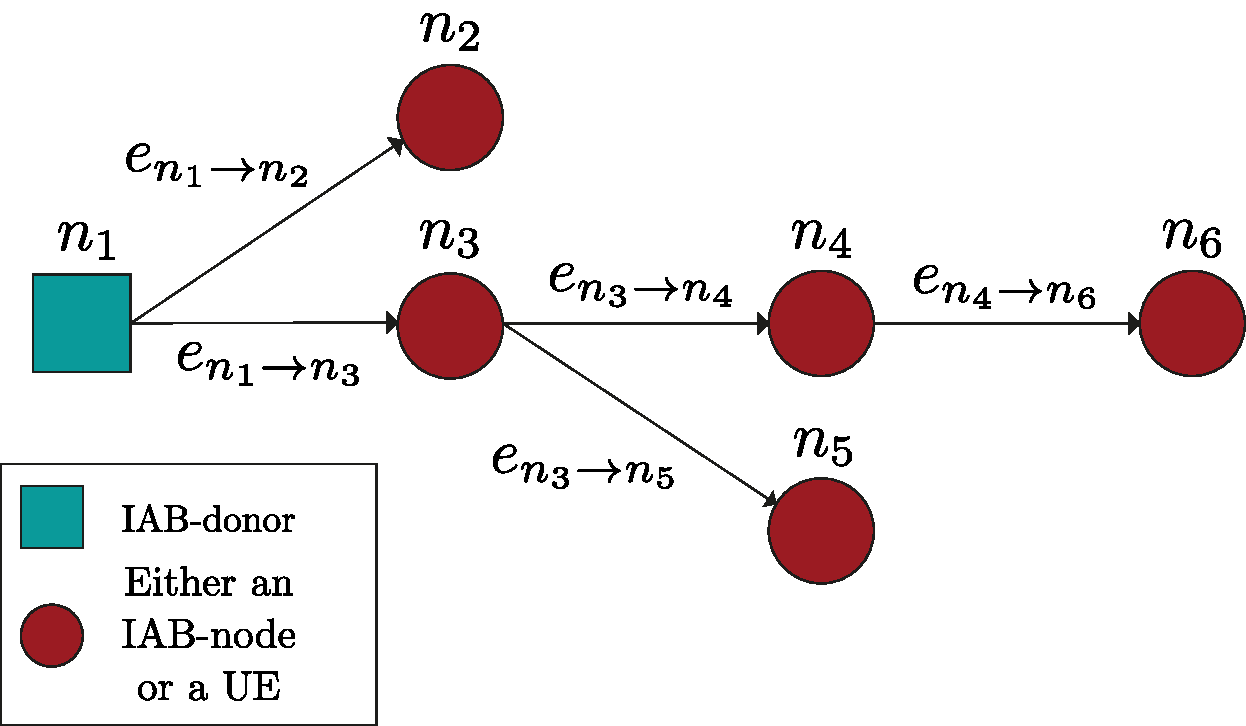
\includegraphics[width=0.55\columnwidth]{Figures/CentralResourceManagement/IAB_Notation.pdf}}
    \caption{Comparison of the \gls{iab} network topologies analyzed in~\cite{3gpp_38_874} and related notation.}
    \label{Fig:IAB_top_not}
    % \vspace{-.6cm}  
\end{figure}

\subsubsection{Network topology}
In general, an \gls{iab} network is a deployment where a percentage of \glspl{gnb} (i.e., the \gls{iab}-nodes) use wireless backhaul connections to connect to a few \glspl{gnb} (i.e., the \gls{iab}-donors) which feature a wired connection to the core network, as can be seen in Fig.~\ref{Fig:IAB_top_not}.
Moreover, these deployments exhibit a \textit{multi-hop} topology where a strict parent-child relation is present. The former can be represented by the \gls{iab}-donor itself or an \gls{iab}-node; the latter by either \gls{ue}s or downstream \gls{iab}-nodes. In~\cite{3gpp_38_874}, no a priori limit on the number of backhaul hops is introduced. As a consequence, \gls{3gpp} argues that \gls{iab} protocols should provide sufficient flexibility with respect to the number of backhaul hops. 
Moreover, the \gls{si} on \gls{iab}~\cite{3gpp_38_874} highlights the support for both the topologies depicted in Fig.~\ref{Fig:IAB_topology}, i.e., \gls{st} and \gls{dag} \gls{iab}. Clearly, the former exhibits less complexity but, at the same time, poses some limits in terms of network performance: the possible presence of obstacles may result in a service interruption, due to the unique backhaul route established by the \glspl{ue}. 
On the other hand, a \gls{dag} topology offers routing redundancy, which can be used not only to decrease the probability of experiencing a ``topological blockage," but also for load balancing purposes.

\subsubsection{Multiple access schemes and scheduling}
An in-band, dynamic partitioning of the access and backhaul spectrum resources is currently preferred by \gls{3gpp}~\cite{3gpp_38_874, 3gpp_38_174}, together with half-duplex operations of the \gls{iab}-nodes. Moreover, most of the literature suggests that \gls{5g} \gls{mmwave} systems will operate in a \gls{tdd} fashion~\cite{khan2011mmwave, dutta2017frame}. This choice is mainly driven by the stringent latency requirements which the next generation of mobile networks will be required to support, and by the usage of analog or hybrid beamforming. The usage of \gls{fdd}, in conjunction with the presence of large chunks of bandwidth, would lead to severe resource under-utilization and make channel estimation more difficult.
Based on these considerations, the system model exhibits a \gls{tdd}, \gls{tdma}-based scheduling where the access/backhaul interfaces are multiplexed in a half-duplex manner. 
Coupled with \glspl{mmwave} directionality, this means that self and inter-cell-interference are both limited, as reported by~\cite{qualcomm1}.
Furthermore, at any given time instant, each node of the \gls{iab} network cannot be simultaneously involved in more than one transmission or reception. In particular, \gls{iab}-nodes cannot schedule time and frequency resources which are already allocated by their parent for backhaul communications which involve them.
Moreover, the backhaul links of a given \gls{gnb} might also carry data which is destined to (and/or generated by) \glspl{ue} which are connected to different base stations. 
As a consequence, an \gls{iab}-network exhibits a marked and peculiar inter-dependence between the resource allocations of the various base stations, which is the major motivation for the introduction of a semi-centralized framework. 

Finally, the introduction of resource coordination mechanisms and related signaling is explicitly supported in the \gls{iab} specification drafts~\cite{3gpp_38_874, 3gpp_38_174}. Nevertheless, these solutions must reuse as much as possible the available NR specifications and
require at most minimal changes to the Rel.15 \gls{5gc} and \gls{nr}.


\subsubsection{System model}
\label{Subsec:sys_model}

According to these assumptions and referring to Fig.~\ref{Fig:IAB_notation}., a generic \gls{iab} network can be modeled as a directed graph $\mathcal{G} = \{\mathcal{N},  \mathcal{E} \}$, where the set of nodes $\mathcal{N} \mathop = \limits^{\Delta} \, \{ n_1, \, n_2, \, \ldots \, n_{\vert \mathcal{N} \vert }  \}$ comprises the \gls{iab}-donor, the various \gls{iab}-nodes and the \glspl{ue}. 
Accordingly, the set of directed edges $\mathcal{E} \mathop = \limits^{\Delta} \, \{ e_{1} , \, e_{2}, \, \ldots \, \allowbreak e_{\vert \mathcal{E} \vert} \} \equiv \{ e_{n_j \to n_k} \}_{j, k} $, where the edge $e_{n_j \to n_k}$ originates at the parent node $n_j$ and terminates at the children $n_k$, comprises in all the active cell attachments, either of mobile terminals to a \gls{gnb} or from \gls{iab}-nodes towards their parent node.
Since the goal of this section is to study backhaul/access resource partitioning policies, this generic model can be actually simplified: in fact, all the \glspl{ue} connected to a given \gls{gnb} can be represented by a single node in $\mathcal{G}$ without any loss of generality. Similarly, the same holds true for their links toward the serving \gls{gnb}, which can then be represented by a single edge. 
%TODO Maybe mention that as a consequence the number of edges is significantly reduced, taking into consideration the expected # of UEs connected to a BS in 5G systems
Furthermore, this work focuses on \gls{st} topologies only. 

We define as \textit{feasible schedule} any set of links $\mathcal{E'} \subseteq \mathcal{E}$ such that none of them share a common vertex, i.e., $ \forall \, e_{n_j \to n_k} \neq e_{n_l \to n_m} \in \mathcal{E'}$ it holds that $n_{j} \neq n_{m}$ and $n_{l} \neq n_{k}$. Let then $f_u$ be a utility \textit{additive map}, namely, a function such that the overall utility experienced by the system when scheduling edges $e_1$ and $e_2$ satisfies $f_u (e_1, e_2) = f_u (e_1) + f_u(e_2)$. Let also $\mathcal{W} \mathop = \limits^{\Delta} \, \{ w_1, \, w_2, \, \ldots \, w_{\vert \mathcal{E} \vert } \}$ be the set of positive weights whose generic entry $w_j$ represents the utility which is obtained when scheduling the $j$-th edge, namely, $w_j \mathop = \limits^{\Delta} \, f_u (e_j)$. Then, the overall utility of the system is $\mathcal{U} \mathop = \limits^{\Delta} \, \sum_{e_k \, \in \, \mathcal{E'}} f_u(e_k) = \sum_{e_k \, \in \, \mathcal{E'}} w_k $.
The goal is to find the feasible set $\mathcal{E'}^{*}$ which maximizes the overall utility, i.e., $\underset{\mathcal{E'}}{\mathrm{argmax}} \,\, \mathcal{U} $. In computer science, this task is typically referred to as the \textit{Maximum Weighted Matching} problem~\cite{Korte2002}.

Finding the \gls{mwm} of a given graph, in the general case, is not trivial from a computational point of view. 
In fact, the fastest known \gls{mwm} algorithm for generic graphs has a complexity of \bigO{\vert V \vert \vert E \vert + \vert V \vert^2 \log{\vert V \vert}}~\cite{1990Gabow}, posing serious limitations to the suitability of such algorithm to \gls{5g} and beyond networks, which target a connection density of 1 million devices per km\textsuperscript{2}. However, we argue that under the aforementioned assumptions on the system model, which restrict the network to an \gls{st} topology, it is possible to design an \gls{mwm}-based semi-centralized resource partitioning framework which exhibits linear complexity with respect to the network size and which, as a result, is able to satisfy the scalability requirements highlighted by \gls{3gpp} in~\cite{3gpp_38_874}. 
Nevertheless, the proposed framework can be easily extended to the case of a \gls{dag} \gls{iab} network. In such regard, a sub-optimal strategy is to periodically discard, during each centralized allocation, the redundant edges of each node. In such a way, the input which is fed to the \texttt{T-MWM} algorithm is, effectively, an \gls{st}. A second, optimal extension can be obtained by computing at the controller the \gls{mwm} of the network via a generic \gls{mwm} algorithm, instead of using the \gls{st}-specific \texttt{T-MWM} as in the proposed framework. However, this strategy would feature a higher computational complexity.

\subsection{Semi-centralized resource allocation scheme for IAB networks}
\label{Sec:scheme_main}

This section presents an \gls{mwm} algorithm for \gls{st} topologies (Section~\ref{Sec:T-MWM}), an efficient and \gls{mwm}-based semi-centralized resource partitioning framework for \gls{iab} networks (Section~\ref{Sec:Cent-scheme}) and some considerations about its implementation (Section~\ref{Sec:ns3-impl}). 
Specifically, the proposed scheme collects at a controller installed on the \gls{iab}-donor L1 and/or L3 measurements from the various \glspl{gnb}. Then, it uses such information to build a weighted \gls{st} which represents the \gls{iab}-network. In particular, the network topology is inferred by examining the incoming parent-child associations. The edge weights are also computed from the received measurements, based on the specific policy (hence, of target \glspl{kpi}) of choice. Finally, the resource partitioning is optimized by computing an \gls{mwm} of the network and then prioritizing the links which comprise it. A high level diagram of is provided in Fig.~\ref{Fig:Diagram}.

\begin{figure}[t!]
    \centering
    \subfloat[IAB protocol stack and topology.\label{Fig:IAB-net}]{
    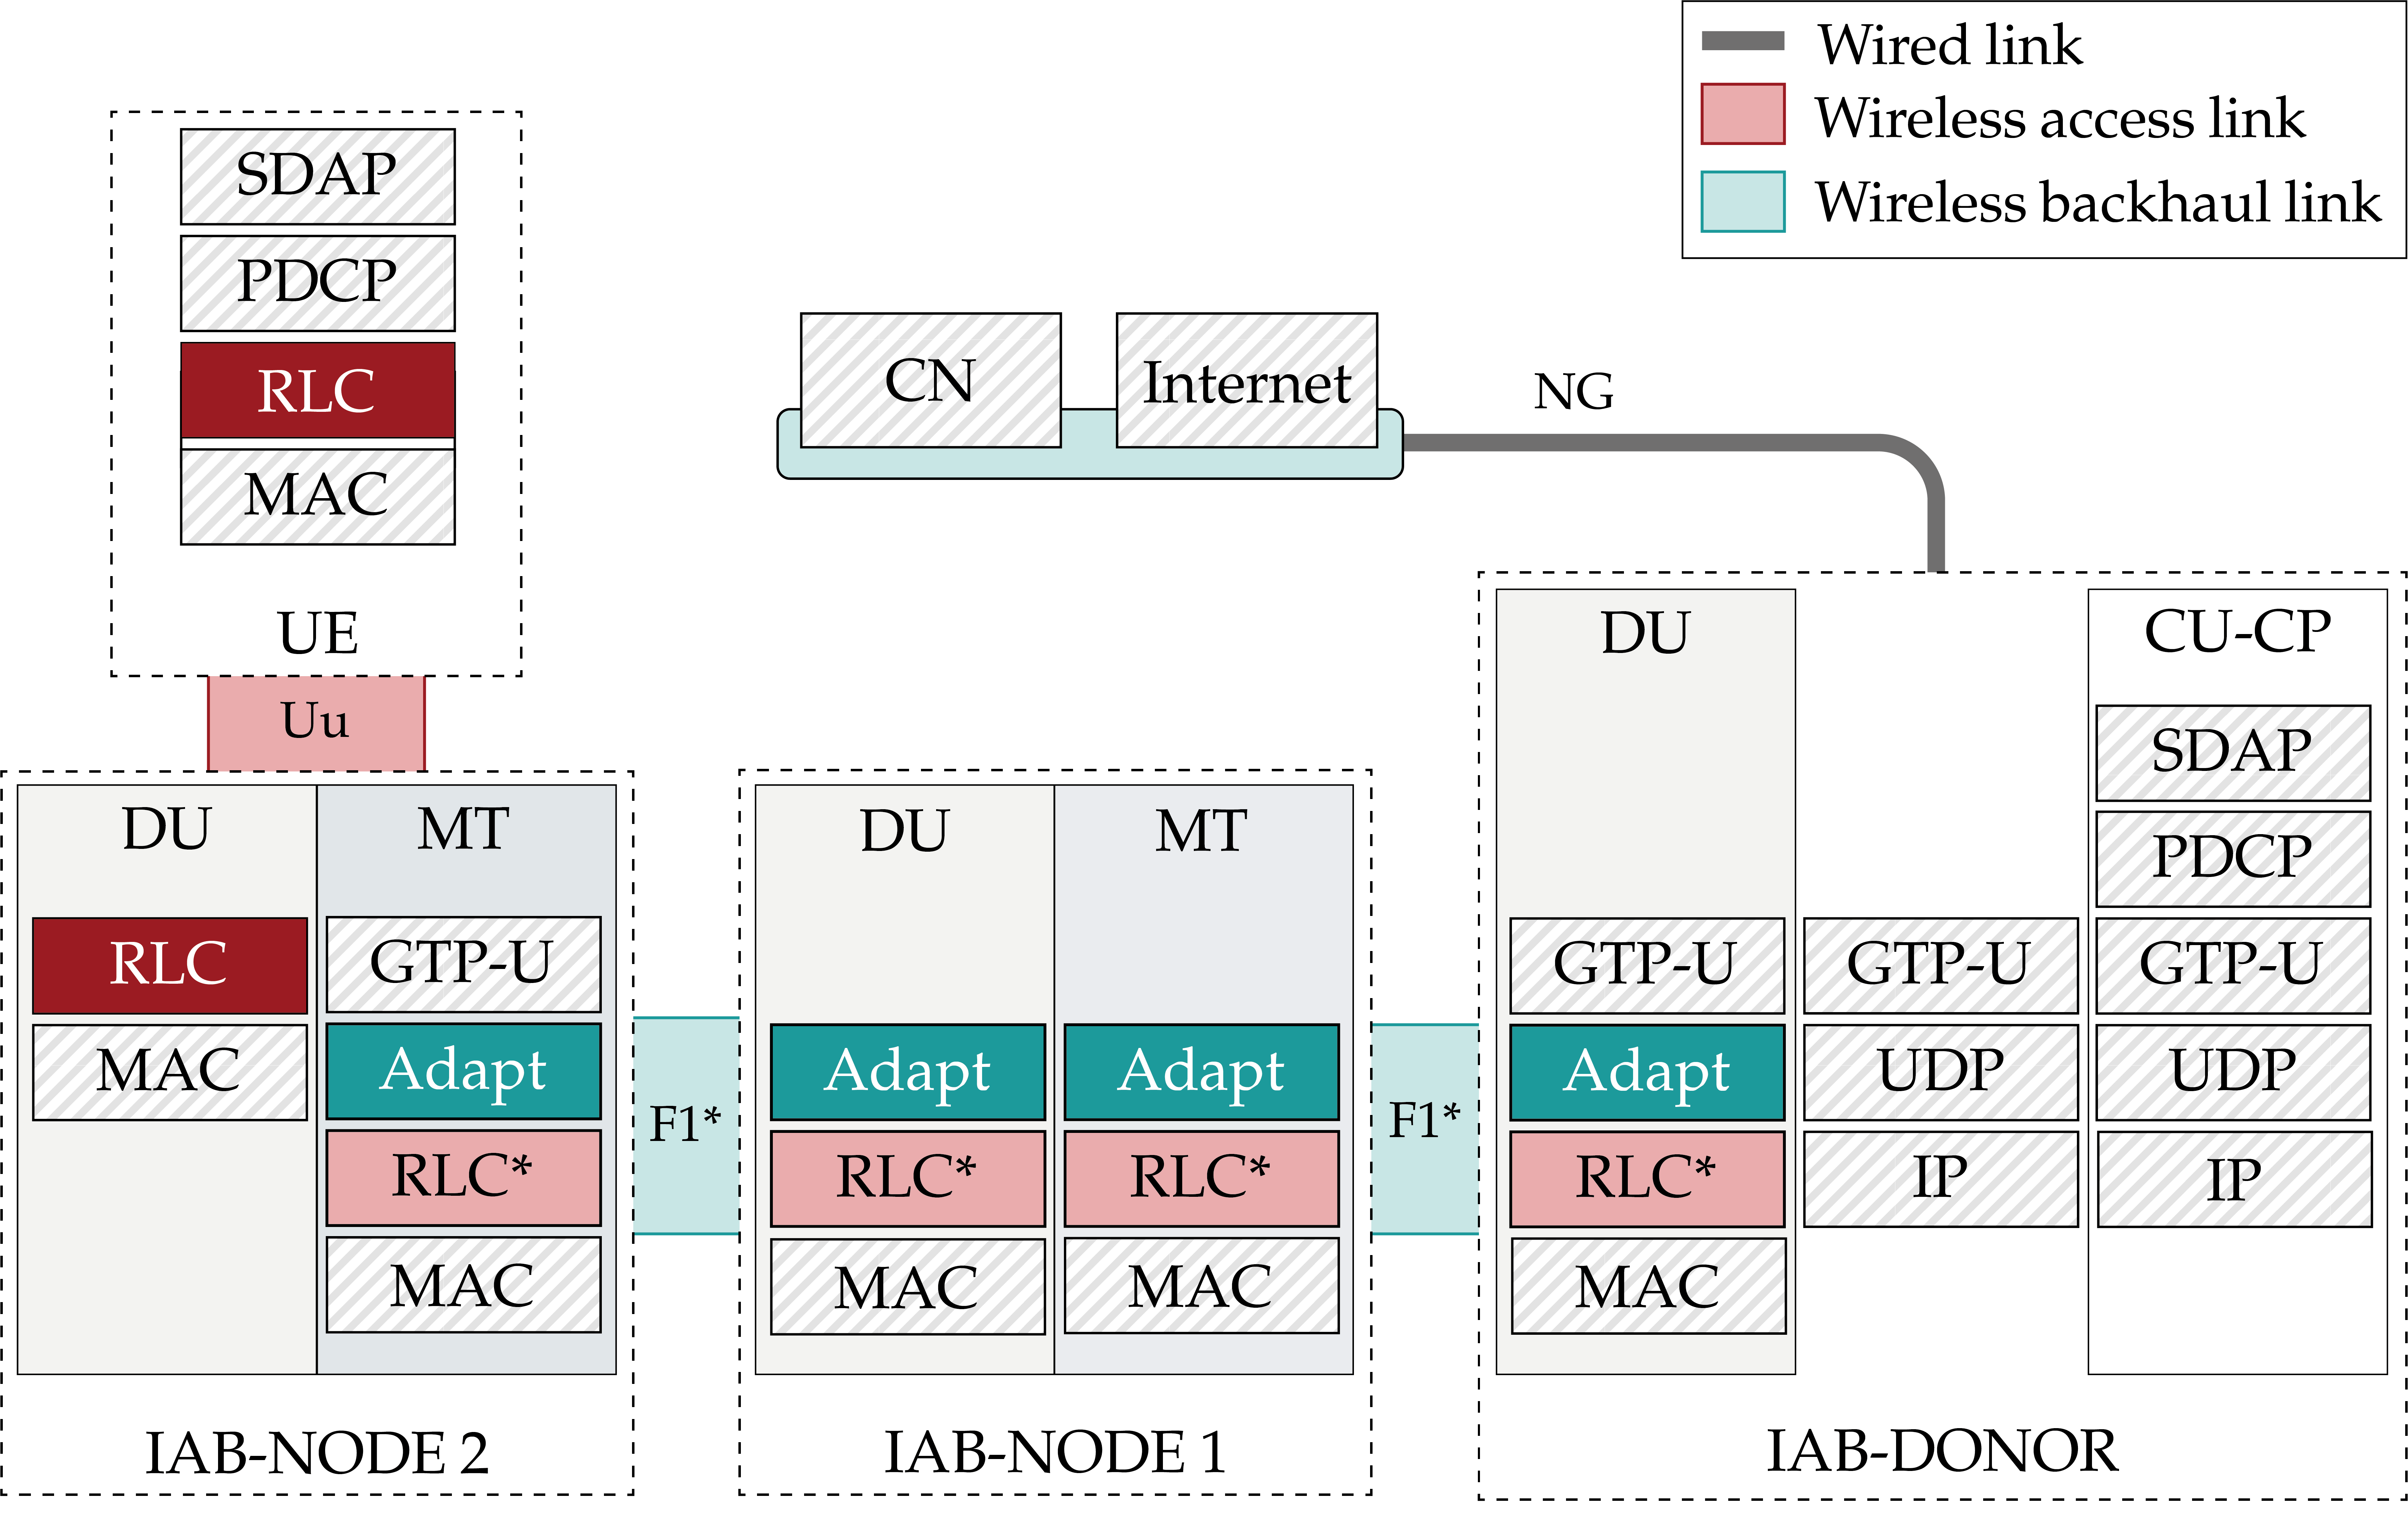
\includegraphics[width=0.88\linewidth]{Figures/CentralResourceManagement/architecture_full.png}}\hfill
    \centering
    \subfloat[High level diagram of the proposed \gls{mwm}-based framework.\label{Fig:Diagram}]{
    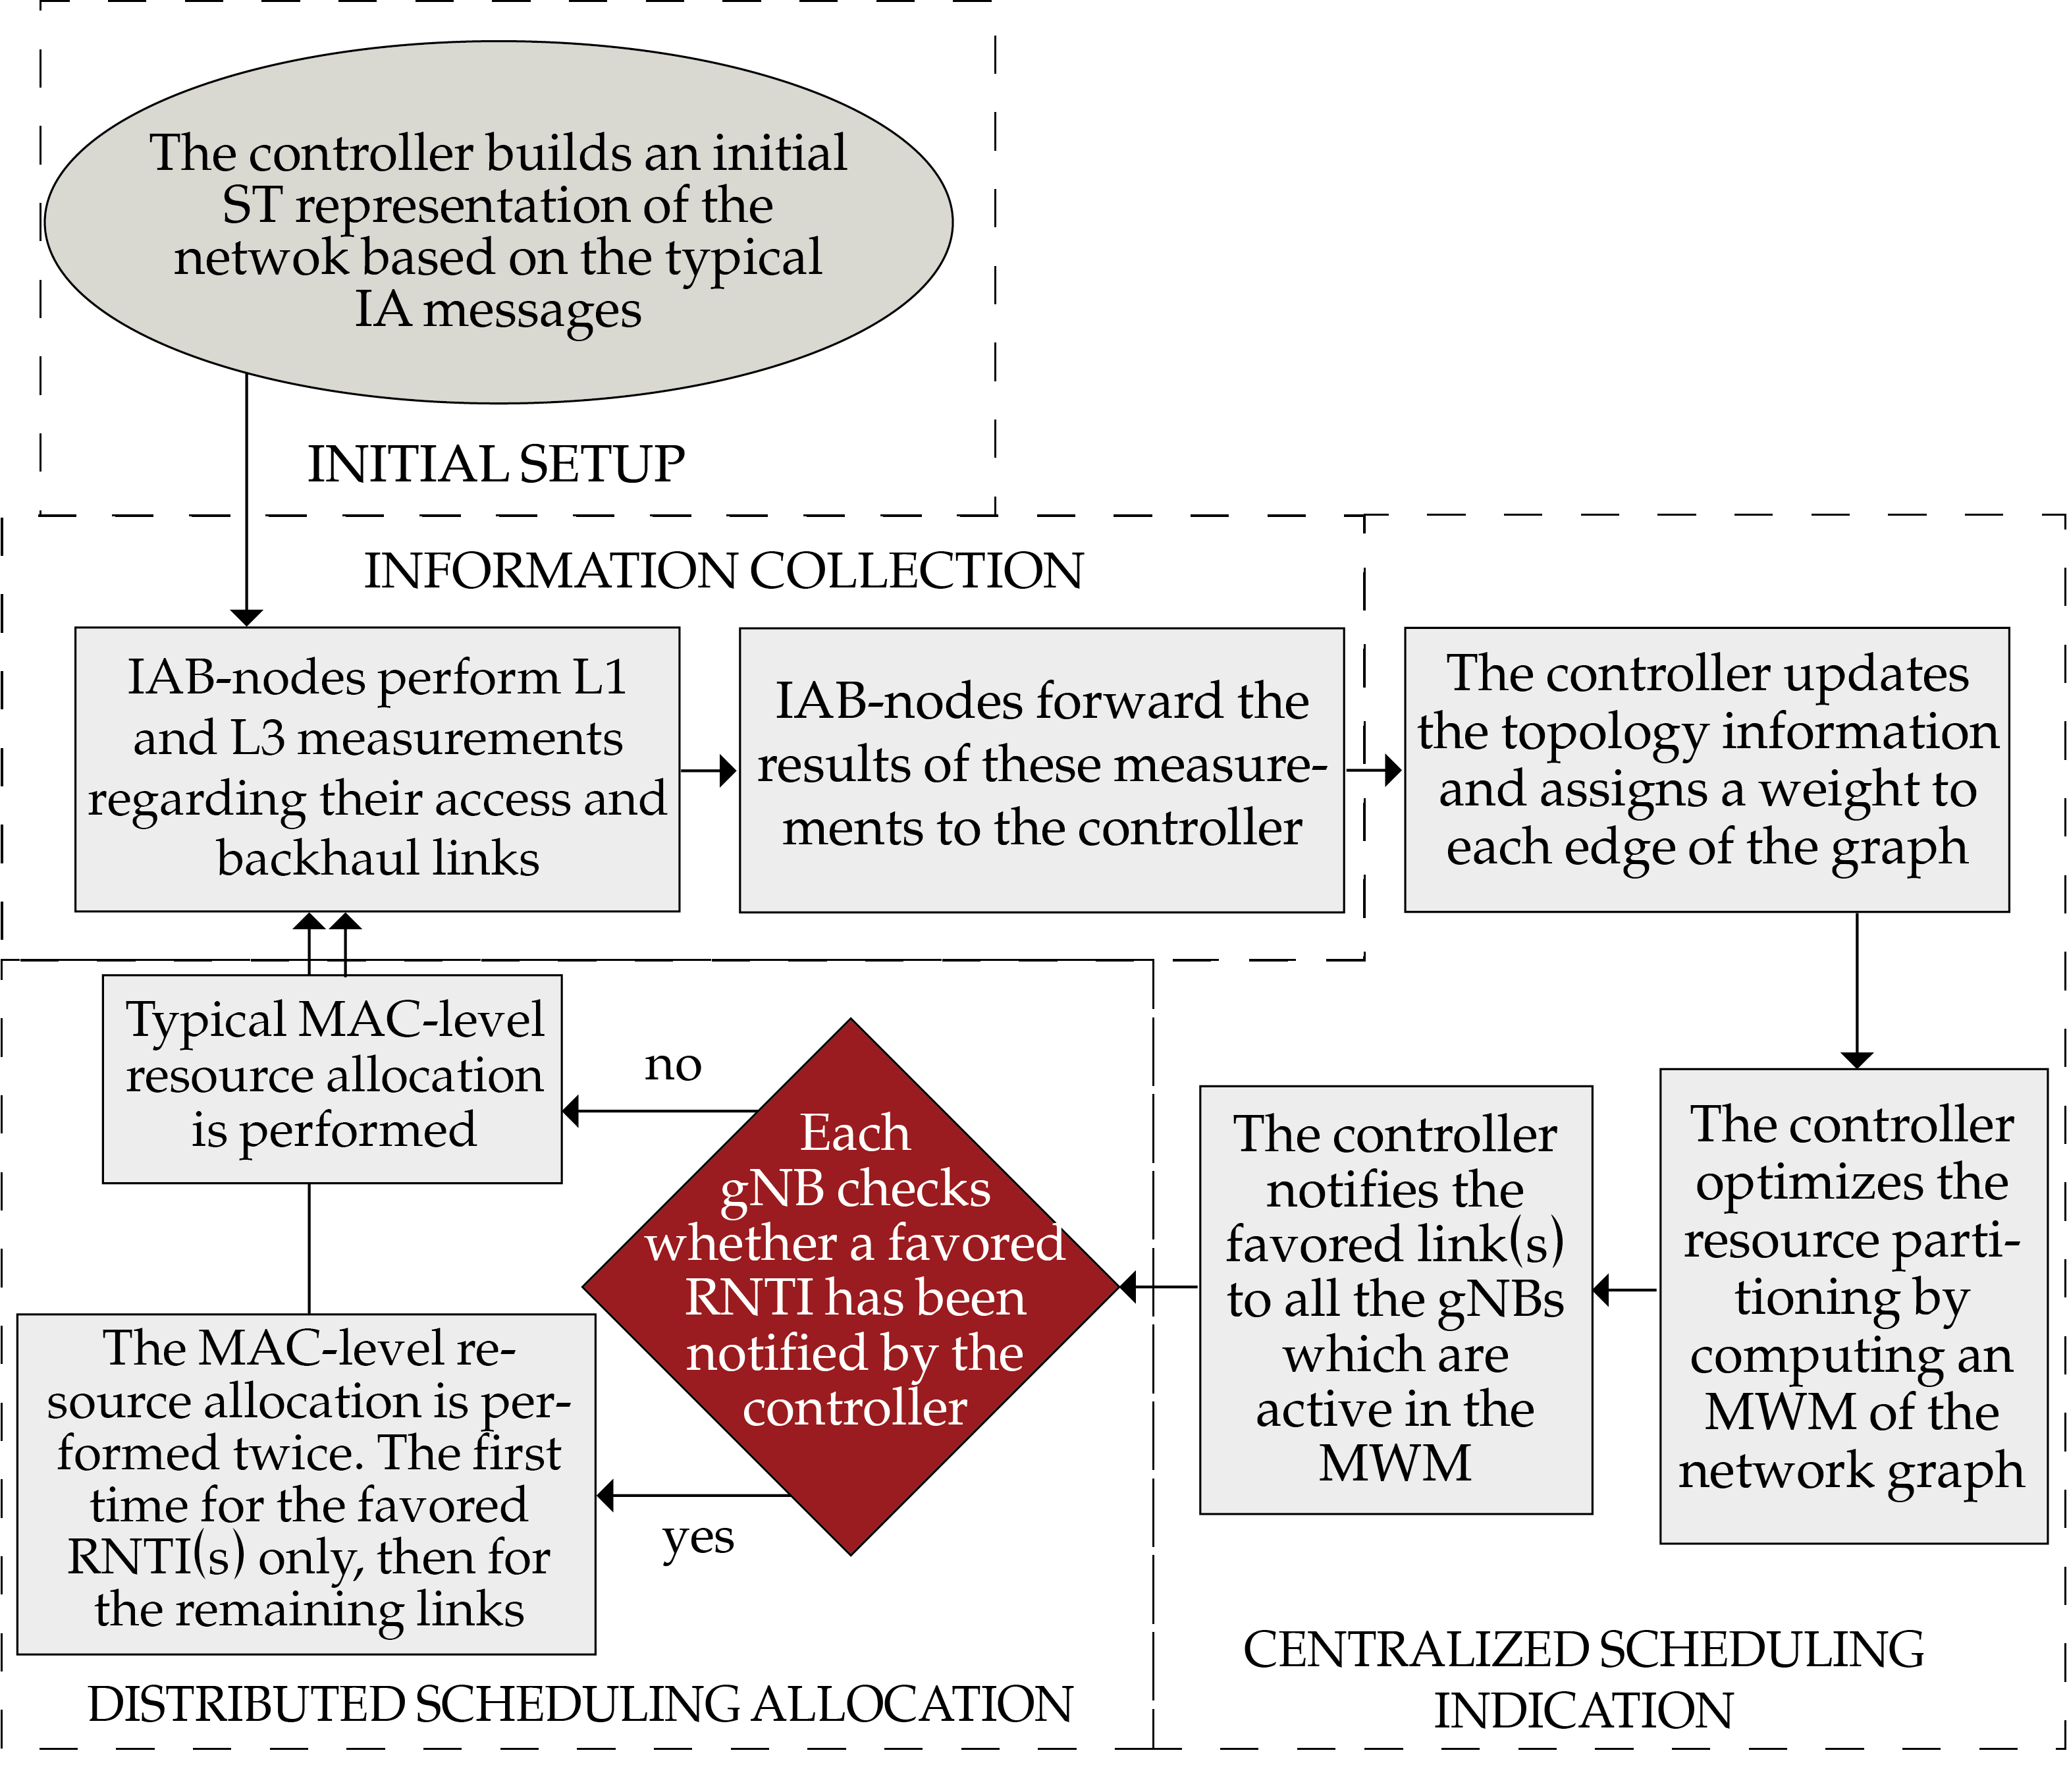
\includegraphics[width=0.88\linewidth]{Figures/CentralResourceManagement/FlowChart_IAB.png}}
    \caption{IAB topology and proposed MWM-based framework.}
    \label{fig:fr-top}
\end{figure}

\subsubsection{MWM for ST graphs}
\label{Sec:T-MWM}

As the first of our contributions, we present an algorithm, hereby called \texttt{T-MWM}, which computes the \gls{mwm} of an \gls{st} in linear time. In particular, \texttt{T-MWM} is a bottom-up algorithm which, upon receiving as input a weighted \gls{st} $\mathcal{G}$ described by its edge map $\mathbf{E}$ and the corresponding weight map $\mathbf{W}$, produces as output a set of active edges $\mathbf{E^*}$ which are an \gls{mwm} of $\mathcal{G}$. That is to say, $\mathbf{E^*}$ is a matching of $\mathcal{G}$ which yields the globally maximum utility.
Furthermore, $\mathbf{E}$ is from now on assumed to exhibit the following invariant: each \gls{iab} parent precedes its children in the map, hence avoiding the need for a recursion. 
This is automatically obtained as each \gls{iab} child connects after its parent, and is thus added to the map in a subsequent position.
Nevertheless, this assumption can be easily relaxed, albeit at the cost of losing as a side-effect the bottom-up design.


The proposed algorithm is designed starting from the observation that, given the generic node $n_k \in \mathcal{G}$ and a matching $\mathbf{\bar{E}}$ of $\mathcal{G}$, we can identify the following mutually exclusive and collectively exhaustive cases: $\mathbf{\bar{E}}$ can contain either one or zero edges which originate from $n_k$. Based on this fact, we then discern the optimal utilities which can be obtained in each of these cases. Specifically, we define the maximum utilities yielded by a matching of $n_k$'s sub-tree which either contains a link originating from $n_k$ or not as $\mathbf{F}(n_k)$ and $\mathbf{G}(n_k)$, respectively.
Then, as can be seen in Alg.~\ref{Alg:tmwm}, the \texttt{T-MWM} algorithm basically consists in two traversals of the network graph. During the first one we compute the $\mathbf{G}$ and $\mathbf{F}$ functions for all the nodes in $\mathcal{G}$ using the recursive formulas provided by Lemma~\ref{lemma_utils}. Finally, during the second traversal, this knowledge is used for computing an \gls{mwm} of the network; the correctness of this last phase is proved by Lemma~\ref{lemma_active_edges}.

\begin{algorithm}[tbp!]
\footnotesize
    \caption{Tree-Maximum Weighted Matching}
    \label{Alg:tmwm}
    \hspace*{\algorithmicindent} \textbf{Input:} A weighted \gls{st} $\mathcal{G}$ encoded by a map $\mathbf{E}$, which associates each node in $\mathcal{G}$ to its edges, and the corresponding weights map $\mathbf{W}$. \\ 
    \hspace*{\algorithmicindent} \textbf{Output:} An \gls{mwm} $\mathbf{E^*}$ of $\mathcal{G}$. 
    \begin{algorithmic}[1] % The number tells where the line numbering should start
        \Procedure{\texttt{T-MWM}}{$\mathbf{E}, \mathbf{W}$} 
            \State $\mathbf{F} \gets \mathbf{0}$; $\mathbf{G} \gets \mathbf{0}$ \Comment{Initialize the utility vectors to zero vectors}
            \State $\mathbf{E^*} \gets \{ \}$ \Comment{Initialize the set of active edges as empty}
            \For{each internal node $n_k \in \mathbf{E}$} \Comment{\parbox[t]{.43\linewidth}{In ascending order w.r.t. to their depth in $\mathcal{G}$}}
            \State $maxUtil \gets - \infty$;  $\mathbf{maxUtilChild}(n_k) \gets \{ \}$
            \For{each edge $e_{n_k \to n_j} \in \mathbf{E}(n_k) $} \Comment{Iterate over its edges}
                \State $\mathbf{G}(n_k) \gets \mathbf{G}(n_k) + \max \left\{ \mathbf{F}(n_j), \mathbf{G}(n_j) \right\}$
                \State $currUtil \gets \mathbf{W} ( e_{n_k \to n_j} ) - \left[ \mathbf{F}(n_j) - \mathbf{G}(n_j) \right]^+  $
            \If{$currUtil > maxUtil$}
            	\State $maxUtil \gets currUtil$;  $\mathbf{maxUtilChild}(n_k) \gets n_j$ 
            \EndIf
            \EndFor\label{edgesFor}
            \State $\mathbf{F}(n_k) \gets \mathbf{G}(n_k) + maxUtil$ 
            \EndFor\label{nodesFor}
			
			\For{each internal node $n_k \in \mathbf{E}$} \Comment{\parbox[t]{.43\linewidth}{In ascending order w.r.t. to their depth in $\mathcal{G}$}}			
			
				\If { $\mathbf{F}(n_k) \geq \mathbf{G}(n_k)$}
					\State $\mathbf{E^*} \gets \mathbf{E^*} \cup e_{n_k \to \mathbf{maxUtilChild}(n_k)}$
					\State $\mathbf{F}(\mathbf{maxUtilChild}(n_k)) \gets -\infty$ \Comment{\parbox[t]{.3\linewidth}{Ensure child does not get activated multiple times}}
				\EndIf\label{activeIf}
			\EndFor\label{edgesFor2}            
            
            \State \textbf{return} $\mathbf{E^*}$
        \EndProcedure
    \end{algorithmic}
\end{algorithm}

\begin{lem}
\label{lemma_utils}
Given an \gls{st} $\mathcal{G}$, consider its generic internal node $n_k$. Let then $\mathbf{F}(n_k)$ be the maximum utility yielded by a matching of $n_k$'s sub-tree which activates a link originating from $n_k$, and $\mathbf{G}(n_k)$, conversely, the utility provided when such matching contains no links which feature $n_k$ as parent. Then, we have that:
\[ 
\begin{cases}
\mathbf{G}(n_k) = \sum\limits_{ \{ n_j \}_k} \max \left\{ \mathbf{F}(n_j), \mathbf{G}(n_j) \right\} \\

\begin{aligned}
\mathbf{F}(n_k) &= \mathbf{G}(n_k) + \underset{\{ n_j \}_k }{\max} \{ \mathbf{W} ( e_{n_k \to n_j} ) \\
&- \left[ \mathbf{F}(n_j) - \mathbf{G}(n_j) \right]^+ \}
\end{aligned}


\end{cases}
\]
where the set $\{ n_j \}_k$ comprises all the children of $n_k$ and $\left[ x \right]^+ = \max\{x, 0\}$ is the positive part of $x$.
%
Conversely, for leaf nodes $n_l$ it holds that $\mathbf{F}(n_l) \equiv \mathbf{G}(n_l) \equiv 0 $.
\end{lem}

\begin{proof}
This lemma can be proved by induction over the height $h_k$ of the sub-tree corresponding to node $n_k$. The base case is $h_k = 0$, i.e., when $n_k$ is a leaf node; in this case, trivially, both $\mathbf{F}(n_k)$ and $\mathbf{G}(n_k)$ are zero since no links exhibit $n_k$ as parent node and the sub-tree of $\mathcal{G}$ which originates in $n_k$ consists of $n_k$ only, respectively.

Then, assume that $n_k$'s sub-tree exhibits a generic height $h_k > 0$, and that the above formulas hold for each of its children sub-trees, which exhibit a height $h_j < h_k$. If we do not activate any edge which originates from $n_k$, then no added constraints are introduced concerning the edges which can be activated in its children sub-trees. Therefore, %the maximum utility achieved by any matching of $n_k$'s sub-tree, without activating any node which originates from $n_k$, 
$\mathbf{G}(n_k)$ is simply the sum of the utilities achieved by any \gls{mwm} computed on its children sub-trees, i.e.,  $\mathbf{G}(n_k) = \sum\limits_{ \{ n_j \}_k} \max \left\{ \mathbf{F}(n_j), \mathbf{G}(n_j) \right\}$.
The remaining option is to activate exactly one edge, hereby called $e_{n_k \to n_m}$, which originates from $n_k$. In this case, no additional edges which feature $n_m$ as parent can be added to the matching. As a consequence, the contribution of $n_m$'s sub-tree on $\mathbf{F}(n_k)$ reads $\mathbf{G}(n_m)$. Conversely, no additional constraints are introduced regarding the other nodes. It follows that the utility obtained in this instance reads:
\[ \sum_{ \{ n_j \neq n_m\}_k } \max \left\{ \mathbf{F}(n_j), \mathbf{G}(n_j) \right\} +  \mathbf{W} ( e_{n_k \to n_m} ) + \mathbf{G}(n_m) \]
and can be rewritten as:
\[  \mathbf{G}(n_k) + \mathbf{W} ( e_{n_k \to n_m} ) - \left[ \mathbf{F}(n_m) - \mathbf{G}(n_m) \right]^+ \]
Finally, such utility is clearly maximized when $n_m$ is chosen as $ \underset{ \{ n_j \}_k }{\mathrm{argmax}} \, \{ \mathbf{W} ( e_{n_k \to n_j} ) - \left[ \mathbf{F}(n_j) - \mathbf{G}(n_j) \right]^+ \}$, yielding:
\[ \mathbf{F}(n_k) = \mathbf{G}(n_k) + \underset{\{ n_j \}_k }{\max} \, \{ \mathbf{W} ( e_{n_k \to n_j} ) - \left[ \mathbf{F}(n_j) -  \mathbf{G}(n_j) \right]^+ \} \qedhere \] 
\end{proof}

\begin{lem}
\label{lemma_active_edges}
Given an \gls{st} $\mathcal{G}$ of root $n_r$ and the $\mathbf{F}$ and $\mathbf{G}$ functions computed as per Lemma~\ref{lemma_utils}, an \gls{mwm} $\mathbf{E^*}$ of $\mathcal{G}$ can be computed by performing the following procedure:
%, in a recursive fashion
\begin{enumerate}
\item If $ \, \mathbf{F}(n_r) \geq \mathbf{G}(n_r) $, add to $\mathbf{E^*}$ the edge from $n_r$ to $n_m$, where the latter is defined as $n_m \mathop = \limits^{\Delta} \, \underset{ \{ n_j \}_r }{\mathrm{argmax}} \, \{ \mathbf{W} ( e_{n_r \to n_j} ) - \left[ \mathbf{F}(n_j) - \mathbf{G}(n_j) \right]^+ \}$. Then, repeat recursively on all the sub-trees corresponding to $n_r$'s children $\{ n_j\}_r \, \vert \, n_j \neq n_m$ and on the children of $n_m$ itself.
\item If $ \, \mathbf{F}(n_r) < \mathbf{G}(n_r) $, repeat recursively on all the sub-trees corresponding to $n_r$'s children.
\end{enumerate}
\end{lem}

\begin{proof}
The above procedure always yields a feasible activation, i.e., a matching of $\mathcal{G}$.  In particular, in either options we never recurse on a node which has already been activated, hence no pair of edges $\in \mathbf{E^*}$ can share any vertices. Furthermore, due to the properties of $\mathbf{F}$ and $\mathbf{G}$, whenever $\mathbf{F}(n_r) \geq \mathbf{G}(n_r)$ a matching yielding maximal utility can be obtained by activating the edge $e_{ n_r \to n_m }$, where $n_m \mathop = \limits^{\Delta} \, \underset{ \{ n_j \}_r }{\mathrm{argmax}} \, \{ \mathbf{W} ( e_{n_r \to n_j} ) - \left[ \mathbf{F}(n_j) - \mathbf{G}(n_j) \right]^+ \}$.
Since the procedure is then recursively repeated on $n_r$'s children and the validity of $\mathbf{F}$ and $\mathbf{G}$ properties holds for each sub-tree in $\mathcal{G}$, the set of edges $\mathbf{E^*}$ produced by the above procedure comprise a \textit{maximal} matching, i.e., they yield the maximum possible utility among all the feasible schedules. 
\end{proof}

Regarding the computational complexity of the proposed algorithm, it can be observed that during the first phase the main loop effectively scans each edge of $\mathcal{G}$, hence exhibiting a complexity \bigO{\vert \mathbf{E} \vert}. Moreover,
the second phase of \texttt{T-MWM} has complexity \bigO{\vert \mathbf{V} \vert}, since it loops through all the network nodes.
Therefore, we can conclude that the overall asymptotic complexity of the algorithm is \bigO{\vert \mathbf{V} \vert + \vert \mathbf{E} \vert}, or, equivalently, \bigO{\vert \mathbf{V} \vert} since in an \gls{st} the number of edges equals $\vert \mathbf{V} \vert - 1$.

\subsection{Semi-centralized resource partitioning scheme}
\label{Sec:Cent-scheme}
Based on the system model introduced in Section~\ref{Sec:Sys-model}, and the \texttt{T-MWM} algorithm, we present a generic optimization framework which partially centralizes the backhaul/access resource partitioning process, in compliance with the guidelines of~\cite{3gpp_38_874}. 
The goal of this framework is to aid the distributed schedulers, adapting the number of \gls{ofdm} symbols allocated to the backhaul and access interfaces to the phenomena which exhibit a sufficiently slow evolution over time, i.e., large scale fading and local congestion. % Maybe mention also effectiveness of centralized is exarcebated by TDD constraints
This optimization is undertaken with respect to a generic additive utility function $f_u$. An \gls{iab} network of arbitrary size is considered, composed of a single \gls{iab}-donor, multiple \gls{iab}-nodes and a (possibly time-varying) number of \glspl{ue} which connect to both types of \glspl{gnb}.
Furthermore, %let the topology of the \gls{iab} network be pre-computed, for instance by using the policies of~\cite{polese2018iab}, and 
assume that a central controller is installed on the \gls{iab}-donor. 

The proposed framework can be subdivided into the following phases, which are periodically repeated every $T_{alloc}$ subframes:
\begin{enumerate}
\item \label{Enum_frameword:item_one} \textbf{Initial setup}. This step, which is depicted in Fig.~\ref{Fig:Phase0}, consists in the computation of the simplified \gls{iab} network graph $\mathcal{G} \equiv \{ \mathcal{V}, \mathcal{E} \}$. Specifically, after this phase $\mathcal{V}$ comprises the donor and the various \gls{iab}-nodes. Accordingly, $\mathcal{E}$ contains their active cell associations.

\item \label{Enum_frameword:item_two} \textbf{Information collection}. During this phase, the various \gls{iab}-nodes send to the central controller a pre-established set of information for each of their children in $\mathcal{G}$. For instance, this feedback may consist in their congestion status and/or  information regarding their channel quality. To such end, the implementation presented in this section uses modified versions of pre-existing \gls{nr} Release 16 \glspl{ce}, as strongly recommended in the \gls{iab} SI~\cite{3gpp_38_874}. However, the scheme does not actually impose any limitations in such regard.
\item \label{Enum_frameword:item_three} \textbf{Centralized scheduling indication}. Upon reception of the feedback information, the central controller updates $\mathcal{G}$ by inspecting the received node-parent associations. Then, the set of weights $\mathcal{W}$ is calculated and an \gls{mwm} of $\mathcal{G}$ is computed, using the \texttt{T-MWM} algorithm. The output of this procedure is the activation set $\mathbf{E^*}$, which yields a globally optimum solution with respect to the chosen utility function. Subsequently, $\mathbf{E^*}$ is used as to create a set of \textit{favored} downstream nodes, i.e., of children which will be served with the highest priority by their parent, as depicted in Fig.~\ref{Fig:Phase2}. Finally, these scheduling indications are forwarded to the various \gls{iab}-nodes which act as parents in the edges of $\mathbf{E^*}$.

\begin{figure}[t!]
	\centering
  	\subfloat[The original topology, exhibiting the actual cell attachments, is depicted on the left. Conversely, the reduced one is shown on the right.\label{Fig:Phase0}]{
  	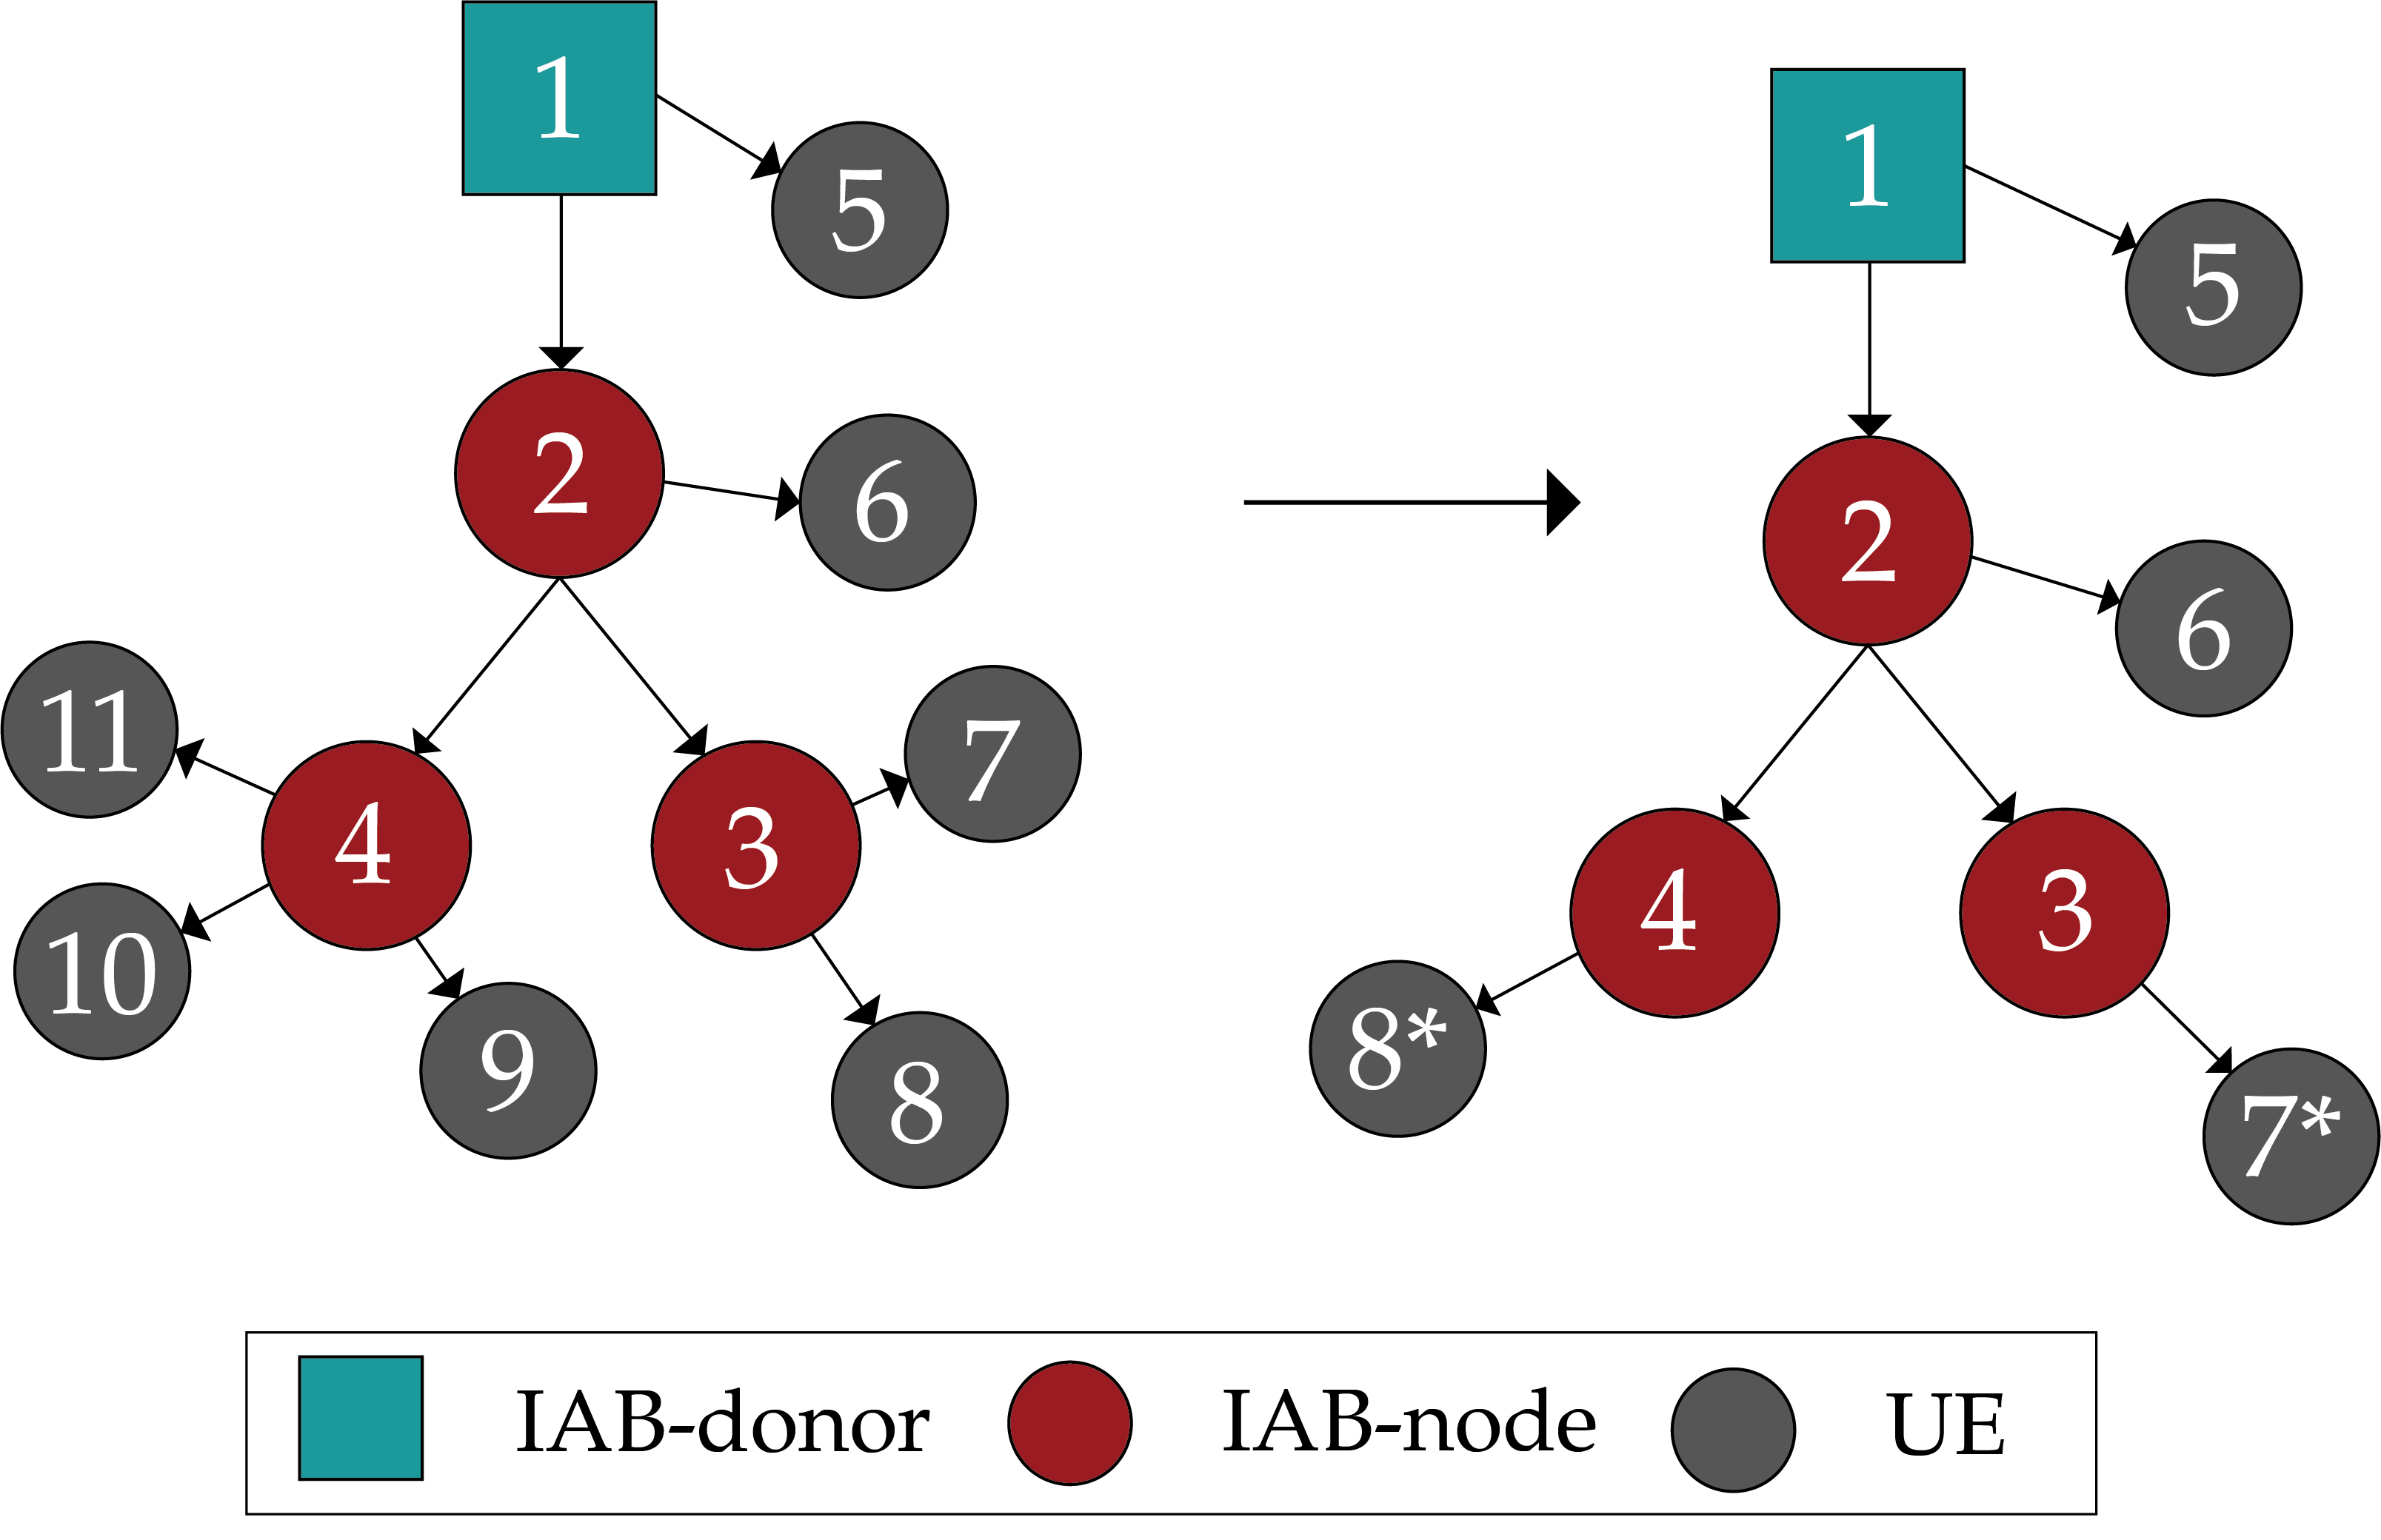
\includegraphics[width=0.65\linewidth]{Figures/CentralResourceManagement/Phase0.png}
    }\hfill
  	\subfloat[Computation of the \gls{mwm} and of the corresponding scheduling indications.\label{Fig:Phase2}]{
  	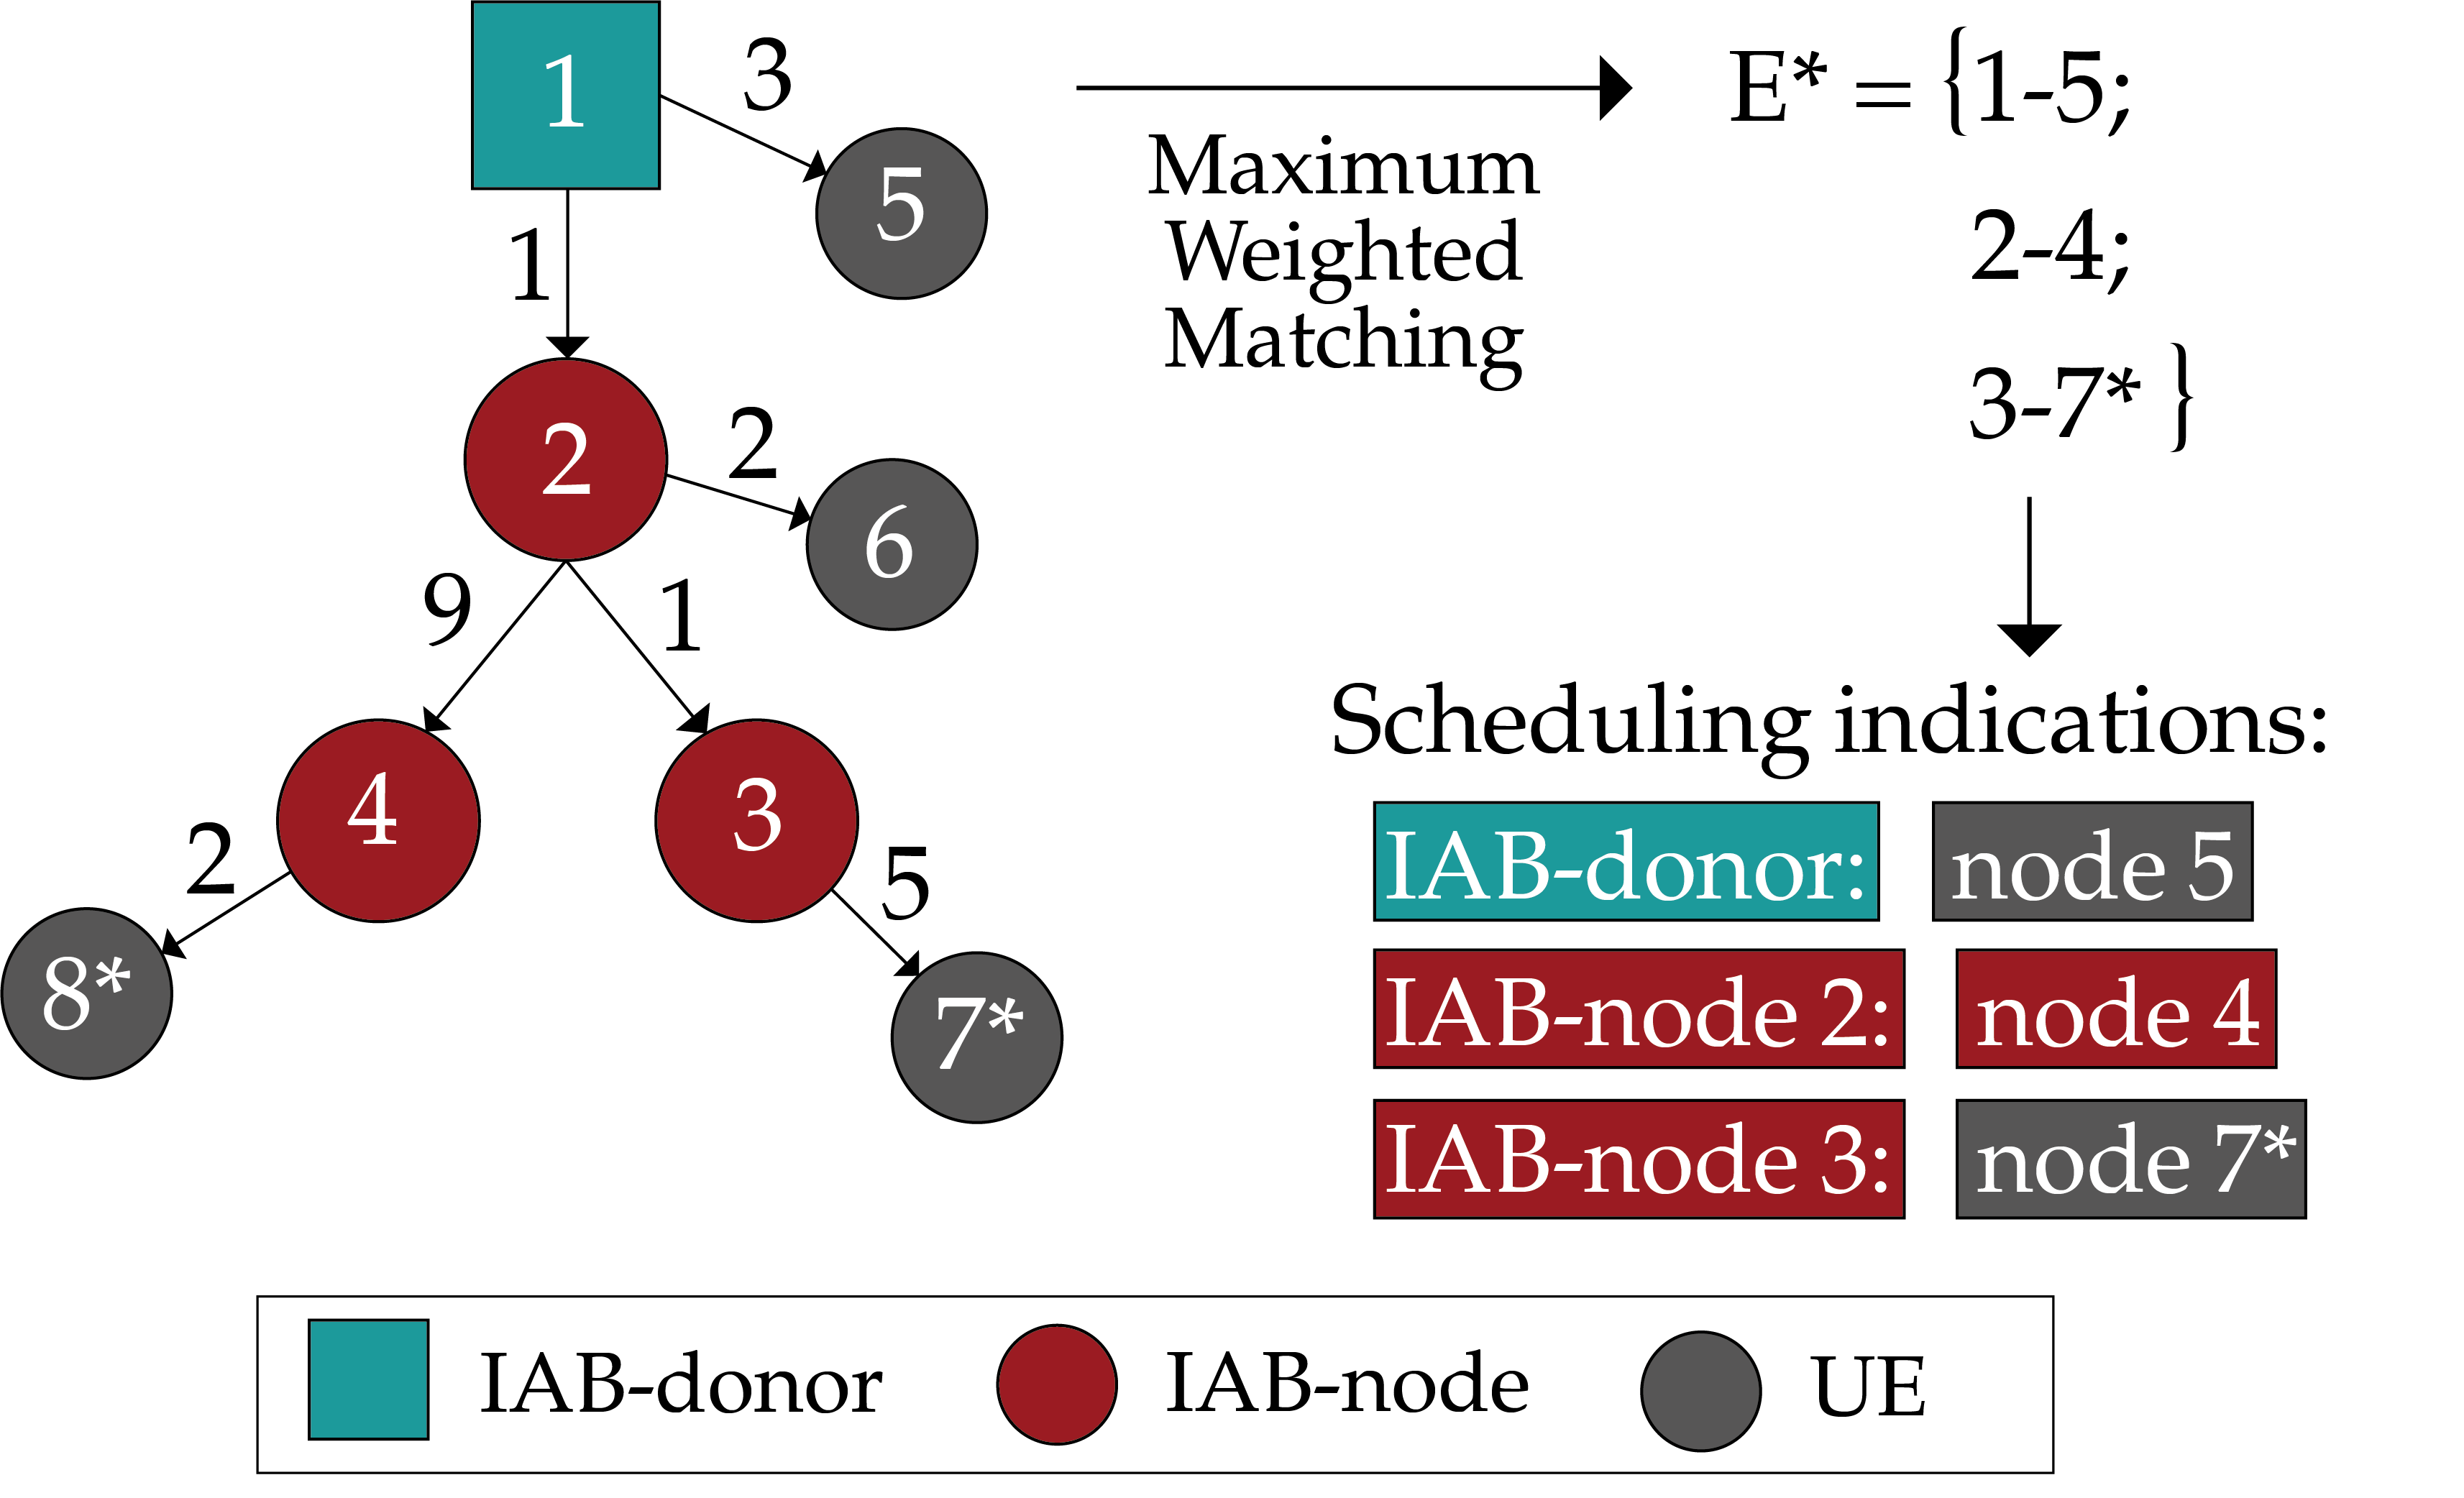
\includegraphics[width=0.65\linewidth]{Figures/CentralResourceManagement/Phase2.png}
    }
    \caption{High level scheme of the initial setup and centralized scheduling indication phases.}
    \label{Fig:Phases}
\end{figure}


\item \textbf{Distributed scheduling allocation}. During this phase, the various \gls{iab}-nodes make use of the indications received by the central controller, if available, in order to perform the actual scheduling (which is, therefore, predominantly distributed). Specifically, the favored nodes are served with the highest priority, while the remaining downstream nodes are scheduled if and only if the resource allocation of the former does not exhaust the available \gls{ofdm} symbols.
\end{enumerate}
It is important to note that since $\mathcal{G}$ contains only the \gls{iab}-nodes, the donor and at most one ``representative" \gls{ue} per \gls{gnb}, the proposed scheme effectively performs only the backhaul/access resource partitioning in a centralized manner. On the other hand, the actual \gls{mac}-level scheduling is still undertaken in a distributed fashion, albeit leveraging the indications produced by the central controller. The major advantages which this two-tier design exhibits, compared to a completely centralized solution, are the presence of a relatively light signaling overhead and the ability to promptly react to fast channel variations, for instance caused by small scale fading.  

\subsection{Implementation of semi-centralized allocation schemes in mmWave IAB networks}
\label{Sec:ns3-impl}

The remainder of this section discusses how the proposed scheme can be implemented in \gls{iab} deployments, with references to how the \gls{3gpp} specifications can support it. Moreover, an in-depth analysis of the framework's communication overhead and computational complexity is provided. To such end, let $\mathcal{G} = \{ V, E \}$ be the reduced network graph, computed as per Section~II-C, and, conversely, let $\mathcal{\bar{G}} = \{ \bar{V}, \bar{E} \}$ comprise all the nodes in the \gls{iab} network.
% presents an implementation of the proposed scheme in the network simulator ns-3, along with considerations on its implementation in real world deployments.

In general, the resource allocation framework requires (i) a central controller, which is installed on the \gls{iab}-donor, or could be deployed in a \gls{ric} following the O-RAN architecture~\cite{bonati2020open}; and (ii) a scheduler which exchanges resource coordination information with the former. %and computes the weights for the resource allocation.
In particular, and referring to the aforementioned phases of the proposed scheme, the following %communication overhead, computational complexity and implementation  
additional considerations can be made. 

% Might be of interest and/or relevant
% In particular, \gls{rlc} bearers are independently setup for each hop in the \gls{iab}-network and an above-\gls{pdcp} adaptation layer forwards the various packet to either the access or the backhaul \gls{pdcp}s. Therefore, \textit{MmWaveIabNetDevice}s exhibit all the L2 \gls{5g} stack layers up to and including the latter, as can be seen in Fig.~\ref{Fig:mmWaveIabNetDevice}.

\paragraph{Initial setup}
%The setup of the various centralized mechanisms is subdivided into two sub-phases: an initial configuration, where the relevant entities are initialized, and a periodic update of the topology information.
%The initial configuration . 
During this phase, which takes place when the \gls{iab}-nodes perform their first connection to the network, the controller acquires preliminary topology information by leveraging the configuration messages which are already exchanged during the typical Rel.16 \gls{ia} procedure~\cite[Section 9.6]{3gpp_38_874}. Therefore, no additional overhead is introduced. 
Specifically, a map which associates each \gls{iab}-node in the network to a list of its edges, identified by global identifiers (which from now on will be referred to as ``IDs"), is computed. %Since this phase takes place when no \gls{ue} has performed its \gls{ia} procedure yet, the exchanged topology information concerns the donor and \gls{iab}-nodes only.
As a consequence, $\mathcal{O} \left( \vert V \vert \right) $ insertions in a sorted map are performed and this one-time setup exhibits a computational complexity of $\mathcal{O} \left( \vert V \vert \log( \vert V \vert ) \right) $.

\paragraph{Information collection}
The generation of the feedback information is performed in a distributed manner by  the \glspl{gnb}. To such end, the current implementation features the forwarding of information on the channel quality and buffer status, in the form of \glspl{cqi} and \glspl{bsr} respectively. This choice is driven by both the will of maximizing the re-utilization of the \gls{nr} Rel.16 specifications and the goal of making use of \gls{mac}-level \glspl{ce} only, hence avoiding the introduction of any constraint regarding the supported \gls{iab}-relaying architecture.
% Not so relevant for real deployments
%This periodic feedback to the controller is started by the \texttt{Do\-Sched\-Trigger\-Req} method of the various \texttt{MmWave\-RrIab\-Mac\-Scheduler} instances, which in turn calls the \texttt{Gen\-Cumulative\-Map} methods each subframe. However, the central controller can periodically discard the received feedback; by leveraging this possibility, the information collection can be configured to exhibit a period of $T_{collect} > 1$ subframes. 
In particular, the \gls{cqi} and \gls{bsr} information is generated by analyzing the corresponding \glspl{ce}, which are already received by the scheduler of each \gls{gnb}, and checking whether the source \gls{rnti} belongs to an \gls{iab}-node or to a \gls{ue}. In the first case, the corresponding ID
%\footnote{This change of identifiers is extremely important, as \gls{rnti}s are unique only within the scope of the \gls{gnb} they are attached to. Conversely, the IDs are globally unambiguous by design, hence suited for identifying terminals which may be connected to different \gls{gnb}s. \textbf{TODO: is this footnote necessary?}} 
is retrieved and an entry carrying such identifier along with its \gls{cqi}/\gls{bsr} value is generated. 
The feedback information concerning the \glspl{ue}, instead, is averaged in the case of the \glspl{cqi} and added up for the \glspl{bsr}, to obtain a single value for each \glspl{gnb}.
%It can be noted that both \glspl{cqi} and \glspl{bsr} are available to the scheduler, since the UL buffer statuses are already periodically reported by the downstream nodes via their \gls{bsr}s and the DL statuses can be easily retrieved by the former, since the \gls{rlc} buffers reside on the same node as the scheduler itself, i.e., the \gls{gnb}.

Referring to the \gls{3gpp} specifications of~\cite{3gpp_38_321}, the buffers occupancy can then be forwarded to the \gls{iab}-donor by introducing a Short \gls{bsr}, which carries a single \gls{lcg} ID and its respective buffer size. This is motivated by the fact that we do not keep track of per-flow information, i.e., we aggregate all the different \gls{rlc} bearers into a single measurement report. 
Similarly, the channel qualities can be reported by the various \gls{iab}-nodes via an additional \gls{cqi}-only \gls{csi} report, based on a \gls{wb} measurement. Therefore, we can upper bound the size of these \glspl{ce} as 11~\cite{3gpp_38_321} and 7 bits~\cite{3gpp_r1_1713763} respectively. 
%Both additional \glspl{ce} leverage pre-existing \gls{nr} measurements: the main novelty would be the introduction of their periodic reporting to the \gls{iab}-donor. 
%To such end, the \gls{5g} \gls{cqi} and \gls{bsr} data-structures require an additional field which carries the ID, if the chosen \gls{iab}-relaying architecture does not feature an Adaptation Layer~\cite{3gpp_38_874}. Conversely, relaying solutions which support the latter can reuse the \gls{nr} \glspl{ce} and let such layer introduce an additional header.
Regarding the computational complexity, in this phase we generate, at each \gls{gnb}, one \gls{cqi} and one \gls{bsr} for each backhaul link, and (possibly) compute one cumulative \gls{cqi} and \gls{bsr} for the \glspl{ue}. Therefore, the asymptotic complexity of this phase can be identified as $ \mathcal{O} \left(\vert V \vert \right)$.

\paragraph{Centralized scheduling indication}
\label{Sec:cent_indic}
During this phase, the controller makes use of the feedback received from the \glspl{gnb} to update the topology information, compute the weights of the various network links and to generate the centralized scheduling indications. 

Regarding the former, no additional control information is required. In fact, the periodic feedback received from the various \gls{iab}-nodes, which carries a list of ID-value pairs, can be used in such regard. In particular, the controller checks the child-parent associations for discrepancies with its local knowledge, and, if so, updates the stored associations. Discrepancies can arise under two circumstances: the connection of the first \gls{ue} to an \gls{iab}-node and the handover to a different parent of any \gls{iab}-node. In the first case, just the corresponding ``cumulative access node'' needs to be added to the aforementioned map. On the other hand, whenever a backhaul link changes, the topological information for the whole subtending tree must be updated. Since in the worst case this might require an update of the whole map, the asymptotic complexity of the topology information update is $\mathcal{O} \left( \vert V \vert \right) $. Thanks to this periodic update, our framework is robust with respect to \glspl{rlf} and handovers, which may occur due to blockages or mobility of \glspl{ue} and, possibly, \glspl{gnb}.

With respect to the computation of weights for the \gls{mwm} problem, we propose the following policies:

\begin{enumerate}
\item \textbf{\gls{msr}}. 
This policy maximizes the overall \gls{phy}-layer throughput, i.e., the utility function is 
\[ f_u^{\mathrm{MSR}} \mathop = \limits^{\Delta} \, \sum_{e_{i \to k} \, \in \, \mathbf{E^*}} c_{i, \, k}, \]
 and the weight assigned to the edge from node $i$ to node $k$ reads $w_{i, \, k} \mathop = \limits^{\Delta} \, c_{i, \, k}$, where $c_{i, \, k}$ is the capacity of the link $e_{i \to k}$.
\item \textbf{\gls{ba}}.
This resource partitioning strategy aims at avoiding congestion. Therefore, the system utility is:
\[ f_u^{\mathrm{BA}} \mathop = \limits^{\Delta} \, \sum_{e_{i \to k} \, \in \, \mathbf{E^*}} q_{i, \, k}, \]
where the weight $w_{i, \, k}$ reads $q_{i, \, k}$, namely, the amount of buffered data which would reach its next hop in the \gls{iab} network by crossing the link $e_{i \to k}$.
\item \textbf{\gls{mrba}}. 
This represents the most balanced option among the three, since it exploits favorable channel conditions while also preventing network congestion and favoring network fairness. The weight assigned to link $e_{i \to k}$ is:
\[ w_{i, \, k} \mathop = \limits^{\Delta} \, c_{i, \, k} + \eta \cdot q_{i, \, k} \cdot \left( \frac{\mu}{\mu_{thr}} \right)^{k}, \]
where $\eta$, $\, \mu_{thr}$ and $k$ are arbitrary parameters and $\mu$ represents the number of subframes which have elapsed since the last time edge $e_{i \to k}$ has been marked as favored.
\end{enumerate}
Regardless of the specific policy used, the computation of the weights exhibits a complexity which is linear in the number of edges $\vert E \vert$.

Once the weights are computed, the controller obtains an \gls{mwm} of the network via an implementation of the aforementioned \texttt{T-MWM}. The algorithm outputs the activation set $\mathbf{E^*}$, i.e., a map associating the ID of the parent \glspl{gnb} to the one of their favored downstream node. Moreover, $\mathbf{E^*}$ is also used by the controller in order to keep track of which link has not been favored and for how long; this information may then be used to introduce a weight prediction mechanism, improving the robustness of the scheme with respect to the information collection period. 
In terms of overhead, the reporting of $\mathbf{E^*}$ to the \glspl{gnb} would feature as payload just one C-\gls{rnti} per \gls{iab}-node (at most, since some nodes might not receive any whenever they are not active in the specific \gls{mwm} solution). In fact, by exploiting the \gls{bap}, we can encapsulate this payload as part of a \gls{bap} message, while the destination node is already included as part of the \gls{bap} header in the ``\gls{bap} destination'' field. Therefore, the payload size of the scheduling indications is 16 bits. 

Finally, based on the previous considerations and the analysis of Section~\ref{Sec:T-MWM}, the overall complexity of this phase is $ \mathcal{O} \left( \vert E \vert + \vert E \vert + \vert V \vert \right)$, which, when considering \gls{st} topologies, is perfectly equivalent to $ \mathcal{O} \left(  \vert V \vert \right)$.

\paragraph{Distributed scheduling allocation}
The last phase of the resource allocation procedure consists in the distributed \gls{mac}-level scheduling. Before assigning the available resources, the various schedulers check whether any indication has been received from the controller. Based on this condition, the buffer occupancy information is then split into two groups.
The first contains the \gls{bsr}s related to the favored \gls{rnti} (if any), with the caveat that if the latter indicates the cumulative access link, then this set contains the \gls{bsr}s of all the \gls{ue}s attached to the host \gls{gnb}, while the other comprises the remaining control information.
The resource allocation process is then undertaken twice: first considering the set of favored \gls{bsr}s only, then the remainder of these \glspl{ce}. 
Thanks to this repeated allocation, the favored link(s) is (are) scheduled with the highest priority, while the rest of the network only gets the remaining resources. In such a way, the information received by the controller is actually used as an \textbf{indication} and not as the eventual \textbf{resource allocation}. For instance, the \glspl{gnb} are free to override these indications whenever the buffer of the favored child is actually empty, due to discrepancies between its actual status and the related information available to the controller. Moreover, the actual \glspl{dci} can then be generated by the various \glspl{gnb} themselves (instead of being generated only by the controller and then forwarded to the \gls{iab}-nodes), hence making use of the most updated information on the channel quality and buffer status as well. In fact, the exchange of information between the \gls{iab}-nodes and the \gls{iab}-donor introduces an inevitable delay, proportional to their distance in terms of wireless hops, between the generation of the control information at a given node (\glspl{bsr} and/or \glspl{cqi}) and the reception of the corresponding scheduling indications computed by the controller. Thanks to the aforementioned architecture, we limit quite significantly the performance degradation caused by these possible discrepancies between the actual nodes statuses and the (slightly outdated) information which the controller holds about them.

The computational complexity of this last phase is different from the baseline, since it requires an additional \gls{mac}-level resource allocation. However, the specific impact of this modification is difficult to determine, since the choice of the scheduling algorithm is not part of the \gls{nr} specifications. Anyhow, it is reasonable to assume such algorithm to exhibit an asymptotic complexity which is at least linear in the number of users $N$ to be scheduled, i.e., the number of computational steps is $ \mathcal{O} \left( N^{\alpha} \right) \, | \, N \in \mathbb{N}^+ ; \, \alpha \in \mathbb{R}, \, \alpha \geq 1$. Furthermore, it can be observed that in our framework, the two allocations receive as input disjoint subsets of the links; let $\hat{N}, \bar{N} \,\, | \,\, \hat{N}, \bar{N} \in \mathbb{N}; \hat{N} + \bar{N} = N$ be their respective sizes. Therefore, 
the number of operations required for the scheduling can be estimated as $ \mathcal{O} \left( (\hat{N} + \bar{N})^{\alpha} \right)$ for the typical network operation and $ \mathcal{O} \left( \hat{N}^{\alpha} + \bar{N}^{\alpha} \right) $ when using our framework. Since the following holds:
\begin{align*}
(\hat{N} + \bar{N})^{\alpha} & \geq \hat{N}^{\alpha} + \bar{N}^{\alpha} \,\,\, \forall \, \alpha \in \mathbb{N}^+
\end{align*}
we can claim that, under the aforementioned assumptions, the last phase of the proposed framework introduces no computational overhead with respect to the typical network operation.

In addition to the previous considerations, we also need to take into account that, if no modifications to the Rel.~16 \gls{nr} specifications are introduced, a set of \gls{mac} and \gls{bap} headers would also be added to the aforementioned payload estimates; their respective sizes can be estimated as 16~\cite{3gpp_38_321} and 46~\cite{3gpp_38_340} bits, respectively. Accordingly, the worst-case \textit{overall} network overhead can be estimated as follows.
During phase 2, for each backhaul link in the network and towards the controller, up to two \glspl{bsr} and \glspl{cqi} are exchanged, originating from the link's parent and child respectively. Moreover, for each \gls{iab}-node in the network, one \gls{bsr} and one \gls{cqi} are exchanged for the (possible) ``cumulative'' access link. Then, in phase 3 the controller sends up to one scheduling indication per \gls{iab}-node. Letting then $N$ be the number of \gls{iab}-nodes which are connected to the same \gls{iab}-donor, the communication overhead can be upper bounded by $N \cdot (2 + 1) \cdot (65 + 69)$ = $402 \cdot N$ [bits] in the UL and $76 \cdot N$ [bits] in the DL.

% reported in response to R1 C1
Notably, the \gls{3gpp} also considered the possibility of realizing heterogeneous \gls{iab} deployments \cite{3gpp_38_874}, in which \gls{iab}-nodes hold an additional connection with a macro cell (ideally co-located with the \gls{iab}-donor) to handle the control plane. 
In this context, our framework can be enhanced by carrying feedback information (i.e., \glspl{cqi} and \glspl{bsr}) and scheduling indications over the additional connection, reducing the overhead and avoiding the need to travel through multiple hops before reaching the \gls{iab}-donor.

We implemented the proposed resource allocation scheme in the popular open source simulator ns-3, exploiting the \gls{mmwave} module~\cite{mezzavilla2018end} and its \gls{iab} extension~\cite{polese2018end}, to characterize the system-level performance of the proposed solution with realistic protocol stacks, scenarios, and user applications.

The ns-3 \gls{mmwave} module is based on~\cite{baldo2011open} and features highly customizable \gls{phy} and \gls{mac} layer implementations, with an NR-like flexible \gls{ofdm} numerology and frame structure.
It also includes accurate interference and error models, as well as a detailed channel model, which is compliant with the \gls{3gpp} specifications~\cite{zugno2020implementation} and accounts for large and small scale fading phenomena, as well as for interference.
Additionally, the \gls{iab} module~\cite{polese2018end} models wireless relaying functionalities which mimic the specifications presented in~\cite{3gpp_38_874}. Specifically, this module supports both single and multi-hop deployment scenarios, auto-configuration (within the network) of the \gls{iab}-nodes and a detailed \gls{3gpp} protocol stack, allowing wireless researchers to perform system-level analyses of \gls{iab} systems in ns-3.

It is of particular relevance to understand how the scheduling operations are implemented in the \gls{iab} module, since they offer not only the baseline for the proposed scheme, but also valid guidelines for real-world deployments. 
The current ns-3 \gls{iab} schedulers exhibit a \gls{tdma}-based multiplexing between the access and backhaul interfaces. Moreover, scheduling decisions are undertaken in a distributed manner across the \gls{iab} network, i.e., each \gls{gnb} allocates the resources which its access interface offers (to both \gls{ue}s and  \gls{iab}-nodes) independently of the other \gls{gnb}s in the network. 
% performed by the various \gls{gnb}s
In fact, in an \gls{iab} network these scheduling decisions are \textit{almost} independent of one another: if a parent node schedules the backhaul interface of a downstream node, clearly the latter will be constrained in its own scheduling decisions, as it will not be allowed to allocate the time resources which have already been scheduled for backhaul transmissions by its parent. Therefore, in a tree-based, multi-hop wireless network the various \glspl{gnb} need to know in advance the scheduling decisions performed by their upstream nodes: to solve this problem, the authors of the \gls{iab} module for ns-3 introduced a ``\textit{look-ahead backhaul-aware scheduling mechanism}"~\cite{polese2018end}. 
Such mechanism features an exchange of \gls{dci} between the access and backhaul interfaces: in such a way, any time resources already scheduled by the parent for backhaul communications can be marked as such by the corresponding downstream node, preventing any overlap with other transmissions.
Furthermore, the \textit{look-ahead} mechanism requires the schedulers of the various \gls{gnb}s to commit to their resource allocation for a given time $T$ at a time $T - k$, where $k - 1$ is the maximum distance (in terms of wireless hops) of any node from the donor. In such a way, the \gls{dci}s will have time to propagate across the \gls{iab} network and reach the farthest node at time $T - 1$, thus allowing its scheduler to perform the resource allocation process at least one radio subframe in advance. 

\subsubsection{Simulation scenario and parameters}
\begin{figure}[t!]
  \centering
  \subfloat[A realization of the simulation scenario; the dotted lines represent the cell-attachments of the \gls{iab}-nodes.\label{Fig:Sim_scen}]{
   % this sets the width of the figure, adjust to your needs
   \setlength\fwidth{0.45\columnwidth}
   % this sets the height of the figure, adjust to your needs
   \setlength\fheight{0.35\columnwidth}
     \raisebox{-.5\height}{\begin{tikzpicture}

    \definecolor{UNIPDRED}{RGB}{155,0,20}
	\definecolor{COMPLEMENTARY}{RGB}{0,153,153}
	\definecolor{DARKGREY}{RGB}{55,65,64}
	\definecolor{BLACK}{RGB}{20, 20, 20}
    
    \begin{axis}[
    width=\fwidth,
    height=\fheight,
    at={(0\fwidth,0\fheight)},
    scale only axis,
    legend style={
    	/tikz/every even column/.append style={column sep=0.3cm},
    	at={(0.5,0.98)},
    	anchor=south, 
    	draw=white!80!black, 
    	font=\small
    	},
    legend columns=3,
    %axis line style={white!80!black},
    %tick align=outside,
    %x grid style={white!80!black},
    xlabel style={font=\footnotesize},
    xlabel={},
    xtick={-100, -50, 0, 50, 100, 150},
    xmajorgrids,
    %xmajorticks=false,
    xmin=-150, xmax=150,
    xtick style={color=white!15!black},
    %y grid style={white!80!black},
    ylabel style={font=\footnotesize},
    ylabel={},
    ymajorgrids,
    %ymajorticks=false,
    ymin=-50, ymax=150,
    ytick style={color=white!15!black}
	]
	
	% IAB-node attachments
	\addplot[very thick, UNIPDRED, forget plot, dash pattern=on 5 pt off 3 pt] 
	table {%
	-100 0 
	0 0 
	};
	\addplot[very thick, UNIPDRED, forget plot, dash pattern=on 5 pt off 3 pt] 
	table {%
	100 100 
	0 0 
	};
	\addplot[very thick, UNIPDRED, forget plot, dash pattern=on 5 pt off 3 pt] 
	table {%
	-100 100 
	0 0 
	};
	\addplot[very thick, UNIPDRED, forget plot, dash pattern=on 5 pt off 3 pt] 
	table {%
	100 0 
	100 100 
	};
	\addplot[very thick, UNIPDRED, forget plot, dash pattern=on 5 pt off 3 pt] 
	table {%
	0 100 
	-100 100 
	};

    \addplot[
      scatter,
      only marks,
      scatter src=explicit,
      scatter/classes={1={DARKGREY, mark=square*}, 2={UNIPDRED, mark=diamond*}, 3={COMPLEMENTARY}},
      visualization depends on=\thisrow{sizedata}\as\sizedata,
      scatter/@pre marker code/.append style={
          /tikz/mark size=\sizedata
      }
    ]
    table[x=x,y=y, meta=class]{%
    x                      y                      sizedata                class
    0 0 5 1 
	100 0 6 2 
	-100 0 6 2 
	0 100 6 2 
	100 100 6 2 
	-100 100 6 2 
	28.8603 6.70813 2 3 
	22.1839 0.179283 2 3 
	-25.8695 -4.74675 2 3 
	-25.698 1.31045 2 3 
	-26.1185 5.61727 2 3 
	-18.8974 12.8042 2 3 
	-25.8278 8.77018 2 3 
	-11.9403 24.625 2 3 
	86.2329 -14.9938 2 3 
	113.411 -25.4381 2 3 
	80.796 10.6876 2 3 
	89.0457 9.21925 2 3 
	87.952 27.3012 2 3 
	89.4537 -0.761095 2 3 
	108.92 -15.5517 2 3 
	84.0229 -13.509 2 3 
	-71.3282 -2.49305 2 3 
	-114.738 26.7601 2 3 
	-115.867 28.3354 2 3 
	-117.757 24.2406 2 3 
	-103.439 -22.3846 2 3 
	-89.1148 5.80584 2 3 
	-116.494 -26.2217 2 3 
	-130.211 3.15653 2 3 
	-19.5929 85.0171 2 3 
	-22.2209 78.2847 2 3 
	13.0963 129.843 2 3 
	-15.409 112.165 2 3 
	-26.1002 118.747 2 3 
	12.3455 84.2945 2 3 
	-30.9925 96.9305 2 3 
	-33.7183 108.212 2 3 
	125.011 97.7272 2 3 
	112.293 126.281 2 3 
	113.959 76.0568 2 3 
	103.236 114.801 2 3 
	104.862 76.3655 2 3 
	131.206 109.996 2 3 
	114.825 128.336 2 3 
	90.7864 78.3714 2 3 
	-109.959 77.6437 2 3 
	-83.8184 115.384 2 3 
	-78.9347 82.8969 2 3 
	-114.208 81.4837 2 3 
	-123.238 80.8704 2 3 
	-104.259 88.5412 2 3 
	-94.1952 108.948 2 3 
	-114.781 80.0824 2 3 
    };
    \legend{\gls{iab}-donor, \gls{iab}-node, \gls{ue}}

    \end{axis}
    
\end{tikzpicture}




}
  }\hfill
  \subfloat[Simulation parameters.\label{Tab:Sim_params}]{
  \footnotesize
 \begin{tabular}{cc}
 \multicolumn{2}{c}{\textsc{Simulation parameters}}\\
 \hline
 \textsc{Parameter} & \textsc{Value} \\
 \hline
 Number of runs $N_{runs}$ & 25  \\
 \rowcolor{gray!15} Simulation time $T_{sim}$ & 3 s \\
 \gls{mwm} period $T_{alloc}$ & $\{ 1, 2, 4\}$ subframes \\
 \rowcolor{gray!15} Layer 4 protocol & $\{ $UDP, TCP$ \}$ \\
 UDP packet size $s_{UDP}$ & $\{50, 100, 200, 500 \}$ B \\
 \rowcolor{gray!15} Weight policy $f_u$ & $\{$\gls{msr}, \gls{ba}, \gls{mrba}$\}$ \\
 \hline
 \end{tabular}
  }
  \label{Float:Sim_scen_and_params}
  \caption{Simulation configuration.}
  \vspace{-.2cm}
\end{figure}
The purpose of these simulations is to understand the performance of the proposed resource partitioning framework in the context of its target deployment, i.e., a multi-hop \gls{iab} network. As a consequence, the reference scenario consists of a dense urban deployment with a single \gls{iab}-donor and multiple \gls{iab}-nodes, as depicted in Fig.~\ref{Fig:Sim_scen}. In particular, the various \glspl{gnb} are distributed along an urban grid where the donor is located at the origin while the \gls{iab}-nodes are deployed along the street intersections, with a minimum inter-site distance of 100 m. The \gls{iab}-nodes attachments are computed using the so-called \textit{HQF} policy presented in~\cite{polese2018iab}; however, this choice does not introduce any loss of generality since such parameter is fixed for all the runs. A given number of \glspl{ue} are deployed within the surroundings of these base stations, with an initial position which is randomly sampled from circles of radius $\rho$ and whose centers are the various \glspl{gnb}. A summary of the simulation parameters in provided in Tab.~\ref{Tab:Sim_params}.
%Notably, the choice of not considering mobile \glspl{ue} is driven exclusively by concerns regarding the time needed to run our simulation campaigns. In fact, our framework introduces no limitations in such regard, due to the way the \gls{iab} topology is retrieved and the fact that we do not keep track of the per-flow information.
%The lack of mobility is mainly driven by concerns over the computational complexity of the simulations. 


\subsection{Performance evaluation}
\label{Sec:perf_eval}

\begin{figure}[t!]
	\centering
	%\captionsetup{singlelinecheck=false, justification=justified}
  % this sets the width of the figure, adjust to your needs
  	\subfloat[$s_{UDP}$ = 100 B, i.e., \gls{udp} rate of 8 Mbps.\label{Fig:Thr_ECDF_100}]{
  	\setlength\fwidth{0.65\columnwidth}
    % this sets the height of the figure, adjust to your needs
    \setlength\fheight{0.25\columnwidth}
    % This file was created by tikzplotlib v0.9.4.
\begin{tikzpicture}

\pgfplotsset{every tick label/.append style={font=\footnotesize}}

\definecolor{UNIPDRED}{RGB}{155,0,20}
\definecolor{LIGHT_GREY}{RGB}{189,195,199}
\definecolor{COMPLEMENTARY}{RGB}{0,153,153}
\definecolor{DARKGREY}{RGB}{55,65,64}
\definecolor{SAND}{RGB}{180,160,135}

\begin{axis}[
width=\fwidth,
height=\fheight,
at={(0\fwidth,0\fheight)},
scale only axis,
%axis line style={white!80!black},
legend style={
    /tikz/every even column/.append style={column sep=0.2cm},
    at={(0.3,0.65)}, 
    anchor=south, 
    draw=white!80!black, 
    font=\scriptsize
    },
legend columns=2,
%tick align=outside,
%x grid style={white!80!black},
xlabel style={font=\footnotesize},
xlabel={UE throughput [Mbps]},
xtick={0, 1, 2, 3, 4, 5, 6, 7, 8},
xmajorgrids,
%xmajorticks=false,
xmin=0, xmax=8.5,
xtick style={color=white!15!black},
%y grid style={white!80!black},
ylabel shift = -1 pt,
ylabel style={font=\footnotesize},
ylabel={},
ymajorgrids,
%ymajorticks=false,
ymin=0, ymax=1.05,
ytick style={color=white!15!black},
ytick={0.2,0.4,0.6,0.8,1},
]

\addplot [very thick, SAND]
table {%
0.26964259147644 0
0.440404176712036 0.00265252590179443
0.609135508537292 0.00353670120239258
0.860332727432251 0.00442087650299072
1.0021516084671 0.00530505180358887
1.80407619476318 0.00618922710418701
1.86674773693085 0.00707340240478516
1.86872935295105 0.0079575777053833
1.86899101734161 0.00972592830657959
1.86937344074249 0.012378454208374
1.87010157108307 0.0159151554107666
1.87021577358246 0.0194518566131592
2.07712340354919 0.0203360319137573
2.41580104827881 0.0212202072143555
2.42250800132751 0.0229885578155518
2.49782967567444 0.0238727331161499
2.49792218208313 0.0300618410110474
2.49854469299316 0.0309460163116455
2.49861669540405 0.0362510681152344
2.53574633598328 0.0371352434158325
2.62055969238281 0.0380194187164307
2.62811470031738 0.0389035940170288
2.6283221244812 0.039787769317627
2.62947773933411 0.0406719446182251
2.62970066070557 0.0415561199188232
2.63152194023132 0.0424402952194214
2.63152813911438 0.0442086458206177
2.63292241096497 0.0450928211212158
2.70582509040833 0.045976996421814
2.7062041759491 0.0468611717224121
2.74750280380249 0.0477453470230103
2.74760341644287 0.052166223526001
2.74846625328064 0.0530503988265991
2.74853825569153 0.0557029247283936
2.75460028648376 0.0565871000289917
2.75477480888367 0.0592396259307861
2.7600576877594 0.0601238012313843
2.76282501220703 0.0610079765319824
2.76886248588562 0.0618921518325806
2.76891660690308 0.0654288530349731
2.77063202857971 0.0663130283355713
2.77686285972595 0.0671972036361694
2.77710485458374 0.0733864307403564
2.80236387252808 0.0742706060409546
2.8199348449707 0.0760389566421509
2.82017755508423 0.0822280645370483
2.85566520690918 0.0839964151382446
2.85595607757568 0.0901856422424316
2.8617091178894 0.0910698175430298
2.92173385620117 0.0919539928436279
2.92190027236938 0.0946065187454224
2.92191123962402 0.0963748693466187
2.92233276367188 0.0981432199478149
2.92234015464783 0.0999115705490112
2.92527842521667 0.100795745849609
2.92528581619263 0.101679921150208
2.9258246421814 0.102564096450806
2.929114818573 0.104332447052002
2.92912936210632 0.1052166223526
2.93662095069885 0.106100797653198
2.94025444984436 0.106984972953796
2.94139933586121 0.107869148254395
2.95004892349243 0.108753323554993
2.95006012916565 0.109637498855591
2.95263600349426 0.110521674156189
3.05221819877625 0.111405849456787
3.10105562210083 0.113174200057983
3.10163307189941 0.11494255065918
3.10173964500427 0.122015953063965
3.1021363735199 0.123784303665161
3.10239195823669 0.125552654266357
3.1034996509552 0.126436829566956
3.10382151603699 0.128205180168152
3.10409879684448 0.132626056671143
3.13609457015991 0.133510112762451
3.1746392250061 0.136162638664246
3.17652249336243 0.13881516456604
3.17669486999512 0.143236041069031
3.17720103263855 0.145004391670227
3.17746067047119 0.146772742271423
3.17749857902527 0.14854109287262
3.1819634437561 0.150309443473816
3.18213176727295 0.15296196937561
3.18215084075928 0.155614495277405
3.18521070480347 0.156498670578003
3.18546652793884 0.16268789768219
3.18967056274414 0.163572072982788
3.19050908088684 0.167108774185181
3.1905243396759 0.168877124786377
3.19163966178894 0.169761300086975
3.22586989402771 0.170645475387573
3.2259795665741 0.175950527191162
3.22825646400452 0.17683470249176
3.22887134552002 0.177718877792358
3.22895216941833 0.179487228393555
3.22963714599609 0.180371403694153
3.22964477539062 0.18213963508606
3.23387002944946 0.183023929595947
3.23403215408325 0.185676336288452
3.23405933380127 0.189213037490845
3.24865412712097 0.190097212791443
3.25200819969177 0.190981388092041
3.26675033569336 0.191865563392639
3.26687836647034 0.195402264595032
3.26724529266357 0.200707316398621
3.26732730865479 0.202475666999817
3.2810640335083 0.203359842300415
3.28848099708557 0.204244017601013
3.31646943092346 0.205128192901611
3.33002424240112 0.206012368202209
3.44054198265076 0.206896543502808
3.44539618492126 0.207780718803406
3.44547009468079 0.211317420005798
3.4528751373291 0.212201595306396
3.45287919044495 0.213085770606995
3.45335388183594 0.213969945907593
3.45357251167297 0.217506647109985
3.45441627502441 0.219274997711182
3.45453190803528 0.223695874214172
3.45682525634766 0.225464224815369
3.46599340438843 0.226348400115967
3.49390959739685 0.227232575416565
3.49476051330566 0.228116750717163
3.49514007568359 0.234305858612061
3.49550652503967 0.236074209213257
3.50014185905457 0.237842559814453
3.50015044212341 0.238726854324341
3.50125217437744 0.239610910415649
3.50149917602539 0.242263436317444
3.50174760818481 0.24403178691864
3.50176906585693 0.248452663421631
3.50679159164429 0.249336838722229
3.50679588317871 0.250221014022827
3.50864505767822 0.251105189323425
3.51900315284729 0.25375771522522
3.52100944519043 0.254641890525818
3.52105116844177 0.255526065826416
3.52260971069336 0.256410241127014
3.52292323112488 0.260831117630005
3.52386355400085 0.261715292930603
3.52944040298462 0.264367818832397
3.52968239784241 0.266136169433594
3.52969074249268 0.267020344734192
3.53243970870972 0.26790452003479
3.53249073028564 0.268788695335388
3.53440809249878 0.273209571838379
3.53442907333374 0.275862097740173
3.53707981109619 0.27763044834137
3.54024815559387 0.279398798942566
3.54046893119812 0.283819675445557
3.63516759872437 0.284703731536865
3.67046523094177 0.286472082138062
3.70479202270508 0.287356376647949
3.77303051948547 0.288240432739258
3.77917289733887 0.289124727249146
3.77976870536804 0.290893077850342
3.78155207633972 0.29177713394165
3.78209376335144 0.292661428451538
3.78363299369812 0.293545484542847
3.78388023376465 0.295313835144043
3.7852737903595 0.296198010444641
3.79006505012512 0.297082185745239
3.79036831855774 0.302387237548828
3.79567718505859 0.304155588150024
3.80048441886902 0.305039763450623
3.80264544487 0.305923938751221
3.80306959152222 0.308576464653015
3.80311512947083 0.309460639953613
3.82224583625793 0.310344815254211
3.8991870880127 0.31122899055481
3.90082430839539 0.312113165855408
3.90106749534607 0.313881516456604
3.90127801895142 0.317418217658997
3.90210723876953 0.318302392959595
3.90306997299194 0.323607444763184
3.9030978679657 0.327144145965576
3.92078280448914 0.328912496566772
3.92103576660156 0.331565022468567
3.92293262481689 0.332449197769165
3.92621231079102 0.333333373069763
3.98159027099609 0.334217548370361
3.98194789886475 0.340406656265259
3.98215365409851 0.341290950775146
4.01277494430542 0.342175006866455
4.01874113082886 0.343059301376343
4.0387282371521 0.343943357467651
4.05502891540527 0.345711708068848
4.16511964797974 0.346596002578735
4.17559957504272 0.347480058670044
4.23066568374634 0.348364353179932
4.24002552032471 0.350132584571838
4.27321434020996 0.351016759872437
4.2744312286377 0.352785110473633
4.27443647384644 0.353669285774231
4.30599355697632 0.354553461074829
4.3209490776062 0.355437636375427
4.3435754776001 0.356321811676025
4.58782386779785 0.358090162277222
4.64074563980103 0.359858512878418
4.64150619506836 0.362511038780212
4.64165592193604 0.363395214080811
4.64242935180664 0.365163564682007
4.64243507385254 0.366047739982605
4.72712326049805 0.366931915283203
4.72848701477051 0.371352791786194
4.72852659225464 0.37312114238739
4.73176956176758 0.374005317687988
4.73201608657837 0.374889492988586
4.73816013336182 0.375773668289185
4.99486064910889 0.376657843589783
4.99780225753784 0.377542018890381
4.9992036819458 0.378426194190979
4.99922752380371 0.379310369491577
5.00031185150146 0.380194544792175
5.00619983673096 0.381078720092773
5.00699758529663 0.38284707069397
5.00713300704956 0.386383771896362
5.00887537002563 0.389036178588867
5.00924777984619 0.39257287979126
5.0092716217041 0.393457174301147
5.01016283035278 0.396109580993652
5.36077451705933 0.397877931594849
5.45640563964844 0.398762226104736
5.59347248077393 0.399646282196045
5.59372854232788 0.404951333999634
5.71079158782959 0.405835509300232
5.71807241439819 0.40671968460083
5.71811294555664 0.407603859901428
5.71947479248047 0.408488035202026
5.71977233886719 0.409372210502625
5.9135046005249 0.410256385803223
5.95501756668091 0.411140561103821
5.96454858779907 0.412024736404419
5.96482753753662 0.413793087005615
5.96508502960205 0.41644561290741
5.98064374923706 0.417329788208008
6.34759044647217 0.418213963508606
6.48497629165649 0.419982314109802
6.4860372543335 0.4208664894104
6.48632860183716 0.425287365913391
6.48778867721558 0.426171541213989
6.50417757034302 0.427055716514587
6.50450038909912 0.428824067115784
6.504554271698 0.432360768318176
6.53208923339844 0.433244943618774
6.53364706039429 0.435013294219971
6.53366279602051 0.435897469520569
6.71247386932373 0.437665820121765
6.71300649642944 0.438549995422363
6.85143709182739 0.439434170722961
6.85148572921753 0.44031834602356
6.85364723205566 0.441202402114868
6.85380268096924 0.442970752716064
6.87466621398926 0.443855047225952
6.95184946060181 0.444739103317261
6.96869039535522 0.446507453918457
6.96899509429932 0.450928449630737
6.97008609771729 0.451812505722046
7.01210975646973 0.452696800231934
7.01526260375977 0.453580856323242
7.02312421798706 0.45446503162384
7.02828359603882 0.456233382225037
7.02868795394897 0.458885908126831
7.03365659713745 0.459770083427429
7.03687238693237 0.461538434028625
7.03884840011597 0.463306784629822
7.03897762298584 0.465075135231018
7.04769659042358 0.467727661132812
7.04871797561646 0.470380187034607
7.04896020889282 0.476569414138794
7.06435680389404 0.477453589439392
7.06582593917847 0.47833776473999
7.06814908981323 0.479221940040588
7.06824493408203 0.480106115341187
7.07024717330933 0.480990290641785
7.07034254074097 0.483642816543579
7.10552263259888 0.484526991844177
7.10553121566772 0.485411167144775
7.12034606933594 0.486295342445374
7.12035465240479 0.487179517745972
7.12568378448486 0.48806369304657
7.12577247619629 0.488947868347168
7.12878942489624 0.491600394248962
7.12909984588623 0.494252920150757
7.12917041778564 0.496905326843262
7.19264221191406 0.498673677444458
7.19721364974976 0.499557971954346
7.19817972183228 0.500442028045654
7.19826078414917 0.504863023757935
7.20064449310303 0.505747079849243
7.20089721679688 0.507515430450439
7.20201778411865 0.508399724960327
7.20212602615356 0.512820482254028
7.20610332489014 0.513704657554626
7.27363061904907 0.514588832855225
7.27442312240601 0.515473008155823
7.27444124221802 0.517241358757019
7.2751145362854 0.518125534057617
7.27545595169067 0.520778059959412
7.27801990509033 0.52166223526001
7.27887773513794 0.522546410560608
7.2790994644165 0.528735637664795
7.28205442428589 0.529619812965393
7.28302431106567 0.530503988265991
7.28306102752686 0.531388163566589
7.36370086669922 0.532272338867188
7.36590242385864 0.533156514167786
7.42193555831909 0.534924864768982
7.42232847213745 0.537577390670776
7.54834079742432 0.538461565971375
7.54871797561646 0.540229797363281
7.54880714416504 0.544650793075562
7.68753862380981 0.54553484916687
7.75189876556396 0.547303199768066
7.7585825920105 0.548187494277954
7.7586555480957 0.554376602172852
7.78432655334473 0.555260896682739
7.78829669952393 0.556144952774048
7.78843402862549 0.55968165397644
7.80472946166992 0.560565948486328
7.80569553375244 0.562334299087524
7.805748462677 0.566755056381226
7.84723281860352 0.567639231681824
7.84967947006226 0.571175932884216
7.84972238540649 0.573828458786011
7.88307237625122 0.574712634086609
7.88419818878174 0.575596809387207
7.88420915603638 0.576480984687805
7.88542222976685 0.5791335105896
7.88546514511108 0.580901861190796
7.90265941619873 0.581786036491394
7.93057441711426 0.582670211791992
7.93491506576538 0.58355438709259
7.93495893478394 0.587091088294983
7.93593549728394 0.587975263595581
7.93594646453857 0.588859438896179
7.94893455505371 0.589743614196777
7.9490761756897 0.590627789497375
7.94977140426636 0.591511964797974
7.95147800445557 0.592396020889282
7.95183038711548 0.59328031539917
7.9531192779541 0.594164371490479
7.95380258560181 0.596817016601562
7.9541220664978 0.599469423294067
7.95531272888184 0.600353717803955
7.95600700378418 0.602122068405151
7.95806932449341 0.60300612449646
7.95811367034912 0.603890419006348
7.95934963226318 0.604774475097656
7.95951461791992 0.606542825698853
7.9607720375061 0.60742712020874
7.96089458465576 0.608311176300049
7.96199893951416 0.609195470809937
7.96215343475342 0.615384578704834
7.96322441101074 0.616268873214722
7.9634895324707 0.622457981109619
7.96455001831055 0.623342156410217
7.96477127075195 0.627763032913208
7.96508073806763 0.629531383514404
7.96534585952759 0.633952260017395
7.96560001373291 0.635720610618591
7.96586561203003 0.640141487121582
7.96607542037964 0.641909837722778
7.9674243927002 0.780725002288818
7.96773386001587 0.887709975242615
7.96797704696655 0.889478325843811
7.96834135055542 0.897435903549194
7.96849679946899 0.900972604751587
7.96870708465576 0.946065425872803
7.96904993057251 0.999115824699402
8.5 1
};
\addlegendentry{Distr}


\addplot [very thick, COMPLEMENTARY, mark=square*, mark repeat=60, mark phase=40]
table {%
0.000693440437316895 0
0.119515538215637 0.000922560691833496
0.159256935119629 0.00184500217437744
0.597056031227112 0.00461256504058838
0.712712645530701 0.00553500652313232
0.726806163787842 0.00645756721496582
0.726821184158325 0.0119925737380981
0.759883642196655 0.0129151344299316
0.760014295578003 0.0193727016448975
0.992992997169495 0.0202951431274414
1.00686490535736 0.0212177038192749
1.00782418251038 0.0221402645111084
1.0082551240921 0.0276752710342407
1.07422256469727 0.0285978317260742
1.23650026321411 0.0295202732086182
1.24447298049927 0.0304428339004517
1.24472653865814 0.0341328382492065
1.25939452648163 0.03505539894104
1.26051843166351 0.035977840423584
1.3560699224472 0.0369004011154175
1.37027359008789 0.0387454032897949
1.37027680873871 0.0396678447723389
1.37143182754517 0.0405904054641724
1.37257981300354 0.0424354076385498
1.3732488155365 0.0433579683303833
1.44303858280182 0.0442804098129272
1.44760024547577 0.0452029705047607
1.44767200946808 0.0553505420684814
1.44881331920624 0.0562731027603149
1.44886040687561 0.0581181049346924
1.4539886713028 0.0599631071090698
1.45400047302246 0.0636531114578247
1.46569454669952 0.0645756721496582
1.5681084394455 0.0654981136322021
1.56836795806885 0.0673432350158691
1.56838297843933 0.071955680847168
1.9457221031189 0.0728782415390015
1.94600713253021 0.0747232437133789
1.946009516716 0.0756458044052124
1.94791996479034 0.0765682458877563
1.9479501247406 0.0784132480621338
1.95214557647705 0.0793358087539673
1.95215487480164 0.0830258131027222
1.95394539833069 0.0839483737945557
1.95394778251648 0.0848708152770996
1.99196577072144 0.0857933759689331
2.00361347198486 0.0867158174514771
2.02677488327026 0.0876383781433105
2.03139662742615 0.088560938835144
2.03273844718933 0.089483380317688
2.03275299072266 0.0913283824920654
2.03436756134033 0.0922509431838989
2.11717700958252 0.0931733846664429
2.12111163139343 0.0940959453582764
2.12173199653625 0.0959409475326538
2.12183690071106 0.104243516921997
2.12198424339294 0.106088519096375
2.12270855903625 0.107011079788208
2.12271428108215 0.108856081962585
2.1304190158844 0.109778642654419
2.13463735580444 0.110701084136963
2.13466668128967 0.113468647003174
2.13652753829956 0.114391088485718
2.18809390068054 0.116236209869385
2.1887571811676 0.117158651351929
2.18899250030518 0.122693777084351
2.21482110023499 0.123616218566895
2.21729159355164 0.125461220741272
2.22486162185669 0.126383781433105
2.22808194160461 0.127306222915649
2.22856187820435 0.128228783607483
2.23040413856506 0.129151344299316
2.26028728485107 0.13007378578186
2.26797556877136 0.130996346473694
2.26861238479614 0.136531352996826
2.27123975753784 0.13745391368866
2.36648774147034 0.138376355171204
2.36989164352417 0.139298915863037
2.37159609794617 0.140221357345581
2.37233400344849 0.142988920211792
2.37260818481445 0.143911480903625
2.41940212249756 0.144833922386169
2.41964530944824 0.145756483078003
2.42206501960754 0.146678924560547
2.42693829536438 0.14760148525238
2.42717909812927 0.151291489601135
2.4275426864624 0.152214050292969
2.42995262145996 0.153136491775513
2.43535137176514 0.154059052467346
2.43768572807312 0.15498161315918
2.44726800918579 0.155904054641724
2.46195650100708 0.156826615333557
2.46219205856323 0.160516619682312
2.46288466453552 0.161439180374146
2.46297359466553 0.163284182548523
2.46382284164429 0.164206624031067
2.47657942771912 0.1651291847229
2.47667551040649 0.166051626205444
2.47775530815125 0.166974186897278
2.47780537605286 0.169741630554199
2.49199962615967 0.170664191246033
2.4981062412262 0.171586751937866
2.49834179878235 0.174354195594788
2.49867010116577 0.176199197769165
2.49881720542908 0.178966760635376
2.4992470741272 0.180811762809753
2.49961495399475 0.184501886367798
2.50682592391968 0.185424327850342
2.50773572921753 0.187269330024719
2.50836801528931 0.188191890716553
2.50860404968262 0.196494460105896
2.50996613502502 0.197417020797729
2.51020765304565 0.199262022972107
2.52322888374329 0.202952027320862
2.52448034286499 0.204797029495239
2.52550864219666 0.205719590187073
2.52551198005676 0.206642031669617
2.52628231048584 0.20756459236145
2.53637742996216 0.208487033843994
2.53685307502747 0.209409594535828
2.53725171089172 0.215867161750793
2.53755116462708 0.217712163925171
2.5375611782074 0.220479726791382
2.54133033752441 0.221402168273926
2.54211711883545 0.223247289657593
2.54214453697205 0.22509229183197
2.54261207580566 0.226014733314514
2.55435681343079 0.226937294006348
2.55480432510376 0.227859735488892
2.55734658241272 0.228782296180725
2.57158017158508 0.230627298355103
2.57307934761047 0.231549859046936
2.58276295661926 0.234317302703857
2.58307123184204 0.235239863395691
2.584144115448 0.236162424087524
2.59009289741516 0.238929867744446
2.60104560852051 0.240774869918823
2.6070122718811 0.241697430610657
2.61967539787292 0.24261999130249
2.66720509529114 0.244464993476868
2.66725587844849 0.245387434959412
2.72790575027466 0.247232437133789
2.72818279266357 0.251845002174377
2.72862124443054 0.252767562866211
2.73049545288086 0.253690004348755
2.73609709739685 0.255535125732422
2.736483335495 0.259225130081177
2.73679137229919 0.261992692947388
2.81280612945557 0.263837575912476
2.83584880828857 0.264760136604309
2.83783507347107 0.265682697296143
2.95929646492004 0.269372701644897
2.96097469329834 0.270295143127441
2.96567916870117 0.271217703819275
2.96619153022766 0.272140264511108
2.96729707717896 0.273062705993652
2.96801328659058 0.27490770816803
2.96865940093994 0.275830268859863
2.96866989135742 0.276752710342407
2.97192597389221 0.277675271034241
2.97657895088196 0.280442833900452
2.99721527099609 0.282287836074829
3.0449481010437 0.284132838249207
3.04524064064026 0.290590405464172
3.05891418457031 0.291512966156006
3.05913615226746 0.29243540763855
3.09333443641663 0.293357968330383
3.10531139373779 0.295202970504761
3.16781735420227 0.296125411987305
3.18863844871521 0.297047972679138
3.18915510177612 0.297970533370972
3.18941736221313 0.303505539894104
3.18967962265015 0.305350542068481
3.18969559669495 0.309040546417236
3.19570779800415 0.30996310710907
3.19670009613037 0.310885667800903
3.19858813285828 0.311808109283447
3.2024610042572 0.312730669975281
3.20366549491882 0.313653111457825
3.20367336273193 0.314575672149658
3.20530080795288 0.315498113632202
3.20531678199768 0.316420674324036
3.36194229125977 0.317343235015869
3.42266368865967 0.318265676498413
3.42354035377502 0.320110678672791
3.42375755310059 0.324723243713379
3.50149536132812 0.325645685195923
3.51525497436523 0.326568245887756
3.56066226959229 0.328413248062134
3.56259059906006 0.330258369445801
3.5631160736084 0.331180810928345
3.56805229187012 0.332103252410889
3.568204164505 0.333948373794556
3.5710117816925 0.3348708152771
3.57147884368896 0.336715936660767
3.58437633514404 0.337638378143311
3.58603763580322 0.338560819625854
3.58673048019409 0.340405941009521
3.58921003341675 0.342250943183899
3.60637378692627 0.343173503875732
3.61262488365173 0.344095945358276
3.62165451049805 0.34501838684082
3.6219437122345 0.349630951881409
3.62346935272217 0.350553512573242
3.6261613368988 0.351475954055786
3.62666988372803 0.35239851474762
3.63200402259827 0.354243516921997
3.63224840164185 0.356088519096375
3.63386368751526 0.357011079788208
3.68670630455017 0.357933521270752
3.69633603096008 0.358856081962585
3.69879579544067 0.359778642654419
3.72128319740295 0.360701084136963
3.72143459320068 0.361623644828796
3.74851179122925 0.36254608631134
3.75784826278687 0.363468647003174
3.75816464424133 0.365313649177551
3.75844478607178 0.369003653526306
3.7591495513916 0.36992621421814
3.75941681861877 0.374538779258728
3.76022744178772 0.375461220741272
3.79992628097534 0.376383781433105
3.80160331726074 0.377306222915649
3.85554623603821 0.38007378578186
3.876544713974 0.380996346473694
3.94954562187195 0.381918787956238
4.02695846557617 0.383763790130615
4.09507656097412 0.384686350822449
4.12194061279297 0.386531352996826
4.14429044723511 0.38745391368866
4.35945320129395 0.390221357345581
4.35966157913208 0.392066478729248
4.36110973358154 0.392988920211792
4.36112546920776 0.393911480903625
4.39790821075439 0.395756483078003
4.4080286026001 0.396678924560547
4.41130590438843 0.39760148525238
4.87467813491821 0.398524045944214
4.9422812461853 0.399446487426758
4.95907831192017 0.400369048118591
4.96778535842896 0.402214050292969
4.97122573852539 0.403136491775513
4.97210836410522 0.404059052467346
4.97302675247192 0.407749056816101
4.98327779769897 0.408671617507935
5.00254821777344 0.409594058990479
5.00930595397949 0.410516619682312
5.0093297958374 0.412361621856689
5.01085090637207 0.413284063339233
5.04663467407227 0.414206624031067
5.13907670974731 0.4151291847229
5.34705781936646 0.416051626205444
5.34793853759766 0.416974186897278
5.35226726531982 0.417896747589111
5.38592481613159 0.418819189071655
5.38914728164673 0.419741630554199
5.39950656890869 0.420664191246033
5.42634010314941 0.421586751937866
5.45551300048828 0.423431754112244
5.55426406860352 0.424354314804077
5.55430364608765 0.427121758460999
5.63289642333984 0.428044319152832
6.02040863037109 0.430811882019043
6.02500772476196 0.431734323501587
6.08387899398804 0.432656764984131
6.73705244064331 0.433579325675964
6.74483633041382 0.434501886367798
6.74887037277222 0.435424327850342
6.7491021156311 0.439114332199097
6.85364723205566 0.440959453582764
6.85635662078857 0.441881895065308
6.87699699401855 0.444649457931519
6.87701320648193 0.445571899414062
6.87871122360229 0.446494460105896
6.8796010017395 0.447417020797729
6.88149785995483 0.448339462280273
6.88155555725098 0.450184464454651
6.88558340072632 0.451107025146484
6.88758230209351 0.452029466629028
6.89099740982056 0.452952027320862
6.89266014099121 0.453874588012695
6.89994239807129 0.454797029495239
6.90160942077637 0.456642031669617
6.91130590438843 0.45756459236145
6.9207124710083 0.459409594535828
6.92298269271851 0.461254596710205
6.9279203414917 0.462177157402039
6.95650482177734 0.463099598884583
6.95882415771484 0.464022159576416
6.97282075881958 0.46494460105896
6.98741865158081 0.466789722442627
6.98815011978149 0.467712163925171
7.00506782531738 0.468634724617004
7.00670099258423 0.469557166099548
7.00720548629761 0.472324728965759
7.00770139694214 0.473247289657593
7.00770998001099 0.474169731140137
7.00936126708984 0.47509229183197
7.01292324066162 0.476014733314514
7.0336480140686 0.477859735488892
7.05020666122437 0.478782296180725
7.05145359039307 0.479704856872559
7.06788778305054 0.480627298355103
7.07065629959106 0.481549859046936
7.07211971282959 0.48247230052948
7.08277320861816 0.483394861221313
7.08382177352905 0.484317302703857
7.08559703826904 0.485239863395691
7.08585929870605 0.486162424087524
7.08767032623291 0.487084865570068
7.08778381347656 0.488007307052612
7.09101438522339 0.489852428436279
7.0950984954834 0.490774869918823
7.09628248214722 0.491697430610657
7.09643125534058 0.494464874267578
7.09959077835083 0.497232437133789
7.10164594650269 0.498154997825623
7.10471343994141 0.499077558517456
7.10477495193481 0.5
7.12326955795288 0.500922441482544
7.1237211227417 0.501845002174377
7.12589645385742 0.502767562866211
7.1291880607605 0.503690004348755
7.13091468811035 0.505535125732422
7.13128709793091 0.506457567214966
7.13555908203125 0.50738000869751
7.13758230209351 0.508302569389343
7.13759994506836 0.510147571563721
7.1408314704895 0.511070132255554
7.1425461769104 0.513837575912476
7.16809701919556 0.514760136604309
7.17349863052368 0.515682697296143
7.17351627349854 0.516605138778687
7.19400310516357 0.518450260162354
7.19401216506958 0.519372701644897
7.20268630981445 0.520295143127441
7.20301151275635 0.522140264511108
7.21727418899536 0.523062705993652
7.21957015991211 0.523985266685486
7.21958827972412 0.525830268859863
7.31250619888306 0.526752710342407
7.31355905532837 0.527675271034241
7.31362438201904 0.528597831726074
7.31456565856934 0.529520273208618
7.3147144317627 0.533210277557373
7.37175703048706 0.534132838249207
7.37609481811523 0.53505539894104
7.3762845993042 0.537822961807251
7.37632274627686 0.540590405464172
7.55123043060303 0.541512966156006
7.55334615707397 0.54243540763855
7.58306884765625 0.543357849121094
7.5868067741394 0.544280529022217
7.59393215179443 0.545202970504761
7.59402275085449 0.547970533370972
7.61951303482056 0.548892974853516
7.62096929550171 0.54981541633606
7.62558555603027 0.550738096237183
7.62667989730835 0.551660537719727
7.62693309783936 0.555350542068481
7.68902111053467 0.556272983551025
7.72382164001465 0.557195544242859
7.74306344985962 0.558118104934692
7.74579000473022 0.559040546417236
7.75875043869019 0.55996310710907
7.76130962371826 0.560885667800903
7.76247453689575 0.561808109283447
7.76265287399292 0.563653111457825
7.79379463195801 0.564575672149658
7.79404878616333 0.565498113632202
7.79484272003174 0.566420674324036
7.79517078399658 0.571033239364624
7.8927321434021 0.571955680847168
7.9016695022583 0.572878241539001
7.90321445465088 0.579335808753967
7.93168115615845 0.582103252410889
7.95135688781738 0.583025813102722
7.95372581481934 0.583948373794556
7.95413303375244 0.586715936660767
7.95533466339111 0.588560819625854
7.95557737350464 0.590405941009521
7.95690059661865 0.591328382492065
7.95977973937988 0.596863508224487
7.96177816390991 0.598708510398865
7.96199893951416 0.601475954055786
7.96295928955078 0.60239851474762
7.9632134437561 0.604243516921997
7.9634895324707 0.608856081962585
7.96401882171631 0.609778642654419
7.96428489685059 0.611623644828796
7.96455001831055 0.613468647003174
7.96551084518433 0.630996227264404
7.9656777381897 0.633763790130615
7.96746826171875 0.816420674324036
7.96772289276123 0.867158651351929
7.96796607971191 0.869003772735596
7.96837425231934 0.876383781433105
7.96856355667114 0.879151344299316
7.96865224838257 0.917896747589111
7.96897268295288 0.999077558517456
8.5 1
};
\addlegendentry{\gls{msr}}

\addplot [very thick, DARKGREY, mark=*, mark repeat=60, mark phase=40]
table {%
0.234191179275513 0
0.281193256378174 0.00118064880371094
0.577000975608826 0.00236129760742188
0.63570237159729 0.00354194641113281
0.715597152709961 0.00472259521484375
2.6375572681427 0.00826442241668701
2.79069304466248 0.00944507122039795
2.88134479522705 0.0106257200241089
3.13204503059387 0.0118063688278198
3.14603781700134 0.0129870176315308
3.27042412757874 0.0141676664352417
3.65718984603882 0.0165289640426636
3.66828012466431 0.0177096128463745
3.85161876678467 0.0188901424407959
4.45079612731934 0.0212514400482178
4.52173185348511 0.0224320888519287
4.81968212127686 0.0236127376556396
5.00756978988647 0.0247933864593506
5.12364816665649 0.0259740352630615
5.47601079940796 0.0271546840667725
5.55078983306885 0.0283353328704834
5.80145311355591 0.0306966304779053
5.80315160751343 0.0318771600723267
5.80337381362915 0.0389610528945923
5.82239866256714 0.0401417016983032
5.82262086868286 0.0460448265075684
5.8230938911438 0.0472254753112793
6.00642681121826 0.0484061241149902
6.12701177597046 0.0495867729187012
6.17299699783325 0.0507674217224121
6.17315292358398 0.053128719329834
6.17396926879883 0.0543093681335449
6.17413330078125 0.0590318441390991
6.19868755340576 0.0602124929428101
6.19936847686768 0.061393141746521
6.20334625244141 0.0625737905502319
6.20465517044067 0.0637544393539429
6.20956516265869 0.0649350881576538
6.20965385437012 0.0672963857650757
6.22274255752563 0.0684769153594971
6.22341108322144 0.0708382129669189
6.22371101379395 0.0767414569854736
6.2290415763855 0.0779221057891846
6.23125219345093 0.0791027545928955
6.23155546188354 0.0861865282058716
6.2318000793457 0.0885478258132935
6.23534774780273 0.0897284746170044
6.23544311523438 0.0968122482299805
6.24525499343872 0.0979928970336914
6.24762630462646 0.0991735458374023
6.24795055389404 0.109799265861511
6.24859094619751 0.110979914665222
6.24881458282471 0.114521861076355
6.24885940551758 0.115702509880066
6.30343389511108 0.116883158683777
6.49414300918579 0.118063807487488
6.49481868743896 0.123966932296753
6.4948263168335 0.125147581100464
6.49542331695557 0.126328229904175
6.49547004699707 0.133412003517151
6.49991273880005 0.134592652320862
6.50055313110352 0.135773301124573
6.50082921981812 0.142857193946838
6.50360870361328 0.14403772354126
6.50397443771362 0.152302265167236
6.50939321517944 0.153482913970947
6.51118469238281 0.154663562774658
6.51146125793457 0.160566687583923
6.51471042633057 0.161747336387634
6.51506376266479 0.170011758804321
6.54694223403931 0.171192407608032
6.54775238037109 0.172373056411743
6.54802846908569 0.179456949234009
6.54883432388306 0.18063759803772
6.54892778396606 0.186540722846985
6.60878324508667 0.187721371650696
6.61003971099854 0.188902020454407
6.61057043075562 0.190082669258118
6.61864233016968 0.191263318061829
6.62090349197388 0.19244396686554
6.62114858627319 0.193624496459961
6.62281608581543 0.194805145263672
6.62286376953125 0.197166442871094
6.62870597839355 0.198347091674805
6.63044548034668 0.200708389282227
6.63075733184814 0.203069686889648
6.63173198699951 0.204250335693359
6.63178730010986 0.210153460502625
6.63322639465332 0.211334109306335
6.63388299942017 0.21723735332489
6.63473892211914 0.218417882919312
6.63480234146118 0.221959829330444
6.63534879684448 0.223140478134155
6.6353645324707 0.224321126937866
6.64044427871704 0.225501775741577
6.65826416015625 0.226682424545288
6.65831184387207 0.227863073348999
6.65894508361816 0.22904372215271
6.66067028045654 0.230224370956421
6.66130256652832 0.231405019760132
6.66305732727051 0.232585549354553
6.6633939743042 0.247933864593506
6.66427230834961 0.249114513397217
6.66447782516479 0.25265645980835
6.66450977325439 0.256198406219482
6.66619348526001 0.257379055023193
6.66637659072876 0.264462828636169
6.70076084136963 0.26564347743988
6.72005796432495 0.266824126243591
6.72196578979492 0.268004655838013
6.72199821472168 0.271546602249146
6.7226676940918 0.272727251052856
6.72272443771362 0.280991792678833
6.76421022415161 0.282172441482544
6.76430892944336 0.284533619880676
6.78140926361084 0.285714268684387
6.7816948890686 0.293978691101074
6.79471206665039 0.295159339904785
6.79652547836304 0.296339988708496
6.79733276367188 0.298701286315918
6.79770708084106 0.303423881530762
6.79794073104858 0.305785179138184
6.79798984527588 0.310507655143738
6.83917284011841 0.311688303947449
6.83949947357178 0.316410899162292
6.84021949768066 0.317591428756714
6.84061241149902 0.32585597038269
6.84079122543335 0.334120392799377
6.84119987487793 0.343565464019775
6.84451484680176 0.344746112823486
6.84469509124756 0.348288059234619
6.84473609924316 0.353010654449463
6.85029602050781 0.354191303253174
6.86941242218018 0.355371952056885
6.86956882476807 0.356552600860596
6.87249898910522 0.357733249664307
6.87255001068115 0.358913779258728
6.87306118011475 0.360094428062439
6.8731632232666 0.362455725669861
6.94546318054199 0.363636374473572
6.98510313034058 0.364817023277283
6.98515558242798 0.365997672080994
7.0257716178894 0.367178320884705
7.03333759307861 0.368358850479126
7.03713989257812 0.369539499282837
7.08486223220825 0.370720148086548
7.10189533233643 0.371900796890259
7.10194969177246 0.37308144569397
7.11906576156616 0.374262094497681
7.11914491653442 0.382526636123657
7.1237211227417 0.383707165718079
7.12441921234131 0.3860684633255
7.12495851516724 0.387249112129211
7.12517070770264 0.389610409736633
7.1262059211731 0.393152236938477
7.12664794921875 0.403778076171875
7.1276216506958 0.407320022583008
7.12770986557007 0.412042498588562
7.13669490814209 0.413223147392273
7.13941955566406 0.414403796195984
7.13985443115234 0.422668218612671
7.14984941482544 0.423848867416382
7.15009880065918 0.430932760238647
7.15110540390015 0.432113409042358
7.15116739273071 0.439197182655334
7.15798854827881 0.440377831459045
7.15889930725098 0.441558480262756
7.16438674926758 0.443919658660889
7.16461753845215 0.446280956268311
7.16466188430786 0.451003551483154
7.17371368408203 0.452184200286865
7.17488813400269 0.453364849090576
7.17522001266479 0.459267973899841
7.17820739746094 0.460448622703552
7.18009281158447 0.461629271507263
7.18014669418335 0.468713045120239
7.20384311676025 0.46989369392395
7.20500040054321 0.471074342727661
7.23035955429077 0.472254991531372
7.24466133117676 0.473435640335083
7.33897113800049 0.474616289138794
7.34754705429077 0.475796937942505
7.39095687866211 0.476977586746216
7.45756053924561 0.478158235549927
7.46381425857544 0.479338884353638
7.47392988204956 0.480519533157349
7.50526571273804 0.48170018196106
7.50832843780518 0.485242009162903
7.50846576690674 0.499409675598145
7.52174139022827 0.501770973205566
7.52270269393921 0.502951622009277
7.52311658859253 0.505312919616699
7.52316617965698 0.510035395622253
7.60781002044678 0.511216044425964
7.61590433120728 0.512396693229675
7.61735963821411 0.513577342033386
7.6306939125061 0.514757990837097
7.69751691818237 0.51829981803894
7.69755792617798 0.519480466842651
7.71661996841431 0.520661115646362
7.71698999404907 0.521841764450073
7.72263765335083 0.523022413253784
7.78663778305054 0.524203062057495
7.86779594421387 0.526564359664917
7.86843204498291 0.527745008468628
7.87892866134644 0.528925657272339
7.88024806976318 0.53010630607605
7.8803129196167 0.536009430885315
7.88176298141479 0.537190079689026
7.88681936264038 0.538370728492737
7.88808727264404 0.539551377296448
7.90061473846436 0.540731906890869
7.90190887451172 0.543093204498291
7.9021372795105 0.546635150909424
7.90217018127441 0.548996448516846
7.90732622146606 0.550177097320557
7.90760135650635 0.552538394927979
7.90763425827026 0.556080341339111
7.90927934646606 0.557260990142822
7.909508228302 0.561983466148376
7.91154670715332 0.563164114952087
7.92654466629028 0.564344763755798
7.92678546905518 0.566705942153931
7.92703723907471 0.569067239761353
7.92784738540649 0.573789834976196
7.92806625366211 0.574970483779907
7.93442153930664 0.577331781387329
7.93443250656128 0.57851243019104
7.93546342849731 0.579693078994751
7.93574857711792 0.587957501411438
7.93662691116333 0.589138150215149
7.9372410774231 0.605667114257812
7.93838262557983 0.609209060668945
7.93920612335205 0.610389590263367
7.93946981430054 0.617473363876343
7.94069957733154 0.618654012680054
7.94154500961304 0.623376607894897
7.94225931167603 0.624557256698608
7.94267702102661 0.636363625526428
7.94398498535156 0.637544274330139
7.94412755966187 0.642266750335693
7.94418287277222 0.645808696746826
7.94478750228882 0.648169994354248
7.9448094367981 0.649350643157959
7.9469633102417 0.65053129196167
7.94725131988525 0.652892589569092
7.947350025177 0.656434535980225
7.94893455505371 0.659976363182068
7.94911098480225 0.663518309593201
7.95081758499146 0.664698958396912
7.95102643966675 0.665879487991333
7.95203971862793 0.667060136795044
7.95210552215576 0.672963380813599
7.95310831069946 0.675324678421021
7.95315217971802 0.676505327224731
7.95422124862671 0.677685976028442
7.95472812652588 0.690672874450684
7.95573139190674 0.691853523254395
7.95621681213379 0.714285731315613
7.95686721801758 0.716646909713745
7.9571099281311 0.719008207321167
7.95713186264038 0.720188856124878
7.95761728286743 0.721369504928589
7.95803642272949 0.728453397750854
7.95841121673584 0.735537171363831
7.95880889892578 0.741440296173096
7.95950365066528 0.742620944976807
7.95974636077881 0.74734354019165
7.96004438400269 0.753246784210205
7.96132516860962 0.760330557823181
7.96170091629028 0.763872504234314
7.96247386932373 0.765053153038025
7.96277189254761 0.768594980239868
7.96335744857788 0.776859521865845
7.963942527771 0.778040170669556
7.96455001831055 0.811097979545593
7.9647159576416 0.815820455551147
7.96508073806763 0.824084997177124
7.96526861190796 0.827626943588257
7.96614170074463 0.883116960525513
7.96636295318604 0.886658787727356
7.96693754196167 0.914994120597839
7.9671368598938 0.918535947799683
7.96772289276123 0.956316471099854
7.96859693527222 0.961038947105408
7.96900606155396 0.998819351196289
8.5 1
};
\addlegendentry{\gls{ba}}


\addplot [very thick, UNIPDRED, mark=triangle*, mark repeat=60, mark phase=40]
table {%
0.12256932258606 0
0.38178026676178 0.00192868709564209
0.6866055727005 0.00289297103881836
0.736319899559021 0.00385725498199463
1.07956194877625 0.00482165813446045
1.16768050193787 0.00578594207763672
1.45352613925934 0.00675022602081299
1.61505031585693 0.00771450996398926
2.43438696861267 0.00867891311645508
2.66059112548828 0.0106074810028076
3.05167412757874 0.0125361680984497
3.48434042930603 0.013500452041626
3.49458479881287 0.0144648551940918
3.49554419517517 0.0192863941192627
3.49565052986145 0.020250678062439
3.70280957221985 0.0212150812149048
3.70297288894653 0.0260366201400757
3.72270226478577 0.0279653072357178
3.72906732559204 0.0318225622177124
3.7293119430542 0.0327868461608887
3.73013782501221 0.0337512493133545
3.73020911216736 0.035679817199707
3.7307014465332 0.0366442203521729
3.83266949653625 0.0376085042953491
3.84835004806519 0.0385727882385254
3.85103154182434 0.0395370721817017
3.85126495361328 0.0405014753341675
3.8830943107605 0.0414657592773438
3.96365022659302 0.04243004322052
4.09733200073242 0.0433944463729858
4.36823558807373 0.0443587303161621
4.43013715744019 0.0453230142593384
5.49280834197998 0.0472517013549805
5.49434328079224 0.0482159852981567
5.49438285827637 0.0540019273757935
5.80271148681641 0.0549662113189697
5.88212442398071 0.0559306144714355
6.13301181793213 0.0568948984146118
6.18410301208496 0.0578591823577881
6.19260692596436 0.0588235855102539
6.22052145004272 0.0597878694534302
6.22077322006226 0.0636451244354248
6.2208104133606 0.0655738115310669
6.2242431640625 0.0665380954742432
6.22893285751343 0.0703953504562378
6.22897005081177 0.0752170085906982
6.22946453094482 0.0761812925338745
6.22953128814697 0.0790742635726929
6.28768920898438 0.081002950668335
6.2915096282959 0.0819672346115112
6.29179906845093 0.0867887735366821
6.3637900352478 0.0877531766891479
6.54740047454834 0.0887174606323242
6.87631320953369 0.0896817445755005
6.88263607025146 0.0906461477279663
6.94804382324219 0.0916104316711426
6.95997142791748 0.0925747156143188
6.96118688583374 0.0935389995574951
6.96122884750366 0.0983606576919556
6.97293090820312 0.0993249416351318
6.97455739974976 0.100289344787598
6.97493886947632 0.107039570808411
6.97656631469727 0.108968138694763
6.97688865661621 0.112825512886047
6.97690534591675 0.113789796829224
6.98298168182373 0.116682767868042
6.98300743103027 0.11957573890686
7.01012277603149 0.120540022850037
7.01199865341187 0.121504306793213
7.01217794418335 0.122468709945679
7.01310348510742 0.124397277832031
7.01312065124512 0.126325964927673
7.01409721374512 0.12729024887085
7.01418304443359 0.134040474891663
7.06626987457275 0.135004758834839
7.08109569549561 0.135969161987305
7.08313131332397 0.136933445930481
7.08318376541138 0.141755104064941
7.08372592926025 0.143683671951294
7.0838041305542 0.149469614028931
7.12262487411499 0.150433897972107
7.13728904724121 0.151398301124573
7.13750219345093 0.154291272163391
7.13818597793579 0.155255556106567
7.1385669708252 0.159112811088562
7.1415867805481 0.160077095031738
7.14913749694824 0.161041498184204
7.153395652771 0.16200578212738
7.15441179275513 0.162970066070557
7.15459012985229 0.164898753166199
7.15547323226929 0.165863037109375
7.1556601524353 0.166827440261841
7.15975666046143 0.167791724205017
7.16074752807617 0.168756008148193
7.16340160369873 0.169720411300659
7.1739559173584 0.170684695243835
7.17997598648071 0.171648979187012
7.18257236480713 0.17454195022583
7.1835789680481 0.180327892303467
7.19634771347046 0.181292176246643
7.19651937484741 0.182256460189819
7.19730424880981 0.183220863342285
7.19738531112671 0.188042402267456
7.20851993560791 0.189006805419922
7.21453475952148 0.189971089363098
7.21678400039673 0.190935373306274
7.23643350601196 0.192864060401917
7.23693513870239 0.193828344345093
7.2688045501709 0.194792628288269
7.26904392242432 0.195757031440735
7.26973438262939 0.196721315383911
7.26975250244141 0.198650002479553
7.27026796340942 0.199614286422729
7.27027750015259 0.200578570365906
7.28007793426514 0.203471541404724
7.28308153152466 0.2044358253479
7.29841279983521 0.205400228500366
7.29923868179321 0.206364512443542
7.30019474029541 0.210221767425537
7.30038022994995 0.214079022407532
7.30067729949951 0.218900680541992
7.30645704269409 0.219864964485168
7.30730056762695 0.221793651580811
7.30752658843994 0.223722219467163
7.30756378173828 0.226615190505981
7.3110728263855 0.227579593658447
7.31156444549561 0.228543877601624
7.31193017959595 0.233365535736084
7.31496620178223 0.23432981967926
7.31791305541992 0.236258387565613
7.31819295883179 0.238187074661255
7.31832313537598 0.24204432964325
7.32328081130981 0.243008613586426
7.33352422714233 0.243973016738892
7.33376789093018 0.248794555664062
7.33680486679077 0.250723242759705
7.33692646026611 0.254580497741699
7.34375 0.255544900894165
7.34748125076294 0.257473468780518
7.34791374206543 0.258437871932983
7.34797954559326 0.261330723762512
7.35384368896484 0.262295007705688
7.35387182235718 0.265187978744507
7.35497426986694 0.268080949783325
7.35499286651611 0.269045352935791
7.35903406143188 0.270009636878967
7.36771774291992 0.270973920822144
7.37012004852295 0.272902607917786
7.37018585205078 0.278688549995422
7.38831233978271 0.281581521034241
7.38839817047119 0.282545804977417
7.39063310623169 0.28447437286377
7.39100456237793 0.291224718093872
7.39316511154175 0.292189002037048
7.41623067855835 0.29411768913269
7.41633558273315 0.300867915153503
7.4246711730957 0.30183219909668
7.42791795730591 0.302796602249146
7.43132162094116 0.305689454078674
7.43149471282959 0.308582425117493
7.43151426315308 0.310511112213135
7.43620252609253 0.311475396156311
7.43715620040894 0.312439680099487
7.43730020523071 0.313404083251953
7.43862056732178 0.314368367195129
7.44425392150879 0.315332651138306
7.44427299499512 0.317261338233948
7.47711324691772 0.318225622177124
7.49139738082886 0.31919002532959
7.51271057128906 0.320154309272766
7.51611375808716 0.322082996368408
7.51614332199097 0.324975848197937
7.51731443405151 0.325940251350403
7.52178621292114 0.326904535293579
7.53600454330444 0.327868819236755
7.53849840164185 0.328833103179932
7.54947233200073 0.330761790275574
7.55256128311157 0.33172607421875
7.55661773681641 0.333654761314392
7.55662727355957 0.334619045257568
7.55850791931152 0.337512016296387
7.55855751037598 0.338476419448853
7.56412315368652 0.339440703392029
7.58857154846191 0.340404987335205
7.59821367263794 0.341369390487671
7.59868669509888 0.342333674430847
7.59972286224365 0.343297958374023
7.59984350204468 0.345226645469666
7.60053777694702 0.346190929412842
7.60058784484863 0.347155213356018
7.60621738433838 0.348119616508484
7.61253118515015 0.350048184394836
7.61257171630859 0.351976871490479
7.61300611495972 0.353905439376831
7.61301612854004 0.354869842529297
7.61410617828369 0.355834126472473
7.64242744445801 0.356798410415649
7.65205383300781 0.357762813568115
7.65569686889648 0.358727097511292
7.65682983398438 0.359691381454468
7.65937376022339 0.360655784606934
7.66000699996948 0.36162006855011
7.66001749038696 0.362584352493286
7.68516159057617 0.363548755645752
7.69393682479858 0.364513039588928
7.69908571243286 0.365477323532104
7.69915771484375 0.371263265609741
7.72582769393921 0.373191833496094
7.72681570053101 0.37415623664856
7.72705507278442 0.376084804534912
7.7270655632019 0.377049207687378
7.72828245162964 0.37897777557373
7.7586555480957 0.379942178726196
7.76368141174316 0.380906462669373
7.76369190216064 0.381870746612549
7.76492071151733 0.382835149765015
7.76494169235229 0.383799433708191
7.76557493209839 0.385728120803833
7.76578235626221 0.386692404747009
7.77222728729248 0.387656688690186
7.77356386184692 0.388621091842651
7.77738666534424 0.389585375785828
7.77867221832275 0.390549659729004
7.77879858016968 0.393442630767822
7.78010559082031 0.394406914710999
7.8078293800354 0.395371198654175
7.80820083618164 0.396335601806641
7.81037902832031 0.397299885749817
7.81083536148071 0.401157140731812
7.823805809021 0.402121543884277
7.82960605621338 0.403085827827454
7.82970190048218 0.406943082809448
7.83783721923828 0.407907485961914
7.84068441390991 0.40887176990509
7.85152578353882 0.409836053848267
7.85293292999268 0.410800457000732
7.85560846328735 0.411764740943909
7.85688781738281 0.412729024887085
7.85702753067017 0.415621995925903
7.86067485809326 0.41658627986908
7.87388229370117 0.417550563812256
7.87491893768311 0.422372221946716
7.87513494491577 0.425265192985535
7.87673425674438 0.429122447967529
7.8768744468689 0.432979822158813
7.87750196456909 0.43394410610199
7.87870168685913 0.434908390045166
7.87876605987549 0.436836957931519
7.88032388687134 0.437801361083984
7.8873724937439 0.438765645027161
7.88744783401489 0.439729928970337
7.88797903060913 0.440694332122803
7.88809823989868 0.444551587104797
7.8899302482605 0.445515871047974
7.88994121551514 0.446480274200439
7.89038562774658 0.447444558143616
7.8904185295105 0.450337529182434
7.89205646514893 0.45130181312561
7.89390134811401 0.455159187316895
7.89410734176636 0.4590163230896
7.90219163894653 0.459980726242065
7.90267038345337 0.460945010185242
7.90312719345093 0.470588207244873
7.90326929092407 0.471552610397339
7.90462923049927 0.472516894340515
7.90666532516479 0.473481178283691
7.90712213516235 0.478302836418152
7.90715503692627 0.480231404304504
7.90804815292358 0.481195688247681
7.90813541412354 0.486017346382141
7.90961408615112 0.486981630325317
7.90986776351929 0.488910317420959
7.90996599197388 0.492767572402954
7.9141640663147 0.49373197555542
7.91631412506104 0.494696259498596
7.91735124588013 0.497589230537415
7.91736221313477 0.499517798423767
7.91937160491943 0.500482082366943
7.92010402679443 0.501446485519409
7.92024564743042 0.508196711540222
7.92080354690552 0.509160995483398
7.92086887359619 0.513982653617859
7.92398500442505 0.514946937561035
7.92541790008545 0.516875624656677
7.92575693130493 0.52362585067749
7.92669820785522 0.524590134620667
7.92677450180054 0.529411792755127
7.92831802368164 0.530376076698303
7.92864656448364 0.543876647949219
7.92956686019897 0.544840812683105
7.92996072769165 0.551591157913208
7.93044281005859 0.554484128952026
7.93074941635132 0.556412696838379
7.93168115615845 0.557377099990845
7.931725025177 0.559305667877197
7.93291997909546 0.560270071029663
7.93310689926147 0.564127206802368
7.93488216400146 0.565091609954834
7.93521118164062 0.572806119918823
7.93732881546021 0.574734807014465
7.93759202957153 0.575699090957642
7.93886566162109 0.577627778053284
7.93962335586548 0.579556465148926
7.93994140625 0.589199542999268
7.9404468536377 0.590163946151733
7.94047975540161 0.59112823009491
7.94173192977905 0.592092514038086
7.94227027893066 0.594021201133728
7.9423360824585 0.600771427154541
7.94303941726685 0.601735830307007
7.94306135177612 0.602700114250183
7.94416046142578 0.604628801345825
7.94462251663208 0.606557369232178
7.94523811340332 0.610414743423462
7.94597482681274 0.611378908157349
7.94636011123657 0.618129253387451
7.94645881652832 0.619093537330627
7.94694328308105 0.620057821273804
7.94706392288208 0.621986508369446
7.94871473312378 0.622950792312622
7.94967222213745 0.628736734390259
7.95103740692139 0.629701137542725
7.95206165313721 0.631629705429077
7.95210552215576 0.632594108581543
7.95341682434082 0.634522676467896
7.95347213745117 0.635486960411072
7.9541220664978 0.637415647506714
7.95472812652588 0.640308618545532
7.95495986938477 0.641272902488708
7.95589685440063 0.642237186431885
7.95633792877197 0.648023128509521
7.95686721801758 0.648987531661987
7.95765018463135 0.66345226764679
7.95898485183716 0.665380954742432
7.96114873886108 0.687560319900513
7.96207618713379 0.689488887786865
7.96250677108765 0.696239233016968
7.96304798126221 0.702989339828491
7.96344566345215 0.704918026924133
7.96432971954346 0.731919050216675
7.96455001831055 0.733847618103027
7.96488189697266 0.745419502258301
7.96507930755615 0.748312473297119
7.96533489227295 0.767598867416382
7.96556568145752 0.769527435302734
7.96595430374146 0.805207252502441
7.96611976623535 0.810993194580078
7.96644067764282 0.848601818084717
7.96665048599243 0.852458953857422
7.96701431274414 0.863066554069519
7.96714782714844 0.867888212203979
7.96777820587158 0.908389568328857
7.9680438041687 0.9103182554245
7.96906089782715 0.999035596847534
8.5 1
};
\addlegendentry{\gls{mrba}}

% First quartile
\addplot[mark=none, black, dashed] coordinates {(0, 0.25) (8.5, 0.25)};

% Almos there
\draw[dashed] (7.85, 0) -- (7.85,1.05);

% Source rate
\draw[very thick, dashed] (8,0) -- (8,1.05);

\end{axis}

\end{tikzpicture}

  	}
  	\hfill
  	\subfloat[$s_{UDP}$ = 500 B, i.e., \gls{udp} rate of 40 Mbps.\label{Fig:Thr_ECDF_500}]{
  	% this sets the width of the figure, adjust to your needs
    \setlength\fwidth{0.65\columnwidth}
    % this sets the height of the figure, adjust to your needs
    \setlength\fheight{0.25\columnwidth}
    % This file was created by tikzplotlib v0.9.4.
\begin{tikzpicture}


\pgfplotsset{every tick label/.append style={font=\footnotesize}}

\definecolor{UNIPDRED}{RGB}{155,0,20}
\definecolor{LIGHT_GREY}{RGB}{189,195,199}
\definecolor{COMPLEMENTARY}{RGB}{0,153,153}
\definecolor{DARKGREY}{RGB}{55,65,64}
\definecolor{SAND}{RGB}{180,160,135}

\begin{axis}[
width=\fwidth,
height=\fheight,
at={(0\fwidth,0\fheight)},
scale only axis,
%axis line style={white!80!black},
legend style={
	/tikz/every even column/.append style={column sep=0.2cm},
	at={(0.65,0.05)}, 
	anchor=south, 
	draw=white!80!black, 
	font=\scriptsize
	},
legend columns=2,
%tick align=outside,
%x grid style={white!80!black},
xlabel style={font=\footnotesize},
xlabel={UE throughput [Mbps]},
xtick={0, 5, 10, 15, 20, 25, 30, 35, 40},
xmajorgrids,
%xmajorticks=false,
xmin=0, xmax=42,
xtick style={color=white!15!black},
%y grid style={white!80!black},
ylabel shift = -1 pt,
ylabel style={font=\footnotesize},
ylabel={},
ymajorgrids,
%ymajorticks=false,
ymin=0, ymax=1.05,
ytick style={color=white!15!black},
ytick={0.2,0.4,0.6,0.8,1}
]


\addplot [very thick, SAND]
table {%
0.129986047744751 0
0.208846092224121 0.000852465629577637
0.411074638366699 0.00170505046844482
0.62745475769043 0.00341010093688965
0.981753706932068 0.00426256656646729
1.24124300479889 0.00596761703491211
1.49696743488312 0.00682008266448975
1.49731290340424 0.0144927501678467
1.4975723028183 0.0161978006362915
1.49768853187561 0.0213128328323364
1.49857831001282 0.0221654176712036
1.49859797954559 0.0247229337692261
1.51681232452393 0.0255753993988037
1.51767420768738 0.0264279842376709
1.51767599582672 0.0272804498672485
1.5185478925705 0.0289855003356934
1.51892924308777 0.0315430164337158
1.51896917819977 0.0375106334686279
1.52039885520935 0.0383632183074951
1.52044975757599 0.0426257848739624
1.56242024898529 0.04347825050354
1.72775232791901 0.0443308353424072
1.75439143180847 0.0451833009719849
1.75500857830048 0.0468883514404297
1.75522232055664 0.0485934019088745
1.75590753555298 0.0494458675384521
1.75617170333862 0.0571185350418091
1.75648629665375 0.0588235855102539
1.75651979446411 0.062233567237854
1.86238789558411 0.0630861520767212
2.23472952842712 0.0639386177062988
2.24480962753296 0.0647910833358765
2.24563956260681 0.0792838335037231
2.2459614276886 0.0826939344406128
2.33434247970581 0.0835464000701904
2.33728432655334 0.0843989849090576
2.33787941932678 0.0852514505386353
2.33962106704712 0.103154301643372
2.45186376571655 0.104859352111816
2.48925375938416 0.105711817741394
2.48941612243652 0.107416868209839
2.49069356918335 0.108269453048706
2.49100017547607 0.109974384307861
2.4915452003479 0.112532019615173
2.49174118041992 0.119352102279663
2.49197721481323 0.122762203216553
2.83707904815674 0.124467134475708
2.85702347755432 0.125319719314575
2.85740232467651 0.131287336349487
2.85847663879395 0.13384485244751
2.85851764678955 0.137254953384399
2.86026477813721 0.138107419013977
2.86032962799072 0.142369985580444
2.87474942207336 0.143222570419312
2.87603282928467 0.144075036048889
2.87604641914368 0.144927501678467
2.87698769569397 0.145780086517334
2.87741947174072 0.157715320587158
2.87816882133484 0.162830352783203
3.0395929813385 0.163682818412781
3.04804491996765 0.164535403251648
3.04842352867126 0.166240453720093
3.04871153831482 0.167945384979248
3.04885315895081 0.173060536384583
3.04947948455811 0.174765586853027
3.050621509552 0.182438135147095
3.15609550476074 0.183290719985962
3.50785851478577 0.18414318561554
3.51062703132629 0.185848236083984
3.51067709922791 0.189258337020874
3.51420378684998 0.190110802650452
3.51505160331726 0.190963387489319
3.51639127731323 0.196930885314941
3.51647520065308 0.202046036720276
3.91863012313843 0.204603552818298
3.9211323261261 0.205456137657166
3.92265439033508 0.20716118812561
3.92270135879517 0.209718704223633
3.9234619140625 0.21057116985321
3.92408871650696 0.215686321258545
3.92485046386719 0.216538786888123
3.92502379417419 0.219948887825012
3.92514586448669 0.222506403923035
3.95205450057983 0.223358869552612
3.9553530216217 0.224211454391479
3.95697498321533 0.225063920021057
3.95720195770264 0.22762143611908
3.95764183998108 0.228474020957947
3.95765113830566 0.230179071426392
3.95885753631592 0.231884002685547
3.95891427993774 0.234441637992859
3.95976519584656 0.235294103622437
3.95994019508362 0.238704204559326
3.95995426177979 0.241261720657349
3.983078956604 0.243819236755371
3.98348832130432 0.248934388160706
3.98396444320679 0.252344369888306
3.98427367210388 0.256607055664062
3.98497891426086 0.25745952129364
3.98516941070557 0.261722087860107
4.0243091583252 0.262574553489685
4.02452039718628 0.265132188796997
4.03191041946411 0.265984654426575
4.03248405456543 0.26768970489502
4.03268671035767 0.270247220993042
4.03269672393799 0.271099805831909
4.0337872505188 0.271952271461487
4.03396034240723 0.273657321929932
4.0471510887146 0.274509787559509
4.04716062545776 0.275362253189087
4.04831647872925 0.276214838027954
4.04835033416748 0.279624938964844
4.15023756027222 0.281329870223999
4.15024757385254 0.282182455062866
4.15132284164429 0.283034920692444
4.15284061431885 0.291560173034668
4.15308856964111 0.29411768913269
4.15853357315063 0.295822620391846
4.15946340560913 0.296675205230713
4.1641058921814 0.298380255699158
4.16422510147095 0.30093777179718
4.17177963256836 0.302642822265625
4.17180967330933 0.30434775352478
4.17284154891968 0.305200338363647
4.17288160324097 0.306905388832092
4.17410278320312 0.30775785446167
4.17421245574951 0.312873005867004
4.17518997192383 0.313725471496582
4.17528486251831 0.319693088531494
4.18008279800415 0.320545673370361
4.18028688430786 0.327365756034851
4.18116283416748 0.329070806503296
4.18118286132812 0.330775737762451
4.18230199813843 0.331628322601318
4.18598318099976 0.332480788230896
4.18666315078735 0.335038423538208
4.18672800064087 0.336743354797363
4.68331861495972 0.338448405265808
4.68391180038452 0.341858506202698
4.68459463119507 0.342710971832275
4.68460607528687 0.34441602230072
4.69431209564209 0.345268487930298
4.69467353820801 0.346973538398743
4.69507169723511 0.35123610496521
4.6959376335144 0.355498790740967
4.72796297073364 0.356351256370544
4.79839563369751 0.357203722000122
4.79917192459106 0.358056306838989
4.79921770095825 0.359761238098145
4.80037975311279 0.360613822937012
4.80040264129639 0.363171339035034
4.81961107254028 0.364023923873901
4.82008266448975 0.364876389503479
4.82014036178589 0.368286371231079
4.82088899612427 0.369991540908813
4.82128667831421 0.375106573104858
4.82165431976318 0.375959038734436
4.82713842391968 0.376811623573303
4.83794355392456 0.377664089202881
4.83801317214966 0.381074190139771
4.84100532531738 0.381926655769348
4.84200096130371 0.382779240608215
4.84253406524658 0.38448429107666
4.84315299987793 0.386189222335815
4.84501171112061 0.387041807174683
4.84505796432495 0.38789427280426
4.84616374969482 0.388746738433838
4.8463716506958 0.392156839370728
4.84806203842163 0.393861889839172
4.84807395935059 0.395566940307617
5.02341651916504 0.397271990776062
5.17784738540649 0.39812445640564
5.1784462928772 0.398977041244507
5.17873668670654 0.407502174377441
5.17945003509521 0.408354640007019
5.17980241775513 0.410059690475464
5.18534708023071 0.410912156105042
5.18571853637695 0.416027307510376
5.18610334396362 0.416879773139954
5.23218536376953 0.417732238769531
5.2332444190979 0.418584823608398
5.23328161239624 0.421142339706421
5.23444032669067 0.421994924545288
5.2344651222229 0.423699855804443
5.32032203674316 0.424552440643311
5.58010911941528 0.425404906272888
5.58056259155273 0.426257491111755
5.58082246780396 0.433930158615112
5.58126211166382 0.436487674713135
5.58126878738403 0.437340140342712
6.1191987991333 0.43819260597229
6.14779376983643 0.439045190811157
6.22085475921631 0.439897656440735
6.22121381759644 0.442455291748047
6.22305488586426 0.445012807846069
6.48036098480225 0.445865273475647
6.48259115219116 0.447570323944092
6.48486804962158 0.448422908782959
6.48596811294556 0.449275374412537
6.48612260818481 0.451832890510559
6.5813775062561 0.452685356140137
6.73504018783569 0.453537940979004
6.73705530166626 0.455242991447449
6.73713159561157 0.459505558013916
6.73846292495728 0.460358023643494
6.73962497711182 0.465473175048828
6.87663316726685 0.466325640678406
6.87710189819336 0.468030691146851
6.87737274169922 0.473998308181763
6.87833499908447 0.475703358650208
6.87852430343628 0.479113340377808
7.11522912979126 0.479965925216675
7.12092590332031 0.480818390846252
7.12101078033447 0.48508095741272
7.29292964935303 0.485933542251587
7.62705564498901 0.486786007881165
7.62892055511475 0.487638473510742
7.62922716140747 0.491901159286499
7.62981033325195 0.493606090545654
7.63183879852295 0.495311141014099
7.63213014602661 0.498721241950989
7.73075151443481 0.499573707580566
7.73100805282593 0.501278758049011
7.7310357093811 0.503836393356323
7.73213624954224 0.504688858985901
7.73219156265259 0.505541324615479
7.81046962738037 0.506393909454346
7.81550121307373 0.508951425552368
7.82009506225586 0.509804010391235
7.82235908508301 0.510656356811523
7.82251787185669 0.512361526489258
7.99982833862305 0.513213992118835
8.46230506896973 0.514066457748413
8.46448707580566 0.51491904258728
8.46538066864014 0.515771508216858
8.46879863739014 0.516623973846436
8.46895027160645 0.519181609153748
8.46998500823975 0.520034074783325
8.96028614044189 0.520886659622192
8.96055316925049 0.524296760559082
8.96117496490479 0.52514910697937
8.96138858795166 0.526854276657104
9.48142528533936 0.527706742286682
9.49146938323975 0.52855920791626
9.65873718261719 0.529411792755127
9.65902519226074 0.531116724014282
9.65997695922852 0.531969308853149
9.66011524200439 0.535379409790039
9.7736701965332 0.536231875419617
9.77374076843262 0.538789510726929
9.77470016479492 0.539641857147217
9.77493286132812 0.542199492454529
10.7434329986572 0.543051958084106
11.0150499343872 0.543904542922974
11.0151815414429 0.546462059020996
11.0161437988281 0.547314643859863
11.0163803100586 0.549872159957886
11.0426378250122 0.550724625587463
11.0427570343018 0.554134726524353
11.0436391830444 0.554987192153931
11.0436925888062 0.556692242622375
11.4753274917603 0.557544708251953
11.4785833358765 0.55839729309082
11.4866428375244 0.559249758720398
11.4869775772095 0.560102224349976
11.4913902282715 0.560954809188843
11.492564201355 0.56180739402771
11.493950843811 0.56521737575531
11.4941425323486 0.566922426223755
11.4969997406006 0.567775011062622
11.4970817565918 0.570332527160645
11.6116943359375 0.5720374584198
11.8623094558716 0.574594974517822
11.8630752563477 0.576300144195557
11.8644218444824 0.577152609825134
11.8644495010376 0.578005075454712
11.8651428222656 0.578857660293579
11.865270614624 0.579710125923157
12.5548419952393 0.580562591552734
12.5548572540283 0.581415176391602
12.557578086853 0.583120226860046
12.557713508606 0.586530208587646
12.6835193634033 0.587382793426514
12.6835346221924 0.588235378265381
12.6846199035645 0.589087724685669
12.6846504211426 0.589940309524536
12.6850681304932 0.590792894363403
12.7551918029785 0.591645359992981
13.1291580200195 0.592497825622559
13.1336660385132 0.595907926559448
13.1336812973022 0.596760511398315
13.1347808837891 0.597612977027893
13.1351261138916 0.598465442657471
13.2411737442017 0.599318027496338
13.2480754852295 0.600170493125916
13.2488574981689 0.601022958755493
13.249792098999 0.604433059692383
13.5578231811523 0.60528564453125
13.5579042434692 0.606990575790405
13.55872631073 0.607843160629272
13.5589370727539 0.610400676727295
13.5589532852173 0.611253261566162
13.6179647445679 0.61210572719574
13.621826171875 0.612958192825317
13.6242647171021 0.614663243293762
13.6243619918823 0.616368293762207
13.6252317428589 0.617220878601074
13.6255407333374 0.618073344230652
14.3958950042725 0.618925809860229
14.4324531555176 0.619778394699097
14.4518518447876 0.621483325958252
14.4518690109253 0.622335910797119
14.4528093338013 0.623188376426697
14.4528436660767 0.624893426895142
14.4935922622681 0.625746011734009
14.4962024688721 0.626598477363586
14.4962711334229 0.629155993461609
14.4973316192627 0.630008459091187
14.4976425170898 0.630861043930054
14.7473278045654 0.631713628768921
14.747612953186 0.633418560028076
14.7485990524292 0.634271144866943
14.7488985061646 0.637681245803833
14.9105558395386 0.638533592224121
14.9112997055054 0.639386177062988
14.9115133285522 0.642796277999878
14.9124994277954 0.643648743629456
14.9339199066162 0.644501209259033
15.0716495513916 0.6453537940979
15.3789911270142 0.646206378936768
15.4292640686035 0.647058844566345
15.4301538467407 0.64876389503479
15.4317035675049 0.649616360664368
15.4317588806152 0.650468826293945
15.4338302612305 0.651321411132812
15.4339590072632 0.653026342391968
15.4646635055542 0.653878927230835
16.0611896514893 0.654731512069702
16.0983505249023 0.65558397769928
16.1047992706299 0.656436443328857
16.1058101654053 0.657289028167725
16.1062717437744 0.659846544265747
16.1649837493896 0.660699129104614
16.1939487457275 0.661551594734192
16.1959400177002 0.66240406036377
16.1965389251709 0.664961576461792
16.1975879669189 0.665814161300659
16.2511959075928 0.666666746139526
16.2546939849854 0.667519092559814
16.254768371582 0.670076727867126
16.2559375762939 0.672634243965149
16.6186904907227 0.673486709594727
16.7732334136963 0.674339294433594
16.7738990783691 0.676044344902039
16.7740001678467 0.679454326629639
16.9356689453125 0.680306911468506
16.9385795593262 0.681159496307373
16.9399700164795 0.683717012405396
16.9402332305908 0.686274528503418
16.9881477355957 0.687127113342285
16.9925918579102 0.687979459762573
16.9928741455078 0.691389560699463
17.233470916748 0.69224214553833
17.2876319885254 0.693094611167908
17.4820976257324 0.693947076797485
17.483283996582 0.694799661636353
17.4835338592529 0.699914693832397
17.8256053924561 0.700767278671265
17.8270053863525 0.70247220993042
17.827278137207 0.703324794769287
17.8284854888916 0.704177379608154
17.8289527893066 0.706734895706177
17.8803749084473 0.707587361335754
17.9872341156006 0.708439826965332
17.9880123138428 0.709292411804199
17.9894199371338 0.710144996643066
17.9894618988037 0.711849927902222
17.9901142120361 0.712702512741089
17.9901580810547 0.713554978370667
17.9906520843506 0.714407444000244
18.0246391296387 0.715260028839111
18.0255603790283 0.716112613677979
18.0256462097168 0.718670129776001
18.026834487915 0.721227645874023
18.3914775848389 0.722080111503601
18.3928737640381 0.723785161972046
18.3946876525879 0.724637746810913
18.3947086334229 0.725490212440491
18.395679473877 0.728047728538513
18.4256725311279 0.728900194168091
18.4278373718262 0.729752779006958
18.4279251098633 0.73231029510498
18.4290943145752 0.734015345573425
18.5433769226074 0.734867811203003
18.5437088012695 0.73913049697876
18.5437526702881 0.739982962608337
18.5447006225586 0.740835428237915
18.6930961608887 0.741688013076782
18.6995868682861 0.743392944335938
18.6996421813965 0.745098114013672
18.7001457214355 0.746803045272827
18.7007102966309 0.748508095741272
18.7362365722656 0.74936056137085
18.7397480010986 0.750213146209717
18.7401733398438 0.751918077468872
18.7402172088623 0.752770662307739
18.7407817840576 0.753623247146606
18.7408714294434 0.755328178405762
18.9144439697266 0.756180763244629
18.919469833374 0.757033228874207
18.919490814209 0.757885694503784
18.9206829071045 0.759590864181519
18.920841217041 0.762148380279541
18.9939460754395 0.763000845909119
18.9940338134766 0.763853311538696
18.995023727417 0.764705896377563
18.9952735900879 0.768115997314453
19.2727127075195 0.768968462944031
19.2760124206543 0.769820928573608
19.2760601043701 0.771525979042053
19.2766571044922 0.772378444671631
19.2767028808594 0.774083614349365
19.2772274017334 0.774936079978943
19.3479671478271 0.775788545608521
19.3481597900391 0.778346061706543
19.3494358062744 0.780051231384277
19.3494815826416 0.780903577804565
19.751392364502 0.781756162643433
19.7901859283447 0.7826087474823
19.7907543182373 0.783461213111877
19.7940979003906 0.784313678741455
19.7947368621826 0.787723779678345
19.8875885009766 0.788576364517212
19.8876132965088 0.78942883014679
19.8892402648926 0.790281295776367
19.8892993927002 0.791986346244812
19.8903522491455 0.79283881187439
19.8904933929443 0.794543981552124
19.9300899505615 0.795396447181702
20.0484313964844 0.796248912811279
20.0507411956787 0.797101497650146
20.051815032959 0.797953963279724
20.0520305633545 0.802216529846191
20.5827884674072 0.803069114685059
20.606746673584 0.803921580314636
20.6158676147461 0.805626630783081
20.6166687011719 0.806479096412659
20.6168155670166 0.809036731719971
20.6428241729736 0.809889197349548
21.1165103912354 0.810741662979126
21.1167869567871 0.813299179077148
21.1168613433838 0.815004348754883
21.1176052093506 0.815856695175171
21.1176300048828 0.816709280014038
21.5513706207275 0.817561864852905
21.5522480010986 0.819266796112061
21.5523262023926 0.820971846580505
21.5533180236816 0.821824312210083
21.5534973144531 0.82267689704895
21.9652404785156 0.823529481887817
22.0216674804688 0.824381947517395
22.023265838623 0.825234413146973
22.0238437652588 0.827791929244995
22.0238952636719 0.828644514083862
22.0245952606201 0.829497098922729
22.734094619751 0.830349445343018
22.73752784729 0.831202030181885
22.7375602722168 0.832054615020752
22.7396087646484 0.83290708065033
22.7397441864014 0.834612131118774
22.7406463623047 0.835464596748352
22.9172611236572 0.837169647216797
23.226167678833 0.838022232055664
23.226749420166 0.838874697685242
23.231029510498 0.840579748153687
23.2322044372559 0.841432213783264
23.2324523925781 0.843989849090576
23.8109455108643 0.844842195510864
24.9493255615234 0.845694780349731
31.773458480835 0.848252296447754
32.9804725646973 0.849104881286621
33.087718963623 0.849957346916199
34.0723686218262 0.850809812545776
36.6251373291016 0.851662397384644
37.1573791503906 0.852514982223511
37.8556900024414 0.855072498321533
37.9823722839355 0.855924963951111
39.5839157104492 0.856777429580688
39.7093200683594 0.857630014419556
39.7398872375488 0.858482599258423
39.7501220703125 0.859335064888
39.7528686523438 0.860187530517578
39.7572250366211 0.861040115356445
39.7673072814941 0.861892580986023
39.7704467773438 0.862745046615601
39.7705574035645 0.863597631454468
39.7831802368164 0.864450216293335
39.7840042114258 0.865302562713623
39.7889633178711 0.86615514755249
39.8267288208008 0.870417714118958
39.8333053588867 0.872122764587402
39.8333625793457 0.87297534942627
39.8358993530273 0.873827815055847
39.8371200561523 0.874680280685425
39.8373413085938 0.875532865524292
39.8386688232422 0.87638533115387
39.8386688232422 0.878090381622314
39.8413162231445 0.87979531288147
39.8415946960449 0.882352948188782
39.841926574707 0.884057998657227
39.8421478271484 0.888320565223694
39.8423690795898 0.890878081321716
39.8424835205078 0.896845698356628
39.8428726196289 0.898550748825073
39.8431510925293 0.907928466796875
39.8434791564941 0.937766432762146
39.8435897827148 0.944586515426636
39.8439712524414 0.968456983566284
39.844367980957 0.976129531860352
39.8446426391602 0.979539632797241
39.8449745178223 0.990622282028198
39.8452491760254 0.999147415161133
42 1
};
\addlegendentry{Distr}

\addplot [very thick, COMPLEMENTARY, mark=square*, mark repeat=100, mark phase=50]
table {%
0.0588369369506836 0
0.0915436744689941 0.00106382369995117
0.0915658473968506 0.00319147109985352
0.0928685665130615 0.00425529479980469
0.0928930044174194 0.00851058959960938
0.109171509742737 0.00957441329956055
0.109453439712524 0.0127660036087036
0.109490275382996 0.021276593208313
0.110548257827759 0.0223404169082642
0.110823273658752 0.0255318880081177
0.14970874786377 0.02765953540802
0.149710655212402 0.0319149494171143
0.150996923446655 0.0329787731170654
0.151027798652649 0.0351064205169678
0.172860383987427 0.0361702442169189
0.17294442653656 0.0414893627166748
0.172944664955139 0.042553186416626
0.174272894859314 0.0436170101165771
0.179250121116638 0.0446808338165283
0.179420828819275 0.0478723049163818
0.180488109588623 0.048936128616333
0.180750131607056 0.0521275997161865
0.495107889175415 0.0531915426254272
0.499173879623413 0.0542553663253784
0.499773859977722 0.0574468374252319
0.499805450439453 0.0606383085250854
0.546842217445374 0.0617021322250366
0.546852827072144 0.063829779624939
0.551425933837891 0.0648936033248901
0.551694869995117 0.0691488981246948
0.555766344070435 0.070212721824646
0.573949575424194 0.0712765455245972
0.574269533157349 0.0734043121337891
0.57429313659668 0.0744681358337402
0.574743628501892 0.0765957832336426
0.574808835983276 0.0808510780334473
0.577682256698608 0.0819149017333984
0.583598852157593 0.0829787254333496
0.584206819534302 0.0840425491333008
0.584212779998779 0.085106372833252
0.666892409324646 0.0861701965332031
0.66849672794342 0.0872340202331543
0.673334836959839 0.0882978439331055
0.675912857055664 0.0904254913330078
0.675920128822327 0.0936169624328613
0.789131879806519 0.0946809053421021
0.817227363586426 0.0957447290420532
0.819967865943909 0.0968085527420044
0.821553230285645 0.0978723764419556
0.821813821792603 0.100000023841858
0.831995964050293 0.101063847541809
0.835191965103149 0.103191494941711
0.83613109588623 0.104255318641663
0.836979508399963 0.108510613441467
0.837059020996094 0.109574437141418
0.837994575500488 0.11063826084137
0.838468670845032 0.118085145950317
0.885288715362549 0.119148969650269
0.898977279663086 0.12021279335022
0.899104118347168 0.124468088150024
0.899499535560608 0.13936173915863
0.899969577789307 0.140425562858582
0.899970531463623 0.141489386558533
0.934601783752441 0.143617033958435
0.939913272857666 0.145744681358337
0.939954996109009 0.151063799858093
0.940550804138184 0.152127623558044
0.940752506256104 0.156383037567139
0.941036701202393 0.160638332366943
0.941165208816528 0.164893627166748
0.976792335510254 0.165957450866699
1.2139003276825 0.16702127456665
1.21406686306 0.172340393066406
1.21522355079651 0.173404216766357
1.21522641181946 0.174468040466309
1.26098346710205 0.176595687866211
1.42542481422424 0.177659511566162
1.49506938457489 0.178723454475403
1.4971741437912 0.179787278175354
1.49752759933472 0.193616986274719
1.49815428256989 0.19468080997467
1.49854338169098 0.201063871383667
1.53071331977844 0.202127695083618
1.53677022457123 0.203191518783569
1.53698170185089 0.205319166183472
1.53736937046051 0.214893579483032
1.53772032260895 0.217021226882935
1.537921667099 0.219148874282837
1.53815245628357 0.223404288291931
1.61670422554016 0.224468111991882
1.61793804168701 0.225531935691833
1.61836087703705 0.231914877891541
1.61867880821228 0.241489410400391
1.61890041828156 0.243617057800293
1.61926746368408 0.248936176300049
1.66874170303345 0.25
1.9722216129303 0.251063823699951
1.97222661972046 0.253191471099854
1.97345900535583 0.254255294799805
1.9737149477005 0.258510589599609
2.04862117767334 0.259574413299561
2.07608413696289 0.260638236999512
2.07694458961487 0.265957474708557
2.07724142074585 0.268085122108459
2.14399528503418 0.269148945808411
2.16301655769348 0.270212769508362
2.22615313529968 0.271276593208313
2.32117462158203 0.272340416908264
2.32440567016602 0.274468064308167
2.32523918151855 0.275531888008118
2.32526993751526 0.27765953540802
2.32765603065491 0.278723478317261
2.32807588577271 0.281914949417114
2.32824373245239 0.285106420516968
2.32825613021851 0.288297891616821
2.33021998405457 0.292553186416626
2.33023762702942 0.293617010116577
2.33079314231873 0.294680833816528
2.33186721801758 0.295744657516479
2.33549666404724 0.296808481216431
2.33848094940186 0.298936128616333
2.33872938156128 0.310638308525085
2.45488786697388 0.311702132225037
2.45687913894653 0.312765955924988
2.45797944068909 0.31489360332489
2.46947860717773 0.317021250724792
2.47009134292603 0.318085074424744
2.53129529953003 0.319148898124695
2.53697824478149 0.320212721824646
2.53698539733887 0.322340488433838
2.53873562812805 0.323404312133789
2.5387601852417 0.327659606933594
2.53920960426331 0.328723430633545
2.53957724571228 0.33297872543335
2.54027223587036 0.341489315032959
2.54054808616638 0.343616962432861
2.60555696487427 0.344680786132812
2.63303852081299 0.345744609832764
2.81871342658997 0.346808552742004
2.82102632522583 0.347872376441956
2.82103800773621 0.351063847541809
2.82167792320251 0.35212767124176
2.82168960571289 0.355319142341614
2.82280325889587 0.357446789741516
2.82280707359314 0.358510613441467
2.82446622848511 0.36063826084137
2.82485842704773 0.361702084541321
2.82964253425598 0.362766027450562
2.84504890441895 0.364893674850464
2.84827733039856 0.365957498550415
2.85783004760742 0.367021322250366
2.86008620262146 0.368085145950317
2.86275100708008 0.37021279335022
2.8653450012207 0.371276617050171
2.87504863739014 0.372340440750122
2.87935853004456 0.373404264450073
2.89246678352356 0.374468088150024
2.89275074005127 0.377659559249878
2.90837693214417 0.378723382949829
2.98578381538391 0.37978720664978
3.00974321365356 0.380851030349731
3.01101922988892 0.382978677749634
3.01112747192383 0.386170148849487
3.01239275932312 0.387233972549438
3.01246333122253 0.38936173915863
3.01912546157837 0.390425562858582
3.02000761032104 0.391489386558533
3.02483105659485 0.392553210258484
3.0266375541687 0.393617033958435
3.02694654464722 0.394680857658386
3.02766704559326 0.395744681358337
3.02786016464233 0.405319213867188
3.21626615524292 0.406383037567139
3.29669857025146 0.40744686126709
3.32299709320068 0.408510684967041
3.33112120628357 0.410638332366943
3.33276748657227 0.42553186416626
3.33372807502747 0.426595687866211
3.33373212814331 0.427659511566162
3.33573126792908 0.428723335266113
3.34723877906799 0.429787278175354
3.3473174571991 0.432978749275208
3.3485689163208 0.434042572975159
3.34867548942566 0.437234044075012
3.49579334259033 0.439361691474915
3.49743390083313 0.442553162574768
3.49783229827881 0.445744752883911
3.5202043056488 0.446808576583862
3.5244140625 0.448936223983765
3.52441883087158 0.450000047683716
3.52494430541992 0.451063871383667
3.52532482147217 0.454255342483521
3.52559947967529 0.456382989883423
3.52559947967529 0.457446813583374
3.52602386474609 0.458510637283325
3.52603340148926 0.460638284683228
3.56488490104675 0.461702108383179
3.567138671875 0.46276593208313
3.56737422943115 0.463829755783081
3.56995630264282 0.467021226882935
3.57001638412476 0.469148874282837
3.57225370407104 0.471276521682739
3.57259821891785 0.476595759391785
3.57502818107605 0.477659583091736
3.57519865036011 0.480851054191589
3.57521271705627 0.484042525291443
3.57995104789734 0.485106348991394
3.58086061477661 0.486170172691345
3.58086919784546 0.488297939300537
3.58130192756653 0.489361763000488
3.5813148021698 0.490425586700439
3.5819354057312 0.491489410400391
3.58196544647217 0.492553234100342
3.58850002288818 0.493617057800293
3.58892226219177 0.506382942199707
3.70874214172363 0.507446765899658
3.75121855735779 0.508510589599609
3.75224423408508 0.509574413299561
3.75317144393921 0.520212769508362
3.75344491004944 0.524468064308167
3.94248867034912 0.525531888008118
4.04702281951904 0.52765965461731
4.05680370330811 0.528723478317261
4.05717182159424 0.530851125717163
4.05728626251221 0.532978773117065
4.05771398544312 0.534042596817017
4.05772876739502 0.535106420516968
4.06383037567139 0.536170244216919
4.06522798538208 0.53723406791687
4.06586265563965 0.538297891616821
4.06672716140747 0.545744657516479
4.06673717498779 0.546808481216431
4.06739664077759 0.547872304916382
4.06756687164307 0.548936128616333
4.35805988311768 0.549999952316284
4.35879898071289 0.553191423416138
4.36052227020264 0.554255247116089
4.36138725280762 0.55531907081604
4.36168575286865 0.557446837425232
4.40021324157715 0.558510661125183
4.68547630310059 0.559574484825134
4.68549299240112 0.561702132225037
4.68664503097534 0.562765955924988
4.68671226501465 0.56489360332489
4.68785047531128 0.568085193634033
4.68789672851562 0.572340488433838
4.68899917602539 0.573404312133789
4.68954753875732 0.576595783233643
4.69754934310913 0.577659606933594
4.70555114746094 0.579787254333496
4.71020364761353 0.580851078033447
4.71022033691406 0.581914901733398
5.24801349639893 0.58297872543335
5.24802589416504 0.584042549133301
5.2489275932312 0.585106372833252
5.2492036819458 0.588297843933105
5.24921607971191 0.590425491333008
5.28419494628906 0.591489315032959
6.98654460906982 0.593616962432861
7.09497451782227 0.594680786132812
7.66022682189941 0.595744609832764
7.67670202255249 0.596808433532715
7.67870473861694 0.597872257232666
7.67942237854004 0.600000023841858
7.67996311187744 0.601063847541809
7.68007469177246 0.603191494941711
8.41905975341797 0.604255318641663
8.67696762084961 0.605319142341614
10.8593196868896 0.606382966041565
10.8782539367676 0.607446789741516
11.2308034896851 0.608510613441467
11.2443819046021 0.609574556350708
11.2892866134644 0.610638380050659
11.3007001876831 0.61170220375061
11.301905632019 0.612766027450562
11.3019618988037 0.613829851150513
11.3149108886719 0.614893674850464
11.3186178207397 0.615957498550415
11.8331842422485 0.617021322250366
11.8710966110229 0.618085145950317
11.872241973877 0.619148969650269
11.8722743988037 0.62021279335022
11.8737802505493 0.621276617050171
11.8738288879395 0.622340440750122
11.8784561157227 0.623404264450073
11.8785839080811 0.624468088150024
12.0357885360718 0.625531911849976
12.4097537994385 0.626595735549927
12.4814157485962 0.627659559249878
12.5037336349487 0.630851030349731
12.5049047470093 0.631914854049683
12.5051422119141 0.632978677749634
12.5077695846558 0.634042501449585
13.0998868942261 0.635106325149536
13.4096307754517 0.637233972549438
13.656361579895 0.63829779624939
13.8872957229614 0.640425443649292
13.8875074386597 0.641489386558533
13.8886203765869 0.642553210258484
13.8887529373169 0.643617033958435
13.8954658508301 0.644680857658386
13.9106349945068 0.645744681358337
13.9372129440308 0.646808505058289
13.9875602722168 0.64787232875824
14.0023765563965 0.648936152458191
14.0024261474609 0.649999976158142
14.0034561157227 0.651063919067383
14.0036392211914 0.652127742767334
14.0311136245728 0.653191566467285
14.0456209182739 0.654255390167236
14.2724752426147 0.656383037567139
14.4447431564331 0.65744686126709
14.4870557785034 0.658510684967041
14.5074272155762 0.659574508666992
14.7083978652954 0.660638332366943
14.8123846054077 0.663829803466797
14.9560890197754 0.664893627166748
14.9605484008789 0.66702127456665
15.2269792556763 0.668085098266602
15.6039867401123 0.669148921966553
15.842004776001 0.670212745666504
15.9256916046143 0.671276569366455
15.9278326034546 0.672340393066406
15.9281740188599 0.674468040466309
16.1743087768555 0.67553186416626
16.8338394165039 0.676595687866211
18.4353523254395 0.677659511566162
18.6004333496094 0.678723335266113
18.9580459594727 0.679787158966064
19.7111988067627 0.680850982666016
23.8813934326172 0.681914806365967
24.8949203491211 0.682978749275208
25.7206230163574 0.686170220375061
26.25612449646 0.687234044075012
33.9830131530762 0.690425515174866
34.5780868530273 0.691489338874817
39.6907615661621 0.69468092918396
39.7563438415527 0.695744752883911
39.758544921875 0.696808576583862
39.7706108093262 0.697872400283813
39.7897987365723 0.701063871383667
39.8026504516602 0.703191518783569
39.804141998291 0.704255342483521
39.8172836303711 0.705319166183472
39.8174476623535 0.707446813583374
39.8239135742188 0.708510637283325
39.8239669799805 0.709574460983276
39.8266754150391 0.711702108383179
39.8267288208008 0.713829755783081
39.8293762207031 0.715957403182983
39.8295478820801 0.717021226882935
39.830322265625 0.718085050582886
39.8305969238281 0.72234034538269
39.8307075500488 0.737234115600586
39.8315925598145 0.738297939300537
39.8319816589355 0.740425586700439
39.8320350646973 0.748936176300049
39.8327560424805 0.75
39.8333625793457 0.753191471099854
39.834300994873 0.754255294799805
39.8346328735352 0.757446765899658
39.8346900939941 0.758510589599609
39.8353538513184 0.759574413299561
39.8357887268066 0.767021298408508
39.8360137939453 0.781914949417114
39.8366241455078 0.782978773117065
39.8367919921875 0.792553186416626
39.8371200561523 0.837234020233154
39.837230682373 0.845744609832764
39.8373413085938 0.856382966041565
39.838062286377 0.857446789741516
39.8382263183594 0.86170220375061
39.8385581970215 0.876595735549927
39.8386154174805 0.878723382949829
39.8398857116699 0.87978720664978
39.840217590332 0.881914854049683
39.8411026000977 0.882978677749634
39.841926574707 0.890425443649292
39.8422622680664 0.896808505058289
39.8425407409668 0.899999976158142
39.8428726196289 0.918085098266602
39.8429832458496 0.926595687866211
39.8433151245117 0.97234034538269
39.8434257507324 0.977659583091736
39.8441467285156 0.978723406791687
39.8444786071777 0.992553234100342
39.8446960449219 0.998936176300049
42 1
};
\addlegendentry{\gls{msr}}

\addplot [very thick, DARKGREY, mark=*, mark repeat=100, mark phase=50]
table {%
0.0539746284484863 0
0.106436252593994 0.00354611873626709
0.14661693572998 0.00531911849975586
0.15156877040863 0.00709223747253418
0.152182340621948 0.00886523723602295
0.160274267196655 0.0106383562088013
0.17281711101532 0.01241135597229
0.174540400505066 0.0141843557357788
0.182033061981201 0.0159574747085571
0.224661707878113 0.0177304744720459
0.238125205039978 0.0195035934448242
0.288020610809326 0.021276593208313
0.305088758468628 0.0230495929718018
0.422278165817261 0.0248227119445801
0.435307502746582 0.0265957117080688
0.453988075256348 0.0283688306808472
0.485289216041565 0.0301418304443359
0.545061349868774 0.0319149494171143
0.580368757247925 0.033687949180603
0.603639245033264 0.0354609489440918
0.613306999206543 0.0372340679168701
0.683740973472595 0.0407801866531372
0.733785152435303 0.042553186416626
0.741040825843811 0.0443261861801147
0.826243162155151 0.0460993051528931
0.873779058456421 0.0478723049163818
0.897204875946045 0.0496454238891602
0.97306752204895 0.0514184236526489
0.999323606491089 0.0531915426254272
1.0150955915451 0.054964542388916
1.04146230220795 0.0567375421524048
1.13696372509003 0.0602836608886719
1.20984351634979 0.0620567798614502
1.26089477539062 0.063829779624939
1.28740727901459 0.0656027793884277
1.32435977458954 0.0673758983612061
1.33550214767456 0.0691488981246948
1.38115477561951 0.0709220170974731
1.57411074638367 0.0726950168609619
1.59578323364258 0.0744681358337402
1.64875543117523 0.076241135597229
1.80660569667816 0.0780141353607178
1.81992483139038 0.0797872543334961
1.89919698238373 0.0815602540969849
1.91526865959167 0.0833333730697632
1.94397258758545 0.085106372833252
2.01950836181641 0.0868794918060303
2.12499189376831 0.0904254913330078
2.12565422058105 0.0921986103057861
2.12705230712891 0.0939716100692749
2.12740039825439 0.102836847305298
2.15245604515076 0.104609966278076
2.1537880897522 0.117021322250366
2.23864054679871 0.118794322013855
2.30494809150696 0.120567321777344
2.32683062553406 0.122340440750122
2.3814480304718 0.124113440513611
2.53310561180115 0.125886559486389
2.56741499900818 0.127659559249878
2.59314465522766 0.129432678222656
2.63045120239258 0.131205677986145
2.63746666908264 0.132978677749634
2.66195106506348 0.134751796722412
2.67833685874939 0.136524796485901
2.68296504020691 0.138297915458679
2.71867299079895 0.140070915222168
2.7267484664917 0.141844034194946
2.78589129447937 0.143617033958435
2.87576842308044 0.145390033721924
2.89776372909546 0.147163152694702
3.02707147598267 0.148936152458191
3.08672833442688 0.150709271430969
3.19226312637329 0.152482271194458
3.36950325965881 0.154255270957947
3.4512779712677 0.156028389930725
3.50131821632385 0.157801389694214
3.50244426727295 0.161347508430481
3.50331044197083 0.16312050819397
3.5035240650177 0.166666626930237
3.50441193580627 0.168439745903015
3.51328325271606 0.170212745666504
3.5155508518219 0.171985864639282
3.53115725517273 0.173758864402771
3.53162217140198 0.17553186416626
3.53287935256958 0.177304983139038
3.53307771682739 0.182624101638794
3.53313708305359 0.186170220375061
3.55517721176147 0.18794322013855
3.63413834571838 0.189716339111328
3.68061685562134 0.191489338874817
3.81429004669189 0.193262457847595
3.83803057670593 0.195035457611084
3.87838172912598 0.196808576583862
4.02982139587402 0.198581576347351
4.03938817977905 0.20035457611084
4.14340496063232 0.202127695083618
4.14405536651611 0.203900694847107
4.15304040908813 0.205673694610596
4.15491056442261 0.207446813583374
4.15491580963135 0.209219813346863
4.15587377548218 0.21276593208313
4.15608263015747 0.216312050819397
4.16792249679565 0.218085050582886
4.16854953765869 0.22517728805542
4.16918182373047 0.228723406791687
4.1694507598877 0.230496406555176
4.25075244903564 0.232269525527954
4.25283432006836 0.234042525291443
4.25290203094482 0.235815644264221
4.25649976730347 0.23758864402771
4.25651502609253 0.239361763000488
4.25693321228027 0.241134762763977
4.25695371627808 0.244680881500244
4.25972080230713 0.246453881263733
4.27274227142334 0.248227000236511
4.3163890838623 0.25
4.33041858673096 0.251773118972778
4.3322811126709 0.253546118736267
4.3347430229187 0.255319118499756
4.3381142616272 0.257092237472534
4.33928108215332 0.258865237236023
4.33934307098389 0.26241135597229
4.34324789047241 0.264184355735779
4.49100542068481 0.265957474708557
4.58942031860352 0.267730474472046
4.60836172103882 0.269503593444824
4.64377593994141 0.271276593208313
4.64775562286377 0.273049592971802
4.69711112976074 0.27482271194458
4.71506595611572 0.276595711708069
4.74794483184814 0.278368830680847
4.7960319519043 0.280141830444336
4.83051919937134 0.281914949417114
4.85634613037109 0.283687949180603
4.86467552185059 0.285460948944092
4.9105486869812 0.28723406791687
4.91065883636475 0.289007067680359
4.94137001037598 0.292553186416626
4.9585747718811 0.294326305389404
4.96017694473267 0.296099305152893
4.99746894836426 0.297872304916382
4.99865102767944 0.29964542388916
4.99875259399414 0.303191423416138
5.02163219451904 0.304964542388916
5.02163791656494 0.306737661361694
5.02288055419922 0.310283660888672
5.02292919158936 0.31205677986145
5.02362537384033 0.313829779624939
5.02363729476929 0.315602779388428
5.02412366867065 0.317375898361206
5.02944278717041 0.319148898124695
5.12238121032715 0.322695016860962
5.13179588317871 0.32446813583374
5.13738679885864 0.326241135597229
5.17736148834229 0.328014135360718
5.18684720993042 0.329787254333496
5.19340229034424 0.331560254096985
5.22552061080933 0.333333373069763
5.24735498428345 0.33687949180603
5.24855756759644 0.338652491569519
5.27135801315308 0.340425491333008
5.31447744369507 0.342198610305786
5.40179204940796 0.343971610069275
5.41910457611084 0.345744609832764
5.41940975189209 0.34929084777832
5.41942262649536 0.351063847541809
5.42005681991577 0.354609966278076
5.42925834655762 0.358155965805054
5.42999792098999 0.359929084777832
5.43185615539551 0.361702084541321
5.44445133209229 0.363475203514099
5.44961404800415 0.367021322250366
5.45411539077759 0.368794322013855
5.45413494110107 0.370567321777344
5.45877504348755 0.372340440750122
5.46097421646118 0.374113440513611
5.46150159835815 0.382978677749634
5.46251249313354 0.386524796485901
5.46289348602295 0.397163152694702
5.46312665939331 0.398936152458191
5.46379899978638 0.40070915222168
5.46389675140381 0.402482271194458
5.46468687057495 0.404255390167236
5.46469354629517 0.406028389930725
5.4653525352478 0.407801389694214
5.46543073654175 0.41312050819397
5.49481344223022 0.414893627166748
5.49629735946655 0.416666626930237
5.49640655517578 0.421985864639282
5.49735164642334 0.423758864402771
5.49737167358398 0.427304983139038
5.5629301071167 0.429077982902527
5.70527696609497 0.430851101875305
5.71401309967041 0.432624101638794
5.79212331771851 0.434397220611572
5.79228782653809 0.436170220375061
5.86151170730591 0.43794322013855
5.87132501602173 0.439716339111328
5.89577722549438 0.441489338874817
5.95128345489502 0.443262338638306
6.03591203689575 0.445035457611084
6.04547166824341 0.446808576583862
6.13753986358643 0.448581576347351
6.13815879821777 0.45035457611084
6.18069171905518 0.453900694847107
6.2465968132019 0.457446813583374
6.26118659973145 0.459219932556152
6.30142259597778 0.460992932319641
6.30354070663452 0.46276593208313
6.30595016479492 0.466312050819397
6.30597305297852 0.469858169555664
6.30946350097656 0.471631169319153
6.31947708129883 0.473404288291931
6.34589958190918 0.47517728805542
6.36881923675537 0.478723406791687
6.37872219085693 0.480496406555176
6.37875270843506 0.48758864402771
6.37990808486938 0.489361763000488
6.37992334365845 0.492907762527466
6.38595199584961 0.494680881500244
6.39061594009399 0.496453881263733
6.39063119888306 0.498226881027222
6.3917236328125 0.5
6.3918080329895 0.503546118736267
6.39318943023682 0.507092237472534
6.39319705963135 0.508865237236023
6.39378547668457 0.510638236999512
6.39519834518433 0.51241135597229
6.39586305618286 0.514184474945068
6.47256755828857 0.515957474708557
6.49686670303345 0.517730474472046
6.53334331512451 0.519503593444824
6.58725214004517 0.521276593208313
6.60464429855347 0.523049592971802
6.61067962646484 0.52482271194458
6.6709566116333 0.526595830917358
6.6810097694397 0.528368711471558
6.75380945205688 0.530141830444336
6.78057241439819 0.531914949417114
6.79382181167603 0.533687949180603
6.79478168487549 0.535460948944092
6.79481410980225 0.53723406791687
6.79534339904785 0.539007067680359
6.79566097259521 0.542553186416626
6.79694843292236 0.546099305152893
6.80241203308105 0.547872304916382
6.83628082275391 0.54964542388916
6.8378324508667 0.551418423652649
6.83861637115479 0.553191423416138
6.83877992630005 0.56205677986145
6.91642999649048 0.563829779624939
6.97434520721436 0.565602779388428
6.98548793792725 0.567375898361206
7.02509927749634 0.569149017333984
7.06727266311646 0.572695016860962
7.07648849487305 0.57446813583374
7.07651376724243 0.576241135597229
7.07884931564331 0.578014135360718
7.1803240776062 0.579787254333496
7.20379304885864 0.581560254096985
7.20555686950684 0.583333253860474
7.20666217803955 0.588652491569519
7.20669651031494 0.595744609832764
7.20713520050049 0.597517728805542
7.22050142288208 0.59929084777832
7.22134733200073 0.602836847305298
7.22139883041382 0.608155965805054
7.22248506546021 0.609929084777832
7.2265772819519 0.613475203514099
7.23810768127441 0.615248203277588
7.23818874359131 0.617021322250366
7.23954772949219 0.618794322013855
7.23974132537842 0.622340440750122
7.24061489105225 0.629432678222656
7.24170923233032 0.631205677986145
7.24634742736816 0.632978677749634
7.25472593307495 0.634751796722412
7.25745391845703 0.63829779624939
7.26077127456665 0.640070915222168
7.26086664199829 0.641844034194946
7.26189994812012 0.643617033958435
7.26201248168945 0.645390033721924
7.2637357711792 0.647163152694702
7.26420974731445 0.648936152458191
7.26433086395264 0.656028389930725
7.26769161224365 0.657801389694214
7.27713203430176 0.659574508666992
7.27728843688965 0.66312050819397
7.27812480926514 0.664893627166748
7.27830743789673 0.671985864639282
7.3056378364563 0.673758864402771
7.30564641952515 0.67553186416626
7.31445169448853 0.677304983139038
7.3145546913147 0.686170220375061
7.35543918609619 0.68794322013855
7.36637401580811 0.689716339111328
7.36907958984375 0.691489338874817
7.38915634155273 0.695035457611084
7.38994264602661 0.696808576583862
7.39040803909302 0.70035457611084
7.39235353469849 0.702127695083618
7.39262962341309 0.703900694847107
7.40310335159302 0.705673694610596
7.43337345123291 0.707446813583374
7.47938537597656 0.709219932556152
7.4797101020813 0.716312050819397
7.48081159591675 0.718085050582886
7.53626489639282 0.719858169555664
7.53683376312256 0.721631288528442
7.53684282302856 0.723404169082642
7.53911352157593 0.730496406555176
7.56246662139893 0.732269525527954
7.60928726196289 0.734042525291443
7.61447191238403 0.735815525054932
7.70555686950684 0.73758864402771
7.73093605041504 0.739361763000488
7.87439584732056 0.741134762763977
7.93169641494751 0.742907762527466
7.93859243392944 0.744680881500244
7.93860197067261 0.746453881263733
7.93981552124023 0.748226881027222
7.9398341178894 0.75
7.98386907577515 0.751773118972778
8.00903797149658 0.753546118736267
8.09889602661133 0.755319118499756
8.10149383544922 0.757092237472534
8.10719203948975 0.758865237236023
8.13069820404053 0.760638236999512
8.19550514221191 0.76241135597229
8.20631408691406 0.764184474945068
8.26634502410889 0.765957474708557
8.28299713134766 0.767730474472046
8.28917598724365 0.769503593444824
8.29952049255371 0.771276593208313
8.29957962036133 0.773049592971802
8.37172698974609 0.77482271194458
8.42477703094482 0.776595830917358
8.44437026977539 0.778368711471558
8.47740840911865 0.780141830444336
8.48142623901367 0.781914949417114
8.48150730133057 0.78723406791687
8.48644256591797 0.789007067680359
8.71205615997314 0.790780067443848
8.77990818023682 0.792553186416626
9.13625335693359 0.794326305389404
9.22186756134033 0.796099305152893
9.25271701812744 0.797872304916382
9.2529821395874 0.79964542388916
9.25442123413086 0.801418423652649
9.25443267822266 0.803191423416138
9.25551319122314 0.804964542388916
9.27456569671631 0.806737661361694
9.32382678985596 0.808510661125183
9.33235168457031 0.810283660888672
9.42926216125488 0.81205677986145
9.44106674194336 0.813829779624939
9.473876953125 0.815602779388428
9.48436069488525 0.817375898361206
9.48790550231934 0.819149017333984
9.48814105987549 0.822695016860962
9.48865127563477 0.828014135360718
9.48878765106201 0.831560254096985
9.49184322357178 0.833333253860474
9.49212646484375 0.838652491569519
9.49217128753662 0.842198610305786
9.53622627258301 0.845744609832764
9.65617942810059 0.847517728805542
9.66537189483643 0.84929084777832
9.70213413238525 0.851063847541809
9.84114646911621 0.854609966278076
10.1242904663086 0.856382966041565
10.144642829895 0.858155965805054
10.2803564071655 0.859929084777832
11.1652030944824 0.863475203514099
12.3951873779297 0.865248203277588
13.1391286849976 0.867021322250366
15.6654262542725 0.868794322013855
15.6657266616821 0.8741135597229
15.6658754348755 0.879432678222656
15.6669111251831 0.881205677986145
15.696364402771 0.882978677749634
15.7000560760498 0.884751796722412
15.7022666931152 0.886524796485901
15.7024164199829 0.891844034194946
15.7036180496216 0.893617033958435
15.7036743164062 0.895390033721924
17.397855758667 0.897163152694702
18.8170127868652 0.90070915222168
18.8171463012695 0.906028389930725
18.818338394165 0.907801389694214
18.8183822631836 0.909574508666992
18.8280735015869 0.911347508430481
19.5725612640381 0.91312050819397
19.9010105133057 0.914893627166748
19.9011535644531 0.923758864402771
19.9021835327148 0.92553186416626
20.3149719238281 0.927304983139038
20.3296394348145 0.929078102111816
20.3312397003174 0.930850982666016
20.3340339660645 0.932624101638794
20.3341293334961 0.93794322013855
20.3391590118408 0.939716339111328
20.3727474212646 0.941489338874817
20.3744812011719 0.943262338638306
20.3768730163574 0.95035457611084
20.3770961761475 0.953900694847107
20.3793659210205 0.955673694610596
20.3797798156738 0.96276593208313
20.3809566497803 0.964539051055908
20.3809795379639 0.966312050819397
20.7667655944824 0.968085050582886
20.7669887542725 0.97517728805542
20.7715930938721 0.976950407028198
20.7734241485596 0.978723406791687
20.7738952636719 0.985815525054932
20.8006782531738 0.98758864402771
20.8035736083984 0.989361763000488
20.803897857666 0.998226881027222
42 1
};
\addlegendentry{\gls{ba}}


\addplot [very thick, UNIPDRED, mark=triangle*, mark repeat=100, mark phase=50]
table {%
0.287332057952881 0
0.352545976638794 0.00118482112884521
0.459877252578735 0.00236964225769043
0.913225173950195 0.00355446338653564
1.06713235378265 0.00592422485351562
1.87353813648224 0.00710904598236084
1.87367260456085 0.0118483304977417
1.87368595600128 0.0142179727554321
1.87475121021271 0.0154027938842773
2.73719716072083 0.0177725553512573
2.73723649978638 0.0260663032531738
3.53133606910706 0.0272512435913086
3.66522192955017 0.0284360647201538
4.00376844406128 0.029620885848999
4.00398826599121 0.0308057069778442
4.0050802230835 0.0319905281066895
4.00526523590088 0.0355449914932251
4.00577211380005 0.0379147529602051
4.00581550598145 0.0426540374755859
4.00624132156372 0.0438388586044312
4.00628423690796 0.0473933219909668
4.01848697662354 0.048578143119812
4.02079391479492 0.0497630834579468
4.02081775665283 0.0533175468444824
4.02196884155273 0.0545023679733276
4.02198791503906 0.0556871891021729
4.03377342224121 0.0568720102310181
4.07832193374634 0.0580568313598633
4.19521236419678 0.0592416524887085
4.26801681518555 0.0604265928268433
4.26878213882446 0.0627962350845337
4.26922512054443 0.0651658773422241
4.26960754394531 0.0710901021957397
4.26995944976807 0.0746445655822754
4.26996994018555 0.0770142078399658
4.27078628540039 0.078199028968811
4.27083206176758 0.0841232538223267
4.39801216125488 0.0853080749511719
4.43647623062134 0.0864928960800171
4.4576530456543 0.0876777172088623
4.46870231628418 0.0888625383377075
4.50123310089111 0.0900473594665527
4.50970125198364 0.0912321805953979
4.50971698760986 0.0947867631912231
4.51056528091431 0.0983412265777588
4.51086902618408 0.100710868835449
4.51087951660156 0.10308051109314
4.51163291931152 0.10545027256012
4.511643409729 0.106635093688965
4.51239776611328 0.10781991481781
4.5124249458313 0.111374378204346
4.61040449142456 0.112559199333191
4.61151599884033 0.113744020462036
4.61166477203369 0.118483424186707
4.61336183547974 0.120853066444397
4.61354351043701 0.124407529830933
4.6136040687561 0.129146933555603
4.61449718475342 0.130331754684448
4.61453008651733 0.133886218070984
4.61535167694092 0.135071039199829
4.61559438705444 0.137440800666809
4.61655521392822 0.138625621795654
4.61915397644043 0.1398104429245
4.61929178237915 0.149289131164551
4.61982107162476 0.151658773422241
4.6205735206604 0.159952640533447
4.62226676940918 0.161137461662292
4.62253141403198 0.164691925048828
4.62304735183716 0.167061567306519
5.08707618713379 0.168246507644653
5.09082508087158 0.169431328773499
5.0924916267395 0.170616149902344
5.09335231781006 0.184834122657776
5.09366893768311 0.186018943786621
5.16043281555176 0.187203764915466
5.18018007278442 0.188388586044312
5.18208885192871 0.189573526382446
5.18288087844849 0.190758228302002
5.18296146392822 0.196682453155518
5.27987766265869 0.197867274284363
5.33525228500366 0.199052095413208
5.5206298828125 0.200236916542053
5.54930543899536 0.201421737670898
5.56841373443604 0.202606678009033
5.65181016921997 0.203791499137878
5.84699249267578 0.204976320266724
5.84873867034912 0.206161141395569
5.85232400894165 0.207345962524414
5.85449028015137 0.208530783653259
5.85457420349121 0.21327018737793
5.8568811416626 0.214455008506775
5.8569769859314 0.21563982963562
5.85752391815186 0.216824650764465
5.85764265060425 0.221563935279846
5.86024904251099 0.222748756408691
5.86031866073608 0.229857802391052
6.13940763473511 0.231042623519897
6.14362621307373 0.232227444648743
6.14372873306274 0.238151669502258
6.14474296569824 0.239336490631104
6.44174385070801 0.240521311759949
6.44222116470337 0.241706132888794
6.44518804550171 0.242890954017639
6.44605112075806 0.24763035774231
6.44625186920166 0.254739284515381
6.44705867767334 0.255924224853516
6.44764566421509 0.259478688240051
6.45604133605957 0.261848330497742
6.4563627243042 0.264217972755432
6.45746850967407 0.276066303253174
6.46034717559814 0.277251243591309
6.46073293685913 0.279620885848999
6.46085643768311 0.28436017036438
6.5728931427002 0.28672981262207
6.72318696975708 0.287914752960205
6.75155735015869 0.289099454879761
6.87944841384888 0.290284395217896
6.88367080688477 0.291469216346741
6.88747692108154 0.293838858604431
6.88848638534546 0.295023679733276
6.88881587982178 0.298578262329102
6.88884878158569 0.300947904586792
6.88940858840942 0.302132725715637
6.88962078094482 0.310426473617554
6.89003467559814 0.312796235084534
6.89028167724609 0.316350698471069
6.8910231590271 0.317535519599915
6.89126205444336 0.325829386711121
6.89189672470093 0.327014207839966
6.89225101470947 0.335308074951172
6.8933892250061 0.336492896080017
6.89891672134399 0.337677717208862
6.89892530441284 0.338862538337708
6.90012407302856 0.342417001724243
6.91920185089111 0.343601942062378
6.92073440551758 0.344786763191223
6.92153644561768 0.345971584320068
6.92189741134644 0.350710868835449
6.92266654968262 0.351895689964294
7.22438049316406 0.35308051109314
7.2574028968811 0.354265451431274
7.25943231582642 0.35545027256012
7.25979614257812 0.367298603057861
7.26048135757446 0.368483424186707
7.26088857650757 0.370853066444397
7.26196050643921 0.372037887573242
7.28166627883911 0.373222708702087
7.28347492218018 0.375592470169067
7.2856330871582 0.376777291297913
7.28594636917114 0.387440800666809
7.28691291809082 0.388625621795654
7.28696775436401 0.39691948890686
7.37959766387939 0.398104310035706
7.38136053085327 0.400473952293396
7.3817310333252 0.402843594551086
7.38178396224976 0.408767700195312
7.3822865486145 0.409952640533447
7.38412141799927 0.411137461662292
7.38418292999268 0.415876746177673
7.38502168655396 0.417061567306519
7.38504791259766 0.419431209564209
7.3862042427063 0.421800971031189
7.38630151748657 0.424170613288879
7.4192214012146 0.425355434417725
7.41930961608887 0.432464480400085
7.42143630981445 0.433649301528931
7.42353820800781 0.436018943786621
7.4246563911438 0.444312810897827
7.42489814758301 0.445497632026672
7.42583036422729 0.446682453155518
7.42584800720215 0.449052095413208
7.66786909103394 0.450237035751343
8.32453727722168 0.451421737670898
8.35068702697754 0.452606678009033
8.40950107574463 0.453791499137878
8.40963172912598 0.454976320266724
8.41063690185547 0.456161141395569
8.4106969833374 0.460900545120239
8.43507385253906 0.462085247039795
8.43511390686035 0.468009471893311
8.43629550933838 0.469194293022156
8.43674278259277 0.470379114151001
8.43687438964844 0.478672981262207
8.55680370330811 0.479857802391052
8.55693912506104 0.481042623519897
8.56441783905029 0.483412265777588
8.5644998550415 0.488151669502258
8.5653076171875 0.490521311759949
8.56532764434814 0.491706132888794
8.56679153442383 0.492890954017639
8.5671501159668 0.5
8.56818294525146 0.503554582595825
8.56826496124268 0.505924224853516
8.597412109375 0.507108926773071
8.60175037384033 0.508293867111206
8.60317230224609 0.509478688240051
8.60408210754395 0.515402793884277
8.60412311553955 0.517772436141968
8.60601329803467 0.518957376480103
8.60707759857178 0.520142197608948
8.60742282867432 0.523696660995483
8.8857889175415 0.524881601333618
8.88705635070801 0.527251243591309
8.88928318023682 0.529620885848999
8.88945388793945 0.533175349235535
8.90670585632324 0.53436017036438
8.91055583953857 0.535545110702515
8.91271495819092 0.53672981262207
8.91277885437012 0.537914752960205
8.91494369506836 0.540284395217896
8.91709136962891 0.541469216346741
8.91711235046387 0.543838858604431
8.95451641082764 0.545023679733276
9.01029586791992 0.546208620071411
9.0110445022583 0.547393321990967
9.01136207580566 0.549762964248657
9.01148509979248 0.553317546844482
9.24449157714844 0.554502367973328
9.99785137176514 0.556872010231018
10.0503311157227 0.559241771697998
10.0504150390625 0.563981056213379
10.0515394210815 0.565165877342224
10.0515508651733 0.566350698471069
10.2869539260864 0.56872034072876
10.2904262542725 0.569905281066895
11.7266855239868 0.57108998298645
11.7369441986084 0.57345974445343
11.738037109375 0.574644565582275
11.7387952804565 0.579383850097656
11.8563241958618 0.581753492355347
11.856351852417 0.582938432693481
11.8575267791748 0.584123134613037
11.8576965332031 0.590047359466553
11.918306350708 0.591232299804688
11.9189395904541 0.592417001724243
11.9200582504272 0.593601942062378
11.9203281402588 0.599526047706604
12.0329647064209 0.600710868835449
12.0396890640259 0.601895809173584
12.0424871444702 0.604265451431274
12.0436105728149 0.60545015335083
12.0436248779297 0.606635093688965
12.0477857589722 0.60781991481781
12.0988321304321 0.609004735946655
12.0990200042725 0.614928960800171
12.1000366210938 0.616113662719727
12.1000652313232 0.617298603057861
12.2418279647827 0.618483424186707
12.5693311691284 0.619668245315552
13.0668621063232 0.620853066444397
13.0705509185791 0.622037887573242
13.072361946106 0.623222827911377
13.0750036239624 0.624407529830933
13.0765914916992 0.625592470169067
13.076681137085 0.627962112426758
13.0780630111694 0.629146933555603
13.1543273925781 0.630331754684448
13.1566076278687 0.631516575813293
13.1587553024292 0.633886337280273
13.1590061187744 0.635071039199829
13.15993309021 0.636255979537964
13.1622562408447 0.63744068145752
13.1623039245605 0.638625621795654
13.5881061553955 0.6398104429245
13.5996074676514 0.640995264053345
13.9757471084595 0.64218008518219
14.629373550415 0.643364906311035
14.8050270080566 0.64454984664917
14.8321809768677 0.645734548568726
14.9273891448975 0.64691948890686
14.9281911849976 0.648104190826416
14.9282445907593 0.650473952293396
14.9293203353882 0.651658773422241
15.1099872589111 0.652843594551086
15.1107816696167 0.656398057937622
15.1108350753784 0.659952640533447
15.1120176315308 0.661137461662292
15.2655868530273 0.662322282791138
15.9184074401855 0.663507103919983
16.0623912811279 0.667061567306519
16.8025245666504 0.668246507644653
16.8935222625732 0.669431209564209
17.5587463378906 0.671800971031189
17.848876953125 0.672985792160034
18.3149375915527 0.674170613288879
18.7534484863281 0.67654025554657
18.8309688568115 0.677725076675415
19.0799446105957 0.67891001701355
19.0866851806641 0.680094718933105
19.0898532867432 0.682464480400085
19.0905685424805 0.683649301528931
19.090841293335 0.686018943786621
19.1500301361084 0.687203764915466
19.3470439910889 0.688388586044312
19.4348430633545 0.689573526382446
19.4372329711914 0.690758228302002
19.4375343322754 0.691943168640137
19.4385890960693 0.693127989768982
19.4386577606201 0.696682453155518
19.9725399017334 0.697867274284363
20.0942001342773 0.699052095413208
20.3961715698242 0.700237035751343
20.5279560089111 0.701421737670898
20.5404968261719 0.702606678009033
20.8071193695068 0.704976320266724
20.8192558288574 0.706161141395569
20.8962287902832 0.707345962524414
21.8615570068359 0.710900545120239
22.0453033447266 0.712085247039795
22.0510654449463 0.71327018737793
22.4293231964111 0.714454889297485
22.4298324584961 0.71563982963562
22.4308166503906 0.716824650764465
22.4308967590332 0.718009471893311
22.4329490661621 0.721564054489136
22.8297958374023 0.722748756408691
23.0834770202637 0.723933696746826
23.0844020843506 0.725118398666382
23.0850639343262 0.732227563858032
23.6215438842773 0.734597206115723
23.6550445556641 0.735781908035278
23.6698150634766 0.736966848373413
24.1455726623535 0.739336490631104
24.3353137969971 0.740521311759949
25.3451862335205 0.742891073226929
25.529764175415 0.744075775146484
25.566463470459 0.745260715484619
25.669282913208 0.746445417404175
25.9639873504639 0.74763035774231
26.0582714080811 0.748815178871155
26.2155609130859 0.75
26.6097755432129 0.751184821128845
26.6808032989502 0.753554582595825
26.6817264556885 0.754739284515381
26.6819171905518 0.757108926773071
26.6853046417236 0.758293867111206
26.6860179901123 0.759478688240051
26.749002456665 0.761848330497742
26.812068939209 0.763033151626587
26.8995609283447 0.764218091964722
26.9540462493896 0.765402793884277
27.0850715637207 0.766587734222412
27.259578704834 0.767772436141968
28.0264949798584 0.771327018737793
28.1188144683838 0.772511839866638
28.2607822418213 0.773696660995483
28.2859706878662 0.774881601333618
28.2867469787598 0.779620885848999
28.2871837615967 0.780805706977844
28.2880954742432 0.781990528106689
28.2882976531982 0.783175349235535
28.2972221374512 0.78436017036438
28.3637008666992 0.785545110702515
28.3657188415527 0.78672981262207
28.3670349121094 0.790284395217896
28.3682823181152 0.791469216346741
28.3684844970703 0.793838858604431
28.3723907470703 0.795023679733276
28.520622253418 0.796208620071411
28.5604934692383 0.797393321990967
28.7101078033447 0.798578262329102
28.7106380462646 0.800947904586792
28.7112731933594 0.802132725715637
28.7117862701416 0.804502367973328
28.71262550354 0.805687189102173
28.7224998474121 0.806872010231018
28.845817565918 0.808056831359863
28.8710174560547 0.809241771697998
29.1092834472656 0.810426473617554
29.1098728179932 0.81872034072876
29.198657989502 0.819905281066895
29.2215385437012 0.82108998298645
29.2651615142822 0.822274923324585
29.26975440979 0.82345974445343
29.269998550415 0.825829386711121
29.2705574035645 0.827014207839966
29.2710742950439 0.830568790435791
29.4053707122803 0.832938432693481
30.2970161437988 0.836492896080017
30.462345123291 0.837677717208862
30.5678596496582 0.838862538337708
30.6264209747314 0.840047359466553
30.820219039917 0.841232299804688
30.8400230407715 0.842417001724243
30.8418140411377 0.843601942062378
30.84250831604 0.849526047706604
30.969295501709 0.850710868835449
30.9743995666504 0.851895809173584
30.9756927490234 0.859004735946655
31.1788959503174 0.8601895570755
31.1905670166016 0.861374378204346
31.1917495727539 0.86255931854248
31.1923828125 0.866113662719727
31.19260597229 0.868483424186707
31.1949768066406 0.869668245315552
31.1950149536133 0.870853066444397
31.1956844329834 0.872037887573242
31.1969432830811 0.877962112426758
31.3714332580566 0.879146933555603
31.371883392334 0.883886337280273
31.3725051879883 0.885071039199829
31.3725414276123 0.886255979537964
31.373254776001 0.88744068145752
31.5016613006592 0.888625621795654
31.731237411499 0.8898104429245
31.7624969482422 0.890995264053345
31.7654151916504 0.89218008518219
31.7779388427734 0.893364906311035
31.7803211212158 0.89454984664917
31.780891418457 0.898104190826416
31.7815437316895 0.900473952293396
31.7858104705811 0.901658773422241
31.7868423461914 0.902843594551086
31.7871398925781 0.908767700195312
31.7967281341553 0.909952640533447
31.8222541809082 0.911137461662292
31.8276176452637 0.913507103919983
31.8282585144043 0.918246507644653
32.0970039367676 0.919431209564209
32.0988807678223 0.920616149902344
32.0993347167969 0.922985792160034
32.1008415222168 0.924170613288879
32.1020545959473 0.936018943786621
32.103816986084 0.937203764915466
32.2262878417969 0.939573526382446
32.2272758483887 0.940758228302002
32.2369842529297 0.941943168640137
32.2385292053223 0.943127989768982
32.2387199401855 0.945497632026672
32.2403373718262 0.947867274284363
32.2404518127441 0.949052095413208
32.3439407348633 0.951421737670898
32.6971282958984 0.953791379928589
32.6973571777344 0.956161141395569
32.6980743408203 0.957345962524414
32.6981506347656 0.958530783653259
32.6998062133789 0.959715604782104
32.7002410888672 0.960900545120239
33.5964698791504 0.962085247039795
33.7410774230957 0.96327018737793
35.9080543518066 0.964454889297485
36.0963973999023 0.96563982963562
36.3772773742676 0.966824650764465
36.5049209594727 0.968009471893311
36.529914855957 0.969194293022156
36.6970596313477 0.970379114151001
37.1244583129883 0.971564054489136
37.4035415649414 0.972748756408691
37.5397262573242 0.973933696746826
37.7306900024414 0.975118398666382
38.0071182250977 0.976303339004517
38.1361351013184 0.978672981262207
39.1343116760254 0.979857802391052
39.2767524719238 0.981042623519897
39.6417541503906 0.982227563858032
39.6782493591309 0.983412265777588
39.8370094299316 0.984597206115723
39.8385047912598 0.985781908035278
39.8386688232422 0.990521311759949
39.8408279418945 0.992891073226929
39.8412666320801 0.99763035774231
39.8434791564941 0.998815178871155
42 1
};
\addlegendentry{\gls{mrba}}

\draw[very thick, dashed] (40,0) -- (40, 1.05);

\end{axis}

\end{tikzpicture}

  	}
    \caption{Per-\gls{ue} end-to-end throughput \glspl{ecdf}. The thick dashed line represents the rate of the \gls{udp} sources.}
    \label{Fig:thr_ECDF}   
    \vspace{-.6cm} 
\end{figure}

Both the \gls{iab}-donor and the \gls{iab}-nodes are equipped with a phased array featuring 64 antenna elements, and transmit with a power of 33 dBm; conversely \glspl{ue} are equipped with 16 antenna elements and their transmission power is restricted to 23 dBm. Notably, the presence of additional antenna elements at the \glspl{gnb} is a key (but reasonable) assumption, as it allows base stations to achieve a high beamforming gain. In turn, it is possible to achieve a high capacity, which is fundamental to avoid performance bottlenecks, given the absence of a fiber backhaul.
The \glspl{ue} download data which originates from sources that are installed on a remote host; both the \gls{udp} and the \gls{tcp} are used. For the \gls{udp} simulations, the rate of the sources is varied from 4 to 40 Mbps to introduce different degrees of saturation in the network. Therefore, in these simulations only DL traffic is considered.
Finally, the performance of the proposed policies is hereby compared with the baseline of~\cite{polese2018end}, indicated as ``Dist.'' by examining end-to-end throughput, latency, and a network congestion metric.

\subsubsection{Throughput}
\label{subsec_thr}

The first metric which is inspected in this analysis is the end-to-end throughput at the application layer. As a consequence, only the packets which are correctly received at the uppermost layer of the destination node in the network are taken into account. In particular, for each \gls{ue} and each simulation run, the long-term average throughput is computed as follows:
\[ S^{\mathrm{APP}}_{k, n} \mathop = \limits^{\Delta} \, \frac{B(T_{sim}, k, n)}{T_{sim}} \]
where $B(T, k, n)$ is the cumulative number of bits received up to time $T$ by the $k$-th \gls{ue}, during the $n$-th simulation run. Then, the distribution of 
$\mathbf{S}^{\mathrm{APP}}$, namely, the vector containing the collection of the $S^{\mathrm{APP}}_{k, n}$ values across the different runs and \glspl{ue}, is analyzed.

Figs.~\ref{Fig:Thr_ECDF_100} and~\ref{Fig:Thr_ECDF_500} report the \gls{ecdf} of $\mathbf{S}^{\mathrm{APP}}$, for a \gls{udp} packet size of 100 and 500 bytes, respectively, and the policies introduced in Section~\ref{Sec:ns3-impl}. In the former, we can notice that the introduction of the semi-centralized framework increases by up to 15\% the percentage of \glspl{ue} whose throughput almost matches the rate of the \gls{udp} sources, i.e., achieving approximately 7.9~Mbps.
Moreover, by focusing on the leftmost portion of Fig.~\ref{Fig:Thr_ECDF_100} we can observe another interesting result, concerning the throughput experienced by the \glspl{ue} which do not fulfill their \gls{qos} requirements. In fact, with respect to the first quartile the distributed scheduler and the \gls{msr} policy achieve the worse performance.
% with 25\% of the \glspl{ue} obtaining a throughput smaller than 3.4~Mbps. 
On the other hand, the \gls{mrba} and \gls{ba} policies significantly improve these results, even though the extent of such improvements varies quite dramatically across the two.

%Compared with the distributed case, the \gls{msr} policy achieves a higher throughput with respect to all the percentiles, albeit exhibiting the same high variance of the former.
In particular, compared with the distributed case the \gls{ba} and \gls{mrba} policies introduce a 2 and 3-fold increase of the worst case throughput respectively, coupled with a significantly lower variance in both cases. 

These results can be explained as follows: since a \gls{udp} packet size of 100 bytes does not saturate the capacity of the access links, the main performance bottleneck of this configuration is represented by the buffering of the aggregated traffic on the intermediate backhaul links. Therefore, the \gls{msr} policy provides no improvements compared to the performance of the distributed scheduler, since it simply favors the links which exhibit a higher \gls{sinr}. Conversely, the prioritization of the most congested links which is introduced by the other two strategies successfully tackles the former problem. 
In particular, the \gls{ba} policy exhibits the highest worst case throughput, while also satisfying the \gls{qos} requirements of approximately 40\% of the \glspl{ue}. Moreover, the bias towards high \gls{sinr} channels introduced by the \gls{mrba} strategy further improves the higher percentiles, compared to the \gls{ba} policy, and dramatically outperforms \gls{msr} and the baseline across all percentiles. 
% which is better ? 
\begin{figure*}[t!]
  \centering
%\captionsetup[subfigure]{justification=centering}
  \subfloat[First quartile.\label{Fig:Throughput_first_quartile}]{
    % this sets the width of the figure, adjust to your needs
    \setlength\fwidth{0.65\columnwidth}
    % this sets the height of the figure, adjust to your needs
    \setlength\fheight{0.24\columnwidth}
    % This file was created by tikzplotlib v0.9.4.
\begin{tikzpicture}
\pgfplotsset{every tick label/.append style={font=\footnotesize}}

\definecolor{UNIPDRED}{RGB}{155,0,20}
\definecolor{LIGHT_GREY}{RGB}{189,195,199}
\definecolor{COMPLEMENTARY}{RGB}{0,153,153}
\definecolor{DARKGREY}{RGB}{55,65,64}
\definecolor{SAND}{RGB}{180,160,135}

\begin{axis}[
width=\fwidth,
height=\fheight,
at={(0\fwidth,0\fheight)},
scale only axis,
%axis line style={white!80!black},
legend style={
    /tikz/every even column/.append style={column sep=0.2cm},
    at={(0.75,0.05)}, 
    anchor=south, 
    draw=white!80!black, 
    font=\scriptsize
    },
legend columns=1,
%tick align=outside,
%x grid style={white!80!black},
xlabel style={font=\footnotesize},
xlabel={Packet size [B]},
xtick={100, 200, 300, 400, 500},
xmajorgrids,
%xmajorticks=false,
xmin=50, xmax=500,
xtick style={color=white!15!black},
%y grid style={white!80!black},
ylabel shift = -1 pt,
ylabel style={font=\footnotesize},
ylabel={E2E throughput [Mbps]},
ymajorgrids,
%ymajorticks=false,
ymin=0, ymax=8,
ytick style={color=white!15!black},
ytick={2, 4, 6, 8}
]

\addplot [ultra thick, SAND]
table {%
50 3.55975783060729
100 3.50679365725623
200 3.92877936553007
500 3.98369768218088
};
\addlegendentry{Distr}


\addplot [ultra thick, COMPLEMENTARY, mark=square*]
table {%
50 3.56829084631832
100 2.72817267289187
200 2.40729610125597
500 1.65637313492814
};
\addlegendentry{\gls{msr}}

\addplot [ultra thick, DARKGREY, mark=*]
table {%
50 3.9747232077137
100 6.66436336249028
200 7.51989206840329
500 4.30547746737841
};
\addlegendentry{\gls{ba}}

\addplot [ultra thick, UNIPDRED, mark=triangle*]
table {%
50 3.97543061728217
100 7.33537013153305
200 7.15025090726896
500 6.44609153586046
};
\addlegendentry{\gls{mrba}}
\end{axis}


\end{tikzpicture}

	}
  \hfill
\subfloat[Third quartile.\label{Fig:Throughput_third_quartile}]{
    % this sets the width of the figure, adjust to your needs
    \setlength\fwidth{0.65\columnwidth}
    % this sets the height of the figure, adjust to your needs
    \setlength\fheight{0.24\columnwidth}
    % This file was created by tikzplotlib v0.9.4.
\begin{tikzpicture}
\pgfplotsset{every tick label/.append style={font=\footnotesize}}

\definecolor{UNIPDRED}{RGB}{155,0,20}
\definecolor{LIGHT_GREY}{RGB}{189,195,199}
\definecolor{COMPLEMENTARY}{RGB}{0,153,153}
\definecolor{DARKGREY}{RGB}{55,65,64}
\definecolor{SAND}{RGB}{180,160,135}

\begin{axis}[
width=\fwidth,
height=\fheight,
at={(0\fwidth,0\fheight)},
scale only axis,
%axis line style={white!80!black},
legend style={
    /tikz/every even column/.append style={column sep=0.2cm},
    at={(0.5,0.65)}, 
    anchor=south, 
    draw=white!80!black, 
    font=\scriptsize
    },
legend columns=2,
%tick align=outside,
%x grid style={white!80!black},
xlabel style={font=\footnotesize},
xlabel={Packet size [B]},
xtick={0, 100, 200, 300, 400, 500},
xmajorgrids,
%xmajorticks=false,
xmin=50, xmax=500,
xtick style={color=white!15!black},
%y grid style={white!80!black},
ylabel shift = -1 pt,
ylabel style={font=\footnotesize},
ylabel={E2E throughput [Mbps]},
ymajorgrids,
%ymajorticks=false,
ymin=0, ymax=42,
ytick style={color=white!15!black},
ytick={10, 20, 30, 40}
]

\addplot [ultra thick, SAND]
table {%
50 3.98370109466767
100 7.96738562950463
200 15.5432864723494
500 18.7362363908787
};
\addlegendentry{Distr}

\addplot [ultra thick, COMPLEMENTARY, mark=square*]
table {%
50 3.98368315489186
100 7.96717269314971
200 15.9342493630132
500 39.832215002983
};
\addlegendentry{\gls{msr}}

\addplot [ultra thick, DARKGREY, mark=*]
table {%
50 3.98330857952955
100 7.95987901966431
200 11.6654346397898
500 7.93982006390505
};
\addlegendentry{\gls{ba}}

\addplot [ultra thick, UNIPDRED, mark=triangle*]
table {%
50 3.98333313708737
100 7.96508066281308
200 15.4496182573234
500 26.0975938818525
};
\addlegendentry{\gls{mrba}}
\end{axis}

\end{tikzpicture}

	}
  %\captionsetup{singlelinecheck=false, justification=justified}
  %\vspace*{-3mm}
   \caption{End-to-end throughput quartiles, for $s_{UDP}$ $\in$ $\{50, 100, 200, 500 \}$ B.}
  \label{Fig:Throughput_quartiles}
  \vspace{-0.1cm} 
\end{figure*}

By increasing the \gls{udp} packet size to 500 bytes, the network becomes noticeably saturated, as depicted by Fig.~\ref{Fig:Thr_ECDF_500}; in fact, in this instance only a minority of the \glspl{ue} achieves a throughput which is comparable to the source rate. With this configuration, the \gls{ba} strategy achieves the worst performance, providing a significantly lower throughput across most percentiles. On the other hand, the remaining strategies both introduce significant improvements, although with different trade-offs. In particular, compared to distributed case, the \gls{msr} policy exhibits an increase of approximately 20\% of the number of \glspl{ue} which satisfy their \gls{qos} requirements, albeit at the cost of worse lower percentiles. The \gls{mrba}, conversely, introduces performance benefits which mostly affect the bottom percentiles only. However, with this strategy only a limited portion of the \glspl{ue} achieves the target throughput of 40 Mbps. 
As a consequence, we can conclude that with the configuration depicted in Fig.~\ref{Fig:Thr_ECDF_500} the network is approaching the capacity of the \gls{mmwave} channels. Therefore, buffering phenomena are likely occurring at each intermediate \gls{iab}-node. Moreover, we can say that in a saturated network the congestion is so severe that prioritizing the bottleneck links is not enough: we also need to take into account the channel conditions and prioritize the links which not only are congested, but also have the ``biggest chance" of getting rid of the buffered data due to the temporary better channel quality.

Finally, Fig.~\ref{Fig:Throughput_quartiles} presents the first and third quartiles of $\mathbf{S}^{\mathrm{APP}}$ as a function of the \gls{udp} packet size $s_{UDP}$. It can be noted that, with respect to the first quartile, the \gls{mrba} outperforms all the other policies by delivering a throughput which is up to 90\% higher than the one obtained by the distributed scheduler. On the other hand, Fig.~\ref{Fig:Throughput_third_quartile} shows how the best third quartile is achieved by \gls{msr}, with up to a 2-fold improvement over the distributed solution. 
Furthermore, we can observe how the positive impact of the \gls{ba} strategy is inversely proportional to the saturation in the network. We can then conclude that the bias it introduces loses its effectiveness as the buffering phenomena start to affect the majority of the \gls{iab}-nodes.

\subsubsection{Latency}

Just like the aforementioned metric, the latency is measured end-to-end at the application layer. Thanks to this choice, the resulting delay accurately represents the system-level performance, as it includes the latency which is introduced at each hop in the \gls{iab} network.

\begin{figure*}[t!]
	\centering
	%\captionsetup{singlelinecheck=false, justification=justified}
    \subfloat[ECDF, for $s_{UDP}$ = 100 B.\label{Fig:Del_ECDF_100}]{
     % this sets the width of the figure, adjust to your needs
    \setlength\fwidth{0.65\columnwidth}
    % this sets the height of the figure, adjust to your needs
    \setlength\fheight{0.25\columnwidth}
    % This file was created by tikzplotlib v0.9.4.
\begin{tikzpicture}
\tikzset{every pin edge/.style={draw=none}}

\pgfplotsset{every tick label/.append style={font=\footnotesize}}

\definecolor{UNIPDRED}{RGB}{155,0,20}
\definecolor{LIGHT_GREY}{RGB}{189,195,199}
\definecolor{COMPLEMENTARY}{RGB}{0,153,153}
\definecolor{DARKGREY}{RGB}{55,65,64}
\definecolor{SAND}{RGB}{180,160,135}

\begin{axis}[
width=\fwidth,
height=\fheight,
at={(0\fwidth,0\fheight)},
scale only axis,
legend image post style={mark indices={}},
%axis line style={white!80!black},
legend style={
    /tikz/every even column/.append style={column sep=0.2cm},
    at={(0.84,0.24)}, 
    anchor=south, 
    draw=white!80!black, 
    font=\scriptsize
    },
legend columns=1,
%tick align=outside,
%x grid style={white!80!black},
xlabel style={font=\footnotesize},
xlabel={Per UE delay [ms]},
xtick={0, 500, 1000, 1500, 2000, 2500, 3000, 3500},
xmajorgrids,
%xmajorticks=false,
xmin=0, xmax=3570,
xtick style={color=white!15!black},
%y grid style={white!80!black},
ylabel shift = -1 pt,
ylabel style={font=\footnotesize},
ylabel={},
ymajorgrids,
%ymajorticks=false,
ymin=0, ymax=1.05,
ytick style={color=white!15!black},
ytick={0.2,0.4,0.6,0.8,1},
]

\addplot [very thick, SAND]
table {%
11.7083187103271 0
11.7083187103271 0.000574111938476562
11.7124786376953 0.000956296920776367
11.7166385650635 0.00168526172637939
11.7166385650635 0.00287044048309326
11.720799446106 0.00325250625610352
11.720799446106 0.00474667549133301
11.7249593734741 0.00512886047363281
11.7249593734741 0.00732731819152832
11.7291193008423 0.00770950317382812
11.7291193008423 0.0102729797363281
11.7332792282104 0.0106551647186279
11.7332792282104 0.0137864351272583
11.7374391555786 0.0141686201095581
11.7374391555786 0.0176270008087158
11.7415990829468 0.0180090665817261
11.7415990829468 0.0218712091445923
11.7457590103149 0.0222533941268921
11.7457590103149 0.0262768268585205
11.7499189376831 0.0266590118408203
11.7499189376831 0.0306644439697266
11.7540788650513 0.0310466289520264
11.7540788650513 0.034968376159668
11.7582387924194 0.0353505611419678
11.7582387924194 0.0390268564224243
11.7623987197876 0.0394090414047241
11.7623987197876 0.0428067445755005
11.7665586471558 0.0431889295578003
11.7665586471558 0.0462305545806885
11.7707185745239 0.0466127395629883
11.7707185745239 0.0491765737533569
11.7748794555664 0.0495587587356567
11.7748794555664 0.0516929626464844
11.7790393829346 0.0520751476287842
11.7790393829346 0.053691029548645
11.7831993103027 0.0540732145309448
11.7831993103027 0.0552395582199097
11.7873592376709 0.0556216239929199
11.7873592376709 0.0563157796859741
11.7915191650391 0.0566979646682739
11.7956790924072 0.0572315454483032
11.8083190917969 0.057613730430603
11.8083190917969 0.059037446975708
11.812479019165 0.0594195127487183
11.812479019165 0.0606956481933594
11.8166389465332 0.0610777139663696
11.8166389465332 0.0637519359588623
11.8207988739014 0.0641341209411621
11.8207988739014 0.0670645236968994
11.8249588012695 0.0674467086791992
11.8249588012695 0.0712085962295532
11.8291187286377 0.0715906620025635
11.8291187286377 0.0756309032440186
11.8332786560059 0.0760130882263184
11.8332786560059 0.0805195569992065
11.837438583374 0.0809016227722168
11.837438583374 0.0856595039367676
11.8415994644165 0.0860415697097778
11.8415994644165 0.0913627147674561
11.8457593917847 0.0917448997497559
11.8457593917847 0.0970381498336792
11.8499193191528 0.0974202156066895
11.8499193191528 0.102778315544128
11.854079246521 0.103160381317139
11.854079246521 0.108503460884094
11.8582391738892 0.108885526657104
11.8582391738892 0.114041686058044
11.8623991012573 0.114423871040344
11.8623991012573 0.119094967842102
11.8665590286255 0.119477152824402
11.8665590286255 0.123668551445007
11.8707189559937 0.124050736427307
11.8707189559937 0.127283811569214
11.8748788833618 0.127665877342224
11.8748788833618 0.129877328872681
11.87903881073 0.130259394645691
11.87903881073 0.131786823272705
11.8831987380981 0.132169008255005
11.8831987380981 0.13293182849884
11.8873586654663 0.13331401348114
11.895679473877 0.134150624275208
11.9083194732666 0.134532809257507
11.9083194732666 0.135812759399414
11.9124794006348 0.136194944381714
11.9166393280029 0.136855721473694
11.9166393280029 0.137309551239014
11.9249591827393 0.137691974639893
11.9332790374756 0.138273358345032
12.008318901062 0.138660669326782
12.008318901062 0.140348553657532
12.0124788284302 0.140730619430542
12.0166387557983 0.141445159912109
12.0166387557983 0.141981840133667
12.0207986831665 0.142364025115967
12.0249586105347 0.142772912979126
12.1083192825317 0.143256664276123
12.1083192825317 0.145244240760803
12.1124792098999 0.145626425743103
12.1124792098999 0.146052122116089
12.1166391372681 0.146434307098389
12.1166391372681 0.147103786468506
12.1207990646362 0.147485971450806
12.1249589920044 0.147944569587708
12.1873588562012 0.14841103553772
12.2083187103271 0.148794412612915
12.2083187103271 0.155468940734863
12.2124786376953 0.155851125717163
12.2124786376953 0.164122700691223
12.2166385650635 0.164504885673523
12.2166385650635 0.174096584320068
12.220799446106 0.174478769302368
12.220799446106 0.183598637580872
12.2249593734741 0.183980822563171
12.2249593734741 0.193113923072815
12.2291193008423 0.193496108055115
12.2291193008423 0.202004671096802
12.2332792282104 0.202386736869812
12.2332792282104 0.211192607879639
12.2374391555786 0.211574792861938
12.2374391555786 0.218677043914795
12.2415990829468 0.219059228897095
12.2415990829468 0.224081873893738
12.2457590103149 0.224464058876038
12.2457590103149 0.227599263191223
12.2499189376831 0.227981448173523
12.2499189376831 0.229766249656677
12.2540788650513 0.230148434638977
12.2540788650513 0.231037259101868
12.2582387924194 0.231419324874878
12.2623987197876 0.232182502746582
12.2707185745239 0.232805490493774
12.2873592376709 0.233631372451782
12.3083190917969 0.234159827232361
12.3083190917969 0.244521379470825
12.312479019165 0.244903445243835
12.312479019165 0.255301475524902
12.3166389465332 0.255683660507202
12.3166389465332 0.266844272613525
12.3207988739014 0.267226457595825
12.3207988739014 0.278150320053101
12.3249588012695 0.2785325050354
12.3249588012695 0.28945517539978
12.3291187286377 0.28983736038208
12.3291187286377 0.300912737846375
12.3332786560059 0.301294803619385
12.3332786560059 0.312066674232483
12.337438583374 0.312448859214783
12.337438583374 0.321951150894165
12.3415994644165 0.322333335876465
12.3415994644165 0.32903003692627
12.3457593917847 0.329412221908569
12.3457593917847 0.333650827407837
12.3499193191528 0.334033012390137
12.3499193191528 0.336613535881042
12.354079246521 0.336995720863342
12.354079246521 0.33838963508606
12.3582391738892 0.338771820068359
12.3582391738892 0.339455723762512
12.3623991012573 0.339837908744812
12.3665590286255 0.340505599975586
12.3748788833618 0.340991258621216
12.4083194732666 0.342381000518799
12.4083194732666 0.351712465286255
12.4124794006348 0.352094531059265
12.4124794006348 0.35582709312439
12.4166393280029 0.356209278106689
12.4166393280029 0.359684944152832
12.4207992553711 0.360067129135132
12.4207992553711 0.362786293029785
12.4249591827393 0.363168478012085
12.4249591827393 0.365689635276794
12.4291191101074 0.366071820259094
12.4291191101074 0.367618799209595
12.4332790374756 0.368000864982605
12.4332790374756 0.369608163833618
12.4374389648438 0.369990348815918
12.4374389648438 0.371704339981079
12.4415988922119 0.372086524963379
12.4415988922119 0.373380780220032
12.4457588195801 0.373762965202332
12.4457588195801 0.374640107154846
12.4499187469482 0.375022172927856
12.4499187469482 0.375505208969116
12.4540786743164 0.375887393951416
12.4582386016846 0.376565933227539
12.4623985290527 0.377060770988464
12.4707193374634 0.37746787071228
12.4956789016724 0.378350973129272
12.508318901062 0.378733158111572
12.508318901062 0.386967539787292
12.5124788284302 0.387349605560303
12.5124788284302 0.389831900596619
12.5166387557983 0.390214085578918
12.5166387557983 0.391275882720947
12.5207986831665 0.391658067703247
12.5207986831665 0.3920978307724
12.5249586105347 0.3924800157547
12.5291185379028 0.393074870109558
12.5374393463135 0.393580317497253
12.5457592010498 0.394490718841553
12.5540790557861 0.395052552223206
12.5665588378906 0.395938634872437
12.5790386199951 0.396470785140991
12.6083192825317 0.3972008228302
12.6083192825317 0.407774448394775
12.6124792098999 0.408156633377075
12.6124792098999 0.411318778991699
12.6166391372681 0.411700963973999
12.6166391372681 0.413112640380859
12.6207990646362 0.413494825363159
12.6207990646362 0.414087533950806
12.6249589920044 0.414469718933105
12.6291189193726 0.415176391601562
12.6332788467407 0.415692925453186
12.6374387741089 0.416120409965515
12.6415987014771 0.416521787643433
12.6457586288452 0.416918277740479
12.6540794372559 0.417314529418945
12.683198928833 0.419096350669861
12.7083187103271 0.419480085372925
12.7083187103271 0.430779814720154
12.7124786376953 0.431161880493164
12.7124786376953 0.434484720230103
12.7166385650635 0.434866905212402
12.7166385650635 0.435851335525513
12.720799446106 0.436233520507812
12.720799446106 0.436684966087341
12.7249593734741 0.437067031860352
12.7291193008423 0.437634348869324
12.7332792282104 0.438177227973938
12.7374391555786 0.438661456108093
12.7415990829468 0.439146161079407
12.7457590103149 0.439592838287354
12.7540788650513 0.440070629119873
12.7790393829346 0.441820979118347
12.7956790924072 0.442203998565674
12.8083190917969 0.442665934562683
12.8083190917969 0.449619174003601
12.812479019165 0.450001358985901
12.812479019165 0.452414870262146
12.8166389465332 0.452797055244446
12.8166389465332 0.453522920608521
12.8207988739014 0.45390510559082
12.8207988739014 0.45434844493866
12.8249588012695 0.454730629920959
12.8291187286377 0.455373525619507
12.8332786560059 0.456015348434448
12.837438583374 0.456611156463623
12.8415994644165 0.45719575881958
12.8457593917847 0.457731485366821
12.8499193191528 0.458229184150696
12.854079246521 0.458667039871216
12.8623991012573 0.459072947502136
12.8915185928345 0.460598230361938
12.9083194732666 0.460981369018555
12.9083194732666 0.462410688400269
12.9124794006348 0.462792873382568
12.9124794006348 0.463905453681946
12.9166393280029 0.464287519454956
12.9166393280029 0.464858412742615
12.9207992553711 0.465240597724915
12.9207992553711 0.465839624404907
12.9249591827393 0.466221809387207
12.9249591827393 0.46672511100769
12.9291191101074 0.46710729598999
12.9291191101074 0.46763551235199
12.9332790374756 0.46801769733429
12.9332790374756 0.468502998352051
12.9374389648438 0.468885183334351
12.9374389648438 0.46931266784668
12.9415988922119 0.469694852828979
12.9457588195801 0.470417380332947
12.9499187469482 0.471047639846802
12.9540786743164 0.471585512161255
12.9623985290527 0.472104072570801
12.9915189743042 0.473718881607056
13.008318901062 0.474101901054382
13.008318901062 0.475115180015564
13.0124788284302 0.475497364997864
13.0124788284302 0.476080775260925
13.0166387557983 0.476462960243225
13.0207986831665 0.477002620697021
13.0249586105347 0.477516412734985
13.0291185379028 0.477931022644043
13.0332794189453 0.478357791900635
13.0415992736816 0.478769063949585
13.0623989105225 0.480155825614929
13.0790386199951 0.480538845062256
13.1083192825317 0.481184720993042
13.1083192825317 0.482152104377747
13.1124792098999 0.482534289360046
13.1124792098999 0.483042120933533
13.1166391372681 0.483424305915833
13.1249589920044 0.483963251113892
13.1665592193604 0.485967636108398
13.2083187103271 0.486352562904358
13.2083187103271 0.487575769424438
13.2124786376953 0.487957954406738
13.2124786376953 0.488391160964966
13.220799446106 0.488773584365845
13.2457590103149 0.489923000335693
13.2707185745239 0.490306735038757
13.3083190917969 0.491013765335083
13.3083190917969 0.491549491882324
13.312479019165 0.491931676864624
13.3291187286377 0.493008852005005
13.3499193191528 0.4933922290802
13.4083194732666 0.493858337402344
13.4083194732666 0.494462132453918
13.4124794006348 0.494844317436218
13.4415988922119 0.495892763137817
13.508318901062 0.496279358863831
13.508318901062 0.496768593788147
13.5166387557983 0.497151136398315
13.549919128418 0.497772336006165
13.6083192825317 0.49815833568573
13.6249589920044 0.498882174491882
13.6665592193604 0.499267101287842
13.7124786376953 0.499817490577698
13.8291187286377 0.501107692718506
13.8873586654663 0.501526951789856
13.9332790374756 0.501961946487427
14.0623989105225 0.503031969070435
14.1499185562134 0.503692150115967
14.2457590103149 0.504440546035767
14.312479019165 0.504832029342651
16.5956783294678 0.525068402290344
16.6374397277832 0.525451183319092
16.7166385650635 0.526004314422607
16.9291191101074 0.527582406997681
17.0166397094727 0.528122067451477
17.0956783294678 0.528652906417847
17.1457595825195 0.529036045074463
17.895679473877 0.532728314399719
18.0083198547363 0.53311288356781
18.1665592193604 0.5337233543396
18.312479019165 0.534115672111511
18.5707187652588 0.534866213798523
18.7374382019043 0.535260081291199
19.0166397094727 0.535861730575562
19.4790382385254 0.536756277084351
19.7166385650635 0.537154912948608
21.1956787109375 0.539335489273071
21.5083198547363 0.539724469184875
27.7956790924072 0.545654773712158
28.2873592376709 0.546048402786255
28.7457580566406 0.546463012695312
38.0956802368164 0.55278205871582
38.8831977844238 0.553186058998108
40.2083206176758 0.553871512413025
41.1956787109375 0.554465413093567
42.0582389831543 0.55495285987854
54.8915176391602 0.560269832611084
56.4499206542969 0.560785531997681
60.395679473877 0.562101364135742
61.5124778747559 0.562509655952454
63.7748794555664 0.563425183296204
65.2124786376953 0.563909888267517
65.870719909668 0.564153790473938
67.6374359130859 0.564662218093872
93.9873580932617 0.573708534240723
95.2083206176758 0.574133992195129
96.5915222167969 0.574646592140198
98.1582412719727 0.575140714645386
101.241600036621 0.576185464859009
103.120796203613 0.576836585998535
110.295677185059 0.579641580581665
111.716636657715 0.58005690574646
114.591522216797 0.580909967422485
116.112480163574 0.581400632858276
136.816635131836 0.589202165603638
138.32080078125 0.589906811714172
139.529113769531 0.590461492538452
143.087356567383 0.592117547988892
143.96240234375 0.592562198638916
152.595672607422 0.596522927284241
153.954086303711 0.596936583518982
158.229125976562 0.598239302635193
160.929122924805 0.599008798599243
163.370712280273 0.599680066108704
165.308319091797 0.600200414657593
167.291519165039 0.600840330123901
169.133285522461 0.601353883743286
170.195678710938 0.601665258407593
171.445755004883 0.602076530456543
172.995681762695 0.602497935295105
174.162399291992 0.602907180786133
176.212478637695 0.603582382202148
178.495681762695 0.604181051254272
180.224960327148 0.60460376739502
184.654083251953 0.605936169624329
187.045761108398 0.606661558151245
189.829116821289 0.607442855834961
193.512481689453 0.608351826667786
196.845764160156 0.609212398529053
200.120803833008 0.610064625740051
203.616638183594 0.610948324203491
222.995681762695 0.61611533164978
224.512481689453 0.616532802581787
225.670715332031 0.616819262504578
227.424957275391 0.617263793945312
241.695678710938 0.62096905708313
243.412475585938 0.621391296386719
253.133285522461 0.623859405517578
256.112487792969 0.624669075012207
257.062408447266 0.624916553497314
259.216644287109 0.625452995300293
260.479034423828 0.625797510147095
262.32080078125 0.626311779022217
263.970733642578 0.626760482788086
265.529113769531 0.627198100090027
270.79150390625 0.628706336021423
272.812469482422 0.629232168197632
276.774871826172 0.63032078742981
278.562408447266 0.63076651096344
281.216644287109 0.631434202194214
284.287353515625 0.632155895233154
286.029113769531 0.632599949836731
289.824951171875 0.633526802062988
298.633270263672 0.635792255401611
302.587371826172 0.636821985244751
304.116638183594 0.63722562789917
315.374877929688 0.640240073204041
317.279052734375 0.640690088272095
323.449920654297 0.642400979995728
331.237426757812 0.644460320472717
333.749908447266 0.645200252532959
337.037445068359 0.646050691604614
354.362396240234 0.650646448135376
356.608306884766 0.651108503341675
359.283203125 0.651680469512939
361.620788574219 0.652146339416504
366.195678710938 0.653135657310486
368.020812988281 0.653560400009155
373.495666503906 0.654753088951111
375.583190917969 0.655184149742126
377.970733642578 0.655736088752747
382.120788574219 0.656713962554932
389.466552734375 0.658427357673645
391.6416015625 0.658886909484863
396.616638183594 0.659983277320862
412.420806884766 0.663996577262878
416.187347412109 0.66496729850769
418.529113769531 0.665515899658203
425.541595458984 0.667408466339111
434.866546630859 0.669798851013184
439.020812988281 0.670831918716431
439.979034423828 0.671070694923401
442.437438964844 0.671628952026367
445.279052734375 0.672308921813965
447.166564941406 0.672826051712036
460.433288574219 0.676065683364868
475.445770263672 0.679681539535522
478.395690917969 0.680360317230225
480.208312988281 0.680784821510315
484.958251953125 0.681843757629395
489.329132080078 0.682853102684021
492.579040527344 0.683701753616333
497.033264160156 0.684723138809204
518.445739746094 0.68968391418457
553.241577148438 0.697561383247375
562.683227539062 0.699852466583252
565.00830078125 0.700401067733765
566.087341308594 0.700655817985535
568.541625976562 0.701213836669922
571.795654296875 0.702002048492432
573.695678710938 0.702428579330444
575.9541015625 0.702970385551453
578.079040527344 0.703504920005798
580.558227539062 0.704064607620239
582.824951171875 0.704607963562012
584.308288574219 0.704973220825195
586.520812988281 0.705511689186096
602.424987792969 0.709319472312927
606.216613769531 0.710245847702026
614.595703125 0.712238430976868
616.295654296875 0.712660193443298
618.470703125 0.71319591999054
631.616638183594 0.71640944480896
641.345764160156 0.718887209892273
644.941589355469 0.719785332679749
648.295654296875 0.72061014175415
649.908325195312 0.721030235290527
652.983215332031 0.721756100654602
654.708312988281 0.722179055213928
658.195678710938 0.723050832748413
660.00830078125 0.723475217819214
661.445739746094 0.723816633224487
663.720825195312 0.724361658096313
672.470703125 0.726494312286377
674.46240234375 0.726947069168091
676.808288574219 0.727497100830078
683.941589355469 0.729393243789673
694.32080078125 0.732010841369629
698.145751953125 0.732941865921021
709.624938964844 0.735796689987183
713.537414550781 0.736740350723267
722.14990234375 0.738950490951538
731.237426757812 0.741289854049683
734.862426757812 0.742262125015259
737.033264160156 0.742799639701843
749.733276367188 0.746099591255188
753.483215332031 0.747064352035522
755.520812988281 0.747592210769653
756.966552734375 0.747937798500061
759.429138183594 0.748496294021606
762.674865722656 0.749280452728271
764.966552734375 0.749826669692993
767.637451171875 0.750475525856018
771.420776367188 0.751400709152222
781.295654296875 0.753816604614258
783.020812988281 0.754238843917847
786.195678710938 0.754998683929443
787.941589355469 0.75542163848877
791.445739746094 0.756306648254395
795.420776367188 0.757255077362061
798.424987792969 0.75806200504303
802.549926757812 0.759036302566528
819.637451171875 0.763098955154419
823.416625976562 0.764023542404175
826.695678710938 0.764820218086243
828.308288574219 0.76524019241333
830.695678710938 0.765790939331055
832.837463378906 0.766324281692505
836.316650390625 0.767205595970154
839.095703125 0.767822980880737
841.00830078125 0.768249750137329
844.741577148438 0.76916766166687
857.758239746094 0.772312879562378
861.929138183594 0.773293733596802
868.683227539062 0.774852275848389
871.758239746094 0.775454998016357
874.487365722656 0.776095628738403
876.170715332031 0.776501536369324
878.541625976562 0.777053475379944
882.541625976562 0.77800977230072
886.716613769531 0.778991222381592
902.96240234375 0.782822132110596
918.424987792969 0.786534786224365
922.420776367188 0.787490606307983
925.795654296875 0.788349866867065
927.8291015625 0.788875818252563
932.995666503906 0.790053129196167
934.8125 0.790486335754395
936.908325195312 0.791018724441528
962.3291015625 0.797241568565369
964.445739746094 0.797772526741028
966.754089355469 0.798319935798645
973.995666503906 0.800019025802612
975.616638183594 0.80043888092041
996.041625976562 0.805220603942871
1143.99572753906 0.836712718009949
1146.33325195312 0.837150096893311
1149.82080078125 0.837782382965088
1152.06237792969 0.83820652961731
1154.62915039062 0.838680505752563
1157.82495117188 0.83929181098938
1168.42077636719 0.841195344924927
1176.61242675781 0.842753767967224
1180.86657714844 0.843559145927429
1183.92077636719 0.844160318374634
1192.63330078125 0.8457932472229
1202.99572753906 0.847645044326782
1205.42907714844 0.848084449768066
1215.53332519531 0.84991717338562
1217.595703125 0.850309371948242
1220.00830078125 0.850748181343079
1223.57897949219 0.851392507553101
1227.03332519531 0.852015256881714
1234.27905273438 0.853298187255859
1237.74987792969 0.853929281234741
1247.52075195312 0.855714440345764
1255.92077636719 0.857302665710449
1259.28735351562 0.857888221740723
1261.99572753906 0.858367323875427
1264.9541015625 0.85888934135437
1267.99572753906 0.859381794929504
1270.783203125 0.859829664230347
1277.86657714844 0.860974311828613
1294.01245117188 0.863674879074097
1317.0166015625 0.867360353469849
1319.0166015625 0.867697477340698
1322.42077636719 0.868323802947998
1337.64575195312 0.87089216709137
1349.04577636719 0.872911214828491
1365.33740234375 0.875632762908936
1368.67907714844 0.876211762428284
1371.13330078125 0.876652479171753
1372.42077636719 0.876919031143188
1376.40832519531 0.877587080001831
1395.32080078125 0.880684852600098
1402.85827636719 0.881927609443665
1406.70837402344 0.882447719573975
1410.61669921875 0.883110046386719
1543.79565429688 0.901854753494263
1547.74157714844 0.902329206466675
1552.56652832031 0.902884244918823
1562.21252441406 0.904027938842773
1574.595703125 0.905425548553467
1578.57897949219 0.905901908874512
1588.06237792969 0.906975984573364
1592.52917480469 0.907464742660522
1596.94580078125 0.908034563064575
1605.72497558594 0.909046649932861
1616.19152832031 0.91016948223114
1619.84155273438 0.910615921020508
1626.02075195312 0.911216378211975
1635.49572753906 0.912196397781372
1639.595703125 0.912675380706787
1645.095703125 0.913317918777466
1672.22082519531 0.916116714477539
1682.16235351562 0.917163610458374
1687.845703125 0.917680025100708
1698.26245117188 0.918788433074951
1709.55407714844 0.919981122016907
1720.47900390625 0.92116904258728
1726.13745117188 0.921753883361816
1729.43322753906 0.922082424163818
1752.12084960938 0.924363374710083
1763.470703125 0.925641536712646
1771.41247558594 0.926593542098999
1785.99572753906 0.928307294845581
1790.23742675781 0.928789615631104
1797.93322753906 0.929723978042603
1819.91247558594 0.933216571807861
1823.77905273438 0.933946967124939
1825.72082519531 0.934398412704468
1828.24987792969 0.93478000164032
1832.47900390625 0.935465335845947
1850.12915039062 0.939649343490601
1853.91247558594 0.940574407577515
1855.91662597656 0.941056728363037
1857.83740234375 0.941576361656189
1861.03747558594 0.942417740821838
1863.11669921875 0.943098068237305
1866.41247558594 0.94419002532959
1874.29565429688 0.946642160415649
1875.94580078125 0.947062730789185
1880.86657714844 0.948094606399536
1884.68737792969 0.948750734329224
1889.625 0.949841618537903
1914.9873046875 0.954924345016479
1920.41662597656 0.955498099327087
1924.79565429688 0.956061124801636
1927.96240234375 0.956517457962036
1932.39562988281 0.957410097122192
1935.14575195312 0.957856416702271
1956.62084960938 0.96132230758667
1971.19567871094 0.964081287384033
1974.82495117188 0.964548349380493
1985.96655273438 0.966566801071167
1999.54577636719 0.967436194419861
2021.72497558594 0.96941065788269
2026.845703125 0.969764232635498
2034.19567871094 0.970658779144287
2042.34155273438 0.971614122390747
2047.14575195312 0.972685933113098
2052.11254882812 0.973731279373169
2055.33325195312 0.974344491958618
2059.94580078125 0.975388526916504
2069.0791015625 0.977105617523193
2073.908203125 0.977834224700928
2089.31665039062 0.979542255401611
2099.37060546875 0.980646133422852
2120.23754882812 0.983858108520508
2129.36645507812 0.985443234443665
2155.73754882812 0.987718820571899
2157.55419921875 0.98798930644989
2180.97485351562 0.9892897605896
2237.14575195312 0.991015911102295
2272.69140625 0.993187427520752
2282.94165039062 0.993690729141235
2324.17895507812 0.996270179748535
2338.6748046875 0.99690854549408
2416.44165039062 0.999323606491089
3370.29565429688 0.999999761581421
3570 1
};
\addlegendentry{Distr}

\addplot [very thick, COMPLEMENTARY, mark=square*, mark indices={600, 680, 730, 760, 780}]
table {%
11.7083187103271 0
11.7415990829468 0.000389933586120605
11.7415990829468 0.00130343437194824
11.7457590103149 0.0016855001449585
11.7457590103149 0.00345420837402344
11.7499189376831 0.00383627414703369
11.7499189376831 0.00742924213409424
11.7540788650513 0.00781142711639404
11.7540788650513 0.0122987031936646
11.7582387924194 0.0126807689666748
11.7582387924194 0.0183998346328735
11.7623987197876 0.0187820196151733
11.7623987197876 0.0253355503082275
11.7665586471558 0.0257176160812378
11.7665586471558 0.0331337451934814
11.7707185745239 0.0335159301757812
11.7707185745239 0.0414005517959595
11.7748794555664 0.0417827367782593
11.7748794555664 0.0496923923492432
11.7790393829346 0.0500744581222534
11.7790393829346 0.0573348999023438
11.7831993103027 0.057716965675354
11.7831993103027 0.0645928382873535
11.7873592376709 0.0649749040603638
11.7873592376709 0.070209264755249
11.7915191650391 0.0705913305282593
11.7915191650391 0.0747339725494385
11.7956790924072 0.0751161575317383
11.7956790924072 0.0778567790985107
11.8249588012695 0.0782392024993896
11.8332786560059 0.0791794061660767
11.837438583374 0.079914927482605
11.837438583374 0.0813744068145752
11.8415994644165 0.081756591796875
11.8415994644165 0.0849448442459106
11.8457593917847 0.0853269100189209
11.8457593917847 0.0899922847747803
11.8499193191528 0.0903743505477905
11.8499193191528 0.0962951183319092
11.854079246521 0.096677303314209
11.854079246521 0.10251522064209
11.8582391738892 0.10289740562439
11.8582391738892 0.110236167907715
11.8623991012573 0.110618233680725
11.8623991012573 0.118050932884216
11.8665590286255 0.118432998657227
11.8665590286255 0.127116322517395
11.8707189559937 0.127498507499695
11.8707189559937 0.136876463890076
11.8748788833618 0.137258529663086
11.8748788833618 0.146373748779297
11.87903881073 0.146755814552307
11.87903881073 0.154306054115295
11.8831987380981 0.154688119888306
11.8831987380981 0.160677552223206
11.8873586654663 0.161059617996216
11.8873586654663 0.164947271347046
11.8915185928345 0.165329337120056
11.8915185928345 0.167965292930603
11.895679473877 0.168347358703613
11.895679473877 0.16977846622467
11.9166393280029 0.170160889625549
11.9249591827393 0.171227216720581
11.9332790374756 0.172245740890503
11.9831991195679 0.173541069030762
12.0166387557983 0.173925518989563
12.0166387557983 0.174421191215515
12.0249586105347 0.174803614616394
12.0249586105347 0.175554037094116
12.0332794189453 0.175936460494995
12.0332794189453 0.176462411880493
12.0415992736816 0.176844954490662
12.0623989105225 0.177268862724304
12.1166391372681 0.177655100822449
12.1166391372681 0.178220629692078
12.1207990646362 0.178602695465088
12.1249589920044 0.179021954536438
12.1249589920044 0.179478764533997
12.1291189193726 0.179860830307007
12.1332788467407 0.180259227752686
12.158239364624 0.181379199028015
12.2124786376953 0.18176531791687
12.2166385650635 0.18223762512207
12.2166385650635 0.186032056808472
12.220799446106 0.186414122581482
12.220799446106 0.193116664886475
12.2249593734741 0.193498849868774
12.2249593734741 0.202236533164978
12.2291193008423 0.202618598937988
12.2291193008423 0.211787819862366
12.2332792282104 0.212170004844666
12.2332792282104 0.220266103744507
12.2374391555786 0.220648288726807
12.2374391555786 0.227831602096558
12.2415990829468 0.228213667869568
12.2415990829468 0.236070394515991
12.2457590103149 0.236452460289001
12.2457590103149 0.242928981781006
12.2499189376831 0.243311166763306
12.2499189376831 0.247072696685791
12.2540788650513 0.247454881668091
12.2540788650513 0.249178171157837
12.2582387924194 0.249560356140137
12.2582387924194 0.250320434570312
12.2623987197876 0.250702619552612
12.2665586471558 0.251420140266418
12.312479019165 0.252256989479065
12.3166389465332 0.252745866775513
12.3166389465332 0.260030508041382
12.3207988739014 0.260412693023682
12.3207988739014 0.26926326751709
12.3249588012695 0.2696453332901
12.3249588012695 0.279427766799927
12.3291187286377 0.279809832572937
12.3291187286377 0.289561867713928
12.3332786560059 0.289943933486938
12.3332786560059 0.301431179046631
12.337438583374 0.301813244819641
12.337438583374 0.314143657684326
12.3415994644165 0.314525842666626
12.3415994644165 0.326177477836609
12.3457593917847 0.326559543609619
12.3457593917847 0.337411880493164
12.3499193191528 0.337794065475464
12.3499193191528 0.345340251922607
12.354079246521 0.345722317695618
12.354079246521 0.349560976028442
12.3582391738892 0.349943041801453
12.3582391738892 0.351734638214111
12.3623991012573 0.352116823196411
12.3623991012573 0.3530113697052
12.3665590286255 0.3533935546875
12.3665590286255 0.353917121887207
12.3707189559937 0.354299306869507
12.395679473877 0.355555057525635
12.4124794006348 0.355937242507935
12.4166393280029 0.356378436088562
12.4166393280029 0.361892104148865
12.4207992553711 0.362274169921875
12.4207992553711 0.366271615028381
12.4249591827393 0.366653680801392
12.4249591827393 0.370269775390625
12.4291191101074 0.370651841163635
12.4291191101074 0.373591423034668
12.4332790374756 0.373973488807678
12.4332790374756 0.376683115959167
12.4374389648438 0.377065181732178
12.4374389648438 0.378608465194702
12.4415988922119 0.378990650177002
12.4415988922119 0.38044810295105
12.4457588195801 0.38083016872406
12.4457588195801 0.381741046905518
12.4499187469482 0.382123112678528
12.4499187469482 0.382846832275391
12.4540786743164 0.383228898048401
12.4540786743164 0.383806943893433
12.4582386016846 0.384189009666443
12.4623985290527 0.384882926940918
12.4707193374634 0.38550591468811
12.4956789016724 0.386671185493469
12.5124788284302 0.387053251266479
12.5166387557983 0.387761473655701
12.5166387557983 0.393195033073425
12.5207986831665 0.393577098846436
12.5207986831665 0.396067142486572
12.5249586105347 0.396449208259583
12.5249586105347 0.397398233413696
12.5291185379028 0.397780299186707
12.5332794189453 0.398410081863403
12.5374393463135 0.399037480354309
12.5415992736816 0.399467945098877
12.549919128418 0.399875998497009
12.549919128418 0.400277733802795
12.5540790557861 0.400659799575806
12.5582389831543 0.401123642921448
12.5665588378906 0.40153181552887
12.5915193557739 0.403234958648682
12.6083192825317 0.403617978096008
12.6124792098999 0.404318690299988
12.6166391372681 0.404991745948792
12.6166391372681 0.411816954612732
12.6207990646362 0.412199020385742
12.6207990646362 0.415366411209106
12.6249589920044 0.415748476982117
12.6249589920044 0.417054533958435
12.6291189193726 0.417436718940735
12.6291189193726 0.417912721633911
12.6332788467407 0.418294787406921
12.6332788467407 0.418762683868408
12.6374387741089 0.419144868850708
12.6415987014771 0.41975736618042
12.6457586288452 0.420335054397583
12.6499185562134 0.420873641967773
12.6540794372559 0.421497583389282
12.658239364624 0.422138214111328
12.6623992919922 0.422702789306641
12.6665592193604 0.423230767250061
12.6707191467285 0.423685550689697
12.6790390014648 0.424236178398132
12.6956787109375 0.42536997795105
12.7083187103271 0.42575216293335
12.7083187103271 0.426465034484863
12.7124786376953 0.426847100257874
12.7124786376953 0.427614688873291
12.7166385650635 0.427996754646301
12.7166385650635 0.435694336891174
12.720799446106 0.436076402664185
12.720799446106 0.439778923988342
12.7249593734741 0.440160989761353
12.7249593734741 0.441108345985413
12.7291193008423 0.441490411758423
12.7291193008423 0.441940069198608
12.7332792282104 0.442322254180908
12.7374391555786 0.443012833595276
12.7415990829468 0.443748235702515
12.7457590103149 0.444493532180786
12.7457590103149 0.444916248321533
12.7499189376831 0.445298314094543
12.7499189376831 0.445742249488831
12.7540788650513 0.446124315261841
12.7540788650513 0.446581125259399
12.7582387924194 0.446963310241699
12.7623987197876 0.447723746299744
12.7665586471558 0.448415637016296
12.7707185745239 0.449004888534546
12.7748794555664 0.449599504470825
12.7790393829346 0.450088739395142
12.7873592376709 0.450592041015625
12.7956790924072 0.45132040977478
12.8083190917969 0.45170259475708
12.8083190917969 0.452753663063049
12.812479019165 0.45313572883606
12.812479019165 0.454416871070862
12.8166389465332 0.454798936843872
12.8166389465332 0.459465980529785
12.8207988739014 0.459848165512085
12.8207988739014 0.462221503257751
12.8249588012695 0.462603569030762
12.8249588012695 0.46355128288269
12.8291187286377 0.463933348655701
12.8291187286377 0.464684009552002
12.8332786560059 0.465066194534302
12.8332786560059 0.465680718421936
12.837438583374 0.466062784194946
12.837438583374 0.466739535331726
12.8415994644165 0.467121601104736
12.8415994644165 0.467811226844788
12.8457593917847 0.468193292617798
12.8457593917847 0.468940258026123
12.8499193191528 0.469322443008423
12.8499193191528 0.4700767993927
12.854079246521 0.47045886516571
12.854079246521 0.471192717552185
12.8582391738892 0.471574783325195
12.8582391738892 0.472179174423218
12.8623991012573 0.472561359405518
12.8623991012573 0.473046183586121
12.8665590286255 0.473428249359131
12.8707189559937 0.474159955978394
12.8748788833618 0.474887728691101
12.87903881073 0.475487470626831
12.8831987380981 0.476033449172974
12.8873586654663 0.476468563079834
12.895679473877 0.476887464523315
12.9083194732666 0.477512836456299
12.9083194732666 0.479080438613892
12.9124794006348 0.479462623596191
12.9124794006348 0.481468677520752
12.9166393280029 0.481850862503052
12.9166393280029 0.483209609985352
12.9207992553711 0.483591794967651
12.9207992553711 0.484609007835388
12.9249591827393 0.484991073608398
12.9249591827393 0.486016511917114
12.9291191101074 0.486398577690125
12.9291191101074 0.487587809562683
12.9332790374756 0.487969875335693
12.9332790374756 0.489056468009949
12.9374389648438 0.489438533782959
12.9374389648438 0.490617275238037
12.9415988922119 0.490999460220337
12.9415988922119 0.492186903953552
12.9457588195801 0.492568969726562
12.9457588195801 0.493789672851562
12.9499187469482 0.494171738624573
12.9499187469482 0.495369791984558
12.9540786743164 0.495751857757568
12.9540786743164 0.496860027313232
12.9582386016846 0.497242212295532
12.9582386016846 0.498130083084106
12.9623985290527 0.498512148857117
12.9623985290527 0.499186515808105
12.9665594100952 0.499568581581116
12.9665594100952 0.500077724456787
12.9707193374634 0.500459790229797
12.9707193374634 0.500972270965576
12.9748792648315 0.501354455947876
12.9790391921997 0.502098798751831
12.9831991195679 0.502771735191345
12.987359046936 0.503302812576294
12.9915189743042 0.503805160522461
12.9956789016724 0.504215002059937
13.008318901062 0.504613637924194
13.008318901062 0.505950450897217
13.0124788284302 0.506332635879517
13.0124788284302 0.507495880126953
13.0166387557983 0.507877945899963
13.0166387557983 0.508494853973389
13.0207986831665 0.508877038955688
13.0207986831665 0.509266495704651
13.0249586105347 0.509648561477661
13.0291185379028 0.510331749916077
13.0291185379028 0.51072359085083
13.0332794189453 0.51110577583313
13.0374393463135 0.511760234832764
13.0415992736816 0.512464880943298
13.0457592010498 0.513172030448914
13.049919128418 0.513901472091675
13.0540790557861 0.51464056968689
13.0582389831543 0.51534366607666
13.0623989105225 0.515972852706909
13.0665588378906 0.516516447067261
13.0707187652588 0.516969799995422
13.0790386199951 0.517421126365662
13.0956792831421 0.518565773963928
13.1083192825317 0.518947839736938
13.1083192825317 0.52040433883667
13.1124792098999 0.52078652381897
13.1124792098999 0.521796941757202
13.1166391372681 0.522179126739502
13.1166391372681 0.52274489402771
13.1207990646362 0.52312707901001
13.1249589920044 0.523823380470276
13.1291189193726 0.524371385574341
13.1332788467407 0.524872779846191
13.1374387741089 0.525276184082031
13.1457586288452 0.52566933631897
13.1499185562134 0.526408195495605
13.1540794372559 0.526807904243469
13.1623992919922 0.527221441268921
13.1873588562012 0.528646469116211
13.2083187103271 0.529029965400696
13.2083187103271 0.530769824981689
13.2124786376953 0.531152009963989
13.2124786376953 0.532009363174438
13.2166385650635 0.532391548156738
13.2166385650635 0.532837152481079
13.220799446106 0.533219337463379
13.2291193008423 0.533962249755859
13.2415990829468 0.534619569778442
13.2540788650513 0.535296678543091
13.3083190917969 0.536969423294067
13.3083190917969 0.538275837898254
13.312479019165 0.538657903671265
13.312479019165 0.539445161819458
13.3166389465332 0.539827227592468
13.3207988739014 0.540483951568604
13.3332786560059 0.540940761566162
13.4083194732666 0.542328000068665
13.4083194732666 0.543943881988525
13.4124794006348 0.544326066970825
13.4124794006348 0.545124769210815
13.4166393280029 0.545506715774536
13.4291191101074 0.545948386192322
13.508318901062 0.547333240509033
13.508318901062 0.54776394367218
13.5124788284302 0.54814600944519
13.5291185379028 0.549016952514648
13.5623989105225 0.549401521682739
13.6083192825317 0.550051927566528
13.6166391372681 0.550701141357422
13.6623992919922 0.551396131515503
13.7083187103271 0.551781892776489
13.720799446106 0.552407264709473
13.7665586471558 0.552859783172607
13.8166389465332 0.553428649902344
13.895679473877 0.554181694984436
13.9249591827393 0.554564237594604
14.0166387557983 0.555281043052673
14.2582387924194 0.557175636291504
14.5540790557861 0.559337973594666
14.6873588562012 0.560430884361267
14.7499189376831 0.560818076133728
14.9956789016724 0.56278669834137
15.049919128418 0.563170194625854
15.2956790924072 0.565113544464111
15.3499193191528 0.565496563911438
16.2956790924072 0.571963667869568
16.3582382202148 0.572347164154053
16.395679473877 0.572535991668701
16.4582386016846 0.572919368743896
16.574878692627 0.573601484298706
16.658239364624 0.573990345001221
16.7374382019043 0.574352979660034
16.8207988739014 0.574741840362549
17.395679473877 0.57717227935791
17.5166397094727 0.577557444572449
17.837438583374 0.578569293022156
18.0083198547363 0.578963279724121
18.229118347168 0.579487204551697
18.7623996734619 0.580564260482788
19.024959564209 0.581055164337158
19.3207988739014 0.581508874893188
19.7956790924072 0.58223021030426
20.0665588378906 0.582619667053223
23.9956798553467 0.586750268936157
24.4124794006348 0.587143898010254
24.9415988922119 0.587669134140015
25.4124794006348 0.588091611862183
25.9956798553467 0.588523983955383
26.5540790557861 0.588921546936035
32.4832000732422 0.592448472976685
33.2166404724121 0.592893362045288
44.1832008361816 0.599587440490723
45.1208000183105 0.60003650188446
58.495677947998 0.606176614761353
59.4665603637695 0.606581211090088
60.6374397277832 0.60716438293457
61.8665580749512 0.607951283454895
62.9457588195801 0.608502984046936
69.8956756591797 0.611509084701538
70.879035949707 0.611914157867432
71.9790420532227 0.612343311309814
73.1166381835938 0.612823009490967
75.8499221801758 0.614009857177734
76.9415969848633 0.614485502243042
85.2956771850586 0.618170738220215
86.3665618896484 0.618582963943481
88.0582427978516 0.619231700897217
90.3124771118164 0.620162725448608
95.7124786376953 0.622321605682373
96.9956817626953 0.622790217399597
98.0374374389648 0.623201370239258
101.529121398926 0.62473452091217
103.054077148438 0.625468254089355
104.345756530762 0.625960946083069
106.829116821289 0.626946687698364
107.995681762695 0.62742280960083
108.912475585938 0.62782621383667
110.358238220215 0.628456354141235
112.612480163574 0.629387378692627
118.083198547363 0.631672859191895
119.116638183594 0.632143497467041
123.420799255371 0.633882761001587
127.358238220215 0.635423064231873
128.720794677734 0.63585376739502
130.516632080078 0.636543989181519
133.049911499023 0.637395739555359
134.712478637695 0.637920141220093
135.695678710938 0.638257265090942
136.787353515625 0.638664722442627
155.624954223633 0.645246028900146
192.39567565918 0.656966686248779
194.116638183594 0.657388925552368
195.43327331543 0.657743334770203
197.524963378906 0.65827476978302
200.154083251953 0.658950448036194
201.766555786133 0.659401416778564
208.941604614258 0.661528587341309
211.812484741211 0.662363767623901
214.154083251953 0.662958383560181
216.124954223633 0.663510084152222
221.483200073242 0.664891839027405
223.654083251953 0.665460109710693
227.045761108398 0.666377782821655
229.920791625977 0.667213559150696
238.870712280273 0.669649839401245
240.812484741211 0.670170307159424
241.445755004883 0.670363664627075
243.508316040039 0.6709223985672
255.516632080078 0.674225211143494
257.837432861328 0.675005316734314
266.474884033203 0.677456140518188
268.658233642578 0.678025960922241
276.491516113281 0.680232524871826
278.037445068359 0.680725455284119
282.795684814453 0.682259917259216
284.354064941406 0.682685971260071
289.620788574219 0.684344053268433
293.491516113281 0.685507297515869
295.670715332031 0.686045527458191
298.266571044922 0.686707973480225
300.920806884766 0.687318563461304
306.96240234375 0.688933372497559
309.208312988281 0.689411520957947
311.479034423828 0.689937114715576
313.716644287109 0.69051194190979
316.358245849609 0.691193342208862
318.379028320312 0.691720366477966
380.741607666016 0.707216024398804
386.891510009766 0.708865880966187
388.762390136719 0.709381103515625
393.595672607422 0.71052098274231
395.766571044922 0.711076736450195
422.979034423828 0.718102216720581
425.870727539062 0.718982338905334
429.224945068359 0.719893932342529
435.879028320312 0.721600651741028
437.595672607422 0.722056150436401
439.416625976562 0.722532510757446
443.595672607422 0.723524332046509
445.112487792969 0.723941922187805
445.908325195312 0.72414493560791
448.329132080078 0.724735260009766
452.849914550781 0.725896120071411
522.862426757812 0.742607355117798
526.062377929688 0.74326491355896
544.624938964844 0.748112916946411
547.520812988281 0.748952150344849
554.595703125 0.750908613204956
556.429138183594 0.751342415809631
560.429138183594 0.752282619476318
563.270690917969 0.752909421920776
566.658264160156 0.753630638122559
569.154052734375 0.754191517829895
597.208312988281 0.760559558868408
600.220825195312 0.761200904846191
601.566589355469 0.761476278305054
604.466552734375 0.762066125869751
610.729125976562 0.763526916503906
616.687377929688 0.764935493469238
620.212463378906 0.765747547149658
636.395690917969 0.769318342208862
638.545776367188 0.769750833511353
641.495666503906 0.770386576652527
644.145751953125 0.770928502082825
646.949890136719 0.771551847457886
653.933288574219 0.77302074432373
665.679016113281 0.775506973266602
667.983215332031 0.775987386703491
674.120788574219 0.777338862419128
677.795654296875 0.778119564056396
679.987365722656 0.778553009033203
683.362426757812 0.779225707054138
686.808288574219 0.779982805252075
689.716613769531 0.780570268630981
700.674865722656 0.782825469970703
703.795654296875 0.783476114273071
706.854064941406 0.784103155136108
708.995666503906 0.784616708755493
710.833251953125 0.785050630569458
713.295654296875 0.785606622695923
716.270690917969 0.786226987838745
724.920776367188 0.788077592849731
726.295654296875 0.788357734680176
728.416625976562 0.788799643516541
731.254089355469 0.78942608833313
738.32080078125 0.790924072265625
748.866577148438 0.792971730232239
763.262390136719 0.795834302902222
771.216613769531 0.797472476959229
781.624938964844 0.799621939659119
792.620788574219 0.801740646362305
801.224975585938 0.803459644317627
804.516662597656 0.804077863693237
819.6416015625 0.807066082954407
832.341613769531 0.809636354446411
834.308288574219 0.810074329376221
837.483215332031 0.810725688934326
846.824951171875 0.812583208084106
848.654052734375 0.812937498092651
852.708312988281 0.813663601875305
863.595703125 0.815765380859375
866.054077148438 0.816286325454712
872.566589355469 0.817494869232178
875.479064941406 0.818085670471191
878.862426757812 0.818758964538574
887.687377929688 0.820535063743591
890.591491699219 0.821167230606079
900.041625976562 0.823059558868408
902.570739746094 0.823622941970825
915.770690917969 0.826279520988464
918.870727539062 0.826904535293579
922.524963378906 0.827601194381714
926.095703125 0.828349828720093
928.595703125 0.828802227973938
930.824951171875 0.829299569129944
937.879028320312 0.83064079284668
940.674865722656 0.831142902374268
949.541625976562 0.832925319671631
957.154052734375 0.834509491920471
962.929138183594 0.835591316223145
966.191528320312 0.836287975311279
969.9541015625 0.836994051933289
973.316650390625 0.837641358375549
983.516662597656 0.839634299278259
985.9541015625 0.840057611465454
989.533264160156 0.840747833251953
992.045776367188 0.841197490692139
994.458251953125 0.841666102409363
1008.51666259766 0.844470620155334
1009.72082519531 0.844763875007629
1012.80828857422 0.845367193222046
1023.23742675781 0.847372770309448
1042.77075195312 0.851120829582214
1050.39562988281 0.852601528167725
1052.68737792969 0.853047847747803
1059.12915039062 0.8542160987854
1070.42907714844 0.856545329093933
1082.91662597656 0.858899831771851
1093.34155273438 0.860928535461426
1096.4375 0.861551284790039
1105.04992675781 0.863272547721863
1108.26245117188 0.863885045051575
1114.31665039062 0.865223288536072
1125.470703125 0.867565155029297
1127.74157714844 0.868044972419739
1135.05407714844 0.869581818580627
1186.49572753906 0.881761312484741
1188.43322753906 0.882198095321655
1200.77905273438 0.884745478630066
1203.04162597656 0.885175943374634
1206.35412597656 0.885889053344727
1209.4375 0.886492133140564
1226.69567871094 0.890324711799622
1228.96655273438 0.890770316123962
1269.62915039062 0.898159742355347
1276.27490234375 0.899400949478149
1280.11669921875 0.900058746337891
1282.80834960938 0.900528073310852
1286.28735351562 0.901159763336182
1297.75402832031 0.903578758239746
1300.51245117188 0.904077768325806
1303.73742675781 0.904737710952759
1310.9541015625 0.906259298324585
1312.77075195312 0.906633973121643
1316.28735351562 0.907318830490112
1364.79565429688 0.914600849151611
1368.62084960938 0.915090322494507
1398.19567871094 0.919382095336914
1401.658203125 0.919845223426819
1414.79565429688 0.921539783477783
1417.86242675781 0.922008037567139
1422.52490234375 0.922590970993042
1427.94995117188 0.923351049423218
1432.75402832031 0.924026012420654
1453.39562988281 0.926905155181885
1457.22912597656 0.927395105361938
1469.87902832031 0.929013013839722
1473.6416015625 0.929432988166809
1490.595703125 0.931730270385742
1494.41662597656 0.932220935821533
1509.3125 0.934192895889282
1513.96655273438 0.934741973876953
1521.9375 0.935810565948486
1627.39562988281 0.948302745819092
1631.35827636719 0.948768734931946
1639.39562988281 0.94965660572052
1643.54162597656 0.950111627578735
1655.79565429688 0.951490759849548
1662.345703125 0.95239520072937
1666.39562988281 0.952976942062378
1669.23742675781 0.953419208526611
1675.67077636719 0.954053997993469
1680.53332519531 0.954575300216675
1686.89562988281 0.955199718475342
1691.56652832031 0.955713152885437
1723.9375 0.958884239196777
1731.35412597656 0.959674477577209
1736.96655273438 0.960257887840271
1745.01245117188 0.960986375808716
1746.02075195312 0.961098790168762
1753.62084960938 0.961696863174438
1810.9541015625 0.967018842697144
1813.78735351562 0.967329740524292
1818.02490234375 0.967783808708191
1834.22497558594 0.969521760940552
1844.91247558594 0.970828175544739
1854.33325195312 0.972021818161011
1863.41662597656 0.973205924034119
1869.07897949219 0.973831653594971
1887.11242675781 0.976217269897461
1903.69567871094 0.977755784988403
1911.23327636719 0.978457450866699
1917.38317871094 0.979047298431396
2003.24572753906 0.985594511032104
2013.47485351562 0.986828565597534
2035.27490234375 0.988325357437134
2183.63745117188 0.992204904556274
2207.2666015625 0.992756128311157
2215.07080078125 0.993047475814819
2240.25415039062 0.993863344192505
2287.89575195312 0.995192408561707
2338.12915039062 0.996288776397705
2419.12915039062 0.998066425323486
2439.845703125 0.998577356338501
2513.3291015625 0.999251008033752
2684.38330078125 0.999703407287598
3366.095703125 0.999999642372131
3570 1
};
\addlegendentry{\gls{msr}}

\addplot [very thick, DARKGREY, mark=*, mark indices={520, 700, 840, 900, 910}]
table {%
11.7083187103271 0
11.7540788650513 0.00271713733673096
11.7540788650513 0.00324225425720215
11.7582387924194 0.00362443923950195
11.7582387924194 0.00433337688446045
11.7623987197876 0.0047154426574707
11.7623987197876 0.00572550296783447
11.7665586471558 0.00610768795013428
11.7665586471558 0.00745594501495361
11.7707185745239 0.00783801078796387
11.7707185745239 0.00941956043243408
11.7748794555664 0.00980162620544434
11.7748794555664 0.0114989280700684
11.7790393829346 0.0118811130523682
11.7790393829346 0.0136580467224121
11.7831993103027 0.0140402317047119
11.7831993103027 0.0157263278961182
11.7873592376709 0.0161083936691284
11.7873592376709 0.0178719758987427
11.7915191650391 0.0182541608810425
11.7915191650391 0.0198578834533691
11.7956790924072 0.0202400684356689
11.7956790924072 0.0216758251190186
11.8083190917969 0.0220580101013184
11.812479019165 0.022451639175415
11.8166389465332 0.0230083465576172
11.8207988739014 0.0235729217529297
11.8249588012695 0.0242013931274414
11.8291187286377 0.0248889923095703
11.8332786560059 0.0254948139190674
11.837438583374 0.0261183977127075
11.8415994644165 0.0267695188522339
11.8457593917847 0.0274561643600464
11.8499193191528 0.0280938148498535
11.854079246521 0.028626561164856
11.8582391738892 0.0291215181350708
11.8623991012573 0.029626727104187
11.8665590286255 0.030142068862915
11.8707189559937 0.0306869745254517
11.8748788833618 0.0313082933425903
11.87903881073 0.0319935083389282
11.8831987380981 0.0327092409133911
11.8831987380981 0.0331757068634033
11.8873586654663 0.0335578918457031
11.8873586654663 0.0340447425842285
11.8915185928345 0.0344269275665283
11.8915185928345 0.0349349975585938
11.895679473877 0.0353171825408936
11.895679473877 0.0358400344848633
11.9124794006348 0.0362222194671631
11.9249591827393 0.0367231369018555
11.9374389648438 0.0373106002807617
11.9499187469482 0.0377465486526489
11.9623985290527 0.0385456085205078
11.9707193374634 0.039149284362793
11.9790391921997 0.039741039276123
11.9831991195679 0.0403623580932617
11.987359046936 0.0407989025115967
11.9915189743042 0.0412043333053589
11.9956789016724 0.0416485071182251
12.0166387557983 0.0421293973922729
12.0332794189453 0.0429246425628662
12.0457592010498 0.0433093309402466
12.0582389831543 0.0439540147781372
12.0707187652588 0.0444538593292236
12.0831985473633 0.0454156398773193
12.0915193557739 0.0459038019180298
12.1332788467407 0.0474481582641602
12.1499185562134 0.0480517148971558
12.1623992919922 0.0486490726470947
12.1748790740967 0.049200177192688
12.1873588562012 0.0498920679092407
12.1956787109375 0.0503414869308472
12.2083187103271 0.0507291555404663
12.2083187103271 0.0514734983444214
12.2124786376953 0.0518556833267212
12.2124786376953 0.0531957149505615
12.2166385650635 0.0535777807235718
12.2166385650635 0.0549001693725586
12.220799446106 0.0552823543548584
12.220799446106 0.0565694570541382
12.2249593734741 0.056951642036438
12.2249593734741 0.0582789182662964
12.2291193008423 0.0586611032485962
12.2291193008423 0.0599285364151001
12.2332792282104 0.0603107213973999
12.2332792282104 0.0614267587661743
12.2374391555786 0.0618088245391846
12.2374391555786 0.0626417398452759
12.2415990829468 0.0630239248275757
12.2415990829468 0.0635898113250732
12.2457590103149 0.0639718770980835
12.2499189376831 0.0647126436233521
12.2540788650513 0.0652755498886108
12.2623987197876 0.0657426118850708
12.2790393829346 0.0665929317474365
12.2915191650391 0.067147970199585
12.3083190917969 0.0678144693374634
12.3083190917969 0.0687323808670044
12.312479019165 0.0691145658493042
12.312479019165 0.0704690217971802
12.3166389465332 0.0708510875701904
12.3166389465332 0.0723004341125488
12.3207988739014 0.0726824998855591
12.3207988739014 0.0742496252059937
12.3249588012695 0.0746316909790039
12.3249588012695 0.0765182971954346
12.3291187286377 0.0769003629684448
12.3291187286377 0.0788098573684692
12.3332786560059 0.079192042350769
12.3332786560059 0.0808919668197632
12.337438583374 0.081274151802063
12.337438583374 0.0827282667160034
12.3415994644165 0.0831104516983032
12.3415994644165 0.0841516256332397
12.3457593917847 0.0845338106155396
12.3457593917847 0.0851635932922363
12.3499193191528 0.0855457782745361
12.354079246521 0.0863100290298462
12.3582391738892 0.0869221687316895
12.3665590286255 0.0874556303024292
12.3831987380981 0.0885318517684937
12.395679473877 0.0889934301376343
12.4083194732666 0.0894795656204224
12.4083194732666 0.0904124975204468
12.4124794006348 0.0907946825027466
12.4124794006348 0.0913431644439697
12.4166393280029 0.09172523021698
12.4166393280029 0.0922452211380005
12.4207992553711 0.0926274061203003
12.4207992553711 0.0933064222335815
12.4249591827393 0.0936886072158813
12.4249591827393 0.0943886041641235
12.4291191101074 0.0947707891464233
12.4291191101074 0.095360279083252
12.4332790374756 0.0957423448562622
12.4332790374756 0.0961999893188477
12.4374389648438 0.0965821743011475
12.4374389648438 0.0969836711883545
12.4415988922119 0.0973658561706543
12.4457588195801 0.0980002880096436
12.4499187469482 0.0985234975814819
12.4540786743164 0.0989547967910767
12.4623985290527 0.0994141101837158
12.4956789016724 0.101551532745361
12.508318901062 0.101933717727661
12.508318901062 0.103113651275635
12.5124788284302 0.103495836257935
12.5124788284302 0.103978991508484
12.5166387557983 0.104361176490784
12.5207986831665 0.104971647262573
12.5249586105347 0.105562090873718
12.5291185379028 0.106163382530212
12.5332794189453 0.106789946556091
12.5374393463135 0.107342958450317
12.5415992736816 0.107891082763672
12.5457592010498 0.108339905738831
12.5540790557861 0.108745336532593
12.5956792831421 0.111613988876343
12.6083192825317 0.111996173858643
12.6083192825317 0.113526463508606
12.6124792098999 0.113908529281616
12.6124792098999 0.114450216293335
12.6166391372681 0.114832282066345
12.6207990646362 0.115448355674744
12.6249589920044 0.116005420684814
12.6291189193726 0.116546988487244
12.6332788467407 0.117133498191833
12.6374387741089 0.117640256881714
12.6415987014771 0.118160605430603
12.6457586288452 0.118602156639099
12.6540794372559 0.119007587432861
12.6915187835693 0.122100591659546
12.7083187103271 0.122483730316162
12.7083187103271 0.12438702583313
12.7124786376953 0.12476909160614
12.7124786376953 0.125398993492126
12.7166385650635 0.125781178474426
12.720799446106 0.126464366912842
12.7249593734741 0.127090930938721
12.7291193008423 0.1276935338974
12.7332792282104 0.128348350524902
12.7374391555786 0.128923416137695
12.7415990829468 0.129502654075623
12.7457590103149 0.130009174346924
12.7499189376831 0.130463123321533
12.7540788650513 0.130879163742065
12.7582387924194 0.131331205368042
12.7623987197876 0.13173234462738
12.7665586471558 0.132143020629883
12.7707185745239 0.132563233375549
12.7790393829346 0.133010029792786
12.7956790924072 0.134386777877808
12.8083190917969 0.134768962860107
12.8083190917969 0.136049270629883
12.812479019165 0.136431455612183
12.812479019165 0.137087106704712
12.8166389465332 0.137469291687012
12.8166389465332 0.137913465499878
12.8207988739014 0.138295650482178
12.8207988739014 0.138699412345886
12.8249588012695 0.139081597328186
12.8291187286377 0.139828562736511
12.8291187286377 0.140260577201843
12.8332786560059 0.140642762184143
12.837438583374 0.141376495361328
12.8415994644165 0.142098546028137
12.8457593917847 0.142746686935425
12.8499193191528 0.143330335617065
12.854079246521 0.143881440162659
12.8582391738892 0.14445972442627
12.8623991012573 0.144975066184998
12.8665590286255 0.145495653152466
12.8707189559937 0.146023154258728
12.8748788833618 0.146539807319641
12.87903881073 0.146997094154358
12.8873586654663 0.14752459526062
12.895679473877 0.148331880569458
12.9083194732666 0.148714065551758
12.9083194732666 0.149580001831055
12.9124794006348 0.149962186813354
12.9124794006348 0.150779604911804
12.9166393280029 0.151161789894104
12.9166393280029 0.151912331581116
12.9207992553711 0.152294516563416
12.9207992553711 0.15302300453186
12.9249591827393 0.15340518951416
12.9249591827393 0.154092073440552
12.9291191101074 0.154474258422852
12.9291191101074 0.155247092247009
12.9332790374756 0.155629277229309
12.9332790374756 0.15630042552948
12.9374389648438 0.15668261051178
12.9374389648438 0.157301306724548
12.9415988922119 0.157683491706848
12.9415988922119 0.158198475837708
12.9457588195801 0.158580660820007
12.9457588195801 0.158989071846008
12.9499187469482 0.159371137619019
12.9540786743164 0.160118460655212
12.9582386016846 0.160876154899597
12.9623985290527 0.161554932594299
12.9665594100952 0.162219882011414
12.9707193374634 0.162884473800659
12.9748792648315 0.163522124290466
12.9790391921997 0.164085030555725
12.9831991195679 0.164636850357056
12.987359046936 0.165093779563904
12.9956789016724 0.165549755096436
13.008318901062 0.166162490844727
13.008318901062 0.166876554489136
13.0124788284302 0.167258739471436
13.0124788284302 0.167930603027344
13.0166387557983 0.168312788009644
13.0166387557983 0.168896317481995
13.0207986831665 0.169278502464294
13.0207986831665 0.16985023021698
13.0249586105347 0.17023241519928
13.0249586105347 0.170789122581482
13.0291185379028 0.171171188354492
13.0291185379028 0.171817779541016
13.0332794189453 0.172199964523315
13.0332794189453 0.172780871391296
13.0374393463135 0.173163056373596
13.0374393463135 0.173742651939392
13.0415992736816 0.174124836921692
13.0415992736816 0.17464542388916
13.0457592010498 0.17502760887146
13.0457592010498 0.175468444824219
13.049919128418 0.175850629806519
13.049919128418 0.176270842552185
13.0540790557861 0.176653027534485
13.0540790557861 0.177106380462646
13.0582389831543 0.177488565444946
13.0623989105225 0.178253531455994
13.0665588378906 0.179007053375244
13.0707187652588 0.179740428924561
13.074878692627 0.180425763130188
13.0790386199951 0.181024432182312
13.0831985473633 0.1816086769104
13.0873594284058 0.182092785835266
13.0956792831421 0.182592034339905
13.1083192825317 0.183226108551025
13.1083192825317 0.183866143226624
13.1124792098999 0.184248328208923
13.1124792098999 0.184754848480225
13.1166391372681 0.185136914253235
13.1207990646362 0.18585205078125
13.1249589920044 0.186497330665588
13.1291189193726 0.187137961387634
13.1332788467407 0.187864303588867
13.1374387741089 0.188490748405457
13.1415987014771 0.189114093780518
13.1457586288452 0.189694046974182
13.1499185562134 0.190185785293579
13.1540794372559 0.190645337104797
13.158239364624 0.191140651702881
13.1623992919922 0.191574931144714
13.1665592193604 0.192006349563599
13.1707191467285 0.192453384399414
13.1790390014648 0.192906737327576
13.1956787109375 0.194391131401062
13.2083187103271 0.194773316383362
13.2083187103271 0.195391297340393
13.2124786376953 0.195773482322693
13.2124786376953 0.196159839630127
13.2166385650635 0.196542024612427
13.220799446106 0.197089910507202
13.2249593734741 0.197517991065979
13.2291193008423 0.197953581809998
13.2332792282104 0.19846498966217
13.2374391555786 0.198878645896912
13.2415990829468 0.19928240776062
13.2499189376831 0.199709534645081
13.2623987197876 0.200692057609558
13.2707185745239 0.201149344444275
13.2831993103027 0.201804757118225
13.2956790924072 0.202450275421143
13.3083190917969 0.202867269515991
13.3083190917969 0.203536033630371
13.312479019165 0.203918218612671
13.312479019165 0.20434045791626
13.3166389465332 0.20472264289856
13.3207988739014 0.205301880836487
13.3249588012695 0.205740094184875
13.3291187286377 0.206174492835999
13.3332786560059 0.206687808036804
13.337438583374 0.207092642784119
13.3415994644165 0.207476735115051
13.3499193191528 0.207899928092957
13.3665590286255 0.209006428718567
13.37903881073 0.209473848342896
13.4083194732666 0.210677742958069
13.4083194732666 0.211394786834717
13.4124794006348 0.211776971817017
13.4124794006348 0.212294220924377
13.4166393280029 0.212676405906677
13.4207992553711 0.213352799415588
13.4249591827393 0.213871479034424
13.4291191101074 0.214386105537415
13.4332790374756 0.214991092681885
13.4374389648438 0.215487957000732
13.4415988922119 0.215959429740906
13.4499187469482 0.216557025909424
13.4956789016724 0.218875646591187
13.508318901062 0.219257831573486
13.508318901062 0.220026969909668
13.5124788284302 0.220409154891968
13.5124788284302 0.221056342124939
13.5166387557983 0.221438527107239
13.5166387557983 0.221940159797668
13.5207986831665 0.222322225570679
13.5249586105347 0.22306227684021
13.5291185379028 0.223787307739258
13.5291185379028 0.224226474761963
13.5332794189453 0.224608659744263
13.5374393463135 0.225289702415466
13.5415992736816 0.22592830657959
13.5457592010498 0.226547360420227
13.549919128418 0.227022409439087
13.5540790557861 0.227414011955261
13.5623989105225 0.227798461914062
13.5790386199951 0.228580474853516
13.5956792831421 0.229202508926392
13.6083192825317 0.229590535163879
13.6083192825317 0.230236768722534
13.6124792098999 0.230618953704834
13.6124792098999 0.231070280075073
13.6166391372681 0.231452465057373
13.6207990646362 0.23208749294281
13.6249589920044 0.232572078704834
13.6291189193726 0.233035564422607
13.6332788467407 0.233592867851257
13.6415987014771 0.234029769897461
13.658239364624 0.235304594039917
13.6707191467285 0.235687375068665
13.7083187103271 0.236857771873474
13.7083187103271 0.237411856651306
13.7124786376953 0.237794041633606
13.7166385650635 0.238442182540894
13.7249593734741 0.239041209220886
13.7332792282104 0.239579796791077
13.7457590103149 0.2402263879776
13.7582387924194 0.240623950958252
13.7790393829346 0.241153359413147
13.8083190917969 0.242278933525085
13.812479019165 0.24293065071106
13.8166389465332 0.243532299995422
13.8249588012695 0.244048595428467
13.8332786560059 0.244445562362671
13.8499193191528 0.244965195655823
13.87903881073 0.245776414871216
13.9083194732666 0.246619820594788
13.9083194732666 0.247107863426208
13.9124794006348 0.247490048408508
13.9166393280029 0.248083472251892
13.9291191101074 0.248655200004578
13.9665594100952 0.249925017356873
13.9831991195679 0.250308156013489
14.008318901062 0.250745415687561
14.008318901062 0.251518964767456
14.0124788284302 0.251901149749756
14.0166387557983 0.252492904663086
14.0291185379028 0.253044962882996
14.0707187652588 0.254366278648376
14.0873594284058 0.254749417304993
14.1083192825317 0.255322813987732
14.1166391372681 0.25586473941803
14.1915187835693 0.258077383041382
14.2124786376953 0.258460760116577
14.2457590103149 0.259780526161194
14.2623987197876 0.26016366481781
14.2831993103027 0.260620951652527
14.3166389465332 0.261472225189209
14.3623991012573 0.26282262802124
14.37903881073 0.263205766677856
14.4083194732666 0.263825535774231
14.4166393280029 0.26421058177948
14.4332790374756 0.264650106430054
14.4665594100952 0.265522718429565
14.487359046936 0.265986561775208
14.5166387557983 0.266599416732788
14.5415992736816 0.267502069473267
14.5582389831543 0.267885208129883
14.5790386199951 0.268270373344421
14.6956787109375 0.271275758743286
14.7166385650635 0.271658301353455
14.9415988922119 0.277360558509827
14.9623985290527 0.277788281440735
14.9956789016724 0.278621435165405
15.0166387557983 0.279062747955322
15.0415992736816 0.279741764068604
15.1166391372681 0.281555771827698
15.1332788467407 0.28195333480835
15.1748790740967 0.28303062915802
15.1915187835693 0.283415079116821
15.2166385650635 0.283806681632996
15.2374391555786 0.284548044204712
15.2540788650513 0.284931182861328
15.2956790924072 0.285969495773315
15.3166389465332 0.286374568939209
15.3415994644165 0.287043809890747
15.4207992553711 0.288937211036682
15.4374389648438 0.289392471313477
15.4540786743164 0.289804458618164
15.487359046936 0.290558934211731
15.5332794189453 0.29172682762146
15.549919128418 0.292120456695557
15.5665588378906 0.29255211353302
15.5873594284058 0.292961835861206
15.6665592193604 0.294973611831665
15.6873588562012 0.295358777046204
16.1956787109375 0.307579398155212
16.2166385650635 0.307961821556091
16.2415981292725 0.308617234230042
16.2873592376709 0.309659481048584
16.3249588012695 0.310480117797852
16.3457584381104 0.311034202575684
16.370719909668 0.311630606651306
16.395679473877 0.31208324432373
16.4207992553711 0.312697649002075
16.4415988922119 0.313218951225281
16.4831981658936 0.314168214797974
16.5124797821045 0.314589500427246
16.895679473877 0.323351860046387
16.9166393280029 0.323734402656555
16.9374389648438 0.324203133583069
16.9665584564209 0.32485818862915
17.0166397094727 0.325816750526428
17.5956783294678 0.337997913360596
17.6207981109619 0.338380455970764
17.6790390014648 0.339657783508301
17.7166385650635 0.340279817581177
18.1083183288574 0.348036170005798
18.1249599456787 0.348419308662415
18.1623992919922 0.349243998527527
18.1873588562012 0.349667072296143
18.4956798553467 0.355626821517944
18.5207996368408 0.356009364128113
18.5457592010498 0.356536865234375
18.5790386199951 0.357110261917114
19.4956798553467 0.373039245605469
19.524959564209 0.373421788215637
19.5540790557861 0.373941421508789
19.5956783294678 0.374637842178345
19.6249599456787 0.375029444694519
19.6499195098877 0.375452637672424
19.6790390014648 0.375946998596191
19.7166385650635 0.37640917301178
19.895679473877 0.379329919815063
19.9291191101074 0.379712820053101
19.9623985290527 0.380330443382263
19.9873580932617 0.380714297294617
20.024959564209 0.381196856498718
20.0707187652588 0.381971597671509
20.1166381835938 0.382523417472839
20.1748790740967 0.383534073829651
20.2083187103271 0.383918523788452
20.229118347168 0.38431179523468
20.3291187286377 0.385789632797241
20.5291194915771 0.388757705688477
20.5623989105225 0.389228701591492
20.5956783294678 0.389691948890686
20.633279800415 0.390223026275635
20.6790390014648 0.390900731086731
20.7207984924316 0.391407489776611
20.895679473877 0.393940687179565
20.9291191101074 0.394374251365662
20.9873580932617 0.395192384719849
21.0332794189453 0.395794987678528
21.0790386199951 0.396443843841553
21.1207981109619 0.396950721740723
21.1665592193604 0.397617220878601
21.2166385650635 0.398220539093018
21.2707195281982 0.399011731147766
21.3166389465332 0.399498462677002
21.395679473877 0.400667667388916
21.4291191101074 0.401050448417664
21.4956798553467 0.401930809020996
21.5332794189453 0.402408123016357
21.5665588378906 0.402847766876221
21.6124782562256 0.403320074081421
21.6457595825195 0.403812170028687
21.7166385650635 0.404680490493774
21.7499198913574 0.405101656913757
21.7956790924072 0.405663967132568
21.8415985107422 0.406244874000549
21.8873596191406 0.406774997711182
22.1540794372559 0.409954309463501
22.2166385650635 0.410611987113953
22.3540782928467 0.412271857261658
22.4124794006348 0.412842273712158
22.4457588195801 0.413300275802612
22.4915199279785 0.413804769515991
22.5374393463135 0.41429877281189
22.6166381835938 0.415143132209778
22.7582397460938 0.416764616966248
22.7956790924072 0.417164087295532
22.8415985107422 0.417654514312744
22.895679473877 0.418228268623352
22.9457588195801 0.418764591217041
22.9956798553467 0.419288158416748
23.049919128418 0.41984748840332
23.1124782562256 0.420446157455444
23.1499195098877 0.420889973640442
23.2124786376953 0.421483755111694
23.2499198913574 0.421930432319641
23.2956790924072 0.422406077384949
23.3540782928467 0.422988057136536
23.6956787109375 0.426485538482666
23.7415981292725 0.426868438720703
23.870719909668 0.4282066822052
23.9166393280029 0.428592205047607
23.9873580932617 0.429320096969604
24.1166381835938 0.430537700653076
24.1623992919922 0.430984497070312
24.2582397460938 0.431917786598206
24.3207988739014 0.432462692260742
24.4166393280029 0.433373928070068
24.4582386016846 0.433781981468201
24.5415992736816 0.434532165527344
25.7956790924072 0.445327162742615
25.8499183654785 0.445710301399231
25.9291191101074 0.446372985839844
25.9790382385254 0.446770548820496
26.0665588378906 0.447462677955627
26.158239364624 0.448177456855774
26.229118347168 0.448721408843994
26.2956790924072 0.449229121208191
26.3748798370361 0.449838995933533
26.4291191101074 0.450233578681946
26.5665588378906 0.451277017593384
26.6873588562012 0.452172994613647
26.7790393829346 0.452822089195251
27.1540794372559 0.455509424209595
27.2207984924316 0.455922722816467
28.6956787109375 0.465390086174011
28.7665596008301 0.465773582458496
28.9415988922119 0.4668048620224
29.0540790557861 0.46745240688324
29.1457595825195 0.467971324920654
29.229118347168 0.468412280082703
32.1956787109375 0.482805490493774
32.2873573303223 0.483189582824707
32.5540771484375 0.48439085483551
32.6499176025391 0.484810352325439
32.7457580566406 0.485229969024658
32.9707183837891 0.486232042312622
33.0790405273438 0.48670768737793
33.1790390014648 0.487113237380981
33.3748779296875 0.487972974777222
33.4665603637695 0.488362073898315
34.2873573303223 0.491785407066345
34.4207992553711 0.492303609848022
34.6956787109375 0.493465542793274
34.8083190917969 0.493882417678833
34.9166374206543 0.494323968887329
35.3291206359863 0.496005535125732
35.4416007995605 0.49644935131073
36.495677947998 0.500744581222534
36.5956802368164 0.501134037971497
36.7665596008301 0.501847743988037
36.9207992553711 0.502472639083862
37.4416007995605 0.504668593406677
37.5873603820801 0.505280375480652
37.8291206359863 0.506251335144043
40.3748779296875 0.51551628112793
40.495677947998 0.515908718109131
40.8332786560059 0.517017841339111
40.9665603637695 0.517451047897339
41.1166381835938 0.517903804779053
41.3249588012695 0.518591403961182
41.4457588195801 0.518981695175171
41.6457595825195 0.519615411758423
41.8166389465332 0.520132064819336
42.0956802368164 0.521056532859802
42.229118347168 0.521441221237183
42.7707176208496 0.523102760314941
42.9707183837891 0.523705005645752
43.1208000183105 0.524134159088135
43.3291206359863 0.524745941162109
43.7457580566406 0.525945901870728
43.9707183837891 0.526578903198242
44.3873596191406 0.527718544006348
44.691520690918 0.528532028198242
44.845760345459 0.528938174247742
45.1873588562012 0.529858589172363
45.4416007995605 0.530520677566528
46.0415992736816 0.532089233398438
46.3291206359863 0.532833933830261
46.5207977294922 0.533336400985718
46.754077911377 0.533958792686462
49.3291206359863 0.541642665863037
49.4582405090332 0.542044878005981
49.6956787109375 0.542818069458008
49.8665580749512 0.54334545135498
50.3915176391602 0.545042037963867
50.5207977294922 0.545435070991516
50.9665603637695 0.546800017356873
51.3415985107422 0.547918319702148
51.5166397094727 0.548410296440125
51.7956771850586 0.549271702766418
51.9374389648438 0.549657583236694
52.254077911377 0.55056095123291
52.4582405090332 0.551121234893799
52.7873573303223 0.552050113677979
53.0166397094727 0.552684903144836
53.8665580749512 0.555089116096497
54.0540771484375 0.555602550506592
55.0790405273438 0.5584796667099
55.2956771850586 0.55908191204071
55.5790405273438 0.559868574142456
55.895679473877 0.560749650001526
56.0665588378906 0.561193466186523
56.2956771850586 0.561811447143555
56.5873603820801 0.562594890594482
56.9665603637695 0.563607215881348
57.2207984924316 0.564269542694092
57.5582389831543 0.565153837203979
57.8332786560059 0.565862655639648
58.0207977294922 0.566333055496216
58.2416000366211 0.566888809204102
62.2956771850586 0.577112674713135
62.4665603637695 0.577498435974121
62.7831993103027 0.578229665756226
62.9790382385254 0.578673124313354
63.2457580566406 0.579264879226685
63.4623985290527 0.579733610153198
63.8790397644043 0.58064067363739
64.0873565673828 0.581070423126221
64.6831970214844 0.582296252250671
64.9291152954102 0.582794189453125
67.2956771850586 0.587645769119263
67.6457595825195 0.58833634853363
67.8873596191406 0.588814973831177
69.2956771850586 0.59151828289032
69.5707168579102 0.592014312744141
69.9873580932617 0.5927894115448
70.3291168212891 0.593416213989258
70.7374420166016 0.594183564186096
70.9790420532227 0.594641447067261
71.2790374755859 0.595212578773499
71.5291213989258 0.595673084259033
72.2124786376953 0.596975088119507
72.4166412353516 0.597371697425842
72.7457580566406 0.598013043403625
73.1956787109375 0.598891496658325
73.4582366943359 0.599389791488647
73.7249603271484 0.599897623062134
73.9540786743164 0.600335121154785
74.2790374755859 0.600950002670288
79.9956817626953 0.611247301101685
80.2332763671875 0.611666202545166
80.4707183837891 0.612085342407227
80.8332824707031 0.612721681594849
81.1790390014648 0.613321781158447
81.7956771850586 0.614384174346924
82.2416000366211 0.615112781524658
83.379035949707 0.616929531097412
83.6956787109375 0.617433667182922
84.1956787109375 0.618256330490112
84.7540817260742 0.61919093132019
85.229118347168 0.620022177696228
85.5166397094727 0.620539784431458
85.7790374755859 0.621026992797852
86.32080078125 0.622053384780884
86.5457611083984 0.622489929199219
86.8665618896484 0.623124718666077
87.1207962036133 0.623605012893677
87.370719909668 0.624086856842041
88.6457595825195 0.626479148864746
88.8748779296875 0.626897096633911
89.1707153320312 0.627444267272949
89.5166397094727 0.628068447113037
89.7873611450195 0.628558874130249
90.1831970214844 0.629281282424927
90.4540786743164 0.629767656326294
90.9665603637695 0.630715131759644
91.229118347168 0.631179571151733
91.6831970214844 0.632025599479675
91.9124755859375 0.632423877716064
92.3540802001953 0.633222579956055
93.2790374755859 0.63491690158844
93.5748825073242 0.635485410690308
93.7956771850586 0.635921001434326
94.0374374389648 0.636365413665771
94.5956802368164 0.637451648712158
94.8499221801758 0.637925624847412
95.1249618530273 0.638457298278809
95.4166412353516 0.639023303985596
96.0124816894531 0.640153288841248
96.2249603271484 0.64055347442627
96.6831970214844 0.641441106796265
96.9873580932617 0.642036199569702
97.3457565307617 0.642731308937073
97.5956802368164 0.643213272094727
98.1707153320312 0.644340634346008
98.4291152954102 0.644844532012939
102.549919128418 0.652546167373657
102.783195495605 0.652944684028625
103.095680236816 0.653496503829956
103.341598510742 0.65390944480896
104.174880981445 0.655385494232178
104.39567565918 0.655786514282227
104.695678710938 0.656330943107605
105.016639709473 0.656888246536255
106.695678710938 0.659917712211609
106.949920654297 0.660338878631592
107.654075622559 0.661558508872986
108.233276367188 0.662578344345093
108.629119873047 0.663271903991699
110.312477111816 0.666348814964294
110.520797729492 0.66674542427063
110.92911529541 0.667513608932495
111.295677185059 0.668210029602051
111.533279418945 0.668622016906738
111.941596984863 0.669325709342957
112.458236694336 0.670195341110229
112.81664276123 0.670772075653076
113.283195495605 0.671521544456482
113.670715332031 0.672119617462158
114.166557312012 0.67289137840271
114.6416015625 0.673613786697388
123.112480163574 0.687201619148254
123.370719909668 0.687601804733276
124.654075622559 0.689602494239807
125.049919128418 0.690205097198486
125.354080200195 0.690682649612427
126.058242797852 0.69179105758667
126.366561889648 0.692270040512085
127.795677185059 0.694511890411377
128.066558837891 0.69490122795105
128.416641235352 0.695393323898315
129.195678710938 0.696513533592224
129.491516113281 0.696933031082153
129.924957275391 0.697550415992737
130.220794677734 0.697978854179382
131.25407409668 0.699498891830444
132.879043579102 0.701810598373413
133.258239746094 0.702345013618469
133.779037475586 0.703091859817505
134.129119873047 0.703583955764771
134.483200073242 0.704077005386353
135.454086303711 0.705458998680115
136.6416015625 0.707154035568237
136.945755004883 0.707583665847778
137.454086303711 0.708285331726074
138.841598510742 0.71010160446167
139.337432861328 0.710760116577148
139.741592407227 0.711297988891602
141.695678710938 0.71414041519165
142.016632080078 0.714614391326904
142.595672607422 0.71550178527832
142.93327331543 0.71600604057312
143.229125976562 0.716455459594727
143.595672607422 0.717037320137024
144.029113769531 0.717698931694031
144.749923706055 0.718859910964966
145.008316040039 0.719264030456543
145.312484741211 0.719741582870483
145.624954223633 0.720244526863098
146.070724487305 0.720977067947388
146.420791625977 0.72154974937439
146.724960327148 0.722053289413452
147.058242797852 0.722616195678711
147.324966430664 0.723059415817261
147.89567565918 0.724072337150574
148.229125976562 0.724671006202698
149.095672607422 0.726210117340088
149.358245849609 0.726659893989563
150.487365722656 0.728647112846375
150.741592407227 0.729087352752686
151.595672607422 0.730537533760071
151.845764160156 0.730926275253296
152.466552734375 0.731896638870239
153.041595458984 0.732829570770264
153.324966430664 0.733280181884766
153.849914550781 0.734159708023071
154.095672607422 0.734580278396606
154.39567565918 0.735093593597412
154.791519165039 0.735751390457153
155.070724487305 0.736201047897339
155.545761108398 0.736958265304565
155.833282470703 0.737406015396118
156.241592407227 0.738045692443848
157.391525268555 0.739841938018799
157.645751953125 0.740242123603821
158.479034423828 0.741542100906372
158.887359619141 0.742180824279785
159.295684814453 0.742819547653198
159.829116821289 0.743631720542908
160.89567565918 0.745265007019043
161.17903137207 0.745690822601318
162.020797729492 0.746999979019165
162.291519165039 0.747424364089966
162.67903137207 0.748022437095642
163.183197021484 0.748800873756409
163.541595458984 0.749351978302002
164.454086303711 0.750739216804504
164.816635131836 0.751292943954468
165.195678710938 0.751886367797852
165.487365722656 0.752328634262085
167.308319091797 0.755245685577393
167.545761108398 0.755647897720337
168.079040527344 0.756535291671753
168.416641235352 0.757076501846313
168.770721435547 0.757656455039978
169.841598510742 0.759238004684448
170.358245849609 0.759945154190063
170.879043579102 0.760618686676025
171.366561889648 0.761231422424316
171.779037475586 0.761743545532227
172.774871826172 0.763004779815674
173.087356567383 0.763408899307251
174.279037475586 0.765001535415649
174.89567565918 0.765868425369263
175.237442016602 0.76633882522583
175.562393188477 0.766800165176392
175.929122924805 0.767297387123108
177.67903137207 0.76948869228363
178.095672607422 0.769965887069702
179.062393188477 0.771026492118835
179.616638183594 0.77167010307312
180.095672607422 0.772243857383728
180.429122924805 0.772643089294434
180.833282470703 0.773167252540588
181.149917602539 0.773576259613037
181.483200073242 0.77401065826416
182.241592407227 0.774989128112793
197.424957275391 0.792425870895386
197.870712280273 0.792845964431763
200.887359619141 0.795860648155212
201.466552734375 0.796474456787109
202.774871826172 0.797885656356812
203.229125976562 0.798377990722656
204.75407409668 0.799964427947998
205.195678710938 0.800415754318237
206.43327331543 0.801632404327393
207.149917602539 0.802301287651062
207.729125976562 0.802823781967163
208.908325195312 0.803848266601562
209.412475585938 0.804266214370728
210.341598510742 0.805020332336426
212.683197021484 0.806876420974731
213.245758056641 0.807346820831299
213.879043579102 0.80788254737854
214.741592407227 0.808598875999451
216.054077148438 0.809600353240967
217.124954223633 0.810411214828491
217.766555786133 0.810894131660461
219.995681762695 0.812679290771484
220.579040527344 0.813152074813843
221.75407409668 0.814088582992554
223.783203125 0.815602779388428
224.441604614258 0.816088557243347
225.558242797852 0.816919565200806
226.674880981445 0.817734241485596
227.39567565918 0.818229913711548
228.016632080078 0.818644046783447
228.795684814453 0.819187879562378
229.358245849609 0.81958544254303
229.974884033203 0.820064663887024
230.695678710938 0.820674180984497
231.795684814453 0.821626782417297
232.637435913086 0.822334289550781
233.270721435547 0.822861194610596
234.079040527344 0.823498249053955
235.39567565918 0.824501752853394
236.43327331543 0.825284361839294
237.929122924805 0.826479434967041
239.066558837891 0.827498197555542
239.683197021484 0.828074216842651
240.25407409668 0.828594923019409
240.816635131836 0.829065322875977
242.795684814453 0.830693006515503
243.6416015625 0.831382274627686
244.354080200195 0.83192777633667
245.241592407227 0.832589030265808
245.970718383789 0.833085656166077
251.595672607422 0.836606502532959
252.629119873047 0.837285161018372
253.366561889648 0.837783098220825
254.570724487305 0.838649153709412
255.391525268555 0.839290142059326
256.020812988281 0.839771270751953
257.091522216797 0.840583562850952
257.754089355469 0.841069936752319
262.658233642578 0.844550848007202
263.337432861328 0.845039844512939
264.729125976562 0.845957398414612
266.96240234375 0.84734034538269
267.716644287109 0.847776412963867
274.287353515625 0.851838350296021
275.395690917969 0.852570295333862
276.287353515625 0.853137016296387
277.116638183594 0.853649854660034
277.995666503906 0.854170322418213
280.466552734375 0.855575323104858
281.829132080078 0.856384634971619
283.295684814453 0.857274532318115
284.012481689453 0.857673168182373
285.029113769531 0.858215689659119
302.658233642578 0.867709040641785
303.629119873047 0.868160486221313
304.783203125 0.86869215965271
306.029113769531 0.869163513183594
312.654083251953 0.871638536453247
315.341613769531 0.872676372528076
317.324951171875 0.873407363891602
318.870727539062 0.873921394348145
327.991516113281 0.877184867858887
329.254089355469 0.877766251564026
372.191528320312 0.894034147262573
373.687347412109 0.894544839859009
376.1416015625 0.89531147480011
397.408325195312 0.901649475097656
398.916625976562 0.902161121368408
400.070709228516 0.902587652206421
401.716644287109 0.903110146522522
405.049926757812 0.904068946838379
406.616638183594 0.904563426971436
422.212493896484 0.909109234809875
424.024963378906 0.909647226333618
425.670715332031 0.910188794136047
427.279052734375 0.910709142684937
431.262390136719 0.911872625350952
432.937438964844 0.912373781204224
437.629119873047 0.913901090621948
450.6416015625 0.917459726333618
453.741607666016 0.918331265449524
459.845764160156 0.919879198074341
461.466552734375 0.920331001281738
466.095672607422 0.921732902526855
468.108306884766 0.922171592712402
472.095672607422 0.923178672790527
476.241607666016 0.924323081970215
478.829132080078 0.925113677978516
481.258239746094 0.925884604454041
483.116638183594 0.926399946212769
501.174865722656 0.931045293807983
502.595672607422 0.931649804115295
504.179046630859 0.932233333587646
506.070709228516 0.932884454727173
507.487365722656 0.933387398719788
509.695678710938 0.934117913246155
511.379028320312 0.934634566307068
516.987365722656 0.936013698577881
519.095703125 0.936471223831177
521.77490234375 0.93713116645813
527.995666503906 0.938495874404907
531.295654296875 0.93912672996521
533.995666503906 0.939725041389465
542.229125976562 0.941388845443726
545.995666503906 0.942199349403381
548.516662597656 0.942652463912964
551.045776367188 0.943071365356445
555.070739746094 0.943597435951233
560.216613769531 0.944385766983032
570.795654296875 0.946426391601562
572.616638183594 0.946902751922607
573.96240234375 0.947256684303284
575.958251953125 0.947781801223755
580.033264160156 0.948807239532471
605.112487792969 0.954548835754395
608.82080078125 0.955197095870972
611.158264160156 0.955554246902466
620.779052734375 0.956765055656433
633.095703125 0.958329796791077
637.370727539062 0.958832740783691
645.520812988281 0.959738373756409
651.537414550781 0.960379362106323
669.179016113281 0.962259292602539
679.958251953125 0.963556289672852
688.987365722656 0.964327335357666
711.579040527344 0.966331243515015
720.695678710938 0.967391729354858
727.024963378906 0.967908382415771
732.170715332031 0.968339800834656
741.895690917969 0.968953132629395
760.341613769531 0.970227599143982
772.062377929688 0.971072316169739
791.995666503906 0.972864627838135
803.666564941406 0.973852038383484
810.895690917969 0.974613428115845
816.741577148438 0.975160598754883
822.070739746094 0.975608348846436
828.587341308594 0.976270914077759
837.983215332031 0.977028369903564
848.091491699219 0.977652311325073
858.241577148438 0.978132605552673
876.787353515625 0.978680372238159
898.416625976562 0.979230523109436
957.229125976562 0.981013059616089
1038.71667480469 0.9856858253479
1054.75817871094 0.98668646812439
1079.21252441406 0.98717188835144
1117.29565429688 0.987735748291016
1362.06652832031 0.990851759910583
1420.095703125 0.991394281387329
1526.57897949219 0.992478847503662
1580.658203125 0.993060827255249
1971.39562988281 0.995786428451538
2121.8916015625 0.996616363525391
2610.29565429688 0.999314427375793
3237.29565429688 0.999999642372131
3570 1
};
\addlegendentry{\gls{ba}}

\addplot [very thick, UNIPDRED, mark=triangle*, mark indices={600, 750, 900, 1000, 1015}]
table {%
11.7083187103271 0
11.7083187103271 0.000617146492004395
11.7124786376953 0.000999212265014648
11.7166385650635 0.00150704383850098
11.720799446106 0.00199580192565918
11.7249593734741 0.00249290466308594
11.7291193008423 0.00300848484039307
11.7332792282104 0.00356543064117432
11.7374391555786 0.00409054756164551
11.7415990829468 0.00453817844390869
11.7457590103149 0.00503122806549072
11.7499189376831 0.00556445121765137
11.7540788650513 0.00619196891784668
11.7540788650513 0.00657832622528076
11.7582387924194 0.00696051120758057
11.7582387924194 0.00756001472473145
11.7623987197876 0.0079420804977417
11.7623987197876 0.00876295566558838
11.7665586471558 0.00914502143859863
11.7665586471558 0.0102177858352661
11.7707185745239 0.0105999708175659
11.7707185745239 0.0118136405944824
11.7748794555664 0.0121957063674927
11.7748794555664 0.013332724571228
11.7790393829346 0.0137147903442383
11.7790393829346 0.014876127243042
11.7831993103027 0.0152581930160522
11.7831993103027 0.0163710117340088
11.7873592376709 0.0167531967163086
11.7873592376709 0.0179117918014526
11.7915191650391 0.0182938575744629
11.7915191650391 0.0193915367126465
11.7956790924072 0.0197736024856567
11.7956790924072 0.0207669734954834
11.8083190917969 0.0211490392684937
11.8083190917969 0.0218093395233154
11.812479019165 0.0221914052963257
11.812479019165 0.0228836536407471
11.8166389465332 0.0232657194137573
11.8166389465332 0.0240848064422607
11.8207988739014 0.024466872215271
11.8207988739014 0.0252530574798584
11.8249588012695 0.0256351232528687
11.8249588012695 0.0263340473175049
11.8291187286377 0.0267162322998047
11.8291187286377 0.0272918939590454
11.8332786560059 0.0276739597320557
11.8332786560059 0.0281747579574585
11.837438583374 0.0285569429397583
11.837438583374 0.0291072130203247
11.8415994644165 0.029489278793335
11.8415994644165 0.0301152467727661
11.8457593917847 0.0304974317550659
11.8457593917847 0.0311993360519409
11.8499193191528 0.0315814018249512
11.8499193191528 0.0322517156600952
11.854079246521 0.0326337814331055
11.854079246521 0.0333662033081055
11.8582391738892 0.0337482690811157
11.8582391738892 0.0346301794052124
11.8623991012573 0.0350122451782227
11.8623991012573 0.0359864234924316
11.8665590286255 0.0363684892654419
11.8665590286255 0.0374268293380737
11.8707189559937 0.037808895111084
11.8707189559937 0.0389405488967896
11.8748788833618 0.0393226146697998
11.8748788833618 0.0403456687927246
11.87903881073 0.0407277345657349
11.87903881073 0.041655421257019
11.8831987380981 0.0420374870300293
11.8831987380981 0.0430889129638672
11.8873586654663 0.0434709787368774
11.8873586654663 0.0444848537445068
11.8915185928345 0.0448670387268066
11.8915185928345 0.0458202362060547
11.895679473877 0.0462024211883545
11.895679473877 0.0470858812332153
11.9083194732666 0.0474679470062256
11.9083194732666 0.0479928255081177
11.9124794006348 0.0483748912811279
11.9124794006348 0.049006462097168
11.9166393280029 0.0493886470794678
11.9166393280029 0.0500140190124512
11.9207992553711 0.0503960847854614
11.9207992553711 0.0510092973709106
11.9249591827393 0.0513913631439209
11.9249591827393 0.0519125461578369
11.9291191101074 0.0522946119308472
11.9291191101074 0.0526978969573975
11.9332790374756 0.0530799627304077
11.9374389648438 0.0538251399993896
11.9374389648438 0.0542174577713013
11.9415988922119 0.0545995235443115
11.9415988922119 0.0550600290298462
11.9457588195801 0.0554420948028564
11.9457588195801 0.0559936761856079
11.9499187469482 0.0563758611679077
11.9499187469482 0.0569007396697998
11.9540786743164 0.0572828054428101
11.9540786743164 0.0578521490097046
11.9582386016846 0.0582342147827148
11.9582386016846 0.0589507818222046
11.9623985290527 0.0593329668045044
11.9623985290527 0.0601131916046143
11.9665594100952 0.0604952573776245
11.9665594100952 0.0613161325454712
11.9707193374634 0.0616981983184814
11.9707193374634 0.0625362396240234
11.9748792648315 0.0629184246063232
11.9748792648315 0.0636461973190308
11.9790391921997 0.064028263092041
11.9790391921997 0.0646350383758545
11.9831991195679 0.0650171041488647
11.9831991195679 0.0656856298446655
11.987359046936 0.0660676956176758
11.987359046936 0.0666599273681641
11.9915189743042 0.0670421123504639
11.9915189743042 0.067636251449585
11.9956789016724 0.0680183172225952
11.9956789016724 0.0684891939163208
12.008318901062 0.0688712596893311
12.0124788284302 0.069603443145752
12.0124788284302 0.0700814723968506
12.0166387557983 0.0704636573791504
12.0166387557983 0.0708783864974976
12.0207986831665 0.0712604522705078
12.0207986831665 0.0716869831085205
12.0249586105347 0.0720690488815308
12.0291185379028 0.0727947950363159
12.0332794189453 0.0734130144119263
12.0374393463135 0.0740159749984741
12.0415992736816 0.0746374130249023
12.0457592010498 0.0753167867660522
12.049919128418 0.0760595798492432
12.0540790557861 0.0767823457717896
12.0582389831543 0.0775382518768311
12.0582389831543 0.0780503749847412
12.0623989105225 0.0784324407577515
12.0623989105225 0.0789990425109863
12.0665588378906 0.0793811082839966
12.0665588378906 0.0799726247787476
12.0707187652588 0.0803546905517578
12.0707187652588 0.0809547901153564
12.074878692627 0.0813368558883667
12.074878692627 0.0818256139755249
12.0790386199951 0.0822077989578247
12.0831985473633 0.0829721689224243
12.0831985473633 0.0833799839019775
12.0873594284058 0.0837620496749878
12.0915193557739 0.0844699144363403
12.0956792831421 0.0851832628250122
12.1083192825317 0.0857918262481689
12.1124792098999 0.0863536596298218
12.1166391372681 0.0870239734649658
12.1207990646362 0.0875849723815918
12.1249589920044 0.0882002115249634
12.1291189193726 0.0887575149536133
12.1332788467407 0.0892428159713745
12.1374387741089 0.0897184610366821
12.1415987014771 0.0902099609375
12.1457586288452 0.0907206535339355
12.1499185562134 0.0912827253341675
12.1540794372559 0.091827392578125
12.158239364624 0.0923922061920166
12.1623992919922 0.093079686164856
12.1665592193604 0.09382164478302
12.1707191467285 0.0945826768875122
12.1748790740967 0.0953425168991089
12.1790390014648 0.0960054397583008
12.183198928833 0.0965811014175415
12.1873588562012 0.0971795320510864
12.1915187835693 0.0976897478103638
12.1956787109375 0.0982258319854736
12.2083187103271 0.0986601114273071
12.2083187103271 0.0992445945739746
12.2124786376953 0.0996267795562744
12.2124786376953 0.100799202919006
12.2166385650635 0.101181387901306
12.2166385650635 0.102401733398438
12.220799446106 0.102783799171448
12.220799446106 0.104266285896301
12.2249593734741 0.104648351669312
12.2249593734741 0.106051921844482
12.2291193008423 0.106433987617493
12.2291193008423 0.107853293418884
12.2332792282104 0.108235359191895
12.2332792282104 0.109696745872498
12.2374391555786 0.110078811645508
12.2374391555786 0.111452341079712
12.2415990829468 0.111834526062012
12.2415990829468 0.112990736961365
12.2457590103149 0.113372802734375
12.2457590103149 0.114284634590149
12.2499189376831 0.114666700363159
12.2499189376831 0.115245819091797
12.2540788650513 0.115628004074097
12.2582387924194 0.116336584091187
12.2623987197876 0.116937875747681
12.2665586471558 0.117469549179077
12.2707185745239 0.117980480194092
12.2748794555664 0.118478655815125
12.2831993103027 0.118983507156372
12.2956790924072 0.119957089424133
12.3083190917969 0.120339155197144
12.3083190917969 0.121099352836609
12.312479019165 0.121481418609619
12.312479019165 0.122635841369629
12.3166389465332 0.123017907142639
12.3166389465332 0.12426233291626
12.3207988739014 0.12464439868927
12.3207988739014 0.126152038574219
12.3249588012695 0.126534104347229
12.3249588012695 0.128172636032104
12.3291187286377 0.128554821014404
12.3291187286377 0.130343317985535
12.3332786560059 0.130725502967834
12.3332786560059 0.132388353347778
12.337438583374 0.132770538330078
12.337438583374 0.134392738342285
12.3415994644165 0.134774804115295
12.3415994644165 0.136042833328247
12.3457593917847 0.136424899101257
12.3457593917847 0.137370705604553
12.3499193191528 0.137752771377563
12.3499193191528 0.138388395309448
12.354079246521 0.138770461082458
12.354079246521 0.139237880706787
12.3582391738892 0.139619946479797
12.3623991012573 0.140315532684326
12.3665590286255 0.140906691551208
12.3707189559937 0.141491770744324
12.3748788833618 0.141997575759888
12.37903881073 0.142452716827393
12.3873586654663 0.142859697341919
12.4083194732666 0.143905997276306
12.4083194732666 0.144825577735901
12.4124794006348 0.145207643508911
12.4124794006348 0.146480441093445
12.4166393280029 0.146862506866455
12.4166393280029 0.148155927658081
12.4207992553711 0.148537993431091
12.4207992553711 0.149989724159241
12.4249591827393 0.150371789932251
12.4249591827393 0.151656627655029
12.4291191101074 0.15203869342804
12.4291191101074 0.153372526168823
12.4332790374756 0.153754591941833
12.4332790374756 0.154903054237366
12.4374389648438 0.155285120010376
12.4374389648438 0.156404972076416
12.4415988922119 0.156787037849426
12.4415988922119 0.157673478126526
12.4457588195801 0.158055543899536
12.4457588195801 0.158727049827576
12.4499187469482 0.159109115600586
12.4499187469482 0.159581899642944
12.4540786743164 0.159963965415955
12.4540786743164 0.1604083776474
12.4582386016846 0.16079044342041
12.4623985290527 0.161500930786133
12.4665594100952 0.162143230438232
12.4707193374634 0.162839770317078
12.4748792648315 0.163402915000916
12.4790391921997 0.163942217826843
12.487359046936 0.164493560791016
12.508318901062 0.165569305419922
12.508318901062 0.166759133338928
12.5124788284302 0.167141318321228
12.5124788284302 0.168524265289307
12.5166387557983 0.168906331062317
12.5166387557983 0.17016065120697
12.5207986831665 0.17054271697998
12.5207986831665 0.17183244228363
12.5249586105347 0.172214508056641
12.5249586105347 0.173312425613403
12.5291185379028 0.173694491386414
12.5291185379028 0.174928545951843
12.5332794189453 0.175310611724854
12.5332794189453 0.176354050636292
12.5374393463135 0.176736116409302
12.5374393463135 0.177738308906555
12.5415992736816 0.178120374679565
12.5415992736816 0.178921461105347
12.5457592010498 0.179303646087646
12.5457592010498 0.179880619049072
12.549919128418 0.180262804031372
12.549919128418 0.180679082870483
12.5540790557861 0.181061148643494
12.5540790557861 0.181480646133423
12.5582389831543 0.181862831115723
12.5623989105225 0.182552456855774
12.5665588378906 0.183196306228638
12.5707187652588 0.183920621871948
12.574878692627 0.184505462646484
12.5790386199951 0.185073375701904
12.5873594284058 0.1857008934021
12.6083192825317 0.186809301376343
12.6083192825317 0.188247084617615
12.6124792098999 0.188629150390625
12.6124792098999 0.190068006515503
12.6166391372681 0.190450072288513
12.6166391372681 0.191739439964294
12.6207990646362 0.192121505737305
12.6207990646362 0.193345665931702
12.6249589920044 0.193727731704712
12.6249589920044 0.194755077362061
12.6291189193726 0.19513726234436
12.6291189193726 0.196310758590698
12.6332788467407 0.196692943572998
12.6332788467407 0.197657346725464
12.6374387741089 0.198039531707764
12.6374387741089 0.198944330215454
12.6415987014771 0.199326395988464
12.6415987014771 0.200090408325195
12.6457586288452 0.200472474098206
12.6457586288452 0.201018810272217
12.6499185562134 0.201400876045227
12.6499185562134 0.201804041862488
12.6540794372559 0.202186226844788
12.6540794372559 0.202605962753296
12.658239364624 0.202988147735596
12.6623992919922 0.203672885894775
12.6665592193604 0.20430850982666
12.6707191467285 0.205041170120239
12.6748790740967 0.205634236335754
12.6790390014648 0.206215500831604
12.6873588562012 0.20689070224762
12.7083187103271 0.208152532577515
12.7083187103271 0.209761142730713
12.7124786376953 0.210143208503723
12.7124786376953 0.211578130722046
12.7166385650635 0.211960196495056
12.7166385650635 0.213178992271423
12.720799446106 0.213561058044434
12.720799446106 0.214698791503906
12.7249593734741 0.215080857276917
12.7249593734741 0.215983629226685
12.7291193008423 0.216365694999695
12.7291193008423 0.217461228370667
12.7332792282104 0.217843294143677
12.7332792282104 0.218705415725708
12.7374391555786 0.219087481498718
12.7374391555786 0.219891786575317
12.7415990829468 0.220273971557617
12.7415990829468 0.220982789993286
12.7457590103149 0.221364855766296
12.7457590103149 0.221885800361633
12.7499189376831 0.222267866134644
12.7499189376831 0.222667574882507
12.7540788650513 0.223049759864807
12.7540788650513 0.223484754562378
12.7582387924194 0.223866820335388
12.7623987197876 0.224563121795654
12.7665586471558 0.225208044052124
12.7707185745239 0.225953817367554
12.7748794555664 0.226559162139893
12.7790393829346 0.227157950401306
12.7831993103027 0.22771430015564
12.7873592376709 0.22810685634613
12.7956790924072 0.228491902351379
12.8083190917969 0.229047298431396
12.8083190917969 0.230393648147583
12.812479019165 0.230775713920593
12.812479019165 0.232063770294189
12.8166389465332 0.2324458360672
12.8166389465332 0.233378529548645
12.8207988739014 0.233760595321655
12.8207988739014 0.234770059585571
12.8249588012695 0.235152125358582
12.8249588012695 0.235995173454285
12.8291187286377 0.236377358436584
12.8291187286377 0.237406253814697
12.8332786560059 0.237788319587708
12.8332786560059 0.238593697547913
12.837438583374 0.238975882530212
12.837438583374 0.239735245704651
12.8415994644165 0.240117311477661
12.8415994644165 0.24081015586853
12.8457593917847 0.241192221641541
12.8457593917847 0.241706728935242
12.8499193191528 0.242088794708252
12.8499193191528 0.242502689361572
12.854079246521 0.242884874343872
12.854079246521 0.243350148200989
12.8582391738892 0.243732213973999
12.8623991012573 0.244455218315125
12.8665590286255 0.245119214057922
12.8665590286255 0.245517611503601
12.8707189559937 0.245899677276611
12.8748788833618 0.246541380882263
12.87903881073 0.247177600860596
12.8831987380981 0.247784018516541
12.8873586654663 0.248211026191711
12.895679473877 0.248719096183777
12.9083194732666 0.249309778213501
12.9083194732666 0.250574827194214
12.9124794006348 0.250956892967224
12.9124794006348 0.252250790596008
12.9166393280029 0.252632856369019
12.9166393280029 0.253605842590332
12.9207992553711 0.253988027572632
12.9207992553711 0.254997491836548
12.9249591827393 0.255379557609558
12.9249591827393 0.256285190582275
12.9291191101074 0.256667256355286
12.9291191101074 0.257776141166687
12.9332790374756 0.258158206939697
12.9332790374756 0.259024381637573
12.9374389648438 0.259406447410583
12.9374389648438 0.260212659835815
12.9415988922119 0.260594725608826
12.9415988922119 0.261344432830811
12.9457588195801 0.26172661781311
12.9457588195801 0.262292981147766
12.9499187469482 0.262675046920776
12.9499187469482 0.263149380683899
12.9540786743164 0.263531446456909
12.9540786743164 0.264055848121643
12.9582386016846 0.264437913894653
12.9582386016846 0.264835834503174
12.9623985290527 0.265217900276184
12.9665594100952 0.265935659408569
12.9665594100952 0.266388297080994
12.9707193374634 0.266770362854004
12.9748792648315 0.267471551895142
12.9790391921997 0.268163800239563
12.9831991195679 0.26885199546814
12.987359046936 0.269345164299011
12.9956789016724 0.270012259483337
13.008318901062 0.270655632019043
13.008318901062 0.271757245063782
13.0124788284302 0.272139310836792
13.0124788284302 0.273162722587585
13.0166387557983 0.273544788360596
13.0166387557983 0.274251222610474
13.0207986831665 0.274633407592773
13.0207986831665 0.275295376777649
13.0249586105347 0.275677442550659
13.0249586105347 0.276229619979858
13.0291185379028 0.276611804962158
13.0291185379028 0.27731716632843
13.0332794189453 0.27769923210144
13.0332794189453 0.278202772140503
13.0374393463135 0.278584837913513
13.0374393463135 0.279049873352051
13.0415992736816 0.279431939125061
13.0415992736816 0.27991509437561
13.0457592010498 0.28029727935791
13.049919128418 0.280993223190308
13.0540790557861 0.281661510467529
13.0582389831543 0.282411217689514
13.0623989105225 0.283082127571106
13.0665588378906 0.28371524810791
13.0665588378906 0.28410542011261
13.0707187652588 0.28448748588562
13.074878692627 0.285138845443726
13.0790386199951 0.285788416862488
13.0831985473633 0.286479592323303
13.0873594284058 0.286982774734497
13.0956792831421 0.287688016891479
13.1083192825317 0.288362264633179
13.1083192825317 0.289391994476318
13.1124792098999 0.289774179458618
13.1124792098999 0.290630340576172
13.1166391372681 0.291012406349182
13.1166391372681 0.291557312011719
13.1207990646362 0.291939496994019
13.1207990646362 0.2923424243927
13.1249589920044 0.292724609375
13.1291189193726 0.293429374694824
13.1291189193726 0.293872714042664
13.1332788467407 0.294254779815674
13.1374387741089 0.294899463653564
13.1415987014771 0.295515775680542
13.1457586288452 0.296194791793823
13.1499185562134 0.296725273132324
13.1540794372559 0.297229528427124
13.158239364624 0.297846674919128
13.1623992919922 0.298362731933594
13.1665592193604 0.298871636390686
13.1707191467285 0.299514651298523
13.1748790740967 0.300050497055054
13.1790390014648 0.300580739974976
13.183198928833 0.301189661026001
13.1873588562012 0.301635026931763
13.1956787109375 0.302255749702454
13.2083187103271 0.302917718887329
13.2083187103271 0.303845405578613
13.2124786376953 0.304227471351624
13.2124786376953 0.304955840110779
13.2166385650635 0.305337905883789
13.2166385650635 0.305757761001587
13.220799446106 0.306139826774597
13.2249593734741 0.306747674942017
13.2291193008423 0.307298183441162
13.2332792282104 0.307956218719482
13.2374391555786 0.308444261550903
13.2415990829468 0.308896899223328
13.2457590103149 0.309435486793518
13.2540788650513 0.309836030006409
13.2540788650513 0.310312032699585
13.2623987197876 0.310694336891174
13.2665586471558 0.311459302902222
13.2707185745239 0.311970591545105
13.2748794555664 0.312384247779846
13.2790393829346 0.312783479690552
13.2873592376709 0.31340754032135
13.2956790924072 0.314317464828491
13.3083190917969 0.31470251083374
13.3083190917969 0.315553069114685
13.312479019165 0.315935254096985
13.312479019165 0.31657862663269
13.3166389465332 0.316960692405701
13.3207988739014 0.317704319953918
13.3249588012695 0.318210124969482
13.3291187286377 0.31867790222168
13.3332786560059 0.319265604019165
13.3415994644165 0.319710493087769
13.3415994644165 0.320118069648743
13.3499193191528 0.320500373840332
13.354079246521 0.321080684661865
13.3623991012573 0.321515440940857
13.3665590286255 0.322022914886475
13.3748788833618 0.32240903377533
13.3831987380981 0.323061227798462
13.3915185928345 0.323547840118408
13.4083194732666 0.323978066444397
13.4083194732666 0.325037479400635
13.4124794006348 0.325419664382935
13.4124794006348 0.326046347618103
13.4166393280029 0.326428413391113
13.4207992553711 0.327185750007629
13.4249591827393 0.327688932418823
13.4291191101074 0.328170776367188
13.4332790374756 0.328781485557556
13.4374389648438 0.329218149185181
13.4415988922119 0.329601049423218
13.4499187469482 0.330175399780273
13.4540786743164 0.330645203590393
13.4623985290527 0.331050634384155
13.4707193374634 0.331589102745056
13.4790391921997 0.332187056541443
13.487359046936 0.332592964172363
13.508318901062 0.333140254020691
13.508318901062 0.334039211273193
13.5124788284302 0.334421396255493
13.5124788284302 0.334996223449707
13.5166387557983 0.335378408432007
13.5166387557983 0.335785031318665
13.5207986831665 0.336167097091675
13.5249586105347 0.33672034740448
13.5291185379028 0.337262153625488
13.5332794189453 0.337959170341492
13.5374393463135 0.338459253311157
13.5415992736816 0.338905572891235
13.549919128418 0.339574813842773
13.5540790557861 0.340033054351807
13.5623989105225 0.340427756309509
13.5707187652588 0.340921878814697
13.5831985473633 0.341583728790283
13.5956792831421 0.342045783996582
13.6083192825317 0.342590689659119
13.6083192825317 0.343088030815125
13.6124792098999 0.343470096588135
13.6124792098999 0.343878984451294
13.6166391372681 0.344261169433594
13.6207990646362 0.344957590103149
13.6249589920044 0.345441102981567
13.6291189193726 0.345899701118469
13.6332788467407 0.346513867378235
13.6415987014771 0.346966862678528
13.6415987014771 0.347373843193054
13.6499185562134 0.347756147384644
13.658239364624 0.348365783691406
13.6665592193604 0.348817229270935
13.6790390014648 0.349342584609985
13.7083187103271 0.350349307060242
13.7083187103271 0.350835204124451
13.7124786376953 0.351217269897461
13.7166385650635 0.351855278015137
13.7249593734741 0.35255241394043
13.7291193008423 0.353013634681702
13.7374391555786 0.353453755378723
13.7457590103149 0.353939294815063
13.7582387924194 0.354431867599487
13.7790393829346 0.355170726776123
13.8083190917969 0.35639750957489
13.812479019165 0.356880187988281
13.8166389465332 0.357402920722961
13.8291187286377 0.357942700386047
13.8499193191528 0.358835577964783
13.8665590286255 0.35921847820282
13.895679473877 0.360159993171692
13.9083194732666 0.360542058944702
13.9124794006348 0.361162900924683
13.9166393280029 0.361628532409668
13.9291191101074 0.362037539482117
13.9499187469482 0.362788677215576
13.9665594100952 0.363171577453613
14.008318901062 0.364253997802734
14.0124788284302 0.364883899688721
14.0207986831665 0.365369558334351
14.0956792831421 0.367341041564941
14.1083192825317 0.367723107337952
14.1166391372681 0.36827826499939
14.1499185562134 0.369394540786743
14.1707191467285 0.369777798652649
14.2124786376953 0.370811700820923
14.2249593734741 0.371307492256165
14.2457590103149 0.371837735176086
14.2707185745239 0.37233829498291
14.2956790924072 0.372763395309448
14.312479019165 0.373171210289001
14.3249588012695 0.373582720756531
14.3457593917847 0.374075531959534
14.3748788833618 0.374590277671814
14.4124794006348 0.375247478485107
14.5956792831421 0.379164814949036
14.6166391372681 0.379546880722046
14.6873588562012 0.381080150604248
14.7124786376953 0.381463527679443
14.7291193008423 0.381904244422913
14.7748794555664 0.382866382598877
14.8083190917969 0.38325023651123
14.9831991195679 0.38705849647522
15.0124788284302 0.387442231178284
15.1291189193726 0.390066146850586
15.1540794372559 0.390571475028992
15.183198928833 0.391099333763123
15.2124786376953 0.391533851623535
15.2291193008423 0.392047166824341
15.2956790924072 0.393323183059692
15.3166389465332 0.393730759620667
15.3415994644165 0.394332408905029
15.395679473877 0.395326256752014
15.4166393280029 0.395732164382935
15.4415988922119 0.396330595016479
15.4956789016724 0.397303342819214
15.5166387557983 0.397740602493286
15.5374393463135 0.398256063461304
15.5582389831543 0.39865255355835
15.5956792831421 0.399289608001709
15.6166391372681 0.399754285812378
15.6374387741089 0.400210976600647
15.6790390014648 0.401079416275024
15.7124786376953 0.401474118232727
15.7915191650391 0.403231143951416
15.8166389465332 0.403614640235901
15.8582391738892 0.404643058776855
15.87903881073 0.405026197433472
15.9124794006348 0.405457258224487
16.0166397094727 0.407647132873535
16.0374393463135 0.408093214035034
16.0707187652588 0.408765912055969
16.0956783294678 0.4091557264328
16.1166381835938 0.409577965736389
16.1374397277832 0.410015940666199
16.1707191467285 0.410645961761475
16.2166385650635 0.411370277404785
16.2623996734619 0.412388801574707
16.2873592376709 0.412772178649902
16.337438583374 0.413781881332397
16.362398147583 0.414208650588989
16.4124794006348 0.414925336837769
16.5915184020996 0.418300867080688
16.6166381835938 0.418684244155884
16.6956787109375 0.420152544975281
16.7207984924316 0.42053484916687
16.895679473877 0.423588514328003
16.9207992553711 0.423970937728882
17.229118347168 0.429108262062073
17.2790393829346 0.429901123046875
17.312479019165 0.430295705795288
17.3291187286377 0.430713891983032
17.3582382202148 0.43111264705658
17.4249591827393 0.432124972343445
17.4540786743164 0.4326171875
17.5124797821045 0.43335235118866
17.5374393463135 0.433870553970337
17.5707187652588 0.434384942054749
17.6124782562256 0.434817910194397
17.895679473877 0.439142227172852
17.9249591827393 0.439524531364441
18.0166397094727 0.440854787826538
18.0415992736816 0.441291213035583
18.0707187652588 0.441684246063232
18.1124782562256 0.442071437835693
18.1915187835693 0.443321704864502
18.2207984924316 0.443705439567566
18.2790393829346 0.444566249847412
18.3166389465332 0.445001244544983
18.3665580749512 0.44572639465332
18.4415988922119 0.446763873100281
18.4748783111572 0.447158336639404
18.524959564209 0.447794198989868
18.5623989105225 0.448320627212524
18.6124782562256 0.44886314868927
18.6415996551514 0.449327349662781
18.8207988739014 0.451563000679016
18.870719909668 0.452220797538757
18.9415988922119 0.453090071678162
19.0415992736816 0.454308032989502
19.1207981109619 0.455234527587891
19.1540794372559 0.455620765686035
19.2623996734619 0.456951022148132
19.3083190917969 0.457335710525513
19.3582382202148 0.45806097984314
19.4124794006348 0.458582401275635
19.4415988922119 0.459003448486328
19.5166397094727 0.459800243377686
19.5623989105225 0.460376262664795
19.6166381835938 0.460904598236084
19.8457584381104 0.463510632514954
19.8831996917725 0.463902115821838
19.9291191101074 0.46433687210083
19.9956798553467 0.465107202529907
20.0332794189453 0.465489864349365
20.0915184020996 0.466096639633179
20.1291198730469 0.466500282287598
20.1956787109375 0.467177391052246
20.2415981292725 0.467693209648132
20.2915191650391 0.468184113502502
20.3291187286377 0.468585252761841
20.3790397644043 0.469098567962646
20.4790382385254 0.470148921012878
20.524959564209 0.470566034317017
20.5665588378906 0.470993280410767
21.1956787109375 0.477161288261414
21.2415981292725 0.477544188499451
21.3457584381104 0.478581070899963
21.3873596191406 0.478965640068054
21.4457588195801 0.479501485824585
21.5415992736816 0.480406522750854
21.6166381835938 0.481058835983276
21.6748790740967 0.481653690338135
21.729118347168 0.482105016708374
21.862398147583 0.4833904504776
21.9166393280029 0.483775734901428
21.9831981658936 0.484492301940918
22.0291194915771 0.484877109527588
22.1207981109619 0.485689163208008
22.1665592193604 0.486111879348755
22.4665584564209 0.488789081573486
22.5332794189453 0.489351153373718
22.5956783294678 0.489893436431885
22.6540794372559 0.490406274795532
22.7374382019043 0.491114854812622
22.7831993103027 0.491502523422241
22.9249591827393 0.49270498752594
22.9707183837891 0.493122100830078
23.1540794372559 0.494694113731384
23.2166385650635 0.495108366012573
23.2956790924072 0.495877385139465
23.3457584381104 0.496260285377502
23.4582386016846 0.497198820114136
23.524959564209 0.497688174247742
23.5956783294678 0.49830150604248
23.6540794372559 0.498762488365173
23.7707195281982 0.499706745147705
23.8457584381104 0.500295400619507
23.9124794006348 0.500767230987549
23.9540786743164 0.50115966796875
24.0332794189453 0.501770734786987
24.0956783294678 0.50228488445282
24.1540794372559 0.502737045288086
24.2415981292725 0.503399610519409
26.395679473877 0.519862651824951
26.4540786743164 0.520245790481567
26.6956787109375 0.522080659866333
26.7540798187256 0.522463798522949
28.2956790924072 0.533561229705811
28.3540782928467 0.533944129943848
28.4415988922119 0.534516572952271
29.0540790557861 0.538645625114441
29.1457595825195 0.539233684539795
29.2790393829346 0.540112018585205
29.4665584564209 0.541326761245728
29.5540790557861 0.541871666908264
30.895679473877 0.550365447998047
30.9623985290527 0.550761461257935
31.0374393463135 0.551210880279541
31.1166381835938 0.551653981208801
31.5083198547363 0.554024934768677
31.5665588378906 0.554409980773926
31.895679473877 0.556399822235107
31.9748783111572 0.556845664978027
32.1291198730469 0.557724475860596
32.32080078125 0.558820843696594
32.4124794006348 0.559326171875
32.5166397094727 0.559928894042969
32.6873588562012 0.560934782028198
32.7956771850586 0.561539888381958
32.8873596191406 0.562063455581665
32.9665603637695 0.562486290931702
33.2790374755859 0.564234256744385
33.3624000549316 0.564674615859985
33.495677947998 0.565407991409302
33.6166381835938 0.566032886505127
34.6956787109375 0.571885347366333
34.7873573303223 0.572358369827271
34.8873596191406 0.572861909866333
35.0332794189453 0.573582410812378
35.1540794372559 0.574198007583618
35.3790397644043 0.575318336486816
35.5207977294922 0.575982570648193
35.7416000366211 0.577075958251953
35.8332786560059 0.577498435974121
36.0665588378906 0.578628778457642
36.2207984924316 0.579337596893311
36.3374404907227 0.579884648323059
36.4915199279785 0.580604553222656
36.5831985473633 0.581020593643188
36.729118347168 0.581682324409485
36.8624000549316 0.58230447769165
36.9873580932617 0.582879781723022
37.1166381835938 0.58341908454895
37.8083190917969 0.586479663848877
37.8915176391602 0.58686625957489
38.0124778747559 0.58735716342926
38.1249580383301 0.587855100631714
38.2207984924316 0.588261485099792
38.495677947998 0.589473843574524
38.6291198730469 0.590016603469849
38.8291206359863 0.59086000919342
38.9416007995605 0.591328740119934
39.0624008178711 0.591826677322388
39.2374382019043 0.592557191848755
39.3540802001953 0.59304404258728
39.870719909668 0.595158815383911
39.9915199279785 0.59563422203064
40.0956802368164 0.59602952003479
40.3415985107422 0.597009778022766
40.5332794189453 0.59777307510376
40.6956787109375 0.59843897819519
40.8499183654785 0.599045395851135
40.9540786743164 0.599448084831238
41.6956787109375 0.602393984794617
41.7956771850586 0.602777719497681
41.9166374206543 0.603195309638977
42.395679473877 0.605074644088745
42.5083198547363 0.605458498001099
42.6415977478027 0.605993270874023
42.82080078125 0.60664975643158
43.0790405273438 0.60763144493103
43.4790382385254 0.60909104347229
43.6956787109375 0.609863758087158
43.895679473877 0.610571146011353
44.0457572937012 0.611083149909973
44.1790390014648 0.611541152000427
44.3415985107422 0.612081289291382
44.8790397644043 0.613879203796387
45.0291175842285 0.614355802536011
45.1873588562012 0.614880323410034
45.3291206359863 0.615314841270447
45.5457572937012 0.615991592407227
45.6832008361816 0.616408824920654
46.0540771484375 0.617529630661011
46.2790374755859 0.61818528175354
47.6956787109375 0.622117519378662
47.8540802001953 0.622506141662598
48.4582405090332 0.624057054519653
48.6291198730469 0.624460697174072
48.8873596191406 0.625104904174805
49.0582389831543 0.625496625900269
49.3332786560059 0.626126527786255
49.6208000183105 0.626784324645996
49.9540786743164 0.627572298049927
50.6707191467285 0.629247307777405
50.870719909668 0.629706382751465
51.0915184020996 0.630214929580688
51.3124771118164 0.63071084022522
51.4790382385254 0.63111400604248
51.7665596008301 0.631771802902222
52.4790382385254 0.63334858417511
52.7166404724121 0.633852958679199
53.0956802368164 0.634696483612061
53.3790397644043 0.635306596755981
54.1707191467285 0.63701605796814
54.3665580749512 0.637437343597412
54.6873588562012 0.638145327568054
54.9748802185059 0.638765931129456
55.1707191467285 0.6391841173172
55.4665603637695 0.639794826507568
55.729118347168 0.640327215194702
60.3083190917969 0.649395227432251
60.5124778747559 0.649791836738586
61.6956787109375 0.652224063873291
61.9166374206543 0.652657985687256
62.1291198730469 0.653109908103943
62.8624000549316 0.65472149848938
63.0707206726074 0.655169010162354
63.8790397644043 0.656906604766846
64.0790405273438 0.657340049743652
64.2873611450195 0.65780234336853
64.4873580932617 0.658250212669373
64.870719909668 0.65912652015686
65.1249618530273 0.65970516204834
65.3291168212891 0.660192251205444
65.6873626708984 0.661035418510437
66.0540771484375 0.661911368370056
66.2623977661133 0.662412405014038
66.4873580932617 0.662952303886414
66.9291152954102 0.664018154144287
67.2665557861328 0.664834499359131
67.4873580932617 0.665358543395996
67.9956817626953 0.666585683822632
68.1831970214844 0.667035579681396
68.3748779296875 0.667491555213928
68.6166381835938 0.668060541152954
68.8249588012695 0.66854989528656
69.4332809448242 0.669986844062805
69.6166381835938 0.670405387878418
69.870719909668 0.671002149581909
70.4291152954102 0.672248482704163
71.3582382202148 0.674358487129211
71.5540771484375 0.674787878990173
71.9790420532227 0.675717115402222
72.32080078125 0.676432132720947
73.4457626342773 0.678765058517456
73.729118347168 0.679329514503479
75.9956817626953 0.68335223197937
76.2416000366211 0.683739900588989
76.7208023071289 0.684520125389099
76.9748764038086 0.684934616088867
77.379035949707 0.685576677322388
78.8832015991211 0.68789541721344
79.1748809814453 0.68833589553833
79.5582427978516 0.688915491104126
79.8956756591797 0.689427852630615
80.1873626708984 0.68985915184021
85.2915191650391 0.697017431259155
85.5956802368164 0.697421073913574
85.9665603637695 0.69789719581604
86.3623962402344 0.69840395450592
86.7457580566406 0.6988844871521
88.0831985473633 0.700569868087769
88.4956817626953 0.701058149337769
88.9665603637695 0.701588869094849
89.3873596191406 0.702049016952515
102.624961853027 0.715332984924316
103.087356567383 0.715748071670532
103.629119873047 0.716230630874634
105.754081726074 0.71810507774353
106.283195495605 0.718555092811584
107.658241271973 0.719743728637695
108.670715332031 0.720648050308228
109.629119873047 0.721523523330688
110.154075622559 0.722003221511841
120.666557312012 0.73035728931427
121.583198547363 0.731146335601807
122.179039001465 0.73163914680481
122.987358093262 0.732275724411011
123.870719909668 0.732948780059814
124.82080078125 0.73369836807251
125.679039001465 0.734363079071045
143.308319091797 0.746366024017334
143.974884033203 0.746786117553711
145.954086303711 0.748077392578125
151.954086303711 0.752681255340576
152.716644287109 0.75321626663208
153.470718383789 0.753738880157471
154.67903137207 0.754587531089783
157.545761108398 0.756610035896301
158.316635131836 0.757146954536438
161.341598510742 0.759086847305298
162.616638183594 0.759870052337646
163.39567565918 0.76035213470459
164.187362670898 0.760853290557861
164.924957275391 0.761330366134644
166.595672607422 0.762477159500122
167.524963378906 0.763174295425415
168.095672607422 0.763629913330078
168.770721435547 0.764167547225952
169.649917602539 0.764890432357788
170.279037475586 0.765398144721985
171.966552734375 0.766661047935486
172.570724487305 0.767086267471313
175.354080200195 0.76906681060791
186.854080200195 0.779156804084778
187.529113769531 0.779838085174561
189.46240234375 0.781686067581177
189.949920654297 0.782158851623535
190.441604614258 0.782639026641846
191.995681762695 0.784225940704346
192.495681762695 0.784756541252136
193.049911499023 0.785347461700439
193.554077148438 0.785887837409973
193.954086303711 0.78632128238678
195.154083251953 0.787564754486084
196.145751953125 0.788516044616699
196.795684814453 0.789111852645874
197.541595458984 0.789761066436768
201.595672607422 0.793332815170288
202.024963378906 0.793722629547119
202.487365722656 0.794164180755615
203.466552734375 0.795108556747437
204.841598510742 0.796454429626465
205.741592407227 0.797299861907959
209.554077148438 0.800900220870972
211.237442016602 0.802486419677734
211.75407409668 0.802964925765991
217.995681762695 0.808128118515015
218.516632080078 0.808519840240479
219.083206176758 0.808942317962646
220.466552734375 0.809860587120056
222.083206176758 0.810867071151733
222.879043579102 0.811351776123047
223.720794677734 0.811842441558838
224.633285522461 0.81240701675415
227.195678710938 0.813966393470764
228.029113769531 0.814438581466675
228.808319091797 0.814907550811768
229.441604614258 0.815334677696228
230.970718383789 0.816397190093994
231.716644287109 0.816875100135803
234.037445068359 0.818295240402222
234.733276367188 0.818716883659363
235.862396240234 0.819389343261719
236.995681762695 0.820062875747681
237.970718383789 0.820693254470825
239.295684814453 0.821662664413452
239.929122924805 0.822125315666199
241.329116821289 0.823230981826782
242.995681762695 0.824577808380127
243.512481689453 0.824969291687012
244.470718383789 0.825722575187683
245.087356567383 0.826183795928955
245.854080200195 0.826762914657593
246.516632080078 0.827277421951294
250.595672607422 0.830580830574036
251.095672607422 0.830971956253052
251.920791625977 0.831594944000244
253.587356567383 0.83283519744873
254.25407409668 0.833341121673584
255.654083251953 0.83436393737793
257.120788574219 0.83539867401123
257.941589355469 0.835991144180298
266.087371826172 0.842643976211548
266.516632080078 0.843106031417847
266.941589355469 0.843566417694092
268.395690917969 0.845061421394348
268.795684814453 0.845450639724731
269.449920654297 0.846110343933105
269.895690917969 0.84654974937439
270.287353515625 0.846948146820068
270.716644287109 0.847385287284851
271.32080078125 0.84800136089325
271.883209228516 0.84856903553009
272.762390136719 0.849405527114868
273.583190917969 0.850149869918823
274.154083251953 0.850645542144775
275.908325195312 0.852080464363098
276.458251953125 0.852493762969971
277.449920654297 0.853260159492493
278.029113769531 0.853716850280762
298.374877929688 0.868823766708374
299.116638183594 0.869258761405945
300.074890136719 0.869871139526367
300.695678710938 0.87029755115509
301.287353515625 0.8707435131073
302.441589355469 0.871655941009521
306.974884033203 0.875024318695068
307.695678710938 0.875457763671875
308.82080078125 0.876051902770996
310.258239746094 0.876722812652588
312.633270263672 0.877854824066162
313.712493896484 0.878375291824341
315.454071044922 0.879307270050049
316.424957275391 0.87981379032135
317.766571044922 0.880542516708374
318.754089355469 0.881051778793335
325.941589355469 0.884117484092712
327.945770263672 0.885013461112976
329.995666503906 0.88592529296875
331.116638183594 0.886423110961914
332.741607666016 0.887131690979004
334.1416015625 0.887795209884644
354.212493896484 0.896638154983521
355.266571044922 0.897080421447754
356.416625976562 0.897610902786255
359.608306884766 0.899506092071533
360.241607666016 0.899924039840698
367.674865722656 0.904348134994507
368.516632080078 0.904778003692627
371.466552734375 0.906126976013184
373.458251953125 0.907019853591919
374.987365722656 0.907796859741211
376.062408447266 0.908394813537598
377.658233642578 0.909303665161133
379.145751953125 0.910069942474365
380.479034423828 0.910794019699097
387.274871826172 0.914317846298218
388.29150390625 0.914757609367371
390.279052734375 0.9156494140625
394.879028320312 0.918145179748535
395.954071044922 0.918726205825806
397.008331298828 0.919293403625488
397.816650390625 0.919721722602844
399.612487792969 0.920631885528564
400.637451171875 0.921087265014648
418.895690917969 0.927237868309021
420.495666503906 0.927891373634338
423.479034423828 0.929031252861023
426.220794677734 0.929964184761047
427.966552734375 0.930571794509888
432.229125976562 0.932290554046631
434.120788574219 0.933161377906799
435.587371826172 0.933835744857788
446.620788574219 0.937733292579651
448.449920654297 0.938219308853149
453.054077148438 0.939526915550232
484.749908447266 0.947338819503784
488.941589355469 0.94801926612854
494.170715332031 0.949072003364563
500.862396240234 0.950799345970154
502.82080078125 0.951434135437012
505.433288574219 0.952341079711914
512.895690917969 0.954856753349304
514.183227539062 0.955268859863281
526.179016113281 0.958062529563904
530.4541015625 0.959291458129883
533.795654296875 0.960449457168579
535.191528320312 0.960864305496216
537.070739746094 0.961380839347839
540.087341308594 0.962152481079102
549.187377929688 0.963601589202881
553.766540527344 0.964147806167603
563.841613769531 0.965252995491028
569.687377929688 0.965963125228882
574.116638183594 0.966472268104553
596.445739746094 0.968977212905884
602.549926757812 0.969533085823059
620.749938964844 0.971221685409546
631.020812988281 0.97216796875
636.129089355469 0.97273325920105
645.049926757812 0.973487854003906
670.64990234375 0.975340366363525
675.416625976562 0.975575685501099
690.495666503906 0.976316571235657
743.349914550781 0.978649020195007
798.645751953125 0.982237935066223
825.787353515625 0.982814192771912
835.583190917969 0.983065843582153
897.941589355469 0.984169244766235
934.716613769531 0.984814524650574
938.120788574219 0.984866976737976
979.645751953125 0.985465049743652
1052.21667480469 0.986886024475098
1204.74157714844 0.989458322525024
1307.79565429688 0.991543173789978
1348.19567871094 0.991985201835632
1405.27075195312 0.99251914024353
1477.51245117188 0.992977499961853
1542.19567871094 0.993520498275757
1596.77905273438 0.993964433670044
1633.49572753906 0.994637727737427
1708.06652832031 0.995406985282898
1743.92907714844 0.995883464813232
1840.97485351562 0.996610283851624
1893.99572753906 0.997053861618042
1954.02917480469 0.997746706008911
2208.79565429688 0.998294353485107
2549.2333984375 0.998926162719727
3069.095703125 0.999780654907227
3259.29565429688 0.999966859817505
3368.29565429688 0.999999761581421
3570 1
};
\addlegendentry{\gls{mrba}}

% 90-th percentile
\addplot[mark=none, black, dashed] coordinates {(0, 0.90) (3570, 0.90)};

\coordinate (anchor) at (axis cs:600, 0);
\end{axis}
\end{tikzpicture}

    }
    \hfill
    \centering
  \subfloat[Third quartile, for $s_{UDP}$ $\in$ $\{50, 100, 200, 500 \}$ B.\label{Fig:Delay_third_quartile}]{
    % this sets the width of the figure, adjust to your needs
    \setlength\fwidth{0.65\columnwidth}
    % this sets the height of the figure, adjust to your needs
    \setlength\fheight{0.25\columnwidth}
     % This file was created by tikzplotlib v0.9.4.
\begin{tikzpicture}

\pgfplotsset{every tick label/.append style={font=\footnotesize}}

\definecolor{UNIPDRED}{RGB}{155,0,20}
\definecolor{LIGHT_GREY}{RGB}{189,195,199}
\definecolor{COMPLEMENTARY}{RGB}{0,153,153}
\definecolor{DARKGREY}{RGB}{55,65,64}
\definecolor{SAND}{RGB}{180,160,135}

\begin{axis}[
width=\fwidth,
height=\fheight,
at={(0\fwidth,0\fheight)},
scale only axis,
%axis line style={white!80!black},
legend style={
    /tikz/every even column/.append style={column sep=0.2cm},
    at={(0.5,0.65)}, 
    anchor=south, 
    draw=white!80!black, 
    font=\scriptsize
    },
legend columns=2,
%tick align=outside,
%x grid style={white!80!black},
xlabel style={font=\footnotesize},
xlabel={Packet size [B]},
xtick={100, 200, 300, 400, 500},
xmajorgrids,
%xmajorticks=false,
xmin=50, xmax=500,
xtick style={color=white!15!black},
%y grid style={white!80!black},
ylabel shift = -1 pt,
ylabel style={font=\footnotesize},
ylabel={E2E delay [ms]},
ymajorgrids,
%ymajorticks=false,
ymin=0, ymax=2600,
ytick style={color=white!15!black},
ytick={500, 1000, 1500, 2000, 2500}
]


\addplot [ultra thick, SAND]
table {%
50 430.733279
100 765.695679
200 773.416639
500 1500.108319
};
\addlegendentry{Distr}

\addplot [ultra thick, COMPLEMENTARY, mark=square*]
table {%
50 462.334319
100 551.308319
200 541.229119
500 1283.429119
};
\addlegendentry{\gls{msr}}

\addplot [ultra thick, DARKGREY, mark=*]
table {%
50 18.033279
100 163.966559
200 1046.654079
500 2399.164479
};
\addlegendentry{\gls{ba}}

\addplot [ultra thick, UNIPDRED, mark=triangle*]
table {%
50 18.829119
100 148.633279
200 795.429119
500 1087.562399
};
\addlegendentry{\gls{mrba}}
\end{axis}

\end{tikzpicture}

    }
  %\captionsetup[figure]{singlelinecheck=false, justification=justified}
  %\vspace*{-3mm}
   \caption{Per-\gls{ue} end-to-end delay statistics.}
  \label{Fig:Delay_stats}
    \vspace{-.6cm} 
\end{figure*}

In particular, for each packet correctly received at the uppermost layer of its final destination, the following quantity is traced:
\[ D^{\mathrm{APP}}_{i} \mathop = \limits^{\Delta} \, \sum_{l_k \, \in \, \mathcal{E}_{i}} D^{l_k}_i \] 
where $\mathcal{E}_{i}$  comprises the links in the \gls{iab} network that are crossed by the $i$-th packet, while the term $D^{l_k}_i$ indicates its point-to-point latency over the path link $l_i$. 
Finally, these values are collected for each of the various runs into the vector $\mathbf{D}^{\mathrm{APP}}$ and its statistical properties are inspected.

Fig.~\ref{Fig:Del_ECDF_100} shows the empirical \gls{ecdf} of $\mathbf{D}^{\mathrm{APP}}$ for a packet size of 100 bytes. It can be noticed that, in this case, the 90th percentile achieved by the \gls{ba} and the \gls{mrba} policies are approximately 20 \% smaller than the one obtained by the distributed scheduler. Moreover, these strategies manage to dramatically reduce the number of packets received with extremely high delay, i.e., in the order of seconds, showing the dramatic impact of buffering in the baseline configuration. Conversely, the \gls{msr} policy provides the best performance with respect to the best case delay only, although it still outperforms quite  significantly the distributed strategy. 

These trends are exacerbated by Fig.~\ref{Fig:Delay_third_quartile}, which shows the third quartile of $\mathbf{D}^{\mathrm{APP}}$ as a function of the \gls{udp} packet size $s_{UDP}$. In fact, we can notice that the effectiveness of the \gls{ba} policy is inversely proportional to the network saturation; the opposite holds true with respect to the \gls{msr} strategy. It follows that, for \gls{udp} rates in the order of 5 to 10 Mbps, the network is mainly plagued by local congestion which causes the insurgence of buffering in some of the nodes. Conversely, as the rate of the \gls{udp} sources increases the system shifts to a capacity-limited regime, a phenomenon which explains the dominance of the \gls{msr} and \gls{mrba} policies.


\begin{figure*}[tbp]
\centering
%\captionsetup[subfigure]{justification=centering}
  \subfloat[Medians, toward \glspl{ue}.\label{Fig:BSR_median_ue}]{
    % this sets the width of the figure, adjust to your needs
    \setlength\fwidth{0.23\columnwidth}
    % this sets the height of the figure, adjust to your needs
    \setlength\fheight{0.28\columnwidth}
    % This file was created by tikzplotlib v0.9.4.
\begin{tikzpicture}
    
    \pgfplotsset{every tick label/.append style={font=\footnotesize}}
    
    \definecolor{UNIPDRED}{RGB}{155,0,20}
    \definecolor{LIGHT_GREY}{RGB}{189,195,199}
    \definecolor{COMPLEMENTARY}{RGB}{0,153,153}
    \definecolor{DARKGREY}{RGB}{55,65,64}
    \definecolor{SAND}{RGB}{180,160,135}
    
    \begin{axis}[
        width=\fwidth,
        height=\fheight,
        at={(0\fwidth,0\fheight)},
        scale only axis,
        legend image post style={mark indices={}},
        %axis line style={white!80!black},
        legend style={
            /tikz/every even column/.append style={column sep=0.2cm},
            at={(0.55,0.95)}, 
            anchor=south, 
            draw=white!80!black, 
            font=\tiny
            },
        legend columns=2,
        %tick align=outside,
        %x grid style={white!80!black},
        xlabel style={font=\footnotesize},
        xlabel={Packet size [B]},
        xtick={100, 200, 300, 400, 500},
        xmajorgrids,
        %xmajorticks=false,
        xmin=50, xmax=500,
        xtick style={color=white!15!black},
        %y grid style={white!80!black},
        ylabel shift = -1 pt,
        ylabel style={font=\footnotesize},
        ylabel={\gls{rlc} buffer [B]},
        ymajorgrids,
        %ymajorticks=false,
        ymin=0, ymax=23500,
        ytick style={color=white!15!black},
        ytick={0,5000,10000,15000,20000},
        ]
    
    \addplot [ultra thick, SAND]
    table {%
    50 640
    100 1040
    200 1610
    500 1600
    };
    %\addlegendentry{Distr}
    
    \addplot [ultra thick, COMPLEMENTARY, mark=square*]
    table {%
    50 640
    100 1040
    200 1611
    500 550
    };   
    %\addlegendentry{\gls{msr}}
    
    \addplot [ultra thick, DARKGREY, mark=*]
    table {%
    50 640
    100 2307.5
    200 22496
    500 8243
    };
   % \addlegendentry{\gls{ba}}
    
    \addplot [ultra thick, UNIPDRED, mark=triangle*]
    table {%
    50 640
    100 1700
    200 3737
    500 4280
    };
    %\addlegendentry{\gls{mrba}}
    
    \end{axis}
    
    \end{tikzpicture}
    
    }
  \subfloat[Medians, toward \\ \gls{iab}-nodes.\label{Fig:BSR_median_node}]{
    % this sets the width of the figure, adjust to your needs
    \setlength\fwidth{0.23\columnwidth}
    % this sets the height of the figure, adjust to your needs
    \setlength\fheight{0.28\columnwidth}
    % This file was created by tikzplotlib v0.9.4.
\begin{tikzpicture}
\tikzset{every pin edge/.style={draw=none}}

\definecolor{UNIPDRED}{RGB}{155,0,20}
\definecolor{LIGHT_GREY}{RGB}{189,195,199}
\definecolor{COMPLEMENTARY}{RGB}{0,153,153}
\definecolor{DARKGREY}{RGB}{55,65,64}
\definecolor{SAND}{RGB}{180,160,135}

\pgfplotsset{every tick label/.append style={font=\footnotesize}}

\begin{axis}[
    width=\fwidth,
    height=\fheight,
    at={(0\fwidth,0\fheight)},
    scale only axis,
    legend image post style={mark indices={}},
    %axis line style={white!80!black},
    legend style={
        /tikz/every even column/.append style={column sep=0.2cm},
        at={(0.5,1.08)}, 
        anchor=south, 
        draw=white!80!black, 
        font=\scriptsize
        },
    legend columns=2,
    %tick align=outside,
    %x grid style={white!80!black},
    xlabel style={font=\footnotesize},
    xlabel={Packet size [B]},
    xtick={100, 200, 300, 400, 500},
    xmajorgrids,
    %xmajorticks=false,
    xmin=50, xmax=500,
    xtick style={color=white!15!black},
    %y grid style={white!80!black},
    ylabel shift = -1 pt,
    ylabel style={font=\footnotesize},
    ylabel={\gls{rlc} buffer [B]},
    ymajorgrids,
    %ymajorticks=false,
    ymin=0, ymax=56538443,
    ytick style={color=white!15!black},
    ytick={0,10000000,20000000,30000000,40000000,50000000,60000000},
    ]

\addplot [ultra thick, SAND]
table {%
50 738
100 1148
200 1675000
500 27915900
};
\addlegendentry{Distr}


\addplot [ultra thick, COMPLEMENTARY, mark=square*]
table {%
50 738
100 1148
200 1948
500 4348
};
\addlegendentry{\gls{msr}}

\addplot [ultra thick, DARKGREY, mark=*]
table {%
50 748
100 24030
200 10105900
500 52105200
};
\addlegendentry{\gls{ba}}

\addplot [ultra thick, UNIPDRED, mark=triangle*]
table {%
50 738
100 7170
200 579016
500 15790450
};
\addlegendentry{\gls{mrba}}

\coordinate (anchor) at (axis direction cs:18, 5);
\end{axis}

\end{tikzpicture}

    }
  \subfloat[Third quartile vs. depth in the \gls{iab} network, for $s_{UDP}$ = 200 B.\label{Fig:BSR_third_quartile_depth}]{
    % this sets the width of the figure, adjust to your needs
    \setlength\fwidth{0.23\columnwidth}
    % this sets the height of the figure, adjust to your needs
    \setlength\fheight{0.28\columnwidth}
    % This file was created by tikzplotlib v0.9.4.
\begin{tikzpicture}
\tikzset{every pin edge/.style={draw=none}}
\pgfplotsset{every tick label/.append style={font=\footnotesize}}

\definecolor{UNIPDRED}{RGB}{155,0,20}
\definecolor{LIGHT_GREY}{RGB}{189,195,199}
\definecolor{COMPLEMENTARY}{RGB}{0,153,153}
\definecolor{DARKGREY}{RGB}{55,65,64}
\definecolor{SAND}{RGB}{180,160,135}

\begin{axis}[
    width=\fwidth,
    height=\fheight,
    at={(0\fwidth,0\fheight)},
    scale only axis,
    %axis line style={white!80!black},
    legend style={
        /tikz/every even column/.append style={column sep=0.2cm},
        at={(0.55,0.95)}, 
        anchor=south, 
        draw=white!80!black, 
        font=\scriptsize
        },
    legend columns=2,
    %tick align=outside,
    %x grid style={white!80!black},
    xlabel style={font=\footnotesize},
    xlabel={Node depth},
    xtick={0,1,2},
    xmajorgrids,
    %xmajorticks=false,
    xmin=0, xmax=2,
    xtick style={color=white!15!black},
    %y grid style={white!80!black},
    ylabel shift = -1 pt,
    ylabel style={font=\footnotesize},
    ylabel={\gls{rlc} buffer [B]},
    ymajorgrids,
    %ymajorticks=false,
    ymin=0, ymax=32000000,
    ytick style={color=white!15!black},
    ytick={0,10000000,20000000,30000000},
    ]

\addplot [ultra thick, SAND]
table {%
0 24808525
1 2090
2 1694
3 3551
};
%\addlegendentry{Distr}    

\addplot [ultra thick, COMPLEMENTARY, mark=square*]
table {%
0 28450800
1 1886
2 943
3 1640
};
%\addlegendentry{\gls{msr}}

\addplot [ultra thick, DARKGREY, mark=*]
table {%
0 23178750
1 3183882.5
2 70567.75
3 1710140
};
%\addlegendentry{\gls{ba}}

\addplot [ultra thick, UNIPDRED, mark=triangle*]
table {%
0 15559050
1 22120.5
2 5152.5
3 191208
};
%\addlegendentry{\gls{mrba}}

\coordinate (anchor) at (axis cs:0.75, 0.0);
\end{axis}
\end{tikzpicture}

    }  
  %\captionsetup[figure]{singlelinecheck=false, justification=justified}
  %\vspace*{-3mm}
   \caption{Buffer occupancy statistics, for $s_{UDP}$ $\in$ $\{50, 100, 200, 500 \}$~B.}
  \label{Fig:BSR_median}
    \vspace{-.6cm} 
\end{figure*}

\subsubsection{Network congestion}

The network congestion is measured by collecting, every $T_{alloc}$ subframes, the \gls{rlc} buffers status of the various nodes into the vector $\mathbf{B}^{\mathrm{RLC}}$. It must be noted that, since \gls{rlc} \gls{am} is used, these values will indicate data which is related to both new packets and possible retransmissions.

Figs.~\ref{Fig:BSR_median_ue} and~\ref{Fig:BSR_median_node} show the median of $\mathbf{B}^{\mathrm{RLC}}$, for traffic flows whose next hop in the network is represented by either \glspl{ue} or \gls{iab}-nodes respectively. Specifically, the \gls{ba} strategy achieves the worst performance in this metric, leading to unstable systems in the cases of $s_{UDP}$ = $\{$200, 500$\}$ B. 
%In fact, as soon as the capacity of the point-to-point channels becomes a limiting factor, prioritizing the most congested links without taking into account their quality fails to prevent the insurgence of buffering phenomena, especially towards other \glspl{gnb}. 
A reason for this behavior can be found in the ``locality" of the \gls{ba} policy criteria and the lack of influence of the past allocations on the weights. These characteristics may lead to favoring the same link in a repeated manner, hence offering little remedy to the end-to-end congestion.

On the other hand, the buffer occupancy achieved by the \gls{msr} strategy depicts an effectiveness which, in accordance with previous observations, is proportional with respect to the source rate. In particular, a dramatic decrease of up to 4 orders of magnitude is achieved for $s_{UDP} = 500$~B.
Finally, when compared to the distributed scheduler, the \gls{mrba} policy also achieves a lower median \gls{rlc} buffer occupancy towards the backhaul links, albeit the difference is less striking than in the case of the \gls{msr} policy, and at the cost of slightly more congested \gls{ue} buffers. 
%Furthermore, similar trends, albeit less pronounced, can be found in Fig.~\ref{Fig:BSR_third_quartile_node} with respect to the third quartiles.
% These results can be explained by the fact that the \gls{mrba} is essentially a blend of the other two centralized policies,

Additionally, Fig.~\ref{Fig:BSR_third_quartile_depth} depicts the third quartiles of $\mathbf{B}^{\mathrm{RLC}}$ as a function of the depth of the corresponding \gls{gnb} in the \gls{iab} network. It is possible to notice that, regardless of the policy in use, the amount of buffering at the various \glspl{gnb} generally decreases as their distance to the donor increases. This follows from the fact that nodes which have a lower depth exhibit, on average, a bigger subtending tree; therefore the amount of traffic which makes use of their backhaul links is significantly higher.
%As a consequence, we can further re-iterate the assumption that the major performance bottleneck of the system is represented by the congestion among the various \gls{iab}-nodes.

\subsubsection{Performance with TCP traffic}

This subsection extends the aforementioned analysis by inspecting the performance of the proposed scheme in the case of \gls{tcp} traffic. Specifically, a \gls{tcp} full-buffer source model is used, and the various semi-centralized resource allocation policies are compared against the distributed scheduler.

\begin{figure*}[t!]
\centering
%\captionsetup[subfigure]{justification=centering}
  \subfloat[Delay \gls{ecdf}.\label{Fig:TCP_delay_ECDF_256}]{
    % this sets the width of the figure, adjust to your needs
    \setlength\fwidth{0.65\columnwidth}
    % this sets the height of the figure, adjust to your needs
    \setlength\fheight{0.25\columnwidth}
    % This file was created by tikzplotlib v0.9.4.
\begin{tikzpicture}

    \pgfplotsset{every tick label/.append style={font=\footnotesize}}

    \definecolor{UNIPDRED}{RGB}{155,0,20}
    \definecolor{LIGHT_GREY}{RGB}{189,195,199}
    \definecolor{COMPLEMENTARY}{RGB}{0,153,153}
    \definecolor{DARKGREY}{RGB}{55,65,64}
    \definecolor{SAND}{RGB}{180,160,135}

    \begin{axis}[
        width=\fwidth,
        height=\fheight,
        at={(0\fwidth,0\fheight)},
        scale only axis,
        legend image post style={mark indices={}},
        %axis line style={white!80!black},
        legend style={
            /tikz/every even column/.append style={column sep=0.2cm},
            at={(0.7,0.05)}, 
            anchor=south, 
            draw=white!80!black, 
            font=\scriptsize
            },
        legend columns=2,
        %tick align=outside,
        %x grid style={white!80!black},
        xlabel style={font=\footnotesize},
        ylabel={},
        xtick={500, 1000, 1500, 2000},
        xmajorgrids,
        %xmajorticks=false,
        ymin=0, ymax=1.05,
        xtick style={color=white!15!black},
        %y grid style={white!80!black},
        ylabel shift = -1 pt,
        ylabel style={font=\footnotesize},
        xlabel={Per UE delay [ms]},
        ymajorgrids,
        %ymajorticks=false,
        xmin=350, xmax=2250,
        ytick style={color=white!15!black},
        ytick={0, 0.2, 0.4, 0.6, 0.8, 1},
        ]


\addplot [very thick, SAND]
table {%
468.243682861328 0
468.408325195312 7.2479248046875e-05
503.014556884766 0.00160825252532959
506.160400390625 0.0023658275604248
518.806213378906 0.00504100322723389
530.935363769531 0.00982940196990967
533.474975585938 0.0110763311386108
539.224975585938 0.0129517316818237
549.354187011719 0.0224844217300415
552.72705078125 0.0243179798126221
559.056213378906 0.0327532291412354
570.979125976562 0.0469213724136353
572.681213378906 0.0491105318069458
574.756225585938 0.0517697334289551
579.197814941406 0.057520866394043
580.581176757812 0.0592944622039795
584.897827148438 0.0648461580276489
586.21875 0.066550612449646
589.510375976562 0.0707727670669556
590.589538574219 0.072192907333374
592.629089355469 0.0748329162597656
593.737426757812 0.0762463808059692
595.779113769531 0.0788874626159668
600.239501953125 0.0846623182296753
602.272888183594 0.0872988700866699
606.754150390625 0.0931099653244019
608.822875976562 0.0957657098770142
610.868713378906 0.0984091758728027
618.456237792969 0.10821807384491
620.506225585938 0.11086368560791
622.945739746094 0.114004254341125
624.245788574219 0.115706443786621
626.306213378906 0.11835777759552
628.160400390625 0.120763301849365
629.660400390625 0.122699975967407
631.389526367188 0.124957084655762
632.910400390625 0.126899480819702
637.304138183594 0.132566690444946
639.306213378906 0.135186195373535
646.418701171875 0.144364356994629
653.974975585938 0.154139399528503
655.597839355469 0.156257271766663
658.260375976562 0.159684300422668
659.333251953125 0.161089777946472
660.827026367188 0.163018584251404
668.124938964844 0.172511577606201
670.1416015625 0.17513906955719
671.762451171875 0.177255749702454
678.3125 0.185728311538696
682.847839355469 0.191637992858887
684.166625976562 0.193342447280884
686.166625976562 0.195960879325867
693.481201171875 0.205471992492676
700.96875 0.215171098709106
701.733276367188 0.216156482696533
703.229125976562 0.21809196472168
711.024963378906 0.228127479553223
715.541625976562 0.233998537063599
717.033264160156 0.235932946205139
719.106262207031 0.238591074943542
720.7978515625 0.240763187408447
722.15625 0.242535710334778
723.2353515625 0.243957042694092
724.624938964844 0.245737433433533
726.647827148438 0.248368263244629
728.687438964844 0.250995755195618
733.21875 0.256891846656799
734.71875 0.258828401565552
736.431213378906 0.261040329933167
738.458312988281 0.263673543930054
745.8125 0.273227691650391
753.174987792969 0.282790899276733
761.372863769531 0.293265819549561
769.662475585938 0.303840398788452
778.916625976562 0.315468192100525
782.897827148438 0.320462703704834
784.274963378906 0.322175145149231
794.112487792969 0.334439516067505
795.677062988281 0.336328506469727
797.929138183594 0.339085102081299
801.847839355469 0.34397554397583
803.237426757812 0.345689058303833
806.889526367188 0.350141048431396
809.260375976562 0.352962255477905
810.7978515625 0.354807138442993
812.262451171875 0.356533169746399
816.0478515625 0.361034989356995
817.531188964844 0.362763285636902
819.960388183594 0.365616083145142
838.714538574219 0.387612462043762
841.927062988281 0.391345262527466
844.47705078125 0.394263863563538
915.143676757812 0.469865798950195
918.627014160156 0.473294019699097
922.006225585938 0.476638436317444
924.289489746094 0.478853702545166
926.281188964844 0.48073935508728
935.24365234375 0.489002466201782
937.233276367188 0.490709185600281
943.420776367188 0.495944976806641
945.535339355469 0.497701525688171
950.791625976562 0.502096891403198
956.691589355469 0.507009863853455
959.4853515625 0.509299874305725
965.139526367188 0.513912677764893
970.097839355469 0.517798542976379
972.491577148438 0.51964795589447
995.597839355469 0.536762952804565
998.22705078125 0.538644075393677
1007.08746337891 0.54500675201416
1011.14782714844 0.547914028167725
1013.81042480469 0.549799680709839
1015.47082519531 0.5509934425354
1018.98742675781 0.553480505943298
1020.01245117188 0.554191708564758
1030.10620117188 0.56106972694397
1033.88330078125 0.563665390014648
1045.86877441406 0.571733713150024
1046.44787597656 0.572116494178772
1049.45629882812 0.574048638343811
1067.61242675781 0.585484027862549
1073.86877441406 0.58924400806427
1074.82080078125 0.589797735214233
1167.78125 0.639002323150635
1173.46044921875 0.641563057899475
1181.84155273438 0.645377397537231
1183.14575195312 0.645986795425415
1199.6875 0.653488755226135
1203.97497558594 0.655484318733215
1208.65417480469 0.657649755477905
1226.39782714844 0.665806293487549
1232.26452636719 0.668380498886108
1234.57702636719 0.669378280639648
1240.67907714844 0.672016143798828
1243.04577636719 0.673079490661621
1247.71875 0.675111293792725
1294.09790039062 0.693511724472046
1306.86877441406 0.698523283004761
1312.52490234375 0.700736284255981
1353.3125 0.716817259788513
1362.48950195312 0.720304369926453
1367.42492675781 0.722166299819946
1376.26245117188 0.725465416908264
1382.31872558594 0.727653503417969
1390.66247558594 0.730679631233215
1397.83532714844 0.733186006546021
1399.88537597656 0.733896017074585
1409.23120117188 0.737123727798462
1427.03747558594 0.74350905418396
1429.11242675781 0.744250893592834
1438.01867675781 0.747366547584534
1440.09155273438 0.748107194900513
1445.60620117188 0.750060796737671
1467.16870117188 0.757471084594727
1491.21875 0.765560865402222
1498.33947753906 0.767921090126038
1508.88330078125 0.771366357803345
1516.095703125 0.773777484893799
1522.58740234375 0.776005268096924
1529.72082519531 0.77837336063385
1536.77075195312 0.780670166015625
1543.71044921875 0.782930731773376
1551.66247558594 0.78532600402832
1564.42077636719 0.789174437522888
1566.39575195312 0.789803028106689
1573.11450195312 0.791942358016968
1606.83532714844 0.802408218383789
1613.34155273438 0.804432153701782
1620.16662597656 0.806573748588562
1626.66662597656 0.808594226837158
1634.12915039062 0.810936331748962
1668.63537597656 0.821878910064697
1670.60620117188 0.822502970695496
1702.32702636719 0.832685708999634
1709.47290039062 0.835058450698853
1737.77075195312 0.844306707382202
1739.73950195312 0.844948887825012
1745.08117675781 0.846739530563354
1752.21875 0.849108695983887
1762.69372558594 0.852541446685791
1769.83740234375 0.854916453361511
1776.66870117188 0.85718035697937
1778.63952636719 0.857818007469177
1784.57495117188 0.859746694564819
1791.69372558594 0.862109184265137
1797.85620117188 0.864112615585327
1804.845703125 0.86639928817749
1813.19580078125 0.869177460670471
1819.83117675781 0.871419906616211
1821.85620117188 0.872102737426758
1831.88122558594 0.875453948974609
1839.0166015625 0.87782096862793
1863.62084960938 0.886061429977417
1887.94372558594 0.89422595500946
1889.96875 0.894911050796509
1914.03332519531 0.903004288673401
1921.19787597656 0.905389428138733
1928.77917480469 0.907936573028564
1952.52709960938 0.915943622589111
1954.55834960938 0.916637897491455
1964.24780273438 0.919927835464478
1977.22497558594 0.924329042434692
2000.42077636719 0.932185411453247
2008.09155273438 0.934844732284546
2031.58325195312 0.942781567573547
2032.76867675781 0.943206310272217
2038.51245117188 0.945178031921387
2046.16662597656 0.947830438613892
2052.86450195312 0.950088739395142
2075.86865234375 0.957893133163452
2084.78955078125 0.960965633392334
2092.46459960938 0.963539958000183
2099.99780273438 0.966132402420044
2105.4208984375 0.967986345291138
2106.50830078125 0.968352079391479
2128.96240234375 0.976005911827087
2129.85424804688 0.97631847858429
2136.39575195312 0.978589296340942
2142.46240234375 0.980668544769287
2151.44360351562 0.983773946762085
2157.38330078125 0.985830783843994
2159.27905273438 0.986503481864929
2165.02075195312 0.988474130630493
2167.21875 0.989212512969971
2176.95825195312 0.992546796798706
2185.38110351562 0.995361089706421
2193.71044921875 0.998024821281433
2199.99780273438 0.99999880790710
2250 1
};
\addlegendentry{Distr}

\addplot [very thick, COMPLEMENTARY, mark=square*, mark repeat=35, mark phase=20]
table {%
468.243682861328 0
484.060394287109 0.000883221626281738
497.585357666016 0.00255656242370605
505.085357666016 0.00433504581451416
510.318725585938 0.00583171844482422
515.935363769531 0.00767934322357178
518.25830078125 0.00987303256988525
518.695739746094 0.0103600025177002
524.658325195312 0.0128593444824219
528.197814941406 0.0157430171966553
532.347839355469 0.0224746465682983
536.670776367188 0.0247066020965576
540.789489746094 0.0297601222991943
543.5478515625 0.0374513864517212
544.147827148438 0.0392512083053589
544.9853515625 0.0414067506790161
545.308349609375 0.0421133041381836
554.445739746094 0.0541539192199707
555.181213378906 0.0560158491134644
556.3125 0.0588445663452148
557.181213378906 0.0623679161071777
558.731201171875 0.0692428350448608
559.362487792969 0.0714962482452393
561.356262207031 0.0768505334854126
562.581176757812 0.0797842741012573
563.74365234375 0.0822716951370239
565.38330078125 0.0856350660324097
567.41455078125 0.089495062828064
571.747863769531 0.0960071086883545
572.395751953125 0.0980886220932007
574.487426757812 0.10683262348175
575.089538574219 0.109744906425476
575.739501953125 0.112766981124878
576.847839355469 0.118116497993469
577.270812988281 0.119961738586426
583.147827148438 0.138726711273193
584.045776367188 0.140507578849792
587.289489746094 0.14271080493927
590.029113769531 0.14527702331543
592.181213378906 0.149275422096252
594.981201171875 0.157236337661743
595.845764160156 0.160750269889832
596.574951171875 0.163951396942139
597.174987792969 0.166856408119202
597.531188964844 0.168620467185974
597.933288574219 0.170608997344971
602.697814941406 0.19099485874176
603.274963378906 0.192684888839722
607.658325195312 0.201230764389038
613.729125976562 0.204501152038574
618.470825195312 0.21147632598877
622.289489746094 0.226164102554321
623.793701171875 0.232738256454468
625.624938964844 0.240589380264282
626.38330078125 0.243857383728027
626.747863769531 0.245299225085144
627.208312988281 0.247001171112061
628.512451171875 0.25146746635437
629.32080078125 0.253895163536072
631.24365234375 0.258998870849609
636.737426757812 0.263605952262878
639.433288574219 0.265475034713745
643.910400390625 0.272144556045532
644.756225585938 0.274507880210876
645.418701171875 0.276794672012329
646.431213378906 0.28064751625061
648.585388183594 0.289599180221558
649.331176757812 0.292850375175476
650.1416015625 0.296240091323853
650.447814941406 0.297574520111084
650.856262207031 0.299216747283936
657.264587402344 0.319872379302979
663.706237792969 0.325749516487122
666.268737792969 0.328012466430664
669.212463378906 0.33292031288147
670.106262207031 0.335503220558167
670.822875976562 0.337852120399475
676.027038574219 0.357390642166138
676.945739746094 0.361028552055359
677.833251953125 0.36459493637085
682.647827148438 0.379218339920044
683.722900390625 0.380989551544189
695.247863769531 0.395756244659424
696.337463378906 0.398840308189392
708.045776367188 0.437671422958374
710.587463378906 0.442118644714355
711.083251953125 0.442875385284424
712.595764160156 0.445257663726807
713.231201171875 0.445923686027527
719.689514160156 0.454870462417603
724.724975585938 0.468040227890015
726.283264160156 0.473170042037964
727.695739746094 0.477941989898682
729.385375976562 0.484181880950928
730.137451171875 0.486571311950684
732.997863769531 0.494952440261841
733.6728515625 0.496633052825928
738.445739746094 0.505782842636108
739.518737792969 0.507513403892517
744.389526367188 0.514636516571045
745.006225585938 0.515954256057739
746.058349609375 0.518085956573486
747.6728515625 0.5214684009552
751.533264160156 0.531611204147339
752.647827148438 0.535220623016357
753.210388183594 0.536905884742737
755.445739746094 0.54356837272644
757.66455078125 0.550192594528198
766.616638183594 0.569241642951965
767.872863769531 0.571490287780762
770.945739746094 0.576546192169189
771.310424804688 0.577131032943726
772.75830078125 0.579489469528198
773.389526367188 0.580883502960205
774.858337402344 0.584096670150757
789.195739746094 0.615513324737549
790.262451171875 0.617341876029968
792.6416015625 0.621524095535278
794.783264160156 0.624920845031738
796.372863769531 0.627360582351685
798.46875 0.630709648132324
800.693664550781 0.634791612625122
801.710388183594 0.636703729629517
805.0478515625 0.642065048217773
806.631225585938 0.644500017166138
810.545776367188 0.650637149810791
812.291625976562 0.653165102005005
823.647827148438 0.671374082565308
824.96875 0.673395872116089
827.056213378906 0.676666259765625
832.839538574219 0.684646368026733
834.447814941406 0.68682336807251
835.960388183594 0.688778400421143
845.437438964844 0.701193809509277
850.379089355469 0.708188056945801
852.368713378906 0.710470080375671
889.506225585938 0.751609563827515
892.845764160156 0.755054116249084
893.972900390625 0.756116390228271
902.791625976562 0.764731407165527
905.016662597656 0.766574263572693
905.983276367188 0.767271280288696
908.481201171875 0.769274115562439
909.0478515625 0.769725322723389
913.629089355469 0.772558689117432
918.068725585938 0.775986671447754
924.037414550781 0.78094220161438
925.064575195312 0.781808853149414
931.527038574219 0.785809516906738
934.035339355469 0.78716778755188
942.810424804688 0.792023181915283
946.166625976562 0.794353008270264
950.5478515625 0.797556638717651
958.972900390625 0.801485776901245
963.497863769531 0.80256712436676
968.358337402344 0.804464817047119
971.022888183594 0.806078553199768
1013.91455078125 0.821265339851379
1021.77081298828 0.822812080383301
1029.01452636719 0.825447559356689
1051.00830078125 0.830109596252441
1064.53540039062 0.833771347999573
1075.91040039062 0.835781335830688
1095.27709960938 0.840612888336182
1106.87707519531 0.844043016433716
1113.06457519531 0.845566034317017
1131.38745117188 0.849724411964417
1147.89575195312 0.85293984413147
1158.04370117188 0.855360388755798
1159.81665039062 0.855880737304688
1185.67077636719 0.861120462417603
1200.92492675781 0.863975524902344
1212.08947753906 0.866298079490662
1217.44165039062 0.86786162853241
1234.74365234375 0.870181918144226
1360.22705078125 0.889164209365845
1373.08117675781 0.891670703887939
1405.58325195312 0.895795583724976
1418.68115234375 0.897335290908813
1430.81042480469 0.899292707443237
1444.27282714844 0.900856256484985
1455.62915039062 0.902739763259888
1469.89575195312 0.904291391372681
1496.88745117188 0.908390045166016
1501.78332519531 0.909686088562012
1527.47912597656 0.913312196731567
1529.74780273438 0.913581848144531
1547.5791015625 0.915119171142578
1549.39367675781 0.915682554244995
1561.03540039062 0.917258024215698
1573.9228515625 0.918790578842163
1585.49780273438 0.920776605606079
1599.61669921875 0.922309160232544
1601.39575195312 0.922834396362305
1613.97912597656 0.924347758293152
1625.845703125 0.925885081291199
1672.79370117188 0.932000875473022
1685.60827636719 0.934504985809326
1693.6103515625 0.93524968624115
1709.49572753906 0.937534093856812
1737.13330078125 0.941320180892944
1751.11450195312 0.943005442619324
1784.7978515625 0.947285413742065
1834.54370117188 0.954057693481445
1846.16040039062 0.956284880638123
1852.64782714844 0.957225441932678
1866.77282714844 0.958765029907227
1888.19165039062 0.961579561233521
2006.18115234375 0.97809112071991
2017.8291015625 0.979649901390076
2075.76049804688 0.986882925033569
2093.908203125 0.988420128822327
2095.71044921875 0.988849878311157
2105.39794921875 0.989680528640747
2120.32299804688 0.991215467453003
2121.82299804688 0.991523385047913
2187.87280273438 0.997584223747253
2197.83544921875 0.999517798423767
2199.97900390625 0.999997615814209
2250 1
};
\addlegendentry{\gls{msr}}

\addplot [very thick, DARKGREY, mark=*, mark repeat=35, mark phase=20]
table {%
468.243682861328 0
468.397827148438 0.000123262405395508
493.589508056641 0.00165963172912598
495.447845458984 0.00191211700439453
506.347839355469 0.00389182567596436
513.768737792969 0.00538849830627441
517.4853515625 0.00716936588287354
525.995788574219 0.0107331275939941
527.029113769531 0.0112221240997314
528.568725585938 0.0128360986709595
537.139526367188 0.0195184946060181
540.683288574219 0.0227423906326294
542.560424804688 0.0266103744506836
543.966613769531 0.0294843912124634
547.683288574219 0.0348788499832153
551.293701171875 0.0375601053237915
553.729125976562 0.0414221286773682
554.358337402344 0.042914867401123
555.397827148438 0.0454370975494385
556.285339355469 0.0475916862487793
568.039489746094 0.0716320276260376
571.697814941406 0.0799601078033447
572.943664550781 0.0823692083358765
576.895751953125 0.0914585590362549
578.577026367188 0.096203088760376
579.847839355469 0.0995521545410156
580.543701171875 0.101243615150452
581.545776367188 0.103728175163269
582.38330078125 0.105733752250671
583.462463378906 0.108295798301697
586.397827148438 0.115214705467224
587.158325195312 0.116919994354248
588.272888183594 0.119515895843506
591.029113769531 0.126317501068115
594.524963378906 0.134546279907227
598.039489746094 0.142810821533203
601.0791015625 0.149978280067444
604.589538574219 0.158234834671021
608.029113769531 0.166330456733704
609.043701171875 0.168695688247681
610.166625976562 0.171295523643494
613.722900390625 0.179639577865601
617.4228515625 0.188259840011597
620.847839355469 0.196297883987427
621.577026367188 0.19799530506134
625.220825195312 0.206508278846741
628.0478515625 0.213101267814636
628.774963378906 0.214800596237183
631.647827148438 0.221530795097351
632.372863769531 0.223228216171265
633.387451171875 0.225587487220764
634.520812988281 0.22820520401001
638.077026367188 0.236549258232117
641.6416015625 0.244909167289734
644.447814941406 0.251462459564209
645.174987792969 0.253161787986755
646.197814941406 0.25556480884552
646.920776367188 0.257262229919434
650.527038574219 0.265677928924561
654.1416015625 0.274109363555908
656.99365234375 0.280773878097534
658.106262207031 0.283326029777527
660.9228515625 0.289891123771667
662.014587402344 0.292439222335815
665.624938964844 0.300862789154053
666.635375976562 0.303220152854919
667.464538574219 0.305146217346191
668.0791015625 0.306573271751404
669.21875 0.309196949005127
672.0478515625 0.31580376625061
672.779113769531 0.317505240440369
676.447814941406 0.326040029525757
677.272888183594 0.327954173088074
679.997863769531 0.334312558174133
680.729125976562 0.336014032363892
683.495788574219 0.342435956001282
684.608337402344 0.345033884048462
688.089538574219 0.353208899497986
691.808349609375 0.361839175224304
692.433288574219 0.363312005996704
693.556213378906 0.365919828414917
696.7978515625 0.37348461151123
697.529113769531 0.375186085700989
698.543701171875 0.377553343772888
699.668701171875 0.380163073539734
700.697814941406 0.382605910301208
701.433288574219 0.384305357933044
702.506225585938 0.386849403381348
705.345764160156 0.393486142158508
706.068725585938 0.395149827003479
707.747863769531 0.399087309837341
708.71875 0.401305437088013
709.74365234375 0.403712511062622
710.847839355469 0.406270503997803
711.674987792969 0.408186674118042
715.291625976562 0.416622161865234
718.174987792969 0.423377990722656
719.283264160156 0.425971865653992
723.072875976562 0.434790968894958
726.689514160156 0.443226456642151
729.497863769531 0.449783682823181
730.229125976562 0.451483011245728
733.0478515625 0.458062171936035
733.772888183594 0.459759473800659
734.889526367188 0.462361335754395
738.512451171875 0.470808744430542
741.662475585938 0.478180885314941
745.274963378906 0.486608386039734
748.808349609375 0.494884848594666
752.429138183594 0.503354072570801
755.912475585938 0.511483430862427
758.697814941406 0.517976999282837
759.431213378906 0.519680500030518
760.564575195312 0.522314071655273
765.343688964844 0.533037304878235
773.364562988281 0.549999713897705
775.245788574219 0.553885459899902
776.066650390625 0.555567026138306
777.533264160156 0.558526635169983
779.245788574219 0.561941385269165
780.13330078125 0.563640832901001
780.65625 0.564628601074219
782.608337402344 0.568061232566833
813.397827148438 0.610757350921631
815.072875976562 0.612687349319458
816.991577148438 0.614877700805664
818.518737792969 0.616614937782288
820.341613769531 0.61859655380249
836.337463378906 0.635284662246704
860.841613769531 0.657345294952393
863.168701171875 0.659193873405457
870.793701171875 0.664900302886963
873.483276367188 0.6668621301651
880.158325195312 0.671662211418152
890.074951171875 0.678030610084534
894.693664550781 0.680882811546326
898.081176757812 0.682955980300903
920.189514160156 0.694808125495911
926.083251953125 0.697741866111755
929.489501953125 0.699451208114624
933.470825195312 0.701446771621704
1005.04162597656 0.734866738319397
1009.81665039062 0.736955642700195
1012.53326416016 0.738082647323608
1029.91247558594 0.744792938232422
1048.48327636719 0.750720024108887
1050.85620117188 0.751449465751648
1059.82495117188 0.754216194152832
1064.39575195312 0.755623459815979
1077.78747558594 0.759735822677612
1086.88537597656 0.762526512145996
1093.64575195312 0.764583706855774
1117.57702636719 0.771824598312378
1125.19580078125 0.773963332176208
1141.48327636719 0.778540849685669
1142.39575195312 0.778807163238525
1150.6728515625 0.781114816665649
1157.99572753906 0.783164024353027
1174.06872558594 0.787701845169067
1186.56042480469 0.791201949119568
1193.81457519531 0.79322338104248
1201.90832519531 0.795469403266907
1204.19580078125 0.796111345291138
1214.78125 0.79905903339386
1216.96667480469 0.799671173095703
1227.95837402344 0.802732229232788
1242.39367675781 0.806763172149658
1252.83117675781 0.809690952301025
1255.09362792969 0.810312986373901
1267.61877441406 0.813799262046814
1269.79162597656 0.814401507377625
1278.16455078125 0.816740989685059
1280.4228515625 0.817373037338257
1287.41455078125 0.819310903549194
1328.27282714844 0.830666303634644
1337.95629882812 0.833349585533142
1340.23950195312 0.83398962020874
1347.98327636719 0.836144208908081
1355.2666015625 0.838175535202026
1366.02490234375 0.841146945953369
1373.74365234375 0.843287706375122
1382.08117675781 0.845599293708801
1383.00830078125 0.84585976600647
1422.85827636719 0.85692286491394
1458.2666015625 0.86671781539917
1465.72082519531 0.86877703666687
1478.84790039062 0.872440099716187
1486.43322753906 0.874567031860352
1493.66870117188 0.876580476760864
1510.83740234375 0.881362676620483
1513.0166015625 0.881968855857849
1550.92700195312 0.892479419708252
1558.68322753906 0.89463210105896
1566.66662597656 0.896840333938599
1577.42492675781 0.899823665618896
1585.23950195312 0.90200412273407
1594.74780273438 0.90464973449707
1629.58947753906 0.914313554763794
1637.29370117188 0.916446208953857
1644.96667480469 0.918576955795288
1653.0625 0.920801162719727
1655.3291015625 0.921427249908447
1665.55627441406 0.924166202545166
1667.77917480469 0.924754500389099
1677.43115234375 0.927298665046692
1679.65625 0.927881002426147
1691.83947753906 0.931106925010681
1694.06457519531 0.931695222854614
1702.56457519531 0.93389356136322
1709.19165039062 0.935602903366089
1718.28540039062 0.93790864944458
1738.96875 0.943020820617676
1747.77075195312 0.945189237594604
1749.83947753906 0.945698022842407
1758.90832519531 0.947938203811646
1772.58740234375 0.951317071914673
1778.69165039062 0.952774047851562
1788.33325195312 0.955000162124634
1790.46044921875 0.955489158630371
1796.27075195312 0.956799030303955
1812.06665039062 0.96018385887146
1824.85620117188 0.962700247764587
1855.85827636719 0.967874050140381
1860.39575195312 0.968563795089722
1885.14575195312 0.972036123275757
1886.9853515625 0.972268581390381
2199.96459960938 0.999998092651367
2250 1
};
\addlegendentry{\gls{ba}}

\addplot [very thick, UNIPDRED, mark=triangle*, mark repeat=35, mark phase=20]
table {%
468.243682861328 0
476.804168701172 0.000354409217834473
492.247833251953 0.00198781490325928
505.658325195312 0.00540328025817871
508.847839355469 0.00651359558105469
515.22705078125 0.00838327407836914
525.439514160156 0.0151635408401489
527.760375976562 0.0171581506729126
529.270812988281 0.0203069448471069
530.256225585938 0.0219910144805908
531.137451171875 0.0238741636276245
533.710388183594 0.0265403985977173
538.424987792969 0.0295913219451904
541.591613769531 0.0362669229507446
541.924987792969 0.0374548435211182
542.685363769531 0.0393921136856079
543.420776367188 0.0414541959762573
544.272888183594 0.044366717338562
544.689514160156 0.0455580949783325
551.916625976562 0.0557942390441895
552.870788574219 0.0577044486999512
554.247863769531 0.0614708662033081
554.874938964844 0.063671350479126
555.847839355469 0.0669112205505371
556.416625976562 0.0686662197113037
557.545776367188 0.0720276832580566
557.764587402344 0.0726385116577148
559.043701171875 0.0762462615966797
559.21875 0.076715350151062
560.597839355469 0.0804852247238159
561.529113769531 0.082756519317627
563.197814941406 0.0866748094558716
564.07080078125 0.0885512828826904
568.997863769531 0.102098226547241
570.2353515625 0.105618238449097
572.862487792969 0.112638115882874
574.2978515625 0.116498947143555
575.124938964844 0.118912100791931
577.908325195312 0.126438140869141
579.247863769531 0.130137085914612
581.597839355469 0.13670802116394
582.8125 0.140180826187134
586.987426757812 0.152236104011536
588.3125 0.155911326408386
588.88330078125 0.157639265060425
589.647827148438 0.159785747528076
606.197814941406 0.207719802856445
606.918701171875 0.209822416305542
611.5625 0.223413228988647
612.191589355469 0.225279569625854
618.147827148438 0.243139624595642
618.793701171875 0.245009303092957
623.583251953125 0.259069204330444
624.220825195312 0.260935544967651
626.695739746094 0.268485307693481
633.962463378906 0.290547132492065
634.683288574219 0.292663216590881
639.072875976562 0.305447459220886
639.795776367188 0.307560205459595
645.177062988281 0.323503255844116
645.777038574219 0.325352787971497
646.568725585938 0.327691555023193
647.660400390625 0.330988883972168
647.843688964844 0.331565976142883
648.747863769531 0.334559559822083
649.587463378906 0.336986064910889
657.024963378906 0.359706163406372
658.068725585938 0.362942695617676
664.868713378906 0.383485794067383
665.983276367188 0.386820316314697
666.097839355469 0.387194871902466
666.74365234375 0.38906455039978
687.872863769531 0.454160094261169
688.497863769531 0.456023097038269
688.708312988281 0.456873536109924
689.372863769531 0.458938956260681
690.187438964844 0.461392521858215
691.247863769531 0.464656114578247
692.077026367188 0.467187285423279
692.877014160156 0.46957004070282
693.543701171875 0.471628665924072
696.143676757812 0.479502439498901
697.629089355469 0.484018087387085
698.247863769531 0.48587429523468
699.827026367188 0.490585684776306
710.037414550781 0.522205352783203
710.697814941406 0.524264097213745
711.697814941406 0.527389168739319
723.233276367188 0.562697649002075
723.937438964844 0.564800262451172
725.097839355469 0.568225741386414
725.764587402344 0.57029128074646
726.581176757812 0.572751522064209
727.593688964844 0.575934171676636
728.0625 0.577476501464844
728.647827148438 0.579315781593323
729.614562988281 0.582413911819458
730.597839355469 0.585522174835205
732.195739746094 0.590453028678894
739.483276367188 0.612578988075256
740.57080078125 0.615886449813843
741.32080078125 0.618036270141602
741.947814941406 0.62007474899292
742.697814941406 0.622497916221619
743.520812988281 0.624897480010986
751.006225585938 0.647685050964355
751.560424804688 0.649389266967773
752.681213378906 0.652716994285583
757.0478515625 0.665379762649536
757.693664550781 0.667168378829956
758.791625976562 0.670492649078369
763.077026367188 0.682882070541382
763.666625976562 0.684643745422363
764.997863769531 0.688349485397339
765.697814941406 0.690360903739929
766.7978515625 0.693644762039185
768.093688964844 0.697259187698364
771.15625 0.705699920654297
771.8125 0.707437992095947
772.693664550781 0.709685683250427
774.674987792969 0.714596271514893
775.670776367188 0.716938376426697
778.097839355469 0.722439527511597
778.872863769531 0.72432279586792
779.483276367188 0.725784063339233
780.647827148438 0.728264570236206
781.874938964844 0.730778932571411
782.224975585938 0.731531620025635
786.593688964844 0.740208506584167
786.924987792969 0.740856409072876
788.143676757812 0.743046760559082
789.22705078125 0.745068311691284
790.333251953125 0.746897578239441
816.8291015625 0.787528276443481
818.2978515625 0.789391279220581
819.083251953125 0.790403723716736
822.997863769531 0.795088052749634
825.756225585938 0.798014163970947
827.687438964844 0.800055980682373
830.897827148438 0.803302764892578
858.660400390625 0.824149608612061
891.408325195312 0.836025953292847
898.32080078125 0.838216304779053
915.270812988281 0.843504786491394
926.306213378906 0.847038269042969
938.189514160156 0.850342392921448
952.3291015625 0.853224515914917
1141.65417480469 0.886025428771973
1167.69787597656 0.89005172252655
1202.56872558594 0.89516806602478
1231.72290039062 0.898053646087646
1236.5625 0.898492336273193
1259.09362792969 0.90063214302063
1311.69787597656 0.904634714126587
1314.24780273438 0.904877781867981
1362.92077636719 0.908094167709351
1365.44787597656 0.908272981643677
1396.76245117188 0.910551071166992
1447.37084960938 0.915373802185059
1464.68957519531 0.917233347892761
1601.43322753906 0.932852506637573
1626.66247558594 0.93579888343811
2006.52917480469 0.978623151779175
2010.02709960938 0.979004621505737
2093.83129882812 0.988434076309204
2103.49780273438 0.98954451084137
2135.14794921875 0.992882251739502
2167.49365234375 0.996567726135254
2188.16040039062 0.998798608779907
2199.99365234375 0.999996662139893
2250 1
};
\addlegendentry{\gls{mrba}}
\end{axis}

\end{tikzpicture}

    }
  \hfill
  \subfloat[Throughput \gls{ecdf}.\label{Fig:TCP_throughput_ECDF_256}]{
    % this sets the width of the figure, adjust to your needs
    \setlength\fwidth{0.65\columnwidth}
    % this sets the height of the figure, adjust to your needs
    \setlength\fheight{0.25\columnwidth}
    % This file was created by tikzplotlib v0.9.4.
\begin{tikzpicture}

\pgfplotsset{every tick label/.append style={font=\footnotesize}}

    \definecolor{UNIPDRED}{RGB}{155,0,20}
    \definecolor{LIGHT_GREY}{RGB}{189,195,199}
    \definecolor{COMPLEMENTARY}{RGB}{0,153,153}
    \definecolor{DARKGREY}{RGB}{55,65,64}
    \definecolor{SAND}{RGB}{180,160,135}

\begin{axis}[
    width=\fwidth,
    height=\fheight,
    at={(0\fwidth,0\fheight)},
    scale only axis,
    legend image post style={mark indices={}},
    %axis line style={white!80!black},
    legend style={
        /tikz/every even column/.append style={column sep=0.2cm},
        at={(0.7,0.25)}, 
        anchor=south, 
        draw=white!80!black, 
        font=\scriptsize
        },
    legend columns=2,
    %tick align=outside,
    %x grid style={white!80!black},
    xlabel style={font=\footnotesize},
    ylabel={},
    xtick={50, 100, 150},
    xmajorgrids,
    %xmajorticks=false,
    ymin=0, ymax=1.05,
    xtick style={color=white!15!black},
    %y grid style={white!80!black},
    ylabel shift = -1 pt,
    ylabel style={font=\footnotesize},
    xlabel={Per UE throughput [Mbps]},
    ymajorgrids,
    %ymajorticks=false,
    xmin=0, xmax=150,
    ytick style={color=white!15!black},
    ytick={0, 0.2, 0.4, 0.6, 0.8, 1},
    ]

\addplot [very thick, SAND]
table {%
0.0177692174911499 0
0.0790641307830811 0.00430572032928467
0.548662662506104 0.0118407011032104
0.608885765075684 0.0161464214324951
0.608995318412781 0.0182992219924927
0.614412307739258 0.0215284824371338
0.63634729385376 0.0247578620910645
0.638597965240479 0.0322928428649902
0.641741991043091 0.0355221033096313
0.65189802646637 0.039827823638916
0.670207262039185 0.0419806241989136
0.683312892913818 0.0505920648574829
0.694504976272583 0.0527448654174805
0.729433059692383 0.0592033863067627
0.731294751167297 0.0602798461914062
0.761421203613281 0.0624327659606934
0.768429517745972 0.0688912868499756
0.783461332321167 0.0721205472946167
0.914570808410645 0.0775027275085449
0.967224836349487 0.080731987953186
0.972974538803101 0.0839612483978271
1.11257207393646 0.0861140489578247
1.11995339393616 0.0914962291717529
1.13904511928558 0.100107669830322
1.13962209224701 0.10226047039032
1.15892696380615 0.107642650604248
1.16203987598419 0.109795451164246
1.1785295009613 0.111948370933533
1.19296967983246 0.11410117149353
1.20454490184784 0.117330431938171
1.210782289505 0.120559692382812
1.22633838653564 0.1227126121521
1.23295056819916 0.127018332481384
1.23824405670166 0.141011834144592
1.24575364589691 0.14316463470459
1.24953484535217 0.150699615478516
1.25256752967834 0.153928995132446
1.26191902160645 0.156081795692444
1.27151811122894 0.16361677646637
1.28125727176666 0.167922496795654
1.29257750511169 0.172228217124939
1.3011280298233 0.176533937454224
1.30368518829346 0.189450979232788
1.32182240486145 0.193756699562073
1.33318376541138 0.198062419891357
1.33903419971466 0.202368140220642
1.34070014953613 0.205597400665283
1.34356927871704 0.20775032043457
1.3469123840332 0.213132381439209
1.35123205184937 0.219590902328491
1.35943794250488 0.221743822097778
1.36693120002747 0.224973082542419
1.36808001995087 0.227125883102417
1.37311744689941 0.229278802871704
1.38069403171539 0.233584523200989
1.38137900829315 0.235737323760986
1.38728594779968 0.237890243530273
1.39393436908722 0.242195844650269
1.40238654613495 0.246501564979553
1.43444859981537 0.260495185852051
1.44038617610931 0.262647986412048
1.44347727298737 0.265877246856689
1.44847857952118 0.268030166625977
1.45006132125854 0.270182967185974
1.46493148803711 0.273412227630615
1.47435319423676 0.2777179479599
1.47870182991028 0.279870867729187
1.49533343315125 0.284176588058472
1.50459432601929 0.288482189178467
1.51187741756439 0.293864369392395
1.52225661277771 0.297093629837036
1.52450513839722 0.299246549606323
1.53279232978821 0.301399350166321
1.54368090629578 0.306781530380249
1.56341731548309 0.311087131500244
1.58047723770142 0.319698572158813
1.6011244058609 0.322927951812744
1.62817025184631 0.33046293258667
1.64257979393005 0.332615733146667
1.64376473426819 0.334768533706665
1.66799771785736 0.337997913360596
1.72867107391357 0.340150713920593
1.73487901687622 0.341227054595947
1.80546605587006 0.344456434249878
1.86607122421265 0.347685694694519
1.93833005428314 0.35091495513916
1.97724521160126 0.356297135353088
2.03541445732117 0.360602855682373
2.05038690567017 0.363832116127014
2.05192613601685 0.365984916687012
2.10662055015564 0.368137836456299
2.13531279563904 0.374596357345581
2.15735268592834 0.377825617790222
2.18098974227905 0.381054878234863
2.26348400115967 0.38320779800415
2.33013963699341 0.385360598564148
2.33757019042969 0.387513399124146
2.40975379943848 0.39181911945343
2.46326160430908 0.396124839782715
2.47476005554199 0.398277759552002
2.49101829528809 0.400430560112
2.52024745941162 0.405812740325928
2.52819013595581 0.411194801330566
2.59080862998962 0.417653322219849
2.59516072273254 0.418729782104492
2.62680077552795 0.423035502433777
2.62765860557556 0.425188302993774
2.63037085533142 0.426264762878418
2.65663003921509 0.430570483207703
2.66093611717224 0.43272340297699
2.71304798126221 0.434876203536987
2.7153046131134 0.435952663421631
2.79180455207825 0.443487644195557
2.79316377639771 0.4445641040802
2.80804181098938 0.446716904640198
2.81336092948914 0.451022624969482
2.81927466392517 0.452099084854126
2.87662434577942 0.456404685974121
2.89388298988342 0.458557605743408
2.96044993400574 0.46501612663269
3.05509543418884 0.469321846961975
3.09769368171692 0.475780367851257
3.10328388214111 0.476856827735901
3.23092126846313 0.480086088180542
3.39226865768433 0.487621068954468
3.40099263191223 0.490850448608398
3.45277237892151 0.495156049728394
3.58200645446777 0.498385429382324
3.58823037147522 0.499461770057678
3.64193367958069 0.502691030502319
3.70272946357727 0.509149551391602
3.77260065078735 0.511302471160889
3.84236145019531 0.513455390930176
3.8885440826416 0.517760992050171
3.89317989349365 0.519913911819458
3.94117069244385 0.525295972824097
4.07093811035156 0.529601693153381
4.09002876281738 0.531754493713379
4.10112237930298 0.53498387336731
4.10614156723022 0.537136793136597
4.132896900177 0.539289474487305
4.25146198272705 0.541442394256592
4.34349584579468 0.544671773910522
4.59511804580688 0.553283095359802
4.60510444641113 0.556512355804443
4.63191032409668 0.55866527557373
4.64135503768921 0.559741735458374
4.7012677192688 0.562970876693726
4.72028541564941 0.565123796463013
4.72137880325317 0.566200256347656
4.75134992599487 0.568353056907654
4.77608442306519 0.572658777236938
4.84447526931763 0.57588803768158
4.85239410400391 0.576964497566223
4.92380142211914 0.579117298126221
4.93059253692627 0.581270217895508
4.96716451644897 0.583423018455505
5.01706409454346 0.589881658554077
5.02311134338379 0.593110799789429
5.03642749786377 0.594187259674072
5.09931516647339 0.596340179443359
5.14511680603027 0.601722240447998
5.16492223739624 0.603875160217285
5.17159700393677 0.606027960777283
5.19208240509033 0.60818076133728
5.2034797668457 0.612486600875854
5.25137853622437 0.615715742111206
5.25439596176147 0.617868661880493
5.28839206695557 0.622174382209778
5.29095602035522 0.624327182769775
5.33540105819702 0.627556562423706
5.35879802703857 0.629709362983704
5.37557220458984 0.632938623428345
5.37702322006226 0.634015083312988
5.42547464370728 0.637244343757629
5.58439683914185 0.64908504486084
5.59705877304077 0.652314305305481
5.63235855102539 0.655543565750122
5.63536930084229 0.656620025634766
5.6452202796936 0.657696485519409
5.67385959625244 0.659849286079407
5.69083309173584 0.664155006408691
5.77320909500122 0.66953706741333
5.85091495513916 0.673842906951904
5.89521884918213 0.675995707511902
5.97671747207642 0.679224967956543
6.10487413406372 0.683530688285828
6.61270761489868 0.688912868499756
6.6245265007019 0.68998920917511
6.82763814926147 0.692142009735107
6.91246509552002 0.696447849273682
7.57857418060303 0.708288431167603
7.71832418441772 0.71044135093689
7.7203221321106 0.711517810821533
7.77333641052246 0.713670611381531
7.79621887207031 0.719052791595459
7.88587236404419 0.721205592155457
7.89343023300171 0.7222820520401
8.04468536376953 0.728740572929382
8.09841823577881 0.731969833374023
8.12137031555176 0.737352013587952
8.42775821685791 0.745963335037231
8.47600555419922 0.748116254806519
8.4777889251709 0.749192714691162
8.50309467315674 0.750269174575806
8.60596942901611 0.752421975135803
8.63458251953125 0.754574775695801
8.75599765777588 0.755651235580444
9.70862102508545 0.757804155349731
9.9852237701416 0.759956955909729
10.0136222839355 0.762109756469727
10.0401449203491 0.76318621635437
10.4541435241699 0.769644737243652
10.7346668243408 0.775026917457581
10.9868335723877 0.779332637786865
11.0839443206787 0.78363823890686
11.0929746627808 0.784714698791504
11.2002840042114 0.786867618560791
11.2090921401978 0.787944078445435
11.3176202774048 0.790096879005432
11.3224754333496 0.791173219680786
12.0993118286133 0.794402599334717
12.1841592788696 0.79547905921936
13.5322141647339 0.803014039993286
13.6130132675171 0.80409049987793
14.524974822998 0.808396100997925
14.6227188110352 0.810549020767212
15.3834886550903 0.812701821327209
15.5760326385498 0.814854621887207
16.2629985809326 0.818084001541138
16.3871784210205 0.821313261985779
18.3790111541748 0.825618982315063
22.2901306152344 0.829924583435059
26.0009136199951 0.835306763648987
26.9883346557617 0.837459564208984
34.6681365966797 0.849300384521484
34.800537109375 0.851453185081482
35.4393272399902 0.853605985641479
37.9329376220703 0.855758905410767
37.9367446899414 0.85683536529541
38.0480003356934 0.857911705970764
38.6125679016113 0.860064506530762
38.7738227844238 0.862217426300049
40.2065734863281 0.865446805953979
40.2996711730957 0.866523146629333
41.1980247497559 0.869752407073975
41.2972946166992 0.870828866958618
47.8759727478027 0.8772873878479
48.0083885192871 0.878363847732544
56.3417625427246 0.881593108177185
57.640022277832 0.883745908737183
62.0575752258301 0.88589882850647
62.4664115905762 0.886975288391113
65.1400985717773 0.890204548835754
65.4640808105469 0.892357349395752
66.4477844238281 0.894510269165039
70.4195327758789 0.896663069725037
71.3002395629883 0.898815870285034
75.8241729736328 0.902045249938965
75.8582611083984 0.903121709823608
76.2047500610352 0.905274510383606
76.2334060668945 0.90635085105896
76.6830749511719 0.908503770828247
79.5671844482422 0.916038751602173
79.7080993652344 0.919268012046814
79.9337997436523 0.921420812606812
83.4496536254883 0.924650192260742
83.474494934082 0.925726652145386
83.5391387939453 0.92680299282074
84.251594543457 0.928955793380737
86.3200988769531 0.932185173034668
86.4166564941406 0.934337973594666
86.4858322143555 0.937567234039307
86.5279693603516 0.942949414253235
86.5907821655273 0.945102214813232
86.6039199829102 0.946178674697876
88.2167587280273 0.962325096130371
88.2268753051758 0.963401556015015
89.0278930664062 0.965554356575012
90.9133987426758 0.96770715713501
92.4743041992188 0.973089337348938
92.6936721801758 0.976318597793579
93.4636917114258 0.980624318122864
94.3504028320312 0.986006498336792
95.0568923950195 0.989235758781433
95.5768127441406 0.994617938995361
96.4987487792969 0.997847080230713
96.5557098388672 0.998923540115356
150 1
};
\addlegendentry{Distr}

\addplot [very thick, COMPLEMENTARY, mark=square*, mark repeat=30, mark phase=40]
table {%
0.107926249504089 0
0.133840203285217 0.0053476095199585
0.177073359489441 0.010695219039917
0.242243885993958 0.0160428285598755
0.242698073387146 0.0267379283905029
0.252854585647583 0.0320855379104614
0.274801731109619 0.0374331474304199
0.282793879508972 0.0427807569503784
0.330678701400757 0.0481283664703369
0.330894947052002 0.0534759759902954
0.345667839050293 0.0588235855102539
0.350268244743347 0.0695186853408813
0.353494644165039 0.0802139043807983
0.383236408233643 0.0962567329406738
0.390000104904175 0.101604223251343
0.405501842498779 0.106951832771301
0.442337036132812 0.11229944229126
0.54466187953949 0.117647051811218
0.575496912002563 0.122994661331177
0.576848268508911 0.144384980201721
0.581995129585266 0.14973258972168
0.584515333175659 0.165775418281555
0.584545373916626 0.171123027801514
0.590055584907532 0.176470637321472
0.591007232666016 0.181818246841431
0.608172178268433 0.1871657371521
0.616984128952026 0.192513346672058
0.617401123046875 0.197860956192017
0.637824177742004 0.208556175231934
0.688851118087769 0.213903784751892
0.691586256027222 0.22459888458252
0.708294153213501 0.229946494102478
0.717316389083862 0.235294103622437
0.739578485488892 0.240641713142395
0.746598720550537 0.245989322662354
0.761067867279053 0.251336932182312
0.78979229927063 0.256684541702271
0.912982702255249 0.262032032012939
0.914201021194458 0.272727251052856
0.920309066772461 0.278074860572815
0.920850992202759 0.283422470092773
0.937117338180542 0.288770079612732
0.969913125038147 0.29411768913269
1.07934463024139 0.299465179443359
1.08466708660126 0.304812908172607
1.08714425563812 0.310160398483276
1.09648644924164 0.315508008003235
1.09761798381805 0.326203227043152
1.11879897117615 0.33155083656311
1.12676441669464 0.336898326873779
1.12921249866486 0.342246055603027
1.14647305011749 0.347593545913696
1.15781605243683 0.352941155433655
1.15928387641907 0.363636374473572
1.223029255867 0.374331593513489
1.22387790679932 0.379679203033447
1.24111557006836 0.385026693344116
1.24828410148621 0.390374302864075
1.24946868419647 0.395721912384033
1.25548481941223 0.401069521903992
1.31221890449524 0.40641713142395
1.31942284107208 0.411764740943909
1.32110416889191 0.417112350463867
1.35407340526581 0.422459840774536
1.3648898601532 0.427807450294495
1.37170362472534 0.433155059814453
1.37416088581085 0.438502669334412
1.39206898212433 0.44385027885437
1.39282095432281 0.449197888374329
1.45431780815125 0.459892988204956
1.4608097076416 0.465240597724915
1.51529729366302 0.475935816764832
1.80586576461792 0.486631035804749
1.86938500404358 0.491978645324707
1.88262498378754 0.497326135635376
1.88918447494507 0.502673864364624
1.94744658470154 0.513368964195251
1.94890427589417 0.51871657371521
1.9904580116272 0.524064183235168
2.20572829246521 0.529411792755127
2.21308279037476 0.534759283065796
2.4127893447876 0.540107011795044
2.4148530960083 0.545454502105713
2.41502642631531 0.550802111625671
2.46289873123169 0.561497330665588
2.52269554138184 0.566844940185547
2.54144406318665 0.572192430496216
2.9177508354187 0.577540159225464
3.03391575813293 0.582887649536133
3.62217664718628 0.588235378265381
3.62807679176331 0.59358286857605
3.66738295555115 0.598930478096008
3.67994952201843 0.604278087615967
3.68660044670105 0.609625697135925
3.69754576683044 0.614973306655884
3.84981632232666 0.620320796966553
3.93128705024719 0.625668525695801
3.97465229034424 0.636363625526428
3.97586345672607 0.641711235046387
4.14454174041748 0.647058844566345
4.18489503860474 0.652406454086304
4.19269943237305 0.657753944396973
4.9081654548645 0.663101673126221
6.41425466537476 0.66844916343689
7.01747989654541 0.673796772956848
13.4975414276123 0.684491991996765
14.0621070861816 0.689839601516724
14.9086618423462 0.695187091827393
17.7964496612549 0.700534820556641
17.8054637908936 0.70588231086731
23.3937854766846 0.716577529907227
24.0224418640137 0.721925139427185
25.6421318054199 0.727272748947144
26.4262294769287 0.732620239257812
26.882137298584 0.737967967987061
30.4060554504395 0.748663187026978
30.5543937683105 0.754010677337646
30.9828491210938 0.759358286857605
31.05641746521 0.764705896377563
31.3686485290527 0.770053386688232
32.1256332397461 0.77540111541748
32.4049835205078 0.780748605728149
34.4196548461914 0.786096334457397
34.6918754577637 0.791443824768066
36.0140914916992 0.796791434288025
36.1155204772949 0.802139043807983
39.7078514099121 0.807486653327942
42.0768699645996 0.818181753158569
42.5636100769043 0.823529481887817
42.8266296386719 0.828876972198486
45.3209648132324 0.834224581718445
45.5042190551758 0.839572191238403
46.5197486877441 0.844919800758362
47.0330085754395 0.85026741027832
47.901683807373 0.855614900588989
47.9475021362305 0.860962629318237
48.7992668151855 0.871657729148865
49.5240058898926 0.877005338668823
49.5356864929199 0.882352948188782
49.5986213684082 0.88770055770874
49.5993270874023 0.893048048019409
49.6574554443359 0.898395776748657
49.6822090148926 0.903743267059326
50.3582191467285 0.909090995788574
50.4336051940918 0.92513370513916
50.4916534423828 0.930481195449829
50.532299041748 0.935828924179077
51.0244369506836 0.941176414489746
51.0678291320801 0.946524143218994
52.3538246154785 0.951871633529663
52.3746109008789 0.957219243049622
52.3806915283203 0.96256685256958
52.5940971374512 0.967914462089539
53.9430198669434 0.973262071609497
55.9108467102051 0.978609561920166
55.9194984436035 0.983957290649414
56.0351028442383 0.989304780960083
56.4625473022461 0.994652390480042
150 1
};
\addlegendentry{\gls{msr}}

\addplot [very thick, DARKGREY, mark=*, mark repeat=30, mark phase=40]
table {%
0.14499819278717 0
0.165306448936462 0.00268816947937012
0.168277502059937 0.00806450843811035
0.264297008514404 0.0134408473968506
0.265313625335693 0.0161290168762207
0.281516075134277 0.0188171863555908
0.284122824668884 0.0215053558349609
0.295920133590698 0.0268816947937012
0.296847820281982 0.0295698642730713
0.309928417205811 0.0322580337524414
0.316096425056458 0.0376343727111816
0.37924861907959 0.0403225421905518
0.432695627212524 0.0483870506286621
0.457442760467529 0.0510752201080322
0.463388442993164 0.0537633895874023
0.521905064582825 0.0618278980255127
0.531865954399109 0.0645160675048828
0.555928945541382 0.0672043561935425
0.566877603530884 0.0725806951522827
0.56847870349884 0.0752688646316528
0.595683813095093 0.0779570341110229
0.647271752357483 0.0806452035903931
0.65490460395813 0.0833333730697632
0.695657849311829 0.0860215425491333
0.711290121078491 0.0887097120285034
0.713615775108337 0.0913978815078735
0.740362524986267 0.0967742204666138
0.740904092788696 0.0994623899459839
0.749290466308594 0.102150559425354
0.750538349151611 0.104838728904724
0.792200088500977 0.107526898384094
0.805634140968323 0.110215067863464
0.851836919784546 0.115591406822205
0.977840900421143 0.123655915260315
1.01168525218964 0.131720423698425
1.04802823066711 0.134408593177795
1.04819130897522 0.137096762657166
1.09609866142273 0.139784932136536
1.10451018810272 0.142473101615906
1.10465347766876 0.145161271095276
1.12068998813629 0.147849440574646
1.12405979633331 0.153225779533386
1.13475775718689 0.155913949012756
1.13662219047546 0.158602118492126
1.17675721645355 0.161290287971497
1.20615005493164 0.166666626930237
1.21535980701447 0.169354796409607
1.28989851474762 0.174731135368347
1.30267357826233 0.177419304847717
1.35959613323212 0.180107593536377
1.36081206798553 0.182795763015747
1.51456272602081 0.193548440933228
1.52001249790192 0.198924779891968
1.52336549758911 0.204301118850708
1.52455914020538 0.206989288330078
1.61133122444153 0.209677457809448
1.62820625305176 0.212365627288818
1.63117635250092 0.215053796768188
1.63717663288116 0.217741966247559
1.66471898555756 0.220430135726929
1.73456525802612 0.223118305206299
1.7361444234848 0.225806474685669
1.80604445934296 0.236559152603149
1.81842744350433 0.23924732208252
1.81942880153656 0.24193549156189
1.8706476688385 0.24731183052063
1.95818626880646 0.25268816947937
2.05540442466736 0.25537633895874
2.05912518501282 0.25806450843811
2.08042597770691 0.266129016876221
2.08056569099426 0.268817186355591
2.08358144760132 0.271505355834961
2.09848213195801 0.274193525314331
2.17578935623169 0.276881694793701
2.17908906936646 0.282258033752441
2.1961362361908 0.284946203231812
2.19722199440002 0.287634372711182
2.20293188095093 0.290322542190552
2.21469187736511 0.293010711669922
2.22113060951233 0.298387050628662
2.25353479385376 0.303763389587402
2.2544846534729 0.306451559066772
2.25901246070862 0.309139728546143
2.2600085735321 0.311827898025513
2.26685523986816 0.317204236984253
2.28718113899231 0.319892406463623
2.31931257247925 0.333333373069763
2.34464049339294 0.338709712028503
2.35218095779419 0.341397881507874
2.39073491096497 0.344086050987244
2.39629673957825 0.346774220466614
2.47301411628723 0.349462389945984
2.48253321647644 0.354838728904724
2.49298644065857 0.357526898384094
2.55541467666626 0.360215067863464
2.5735969543457 0.362903237342834
2.57853126525879 0.365591406822205
2.72399163246155 0.379032254219055
2.72771239280701 0.381720423698425
2.72831058502197 0.384408593177795
2.73354172706604 0.387096762657166
2.73793959617615 0.395161271095276
2.7493417263031 0.400537610054016
2.77091479301453 0.403225779533386
2.7710132598877 0.405913949012756
2.82458305358887 0.408602118492126
2.8316855430603 0.411290287971497
2.83341598510742 0.413978457450867
2.84085702896118 0.419354796409607
2.84473395347595 0.424731254577637
2.84512543678284 0.427419424057007
2.85343408584595 0.432795763015747
2.85565400123596 0.438172101974487
2.86055517196655 0.443548440933228
2.86468648910522 0.446236610412598
2.8777437210083 0.451612949371338
2.8860182762146 0.462365627288818
2.89998006820679 0.465053796768188
2.90159320831299 0.467741966247559
2.90868735313416 0.470430135726929
2.91349506378174 0.475806474685669
2.92944359779358 0.478494644165039
2.93739414215088 0.483870983123779
2.93957090377808 0.48924732208252
2.93998503684998 0.49193549156189
2.95851254463196 0.5
2.95972180366516 0.50268816947937
2.97143459320068 0.50537633895874
3.07279706001282 0.513440847396851
3.07574129104614 0.516129016876221
3.0823380947113 0.518817186355591
3.08439302444458 0.521505355834961
3.09643030166626 0.524193525314331
3.09863996505737 0.529569864273071
3.10774707794189 0.537634372711182
3.11728143692017 0.540322542190552
3.15573859214783 0.543010711669922
3.16899108886719 0.545698881149292
3.25327920913696 0.551075220108032
3.41698002815247 0.559139728546143
3.43344044685364 0.561827898025513
3.43662619590759 0.567204236984253
3.52083706855774 0.569892406463623
3.59245610237122 0.577956914901733
3.65838837623596 0.580645084381104
3.67781162261963 0.583333253860474
3.68099069595337 0.586021423339844
3.70037531852722 0.588709592819214
3.79703664779663 0.591397762298584
3.80582523345947 0.596774220466614
3.8074517250061 0.599462389945984
3.82180166244507 0.607526898384094
3.83478260040283 0.610215067863464
3.86850929260254 0.612903237342834
3.87585663795471 0.615591406822205
3.87585663795471 0.618279576301575
3.89117407798767 0.620967745780945
3.89153122901917 0.623655915260315
3.90715670585632 0.626344084739685
3.90824055671692 0.629032254219055
3.92036247253418 0.634408593177795
3.94180774688721 0.637096762657166
3.94363689422607 0.639784932136536
3.94925260543823 0.642473101615906
3.96859669685364 0.645161271095276
3.97213196754456 0.647849440574646
3.97232174873352 0.650537610054016
3.97614312171936 0.653225779533386
3.98576331138611 0.655913949012756
4.28101301193237 0.669354915618896
4.2846040725708 0.672043085098267
4.33292198181152 0.677419424057007
4.3332667350769 0.680107593536377
4.34127950668335 0.682795763015747
4.38043451309204 0.690860271453857
4.4286847114563 0.693548440933228
4.43366670608521 0.696236610412598
4.45524740219116 0.704301118850708
4.45595407485962 0.706989288330078
4.47633028030396 0.712365627288818
4.49939870834351 0.715053796768188
4.50371313095093 0.717741966247559
4.50502443313599 0.720430135726929
4.51583766937256 0.723118305206299
4.51608276367188 0.725806474685669
4.520179271698 0.728494644165039
4.53968524932861 0.731182813644409
4.5409049987793 0.736559152603149
4.56071805953979 0.73924732208252
4.56243562698364 0.74193549156189
4.60962915420532 0.75
4.62259292602539 0.75537633895874
4.62890577316284 0.75806450843811
4.64312171936035 0.76075267791748
4.64771175384521 0.766129016876221
4.64834880828857 0.768817186355591
4.65422582626343 0.771505355834961
4.67774963378906 0.776881694793701
4.67878675460815 0.779569864273071
4.68162822723389 0.782258033752441
4.787109375 0.784946203231812
4.82269239425659 0.787634372711182
4.82874393463135 0.790322542190552
4.84130191802979 0.793010711669922
4.96738624572754 0.795698881149292
4.98373365402222 0.798387050628662
5.88325548171997 0.801075220108032
5.92952680587769 0.806451559066772
5.97850608825684 0.809139728546143
6.19141149520874 0.811827898025513
6.89091730117798 0.817204236984253
7.08237171173096 0.819892406463623
7.09322834014893 0.822580575942993
7.19888305664062 0.825268745422363
7.77497529983521 0.827956914901733
7.8656210899353 0.833333253860474
20.5819053649902 0.836021423339844
34.2965774536133 0.844086050987244
49.9651374816895 0.846774220466614
50.3086471557617 0.849462389945984
51.2586250305176 0.852150559425354
55.0685539245605 0.857526898384094
55.6130561828613 0.860215067863464
60.1267890930176 0.870967745780945
61.0468292236328 0.873655915260315
65.930290222168 0.881720423698425
72.0468521118164 0.884408593177795
72.5263442993164 0.887096762657166
75.6012573242188 0.889784932136536
75.7234115600586 0.892473101615906
95.4987640380859 0.900537610054016
97.4897079467773 0.905913949012756
106.797286987305 0.908602237701416
111.072723388672 0.913978576660156
113.828804016113 0.919354915618896
114.534355163574 0.922043085098267
115.926467895508 0.924731254577637
115.997062683105 0.927419424057007
116.762565612793 0.930107593536377
117.034477233887 0.932795763015747
117.045265197754 0.935483932495117
117.767791748047 0.940860271453857
119.97590637207 0.946236610412598
120.177070617676 0.948924779891968
121.091255187988 0.951612949371338
121.393096923828 0.954301118850708
121.402420043945 0.956989288330078
122.177467346191 0.959677457809448
122.392860412598 0.962365627288818
122.450813293457 0.965053796768188
122.581985473633 0.967741966247559
124.043441772461 0.973118305206299
125.326957702637 0.975806474685669
125.433631896973 0.978494644165039
126.733657836914 0.983870983123779
131.482147216797 0.986559152603149
135.52619934082 0.99193549156189
140.381042480469 0.99731183052063
150 1
};
\addlegendentry{\gls{ba}}

\addplot [very thick, UNIPDRED, mark=triangle*, mark repeat=30, mark phase=40]
table {%
0.423513650894165 0
1.20557332038879 0.0107526779174805
1.23173499107361 0.0215053558349609
1.23625779151917 0.0322580337524414
1.95534300804138 0.0430107116699219
2.44774460792542 0.0537633895874023
2.52314400672913 0.0645160675048828
2.5517725944519 0.0860215425491333
2.62571477890015 0.0967742204666138
2.63124418258667 0.107526898384094
2.80079698562622 0.118279576301575
2.91846561431885 0.129032254219055
2.94487643241882 0.139784932136536
3.01775813102722 0.150537610054016
3.08891415596008 0.182795763015747
3.14188861846924 0.193548440933228
3.32325339317322 0.204301118850708
3.38605761528015 0.215053796768188
4.63921737670898 0.225806474685669
4.78015899658203 0.236559152603149
4.81523466110229 0.24731183052063
4.87721490859985 0.268817186355591
4.88000154495239 0.279569864273071
5.07691860198975 0.301075220108032
5.13602733612061 0.311827898025513
5.15245580673218 0.322580575942993
5.20687103271484 0.333333373069763
5.63863658905029 0.344086050987244
5.71588659286499 0.354838728904724
5.87600803375244 0.365591406822205
6.40829610824585 0.376344084739685
6.49004602432251 0.387096762657166
7.26249361038208 0.397849440574646
7.83577728271484 0.408602118492126
8.08926296234131 0.419354796409607
10.0103807449341 0.440860271453857
10.013258934021 0.451612949371338
10.4158086776733 0.462365627288818
10.4630422592163 0.473118305206299
10.7588272094727 0.483870983123779
11.1328315734863 0.49462366104126
12.8507690429688 0.50537633895874
13.128643989563 0.516129016876221
13.6299877166748 0.526881694793701
13.8855762481689 0.537634372711182
13.8881158828735 0.548387050628662
14.1592884063721 0.559139728546143
14.3755512237549 0.569892406463623
14.8111028671265 0.580645084381104
15.1010408401489 0.591397762298584
15.5978364944458 0.602150559425354
15.6216306686401 0.612903237342834
15.71799659729 0.623655915260315
16.1987495422363 0.634408593177795
18.3142757415771 0.645161271095276
19.2207565307617 0.655913949012756
20.4810276031494 0.666666746139526
20.5272464752197 0.677419424057007
20.7360343933105 0.688172101974487
21.1126861572266 0.698924779891968
21.1311988830566 0.709677457809448
22.0650539398193 0.720430135726929
22.0710506439209 0.731182813644409
22.2203521728516 0.75268816947937
24.018892288208 0.763440847396851
24.1071434020996 0.774193525314331
24.4565315246582 0.784946203231812
24.5830898284912 0.795698881149292
25.1911239624023 0.806451559066772
25.9821586608887 0.817204236984253
26.1298522949219 0.827956914901733
26.8957958221436 0.838709592819214
29.2942409515381 0.849462389945984
29.6871395111084 0.860215067863464
30.3364601135254 0.870967745780945
30.4996871948242 0.881720423698425
30.8934650421143 0.892473101615906
31.4100761413574 0.903225779533386
33.0263137817383 0.913978576660156
33.2593002319336 0.924731254577637
60.3710784912109 0.946236610412598
65.2688293457031 0.956989288330078
74.3016510009766 0.967741966247559
88.2828521728516 0.978494644165039
91.5417251586914 0.98924732208252
150 1
};
\addlegendentry{\gls{mrba}}

% Best-case throughput
\draw[thick, dashed, UNIPDRED] (91.54,0) -- (91.54,1.0);
\draw[thick, dashed, COMPLEMENTARY] (56.46,0) -- (56.46,1.0);
\draw[thick, dashed, SAND] (96.55,0) -- (96.55,1.0);
\draw[thick, dashed, DARKGREY] (140.38,0) -- (140.38,1.0);

\end{axis}

\end{tikzpicture}

    }
%  \vspace*{-3mm}
   \caption{End-to-end delay and throughput statistics, for \gls{tcp} layer 4 protocol.}
  \label{Fig:TCP_ECDFs}
    \vspace{-.3cm} 
\end{figure*}

Fig.~\ref{Fig:TCP_delay_ECDF_256} shows the \gls{ecdf} of the end-to-end delay experienced by the successfully received packets. Similarly to the \gls{udp} case, the distributed scheduler exhibits the worst results in this regard. In fact, the performance benefits introduced by the semi-centralized policies are noticeable across all percentiles. In particular, with this configuration the \gls{mrba} policy provides the best results, followed quite closely by the \gls{ba} and \gls{msr} strategies. Fig.~\ref{Fig:TCP_throughput_ECDF_256}, which depicts the statistics of the end-to-end throughput achieved by the various \glspl{ue}, further explains the effect on the system of the various semi-centralized policies. In particular, the \gls{ba} policy achieves, approximately, a 45\% increase of the peak throughput. Conversely, the \gls{mrba} strategy causes a redistribution of the achieved data rate, massively improving the lower quartiles (up to the 80-th), albeit at the expense of the maximum throughput. Finally, \gls{msr} also causes a redistribution of the throughput across the different percentiles, but the net benefit is less noticeable.

Therefore, we can conclude that regardless of the specific policies used, the proposed scheme improves the system performance also with this configuration, by limiting the insurgence of local buffering and aiding the end-to-end congestion control mechanism offered by \gls{tcp}. Furthermore, it can be noted that both a prioritization of the most congested links and of the channels featuring a higher quality results in performance benefits in the average case, although it also causes a decrease of the network fairness. On the other hand, the \gls{mrba} policy manages to optimize the backhaul/access resource partitioning, while introducing an increase in the throughput fairness at the same time.

\vspace{-.3cm}
\subsubsection{Further considerations}

It is of particular relevance to analyze the performance of the semi-centralized policies when relaxing the most restrictive hypothesis, i.e., the capability of exchanging feedback information in a timely manner.
\begin{figure*}[t!]
  \centering
%\captionsetup[subfigure]{justification=centering}
  \subfloat[Combined per \gls{ue} end-to-end throughput first quartile and delay third quartile, as a function of the semi-centralized allocation period $T_{alloc}$.\label{Fig:Alloc_period_impact}]{
    % this sets the width of the figure, adjust to your needs
    \setlength\fwidth{0.65\columnwidth}
    % this sets the height of the figure, adjust to your needs
    \setlength\fheight{0.25\columnwidth}
    % This file was created by tikzplotlib v0.9.0.
\begin{tikzpicture}
\pgfplotsset{every tick label/.append style={font=\footnotesize}}

\definecolor{UNIPDRED}{RGB}{155,0,20}
\definecolor{LIGHT_GREY}{RGB}{189,195,199}
\definecolor{COMPLEMENTARY}{RGB}{0,153,153}
\definecolor{DARKGREY}{RGB}{55,65,64}
\definecolor{SAND}{RGB}{180,160,135}

\begin{axis}[
width=\fwidth,
height=\fheight,
at={(0\fwidth,0\fheight)},
scale only axis,
legend style={
  at={(0.5,0.98)}, 
  anchor=south, 
  draw=white!80!black, 
  font=\footnotesize},
  /tikz/every even column/.append style={column sep=0.3cm},
  legend image post style={scale=0.7},
  legend columns=4,
%axis line style={white!80!black},
%tick align=outside,
%x grid style={white!80!black},
xlabel style={font=\footnotesize},
xlabel={Per \gls{ue} throughput [Mbps]},
xmajorgrids,
%xmajorticks=false,
xmin=2.2, xmax=7.8,
xtick={3, 4, 5, 6, 7},
xtick style={color=white!15!black},
%y grid style={white!80!black},
ylabel style={font=\footnotesize},
ylabel={Delay [ms]},
ymajorgrids,
%ymajorticks=false,
ymin=0, ymax=900,
ytick={200, 400, 600, 800},
ytick style={color=white!15!black}
]

\addplot[
  scatter,
  only marks,
  scatter src=explicit,
  scatter/classes={1={SAND}, 2={COMPLEMENTARY}, 3={DARKGREY}, 4={UNIPDRED}},
  mark=diamond*,
  mark size=6,
  forget plot
]
table[x=x,y=y, meta=class]{%
x                      y              class
7.335 148 4
6.664 163 3
2.728 551 2
3.506 765 1
};
% \legend{1 ms allocation period}

\addplot[
  scatter,
  only marks,
  scatter src=explicit,
  scatter/classes={1={SAND}, 2={COMPLEMENTARY}, 3={DARKGREY}, 4={UNIPDRED}},
  forget plot,
  mark=10-pointed star,
  mark size=6,
]
table[x=x,y=y, meta=class]{%
x                      y              class
6.990 299.054 4
5.994 362.733 3
2.818 718.152 2
3.506 765 1
};
% \legend{2 ms allocation period}

\addplot[
  scatter,
  only marks,
  scatter src=explicit,
  scatter/classes={1={SAND}, 2={COMPLEMENTARY}, 3={DARKGREY}, 4={UNIPDRED}},
  mark size=6,
]
table[x=x,y=y, meta=class]{%
x                      y              class
4.810 456.216 4
5.439 460.055 3
3.250 728.516 2
3.506 765 1
};
% \legend{4 ms allocation period}
\legend{Distr,\gls{msr},\gls{ba},\gls{mrba}}


\end{axis}

\begin{axis}[
width=\fwidth,
height=\fheight,
at={(0\fwidth,0\fheight)},
scale only axis,
legend style={
  at={(0.99,0.94)}, 
  anchor=north east, 
  draw=white!80!black,
  font=\footnotesize},
%axis line style={white!80!black},
%tick align=outside,
%x grid style={white!80!black},
xlabel style={font=\footnotesize},
% xlabel={Aggregated eMBB throughput [Mbps]},
xmajorgrids,
%xmajorticks=false,
xmin=2.5, xmax=8.5,
xtick style={color=white!15!black},
%y grid style={white!80!black},
ylabel style={font=\footnotesize},
% ylabel={URLLC delay [ms]},
ymajorgrids,
%ymajorticks=false,
ymin=1, ymax=5.4,
ytick style={color=white!15!black},
hide y axis,
hide x axis,
]

\addplot[
  scatter,
  only marks,
  scatter src=explicit,
  mark size=5,
  color=black,
]
table[x=x,y=y]{%
x                      y
-20 -20 
};
\addlegendentry{4 Subframes}

\addplot[
  scatter,
  only marks,
  scatter src=explicit,
  mark size=5,
  mark=10-pointed star,
  color=black,
]
table[x=x,y=y]{%
x                      y
-20 -21 
};
\addlegendentry{2 Subframes}

\addplot[
  scatter,
  only marks,
  scatter src=explicit,
  mark size=5,
  mark=diamond*,
  color=black,
]
table[x=x,y=y]{%
x                      y
-20 -22
};
\addlegendentry{1 Subframe}

\end{axis}

\end{tikzpicture}
    }
  \hfill
  \subfloat[\gls{mwm} runtime as a function of the number of \gls{iab}-nodes in the network.\label{Fig:MWM_runtime}]{
    % this sets the width of the figure, adjust to your needs
    \setlength\fwidth{0.65\columnwidth}
    % this sets the height of the figure, adjust to your needs
    \setlength\fheight{0.25\columnwidth}
     % This file was created by tikzplotlib v0.9.4.
\begin{tikzpicture}
\pgfplotsset{every tick label/.append style={font=\small}}

    \definecolor{UNIPDRED}{RGB}{155,0,20}
    \definecolor{LIGHT_GREY}{RGB}{189,195,199}
    \definecolor{COMPLEMENTARY}{RGB}{0,153,153}
    \definecolor{DARKGREY}{RGB}{55,65,64}
    \definecolor{SAND}{RGB}{180,160,135}

    \begin{axis}[
        width=\fwidth,
        height=\fheight,
        at={(0\fwidth,0\fheight)},
        scale only axis,
        %axis line style={white!80!black},
        legend style={
            /tikz/every even column/.append style={column sep=0.2cm},
            at={(0.25,0.7)}, 
            anchor=south, 
            draw=white!80!black, 
            font=\scriptsize
            },
        legend columns=2,
        %tick align=outside,
        %x grid style={white!80!black},
        xlabel style={font=\footnotesize},
        xlabel={Number of \gls{iab}-nodes $\in \, \mathcal{V}$},
        xtick={1, 2, 3, 4, 5, 6, 7, 8},
        xmajorgrids,
        %xmajorticks=false,
        xmin=0.5, xmax=8.5,
        xtick style={color=white!15!black},
        %y grid style={white!80!black},
        ylabel shift = -1 pt,
        ylabel style={font=\footnotesize},
        ylabel={Runtime [$\mu$s]},
        ymajorgrids,
        %ymajorticks=false,
        ymin=1.45, ymax=6.25,
        ytick style={color=white!15!black},
        ytick={2, 3, 4, 5, 6},
        ]

\addplot [very thick,
          UNIPDRED,
          error bars/.cd, 
          y dir=both, 
          y explicit,
          error bar style={line width=1.2pt},
          error mark options={
            rotate=90,
            UNIPDRED,
            mark size=4pt,
            line width=1.2pt
          }]
plot coordinates {%
    (1, 1.82969) +- (1, 0.1748)
    (2, 2.46836) +- (2, 0.1749) 
    (4, 3.88117) +- (4, 0.1748) 
    (6, 4.51493) +- (6, 0.1748) 
    (8, 5.80029) +- (8, 0.1749) 
};
\end{axis}

\end{tikzpicture}

    }
   \caption{Considerations on the formulated assumptions.}
  \label{Fig:Assump}
      \vspace{-.6cm} 
\end{figure*}

Actually, such analysis provides also insights regarding the effects of errors and/or crashes in the control messages. Indeed, both control and data channels implement error detection mechanisms, hence we deem the likelihood of undetected errors in the feedback information to be negligible. As a consequence, the errors would be detected at the receiver, and lost information would be either retransmitted by the source or simply discarded, waiting for the following periodic update; in both cases, the net effect would be a delay in the reception of the message.

To such end, Fig.~\ref{Fig:Alloc_period_impact} shows the performance of the proposed framework as a function of the semi-centralized allocation period $T_{alloc}$. In particular, each of the depicted points represents the joint end-to-end throughput and delay achieved with the different configurations.

As expected, in general the effectiveness of the various semi-centralized policies progressively deteriorates as the frequency of the scheduling indications decreases. Interestingly, the \gls{ba} policy exhibits the lowest performance degradation with respect to an increase of the allocation period, which suggests that this phenomenon has a slower evolution over time compared to the one exhibited by the channels quality. Nevertheless, the key takeaway is that all of the proposed allocation strategies except \gls{msr} outperform the distributed solution, across both metrics. In fact, the latter exhibits the lowest throughput first quartile, but only because it introduces a strong bias towards high \gls{sinr} channels, as discussed in Section~\ref{subsec_thr}. However, the trend depicted by Fig.~\ref{Fig:Alloc_period_impact} also suggests that there exists a threshold value of $T_{alloc}$ after which the performance of the proposed frameworks brings only marginal performance benefits.

Additionally, the running time of the \gls{mwm} algorithm presented in Section~\ref{Sec:T-MWM} was analyzed, in order to understand whether it may partially invalidate the timely feedback assumption. Specifically, Fig.~\ref{Fig:MWM_runtime} presents the statistics of the various \gls{mwm} execution times, obtained on a machine equipped with an i7-6700 4-core processor clocked at 3.4~{GHz}. 
The first observation which can be made is that this empirical analysis confirms the previously estimated asymptotic complexity, depicting a running time which exhibits a linear dependence on the number of \glspl{gnb} in the network. Furthermore, it can be noted that the runtime of the \gls{mwm} algorithm does not exceed 6~$\mu$s, even for a significant number of \gls{iab}-nodes connected to the same \gls{iab}-donor. As a consequence, we can conclude that the execution times of the semi-centralized allocation process do not pose any threat to the timely feedback assumption, since they are reasonably smaller than the duration of the minimum semi-centralized allocation period. 
  % \usepackage{nopageno}
% \usepackage{etex}

% \newcommand{ \red} [ 1]{{\color{red}#1}}
% \newcommand{ \blue} [ 1]{{\color{blue}#1}}
% \newcommand{ \cyan} [ 1]{{\color{cyan}#1}}
% \newcommand{ \magen} [ 1]{{\color{magenta}#1}}
% \newcommand{ \orange} [ 1]{{\color{orange}#1}}
% \newcommand{ \bfred }{\bf \color{red}}
% \newcommand{ \bfblue }{\bf \color{blue}}
% \newcommand{ \bfcyan} {\bf \color{cyan}}

% \let\mathsetfont\mathcal
% \newcommand\setA{\mathsetfont A}
% \newcommand\setB{\mathsetfont B}
% \newcommand\setC{\mathsetfont C}
% \newcommand\setD{\mathsetfont D}
% \newcommand\setE{\mathsetfont E}
% \newcommand\setF{\mathsetfont F}
% \newcommand\setG{\mathsetfont G}
% \newcommand\setH{\mathsetfont H}
% \newcommand\setI{\mathsetfont I}
% \newcommand\setJ{\mathsetfont J}
% \newcommand\setK{\mathsetfont K}
% \newcommand\setL{\mathsetfont L}
% \newcommand\setM{\mathsetfont M}
% \newcommand\setN{\mathsetfont N}
% \newcommand\setO{\mathsetfont O}
% \newcommand\setP{\mathsetfont P}
% \newcommand\setQ{\mathsetfont Q}
% \newcommand\setR{\mathsetfont R}
% \newcommand\setS{\mathsetfont S}
% \newcommand\setT{\mathsetfont T}
% \newcommand\setU{\mathsetfont U}
% \newcommand\setV{\mathsetfont V}
% \newcommand\setW{\mathsetfont W}
% \newcommand\setX{\mathsetfont X}
% \newcommand\setY{\mathsetfont Y}
\newcommand\setZ{\mathsetfont Z}

\newcommand{\sref}[1]{Section~\ref{#1}}
\newcommand{\tref}[1]{Table~\ref{#1}}

% \newtheorem{definition}{Definition}[]
% \newtheorem{proposition}[definition]{Proposition}
% \newtheorem{fact}[definition]{Fact}
% \newtheorem{example}[definition]{Example}
% \newtheorem{theorem}{Theorem}
% \newtheorem{lemma}[definition]{Lemma}
% \newtheorem{condition}[definition]{Condition}
% \newtheorem{corollary}[definition]{Corollary}
% \newtheorem{remark}[definition]{Remark}
\newcommand{\ceil}[1]{\lceil{#1}\rceil}

% \usepackage[normalem]{ulem} \newcommand{\off}[1]{\st{#1}}
% \usepackage{booktabs}

% \newfont{\mycrnotice}{ptmr8t at 7pt}
% \newfont{\myconfname}{ptmri8t at 7pt}
% \let\crnotice\mycrnotice \let\confname\myconfname 
% \let\svthefootnote\thefootnote
% \newcommand\freefootnote[1]{\let\thefootnote\relax \footnotetext{#1}\let\thefootnote\svthefootnote }


\section{Introduction}
\label{s:introduction}

The emergence of mmWave cellular systems created a unique opportunity for \glspl{mno} to leverage a scalable and cost-effective approach to deal with network densification. The fact that mmWave base stations can support fiber-like data rates facilitates the use of the same base station for both access and backhaul traffic, a solution which in 3GPP parlance is referred to as \gls{iab}. Consequently, 3GPP has included IAB in the standard \cite{3gpp.38.300, 3gpp_38_174} covering the details on architecture, higher layer protocols, and the radio. Although Release 17 of 5G-NR defines the interfaces, architectures, and certain system parameters, the actual configuration and resource allocation is left to \glspl{mno}.

Traditional self-backhauled networks featured fixed-wireless links decoupled from access networks with static configurations. In contrast, IAB should account for the dynamic nature of the backhaul links (particularly in mmWave deployments) and their integration with the access network. Further, IAB allows the traffic to traverse several hops (i.e., base stations) to reach its destination, thus increasing the problem's complexity. \textit{In addition to the scheduling problem, an IAB network should: $(i)$ solve the problem of path selection and link activation at the backhaul while considering inter-cell interference, and $(ii)$ decide on serving access or backhaul traffic depending on the access load and the ingress backhaul traffic from neighboring base stations.}

\textbf{Prior work.} Methodologically, the majority of the existing works~\cite{pan2017joint, alizadeh2019load, huang2015joint, nguyen2020nonsmooth, rasekh2015interference, kwon2019joint, pizzo2017optimal, kulkarni2018max,9839601} focus on classic optimization techniques to solve the above-mentioned problem. However, given the large number of parameters involved, such formulations often result in non-convex problems that are too complex for real-time operations, but are nonetheless valuable indicators as performance upper bounds. Recently, some works focus on more practical solutions which can be deployed in real networks\cite{lei2020deep, ZHANG2021108248, 9473755}. Specifically, these works leverage \gls{rl} to tackle both resource allocation and/or path selection in IAB mmWave networks and demonstrate that \gls{rl}-based solutions achieve real-time performance. 

Regardless of the methodology,  prior works mostly aim at maximizing the network capacity~\cite{pan2017joint, alizadeh2019load, huang2015joint, nguyen2020nonsmooth, rasekh2015interference, kwon2019joint, pizzo2017optimal, kulkarni2018max}, minimizing latency~\cite{vu2018path, ortiz2019scaros} and improving throughput fairness~\cite{alizadeh2019load, pagin2022}. Although these approaches successfully improve the network performance, \glspl{mno} are often more \textit{concerned about their reliability}. 
For this reason many commercial products rely on \textit{simplified} but reliable algorithms for resource allocation, despite their sub-optimal performance. 
In this article, we propose \name{}, a reinforcement learning-based solution for reliable scheduling and path selection in IAB mmWave systems under network dynamics. We use the concept of risk aversion, commonly used in economics \cite{Rockafellar2000, Levy1998}, to measure and enhance the reliability of \name{}. The following summarizes our contributions: 

\begin{itemize}
\item We model the scheduling and path selection problem in IAB mmWave networks as a multi-agent multi-armed bandit problem (Section~\ref{s:prob_formulation}). We consider multiple fiber base stations, simultaneously supporting many self-backhauled mmWave base stations. In our model, the self-backhauled base stations independently decide the links to activate. The consensus among the base stations is reached via standard-defined procedures (Section~\ref{s:consensus}).
\item We present the first solution to provide reliable performance in IAB-enabled networks (Section~\ref{s:algo}). Specifically, we investigate the joint minimization of the average end-to-end latency and its expected tail loss.  
To this aim, we propose \name{}, a learning approach that leverages the coherent risk measure \gls{cvar}\cite{Rockafellar2000}.
\gls{cvar} measures the tail average of the end-to-end latency distribution that exceeds the maximum permitted latency, thus ensuring the network's reliability.
\item We analytically bound the regret of \name{}, i.e., we bound the loss of \name{} compared to the case when the delays associated to all end-to-end paths between self-backhauled base stations and fiber base stations are known a priori. We show that, for the case when there are no conflicts between the decisions of the self-backhauled base stations, the average regret of \name{} tends to zero as the time increases. This regret bound characterizes the learning speed and proves that \name{} converges to the optimal scheduling and path selection solution that jointly minimizes the average end-to-end latency and its expected tail loss.
\item We provide a new means of simulating multi-hop \gls{iab} networks by extending NVIDA's GPU-accelerated simulator Sionna~\cite{hoydis2022sionna} (Section~\ref{s:simulation_setup}). Specifically, we add codebook-based analog beamforming capabilities for both uplink and downlink communications. In addition, we add internal \gls{rt} of Sionna in order to generate \gls{cir}. Further, we extend Sionna by implementing system-level components such as layer-2 schedulers and buffers and \gls{bap}-like routing across the \gls{iab} network. We believe our IAB extensions will be instrumental for the open-source evaluation of future research on self-backhauled mmWave networks.

\item Exploiting the above simulator, we evaluate and benchmark~\name{} against two state-of-the-art algorithms~\cite{ortiz2019scaros, polese2018distributed} based on deployment in two different locations (Manhattan and Padova). The results confirm that \name{} is significantly more reliable than the considered benchmarks, as it exhibits much tighter variance in terms of both latency (up to 71.4\% smaller) and packet drop rate (at least 39.1\% lower). Further, \name{} achieves up to 43.2\% lower average latency and 11.7\% higher average throughput than the reference schemes. \end{itemize}

 
\section{System Model}
\label{s:sys_model}
We consider a cellular system with $N$ base stations capable of self-backhauling and $D$ base stations with a fiber connection to the core network. Following 3GPP terminology, we refer to self-backhauled base stations as IAB-nodes (\nodes{}) and to fiber base stations as IAB-donors (\donors{})\footnote{Please note that throughout the paper we will use interchangeably \nodes{} and IAB-nodes (and similarly for \donors{} and IAB-donors)}. 
Each \node{} connects to the core network via a (multi-hop) wireless link to a \donor{}. 
The sets of all BS-nodes and BS-donors are denoted by $\mathcal{N}=\{1,\dots,N\}$ and $ \mathcal{D}=\{N+1,\dots, N+D\}$, respectively.
The system works in a time-slotted fashion starting from time slot $i=1$ until a finite time horizon $I$. 
All the time slots $i=1,\dots,I$ have the same duration.
The \nodes{} are equipped with two RF chains. One RF chain is used exclusively for the communication with cellular users (access network), while the second RF chain is used for self-backhauling.
In line with the 3GPP specification~\cite{3gpp_38_874}, we assume half-duplex self-backhauling, i.e., in each time slot $i$ a \node{} can either transmit,  receive or remain idle. 

 We model the connections between the base stations in slot $i$ as a graph $\mathcal{G}_i=\{\mathcal{V},\mathcal{E}_i\}$, see Fig.~\ref{fig:systModel}. The set $\mathcal{V}=\mathcal{N}\cup\mathcal{D}$ of vertices is formed by all the \nodes{} and \donors{} in the system. The set $\mathcal{E}_i$ of edges is composed of the available wireless links $(n, l)$ between a \node{} $n\in \mathcal{N}$ and any BS (\donor{} or \node{}) $l\in \mathcal{V}$ in time slot $i$. Note that $\mathcal{G}_i$ is not static. In a given time slot $i$, some links may be unavailable due to failure, blockage, or interference. Thus, only feasible wireless links are considered in the set $\mathcal{E}_i$. The path $X_{n,d}$ from \node{} $n$ to any BS-donor $d$ is a sequence of intermediate links $(n,l)$.  $X_{n,d}$ changes over time according to the traffic loads of the intermediate \nodes{} and to the channel conditions.
 We model the activation of link $(n,l)$ with the binary variable $x_{n,l,i}$. When $x_{n,l,i}=1$, the link is activated and \node{} $n$ transmits to BS $l \in \mathcal{V}$ in time slot $i$, whereas $x_{n,l,i}=0$ indicates that the link is deactivated. $x_{n,n,i}=1$ indicates that \node{} $n$ does not transmit nor receives backhaul data in time slot $i$.

\begin{figure}[t!]
    \centering
    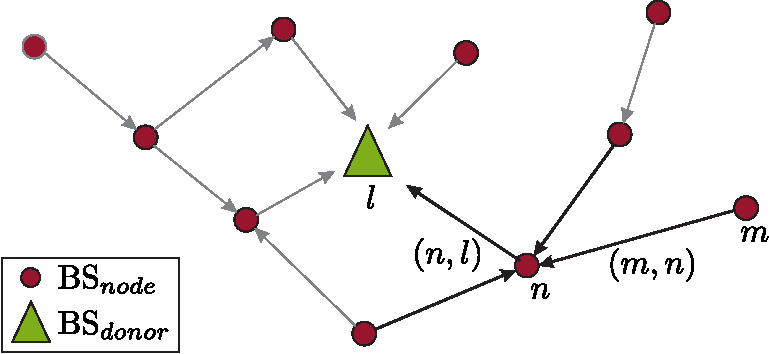
\includegraphics[width=0.6\columnwidth]{Figures/Safehaul/systModelNoWall-eps-converted-to}
      \caption{Example of a graph $\mathcal{G}_i$}
      \label{fig:systModel}
      \vspace{-4mm}
\end{figure}


 Each \node{} $n$ has a finite data buffer with capacity $B^\mathrm{max}_n$ to store the backhaul data to be transmitted to any of the BS-donors. 
 In each time slot $i$, \node{} $n$ is characterized by its load and average queuing time. The load, denoted by $B_{n,i} \in \mathbb{N}$, indicates the number of data packets stored in the buffer at the beginning of time slot $i$. The average queuing time $t^\mathrm{q}_{n,i} \in \mathbb{R}^+$ is the average number of time slots the current packets in the data buffer have been stored.
Additionally, we denote by $M_{n,l,i} \in \mathbb{N}$ the number of data packets transmitted from $n$ and successfully received at $l$ in time slot $i$ (i.e., when $x_{n,l,i}=1$), and with $t^\mathrm{tx}_{n,l,i} \in \mathbb{R^+}$ the transmission time needed to send these packets. Note that $M_{n,l,i}\leq B_{n,i}$ as only packets stored in the data buffer can be transmitted.
At the receiver BS-node $l$, the load $B_{l,i+1}$ of its data buffer is updated at the beginning of the next time slot $i+1$  such that $B_{l,i}+M_{n,l,i}\leq B_l^\mathrm{max}$ holds.
That is to say, packets exceeding the buffer capacity are dropped. Finally, when $x_{n,l,i}=0$ both $M_{n,l,i}$ and $t_{n,l,i}^\mathrm{tx}$ are equal to zero.


We define the maximum tolerable latency $T_\mathrm{max}$ as the maximum time a packet can take from its source \node{} to any BS-donor. Any packet that is not delivered before $T_\mathrm{max}$ milliseconds will be dropped.
 The average maximum end-to-end latency $\bar{T}_{n,d}$ from \node{} $n$ to BS-donor $d$ is the average, over the complete time horizon $I$, of the maximum delay a packet originating from \node{} $n$ takes to reach any BS-donor $d$ in time slot $i$.
This is calculated as $\bar{T}_{n,d} = \frac{1}{I}\sum_{i=1}^I T_{n,d,i}$, 
where $T_{n,d,i}$ is the maximum end-to-end latency among all the packets originating in \node{} $n$ which reach BS-donor $d$ in time slot $i$. 
$T_{n,d,i}$ is a sample of the random variable $T_{n,d}$ drawn from an unknown stationary probability distribution $P$ that depends on the links $x_{n,l,i'}$, $n\in\mathcal{N}$, $l\in{\mathcal{V}}$, $i'=1,\dots,i$, activated up to time $i$, the user's mobility, the location of the \node{} $n$, the interference in the system, and the queue dynamics.
Accordingly, we define the average maximum end-to-end latency in the system $\bar{T}$ as
\begin{equation}
    \bar{T} = \frac{1}{ND}\sum_{n=1}^N\sum_{d=1}^D \bar{T}_{n, N+d}.
    \label{eq:avgDelay}
\end{equation}


 \section{Problem Formulation}
\label{s:prob_formulation}
The joint minimization of the average maximum end-to-end latency and the expected value of its tail loss in IAB-enabled networks is formulated in this section. We first introduce \gls{cvar}, the risk metric accounting for minimizing the events in which the end-to-end latency is higher than $T_\mathrm{max}$. Next, we formulate the optimization problem in the complete network.
 
\subsection{Preliminaries on \gls{cvar}}
Traditionally, latency minimization in IAB-enabled networks has focused on optimizing the expected value of a latency function~\cite{vu2018path, ortiz2019scaros}.
However, such an approach fails to capture the time variability of the latency distribution, thus potentially leading to unreliable systems in which $T_{n,d,i}>T_\mathrm{max}$, for any  $i=1,...,I$, $n\in \mathcal{N}$ and $d\in\mathcal{D}$.
\textit{For this purpose, we consider not only the average end-to-end latency $\bar{T}$ in the system, but also its expected tail loss based on the \gls{cvar}}\cite{Rockafellar2000, Rockafellar2002}.

Having in mind that $T_{n,d}$ is a random variable, we assume it has a bounded mean on a probability space $(\Omega, \mathcal{F}, P)$, with $\Omega$ and  $\mathcal{F}$ being the sample and event space, respectively.
Using a risk level $\alpha\in(0,1]$, the $\mathrm{\gls{cvar}}_\alpha(T_{n,d})$ of $T_{n,d}$ at risk level $\alpha$ quantifies the losses that might be encountered in the $\alpha$-tail. More specifically, it is the expected value of $T_{n,d}$ in its $\alpha$-tail distribution \cite{Rockafellar2002}. 
Formally, $\mathrm{CVaR}_\alpha(T_{n,d})$ is defined as \cite{Rockafellar2000}
\begin{equation}
    \mathrm{CVaR}_\alpha(T_{n,d}) = \min_{q\in\mathbb{R}}\left\{q+\frac{1}{\alpha}\mathbb{E}\left[\max\{T_{n,d}-q,0\}\right]\right\},
    \label{eq:CVaR}
\end{equation}
where the expectation in \eqref{eq:CVaR} is taken over the probability distribution $P$. 
Note that lower $\mathrm{\gls{cvar}}_\alpha(T_{n,d})$ results in higher system reliability because the expected end-to-end latency in the $\alpha$-worst cases is low.
Moreover, note that $\alpha$ is a risk aversion parameter. For $\alpha=1$,  $\mathrm{\gls{cvar}}_\alpha(T_{n,d}) = \mathbb{E}[T_{n,d}]$ which represents the traditional risk-neutral case. 
Conversely, 
$\lim\limits_{\alpha\rightarrow 0}\mathrm{\gls{cvar}}_\alpha(T_{n,d}) = \sup\{T_{n,d}\}$.
\gls{cvar} has been shown to be a coherent risk measure, i.e., it fulfills monotonicity, subadditivity, translation invariance, and positive homogeneity properties \cite{Pflug2000}. 

\subsection{Optimization Problem}
We jointly minimize the average maximum end-to-end latency and its expected tail loss for each \node{}. 
For this purpose, we decide which of the $(n,l)$ links to activate in each time slot $i$ during the finite time horizon $I$.
In the following, we formulate the optimization problem from the network perspective and consider the sum over all \nodes{} in the system. 
The latency minimization problem should consider three different aspects: $(i)$ link activation is constrained by the half-duplex nature of self-backhauling, $(ii)$ only data stored in the data buffers can be transmitted, and $(iii)$ packet drop due to buffer overflow should be avoided.
Formally, the problem is written as:


\small{
\begin{minie}[3]
{\{x_{n,l,i} \}}{\sum_{n\in\mathcal{N}}\left(\sum_{d\in\mathcal{D}}\left(\frac{1}{I}\sum_{i=1}^I T_{n,d,i}\right)+\eta\mathrm{\gls{cvar}}_\alpha(T_{n,f})\right) \label{eq:objective}}{\label{eq:OptProblem}}{}
    \addConstraint{\sum_{\substack{l\in\mathcal{V}, l\neq n}} x_{n,l,i}+\sum_{l\in\mathcal{N}}x_{l,n,i}}{=1,\, \label{eq:constHD}}{n\in\mathcal{N}, \, i=1,\dots,I}
    \addConstraint{ B_{n,i}}{\geq  M_{n,l,i,\, \label{eq:constCausal}}}{ n\in\mathcal{N}, l\in\mathcal{V},\, i=1,\dots,I}
    \addConstraint{ B_{l,j} + M_{n,l,j} \label{eq:constOverflow}}{\leq B^\mathrm{max}_l,\,}{ n\in\mathcal{N}, l\in\mathcal{V},\, i=1,\dots,I}
    \addConstraint{x_{n,l,i}}{\in \{0,1\}, }{n\in \mathcal{N}, l\in \mathcal{V},\, i=1,\dots,I.}
\end{minie}
}

\normalsize
In \eqref{eq:objective}, $\eta \in [0,1]$ is a weighing parameter to control the trade-off between minimizing the average maximum end-to-end latency $\bar{T}_{n,d}$ and the expected loss of its tail.
The constraint in \eqref{eq:constHD} considers half-duplex transmissions by ensuring that, in each time slot $i$, every IAB-node communicates with up to one of its neighbors by either receiving or transmitting backhaul data. \eqref{eq:constCausal} considers data causality, i.e., only data already stored in the data buffers can be transmitted, and \eqref{eq:constOverflow} prevents buffer exhaustion.
As the considered scenario is not static, solving \eqref{eq:OptProblem} would require complete non-causal knowledge of the system dynamics during the complete time horizon $I$. However, in practical scenarios, knowledge about the underlying random processes is not available in advance.
For example, the \node{}'s loads $B_{n,i}$ depend not only on the transmitted and received backhaul data, but also on the randomly arriving data from its users. Similarly, the amounts of transmitted data $M_{n,l,i}$ depend on the varying channel conditions of both BS $n$ and $l$. 
As a result, the exact values of $T_{n,l,i}$, $B_{n,i}$ and $M_{n,l,i}$ are not known beforehand.
For this reason, we present in Sec. \ref{s:algo} \name{}, a multi-agent learning approach to minimize in each \node{} the average maximum end-to-end latency and the expected value of the tail of its loss.
 


 \section{Our proposed solution: \name}
\label{s:algo}
In this section, we describe \name{}, a multi-agent learning approach for the joint minimization of the average maximum end-to-end latency and its expected tail loss in IAB mmWave networks. 
In \name{}, each \node{} independently decides which links $(n,l)$ to activate in every time slot $i$ by leveraging a multi-armed bandit formulation. The consensus among the \nodes{} is reached by exploiting the centralized resource coordination and topology management role of \gls{iab}-donors~\cite[Sec. 4.7.1]{3gpp.38.300}. 

\begin{comment}
For instance, time and frequency resources of the \glspl{du} in the \gls{iab} network can be reserved to particular \node{} by marking them as either \textit{hard} or \textit{unavailable}~\cite[Sec. 10.9]{3gpp.38.300}. Similarly, information regarding the buffer statuses can be retrieved using the related \gls{bap} layer functionality~\cite[Sec. 4.7.3]{3gpp.38.300}.
\end{comment}

\subsection{Multi-Armed Bandit Formulation}
Multi-armed bandit is a tool well suited to problems in which an agent makes sequential decisions in an unknown environment\cite{Sutton2018}. 
In our scenario, each \node{} $n$ decides, in each time slot $i$, which of the links $(n,l)$ to activate without requiring prior knowledge about the system dynamics.
The multi-armed bandit problem at \node{} $n$ can be characterized by a set $\mathcal{A}_n$ of actions and a set $\mathcal{R}_n$ of possible rewards. 
The rewards $r_{n,i} \in \mathcal{R}_n$ are obtained in each time slot $i$ as a response to the selected action $a_{n,i} \in \mathcal{A}_n$
and the observed latency. Since every \node{} $n$ selects only one action during each time slot, we enforce the half-duplex constraint in~\eqref{eq:constHD} by defining the set of possible actions as the set of feasible links for \node{} $n$.
In particular, we define $\mathcal{A}_n$ for $n \in \mathcal{N}$ as $\mathcal{A}_{n} = \{(n,l), (m,n)| m\in \mathcal{N}, \,l\in\mathcal{V} \}$,
where link $(n,n)$ indicates that \node{} $n$ remains idle.
As blockages, overloads, or failures might render certain links $(n,l)$ temporarily unavailable, we define the set $\mathcal{A}_{n,i} \subseteq \mathcal{A}_n$ of available actions  in time slot $i$ as $\mathcal{A}_{n,i} = \{(n,l), (l,n)|(n,l), (l,n) \in \mathcal{E}_i \}$.
Selecting action $a_i=(n,l)$ in time slot $i$ implies $x_{n,l,i}=1$.

The rewards $r_{n,i}$ are a function of the end-to-end latencies ${T}_{n,d,i}$ and depend on whether at \node{} $n$ a link $(n,l)$ or $(l,n)$ is activated. 
\node{} $n$ is connected to the \donor{} via multi-hop wireless links. 
Consequently, $T_{n,d,i}$ cannot be immediately observed when a link $(n,l)$,  with $l \notin \mathcal{D}$ is activated.
In fact, the destination \donor{} $d$ might not even be known to \node{} $n$ in time slot $i$.
To overcome this limitation, we define the rewards $r_{n,i}$ as a function of the next-hop's estimated end-to-end latency $\hat{T}_{l,d,i}$ as
\begin{equation}
r_{n,i}=\begin{cases}
t^\mathrm{q}_{l,i} + t^\mathrm{tx}_{n,l,i} + \hat{T}_{l,d,i}, &\text{for link } (n,l) \\
t^\mathrm{q}_{n,i} + \hat{T}_{n,d,i}, & \text{for link } (l,n),
\end{cases}
\label{eq:rewards}
\end{equation}
where $\hat{T}_{l,d,i}$ is calculated as $\hat{T}_{l,d,i} = \underset{(l,m) \in \mathcal{E}_i}{\min}\;\hat{T}_{l,m,i}$ and $t_{n,l,i}^\mathrm{tx}$ is calculated based on $M_{n,l,i}$ to ensure the causality constraint in (3c) is fulfilled. Note that the constraint in (3d) cannot be enforced, since multi-armed bandit algorithms learn from the activation of both optimal and suboptimal links.



\subsection{Latency and \gls{cvar} Estimation}
As given in \eqref{eq:rewards}, \node{} $n$ learns which links $(n,l)$ to activate by building estimates of the expected latency $\hat{T}_{n,l}$ associated to each of them.
Let $K_{n,l,i}=\sum_{j=1}^i x_{n,l,i}$ be the number of times link $(n,l)$ has been activated up to time slot $i$. The estimated $\hat{T}_{n,l}$ is updated using the sample mean as 
\begin{equation}
    \hat{T}_{n,l,i+1} = \frac{K_{n,l,i}\hat{T}_{n,l,i} + r_{n,i}}{K_{n,l,i}+1},
    \label{eq:delayEstimateSM}
\end{equation}
where the subindex $i$ is introduced to emphasize that the estimate is built over time.


The \gls{cvar} definition given in \eqref{eq:CVaR} requires $T_{n,d}$ which, as discussed before, is not known a priori. 
Hence, we leverage the \gls{cvar} estimator derived in \cite{Luo2017} to calculate the estimated \gls{cvar} of a link $(n,l)$. Let  $\Tilde{r}_n^1,\dots,\Tilde{r}_n^{K_{n,l,i}}$ be all the rewards received up to time $i$.
The estimated $\widehat{\mathrm{\gls{cvar}}}_i(n,l)$ in time slot $i$ is calculated as \cite{Luo2017}
\begin{equation}
    \widehat{\mathrm{\gls{cvar}}}_i(n,l) := \inf_{t \in \mathbb{R}}\left(t + \frac{1}{\alpha \cdot K_{n,l,i}}\sum_{k=1}^{K_{n,l,i}}[\Tilde{r}^k_{n} - t]^+\right). 
    \label{eq:cvarEstimate}
\end{equation}




Using the estimates in \eqref{eq:delayEstimateSM} and \eqref{eq:cvarEstimate}, \node{} $n$ computes the value $Q_n(a_{n,i}=(n,l))$ associated to the selected action $a_n\in \mathcal{A}_n$, and defined as
\begin{equation}
    Q_n(a_{n,i})=\hat{T}_{n.l,i} + \eta \widehat{\mathrm{\gls{cvar}}}_i(n,l).
    \label{eq:Qvalue}
\end{equation}
Note that \eqref{eq:Qvalue} is aligned with the objective function in \eqref{eq:objective}. Actions with an associated low value $Q_n(a_{n,i})$ lead to lower end-to-end latency and a low expected value on its tail. 










\subsection{Consensus}
\label{s:consensus}
All the \nodes{} independently decide which links to activate based on their estimates of the end-to-end latency. 
As a consequence, conflicting actions may be encountered. 
A conflict occurs when two or more \nodes{} $n$ and $m$ aim at activating a link to a common BS $l$, $l \in \mathcal{V}$, i.e., $x_{n,l,i}=x_{m,l,i}=1$.
We reach consensus by first retrieving the buffer and congestion status of the various \gls{iab}-nodes, leveraging the related \gls{bap} layer functionality~\cite[Sec. 4.7.3]{3gpp.38.300}.
With this information at hand, conflicts are resolved by prioritizing the transmission of the \node{} with the larger queuing times $t^\mathrm{q}_{n,i}$ and loads $B_{n,i}$.
Then, we let the \gls{iab}-donor mark as \textit{unavailable} the time resources of the remaining base stations with conflicting scheduling decisions~\cite[Sec. 10.9]{3gpp.38.300}.
Note that as the learning is performed at each \node{}, only the link activation decision and the weighted sum of $t^\mathrm{q}_{n,i}$ and $B_{n,i}$ are transmitted.
Thus, low communication overhead is achieved.

\subsection{Implementation of \name{}}
Here, we describe how the above-mentioned solution can be implemented in a real system. Specifically, we elaborate on the required inputs and the interactions among the different entities as well as the pseudo-code of \name{}, see Alg. \ref{alg:algo}. 

\name{} is executed at each \node{} $n$. For its implementation, the \gls{mno} provides $\alpha$, $\eta$ and $\mathcal{A}_n$ as an input. $\alpha$ is the risk level parameter that influences the level of reliability achieved in the system. Similarly, $\eta$ controls the impact of the minimization of the latency in the $\alpha$-worst cases on the overall performance. Both parameters, $\alpha$ and $\eta$, are set by the \gls{mno} depending on its own reliability requirements.
The set $\mathcal{A}_n$ depends on the considered network topology, which is perfectly known by the \gls{mno}. $\mathcal{A}_n$ includes all links $(n,l)$ and $(l,n)$ to and from the first-hop neighbors of \node{} $n$.
\begin{algorithm}[t]
\footnotesize
\begin{algorithmic}[1]
    \Require $\alpha$, $\eta$, $\mathcal{A}_n$
    \State Initialize $\hat{T}_{n,l}$, $\widehat{\mathrm{\gls{cvar}}}(n,l)$, and $Q_n$ for all $(n,l) \in \mathcal{E}_1$ \label{line:initEst}
    \State Set counters $K_{n,l}=0$ and initial action $a_{n,1}=(n,n)$ \label{line:initCounter}
	\For {every time slot $i=1,...,I$}
	    \State perform action $a_{n,i}$, observe reward $r_{n,i}$ and increase counter $K_{n,l}$ by one \Comment{Eq. \eqref{eq:rewards}} \label{line:reward}
\State update latency estimate $\hat{T}_{n,l}$ \Comment{Eq: \eqref{eq:delayEstimateSM}} \label{line:updateEstDelay}
		\State update \gls{cvar} estimate $\widehat{\mathrm{\gls{cvar}}}(n,l)$ \Comment{Eq: \eqref{eq:cvarEstimate}} \label{line:updateCvar}
		\State update $Q_n(a_{n,i})$ \Comment{Eq: \eqref{eq:Qvalue}} \label{line:updateQ}
		\State select next action $a_{n,i+1}$ using $\epsilon$-greedy \Comment{Eq. \eqref{eq:epsGreedy}} \label{line:epsGreedy}
		\State share $a_{n,i+1}$, $t^\mathrm{q}_{n,i}$ and $B_{n,i}$ with the other \nodes{} \label{line:share}
		\State if required, update $a_{n,i+1}$ to reach consensus \Comment{Sec. \ref{s:consensus}} \label{line:consensus}
\EndFor
\end{algorithmic}
\caption{\name{} algorithm at each \node{}} \label{alg:algo} 
\end{algorithm}

The execution of \name{} begins with the initialization of the latency and \gls{cvar} estimates, and the values $Q$ of the actions in $\mathcal{A}_n$.
Additionally, the counters $K_{n,l}$, that support the calculations of $\hat{T}_{n,l}$ and $\widehat{\mathrm{\gls{cvar}}}(n,l)$, are initialized for all links in $\mathcal{A}_n$ (lines \ref{line:initEst}-\ref{line:initCounter}).
These parameters are updated and learnt throughout the execution of \name{}.
At time slot $t=0$, no transmission has occurred and $B_{n,0}=0$. Hence, \node{} $n$ remains idle for the first time slot $i=1$, i.e., $a_{n,1}=(n,n)$ (line \ref{line:initCounter}).
Next, and in each of the subsequent time slots $i\in \{1,\ldots, I\} $, the selected action is performed and the corresponding reward is obtained (line \ref{line:reward}).
If \node{} $n$ transmits in time slot $i$, i.e., $a_{n,i}=(n,l)$, the reward $r_{n,i}$ is sent by the receiving BS $l$ through the control channel.
If $a_{n,i}=(l,n)$, the reward $r_{n,i}$ depends, as given in \eqref{eq:rewards}, only on the current estimates at \node{} $n$ and the status of its buffer $B_{n,i}$.
With the observed reward $r_{n,i}$, the counter for action $a_{n,i}$ is increased and the latency and \gls{cvar} estimates are updated (lines \ref{line:reward}-\ref{line:updateCvar}).
Using the new estimates (lines \ref{line:updateEstDelay} and $\ref{line:updateCvar}$), the value $Q(a_{n,i})$ of the performed action $a_{n,i}$ is updated (line \ref{line:updateQ}).
The next action $a_{n,i+1}$ is then selected according to $\epsilon$-greedy (line \ref{line:epsGreedy}), which is a well-known method to balance the exploitation of links with estimated low latency, and the exploration of unknown but potentially better ones.
In $\epsilon$-greedy, a random action $a_{n,i+1}$ from the set $\mathcal{A}_{n,i+1}$ is selected with probability $\epsilon \in [0,1]$.
With probability $(1-\epsilon)$, instead, the action that yields the estimated lowest value is chosen, i.e., 
\begin{equation}
a_{n,i+1} = \begin{cases}
\text{randomly selected action from } \mathcal{A}_{n,i+1}, & \text{if } x\leq\epsilon \\
\underset{b_n \in \mathcal{A}_{n,i+1}}{\argmax} \, Q_n(b_{n}), & \text{if } x>\epsilon, 
\end{cases}
    \label{eq:epsGreedy}
\end{equation}
where $x$ is a sample taken from a uniform distribution in the interval $[0,1]$.
Once the action $a_{n,i+1}$ is selected, it is shared with other \nodes{} in the network along with $t^\mathrm{q}_{n,i}$ and $B_{n,i}$ (line \ref{line:share}).
As described in Section~\ref{s:consensus}, this goes through the control channel. 
If conflicts arise, consensus is reached by prioritizing the transmission of the \node{} with the largest loads and queuing times (line \ref{line:consensus}).

\subsection{Regret Analysis}
The regret $\zeta$ is defined as the expected loss caused by the fact that the optimal action is not always selected \cite{Auer2002}. 
Let $\bar{T}^*$ and $\Bar{T}_{a_n}$ be the expected delay associated to the optimal action $a^* \in \mathcal{A}_n$ and the non-optimal action $a_n \in \mathcal{A}_n$, respectively. Similarly, let $\mathrm{\gls{cvar}}^*$ and $\mathrm{\gls{cvar}}_{a_n}$ be the \gls{cvar} of the optimal action $a^* \in \mathcal{A}_n$ and the non-optimal action $a_n\in \mathcal{A}_n$, respectively.
Formally, the regret $\zeta_i$ after $i$ time slots is defined as
\begin{align}
\label{eq:regret}
    \zeta_i &=\!\! \sum_{a_n \in \mathcal{A}_n}\!\left( \left(\Bar{T}_{a_n} + \eta\mathrm{\gls{cvar}}_{a_n}\right) - \left(\Bar{T}^* + \eta\mathrm{\gls{cvar}}^*\right)\right)\mathbb{E}[K_{a_n,i}]  \nonumber \\
    &= \!\! \sum_{a_n \in \mathcal{A}_n}\Delta_{a_n}\mathbb{E}[K_{a_n,i}], 
\end{align}
where $K_{a_n,i}$ is the number of times action $a_n$ has been selected up to time slot $i$.

\begin{proposition}
\label{prop:probNonOptArm}
For a network $\mathcal{G}$ in which the independent decisions of the \nodes{} do not lead to conflicts, let
$A_n=|\mathcal{A}_n|$ be the number of available actions for \node{} $n$. Additionally, let $c > 0$, $0 < d \leq 1$, and $\epsilon_i := \min(1, \frac{cA_n}{d^2i})$.
Then, there exists a positive constant $C > 1$, such that the probability that \name{} chooses a non-optimal action $a_n \neq a^*$ after $i\geq cA_n/{d}$ time slots is upper bounded as
\begin{align*}
\mathbb{P}[a_{n,i} = a_n] \leq & \frac{c}{d^2i} + \frac{4e}{d^2}B_i^{\frac{c}{2}} + \frac{2Cd^2}{c \mathrm{ln}\left(\frac{(i-1)d^2e^{0.5}}{cA_n}\right)} \\
    & + 4C\left(\frac{c}{d^2}\mathrm{ln}\left(\frac{(i-1)d^2e^{0.5}}{c A_n}\right)\right) B_i^{\frac{c}{5d^2}},
\end{align*}
with $B_i = \frac{c A_n}{(i-1)d^2e^{0.5}}.$
\end{proposition}
\begin{proof}
See the Appendix.
\end{proof}

\begin{theorem}
\label{theo:regret}
For a network $\mathcal{G}$ in which the independent decisions of the \nodes{} do not lead to conflicts, the regret $\zeta_i$ of \name{} after $i$ time slots is upper bounded by
\begin{align*}
    \zeta_i \leq \!\!\sum_{a_n\in \mathcal{A}_n} & \!\!\Delta_{a_n} \!\!\left(1+\sum_{i'=2}^i\left[ \frac{c}{d^2i'} + \frac{4e}{d^2}B_{i'}^{\frac{c}{2}} +  \frac{2Cd^2}{c \mathrm{ln}\left(\frac{(i'-1)d^2e^{0.5}}{cA_n}\right)}\right.\right. \\ 
    & + \left.\left. 4C\left(\frac{c}{d^2}\mathrm{ln}\left(\frac{(i'-1)d^2e^{0.5}}{c A_n}\right)\right) B_{i'}^{\frac{c}{5d^2}} \right]\right),
\end{align*}
where 
$c > 0$ and $0 < d \leq 1$.
\end{theorem}

\begin{proof}
From the definition in \eqref{eq:regret}, the regret can be upper bounded as 
\begin{equation}
\zeta_i \leq \sum_{a_n\in\mathcal{A}_n}{\Delta_{a_n} \left(1+\sum_{i'=2}^i\mathbb{P}[a_{n,i'}=a_n]\right)} \label{eq:regret2},
\end{equation}
by considering that $\mathbb{E}[K_{a_n,i}]\leq 1+\sum_{i'=2}^i\mathbb{P}[a_{n,i'}=a_n]$. 
The bound is obtained by including the result of Proposition \ref{prop:probNonOptArm} in \eqref{eq:regret2} as
\begin{align}
    \zeta_i \leq \!\!\sum_{a_n\in \mathcal{A}_n} & \!\! \Delta_{a_n}\!\! \left(1+\sum_{i'=2}^i\left[ \frac{c}{d^2i'} + \frac{4e}{d^2}B_{i'}^{\frac{c}{2}}  + \frac{2Cd^2}{c \mathrm{ln}\left(\frac{(i'-1)d^2e^{0.5}}{cA_n}\right)}
    \right.\right. \nonumber \\
    &+ \left.\left. 4C\left(\frac{c}{d^2}\mathrm{ln}\left(\frac{(i'-1)d^2e^{0.5}}{c A_n}\right)\right) B_{i'}^{\frac{c}{5d^2}}  \right]\right),
\end{align}
As every term in square brackets decreases monotonically in $i'$, the regret $\zeta_i$ grows sub-linearly.

\end{proof}  \section{Simulation setup}
\label{s:simulation_setup}
Given the lack of access to actual 5G (and beyond) network deployments, prior works mostly rely on \textit{home-grown} simulators for performance evaluation. Although this is a valid approach, these simulators often cannot fully capture the real network dynamics, introducing strong assumptions in the physical and/or the upper layers of the protocol stack. 
Until very recently, the most complete  simulator for \gls{iab} networks was a system-level simulator~\cite{8514996} developed as an extension of the ns-3 \textit{mmWave} module~\cite{8344116}. However, despite accurate modeling of the \gls{iab} protocol stack, it is currently behind the latest \gls{iab} specifications\footnote{For instance due to the assumption of L-3 (instead of L-2) relaying at the \gls{iab}-nodes which was based on a draft version of TR 38.874~\cite{3gpp_38_874_old}.}. Moreover, the ns-3 \gls{iab} extension is unsuitable for large simulations with hundreds of nodes due to reliance on an older version of the \textit{mmWave} module. Therefore, in our work we opt for Sionna~\cite{hoydis2022sionna}, which is an open-source GPU-accelerated toolkit based on TensorFlow. 

However, unlike the aforementioned ns-3 module, Sionna is a physical layer-focused simulator that does not explicitly model 5G networks, thus lacking  the characterization of the 5G-NR upper-layer protocol stack. Hence, we extend Sionna by including the system-level functionalities such as MAC-level scheduling and RLC-level buffering. Furthermore, since Sionna exhibits slight differences compared to the 5G-NR physical layer, we extend Sionna's physical layer model~\cite{hoydis2022sionna} with the 5G-NR procedures. In the following, we describe the details of our extensions, which are publicly available\footnote{\url{https://github.com/TUDA-wise/safehaul_infocom2023}}.


\begin{figure}[t!]
    \centering
    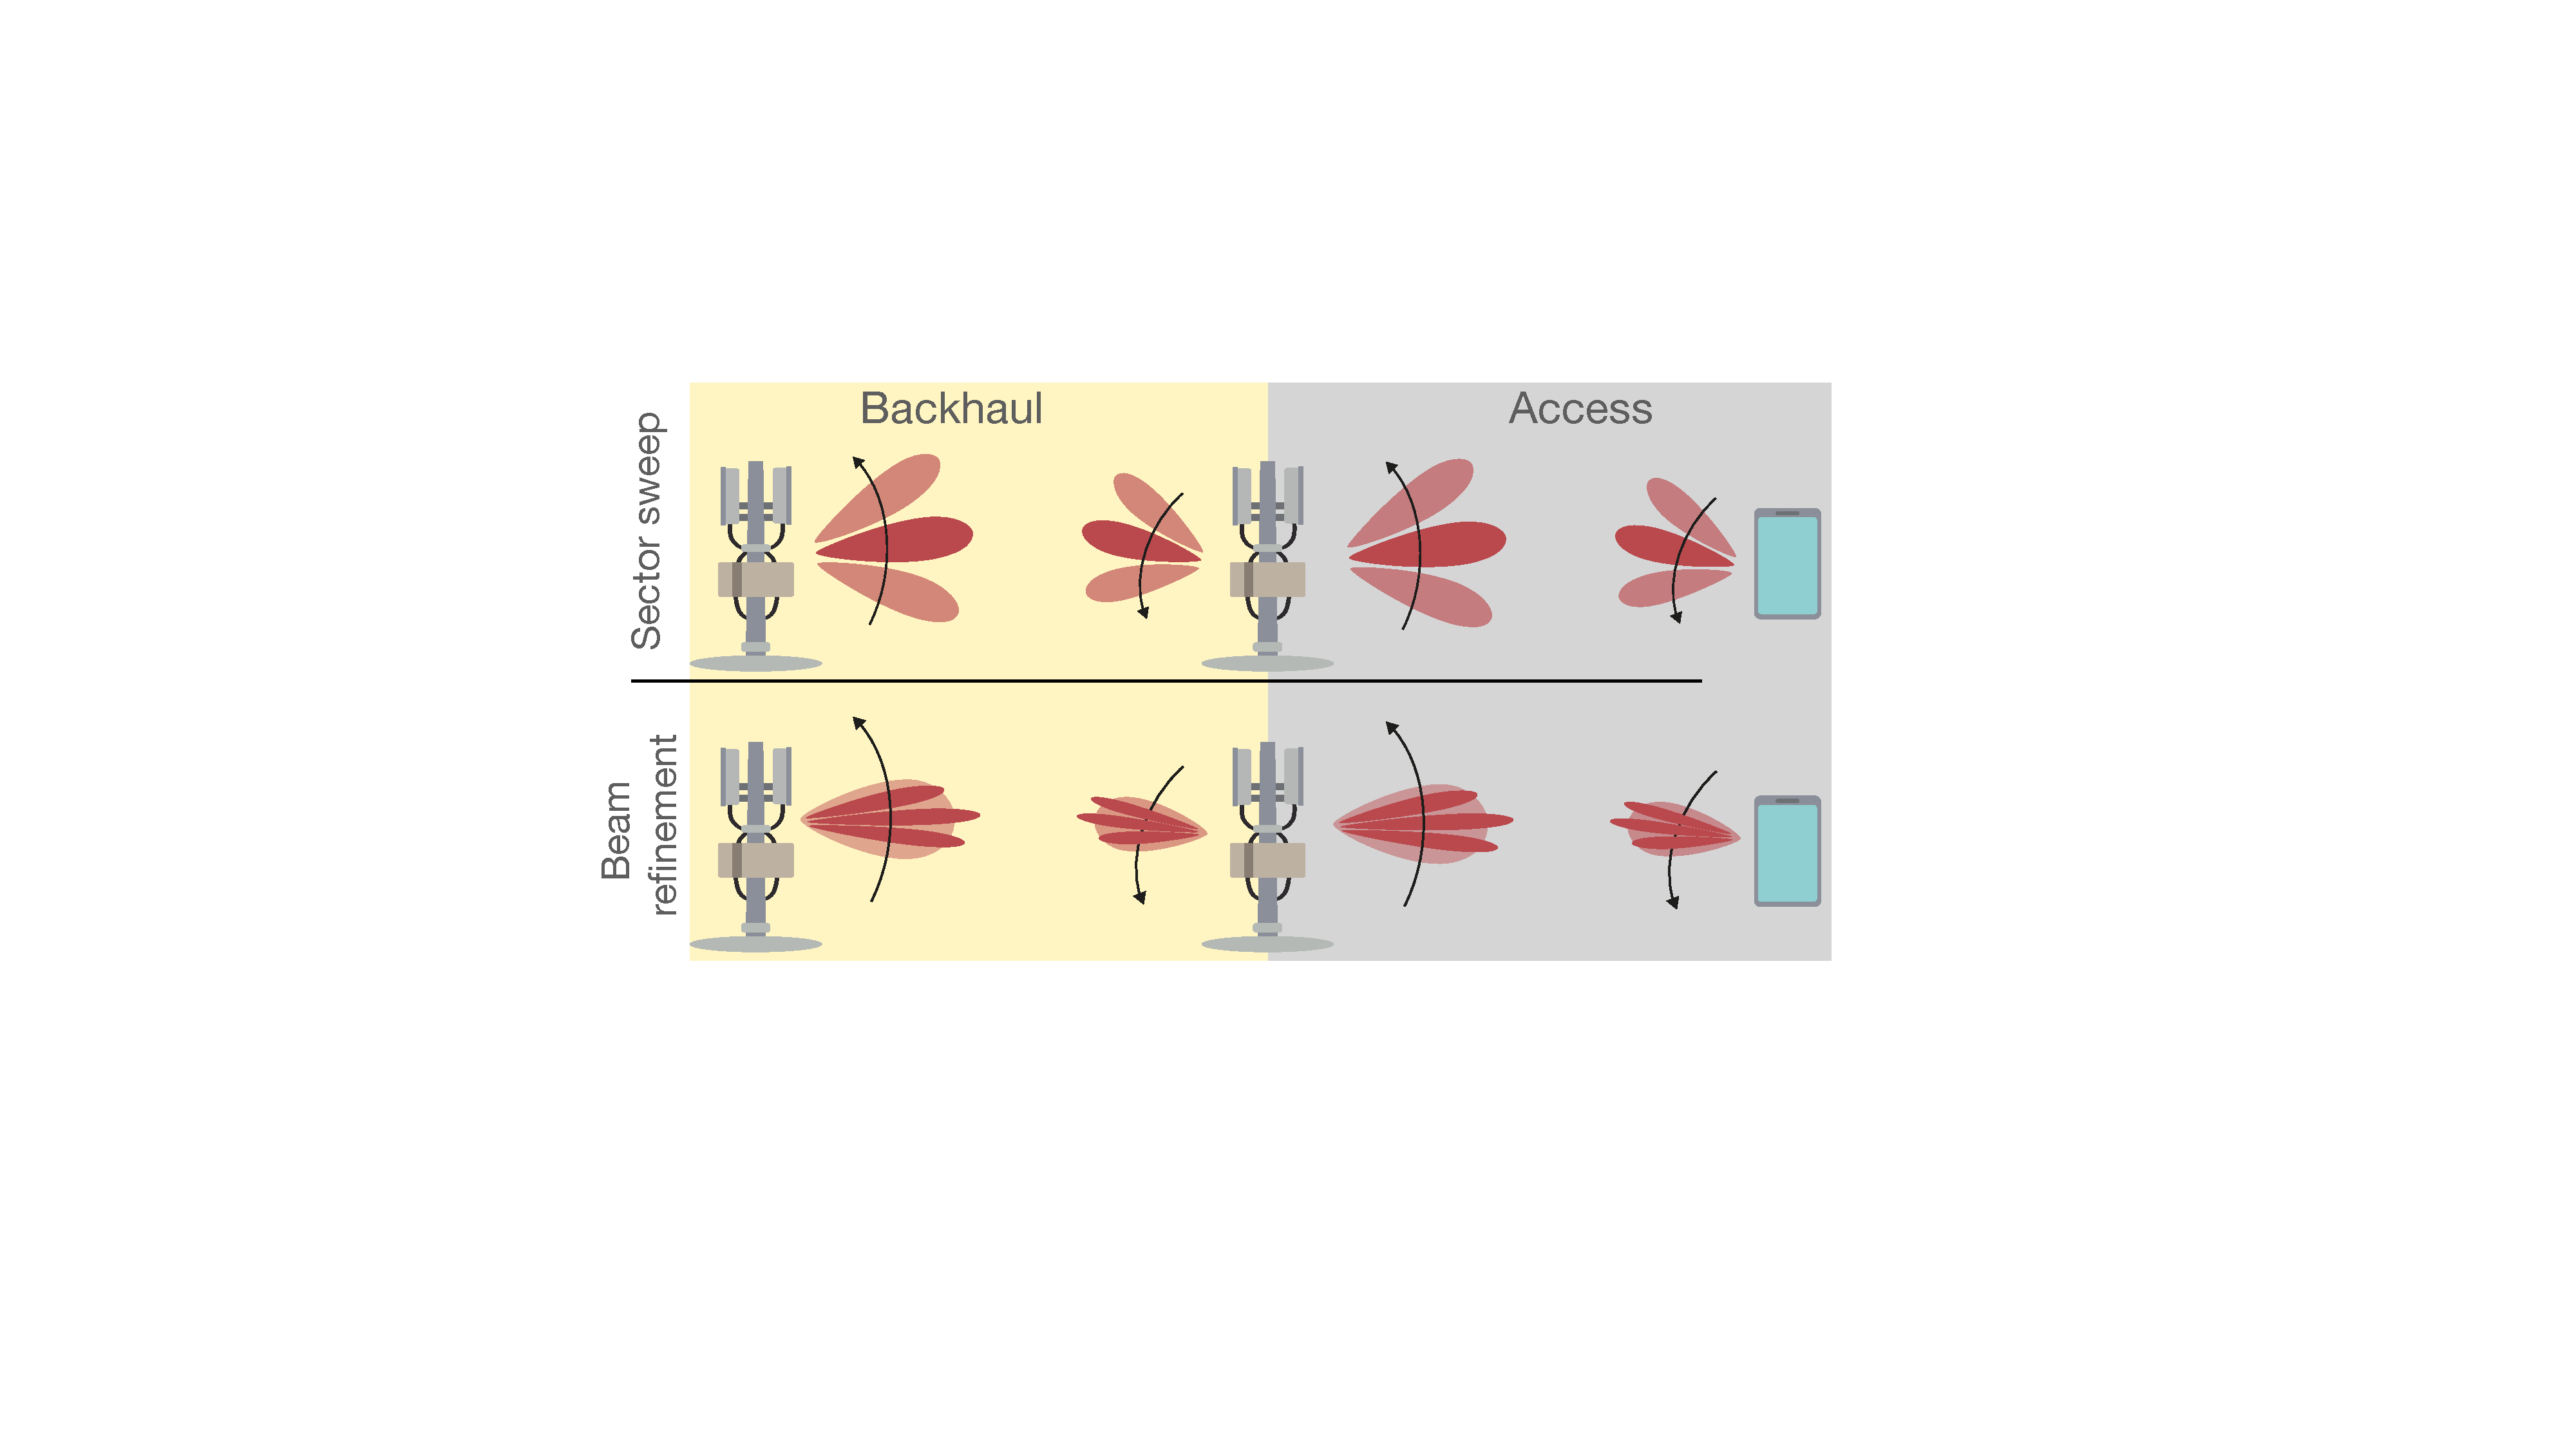
\includegraphics[scale=0.18]{Figures/Safehaul/Beamforming-2.pdf}
      \caption{Schematic of the hierarchical beam management procedure. First, the general direction is estimated using wide beams (top). Then, the search is refined using the narrow beams codebook.}
      \label{fig:beamforming}
      \vspace{-5mm}
\end{figure}



\subsection{Extensions to Sionna's physical layer module}
\label{sub:additionalSionna}
In this section, we describe the physical layer modification that were necessary to evaluate IAB scenarios using Sionna. 

\subsubsection{Codebook-based Beamforming}
Sionna's native beamforming only supports \gls{zf} pre-coding in downlink. Therefore, as a first step, we extend Sionna by implementing an NR-like codebook-based analog beamforming both at the transmitter and at the receiver.
Specifically, we assume that the beamforming vectors at the transmitter $w_{tx}$ and at the receiver $w_{rx}$ are a pair of codewords selected from a predefined codebook. The codebook is computed by defining a set of beam directions $\{ \omega_{p,q} \}$ which scans a given angular sector with a fixed beamwidth. The steering vector $a_{p,q}$ corresponding to direction $\omega_{p, q}$ can be computed as:
\medmuskip=1mu
\thinmuskip=1mu
\thickmuskip=1mu
\begin{equation}
    \begin{aligned}
            a_{p,q} &= \left[ 1,\ldots, e^{j\frac{2\pi}{\lambda}d\left(i_{ H}\sin\alpha_p\sin\beta_q+i_{V}\cos\beta_q\right)}, \ldots,  \right. \\ 
            & \left. e^{j\frac{2\pi}{\lambda}d\left((N_{H}-1)\sin\alpha_p\sin\beta_q + (N_{ V}-1)\cos\beta_q\right)} \right] ^T,
    \end{aligned}
\end{equation}
\medmuskip=6mu
\thinmuskip=6mu
\thickmuskip=6mu
where $N_{H}$ and $N_{V}$ are the number of horizontal and vertical antenna elements, respectively. The horizontal and vertical indices of a radiating element are denoted by $i_{H}\in \{0, \ldots, N_{H} - 1 \}$ and $i_{V}\in \{0, \ldots, N_{V} - 1\}$, respectively. $\alpha_p$ and $\beta_q$ represent the azimuth and elevation angles of $\omega_{p, q}$. Next, we define the codebook as the set $\{ \left( \sqrt{N_{H} N_{V}} \right)^{-1} w_{p, q} \}$. 

In line with the 5G-NR beam management procedure~\cite{giordani2018tutorial}, we assume the lack of complete channel knowledge, i.e., the communication endpoints do not know the corresponding channel matrix. Accordingly, an exhaustive search is conducted to identify the best pair of codewords resulting in the highest \gls{sinr}. We leverage a hierarchical search, in which the communication pairs first perform a wide-beam search
in which the transmitter and the receiver approximate the direction of communication, see Fig.~\ref{fig:beamforming}. Next, the beamforming direction is fine-tuned through a beam refinement procedure going through a codebook with narrow beams. Consequently, we employ two types of codebooks, one with wide beams for sector sweep and another with narrow beams for beam refinement.   

\subsubsection{SINR Computations}

Since Sionna does not natively calculate the \gls{sinr}, we add this functionality to the simulator to better model the impact of interference in our simulations. We compute the \gls{sinr} experienced by \glspl{tb} by combining the power of the intended signal with that of the interferers and of the thermal noise. Specifically, we first compute the power $P_{n}(i,f)$ of the intended signal at receiver $n$ over frequency $f$ and in time slot $i$. Then, we obtain the overall interference power by leveraging the superposition principle and summing the received power from all other interfering base stations $P_{m} (i, f)$ where $m \neq n$. For the purposes of this computation, we assume that each interferer employs the beamforming vector yielding the highest \gls{snr} towards its intended destination. Similarly, the transmitter and the receiver use the beamforming configuration estimated via the hierarchical search procedure. Finally, the \gls{sinr} is $
\label{EQ_CGAN1}
\gamma_{n} (i, f)= \frac{P_{n}(i,f)}{\sum\limits_{m \neq n} P_{m}(i,f) + \sigma^2(i,f)}
$
where $\sigma^2(i,f)$ is the thermal noise power at the receiver.

\begin{figure}
\centering
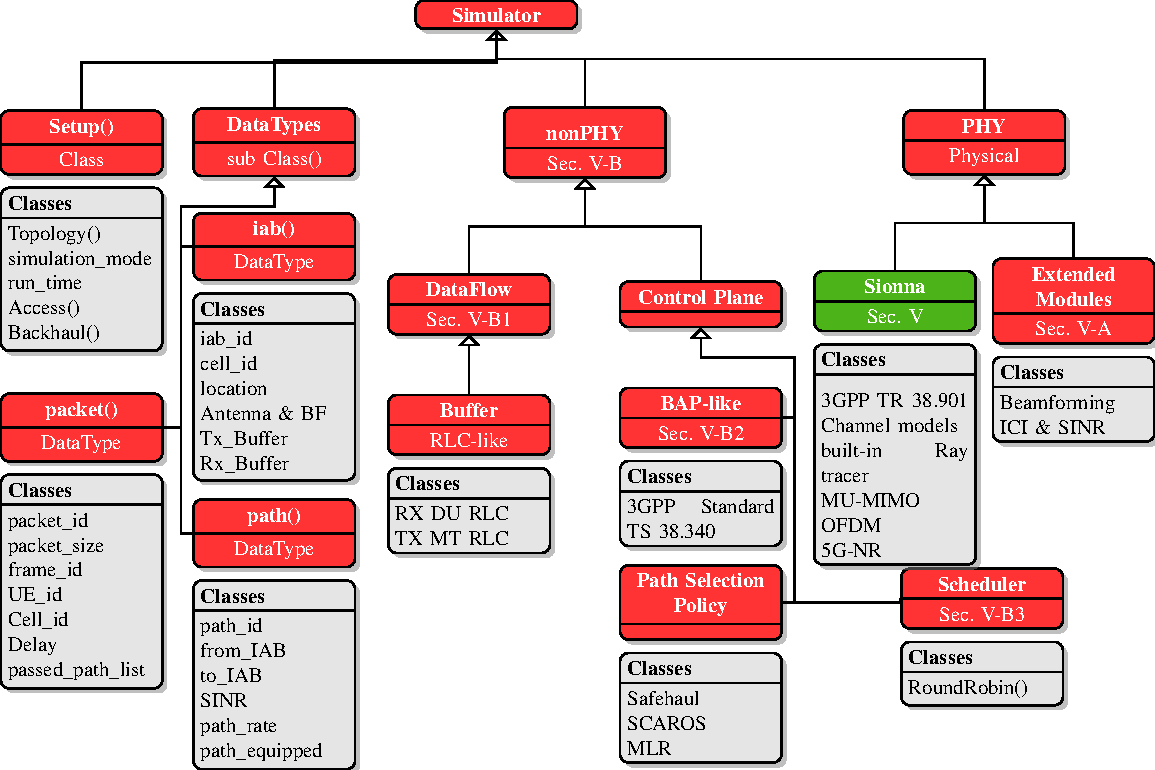
\includegraphics[width=0.7\textwidth]{Figures/Safehaul/simulator_diagram.pdf}
\label{bigpicture}
\caption{Overall design of our Sionna's extension. The red blocks represent our additions to the baseline simulator, i.e., Sionna~\cite{hoydis2022sionna}.}
\end{figure}

As mentioned, Sionna is mainly a physical layer simulator. However, to get closer to \gls{iab} networks as specified in Rel. 17, we have extended Sionna by implementing a selection of system-level features. To such end, we introduced a discrete-event network simulator for modeling \gls{iab} networks. This system-level extension operates on top of Sionna and provides basic functionalities such as a \gls{mac}-level scheduler, layer-2 buffers, and data flow and path selection mechanisms. Our simulator, depicted in Fig.~\ref{fig:simulator_design}, generates a variety of system-level KPIs such as latency, throughput, and packet drop rate. 


\subsubsection{Data Flow and buffer}
\label{sub:Dataflow}
3GPP has opted for a layer-2 relaying architecture for \nodes{} where hop-by-hop \gls{rlc} channels are established. This enables retransmissions to take place on the affected hops only, thus preventing the need for traversing again the whole route from the \donor{} whenever a physical layer \gls{tb} cannot be successfully decoded. This design results in a more efficient recovery from transmission failures and reduces buffering at the communication endpoints~\cite{madapatha2020integrated}. To mimic this architecture, we have implemented RLC-like buffers at each base station. Specifically, each \node{} features layer-2 buffers for both received and transmitted packets.
For instance, the data flow for an uplink packet is the following.
The \gls{ue} generates packets and sends a transmission request to the base station. Consequently, the scheduler allocates OFDM symbols for this transmission, which is eventually received and stored at the RX buffer of its \gls{du}. Next, the packet is placed into the TX buffer to be forwarded to the suitable next hop \node{}. This procedure is repeated until the packet crosses all the wireless-backhaul hops and reaches the \donor. Note that the packet can be dropped due to latency constraints or to interference.

\subsubsection{\gls{bap}}
\label{sub:bap}
To manage routing within the wireless-backhauled network, the 3GPP introduced \gls{bap}, i.e., an adaptation layer above \gls{rlc} which is responsible for packet forwarding between the \donor{} and the access \nodes~\cite{3gpp_38_340}. Our simulator mimics this by associating each \node{} to a unique \gls{bap} ID. Moreover, we append a \gls{bap} routing ID to each packet at its entry point in the \gls{ran} (i.e., the \donor{} and the \glspl{ue} for DL and UL data, respectively).  Then, this identifier is used to discern the (possibly multiple) routes toward the packet's intended destination~\cite{3gpp_38_340}. The choice of the specific route is managed by \name{}.


\subsubsection{Scheduler}
\label{sub:scheduler}
Finally, we implemented a \gls{mac}-level scheduler which operates in a \gls{tdma} mode. The scheduler periodically allocates the time resources to backhaul or access transmissions in a Round-Robin fashion\footnote{The choice of the specific scheduling algorithm is outside of the scope of the 3GPP NR specifications, and is thus left to the MNOs. Accordingly, a Round-Robin scheduling policy represents a typical baseline assumption.}. Specifically, each cell first estimates the number of OFDM symbols needed by each data flow by examining the corresponding buffer. Then, the subframe's OFDM symbols are equally allocated to the users. If a user requires fewer symbols to transmit its complete buffer, the excess symbols (the difference between the available slot length and the needed slot length) are distributed to the other active users. \section {Performance Evaluation}
\label{s:simulation_analysis}

\begin{figure}
    \centering
    \subfloat[][Manhattan (223 \nodes{}).]{
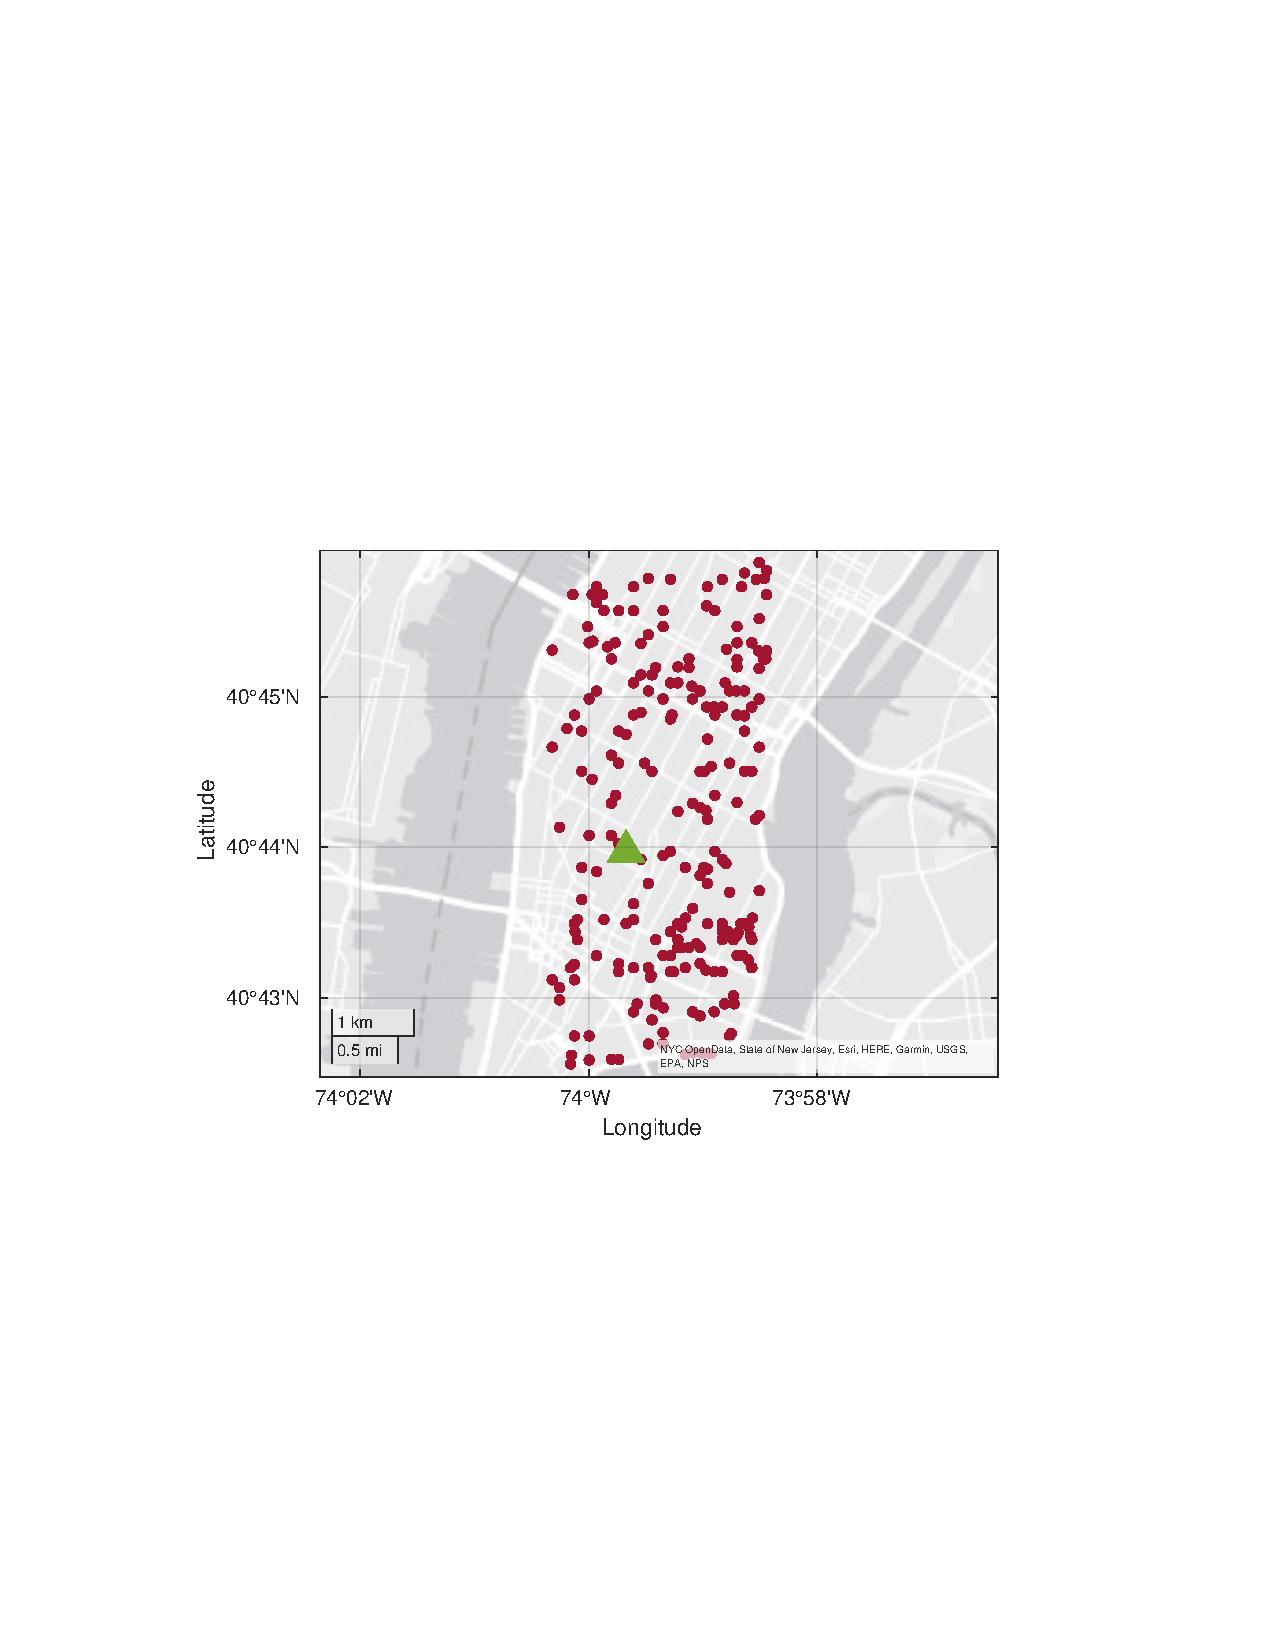
\includegraphics[scale=0.3]{Figures/Safehaul/manhattan_new.pdf}
    \label{fig:manhattan}}
    \subfloat[][Padova (100 \nodes{}).]{
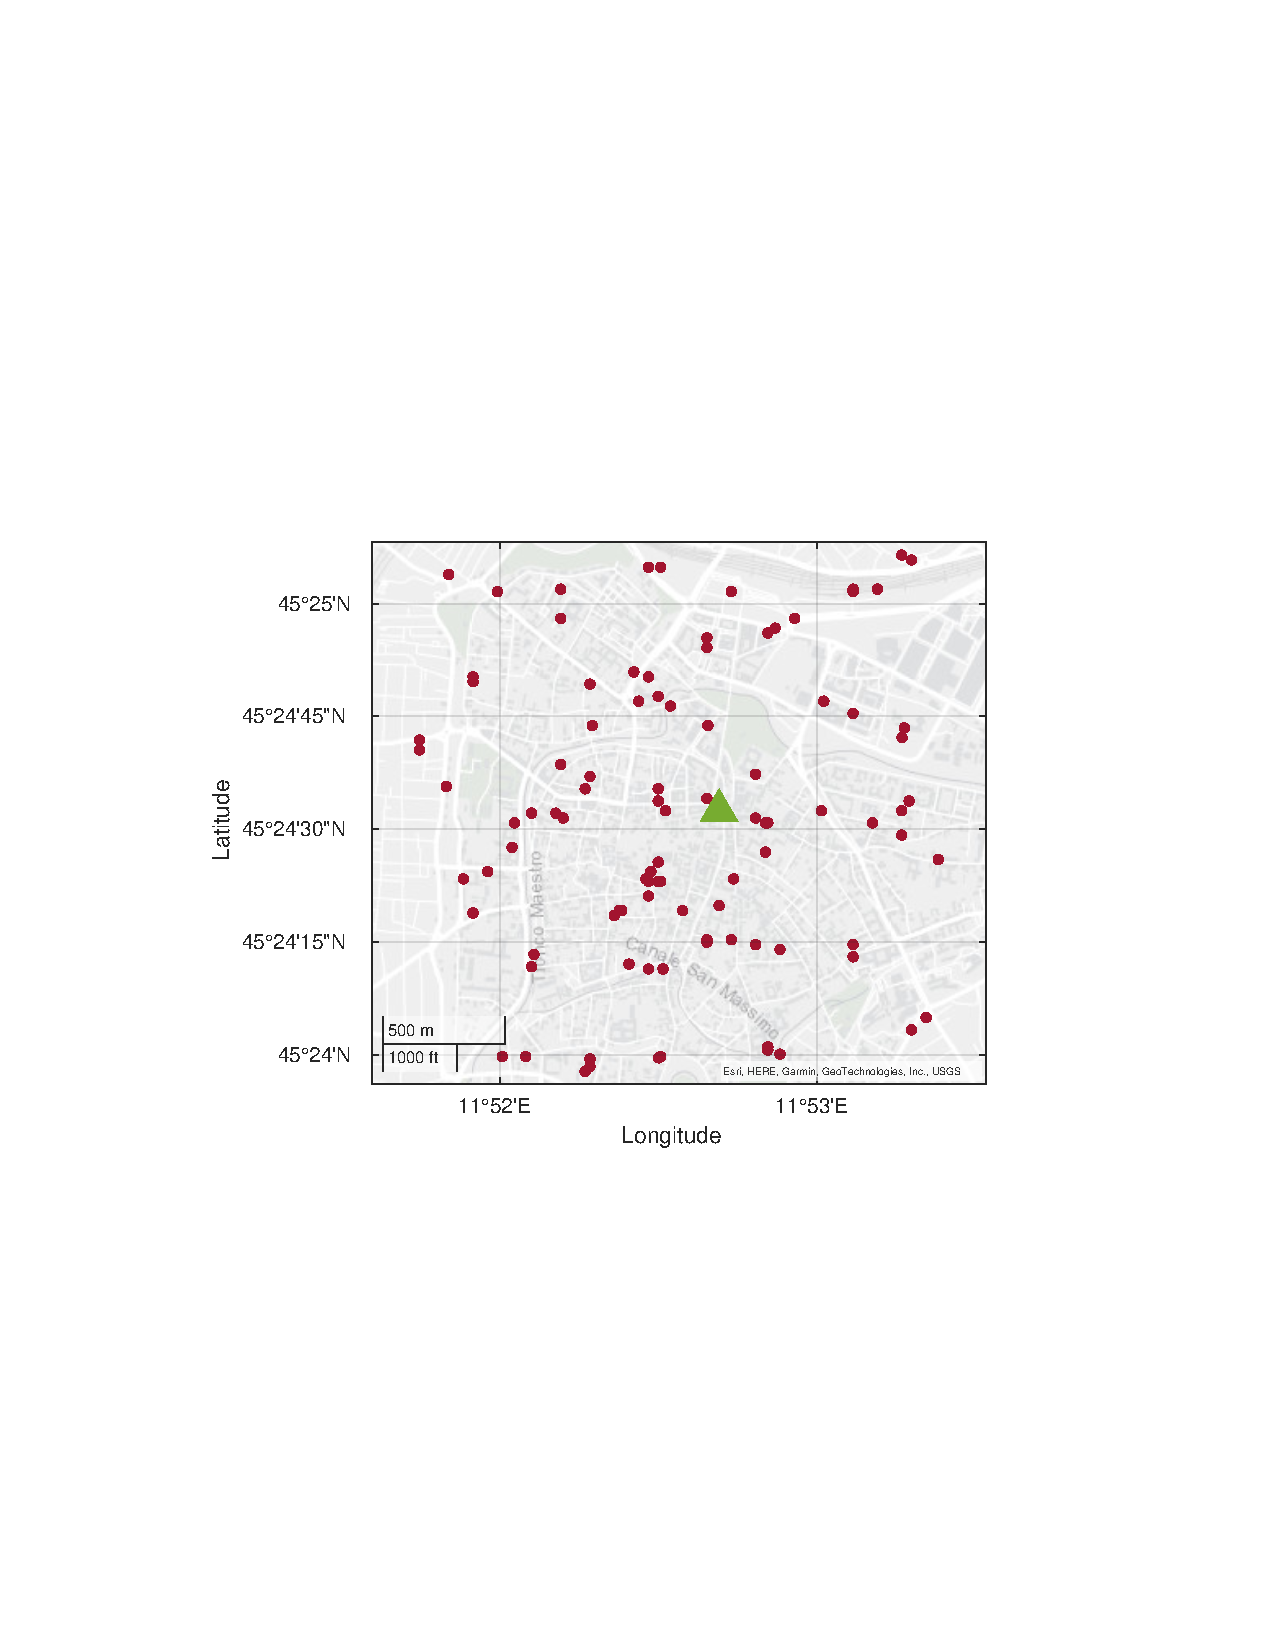
\includegraphics[scale=0.3]{Figures/Safehaul/padova_new.pdf}
    \label{fig:Padova_Map}}
    \caption{Locations of \nodes{} (red dots) and of the \donor{} (green triangle) in the Manhattan (left) and Padova (right) topologies.}
\end{figure}


\begin{figure*}[t!]
\centering
\subfloat[][Average per-UE end-to-end latency]{
    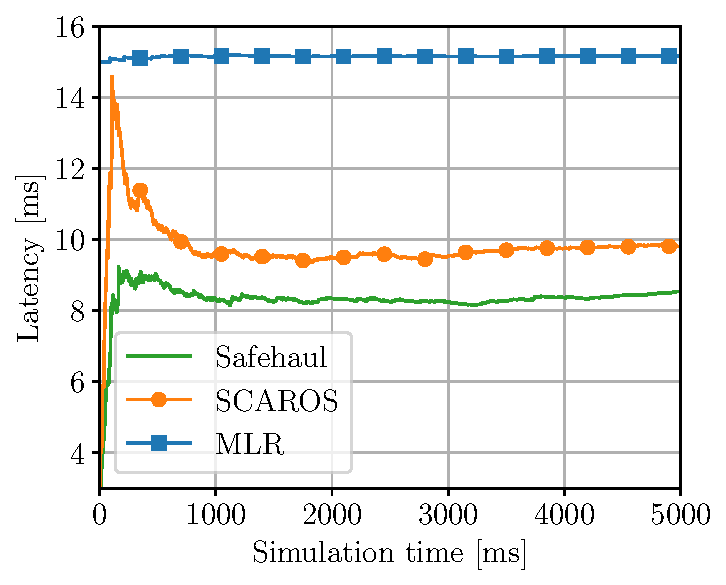
\includegraphics[width=.25\linewidth]{Figures/Safehaul/S1_lat_vs_time.pdf}
    \label{fig:avgE2EDelay}
    }
\subfloat[][Average per-UE throughput]{
    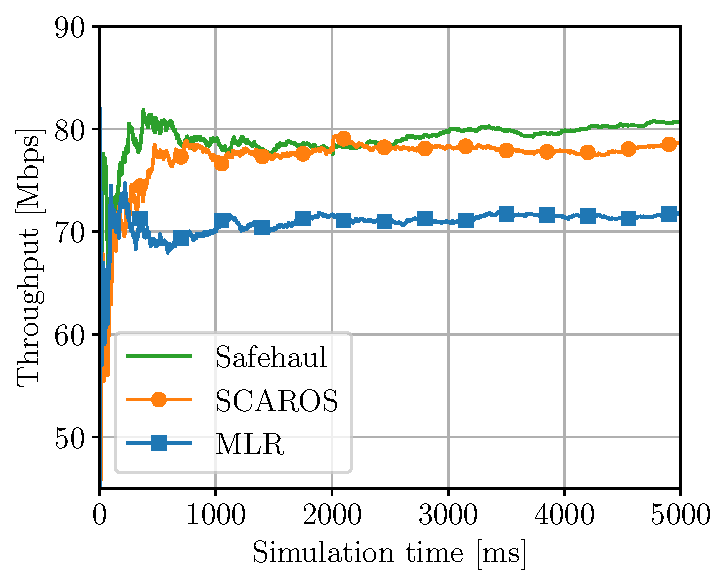
\includegraphics[width=.25\linewidth]{Figures/Safehaul/S1_thr_vs_time.pdf}
    \label{fig:avgTput}
    }
\subfloat[][Average per-UE packet drop rate]{
    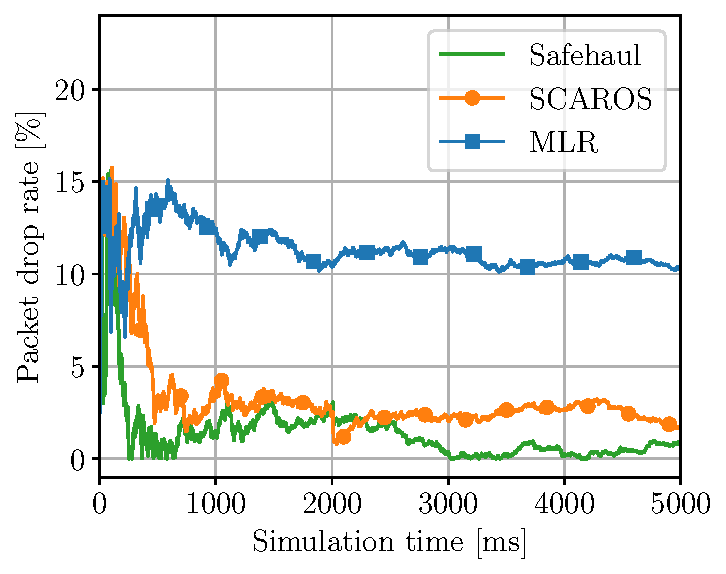
\includegraphics[width=.25\linewidth]{Figures/Safehaul/S1_drop_vs_time.pdf}
    \label{fig:avgDropRate}
    }
  
\caption{Average network performance for $50$ \glspl{ue} and $80$~Mbps per-UE source rate (Scenario 1).}
  \label{fig:avgNetPerfomance}
\end{figure*}
\begin{figure*}
\centering
\subfloat[][Per-UE end-to-end Latency]{
    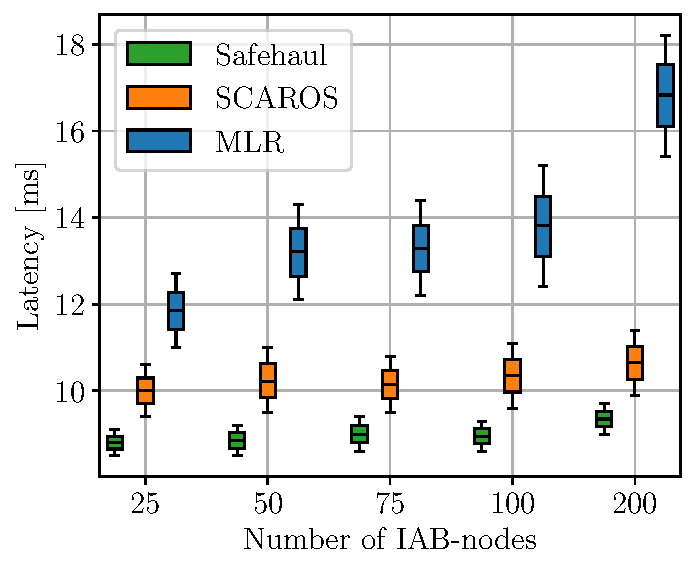
\includegraphics[width=.25\linewidth]{Figures/Safehaul/S2_lat.pdf}
    \label{fig:avgE2EDelay_s2}
    }
\subfloat[][Per-UE throughput]{
    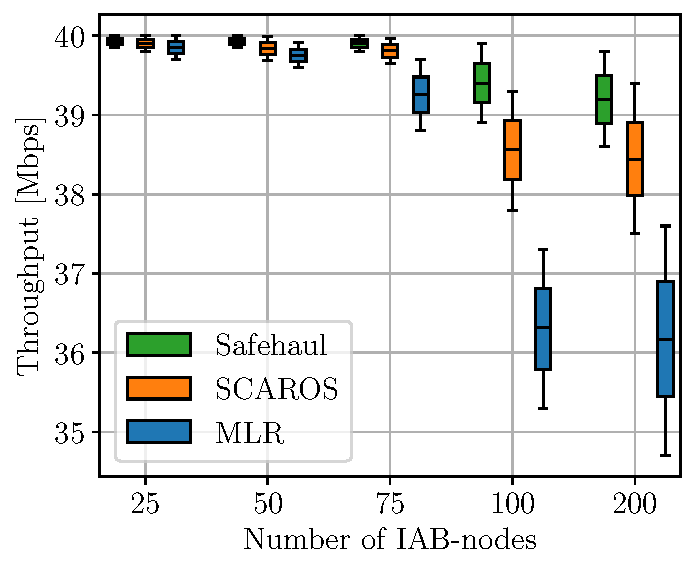
\includegraphics[width=.25\linewidth]{Figures/Safehaul/S2_thr.pdf}
    \label{fig:avgTput_s2}
    }
\subfloat[][Per-UE packet drop rate]{
    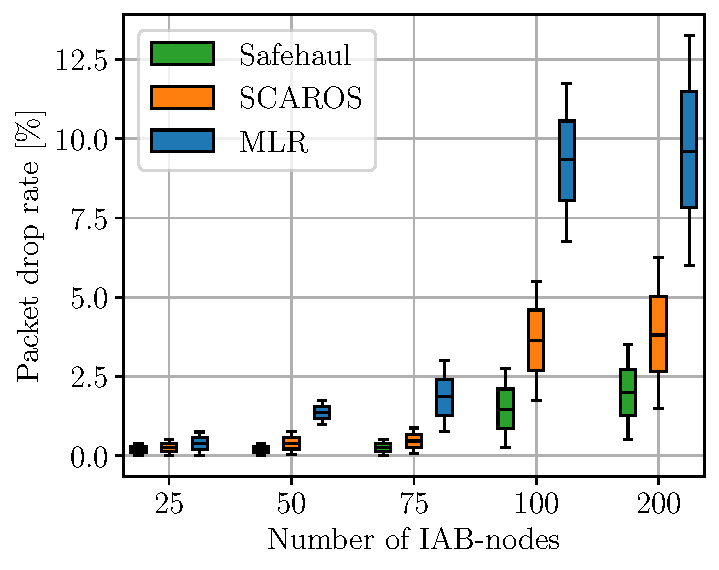
\includegraphics[width=.25\linewidth]{Figures/Safehaul/S2_drop.pdf}
    \label{fig:avgDropRate_s2}
    }
  
   \caption{Network performance for $\{25, 50, 75, 100, 200\}$ \node{}, $2$ UEs per \nodes{} on average, and $40$ Mbps per-UE source rate (Scenario 2).}
  \label{fig:avgNetPerfomance_s2}
  \vspace*{-3mm}
\end{figure*}

In our simulations, we consider realistic cellular base station deployments in Manhattan, New York City\footnote{The locations correspond to the network of T-Mobile, which has the largest deployment among the \glspl{mno}.} and in the historical city center of Padova. Specifically, for the former we collect the locations of $N=223$ 5G-NR base stations in an area of 15~$\text{Km}^2$ as depicted in Fig.~\ref{fig:manhattan}. On the other hand, in the Padova topology we combine locations of $N=100$ 4G-LTE \gls{bs} of different \glspl{mno} (WINDTRE, TIM, and Vodafone) in an area of 10~$\text{Km}^2$ as depicted in Fig.~\ref{fig:Padova_Map}, due to the lack of 5G-NR base station deployment at the time of writing of this paper. The detailed simulation parameters are provided in Table \ref{Tab:parameters}. We used the channel model outlined by 3GPP in TR 38.901 \cite{3gpp.38.901}, which provides a statistical channel model for 0.5-100 GHz, and analyzed the "Urban Micro (UMi)-StreetCanyon" scenario.

\begin{table}[t!]
\caption{Simulation parameters.}
\centering
\resizebox{0.8\columnwidth}{!}{\label{Tab:parameters}
\centering
\scriptsize
\begin{tabular}{l|l}
    \toprule
    Parameter & Value \\ \midrule

    Carrier frequency and bandwidth & 28~GHz and 400~MHz \\
IAB RF chains &   2 (1 access + 1 backhaul) \\
Pathloss model & UMi-Street Canyon \cite{3gpp.38.901} \\
Number of \nodes{} $N$ & \{$223$ NY, $100$ Padova\}   \\
    Source rate & \{40, 80\} Mbps \\
IAB Backhaul and access antenna array & 8H×8V and 4H×4V\\
UE antenna array & 4H×4V\\
IAB and UE height & 15~m and 1.5~m \\
IAB antenna gain & 33~dB \\
    Noise Figure & 10~dB \\
    Risk level $\alpha$ & 0.1\\
    Reliability weight factor $\eta$ & 1\\
\bottomrule
\end{tabular}
}\end{table}

\textbf{Benchmarks.} To provide better insights on the performance of \name{}, we replicate two approaches from the state of the art: $(i)$ \gls{scaros}, a learning-based approach that minimizes the average latency in the network~\cite{ortiz2019scaros}, and $(ii)$ \gls{mlr}, a greedy approach aiming to maximize throughput by selecting the links with the highest data rate.


Our evaluation consists of six scenarios, in which we study the convergence of the algorithms to a steady state, the number of \nodes{}, the number of \donors{}, and the impact of risk aversion. When demonstrating the results, we show the average throughput, latency, and packet drop rate per UE. Furthermore, we show the statistical variance of the obtained results using candlesticks which include the corresponding max, min, mean, and 10 and 90 percentiles. 

\subsection{Scenario 1: Average Network Performance}
\label{sub:netPerformance}
Analyzing the performance of the algorithms as a function of time is crucial to determine the convergence speed of the learning-based techniques, i.e.,  \name{} and \gls{scaros}. Hence, in Fig.~\ref{fig:avgNetPerfomance} we show the average network performance over time for three metrics: latency, throughput, and packet drop rate.

In Fig.~\ref{fig:avgE2EDelay}, we can observe that \name{} rapidly converges to an average latency of approximately $8.6$ ms which is $12.2$\% and $43.4$\% lower than the latency of \gls{scaros} and \gls{mlr}, respectively. The high performance of \name{} stems from the joint minimization of the average latency and the expected value of its tail loss, which results in avoiding risky situations where latency goes beyond $T_\mathrm{max}$.
This is not the case for \gls{scaros} where we observe a high peak in the latency before convergence, i.e., between zero and 1000~ms. \textit{It is exactly the avoidance of such transients in \name{} that leads to higher reliability in the system.} The reliability offered by \name{} allows \glspl{mno} to deploy self-backhauling in an online fashion and without disrupting the network operation. The performance of \gls{mlr} is constant throughout the simulation, as it is not designed as an adaptive algorithm.


Figure \ref{fig:avgTput} shows that the risk-aversion capabilities of \name{} have no negative impact on the average throughput of the network. 
The performance of \name{} is comparable to that of \gls{scaros}, approximately $79.3$ Mbps, and $11.7$\% larger than the performance of \gls{mlr}.
The performance shown in Figure \ref{fig:avgDropRate} is consistent with the behavior observed in Figure \ref{fig:avgE2EDelay}. As \name{} additionally minimizes the $\alpha$-worst latency, it achieves the lowest packet drop rate compared to the reference schemes, namely, $30.1$\% ($84.0$\%) lower than \gls{scaros} (\gls{mlr}).


\subsection{Scenario 2: Impact of the Network Size}
\label{sub:netSize}
In Fig.~\ref{fig:avgNetPerfomance_s2} we evaluate the reliability of the three considered approaches for different network sizes. Specifically, we vary the number of \nodes{} from 25 to 200.  At the same time, we increase the load in the network by increasing the number of \gls{ue}s.
From the figures, we can clearly see that \name{} consistently achieves a lower variation compared to the reference schemes. This verifies that \name{} achieves the intended optimization goal, i.e., the joint minimization of the average end-to-end delay and its expected tail loss.

Fig.~\ref{fig:avgE2EDelay_s2} shows that \name{} is able to maintain an almost constant latency as the number of \nodes{} increases. Specifically, the variation of latency with \name{} is  56.1\% and 71.4\% less than with \gls{scaros} and \gls{mlr}, respectively. Furthermore, \name{} achieves 11.1\% and 43.2\% lower latency compared to \gls{scaros} and \gls{mlr}, where the high variance exhibited by the latter is due to a lack of adaptation capabilities. 

As shown in Fig.~\ref{fig:avgTput_s2}, the average throughput of the learning-based approaches \name{} and \gls{scaros} remains constant for the different values of the network size. However, the lowest variation in the  throughput is achieved by \name{}, i.e., only $0.90$ compared to $1.9$ and $2.8$ in the benchmark schemes. Such behavior corroborates \name{}'s reliability capabilities. 

The packet drop rate for different numbers of \nodes{} is shown in Fig.~\ref{fig:avgDropRate_s2}. \name{} not only consistently outperforms the reference schemes, but also has the minimum variation in the results (at least $47.3$\% lower compared to the benchmarks). Considering the largest network size and load, i.e., 200 \nodes{} and 400 \glspl{ue}, \name{} achieves $49.3$\% and $81.2$\% lower packet drop rate compared to \gls{scaros} and \gls{mlr}, respectively. 

\subsection{Scenario 3: Impact of the number of \donors{}}
\label{sec:multiDonors}
Although the benchmark schemes do not support multiple \donors{}, \name{} is designed to accommodate such scenarios. In Fig.~\ref{fig:avgNetPerfomance_s3}, we investigate the impact of the number of \nodes{} on \name{}. To this end, we keep the number of \glspl{ue} and their data rate constant. 
\begin{figure*}
\centering
\subfloat[][Average per-UE end-to-end Latency]{
    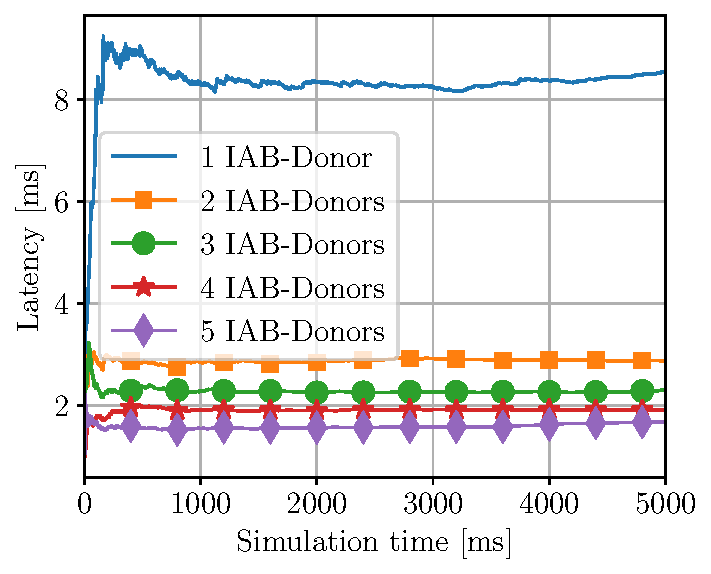
\includegraphics[width=.25\linewidth]{Figures/Safehaul/S3_lat.pdf}
    \label{fig:avgE2EDelay_s3}
    }
\subfloat[][Average per-UE throughput]{
    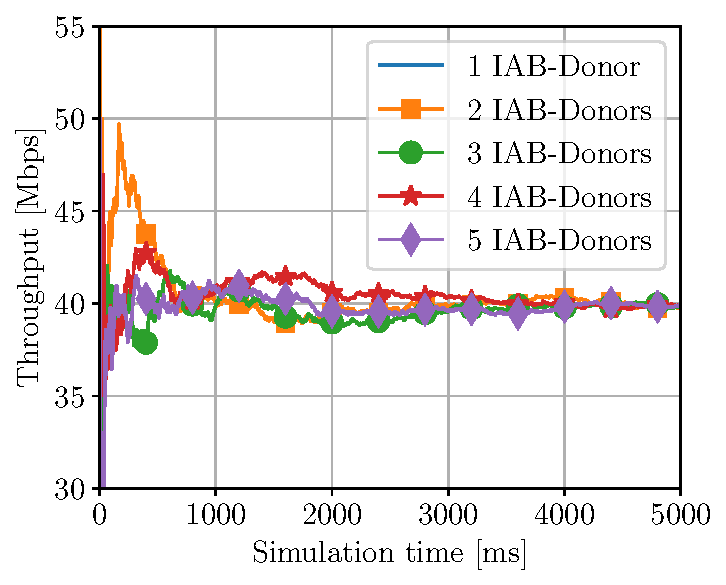
\includegraphics[width=.25\linewidth]{Figures/Safehaul/S3_thr.pdf}
    \label{fig:avgTput_s3}
    }
\subfloat[][Average per-UE packet drop rate]{
    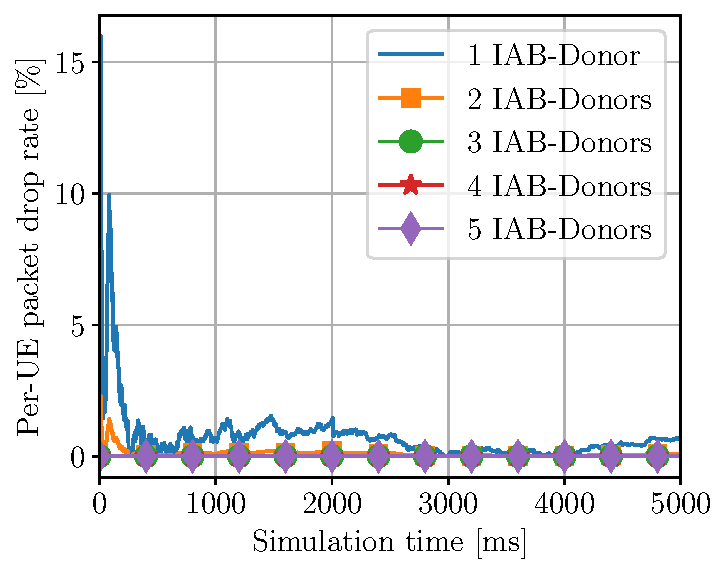
\includegraphics[width=.25\linewidth]{Figures/Safehaul/S3_drop.pdf}
    \label{fig:avgDropRate_s3}
    }
  
   \caption{Network performance for $50$ \glspl{ue} and $40$ Mbps per-UE source rate, versus the number of \donors{} (Scenario 3).}
  \label{fig:avgNetPerfomance_s3}
  \vspace*{-3mm}
\end{figure*}
We observe in Fig.~\ref{fig:avgE2EDelay_s3} that the highest latency is experienced when only one \donor{} is present in the network. This stems from the tributary effect of self-backhauling where the traffic flows towards a central entity which itself can become a bottleneck. As the number of \donors{} increases, the traffic is more evenly distributed, resulting in lower latency. Specifically, the average latency decreases from 8.2~ms for $D=1$ to 1.7~ms when $D=5$. As mentioned, since the load is constant in this scenario, the average throughput also remains constant for all different numbers of \donors{}, see Fig.~\ref{fig:avgTput_s3}. Notably, \name{}'s  learning speed is maintained for the different values of $D$.
This is an important design feature of \name{} because having more \donors{} means that the number of paths a \node{} has to the core network increases exponentially. From a learning perspective, such increment implies a larger action set and a lower learning speed. \name{} avoids this problem by learning the average latency based on the estimates of its neighbors and not on the complete paths to the \donors{}.
Finally, Fig. \ref{fig:avgDropRate_s3} shows that increasing the number of \donors~significantly reduces the packet drops, which also stems from a better distribution of traffic flows in the network, as observed in Fig.~\ref{fig:avgE2EDelay_s3}. 

\begin{figure}[ t!]
    \centering
    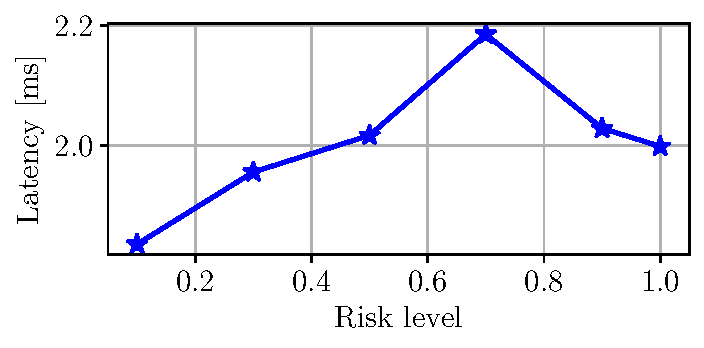
\includegraphics[width=0.6\columnwidth]{Figures/Safehaul/R_latency4.pdf}
    \setlength{\belowcaptionskip}{-12pt}
      \caption{Average latency for 50 UEs and 20 Mbps per-UE source rate, versus the risk level $\alpha$ (Scenario 4)}
      \label{fig:riskParam}
\end{figure}

\subsection{Scenario 4: Impact of the risk parameter $\alpha$}
The definition of losses in the tail of the latency distribution is controlled by the risk level parameter $\alpha$. Its impact on the average latency is shown in Fig. \ref{fig:riskParam}, where an increasing behavior is observed for $\alpha\leq 0.7$. The lowest latency is achieved for $\alpha=0.1$, which corresponds to the most risk-averse, and therefore the most reliable, case out of all the considered ones.
The non-monotonic behavior of the average latency versus $\alpha$ can be explained by the so-called exploration-exploitation trade-off: the higher $\alpha$, the higher the level of risk, which in turn leads \name{} to learn more about the environment and choose a more reliable action. Eventually, as $\alpha$ grows beyond approximately $0.7$, the performance of \name{} tends to that of the risk-neutral case. As a consequence, the algorithm undertakes excessive exploration, which causes a degradation of the average latency performance.


\begin{figure*}[t!]
\centering
\subfloat[][Average per-UE end-to-end latency]{
    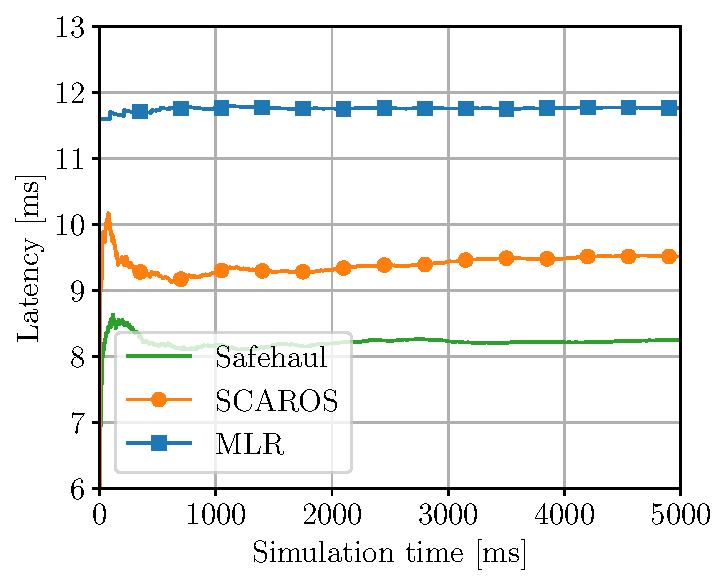
\includegraphics[width=.25\linewidth]{Figures/Safehaul/S1_lat_vs_time_padova.pdf}
    \label{fig:avgE2EDelayPadova}
    }
\subfloat[][Average per-UE throughput]{
    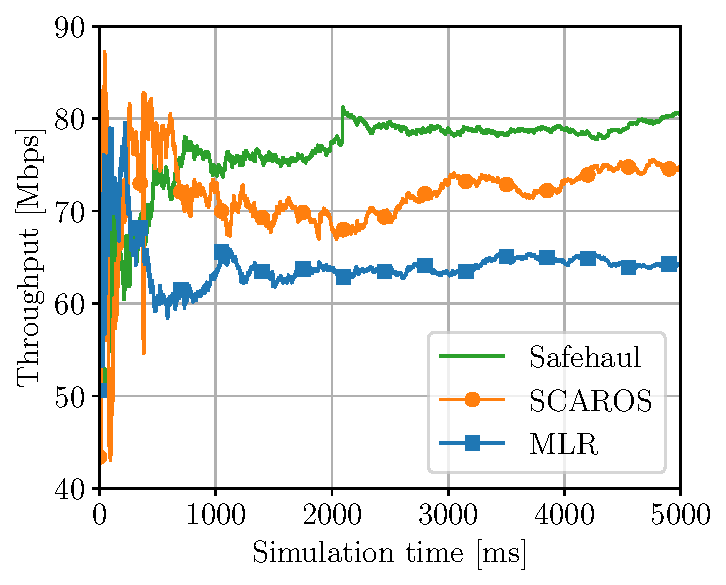
\includegraphics[width=.25\linewidth]{Figures/Safehaul/S1_thr_vs_time_padova.pdf}
    \label{fig:avgTputPadova}
    }
\subfloat[][Average per-UE packet drop rate]{
    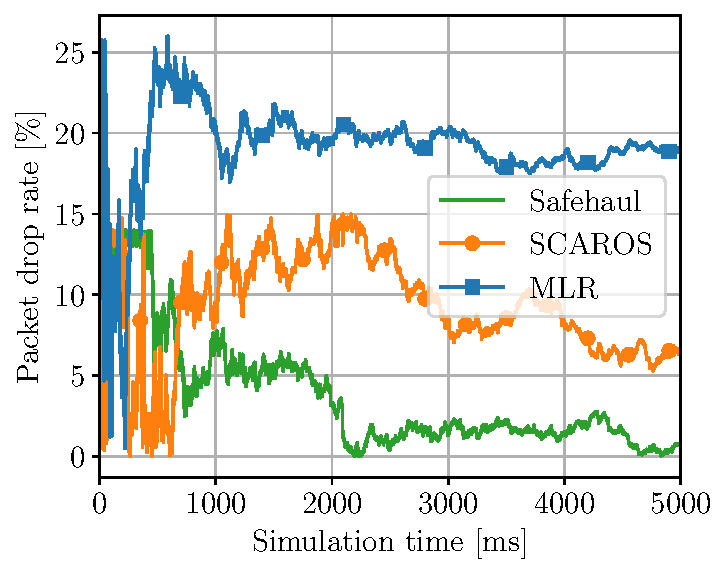
\includegraphics[width=.25\linewidth]{Figures/Safehaul/S1_drop_vs_time_padova.pdf}
    \label{fig:avgDropRatePadova}
    }
  
\caption{Average network performance for $50$ \glspl{ue} and $80$~Mbps per-UE source rate (Scenario 1) in Padova.}
  \label{fig:avgNetPerfomancePadova}
\end{figure*}



\begin{figure*}
\centering
\subfloat[][Per-UE end-to-end Latency]{
    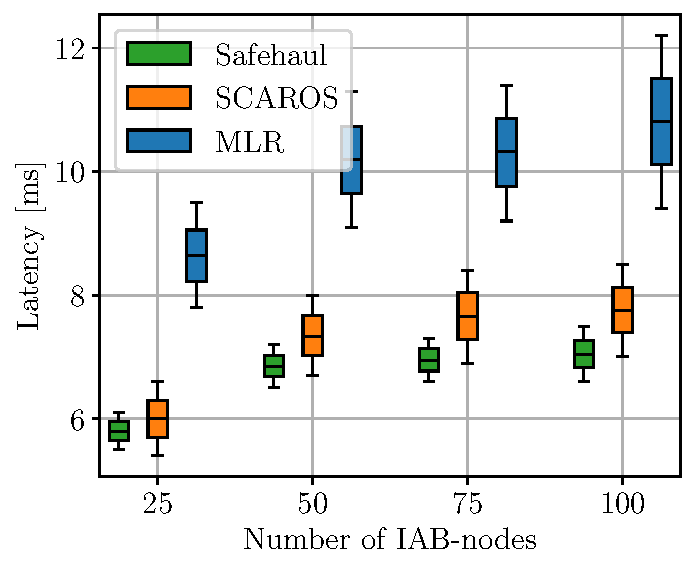
\includegraphics[width=.25\linewidth]{Figures/Safehaul/S2_lat_padova.pdf}
    \label{fig:avgE2EDelay_s2Padova}
    }
\subfloat[][Per-UE throughput]{
    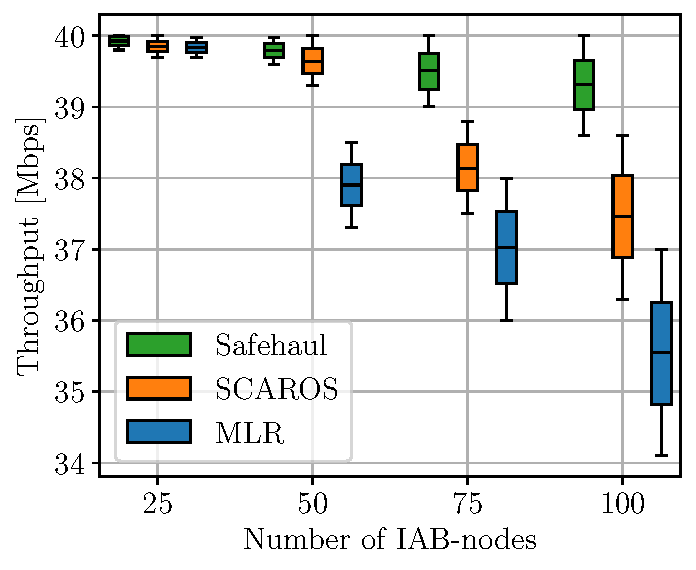
\includegraphics[width=.25\linewidth]{Figures/Safehaul/S2_thr_padova.pdf}
    \label{fig:avgTput_s2Padova}
    }
\subfloat[][Per-UE packet drop rate]{
    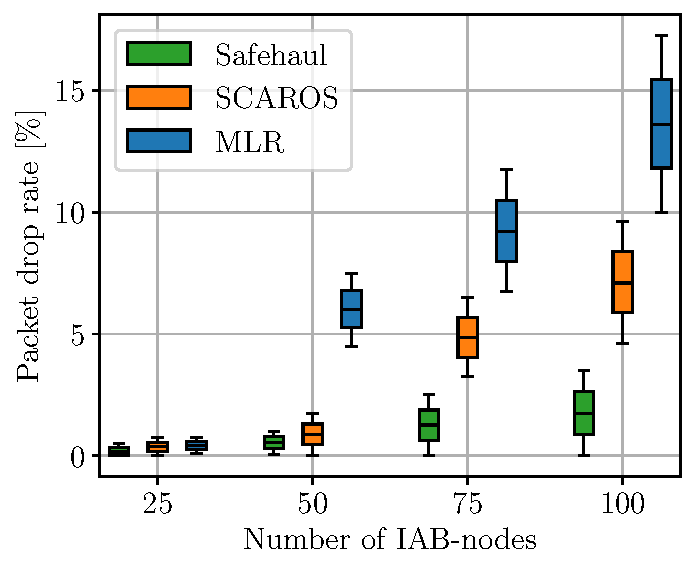
\includegraphics[width=.25\linewidth]{Figures/Safehaul/S2_drop_padova.pdf}
    \label{fig:avgDropRate_s2Padova}
    }
  
   \caption{Network performance for $\{25, 50, 75, 100\}$ \nodes{},$2$ UEs per \node{} on average, and $40$ Mbps per-UE source rate (Scenario 2) in Padova.}
  \label{fig:avgNetPerfomance_s2Padova}
  \vspace*{-3mm}
\end{figure*}

\begin{figure*}
\centering
\subfloat[][Average per-UE end-to-end Latency]{
    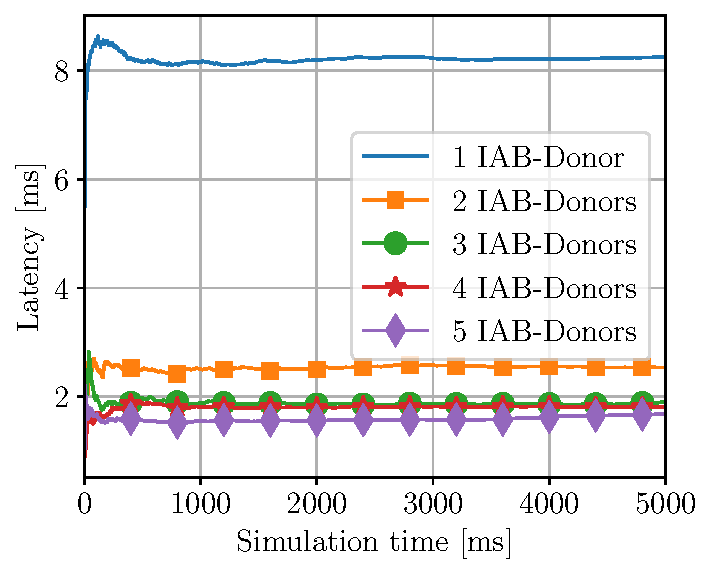
\includegraphics[width=.25\linewidth]{Figures/Safehaul/S3_lat_padova.pdf}
    \label{fig:avgE2EDelay_s3Padova}
    }
\subfloat[][Average per-UE throughput]{
    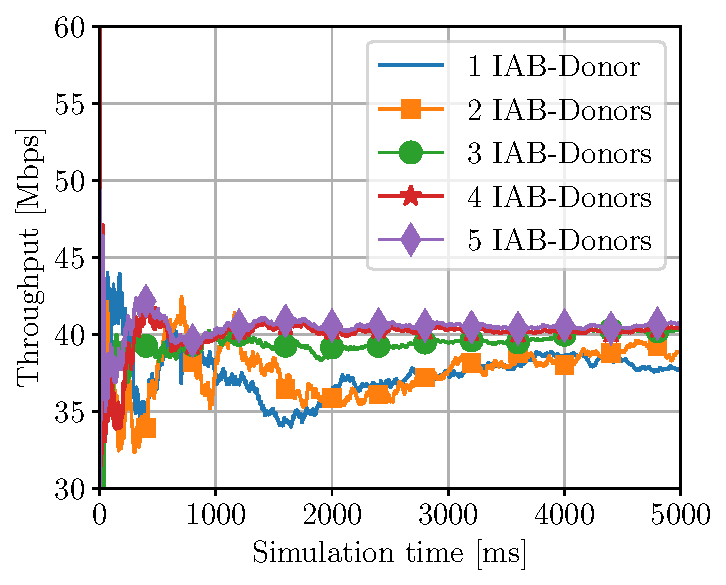
\includegraphics[width=.25\linewidth]{Figures/Safehaul/S3_thr_padova.pdf}
    \label{fig:avgTput_s3Padova}
    }
\subfloat[][Average per-UE packet drop rate]{
    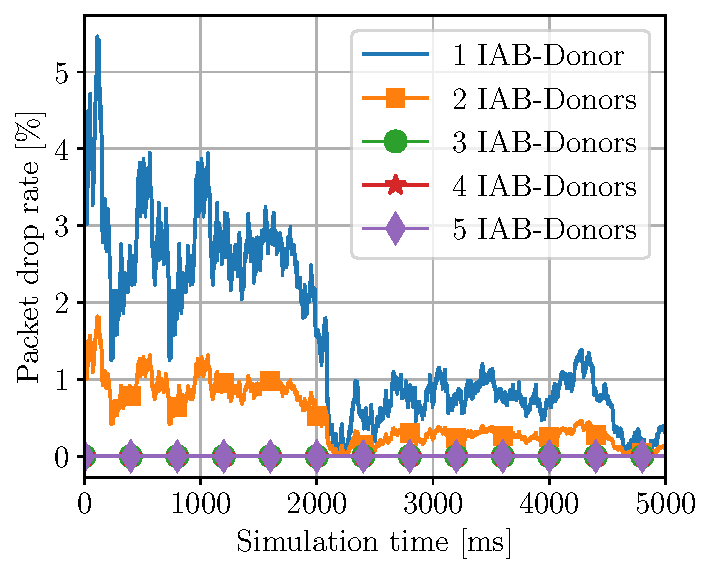
\includegraphics[width=.25\linewidth]{Figures/Safehaul/S3_drop_padova.pdf}
    \label{fig:avgDropRate_s3Padova}
    }
  
   \caption{Network performance for $50$ \glspl{ue} and $40$ Mbps per-UE source rate, versus the number of \donors{} in Padova (Scenario 3).}
  \label{fig:avgNetPerfomance_s3Padova}
  \vspace*{-3mm}
\end{figure*}

\subsection{Scenario 5: Performance in different topologies}


To verify the generality of the proposed algorithms, it is essential to examine how they perform in different topologies, and consider both typical network performance metrics (i.e., along the lines of Scenario 1) and their stability with respect to the number of \nodes{} and \donors{} (Scenarios 2 and 3). To this end, we ran additional simulations in the deployment depicted in Fig.~\ref{fig:Padova_Map}, which mimics the \nodes{} locations of the historic center of Padova. We report the average network performance over time, in terms of end-to-end packet drop rate, throughput, and latency in Fig.~\ref{fig:avgNetPerfomancePadova}. Overall, the outcomes of this simulation campaign are in line with those obtained in Scenario 1. 
Specifically, as seen in Fig.~\ref{fig:avgE2EDelayPadova}, \name{} quickly converges to an average latency of approximately 8~ms, which is 14\% and 31\% lower than SCAROS and MLR's latency. Fig.~\ref{fig:avgTputPadova} shows the average per-UE throughput, for which \name{} achieves about 4\% and 17\% better performance than SCAROS and MLR, respectively. Similarly, the performance depicted in Fig.~\ref{fig:avgDropRatePadova} is in line with that reported  in Figs.~\ref{fig:avgE2EDelayPadova} and ~\ref{fig:avgTputPadova}, with \name{} achieving approximately a 24\% and 38\% smaller packet drop rate than SCAROS and MLR, respectively. 

In Fig.~\ref{fig:avgNetPerfomance_s2Padova}, we compare the consistency of the performance of the three algorithms with respect to the network size. In particular, we change the number of \nodes{} from 25 to 100, keeping fixed the number of UEs per \node{} and thus effectively increasing the network load on the \donor{}. 
Results show that \name{}, when compared to other schemes, exhibits minimal performance degradation when introducing additional \nodes{} and \glspl{ue}. As can be seen in Fig.~\ref{fig:avgE2EDelay_s2Padova}, the latency achieved by \name{} increases by at most 16\% in the case of 100 \nodes{}, while SCAROS and MLR lead to a latency which is consistently higher and increases up to~27\% and ~25\% when deploying additional nodes, respectively.
Similar trends can be observed in Figs.~\ref{fig:avgTput_s2Padova} and \ref{fig:avgDropRate_s2Padova}, which report throughput and packet loss versus the network size, respectively. Indeed, \name{} is the best performer across the whole range of \nodes{} which have been considered. Furthermore, \name{} loses 20\% more packets with the denser network deployment (i.e., 100 \nodes{}), while reference schemes exhibit an increase in packet loss of up to 33\%. 

We complete this analysis by examining how the number of donors affects the performance achieved by \name{} in the Padova-like topology. 
As can be seen in Fig.~\ref{fig:avgNetPerfomance_s3Padova}, increasing the number of fiber-backhauled base stations progressively reduces the latency. Similarly, and in line with the results obtained in Scenario 3 and reported in Fig.~\ref{fig:avgDropRate_s3Padova}, the packet drop rate varies from approximately 0.08\% when considering a single \donor{}, to approximately 0.003\% in the presence of five \donors{}. The performance improvements introduced by additional fiber links saturate after 3 donors, thanks to the efficient routing and scheduling performed by \name{}.

In summary, the results obtained in the additional topology mimicking the historical center of Padova are well aligned with those obtained in the Manhattan topology. Although the specific values of the network metrics achieved by the considered schemes in the two topologies are different (for instance, SCAROS achieves a 66\% lower packet drop rate in Scenario~1 compared to Scenario~5), the trends among the various schemes are the same. Specifically, we observed that \name{} consistently achieves the best performance in comparison to SCAROS and MLR across different metrics, which supports the claim that the proposed scheduler is capable of learning how to optimize arbitrary deployment topologies.

\subsection{Scenario 6: Network resilience}
In networking, resilience refers to the ability of a network to recover in a quick and effective fashion from disruptions, thus providing reliable and high-quality communication services to its users.
Specifically, the ability to recover from link failures is particularly important in \gls{iab} networks, where backhaul links are susceptible to the typical disruptions which plague the \gls{ran} due to its mobile and wireless nature. For instance, the links among \nodes{} can be degraded by adverse environmental conditions such as heavy rain and monsoons, physical obstacles and network congestion. These disruptions can cause temporary or permanent communication failures, which in turn result in degraded performance and/or loss of connectivity for the end users. 
To prevent and/or recover from these undesired events, a backhaul scheduler must detect, mitigate, and recover from various types of disruptions and failures, and must maintain the required level of service availability and performance despite the time-varying channel conditions.

\begin{figure*}[t!]
\centering
\subfloat[][Average per-UE end-to-end latency]{
    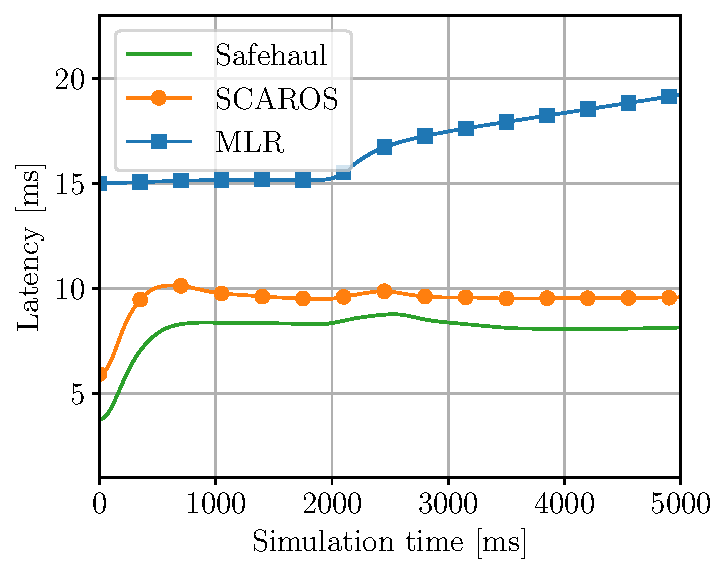
\includegraphics[width=.25\linewidth]{Figures/Safehaul/S6_lat_vs_time.pdf}
    \label{fig:avgE2EDelay_Re}
    }
\subfloat[][Average per-UE throughput]{
    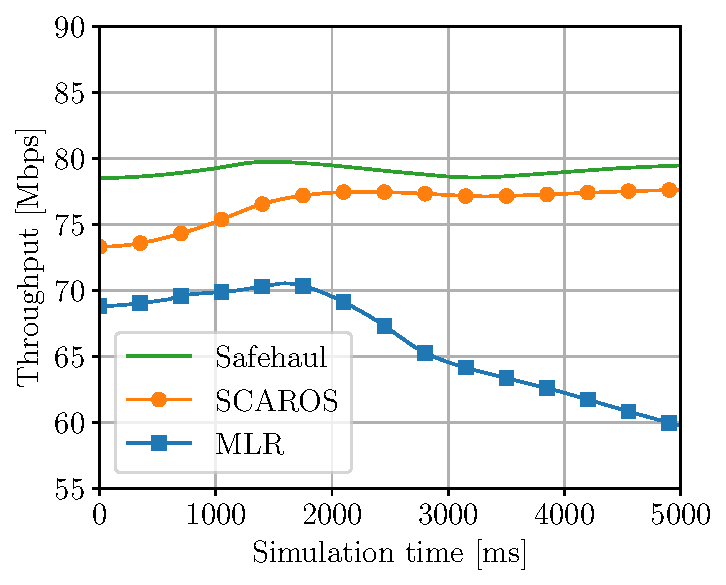
\includegraphics[width=.25\linewidth]{Figures/Safehaul/S6_thr_vs_time.pdf}
    \label{fig:avgTput_Re}
    }
\subfloat[][Average per-UE packet drop rate]{
    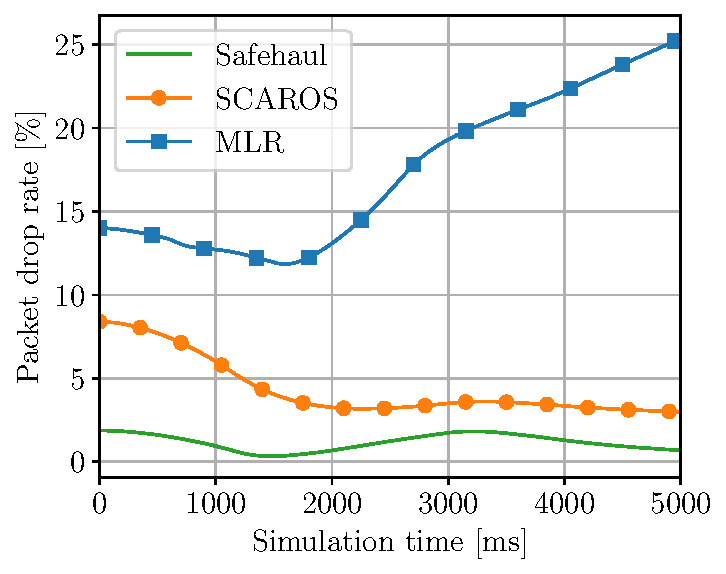
\includegraphics[width=.25\linewidth]{Figures/Safehaul/S6_drop_vs_time.pdf}
    \label{fig:avgDropRate_Re}
    }
  
\caption{Average network performance for $50$ \glspl{ue} and $80$~Mbps per-UE source rate where 1 random \node{} is shut down.}
  \label{fig:avgNetPerfomance_Re}
\end{figure*}


\begin{figure*}[t!]
\centering
\subfloat[][Average per-UE end-to-end latency]{
    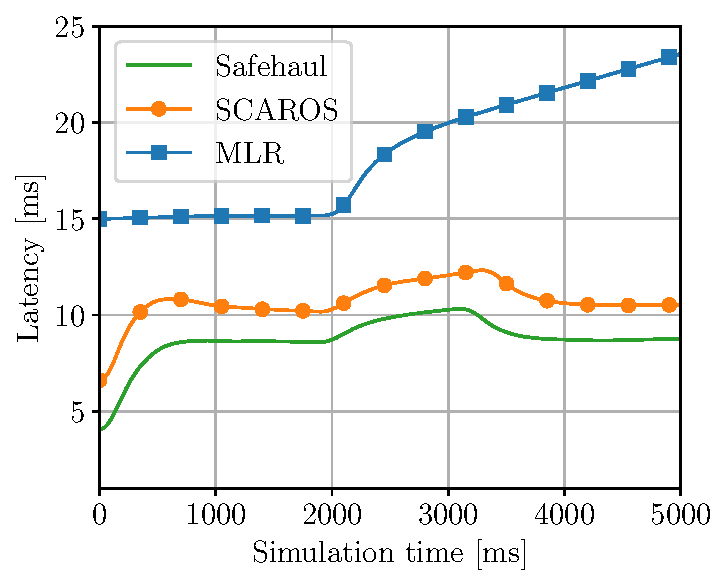
\includegraphics[width=.25\linewidth]{Figures/Safehaul/S7_lat_vs_time.pdf}
    \label{fig:avgE2EDelay_Re2}
    }
\subfloat[][Average per-UE throughput]{
    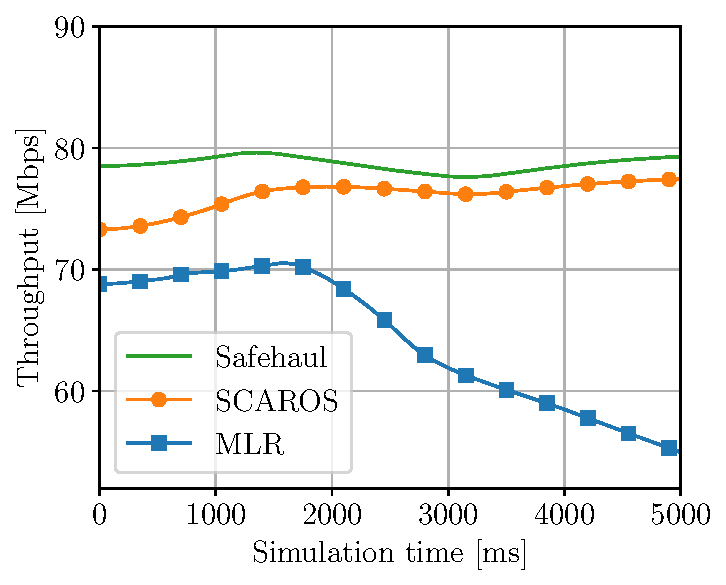
\includegraphics[width=.25\linewidth]{Figures/Safehaul/S7_thr_vs_time.pdf}
    \label{fig:avgTput_Re2}
    }
\subfloat[][Average per-UE packet drop rate]{
    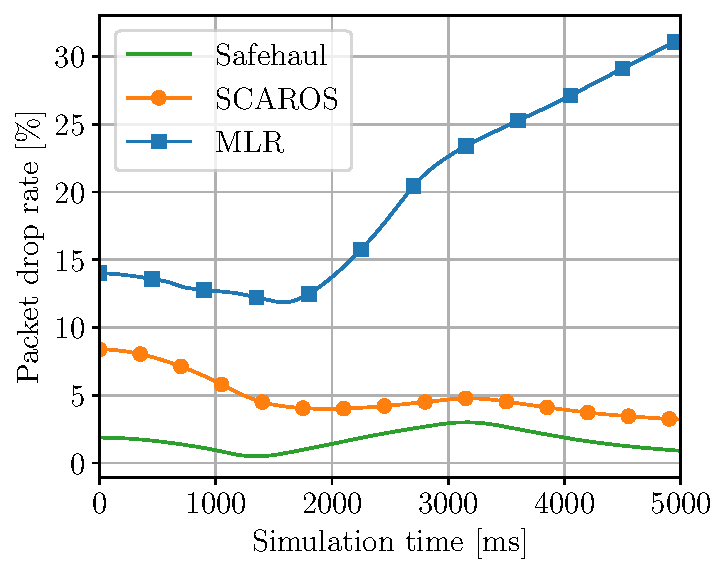
\includegraphics[width=.25\linewidth]{Figures/Safehaul/S7_drop_vs_time.pdf}
    \label{fig:avgDropRate_Re2}
    }
  
\caption{Average network performance for $50$ \glspl{ue} and $80$~Mbps per-UE source rate where 3 random \nodes{} are shut down.}
  \label{fig:avgNetPerfomance_Re2}
\end{figure*}

We benchmark the resilience of the proposed algorithm by mimicking radio link failures, which we simulate by stopping \nodes{} at a fixed time instant (2000~s), and inspecting the resulting performance degradation.
Since the failed node(s) is (are) chosen at random, we run multiple simulations to estimate the average network performance, as shown in Figs.~\ref{fig:avgNetPerfomance_Re} and~\ref{fig:avgNetPerfomance_Re2} for the case of one and three link failures, respectively.

Results show that MLR is unable to react to the link failure(s) due to its static and myopic policy. Specifically, the disruption causes an increase of~33\% (60\%) in latency, and a decrease of up to 15\% (23\%) in throughput when considering one (three) link failure(s).
On the other hand, both \name{} and SCAROS are capable of adapting the scheduling to the new topology. Indeed, both schemes show a transient region where the performance is slightly degraded since the algorithms are learning new routes and resource partitions to account for the lost link. Nevertheless, \name{} and SCAROS eventually converge to a solution which provides approximately the same network performance as before the failures, in both cases of one and three lost links.

\section {Related work}
\label{s:related}

Self-backhauling wireless networks have been studied in different contexts. Ranging from the so-called \glspl{hetnet} and \gls{iab} 5G \gls{nr} systems, to \glspl{cran}, each has considered a different set of premises and optimization goals. In this section, we review the related work in the context of basic assumptions and their optimization goals. 

\textbf{Ideal backhaul links.} Numerous works assume either an \textit{infinite or fixed capacity backhaul link}. This is often motivated by the presence of a wired fiber link between the \glspl{sbs} and the \gls{mbs}~\cite{pan2017joint, huang2015joint, nguyen2020nonsmooth, rasekh2015interference}. Indeed, most of these works consider a scenario where a centralized \gls{bbu} is connected to several \glspl{rrh}, i.e., radios which lack signal processing capabilities~\cite{pan2017joint, huang2015joint, nguyen2020nonsmooth}. In particular, the authors of~\cite{nguyen2020nonsmooth} consider an even more complex C-RAN scenario where RRHs feature caching and signal processing capabilities. However, in an \gls{iab} context it is fundamental to consider \textit{limited-rate, time-varying backhaul channels} and to study the impact of such limitations on the performance of the \gls{ran}.

\textbf{Constrained topologies.} It is often assumed that self-backhauled networks have a \textit{specific topology}. This assumption usually simplifies the problem and makes it tractable and/or solvable in polynomial time. For instance, the authors of~\cite{kwon2019joint, pizzo2017optimal, lei2020deep} assume a single-hop network where each \gls{sbs} is directly connected to the \gls{mbs}. In~\cite{kulkarni2018max}, a $k$-ring deployment is considered, i.e., a topology where a single \gls{iab}-donor provides backhaul connectivity to $k$ rings of \gls{iab}-nodes. Even though this topology can be used to model networks with arbitrary depth, it maintains a symmetric load for each node, an assumption which generally does not hold in real networks.
In fact, the 3GPP does not impose any limits on the number of \gls{iab}-nodes which can be connected to a given \gls{iab}-donor, nor does it set an upper bound on the number of wireless hops from the latter to other wireless-backhauled base stations~\cite{3gpp_38_874}. Accordingly, in our problem formulation we consider \gls{iab} networks with an \textit{arbitrary number of nodes and an arbitrary maximum number of wireless hops} between \glspl{mbs} and \glspl{sbs}. 

\textbf{Simplistic traffic models.} Some works either assume a \textit{full buffer traffic model and/or impose flow conservation constraints}. In particular, the authors of~\cite{yuan2018optimal, rasekh2015interference} consider systems where the capacity of each link can  always be fully exploited thanks to the presence of \textit{infinite data to transmit at each node}. However, in actual \gls{iab} deployments the presence of packets at the \glspl{mbs} and \glspl{sbs} is conditioned on the \textit{status of their \gls{rlc} buffers and, in turn, on the previous scheduling decisions}. Moreover, \textit{packets can actually be buffered at the intermediate nodes}, thus preventing the need for transmitting a given packet in consecutive time instants along the whole route from the \gls{iab}-donor to the \glspl{ue} (or vice versa). 

\textbf{Optimization goals.} The works in the literature focus on different optimization goals. Therefore, they prioritize different network metrics. For instance, the authors of~\cite{hur2013millimeter} aim to optimize the beam alignment between \glspl{mbs} and \glspl{sbs}. Instead, the work of~\cite{alizadeh2019load} aims to compute the optimal user-to-base-station association. However, they neglect backhaul associations and focus on the access only. In~\cite{kwon2019joint, alizadeh2019load, zhu2016qos, yuan2018optimal} the objective function is a function of the users data-rate. In particular, the authors of~\cite{yuan2018optimal} optimize the max-min user throughput, arguing that such a metric better captures the performance of the bottleneck links. In~\cite{vu2018path}, the average rate of each link is maximized under bounded delay constraints. In our work, we focus on reliability by minimizing not only the average end-to-end delay, but also the expected value of the worst-case performance.
The work closest to this article is SCAROS~\cite{ortiz2019scaros},  a learning-based latency-aware scheme for resource allocation and path selection in self-backhauled networks. Assuming a single IAB-donor, the authors study arbitrary multi-tier \gls{iab} networks considering the impact of interference and network dynamics. In contrast, we aim at enhancing the reliability of the IAB-network by jointly minimizing the average end-to-end delay and its expected tail loss. 

\section{Conclusion}
\label{s:conclusion}
In this work, we proposed the first reliability-focused scheduling and path selection algorithm for \gls{iab} mmWave networks. We illustrated that our \gls{rl}-based solution can cope with the network dynamics including channel, interference, and load.  Furthermore, we demonstrated that \name{} not only  exhibits highly reliable performance in the presence of the above-mentioned network dynamics, but also outperforms the benchmark schemes in terms of throughput, latency and packet-drop rate. The reliability of \name{} stems from the joint minimization of the average latency, and the expected value of its tail losses, by leveraging \gls{cvar} as a risk metric.

Reliability is a highly under-explored topic that definitely deserves more investigation. Some interesting research directions are the maximization of reliability under the assumption of statistical system knowledge, or the evaluation of the network's reliability when the functionality of the \gls{bap} layer is compromised.
Furthermore, our system-level extension to Sionna can be further developed to support an arbitrary number of RF chains and in-band backhauling, allowing more extensive investigation of IAB protocols and architectures.

\section*{Appendix}
\label{sec:appendix}
For the proof of Proposition \ref{prop:probNonOptArm}, Theorem 3 in \cite{Luo2017} is needed. For completeness, we first present the theorem in \cite{Luo2017} for the special case in which the considered random variables are independent. Next, we present the proof of Proposition \ref{prop:probNonOptArm}.
\begin{theorem} \label{eq:Theorem2_part2}
Let $T_{a_n,i}$ be independent random variables where $\max_{1\leq j\leq i}{T_{a_n,j}} = T_\mathrm{max}$, with $i\in\{1,2,...\}$.
Then, for any $0 < \delta \leq 1/2$, $\xi > 0$ and $\gamma > 0$, there exists a positive constant $C$ which only depends on $\xi$ and $\gamma$, such that the probability of the event $|\estcvar{a_n,i}-\cvar{a_n,i}| \geq 2\xi\alpha^{-1}T_{\max} i^{-\delta}(\ln{\ln{i}})^{1/2}\ln{i}$ is smaller than or equal to $Ce^{-(1+\gamma)\ln i}$.
\end{theorem}
\begin{proof}
See Theorem 3 in \cite{Luo2017}.
\end{proof}

\subsection*{Proof of Proposition \ref{prop:probNonOptArm}}
\begin{proof}[\unskip\nopunct]

In this proof, we use the result of the regret bound for the risk-neutral case without CVaR, shown in \cite[Theorem 3]{Auer2002}, as a basis. Additionally, we use the bound for the terms related to the CVaR formulated in \cite[Theorem 3]{Luo2017}. 
Using both these results, we first bound the probability that Safehaul chooses a suboptimal arm in the exploitation phase. Then, we combine the latter with the probability of choosing a suboptimal arm in the exploration phase to derive the bound given in Proposition~\ref{prop:probNonOptArm}.

From the system model and Proposition \ref{prop:probNonOptArm}, we have that $c > 0$, $0 < d \leq 1$, and 
$\epsilon_n := \min(1, \frac{cA_n}{d^2i})$. 
Moreover, $a_{n,i}$ is the action chosen by $\epsilon$-greedy in time slot $i$ and $K_{a_n, i}$ is the number of times, up to time slot $i$, in which \name{} chose action $a_n$ \textit{at random}. Similarly, we use $K^*_{i}$ for the counter of the optimal action.
$T_{a_n, i}$ are independent random variables distributed according to the rewards linked to action $a_n$. We use $T_i^*$ for the optimal action, and $\hat{T}_{a_n, i}$ is the estimated mean of the probability distribution of the rewards linked to action $a_n$ using $K_{a_n,i}$ samples. As before, we use $\hat{T}^*_{i}$ for the optimal action.
$\estcvar{a_n, i}$ is the estimated \gls{cvar} of action $a_n$ up to time slot $i$ and $\estcvar{i}^*$ is the estimated \gls{cvar} of the optimal action up to time slot $i$.
Then, the probability that action $a_n$ is chosen in time slot $i$ is upper bounded as
{\small
 \begin{align}
     \label{eq:inicProbAction}
    \mathbb{P}[a_{n,i} = a_n] \leq & \mathbb{P}\left[\delta_{a_n,i-1} \leq \delta_{i-1}^* \right]\left(1 - \frac{\epsilon_i}{A_n} \right) + \frac{\epsilon_i}{A_n},
\end{align} }
 with $\delta_{a_n,i-1} = \hat{T}_{a_n, i-1} + \eta \estcvar{a_n, i-1}$ and $\delta^*_{i-1} = \hat{T}^*_{i-1} + \eta \estcvar{i-1}^*$.
The first term in \eqref{eq:inicProbAction} is the probability of exploitation and the second term to the probability of exploration. \\ 
Using the mean $\Bar{T}_{a_n}$ and $\cvar{a_n}$ of action $a_n$, and the likewise defined $\Bar{T}^*$ and $\cvar{}^*$ for the optimal action, we set $\Delta^\mathrm{mean}_{a_{n}} := \Bar{T}_{a_n} - \Bar{T}^*$ and $\Delta^\mathrm{cvar}_{a_{n}} := \cvar{a_n} - \cvar{}^*$.
Using these definitions in \eqref{eq:inicProbAction} we conclude
{\small
\begin{align}
    \mathbb{P} &\left[\delta_{a_n,i-1} \leq \delta_{i-1}^*\right] \leq \nonumber \\
    &\mathbb{P}\!\left[\delta_{a_n,i-1} \leq \eta \cvar{a_n}  - \frac{\Delta^\mathrm{mean}_{a_n}}{2} + \right. \left. \bar{T}_{a_n}  - \eta \frac{\Delta^\mathrm{cvar}_{a_n}}{2}\right] +\nonumber \\
    &\mathbb{P}\!\left[\bar{T}^* + \frac{\Delta^\mathrm{mean}_{a_n}}{2} + \eta \cvar{}^* +  \eta \frac{\Delta^\mathrm{cvar}_{a_n}}{2} \leq \delta_{i-1}^*\right] \nonumber \\
     & \mathbb{P}\!\left[\hat{T}_{a_n,i-1} \leq \bar{T}_{a_n} - \frac{\Delta^\mathrm{mean}_{a_n}}{2}\right] + \mathbb{P}\!\left[\bar{T}^* + \frac{\Delta^\mathrm{mean}_{a_n}}{2} \leq \hat{T}^*_{i-1}\right] + \nonumber \\
    &\mathbb{P}\!\left[\estcvar{a_n,i-1} \leq \cvar{a_n} - \frac{\Delta^\mathrm{cvar}_{a_n}}{2}\right]+ \nonumber \\
    & \mathbb{P}\!\left[\cvar{}^* + \frac{\Delta^\mathrm{cvar}_{a_n}}{2} \leq \estcvar{i-1}^*\right]. \label{eq:probBrokenDown}
\end{align}
}
Similar to \cite{Auer2002}, we use the Chernoff-Hoeffding bound for the first two terms in \eqref{eq:probBrokenDown}. For the last two  summands, there remains to find a bound for the difference between the \gls{cvar} and its estimate $\estcvar{}$. 
From Theorem \ref{eq:Theorem2_part2}, we set $\xi := {\Delta^\mathrm{cvar}_{a_n} \alpha}/{4 T_{max}}$, $\delta=0.5$ and by using the limit $\gamma \rightarrow 0$, we obtain
{\small
\begin{equation}
\begin{gathered}
    \mathbb{P}\!\left[|\estcvar{a_n,i}-\cvar{a_n,i}|\geq \frac{\Delta^\mathrm{cvar}_{a_n}}{2}i^{-0.5}(\ln{\ln{i}})^{0.5}\ln{i}\right] \leq \frac{C}{i}.
\end{gathered}
\end{equation}
}
As $\max_i i^{-0.5}(\ln{\ln{i}})^{0.5}\ln{i} < 1$, the condition ${(\Delta^\mathrm{cvar}_{a_n}}/{2})i^{-0.5}(\ln{\ln{i}})^{0.5}\ln{i} \leq \frac{\Delta^\mathrm{cvar}_{a_n}}{2}$
holds for all $i$. Therefore, considering the last two summands in \eqref{eq:probBrokenDown}, we conclude that there exists a positive constant $C$ that satisfies
{\small
\begin{equation}
\mathbb{P}\!\left[|\estcvar{a_n,i}-\cvar{a_n,i}|\geq \frac{\Delta^\mathrm{cvar}_{a_n}}{2}\right] \leq \frac{C}{i}.
\label{eq:partialCVaRBound}
\end{equation}}
The number of times action $a_n$ has been selected up to time slot $i$ is smaller than or equal to $i$, i.e., $K_{a_n,i}\leq i$. Using \eqref{eq:partialCVaRBound} we write the last two summands in \eqref{eq:probBrokenDown} as 
{\small
\begin{align}
    \mathbb{P}\!\left[\estcvar{a_n,i-1} \leq \cvar{a_n} - \frac{\Delta^\mathrm{cvar}_{a_n}}{2} \right] \leq \frac{C}{K_{a_n,i-1}},
\end{align}}
and
{\small
\begin{align}
    \mathbb{P}\!\left[\cvar{}^* + \frac{\Delta^\mathrm{cvar}_{a_n}}{2} \leq \estcvar{i-1}^*\right] \leq \frac{C}{K^*_{i-1}}.
\end{align}}
As in \cite{Auer2002}, we use Bernstein's inequality to get an estimate for $K_{a_n,i-1}$. Defining $x_0 := {1}/{2A_n}\sum_{j=1}^{i-1}\epsilon_j$ for $i-1 \geq \frac{cA_n}{d^2}$ we get $P(K_{a_n,i-1} \leq x_0) \leq e^{-\frac{x_0}{5}}$.
Additionally, from \cite{Auer2002}: 
{\small
\begin{equation}
    x_0 \geq \frac{c}{d^2}\ln\left(\frac{(i-1)d^2e^{0.5}}{cA_n}\right) =: C'(i).
\end{equation}}
The same holds for the optimal action and $K^*_{i-1}$. Using these estimations for $x_0$, we can conclude that for $i-1 \geq {cA_n}/{d^2}$
{\small
\begin{align}
    &\mathbb{P}\!\left[\estcvar{a_n,i-1} \leq \cvar{a_n} - \frac{\Delta^\mathrm{cvar}_{a_n}}{2}\right] \\
    &\leq \sum_{j=1}^{i-1} \mathbb{P}[K_{a_n,i-1}=j] \frac{C}{j} \nonumber \\
    &= \sum_{j=1}^{\lfloor x_0 \rfloor} \mathbb{P}[K_{a_n,i-1}=j] \frac{C}{j} + \sum_{j=\lfloor x_0 \rfloor + 1}^{i-1} \mathbb{P}[K_{a_n,i-1}=j] \frac{C}{j} \nonumber\\
    &\leq C x_0 e^{-\frac{x_0}{5}} + \frac{C}{x_0} \leq C x_0 e^{-\frac{x_0}{5}} + \frac{C}{C'(i)}.
\end{align}
}
The same holds again for the optimal action
{\small
\begin{align}
    \mathbb{P}\!\left[\cvar{}^* + \frac{\Delta^\mathrm{cvar}_{a_n}}{2} \leq \estcvar{i-1}^*\right] &\leq C x_0 e^{-\frac{x_0}{5}} + \frac{C}{C'(i)}.
\end{align}}
Together with the bounds from Theorem 3 in \cite{Auer2002} it follows that for $C \geq 1$:
{\small
\begin{align*}
    \mathbb{P}&\left[a_{n,i} = a_n\right] \\
    &\leq \frac{\epsilon_i}{A_n} + 4 C x_0 e^{-\frac{x_0}{5}} + \frac{4}{\left(\Delta^\mathrm{mean}_{a_n}\right)^2}e^{\frac{-\left(\Delta^\mathrm{mean}_{a_n}\right)^2\lfloor x_0 \rfloor}{2}}  + 2 \frac{C}{C'(n)} \nonumber \\
    &\leq \frac{c}{d^2i} +  2 \frac{Cd^2}{c\ln\left(\frac{(i-1)d^2e^{0.5}}{cA_n}\right)}
    + \frac{4e}{d^2}\left(\frac{c A_n}{(i-1)d^2e^{0.5}}\right)^{\frac{c}{2}} +\\
    & \:\:\quad 4C\frac{c}{d^2}\ln\left(\frac{(i-1)d^2e^{0.5}}{c A_n}\right) \left(\frac{c A_n}{(i-1)d^2e^{0.5}}\right)^{\frac{c}{5d^2}}.
\end{align*}
}
\end{proof}
  %%%%%%%%%%%%
%%% WONS %%%
%%%%%%%%%%%%


% \documentclass[a4paper, conference]{IEEEtran}
% \IEEEoverridecommandlockouts

% \pagestyle{empty}
% \usepackage{url}
% \usepackage[utf8]{inputenc}
% \usepackage{xcolor}
% \usepackage{amsmath}
% \usepackage{amssymb}
%\usepackage{algorithm}
%\usepackage{algorithmic}
\newcommand{\red}[1]{\begin{color}{red}#1\end{color}}

%\usepackage{geometry}
%\geometry{letterpaper, margin=1.3in}

% \usepackage[bottom=4.0cm, left=1.57cm, right=1.57cm, top=1.75cm]{geometry}

% \usepackage[acronyms,nonumberlist,nopostdot,nomain,nogroupskip]{glossaries}
% \usepackage{tablefootnote}
% \usepackage{booktabs}
% \usepackage{tabularx}
% \usepackage{tikz}
% \usepackage{pgfplots}
% \pgfplotsset{compat=newest}
% \pgfplotsset{plot coordinates/math parser=false}
% \usepackage{soul}
% \newlength\fheight
% \newlength\fwidth
% \usetikzlibrary{plotmarks,patterns, patterns.meta,decorations.pathreplacing,backgrounds,calc,arrows,arrows.meta,spy,matrix,backgrounds}
% \usepgfplotslibrary{patchplots,groupplots}
% \usepackage{tikzscale}
% \usepackage{hyperref}
% \usepackage{algorithm} 
% \usepackage{algpseudocode} 
% \usepackage{comment}
% \usepackage{bm}
% \usepackage{multirow}
% \usepackage{bbm}

% \renewcommand{\figurename}{Fig.}
% %\renewcommand{\tablename}{Tab.}
% \usepackage[font=small]{subcaption}
% \usepackage[font=small]{caption}

%\usepackage{mathtools}

% \newcommand{\MP}[1]{\color{red}{\textbf{TODO: #1 }}\color{black}}

%\usepackage{dblfloatfix}    % To enable Figures/IabThzLinks at the bottom of page
% \usepackage{colortbl}

%\usepackage{cite}

%\newacronym{3gpp}{3GPP}{3rd Generation Partnership Project}
\newacronym{adc}{ADC}{Analog to Digital Converter}
\newacronym{afbw}{AFBW}{Average Fading Bandwidth}
\newacronym{5g}{5G}{5th generation}
\newacronym{4g}{4G}{4th generation}
\newacronym{aimd}{AIMD}{Additive Increase Multiplicative Decrease}
\newacronym{am}{AM}{Acknowledged Mode}
\newacronym{amf}{AMF}{Access and Mobility Management Function}
\newacronym{an}{AN}{Access Network}
\newacronym{amc}{AMC}{Adaptive Modulation and Coding}
\newacronym{aqm}{AQM}{Active Queue Management}
\newacronym{awgn}{AGWN}{Additive White Gaussian Noise}
\newacronym{balia}{BALIA}{Balanced Link Adaptation}
\newacronym{bsr}{BSR}{Buffer Status Report}
\newacronym{msr}{MSR}{Max Sum-Rate}
\newacronym{ba}{BA}{Backlog Avoidance}
\newacronym{mrba}{MRBA}{Max-Rate Backlog Avoidance}
\newacronym{bdp}{BDP}{Bandwidth-Delay Product}
\newacronym{bf}{BF}{Beamforming}
\newacronym{v2x}{V2X}{Vehicle-to-Everything}
\newacronym{vr}{VR}{Virtual Reality}
\newacronym{mdp}{MDP}{Markov Decision Process}
\newacronym{mwm}{MWM}{Maximum Weighted Matching}
\newacronym{tdm}{TDM}{Time Division Multiplexing}
\newacronym{fdm}{FDM}{Frequency Division Multiplexing}
\newacronym{sdm}{SDM}{Space Division Multiplexing}
\newacronym{st}{ST}{Spanning Tree}
\newacronym{rl}{RL}{Reinforcement Learning}
\newacronym{lp}{LP}{Linear Programming}
\newacronym[firstplural=Deep Neural Networks (DNNs)]{dnn}{DNN}{Deep Neural Network}
\newacronym{dag}{DAG}{Directed Acyclic Graph}
\newacronym{gtp}{GTP}{GPRS Tunneling Protocol}
\newacronym{nas}{NAS}{Non-Access Stratum}
\newacronym{isp}{ISP}{Internet Service Provider}
\newacronym{ngnm}{NGNM}{Next Generation Mobile Networks Alliance}
\newacronym{cc}{CC}{Component Carrier}
\newacronym{drb}{DRB}{Data Radio Bearer}
\newacronym{qos}{QoS}{Quality of Service}
\newacronym{ca}{CA}{Carrier Aggregation}
\newacronym{sdap}{SDAP}{Service Data Adaptation Protocol}
\newacronym{lc}{LC}{Logical Channel}
\newacronym{rnti}{RNTI}{Radio Network Temporary Identifier}
\newacronym{qci}{QCI}{Quality Class Identifier}
\newacronym{cdf}{CDF}{Cumulative Distribution Function}
\newacronym{cmos}{CMOS}{Complementary Metal-Oxide Semiconductor}
\newacronym{cn}{CN}{Core Network}
\newacronym{cqi}{CQI}{Channel Quality Information}
\newacronym{cir}{CIR}{Channel Impulse Response}
\newacronym{cp}{CP}{Control Plane}
\newacronym{cu}{CU}{Central Unit}
\newacronym{du}{DU}{Distributed Unit}
\newacronym{csirs}{CSI-RS}{Channel State Information - Reference Signal}
\newacronym{dc}{DC}{Dual Connectivity}
\newacronym{imsi}{IMSI}{International Mobile Subscriber Identity}
\newacronym{dce}{DCE}{Direct Code Execution}
\newacronym{dci}{DCI}{Downlink Control Information}
\newacronym{uci}{UCI}{Uplink Control Information}
\newacronym{dl}{DL}{Downlink}
\newacronym{dmr}{DMR}{Deadline Miss Ratio}
\newacronym{dmrs}{DMRS}{DeModulation Reference Signal}
\newacronym{e2e}{E2E}{End-to-End}
\newacronym{ecn}{ECN}{Explicit Congestion Notification}
\newacronym{edf}{EDF}{Earliest Deadline First}
\newacronym{enb}{eNB}{evolved Node Base}
\newacronym{embb}{eMBB}{enhanced Mobile Broadband}
\newacronym{epc}{EPC}{Evolved Packet Core}
\newacronym{es}{ES}{Edge Server}
\newacronym{fdma}{FDMA}{Frequency Division Multiple Access}
\newacronym{fdd}{FDD}{Frequency Division Duplexing}
\newacronym[firstplural=Radio Access Technologies (RATs)]{rat}{RAT}{Radio Access Technology}
\newacronym[firstplural=Markov Chains (MCs)]{mc}{MC}{Markov Chain}
\newacronym{milp}{MILP}{Mixed-Integer Linear Programming}
\newacronym{fs}{FS}{Fast Switching}
\newacronym{ip}{IP}{Internet Protocol}
\newacronym{fr}{FR}{Frequency Range}
\newacronym{ftp}{FTP}{File Transfer Protocol}
\newacronym{gnb}{gNB}{Next Generation Node Base}
\newacronym{arq}{ARQ}{Automatic Repeat reQuest}
\newacronym{harq}{HARQ}{Hybrid Automatic Repeat reQuest}
\newacronym{hetnet}{HetNet}{Heterogeneous Network}
\newacronym{hh}{HH}{Hard Handover}
\newacronym{hol}{HOL}{Head-of-Line}
\newacronym{ia}{IA}{Initial Access}
\newacronym{imt}{IMT}{International Mobile Telecommunication}
\newacronym{iot}{IoT}{Internet of Things}
\newacronym{lcr}{LCR}{Level Crossing Rate}
\newacronym{lcf}{LCF}{Level Crossing Frequency}
\newacronym{los}{LoS}{Line-of-Sight}
\newacronym{lte}{LTE}{Long Term Evolution}
\newacronym{m2m}{M2M}{Machine to Machine}
\newacronym{mac}{MAC}{Medium Access Control}
\newacronym{num}{NUM}{Network Utility Maximization}
\newacronym{ri}{RI}{Rank Index}
\newacronym{pmi}{PMI}{Precoding Matrix Index}
\newacronym{mcs}{MCS}{Modulation and Coding Scheme}
\newacronym{mec}{MEC}{Mobile Edge Cloud}
\newacronym{mi}{MI}{Mutual Information}
\newacronym{mimo}{MIMO}{Multiple Input, Multiple Output}
\newacronym{mmwave}{mmWave}{millimeter wave}
\newacronym{mptcp}{MPTCP}{Multipath TCP}
\newacronym{mr}{MR}{Maximum Rate}
\newacronym{mt}{MT}{Mobile Termination}
\newacronym{mss}{MSS}{Maximum Segment Size}
\newacronym{mtd}{MTD}{Machine-Type Device}
\newacronym{mtu}{MTU}{Maximum Transmission Unit}
\newacronym{nfv}{NFV}{Network Function Virtualization}
\newacronym{nf}{NF}{Network Function}
\newacronym{nlos}{NLoS}{Non-Line-of-Sight}
\newacronym{nr}{NR}{New Radio}
\newacronym{csi}{CSI}{Channel State Information}
\newacronym{o2i}{O2I}{Outdoor-to-Indoor}
\newacronym{ofdm}{OFDM}{Orthogonal Frequency Division Multiplexing}
\newacronym{pdcch}{PDCCH}{Physical Downlink Control Channel}
\newacronym{pdcp}{PDCP}{Packet-Data Convergence Protocol}
\newacronym{pdsch}{PDSCH}{Physical Downlink Shared Channel}
\newacronym{pdu}{PDU}{Packet Data Unit}
\newacronym{sdu}{SDU}{Service Data Unit}
\newacronym{pf}{PF}{Proportional Fair}
\newacronym{pgw}{PGW}{Packet Gateway}
\newacronym{phy}{PHY}{Physical}
\newacronym{pbch}{PBCH}{Physical Broadcast Channel}
\newacronym[plural=\gls{mme}s,firstplural=Mobility Management Entities (MMEs)]{mme}{MME}{Mobility Management Entity}
\newacronym{prb}{PRB}{Physical Resource Block}
\newacronym{pss}{PSS}{Primary Synchronization Signal}
\newacronym{pucch}{PUCCH}{Physical Uplink Control Channel}
\newacronym{pusch}{PUSCH}{Physical Uplink Shared Channel}
\newacronym{rach}{RACH}{Random Access Channel}
\newacronym{ran}{RAN}{Radio Access Network}
\newacronym{ngran}{NG-RAN}{Next Generation RAN}
\newacronym{red}{RED}{Random Early Detection}
\newacronym{rf}{RF}{Radio Frequency}
\newacronym{rlc}{RLC}{Radio Link Control}
\newacronym{rlf}{RLF}{Radio Link Failure}
\newacronym{rrc}{RRC}{Radio Resource Control}
\newacronym{rrm}{RRM}{Radio Resource Management}
\newacronym{rr}{RR}{Round Robin}
\newacronym{rs}{RS}{Remote Server}
\newacronym{rsrp}{RSRP}{Reference Signal Received Power}
\newacronym{rss}{RSS}{Received Signal Strength}
\newacronym{rtt}{RTT}{Round Trip Time}
\newacronym{rw}{RW}{Receive Window}
\newacronym{rx}{RX}{Receiver}
\newacronym{sa}{SA}{standalone}
\newacronym{sack}{SACK}{Selective Acknowledgment}
\newacronym{sap}{SAP}{Service Access Point}
\newacronym{sch}{SCH}{Secondary Cell Handover}
\newacronym{scoot}{SCOOT}{Split Cycle Offset Optimization Technique}
\newacronym{sdma}{SDMA}{Spatial Division Multiple Access}
\newacronym{sdn}{SDN}{Software Defined Networking}
\newacronym{sinr}{SINR}{Signal-to-Interference-plus-Noise Ratio}
\newacronym{sir}{SIR}{Signal-to-Interference Ratio}
\newacronym{sm}{SM}{Saturation Mode}
\newacronym{snr}{SNR}{Signal-to-Noise Ratio}
\newacronym{son}{SON}{Self-Organizing Network}
\newacronym{ss}{SS}{Synchronization Signal}
\newacronym{srs}{SRS}{Sounding Reference Signal}
\newacronym{sss}{SSS}{Secondary Synchronization Signal}
\newacronym{tb}{TB}{Transport Block}
\newacronym{tcp}{TCP}{Transmission Control Protocol}
\newacronym{tdd}{TDD}{Time Division Duplexing}
\newacronym{tdma}{TDMA}{Time Division Multiple Access}
\newacronym{tfl}{TfL}{Transport for London}
\newacronym{tm}{TM}{Transparent Mode}
\newacronym{trp}{TRP}{Transmitter Receiver Pair}
\newacronym{tti}{TTI}{Transmission Time Interval}
\newacronym{ttt}{TTT}{Time-to-Trigger}
\newacronym{tx}{TX}{Transmitter}
\newacronym{qam}{QAM}{Quadrature Amplitude Modulation}
\newacronym{ue}{UE}{User Equipment}
\newacronym{ul}{UL}{Uplink}
\newacronym{uml}{UML}{Unified Modeling Language}
\newacronym{um}{UM}{Unacknowledged Mode}
\newacronym{uma}{UMa}{Urban Macro}
\newacronym{utc}{UTC}{Urban Traffic Control}
\newacronym{vm}{VM}{Virtual Machine}
\newacronym{rsrq}{RSRQ}{Reference Signal Received Quality}
\newacronym{rssi}{RSSI}{Received Signal Strength Indicator}
\newacronym{crs}{CRS}{Cell Reference Signal}
\newacronym{nsa}{NSA}{Non Stand Alone}
\newacronym{mrdc}{MR-DC}{Multi \gls{rat} \gls{dc}}
\newacronym{eutra}{E-UTRA}{Evolved Universal Terrestrial Radio Access}
\newacronym{endc}{EN-DC}{E-UTRAN-\gls{nr} \gls{dc}}
\newacronym{5gc}{5GC}{5G Core}
\newacronym{si}{SI}{Study Item}
\newacronym{iab}{IAB}{Integrated Access and Backhaul}
\newacronym{wf}{WF}{Wired-first}
\newacronym{hqf}{HQF}{Highest-quality-first}
\newacronym{pa}{PA}{Position-aware}
\newacronym{mlr}{MLR}{Maximum-local-rate}
\newacronym{wbf}{WBF}{Wired Bias Function}
\newacronym{mib}{MIB}{Master Information Block}
\newacronym{sib}{SIB}{Secondary Information Block}
\newacronym{kpi}{KPI}{Key Performance Indicator}
\newacronym{ppp}{PPP}{Poisson Point Process}
\newacronym{mpc}{MPC}{Multi Path Component}
\newacronym{rt}{RT}{Ray Tracer}
\newacronym{aoa}{AoA}{Angle of Arrival}
\newacronym{aod}{AoD}{Angle of Departure}
\newacronym{scm}{SCM}{Spatial Channel Model}
\newacronym{inr}{INR}{Interference to Noise Ratio}
\newacronym{qd}{QD}{Quasi Deterministic}
\newacronym{wlan}{WLAN}{Wireless Local Area Network}
\newacronym{cad}{CAD}{Computer-aided Design}
\newacronym{ap}{AP}{Access Point}
\newacronym{sta}{STA}{Station}
\newacronym{urllc}{URLLC}{Ultra-Reliable Low-Latency Communication}
\newacronym{udp}{UDP}{User Datagram Protocol}
\newacronym{upf}{UPF}{User Plane Function}
\newacronym{umi}{UMi}{Urban Microcell}
\newacronym{uma2}{UMa}{Urban Macrocell}
\newacronym{rma}{RMa}{Rural Macrocell}
\newacronym{in}{In}{Indoor Office}
\newacronym{wpans}{WPANs}{Wireless Personal Area Networks}
\newacronym{wpan}{WPAN}{Wireless Personal Area Network}
\newacronym{fd}{FD}{Full Duplex}
\newacronym{crc}{CRC}{Cyclic Redundancy Check}
\newacronym{wb}{WB}{Wideband}
\newacronym{sb}{SB}{Subband}
\newacronym{bap}{BAP}{Backhaul Adaptation Protocol}
\newacronym{lcg}{LCG}{Logical Channel Group}
\newacronym{ecdf}{ECDF}{Empirical Cumulative Distribution Function}
\newacronym{mu}{MU}{Multi-User}
\newacronym{ce}{CE}{Control Element}
\newacronym{ric}{RIC}{RAN Intelligent Controller}
\newacronym{bler}{BLER}{Block Error Rate}
\newacronym{ieee}{IEEE}{Institute of Electrical and Electronics Engineers}
\newacronym{ilp}{ILP}{Integer Linear Program}
\newacronym{ldpc}{LDPC}{Low-Density Parity Check}
\newacronym{nlosv}{NLOSv}{Vehicle Non-Line-of-Sight}
\newacronym{pscch}{PSCCH}{Physical Sidelink Control Channel}
\newacronym{sc}{SC}{Single Carrier}
\newacronym{sl}{SL}{Sidelink}
\newacronym{dft}{DFT}{Discrete Fourier Transform}
\newacronym{v2v}{V2V}{Vehicle-to-Vehicle}
\newacronym{wave}{WAVE}{Wireless Access in Vehicular Environments}
\newacronym{upa}{UPA}{Uniform Planar Array}
\newacronym{fec}{FEC}{Forward Error Correction}
\newacronym{psfch}{PSFCH}{Physical Sidelink Feedback Channel}
\newacronym{pssch}{PSSCH}{Physical Sidelink Shared Channel}
\newacronym{csma}{CSMA}{Carrier Sense Multiple Access}
\newacronym{v2n}{V2N}{Vehicle-to-Network}
\newacronym{cav}{CAV}{Connected and Autonomous Vehicle}
\newacronym{v2i}{V2I}{Vehicle-to-Infrastructure}
\newacronym{d2d}{D2D}{Device-to-Device}
\newacronym{c-its}{C-ITS}{Connected Intelligent Transportation System}
\newacronym{fr2}{FR2}{Frequency Range 2}
\newacronym{bs}{BS}{Base Station}
\newacronym{scs}{SCS}{Subcarrier Spacing}
\newacronym{sumo}{SUMO}{Simulation of Urban MObility}
\newacronym{prr}{PRR}{Packet Reception Ratio}
\newacronym{edca}{EDCA}{Enhanced Distribution Channel Access}
\newacronym{thz}{THz}{terahertz}
\newacronym{6g}{6G}{6th generation}
\newacronym{uav}{UAV}{unmanned aerial vehicles}
%\input{myTikz.tex}


% \begin{document}

% \title{6G Integrated Access and Backhaul Networks\\with Sub-Terahertz Links} % temp

% \author{\IEEEauthorblockN{Amir Ashtari Gargari$^*$, Matteo Pagin$^*$, Michele Polese$^{\circ}$, Michele Zorzi$^*$}\\
%   \IEEEauthorblockA{$^*$Department of Information Engineering, University of Padova, Italy\\email: \texttt{\{amirashtari, paginmatte, zorzi\}@dei.unipd.it}\\
%   $^{\circ}$Institute for the Wireless Internet of Things, Northeastern University, Boston, MA\\email: \texttt{m.polese@northeastern.edu}}
%   \thanks{This work was partially supported by the U.S. National Science Foundation under Grant CNS-2225590 and in part by the EU MSCA ITN project MINTS “MIllimeter-wave NeTworking and Sensing for Beyond 5G” (grant no. 861222).}
% }

% \flushbottom
% \setlength{\parskip}{0ex plus0.1ex}

% \maketitle
% \thispagestyle{empty}

% % 3GPP does not want us to use New Radio, so we disable the expansion of the acronym
% \glsunset{nr}

\section{High-capacity Integrated Access and Backhaul Networks using sub-Terahertz Links}
\label{sec:iab-wons}

The spectrum above 100 GHz has several sub-bands that could provide bandwidths wider than 10 GHz, thus potentially data rates in the excess of tens of Gbps~\cite{akyildiz2014terahertz}. Backhaul---a static deployment---is a promising use case for sub-terahertz links, which need pencil-sharp beams to close the link budget and are thus less resilient to mobility compared to traditional sub-6 GHz or \gls{mmwave} frequencies. 

In recent years, the literature has closed several gaps in terms of circuit, antenna design~\cite{singh2020design} and physical and \gls{mac} layer solutions for sub-terahertz systems~\cite{ghafoor2020mac}.
%
When it comes to \gls{iab} with mixed sub-terahertz and \gls{mmwave} links,\footnote{In this section, we consider the FR2 range of 3GPP NR (24.25 GHz to 71 GHz) as \glspl{mmwave}.} however, there are still several open questions in terms of network design and path selection. In this work, we consider the problem of identifying a viable topology between \gls{iab} nodes and the \gls{iab} donors, including the carrier frequency of the backhaul links, and profile the performance that network planners can expect when mixing sub-terahertz and \gls{mmwave} \gls{iab} links.

To this end, 
%
we develop a greedy path generation algorithm that automatically selects the frequency band of an \gls{iab} link (between 28 GHz and 140 GHz) and assigns routes so that each \gls{iab} node can reach the \gls{iab} donor. The frequency selection aims at avoiding bottlenecks, i.e., the algorithm selects the band that provides the highest capacity when accounting for the congestion that may arise in the proximity of the IAB donor. In addition, we consider and compare different ratios of sub-terahertz and mmWave links, which can be mapped to licensing constraints for out-of-band backhaul, and two different bandwidths for the sub-terahertz links (10 GHz and 32 GHz), which consider exclusive licensing or sharing with other services, respectively~\cite{polese2022dynamic}.

We model the \gls{iab} network in a custom-developed \gls{3gpp} Release 17 simulator based on the open-source tool Sionna~\cite{hoydis2022sionna}, with \gls{3gpp} and state-of-the-art \gls{mmwave} and sub-terahertz channel models, and realistic and detailed \gls{3gpp}-based physical and \gls{mac} layers. Our results quantify for the first time the performance improvement that sub-terahertz links can introduce in \gls{iab} networks, which can push beyond the limits of the in-band \gls{mmwave} backhaul and support more than 50 users with 120 Mbps streams and a single donor without congestion (compared to about 33 Mbps for in-band \glspl{mmwave}). 

This is the first work that provides a numerical evaluation of the potential associated with sub-terahertz links for \gls{iab}. Notably, \cite{9135258} evaluates the sub-\gls{thz} potential in backhaul networks from a physical layer perspective. This research demonstrates that sub-THz spectrum links can achieve multi-Gbps ratios in outdoor backhaul scenarios. \cite{9163026} proposed \gls{uav}-assisted backhaul solution to improve network coverage and data rate in heterogeneous networks with multiple tiers composed of sub-6 GHz, THz and \gls{uav} layers. In addition, the authors of \cite{9136652} successfully adopted concurrent scheduling to increase system throughput in dense THz backhaul scheduling. Finally,~\cite{saha2018integrated} considers a multi-band \gls{iab} deployment, but with a bandwidth that is more limited than those considered in future 6G scenarios. 

The rest of the section is organized as follows. Sec.~\ref{sec:system} introduces the system model. Sec.~\ref{sub:THzLinkSel} describes the algorithm for frequency and path selection, which is then numerically evaluated in Sec.~\ref{sec:PerfEval}.


% \hl{Matteo: Rename this ?}
\subsection{System Model}
\label{sec:system}

We consider a \gls{tdma} system in which a single \gls{iab} donor, featuring a fiber connectivity towards the \gls{cn} and the Internet, exchanges data with $N_{\mathrm{U}}$ \glspl{ue}. Without loss of generality, we consider uplink traffic only.
To achieve uniform coverage, the donor is aided by $N_{\mathrm{I}}$ \gls{iab} nodes, which can be connected either to the former or to neighboring base stations, thus possibly realizing a multi-hop wireless backhaul. 

We partition the time resources in $T$ radio subframes of duration $T_{sub} = 1$~ms, and we equip all nodes with buffers. Accordingly, the data that node $i$ transmits to \gls{gnb} $k$ during subframe $t$ is stored in its buffer $B_k (t)$, and represents either successfully received packets, in the case of the donor, or data to be relayed to the next hop along the path during subframe $t + 1$, in the case of \gls{iab} nodes.

We assume that the backhaul links operate \textit{either in the \gls{mmwave} or in the \gls{thz} band} and that each \gls{iab} node features two \gls{rf} chains, which are used for the backhaul and the fronthaul communications, respectively. In both cases, \glspl{gnb} are equipped with directional antennas.
%In the former case, the multiple antennas are used to steer the beam towards the intended destination using analog beamforming.

When \gls{gnb} $k = 0, \ldots, N_{\mathrm{I}}$, with index $0$ denoting the \gls{iab} donor, receives data from node $j$, packets experience a \gls{sinr} $\gamma_{s, d}$ which can be expressed as
\begin{equation}
\label{eq:sinr_common}
    \gamma_{s, d} = \frac{ \vert h_{s, d}^{l} \vert^2 \sigma_{x}^2 }{\sigma_{n}^2 + \sum_{i \in \mathcal{I}} \sigma_{i}^ 2}, 
\end{equation}
where $h_{s, d}^{l}, \, l \in \{mW, sT\} $ represents the equivalent channel response between the communication endpoints when using \gls{mmwave} or sub-\gls{thz} links, respectively. $\mathcal{I}$ denotes the set of interferers, $\sigma_{x}^2$, $\sigma_{i}^2$ and $\sigma_{n}^2$ are the powers of the transmitted signal, the $i$-th received interfering signal, and the thermal noise at the receiver, respectively. 
% Furthermore, $\bm{w}_{s}$ and $\bm{w}_{d}$ denote the beamforming vector used at S and D, respectively.

The corresponding access (backhaul) throughput $R_{j, k}^{\mathrm{A}} (t)$ ($R_{j, k}^{\mathrm{B}} (t)$) reads
%Assuming that the \gls{snr} at \gls{gnb} $k$, when receiving data from node $j$ is $\gamma_{j, k}$, the corresponding access (backhaul) throughput $R_{j, k}^{\mathrm{A}} (t)$ ($R_{j, k}^{\mathrm{B}} (t)$) reads:
\begin{equation}
  R_{j, k}^{\mathrm{A}} (t) = \frac{1}{T_{sub}} \sum_{l=1}^{B_{j}^t} \mathbbm{1} \left\{ \hat{b}_{l} (\gamma_{j, k}) = b_l \right\} ,
\end{equation}
where $B_{j}^t$ denotes the number of bits transmitted from user (\gls{iab} node) $j$ to \gls{gnb} $k$ during subframe $t$ and %and $b_l$ one of such bits. 
$\hat{b}_{l} (\gamma_{j, k})$ is the $l$-th decoded bit at the receiver, as a function of $\gamma_{j, k}$.

Our goal is to maximize the average system sum-rate, defined as
%\frac{1}{T} \sum_{k = 1}^{N_{\mathrm{U}}} \sum_{t = 1}^{T} R_{k, 0}^{\mathrm{A}} (t) +
\begin{equation}
 \bar{R} \doteq \frac{1}{T} \sum_{j = 1}^{N_{\mathrm{I}}} \sum_{t = 1}^{T} R_{j, 0}^{\mathrm{B}} (t),
\end{equation}
%
by tuning the carrier frequency (either \gls{mmwave} or \gls{thz}) of each backhaul link. We remark that in this metric we take into account only the packets which are received at their final destination, i.e., the \gls{iab} donor.

\subsubsection{Channel Models}
\label{sub:channelmodel}
\paragraph{\gls{mmwave} channel model}

%\hl{TODO, Matteo: Trim further?}
%\hl{TODO, Matteo: Consider adding a couiple of sentences on mmWave's propagation characteristics}\\
For the \gls{mmwave} links, we consider the 3GPP~38.901 \gls{scm}~\cite{3gpp.38.901}, which models \gls{mimo} wireless channels for frequencies between $0.5$ and $100$~GHz. %The model relies on deterministic formulas for the path-loss, and on random distributions for phenomena such as multipath fading and shadowing. 

In particular,~\cite{3gpp.38.901} outlines the procedures for generating a channel matrix $\bm{H}_{s, d}$ whose entries $h_{s, d}^{j, k}$ correspond to the impulse response of the channel between the $j$-th element of the antenna array of the transmitter (S), and the $k$-th radiating element of the antenna array of the receiver (D). %at time $t$ and with propagation delay $\tau$. 
%To model small-scale fading, each of the entries of entries $\bm{H}_{p, q}$ 
% Each of these entries is computed as the superposition of $N$ different clusters, each of which consists of $M$ rays. %that arrive (depart) to (from) the transmitter (receiver) antenna array, 
% with specific powers and angles of departure and arrival. 
Then, the channel matrix entries are combined with a frequency-flat path loss term $PL$. 

When considering analog beamforming at both the transmitter and the receiver, the equivalent channel response $h_{s, d}^{mW}$ can be evaluated as
\begin{equation}
\label{eq:sinr}
    h_{s, d}^{mW} = \sqrt{10^{PL/10}} \cdot \bm{w}_{d} \bm{H}_{s, d} \bm{w}_{s},
\end{equation}
%
with $\bm{w}_{s}$ and $\bm{w}_{d}$ the beamforming vectors used at S and D, respectively.

\begin{figure*}[t!]
% \begin{strip}
\begin{subequations}
    \begin{equation}
        \argmax_{\substack{\bm{P}, \{\bm{S}(t) \}_t, \bm{T}}} \bar{R}, \label{eq:opt_overall}
    \end{equation}
    \vspace{-10pt}
    \begin{alignat}{1}
     \text{s.t.}\; \text{C1:} \;& R_{j, k}^{\mathrm{B}} (t) T_{sub} \leq B_j (t) \;\; \forall \, j, \,  \forall\, t \label{eq:con_rate_vs_buff} \\ 
     \text{C2:} \;& B_j (t + 1) = \, B_j (t) + T_{sub} \left( \sum_{k=1}^{N_{\mathrm{U}}} R_{k, j}^{\mathrm{A}} (t) + \sum_{k=1}^{N_{\mathrm{I}}} R_{k, j}^{\mathrm{B}} (t) 
     - \sum_{k=0}^{N_{\mathrm{I}}} R_{j, k}^{\mathrm{B}} (t) \right) \;\; \forall \, j, \, \forall t \label{eq:con_buff_time} \\
     \text{C3:} \;& \sum_{k=0}^{N_{\mathrm{I}}} \bm{S} \left[ j, k \right] (t)  +
     \sum_{k=1}^{N_{\mathrm{I}}} \bm{S} \left[ k, j \right] (t) \leq 1 \;\; \forall \, j, \, \forall t \label{eq:con_tdd}\\
     \text{C4:} \;& R_{j, k}^{\mathrm{B}} (t) \bm{S} \left[ j, k \right] (t) = R_{j, k}^{\mathrm{B}} (t) \;\;
     \forall \, j, \, \forall k, \, \forall t \label{eq:con_rate_if_active} \\
     \text{C5:} \;& \sum_{j, k=0}^{N_{\mathrm{I}}} \bm{T} [j, k] \leq \rho_{max} \sum_{j, k=0}^{N_{\mathrm{I}}} \bm{P} [j, k]  \label{eq:con_num_thz}
    \end{alignat}
\end{subequations}
% \end{strip}
\end{figure*}

\paragraph{THz channel model}
\label{sub:thzchannel}
% This section describes the \gls{thz} channel model we utilize in the system model. 
%
% MP so far you have discussed generic modeling, now you mention simulation for the first time without providing details on what this simulation is. Be consistent and either introduce this as the channel for the system model here, or move the simulation part first and talk about the channel for simulation later. [done]
%
% Several measurement campaigns and channel modeling methodologies have been done to characterize the properties of the \gls{thz} spectrum in various scenarios and environments. 
For sub-THz, we use the physics-based channel modeling approach from~\cite{5995306}, which includes molecular absorption and path loss.
%, a channel model based on electromagnetic transmission between devices in the \gls{thz} range, which is general and easy to employ. This~\cite{5995306} research uses 
%to provide a channel model for EM nano communication devices. 
At THz-band frequencies, molecular absorption, which causes both molecular absorption loss and molecular absorption noise, is the principal factor affecting electromagnetic wave propagation. $h_{s, d}^{tH}$ is the THz-band channel model introduced in~\cite{5995306}, with additional transmit and receive antenna gains $G_S$ and $G_D$, and is given by
%
% MP why this one and not one of the SCM models which come with fading and are more similar to the mmWave channel structure? [done]

\begin{equation}
% \setlength{\abovedisplayskip}{0pt}
% \setlength{\belowdisplayskip}{2pt}
h_{s, d}^{tH}(f,d)=  \frac{c}{4 \pi f d} \exp \left( -\frac{k_{abs}(f)d}{2} \right)  G_{S}  G_{D} ,
\label{EQ_PHY}
\end{equation}
%
where $c$ stands for the speed of light and $k_{abs}$ for the medium's molecular absorption coefficient, based on the type and composition of molecules~\cite{hossain2018terasim}.
% , and $ G_{TX}$ and $ G_{RX}$ determines antenna gain for transmitter and receiver, respectively.
%the \gls{sinr} for \gls{thz} is formulated in(\ref{eq:thzSINR}) which is highly aligned with \gls{mmwave} \gls{sinr} formula (\ref{eq:sinr}) with the exception that beamforming is not used in \gls{thz}
% MP why not? if no antenna gain is modeled in the simulations, it is a problem. 
% MP also checking spacing, capitalization

%\begin{equation}
%\label{eq:thzSINR}
%    \gamma_{s, d} = \frac{ \vert \bm{h}_{{THz}}\vert^2 \sigma_{x}^2 }{\sigma_{n}^2 + \sum_{i \in \mathcal{I}} \sigma_{i}^ 2},
%\end{equation}

\subsection{Sum-rate optimization via THz Link Selection}
\label{sub:THzLinkSel}

We define $\bm{P} \in \{0, 1\}^{N_{\mathrm{I}} + 1 \times N_{\mathrm{I}} + 1}$ as the matrix which represents the possible active links among \glspl{gnb}, i.e., $\bm{P} [i, j] = 1$ if and only if the wireless backhaul link between \glspl{gnb} $i$ and $j$ is a feasible link; index $0$ refers to the donor. Similarly, $\bm{S} (t) \in \{0, 1\}^{N_{\mathrm{I}} + 1 \times N_{\mathrm{I}} + 1}$ and $\bm{T} \in \{0, 1\}^{N_{\mathrm{I}} + 1 \times N_{\mathrm{I}} + 1}$ represent the links which are active during subframe $t$, and whether they use \gls{thz} spectrum or not, respectively. 
Our objective is to maximize the average system sum-rate, by choosing whether each link is operating in the \gls{thz} or the \gls{mmwave} band and the active links in each subframe. We perform the choice of $\bm{T}$ and $\bm{P}$ only once, with the goal of reducing the computational complexity of the algorithm.

% \hl{TODO, Matteo: Move equation on top of the page (not float: needs to be done manually, once the rest is finished).}
%\begin{equation}
%    \argmax_{\substack{P, M}} \hat{R}     
%\end{equation}


The optimization problem is thus formulated as \eqref{eq:opt_overall}. Constraint C1 ensures that nodes do not transmit more data than available in their buffer. C2 enforces the proper evolution over time of the buffers occupancy, i.e., the buffer occupancy at time $t$ must be equal to the one in subframe $t - 1$, minus (plus) the outgoing (incoming) traffic from other nodes. Constraint C3 relates to the \gls{tdma} mode of operation, and ensures that each backhaul \gls{rf} chain is used at most for one transmission/reception in any given subframe, while C4 imposes that only active links can exhibit a positive rate. 
Finally, with C5 we set an upper bound $\rho_{max}$ on the maximum percentage of \gls{thz} links. 
% MP in general I prefer to introduce constraints one by one with comments and then mention the optimization subject to (1) (2) etc. It's ok to keep it as it is, but need to provide more details on the constraints (why are they needed, etc) [done]

\subsubsection{Backhaul Scheduler}
\label{sub:BackSche}

We remark that due to the binary nature of the $\bm{P}, \bm{S}(t)$ and $\bm{T}$ optimization variables, \eqref{eq:opt_overall} is an \gls{ilp}, thus NP-hard and not solvable in polynomial time. Therefore, in this section, we present a set of algorithms that solve the path selection and configuration problem heuristically and with low complexity. 

Specifically, we first describe the pre-processing steps, referred to as \textit{distance-aware path generation} (Alg.~\ref{algo:distanceAware}) and \textit{THz-link selection} (Alg.~\ref{algo:thzLink}), which prune the set of possible links established among \glspl{gnb} and decide which of them are to operate in the THz bands, respectively. Then, we describe the \textit{\gls{sinr}-based scheduler} (Alg.~\ref{algo:sinr}), which differs from the former procedures as it is executed in each subframe to track the dynamic nature of the backhaul network.
% , links must be scheduled for each time step.
% MP explain why [done]

\begin{algorithm}[t]
\small
	\caption{Distance Aware Path Generation} 
	\begin{algorithmic}
        %  \hspace*{\algorithmicindent} \textbf{Input}
        % \hspace*{\algorithmicindent} \textbf{Output}
        % \Output{11 round keys each of 4 words as $w[0], \dots, w[43]$}
        %\State $N_{\mathrm{I}} =$ Number of IAB nodes
        %\State $d_{max} =$ Max distance for which a link is activated
    \State $d_{max} \gets$ Max distance between IAB nodes of the same tier
	\State $\bm{P} = [0]_{N_{\mathrm{I}} + 1 \times N_{\mathrm{I}} + 1}$
		\For {$n_i=1,2,\ldots, N_{\mathrm{I}}$}
                \State $d_i \gets $ 3D distance between $n_i$ and IAB donor
                \If {$d_i~<~d_{max}$}
                		\State $ \bm{P} [n_i, 0]~=~1$
                \EndIf
                %\If{$n_1 \neq N_{\mathrm{I}}-1$}
			\For {$n_j=n_1+1,\ldots, N_{\mathrm{I}}$}  
				\State $d_{i, j} \gets$ 3D distance between $n_i$ and $n_j$ 
				\If{$d_{i, j} < d_{max}$}
    				\State $d_j \gets$ 3D distance between $n_j$ and IAB donor
    				\If {$d_i~<~d_j$}
        				\State $ \bm{P} [n_j, n_i]~=~1$
    				\Else 
    				    \State $ \bm{P} [n_i, n_j]~=~1$
				    \EndIf
				\EndIf
			\EndFor
            %\EndIf
		\EndFor
	\end{algorithmic} 
\label{algo:distanceAware}
\end{algorithm}

The distance-aware path generation algorithm 
% is in charge of computing 
% MP you can be more direct when writing, I changed to "computes" [done]
computes the $\bm{P}$ matrix, which encodes the potential connections between IAB nodes. $\bm{P}$ reduces the system complexity by restricting possible paths from each IAB node and by avoiding loops.
Specifically, Alg.~\ref{algo:distanceAware} iterates over each IAB node $n_j$, establishing a connection towards the donor whenever the distance between them is smaller than $d_{max}$, i.e., 
% $d_{max}$ specifies 
a scenario- and frequency-dependent distance that guarantees a link performance above a certain threshold.
% and defined by user in simulations, which varies based on scenario and frequency. 
In our case, the considered scenario involves a small and dense deployment of IAB nodes, so the path loss distance can be compensated by the antenna gain, and $d_{max}$ for THz and mmWave are assumed to have the same value.
% MP what is d_max? Who chooses this? And why? [done]
% MP also, in terms of distance, are THz and mmWave link equivalent (e.g., the scenario is small and the pathloss distance can be compensated through beamforming?) or not? If not, it may make sense to do step 1 and 2 jointly to exploit the fact that THz link will be worse than mmWaves in some conditions (NLOS, long distance, etc) [done]
Moreover, the proposed pre-processing step performs additional attachments between neighboring nodes, as long as the resulting link exhibits a lower length than $d_{max}$. The direction of such link is determined in such a way that the destination node is the closer to the donor.
Even though this link may be topologically redundant, it can provide an alternative route for load balancing purposes, while still avoiding the creation of cycles. 

%In the opposite case, i.e., whenever a node $n_k$, neighbor of $n_j$, is closer to the donor than to the former, an attachment from $n_j$ towards $n_k$ is performed. 
% MP do you still have a DAG or does this create cycles? 3GPP IAB need to be a DAG (or a spanning tree which is a special case)
% MP why is NLOS not modeled? due to high path loss, we don't go through nlos in outdoor. [done]

The THz link selection policy 
% aims at identifying  
% MP aims at identifying -> identifies 
identifies
bottleneck links based on two heuristics:
\begin{enumerate*}[label=\arabic*)]
    \item links involving IAB nodes which are closer to the donor are more likely to be congested since they are usually used also for relaying traffic of subtending nodes; and
    \item the average buffer occupancy provides an estimate of the loads incurred on each link.
% MP average buffer occupancy is something that changes very dynamically, need some good motivation to consider this as a preprocessing step done once in a while vs. something done in each slot.
   % \item marking a link as THz can help prevent congestion, thanks to the higher bandwidth available at these frequencies.
% MP this is not a criterion, it's a consequence of the selection
\end{enumerate*}
Accordingly, Alg.~\ref{algo:thzLink} partitions the \gls{iab} nodes into disjoint sets, referred to as \textit{tiers}. Nodes are assigned to tiers based on their distance with respect to the donor, with tier $0$ indicating the closest level to the donor. 
Then, the various backhaul links are marked as \gls{thz} in descending order with respect to the tier of the corresponding transmitting node, until the maximum ratio of non-mmWave links $\rho_{max}$ is reached.
% MP the algorithm algo:thzLink is not very clear, and this description does not provide enough clarity
%\hl{todo, AMIR: add details here}
Note that the algorithm may eventually reach a tier whose IAB nodes are not all set as \gls{thz}. In this case, ties within the same tier are broken by sorting its nodes with respect to their average traffic load, which we estimate by measuring the respective buffers. That is to say, nodes with higher buffer occupancy are given priority and thus are set as \gls{thz} before nodes exhibiting a lower traffic load. Note that this procedure can be based on long-term statistics, thus averaging the load of the nodes over multiple frames.
%Nsort is the average load per IAB node that we calculate in advance for various configurations. Therefore, the tier and Nsort parameters indicate which links must be converted from mmwave to THz. remainL is initiated by L, which specifies the number of links that must be converted to THz and the total number of THz links in the network, respectively. To activate links, we perform the following steps: if remainL is greater than the number of links in tier i all links in tier i are selected as Sub-THz; otherwise, we sort links in tier I based on Nsort and select remainL links with the highest load ratio. We traverse all tiers until remainL becomes zero.

Finally, the \gls{sinr}-based scheduler dynamically allocates resources, with the objective of maximizing the average sum rate %by minimizing Interference with respect to network load.  
by choosing a list of paths to be activated in each subframe. The rationale behind the proposed scheme is to schedule links based on their load. Specifically, in Alg.~\ref{algo:sinr} we assign a transmission resource allocation priority which is directly proportional to the buffer occupancy of the transmitting node. Once the first endpoint is chosen, we determine the outgoing link by selecting the one with the highest \gls{sinr} among those calculated in Alg.~\ref{algo:distanceAware}. Then, we set all links involving the corresponding transmitting and receiving nodes as infeasible (assigning zero to the corresponding transmitting ($n$) and receiving node ($p_n^{*}$) indices in $\bm{P}_{temp}$), and repeat the procedure by considering the remaining nodes and links only, thus ensuring that the \gls{tdma} constraint is satisfied. 
% older version

\begin{algorithm}[t]
\small
	\caption{\gls{thz} Link Selection}
	\begin{algorithmic}
        %  \hspace*{\algorithmicindent} \textbf{Input}
        % \hspace*{\algorithmicindent} \textbf{Output}
        % \Output{11 round keys each of 4 words as $w[0], \dots, w[43]$}
        %\State $N_{\mathrm{I}} =$ Number of IAB nodes
        %\State $T =$ Number of IAB node tiers 
        %\State $\rho_{max} = $ Max fraction of THz links  
        \State $\bm{N}_{\mathrm{T}} =$ Vector of IAB nodes tier index
        \State $\bm{N}_{sort} =$ Vector of IAB node indices, sorted with respect to their load 
        \State $\bm{T} \gets [0]_{N_{\mathrm{I}} + 1 \times N_{\mathrm{I}} + 1} $
        %\State $\bar{B}_{j} =$ Average buffer occupancy of the $j$-th \gls{gnb}
         %\State $\bm{N}_{\mathrm{T}} \gets [0]_{N_{\mathrm{I}}}$
        \State $d_{max} \gets$ Max distance between IAB nodes of the same tier
        
	\For {$n=1, 2,\ldots, N_{\mathrm{I}}$}
            \State $d \gets $ 3D distance between $n$ and IAB donor
            \State $\bm{N}_{\mathrm{T}}[n] \gets \left\lfloor d~/~d_{max} \right\rfloor $
        \EndFor
            %\State $remain_L = L$ \hl{Not clear, ask Amir}
            \For {$i=1,\ldots, \operatorname{max}(\bm{N}_{\mathrm{T}})$}
                \State $\bm{N}_{T}^{i} \gets \left\{ j  \; | \; \bm{N}_{T}[j] == i \right\}$ 
                \State $\bm{L}_{i} \gets$ links in $\bm{P}$ where nodes of $\bm{N}_{T}^{i}$ are the transmitting node 
                \If {$ \textstyle\sum_{j, k} \bm{T} [j, k] + \operatorname{dim} (\bm{L}_{i}) < \rho_{max} \sum_{j, k} \bm{P} [j, k]$}
                    \State $\bm{T}[j, k] \gets 1 \; \forall \; (j, k) \in \bm{L}_i$ 
                \Else
                    \While {$ \textstyle\sum_{j, k} \bm{T} [j, k] < \rho_{max} \sum_{j, k} \bm{P} [j, k]$} 
                    \State $n^{*} \gets \operatorname{min}_n \, | \, \bm{N}_{sort} [n] \cap \bm{N}_{T}^{i} \neq \emptyset $ 
                    \State $(n^{*}, k) \gets \text{ link } \in \bm{L}_{i} \, | \, n^{*}$ is the transmitting node
                    \State $\bm{T} [n^{*}, k] \gets 1$; $\bm{L}_{i} \gets \bm{L}_{i} \setminus (n^{*}, k) $ 
                    \EndWhile
                \EndIf                
	\EndFor
	\end{algorithmic} 
\label{algo:thzLink}
\end{algorithm}


\begin{algorithm}[t]
\small
	\caption{\gls{sinr}-based Scheduler} 
	\begin{algorithmic}
        %  \hspace*{\algorithmicindent} \textbf{Input}
        % \hspace*{\algorithmicindent} \textbf{Output}
        % \Output{11 round keys each of 4 words as $w[0], \dots, w[43]$}
        %\State $N_{\mathrm{I}} =$ Number of IAB nodes
        %\State $K =$ Number of paths 
        \State $\bm{N}_{sort} =$ Vector of IAB nodes, sorted with respect to their load 
        \State $\bm{P}_{temp} =  \bm{P} $
        \State $\bm{S} (t) \gets [0]_{N_{\mathrm{I}} + 1 \times N_{\mathrm{I}} + 1} $
        
	\For {$n$ in $\bm{N}_{sort}$}
            \State $\gamma_{max} \gets - \infty$
            %\State $temp_{list} \gets \text{where~} P_{temp}[n]==1$
            %\For {$i$ in $temp_{list}$}
            \For {$i$ in $0, \ldots, N_{\mathrm{I}}$}
                \If {$\gamma_{n, i} > \gamma_{max}$}
                    \State $\gamma_{max} \gets \gamma_{n, i}$
                    \State $p_n^{*} \gets i$
                \EndIf
		    \EndFor
		\State $\bm{S} (t) [n, p_n^{*}] \gets 1$
        \State $\bm{P}_{temp} [:, n], [n, :] \gets [0] $; $\bm{P}_{temp} [:, p_n^{*}], [p_n^{*}, :] \gets [0] $
	\EndFor
	\end{algorithmic} 
\label{algo:sinr}
\end{algorithm}




\subsection{Performance Evaluation}
\label{sec:PerfEval}
This section introduces a performance evaluation based on a novel simulation setup (Sec.~\ref{sec:SimSetup}) in a dense cellular network (Sec.~\ref{sub:SimScenario}), with a comparison between different results of THz and mmWave networks (Sec.~\ref{sub:results-iab-thz}).
% MP add one sentence here on what comes next [done]

\subsubsection{Simulation Setup}
\label{sec:SimSetup}

We have developed a system-level simulator that runs on top of Sionna~\cite{hoydis2022sionna}, an open-source TensorFlow-based GPU-accelerated toolbox, and that includes 
% MP what is Sionna? need to clarify here and not later [done]
the \gls{iab} networks described in Rel. 17. 
% MP what does it mean "to come closer"? [done]
The proposed simulator, which is written in Python, is a system-level simulator which features 3GPP-compliant channel modeling and lower layers of the protocol stack. 
% and scenarios that
% % MP "and is 3GPP-compliant for what concerns XYZ" [?]
% % is not a full-stack simulator.
% is a link-level system simulator.
% MP do not characterize what you do through lack of features or negative terms (I don't do X, I don't do Y -> just say I do Z). See also below (that lacks...)
%
% Due to the absence of an updated 5g-NR and sub-THz simulator for the IAB in other open source network simulators such as ns-3, we have chosen Sionna as the appropriate baseline simulator.
% MP why did you choose this? [done]
% The tensor-based approach supports the natural integration of neural networks and the prototyping of intricate communication systems.
% MP we don't care about this as there is no neural network in play. [done] 
% Sionna is a physical layer-focused simulator that 
However, it
lacks the implementation of 5G NR higher layers. 
% , protocol stack since it does not explicitly mimic \gls{5g} networks. 
% MP here you need to spin it positevly, as a contribution: we added XYZ as K does not do it
Therefore, we added system-level functions like MAC-level scheduling and RLC-level buffering~\cite{INFOCOMSIM}. In addition, in this research we use the Terasim channel simulator~\cite{hossain2018terasim}
% MP what does this mean? Do you have calls to MATLAB terasim implementation? Do you pre-generate traces? If so, how, and do they change, remain static, etc? Or do you take the channel model you discuss in Sec 2 and implement it here? [done]
to generate channel responses and integrate them into Sionna. To accomplish this, we generate traces for each IAB node's channel response and load them into Sionna. Terasim channel model integration allows us to generate channels up to 10 \gls{thz};
% MP avoid "a few", "some", "a lot" in scientific writing - be precise [done] 
in this simulation campaign, the sub-THz carrier frequency is 140 GHz. Several system-level \glspl{kpi}, including latency, throughput, and packet loss rate, are produced by our simulator.


\subsubsection{Simulation Scenario}
\label{sub:SimScenario}
We take a dense cellular base station deployment into account in our models. As shown in Fig.~\ref{fig:SimulationScenario}, we place IAB nodes at a density of $150$ \gls{gnb}/$\mathrm{km}^2$, thus with an average intersite distance of 40 m. 
% MP mention the density and area, no need to say how many nodes you have [done]
In Table~\ref{Tab:parameters-iab-thz}, the specific simulation settings are displayed. For \gls{mmwave}, we used the channel model outlined by \gls{3gpp} in TR 38.901~\cite{3gpp.38.901}, a statistical 3GPP channel model for 0.5-100 GHz, while for sub-\gls{thz} we used the \gls{thz}-band channel model introduced in~\cite{5995306} and detailed in Sec.~\ref{sub:thzchannel}. The range of the user rate is 20 Mbps to 500 Mbps. 
% MP put it as user rate [done]
We used a phased array antenna for \gls{mmwave} and a horn antenna for THz, respectively. In mmWave we do beamforming based on a pre-generated codebook, in order to find the best beam pair for connection. For the purposes of SINR calculation, we assume that each interfering device utilizes the beamforming vector with the greatest SINR towards its intended target. In a similar fashion, both the transmitter and the receiver utilize the beamforming configuration calculated by the hierarchical search technique.
We consider a scenario with a single donor to focus on the issues related to the bottleneck in the air interface of the donor itself, while extension to multiple donors is left for future work. We also set $d_{max} = 70$ m, as it has been experimentally shown that sub-THz links can operate in this range also in adverse weather conditions~\cite{sen2022terahertz}. 

% MP so there is beamforming :)  [done]
% MP why do you use the bandwidth you use? [done]
% MP do you model misalignment? How do you model interference when using beamforming?  [done]


\begin{figure}
    \centering
    \setlength\fwidth{0.5\columnwidth}
    \setlength\fheight{0.45\columnwidth}
    % This file was created with tikzplotlib v0.10.1.
\begin{tikzpicture}

\definecolor{darkgray150}{RGB}{150,150,150}
\definecolor{green01270}{HTML}{F09C35}
\definecolor{lightgray204}{RGB}{204,204,204}
\definecolor{blue}{HTML}{5BE9F0}
\definecolor{orange}{RGB}{0,128,0}

%\definecolor{darkgray176}{RGB}{150,150,150}
%\definecolor{gray}{RGB}{128,128,128}
%\definecolor{green}{RGB}{0,128,0}
%\definecolor{lightgray204}{RGB}{204,204,204}
%\definecolor{orange}{RGB}{255,165,0}
%\definecolor{blue}{HTML}{5bc4eb}

\begin{axis}[
    width=\fwidth,
    height=\fheight,
    at={(0\fwidth,0\fheight)},
    scale only axis,
    legend cell align={left},
    legend style={
        legend columns=3,
        draw opacity=1,
        text opacity=1,
        at={(0.5, 1.05)},
        anchor=south,
        draw=black,
        font=\footnotesize
    },
    tick align=outside,
    tick pos=left,
    x grid style={darkgray150},
    xmajorgrids,
    xmin=0, xmax=400,
    xtick style={color=black},
    y grid style={darkgray150},
    ymajorgrids,
    ymin=0, ymax=390,
    ytick style={color=black},
    xlabel={X [m]},
    ylabel={Y [m]}
    ]
    
\path [draw=white!10!black, fill=darkgray150, thick]
(axis cs:200,200)
--(axis cs:202.5,195)
--(axis cs:200.0005,195)
--(axis cs:200.0005,160)
--(axis cs:199.9995,160)
--(axis cs:199.9995,195)
--(axis cs:197.5,195)
--cycle;

\addplot [very thick, white!10!black]
table {%
-10 -10
-5 -5
};
%\addlegendimage{area legend, draw=darkgray150, fill=darkgray150, thick}
\addlegendentry{Path link}

\path [draw=white!10!black, fill=white!10!black, thick]
(axis cs:200,200)
--(axis cs:196.222584491411,204.120816918461)
--(axis cs:198.625913598539,204.80748237764)
--(axis cs:179.999519238026,269.999862639436)
--(axis cs:180.000480761974,270.000137360564)
--(axis cs:198.626875122487,204.807757098768)
--(axis cs:201.030204229615,205.494422557948)
--cycle;
\path [draw=white!10!black, fill=white!10!black, thick]
(axis cs:200,200)
--(axis cs:205.584403908235,200.253836541283)
--(axis cs:204.569260812334,197.969764575507)
--(axis cs:245.000203069233,180.000456905774)
--(axis cs:244.999796930767,179.999543094226)
--(axis cs:204.568854673868,197.968850763958)
--(axis cs:203.553711577968,195.684778798182)
--cycle;
\path [draw=white!10!black, fill=white!10!black, thick]
(axis cs:200,200)
--(axis cs:196.64589803375,195.527864045)
--(axis cs:195.528087651798,197.763484808905)
--(axis cs:140.000223606798,169.999552786405)
--(axis cs:139.999776393202,170.000447213595)
--(axis cs:195.527640438203,197.764379236096)
--(axis cs:194.409830056251,200)
--cycle;
\path [draw=white!10!black, fill=white!10!black, thick]
(axis cs:270,239)
--(axis cs:264.947166780705,241.391417248827)
--(axis cs:266.913906897386,242.933958516812)
--(axis cs:229.999606573291,289.999691430032)
--(axis cs:230.000393426709,290.000308569968)
--(axis cs:266.914693750803,242.934575656747)
--(axis cs:268.881433867484,244.477116924732)
--cycle;
\path [draw=white!10!black, fill=white!10!black, thick]
(axis cs:245,180)
--(axis cs:244.648865869234,185.579131188833)
--(axis cs:246.95028479506,184.60395367789)
--(axis cs:269.99953962414,239.000195074517)
--(axis cs:270.00046037586,238.999804925483)
--(axis cs:246.951205546781,184.603563528856)
--(axis cs:249.252624472607,183.628386017913)
--cycle;
\path [draw=white!10!black, fill=white!10!black, thick]
(axis cs:270,239)
--(axis cs:274.926560997556,241.641779085646)
--(axis cs:274.997946152417,239.143298665538)
--(axis cs:304.999985720113,240.000499796043)
--(axis cs:305.000014279887,239.999500203957)
--(axis cs:274.99797471219,239.142299073451)
--(axis cs:275.069359867051,236.643818653343)
--cycle;
\path [draw=white!10!black, fill=white!10!black, thick]
(axis cs:200,160)
--(axis cs:204.853626716971,157.226499018874)
--(axis cs:202.773917006273,155.840025878409)
--(axis cs:240.000416025147,100.000277350098)
--(axis cs:239.999583974853,99.9997226499019)
--(axis cs:202.773084955979,155.839471178213)
--(axis cs:200.693375245282,154.452998037748)
--cycle;
\path [draw=white!10!black, fill=white!10!black, thick]
(axis cs:200,160)
--(axis cs:203.553711577968,164.315221201818)
--(axis cs:204.568854673868,162.031149236042)
--(axis cs:244.999796930767,180.000456905774)
--(axis cs:245.000203069233,179.999543094226)
--(axis cs:204.569260812334,162.030235424493)
--(axis cs:205.584403908235,159.746163458717)
--cycle;
\path [draw=white!10!black, fill=white!10!black, thick]
(axis cs:200,160)
--(axis cs:194.657032912576,158.356010126946)
--(axis cs:195.067948181346,160.821501739565)
--(axis cs:139.999917800506,169.999506803038)
--(axis cs:140.000082199494,170.000493196962)
--(axis cs:195.068112580333,160.822488133489)
--(axis cs:195.479027849103,163.287979746107)
--cycle;
\path [draw=white!10!black, fill=white!10!black, thick]
(axis cs:200,160)
--(axis cs:202.807022876983,155.165682822974)
--(axis cs:200.312390457065,155.009768296729)
--(axis cs:204.000499026289,96.0000311891431)
--(axis cs:203.999500973711,95.9999688108569)
--(axis cs:200.311392404487,155.009705918442)
--(axis cs:197.816759984569,154.853791392198)
--cycle;
\path [draw=white!10!black, fill=white!10!black, thick]
(axis cs:180,270)
--(axis cs:183.713906763541,274.178145108984)
--(axis cs:184.642197759088,271.857417620116)
--(axis cs:229.999814304662,290.000464238345)
--(axis cs:230.000185695338,289.999535761655)
--(axis cs:184.642569149764,271.856489143425)
--(axis cs:185.570860145312,269.535761654557)
--cycle;
\path [draw=white!10!black, fill=white!10!black, thick]
(axis cs:180,270)
--(axis cs:175.321197620133,273.059216940682)
--(axis cs:177.480212982929,274.318642568979)
--(axis cs:144.99956811055,329.999748064487)
--(axis cs:145.00043188945,330.000251935513)
--(axis cs:177.48107676183,274.319146440005)
--(axis cs:179.640092124626,275.578572068302)
--cycle;
\path [draw=white!10!black, fill=white!10!black, thick]
(axis cs:180,270)
--(axis cs:175,267.5)
--(axis cs:175,269.9995)
--(axis cs:104,269.9995)
--(axis cs:104,270.0005)
--(axis cs:175,270.0005)
--(axis cs:175,272.5)
--cycle;
\path [draw=white!10!black, fill=white!10!black, thick]
(axis cs:240,100)
--(axis cs:245.576923076923,100.384615384615)
--(axis cs:244.615576923077,98.0773846153846)
--(axis cs:300.000192307692,75.0004615384615)
--(axis cs:299.999807692308,74.9995384615385)
--(axis cs:244.615192307692,98.0764615384615)
--(axis cs:243.653846153846,95.7692307692308)
--cycle;
\path [draw=white!10!black, fill=white!10!black, thick]
(axis cs:204,96)
--(axis cs:208.693339858181,99.0368669670583)
--(axis cs:208.969363457605,96.5526545722416)
--(axis cs:239.999944784237,100.000496941867)
--(axis cs:240.000055215763,99.9995030581327)
--(axis cs:208.969473889131,96.5516606885069)
--(axis cs:209.245497488555,94.0674482936902)
--cycle;
\path [draw=white!10!black, fill=white!10!black, thick]
(axis cs:245,180)
--(axis cs:250.155223315592,182.161867842023)
--(axis cs:249.988959048788,179.66790383996)
--(axis cs:320.000033259505,175.000498892579)
--(axis cs:319.999966740495,174.999501107421)
--(axis cs:249.988892529778,179.666906054802)
--(axis cs:249.822628262974,177.17294205274)
--cycle;
\path [draw=white!10!black, fill=white!10!black, thick]
(axis cs:320,175)
--(axis cs:324.244373438136,178.638034375545)
--(axis cs:324.850591232914,176.213163196432)
--(axis cs:379.999878732187,190.00048507125)
--(axis cs:380.000121267813,189.99951492875)
--(axis cs:324.850833768539,176.212193053932)
--(axis cs:325.457051563317,173.787321874818)
--cycle;
\path [draw=white!10!black, fill=white!10!black, thick]
(axis cs:305,240)
--(axis cs:308.56027552273,235.690192788274)
--(axis cs:306.124784729092,235.12815645128)
--(axis cs:320.000487195598,175.000112429753)
--(axis cs:319.999512804402,174.999887570247)
--(axis cs:306.123810337896,235.127931591774)
--(axis cs:303.688319544257,234.56589525478)
--cycle;
\path [draw=white!10!black, fill=white!10!black, thick]
(axis cs:140,170)
--(axis cs:134.696699141101,171.767766952966)
--(axis cs:136.464112540677,173.535180352542)
--(axis cs:99.9996464466094,209.999646446609)
--(axis cs:100.000353553391,210.000353553391)
--(axis cs:136.464819647458,173.535887459323)
--(axis cs:138.232233047034,175.303300858899)
--cycle;
\path [draw=white!10!black, fill=white!10!black, thick]
(axis cs:100,210)
--(axis cs:101.693503643551,204.672519787997)
--(axis cs:99.224304768602,205.060536754061)
--(axis cs:89.0004939385627,139.999922381083)
--(axis cs:88.9995060614373,140.000077618917)
--(axis cs:99.2233168914766,205.060691991895)
--(axis cs:96.7541180165281,205.448708957958)
--cycle;
\path [draw=white!10!black, fill=white!10!black, thick]
(axis cs:100,210)
--(axis cs:97.8381321579773,215.155223315592)
--(axis cs:100.33209616004,214.988959048788)
--(axis cs:103.999501107421,270.000033259505)
--(axis cs:104.000498892579,269.999966740495)
--(axis cs:100.333093945198,214.988892529778)
--(axis cs:102.82705794726,214.822628262974)
--cycle;
\path [draw=white!10!black, fill=white!10!black, thick]
(axis cs:100,210)
--(axis cs:94.6383855262484,208.417884253647)
--(axis cs:95.0777742271383,210.878460978631)
--(axis cs:43.9999121046808,219.999507786212)
--(axis cs:44.0000878953192,220.000492213788)
--(axis cs:95.0779500177768,210.879445406206)
--(axis cs:95.5173387186667,213.340022131189)
--cycle;
\path [draw=white!10!black, fill=white!10!black, thick]
(axis cs:165,55)
--(axis cs:159.514152183162,53.9250703602141)
--(axis cs:160.181216451074,56.3339135498957)
--(axis cs:99.9998665604585,72.9995181349891)
--(axis cs:100.000133439541,73.0004818650109)
--(axis cs:160.181483330156,56.3348772799176)
--(axis cs:160.848547598068,58.7437204695991)
--cycle;
\path [draw=white!10!black, fill=white!10!black, thick]
(axis cs:204,96)
--(axis cs:202.365326324237,90.6541752765578)
--(axis cs:200.554293449043,92.3768650846685)
--(axis cs:165.000362279031,54.999655393117)
--(axis cs:164.999637720969,55.000344606883)
--(axis cs:200.553568890982,92.3775542984345)
--(axis cs:198.742536015788,94.1002441065453)
--cycle;
\path [draw=white!10!black, fill=white!10!black, thick]
(axis cs:104,270)
--(axis cs:104.756840921376,275.538699470068)
--(axis cs:106.820539702807,274.128505302757)
--(axis cs:144.999587177679,330.000282095252)
--(axis cs:145.000412822321,329.999717904748)
--(axis cs:106.821365347449,274.127941112252)
--(axis cs:108.88506412888,272.71774694494)
--cycle;
\path [draw=white!10!black, fill=white!10!black, thick]
(axis cs:85,25)
--(axis cs:80.306660141819,21.9631330329417)
--(axis cs:80.0306365423949,24.4473454277584)
--(axis cs:40.000055215763,19.9995030581327)
--(axis cs:39.999944784237,20.0004969418673)
--(axis cs:80.0305261108689,24.4483393114931)
--(axis cs:79.7545025114448,26.9325517063098)
--cycle;
\path [draw=white!10!black, fill=white!10!black, thick]
(axis cs:100,73)
--(axis cs:100.894824979408,67.481912626985)
--(axis cs:98.5091022743093,68.2274509723283)
--(axis cs:85.000477239989,24.9998508625034)
--(axis cs:84.999522760011,25.0001491374966)
--(axis cs:98.5081477943313,68.2277492473214)
--(axis cs:96.1224250892327,68.9732875926647)
--cycle;
\path [draw=white!10!black, fill=white!10!black, thick]
(axis cs:140,170)
--(axis cs:136.95787924062,165.310063829289)
--(axis cs:135.690582434274,167.464468400075)
--(axis cs:89.0002535100633,139.999569032892)
--(axis cs:88.9997464899367,140.000430967108)
--(axis cs:135.690075414148,167.465330334291)
--(axis cs:134.422778607803,169.619734905077)
--cycle;
\path [draw=white!10!black, fill=white!10!black, thick]
(axis cs:89,140)
--(axis cs:92.2770234761656,135.471079914962)
--(axis cs:89.8105441414632,135.066135546578)
--(axis cs:100.000493394546,73.0000810050747)
--(axis cs:99.9995066054541,72.9999189949253)
--(axis cs:89.8095573523715,135.065973536429)
--(axis cs:87.3430780176691,134.661029168045)
--cycle;
\path [draw=white!10!black, fill=white!10!black, thick]
(axis cs:30,290)
--(axis cs:26.0471529247895,293.95284707521)
--(axis cs:28.4183868282668,294.74325837637)
--(axis cs:9.99952565835098,349.999841886117)
--(axis cs:10.000474341649,350.000158113883)
--(axis cs:28.4193355115648,294.743574604136)
--(axis cs:30.7905694150421,295.533985905295)
--cycle;
\path [draw=white!10!black, fill=white!10!black, thick]
(axis cs:104,270)
--(axis cs:98.5209104720017,268.891136643143)
--(axis cs:99.1730525803461,271.304062444017)
--(axis cs:29.9998695454874,289.999517318304)
--(axis cs:30.0001304545126,290.000482681696)
--(axis cs:99.1733134893712,271.30502780741)
--(axis cs:99.8254555977156,273.717953608285)
--cycle;
\path [draw=white!10!black, fill=white!10!black, thick]
(axis cs:44,220)
--(axis cs:40.5679676350818,224.412613040609)
--(axis cs:43.0189290339712,224.902805320387)
--(axis cs:29.9995097096622,289.999901941932)
--(axis cs:30.0004902903378,290.000098058068)
--(axis cs:43.0199096146469,224.903001436522)
--(axis cs:45.4708710135364,225.3931937163)
--cycle;
\path [draw=white!10!black, fill=white!10!black, thick]
(axis cs:104,270)
--(axis cs:101.759354601174,264.878524802684)
--(axis cs:100.159213694213,266.798693891038)
--(axis cs:44.0003200921998,219.99961588936)
--(axis cs:43.9996799078002,220.00038411064)
--(axis cs:100.158573509813,266.799462112317)
--(axis cs:98.5584326028519,268.719631200671)
--cycle;

\addplot [semithick, orange, mark=*, mark size=2.5, mark options={solid}, forget plot]
table {%
270 239
};

\addplot [semithick, orange, mark=*, mark size=2.5, mark options={solid}, only marks]
table {%
-10 -10
};
\addlegendentry{IAB node}

\addplot [semithick, orange, mark=*, mark size=2.5, mark options={solid}, forget plot]
table {%
200 160
};
\addplot [semithick, orange, mark=*, mark size=2.5, mark options={solid}, forget plot]
table {%
180 270
};
\addplot [semithick, orange, mark=*, mark size=2.5, mark options={solid}, forget plot]
table {%
230 290
};
\addplot [semithick, orange, mark=*, mark size=2.5, mark options={solid}, forget plot]
table {%
240 100
};
\addplot [semithick, orange, mark=*, mark size=2.5, mark options={solid}, forget plot]
table {%
320 175
};
\addplot [semithick, orange, mark=*, mark size=2.5, mark options={solid}, forget plot]
table {%
100 210
};
\addplot [semithick, orange, mark=*, mark size=2.5, mark options={solid}, forget plot]
table {%
165 55
};
\addplot [semithick, orange, mark=*, mark size=2.5, mark options={solid}, forget plot]
table {%
145 330
};
\addplot [semithick, orange, mark=*, mark size=2.5, mark options={solid}, forget plot]
table {%
85 25
};
\addplot [semithick, orange, mark=*, mark size=2.5, mark options={solid}, forget plot]
table {%
245 180
};
\addplot [semithick, orange, mark=*, mark size=2.5, mark options={solid}, forget plot]
table {%
380 190
};
\addplot [semithick, orange, mark=*, mark size=2.5, mark options={solid}, forget plot]
table {%
305 240
};
\addplot [semithick, orange, mark=*, mark size=2.5, mark options={solid}, forget plot]
table {%
40 20
};
\addplot [semithick, orange, mark=*, mark size=2.5, mark options={solid}, forget plot]
table {%
140 170
};
\addplot [semithick, orange, mark=*, mark size=2.5, mark options={solid}, forget plot]
table {%
300 75
};
\addplot [semithick, orange, mark=*, mark size=2.5, mark options={solid}, forget plot]
table {%
100 73
};
\addplot [semithick, orange, mark=*, mark size=2.5, mark options={solid}, forget plot]
table {%
204 96
};
\addplot [semithick, orange, mark=*, mark size=2.5, mark options={solid}, forget plot]
table {%
89 140
};
\addplot [semithick, orange, mark=*, mark size=2.5, mark options={solid}, forget plot]
table {%
10 350
};
\addplot [semithick, orange, mark=*, mark size=2.5, mark options={solid}, forget plot]
table {%
30 290
};
\addplot [semithick, orange, mark=*, mark size=2.5, mark options={solid}, forget plot]
table {%
104 270
};
\addplot [semithick, orange, mark=*, mark size=2.5, mark options={solid}, forget plot]
table {%
44 220
};
\addplot [semithick, red, mark=square*, mark size=3.0, mark options={solid}, forget plot]
table {%
200 200
};

\addplot [semithick, red, mark=square*, mark size=2.5, mark options={solid}, only marks]
table {%
200 200
};
\addlegendentry{IAB donor}

\end{axis}

\end{tikzpicture}

    %     \setlength\abovecaptionskip{0cm}
    % \setlength\belowcaptionskip{-.3cm}
    \caption{Simulation Scenario}
    \label{fig:SimulationScenario}
\end{figure}

\begin{table}[]
\caption{Simulation parameters.}
\label{Tab:parameters-iab-thz}
\centering
\footnotesize
\begin{tabular}{l|l}
    \toprule
    Parameter & Value \\ \midrule

    Carrier frequency (\gls{mmwave}) & $28$~GHz \\
    Bandwidth (\gls{mmwave}) & $400$~MHz \\
    Carrier frequency (THz) & 140~GHz  \\
    Bandwidth (THz) & $\{ 10,32 \}$~GHz \\
    % Total bandwidth & 400 MHz \\
    % \hline
    IAB RF Chains & 2 (1 access + 1 backhaul) \\
    % \hline
    % \hline 
    Pathloss model (\gls{mmwave}) & UMi-Street Canyon~\cite{3gpp.38.901} \\
    Pathloss model (THz) &  Physics-based~\cite{5995306} \\
    % \hline
    Number of IAB nodes $N_{\mathrm{I}}$ & $23$  \\
    Number of users $N_{\mathrm{U}}$ & $50$   \\
    Per-UE source rate & \{$40, 80, 100, 200$\} Mbps \\
    $\rho_{max}$ & \{$0, 0.1, 0.3, 0.5, 0.7, 1$\} \\
    \gls{gnb} antenna array & $8$H $\times$ $8$V\\
    % \hline
    % IAB Access antenna array & 4H×4V\\
    UE antenna array & $4$H $\times$ $4$V\\
    % \hline 
    \gls{gnb} and UE height & $15$~m and $1.5$~m \\
    % UE height & 1.5~m \\
    \gls{gnb} antenna gain (\gls{mmwave}) & $30$~dB \\
    % MP where does this 30 come from? 
    \gls{gnb} antenna gain (THz) & $38$~dB \\
    Noise power & $10$~dBm \\
\bottomrule
\end{tabular}
\end{table}



\subsubsection{Results}
\label{sub:results-iab-thz}

In this section we report the outcomes of our numerical evaluation, focusing on end-to-end metrics measured at the IAB donor. We compare the performance achieved by different backhaul configurations, i.e., different maximum ratios of THz links and bandwidth, in terms of throughput, latency and packet drop ratio. We consider two baselines: \textit{Random Scheduler (RS)} and \textit{Random Links (RL)}. The former uses Alg.~\ref{algo:thzLink} and chooses at random a feasible set of active links during each subframe. On the contrary, RL randomly picks which links to set as \gls{thz}, and uses Alg.~\ref{algo:sinr} for scheduling. 10 simulations per configuration are executed, to obtain estimates which are averaged over the realizations of the wireless channels.
% MP how many simulations? Where do the randomness come from (channel instances, traffic generation, noise)? [done]

% \hl{New comments on the random policies vs. our algs.}
Fig.~\ref{fig:ThroughputPerDifferAlg} reports the UE throughput achieved by the proposed solution, versus that achieved by RS and RL. Focusing on the former, it can be seen that Alg.~\ref{algo:sinr} leads to a throughput increase of up to 40\% compared to a random scheduling policy, thanks to the prioritization of the backhaul links incurring a higher load and exhibiting a higher number of subtending IAB nodes. 
Moreover, Alg.~\ref{algo:thzLink} introduces an additional throughput increase of up to 15\% compared to RL.
%MPag: Figures/IabThzLinks are kind of hard to read, probably adding a RORS baseline would make sense as well..
\begin{figure}
    \centering
    \setlength\fwidth{0.55\columnwidth}
    \setlength\fheight{0.35\columnwidth}
    % This file was created with tikzplotlib v0.10.1.
\begin{tikzpicture}

\definecolor{darkgray176}{RGB}{176,176,176}
\definecolor{gray}{RGB}{128,128,128}
\definecolor{green}{RGB}{0,128,0}
\definecolor{lightgray204}{RGB}{204,204,204}
\definecolor{orange}{RGB}{255,165,0}
\definecolor{blue}{HTML}{5bc4eb}

\definecolor{color1}{RGB}{255,20,189}
\definecolor{color2}{RGB}{40, 215, 235}
\definecolor{color3}{RGB}{240, 131, 22}
\definecolor{color4}{RGB}{73, 214, 34}
\definecolor{color5}{RGB}{255,225,82}

\begin{axis}[
    width=\fwidth,
    height=\fheight,
    at={(0\fwidth,0\fheight)},
    scale only axis,
    legend cell align={left},
    legend style={
        legend columns=2,
        draw opacity=1,
        text opacity=1,
        at={(0.39, 0.96)},
        anchor=north,
        draw=black,
        font=\footnotesize
    },
    tick align=outside,
    tick pos=left,
    x grid style={darkgray176},
    xlabel={UE Source rate [Mbps]},
    xmajorgrids,
    xmin=2, xmax=26.69,
    xtick style={color=black},
    xtick={4,11,18,25},
    xticklabels={20,40,80,200},
    y grid style={darkgray176},
    ylabel={Throughput [Mbps]},
    ymajorgrids,
    ymin=0, ymax=139.49591583826,
    ytick style={color=black}
]

\addlegendimage{area legend, draw=black, fill=color2}
\addlegendentry{RS}
\addlegendimage{area legend, draw=black, fill=color3, postaction={pattern=north east lines}}
\addlegendentry{RL}
\addlegendimage{area legend, draw=black, fill=color4, postaction={pattern={Dots[radius=0.3mm]}}}
\addlegendentry{Alg.~\ref{algo:sinr} and Alg.~\ref{algo:thzLink}}


\draw[draw=black,fill=color2] (axis cs:2.6,0) rectangle (axis cs:3.4,15.2);
\draw[draw=black,fill=color2] (axis cs:9.6,0) rectangle (axis cs:10.4,27.25);
\draw[draw=black,fill=color2] (axis cs:16.6,0) rectangle (axis cs:17.4,39.72);
\draw[draw=black,fill=color2] (axis cs:23.6,0) rectangle (axis cs:24.4,75.03);
\draw[draw=black,fill=color3, postaction={pattern=north east lines}] (axis cs:3.6,0) rectangle (axis cs:4.4,19.7);
\draw[draw=black,fill=color3, postaction={pattern=north east lines}] (axis cs:10.6,0) rectangle (axis cs:11.4,33.74);
\draw[draw=black,fill=color3, postaction={pattern=north east lines}] (axis cs:17.6,0) rectangle (axis cs:18.4,54);
\draw[draw=black,fill=color3, postaction={pattern=north east lines}] (axis cs:24.6,0) rectangle (axis cs:25.4,101.1);
\draw[draw=black,fill=color4, postaction={pattern={Dots[radius=0.3mm]}}] (axis cs:4.6,0) rectangle (axis cs:5.4,19.408);
\draw[draw=black,fill=color4, postaction={pattern={Dots[radius=0.3mm]}}] (axis cs:11.6,0) rectangle (axis cs:12.4,36.952);
\draw[draw=black,fill=color4, postaction={pattern={Dots[radius=0.3mm]}}] (axis cs:18.6,0) rectangle (axis cs:19.4,67.694);
\draw[draw=black,fill=color4, postaction={pattern={Dots[radius=0.3mm]}}] (axis cs:25.6,0) rectangle (axis cs:26.4,124.292);


\path [draw=black, semithick]
(axis cs:3,12.94956038652)
--(axis cs:3,19.45043961348);

\addplot [semithick, black, mark=-, mark size=3, mark options={solid}, only marks, forget plot]
table {%
3 12.94956038652
};
\addplot [semithick, black, mark=-, mark size=3, mark options={solid}, only marks, forget plot]
table {%
3 19.45043961348
};
\path [draw=black, semithick]
(axis cs:10,21.5481379562758)
--(axis cs:10,34.3018620437242);

\addplot [semithick, black, mark=-, mark size=3, mark options={solid}, only marks, forget plot]
table {%
10 21.5481379562758
};
\addplot [semithick, black, mark=-, mark size=3, mark options={solid}, only marks, forget plot]
table {%
10 34.3018620437242
};
\path [draw=black, semithick]
(axis cs:17,31.1272449380274)
--(axis cs:17,49.2267550619726);

\addplot [semithick, black, mark=-, mark size=3, mark options={solid}, only marks, forget plot]
table {%
17 31.1272449380274
};
\addplot [semithick, black, mark=-, mark size=3, mark options={solid}, only marks, forget plot]
table {%
17 49.2267550619726
};
\path [draw=black, semithick]
(axis cs:24,95.1794034733883)
--(axis cs:24,58.9565965266117);

\addplot [semithick, black, mark=-, mark size=3, mark options={solid}, only marks, forget plot]
table {%
24 95.1794034733883
};
\addplot [semithick, black, mark=-, mark size=3, mark options={solid}, only marks, forget plot]
table {%
24 58.9565965266117
};
\path [draw=black, semithick]
(axis cs:4,18.6492520270418)
--(axis cs:4,18.9267479729582);

\addplot [semithick, black, mark=-, mark size=3, mark options={solid}, only marks, forget plot]
table {%
4 18.6492520270418
};
\addplot [semithick, black, mark=-, mark size=3, mark options={solid}, only marks, forget plot]
table {%
4 18.9267479729582
};
\path [draw=black, semithick]
(axis cs:11,33.6369402565865)
--(axis cs:11,35.9760597434135);

\addplot [semithick, black, mark=-, mark size=3, mark options={solid}, only marks, forget plot]
table {%
11 33.6369402565865
};
\addplot [semithick, black, mark=-, mark size=3, mark options={solid}, only marks, forget plot]
table {%
11 35.9760597434135
};
\path [draw=black, semithick]
(axis cs:18,56.5834678670515)
--(axis cs:18,49.6525321329485);

\addplot [semithick, black, mark=-, mark size=3, mark options={solid}, only marks, forget plot]
table {%
18 56.5834678670515
};
\addplot [semithick, black, mark=-, mark size=3, mark options={solid}, only marks, forget plot]
table {%
18 49.6525321329485
};
\path [draw=black, semithick]
(axis cs:25,111.445065217728)
--(axis cs:25,91.094934782272);

\addplot [semithick, black, mark=-, mark size=3, mark options={solid}, only marks, forget plot]
table {%
25 111.445065217728
};
\addplot [semithick, black, mark=-, mark size=3, mark options={solid}, only marks, forget plot]
table {%
25 91.094934782272
};
\path [draw=black, semithick]
(axis cs:5,19.3021888474687)
--(axis cs:5,19.5138111525313);

\addplot [semithick, black, mark=-, mark size=3, mark options={solid}, only marks, forget plot]
table {%
5 19.3021888474687
};
\addplot [semithick, black, mark=-, mark size=3, mark options={solid}, only marks, forget plot]
table {%
5 19.5138111525313
};
\path [draw=black, semithick]
(axis cs:12,36.6352414168487)
--(axis cs:12,37.2687585831513);

\addplot [semithick, black, mark=-, mark size=3, mark options={solid}, only marks, forget plot]
table {%
12 36.6352414168487
};
\addplot [semithick, black, mark=-, mark size=3, mark options={solid}, only marks, forget plot]
table {%
12 37.2687585831513
};
\path [draw=black, semithick]
(axis cs:19,66.296529427859)
--(axis cs:19,69.091470572141);

\addplot [semithick, black, mark=-, mark size=3, mark options={solid}, only marks, forget plot]
table {%
19 66.296529427859
};
\addplot [semithick, black, mark=-, mark size=3, mark options={solid}, only marks, forget plot]
table {%
19 69.091470572141
};
\path [draw=black, semithick]
(axis cs:26,115.730746820704)
--(axis cs:26,132.853253179296);

\addplot [semithick, black, mark=-, mark size=3, mark options={solid}, only marks, forget plot]
table {%
26 115.730746820704
};
\addplot [semithick, black, mark=-, mark size=3, mark options={solid}, only marks, forget plot]
table {%
26 132.853253179296
};
\end{axis}

\end{tikzpicture}

    %     \setlength\abovecaptionskip{0cm}
    % \setlength\belowcaptionskip{-.3cm}
    \caption{Throughput per \gls{ue} for different schedulers and THz link selection policies, for \gls{thz} bandwidth $32$~GHz and $\rho_{max} = 0.3$.} 
    \label{fig:ThroughputPerDifferAlg}
\end{figure}

Fig.~\ref{fig:Throughput} illustrates the \gls{ue} throughput for various configurations of sub-\gls{thz} backhauling links and different UE source rates. 
The performance always improves by adding more bandwidth to the system through sub-THz links, despite the harsher propagation environment at higher frequencies.

The performance gap increases with the user source rate. Indeed, 
\glspl{mmwave} successfully sustain a source system rate of 1 Gbps (20 Mbps for 50 UE), 
but cannot match higher source rates, as the capacity saturates.
The configuration with sub-THz links achieves a higher throughput in all scenarios and in particular for $\rho_{max} = 0.3$, 32 GHz achieves the highest throughput for all source rates. It is obvious that increasing the bandwidth improves the performance; nevertheless, increasing the percentage of the \gls{thz} links from $\rho_{max} = 0.1$ to $\rho_{max} = 0.3$ has a more significant impact on throughput. 
% MP well this is also increasing the system bandwidth! [not]
This may be explained by considering the effects of replacing bottleneck backhauling mmWave links with \gls{thz} links with higher bandwidth.

% MP what does this mean (second part of the sentence on max source rate)? [done]

\begin{figure}
    \centering
    \setlength\fwidth{0.55\columnwidth}
    \setlength\fheight{0.35\columnwidth}
    % This file was created with tikzplotlib v0.10.1.
\begin{tikzpicture}

\definecolor{darkgray176}{RGB}{176,176,176}
\definecolor{gray}{RGB}{128,128,128}
\definecolor{green}{RGB}{0,128,0}
\definecolor{lightgray204}{RGB}{204,204,204}
\definecolor{orange}{RGB}{255,165,0}
\definecolor{blue}{HTML}{5bc4eb}

\definecolor{color1}{RGB}{255,20,189}
\definecolor{color2}{RGB}{40, 215, 235}
\definecolor{color3}{RGB}{240, 131, 22}
\definecolor{color4}{RGB}{73, 214, 34}
\definecolor{color5}{RGB}{255,225,82}

\begin{axis}[
    width=\fwidth,
    height=\fheight,
    at={(0\fwidth,0\fheight)},
    scale only axis,
    legend cell align={left},
    legend style={
        legend columns=2,
        draw opacity=1,
        text opacity=1,
        at={(0.5, 1.35)},
        anchor=north,
        draw=black,
        font=\footnotesize
    },
    tick align=outside,
    tick pos=left,
    x grid style={darkgray176},
    xlabel={UE Source rate [Mbps]},
    xmajorgrids,
    xmin=-0.69, xmax=27.69,
    xtick style={color=black},
    xtick={3,10,17,24},
    xticklabels={20,40,80,200},
    y grid style={darkgray176},
    ylabel={Throughput [Mbps]},
    ymajorgrids,
    ymin=0, ymax=139.49591583826,
    ytick style={color=black}
]

\addlegendimage{area legend, draw=black, fill=color1, postaction={pattern=north east lines}}
\addlegendentry{$\rho_{max} = 0.1$, 10 GHz}

\addlegendimage{area legend, draw=black, fill=color2, postaction={pattern={Dots[radius=0.3mm]}}}
\addlegendentry{$\rho_{max} = 0.1$, 32 GHz}

\addlegendimage{area legend, draw=black, fill=color3, postaction={pattern=horizontal lines}}
\addlegendentry{$\rho_{max} = 0.3$, 10 GHz}

\addlegendimage{area legend, draw=black, fill=color4,}
\addlegendentry{$\rho_{max} = 0.3$, 32 GHz}

\addlegendimage{area legend, draw=black, fill=white}
\addlegendentry{$\rho_{max} = 0$}

\draw[draw=black,fill=white] (axis cs:0.6,0) rectangle (axis cs:1.4,15.844);
\draw[draw=black,fill=white] (axis cs:7.6,0) rectangle (axis cs:8.4,23.135);
\draw[draw=black,fill=white] (axis cs:14.6,0) rectangle (axis cs:15.4,30.488);
\draw[draw=black,fill=white] (axis cs:21.6,0) rectangle (axis cs:22.4,33.018);

\draw[draw=black,fill=color1, postaction={pattern=north east lines}] (axis cs:1.6,0) rectangle (axis cs:2.4,17.051);
\draw[draw=black,fill=color1, postaction={pattern=north east lines}] (axis cs:8.6,0) rectangle (axis cs:9.4,29.6715);
\draw[draw=black,fill=color1, postaction={pattern=north east lines}] (axis cs:15.6,0) rectangle (axis cs:16.4,42.635);
\draw[draw=black,fill=color1, postaction={pattern=north east lines}] (axis cs:22.6,0) rectangle (axis cs:23.4,49.777);

\draw[draw=black,fill=color2, postaction={pattern={Dots[radius=0.3mm]}}] (axis cs:2.6,0) rectangle (axis cs:3.4,18.2);
\draw[draw=black,fill=color2, postaction={pattern={Dots[radius=0.3mm]}}] (axis cs:9.6,0) rectangle (axis cs:10.4,32.925);
\draw[draw=black,fill=color2, postaction={pattern={Dots[radius=0.3mm]}}] (axis cs:16.6,0) rectangle (axis cs:17.4,56.677);
\draw[draw=black,fill=color2, postaction={pattern={Dots[radius=0.3mm]}}] (axis cs:23.6,0) rectangle (axis cs:24.4,85.068);

\draw[draw=black,fill=color3, postaction={pattern=horizontal lines}] (axis cs:3.6,0) rectangle (axis cs:4.4,18.788);
\draw[draw=black,fill=color3, postaction={pattern=horizontal lines}] (axis cs:10.6,0) rectangle (axis cs:11.4,35.3065);
\draw[draw=black,fill=color3, postaction={pattern=horizontal lines}] (axis cs:17.6,0) rectangle (axis cs:18.4,58.618);
\draw[draw=black,fill=color3, postaction={pattern=horizontal lines}] (axis cs:24.6,0) rectangle (axis cs:25.4,117.77);

\draw[draw=black,fill=color4] (axis cs:4.6,0) rectangle (axis cs:5.4,19.408);
\draw[draw=black,fill=color4] (axis cs:11.6,0) rectangle (axis cs:12.4,36.952);
\draw[draw=black,fill=color4] (axis cs:18.6,0) rectangle (axis cs:19.4,67.694);
\draw[draw=black,fill=color4] (axis cs:25.6,0) rectangle (axis cs:26.4,124.292);
\path [draw=black, semithick]
(axis cs:1,15.6557873543037)
--(axis cs:1,16.0322126456963);

\addplot [semithick, black, mark=-, mark size=3, mark options={solid}, only marks, forget plot]
table {%
1 15.6557873543037
};
\addplot [semithick, black, mark=-, mark size=3, mark options={solid}, only marks, forget plot]
table {%
1 16.0322126456963
};
\path [draw=black, semithick]
(axis cs:8,21.9589026400846)
--(axis cs:8,24.3110973599154);

\addplot [semithick, black, mark=-, mark size=3, mark options={solid}, only marks, forget plot]
table {%
8 21.9589026400846
};
\addplot [semithick, black, mark=-, mark size=3, mark options={solid}, only marks, forget plot]
table {%
8 24.3110973599154
};
\path [draw=black, semithick]
(axis cs:15,28.5107453375956)
--(axis cs:15,32.4652546624044);

\addplot [semithick, black, mark=-, mark size=3, mark options={solid}, only marks, forget plot]
table {%
15 28.5107453375956
};
\addplot [semithick, black, mark=-, mark size=3, mark options={solid}, only marks, forget plot]
table {%
15 32.4652546624044
};
\path [draw=black, semithick]
(axis cs:22,32.4217986917156)
--(axis cs:22,33.6142013082844);

\addplot [semithick, black, mark=-, mark size=3, mark options={solid}, only marks, forget plot]
table {%
22 32.4217986917156
};
\addplot [semithick, black, mark=-, mark size=3, mark options={solid}, only marks, forget plot]
table {%
22 33.6142013082844
};
\path [draw=black, semithick]
(axis cs:2,16.9148970977532)
--(axis cs:2,17.1871029022468);

\addplot [semithick, black, mark=-, mark size=3, mark options={solid}, only marks, forget plot]
table {%
2 16.9148970977532
};
\addplot [semithick, black, mark=-, mark size=3, mark options={solid}, only marks, forget plot]
table {%
2 17.1871029022468
};
\path [draw=black, semithick]
(axis cs:9,28.3491402720893)
--(axis cs:9,30.9938597279107);

\addplot [semithick, black, mark=-, mark size=3, mark options={solid}, only marks, forget plot]
table {%
9 28.3491402720893
};
\addplot [semithick, black, mark=-, mark size=3, mark options={solid}, only marks, forget plot]
table {%
9 30.9938597279107
};
\path [draw=black, semithick]
(axis cs:16,41.302958333985)
--(axis cs:16,43.967041666015);

\addplot [semithick, black, mark=-, mark size=3, mark options={solid}, only marks, forget plot]
table {%
16 41.302958333985
};
\addplot [semithick, black, mark=-, mark size=3, mark options={solid}, only marks, forget plot]
table {%
16 43.967041666015
};
\path [draw=black, semithick]
(axis cs:23,47.5924918173648)
--(axis cs:23,51.9615081826352);

\addplot [semithick, black, mark=-, mark size=3, mark options={solid}, only marks, forget plot]
table {%
23 47.5924918173648
};
\addplot [semithick, black, mark=-, mark size=3, mark options={solid}, only marks, forget plot]
table {%
23 51.9615081826352
};
\path [draw=black, semithick]
(axis cs:3,17.94956038652)
--(axis cs:3,18.45043961348);

\addplot [semithick, black, mark=-, mark size=3, mark options={solid}, only marks, forget plot]
table {%
3 17.94956038652
};
\addplot [semithick, black, mark=-, mark size=3, mark options={solid}, only marks, forget plot]
table {%
3 18.45043961348
};
\path [draw=black, semithick]
(axis cs:10,32.5481379562758)
--(axis cs:10,33.3018620437242);

\addplot [semithick, black, mark=-, mark size=3, mark options={solid}, only marks, forget plot]
table {%
10 32.5481379562758
};
\addplot [semithick, black, mark=-, mark size=3, mark options={solid}, only marks, forget plot]
table {%
10 33.3018620437242
};
\path [draw=black, semithick]
(axis cs:17,53.1272449380274)
--(axis cs:17,60.2267550619726);

\addplot [semithick, black, mark=-, mark size=3, mark options={solid}, only marks, forget plot]
table {%
17 53.1272449380274
};
\addplot [semithick, black, mark=-, mark size=3, mark options={solid}, only marks, forget plot]
table {%
17 60.2267550619726
};
\path [draw=black, semithick]
(axis cs:24,80.1794034733883)
--(axis cs:24,89.9565965266117);

\addplot [semithick, black, mark=-, mark size=3, mark options={solid}, only marks, forget plot]
table {%
24 80.1794034733883
};
\addplot [semithick, black, mark=-, mark size=3, mark options={solid}, only marks, forget plot]
table {%
24 89.9565965266117
};
\path [draw=black, semithick]
(axis cs:4,18.6492520270418)
--(axis cs:4,18.9267479729582);

\addplot [semithick, black, mark=-, mark size=3, mark options={solid}, only marks, forget plot]
table {%
4 18.6492520270418
};
\addplot [semithick, black, mark=-, mark size=3, mark options={solid}, only marks, forget plot]
table {%
4 18.9267479729582
};
\path [draw=black, semithick]
(axis cs:11,34.6369402565865)
--(axis cs:11,35.9760597434135);

\addplot [semithick, black, mark=-, mark size=3, mark options={solid}, only marks, forget plot]
table {%
11 34.6369402565865
};
\addplot [semithick, black, mark=-, mark size=3, mark options={solid}, only marks, forget plot]
table {%
11 35.9760597434135
};
\path [draw=black, semithick]
(axis cs:18,56.5834678670515)
--(axis cs:18,60.6525321329485);

\addplot [semithick, black, mark=-, mark size=3, mark options={solid}, only marks, forget plot]
table {%
18 56.5834678670515
};
\addplot [semithick, black, mark=-, mark size=3, mark options={solid}, only marks, forget plot]
table {%
18 60.6525321329485
};
\path [draw=black, semithick]
(axis cs:25,111.445065217728)
--(axis cs:25,124.094934782272);

\addplot [semithick, black, mark=-, mark size=3, mark options={solid}, only marks, forget plot]
table {%
25 111.445065217728
};
\addplot [semithick, black, mark=-, mark size=3, mark options={solid}, only marks, forget plot]
table {%
25 124.094934782272
};
\path [draw=black, semithick]
(axis cs:5,19.3021888474687)
--(axis cs:5,19.5138111525313);

\addplot [semithick, black, mark=-, mark size=3, mark options={solid}, only marks, forget plot]
table {%
5 19.3021888474687
};
\addplot [semithick, black, mark=-, mark size=3, mark options={solid}, only marks, forget plot]
table {%
5 19.5138111525313
};
\path [draw=black, semithick]
(axis cs:12,36.6352414168487)
--(axis cs:12,37.2687585831513);

\addplot [semithick, black, mark=-, mark size=3, mark options={solid}, only marks, forget plot]
table {%
12 36.6352414168487
};
\addplot [semithick, black, mark=-, mark size=3, mark options={solid}, only marks, forget plot]
table {%
12 37.2687585831513
};
\path [draw=black, semithick]
(axis cs:19,66.296529427859)
--(axis cs:19,69.091470572141);

\addplot [semithick, black, mark=-, mark size=3, mark options={solid}, only marks, forget plot]
table {%
19 66.296529427859
};
\addplot [semithick, black, mark=-, mark size=3, mark options={solid}, only marks, forget plot]
table {%
19 69.091470572141
};
\path [draw=black, semithick]
(axis cs:26,115.730746820704)
--(axis cs:26,132.853253179296);

\addplot [semithick, black, mark=-, mark size=3, mark options={solid}, only marks, forget plot]
table {%
26 115.730746820704
};
\addplot [semithick, black, mark=-, mark size=3, mark options={solid}, only marks, forget plot]
table {%
26 132.853253179296
};
\end{axis}

\end{tikzpicture}

    %     \setlength\abovecaptionskip{0cm}
    % \setlength\belowcaptionskip{-.3cm}
    \caption{Throughput per UE for different configurations.}
    % MP the color palette can be improved, the gray and green are very similar
    \label{fig:Throughput}
\end{figure}


Similar considerations can be drawn from the results shown in Fig.~\ref{fig:packetDrop}, which reports the packet drop percentages for various backhaul configurations. %This performance is consistent with the behaviors seen in Figure~\ref{fig:Throughput}'s behavior.
The highest and lowest packet drop percentages across all \gls{ue} source rates are achieved when using the \gls{mmwave} and $\rho_{max} = 0.3$, 32 GHz configurations, respectively. Packet drop percentages at 20 Mbps source rates are close to zero for all configurations. The highest packet drop percentages among configurations including \gls{thz} is $\rho_{max} = 0.1$, 10 GHz. It is noteworthy that the system performance is influenced directly by both the \gls{thz} bandwidth and the link ratio, as seen in Fig~\ref{fig:Throughput}.

\begin{figure}
    \centering
    \setlength\fwidth{0.55\columnwidth}
    \setlength\fheight{0.35\columnwidth}
    % This file was created with tikzplotlib v0.10.1.
\begin{tikzpicture}

\definecolor{darkgray176}{RGB}{176,176,176}
\definecolor{gray}{RGB}{128,128,128}
\definecolor{green}{RGB}{0,128,0}
\definecolor{lightgray204}{RGB}{204,204,204}
\definecolor{color2}{RGB}{255,165,0}
\definecolor{blue}{HTML}{5bc4eb}

\definecolor{color1}{RGB}{255,20,189}
\definecolor{color2}{RGB}{40, 215, 235}
\definecolor{color3}{RGB}{240, 131, 22}
\definecolor{color4}{RGB}{73, 214, 34}
\definecolor{color5}{RGB}{255,225,82}


\begin{axis}[
    width=\fwidth,
    height=\fheight,
    at={(0\fwidth,0\fheight)},
    scale only axis,
    legend cell align={left},
    legend style={
        legend columns=2,
        draw opacity=1,
        text opacity=1,
        at={(0.5, 1.2)},
        anchor=north,
        draw=black,
        font=\footnotesize
    },
    tick align=outside,
    tick pos=left,
    x grid style={darkgray176},
    xlabel={UE Source rate [Mbps]},
    xmajorgrids,
    xmin=-0.69, xmax=27.69,
    xtick style={color=black},
    xtick={3,10,17,24},
    xticklabels={20,40,80,200},
    y grid style={darkgray176},
    ylabel={Packet drop percentage [\%]},
    ymajorgrids,
    ymin=-0, ymax=10.6924489573116,
    ytick style={color=black}
]

\addlegendimage{area legend, draw=black, fill=color1, postaction={pattern=north east lines}}
\addlegendentry{$\rho_{max} = 0.1$, 10 GHz}

\addlegendimage{area legend, draw=black, fill=color2, postaction={pattern={Dots[radius=0.3mm]}}}
\addlegendentry{$\rho_{max} = 0.1$, 32 GHz}

\addlegendimage{area legend, draw=black, fill=color3, postaction={pattern=horizontal lines}}
\addlegendentry{$\rho_{max} = 0.3$, 10 GHz}

\addlegendimage{area legend, draw=black, fill=color4,}
\addlegendentry{$\rho_{max} = 0.3$, 32 GHz}

\addlegendimage{area legend, draw=black, fill=white}
\addlegendentry{$\rho_{max} = 0$}

\draw[draw=black,fill=white] (axis cs:0.6,0) rectangle (axis cs:1.4,3.67518695221753);
\draw[draw=black,fill=white] (axis cs:7.6,0) rectangle (axis cs:8.4,4.845278309726);
\draw[draw=black,fill=white] (axis cs:14.6,0) rectangle (axis cs:15.4,8.89268590509084);
\draw[draw=black,fill=white] (axis cs:21.6,0) rectangle (axis cs:22.4,8.11544584296259);

\draw[draw=black,fill=color1, postaction={pattern=north east lines}] (axis cs:1.6,0) rectangle (axis cs:2.4,0.581668654041138);
\draw[draw=black,fill=color1, postaction={pattern=north east lines}] (axis cs:8.6,0) rectangle (axis cs:9.4,4.57986560435684);
\draw[draw=black,fill=color1, postaction={pattern=north east lines}] (axis cs:15.6,0) rectangle (axis cs:16.4,5.35337607181025);
\draw[draw=black,fill=color1, postaction={pattern=north east lines}] (axis cs:22.6,0) rectangle (axis cs:23.4,5.7788314351186);

\draw[draw=black,fill=color2, postaction={pattern={Dots[radius=0.3mm]}}] (axis cs:2.6,0) rectangle (axis cs:3.4,0.0273015296974269);
\draw[draw=black,fill=color2, postaction={pattern={Dots[radius=0.3mm]}}] (axis cs:9.6,0) rectangle (axis cs:10.4,0.686435208728916);
\draw[draw=black,fill=color2, postaction={pattern={Dots[radius=0.3mm]}}] (axis cs:16.6,0) rectangle (axis cs:17.4,3.84389963584301);
\draw[draw=black,fill=color2, postaction={pattern={Dots[radius=0.3mm]}}] (axis cs:23.6,0) rectangle (axis cs:24.4,5.02363721123376);

\draw[draw=black,fill=color3, postaction={pattern=horizontal lines}] (axis cs:3.6,0) rectangle (axis cs:4.4,0.00521920668058455);
\draw[draw=black,fill=color3, postaction={pattern=horizontal lines}] (axis cs:10.6,0) rectangle (axis cs:11.4,0.784183441815596);
\draw[draw=black,fill=color3, postaction={pattern=horizontal lines}] (axis cs:17.6,0) rectangle (axis cs:18.4,3.03795413291424);
\draw[draw=black,fill=color3, postaction={pattern=horizontal lines}] (axis cs:24.6,0) rectangle (axis cs:25.4,4.58954607419068);

\draw[draw=black,fill=color4] (axis cs:4.6,0) rectangle (axis cs:5.4,0.063979816817083);
\draw[draw=black,fill=color4] (axis cs:11.6,0) rectangle (axis cs:12.4,0.0486662469364497);
\draw[draw=black,fill=color4] (axis cs:18.6,0) rectangle (axis cs:19.4,1.25546066423633);
\draw[draw=black,fill=color4] (axis cs:25.6,0) rectangle (axis cs:26.4,1.02178627398367);

\path [draw=black, semithick]
(axis cs:1,2.33783016488447)
--(axis cs:1,5.01254373955058);

\addplot [semithick, black, mark=-, mark size=3, mark options={solid}, only marks, forget plot]
table {%
1 2.33783016488447
};
\addplot [semithick, black, mark=-, mark size=3, mark options={solid}, only marks, forget plot]
table {%
1 5.01254373955058
};
\path [draw=black, semithick]
(axis cs:8,2.71283312611119)
--(axis cs:8,5.57773343408332);

\addplot [semithick, black, mark=-, mark size=3, mark options={solid}, only marks, forget plot]
table {%
8 2.71283312611119
};
\addplot [semithick, black, mark=-, mark size=3, mark options={solid}, only marks, forget plot]
table {%
8 5.57773343408332
};
\path [draw=black, semithick]
(axis cs:15,7.60391715661735)
--(axis cs:15,10.1814546535643);

\addplot [semithick, black, mark=-, mark size=3, mark options={solid}, only marks, forget plot]
table {%
15 7.60391715661735
};
\addplot [semithick, black, mark=-, mark size=3, mark options={solid}, only marks, forget plot]
table {%
15 10.1814546535643
};
\path [draw=black, semithick]
(axis cs:22,7.29084697599827)
--(axis cs:22,8.94004470992691);

\addplot [semithick, black, mark=-, mark size=3, mark options={solid}, only marks, forget plot]
table {%
22 7.29084697599827
};
\addplot [semithick, black, mark=-, mark size=3, mark options={solid}, only marks, forget plot]
table {%
22 8.94004470992691
};
\path [draw=black, semithick]
(axis cs:2,0.26631959316497)
--(axis cs:2,0.897017714917306);

\addplot [semithick, black, mark=-, mark size=3, mark options={solid}, only marks, forget plot]
table {%
2 0.26631959316497
};
\addplot [semithick, black, mark=-, mark size=3, mark options={solid}, only marks, forget plot]
table {%
2 0.897017714917306
};
\path [draw=black, semithick]
(axis cs:9,3.08920658143186)
--(axis cs:9,6.07052462728182);

\addplot [semithick, black, mark=-, mark size=3, mark options={solid}, only marks, forget plot]
table {%
9 3.08920658143186
};
\addplot [semithick, black, mark=-, mark size=3, mark options={solid}, only marks, forget plot]
table {%
9 6.07052462728182
};
\path [draw=black, semithick]
(axis cs:16,4.55072276597036)
--(axis cs:16,6.15602937765014);

\addplot [semithick, black, mark=-, mark size=3, mark options={solid}, only marks, forget plot]
table {%
16 4.55072276597036
};
\addplot [semithick, black, mark=-, mark size=3, mark options={solid}, only marks, forget plot]
table {%
16 6.15602937765014
};
\path [draw=black, semithick]
(axis cs:23,4.57189564106147)
--(axis cs:23,6.98576722917574);

\addplot [semithick, black, mark=-, mark size=3, mark options={solid}, only marks, forget plot]
table {%
23 4.57189564106147
};
\addplot [semithick, black, mark=-, mark size=3, mark options={solid}, only marks, forget plot]
table {%
23 6.98576722917574
};
\path [draw=black, semithick]
(axis cs:3,-0.0384314213817879)
--(axis cs:3,0.0930344807766418);

\addplot [semithick, black, mark=-, mark size=3, mark options={solid}, only marks, forget plot]
table {%
3 -0.0384314213817879
};
\addplot [semithick, black, mark=-, mark size=3, mark options={solid}, only marks, forget plot]
table {%
3 0.0930344807766418
};
\path [draw=black, semithick]
(axis cs:10,0.277146956148178)
--(axis cs:10,1.09572346130965);

\addplot [semithick, black, mark=-, mark size=3, mark options={solid}, only marks, forget plot]
table {%
10 0.277146956148178
};
\addplot [semithick, black, mark=-, mark size=3, mark options={solid}, only marks, forget plot]
table {%
10 1.09572346130965
};
\path [draw=black, semithick]
(axis cs:17,2.94584928920027)
--(axis cs:17,4.74194998248574);

\addplot [semithick, black, mark=-, mark size=3, mark options={solid}, only marks, forget plot]
table {%
17 2.94584928920027
};
\addplot [semithick, black, mark=-, mark size=3, mark options={solid}, only marks, forget plot]
table {%
17 4.74194998248574
};
\path [draw=black, semithick]
(axis cs:24,4.28831300304668)
--(axis cs:24,5.75896141942083);

\addplot [semithick, black, mark=-, mark size=3, mark options={solid}, only marks, forget plot]
table {%
24 4.28831300304668
};
\addplot [semithick, black, mark=-, mark size=3, mark options={solid}, only marks, forget plot]
table {%
24 5.75896141942083
};
\path [draw=black, semithick]
(axis cs:4,-0.0104384133611691)
--(axis cs:4,0.0208768267223382);

\addplot [semithick, black, mark=-, mark size=3, mark options={solid}, only marks, forget plot]
table {%
4 -0.0104384133611691
};
\addplot [semithick, black, mark=-, mark size=3, mark options={solid}, only marks, forget plot]
table {%
4 0.0208768267223382
};
\path [draw=black, semithick]
(axis cs:11,0.358684360442467)
--(axis cs:11,1.20968252318872);

\addplot [semithick, black, mark=-, mark size=3, mark options={solid}, only marks, forget plot]
table {%
11 0.358684360442467
};
\addplot [semithick, black, mark=-, mark size=3, mark options={solid}, only marks, forget plot]
table {%
11 1.20968252318872
};
\path [draw=black, semithick]
(axis cs:18,2.42458429084184)
--(axis cs:18,3.65132397498664);

\addplot [semithick, black, mark=-, mark size=3, mark options={solid}, only marks, forget plot]
table {%
18 2.42458429084184
};
\addplot [semithick, black, mark=-, mark size=3, mark options={solid}, only marks, forget plot]
table {%
18 3.65132397498664
};
\path [draw=black, semithick]
(axis cs:25,3.73665064193202)
--(axis cs:25,5.44244150644933);

\addplot [semithick, black, mark=-, mark size=3, mark options={solid}, only marks, forget plot]
table {%
25 3.73665064193202
};
\addplot [semithick, black, mark=-, mark size=3, mark options={solid}, only marks, forget plot]
table {%
25 5.44244150644933
};
\path [draw=black, semithick]
(axis cs:5,-0.00266078212037386)
--(axis cs:5,0.13062041575454);

\addplot [semithick, black, mark=-, mark size=3, mark options={solid}, only marks, forget plot]
table {%
5 -0.00266078212037386
};
\addplot [semithick, black, mark=-, mark size=3, mark options={solid}, only marks, forget plot]
table {%
5 0.13062041575454
};
\path [draw=black, semithick]
(axis cs:12,-0.0382525113056243)
--(axis cs:12,0.135585005178524);

\addplot [semithick, black, mark=-, mark size=3, mark options={solid}, only marks, forget plot]
table {%
12 -0.0382525113056243
};
\addplot [semithick, black, mark=-, mark size=3, mark options={solid}, only marks, forget plot]
table {%
12 0.135585005178524
};
\path [draw=black, semithick]
(axis cs:19,0.476781037644174)
--(axis cs:19,2.03414029082848);

\addplot [semithick, black, mark=-, mark size=3, mark options={solid}, only marks, forget plot]
table {%
19 0.476781037644174
};
\addplot [semithick, black, mark=-, mark size=3, mark options={solid}, only marks, forget plot]
table {%
19 2.03414029082848
};
\path [draw=black, semithick]
(axis cs:26,0.765662642533051)
--(axis cs:26,1.2779099054343);

\addplot [semithick, black, mark=-, mark size=3, mark options={solid}, only marks, forget plot]
table {%
26 0.765662642533051
};
\addplot [semithick, black, mark=-, mark size=3, mark options={solid}, only marks, forget plot]
table {%
26 1.2779099054343
};
\end{axis}

\end{tikzpicture}

    %     \setlength\abovecaptionskip{0cm}
    % \setlength\belowcaptionskip{-.3cm}
    \caption{Backhaul packet drop percentage for different configurations.}
    \label{fig:packetDrop}
\end{figure}

Fig.~\ref{fig:Latency} depicts the \gls{ecdf} of the \gls{e2e} latency experienced by packets which reach the donor, for different bachkaul configurations. Accordingly, both latencies accumulated over the fronthaul and backhaul links are taken into account, from the time packets are generated at the \gls{ue} until they eventually reach the \gls{iab} donor. The plot shows that packet latency decreases as more sub-THz links are added to the network. In accordance with the aforementioned observations (Fig.~\ref{fig:Throughput} and Fig.~\ref{fig:packetDrop}), $\rho_{max} = 0.3$, 32 GHz has the lowest latency, whereas \gls{mmwave} has the highest latency. The average latency for $\rho_{max} = 0.3$, 32 GHz, $\rho_{max} = 0.3$, 10 GHz, $\rho_{max} = 0.1$, 32 GHz, and $\rho_{max} = 0.1$, 10 GHz is approximately 51\%, 24\%, 24\%, and 18\% less than in \gls{mmwave}.

\begin{figure}
    \centering
    \setlength\fwidth{0.55\columnwidth}
    \setlength\fheight{0.35\columnwidth}
    % This file was created with tikzplotlib v0.10.1.
\begin{tikzpicture}

\definecolor{darkgray176}{RGB}{150,150,150}
\definecolor{gray}{RGB}{128,128,128}
\definecolor{green}{RGB}{0,128,0}
\definecolor{lightgray204}{RGB}{204,204,204}
\definecolor{orange}{RGB}{255,165,0}
\definecolor{blue}{HTML}{5bc4eb}

\definecolor{color1}{RGB}{255,20,189}
\definecolor{color2}{RGB}{40, 215, 235}
\definecolor{color3}{RGB}{240, 131, 22}
\definecolor{color4}{RGB}{73, 214, 34}
\definecolor{color5}{RGB}{255,225,82}

\begin{axis}[
    width=\fwidth,
    height=\fheight,
    at={(0\fwidth,0\fheight)},
    scale only axis,
    legend cell align={left},
    legend style={
        legend columns=1,
        draw opacity=1,
        text opacity=1,
        at={(0.745, 0.02)},
        anchor=south,
        draw=black,
        font=\footnotesize
    },
    tick align=outside,
    tick pos=left,
    x grid style={darkgray176},
    xlabel={Latency [ms]},
    xmajorgrids,
    xmin=2.66546001599534, xmax=31.4967128271509,
    xtick style={color=black},
    y grid style={darkgray176},
    ylabel={ECDF},
    ymajorgrids,
    ymin=0.0, ymax=1.0
]
\addplot [color1, very thick, mark=triangle*, mark size=3, mark repeat=50, mark options={solid,rotate=90}]
table {%
7.26957559585571 0
8.30400657653809 0.00200402736663818
8.68300628662109 0.00400805473327637
8.72667694091797 0.00601208209991455
9.00158023834229 0.00801599025726318
9.20892810821533 0.0100200176239014
9.25952816009521 0.0120240449905396
9.43859195709229 0.0140280723571777
9.48785972595215 0.0160320997238159
9.51481151580811 0.0180361270904541
9.59027862548828 0.0200400352478027
9.79505634307861 0.0220440626144409
9.81936454772949 0.0240480899810791
9.84952449798584 0.0260521173477173
9.86929512023926 0.0280561447143555
9.87447357177734 0.0300601720809937
9.87716293334961 0.0320640802383423
9.97320938110352 0.0340681076049805
10.0722312927246 0.0360721349716187
10.1157627105713 0.0380761623382568
10.1440114974976 0.040080189704895
10.1474313735962 0.0420842170715332
10.1782493591309 0.0440881252288818
10.1924743652344 0.04609215259552
10.2432508468628 0.0480961799621582
10.2983360290527 0.0501002073287964
10.3524713516235 0.0521042346954346
10.3864812850952 0.0541082620620728
10.4384689331055 0.0561121702194214
10.4411153793335 0.0581161975860596
10.4414882659912 0.0601202249526978
10.4619016647339 0.0621242523193359
10.4726591110229 0.0641282796859741
10.5135107040405 0.0661323070526123
10.5472364425659 0.0681362152099609
10.5595769882202 0.0701402425765991
10.5614604949951 0.0721442699432373
10.5714950561523 0.0741482973098755
10.6297082901001 0.0761523246765137
10.6329383850098 0.0781563520431519
10.6401805877686 0.08016037940979
10.6418952941895 0.0821642875671387
10.6515302658081 0.0841683149337769
10.6549167633057 0.086172342300415
10.657374382019 0.0881763696670532
10.6640625 0.0901803970336914
10.6978006362915 0.0921844244003296
10.7068948745728 0.0941883325576782
10.7546586990356 0.0961923599243164
10.8114013671875 0.0981963872909546
10.8276948928833 0.100200414657593
10.8532295227051 0.102204442024231
10.8557653427124 0.104208469390869
10.8587942123413 0.106212377548218
10.8861999511719 0.108216404914856
10.8984031677246 0.110220432281494
10.9201745986938 0.112224459648132
10.9449968338013 0.114228487014771
10.9493522644043 0.116232514381409
10.9647045135498 0.118236422538757
10.9715461730957 0.120240449905396
10.9752750396729 0.122244477272034
10.9878597259521 0.124248504638672
10.9907722473145 0.12625253200531
10.9914474487305 0.128256559371948
10.9922695159912 0.130260467529297
10.9943838119507 0.132264494895935
11.0041980743408 0.134268522262573
11.0061197280884 0.136272549629211
11.0137195587158 0.13827657699585
11.0660982131958 0.140280604362488
11.0773973464966 0.142284631729126
11.0850095748901 0.144288539886475
11.1086120605469 0.146292567253113
11.1401796340942 0.148296594619751
11.141565322876 0.150300621986389
11.1614475250244 0.152304649353027
11.1667737960815 0.154308557510376
11.1811351776123 0.156312584877014
11.1838808059692 0.158316612243652
11.2331409454346 0.160320639610291
11.2599143981934 0.162324666976929
11.2635402679443 0.164328694343567
11.2732448577881 0.166332721710205
11.3018674850464 0.168336629867554
11.3057165145874 0.170340657234192
11.316520690918 0.17234468460083
11.3266887664795 0.174348711967468
11.3276338577271 0.176352739334106
11.3572492599487 0.178356647491455
11.3640069961548 0.180360674858093
11.3725538253784 0.182364702224731
11.3742160797119 0.18436872959137
11.3769416809082 0.186372756958008
11.3776941299438 0.188376784324646
11.3902759552002 0.190380811691284
11.3928337097168 0.192384719848633
11.4140577316284 0.194388747215271
11.4199447631836 0.196392774581909
11.4460096359253 0.198396801948547
11.449652671814 0.200400829315186
11.4743127822876 0.202404856681824
11.4767007827759 0.204408884048462
11.4809637069702 0.206412792205811
11.4867534637451 0.208416819572449
11.4975280761719 0.210420846939087
11.5055418014526 0.212424874305725
11.5113182067871 0.214428901672363
11.5149412155151 0.216432809829712
11.526346206665 0.21843683719635
11.5271663665771 0.220440864562988
11.5313129425049 0.222444891929626
11.5395946502686 0.224448919296265
11.5469169616699 0.226452946662903
11.5478267669678 0.228456974029541
11.5579309463501 0.23046088218689
11.5611152648926 0.232464909553528
11.5611696243286 0.234468936920166
11.574089050293 0.236472964286804
11.5817012786865 0.238476991653442
11.5871906280518 0.240480899810791
11.5915861129761 0.242484927177429
11.5992937088013 0.244488954544067
11.6175622940063 0.246492981910706
11.6233329772949 0.248497009277344
11.6235122680664 0.250501036643982
11.6254329681396 0.25250506401062
11.6374006271362 0.254508972167969
11.6392698287964 0.256512999534607
11.6681299209595 0.258517026901245
11.6724090576172 0.260521054267883
11.67418384552 0.262525081634521
11.6743440628052 0.26452898979187
11.7026863098145 0.266533136367798
11.7095394134521 0.268537044525146
11.715576171875 0.270541071891785
11.7230072021484 0.272545099258423
11.7446556091309 0.274549126625061
11.7489128112793 0.276553153991699
11.7531881332397 0.278557062149048
11.7812309265137 0.280561089515686
11.787971496582 0.282565116882324
11.7903108596802 0.284569144248962
11.7908887863159 0.286573171615601
11.7919368743896 0.288577198982239
11.7937669754028 0.290581226348877
11.7991905212402 0.292585134506226
11.8081607818604 0.294589161872864
11.8225612640381 0.296593189239502
11.8256597518921 0.29859721660614
11.8318090438843 0.300601243972778
11.8373374938965 0.302605152130127
11.8389873504639 0.304609179496765
11.8451595306396 0.306613206863403
11.8561773300171 0.308617234230042
11.8601512908936 0.31062126159668
11.8677740097046 0.312625288963318
11.8882713317871 0.314629316329956
11.8921031951904 0.316633224487305
11.9010143280029 0.318637251853943
11.903904914856 0.320641279220581
11.9048738479614 0.322645306587219
11.9129657745361 0.324649333953857
11.943902015686 0.326653242111206
11.9528789520264 0.328657388687134
11.9565782546997 0.330661296844482
11.9625549316406 0.332665324211121
11.9661474227905 0.334669351577759
11.9741849899292 0.336673378944397
11.9743843078613 0.338677406311035
11.9976043701172 0.340681314468384
12.0010118484497 0.342685341835022
12.0559663772583 0.34468936920166
12.0576086044312 0.346693396568298
12.0610437393188 0.348697423934937
12.0747003555298 0.350701332092285
12.0759611129761 0.352705478668213
12.0823822021484 0.354709386825562
12.1073150634766 0.3567134141922
12.1097364425659 0.358717441558838
12.1170778274536 0.360721468925476
12.1242656707764 0.362725496292114
12.1407794952393 0.364729404449463
12.1414566040039 0.366733431816101
12.1416883468628 0.368737459182739
12.1565780639648 0.370741486549377
12.1648817062378 0.372745513916016
12.1759901046753 0.374749541282654
12.1817789077759 0.376753568649292
12.1898469924927 0.378757476806641
12.1987533569336 0.380761504173279
12.2155179977417 0.382765531539917
12.2280235290527 0.384769558906555
12.2718896865845 0.386773586273193
12.2901782989502 0.388777494430542
12.298056602478 0.39078152179718
12.3028345108032 0.392785549163818
12.3051834106445 0.394789576530457
12.3093004226685 0.396793603897095
12.3184099197388 0.398797631263733
12.3303422927856 0.400801658630371
12.3320970535278 0.40280556678772
12.3422088623047 0.404809594154358
12.3468742370605 0.406813621520996
12.3476257324219 0.408817648887634
12.3482046127319 0.410821676254272
12.352840423584 0.412825584411621
12.3733530044556 0.414829730987549
12.3789863586426 0.416833639144897
12.3805236816406 0.418837666511536
12.3947677612305 0.420841693878174
12.4004850387573 0.422845721244812
12.4508590698242 0.42484974861145
12.4579000473022 0.426853656768799
12.4606580734253 0.428857684135437
12.4769325256348 0.430861711502075
12.4816846847534 0.432865738868713
12.5094890594482 0.434869766235352
12.5107231140137 0.4368736743927
12.5245561599731 0.438877820968628
12.5370216369629 0.440881729125977
12.5527505874634 0.442885756492615
12.5552139282227 0.444889783859253
12.5569372177124 0.446893811225891
12.5602798461914 0.448897838592529
12.5666723251343 0.450901746749878
12.5731801986694 0.452905774116516
12.5812492370605 0.454909801483154
12.5867404937744 0.456913828849792
12.602593421936 0.458917856216431
12.605260848999 0.460921883583069
12.6152992248535 0.462925910949707
12.6192150115967 0.464929819107056
12.6216011047363 0.466933846473694
12.6602954864502 0.468937873840332
12.6707382202148 0.47094190120697
12.6732730865479 0.472945928573608
12.6751747131348 0.474949836730957
12.682879447937 0.476953864097595
12.6894254684448 0.478957891464233
12.6911935806274 0.480961918830872
12.7021961212158 0.48296594619751
12.7249135971069 0.484969973564148
12.7362070083618 0.486974000930786
12.7468929290771 0.488977909088135
12.7512273788452 0.490981936454773
12.7807493209839 0.492985963821411
12.7954664230347 0.494989991188049
12.80393409729 0.496994018554688
12.8068580627441 0.498997926712036
12.8154335021973 0.501002073287964
12.8162670135498 0.503005981445312
12.833155632019 0.505010008811951
12.8370409011841 0.507014036178589
12.8372840881348 0.509018063545227
12.8374052047729 0.511022090911865
12.8405933380127 0.513025999069214
12.8445196151733 0.515030145645142
12.8454427719116 0.51703405380249
12.8480262756348 0.519038081169128
12.8523807525635 0.521042108535767
12.8592796325684 0.523046016693115
12.8673877716064 0.525050163269043
12.8786239624023 0.527054071426392
12.9080801010132 0.52905809879303
12.9487829208374 0.531062126159668
12.9519691467285 0.533066153526306
12.9599008560181 0.535070180892944
12.961012840271 0.537074089050293
12.9646453857422 0.539078235626221
12.9650135040283 0.541082143783569
12.9694404602051 0.543086171150208
12.9750318527222 0.545090198516846
12.9773721694946 0.547094106674194
12.9902763366699 0.549098253250122
13.0140705108643 0.551102161407471
13.0175466537476 0.553106188774109
13.0248708724976 0.555110216140747
13.0279159545898 0.557114243507385
13.0387115478516 0.559118270874023
13.0500640869141 0.561122179031372
13.0539255142212 0.5631263256073
13.0575838088989 0.565130233764648
13.0581045150757 0.567134261131287
13.0623550415039 0.569138288497925
13.0730562210083 0.571142196655273
13.0992498397827 0.573146343231201
13.10671043396 0.57515025138855
13.1134090423584 0.577154397964478
13.130069732666 0.579158306121826
13.1313161849976 0.581162333488464
13.1418342590332 0.583166360855103
13.1582813262939 0.585170269012451
13.165717124939 0.587174415588379
13.1755228042603 0.589178323745728
13.1876907348633 0.591182351112366
13.190128326416 0.593186378479004
13.1940336227417 0.595190405845642
13.2087821960449 0.59719443321228
13.213921546936 0.599198341369629
13.2162303924561 0.601202487945557
13.2251996994019 0.603206396102905
13.2259311676025 0.605210423469543
13.250470161438 0.607214450836182
13.2540817260742 0.60921835899353
13.2658700942993 0.611222505569458
13.2757358551025 0.613226413726807
13.279314994812 0.615230441093445
13.3023204803467 0.617234468460083
13.3039236068726 0.619238495826721
13.3174562454224 0.621242523193359
13.3451299667358 0.623246431350708
13.3527812957764 0.625250577926636
13.3529272079468 0.627254486083984
13.3576431274414 0.629258513450623
13.3586654663086 0.631262540817261
13.3696346282959 0.633266448974609
13.4131689071655 0.635270595550537
13.4148626327515 0.637274503707886
13.4233407974243 0.639278531074524
13.4286985397339 0.641282558441162
13.428750038147 0.6432865858078
13.4430103302002 0.645290613174438
13.4490785598755 0.647294521331787
13.4568166732788 0.649298667907715
13.4582319259644 0.651302576065063
13.4762554168701 0.653306603431702
13.4821043014526 0.65531063079834
13.4885597229004 0.657314658164978
13.488823890686 0.659318685531616
13.4951515197754 0.661322593688965
13.5066022872925 0.663326740264893
13.5075073242188 0.665330648422241
13.5217123031616 0.667334675788879
13.5232820510864 0.669338703155518
13.5302000045776 0.671342611312866
13.5304861068726 0.673346757888794
13.5654134750366 0.675350666046143
13.5738763809204 0.677354693412781
13.5755596160889 0.679358720779419
13.5777311325073 0.681362748146057
13.5796718597412 0.683366775512695
13.6226100921631 0.685370683670044
13.6227512359619 0.687374830245972
13.6266803741455 0.68937873840332
13.6503400802612 0.691382765769958
13.6516580581665 0.693386793136597
13.6809177398682 0.695390701293945
13.6959571838379 0.697394847869873
13.6969404220581 0.699398756027222
13.7062520980835 0.70140278339386
13.7103776931763 0.703406810760498
13.7279844284058 0.705410838127136
13.7392740249634 0.707414865493774
13.7429027557373 0.709418773651123
13.7458219528198 0.711422920227051
13.776665687561 0.713426828384399
13.7865467071533 0.715430855751038
13.8237276077271 0.717434883117676
13.8320360183716 0.719438791275024
13.8717699050903 0.721442937850952
13.8770122528076 0.723446846008301
13.879714012146 0.725450873374939
13.8867702484131 0.727454900741577
13.887186050415 0.729458928108215
13.8896522521973 0.731462955474854
13.9079074859619 0.733466863632202
13.9276723861694 0.73547101020813
13.9523296356201 0.737474918365479
13.961597442627 0.739478945732117
13.9710721969604 0.741482973098755
14.0380334854126 0.743487000465393
14.0425081253052 0.745491027832031
14.0555334091187 0.74749493598938
14.1088218688965 0.749499082565308
14.1413631439209 0.751502990722656
14.1724262237549 0.753507018089294
14.1950645446777 0.755511045455933
14.1996221542358 0.757514953613281
14.2387380599976 0.759519100189209
14.2806606292725 0.761523008346558
14.2990531921387 0.763527035713196
14.3111658096313 0.765531063079834
14.3201885223389 0.767535090446472
14.3214797973633 0.76953911781311
14.3278646469116 0.771543025970459
14.3285713195801 0.773547172546387
14.3429098129272 0.775551080703735
14.3528165817261 0.777555108070374
14.3737840652466 0.779559135437012
14.4163942337036 0.78156304359436
14.4392061233521 0.783567190170288
14.4467458724976 0.785571098327637
14.4551210403442 0.787575125694275
14.473669052124 0.789579153060913
14.4832811355591 0.791583180427551
14.4864120483398 0.793587207794189
14.5096044540405 0.795591115951538
14.5232801437378 0.797595262527466
14.5245361328125 0.799599170684814
14.5335636138916 0.801603198051453
14.544849395752 0.803607225418091
14.5486249923706 0.805611133575439
14.5629281997681 0.807615280151367
14.6305246353149 0.809619188308716
14.6434955596924 0.811623334884644
14.6524381637573 0.813627243041992
14.6791963577271 0.81563127040863
14.6811351776123 0.817635297775269
14.6954011917114 0.819639205932617
14.6982088088989 0.821643352508545
14.7090044021606 0.823647260665894
14.713041305542 0.825651288032532
14.751953125 0.82765531539917
14.7744808197021 0.829659342765808
14.7996444702148 0.831663370132446
14.8443384170532 0.833667278289795
14.8519897460938 0.835671424865723
14.9180116653442 0.837675333023071
14.9863700866699 0.839679360389709
15.0091972351074 0.841683387756348
15.017936706543 0.843687295913696
15.0245494842529 0.845691442489624
15.0557403564453 0.847695350646973
15.0936164855957 0.849699378013611
15.1217317581177 0.851703405380249
15.1651563644409 0.853707432746887
15.1729431152344 0.855711460113525
15.187328338623 0.857715368270874
15.2348642349243 0.859719514846802
15.2827796936035 0.86172342300415
15.3374948501587 0.863727450370789
15.3530559539795 0.865731477737427
15.3578500747681 0.867735385894775
15.3927822113037 0.869739532470703
15.3956489562988 0.871743440628052
15.4001808166504 0.87374746799469
15.4255418777466 0.875751495361328
15.4719581604004 0.877755522727966
15.5011167526245 0.879759550094604
15.5339393615723 0.881763458251953
15.5588607788086 0.883767604827881
15.5749979019165 0.885771512985229
15.5948095321655 0.887775540351868
15.6050519943237 0.889779567718506
15.6087760925293 0.891783595085144
15.6099376678467 0.893787622451782
15.6222534179688 0.895791530609131
15.6459188461304 0.897795677185059
15.6561059951782 0.899799585342407
15.6653594970703 0.901803612709045
15.6839084625244 0.903807640075684
15.8613567352295 0.905811548233032
15.9259614944458 0.90781569480896
16.0217189788818 0.909819602966309
16.026388168335 0.911823630332947
16.0853290557861 0.913827657699585
16.3136119842529 0.915831685066223
16.3537788391113 0.917835712432861
16.3624210357666 0.91983962059021
16.493408203125 0.921843767166138
16.5190448760986 0.923847675323486
16.540283203125 0.925851702690125
16.5654926300049 0.927855730056763
16.6783466339111 0.929859638214111
16.7182197570801 0.931863784790039
16.8720531463623 0.933867692947388
16.9313945770264 0.935871720314026
16.9573230743408 0.937875747680664
17.0378952026367 0.939879775047302
17.0395183563232 0.94188380241394
17.2514305114746 0.943887710571289
17.2606678009033 0.945891857147217
17.3162708282471 0.947895765304565
17.3250312805176 0.949899792671204
17.3634643554688 0.951903820037842
17.4218978881836 0.95390772819519
17.4437198638916 0.955911874771118
17.4920978546143 0.957915782928467
17.722038269043 0.959919810295105
17.8022327423096 0.961923837661743
17.9452476501465 0.963927865028381
18.1799259185791 0.96593189239502
18.5119781494141 0.967935800552368
18.5834045410156 0.969939947128296
18.9076118469238 0.971943855285645
19.0850620269775 0.973947882652283
19.6867523193359 0.975951910018921
20.4365692138672 0.977955937385559
21.5915699005127 0.979959964752197
21.9610843658447 0.981963872909546
22.0942344665527 0.983968019485474
22.2704544067383 0.985971927642822
22.7198925018311 0.98797595500946
22.7546806335449 0.989979982376099
22.9234771728516 0.991983890533447
25.0151176452637 0.993988037109375
25.2643814086914 0.995991945266724
25.6212978363037 0.997995972633362
25.9865493774414 1
};
\addlegendentry{$\rho_{max} = 0.1$, 10 GHz}
\addplot [color2, very thick, mark=o, mark size=3, mark repeat=50, mark options={solid}]
table {%
6.68273067474365 0
6.94367265701294 0.00200402736663818
7.21634197235107 0.00400805473327637
7.29909181594849 0.00601208209991455
7.76562452316284 0.00801599025726318
7.78824806213379 0.0100200176239014
7.86021137237549 0.0120240449905396
7.94470930099487 0.0140280723571777
7.98532390594482 0.0160320997238159
7.98587989807129 0.0180361270904541
8.04297161102295 0.0200400352478027
8.0598783493042 0.0220440626144409
8.13270378112793 0.0240480899810791
8.21036624908447 0.0260521173477173
8.21049213409424 0.0280561447143555
8.25088214874268 0.0300601720809937
8.3647289276123 0.0320640802383423
8.3744068145752 0.0340681076049805
8.39549446105957 0.0360721349716187
8.40424060821533 0.0380761623382568
8.48134517669678 0.040080189704895
8.49883651733398 0.0420842170715332
8.50697898864746 0.0440881252288818
8.50709915161133 0.04609215259552
8.56597900390625 0.0480961799621582
8.60895442962646 0.0501002073287964
8.61983203887939 0.0521042346954346
8.64633464813232 0.0541082620620728
8.67569255828857 0.0561121702194214
8.74547004699707 0.0581161975860596
8.75257873535156 0.0601202249526978
8.77276706695557 0.0621242523193359
8.78633117675781 0.0641282796859741
8.80135536193848 0.0661323070526123
8.84790515899658 0.0681362152099609
8.85816287994385 0.0701402425765991
8.86294841766357 0.0721442699432373
8.89396572113037 0.0741482973098755
8.98305511474609 0.0761523246765137
8.98806953430176 0.0781563520431519
9.02350807189941 0.08016037940979
9.06827926635742 0.0821642875671387
9.10812091827393 0.0841683149337769
9.1668815612793 0.086172342300415
9.1697359085083 0.0881763696670532
9.19346046447754 0.0901803970336914
9.22722244262695 0.0921844244003296
9.25268173217773 0.0941883325576782
9.32009410858154 0.0961923599243164
9.32338809967041 0.0981963872909546
9.39274120330811 0.100200414657593
9.39995288848877 0.102204442024231
9.41912651062012 0.104208469390869
9.46143245697021 0.106212377548218
9.46944427490234 0.108216404914856
9.51492023468018 0.110220432281494
9.52069091796875 0.112224459648132
9.54543304443359 0.114228487014771
9.56208610534668 0.116232514381409
9.56819438934326 0.118236422538757
9.58984851837158 0.120240449905396
9.59662532806396 0.122244477272034
9.60497379302979 0.124248504638672
9.60696125030518 0.12625253200531
9.62654781341553 0.128256559371948
9.62831497192383 0.130260467529297
9.64695167541504 0.132264494895935
9.69279670715332 0.134268522262573
9.70371532440186 0.136272549629211
9.74161911010742 0.13827657699585
9.74912357330322 0.140280604362488
9.75155735015869 0.142284631729126
9.75424671173096 0.144288539886475
9.78405857086182 0.146292567253113
9.78907108306885 0.148296594619751
9.80731773376465 0.150300621986389
9.80825424194336 0.152304649353027
9.81164741516113 0.154308557510376
9.82319927215576 0.156312584877014
9.82712650299072 0.158316612243652
9.84104061126709 0.160320639610291
9.84790802001953 0.162324666976929
9.8638391494751 0.164328694343567
9.86722755432129 0.166332721710205
9.87102317810059 0.168336629867554
9.89676475524902 0.170340657234192
9.90913581848145 0.17234468460083
9.92875862121582 0.174348711967468
9.942626953125 0.176352739334106
9.96391582489014 0.178356647491455
9.98983287811279 0.180360674858093
9.9985523223877 0.182364702224731
10.0003004074097 0.18436872959137
10.0044507980347 0.186372756958008
10.0067806243896 0.188376784324646
10.0168828964233 0.190380811691284
10.0272674560547 0.192384719848633
10.0278654098511 0.194388747215271
10.0344295501709 0.196392774581909
10.0483074188232 0.198396801948547
10.0488576889038 0.200400829315186
10.0511617660522 0.202404856681824
10.0641565322876 0.204408884048462
10.0708961486816 0.206412792205811
10.0723466873169 0.208416819572449
10.0832529067993 0.210420846939087
10.0961856842041 0.212424874305725
10.0997200012207 0.214428901672363
10.1042900085449 0.216432809829712
10.1143941879272 0.21843683719635
10.1703567504883 0.220440864562988
10.1791887283325 0.222444891929626
10.1873273849487 0.224448919296265
10.1904191970825 0.226452946662903
10.2043981552124 0.228456974029541
10.2213296890259 0.23046088218689
10.2214689254761 0.232464909553528
10.2226724624634 0.234468936920166
10.2554998397827 0.236472964286804
10.2849197387695 0.238476991653442
10.3047227859497 0.240480899810791
10.3075218200684 0.242484927177429
10.3344917297363 0.244488954544067
10.3560056686401 0.246492981910706
10.3607082366943 0.248497009277344
10.3731145858765 0.250501036643982
10.3842430114746 0.25250506401062
10.3920383453369 0.254508972167969
10.4110307693481 0.256512999534607
10.4115934371948 0.258517026901245
10.4121265411377 0.260521054267883
10.4244871139526 0.262525081634521
10.4251079559326 0.26452898979187
10.4269495010376 0.266533136367798
10.4687118530273 0.268537044525146
10.4690237045288 0.270541071891785
10.4696092605591 0.272545099258423
10.482307434082 0.274549126625061
10.4915466308594 0.276553153991699
10.4989738464355 0.278557062149048
10.5013666152954 0.280561089515686
10.544059753418 0.282565116882324
10.5468235015869 0.284569144248962
10.5495138168335 0.286573171615601
10.5901355743408 0.288577198982239
10.6304235458374 0.290581226348877
10.6450328826904 0.292585134506226
10.6638078689575 0.294589161872864
10.6762046813965 0.296593189239502
10.6873188018799 0.29859721660614
10.6883878707886 0.300601243972778
10.733470916748 0.302605152130127
10.7378549575806 0.304609179496765
10.7587108612061 0.306613206863403
10.7631206512451 0.308617234230042
10.7858104705811 0.31062126159668
10.7891979217529 0.312625288963318
10.806923866272 0.314629316329956
10.8161630630493 0.316633224487305
10.8171148300171 0.318637251853943
10.8395318984985 0.320641279220581
10.8464660644531 0.322645306587219
10.8586349487305 0.324649333953857
10.8629369735718 0.326653242111206
10.8910474777222 0.328657388687134
10.914605140686 0.330661296844482
10.9205894470215 0.332665324211121
10.9476099014282 0.334669351577759
10.9543676376343 0.336673378944397
10.9555892944336 0.338677406311035
10.9564380645752 0.340681314468384
10.960334777832 0.342685341835022
10.9673328399658 0.34468936920166
10.980354309082 0.346693396568298
10.9811630249023 0.348697423934937
11.0015077590942 0.350701332092285
11.005313873291 0.352705478668213
11.0067930221558 0.354709386825562
11.0085506439209 0.3567134141922
11.0145969390869 0.358717441558838
11.0286693572998 0.360721468925476
11.0343475341797 0.362725496292114
11.0413589477539 0.364729404449463
11.0480737686157 0.366733431816101
11.0502710342407 0.368737459182739
11.061731338501 0.370741486549377
11.0652284622192 0.372745513916016
11.0839643478394 0.374749541282654
11.1057109832764 0.376753568649292
11.1146402359009 0.378757476806641
11.1209907531738 0.380761504173279
11.1300430297852 0.382765531539917
11.1440572738647 0.384769558906555
11.1535558700562 0.386773586273193
11.156364440918 0.388777494430542
11.1573390960693 0.39078152179718
11.1629257202148 0.392785549163818
11.1808547973633 0.394789576530457
11.2081708908081 0.396793603897095
11.2216806411743 0.398797631263733
11.2292881011963 0.400801658630371
11.2410135269165 0.40280556678772
11.2464561462402 0.404809594154358
11.2467460632324 0.406813621520996
11.253306388855 0.408817648887634
11.2554321289062 0.410821676254272
11.2711601257324 0.412825584411621
11.3121919631958 0.414829730987549
11.312219619751 0.416833639144897
11.3128776550293 0.418837666511536
11.3669672012329 0.420841693878174
11.3761901855469 0.422845721244812
11.3847665786743 0.42484974861145
11.4146480560303 0.426853656768799
11.4177465438843 0.428857684135437
11.4200286865234 0.430861711502075
11.4302930831909 0.432865738868713
11.4353542327881 0.434869766235352
11.4604263305664 0.4368736743927
11.4627838134766 0.438877820968628
11.4630613327026 0.440881729125977
11.4633884429932 0.442885756492615
11.4702234268188 0.444889783859253
11.4761600494385 0.446893811225891
11.4771919250488 0.448897838592529
11.4817523956299 0.450901746749878
11.4831647872925 0.452905774116516
11.4836826324463 0.454909801483154
11.4929046630859 0.456913828849792
11.5167427062988 0.458917856216431
11.5445861816406 0.460921883583069
11.5712938308716 0.462925910949707
11.5894403457642 0.464929819107056
11.5945091247559 0.466933846473694
11.5955238342285 0.468937873840332
11.5957765579224 0.47094190120697
11.6026773452759 0.472945928573608
11.6069192886353 0.474949836730957
11.6137933731079 0.476953864097595
11.6143436431885 0.478957891464233
11.624475479126 0.480961918830872
11.6720304489136 0.48296594619751
11.6728525161743 0.484969973564148
11.6776447296143 0.486974000930786
11.7025489807129 0.488977909088135
11.7113265991211 0.490981936454773
11.7243986129761 0.492985963821411
11.7281007766724 0.494989991188049
11.7501029968262 0.496994018554688
11.7535257339478 0.498997926712036
11.756965637207 0.501002073287964
11.8163299560547 0.503005981445312
11.8366613388062 0.505010008811951
11.8523845672607 0.507014036178589
11.8538389205933 0.509018063545227
11.855899810791 0.511022090911865
11.8610782623291 0.513025999069214
11.8617630004883 0.515030145645142
11.8774709701538 0.51703405380249
11.8824672698975 0.519038081169128
11.9062356948853 0.521042108535767
11.9184131622314 0.523046016693115
11.9220066070557 0.525050163269043
11.9388599395752 0.527054071426392
11.9489145278931 0.52905809879303
11.9554815292358 0.531062126159668
11.975435256958 0.533066153526306
11.9980497360229 0.535070180892944
12.0000162124634 0.537074089050293
12.043607711792 0.539078235626221
12.0554733276367 0.541082143783569
12.0748701095581 0.543086171150208
12.0909233093262 0.545090198516846
12.0921983718872 0.547094106674194
12.0934190750122 0.549098253250122
12.1324005126953 0.551102161407471
12.1344404220581 0.553106188774109
12.1421527862549 0.555110216140747
12.1488971710205 0.557114243507385
12.1619882583618 0.559118270874023
12.1808481216431 0.561122179031372
12.1826839447021 0.5631263256073
12.190767288208 0.565130233764648
12.1939525604248 0.567134261131287
12.2042474746704 0.569138288497925
12.2220830917358 0.571142196655273
12.2271146774292 0.573146343231201
12.2288246154785 0.57515025138855
12.229642868042 0.577154397964478
12.2368650436401 0.579158306121826
12.2456579208374 0.581162333488464
12.2525053024292 0.583166360855103
12.2589292526245 0.585170269012451
12.266149520874 0.587174415588379
12.2753114700317 0.589178323745728
12.2859401702881 0.591182351112366
12.2878446578979 0.593186378479004
12.2911939620972 0.595190405845642
12.2959537506104 0.59719443321228
12.3003950119019 0.599198341369629
12.3022489547729 0.601202487945557
12.3042554855347 0.603206396102905
12.3096599578857 0.605210423469543
12.3214998245239 0.607214450836182
12.3298673629761 0.60921835899353
12.3580980300903 0.611222505569458
12.3825044631958 0.613226413726807
12.3866968154907 0.615230441093445
12.4131727218628 0.617234468460083
12.4147901535034 0.619238495826721
12.4160089492798 0.621242523193359
12.4184761047363 0.623246431350708
12.4210710525513 0.625250577926636
12.4213409423828 0.627254486083984
12.4404363632202 0.629258513450623
12.4440479278564 0.631262540817261
12.4553813934326 0.633266448974609
12.4632158279419 0.635270595550537
12.4640426635742 0.637274503707886
12.4910106658936 0.639278531074524
12.4975671768188 0.641282558441162
12.4983730316162 0.6432865858078
12.509425163269 0.645290613174438
12.556134223938 0.647294521331787
12.5569829940796 0.649298667907715
12.5585279464722 0.651302576065063
12.5627412796021 0.653306603431702
12.5881261825562 0.65531063079834
12.5899152755737 0.657314658164978
12.5975742340088 0.659318685531616
12.611289024353 0.661322593688965
12.6219892501831 0.663326740264893
12.6481666564941 0.665330648422241
12.6552076339722 0.667334675788879
12.6693077087402 0.669338703155518
12.7130346298218 0.671342611312866
12.7281808853149 0.673346757888794
12.7284526824951 0.675350666046143
12.7349700927734 0.677354693412781
12.7498235702515 0.679358720779419
12.7691793441772 0.681362748146057
12.7707500457764 0.683366775512695
12.781566619873 0.685370683670044
12.7912645339966 0.687374830245972
12.8000640869141 0.68937873840332
12.8014631271362 0.691382765769958
12.8284883499146 0.693386793136597
12.8371610641479 0.695390701293945
12.85364818573 0.697394847869873
12.8638687133789 0.699398756027222
12.8650102615356 0.70140278339386
12.8746404647827 0.703406810760498
12.8923721313477 0.705410838127136
12.8950872421265 0.707414865493774
12.8987321853638 0.709418773651123
12.9054079055786 0.711422920227051
12.9329795837402 0.713426828384399
12.942798614502 0.715430855751038
12.9627819061279 0.717434883117676
12.9904861450195 0.719438791275024
12.9914741516113 0.721442937850952
12.9943504333496 0.723446846008301
13.0028419494629 0.725450873374939
13.015362739563 0.727454900741577
13.027684211731 0.729458928108215
13.0361328125 0.731462955474854
13.0506038665771 0.733466863632202
13.0628528594971 0.73547101020813
13.0767917633057 0.737474918365479
13.0924425125122 0.739478945732117
13.0931491851807 0.741482973098755
13.1060638427734 0.743487000465393
13.1157808303833 0.745491027832031
13.1266670227051 0.74749493598938
13.1549606323242 0.749499082565308
13.1664762496948 0.751502990722656
13.1777601242065 0.753507018089294
13.1846170425415 0.755511045455933
13.2001504898071 0.757514953613281
13.2091236114502 0.759519100189209
13.2286834716797 0.761523008346558
13.242488861084 0.763527035713196
13.286735534668 0.765531063079834
13.2908658981323 0.767535090446472
13.3140296936035 0.76953911781311
13.3411064147949 0.771543025970459
13.3734550476074 0.773547172546387
13.3767032623291 0.775551080703735
13.3784780502319 0.777555108070374
13.3803339004517 0.779559135437012
13.3822164535522 0.78156304359436
13.3838119506836 0.783567190170288
13.3933277130127 0.785571098327637
13.398832321167 0.787575125694275
13.4112854003906 0.789579153060913
13.436728477478 0.791583180427551
13.440052986145 0.793587207794189
13.4406337738037 0.795591115951538
13.4941596984863 0.797595262527466
13.5103349685669 0.799599170684814
13.5126924514771 0.801603198051453
13.5194034576416 0.803607225418091
13.5357294082642 0.805611133575439
13.6134014129639 0.807615280151367
13.6321249008179 0.809619188308716
13.6647434234619 0.811623334884644
13.6759338378906 0.813627243041992
13.6830425262451 0.81563127040863
13.7077913284302 0.817635297775269
13.7135581970215 0.819639205932617
13.7210083007812 0.821643352508545
13.7450132369995 0.823647260665894
13.7480897903442 0.825651288032532
13.786301612854 0.82765531539917
13.8048477172852 0.829659342765808
13.8908414840698 0.831663370132446
13.95432472229 0.833667278289795
13.9679002761841 0.835671424865723
14.0161046981812 0.837675333023071
14.0623216629028 0.839679360389709
14.0804996490479 0.841683387756348
14.0907764434814 0.843687295913696
14.1720304489136 0.845691442489624
14.175705909729 0.847695350646973
14.2104787826538 0.849699378013611
14.245099067688 0.851703405380249
14.2453927993774 0.853707432746887
14.2564888000488 0.855711460113525
14.2690849304199 0.857715368270874
14.274169921875 0.859719514846802
14.4487285614014 0.86172342300415
14.4641370773315 0.863727450370789
14.4753751754761 0.865731477737427
14.5054121017456 0.867735385894775
14.509069442749 0.869739532470703
14.5405616760254 0.871743440628052
14.5826654434204 0.87374746799469
14.5924253463745 0.875751495361328
14.7773323059082 0.877755522727966
14.8057928085327 0.879759550094604
14.8221807479858 0.881763458251953
14.8233470916748 0.883767604827881
14.839545249939 0.885771512985229
14.9551906585693 0.887775540351868
14.9644451141357 0.889779567718506
14.9688205718994 0.891783595085144
14.98548412323 0.893787622451782
14.9904832839966 0.895791530609131
15.0147018432617 0.897795677185059
15.0956039428711 0.899799585342407
15.096173286438 0.901803612709045
15.1539745330811 0.903807640075684
15.217059135437 0.905811548233032
15.2172431945801 0.90781569480896
15.3365335464478 0.909819602966309
15.4488306045532 0.911823630332947
15.4644079208374 0.913827657699585
15.5381374359131 0.915831685066223
15.5932312011719 0.917835712432861
15.6689071655273 0.91983962059021
15.6825160980225 0.921843767166138
15.8406620025635 0.923847675323486
15.8664054870605 0.925851702690125
15.8717212677002 0.927855730056763
15.9007358551025 0.929859638214111
15.9531774520874 0.931863784790039
15.9681243896484 0.933867692947388
16.1325931549072 0.935871720314026
16.1396827697754 0.937875747680664
16.1720142364502 0.939879775047302
16.1888523101807 0.94188380241394
16.2404136657715 0.943887710571289
16.3004455566406 0.945891857147217
16.4060516357422 0.947895765304565
16.4616050720215 0.949899792671204
16.716703414917 0.951903820037842
16.7260627746582 0.95390772819519
16.7397899627686 0.955911874771118
16.7628765106201 0.957915782928467
16.8432579040527 0.959919810295105
17.0240383148193 0.961923837661743
17.0414085388184 0.963927865028381
17.0630722045898 0.96593189239502
17.0959529876709 0.967935800552368
17.1194534301758 0.969939947128296
17.1992206573486 0.971943855285645
17.2089900970459 0.973947882652283
17.4308090209961 0.975951910018921
17.946949005127 0.977955937385559
17.9654769897461 0.979959964752197
18.2437515258789 0.981963872909546
18.8081836700439 0.983968019485474
18.8422908782959 0.985971927642822
19.0760746002197 0.98797595500946
19.2514762878418 0.989979982376099
19.7179622650146 0.991983890533447
20.2868824005127 0.993988037109375
23.077709197998 0.995991945266724
23.5995655059814 0.997995972633362
24.9995517730713 1
};
\addlegendentry{$\rho_{max} = 0.1$, 32 GHz}
\addplot [color3, very thick, mark=asterisk, mark size=3, mark repeat=50, mark options={solid}]
table {%
7.47811317443848 0
7.50093841552734 0.00200402736663818
7.77655363082886 0.00400805473327637
7.99266004562378 0.00601208209991455
8.10205364227295 0.00801599025726318
8.24157428741455 0.0100200176239014
8.32883167266846 0.0120240449905396
8.37247085571289 0.0140280723571777
8.43817138671875 0.0160320997238159
8.6501989364624 0.0180361270904541
8.65605735778809 0.0200400352478027
8.71331882476807 0.0220440626144409
8.7425012588501 0.0240480899810791
8.75556182861328 0.0260521173477173
8.76078510284424 0.0280561447143555
8.78781414031982 0.0300601720809937
8.833176612854 0.0320640802383423
8.89107227325439 0.0340681076049805
8.89297866821289 0.0360721349716187
8.92455768585205 0.0380761623382568
8.94040298461914 0.040080189704895
8.94541835784912 0.0420842170715332
8.9455451965332 0.0440881252288818
8.97389888763428 0.04609215259552
8.98245716094971 0.0480961799621582
8.99011325836182 0.0501002073287964
9.01055145263672 0.0521042346954346
9.03248500823975 0.0541082620620728
9.06686305999756 0.0561121702194214
9.07719039916992 0.0581161975860596
9.08371353149414 0.0601202249526978
9.11580181121826 0.0621242523193359
9.12099647521973 0.0641282796859741
9.15651798248291 0.0661323070526123
9.15995788574219 0.0681362152099609
9.16719722747803 0.0701402425765991
9.17057991027832 0.0721442699432373
9.23663234710693 0.0741482973098755
9.24318408966064 0.0761523246765137
9.27216529846191 0.0781563520431519
9.27767276763916 0.08016037940979
9.28299331665039 0.0821642875671387
9.28938007354736 0.0841683149337769
9.32191562652588 0.086172342300415
9.35446357727051 0.0881763696670532
9.40345859527588 0.0901803970336914
9.40823936462402 0.0921844244003296
9.42057514190674 0.0941883325576782
9.4491548538208 0.0961923599243164
9.46571350097656 0.0981963872909546
9.46750354766846 0.100200414657593
9.4700231552124 0.102204442024231
9.47603893280029 0.104208469390869
9.4883918762207 0.106212377548218
9.58513641357422 0.108216404914856
9.58723258972168 0.110220432281494
9.59123802185059 0.112224459648132
9.5970344543457 0.114228487014771
9.61660194396973 0.116232514381409
9.6169261932373 0.118236422538757
9.70308399200439 0.120240449905396
9.71422004699707 0.122244477272034
9.72094249725342 0.124248504638672
9.76147747039795 0.12625253200531
9.76881694793701 0.128256559371948
9.78404808044434 0.130260467529297
9.81488227844238 0.132264494895935
9.83660411834717 0.134268522262573
9.84489440917969 0.136272549629211
9.8486499786377 0.13827657699585
9.85194110870361 0.140280604362488
9.90711975097656 0.142284631729126
9.93228721618652 0.144288539886475
9.93749523162842 0.146292567253113
9.95103073120117 0.148296594619751
9.95162677764893 0.150300621986389
9.95812034606934 0.152304649353027
10.0080614089966 0.154308557510376
10.0100183486938 0.156312584877014
10.0147724151611 0.158316612243652
10.0563640594482 0.160320639610291
10.0632181167603 0.162324666976929
10.0751209259033 0.164328694343567
10.0917139053345 0.166332721710205
10.106707572937 0.168336629867554
10.1088876724243 0.170340657234192
10.1221990585327 0.17234468460083
10.1262702941895 0.174348711967468
10.1445941925049 0.176352739334106
10.1459178924561 0.178356647491455
10.1580181121826 0.180360674858093
10.1801843643188 0.182364702224731
10.1820363998413 0.18436872959137
10.1906719207764 0.186372756958008
10.1911058425903 0.188376784324646
10.1934089660645 0.190380811691284
10.197850227356 0.192384719848633
10.2184381484985 0.194388747215271
10.2213220596313 0.196392774581909
10.2232732772827 0.198396801948547
10.2249193191528 0.200400829315186
10.2262487411499 0.202404856681824
10.2272386550903 0.204408884048462
10.2613735198975 0.206412792205811
10.2740087509155 0.208416819572449
10.2823667526245 0.210420846939087
10.2840270996094 0.212424874305725
10.2844047546387 0.214428901672363
10.2887010574341 0.216432809829712
10.2946462631226 0.21843683719635
10.2979640960693 0.220440864562988
10.3045310974121 0.222444891929626
10.3204584121704 0.224448919296265
10.3230171203613 0.226452946662903
10.3266229629517 0.228456974029541
10.3270673751831 0.23046088218689
10.3283348083496 0.232464909553528
10.3308868408203 0.234468936920166
10.3466081619263 0.236472964286804
10.3540515899658 0.238476991653442
10.3665895462036 0.240480899810791
10.394248008728 0.242484927177429
10.4227857589722 0.244488954544067
10.4265995025635 0.246492981910706
10.4379768371582 0.248497009277344
10.4788093566895 0.250501036643982
10.4869632720947 0.25250506401062
10.4881458282471 0.254508972167969
10.4886407852173 0.256512999534607
10.4959926605225 0.258517026901245
10.5070161819458 0.260521054267883
10.5291271209717 0.262525081634521
10.5334720611572 0.26452898979187
10.5486793518066 0.266533136367798
10.5563507080078 0.268537044525146
10.5712862014771 0.270541071891785
10.5723829269409 0.272545099258423
10.5798320770264 0.274549126625061
10.585765838623 0.276553153991699
10.5975255966187 0.278557062149048
10.6140775680542 0.280561089515686
10.6176519393921 0.282565116882324
10.6267204284668 0.284569144248962
10.6389093399048 0.286573171615601
10.645899772644 0.288577198982239
10.6556997299194 0.290581226348877
10.6584157943726 0.292585134506226
10.686502456665 0.294589161872864
10.6902523040771 0.296593189239502
10.6982336044312 0.29859721660614
10.7059392929077 0.300601243972778
10.7370233535767 0.302605152130127
10.7379198074341 0.304609179496765
10.7417106628418 0.306613206863403
10.7427062988281 0.308617234230042
10.7508001327515 0.31062126159668
10.7526397705078 0.312625288963318
10.7569007873535 0.314629316329956
10.7581214904785 0.316633224487305
10.7673387527466 0.318637251853943
10.7932920455933 0.320641279220581
10.8040685653687 0.322645306587219
10.8059062957764 0.324649333953857
10.8064727783203 0.326653242111206
10.8163938522339 0.328657388687134
10.8273801803589 0.330661296844482
10.8509578704834 0.332665324211121
10.8571081161499 0.334669351577759
10.8695163726807 0.336673378944397
10.8701248168945 0.338677406311035
10.880012512207 0.340681314468384
10.8928098678589 0.342685341835022
10.9074668884277 0.34468936920166
10.9090347290039 0.346693396568298
10.9205207824707 0.348697423934937
10.9283800125122 0.350701332092285
10.935097694397 0.352705478668213
10.9463272094727 0.354709386825562
10.9547538757324 0.3567134141922
10.9641342163086 0.358717441558838
10.9856910705566 0.360721468925476
10.9861278533936 0.362725496292114
11.0049772262573 0.364729404449463
11.0268993377686 0.366733431816101
11.0282001495361 0.368737459182739
11.0294046401978 0.370741486549377
11.031774520874 0.372745513916016
11.0383462905884 0.374749541282654
11.0475244522095 0.376753568649292
11.0510492324829 0.378757476806641
11.0643539428711 0.380761504173279
11.0706443786621 0.382765531539917
11.0788459777832 0.384769558906555
11.0896644592285 0.386773586273193
11.0914144515991 0.388777494430542
11.0924377441406 0.39078152179718
11.101508140564 0.392785549163818
11.1180753707886 0.394789576530457
11.1488485336304 0.396793603897095
11.1555194854736 0.398797631263733
11.1564159393311 0.400801658630371
11.1733484268188 0.40280556678772
11.1914491653442 0.404809594154358
11.2040100097656 0.406813621520996
11.2048559188843 0.408817648887634
11.2140092849731 0.410821676254272
11.2168455123901 0.412825584411621
11.2183027267456 0.414829730987549
11.224515914917 0.416833639144897
11.2396755218506 0.418837666511536
11.2601718902588 0.420841693878174
11.2622318267822 0.422845721244812
11.2849168777466 0.42484974861145
11.287052154541 0.426853656768799
11.3045616149902 0.428857684135437
11.3074970245361 0.430861711502075
11.3187561035156 0.432865738868713
11.3207368850708 0.434869766235352
11.3226566314697 0.4368736743927
11.3233442306519 0.438877820968628
11.3311681747437 0.440881729125977
11.3425235748291 0.442885756492615
11.3569974899292 0.444889783859253
11.3613729476929 0.446893811225891
11.36350440979 0.448897838592529
11.3743858337402 0.450901746749878
11.3856964111328 0.452905774116516
11.3871307373047 0.454909801483154
11.3904256820679 0.456913828849792
11.3923482894897 0.458917856216431
11.3950357437134 0.460921883583069
11.3993501663208 0.462925910949707
11.4042634963989 0.464929819107056
11.4260511398315 0.466933846473694
11.4300765991211 0.468937873840332
11.4397897720337 0.47094190120697
11.4463815689087 0.472945928573608
11.459789276123 0.474949836730957
11.4672374725342 0.476953864097595
11.4699850082397 0.478957891464233
11.47034740448 0.480961918830872
11.4915103912354 0.48296594619751
11.5103616714478 0.484969973564148
11.5285062789917 0.486974000930786
11.5289402008057 0.488977909088135
11.5541219711304 0.490981936454773
11.5685615539551 0.492985963821411
11.587043762207 0.494989991188049
11.6010093688965 0.496994018554688
11.6017274856567 0.498997926712036
11.6070261001587 0.501002073287964
11.6171932220459 0.503005981445312
11.6247177124023 0.505010008811951
11.6254758834839 0.507014036178589
11.6261072158813 0.509018063545227
11.6326675415039 0.511022090911865
11.6451864242554 0.513025999069214
11.6560640335083 0.515030145645142
11.6801490783691 0.51703405380249
11.695484161377 0.519038081169128
11.7136573791504 0.521042108535767
11.7148704528809 0.523046016693115
11.7210626602173 0.525050163269043
11.7297325134277 0.527054071426392
11.7374601364136 0.52905809879303
11.7397985458374 0.531062126159668
11.7405519485474 0.533066153526306
11.7516860961914 0.535070180892944
11.7623157501221 0.537074089050293
11.7726631164551 0.539078235626221
11.7853193283081 0.541082143783569
11.7876758575439 0.543086171150208
11.790807723999 0.545090198516846
11.7908821105957 0.547094106674194
11.7951354980469 0.549098253250122
11.7954750061035 0.551102161407471
11.837474822998 0.553106188774109
11.8419494628906 0.555110216140747
11.8481254577637 0.557114243507385
11.8567485809326 0.559118270874023
11.8707418441772 0.561122179031372
11.8855352401733 0.5631263256073
11.8992872238159 0.565130233764648
11.9105224609375 0.567134261131287
11.9127635955811 0.569138288497925
11.9139795303345 0.571142196655273
11.9139976501465 0.573146343231201
11.9268884658813 0.57515025138855
11.9438810348511 0.577154397964478
11.9462299346924 0.579158306121826
11.9516410827637 0.581162333488464
11.9781837463379 0.583166360855103
11.9825305938721 0.585170269012451
11.9855241775513 0.587174415588379
11.9888010025024 0.589178323745728
11.9960813522339 0.591182351112366
12.007661819458 0.593186378479004
12.0393943786621 0.595190405845642
12.0430812835693 0.59719443321228
12.0473890304565 0.599198341369629
12.0961742401123 0.601202487945557
12.0972604751587 0.603206396102905
12.1246643066406 0.605210423469543
12.1277904510498 0.607214450836182
12.129075050354 0.60921835899353
12.1618938446045 0.611222505569458
12.163158416748 0.613226413726807
12.1693840026855 0.615230441093445
12.1822624206543 0.617234468460083
12.1843557357788 0.619238495826721
12.1957330703735 0.621242523193359
12.2032775878906 0.623246431350708
12.2122364044189 0.625250577926636
12.2131195068359 0.627254486083984
12.2210779190063 0.629258513450623
12.2433176040649 0.631262540817261
12.2511053085327 0.633266448974609
12.2568340301514 0.635270595550537
12.2590284347534 0.637274503707886
12.2684488296509 0.639278531074524
12.29150390625 0.641282558441162
12.3110609054565 0.6432865858078
12.3121480941772 0.645290613174438
12.3173484802246 0.647294521331787
12.3192558288574 0.649298667907715
12.3351573944092 0.651302576065063
12.3447570800781 0.653306603431702
12.3478851318359 0.65531063079834
12.3526020050049 0.657314658164978
12.3536653518677 0.659318685531616
12.3575458526611 0.661322593688965
12.3605461120605 0.663326740264893
12.3632049560547 0.665330648422241
12.3818731307983 0.667334675788879
12.3875513076782 0.669338703155518
12.3888864517212 0.671342611312866
12.4091033935547 0.673346757888794
12.4211645126343 0.675350666046143
12.4284801483154 0.677354693412781
12.4406213760376 0.679358720779419
12.458836555481 0.681362748146057
12.4607849121094 0.683366775512695
12.4760866165161 0.685370683670044
12.4801635742188 0.687374830245972
12.4848680496216 0.68937873840332
12.4894113540649 0.691382765769958
12.507643699646 0.693386793136597
12.5124864578247 0.695390701293945
12.5130081176758 0.697394847869873
12.5167303085327 0.699398756027222
12.5251379013062 0.70140278339386
12.5472345352173 0.703406810760498
12.5559597015381 0.705410838127136
12.5805063247681 0.707414865493774
12.5816078186035 0.709418773651123
12.584623336792 0.711422920227051
12.5849962234497 0.713426828384399
12.5995693206787 0.715430855751038
12.6038780212402 0.717434883117676
12.6137771606445 0.719438791275024
12.6149291992188 0.721442937850952
12.6201496124268 0.723446846008301
12.6349582672119 0.725450873374939
12.658953666687 0.727454900741577
12.6750822067261 0.729458928108215
12.7067937850952 0.731462955474854
12.7091817855835 0.733466863632202
12.7236175537109 0.73547101020813
12.7256765365601 0.737474918365479
12.7382574081421 0.739478945732117
12.7389678955078 0.741482973098755
12.7399377822876 0.743487000465393
12.749903678894 0.745491027832031
12.7549180984497 0.74749493598938
12.7810287475586 0.749499082565308
12.7820625305176 0.751502990722656
12.8009815216064 0.753507018089294
12.8032083511353 0.755511045455933
12.8077154159546 0.757514953613281
12.811619758606 0.759519100189209
12.8131885528564 0.761523008346558
12.8146295547485 0.763527035713196
12.8258790969849 0.765531063079834
12.8275985717773 0.767535090446472
12.8462505340576 0.76953911781311
12.8534755706787 0.771543025970459
12.8714876174927 0.773547172546387
12.8877429962158 0.775551080703735
12.8886566162109 0.777555108070374
12.8981485366821 0.779559135437012
12.9099655151367 0.78156304359436
12.9283800125122 0.783567190170288
12.9321250915527 0.785571098327637
12.9550294876099 0.787575125694275
12.9724073410034 0.789579153060913
12.9975757598877 0.791583180427551
12.9988994598389 0.793587207794189
13.0006475448608 0.795591115951538
13.0070848464966 0.797595262527466
13.0359020233154 0.799599170684814
13.0412321090698 0.801603198051453
13.0429944992065 0.803607225418091
13.0449266433716 0.805611133575439
13.0644330978394 0.807615280151367
13.0895538330078 0.809619188308716
13.1001453399658 0.811623334884644
13.1025476455688 0.813627243041992
13.1264734268188 0.81563127040863
13.1559190750122 0.817635297775269
13.1749696731567 0.819639205932617
13.2182140350342 0.821643352508545
13.2216148376465 0.823647260665894
13.2391271591187 0.825651288032532
13.2499656677246 0.82765531539917
13.2565212249756 0.829659342765808
13.2775707244873 0.831663370132446
13.2880115509033 0.833667278289795
13.2930107116699 0.835671424865723
13.2994604110718 0.837675333023071
13.3502101898193 0.839679360389709
13.3845510482788 0.841683387756348
13.3953943252563 0.843687295913696
13.4130611419678 0.845691442489624
13.4367666244507 0.847695350646973
13.4738340377808 0.849699378013611
13.4842967987061 0.851703405380249
13.4944105148315 0.853707432746887
13.5140695571899 0.855711460113525
13.525218963623 0.857715368270874
13.5263366699219 0.859719514846802
13.5436000823975 0.86172342300415
13.5463953018188 0.863727450370789
13.5724086761475 0.865731477737427
13.5951194763184 0.867735385894775
13.6154975891113 0.869739532470703
13.6628217697144 0.871743440628052
13.6976327896118 0.87374746799469
13.7043685913086 0.875751495361328
13.7048540115356 0.877755522727966
13.7208843231201 0.879759550094604
13.7255821228027 0.881763458251953
13.7321920394897 0.883767604827881
13.7542505264282 0.885771512985229
13.7642345428467 0.887775540351868
13.7710123062134 0.889779567718506
13.7889766693115 0.891783595085144
13.8502836227417 0.893787622451782
13.9076194763184 0.895791530609131
13.9403533935547 0.897795677185059
13.9655656814575 0.899799585342407
13.9889335632324 0.901803612709045
14.0978851318359 0.903807640075684
14.1103763580322 0.905811548233032
14.1367378234863 0.90781569480896
14.1373720169067 0.909819602966309
14.2710914611816 0.911823630332947
14.3168563842773 0.913827657699585
14.4230823516846 0.915831685066223
14.4653272628784 0.917835712432861
14.4705648422241 0.91983962059021
14.4916620254517 0.921843767166138
14.504487991333 0.923847675323486
14.5207214355469 0.925851702690125
14.5791425704956 0.927855730056763
14.6148881912231 0.929859638214111
14.7584133148193 0.931863784790039
14.7877006530762 0.933867692947388
14.8166952133179 0.935871720314026
14.8544149398804 0.937875747680664
14.9077758789062 0.939879775047302
14.9621524810791 0.94188380241394
15.0087041854858 0.943887710571289
15.2158679962158 0.945891857147217
15.2349557876587 0.947895765304565
15.2383060455322 0.949899792671204
15.2384262084961 0.951903820037842
15.2486457824707 0.95390772819519
15.5810470581055 0.955911874771118
15.8180961608887 0.957915782928467
16.0676536560059 0.959919810295105
16.0714282989502 0.961923837661743
16.0720443725586 0.963927865028381
16.1165180206299 0.96593189239502
16.3342227935791 0.967935800552368
16.3533763885498 0.969939947128296
16.4737911224365 0.971943855285645
16.5634651184082 0.973947882652283
16.7094097137451 0.975951910018921
16.8807506561279 0.977955937385559
16.880895614624 0.979959964752197
16.9174995422363 0.981963872909546
17.0128707885742 0.983968019485474
17.1079654693604 0.985971927642822
17.6791763305664 0.98797595500946
17.8170204162598 0.989979982376099
17.8368301391602 0.991983890533447
18.1501846313477 0.993988037109375
19.2914485931396 0.995991945266724
19.5246543884277 0.997995972633362
23.8200874328613 1
};
\addlegendentry{$\rho_{max} = 0.3$, 10 GHz}
\addplot [color4, very thick, mark=square*, mark size=3, mark repeat=50, mark options={solid}]
table {%
3.97597146034241 0
4.35706520080566 0.00200402736663818
5.50065851211548 0.00400805473327637
5.58865642547607 0.00601208209991455
5.61657953262329 0.00801599025726318
5.65336990356445 0.0100200176239014
5.67034149169922 0.0120240449905396
5.68871068954468 0.0140280723571777
5.70548629760742 0.0160320997238159
5.75426578521729 0.0180361270904541
5.80736207962036 0.0200400352478027
5.81433773040771 0.0220440626144409
5.95028162002563 0.0240480899810791
5.95076560974121 0.0260521173477173
5.96782636642456 0.0280561447143555
5.97684955596924 0.0300601720809937
6.03634595870972 0.0320640802383423
6.08578300476074 0.0340681076049805
6.12075471878052 0.0360721349716187
6.22419500350952 0.0380761623382568
6.23951864242554 0.040080189704895
6.2588210105896 0.0420842170715332
6.30331230163574 0.0440881252288818
6.4094409942627 0.04609215259552
6.41543436050415 0.0480961799621582
6.48015642166138 0.0501002073287964
6.49058198928833 0.0521042346954346
6.49321126937866 0.0541082620620728
6.49747276306152 0.0561121702194214
6.50270843505859 0.0581161975860596
6.52225732803345 0.0601202249526978
6.55393838882446 0.0621242523193359
6.61643362045288 0.0641282796859741
6.62155103683472 0.0661323070526123
6.63166666030884 0.0681362152099609
6.64800786972046 0.0701402425765991
6.65104866027832 0.0721442699432373
6.66537475585938 0.0741482973098755
6.66796970367432 0.0761523246765137
6.68013334274292 0.0781563520431519
6.69700813293457 0.08016037940979
6.7029857635498 0.0821642875671387
6.77530097961426 0.0841683149337769
6.78284358978271 0.086172342300415
6.79089212417603 0.0881763696670532
6.87838172912598 0.0901803970336914
6.88020372390747 0.0921844244003296
6.88147354125977 0.0941883325576782
6.89366340637207 0.0961923599243164
6.8979172706604 0.0981963872909546
6.90713405609131 0.100200414657593
7.08438205718994 0.102204442024231
7.08701276779175 0.104208469390869
7.15314722061157 0.106212377548218
7.18606185913086 0.108216404914856
7.23866891860962 0.110220432281494
7.25467157363892 0.112224459648132
7.2823691368103 0.114228487014771
7.28614568710327 0.116232514381409
7.30743360519409 0.118236422538757
7.32017803192139 0.120240449905396
7.32019090652466 0.122244477272034
7.3374342918396 0.124248504638672
7.33775043487549 0.12625253200531
7.36244773864746 0.128256559371948
7.36692571640015 0.130260467529297
7.36822462081909 0.132264494895935
7.37232828140259 0.134268522262573
7.38481378555298 0.136272549629211
7.39967632293701 0.13827657699585
7.41697216033936 0.140280604362488
7.46001577377319 0.142284631729126
7.47671985626221 0.144288539886475
7.50991201400757 0.146292567253113
7.51067590713501 0.148296594619751
7.55495452880859 0.150300621986389
7.55966901779175 0.152304649353027
7.59611225128174 0.154308557510376
7.59762668609619 0.156312584877014
7.60360717773438 0.158316612243652
7.60502672195435 0.160320639610291
7.61962938308716 0.162324666976929
7.6216025352478 0.164328694343567
7.62735652923584 0.166332721710205
7.65650224685669 0.168336629867554
7.6677393913269 0.170340657234192
7.66810369491577 0.17234468460083
7.68853807449341 0.174348711967468
7.71294355392456 0.176352739334106
7.71596479415894 0.178356647491455
7.72802543640137 0.180360674858093
7.73293876647949 0.182364702224731
7.73440742492676 0.18436872959137
7.73822546005249 0.186372756958008
7.74983072280884 0.188376784324646
7.76162099838257 0.190380811691284
7.76406812667847 0.192384719848633
7.7906551361084 0.194388747215271
7.83662557601929 0.196392774581909
7.83807706832886 0.198396801948547
7.88156509399414 0.200400829315186
7.88386917114258 0.202404856681824
7.9012279510498 0.204408884048462
7.90914154052734 0.206412792205811
7.91477012634277 0.208416819572449
7.92072534561157 0.210420846939087
7.93452310562134 0.212424874305725
7.93683195114136 0.214428901672363
7.93860244750977 0.216432809829712
7.9424991607666 0.21843683719635
7.94435453414917 0.220440864562988
7.94792318344116 0.222444891929626
7.96693086624146 0.224448919296265
7.97128438949585 0.226452946662903
7.99412298202515 0.228456974029541
7.99633121490479 0.23046088218689
8.02351570129395 0.232464909553528
8.02579402923584 0.234468936920166
8.05665016174316 0.236472964286804
8.07192993164062 0.238476991653442
8.0873851776123 0.240480899810791
8.10541820526123 0.242484927177429
8.10765743255615 0.244488954544067
8.11143589019775 0.246492981910706
8.11791133880615 0.248497009277344
8.13333797454834 0.250501036643982
8.13580131530762 0.25250506401062
8.15318870544434 0.254508972167969
8.15801620483398 0.256512999534607
8.17502021789551 0.258517026901245
8.18872356414795 0.260521054267883
8.19509887695312 0.262525081634521
8.2068338394165 0.26452898979187
8.21023273468018 0.266533136367798
8.21131706237793 0.268537044525146
8.22483062744141 0.270541071891785
8.23640537261963 0.272545099258423
8.24865818023682 0.274549126625061
8.25882053375244 0.276553153991699
8.26182460784912 0.278557062149048
8.2625789642334 0.280561089515686
8.27424907684326 0.282565116882324
8.2825813293457 0.284569144248962
8.28443908691406 0.286573171615601
8.2863302230835 0.288577198982239
8.30081653594971 0.290581226348877
8.31116485595703 0.292585134506226
8.31187915802002 0.294589161872864
8.33293437957764 0.296593189239502
8.34233283996582 0.29859721660614
8.34793090820312 0.300601243972778
8.37421798706055 0.302605152130127
8.41434001922607 0.304609179496765
8.43378639221191 0.306613206863403
8.43718719482422 0.308617234230042
8.45590877532959 0.31062126159668
8.46490478515625 0.312625288963318
8.4962100982666 0.314629316329956
8.4965648651123 0.316633224487305
8.50219440460205 0.318637251853943
8.50870609283447 0.320641279220581
8.51428127288818 0.322645306587219
8.52950859069824 0.324649333953857
8.53402614593506 0.326653242111206
8.58524513244629 0.328657388687134
8.59153175354004 0.330661296844482
8.62325763702393 0.332665324211121
8.63903045654297 0.334669351577759
8.65587329864502 0.336673378944397
8.65625667572021 0.338677406311035
8.66550350189209 0.340681314468384
8.67814540863037 0.342685341835022
8.67855262756348 0.34468936920166
8.69894027709961 0.346693396568298
8.70107460021973 0.348697423934937
8.70313739776611 0.350701332092285
8.70939064025879 0.352705478668213
8.7146692276001 0.354709386825562
8.72077369689941 0.3567134141922
8.73792839050293 0.358717441558838
8.76175212860107 0.360721468925476
8.76873207092285 0.362725496292114
8.76993751525879 0.364729404449463
8.77688026428223 0.366733431816101
8.77913093566895 0.368737459182739
8.79397678375244 0.370741486549377
8.79679298400879 0.372745513916016
8.80179405212402 0.374749541282654
8.80185890197754 0.376753568649292
8.80625247955322 0.378757476806641
8.81217098236084 0.380761504173279
8.81443786621094 0.382765531539917
8.81461811065674 0.384769558906555
8.81845855712891 0.386773586273193
8.82893848419189 0.388777494430542
8.83817386627197 0.39078152179718
8.84775257110596 0.392785549163818
8.85000896453857 0.394789576530457
8.85313701629639 0.396793603897095
8.85625457763672 0.398797631263733
8.89295673370361 0.400801658630371
8.89497661590576 0.40280556678772
8.90146255493164 0.404809594154358
8.91585350036621 0.406813621520996
8.92396831512451 0.408817648887634
8.9394063949585 0.410821676254272
8.94058132171631 0.412825584411621
8.96748065948486 0.414829730987549
8.97428131103516 0.416833639144897
8.98636722564697 0.418837666511536
8.98964977264404 0.420841693878174
9.00645542144775 0.422845721244812
9.01698589324951 0.42484974861145
9.02509021759033 0.426853656768799
9.05855846405029 0.428857684135437
9.06698322296143 0.430861711502075
9.06820583343506 0.432865738868713
9.07570648193359 0.434869766235352
9.07648277282715 0.4368736743927
9.08152389526367 0.438877820968628
9.09021472930908 0.440881729125977
9.09342002868652 0.442885756492615
9.09641742706299 0.444889783859253
9.10157299041748 0.446893811225891
9.10859298706055 0.448897838592529
9.11513805389404 0.450901746749878
9.11636352539062 0.452905774116516
9.12379169464111 0.454909801483154
9.1459379196167 0.456913828849792
9.15312385559082 0.458917856216431
9.15750122070312 0.460921883583069
9.16543674468994 0.462925910949707
9.17067337036133 0.464929819107056
9.1801061630249 0.466933846473694
9.20773029327393 0.468937873840332
9.21407604217529 0.47094190120697
9.23328399658203 0.472945928573608
9.23664474487305 0.474949836730957
9.25447463989258 0.476953864097595
9.25922393798828 0.478957891464233
9.27557373046875 0.480961918830872
9.30230140686035 0.48296594619751
9.30632877349854 0.484969973564148
9.32210922241211 0.486974000930786
9.32954216003418 0.488977909088135
9.34469509124756 0.490981936454773
9.34972476959229 0.492985963821411
9.37253189086914 0.494989991188049
9.37371826171875 0.496994018554688
9.3786792755127 0.498997926712036
9.41618156433105 0.501002073287964
9.42679882049561 0.503005981445312
9.46420669555664 0.505010008811951
9.46441459655762 0.507014036178589
9.46828556060791 0.509018063545227
9.47974491119385 0.511022090911865
9.49527740478516 0.513025999069214
9.50290298461914 0.515030145645142
9.51093864440918 0.51703405380249
9.51749515533447 0.519038081169128
9.52451038360596 0.521042108535767
9.56099510192871 0.523046016693115
9.56569671630859 0.525050163269043
9.56596183776855 0.527054071426392
9.57254219055176 0.52905809879303
9.57265281677246 0.531062126159668
9.58080291748047 0.533066153526306
9.5882682800293 0.535070180892944
9.59027481079102 0.537074089050293
9.61399269104004 0.539078235626221
9.65236759185791 0.541082143783569
9.65286827087402 0.543086171150208
9.67540454864502 0.545090198516846
9.6813497543335 0.547094106674194
9.69523525238037 0.549098253250122
9.70618915557861 0.551102161407471
9.71511840820312 0.553106188774109
9.74129962921143 0.555110216140747
9.7755708694458 0.557114243507385
9.78338623046875 0.559118270874023
9.78411960601807 0.561122179031372
9.79224491119385 0.5631263256073
9.79251098632812 0.565130233764648
9.80429458618164 0.567134261131287
9.80478000640869 0.569138288497925
9.81476402282715 0.571142196655273
9.81836795806885 0.573146343231201
9.81858825683594 0.57515025138855
9.82454776763916 0.577154397964478
9.83193397521973 0.579158306121826
9.84251689910889 0.581162333488464
9.84642505645752 0.583166360855103
9.86779308319092 0.585170269012451
9.87319183349609 0.587174415588379
9.8764705657959 0.589178323745728
9.88482189178467 0.591182351112366
9.88555812835693 0.593186378479004
9.89927291870117 0.595190405845642
9.90559577941895 0.59719443321228
9.90927791595459 0.599198341369629
9.93606948852539 0.601202487945557
9.94846343994141 0.603206396102905
9.95506954193115 0.605210423469543
9.9587869644165 0.607214450836182
9.97750854492188 0.60921835899353
9.98145389556885 0.611222505569458
10.0014390945435 0.613226413726807
10.0122566223145 0.615230441093445
10.0264501571655 0.617234468460083
10.0276727676392 0.619238495826721
10.0334577560425 0.621242523193359
10.0455465316772 0.623246431350708
10.0472230911255 0.625250577926636
10.051441192627 0.627254486083984
10.0826921463013 0.629258513450623
10.1076278686523 0.631262540817261
10.1156044006348 0.633266448974609
10.1183204650879 0.635270595550537
10.1339139938354 0.637274503707886
10.1569337844849 0.639278531074524
10.1591234207153 0.641282558441162
10.168249130249 0.6432865858078
10.1823892593384 0.645290613174438
10.2057247161865 0.647294521331787
10.2057399749756 0.649298667907715
10.2240467071533 0.651302576065063
10.296293258667 0.653306603431702
10.3341112136841 0.65531063079834
10.3394727706909 0.657314658164978
10.3470640182495 0.659318685531616
10.3471002578735 0.661322593688965
10.3604297637939 0.663326740264893
10.3779582977295 0.665330648422241
10.3831596374512 0.667334675788879
10.3854665756226 0.669338703155518
10.3979425430298 0.671342611312866
10.4091310501099 0.673346757888794
10.412127494812 0.675350666046143
10.4164772033691 0.677354693412781
10.4633769989014 0.679358720779419
10.466402053833 0.681362748146057
10.4888687133789 0.683366775512695
10.4936933517456 0.685370683670044
10.4965505599976 0.687374830245972
10.5421085357666 0.68937873840332
10.5459890365601 0.691382765769958
10.5627098083496 0.693386793136597
10.587230682373 0.695390701293945
10.5888357162476 0.697394847869873
10.5900983810425 0.699398756027222
10.594801902771 0.70140278339386
10.596884727478 0.703406810760498
10.6059732437134 0.705410838127136
10.6405401229858 0.707414865493774
10.6892414093018 0.709418773651123
10.7040481567383 0.711422920227051
10.7169094085693 0.713426828384399
10.7269592285156 0.715430855751038
10.7424449920654 0.717434883117676
10.7628479003906 0.719438791275024
10.7630004882812 0.721442937850952
10.7711868286133 0.723446846008301
10.7821235656738 0.725450873374939
10.790355682373 0.727454900741577
10.796238899231 0.729458928108215
10.8023147583008 0.731462955474854
10.8077440261841 0.733466863632202
10.8440532684326 0.73547101020813
10.8571290969849 0.737474918365479
10.8596153259277 0.739478945732117
10.8724269866943 0.741482973098755
10.8751096725464 0.743487000465393
10.8773918151855 0.745491027832031
10.8991556167603 0.74749493598938
10.9005641937256 0.749499082565308
10.9147109985352 0.751502990722656
10.9177265167236 0.753507018089294
10.9457855224609 0.755511045455933
10.9571170806885 0.757514953613281
10.9636754989624 0.759519100189209
10.9929332733154 0.761523008346558
11.0112400054932 0.763527035713196
11.0202598571777 0.765531063079834
11.0280199050903 0.767535090446472
11.0454139709473 0.76953911781311
11.0660543441772 0.771543025970459
11.0693025588989 0.773547172546387
11.0776968002319 0.775551080703735
11.0789518356323 0.777555108070374
11.0856742858887 0.779559135437012
11.0896091461182 0.78156304359436
11.0900020599365 0.783567190170288
11.1231851577759 0.785571098327637
11.1710166931152 0.787575125694275
11.1909856796265 0.789579153060913
11.2020702362061 0.791583180427551
11.2086219787598 0.793587207794189
11.2205667495728 0.795591115951538
11.2609958648682 0.797595262527466
11.2630109786987 0.799599170684814
11.2769641876221 0.801603198051453
11.3290271759033 0.803607225418091
11.3691740036011 0.805611133575439
11.4186773300171 0.807615280151367
11.463303565979 0.809619188308716
11.4670991897583 0.811623334884644
11.4753513336182 0.813627243041992
11.4984169006348 0.81563127040863
11.4994373321533 0.817635297775269
11.5396575927734 0.819639205932617
11.5520973205566 0.821643352508545
11.5535230636597 0.823647260665894
11.5694942474365 0.825651288032532
11.5753440856934 0.82765531539917
11.6201047897339 0.829659342765808
11.6405162811279 0.831663370132446
11.6555013656616 0.833667278289795
11.6567859649658 0.835671424865723
11.7158393859863 0.837675333023071
11.7561178207397 0.839679360389709
11.762734413147 0.841683387756348
11.7853469848633 0.843687295913696
11.8335981369019 0.845691442489624
11.8519153594971 0.847695350646973
11.8529710769653 0.849699378013611
11.8688440322876 0.851703405380249
11.8906888961792 0.853707432746887
11.9054574966431 0.855711460113525
11.9098777770996 0.857715368270874
11.9257879257202 0.859719514846802
11.9302062988281 0.86172342300415
11.9484987258911 0.863727450370789
11.9800662994385 0.865731477737427
12.0117807388306 0.867735385894775
12.085807800293 0.869739532470703
12.1121549606323 0.871743440628052
12.1128330230713 0.87374746799469
12.1468801498413 0.875751495361328
12.1504430770874 0.877755522727966
12.2204427719116 0.879759550094604
12.3268241882324 0.881763458251953
12.4464302062988 0.883767604827881
12.4677972793579 0.885771512985229
12.5020017623901 0.887775540351868
12.5357093811035 0.889779567718506
12.535964012146 0.891783595085144
12.5770978927612 0.893787622451782
12.5853366851807 0.895791530609131
12.6071033477783 0.897795677185059
12.6138648986816 0.899799585342407
12.6245851516724 0.901803612709045
12.6862077713013 0.903807640075684
12.7737283706665 0.905811548233032
12.7988424301147 0.90781569480896
12.8189287185669 0.909819602966309
12.9064388275146 0.911823630332947
12.929181098938 0.913827657699585
13.0180435180664 0.915831685066223
13.0464468002319 0.917835712432861
13.0930423736572 0.91983962059021
13.2086839675903 0.921843767166138
13.2762002944946 0.923847675323486
13.3169984817505 0.925851702690125
13.3184633255005 0.927855730056763
13.3938493728638 0.929859638214111
13.4360513687134 0.931863784790039
13.4427461624146 0.933867692947388
13.4881687164307 0.935871720314026
13.5786457061768 0.937875747680664
13.5935983657837 0.939879775047302
13.6784868240356 0.94188380241394
13.7024831771851 0.943887710571289
13.7367105484009 0.945891857147217
13.8603401184082 0.947895765304565
13.9678688049316 0.949899792671204
13.9729633331299 0.951903820037842
14.035493850708 0.95390772819519
14.0668182373047 0.955911874771118
14.186261177063 0.957915782928467
14.5148773193359 0.959919810295105
14.5513610839844 0.961923837661743
14.5554103851318 0.963927865028381
14.5573797225952 0.96593189239502
14.5674228668213 0.967935800552368
14.5881862640381 0.969939947128296
14.6922159194946 0.971943855285645
14.702223777771 0.973947882652283
14.7315187454224 0.975951910018921
14.7322788238525 0.977955937385559
15.2409505844116 0.979959964752197
15.3915901184082 0.981963872909546
15.9272470474243 0.983968019485474
16.3101539611816 0.985971927642822
16.4903450012207 0.98797595500946
17.1189880371094 0.989979982376099
17.1404476165771 0.991983890533447
17.3780078887939 0.993988037109375
17.741512298584 0.995991945266724
18.3086338043213 0.997995972633362
19.9264793395996 1
};
\addlegendentry{$\rho_{max} = 0.3$, 32 GHz}
\addplot [color5, very thick, mark=*, mark size=3, mark repeat=50, mark options={solid}]
table {%
11.3012056350708 0
11.6080961227417 0.00200402736663818
11.9382762908936 0.00400805473327637
12.0418653488159 0.00601208209991455
12.1170721054077 0.00801599025726318
12.1793222427368 0.0100200176239014
12.2360305786133 0.0120240449905396
12.5000295639038 0.0140280723571777
12.5636301040649 0.0160320997238159
12.7068128585815 0.0180361270904541
12.9631633758545 0.0200400352478027
12.9662895202637 0.0220440626144409
12.9979791641235 0.0240480899810791
13.1474304199219 0.0260521173477173
13.1836977005005 0.0280561447143555
13.1896295547485 0.0300601720809937
13.2609748840332 0.0320640802383423
13.3040189743042 0.0340681076049805
13.306360244751 0.0360721349716187
13.3864011764526 0.0380761623382568
13.4054269790649 0.040080189704895
13.4364356994629 0.0420842170715332
13.4588689804077 0.0440881252288818
13.4807596206665 0.04609215259552
13.4989795684814 0.0480961799621582
13.558253288269 0.0501002073287964
13.5807723999023 0.0521042346954346
13.5907201766968 0.0541082620620728
13.6031866073608 0.0561121702194214
13.6051406860352 0.0581161975860596
13.6169557571411 0.0601202249526978
13.6256923675537 0.0621242523193359
13.6885271072388 0.0641282796859741
13.736930847168 0.0661323070526123
13.7420234680176 0.0681362152099609
13.7563714981079 0.0701402425765991
13.7723093032837 0.0721442699432373
13.7726411819458 0.0741482973098755
13.8390998840332 0.0761523246765137
13.8573007583618 0.0781563520431519
13.9137697219849 0.08016037940979
13.9167451858521 0.0821642875671387
13.918116569519 0.0841683149337769
13.9300842285156 0.086172342300415
13.9771184921265 0.0881763696670532
14.0122394561768 0.0901803970336914
14.0562582015991 0.0921844244003296
14.1143674850464 0.0941883325576782
14.114598274231 0.0961923599243164
14.117018699646 0.0981963872909546
14.1192970275879 0.100200414657593
14.1233739852905 0.102204442024231
14.1245622634888 0.104208469390869
14.1293306350708 0.106212377548218
14.1365966796875 0.108216404914856
14.1413879394531 0.110220432281494
14.1592903137207 0.112224459648132
14.1599407196045 0.114228487014771
14.1651515960693 0.116232514381409
14.1920900344849 0.118236422538757
14.1999378204346 0.120240449905396
14.2145118713379 0.122244477272034
14.2227516174316 0.124248504638672
14.2228393554688 0.12625253200531
14.2253618240356 0.128256559371948
14.2268943786621 0.130260467529297
14.2292718887329 0.132264494895935
14.2376441955566 0.134268522262573
14.2671489715576 0.136272549629211
14.269907951355 0.13827657699585
14.2727165222168 0.140280604362488
14.2982807159424 0.142284631729126
14.310661315918 0.144288539886475
14.3260736465454 0.146292567253113
14.3280572891235 0.148296594619751
14.3389120101929 0.150300621986389
14.3491849899292 0.152304649353027
14.3765678405762 0.154308557510376
14.380350112915 0.156312584877014
14.3835906982422 0.158316612243652
14.399001121521 0.160320639610291
14.4260330200195 0.162324666976929
14.4337377548218 0.164328694343567
14.4353837966919 0.166332721710205
14.4435539245605 0.168336629867554
14.4732627868652 0.170340657234192
14.4742937088013 0.17234468460083
14.510703086853 0.174348711967468
14.5263547897339 0.176352739334106
14.531476020813 0.178356647491455
14.5331945419312 0.180360674858093
14.5449132919312 0.182364702224731
14.5677909851074 0.18436872959137
14.5751476287842 0.186372756958008
14.5797300338745 0.188376784324646
14.5815477371216 0.190380811691284
14.5865354537964 0.192384719848633
14.5869626998901 0.194388747215271
14.5904712677002 0.196392774581909
14.6037158966064 0.198396801948547
14.6121454238892 0.200400829315186
14.614372253418 0.202404856681824
14.6157960891724 0.204408884048462
14.6307220458984 0.206412792205811
14.6350469589233 0.208416819572449
14.6375169754028 0.210420846939087
14.6389293670654 0.212424874305725
14.6412506103516 0.214428901672363
14.6473932266235 0.216432809829712
14.6642904281616 0.21843683719635
14.6713314056396 0.220440864562988
14.6784534454346 0.222444891929626
14.6906099319458 0.224448919296265
14.7054653167725 0.226452946662903
14.7134275436401 0.228456974029541
14.7256364822388 0.23046088218689
14.7311782836914 0.232464909553528
14.7424688339233 0.234468936920166
14.7503890991211 0.236472964286804
14.7539443969727 0.238476991653442
14.7696514129639 0.240480899810791
14.7702312469482 0.242484927177429
14.7746267318726 0.244488954544067
14.7767343521118 0.246492981910706
14.7984142303467 0.248497009277344
14.8021335601807 0.250501036643982
14.8133239746094 0.25250506401062
14.8298788070679 0.254508972167969
14.8299016952515 0.256512999534607
14.830171585083 0.258517026901245
14.8392276763916 0.260521054267883
14.8406801223755 0.262525081634521
14.8645868301392 0.26452898979187
14.8658285140991 0.266533136367798
14.8684377670288 0.268537044525146
14.8720865249634 0.270541071891785
14.8969125747681 0.272545099258423
14.9038543701172 0.274549126625061
14.9268636703491 0.276553153991699
14.9321355819702 0.278557062149048
14.9359292984009 0.280561089515686
14.9493246078491 0.282565116882324
14.9638290405273 0.284569144248962
14.9739189147949 0.286573171615601
14.9760599136353 0.288577198982239
14.9791593551636 0.290581226348877
14.9887361526489 0.292585134506226
15.0262498855591 0.294589161872864
15.0446844100952 0.296593189239502
15.0492925643921 0.29859721660614
15.0623931884766 0.300601243972778
15.0677623748779 0.302605152130127
15.0683965682983 0.304609179496765
15.0714750289917 0.306613206863403
15.080846786499 0.308617234230042
15.0919981002808 0.31062126159668
15.1052436828613 0.312625288963318
15.1063041687012 0.314629316329956
15.1101655960083 0.316633224487305
15.1261281967163 0.318637251853943
15.1267490386963 0.320641279220581
15.1297178268433 0.322645306587219
15.1341876983643 0.324649333953857
15.1374244689941 0.326653242111206
15.1530485153198 0.328657388687134
15.188627243042 0.330661296844482
15.2044172286987 0.332665324211121
15.2066287994385 0.334669351577759
15.2181377410889 0.336673378944397
15.2406949996948 0.338677406311035
15.2515544891357 0.340681314468384
15.2799005508423 0.342685341835022
15.2862110137939 0.34468936920166
15.2942762374878 0.346693396568298
15.3115329742432 0.348697423934937
15.3140316009521 0.350701332092285
15.3243789672852 0.352705478668213
15.3264818191528 0.354709386825562
15.3329420089722 0.3567134141922
15.3604755401611 0.358717441558838
15.3671808242798 0.360721468925476
15.3744163513184 0.362725496292114
15.3774785995483 0.364729404449463
15.3781080245972 0.366733431816101
15.3822727203369 0.368737459182739
15.390754699707 0.370741486549377
15.3987722396851 0.372745513916016
15.4110860824585 0.374749541282654
15.4180364608765 0.376753568649292
15.4227323532104 0.378757476806641
15.4308109283447 0.380761504173279
15.4448757171631 0.382765531539917
15.4472017288208 0.384769558906555
15.4685344696045 0.386773586273193
15.4741277694702 0.388777494430542
15.4772024154663 0.39078152179718
15.4794645309448 0.392785549163818
15.4838495254517 0.394789576530457
15.4978485107422 0.396793603897095
15.5034284591675 0.398797631263733
15.509069442749 0.400801658630371
15.5219116210938 0.40280556678772
15.5302314758301 0.404809594154358
15.5356245040894 0.406813621520996
15.5454530715942 0.408817648887634
15.5486898422241 0.410821676254272
15.5721235275269 0.412825584411621
15.5813236236572 0.414829730987549
15.5817308425903 0.416833639144897
15.5843667984009 0.418837666511536
15.5891847610474 0.420841693878174
15.5899686813354 0.422845721244812
15.6038513183594 0.42484974861145
15.6119737625122 0.426853656768799
15.6139822006226 0.428857684135437
15.6340198516846 0.430861711502075
15.6379537582397 0.432865738868713
15.6595573425293 0.434869766235352
15.677864074707 0.4368736743927
15.6870040893555 0.438877820968628
15.6949548721313 0.440881729125977
15.6960477828979 0.442885756492615
15.7207164764404 0.444889783859253
15.7296257019043 0.446893811225891
15.7352361679077 0.448897838592529
15.7367420196533 0.450901746749878
15.7432985305786 0.452905774116516
15.7505474090576 0.454909801483154
15.7534656524658 0.456913828849792
15.7725629806519 0.458917856216431
15.7788228988647 0.460921883583069
15.7833013534546 0.462925910949707
15.8121910095215 0.464929819107056
15.8176879882812 0.466933846473694
15.8406934738159 0.468937873840332
15.8485670089722 0.47094190120697
15.8642721176147 0.472945928573608
15.8665208816528 0.474949836730957
15.8929586410522 0.476953864097595
15.8931427001953 0.478957891464233
15.906813621521 0.480961918830872
15.9243259429932 0.48296594619751
15.9455127716064 0.484969973564148
15.9523620605469 0.486974000930786
15.9530534744263 0.488977909088135
15.9613971710205 0.490981936454773
15.970682144165 0.492985963821411
15.981746673584 0.494989991188049
15.993860244751 0.496994018554688
16.0050640106201 0.498997926712036
16.0072116851807 0.501002073287964
16.0099239349365 0.503005981445312
16.0251655578613 0.505010008811951
16.0545635223389 0.507014036178589
16.0554027557373 0.509018063545227
16.0581550598145 0.511022090911865
16.060245513916 0.513025999069214
16.0646553039551 0.515030145645142
16.0681114196777 0.51703405380249
16.0804309844971 0.519038081169128
16.0829925537109 0.521042108535767
16.0977592468262 0.523046016693115
16.0986595153809 0.525050163269043
16.1024837493896 0.527054071426392
16.1120338439941 0.52905809879303
16.1130847930908 0.531062126159668
16.1143131256104 0.533066153526306
16.1267471313477 0.535070180892944
16.1282768249512 0.537074089050293
16.1452407836914 0.539078235626221
16.1508712768555 0.541082143783569
16.1515674591064 0.543086171150208
16.165994644165 0.545090198516846
16.1770820617676 0.547094106674194
16.2005443572998 0.549098253250122
16.2153301239014 0.551102161407471
16.2155799865723 0.553106188774109
16.2174663543701 0.555110216140747
16.2176303863525 0.557114243507385
16.2588520050049 0.559118270874023
16.2854614257812 0.561122179031372
16.2956809997559 0.5631263256073
16.2958946228027 0.565130233764648
16.2989749908447 0.567134261131287
16.3030452728271 0.569138288497925
16.3276481628418 0.571142196655273
16.3283100128174 0.573146343231201
16.3337993621826 0.57515025138855
16.3352546691895 0.577154397964478
16.3354110717773 0.579158306121826
16.3522396087646 0.581162333488464
16.3524646759033 0.583166360855103
16.3640556335449 0.585170269012451
16.3648834228516 0.587174415588379
16.3756008148193 0.589178323745728
16.3860721588135 0.591182351112366
16.3976249694824 0.593186378479004
16.4081859588623 0.595190405845642
16.4186229705811 0.59719443321228
16.4405479431152 0.599198341369629
16.4406337738037 0.601202487945557
16.4764938354492 0.603206396102905
16.4789085388184 0.605210423469543
16.506010055542 0.607214450836182
16.5072250366211 0.60921835899353
16.515811920166 0.611222505569458
16.5276374816895 0.613226413726807
16.5334796905518 0.615230441093445
16.5379180908203 0.617234468460083
16.5444774627686 0.619238495826721
16.5450172424316 0.621242523193359
16.583101272583 0.623246431350708
16.6129970550537 0.625250577926636
16.630744934082 0.627254486083984
16.6482524871826 0.629258513450623
16.6580791473389 0.631262540817261
16.6634635925293 0.633266448974609
16.6649322509766 0.635270595550537
16.6763134002686 0.637274503707886
16.688138961792 0.639278531074524
16.6897277832031 0.641282558441162
16.7408065795898 0.6432865858078
16.7591876983643 0.645290613174438
16.7795276641846 0.647294521331787
16.7945766448975 0.649298667907715
16.795955657959 0.651302576065063
16.817964553833 0.653306603431702
16.8226985931396 0.65531063079834
16.8488082885742 0.657314658164978
16.8600540161133 0.659318685531616
16.8617916107178 0.661322593688965
16.8709011077881 0.663326740264893
16.889820098877 0.665330648422241
16.8948707580566 0.667334675788879
16.9102802276611 0.669338703155518
16.913595199585 0.671342611312866
16.9137954711914 0.673346757888794
16.9193058013916 0.675350666046143
16.9418144226074 0.677354693412781
16.9453411102295 0.679358720779419
16.9723491668701 0.681362748146057
16.976432800293 0.683366775512695
16.9890098571777 0.685370683670044
16.9903774261475 0.687374830245972
16.9987926483154 0.68937873840332
17.0151977539062 0.691382765769958
17.0222129821777 0.693386793136597
17.0505657196045 0.695390701293945
17.0592746734619 0.697394847869873
17.0806579589844 0.699398756027222
17.0818347930908 0.70140278339386
17.1014842987061 0.703406810760498
17.1314697265625 0.705410838127136
17.140495300293 0.707414865493774
17.1540012359619 0.709418773651123
17.1883506774902 0.711422920227051
17.1888427734375 0.713426828384399
17.2326736450195 0.715430855751038
17.2349720001221 0.717434883117676
17.2382888793945 0.719438791275024
17.242130279541 0.721442937850952
17.2458896636963 0.723446846008301
17.2471904754639 0.725450873374939
17.2524471282959 0.727454900741577
17.2835254669189 0.729458928108215
17.3007049560547 0.731462955474854
17.3072776794434 0.733466863632202
17.3194694519043 0.73547101020813
17.3246536254883 0.737474918365479
17.3371829986572 0.739478945732117
17.3599796295166 0.741482973098755
17.3725910186768 0.743487000465393
17.3946151733398 0.745491027832031
17.4292507171631 0.74749493598938
17.4312210083008 0.749499082565308
17.4446926116943 0.751502990722656
17.4565315246582 0.753507018089294
17.4739437103271 0.755511045455933
17.4927921295166 0.757514953613281
17.5028209686279 0.759519100189209
17.5233974456787 0.761523008346558
17.5364589691162 0.763527035713196
17.5425701141357 0.765531063079834
17.5449600219727 0.767535090446472
17.5885219573975 0.76953911781311
17.5909996032715 0.771543025970459
17.5981063842773 0.773547172546387
17.6313133239746 0.775551080703735
17.6377601623535 0.777555108070374
17.6388397216797 0.779559135437012
17.640323638916 0.78156304359436
17.6707668304443 0.783567190170288
17.6830310821533 0.785571098327637
17.7082977294922 0.787575125694275
17.7117900848389 0.789579153060913
17.7173805236816 0.791583180427551
17.7213439941406 0.793587207794189
17.7298717498779 0.795591115951538
17.7357215881348 0.797595262527466
17.7674217224121 0.799599170684814
17.7724590301514 0.801603198051453
17.7761974334717 0.803607225418091
17.8277435302734 0.805611133575439
17.8413505554199 0.807615280151367
17.8604297637939 0.809619188308716
17.862361907959 0.811623334884644
17.8877830505371 0.813627243041992
17.9559516906738 0.81563127040863
17.9631080627441 0.817635297775269
17.9658603668213 0.819639205932617
17.9665641784668 0.821643352508545
17.9716720581055 0.823647260665894
17.9998416900635 0.825651288032532
18.0310726165771 0.82765531539917
18.0321197509766 0.829659342765808
18.0385761260986 0.831663370132446
18.0486621856689 0.833667278289795
18.0729694366455 0.835671424865723
18.1245346069336 0.837675333023071
18.1346836090088 0.839679360389709
18.176061630249 0.841683387756348
18.200963973999 0.843687295913696
18.2083835601807 0.845691442489624
18.2214889526367 0.847695350646973
18.2676086425781 0.849699378013611
18.30859375 0.851703405380249
18.357234954834 0.853707432746887
18.3727474212646 0.855711460113525
18.4554862976074 0.857715368270874
18.458366394043 0.859719514846802
18.5128040313721 0.86172342300415
18.6047286987305 0.863727450370789
18.6138820648193 0.865731477737427
18.6433792114258 0.867735385894775
18.6541900634766 0.869739532470703
18.785572052002 0.871743440628052
18.8110446929932 0.87374746799469
18.8357772827148 0.875751495361328
18.8417339324951 0.877755522727966
18.8837375640869 0.879759550094604
18.9793243408203 0.881763458251953
18.999927520752 0.883767604827881
19.0043106079102 0.885771512985229
19.0073699951172 0.887775540351868
19.0229663848877 0.889779567718506
19.0230331420898 0.891783595085144
19.0580654144287 0.893787622451782
19.0877876281738 0.895791530609131
19.1487464904785 0.897795677185059
19.1615447998047 0.899799585342407
19.171350479126 0.901803612709045
19.1784820556641 0.903807640075684
19.2631187438965 0.905811548233032
19.3209056854248 0.90781569480896
19.3358211517334 0.909819602966309
19.370288848877 0.911823630332947
19.3791275024414 0.913827657699585
19.3845443725586 0.915831685066223
19.4318256378174 0.917835712432861
19.4808311462402 0.91983962059021
19.4957447052002 0.921843767166138
19.5361919403076 0.923847675323486
19.5860900878906 0.925851702690125
19.6215534210205 0.927855730056763
19.6916103363037 0.929859638214111
19.8893089294434 0.931863784790039
20.0295066833496 0.933867692947388
20.0735149383545 0.935871720314026
20.0899848937988 0.937875747680664
20.0986747741699 0.939879775047302
20.1820411682129 0.94188380241394
20.2969837188721 0.943887710571289
20.3130588531494 0.945891857147217
20.334602355957 0.947895765304565
20.4585304260254 0.949899792671204
20.6030540466309 0.951903820037842
20.8942623138428 0.95390772819519
21.1887989044189 0.955911874771118
21.2335720062256 0.957915782928467
21.2600498199463 0.959919810295105
21.3390674591064 0.961923837661743
21.4812049865723 0.963927865028381
21.6298007965088 0.96593189239502
21.7051639556885 0.967935800552368
21.947395324707 0.969939947128296
21.962423324585 0.971943855285645
22.0701770782471 0.973947882652283
22.5856266021729 0.975951910018921
22.769926071167 0.977955937385559
22.9973487854004 0.979959964752197
23.4712047576904 0.981963872909546
23.7861728668213 0.983968019485474
25.1045761108398 0.985971927642822
25.2777786254883 0.98797595500946
25.3154945373535 0.989979982376099
25.9642639160156 0.991983890533447
27.2881660461426 0.993988037109375
27.8921756744385 0.995991945266724
29.8678398132324 0.997995972633362
30.1862010955811 1
};
\addlegendentry{$\rho_{max} = 0$}
\end{axis}

\end{tikzpicture}

    %     \setlength\abovecaptionskip{0cm}
    % \setlength\belowcaptionskip{-.3cm}
    \caption{\Gls{e2e} latency \gls{ecdf} for different configurations for 80 Mbps user rate.}
    \label{fig:Latency}
\end{figure}

Finally, the average system throughput for different ratios $\rho_{max}$ of \gls{thz} link is shown in Fig.~\ref{fig:THZtotal}.
The system throughput increases with the inclusion of additional \gls{thz} links. 
The figure also shows that system source rates of 2 Gbps, 4 Gbps, and 10 Gbps can be satisfied by a single donor when $\rho_{max}$ is properly set.
%
% converge to maximum source rates in the entire presence of \gls{thz} links, 
However, the larger demand of the 25 Gbps system source rate still cannot be satisfied, as the system becomes saturated.
% , and prevents convergence to required source rates. 
$\rho_{max} = 0.1$ and $1$ can increase the system throughput by up to four times and twelve times, respectively.

\begin{figure}
    \centering
    \setlength\fwidth{0.55\columnwidth}
    \setlength\fheight{0.35\columnwidth}
    % This file was created with tikzplotlib v0.10.1.
\begin{tikzpicture}

\definecolor{darkgray176}{RGB}{150,150,150}
\definecolor{gray}{RGB}{128,128,128}
\definecolor{green}{RGB}{0,128,0}
\definecolor{lightgray204}{RGB}{204,204,204}
\definecolor{orange}{RGB}{255,165,0}
\definecolor{blue}{HTML}{5bc4eb}

\definecolor{color1}{RGB}{255,20,189}
\definecolor{color2}{RGB}{40, 215, 235}
\definecolor{color3}{RGB}{240, 131, 22}
\definecolor{color4}{RGB}{73, 214, 34}
\definecolor{color5}{RGB}{255,225,82}

\begin{axis}[
    width=\fwidth,
    height=\fheight,
    at={(0\fwidth,0\fheight)},
    scale only axis,
    legend cell align={left},
    legend style={
        legend columns=4,
        draw opacity=1,
        text opacity=1,
        at={(0.5, 1.05)},
        anchor=north,
        draw=black,
        font=\footnotesize
    },
    tick align=outside,
    tick pos=left,
    x grid style={darkgray176},
    xlabel={Maximum ratio of \gls{thz} links $\rho_{max}$},
    xmajorgrids,
    xmin=0, xmax=1,
    xtick style={color=black},
    y grid style={darkgray176},
    ylabel={Throughput [Gbps]},
    ymajorgrids,
    ymin=0.9, ymax=24.0983225,
    ytick style={color=black}
]
\addplot [very thick, color1, mark size = 4, mark=triangle*]
table {%
0 0.8568
0.10 1.327
0.30 1.686
0.50 1.7442
0.70 1.8454
1 1.9762
};
\addlegendentry{2 Gbps}
\addplot [very thick, mark size = 4,color2, mark=*]
table {%
0 1.198
0.10 2.2434
0.30 3.0524
0.50 3.3556
0.70 3.5194
1 3.923
};
\addlegendentry{4 Gbps}
\addplot [very thick, mark size = 4, color3, mark=asterisk]
table {%
0 1.5812
0.10 4.1734
0.30 6.2714
0.50 7.2284
0.70 8.2628
1 9.4924
};
\addlegendentry{10 Gbps}
\addplot [very thick, mark size = 4, color4, mark=triangle*]
table {%
0 1.671
0.10 6.9562
0.30 11.6684
0.50 13.88
0.70 17.144
1 20.635
};
\addlegendentry{25 Gbps}
\end{axis}

\end{tikzpicture}

    %     \setlength\abovecaptionskip{0cm}
    % \setlength\belowcaptionskip{-.3cm}
    \caption{System throughput for different source rate and ratio of \gls{thz} links.}
    \label{fig:THZtotal}
\end{figure}


\section{Conclusions and Future Work}
\label{sec:concl-iab}

%%%%%%%%%
%% RES MAN
%%%%%%%%

In this paper we proposed a semi-centralized resource partitioning scheme for \gls{5g} and beyond \gls{iab} networks, coupled with a set of allocation policies. We showed that the introduction of this light resource allocation cooperation dramatically improves the end-to-end throughput and delay achieved by the system already, preventing (or at the very least limiting) the insurgence of network congestion on the backhaul links. Specifically, the \gls{mrba} policy exhibits the most promising results, offering up to a 3-fold increase in the worst-case throughput and approximately a 30\% smaller worst-case latency, compared to the distributed scheduler. On the other hand, the effectiveness of the \gls{ba} and \gls{msr} policies varies quite significantly across the specific system configuration and inspected metric. %Nevertheless, better than SoA

We provided considerations on the implementation of a semi-centralized resource allocation controller in real world deployments. In particular, we acknowledged that the proposed scheme relies on the assumption of \gls{iab}-nodes being capable of exchanging timely feedback information with the \gls{iab}-donor. Even though the amount of signaling data which the proposed solution requires is quite low, and its performance is quite robust with respect to an increase of the central allocation period, we argue that this remains a significant constraint. Moreover, such drawback is exacerbated by the unfavorable \glspl{mmwave} propagation characteristics.
As a consequence, we deem that solutions involving a central controller, which rely on timely exchange of control information with the \gls{iab}-donor, are likely to require dedicated control channels, possibly at sub-6~{GHz}, in order to grant the utmost priority and reliability to the feedback information. Therefore, we can conclude that the aforementioned framework can bring dramatic performance benefits to \gls{iab} networks, although its introduction in \gls{5g} and beyond deployments requires additional research efforts.

For this reason, as part of our future work we plan to design machine-learning algorithms which predict the network evolution at the \gls{iab}-donor. This improvement will allow us to relax the timely feedback assumption, by increasing the minimum semi-centralized allocation period which leads to performance benefits over distributed strategies. 
Moreover, we foresee to implement mechanisms which adapt the parameters of the \gls{mrba} policy to the system load and configuration, and additional resource partitioning strategies. 
Finally, the generalization of the proposed framework to \gls{sdma} systems will be studied. 
The use of such multiple access scheme should significantly improve the performance of \gls{mmwave} wireless backhauling by introducing the possibility of concurrently serving multiple terminals, provided that they exhibit a sufficient distance among them.

%%%%%%%%%%
%% SAFEHAUL
%%%%%%%%%

In this work, we proposed the first reliability-focused scheduling and path selection algorithm for \gls{iab} mmWave networks. We illustrated that our \gls{rl}-based solution can cope with the network dynamics including channel, interference, and load.  Furthermore, we demonstrated that \name{} not only  exhibits highly reliable performance in the presence of the above-mentioned network dynamics, but also outperforms the benchmark schemes in terms of throughput, latency and packet-drop rate. The reliability of \name{} stems from the joint minimization of the average latency, and the expected value of its tail losses, by leveraging \gls{cvar} as a risk metric.

Reliability is a highly under-explored topic that definitely deserves more investigation. Some interesting research directions are the maximization of reliability under the assumption of statistical system knowledge, or the evaluation of the network's reliability when the functionality of the \gls{bap} layer is compromised.
Furthermore, our system-level extension to Sionna can be further developed to support an arbitrary number of RF chains and in-band backhauling, allowing more extensive investigation of IAB protocols and architectures.

%%%%%%%%
%%% WONS
%%%%%%%%%


This paper provides the first performance evaluation of the possibilities of sub-terahertz frequencies for 6G IAB using a customized extension of the open-source Sionna simulator. This permits the use of greedy algorithms to evaluate the deployment of mixed mmWave and sub-terahertz links to boost the backhaul network's capacity.
We will broaden the analysis of the network performance to cover a broader range of source traffic patterns, scenarios (including multi-donor instances, deployments with lower node density, or more realistic map-based scenarios as in~\cite{gemmi2023on,gemmi2022on}), and protocol stack implementations as future work.
  %\documentclass[draftclsnofoot, onecolumn, 12pt]{IEEEtran}

% \usepackage[T1]{fontenc}
% \usepackage[utf8]{inputenc}
% \usepackage{cite}
% \usepackage{amsmath, mathtools}
% \usepackage{amsfonts,amsthm,bm}
% \usepackage{amssymb}
% \usepackage{comment}
% \usepackage{graphicx}
% \usepackage{standalone}
% \usepackage{dsfont}
% \usepackage{mathtools}
% \usepackage{color, colortbl}
% \usepackage{soul}
% \usepackage[normalem]{ulem}
% \usepackage[acronym,shortcuts]{glossaries}
% \usepackage{arydshln}
% \usepackage{bbm}
% \usepackage{svg} 
% \usepackage{algorithm,algorithmic}
% \usepackage{adjustbox}
% \usepackage[inline]{enumitem}
% \usepackage{multirow}
% \usepackage{tabularx}
% \usepackage{booktabs}
% \newcommand{\tabitem}{~~\llap{\textbullet}~~}
% \usepackage{comment}
% \usepackage{tikz}
% \usepackage{pgfplots}
% \pgfplotsset{compat=newest}
% \pgfplotsset{plot coordinates/math parser=false}
% \newlength\fheight
% \newlength\fwidth
% \usetikzlibrary{plotmarks,patterns,decorations.pathreplacing,backgrounds,calc,arrows,arrows.meta,spy,matrix}
% \usepgfplotslibrary{patchplots,groupplots}
% \usepackage{tikzscale}

%%%% FOR MULTIPLE BIBLIOGRAPHIES %%%%%%
% \usepackage[resetlabels,labeled]{multibib}
% \newcites{A}{Additional References}

% % Patterns
% \usetikzlibrary {patterns.meta}

% \newtheorem{theorem}{Theorem}

% \newcommand\blfootnote[1]{%
%   \begingroup
%   \renewcommand\thefootnote{}\footnote{#1}%
%   \addtocounter{footnote}{-1}%
%   \endgroup
% }

% \usepackage{ulem}

% \providecolor{added}{rgb}{0,0,1}
% \providecolor{deleted}{rgb}{1,0,0}
%% Change tracking with ulem
% \newcommand{\ccadd}[1]{{\color{added}{}#1}}
% \newcommand{\ccdel}[1]{{\color{deleted}\sout{#1}}}


%acronyms
\newacronym{cwc}{CWC}{capacity-weighted clustering}
\newacronym{dlos}{dLoS}{deterministic \gls{los}}
\newacronym{fov}{FoV}{field-of-view}
\newacronym{hc}{HC}{hierarchical clustering}
\newacronym{km}{KM}{K-means}
\newacronym{kmed}{KMed}{K-medoids}
\newacronym{icwc}{ICWC}{inverse capacity-weighted clustering}
\newacronym{isd}{ISD}{inter-site distance}
\newacronym{lsfc}{LSFC}{large-scale fading coefficient}
\newacronym{minlp}{MINLP}{mixed integer nonlinear programming}
\newacronym{noma}{NOMA}{non-orthogonal multiple access}
\newacronym{oscbc}{OSCBC}{one-shot capacity-based clustering}
\newacronym{ofdma}{OFDMA}{orthogonal frequency-division multiple access}
\newacronym{oma}{OMA}{orthogonal multiple access}
\newacronym{pam}{PAM}{partition around medoids}
\newacronym{plos}{pLoS}{probabilistic \gls{los}}
\newacronym{rb}{RB}{resource block}
\newacronym{rsma}{RSMA}{rate-splitting multiple access}
\newacronym{ula}{ULA}{uniform linear array}

\section{Introduction}
\label{sec:introduction}

The ever-increasing growth of mobile traffic has called both academia and industry to identify and develop solutions for extending the radio spectrum beyond the crowded sub-6 GHz bands. As a result, the use of \gls{mmwave} band for cellular communications has been included in the latest releases of the \gls{3gpp}  standard, namely \gls{5g} New Radio (NR)~\cite{3gpp.38.104}. Moreover, \gls{thz} frequencies are being investigated as enablers for \gls{6g} networks as well~\cite{tariq2020speculative}.

However, transmissions in the \gls{mmwave} and \gls{thz} bands are subject to challenging propagation conditions, mainly due to severe path loss and susceptibility to blockages~\cite{rangan2017potentials}.
To mitigate these limitations, the research community has explored solutions to improve network coverage, for example using \gls{iab} nodes, as also approved by the \gls{3gpp} as part of \gls{5g} \gls{nr} specifications for Rel-16~\cite{3gpp.38.174}.
In particular, \gls{iab} allows base stations, or \glspl{gnb} in 5G NR parlance, to establish wireless (rather than traditional fiber-like) backhaul links, possibly through multiple hops,  to a donor, thus reducing deployment costs~\cite{polese2020integrated}. Still, \gls{iab} involves complex signal processing and saturation of the available resources and may be costly and energy-consuming for network operators.

In light of this, \glspl{irs} are being investigated as solutions to overcome the harsh propagation conditions shown by \gls{mmwave} and \gls{thz} bands in a cost- and energy-efficient manner~\cite{flamini2022towards}. 
\glspl{irs} are meta-surfaces, whose radiating elements can \emph{passively} tune the phase shift of impinging signals to favorably alter an electromagnetic field towards an intended destination. They can be configured to beamform the reflected signal virtually in any direction, hence acting as a relay to improve the signal quality without an active (power-consuming) amplification~\cite{bjornson2019intelligent}. 

\subsection{Prior Work}
Despite the substantial research hype, most recent studies on \glspl{irs} rely on strong assumptions that do not match real-world deployments.
Specifically, a significant body of literature is based on the assumption that \glspl{irs} establish an ideal (i.e., fiber-like) control channel with the base station~\cite{wu2020towards, abeywickrama2020intelligent, wu2019intelligent, pagin2022end}. Instead, actual deployments are expected to feature a wireless, i.e., error-prone, \gls{irs} control, possibly implemented with low-cost technologies~\cite{liu2022path, liaskos2018realizing}. 
This introduces constraints on the \gls{irs} reconfiguration period, which needs to be synchronized with the base station to beamform the signal towards the \gls{ue} served during the specific time slot~\cite{flamini2022towards}, a similar research problem to scheduling in cellular networks. 

In this perspective, \gls{irs}-assisted downlink scheduling solutions have been widely studied in different domains, each with its own theoretical constraints.
For example, in \gls{ofdma} user scheduling, all the users scheduled in a given time slot must be served using the same reflection coefficients, due to the lack of frequency selective beamforming capabilities at the \gls{irs}. In this context, dynamic optimization schemes, wherein the \gls{irs} configurations are adjusted at each time slot, have been studied in ~\cite{Yang20IRS, Lee23Harmony}.
The authors of \cite{guo2021intelligent} consider a two-user downlink transmission problem in an \gls{irs}-assisted scenario over fading channels, and compare the results of different basic \gls{oma} and \gls{noma} schemes. It is found that, while \gls{noma} is the best solution, by exploiting \gls{irs} reconfiguration in each slot of the fading block, \gls{tdma} outperforms \gls{fdma}, and its performance is similar to that of \gls{noma}.
A hybrid \gls{tdma}-\gls{noma} approach, instead, was investigated in
an uplink scenario in \cite{zhang2021throughput, alobiedollah2023self}, in the context of a wireless-powered network, where users are grouped based on their channel gains. 
Then, \glspl{ue} within the same group transmit in a non-orthogonal fashion, while different groups are assigned to different time slots.
Moreover, a user scheduling algorithm based on graph neural networks, able to jointly optimize the \gls{irs} configuration and the \gls{gnb} beamforming in downlink, was recently presented in~\cite{Zhang22Learning}. 
Similarly, the authors of~\cite{Bansal21Rate, Fu21Resource, Zhuo22Partial} evaluated the performance of several non-orthogonal downlink scheduling methods, such as \gls{rsma}.
Finally, \glspl{irs} with energy harvesting capabilities are considered in~\cite{hu2021robust}. In this work, the authors propose a trade-off between the system sum capacity and the \gls{irs} energetic self-sustainability, with the goal of achieving coverage flexibility and low deployment costs.

Still, most of the literature poses little to no reconfiguration constraints for the IRS.
However, early \gls{irs} control circuitry prototypes, which have low power consumption (i.e., a few hundreds of mW), have a non-negligible phase-shifts reconfiguration time \cite{mu2021capacity, ETSIGRRIS003}, thus posing additional constraints in the system design. For example, the prototypes in \cite{rossanese2022designing} and \cite{alexandropoulos2023ris} have a reconfiguration time of a few tens of ms, even though architectures based on \gls{fpga} such as in \cite{yezhen2020novel} promise to achieve much lower configuration times, i.e., in the order of tens of microseconds.
Still, the overhead (in terms of time)  increases as the number of IRS elements increases, as investigated in \cite{jamali2022low, nadeem2020asymptotic, Qian22joint}. 
In any case, a constraint on the number of reconfigurations (and relative period) is desirable to ensure system synchronization and minimize the IRS downtime during reconfiguration. In this regard, it is of interest to 
\begin{enumerate*}[label=(\textit{\roman*})]
  \item investigate the level of performance degradation experienced by \gls{irs}-assisted systems when considering practical constraints, including limitations in the number of reconfigurations, and
  \item design algorithms that can mitigate these constraints. 
\end{enumerate*}
The limitation on the number of \gls{irs} reconfigurations in a given time frame has been initially studied in \cite{mu2021capacity}, where the authors evaluate the capacity of both \gls{oma} and \gls{noma} schemes of a 2-user \gls{irs}-assisted \gls{siso} system under Rayleigh fading conditions. Still, additional research efforts is required to fully characterize the impact of IRS reconfigurations constraints on the network.

\subsection{Contributions}
\begin{comment}
In this paper, we propose a \gls{tdma} scheduling policy for downlink cellular transmissions based on clustering algorithms, to maximize the sum capacity in \gls{irs}-assisted network deployments with practical constraints.
Notably, we assume a fixed maximum number of \gls{irs} reconfigurations within a time frame and aim at optimizing both the reconfiguration time and the resulting \gls{irs} configuration(s).
The limit on the number of reconfigurations sets a simple constraint on the overhead entailed by the control of the \gls{irs}. 
Our contributions can be summarized as follows.
First, we formalize an optimization problem to determine the optimal \gls{irs} configuration(s) to maximize the sum capacity. Specifically, we partition the \glspl{ue} into disjoint groups, and propose an algorithm that iteratively optimizes the \gls{irs} configuration for each group, as well as the relative beamformers to be used for transmission.
Secondly, we convert the sum capacity problem into a clustering problem to determine the optimal set of groups, or clusters, for the \glspl{ue} based on their channel characteristics. 
Accordingly, we design clustering algorithms for the \glspl{ue}, such that all \glspl{ue} in the same cluster will adopt the same \gls{irs} configuration. The goal is to minimize the capacity loss associated with a suboptimal \gls{irs} configuration for each \gls{ue} in the cluster, for promoting communication efficiency and reducing the overhead.
We investigate two clustering techniques: 
\begin{enumerate*}[label=(\textit{\roman*})]
\item distance-based clustering, which adjusts the cluster configuration based on the distance with the optimal \gls{irs} configuration of each \gls{ue} in the cluster;
\item capacity-based clustering, which adjusts the cluster configuration to maximize the sum capacity and/or the user fairness.
 Specifically, we propose three clustering algorithms. The first, named \gls{cwc}, iteratively adjusts the clusters' centroids weighting the points in each cluster by the capacity achieved by each \gls{ue} in the cluster, therefore favoring the best users and maximizing the sum capacity. The second, named \gls{oscbc}, is a low-complexity approach where the centroids are simply the optimal configurations of the \glspl{ue} experiencing the highest \gls{snr} in each cluster, without considering the impact of the remaining \glspl{ue}.  Finally, \gls{icwc} promotes fairness among the \glspl{ue} by weighting the points in the clusters by the inverse of the \glspl{ue}' achievable rate.
 \end{enumerate*}

Moreover, we compare via simulation the performance of the distance- and capacity-based clustering in different \gls{irs}-assisted scenarios.
Extensive numerical results show that there exists a trade-off between the achievable sum capacity and fairness, even though capacity-based clustering techniques can guarantee satisfactory performance, despite some reconfiguration constraints. Also, we demonstrate that scheduling based on clustering can reduce by 50\% the number of \gls{irs} reconfigurations, thus promoting communication efficiency, in view of minor degradation in terms of sum capacity. 
\end{comment}
 % MP: Trimmed
In this paper, we propose a \gls{tdma} scheduling policy for downlink cellular transmissions based on clustering algorithms, to maximize the sum capacity in \gls{irs}-assisted network deployments with practical constraints.
Our main contributions are summarized as follows:
\begin{itemize}%[label=(\textit{\roman*})]
    \item We account for practical \gls{irs} limitations by considering a fixed maximum number of reconfigurations of IRS reflecting elements within a time frame, thus setting a simple constraint on the overhead entailed by the control of the \gls{irs}.
    \item We formalize an optimization problem to determine the optimal \gls{irs} configurations to maximize the sum capacity while satisfying the reconfiguration per frame constraint. Then, we convert the sum capacity problem into a clustering problem. The latter determines sets of \glspl{ue} that can be served with the same (possibly suboptimal) \gls{irs} configuration while minimizing the related capacity loss. %associated with a suboptimal \gls{irs} configuration for each \gls{ue} in the cluster, for promoting communication efficiency and reducing the overhead.
    \item We design, as an alternative to typical clustering algorithms based on distance measures, a new class of algorithms which we denote as \textit{capacity-based clustering}. These algorithms adjust the cluster configuration taking into account the sum capacity and the user fairness.
     Specifically, we propose three clustering algorithms: \gls{cwc}, which favors users experiencing the best channel conditions, %and maximizes the sum capacity, 
     \gls{oscbc}, which represents a low-complexity alternative to the former, and \gls{icwc}, which promotes fairness among the cluster \glspl{ue}.
    \item We compare via simulation the performance of distance- and capacity-based clustering in different \gls{irs}-assisted scenarios.
    Extensive numerical results show that scheduling based on clustering can reduce by up to 50\% the number of \gls{irs} reconfigurations, thus promoting communication efficiency at the expense of a slightly lower sum capacity. 
\end{itemize}
With respect to \cite{rech2023downlink}, we introduce new capacity-based clustering strategies to improve fairness and provide more extensive numerical results to demonstrate the scalability of the proposed solutions as a function of the density of \glspl{ue} and the \gls{irs} size. Moreover, we evaluate the performance of the proposed scheduling strategies considering realistic \gls{irs} network constraints, including the quantization of phase shifts, and for different channel propagation conditions.
In this sense, we provide additional results in terms of the computational complexity of the proposed distance- and capacity-based clustering algorithms, as well as in terms of fairness.
Finally, we remark that due to the novelty of the considered scenario, 
to the best of our knowledge the effectiveness of our solution cannot be directly compared with any works in the literature. Indeed, the most similar works~\cite{Lee23Harmony,guo2021intelligent, mu2021capacity,jamali2022low} exhibit substantial differences in the considered contexts.
More specifically:
\begin{itemize}
\item In comparison to \cite{Lee23Harmony}, which assumes the \gls{irs} configurations to be fixed, %where multiple \glspl{irs} are considered and the \gls{irs} configurations are fixed for the entire resource grid, 
our work focuses on optimizing user scheduling in conjunction with \gls{irs} configurations in a dynamic manner. %The f in \cite{Lee23Harmony} makes it incompatible for direct comparison with our dynamic optimization approach.
\item \cite{guo2021intelligent, mu2021capacity} analyze a basic scenario where a single-antenna \gls{gnb} serves single-antenna \glspl{ue}, while we consider multiple antennas at both the base station and \glspl{ue}, and an \gls{ofdma} multiuser access scheme. 
\item %With respect to \cite{mu2021capacity}, the authors consider a scenario with single-antenna \glspl{gnb} and \glspl{ue}. 
%Moreover, their \gls{irs} model differs significantly from ours, as the \gls{irs} panel is divided into equal-size sub-surfaces, which are configured individually. 
While \cite{mu2021capacity} characterizes the capacity region for %both \gls{oma} and \gls{noma} strategies with 
$K>1$ \glspl{ue}, the computational complexity of the proposed scheme limits its applicability to $K=2$ \glspl{ue}. In contrast, our solution supports more realistic scenarios,  where $K \gg 1$.
%\item In \cite{jamali2022low}, the \gls{irs} optimization is performed to constantly guarantee a minimum \gls{snr} requirement at a single \gls{ue} moving with constant speed within the blockage area of the cell. This method, which is based on the \gls{ue} positioning and mobility model, reduces the overhead required for \gls{irs} reconfiguration in the single-\gls{ue} context. Our work, on the other hand, optimizes \gls{irs} configurations for data transmissions to subsets of \glspl{ue} in a multi-user scenario.
\item The authors of \cite{jamali2022low} use the position estimate of a moving \gls{ue} to minimize the \gls{irs} reconfiguration overhead while guaranteeing a minimum \gls{snr} in the single-\gls{ue} context. In our work, on the other hand, 
we consider a multi-user scenario and reduce the number of \gls{irs} configurations by clustering \glspl{ue} in the \gls{csi} domain.
\end{itemize}
These fundamental differences in system setup and assumptions prevent a meaningful simulation-based comparison.

\subsection{Organization and Notation}
The rest of the paper is organized as follows. In Section \ref{sec:system_model}, we introduce the system model. In Section~\ref{sec:sumcapoptimization}, we present the sum capacity optimization problem. In Section \ref{sec:optimization}, we describe the scheduling framework, while in Sections \ref{sec:dist_based} and \ref{sec:cap_based} we present distance-based and capacity-based clustering algorithms, respectively. In Section~\ref{sec:numerical_results}, we show numerical results and compare the different scheduling and clustering solutions. Finally, Section~\ref{sec:conclusions} draws the main conclusions.

Scalars are denoted by italic letters; vectors and matrices by boldface lowercase and uppercase letters, respectively; sets are denoted by calligraphic uppercase letters.
$\diag(\bm{a})$ indicates a square diagonal matrix with the elements of $\bm{a}$ on the principal diagonal, and $\vect(\bm{A})$ denotes the vectorization operator, staking the columns of matrix $\bm{A}$ into a column vector. 
$\bm{A}^{\mathrm T}$ and $\bm{A}^\dagger$ denote the transpose and the conjugate transpose of matrix $\bm{A}$, respectively. 
$[\bm{A}]_{k \ell}$ denotes the scalar value in the $k$-th row and $\ell$-th column of matrix $\bm{A}$, while $[\bm{a}]_k$ denotes the $k$-th element of vector $\bm{a}$. 
The imaginary unit is denoted as $j =\sqrt{-1}$, and $\angle a$ denotes the phase of $a \in \mathbb{C}$. 
The operator $\diamond$ denotes the Khatri-Rao product.
Finally, $\mathbb{E}[\cdot]$ denotes statistical expectation.


\section{System Model}
\label{sec:system_model}

\begin{figure}[t]
    \centering
    \includegraphics[width=\linewidth, trim={2.8cm 0 1.8cm 0},clip]{Figures/IrsClustering/journal_sysmod.pdf}
    %\vspace{-25pt}
    \caption{Downlink \gls{tdma} scheduling for multi-user \gls{irs}-aided systems.}
    %\vspace{-15pt}
    \label{fig:system_model}
\end{figure}

We consider downlink data transmissions for the multi-user \gls{mimo} communication system shown in Fig.~\ref{fig:system_model}, wherein the transmission from the \gls{gnb} to the $K$ \glspl{ue} is assisted by an \gls{irs}.
The \gls{gnb} and the \glspl{ue} are equipped with $N_{\mathrm g}$ and $N_{\mathrm U}$ antennas, respectively. We assume that the direct link between the \gls{gnb} and the \glspl{ue} is unavailable due to blockage. As a consequence, the \gls{gnb} transmits signals to the \glspl{ue} by exploiting the virtual link offered by the \gls{irs}. In this context, the \gls{irs} configuration is managed by the \gls{gnb} through the \gls{irs} controller, by exploiting a dedicated link between the \gls{gnb} and the \gls{irs}, thus with no additional communication overhead in the \gls{gnb}-\gls{ue} link.
Time is divided into frames of $K$ slots, and each \gls{ue} is served exactly once in a frame in a \gls{tdma} fashion, which ensures there is no co-channel interference as \glspl{ue} are separated in the time domain. In our scenario we expect that the \gls{gnb}-\gls{irs} channel has rank one, i.e., a single dominant path, which effectively prevents multi-stream transmissions and spatial multiplexing. 
However, when higher-rank channels are available, either multi-stream transmission to each \gls{ue} or spatial multiplexing can be considered. For the former case, the proposed solution applies straightforwardly. 
Moreover, our approach can to be suitably modified to accommodate for the latter scenario. A detailed investigation of this point is left for future work.
We assume that \glspl{ue} are either static or moving slowly, which is the most typical application scenario for \gls{irs}-assisted networks. Under such conditions, the channel coherence time is in the order of 10~ms~\cite[Fig.~5]{lu2020positioning}. Considering that perfect \gls{csi} of all \glspl{ue} is acquired at the \gls{gnb} at the beginning of each frame (a realistic assumption that does not affect the proposed scheduling framework for IRS communication), it is reasonable to conclude that the channel remains constant throughout the whole time frame. Here, we assume that the CSI is available for any IRS configuration.

\subsection{IRS Model}\label{sec:irsmodel}
Each of the $N_{\mathrm I}$ elements of the \gls{irs} acts independently as an omnidirectional antenna unit that reflects the impinging electromagnetic field by introducing a tunable phase shift on the baseband-equivalent signal. We denote as $\phi_n=e^{j\theta_n}$ the reflection coefficient of the $n$-th \gls{irs} element, where $\theta_n \in \mathcal{P}_{\theta}$ is the induced phase shift, and $\mathcal{P}_{\theta}$ is the set of possible phase shifts. 
Recent works argue that continuous phase shifts are hardly implementable in practice \cite{Tan2018}. Therefore, we consider both continuous and quantized phase shifts. While in the former case the set of phase shifts is $\mathcal{P}_{\theta}= [-\pi, \pi)$, in the latter we have 
$\mathcal{P}_{\theta} = \left\{0, \frac{2\pi}{2^b},\ldots,\frac{2\pi(2^b-1)}{2^b} \right\}$ where $b>0$ is the number of bits employed to quantize the phase shifts. 

We denote with $\bm{H} \in \mathbb{C}^{N_{\mathrm I} \times N_{\mathrm g}}$ the channel matrix between the \gls{irs} and the gNB, and with $\bm{G}_k \in \mathbb{C}^{N_{\mathrm U} \times N_{\mathrm I}}$ the channel matrix of the link between the \gls{irs} and \gls{ue} $k$, respectively.
We consider single-stream transmissions,\footnote{The assumption of single-stream transmissions is justified by the rank of the cascade channel matrix, which is likely equal to one. This conclusion comes from the considerations reported in \cite{he2020cascaded, rains2023ris,rappaport2017investigation}, and has been verified numerically for the considered setup.} with $\bm{w}_k \in \mathbb{C}^{N_{\mathrm g}\times 1}$ and $\bm{v}_k\in \mathbb{C}^{N_{\mathrm U}\times 1}$ defined as the beamforming vectors at the \gls{gnb} and \gls{ue} $k$, respectively.
Let $x_k$ be the single-stream signal transmitted by the \gls{gnb} to \gls{ue} $k$; the received post-processing signal can be expressed as
\begin{equation}
    z_k = \bm{v}_k^{\mathrm T} \bm{G}_k \bm{\Phi} \bm{H}  \bm{w}_kx_k + \bm{v}_k^{\mathrm T} \bm{n}_{k},
\end{equation}
where $\bm{n}_k\in \mathbb{C}^{N_{\mathrm U}\times 1}$ represents the circularly symmetric complex Gaussian noise vector with entries having zero mean and variance $\sigma^2_{n}$, while $\bm{\Phi} \in \mathbb{C}^{N_{\mathrm I}\times N_{\mathrm I}}$ is the {\gls{irs} configuration}, i.e., a diagonal matrix defined as $\bm{\Phi} = \diag(\phi_1,\ldots,\phi_{N_{\mathrm I}})$.
Note that different, and specific, \gls{irs} configurations can be adopted for different \glspl{ue}. Accordingly, in the rest of the paper we let $\bm{\Phi}_k$ be the \gls{irs} configuration adopted when \gls{ue} $k$ is served.

The \gls{snr} at \gls{ue} $k$ under \gls{irs} configuration $\bm{\Phi}_k$ is
\begin{equation}\label{snr_k}
    \Gamma_k(\bm{\Phi}_k) = \frac{|\bm{v}_k^{\mathrm T} \bm{G}_k \bm{\Phi}_k \bm{H}  \bm{w}_k |^2\sigma_{x}^2}{|\bm{v}_k|^2\sigma_{n}^2},
\end{equation}
where $\sigma_{x}^2$ is the power of the transmitted signal.
To maximize the \gls{snr} of a given \gls{ue}, a specific \gls{irs} configuration should be adopted, tailored to the \gls{ue} position in the cell and the channel conditions.
However, the goal of this paper is to limit the number of \gls{irs} reconfigurations to comply with realistic overhead constraints, as well as to improve the communication efficiency, and algorithms seeking to comply with these requirements will be presented in Section~\ref{sec:optimization}.

\section{Sum Capacity Optimization Problem}\label{sec:sumcapoptimization}

We impose a constraint on the number of \gls{irs} reconfigurations per time frame, with the goal of either limiting the reconfiguration,\footnote{We remark that the \gls{gnb} typically communicates a (possibly new) \gls{irs} configuration in each \gls{tti}. The reconfiguration constraint introduced in the proposed IRS scheduling framework is able to reduce this overhead by a factor ${Z}/{K} \leq 1$.} or accounting for practical limitations that might arise in realistic deployments.
On the downside, achieving this objective usually leads to \gls{snr} degradation as suboptimal \gls{irs} configurations might be adopted for some \glspl{ue}. To mitigate this effect, we formulate a constrained optimization problem on the average cell sum capacity.
Specifically, we assume the following conditions:
\begin{enumerate}[label=\arabic*.]
    \item at most $Z$ \gls{irs} reconfigurations can occur per time frame;
    \item the \gls{gnb} serves $K$ \glspl{ue} by partitioning them into $Z$ disjoint subsets $\mathcal{U}_1,\ldots,\mathcal{U}_{Z}$, $Z\leq K$;
    \item for each \gls{ue} in $\mathcal{U}_z$, the same \gls{irs} configuration $\bm{\Phi}^{(z)}$ is used, i.e., $\bm{\Phi}_k = \bm{\Phi}^{(z)}, \forall \, k \in \mathcal{U}_z, \forall \, 1\leq z \leq Z$.
\end{enumerate}

Then, the achievable rate of \gls{ue} $k\in \mathcal{U}_z$ is
\begin{equation}
    R_k(\bm{\Phi}^{(z)}) = \log_2\left(1+\Gamma_k\big(\bm{\Phi}^{(z)}\big)\right),
    \label{eq:rate}
\end{equation}
where $\Gamma_k(\bm{\Phi}^{(z)})$ is the \gls{snr} experienced by the $k$-th \gls{ue} while configuration $\bm{\Phi}^{(z)}$ is adopted at the \gls{irs}, i.e., the configuration shared by all \glspl{ue} belonging to subset $\mathcal{U}_z$.

Let $\mathcal{I} = \{\bm{\Phi}^{(1)}, \bm{\Phi}^{(2)}, \ldots, \bm{\Phi}^{(Z)}\}$ be the set of \gls{irs} configurations corresponding to subsets $\mathcal{U}_1,\ldots,\mathcal{U}_{Z}$. The system sum capacity within a time frame is defined as
\begin{equation}\label{eq:sumrate}
    C(\mathcal{U}_1,\ldots,\mathcal{U}_{Z},\mathcal{I}) = B\sum_{z=1}^{Z} \sum_{k \in \mathcal{U}_z}R_k\big(\bm{\Phi}^{(z)}\big),
\end{equation} 
where $B$ is the transmission bandwidth. The optimization problem is then formulated as
\begin{subequations}\label{optproblem}
    \begin{IEEEeqnarray}{rCl}
        &\max_{\substack{\mathcal{U}_1,\ldots,\mathcal{U}_{Z}, \mathcal{I}}} \; &  C(\mathcal{U}_1,\ldots,\mathcal{U}_{Z},\mathcal{I}),\\
     & \text{s.t.}\; & \angle\big[\bm{\Phi}^{(z)}\big]_{n,n} \in \mathcal{P}_{\theta},\quad \forall\, n, z.\label{const_phaseshifters}
    \end{IEEEeqnarray}
\end{subequations}

Problem \eqref{optproblem} determines the optimal grouping strategy for the \glspl{ue} subsets $\mathcal{U}_1,\ldots,\mathcal{U}_{Z}$, and assigns the best \gls{irs} configuration accordingly. Therefore, \eqref{optproblem} is both continuous (i.e., the optimization of the IRS configuration) and combinatorial (i.e., the grouping of the \glspl{ue}), and can be thus classified as a \gls{minlp} problem.
Moreover, the following theorem holds.
\begin{theorem}
    The sum capacity maximization problem \eqref{optproblem} is NP-complete.
\end{theorem}
\begin{IEEEproof}
    First, we observe that the problem falls within the general NP class. This is because if \eqref{optproblem} is solved to find $\mathcal{U}_1, \ldots, \mathcal{U}_Z, \mathcal{I}$, both the sum capacity and the phase-shift constraints \eqref{const_phaseshifters} could be verified in polynomial time.
    To prove that the problem in NP-complete, we set $\mathcal{I}$, and consider the simplified problem
    \begin{equation}
        \max_{\substack{\mathcal{U}_1,\ldots,\mathcal{U}_{Z}}} \quad  C(\mathcal{U}_1,\ldots,\mathcal{U}_{Z},\mathcal{I}).
    \end{equation}
     This problem can be viewed as a multi-knapsack problem with different clusters $\mathcal{U}_1, \ldots, \mathcal{U}_Z$ as knapsacks, and the goal is to maximize the total system capacity.
     This is known to be NP-hard, as it is a generalization of the classic knapsack problem. 
     The original sum capacity maximization problem \eqref{optproblem}, where we consider the additional degrees of freedom of the \gls{irs} configurations, remains NP-hard, thus making the problem NP-complete.
\end{IEEEproof}

Given the inherent problem complexity, we adopt heuristic clustering algorithms to obtain approximated, though close-to-optimal, solutions, as described in Section~\ref{sec:optimization}.

\section{Heuristic Sum Capacity Maximization}
\label{sec:optimization}
In this section, we provide heuristic solutions to \eqref{optproblem}. First, we present two clustering-based approaches to identify and group \glspl{ue} with a similar optimal \gls{irs} configuration. Then, we solve the scheduling problem on the identified clusters with a \gls{tdma} approach \cite{anchora2012capacity}.
 We compute the \glspl{ue} clusters by first estimating the optimal {individual \gls{irs} configurations}, denoted as $\bm{\Phi}^*_k$, $1\leq k \leq K$, i.e., the \gls{irs} configurations leading to the maximum capacity for each \gls{ue} $k$, as described in Section~\ref{sec:ind_opt}.
 These configurations would solve \eqref{optproblem} for
$Z = K$, as in this case all \glspl{ue} are served in a \gls{tdma} fashion and with their optimal \gls{irs} configuration.
The phase coefficients of the optimal \gls{irs} configuration matrices are then chosen as the initial points of a procedure leveraging clustering algorithms in the $N_{\mathrm I}$-dimensional space, as explained in Section~\ref{sec:clust_tdma}.

\subsection{Optimal Individual IRS Configurations  }
\label{sec:ind_opt}
In \gls{mimo} systems, both the \gls{gnb} and the \glspl{ue} adopt properly tuned beamformers to match the signal transmissions and receptions to the spatial direction providing the highest channel gain~\cite{flamini2022towards}. For the optimization of the \gls{irs} configuration of each individual \gls{ue}, we adopt a procedure similar to that presented in \cite{Qian22joint}, focusing on single-stream transmissions and, without loss of generality, on \gls{ue} $k$.


For a given \gls{irs} configuration, the optimal beamforming vectors  $\bm{v}_k$ and $\bm{w}_k$ coincide with the singular vectors corresponding to the highest singular value of the wireless channel matrix. In particular, we calculate the \gls{svd} of the overall cascade channel matrix
\begin{equation}\label{eq:svd}
    \bm{G}_k \bm{\Phi}_k \bm{H} = \bm{U}\bm{\Sigma}\bm{V}^\dagger,
\end{equation}
where the right and left singular vectors of $\bm{G}_k \bm{\Phi}_k \bm{H}$ are the columns of $\bm{V}$ and $\bm{U}$, and the corresponding singular values are the diagonal entries of $\bm{\Sigma}$.

In our formulation, the \gls{irs} configuration $\bm{\Phi}_k$ is one of the optimization variables.  Indeed, given $\bm{v}_k$ and $\bm{w}_k$, we can solve
\begin{subequations}
	\begin{IEEEeqnarray}{rCl}
		\bm{\Phi}^*_k = &\argmax_{\substack{\bm{\Phi}_k}} \; & R_k(\bm{\Phi}_k), \label{optproblem_single}\\
		& \text{s.t.}\; & \angle[\bm{\Phi}_k]_{n,n} \in \mathcal{P}_{\theta},\quad \forall n,%n =1,\ldots,N_{\mathrm I} \, ,
	\end{IEEEeqnarray}
\end{subequations}
% \begin{subequations}\label{optproblem}
%     \begin{IEEEeqnarray}{rCl}
%         &\max_{\substack{\mathcal{U}_1,\ldots,\mathcal{U}_{Z}, \mathcal{I}}} \; &  C(\mathcal{U}_1,\ldots,\mathcal{U}_{Z},\mathcal{I}),\\
%      & \text{s.t.}\; & \angle\big[\bm{\Phi}^{(z)}\big]_{n,n} \in \mathcal{P}_{\theta},\quad \forall\, n, z.\label{const_phaseshifters}
%     \end{IEEEeqnarray}
% \end{subequations}
where $R_k$ is the achievable rate of user $k$, $1\leq k\leq K$, according to \eqref{eq:rate}.

The derivation of the optimal \gls{irs} configuration of user $k$ requires the alignment of the channel phase coefficients.
According to \cite{Swindlehurst2022Channel}, the cascade channel can be expressed as
\begin{equation}
\begin{split}    
    \bm{v}_k^{\mathrm T}\bm{G}_k \bm{\Phi}_k\bm{H}\bm{w}_k &= \vect\left(\bm{v}_k^{\mathrm T}\bm{G}_k \bm{\Phi}_k\bm{H}\bm{w}_k\right) \\ &= \left(\bm{w}_k^{\mathrm T}\bm{H}^{\mathrm T}\diamond\bm{v}_k^{\mathrm T}\bm{G}_k\right)\diag(\bm{\Phi}_k)
\end{split}
\end{equation}
where $\diamond$ denotes the Khatri-Rao product operator and $\diag(\bm{\Phi}_k)$ return the column vector with all the elements in the diagonal of $\bm{\Phi}_k$. 
Then, it is sufficient to observe that the \gls{snr} is maximized when the phase shifts introduced by the \gls{irs} are aligned with the phase shifts accumulated along the various paths, i.e., 
\begin{equation}
	\label{eq:theta_opt}
	\theta_{k, n} = -(\angle\left[\left(\bm{w}_k^{\mathrm T}\bm{H}^{\mathrm T}\diamond\bm{v}_k^{\mathrm T}\bm{G}_k\right)\right]_{n}), \quad \forall n.
\end{equation}
Note that, in general, we need to know the estimated phase shift of each component resulting from the Khatri-Rao product in \eqref{eq:theta_opt}, rather than the exact phase coefficients of $\bm{H}$ and $\bm{G}_k$. Moreover, as pointed out in \cite{Swindlehurst2022Channel}, for structured channel models adopted at \glspl{mmwave}, where multipath scattering is sparse and propagation is often dominated by strong specular components, the estimation of the separated channel matrices $\bm{H}$ and $\bm{G}_k$ can be simply accommodated by optimizing a limited number of parameters.

% In our formulation, the \gls{irs} configuration $\bm{\Phi}_k$ is one of the optimization variables.  Indeed, given $\bm{v}_k$ and $\bm{w}_k$, we can solve
% \begin{subequations}
%     \begin{equation}\label{optproblem_single}
%     \bm{\Phi}^*_k = \argmax_{\substack{\bm{\Phi}_k}} R_k(\bm{\Phi}_k), %\vspace{-10pt}
%     \end{equation}
%     \begin{alignat}{2}
%     & \text{s.t.}\; \quad & \angle[\bm{\Phi}_k]_{n,n} \in \mathcal{P}_{\theta},\quad n =1,\ldots,N_{\mathrm I} \, ,
%     \end{alignat}
%     \end{subequations}
% where $R_k$ is the achievable capacity of \gls{ue} $k$, $1\leq k\leq K$, according to \eqref{eq:rate}.
% By defining $\bm{s}_k = \bm{v}_k^{\mathrm T} \bm{G}$ and $\bm{u}_k = \bm{H} \bm{w}_k$, the signal power can be re-written as
% \medmuskip=-1mu
% \thickmuskip=-1mu
% \begin{equation}
%     \left|\bm{s}_k\bm{\Phi}_k \bm{u}_k\right|^2 = \left|\sum_{n = 1}^{N_{\mathrm I}} |[\bm{s}_k]_{n}||[\bm{u}_k]_{n}|e^{j(\angle[\bm{s}_k]_{n}+\theta_n+\angle[\bm{u}_k]_{n})}  \right|^2.
% \end{equation}
% \medmuskip=6mu
% \thickmuskip=6mu
% Then, it is sufficient to observe that the \gls{snr} is maximized when the phase shifts introduced by the \gls{irs} are aligned with the phase shifts accumulated along the various paths, i.e., 
% \begin{equation}
% \label{eq:theta_opt}
%     \theta_{k, n} = -(\angle[\bm{s}_k]_{n} + \angle[\bm{u}_k]_{n}), \quad \forall n.
% \end{equation}

Taking into account the possible quantization, the optimal phase shifts are given by
\begin{equation}
    \angle[\bm{\Phi}^*_k]_{n,n} \leftarrow
    \argmin_{\substack{\psi \in \mathcal{P}_{\theta}}}\left(\angle e^{j(\theta_{k, n}-\psi)}\right), \quad \forall n.  
\end{equation}

% \begin{figure}[t]
% \vspace*{-10pt}
\begin{algorithm}[t]%[H]
\caption{Iterative Alternate \gls{irs} Optimization}\label{alg:ind_opt}
\begin{algorithmic}[1]%\small
\Require $\bm{G}_k, \bm{H}$
\Ensure $\bm{\Phi}^*_k$
\State $t\gets 0$
\State $\bm{v}_k, \bm{w}_k \gets \bm{1}$
\Repeat
%\STATE$\bm{s}_k \gets \bm{v}_k^{\mathrm T} \bm{G}$, $\bm{u}_k \gets \bm{H}\bm{w}_k$
\State$	\theta_{k, n} \gets -(\angle\left[\left(\bm{w}_k^{\mathrm T}\bm{H}^{\mathrm T}\diamond\bm{v}_k^{\mathrm T}\bm{G}_k\right)\right]_{n}), \quad \forall n$
%\STATE$\theta_{k, n} \gets -(\angle[\bm{s}_k]_{n} + \angle[\bm{u}_k]_{n})$
\State$\angle[\bm{\Phi}_{k, t}]_{n,n} \gets \argmin_{\substack{\psi \in \mathcal{P}_{\theta}}}(\angle e^{j(\theta_{k, n}-\psi)})$
\State$\bm{U}, \bm{\Sigma}, \bm{V}^\dagger \gets$  SVD  of $\bm{v}_k^{\mathrm T}\bm{G}_k \bm{\Phi}_k \bm{H}\bm{w}_k $
\State$\bm{v}_k \gets$ column of $\bm{V}$ corresponding to \\\quad\quad the largest singular value
\State$\bm{w}_k \gets$ column of $\bm{U}$ corresponding to \\\quad\quad the largest singular value
\State$t \gets t+1$
\Until{$|R_k(\bm{\Phi}_{k, t}) - R_k(\bm{\Phi}_{k, t-1})| < \nu$}
\State $\bm{\Phi}^*_k \gets \bm{\Phi}_{k,t}$
\end{algorithmic}\normalsize
\end{algorithm}
% \vspace{-25pt}
% \end{figure}

To overcome the interdependence between optimal \gls{irs} configurations and beamforming vectors, we propose an iterative alternate optimization approach. We first estimate the optimal beamforming vectors for a given \gls{irs} configuration using \eqref{eq:svd}. Then, we plug the derived beamformers into \eqref{optproblem_single}, and obtain the corresponding optimal \gls{irs} configuration. We repeat this two-step procedure until convergence, which, for practical purposes, is assumed to be reached when the difference between the achievable rates $R_k$, $\forall k$, in two consecutive iterations is lower than a tolerance $\nu>0$. 
This procedure is summarized in Algorithm~\ref{alg:ind_opt}, where $t$ is the iteration index. The number of iterations grows with the numbers of antennas and \gls{irs} phase shifters. However, from preliminary simulations, and based on the set of parameters we considered (see Section~\ref{sec:numerical_results}), convergence is typically reached in less than $10$ iterations.


\subsection{Clustering-based TDMA Scheduling}
\label{sec:clust_tdma}
For an approximated but close-to-optimal solution to \eqref{optproblem}, we resort to a clustering-based approach.
Our proposed clustering algorithms estimate both the subsets of \glspl{ue} $\mathcal{U}_1,\ldots,\mathcal{U}_{Z}$, and the relative set of \gls{irs} configurations $\mathcal{I}$.
We operate on the \textit{phase vector space}, i.e., the points to be clustered are identified by the \gls{irs} phase shifts vector $\left[\angle{\phi_{1}},\ldots,\angle{\phi_{N_{\mathrm I}}}\right]^{\mathrm T} = \left[\theta_{1},\ldots,\theta_{N_{\mathrm I}}\right]^{\mathrm T}$,
which maps each \gls{irs} configuration $\bm{\Phi}$ to a point in $\left[-\pi,\pi\right)^{N_{\mathrm I}}$.
In case of quantized phase shifts, the phase vector space is a lattice in the continuous space $\left[-\pi,\pi\right)^{N_{\mathrm I}}$.

The general clustering-based procedure works as follows:
\begin{itemize}
    \item \emph{Step 1:} find $\bm{\Phi}^*_k,\, \forall k$, i.e., the optimal individual \gls{irs} configurations for each \gls{ue} as in Section \ref{sec:ind_opt};
    \item \emph{Step 2:} build \gls{ue} subsets $\mathcal{U}_z, \, z = 1, \ldots, Z$, by using a clustering algorithm, according to Sections~\ref{sec:dist_based} and \ref{sec:cap_based};
    \item \emph{Step 3:} assign $\bm{\Phi}^{(z)}$ to all \glspl{ue} $\in\mathcal{U}_z$.
\end{itemize}

The core idea of this procedure is to use clustering algorithms to group \glspl{ue}, and assign the respective \gls{irs} configurations, which are mapped to the \textit{centroid} of the cluster. 
In the case of quantized phase shifts, once the clustering procedure is performed, clusters may share the same centroid and be merged. Therefore, $Z$ represents the \textit{maximum number of clusters}, not the effective number.
Moreover, we remark that the procedure above does not rely on the assumption of perfect \gls{csi}, as the grouping strategy (Step 2) and the individual optimization step (Step 1) are performed independently. Nevertheless, in the case of imperfect \gls{csi}, the estimated individual optimal configurations may differ from the actual optimal configurations, leading to a suboptimal grouping.

In the following, we propose different techniques to build the clusters based on either a {distance metric} (Section~\ref{sec:dist_based}) or the {achievable rate}  (Section \ref{sec:cap_based}).

\section{Distance-Based Clustering Algorithms}
\label{sec:dist_based}
The class of distance-based clustering contains methods that group data points based on their similarity or dissimilarity according to a distance metric. 
This approach has several advantages, including the efficiency in handling large datasets, and the flexibility to adapt to many different scenarios of interest. 
However, distance-based clustering can be sensitive to the choice of the distance metric (which depends on the nature of the data and the clustering problem), and the initialization values. Moreover, in our specific case, it does not take into account the achievable rate, which is not directly related to the distance among the points in the phase vector space. 

Since the scalar field is the range $[-\pi,\pi)$, the adopted distance has to take into account the circularity of data.
However, the convergence to a local minimum for most of the clustering algorithms is guaranteed only if the points to be clustered belong to a Euclidean space. 
For distance-based algorithms, % which belong to this class, %, with the goal of measuring pairwise distances between \gls{irs} configurations $\bm{\theta}$, 
we thus define the bijective mapping function $f : \mathcal{P}_{\theta}^{N_{\mathrm I}} \to \mathbb{R}^{2N_{\mathrm I}}$ as
\begin{align}\label{map_theta}
    f(\bm{\theta}) &= f(\left[\theta_{1},\ldots,\theta_{N_{\mathrm I}}\right]) \nonumber \\ 
    %&= \left[ \cos(\theta_{1}),\ldots,\cos(\theta_{N_{\mathrm I}}), \sin(\theta_{1}),\ldots, \sin(\theta_{N_{\mathrm I}}) \right],
    &= \left[ \cos(\theta_{1}),\sin(\theta_{1}),\ldots,\cos(\theta_{N_{\mathrm I}}),\sin(\theta_{N_{\mathrm I}}) \right],
\end{align}
and then define the pairwise {distance} between two generic \gls{irs} configurations $\bm{\alpha}$ and $\bm{\beta}$ as
\begin{equation}\label{circdist}
    \delta(\bm{\alpha},\bm{\beta}) = \vert\vert f(\bm{\alpha}) - f(\bm{\beta}) \vert\vert,
\end{equation}
i.e., the Euclidean distance between the mapping on the unit $N_{\mathrm I}$-sphere of their respective phase vectors. In the following, with a slight abuse of notation, $f(\bm{\Phi})$ maps the phases of the complex entries in the diagonal of $\bm{\Phi}$ as in \eqref{map_theta}, and $\delta(\bm{\Phi}_1, \bm{\Phi}_2)$ denotes the pairwise distance between the phases of the elements in the diagonal of matrices $\bm{\Phi}_1$ and $\bm{\Phi}_2$.
The sum of squared distances is defined as
\begin{equation}\label{distancemin}
    J(\mathcal{U}_1,\ldots,\mathcal{U}_{Z},\mathcal{I})= \sum_{z=1}^Z\sum_{k \in \mathcal{U}_z}\delta\left(\bm{\Phi}_k^*, \bm{\Phi}^{(z)}\right)^2,
\end{equation}
and the distance-based clustering schemes are used to solve the following problem:
\begin{equation}\label{optproblemdist}
    \min_{\substack{\mathcal{U}_1,\ldots,\mathcal{U}_{Z}, \mathcal{I}}} \quad  J(\mathcal{U}_1,\ldots,\mathcal{U}_{Z},\mathcal{I}),
    \quad \quad \text{s.t.}\quad \eqref{const_phaseshifters}.
\end{equation}


We consider and compare some of the most popular distance-based clustering algorithms, namely, K-means, agglomerative hierarchical clustering, and K-medoids.  

%\vspace{2pt}\noindent
\emph{\gls{km}.}
\gls{km} clustering~\cite{rokach2005clustering} aims at finding $Z$ disjoint clusters minimizing the within-cluster squared Euclidean distances. Here, we consider the generalized Lloyd algorithm \cite{Kmeans}, which randomly selects $Z$ points in the space of phase vectors as the initial centroids. In our setup, to ensure optimal performance when $Z=K$, we force the algorithm initialization to a random selection among the phase vectors of the optimal individual \gls{irs} configurations derived in Section~\ref{sec:ind_opt}. Then, in the \textit{assignment step} \gls{km} assigns each data point to the closest centroid, according to the specified distance metric. 
In the subsequent \textit{update step}, the set of centroids is re-computed as the average of the data points that belong to each cluster. These steps are repeated until either convergence or a maximum number of iterations $I_{\mathrm max}^{\mathrm KM}$ is reached.
 
%\vspace{2pt}\noindent
\emph{Agglomerative \gls{hc}.}
The agglomerative \gls{hc}~\cite{murtagh2012algorithms} partitions a set of data points into disjoint clusters by iteratively merging points into clusters until a target number of partitions is met.
In our setup, clusters are initialized as the optimal phase vectors, which thus act as the respective centroids. Then, the average distance between all pairs of data points in any pair of clusters is evaluated. The closest pair of clusters are merged into a new single cluster, whose centroid is computed as the mean of its data points. The procedure is repeated until the number of clusters is $Z$. 

%\vspace{2pt}\noindent
\emph{\gls{kmed}.}
\gls{kmed}~\cite{kaufman1987clustering} is a clustering technique similar to \gls{km}, but instead of the mean of the data points within each cluster, it uses the medoid, i.e., the data point that is closest to the center of the cluster. In our setup, we consider the \gls{pam} method~\cite{van2003new}, which starts by randomly selecting $Z$ medoids among the optimal phase vectors and assigns each point to the cluster with the closest medoid. In each iteration, the algorithm evaluates potential \textit{swaps} of medoids with non-medoids. A swap is accepted only if it results in a lower value of the sum of the squared distances to all other data points within the same cluster. The algorithm continues until the medoids no longer change.

\begin{theorem}\label{th_distancebased}
    The proposed distance-based clustering techniques converge to a local minimum of \eqref{distancemin}.
\end{theorem}
\begin{IEEEproof}[Proof] 
\textcolor{blue}{The proof directly derives from the well-known results of clustering with Euclidean distance. The exact proofs for each of the considered algorithms under distance metric \eqref{circdist} are reported in the Appendix.}
\end{IEEEproof}

\section{Capacity-Based Clustering Algorithms}
\label{sec:cap_based}
The distance-based clustering techniques presented in Section~\ref{sec:dist_based} do not directly take into account the actual capacity achievable by the \glspl{ue}, which is a crucial factor for the sum capacity maximization~\eqref{optproblem}. Thus, in the following we propose original capacity-based clustering algorithms that go beyond the state of the art, namely \gls{cwc} (Section~\ref{sec:cwc}), \gls{oscbc} (Section~\ref{sec:clust_oscbc}), and \gls{icwc} (Section~\ref{sec:icwc}).

\subsection{Capacity-Weighted Clustering (CWC)}
\label{sec:cwc}

Similarly to distance-based clustering, also \gls{cwc} proceeds iteratively. However, the stopping condition is based on the variation of the sum capacity of each cluster, rather than on the distance between the centroids. 
In this approach, the clustering algorithm itself weighs the \glspl{ue} based on their achievable capacity, so that the parameters of the resulting clusters are closer to those preferred by the \glspl{ue} with higher rates, thus promoting the maximization of the sum capacity.

Let $\bm{\Phi}^{(z)}_{i}$ be the \gls{irs} configuration of cluster $\mathcal{U}_{z, i}$ at iteration $i$.
\glspl{ue} are initially sorted in decreasing order of achievable rate.  The algorithm then selects the $Z$ \glspl{ue} providing the highest achievable capacity based on the expression in \eqref{eq:rate} with their optimal \gls{irs} configurations.  Without loss of generality, we let $z=1, \dots, Z$ be the  index of those \glspl{ue}, and set $\bm{\Phi}_1^{(z)} = \bm{\Phi}^*_z$, $\forall\; 1\leq z\leq Z$, as the centroids of the initial clusters $\mathcal{U}_{1, 0}, \ldots, \mathcal{U}_{Z, 0}$. 
In the following, for simplicity, we denote with $z_{k, i}$ the cluster such that $k \in \mathcal{U}_{z, i}$.  
Each \gls{ue} $k > Z$ is assigned to the cluster whose centroid provides the lowest rate difference with respect to its ideal configuration. Let $R_k(\bm{\Phi}^*_k)$ be the maximum achievable rate of \gls{ue} $k$, obtained from the solution of problem \eqref{alg:ind_opt}. \gls{ue} $k$ is assigned to cluster
\begin{equation}
\label{cluster_assignment}
    z_{k, i} = \argmin_{\substack{z}} [R_k(\bm{\Phi}^*_k) - R_k(\bm{\Phi}^{(z)}_{i})] , 
\end{equation}
where $R_k(\bm{\Phi}^{(z)}_i)$ is the rate achieved by \gls{ue} $k$ adopting the \gls{irs} configuration of cluster $z$ at iteration $i$.
Note that, despite being always non-negative, the rate difference in \eqref{cluster_assignment} cannot be considered a distance metric as, in general, it does not satisfy the triangle inequality.
However, we prove that, as the distance from the optimal configuration increases, the corresponding rate decreases, thus supporting the use of the rate difference as a clustering criterion.

\begin{theorem}
Given the optimal IRS configuration $\bm{\Phi}^*_k$, the rate $R_k(\bm{\Phi})$ is monotonically decreasing with respect to the magnitude of any phase shifts error $\epsilon$.
\end{theorem}
\begin{IEEEproof}
    Let $\epsilon\in [-\pi, \pi]$ be an arbitrary error phase shift, and consider the configuration $\bm{\Phi}_k^\epsilon = \bm{\Phi}^*_k \bm{E}$, where $\bm{E} = \diag(e^{j\epsilon}, 1,\ldots,1)$, i.e., the suboptimal configuration where only the first \gls{irs} element is affected by the error $\epsilon$.
Assuming, without loss of generality, that $N_{\mathrm g}=N_k=1$ and $\sigma_x=\sigma_n=1$, the rate $R_k(\bm{\Phi}_k^\epsilon)$ is proportional to $\Gamma_k(\bm{\Phi}_k^\epsilon)$ when using configuration $\bm{\Phi}_k^\epsilon$. The \gls{snr} $\Gamma_k(\bm{\Phi}_k^\epsilon)$ can be written~as
\begin{align}
\label{eq:rate_error}
\Gamma_k(\bm{\Phi}_k^\epsilon) &= |\bm{g}_k \bm{\Phi}^*_k\bm{E} \bm{h}|^2 \\
&= \left|[\bm{g}_k]_1 [\bm{\Phi}^*_k\bm{E}]_{1,1} [\bm{h}]_1 + A \right|^2,
\end{align}
where $A = \sum_{n=2}^{N_{\mathrm I}}[\bm{g}_k]_n [\bm{\Phi}^*_k]_{n,n} [\bm{h}]_n$. Since $\bm{\Phi}^*_k$ is the optimal configuration, it satisfies \eqref{eq:theta_opt}. It follows that $A \in \mathbb{R}^+$, so \eqref{eq:rate_error} can be further manipulated into
\begin{align}
& \Gamma_k(\bm{\Phi}_k^\epsilon) = | |[\bm{g}_k]_1||[\bm{h}]_1|e^{j \epsilon} + A |^2 \\  
&= A^2 + (|[\bm{g}_k]_1||[\bm{h}]_1|)^2 + 2A|[\bm{g}_k]_1||[\bm{h}]_1|\cos(\epsilon).
\end{align}
Finally, we evaluate the sign of the derivative of $\Gamma_k(\bm{\Phi}_k^\epsilon)$ with respect to the error $\epsilon$ as
\begin{equation}
   \frac{\partial\Gamma_k(\bm{\Phi}_k^\epsilon)}{\partial\epsilon} = -2A|[\bm{g}_k]_1||[\bm{h}]_1|\sin(\epsilon),
\end{equation}
and observe that $\Gamma_k(\bm{\Phi}_k^\epsilon)$, and therefore $R_k(\bm{\Phi}_k^\epsilon)$, is strictly decreasing for $0< |\epsilon|\leq \pi$.
\end{IEEEproof}

After all the remaining \glspl{ue} have been assigned to the corresponding clusters, the coordinates of the centroids are updated.
At iteration $i+1$, the new \gls{irs} configuration (centroid) of cluster $\mathcal{U}_{z, i+1}$ is computed as the average of the data points in the cluster, weighted by their achievable rate, i.e.,
\begin{equation}\label{centroidCWC}
    %\bm{\Phi}^{(z)}_{i+1} = \frac{\sum_{k \in \mathcal{U}_z}  \bm{\Phi}^*_kR_k(\bm{\Phi}^{(z)}_{i})}{\sum_{k \in \mathcal{U}_z}R_k(\bm{\Phi}^{(z)}_{i})}.
    \bm{\Phi}^{(z)}_{i+1} = f^{-1}\left(\frac{\sum_{k \in \mathcal{U}_z}  f(\bm{\Phi}^*_k)R_k(\bm{\Phi}^*_k)}{\sum_{k \in \mathcal{U}_z}R_k(\bm{\Phi}^*_k)}\right).
\end{equation}
Also, in the case of phase shift quantization, an additional approximation step must be performed as
\begin{equation}\label{centroid_discr}
    \angle[\bm{\Phi}^{(z)}_{i+1}]_{n,n} \leftarrow
    \argmin_{\substack{\psi \in \mathcal{P}_{\theta}}}\left(\angle e^{j(\angle[\bm{\Phi}^{(z)}_{i+1}]_{n,n} - \psi)}\right), \quad \forall n.
\end{equation}
This two-step procedure is repeated until convergence, which is reached when the rate difference between two consecutive iterations is lower than the sum capacity tolerance $\mu>0$.

%\begin{figure}[t]
%\vspace{-10pt}
\begin{algorithm}[t]%[H]
\caption{\gls{cwc} Algorithm}\label{alg:clustering_cwc}
\begin{algorithmic}[1]%\small
\Require{$Z$, $\bm{H}$, $\bm{G}_k,\;  \forall k$}
\Ensure{$\mathcal{U}_1, \ldots, \mathcal{U}_Z$, $\mathcal{I}$}
\State Compute $\bm{\Phi}^*_k, \forall k$ with the procedure of Algorithm~\ref{alg:ind_opt}
%\STATE $i \gets 1$
\State Sort the \glspl{ue} in decreasing order of  $R_k(\bm{\Phi}^*_k)$
\State Select the $Z$ \glspl{ue} providing the highest $R_k(\bm{\Phi}^*_k)$,  
\State Set $\bm{\Phi}_1^{(z)} = \bm{\Phi}^*_k$, $z = 1,\ldots, Z$ as the initial centroids.
\Repeat
\For{each \gls{ue} $k$}
\State $z_{k, i} \gets \argmin_{\substack{z}} R_k(\bm{\Phi}^*_k) - R_k(\bm{\Phi}^{(z)}_{i})$
\EndFor
\For{each cluster $z$}
\State Compute $\bm{\Phi}^{(z)}_{i+1}$ as per \eqref{centroidCWC}, \eqref{centroid_discr}
\EndFor
\State$i \gets i+1$
\Until{$\left|\sum_{k \in \mathcal{U}_z} R_k(\bm{\Phi}^{(z)}_{i})-\sum_{k \in \mathcal{U}_z} R_k(\bm{\Phi}^{(z)}_{i-1})\right|<\mu$}
\State Assign $\bm{\Phi}^{(z)}$ to all $k\in\mathcal{U}_z$.
\end{algorithmic}\normalsize
\end{algorithm}
%\vspace{-25pt}
%\end{figure}

The rationale behind the algorithm is that, based on the initial centroid assignment, the \glspl{ue} experiencing the best channel conditions, i.e., those dominating the system sum capacity, are initially served with their optimal (individual) \gls{irs} configurations. 
Even after the adjustment of the clusters, these \glspl{ue} will always get the largest weight coefficient within the cluster. The remaining \glspl{ue}, instead, will be penalized by the configuration constraints, but their impact on the sum capacity will be limited.
The whole workflow of the \gls{cwc} procedure is summarized in Algorithm~\ref{alg:clustering_cwc}.

\subsection{One-Shot Capacity-Based Clustering (OSCBC)}
\label{sec:clust_oscbc}
The main drawback of \gls{cwc} presented in Section~\ref{sec:cwc} is that it requires solving problem~\eqref{cluster_assignment} at each iteration, relative to all the \glspl{ue} in each cluster. 
Considering massive \gls{mimo} systems, the \gls{cwc} procedure could become exceedingly complex, as it requires the \gls{svd} computation of extremely large matrices.
Therefore, we propose another lower-complexity clustering algorithm, denoted as \gls{oscbc}.

As in \gls{cwc}, also in \gls{oscbc}:
\begin{enumerate*}[label=(\textit{\roman*})]
\item the \glspl{ue} are sorted in decreasing order of achievable rate; \item the $Z$ \gls{irs} configurations of the $Z$ \glspl{ue} experiencing the highest rates are chosen as initial centroids for the clusters; and \item  the remaining \glspl{ue} are assigned to the closest centroid in terms of circular distance, as per \eqref{circdist}. 
\end{enumerate*}
Then, compared to \gls{cwc}, instead of recomputing the coordinates of the centroids at each iteration until convergence, the algorithm stops right after the initial association.
Therefore, with \gls{oscbc} the computed centroids are the optimal configurations relative to the $Z$ \glspl{ue} achieving the highest individual rate, which provides suboptimal (non-optimized) performance for the rest of the \glspl{ue} in the clusters.

\subsection{Inverse Capacity-Weighted Clustering (ICWC)}
\label{sec:icwc}

The \gls{cwc} algorithm is designed to optimize the capacity of the \glspl{ue} experiencing the best channel conditions and is unfair to the other \glspl{ue} in the system, which may use suboptimal \gls{irs} configurations. 
Therefore, we propose an additional variation of \gls{cwc}, named \gls{icwc}, with the goal of achieving higher fairness among the \glspl{ue} in the system.
In \gls{icwc}, while the cluster association principle of \eqref{cluster_assignment} is preserved, the initial condition is reversed. Specifically:
\begin{enumerate*}[label=(\textit{\roman*})]
\item \glspl{ue} are sorted in increasing order of achievable rate;
\item the initial configurations of the clusters $\bm{\Phi}_1^{(z)} = \bm{\Phi}^*_z$, $z = 1,\ldots, Z$, are based on the optimal configurations of the \glspl{ue} with the worst channel conditions. 
\end{enumerate*}
The remaining $k>Z$ \glspl{ue} are associated as in \eqref{cluster_assignment}.
Then, at iteration $i$, the \gls{irs} configuration is updated as
\begin{equation}\label{centroidICWC}
    \bm{\Phi}^{(z)}_{i+1} = f^{-1}\left(\frac{\sum_{k \in \mathcal{U}_z}  \bm{\Phi}^*_kR_k^{-1}(\bm{\Phi}^*_k)}{\sum_{k \in \mathcal{U}_z}R_k^{-1}(\bm{\Phi}^*_k)}\right),
\end{equation}
and the discretization step \eqref{centroid_discr} is performed (if needed). 
As in \gls{cwc}, convergence is achieved if the rate difference between two consecutive iterations is lower than the tolerance $\mu$.  
While \gls{icwc} obtains lower sum capacity than \gls{cwc}, it can provide significant improvements in terms of fairness, especially from the perspective of the \glspl{ue} with the worst channel conditions.

\subsection{Computational Complexity}\label{complexity}

\begin{table} 
\centering
\caption{Computational complexity of distance-based vs. capacity-based clustering.}
\label{tab:clustering}
  \small
\begin{tabular}{lc}
  \toprule
Clustering algorithm & Computational complexity\\\midrule
\gls{km} (Lloyd) & $O(IZKN_{\mathrm I})$\\
\gls{kmed} (\gls{pam})& $O(Z^3K^2N_{\mathrm I})$\\
\gls{hc} & $O(K^3N_{\mathrm I})$ \\ \midrule
\gls{cwc}/\gls{icwc} & $O(IZKN_{\mathrm g}N_{\mathrm I}^2)$\\
\gls{oscbc} & $O(Z(K-Z)N_{\mathrm I})$\\
\bottomrule
\end{tabular}
%\vspace{-15pt}
\end{table}

The computational complexity is evaluated as the number of iterations required for the clustering algorithms to: \begin{enumerate*}[label=(\textit{\roman*})] 
\item obtain the optimal \gls{irs} configuration of each \gls{ue};
\item partition the \glspl{ue} into disjoint subsets, or clusters, based on distance or capacity metrics; and 
\item for each cluster, find the best \gls{irs} configuration to serve the corresponding \glspl{ue}.
\end{enumerate*}

Specifically, at each iteration, the main source of complexity is the computation of the overall cascade channel matrix $\bm{G}_k \bm{\Phi}_k \bm{H}$, which has complexity $O\big(N_{\mathrm g}N_{\mathrm I}^2 + N_{\mathrm g}N_{\mathrm I}N_{\mathrm U}\big)$.
Additionally, in the case of quantized \gls{irs} phase shifts, after obtaining the optimal beamformers, the optimal phase shifts for the \gls{irs} are obtained through an exhaustive search over the set of possible phase shifts $\mathcal{P}_{\theta}$, yielding a complexity $O(2^b N_{\mathrm I})$.

Notice that different clustering algorithms, in general, require a different number of iterations $I$ to reach convergence, thus possibly introducing practical limitations. Moreover, the complexity introduced in each iteration depends on the clustering algorithm itself. 
In Table~\ref{tab:clustering} and in the following text we characterize the computational complexity of each of the clustering algorithms presented in Sections~\ref{sec:dist_based} and \ref{sec:cap_based}.

%\vspace{2pt}\noindent
\emph{Distance-based clustering.}
These algorithms do not require specific initialization.  
For \gls{km}, based on the Lloyd implementation in \cite{Kmeans}, each iteration involves calculating the distances between data points and centroids. As a result, the computational complexity is influenced by the number of iterations required for convergence, the number of data points, the number of clusters, and the dimensionality of data, resulting in an overall complexity $O(IZKN_{\mathrm I})$.  
\gls{kmed} can be solved with the \gls{pam} algorithm~\cite{van2003new}, so the computational complexity is $O(Z^3K^2N_{\mathrm I})$ due to the pairwise distance computations between data points and medoids. Finally, the computational complexity of the agglomerate \gls{hc} is primarily determined by the computation of pairwise distances among all data points, resulting in a total complexity $O(K^3N_{\mathrm I})$ \cite{xu2015comprehensive}.

%\vspace{2pt}\noindent
\emph{Capacity-based clustering.}
The complexity of the \gls{oscbc} algorithm is dominated by the centroid assignment upon initialization, which has complexity $O\big(Z(K-Z)N_{\mathrm I}\big)$. Instead, for the CWC and ICWC algorithms, the complexity is $O(IZKN_{\mathrm g}N_{\mathrm I}^2)$, as demonstrated in the following theorem.

\begin{theorem}
The time complexity of \gls{cwc} and \gls{icwc} scales quadratically with $N_{\mathrm I}$ as $O(IZKN_{\mathrm g}N_{\mathrm I}^2$).
\end{theorem}
\begin{IEEEproof}
Capacity-based clustering requires an initialization stage where the algorithm selects the $Z$ \glspl{ue} providing the highest (or lowest) $R_k\big(\bm{\Phi}^*_k\big)$, resulting in a complexity of $O(K\log K)$ due to the sorting of $K$ scalars.
In the subsequent iterations:
\begin{enumerate}
    \item Both \gls{cwc} and \gls{icwc} compute the rate difference between each \gls{ue} and the $Z$ centroids. The complexity of computing $R_k(\bm{\Phi}^{(z)}_{i})$ can be dominated either by the matrix multiplication in \eqref{snr_k}, or by the \gls{svd} for the single stream beamforming which require, respectively, $O\big(N_{\mathrm g}N_{\mathrm I}^2 + N_{\mathrm g}N_{\mathrm I}N_{\mathrm U}\big)$ and $O\big(N_{\mathrm g}N_{\mathrm U}\min(N_{\mathrm g},N_{\mathrm U})\big)$ operations for each \gls{ue} and each centroid.
    \item The computation of the centroids as per \eqref{centroidCWC}-\eqref{centroidICWC} requires $N_{\mathrm I}+1$ scalar operations per \gls{ue}, which has negligible complexity with respect to the rate computation.
 \end{enumerate}
In typical \gls{irs}-assisted systems, $N_{\mathrm I}\gg N_{\mathrm g}>N_{\mathrm U}$. Therefore, the complexity at each iteration is dominated by the channel matrix product, and the overall algorithm complexity is $O(IZKN_{\mathrm g}N_{\mathrm I}^2)$. 
\end{IEEEproof}

\section{Numerical Results}\label{sec:numerical_results}

After presenting our various simulation scenarios and evaluation metrics in~Sections~\ref{sub:sim-params} and \ref{sec:metrics}, respectively, we assess in Section~\ref{sub:results} the scheduling performance of an \gls{irs}-assisted network with practical constraints.

\subsection{Simulation Parameters}
\label{sub:sim-params}

\begin{table}[t!]
  \caption{Simulation parameters.}
  \label{Tab:parameters}
  \small
  \centering
  \begin{tabular}{lc}
    \toprule
    Parameter                  & Value \\ \midrule
    Carrier frequency		   & $28$~GHz	\\
    Total bandwidth	($B$)		   & $100$~MHz \\
    Noise power spectral density  & $-174$~dBm/Hz \\
    Number of \glspl{ue} ($K$) & $100$ \\
    \gls{gnb} antenna array ($N_{\mathrm g}$)    & $8$H$\times8$V \\
    \gls{gnb} transmit  power	   & $33$~dBm \\
     \gls{ue} antenna array ($N_{\mathrm U}$)    & $2$H$\times1$V \\
    \multirow{2}{*}{\gls{irs} elements ($N_{\mathrm I}$)}&\{$10$H$\times20$V, $20$H$\times40$V,\\&\quad $40$H$\times80$V, $60$H$\times120$V\}\\
    Phase shift quant. bits ($b$)            & \{unquantized, $1$-bit, $2$-bits\}\\%, $5$
    \Acrshort{los} probability ($p_{\mathrm LoS}$)            & Eq.~\eqref{losprob}\\
    Individual rate opt. tolerance ($\nu$)            & $10^{-6}$~[bit/s/Hz]\\
    \gls{km} max. iterations ($I_{\mathrm max}^{\mathrm KM}$)            & $50$\\
    \gls{cwc}/\gls{icwc} rate tolerance ($\mu$)        & $10^{-3}$~[bit/s]\\
    \bottomrule
  \end{tabular}
  %\vspace{-15pt}
\end{table}

Our simulation parameters are reported in Table~\ref{Tab:parameters}.

%\vspace{2pt}\noindent
\emph{Scenario.} All devices are assumed to lie on a 2D plane, and  we consider an \gls{umi} scenario, according to the 3GPP nomenclature~\cite{3gpp.38.901}, with the \gls{gnb} placed at the center. According to the 3GPP specifications, the coverage area of the \gls{gnb} is characterized by an average radius of $167$~m and is assumed to lie in the positive $x$-axis region.

We assume that $K=100$ \glspl{ue} are randomly deployed according to a uniform distribution within the cell area, to be served in downlink by the \gls{gnb}, assisted by an \gls{irs} at coordinates  $(75, 100)$~m. 
The \gls{gnb} is equipped with a \gls{upa} with $8$H$\times8$V antennas (i.e., $N_{\mathrm g}=64$), and the \glspl{ue} with \glspl{ula} of $2$H$\times1$V antennas (i.e., $N_{\mathrm U} = 2$). 
For the \gls{irs}, if not otherwise specified, we adopt a $40$H$\times80$V reflective panel ($N_{\mathrm I}= 3200$).

%\vspace{2pt}\noindent
\emph{Channel and Frame Structure.}
The system operates at a carrier frequency of $28$~GHz (that is in the lower part of the \gls{mmwave} bands), the transmission power at the \gls{gnb} is set to $33$~dBm, the noise power spectral density at the receivers is $-174$~dBm/Hz,  and the total system bandwidth is $100$~MHz. We consider the fourth numerology of the \gls{nr} frame structure \cite{3gpp.38.211}, wherein each $10$~ms frame is split into $160$ slots. With this assumption, as already pointed out in Section~\ref{sec:system_model}, channels can be considered constant over the entire frame duration.
We consider the \gls{3gpp} TR~38.901 spatial channel model~\cite{3gpp.38.901}, which supports a wide range of frequencies, from $0.5$ to $100$ GHz (and including therefore our carrier frequency of $28$~GHz), and can be integrated with realistic beamforming models.
As such, channel matrices, and multipath fading, are computed based on the superposition of $N$ different clusters, each of which consists of $M$ rays that arrive (depart) to (from) the antenna arrays with specific angles and powers.
Based on~\cite{3gpp.38.901}, and using the simplifications proposed in~\cite{zugno20implementation}, the generic entry $[\bm{A}]_{pq}$ of the channel matrix can then be computed as:
\begin{equation}
\label{eq:ch_model_full}
\begin{aligned}
[\bm{A}]_{pq} = \; &\gamma \sum_{n=1}^{N} \sqrt{\frac{P_{n}}{M}} \sum_{m=1}^{M} \overline{\mathbf{F}}_{r x}\left(\theta_{n, m}^{A}, \phi_{n, m}^{A}\right) \\
& \times\left[\begin{array}{cr}
e^{j \Phi_{n, m}^{\theta, \theta}} & \sqrt{K_{n, m}^{-1}} e^{j \Phi_{n, m}^{\theta, \phi}} \\
\sqrt{K_{n, m}^{-1}} e^{j \Phi_{n, m}^{\phi, \theta}} & e^{j \Phi_{n, m}^{\phi, \phi}}
\end{array}\right] \\
& \times \overline{\mathbf{F}}_{tx}\left(\theta_{n, m}^{D}, \phi_{n, m}^{D}\right) \\
& \times e^{j \overline{\mathbf{k}}_{rx, n, m}^{\mathrm T} \overline{\mathbf{d}}_{rx, p} e^{j \overline{\mathbf{k}}_{tx, n, m}^{\mathrm T} \overline{\mathbf{d}}_{tx, q}}},
\end{aligned}
\end{equation}
where $\gamma$ is the \gls{lsfc} of the considered link, which incorporates the path loss and shadowing terms. For a complete description of the remaining terms appearing in \eqref{eq:ch_model_full} we refer the interested reader to~\cite{zugno20implementation}.
Specifically, while the \gls{gnb} and the \gls{irs} can be assumed to operate in \gls{los}, the path loss between a generic \gls{ue} $k$ and the \gls{irs} is modeled based on the following channel conditions:

\noindent $\bullet$ \emph{\gls{nlos}}: \gls{ue} $k$ is in \gls{nlos} with the~\gls{irs};

\noindent $\bullet$ \emph{\gls{dlos}}: \gls{ue} $k$ is in \gls{los} with the \gls{irs};

\noindent $\bullet$ \emph{\gls{plos}}: the \gls{irs}-\gls{ue} $k$ link is in \gls{los}$\vee$\gls{nlos} with respective probabilities $p_k^{\mathrm LoS}(d_k)$ $\vee$ $1{-}p_k^{\mathrm LoS}(d_k)$, with
\begin{equation}
\label{losprob}
p_k^{\mathrm LoS}(d_k) = 
\begin{cases}
1 \quad &\hbox{if} \quad d_k{\leq}18, \\
\frac{18}{d_k} {+} \left(1{-}\frac{18}{d_k}\right)e^{-\frac{d_k}{36}} \quad &\hbox{if} \quad d_k{>}18,
\end{cases}
\end{equation}
where $d_k$ is the distance (in m) between the \gls{irs} and \gls{ue} $k$. In the considered \gls{umi} scenario, and based on 3GPP specifications~\cite{3gpp.38.901}, the average \gls{los} probability in~\eqref{losprob} is~$0.35$.

For each wireless link, based on the presence of the \gls{los} component, the path loss is then derived according to \cite[Table 7.4.1-1]{3gpp.38.901}, with shadowing standard deviation set to $\sigma_{\mathrm SF}=0$.  
For the optimal individual \gls{irs} configuration (Section~\ref{sec:ind_opt}), we set $\nu = 10^{-6}$~[bit/s/Hz].

%\vspace{2pt}\noindent
\emph{Clustering algorithms.}
In the following subsections, we present extensive simulation results to compare the performance of distance-based (\gls{km}, \gls{hc}, \gls{kmed}) vs. capacity-based (\gls{cwc}, \gls{oscbc}, \gls{icwc}) clustering algorithms to perform scheduling in an \gls{irs} system with reconfiguration constraints.
The \gls{km} clustering has been implemented with the Lloyd algorithm \cite{Kmeans} with a maximum number of $I_{\mathrm max}^{\mathrm KM}=50$ iterations. 
Instead, for both \gls{cwc} and \gls{icwc}, we set $\mu = 10^{-3}$~[bit/s].

As an upper bound to the system performance, we also consider an ``unclustered'' scheduling, wherein we assume that all \glspl{ue} are served with their optimal \gls{irs} configuration. This scheduling clearly violates the constraint on the maximum numbers of reconfiguration per frame,  but can be regarded as the limit case when $Z = K$, i.e., all \glspl{ue} belong to a cluster with cardinality one. As such, it is a suitable approach for benchmarking the performance of more practical schemes.

\subsection{Performance Metrics}
\label{sec:metrics}

The performance of the proposed clustering-based scheduling techniques is evaluated in terms of average sum capacity and fairness, as a function of the numbers of both clusters and \glspl{ue}, under different channel conditions, \gls{irs} dimensions, and degrees of quantization for the phase shifts.

%\vspace{2pt}\noindent
\emph{Average sum capacity.} 
It is derived from \eqref{eq:sumrate} as
\begin{equation}
    \bar{C} = \frac{1}{K}\mathbb{E}\left[C(\mathcal{U}_1,\ldots,\mathcal{U}_{Z},\mathcal{I})\right],
\end{equation}
where the expectation is computed across the different channel realizations. Moreover, as each \gls{ue} is served in its specific slot, we average over the  \gls{tdma} frame length, dividing the empirical expectation by the number of \glspl{ue} (slots)~$K$.  

%\vspace{2pt}\noindent
\emph{Fairness.}
We consider the $95$\% percentile of the achieved individual user capacity, computed as
\begin{equation}\label{C95}
    C_{95\%} = \frac{B}{K}\inf\{x: {\mathrm CDF}(x) \geq 0.95\},
\end{equation}
where ${\mathrm CDF}(\cdot)$ is the empirical cumulative distribution function  of $R_k(\bm{\Phi}^{(z)})$, $\forall k, z$.
Notice that the $95$\% percentile of the user capacity is a practical and meaningful way to evaluate fairness, as it measures the performance of the majority of the \glspl{ue}, excluding only the top 5\%.

\subsection{Scheduling Performance}
\label{sub:results}

In this section, we compare the \gls{irs} scheduling performance considering distance-based vs. capacity-based clustering, and as a function of different channel conditions, reconfiguration constraints, and degrees of quantization of the phase shifts. 

\begin{figure}[t]
    \centering
       \setlength\fwidth{0.82\columnwidth}
    \setlength\fheight{0.55\columnwidth}
     
\definecolor{mycolor2}{rgb}{1,0.2,0.2}%%
\definecolor{mycolor1}{rgb}{0,0,0.9}
\definecolor{mycolor3}{rgb}{0.46600,0.67400,0.18800}%
\definecolor{mycolor7}{rgb}{0.92900,0.69400,0.12500}%
\definecolor{mycolor5}{rgb}{0.30100,0.74500,0.93300}%
\definecolor{mycolor6}{rgb}{0.49400,0.18400,0.55600}%
\definecolor{mycolor4}{rgb}{0.63500,0.07800,0.18400}%
\pgfplotsset{every tick label/.append style={font=\scriptsize}}
%
\begin{tikzpicture}
%%%%%%%%%%%%%%%%%%%%%%%%%%%%%%%%%%

\begin{axis}[%
    width=\fwidth,
    height=\fheight,
    at={(0\fwidth,0\fheight)},
    scale only axis,
    xlabel style={font=\footnotesize},
    ylabel style={font=\footnotesize},
    xmin=1,
    xmax=100,
    ymin=0,
    ymax=380,
    xtick={  1,  10,  20,  30,  40,  50,  60,  70,  80,  90, 100},
    xlabel={Maximum number of clusters $Z$},
    ylabel={Average sum capacity $\bar{C}$ [Mbit/s]},
    axis background/.style={fill=white},
    xmajorgrids,
    ymajorgrids,
    %legend style={at={(0.7,0.02)}, anchor=south west, legend cell align=left, align=left, font=\footnotesize, draw=white!15!black}
        legend image post style={mark indices={}},
    %axis line style={white!80!black},
    legend style={
        /tikz/every even column/.append style={column sep=0.2cm},
        at={(0.82, 0.02)}, 
        anchor=south, 
        draw=white!80!black, 
        font=\scriptsize,
        fill opacity=0.8
        },
    legend columns=1,
]


\addplot [color=mycolor4, very thick, mark size=2.8pt, mark=square*, mark options={solid, mycolor4}]
  table[row sep=crcr]{%
1	28.1176119718827\\
10	100.861817510268\\
20	141.73705839455\\
30	184.950555262946\\
40	220.748336489813\\
50	249.049165794823\\
60	278.433938108025\\
70	298.761903651574\\
80	319.977611125998\\
90	337.45750170188\\
100	349.625593642553\\
};
\addlegendentry{KMed}

\addplot [color=mycolor5, very thick, mark size=3.0pt, mark=diamond*, mark options={solid, mycolor5}]
  table[row sep=crcr]{%
1	18.2443411157527\\
10	77.7983732080269\\
20	123.566685831694\\
30	159.811932668768\\
40	192.862674643542\\
50	221.880711483525\\
60	250.403247328401\\
70	277.018934845287\\
80	302.122691870657\\
90	325.717076087751\\
100	349.625593642553\\
};
\addlegendentry{KM}

\addplot [color=mycolor6, very thick, mark size=3.0pt, mark=pentagon*, mark options={solid, mycolor6}]
  table[row sep=crcr]{%
1	25.5007827861076\\
10	112.925237968855\\
20	166.830476313084\\
30	205.672720543757\\
40	236.778342633094\\
50	264.308292456048\\
60	285.840372512358\\
70	304.430768920583\\
80	320.543034112752\\
90	335.248581783295\\
100	349.625593642553\\
};
\addlegendentry{HC}

\addplot [color=mycolor7, very thick, mark size=3.0pt, mark=star]
  table[row sep=crcr]{%
1	349.625502666711\\
10	349.625502666711\\
20	349.625502666711\\
30	349.625502666711\\
40	349.625502666711\\
50	349.625502666711\\
60	349.625502666711\\
70	349.625502666711\\
80	349.625502666711\\
90	349.625502666711\\
100	349.625502666711\\
};
\addlegendentry{Unclustered}

\addplot [color=mycolor2, very thick, mark size=3.0pt, mark=o, mark options={solid, mycolor2}]
  table[row sep=crcr]{%
1	69.2198831219031\\
10	146.251344545728\\
20	200.447073159671\\
30	244.732697150523\\
40	276.703626326244\\
50	300.300582274394\\
60	317.284325558418\\
70	329.751795212581\\
80	338.816310164981\\
90	345.113220285055\\
100	349.625593642553\\
};
\addlegendentry{CWC}

\addplot [color=mycolor1, very thick, mark size=3.0pt, mark=x, mark options={solid, mycolor1}]
  table[row sep=crcr]{%
1	30.7889899649677\\
10	94.5687304604159\\
20	136.096494188705\\
30	171.571973470307\\
40	202.846458893204\\
50	227.85446794259\\
60	248.01792008807\\
70	269.170203404248\\
80	294.955409175835\\
90	324.880336264252\\
100	349.625593642553\\
};
\addlegendentry{ICWC}

\addplot [color=mycolor3, very thick, mark size=3.0pt, mark=triangle*, mark options={solid, rotate=180, mycolor3}]
  table[row sep=crcr]{%
1	26.388476217658\\
10	121.727908917765\\
20	186.926040773053\\
30	235.871625771207\\
40	270.739181989123\\
50	296.603964541797\\
60	315.119655587025\\
70	328.408235238309\\
80	338.086670053488\\
90	344.893216468099\\
100	349.625593642553\\
};
\addlegendentry{OSCBC}

%\addplot [color=mycolor7, dashed, very thick]


\end{axis}

\end{tikzpicture}%
     %\vspace{-20pt}
    \caption{Average sum capacity as a function of the maximum number of clusters $Z$, for an unquantized $40$H$\times80$V \gls{irs}, and considering a \gls{plos} channel for the \gls{irs}-\glspl{ue} links.}
    \label{fig:sumcap0bitlos}
    %\vspace{-10pt}
\end{figure}

%\vspace{2pt}\noindent
\emph{Impact of the clustering algorithm.}
First, Fig.~\ref{fig:sumcap0bitlos} displays the average sum capacity $\bar{C}$ per slot as a function of the number of clusters $Z$, for unquantized \gls{irs} phase shifts, and considering a \gls{plos} channel for the \gls{irs}-\glspl{ue} links. 
It is evident that all the scheduling policies perform better whenever $Z$ increases, and converge to the ``unclustered'' policy when $Z=K$. In fact, increasing the number of clusters corresponds to a smaller intra-cluster average distance, which eventually becomes zero when $Z=K$. 
Among the considered clustering policies, \gls{cwc} and \gls{oscbc} provide the highest sum capacity, as they are designed to maximize $\bar{C}$, and choose the \gls{irs} configurations of the \glspl{ue} that achieve the highest rate. Instead, distance-based clustering achieves worse performance as it does not exploit the knowledge of the rate achievable with different \gls{irs} configurations when building the clusters.
As expected, \gls{icwc} is designed to promote fairness, thus performs worse than both \gls{cwc} and \gls{oscbc} in terms of sum capacity; still, it achieves similar performance as distance-based clustering.
Finally, the gap between \gls{cwc} and \gls{oscbc} is almost negligible: this implies that a single iteration in the clustering process is enough to achieve good sum capacity, while also promoting lower computational complexity as reported in Table~\ref{tab:clustering}, which demonstrates the good scalability of the proposed techniques.


\begin{figure}[t]
    \centering
    \setlength\fwidth{0.82\columnwidth}
    \setlength\fheight{0.55\columnwidth}
    \definecolor{mycolor2}{rgb}{1,0.2,0.2}
\definecolor{mycolor1}{rgb}{0,0,0.9}
\definecolor{mycolor3}{rgb}{0.46600,0.67400,0.18800}%
\definecolor{mycolor7}{rgb}{0.92900,0.69400,0.12500}%
\definecolor{mycolor5}{rgb}{0.30100,0.74500,0.93300}%
\definecolor{mycolor6}{rgb}{0.49400,0.18400,0.55600}%
\definecolor{mycolor4}{rgb}{0.63500,0.07800,0.18400}%

\pgfplotsset{every tick label/.append style={font=\scriptsize}}
\begin{tikzpicture}

\begin{axis}[%
    width=\fwidth,
    height=\fheight,
    at={(0\fwidth,0\fheight)},
    scale only axis,
    xlabel style={font=\footnotesize},
    ylabel style={font=\footnotesize},
    xmin=1,
    xmax=100,
    ymin=0.0001,
    ymax= 0.5,
    xtick={1,  10,  20,  30,  40,  50,  60,  70,  80,  90, 100},
    xlabel={Maximum number of clusters $Z$},
    ymode=log,
    ylabel={$C_{95\%}$ [Mbit/s]},
    axis background/.style={fill=white},
    xmajorgrids,
    ymajorgrids,
    %legend columns=2, 
    legend style={
        /tikz/every even column/.append style={column sep=0.2cm},
        at={(0.83, 0.02)}, 
        anchor=south, 
        draw=white!80!black, 
        font=\scriptsize,   
        fill opacity=0.8
        },
    legend columns=1,
]

\addplot [color=mycolor4, very thick, mark size=2.6pt, mark=square*, mark options={solid, mycolor4}]
  table[row sep=crcr]{%
1	9.05567793095349e-05\\
10	0.000837910818601856\\
20	0.00392855662136112\\
30	0.00638085608243083\\
40	0.0080831904650645\\
50	0.0106925702195818\\
60	0.0139666990027101\\
70	0.0174186473196289\\
80	0.0268293291425108\\
90	0.105119848182379\\
100	0.39935086872942\\
};
\addlegendentry{KMed}

\addplot [color=mycolor5, very thick, mark size=3.0pt, mark=diamond*, mark options={solid, mycolor5}]
  table[row sep=crcr]{%
1	6.43043259014252e-05\\
10	0.00204437072674061\\
20	0.00624249618170619\\
30	0.0132722920611753\\
40	0.0236523001448433\\
50	0.033514085573131\\
60	0.0501833715747626\\
70	0.0635192697665196\\
80	0.0861044601235812\\
90	0.125070416781253\\
100	0.39935086872942\\
};
\addlegendentry{KM}

\addplot [color=mycolor6, very thick, mark size=3.0pt, mark=pentagon*, mark options={solid, mycolor6}]
  table[row sep=crcr]{%
1	5.08142594851443e-05\\
10	0.000322797610389904\\
20	0.000707754344589662\\
30	0.00131691241135746\\
40	0.00304059379386011\\
50	0.00549901671162177\\
60	0.0105967521074395\\
70	0.0161713287105324\\
80	0.0243123351508351\\
90	0.0939923850239182\\
100	0.39935086872942\\
};
\addlegendentry{HC}

\addplot [color=mycolor7, very thick, mark size=3.0pt, mark=star]
  table[row sep=crcr]{%
1	0.399349026377281\\
10	0.399349026377281\\
20	0.399349026377281\\
30	0.399349026377281\\
40	0.399349026377281\\
50	0.399349026377281\\
60	0.399349026377281\\
70	0.399349026377281\\
80	0.399349026377281\\
90	0.399349026377281\\
100	0.399349026377281\\
};
\addlegendentry{Unclustered}

\addplot [color=mycolor2, very thick, mark size=3.0pt, mark=o, mark options={solid, mycolor2}]
  table[row sep=crcr]{%
1	0.000201347131794128\\
10	0.00312580402520538\\
20	0.00573819025062837\\
30	0.00895436056303841\\
40	0.011225030668531\\
50	0.0131333117023435\\
60	0.0151559423415213\\
70	0.0175307211254688\\
80	0.0201655844663867\\
90	0.023766885578881\\
100	0.39935086872942\\
};
\addlegendentry{CWC}

\addplot [color=mycolor1, very thick, mark size=3.0pt, mark=x, mark options={solid, mycolor1}]
  table[row sep=crcr]{%
1	0.00021353977713999\\
10	0.00885511846811477\\
20	0.013744379545304\\
30	0.0208065402208952\\
40	0.0277891151667394\\
50	0.0375180036653679\\
60	0.0733218322465392\\
70	0.21139661183481\\
80	0.339879349221883\\
90	0.394219418443468\\
100	0.39935086872942\\
};
\addlegendentry{ICWC}

\addplot [color=mycolor3, very thick, mark size=3.0pt, mark=triangle*, mark options={solid, rotate=180, mycolor3}]
  table[row sep=crcr]{%
1	2.62521873506631e-05\\
10	6.81291054156293e-05\\
20	0.000284919488032969\\
30	0.000440668563758382\\
40	0.000786034745828592\\
50	0.00169163539622302\\
60	0.00294921232516224\\
70	0.00475839240695278\\
80	0.00596724043372362\\
90	0.00958303324174252\\
100	0.39935086872942\\
};
\addlegendentry{OSCBC}

%\addplot [color=mycolor7, dashed, very thick]


\end{axis}

\end{tikzpicture}
    %\vspace{-20pt}
    \caption{$95$\% percentile of the user capacity as a function of the maximum number of clusters   $Z$, for an unquantized $40$H$\times80$V \gls{irs}, and considering a \gls{plos} channel for the \gls{irs}-\glspl{ue} links.}
    %\vspace{-10pt}
    \label{fig:quantile0bitsplos}
\end{figure}


Fig.~\ref{fig:quantile0bitsplos} compares the fairness performance of the different clustering algorithms, measured as the $95$\% percentile of the average sum capacity $C_{95\%}$, as a function of the maximum number of clusters $Z$ in \gls{plos} conditions. 
Our results identify \gls{icwc} as the best clustering approach in terms of fairness, which comes at the cost of a lower sum capacity,  as shown in Fig.~\ref{fig:sumcap0bitlos}. 
Therefore, there exists a trade-off between the achievable sum capacity and fairness. 
We also observe that \gls{oscbc} achieves very low fairness, as the \glspl{ue} with worst channel conditions are forced to aggregate to the strongest \glspl{ue}, thus via a suboptimal \gls{irs} configuration. On the other hand, we see that \gls{cwc} is more than acceptable in terms of fairness, and achieves comparable performance than most of the distance-based clustering algorithms.
Furthermore, $C_{95\%}$ increases as $Z$ increases, and eventually approaches the ``unclustered'' baseline for $Z=K$. This is due to the fact that the \gls{los} probability in the \gls{plos} scenario increases with the number of clusters, i.e., as the inter-cluster distance becomes smaller, which permits to experience better channel conditions, thus a higher capacity, even for the worst \glspl{ue}.
Finally, despite performing worse than their capacity-based counterparts, the distance-based methods are a viable alternative for constrained \gls{irs} control nodes thanks to their lower computational complexity. In such cases, \gls{hc} is to be preferred for sum-capacity maximization, while \gls{km} is the best alternative to capacity-based algorithms when the $95$\% percentile of the average sum capacity represents the metric of interest.

\begin{figure}[t]
    \centering
    \setlength\fwidth{0.82\columnwidth}
    \setlength\fheight{0.55\columnwidth}
    \definecolor{mycolor2}{rgb}{1,0.2,0.2}%%ICWC
\definecolor{mycolor7}{rgb}{0.92900,0.69400,0.12500}
\definecolor{mycolor1}{rgb}{0,0,0.9}
\definecolor{mycolor3}{rgb}{0.46600,0.67400,0.18800}
\pgfplotsset{every tick label/.append style={font=\scriptsize}}
%
\begin{tikzpicture}

\begin{axis}[%
    width=\fwidth,
    height=\fheight,
    at={(0\fwidth,0\fheight)},
    scale only axis,
        xlabel style={font=\footnotesize},
    ylabel style={font=\footnotesize},
    xmin=1,
    xmax=100,
    xtick={1,  10,  20,  30,  40,  50,  60,  70,  80,  90, 100},
    xlabel={Maximum number of clusters $Z$},
    ymin=0,
    ymax=900,
    ylabel={Average sum capacity $\bar{C}$ [Mbit/s]},
    axis background/.style={fill=white},
    xmajorgrids,
    ymajorgrids,
    %legend style={at={(0.65,0.02)}, anchor=south east, legend columns=2, legend cell align=left, align=left, font=\footnotesize, draw=white!15!black} %at={(0.93, 1.01)} to put it on top
        legend style={
        /tikz/every even column/.append style={column sep=0.2cm},
        at={(0.5, 1.02)}, 
        anchor=south, 
        draw=white!80!black, 
        font=\footnotesize
        },
    legend columns=3,
]

\addplot [color=mycolor2, very thick, mark size=3.0pt, mark=o, mark options={solid, mycolor2}]
  table[row sep=crcr]{%
1	42.6008062283675\\
10	133.455275985272\\
20	192.53100140295\\
30	239.069451743273\\
40	272.940118487222\\
50	297.976899669323\\
60	316.149381210092\\
70	329.094029137403\\
80	338.441817897034\\
90	344.996763882116\\
100	349.625593642553\\
};
\addlegendentry{CWC pLoS}

\addplot [color=mycolor1, very thick, mark size=3.0pt, mark=x, mark options={solid, mycolor1}]
  table[row sep=crcr]{%
1	24.9723982410139\\
10	65.8145358804775\\
20	108.54033550891\\
30	145.690036789427\\
40	179.197974806917\\
50	206.619165643715\\
60	228.386493499908\\
70	251.827830535404\\
80	279.15626941861\\
90	312.926085538803\\
100	349.625593642553\\
};
\addlegendentry{ICWC pLoS}

\addplot [color=mycolor3, very thick, mark size=3.0pt, mark=triangle*, mark options={solid, rotate=180}]
  table[row sep=crcr]{%
1	26.388476217658\\
10	121.727908917765\\
20	186.926040773053\\
30	235.871625771207\\
40	270.739181989123\\
50	296.603964541797\\
60	315.119655587025\\
70	328.408235238309\\
80	338.086670053488\\
90	344.893216468099\\
100	349.625593642553\\
};
\addlegendentry{OSCBC pLoS}

% \addplot [color=mycolor7, very thick, mark size=3.0pt, mark=star]
% table[row sep=crcr]{%
% 1	349.625593642553\\
% 10	349.625593642553\\
% 20	349.625593642553\\
% 30	349.625593642553\\
% 40	349.625593642553\\
% 50	349.625593642553\\
% 60	349.625593642553\\
% 70	349.625593642553\\
% 80	349.625593642553\\
% 90	349.625593642553\\
% 100	349.625593642553\\
% };
% \addlegendentry{Unclustered NLoS}

\addplot [color=mycolor2, loosely dotted, very thick, mark size=3.0pt, mark=o, mark options={solid}]
  table[row sep=crcr]{%
1	23.9593499753299\\
10	102.137688982149\\
20	165.847823326129\\
30	211.332549717504\\
40	244.34284555178\\
50	268.726542036801\\
60	286.206729878088\\
70	298.861833092044\\
80	308.163135964289\\
90	314.846491506187\\
100	319.556593125526\\
};
\addlegendentry{CWC NLoS}

\addplot [color=mycolor1, loosely dotted, very thick, mark size=3.0pt, mark=x, mark options={solid}]
  table[row sep=crcr]{%
1	3.09474410129819\\
10	17.5767002186557\\
20	69.7113378612216\\
30	118.800128113958\\
40	158.015850583673\\
50	190.893509083211\\
60	221.033239679313\\
70	244.690885409656\\
80	262.891391449184\\
90	279.240889892842\\
100	319.286618387674\\
};
\addlegendentry{ICWC NLoS}

\addplot [color=mycolor3, loosely dotted, very thick, mark size=3.0pt, mark=triangle*, mark options={solid,rotate=180}]
  table[row sep=crcr]{%
1	17.1231572037836\\
10	100.26327785691\\
20	164.494680485333\\
30	210.273242236461\\
40	243.648553079664\\
50	268.120074236045\\
60	285.804111784643\\
70	298.615600299055\\
80	308.006754232901\\
90	314.810586513323\\
100	319.596150399259\\
};
\addlegendentry{OSCBC NLoS}

% \addplot [color=mycolor7, loosely dotted, very thick, mark size=3.0pt, mark=star, mark options={solid}]
% table[row sep=crcr]{%
% 1	319.596150399259\\
% 10	319.596150399259\\
% 20	319.596150399259\\
% 30	319.596150399259\\
% 40	319.596150399259\\
% 50	319.596150399259\\
% 60	319.596150399259\\
% 70	319.596150399259\\
% 80	319.596150399259\\
% 90	319.596150399259\\
% 100	319.596150399259\\
% };
% \addlegendentry{Unclustered NLoS}

\addplot [color=mycolor2, dashdotted, very thick, mark size=3.0pt, mark=o, mark options={solid}]
  table[row sep=crcr]{%
1	245.575247920652\\
10	505.576001687911\\
20	615.646718047789\\
30	678.005019204302\\
40	721.415976205122\\
50	758.005919643906\\
60	782.82554107869\\
70	800.729608627994\\
80	816.687523407408\\
90	830.424727362428\\
100	841.603020097635\\
};
\addlegendentry{CWC LoS}

\addplot [color=mycolor1, dashdotted, very thick, mark size=3.0pt, mark=x, mark options={solid}]
  table[row sep=crcr]{%
1	159.681267871958\\
10	516.80948143988\\
20	640.589179704565\\
30	704.006653149399\\
40	741.92346296552\\
50	773.753198056541\\
60	794.99893577607\\
70	810.439215609657\\
80	821.541372542533\\
90	832.571493201843\\
100	841.603020097635\\
};
\addlegendentry{ICWC LoS}

\addplot [color=mycolor3, dashdotted, very thick, mark size=3.0pt, mark=triangle*, mark options={solid,rotate=180}]
  table[row sep=crcr]{%
1	77.9292502635754\\
10	273.39800608375\\
20	414.621582406316\\
30	518.68482471127\\
40	597.99838951715\\
50	661.22081807051\\
60	711.397310227455\\
70	750.535897300065\\
80	787.104621104615\\
90	816.265965456586\\
100	841.603020097635\\
};
\addlegendentry{OSCBC LoS}

% \addplot [color=mycolor7, dashdotted, very thick, mark size=3.0pt, mark=star]
% table[row sep=crcr]{%
% 1	841.603020097635\\
% 10	841.603020097635\\
% 20	841.603020097635\\
% 30	841.603020097635\\
% 40	841.603020097635\\
% 50	841.603020097635\\
% 60	841.603020097635\\
% 70	841.603020097635\\
% 80	841.603020097635\\
% 90	841.603020097635\\
% 100	841.603020097635\\
% };
% \addlegendentry{Unclustered LoS}

\legend{}
\end{axis}


\begin{axis}[%
    width=\fwidth,
    height=\fheight,
    at={(0\fwidth,0\fheight)},
    scale only axis,
    xmin=1,
    xmax=100,
    xtick={},
    ytick={},
    xticklabels={{}, {}, {},{}},
    yticklabels={},
    xtick style = {draw=none},
    ytick style = {draw=none},
    ymin=0,
    ymax=850,
    %legend style={at={(0.98,0.45)}, anchor=south east, legend cell align=left, align=left, font=\footnotesize, draw=white!15!black}
        legend style={
        /tikz/every even column/.append style={column sep=0.2cm},
        at={(0.65, 0.43)}, 
        anchor=south, 
        draw=white!80!black, 
        font=\scriptsize,
        fill opacity=0.8
        },
    legend columns=3,
]
\addplot[color=mycolor2, only marks, very thick, mark size=3.0pt, mark=o, mark options={solid}] table[row sep=crcr]{%
1	-5 \\
};
\addlegendentry{CWC}
\addplot[color=mycolor1, only marks, very thick, mark size=3.0pt, mark=x, mark options={solid}] table[row sep=crcr] {%
1	-5 \\
};
\addlegendentry{ICWC}
\addplot[color=mycolor3, only marks, very thick, mark size=3.0pt, mark=triangle*, mark options={solid, rotate=180}] table[row sep=crcr] {%
1	-5 \\
};
\addlegendentry{OSCBC}
% \addplot[color=mycolor7, only marks, very thick, mark size=3.0pt, mark=star, mark options={solid}] table[row sep=crcr] {%
% 1	-5 \\
% };
% \addlegendentry{Unclustered}
\addplot [color=black, solid, very thick]
  table[row sep=crcr]{%
1	-5\\
};
\addlegendentry{pLoS}
\addplot [color=black, loosely dotted, very thick]
  table[row sep=crcr]{%
1	-5\\
};
\addlegendentry{NLoS}
\addplot [color=black, dashdotted, very thick]
  table[row sep=crcr]{%
1	-5\\
};
\addlegendentry{dLoS}
\end{axis}

\end{tikzpicture}%

    %\vspace{-20pt}
    \caption{Average sum capacity as a function of the maximum number of clusters $Z$, for $N_{\mathrm I}=3200$, unquantized phase shifts, and for different channel conditions.}
    \label{fig:sumcaplos}
    %\vspace{-10pt}
\end{figure}

\begin{figure}[t]
    \centering
       \setlength\fwidth{0.82\columnwidth}
    \setlength\fheight{0.55\columnwidth}
    % \definecolor{mycolor2}{rgb}{1,0.2,0.2}%%ICWC
% \definecolor{mycolor1}{rgb}{0,0,0.9}%%CWC
% \definecolor{mycolor3}{rgb}{0.46600,0.67400,0.18800}
% \definecolor{mycolor7}{rgb}{0.92900,0.69400,0.12500}
% \pgfplotsset{every tick label/.append style={font=\footnotesize}}
% %
% \begin{tikzpicture}

% \begin{axis}[%
%      width=\fwidth,
%     height=\fheight,
%     at={(0\fwidth,0\fheight)},
%     scale only axis,
%     xlabel style={font=\footnotesize},
%     ylabel style={font=\footnotesize},
%     xmin=1,
%     xmax=100,
%     xtick={  1,  10,  20,  30,  40,  50,  60,  70,  80,  90, 100},
%     xlabel={Maximum number of clusters $Z$},
%     ymin=0.0001,
%     ymax = 6.2,
%     %ymode=log,
%     ylabel={$C_{95\%}$ [Mbit/slot]},
%     axis background/.style={fill=white},
%     xmajorgrids,
%     ymajorgrids,
%         legend style={
%         /tikz/every even column/.append style={column sep=0.2cm},
%         at={(0.5, 1.02)}, 
%         anchor=south, 
%         draw=white!80!black, 
%         font=\footnotesize
%         },
%     legend columns=4,
% ]

% \addplot [color=mycolor1, loosely dotted, very thick, mark size=3.0pt, mark=x, mark options={solid, mycolor1}]
%   table[row sep=crcr]{%
% 1	0.000500049041251989\\
% 10	0.00879038021079986\\
% 20	0.0155732811065867\\
% 30	0.0221916894576317\\
% 40	0.0271261762010032\\
% 50	0.0371371752533747\\
% 60	0.0424389253807081\\
% 70	0.0631201194020797\\
% 80	0.14002654002509\\
% 90	0.420163818952632\\
% 100	0.496405424855824\\
% };
% \addlegendentry{ICWC NLoS}

% \addplot [color=mycolor2, loosely dotted, very thick, mark size=3.0pt, mark=o, mark options={solid, mycolor2}]
%   table[row sep=crcr]{%
% 1	0.0000604878618583651\\
% 10	0.000218231579284887\\
% 20	0.000760880351947475\\
% 30	0.00228050435443444\\
% 40	0.00520264418974567\\
% 50	0.010344231001328\\
% 60	0.0167984991251984\\
% 70	0.0219195622413493\\
% 80	0.0270355200431586\\
% 90	0.035742624223227\\
% 100	0.496405424855824\\
% };
% \addlegendentry{CWC NLoS}

% \addplot [color=mycolor3, loosely dotted, very thick, mark size=3.0pt, mark=triangle*, mark options={solid, rotate=180, mycolor3}]
%   table[row sep=crcr]{%
% 1	1.06116422242751e-06\\
% 10	5.89933907181129e-06\\
% 20	3.43608076837286e-05\\
% 30	0.000131815849911531\\
% 40	0.000401516654310686\\
% 50	0.000802564693064657\\
% 60	0.00183433941622052\\
% 70	0.00300292614245462\\
% 80	0.00423922675137229\\
% 90	0.00724578468490145\\
% 100	0.496405424855824\\
% };
% \addlegendentry{OSCBC NloS}

% % \addplot [color=mycolor7, loosely dotted, very thick, mark size=3.0pt, mark=star]
% % table[row sep=crcr]{%
% % 1	0.496405424855824\\
% % 10	0.496405424855824\\
% % 20	0.496405424855824\\
% % 30	0.496405424855824\\
% % 40	0.496405424855824\\
% % 50	0.496405424855824\\
% % 60	0.496405424855824\\
% % 70	0.496405424855824\\
% % 80	0.496405424855824\\
% % 90	0.496405424855824\\
% % 100	0.496405424855824\\
% % };
% % \addlegendentry{Unclustered LoS}

% \addplot [color=mycolor2, very thick, mark size=3.0pt, mark=o, mark options={solid}]
%   table[row sep=crcr]{%
% 1	0.000352176335045496\\
% 10	0.00715773125724289\\
% 20	0.0123968956368005\\
% 30	0.0161716915438238\\
% 40	0.0211264972190773\\
% 50	0.0248474277248269\\
% 60	0.0268128141403884\\
% 70	0.030761747165061\\
% 80	0.03535106964258\\
% 90	0.0454507715891272\\
% 100	0.521622625892803\\
% };
% \addlegendentry{CWC pLoS}

% \addplot [color=mycolor1,very thick, mark size=3.0pt, mark=x, mark options={solid}]
%   table[row sep=crcr]{%
% 1	0.00048596966650802\\
% 10	0.00924259717830068\\
% 20	0.018541491048952\\
% 30	0.0270657209741321\\
% 40	0.0377350742954899\\
% 50	0.0542973834116236\\
% 60	0.0958968035942498\\
% 70	0.285570455995226\\
% 80	0.444554807707306\\
% 90	0.508367556348705\\
% 100	0.521622625892803\\
% };
% \addlegendentry{ICWC ploS}

% \addplot [color=mycolor3, very thick, mark size=3.0pt, mark=triangle*, mark options={solid, rotate=180, mycolor3}]
%   table[row sep=crcr]{%
% 1	2.62521873506631e-05\\
% 10	6.81291054156293e-05\\
% 20	0.000284919488032969\\
% 30	0.000440668563758382\\
% 40	0.000786034745828592\\
% 50	0.00169163539622302\\
% 60	0.00294921232516224\\
% 70	0.00475839240695278\\
% 80	0.00596724043372362\\
% 90	0.00958303324174252\\
% 100	0.52935086872942\\
% };
% \addlegendentry{OSCBC ploS}

% % \addplot [color=mycolor7, very thick, mark size=3.0pt, mark=star]
% % table[row sep=crcr]{%
% % 1	0.52935086872942\\
% % 10	0.52935086872942\\
% % 20	0.52935086872942\\
% % 30	0.52935086872942\\
% % 40	0.52935086872942\\
% % 50	0.52935086872942\\
% % 60	0.52935086872942\\
% % 70	0.52935086872942\\
% % 80	0.52935086872942\\
% % 90	0.52935086872942\\
% % 100	0.52935086872942\\
% % };
% % \addlegendentry{Unclustered LoS}

% \addplot [color=mycolor2, dashdotted, very thick, mark size=3.0pt, mark=o, mark options={solid}]
%   table[row sep=crcr]{%
% 1	0.0883600648401618\\
% 10	0.776925338076472\\
% 20	1.34631886989173\\
% 30	1.76679685869862\\
% 40	2.1118219830613\\
% 50	2.73458126911321\\
% 60	3.18097519163225\\
% 70	3.6588516439753\\
% 80	4.40547060722027\\
% 90	5.464553387301\\
% 100	6.08113975800385\\
% };
% \addlegendentry{CWC LoS}

% \addplot [color=mycolor1, dashdotted, very thick, mark size=3.0pt, mark=x, mark options={solid}]
%   table[row sep=crcr]{%
% 1	0.0642341122541475\\
% 10	001.95054750544259\\
% 20	003.35718468324095\\
% 30	004.20584698387288\\
% 40	004.73633862145016\\
% 50	005.337358181078\\
% 60	005.73096794650999\\
% 70	005.93860069121202\\
% 80	006.02026948971728\\
% 90	006.05712003276062\\
% 100	006.08113975800385\\
% };
% \addlegendentry{ICWC LoS}

% \addplot [color=mycolor3, dashdotted, very thick, mark size=3.0pt, mark=triangle*, mark options={solid, rotate=180}]
%   table[row sep=crcr]{%
% 1	0.00210584355065569\\
% 10	0.00742708113911705\\
% 20	0.018360636667495\\
% 30	0.0302642495408203\\
% 40	0.0540705332839179\\
% 50	0.0937032910108087\\
% 60	0.202592789741522\\
% 70	0.293194801073631\\
% 80	0.577260432593003\\
% 90	0.945852414794002\\
% 100	6.086365655034952\\
% };
% \addlegendentry{OSCBC LoS}

% % \addplot [color=mycolor7, dashdotted, very thick, mark size=3.0pt, mark=star]
% % table[row sep=crcr]{%
% % 1	6.086365655034952\\
% % 10	6.086365655034952\\
% % 20	6.086365655034952\\
% % 30	6.086365655034952\\
% % 40	6.086365655034952\\
% % 50	6.086365655034952\\
% % 60	6.086365655034952\\
% % 70	6.086365655034952\\
% % 80	6.086365655034952\\
% % 90	6.086365655034952\\
% % 100	6.086365655034952\\
% % };
% % \addlegendentry{Unclustered LoS}

% \legend{}
% \end{axis}


% \begin{axis}[%
%     width=\fwidth,
%     height=\fheight,
%     at={(0\fwidth,0\fheight)},
%     scale only axis,
%     xmin=1,
%     xmax=100,
%     xtick={},
%     ytick={},
%     xticklabels={{}, {}, {},{}},
%     yticklabels={},
%     xtick style = {draw=none},
%     ytick style = {draw=none},
%     ymin=0.00001,
%     ymax= 10,
%         legend style={
%         /tikz/every even column/.append style={column sep=0.2cm},
%         at={(0.5, 1.02)}, 
%         anchor=south, 
%         draw=white!80!black, 
%         font=\footnotesize
%         },
%     legend columns=3,
% ]
% \addplot[color=mycolor2, only marks, very thick, mark size=3.0pt, mark=o, mark options={solid}] table[row sep=crcr]{%
% 1	-5 \\
% };
% \addlegendentry{CWC}
% \addplot[color=mycolor1, only marks, very thick, mark size=3.0pt, mark=x, mark options={solid}] table[row sep=crcr] {%
% 1	-5 \\
% };
% \addlegendentry{ICWC}
% \addplot[color=mycolor3, only marks, very thick, mark size=3.0pt, mark=triangle*, mark options={solid, rotate=180}] table[row sep=crcr] {%
% 1	-5 \\
% };
% \addlegendentry{OSCBC}
% % \addplot[color=mycolor7, only marks, very thick, mark size=3.0pt, mark=star, mark options={solid}] table[row sep=crcr] {%
% % 1	-5 \\
% % };
% % \addlegendentry{Unclustered}
% \addplot [color=black, solid, very thick]
%   table[row sep=crcr]{%
% 1	-5\\
% };
% \addlegendentry{pLoS}
% \addplot [color=black, loosely dotted, very thick]
%   table[row sep=crcr]{%
% 1	-5\\
% };
% \addlegendentry{NLoS}
% \addplot [color=black, dashdotted, very thick]
%   table[row sep=crcr]{%
% 1	-5\\
% };
% \addlegendentry{dLoS}
% \end{axis}

% \begin{axis}[%
% width=0.5\fwidth,
% height=0.3\fwidth,
% at={(1.1\fwidth,0.15\fwidth)},
% scale only axis,
% xmin=50,
% xmax=90,
% xtick={50,60,70,80,90},
% xlabel style={font=\color{white!15!black}},
% xlabel={},
% ymin=0,
% ymax=0.1,
% %ymode = log,
% ytick={0.02,0.06,0.1},
% yticklabels={{0.02},{0.06},{0.1}},
% axis background/.style={fill=white},
% xmajorgrids,
% ymajorgrids
% ]
% \addplot [color=mycolor1, loosely dotted, very thick, mark size=3.0pt, mark=x, mark options={solid, mycolor1}]
%   table[row sep=crcr]{%
% 1	0.000500049041251989\\
% 10	0.00879038021079986\\
% 20	0.0155732811065867\\
% 30	0.0221916894576317\\
% 40	0.0271261762010032\\
% 50	0.0371371752533747\\
% 60	0.0424389253807081\\
% 70	0.0631201194020797\\
% 80	0.14002654002509\\
% 90	0.420163818952632\\
% 100	0.496405424855824\\
% };
% \addlegendentry{ICWC NLoS}

% \addplot [color=mycolor2, loosely dotted, very thick, mark size=3.0pt, mark=o, mark options={solid, mycolor2}]
%   table[row sep=crcr]{%
% 1	0.0000604878618583651\\
% 10	0.000218231579284887\\
% 20	0.000760880351947475\\
% 30	0.00228050435443444\\
% 40	0.00520264418974567\\
% 50	0.010344231001328\\
% 60	0.0167984991251984\\
% 70	0.0219195622413493\\
% 80	0.0270355200431586\\
% 90	0.035742624223227\\
% 100	0.496405424855824\\
% };
% \addlegendentry{CWC NLoS}

% \addplot [color=mycolor3, loosely dotted, very thick, mark size=3.0pt, mark=triangle*, mark options={solid, rotate=180, mycolor3}]
%   table[row sep=crcr]{%
% 1	1.06116422242751e-06\\
% 10	5.89933907181129e-06\\
% 20	3.43608076837286e-05\\
% 30	0.000131815849911531\\
% 40	0.000401516654310686\\
% 50	0.000802564693064657\\
% 60	0.00183433941622052\\
% 70	0.00300292614245462\\
% 80	0.00423922675137229\\
% 90	0.00724578468490145\\
% 100	0.496405424855824\\
% };
% \addlegendentry{OSCBC NloS}

% % \addplot [color=mycolor7, loosely dotted, very thick, mark size=3.0pt, mark=star]
% % table[row sep=crcr]{%
% % 1	0.496405424855824\\
% % 10	0.496405424855824\\
% % 20	0.496405424855824\\
% % 30	0.496405424855824\\
% % 40	0.496405424855824\\
% % 50	0.496405424855824\\
% % 60	0.496405424855824\\
% % 70	0.496405424855824\\
% % 80	0.496405424855824\\
% % 90	0.496405424855824\\
% % 100	0.496405424855824\\
% % };
% % \addlegendentry{Unclustered LoS}

% \addplot [color=mycolor2, very thick, mark size=3.0pt, mark=o, mark options={solid}]
%   table[row sep=crcr]{%
% 1	0.000201347131794128\\
% 10	0.00312580402520538\\
% 20	0.00573819025062837\\
% 30	0.00895436056303841\\
% 40	0.011225030668531\\
% 50	0.0131333117023435\\
% 60	0.0151559423415213\\
% 70	0.0175307211254688\\
% 80	0.0201655844663867\\
% 90	0.023766885578881\\
% 100	0.39935086872942\\
% };
% \addlegendentry{CWC pLoS}

% \addplot [color=mycolor1,very thick, mark size=3.0pt, mark=x, mark options={solid}]
%   table[row sep=crcr]{%
% 1	0.00021353977713999\\
% 10	0.00885511846811477\\
% 20	0.013744379545304\\
% 30	0.0208065402208952\\
% 40	0.0277891151667394\\
% 50	0.0375180036653679\\
% 60	0.0733218322465392\\
% 70	0.21139661183481\\
% 80	0.339879349221883\\
% 90	0.394219418443468\\
% 100	0.39935086872942\\
% };
% \addlegendentry{ICWC ploS}

% \addplot [color=mycolor3, very thick, mark size=3.0pt, mark=triangle*, mark options={solid, rotate=180, mycolor3}]
%   table[row sep=crcr]{%
% 1	2.62521873506631e-05\\
% 10	6.81291054156293e-05\\
% 20	0.000284919488032969\\
% 30	0.000440668563758382\\
% 40	0.000786034745828592\\
% 50	0.00169163539622302\\
% 60	0.00294921232516224\\
% 70	0.00475839240695278\\
% 80	0.00596724043372362\\
% 90	0.00958303324174252\\
% 100	0.39935086872942\\
% };
% \addlegendentry{OSCBC ploS}

% \legend{}
% \end{axis}

% \end{tikzpicture}

\definecolor{mycolor2}{rgb}{1,0.2,0.2}%%ICWC
\definecolor{mycolor1}{rgb}{0,0,0.9}%%CWC
\definecolor{mycolor3}{rgb}{0.46600,0.67400,0.18800}
\definecolor{mycolor7}{rgb}{0.92900,0.69400,0.12500}
\pgfplotsset{every tick label/.append style={font=\scriptsize}}
%
\begin{tikzpicture}

\begin{axis}[%
     width=\fwidth,
    height=\fheight,
    at={(0\fwidth,0\fheight)},
    scale only axis,
    xlabel style={font=\footnotesize},
    ylabel style={font=\footnotesize},
    xmin=1,
    xmax=100,
    xtick={  1,  10,  20,  30,  40,  50,  60,  70,  80,  90, 100},
    xlabel={Maximum number of clusters $Z$},
    ymin=0.0001,
    ymax = 8,
    ymode=log,
    ylabel={$C_{95\%}$ [Mbit/s]},
    axis background/.style={fill=white},
    xmajorgrids,
    ymajorgrids,
        legend style={
        /tikz/every even column/.append style={column sep=0.2cm},
        at={(0.5, 1.02)}, 
        anchor=south, 
        draw=white!80!black, 
        font=\footnotesize,
        fill opacity=0.8
        },
    legend columns=4,
]

\addplot [color=mycolor1, loosely dotted, very thick, mark size=3.0pt, mark=x, mark options={solid, mycolor1}]
  table[row sep=crcr]{%
1	0.000500049041251989\\
10	0.00879038021079986\\
20	0.0155732811065867\\
30	0.0221916894576317\\
40	0.0271261762010032\\
50	0.0371371752533747\\
60	0.0424389253807081\\
70	0.0631201194020797\\
80	0.14002654002509\\
90	0.420163818952632\\
100	0.496405424855824\\
};
\addlegendentry{ICWC NLoS}

\addplot [color=mycolor2, loosely dotted, very thick, mark size=3.0pt, mark=o, mark options={solid, mycolor2}]
  table[row sep=crcr]{%
1	0.0000604878618583651\\
10	0.000218231579284887\\
20	0.000760880351947475\\
30	0.00228050435443444\\
40	0.00520264418974567\\
50	0.010344231001328\\
60	0.0167984991251984\\
70	0.0219195622413493\\
80	0.0270355200431586\\
90	0.035742624223227\\
100	0.496405424855824\\
};
\addlegendentry{CWC NLoS}

\addplot [color=mycolor3, loosely dotted, very thick, mark size=3.0pt, mark=triangle*, mark options={solid, rotate=180, mycolor3}]
  table[row sep=crcr]{%
1	1.06116422242751e-06\\
10	5.89933907181129e-06\\
20	3.43608076837286e-05\\
30	0.000131815849911531\\
40	0.000401516654310686\\
50	0.000802564693064657\\
60	0.00183433941622052\\
70	0.00300292614245462\\
80	0.00423922675137229\\
90	0.00724578468490145\\
100	0.496405424855824\\
};
\addlegendentry{OSCBC NloS}

% \addplot [color=mycolor7, loosely dotted, very thick, mark size=3.0pt, mark=star]
% table[row sep=crcr]{%
% 1	0.496405424855824\\
% 10	0.496405424855824\\
% 20	0.496405424855824\\
% 30	0.496405424855824\\
% 40	0.496405424855824\\
% 50	0.496405424855824\\
% 60	0.496405424855824\\
% 70	0.496405424855824\\
% 80	0.496405424855824\\
% 90	0.496405424855824\\
% 100	0.496405424855824\\
% };
% \addlegendentry{Unclustered LoS}

\addplot [color=mycolor2, very thick, mark size=3.0pt, mark=o, mark options={solid}]
  table[row sep=crcr]{%
1	0.000352176335045496\\
10	0.00715773125724289\\
20	0.0123968956368005\\
30	0.0161716915438238\\
40	0.0211264972190773\\
50	0.0248474277248269\\
60	0.0268128141403884\\
70	0.030761747165061\\
80	0.03535106964258\\
90	0.0454507715891272\\
100	0.521622625892803\\
};
\addlegendentry{CWC pLoS}

\addplot [color=mycolor1,very thick, mark size=3.0pt, mark=x, mark options={solid}]
  table[row sep=crcr]{%
1	0.00048596966650802\\
10	0.00924259717830068\\
20	0.018541491048952\\
30	0.0270657209741321\\
40	0.0377350742954899\\
50	0.0542973834116236\\
60	0.0958968035942498\\
70	0.285570455995226\\
80	0.444554807707306\\
90	0.508367556348705\\
100	0.521622625892803\\
};
\addlegendentry{ICWC ploS}

\addplot [color=mycolor3, very thick, mark size=3.0pt, mark=triangle*, mark options={solid, rotate=180, mycolor3}]
  table[row sep=crcr]{%
1	2.62521873506631e-05\\
10	6.81291054156293e-05\\
20	0.000284919488032969\\
30	0.000440668563758382\\
40	0.000786034745828592\\
50	0.00169163539622302\\
60	0.00294921232516224\\
70	0.00475839240695278\\
80	0.00596724043372362\\
90	0.00958303324174252\\
100	0.52935086872942\\
};
\addlegendentry{OSCBC ploS}

% \addplot [color=mycolor7, very thick, mark size=3.0pt, mark=star]
% table[row sep=crcr]{%
% 1	0.52935086872942\\
% 10	0.52935086872942\\
% 20	0.52935086872942\\
% 30	0.52935086872942\\
% 40	0.52935086872942\\
% 50	0.52935086872942\\
% 60	0.52935086872942\\
% 70	0.52935086872942\\
% 80	0.52935086872942\\
% 90	0.52935086872942\\
% 100	0.52935086872942\\
% };
% \addlegendentry{Unclustered LoS}

\addplot [color=mycolor2, dashdotted, very thick, mark size=3.0pt, mark=o, mark options={solid}]
  table[row sep=crcr]{%
1	0.0883600648401618\\
10	0.776925338076472\\
20	1.34631886989173\\
30	1.76679685869862\\
40	2.1118219830613\\
50	2.73458126911321\\
60	3.18097519163225\\
70	3.6588516439753\\
80	4.40547060722027\\
90	5.464553387301\\
100	6.08113975800385\\
};
\addlegendentry{CWC LoS}

\addplot [color=mycolor1, dashdotted, very thick, mark size=3.0pt, mark=x, mark options={solid}]
  table[row sep=crcr]{%
1	0.0642341122541475\\
10	001.95054750544259\\
20	003.35718468324095\\
30	004.20584698387288\\
40	004.73633862145016\\
50	005.337358181078\\
60	005.73096794650999\\
70	005.93860069121202\\
80	006.02026948971728\\
90	006.05712003276062\\
100	006.08113975800385\\
};
\addlegendentry{ICWC LoS}

\addplot [color=mycolor3, dashdotted, very thick, mark size=3.0pt, mark=triangle*, mark options={solid, rotate=180}]
  table[row sep=crcr]{%
1	0.00210584355065569\\
10	0.00742708113911705\\
20	0.018360636667495\\
30	0.0302642495408203\\
40	0.0540705332839179\\
50	0.0937032910108087\\
60	0.202592789741522\\
70	0.293194801073631\\
80	0.577260432593003\\
90	0.945852414794002\\
100	6.086365655034952\\
};
\addlegendentry{OSCBC LoS}

% \addplot [color=mycolor7, dashdotted, very thick, mark size=3.0pt, mark=star]
% table[row sep=crcr]{%
% 1	6.086365655034952\\
% 10	6.086365655034952\\
% 20	6.086365655034952\\
% 30	6.086365655034952\\
% 40	6.086365655034952\\
% 50	6.086365655034952\\
% 60	6.086365655034952\\
% 70	6.086365655034952\\
% 80	6.086365655034952\\
% 90	6.086365655034952\\
% 100	6.086365655034952\\
% };
% \addlegendentry{Unclustered LoS}

\legend{}
\end{axis}


\begin{axis}[%
    width=\fwidth,
    height=\fheight,
    at={(0\fwidth,0\fheight)},
    scale only axis,
    xmin=1,
    xmax=100,
    xtick={},
    ytick={},
    xticklabels={{}, {}, {},{}},
    yticklabels={},
    xtick style = {draw=none},
    ytick style = {draw=none},
    ymin=0.00001,
    ymax= 10,
        legend style={
        /tikz/every even column/.append style={column sep=0.2cm},
        at={(0.65, 0.02)}, 
        anchor=south, 
        draw=white!80!black, 
        font=\scriptsize,
        fill opacity=0.8
        },
    legend columns=3,
]
\addplot[color=mycolor2, only marks, very thick, mark size=3.0pt, mark=o, mark options={solid}] table[row sep=crcr]{%
1	-5 \\
};
\addlegendentry{CWC}
\addplot[color=mycolor1, only marks, very thick, mark size=3.0pt, mark=x, mark options={solid}] table[row sep=crcr] {%
1	-5 \\
};
\addlegendentry{ICWC}
\addplot[color=mycolor3, only marks, very thick, mark size=3.0pt, mark=triangle*, mark options={solid, rotate=180}] table[row sep=crcr] {%
1	-5 \\
};
\addlegendentry{OSCBC}
% \addplot[color=mycolor7, only marks, very thick, mark size=3.0pt, mark=star, mark options={solid}] table[row sep=crcr] {%
% 1	-5 \\
% };
% \addlegendentry{Unclustered}
\addplot [color=black, solid, very thick]
  table[row sep=crcr]{%
1	-5\\
};
\addlegendentry{pLoS}
\addplot [color=black, loosely dotted, very thick]
  table[row sep=crcr]{%
1	-5\\
};
\addlegendentry{NLoS}
\addplot [color=black, dashdotted, very thick]
  table[row sep=crcr]{%
1	-5\\
};
\addlegendentry{dLoS}
\end{axis}

% \begin{axis}[%
% width=0.4\fwidth,
% height=0.25\fwidth,
% at={(0.1\fwidth,0.3\fwidth)},
% scale only axis,
% xmin=50,
% xmax=90,
% xtick={50,60,70,80,90},
% xlabel style={font=\color{white!15!black}},
% xlabel={},
% ymin=0,
% ymax=0.1,
% ymode = log,
% ytick={0.02,0.06,0.1},
% yticklabels={{0.02},{0.06},{0.1}},
% axis background/.style={fill=white},
% xmajorgrids,
% ymajorgrids
% ]
% \addplot [color=mycolor1, loosely dotted, very thick, mark size=3.0pt, mark=x, mark options={solid, mycolor1}]
%   table[row sep=crcr]{%
% 1	0.000500049041251989\\
% 10	0.00879038021079986\\
% 20	0.0155732811065867\\
% 30	0.0221916894576317\\
% 40	0.0271261762010032\\
% 50	0.0371371752533747\\
% 60	0.0424389253807081\\
% 70	0.0631201194020797\\
% 80	0.14002654002509\\
% 90	0.420163818952632\\
% 100	0.496405424855824\\
% };
% \addlegendentry{ICWC NLoS}

% \addplot [color=mycolor2, loosely dotted, very thick, mark size=3.0pt, mark=o, mark options={solid, mycolor2}]
%   table[row sep=crcr]{%
% 1	0.0000604878618583651\\
% 10	0.000218231579284887\\
% 20	0.000760880351947475\\
% 30	0.00228050435443444\\
% 40	0.00520264418974567\\
% 50	0.010344231001328\\
% 60	0.0167984991251984\\
% 70	0.0219195622413493\\
% 80	0.0270355200431586\\
% 90	0.035742624223227\\
% 100	0.496405424855824\\
% };
% \addlegendentry{CWC NLoS}

% \addplot [color=mycolor3, loosely dotted, very thick, mark size=3.0pt, mark=triangle*, mark options={solid, rotate=180, mycolor3}]
%   table[row sep=crcr]{%
% 1	1.06116422242751e-06\\
% 10	5.89933907181129e-06\\
% 20	3.43608076837286e-05\\
% 30	0.000131815849911531\\
% 40	0.000401516654310686\\
% 50	0.000802564693064657\\
% 60	0.00183433941622052\\
% 70	0.00300292614245462\\
% 80	0.00423922675137229\\
% 90	0.00724578468490145\\
% 100	0.496405424855824\\
% };
% \addlegendentry{OSCBC NloS}

% % \addplot [color=mycolor7, loosely dotted, very thick, mark size=3.0pt, mark=star]
% % table[row sep=crcr]{%
% % 1	0.496405424855824\\
% % 10	0.496405424855824\\
% % 20	0.496405424855824\\
% % 30	0.496405424855824\\
% % 40	0.496405424855824\\
% % 50	0.496405424855824\\
% % 60	0.496405424855824\\
% % 70	0.496405424855824\\
% % 80	0.496405424855824\\
% % 90	0.496405424855824\\
% % 100	0.496405424855824\\
% % };
% % \addlegendentry{Unclustered LoS}

% \addplot [color=mycolor2, very thick, mark size=3.0pt, mark=o, mark options={solid}]
%   table[row sep=crcr]{%
% 1	0.000201347131794128\\
% 10	0.00312580402520538\\
% 20	0.00573819025062837\\
% 30	0.00895436056303841\\
% 40	0.011225030668531\\
% 50	0.0131333117023435\\
% 60	0.0151559423415213\\
% 70	0.0175307211254688\\
% 80	0.0201655844663867\\
% 90	0.023766885578881\\
% 100	0.39935086872942\\
% };
% \addlegendentry{CWC pLoS}

% \addplot [color=mycolor1,very thick, mark size=3.0pt, mark=x, mark options={solid}]
%   table[row sep=crcr]{%
% 1	0.00021353977713999\\
% 10	0.00885511846811477\\
% 20	0.013744379545304\\
% 30	0.0208065402208952\\
% 40	0.0277891151667394\\
% 50	0.0375180036653679\\
% 60	0.0733218322465392\\
% 70	0.21139661183481\\
% 80	0.339879349221883\\
% 90	0.394219418443468\\
% 100	0.39935086872942\\
% };
% \addlegendentry{ICWC ploS}

% \addplot [color=mycolor3, very thick, mark size=3.0pt, mark=triangle*, mark options={solid, rotate=180, mycolor3}]
%   table[row sep=crcr]{%
% 1	2.62521873506631e-05\\
% 10	6.81291054156293e-05\\
% 20	0.000284919488032969\\
% 30	0.000440668563758382\\
% 40	0.000786034745828592\\
% 50	0.00169163539622302\\
% 60	0.00294921232516224\\
% 70	0.00475839240695278\\
% 80	0.00596724043372362\\
% 90	0.00958303324174252\\
% 100	0.39935086872942\\
% };
% \addlegendentry{OSCBC ploS}

% \legend{}
% \end{axis}

\end{tikzpicture}
    %\vspace{-10pt}
    \caption{$95$\% percentile of the user capacity as a function of the maximum number of clusters  $Z$,  for $N_{\mathrm I}=3200$, unquantized phase shifts, and for different channel conditions.} %The zoom inside the figure is for $50\leq Z \leq 90$.}
    %\vspace{-10pt}
    \label{fig:quantitelos}
\end{figure}

%\vspace{2pt}\noindent
\emph{Impact of the channel.}
From the above results, we concluded that distance-based clustering provides lower sum capacity and fairness compared to capacity-based scheduling, so the rest of our simulation campaign has been focused on the latter. 
Figs.~\ref{fig:sumcaplos} and \ref{fig:quantitelos} display the average sum capacity and the $95$\% percentile, respectively, for \gls{cwc}, \gls{icwc}, and \gls{oscbc} in different channel conditions.
First, we observe that in the \gls{dlos} scenario, where \glspl{ue} are in \gls{los} with the \gls{irs}, the sum capacity is up to 2.6 (2.4) times higher than in the \gls{nlos} (\gls{plos}) scenario for $Z=K$.
This is mainly due to the fact that \gls{nlos} links experience
\begin{enumerate*}[label=(\textit{\roman*})]
  \item a higher path loss, and
  \item the lack of a dominant multipath component, thus of a clear steering direction for the \gls{irs} beam, which deteriorates the link quality. \end{enumerate*} 
In particular, in the \gls{plos} scenario the \gls{los} probability decreases exponentially with the distance, therefore, the \glspl{ue} that are far from the \gls{irs} typically operate in \gls{nlos}.
For similar reasons, both \gls{cwc} and \gls{icwc} in the \gls{dlos} scenario start to reach stability in terms of capacity with a relatively lower number of clusters than in the \gls{plos} and \gls{nlos} scenarios. 

As expected, \gls{oscbc} performs worse than its competitors, and the gap is even more significant in the \gls{dlos} scenario (around $-30\%$ in terms of sum capacity).
The bad performance of \gls{oscbc} compared to \gls{cwc} and \gls{icwc} is confirmed also in terms of fairness, as illustrated in Fig. \ref{fig:quantitelos} (see, in particular, the zoom for $50\leq Z \leq 90$).

Finally, even though \gls{icwc} is not explicitly designed to maximize the sum capacity, it shows similar performance (if not even slightly better) as \gls{cwc} in the \gls{dlos} scenario.
The rationale behind this behavior is not clear and deserves more investigation. Most likely, it is related to the fact that, in the \gls{dlos} scenario, all \glspl{ue} have similar channel conditions, which permits \gls{icwc} to choose, on average, a good \gls{irs} configuration even among the worst \glspl{ue} in the clusters.

\begin{figure}[t]
    \centering
    \setlength\fwidth{0.82\columnwidth}
    \setlength\fheight{0.55\columnwidth}
    \definecolor{mycolor1}{rgb}{1,0.2,0.2}%%ICWC
\definecolor{mycolor2}{rgb}{0,0,0.9}%%CWC
\definecolor{mycolor7}{rgb}{0.92900,0.69400,0.12500}

\pgfplotsset{every tick label/.append style={font=\scriptsize}}
\begin{tikzpicture}

\begin{axis}[%
    width=\fwidth,
    height=\fheight,
    at={(0\fwidth,0\fheight)},
scale only axis,
bar shift auto,
xmin=0.5,
xmax=4.5,
ybar=5.5pt,
xtick={1,2,3,4},
xticklabels={{$10$H$\times20$V},{$20$H$\times40$V},{$40$H$\times80$V},{$60$H$\times120$V}},
ymin=0,
ymax=560,
    xlabel style={font=\footnotesize},
    ylabel style={font=\footnotesize},
ylabel={Average sum capacity $\bar{C}$ [s]},
xlabel={IRS elements},
axis background/.style={fill=white},
xmajorgrids,
ymajorgrids,
legend style={at={(0.03,0.97)}, anchor=north west, legend cell align=left, font=\footnotesize, align=left, draw=none},
axis line style={draw=none}
]
\addplot[ybar, bar width=0.2, preaction={fill, mycolor1}, thick, pattern={north east lines}, pattern color=black, draw=black, area legend] table[row sep=crcr] {%
1	34.9976\\
2	104.5981\\
3	192.5310\\
4	271.7077\\
};
\addplot[forget plot, color=white!15!black] table[row sep=crcr] {%
0.511111111111111	0\\
4.48888888888889	0\\
};
\addlegendentry{CWC $Z=20$}

\addplot[ybar, bar width=0.2, preaction={fill, mycolor1}, thick, pattern={Dots[radius=1.2]}, pattern color=black, draw=black, area legend] table[row sep=crcr] {%
1	37.1648\\
2	129.2787\\
3	297.9769\\
4	422.6018\\
};
\addplot[forget plot, color=white!15!black] table[row sep=crcr] {%
0.511111111111111	0\\
4.48888888888889	0\\
};
\addlegendentry{CWC $Z=50$}

\addplot[ybar, bar width=0.2, preaction={fill, mycolor1}, thick, pattern={grid}, pattern color=black, area legend] table[row sep=crcr] {%
1	37.3609 \\
2	133.1811\\
3	338.4418\\
4	509.2955\\
};
\addplot[forget plot, color=white!15!black] table[row sep=crcr] {%
0.511111111111111	0\\
4.48888888888889	0\\
};
\addlegendentry{CWC $Z=80$}
\legend{}
\end{axis}


\begin{axis}[%
    width=\fwidth,
    height=\fheight,
    at={(0\fwidth,0\fheight)},
scale only axis,
bar shift auto,
ybar=5.5pt,
xmin=0.57,
xmax=4.57,
xtick={1,2,3,4},
% xticklabels={{}, {}, {},{}},
% ymin=0,
% ymax=560,
% ylabel style={font=\normalsize},
% xlabel style={font=\normalsize},
% xtick={},
ytick={},
xticklabels={{}, {}, {},{}},
yticklabels={},
ymin=0,
ymax=560,
xtick style = {draw=none},
%ylabel={$\bar{C}$ [Mbit/time slot]},
%axis background/.style={fill=white},
%xmajorgrids,
%ymajorgrids,
legend style={at={(0.38,0.97)}, anchor=north west, legend cell align=left, font=\footnotesize, align=left, draw=white!15!black}
]
\addplot[ybar, bar width=0.2, preaction={fill, mycolor2}, thick, pattern={north east lines}, pattern color=white, draw=black, area legend] table[row sep=crcr] {%
1	16.9103 \\
2	53.0505\\
3	108.5403\\
4   224.3472\\
};
\addplot[forget plot, color=white!15!black] table[row sep=crcr] {%
0.511111111111111	0\\
4.48888888888889	0\\
};
\addlegendentry{ICWC $Z=20$}

\addplot[ybar, bar width=0.2, preaction={fill, mycolor2}, thick, pattern={Dots[radius=1.2]}, pattern color=white, area legend] table[row sep=crcr] {%
1	22.7761\\
2	79.3228\\
3	206.6192\\
4   378.9325\\
};
\addplot[forget plot, color=white!15!black] table[row sep=crcr] {%
0.511111111111111	0\\
4.48888888888889	0\\
};
\addlegendentry{ICWC $Z=50$}

\addplot[ybar, bar width=0.2, preaction={fill, mycolor2}, thick, pattern={grid}, pattern color=white, area legend] table[row sep=crcr] {%
1	29.0170\\
2	104.9147\\
3	279.1563\\
4   478.8952\\
};
\addplot[forget plot, color=white!15!black] table[row sep=crcr] {%
0.511111111111111	0\\
4.48888888888889	0\\
};
\addlegendentry{ICWC $Z=80$}
\legend{}

\end{axis}


%%%%%%%%%%%%%%%%%%%% UNCLUSTERED

\begin{axis}[%
    width=\fwidth,
    height=\fheight,
    at={(0\fwidth,0\fheight)},
scale only axis,
xmin=0.5,
xmax=4.57,
ytick={},
xticklabels={{}, {}, {},{}},
yticklabels={},
ymin=0,
ymax=560,
xtick style = {draw=none},
]
\addplot [color=mycolor7, very thick]
  table[row sep=crcr]{%
0.545	38.3936\\
1.4	38.3936\\
};
\addlegendentry{Unclustered}
\addplot [color=mycolor7, only marks, very thick, mark size=3.0pt, mark=star]
  table[row sep=crcr]{%
0.9275 38.3936\\
};

\addplot [color=mycolor7, very thick]
  table[row sep=crcr]{%
1.565	133.895\\
2.42	133.895\\
};
\addlegendentry{Unclustered}
\addplot [color=mycolor7, only marks, very thick, mark size=3.0pt, mark=star]
  table[row sep=crcr]{%
1.9925 133.895\\
};

\addplot [color=mycolor7, very thick]
  table[row sep=crcr]{%
2.58	349.625502666711\\
3.435	349.625502666711\\
};
\addlegendentry{Unclustered}
\addplot [color=mycolor7, only marks, very thick, mark size=3.0pt, mark=star]
  table[row sep=crcr]{%
3.0075  349.625502666711\\
};

\addplot [color=mycolor7, very thick]
  table[row sep=crcr]{%
3.595	542.8657\\
4.45	542.8657\\
};
\addlegendentry{Unclustered}
\addplot [color=mycolor7, only marks, very thick, mark size=3.0pt, mark=star]
  table[row sep=crcr]{%
4.0225  542.8657\\
};

\legend{}
\end{axis}


\begin{axis}[%
    width=\fwidth,
    height=\fheight,
    at={(0\fwidth,0\fheight)},
    scale only axis,
    xmin=0.511111111111111,
    xmax=4.48888888888889,
    xtick={},
    ytick={},
    xticklabels={{}, {}, {},{}},
    yticklabels={},
    ymin=0,
    ymax=560,
    xtick style = {draw=none},
    ytick style = {draw=none},
    legend style={
            /tikz/every even column/.append style={column sep=0.2cm},
            at={(0.18, 0.4)}, 
            anchor=south, 
            draw=white!80!black, 
            font=\scriptsize,
            fill opacity=0.8
            },
        legend columns=1
]

\addlegendimage{color = mycolor7, mark=star, very thick,  mark size=3.0pt}
\addlegendentry{Unclustered}
\addlegendimage{bar width=0.2, preaction={fill, mycolor1}, thick, area legend}
\addlegendentry{CWC}
\addlegendimage{bar width=0.2, preaction={fill, mycolor2}, thick, area legend}
\addlegendentry{ICWC}
\addlegendimage{bar width=0.2, preaction={fill, white}, thick, pattern={north east lines}, pattern color=black, area legend}
\addlegendentry{$Z=20$}
\addlegendimage{bar width=0.2, preaction={fill, white}, thick, pattern={Dots[radius=1.2]}, pattern color=black, area legend}
\addlegendentry{$Z=50$}
\addlegendimage{bar width=0.2, preaction={fill, white}, thick, pattern={grid}, pattern color=black, area legend}
\addlegendentry{$Z=80$}

\end{axis}



\end{tikzpicture}%
    %\vspace{-10pt}
    \caption{Average sum capacity for \gls{cwc} and \gls{icwc} as a function of the number of reflecting elements at the \gls{irs}, for unquantized phase shifts, and considering a \gls{plos} channel for the \gls{irs}-\glspl{ue} links.}
    %\vspace{-10pt}
    \label{fig:sumcap_vs_size}
\end{figure}

\begin{figure}[t]
    \centering
    \setlength\fwidth{0.82\columnwidth}
    \setlength\fheight{0.55\columnwidth}
    \definecolor{mycolor1}{rgb}{1,0.2,0.2}%
\definecolor{mycolor2}{rgb}{0,0,0.9}%
\definecolor{mycolor7}{rgb}{0.92900,0.69400,0.12500}
\pgfplotsset{every tick label/.append style={font=\scriptsize}}
\begin{tikzpicture}

\begin{axis}[%
 width=\fwidth,
    height=\fheight,
    at={(0\fwidth,0\fheight)},
scale only axis,
bar shift auto,
xmin=0.5,
xmax=4.5,
ybar=5.5pt,
xtick={1,2,3,4},
xticklabels={{$10$H$\times20$V},{$20$H$\times40$V},{$40$H$\times80$V},{$60$H$\times120$V}},
ymin=0.0001,
ymax=2,
ymode=log,
log origin=infty,
    xlabel style={font=\footnotesize},
    ylabel style={font=\footnotesize},
ylabel={$C_{95\%}$ [Mbit/slot]},
xlabel={IRS elements},
axis background/.style={fill=white},
xmajorgrids,
ymajorgrids,
legend style={at={(0.03,0.97)}, anchor=north west, legend cell align=left, font=\footnotesize, align=left, draw=none},
axis line style={draw=none}
]
\addplot[ybar, bar width=0.2, preaction={fill, mycolor2}, thick, pattern={north east lines}, pattern color=white, draw=black, area legend] table[row sep=crcr] {%
1	0.0009\\
2	0.0049\\
3	0.0185\\
4   0.0710\\
};
\addplot[forget plot, color=white!15!black] table[row sep=crcr] {%
0.511111111111111	0\\
4.48888888888889	0\\
};
\addlegendentry{ICWC $Z=20$}

\addplot[ybar, bar width=0.2, preaction={fill, mycolor2}, thick, pattern={Dots[radius=1.2]}, pattern color=white, area legend] table[row sep=crcr] {%
1	0.0021\\
2	0.0236\\
3	0.0543\\
4   0.2573\\
};
\addplot[forget plot, color=white!15!black] table[row sep=crcr] {%
0.511111111111111	0\\
4.48888888888889	0\\
};
\addlegendentry{ICWC $Z=50$}

\addplot[ybar, bar width=0.2, preaction={fill, mycolor2}, thick, pattern={grid}, pattern color=white, area legend] table[row sep=crcr] {%
1	0.0022\\
2	0.0363\\
3	0.339879349221883\\
4   1.6372\\
};
\addplot[forget plot, color=white!15!black] table[row sep=crcr] {%
0.511111111111111	0\\
4.48888888888889	0\\
};
\addlegendentry{ICWC $Z=80$}
\legend{}
\end{axis}


\begin{axis}[%
       width=\fwidth,
    height=\fheight,
    at={(0\fwidth,0\fheight)},
scale only axis,
bar shift auto,
ybar=5.5pt,
xmin=0.57,
xmax=4.57,
xtick={1,2,3,4},
% xticklabels={{}, {}, {},{}},
% ymin=0,
% ymax=500,
% ylabel style={font=\normalsize},
% xlabel style={font=\normalsize},
% xtick={},
ytick={},
xticklabels={{}, {}, {},{}},
yticklabels={},
ymin=0.0001,
ymax=2,
ymode=log,
log origin=infty,
xtick style = {draw=none},
%ylabel={$\bar{C}$ [Mbit/time slot]},
%axis background/.style={fill=white},
%xmajorgrids,
%ymajorgrids,
legend style={at={(0.38,0.97)}, anchor=north west, legend cell align=left, font=\footnotesize, align=left, draw=white!15!black}
]
\addplot[ybar, bar width=0.2, preaction={fill, mycolor1}, thick, pattern={north east lines}, pattern color=black, draw=black, area legend] table[row sep=crcr] {%
1	0.0004\\
2	0.0026\\
3	0.0124\\
4	0.0230\\
};
\addplot[forget plot, color=white!15!black] table[row sep=crcr] {%
0.511111111111111	0\\
4.48888888888889	0\\
};
\addlegendentry{CWC $Z=20$}

\addplot[ybar, bar width=0.2, preaction={fill, mycolor1}, thick, pattern={Dots[radius=1.2]}, pattern color=black, draw=black, area legend] table[row sep=crcr] {%
1	0.0006\\
2	0.0045\\
3	0.0248\\
4	0.0467\\
};
\addplot[forget plot, color=white!15!black] table[row sep=crcr] {%
0.511111111111111	0\\
4.48888888888889	0\\
};
\addlegendentry{CWC $Z=50$}

\addplot[ybar, bar width=0.2, preaction={fill, mycolor1}, thick, pattern={grid}, pattern color=black, area legend] table[row sep=crcr] {%
1	0.0007\\
2	0.0060\\
3	0.0354\\
4	0.0828\\
};
\addplot[forget plot, color=white!15!black] table[row sep=crcr] {%
0.511111111111111	0\\
4.48888888888889	0\\
};
\addlegendentry{CWC $Z=80$}
\legend{}
\end{axis}



% width=0.45\fwidth,
% height=0.35\fwidth,
% at={(1.1\fwidth,0.12\fwidth)},
% scale only axis,
% xmin=50,
% xmax=90,
% xtick={50,60,70,80,90},
% xlabel style={font=\color{white!15!black}},
% xlabel={},
% ymin=0,
% ymax=0.1,
% %ymode = log,
% ytick={0.02,0.04,0.06,0.08,0.1},
% yticklabels={{0.02},{0.04},{0.06},{0.08},{0.1}},
% axis background/.style={fill=white},
% xmajorgrids,
% ymajorgrids

%%%%%%%%%%%%%%%%%%%%%%%%%%%%%%%%%%%%%ZOOOOOM

% \begin{axis}[%
% width=0.45\fwidth,
% height=0.3\fwidth,
% at={(0.05\fwidth,0.12\fwidth)},
% scale only axis,
% bar shift auto,
% xmin=0.5,
% xmax=2.5,
% ybar=5.5pt,
% xtick={1,2,3},
% xticklabels={{$10$H$\times20$V},{$20$H$\times40$V}},
% ymin=0.0001,
% ymax=0.04,
% %ymode=log,
% log origin=infty,
%     xlabel style={font=\footnotesize},
%     ylabel style={font=\footnotesize},
% axis background/.style={fill=white},
% xmajorgrids,
% ymajorgrids,
% legend style={at={(0.03,0.97)}, anchor=north west, legend cell align=left, font=\footnotesize, align=left, draw=none},
% axis line style={draw=none}
% ]
% \addplot[ybar, bar width=0.2, preaction={fill, mycolor2}, thick, pattern={north east lines}, pattern color=white, draw=black, area legend] table[row sep=crcr] {%
% 1	0.0009\\
% 2	0.0049\\
% };
% \addplot[forget plot, color=white!15!black] table[row sep=crcr] {%
% 0.511111111111111	0\\
% 4.48888888888889	0\\
% };
% \addlegendentry{ICWC $Z=20$}

% \addplot[ybar, bar width=0.2, preaction={fill, mycolor2}, thick, pattern={Dots[radius=1.2]}, pattern color=white, area legend] table[row sep=crcr] {%
% 1	0.0021\\
% 2	0.0236\\
% };
% \addplot[forget plot, color=white!15!black] table[row sep=crcr] {%
% 0.511111111111111	0\\
% 4.48888888888889	0\\
% };
% \addlegendentry{ICWC $Z=50$}

% \addplot[ybar, bar width=0.2, preaction={fill, mycolor2}, thick, pattern={grid}, pattern color=white, area legend] table[row sep=crcr] {%
% 1	0.0022\\
% 2	0.0363\\
% };
% \addplot[forget plot, color=white!15!black] table[row sep=crcr] {%
% 0.511111111111111	0\\
% 4.48888888888889	0\\
% };
% \addlegendentry{ICWC $Z=80$}
% \legend{}
% \end{axis}


% \begin{axis}[%
% width=0.45\fwidth,
% height=0.3\fwidth,
% at={(0.05\fwidth,0.12\fwidth)},
% scale only axis,
% bar shift auto,
% ybar=5.5pt,
% xmin=0.57,
% xmax=2.57,
% xtick={1,2},
% % xticklabels={{}, {}, {},{}},
% % ymin=0,
% % ymax=500,
% % ylabel style={font=\normalsize},
% % xlabel style={font=\normalsize},
% % xtick={},
% ytick={},
% xticklabels={{}, {}, {},{}},
% yticklabels={},
% ymin=0.0001,
% ymax=0.04,
% %ymode=log,
% log origin=infty,
% xtick style = {draw=none},
% %ylabel={$\bar{C}$ [Mbit/time slot]},
% %axis background/.style={fill=white},
% %xmajorgrids,
% %ymajorgrids,
% legend style={at={(0.38,0.97)}, anchor=north west, legend cell align=left, font=\footnotesize, align=left, draw=white!15!black}
% ]
% \addplot[ybar, bar width=0.2, preaction={fill, mycolor1}, thick, pattern={north east lines}, pattern color=black, draw=black, area legend] table[row sep=crcr] {%
% 1	0.0004\\
% 2	0.0026\\
% };
% \addplot[forget plot, color=white!15!black] table[row sep=crcr] {%
% 0.511111111111111	0\\
% 4.48888888888889	0\\
% };
% \addlegendentry{CWC $Z=20$}

% \addplot[ybar, bar width=0.2, preaction={fill, mycolor1}, thick, pattern={Dots[radius=1.2]}, pattern color=black, draw=black, area legend] table[row sep=crcr] {%
% 1	0.0006\\
% 2	0.0045\\
% };
% \addplot[forget plot, color=white!15!black] table[row sep=crcr] {%
% 0.511111111111111	0\\
% 4.48888888888889	0\\
% };
% \addlegendentry{CWC $Z=50$}

% \addplot[ybar, bar width=0.2, preaction={fill, mycolor1}, thick, pattern={grid}, pattern color=black, area legend] table[row sep=crcr] {%
% 1	0.0007\\
% 2	0.0060\\
% };
% \addplot[forget plot, color=white!15!black] table[row sep=crcr] {%
% 0.511111111111111	0\\
% 4.48888888888889	0\\
% };
% \addlegendentry{CWC $Z=80$}
% \legend{}
% \end{axis}


\begin{axis}[%
    width=\fwidth,
    height=\fheight,
    at={(0\fwidth,0\fheight)},
scale only axis,
xmin=0.5,
xmax=4.57,
ytick={},
xticklabels={{}, {}, {},{}},
yticklabels={},
ymin=0.0001,
ymax=2,
ymode=log,
xtick style = {draw=none},
]
\addplot [color=mycolor7, very thick]
  table[row sep=crcr]{%
0.545	0.0026\\
1.4	0.0026\\
};
\addlegendentry{Unclustered}
\addplot [color=mycolor7, only marks, very thick, mark size=3.0pt, mark=star]
  table[row sep=crcr]{%
0.9275 0.0026\\
};

\addplot [color=mycolor7, very thick]
  table[row sep=crcr]{%
1.565	0.0371\\
2.42	0.0371\\
};
\addlegendentry{Unclustered}
\addplot [color=mycolor7, only marks, very thick, mark size=3.0pt, mark=star]
  table[row sep=crcr]{%
1.9925 0.0371\\
};

\addplot [color=mycolor7, very thick]
  table[row sep=crcr]{%
2.58	0.399349026377281\\
3.435	0.399349026377281\\
};
\addlegendentry{Unclustered}
\addplot [color=mycolor7, only marks, very thick, mark size=3.0pt, mark=star]
  table[row sep=crcr]{%
3.0075  0.399349026377281\\
};

\addplot [color=mycolor7, very thick]
  table[row sep=crcr]{%
3.595	1.6863\\
4.45	1.6863\\
};
\addlegendentry{Unclustered}
\addplot [color=mycolor7, only marks, very thick, mark size=3.0pt, mark=star]
  table[row sep=crcr]{%
4.0225  1.6863\\
};
\legend{}
\end{axis}


% \begin{axis}[%
%    width=0.45\fwidth,
% height=0.3\fwidth,
% at={(0.05\fwidth,0.12\fwidth)},
% scale only axis,
% xmin=0.57,
% xmax=2.57,
% xtick={1,2},
% % xticklabels={{}, {}, {},{}},
% % ymin=0,
% % ymax=500,
% % ylabel style={font=\normalsize},
% % xlabel style={font=\normalsize},
% % xtick={},
% ytick={},
% xticklabels={{}, {}, {},{}},
% yticklabels={},
% ymin=0.0001,
% ymax=0.04,
% %ymode=log,
% log origin=infty,
% xtick style = {draw=none},
% ]
% \addplot [color=mycolor7, very thick]
%   table[row sep=crcr]{%
% 0.595	0.0026\\
% 1.45	0.0026\\
% };
% \addlegendentry{Unclustered}
% \addplot [color=mycolor7, only marks, very thick, mark size=3.0pt, mark=star]
%   table[row sep=crcr]{%
% 1.0225 0.0026\\
% };

% \addplot [color=mycolor7, very thick]
%   table[row sep=crcr]{%
% 1.605	0.0371\\
% 2.46	0.0371\\
% };
% \addlegendentry{Unclustered}
% \addplot [color=mycolor7, only marks, very thick, mark size=3.0pt, mark=star]
%   table[row sep=crcr]{%
% 2.04 0.0371\\
% };
% \legend{}
% \end{axis}

\begin{axis}[%
    width=\fwidth,
    height=\fheight,
    at={(0\fwidth,0\fheight)},
    scale only axis,
    xmin=0.511111111111111,
    xmax=4.48888888888889,
    xtick={},
    ytick={},
    xticklabels={{}, {}, {},{}},
    yticklabels={},
    ymin=0,
    ymax=520,
    xtick style = {draw=none},
    ytick style = {draw=none},
    legend style={
            /tikz/every even column/.append style={column sep=0.2cm},
            at={(0.17, 0.5)}, 
            anchor=south, 
            draw=white!80!black, 
            font=\scriptsize,
            fill opacity=0.8
            },
        legend columns=1
]

\addlegendimage{color = mycolor7, mark=star, very thick,  mark size=3.0pt}
\addlegendentry{Unclustered}
\addlegendimage{bar width=0.2, preaction={fill, mycolor1}, thick, area legend}
\addlegendentry{CWC}
\addlegendimage{bar width=0.2, preaction={fill, mycolor2}, thick, area legend}
\addlegendentry{ICWC}
\addlegendimage{bar width=0.2, preaction={fill, white}, thick, pattern={north east lines}, pattern color=black, area legend}
\addlegendentry{$Z=20$}
\addlegendimage{bar width=0.2, preaction={fill, white}, thick, pattern={Dots[radius=1.2]}, pattern color=black, area legend}
\addlegendentry{$Z=50$}
\addlegendimage{bar width=0.2, preaction={fill, white}, thick, pattern={grid}, pattern color=black, area legend}
\addlegendentry{$Z=80$}

\end{axis}


\end{tikzpicture}%
    %\vspace{-10pt}
    \caption{$95$\% percentile of the user capacity for \gls{cwc} and \gls{icwc} as a function of the number of reflecting elements at the \gls{irs}, for unquantized phase shifts, and considering a \gls{plos} channel for the \gls{irs}-\glspl{ue} links.}% The zoom inside the figure is for $N_{\mathrm I} = 200$ and $N_{\mathrm I} = 800$.}
    %\vspace{-10pt}
    \label{fig:quantile_vs_size}
\end{figure}

%\vspace{2pt}\noindent
\emph{Impact of the \gls{irs} configuration.}
Figs. \ref{fig:sumcap_vs_size} and \ref{fig:quantile_vs_size} show the impact of the number of \gls{irs} radiating elements on the system performance when considering the \gls{cwc} and \gls{icwc} clustering algorithms. 
As expected, both fairness (measured in terms of the $95$\% percentile of the average sum capacity) and sum capacity increase as the \gls{irs} is larger and operates with more reflecting elements, regardless of the number of clusters.
For example, we observe that \gls{cwc} is able to approach the optimal sum capacity with as few as $20$ clusters for small-sized \gls{irs}, i.e., with $10$H$\times20$V or $20$H$\times40$V arrays. The same trends are shown also in Fig.~\ref{fig:quantile_vs_size} in terms of fairness.
Still, notice that $\bar{C}$ is below 100~Mbps, which is not compatible with the requirement of most 5G applications when the \gls{irs} is made of fewer than 200 elements, which justifies the use of larger \gls{irs} panels~\cite{pagin2022end}. 

Nevertheless, we still observe that the number of reflecting elements has an impact on the number of clusters that are needed to provide maximum performance. 
Indeed, the number of possible \gls{irs} configurations increases as we consider larger \gls{irs} antennas. In turn, this decreases the likelihood of \glspl{ue} having the same (or similar) ideal configurations, and therefore, it increases the probability of being associated with increasingly suboptimal centroids if the number of clusters is small. However, if the number of phase shifters is large, the suboptimality is mitigated by the increasing number of reconfigurations. Typically, the \gls{irs} reconfiguration cost is proportional to the number of
radiating elements, and therefore the specific reconfiguration cost may be different for different \glspl{irs} in general. A detailed quantitative analysis of this issue would need to go into the specifics of the various \gls{irs} architectures, which goes beyond the scope of the present paper, and will be considered in our future work.

\begin{figure}[t]
    \centering
    \setlength\fwidth{0.82\columnwidth}
    \setlength\fheight{0.55\columnwidth}
    \definecolor{mycolor2}{rgb}{1,0.2,0.2}%%ICWC
%\definecolor{mycolor1}{rgb}{0,0,0}%%CWC
\definecolor{mycolor1}{rgb}{0,0,0.9}
\definecolor{mycolor7}{rgb}{0.92900,0.69400,0.12500}
\pgfplotsset{every tick label/.append style={font=\scriptsize}}
%
\begin{tikzpicture}

\begin{axis}[%
    width=\fwidth,
    height=\fheight,
    at={(0\fwidth,0\fheight)},
    scale only axis,
        xlabel style={font=\footnotesize},
    ylabel style={font=\footnotesize},
    xmin=1,
    xmax=100,
    xtick={1,  10,  20,  30,  40,  50,  60,  70,  80,  90, 100},
    xlabel={Maximum number of clusters $Z$},
    ymin=0,
    ymax=380,
    ylabel={Average sum capacity $\bar{C}$ [Mbit/s]},
    axis background/.style={fill=white},
    xmajorgrids,
    ymajorgrids,
    legend style={at={(0.65,0.02)}, anchor=south east, legend columns=2, legend cell align=left, align=left, font=\footnotesize, draw=white!15!black} %at={(0.93, 1.01)} to put it on top
]

\addplot [color=mycolor1, very thick, mark size=3.0pt, mark=x, mark options={solid, mycolor1}]
  table[row sep=crcr]{%
1	24.9723982410139\\
10	65.8145358804775\\
20	108.54033550891\\
30	145.690036789427\\
40	179.197974806917\\
50	206.619165643715\\
60	228.386493499908\\
70	251.827830535404\\
80	279.15626941861\\
90	312.926085538803\\
100	349.625593642553\\
};
\addlegendentry{ICWC Unquantized}

\addplot [color=mycolor2, very thick, mark size=3.0pt, mark=o, mark options={solid, mycolor2}]
  table[row sep=crcr]{%
1	42.6008062283675\\
10	133.455275985272\\
20	192.53100140295\\
30	239.069451743273\\
40	272.940118487222\\
50	297.976899669323\\
60	316.149381210092\\
70	329.094029137403\\
80	338.441817897034\\
90	344.996763882116\\
100	349.625593642553\\
};
\addlegendentry{CWC Unquantized}

\addplot [color=mycolor7, very thick, very thick, mark size=3.0pt, mark=star, mark options={solid}]
  table[row sep=crcr]{%
1	349.625593642553\\
10	349.625593642553\\
20	349.625593642553\\
30	349.625593642553\\
40	349.625593642553\\
50	349.625593642553\\
60	349.625593642553\\
70	349.625593642553\\
80  349.625593642553\\
90	349.625593642553\\
100	349.625593642553\\
};
\addlegendentry{Unclustered $b = 1$}

\addplot [color=mycolor2, dashed, very thick, mark size=3.0pt, mark=o, mark options={solid}]
  table[row sep=crcr]{%
1	38.1344267299891\\
10	132.663573598247\\
20	191.662759950297\\
30	233.568284748996\\
40	263.294436492775\\
50	284.913653622265\\
60	300.173959979977\\
70	311.116287568021\\
80	318.899256859483\\
90	324.228342378166\\
100	327.999688618062\\
};
\addlegendentry{CWC $b = 2$}

\addplot [color=mycolor1, dashed, very thick, mark size=3.0pt, mark=x, mark options={solid}]
  table[row sep=crcr]{%
1	28.8823626297359\\
10	83.9151546787062\\
20	124.811477836246\\
30	153.844261163587\\
40	185.964619156053\\
50	207.781980866694\\
60	227.325166845796\\
70	245.659216869642\\
80	269.730734492892\\
90	301.809505857585\\
100	328.040872280513\\
};
\addlegendentry{ICWC $b =2$}

\addplot [color=mycolor7, dashed, very thick, very thick, mark size=3.0pt, mark=star, mark options={solid}]
  table[row sep=crcr]{%
1	328.040872280513\\
10	328.040872280513\\
20	328.040872280513\\
30	328.040872280513\\
40	328.040872280513\\
50	328.040872280513\\
60	328.040872280513\\
70	328.040872280513\\
80  328.040872280513\\
90	328.040872280513\\
100	328.040872280513\\
};
\addlegendentry{Unclustered $b = 1$}

\addplot [color=mycolor2, dotted, very thick, mark size=3.0pt, mark=o, mark options={solid}]
  table[row sep=crcr]{%
1	40.4488714222318\\
10	125.628828473115\\
20	173.623440116182\\
30	203.756743321695\\
40	224.307128412182\\
50	238.389354565415\\
60	248.040607397182\\
70	254.359383400904\\
80	258.644019904079\\
90	261.449592581773\\
100	263.33356512743\\
};
\addlegendentry{CWC $b = 1$}

\addplot [color=mycolor1, dotted,very thick, mark size=3.0pt, mark=x, mark options={solid}]
  table[row sep=crcr]{%
1	29.2928867803151\\
10	74.6866938503446\\
20	106.080914791654\\
30	129.871442646802\\
40	148.901748347542\\
50	166.811163181046\\
60	184.338823567086\\
70	202.106211662858\\
80	221.54488808895\\
90	244.561542345882\\
100	262.774393414388\\
};
\addlegendentry{ICWC $b =1$}

\addplot [color=mycolor7, dotted, very thick, very thick, mark size=3.0pt, mark=star, mark options={solid}]
  table[row sep=crcr]{%
1	262.774393414388\\
10	262.774393414388\\
20	262.774393414388\\
30	262.774393414388\\
40	262.774393414388\\
50	262.774393414388\\
60	262.774393414388\\
70	262.774393414388\\
80  262.774393414388\\
90	262.774393414388\\
100	262.774393414388\\
};
\addlegendentry{Unclustered $b = 1$}


\legend{}
\end{axis}

\begin{axis}[%
    width=\fwidth,
    height=\fheight,
    at={(0\fwidth,0\fheight)},
    scale only axis,
    xmin=1,
    xmax=100,
    xtick={},
    ytick={},
    xticklabels={{}, {}, {},{}},
    yticklabels={},
    xtick style = {draw=none},
    ytick style = {draw=none},
    ymin=0.0001,
    ymax= 1,
 legend style={
        /tikz/every even column/.append style={column sep=0.2cm},
        at={(0.65, 0.02)},
        anchor=south, 
        draw=white!80!black, 
        font=\scriptsize,
        fill opacity=0.8
        },
    legend columns=2,
]
\addplot[color=mycolor2, only marks, very thick, mark size=3.0pt, mark=o, mark options={solid}] table[row sep=crcr]{%
1	-5 \\
};
\addlegendentry{CWC}
\addplot [color=black, solid, very thick]
  table[row sep=crcr]{%
1	-5\\
};
\addlegendentry{Unquantized}
\addplot[color=mycolor1, only marks, very thick, mark size=3.0pt, mark=x, mark options={solid}]table[row sep=crcr] {%
1	-5 \\
};
\addlegendentry{ICWC}
\addplot [color=black, dotted, very thick]
  table[row sep=crcr]{%
1	-5\\
};
\addlegendentry{1-bit quantized}
\addplot[color=mycolor7, only marks, very thick, mark size=3.0pt, mark=star, mark options={solid}] table[row sep=crcr] {%
1	-5 \\
};
\addlegendentry{Unclustered}
\addplot [color=black, dashed, very thick]
  table[row sep=crcr]{%
1	-5\\
};
\addlegendentry{2-bits quantized}

\end{axis}

\end{tikzpicture}%


    %\vspace{-10pt}
    \caption{Average sum capacity as a function of the maximum number of clusters   $Z$, for $N_{\mathrm I}=3200$ and for different degrees of quantization of the phase shifts, and considering a \gls{plos} channel for the \gls{irs}-\glspl{ue} links.}
    %\vspace{-10pt}
    \label{fig:cap_vs_bits}
\end{figure}
\begin{figure}[t]
    \centering
    \setlength\fwidth{0.82\columnwidth}
    \setlength\fheight{0.55\columnwidth}
    \definecolor{mycolor2}{rgb}{1,0.2,0.2}%%ICWC
\definecolor{mycolor1}{rgb}{0,0,0.9}%%CWC
\definecolor{mycolor7}{rgb}{0.92900,0.69400,0.12500}
\pgfplotsset{every tick label/.append style={font=\scriptsize}}
%
\begin{tikzpicture}

\begin{axis}[%
     width=\fwidth,
    height=\fheight,
    at={(0\fwidth,0\fheight)},
    scale only axis,
    xlabel style={font=\footnotesize},
    ylabel style={font=\footnotesize},
    xmin=1,
    xmax=100,
    xtick={  1,  10,  20,  30,  40,  50,  60,  70,  80,  90, 100},
    xlabel={Maximum number of clusters $Z$},
    ymin=0.001,
    ymax= 0.5,
    ymode=log,
    ylabel={$C_{95\%}$ [Mbit/s]},
    axis background/.style={fill=white},
    xmajorgrids,
    ymajorgrids,
    legend style={at={(0.65,0.02)}, anchor=south east, legend columns=2, legend cell align=left, align=left, font=\footnotesize, draw=white!15!black}
]

\addplot [color=mycolor1, very thick, mark size=3.0pt, mark=x, mark options={solid, mycolor1}]
  table[row sep=crcr]{%
1	0.00021353977713999\\
10	0.00885511846811477\\
20	0.013744379545304\\
30	0.0208065402208952\\
40	0.0277891151667394\\
50	0.0375180036653679\\
60	0.0733218322465392\\
70	0.21139661183481\\
80	0.339879349221883\\
90	0.394219418443468\\
100	0.39935086872942\\
};
\addlegendentry{ICWC}

\addplot [color=mycolor2, very thick, mark size=3.0pt, mark=o, mark options={solid, mycolor2}]
  table[row sep=crcr]{%
1	0.000201347131794128\\
10	0.00312580402520538\\
20	0.00573819025062837\\
30	0.00895436056303841\\
40	0.011225030668531\\
50	0.0131333117023435\\
60	0.0151559423415213\\
70	0.0175307211254688\\
80	0.0201655844663867\\
90	0.023766885578881\\
100	0.39935086872942\\
};
\addlegendentry{CWC}

\addplot [color=mycolor7, very thick, very thick, mark size=3.0pt, mark=star, mark options={solid}]
  table[row sep=crcr]{%
1	0.39935086872942\\
10	0.39935086872942\\
20	0.39935086872942\\
30	0.39935086872942\\
40	0.39935086872942\\
50	0.39935086872942\\
60	0.39935086872942\\
70	0.39935086872942\\
80	0.39935086872942\\
90	0.39935086872942\\
100	0.39935086872942\\
};
\addlegendentry{Unclustered}

\addplot [color=mycolor2, dotted, very thick, mark size=3.0pt, mark=o, mark options={solid}]
  table[row sep=crcr]{%
1	0.000466728077223696\\
10	0.00765883332664666\\
20	0.0125851396013992\\
30	0.0152030901129695\\
40	0.0170817992838275\\
50	0.0187564845839567\\
60	0.0202159260672763\\
70	0.0216377201854924\\
80	0.0234011592744046\\
90	0.0288696411004593\\
100	0.203415752070666\\
};
\addlegendentry{CWC $b = 1$}

\addplot [color=mycolor1, dotted,very thick, mark size=3.0pt, mark=x, mark options={solid}]
  table[row sep=crcr]{%
1	0.000643833612757151\\
10	0.00981382998033692\\
20	0.0147603892677734\\
30	0.016906865657916\\
40	0.0222814087667978\\
50	0.0372915896256938\\
60	0.0833263139498508\\
70	0.169697581311707\\
80	0.19604514626526\\
90	0.201878287905474\\
100	0.203415752070666\\
};
\addlegendentry{ICWC $b = 1$}

\addplot [color=mycolor7, dotted, very thick, mark size=3.0pt, mark=star, mark options={solid}]
  table[row sep=crcr]{%
1	0.203415752070666\\
10	0.203415752070666\\
20	0.203415752070666\\
30	0.203415752070666\\
40	0.203415752070666\\
50	0.203415752070666\\
60	0.203415752070666\\
70	0.203415752070666\\
80	0.203415752070666\\
90	0.203415752070666\\
100	0.203415752070666\\
};
\addlegendentry{Unclustered $b =1$}

\addplot [color=mycolor2, dashed, very thick, mark size=3.0pt, mark=x, mark options={solid}]
  table[row sep=crcr]{%
1	0.000320262409866478\\
10	0.00636537870333484\\
20	0.011880816946464\\
30	0.015283347237257\\
40	0.0185464478165411\\
50	0.0217703873883307\\
60	0.0242584925010448\\
70	0.0264371699351561\\
80	0.0301925562194067\\
90	0.0384861822242106\\
100	0.35792717771614\\
};
\addlegendentry{CWC $b =2$}

\addplot [color=mycolor1, dashed, very thick, mark size=3.0pt, mark=x, mark options={solid}]
  table[row sep=crcr]{%
1	0.000610619410365895\\
10	0.012580768894899\\
20	0.0193586213719456\\
30	0.0287425746457723\\
40	0.0371354085856087\\
50	0.0540549036529304\\
60	0.108074100336223\\
70	0.266125391637318\\
80	0.340646402144676\\
90	0.354921195225962\\
100	0.35792717771614\\
};
\addlegendentry{ICWC $b =2$}

\addplot [color=mycolor7, dashed, very thick, mark size=3.0pt, mark=star, mark options={solid}]
  table[row sep=crcr]{%
1	0.35792717771614\\
10	0.35792717771614\\
20	0.35792717771614\\
30	0.35792717771614\\
40	0.35792717771614\\
50	0.35792717771614\\
60	0.35792717771614\\
70	0.35792717771614\\
80	0.35792717771614\\
90	0.35792717771614\\
100	0.35792717771614\\
};
\addlegendentry{Unclustered $b =2$}

\legend{}
\end{axis}

\begin{axis}[%
    width=\fwidth,
    height=\fheight,
    at={(0\fwidth,0\fheight)},
    scale only axis,
    xmin=1,
    xmax=100,
    xtick={},
    ytick={},
    xticklabels={{}, {}, {},{}},
    yticklabels={},
    xtick style = {draw=none},
    ytick style = {draw=none},
    ymin=0.0001,
    ymax= 1,
 legend style={
        /tikz/every even column/.append style={column sep=0.2cm},
        at={(0.65, 0.05)},
        anchor=south, 
        draw=white!80!black, 
        font=\scriptsize,
        fill opacity=0.8
        },
    legend columns=2,
]
\addplot[color=mycolor2, only marks, very thick, mark size=3.0pt, mark=o, mark options={solid}] table[row sep=crcr]{%
1	-5 \\
};
\addlegendentry{CWC}
\addplot [color=black, solid, very thick]
  table[row sep=crcr]{%
1	-5\\
};
\addlegendentry{Unquantized}
\addplot[color=mycolor1, only marks, very thick, mark size=3.0pt, mark=x, mark options={solid}]table[row sep=crcr] {%
1	-5 \\
};
\addlegendentry{ICWC}
\addplot [color=black, dotted, very thick]
  table[row sep=crcr]{%
1	-5\\
};
\addlegendentry{1-bit quantized}
\addplot[color=mycolor7, only marks, very thick, mark size=3.0pt, mark=star, mark options={solid}] table[row sep=crcr] {%
1	-5 \\
};
\addlegendentry{Unclustered}
\addplot [color=black, dashed, very thick]
  table[row sep=crcr]{%
1	-5\\
};
\addlegendentry{2-bits quantized}


\end{axis}

\end{tikzpicture}%
    %\vspace{-10pt}
    \caption{$95$\% percentile of the user capacity as a function of the maximum number of clusters   $Z$, for $N_{\mathrm I}=3200$ and for different degrees of quantization of the phase shifts, and considering a \gls{plos} channel for the \gls{irs}-\glspl{ue} links.}
    %\vspace{-10pt}
    \label{fig:quantile_vs_bits}
\end{figure}

%\vspace{2pt}\noindent
\emph{Impact of quantization.} Figs.~\ref{fig:cap_vs_bits} and~\ref{fig:quantile_vs_bits} display the average sum capacity and the $95\%$ percentile, respectively, as a function of the maximum number of clusters $Z$ for \gls{cwc} and \gls{icwc}, and of the number of quantization bits $b$ of the phase shifts. 
Notice that energy and hardware constraints pose a limit to $b$~\cite{rivera2022optimization}, which implies restricting the infinite set of possible \gls{irs} configurations to a finite set of cardinality $2^{bN_{\mathrm I}}$. 
Moreover, the quantization constraint affects the beamforming capabilities of the \gls{irs} \cite{abeywickrama2020intelligent}, with negative implications for the resulting achievable sum capacity.
In \cite{rech2023downlink}, results were obtained considering that the quantization was performed only at the end of the clustering procedure. Here, instead, we assume that the quantization of the phase shifts is taken into account from the initial optimization stage.
The results reveal that the use of non-ideal phase shifters leads to a $30\%$ degradation in the sum capacity when using $b=1$ at the \gls{irs}, while the performance is close to the unquantized baseline if more quantization bits are used.
Furthermore, it is shown that the gap between quantized and the unquantized performance increases with $Z$. As a result, 1-bit quantization is sufficient to guarantee a performance comparable to the unquantized case with a small number of clusters, while more quantization bits are needed to achieve higher capacity.
In any case, we can conclude that our proposed capacity-based clustering algorithms are robust to phase-shift quantization. 

\begin{figure}[t]
    \centering
    \setlength\fwidth{0.82\columnwidth}
    \setlength\fheight{0.55\columnwidth}
    \definecolor{mycolor2}{rgb}{1,0.2,0.2}%%
\definecolor{mycolor1}{rgb}{0,0,0.9}
\definecolor{mycolor3}{rgb}{0.46600,0.67400,0.18800}%
\definecolor{mycolor7}{rgb}{0.92900,0.69400,0.12500}%
\definecolor{mycolor5}{rgb}{0.30100,0.74500,0.93300}%
\definecolor{mycolor6}{rgb}{0.49400,0.18400,0.55600}%
\definecolor{mycolor4}{rgb}{0.63500,0.07800,0.18400}%
\pgfplotsset{every tick label/.append style={font=\scriptsize}}
%
\begin{tikzpicture}
%%%%%%%%%%%%%%%%%%%%%%%%%%%%%%%%%%

\begin{axis}[%
    width=\fwidth,
    height=\fheight,
    at={(0\fwidth,0\fheight)},
    scale only axis,
    xlabel style={font=\footnotesize},
    ylabel style={font=\footnotesize},
    xmin=0.1,
    xmax=1,
    ymin=3500,
    ymax=55000,
    xtick={  0.1,  0.2,  0.3, 0.4, 0.5,  0.6,  0.7,  0.8,  0.9, 1},
    xlabel={$Z/K$},
    ylabel={Sum capacity $K\bar{C}$ [Mbit/s]},
    axis background/.style={fill=white},
    xmajorgrids,
    ymajorgrids,
    %legend style={at={(0.7,0.02)}, anchor=south west, legend cell align=left, align=left, font=\footnotesize, draw=white!15!black}
        legend image post style={mark indices={}},
    %axis line style={white!80!black},
    legend style={
        /tikz/every even column/.append style={column sep=0.2cm},
        at={(0.5, 1.02)}, 
        anchor=south, 
        draw=white!80!black, 
        font=\footnotesize
        },
    legend columns=4,
]

% \addplot [color=mycolor5, very thick, dotted, mark size=3.0pt, mark=diamond*, mark options={solid, mycolor5}]
%   table[row sep=crcr]{%
% 0.1	7158.52457171352\\
% 0.2	9187.95734098891\\
% 0.3	10804.1875960404\\
% 0.4	12024.271793088\\
% 0.5	13084.5672883801\\
% 0.6	13858.325257917\\
% 0.7	14669.7117496\\
% 0.8	15460.2653956672\\
% 0.9	16141.2402404228\\
% 1	16782.4873258697\\
% };
% \addlegendentry{KM $K = 50$}

\addplot [color=mycolor6, very thick, dotted, mark size=3.0pt, mark=pentagon*, mark options={solid, mycolor6}]
  table[row sep=crcr]{%
0.1	4972.62550536484\\
0.2	7672.35058516874\\
0.3	9381.8170508526\\
0.4	10808.6538357438\\
0.5	12220.7622707602\\
0.6	13420.8310563712\\
0.7	14276.1701352295\\
0.8	15143.4573367123\\
0.9	15999.4932049858\\
1	16782.4873258697\\
};
\addlegendentry{HC $K = 50$}

\addplot [color=mycolor2, very thick, dotted, mark size=3.0pt, mark=o, mark options={solid, mycolor2}]
  table[row sep=crcr]{%
0.1	6259.2867659009\\
0.2	9037.2017613148\\
0.3	11256.1663762424\\
0.4	12910.8767632059\\
0.5	14145.0683221785\\
0.6	15056.3126665502\\
0.7	15718.9691054342\\
0.8	16191.923074003\\
0.9	16539.3942914684\\
1	16782.4873258697\\
};
\addlegendentry{CWC $K = 50$}

\addplot [color=mycolor1, very thick, dotted, mark size=3.0pt, mark=x, mark options={solid, mycolor1}]
  table[row sep=crcr]{%
0.1	3589.64383657103\\
0.2	5668.6541835302\\
0.3	7221.79507386142\\
0.4	8979.92041782268\\
0.5	10264.9479754787\\
0.6	11476.1756775995\\
0.7	12474.7878945357\\
0.8	13744.5149326159\\
0.9	15004.3644044722\\
1	16782.4873258697\\
};
\addlegendentry{ICWC $K = 50$}

% \addplot [color=mycolor3, very thick, dotted, mark size=3.0pt, mark=triangle*, mark options={solid, rotate=180, mycolor3}]table[row sep=crcr]{%
% 0.1	5420.13667963753\\
% 0.2	8646.62996145707\\
% 0.3	10960.7256035112\\
% 0.4	12729.2532623228\\
% 0.5	14023.2090414264\\
% 0.6	14974.2023292788\\
% 0.7	15686.1307542102\\
% 0.8	16170.4441113733\\
% 0.9	16531.5642675861\\
% 1	16782.4873258697\\
% };
% \addlegendentry{OSCBC $K = 50$}


% \addplot [color=mycolor5, very thick, mark size=3.0pt, mark=diamond*, mark options={solid, mycolor5}]
%   table[row sep=crcr]{%
% 0.10	7779.83732080269\\
% 0.20	12356.6685831694\\
% 0.30	15981.1932668768\\
% 0.40	19286.2674643542\\
% 0.50	22188.0711483525\\
% 0.60	25040.3247328401\\
% 0.70	27701.8934845287\\
% 0.80	30212.2691870657\\
% 0.90	32571.7076087751\\
% 1	34962.5593642553\\
% };
% \addlegendentry{KM $K = 100$}

\addplot [color=mycolor6, very thick, mark size=3.0pt, mark=pentagon*, mark options={solid, mycolor6}]
  table[row sep=crcr]{%
0.10	11292.5237968855\\
0.20	16683.0476313084\\
0.30	20567.2720543757\\
0.40	23677.8342633094\\
0.50	26430.8292456048\\
0.60	28584.0372512358\\
0.70	30443.0768920583\\
0.80	32054.3034112752\\
0.90	33524.8581783295\\
1	34962.5593642553\\
};
\addlegendentry{HC $K = 100$}

\addplot [color=mycolor2, very thick, mark size=3.0pt, mark=o, mark options={solid, mycolor2}]
  table[row sep=crcr]{%
0.10	14625.1344545728\\
0.20	20044.7073159671\\
0.30	24473.2697150523\\
0.40	27670.3626326244\\
0.50	30030.0582274394\\
0.60	31728.4325558418\\
0.70	32975.1795212581\\
0.80	33881.6310164981\\
0.90	34511.3220285055\\
1	34962.5593642553\\
};
\addlegendentry{CWC $K = 100$}

\addplot [color=mycolor1, very thick, mark size=3.0pt, mark=x, mark options={solid, mycolor1}]
  table[row sep=crcr]{%
0.10	9456.87304604159\\
0.20	13609.6494188705\\
0.30	17157.1973470307\\
0.40	20284.6458893204\\
0.50	22785.446794259\\
0.60	24801.792008807\\
0.70	26917.0203404248\\
0.80	29495.5409175835\\
0.90	32488.0336264252\\
1	34962.5593642553\\
};
\addlegendentry{ICWC $K = 100$}

% \addplot [color=mycolor3, very thick, mark size=3.0pt, mark=triangle*, mark options={solid, rotate=180, mycolor3}]
%   table[row sep=crcr]{%
% 0.10	12172.7908917765\\
% 0.20	18692.6040773053\\
% 0.30	23587.1625771207\\
% 0.40	27073.9181989123\\
% 0.50	29660.3964541797\\
% 0.60	31511.9655587025\\
% 0.70	32840.8235238309\\
% 0.80	33808.6670053488\\
% 0.90	34489.3216468099\\
% 1	34962.5593642553\\
% };
% \addlegendentry{OSCBC $K = 100$}

% \addplot [color=mycolor5, very thick, dotted, mark size=3.0pt, mark=diamond*, mark options={solid, mycolor5}]
%   table[row sep=crcr]{%
% 0.1	22910.1297159358\\
% 0.2	29715.5868285555\\
% 0.3	34780.1024846048\\
% 0.4	38021.1789388608\\
% 0.5	41162.6277576244\\
% 0.6	43349.0479357406\\
% 0.7	45869.2148433377\\
% 0.8	47731.3554605228\\
% 0.9	49583.1910268049\\
% 1	51333.382104275\\
% };
% \addlegendentry{KM $K = 150$}

\addplot [color=mycolor6, very thick, dashed, mark size=3.0pt, mark=pentagon*, mark options={solid, mycolor6}]
  table[row sep=crcr]{%
0.1	17092.1528605486\\
0.2	24623.4257328976\\
0.3	30265.6598232776\\
0.4	34786.2219244176\\
0.5	38771.1638935248\\
0.6	42116.8009455703\\
0.7	44601.4737948765\\
0.8	46914.0151602316\\
0.9	49099.3446937558\\
1	51333.382104275\\
};
\addlegendentry{HC $K = 150$}

\addplot [color=mycolor2, very thick, dashed, mark size=3.0pt, mark=o, mark options={solid, mycolor2}]
  table[row sep=crcr]{%
0.1	22613.1653281739\\
0.2	30636.0985237628\\
0.3	36446.3086549684\\
0.4	40838.1033077436\\
0.5	44275.4300047741\\
0.6	46664.385888016\\
0.7	48442.6851045046\\
0.8	49731.3411615368\\
0.9	50649.8455005196\\
1	51333.382104275\\
};
\addlegendentry{CWC $K = 150$}

\addplot [color=mycolor1, very thick, dashed, mark size=3.0pt, mark=x, mark options={solid, mycolor1}]
  table[row sep=crcr]{%
0.1	15066.7805883783\\
0.2	21046.6345381312\\
0.3	25930.0778832919\\
0.4	30691.0928797951\\
0.5	34711.3770357199\\
0.6	37817.2703433343\\
0.7	40815.9690027346\\
0.8	44569.8261707883\\
0.9	48190.7717442458\\
1	51333.382104275\\
};
\addlegendentry{ICWC $K = 150$}

% \addplot [color=mycolor3, very thick, dashed, mark size=3.0pt, mark=triangle*, mark options={solid, rotate=180, mycolor3}]table[row sep=crcr]{%
% 0.1	18373.5961553671\\
% 0.2	28061.2089805988\\
% 0.3	34917.9847806132\\
% 0.4	39831.9335508363\\
% 0.5	43654.9000187069\\
% 0.6	46250.8570781947\\
% 0.7	48187.2352016457\\
% 0.8	49565.535462766\\
% 0.9	50591.5768660543\\
% 1	51333.382104275\\
% };
% \addlegendentry{OSCBC $K = 150$}


\legend{}
\end{axis}

\begin{axis}[%
    width=\fwidth,
    height=\fheight,
    at={(0\fwidth,0\fheight)},
    scale only axis,
    xmin=1,
    xmax=100,
    xtick={},
    ytick={},
    xticklabels={{}, {}, {},{}},
    yticklabels={},
    xtick style = {draw=none},
    ytick style = {draw=none},
    ymin=0.0001,
    ymax= 1,
 legend style={
        /tikz/every even column/.append style={column sep=0.2cm},
        at={(0.26, 0.7)}, 
        anchor=south, 
        draw=white!80!black, 
        font=\scriptsize,
        fill opacity=0.8
        },
    legend columns=2,
]

% \addplot [color=mycolor5, only marks, very thick, mark size=3.0pt, mark=diamond*, mark options={solid, mycolor5}]
%   table[row sep=crcr]{%
% 1	-5\\
% };
% \addlegendentry{KM}

\addplot [color=mycolor6, only marks, very thick, mark size=3.0pt, mark=pentagon*, mark options={solid, mycolor6}] table[row sep=crcr] {%
1	-5 \\
};
\addlegendentry{HC}
\addplot [color=black, dotted, very thick]
  table[row sep=crcr]{%
1	-5\\
};
\addlegendentry{$K=50$}
\addplot[color=mycolor2, only marks, very thick, mark size=3.0pt, mark=o, mark options={solid}] table[row sep=crcr]{%
1	-5 \\
};
\addlegendentry{CWC}
\addplot [color=black, solid, very thick]
  table[row sep=crcr]{%
1	-5\\
};
\addlegendentry{$K=100$}
\addplot[color=mycolor1, only marks, very thick, mark size=3.0pt, mark=x, mark options={solid}] table[row sep=crcr] {%
1	-5 \\
};
\addlegendentry{ICWC}
\addplot [color=black, dashed, very thick]
  table[row sep=crcr]{%
1	-5\\
};
\addlegendentry{$K=150$}

% \addplot [color=mycolor3, only marks, very thick, mark size=3.0pt, mark=triangle*, mark options={solid, rotate=180, mycolor3}] table[row sep=crcr]{%
% 1	-5 \\
% };
% \addlegendentry{OSCBC}

\end{axis}

\end{tikzpicture}%
    %\vspace{-10pt}
    \caption{Sum capacity as a function of the maximum number of clusters over the number of \glspl{ue} $Z/K$, for different values of $K$, for an unquantized $40$H$\times80$V \gls{irs}, $K = \{50, 100, 150\}$, and considering a \gls{plos} channel for the \gls{irs}-\glspl{ue} links. For readability, the results are shown without averaging over the \gls{tdma} frame length.}
    %\vspace{-10pt}
    \label{fig:sumcap_vs_ZK}
\end{figure}

\begin{figure}[t]
    \centering
    \setlength\fwidth{0.82\columnwidth}
    \setlength\fheight{0.55\columnwidth}
    \definecolor{mycolor2}{rgb}{1,0.2,0.2}%%
\definecolor{mycolor1}{rgb}{0,0,0.9}
\definecolor{mycolor3}{rgb}{0.46600,0.67400,0.18800}%
\definecolor{mycolor7}{rgb}{0.92900,0.69400,0.12500}%
\definecolor{mycolor5}{rgb}{0.30100,0.74500,0.93300}%
\definecolor{mycolor6}{rgb}{0.49400,0.18400,0.55600}%
\definecolor{mycolor4}{rgb}{0.63500,0.07800,0.18400}%
\pgfplotsset{every tick label/.append style={font=\scriptsize}}
%
\begin{tikzpicture}
%%%%%%%%%%%%%%%%%%%%%%%%%%%%%%%%%%

\begin{axis}[%
    width=\fwidth,
    height=\fheight,
    at={(0\fwidth,0\fheight)},
    scale only axis,
    xlabel style={font=\footnotesize},
    ylabel style={font=\footnotesize},
    xmin=0.1,
    xmax=1,
    ymin=0.001,
    ymax= 1,
    ymode=log,
    xtick={  0.1,  0.2,  0.3, 0.4, 0.5,  0.6,  0.7,  0.8,  0.9, 1},
    xlabel={$Z/K$},
    ylabel={$C_{95\%}$ [Mbit/s]},
    axis background/.style={fill=white},
    xmajorgrids,
    ymajorgrids,
    %legend style={at={(0.7,0.02)}, anchor=south west, legend cell align=left, align=left, font=\footnotesize, draw=white!15!black}
        legend image post style={mark indices={}},
    %axis line style={white!80!black},
    legend style={
        /tikz/every even column/.append style={column sep=0.2cm},
        at={(0.2, 0.75)}, 
        anchor=south, 
        draw=white!80!black, 
        font=\footnotesize
        },
    legend columns=3,
]

\addplot[color=mycolor2, dotted, very thick, mark size=3.0pt, mark=o, mark options={solid, mycolor2}]
  table[row sep=crcr]{%
% 0.1	0.123050661490151\\
% 0.2	0.383962173949028\\
% 0.3	0.559320525061522\\
% 0.4	0.655297771914747\\
% 0.5	0.759097960972867\\
% 0.6	0.990048760168828\\
% 0.7	1.14085889304249\\
% 0.8	1.50694348228561\\
% 0.9	1.60244982468221\\
% 1	41.2730339907985\\
0.1	0.00246101322980302\\
0.2	0.00767924347898056\\
0.3	0.0111864105012304\\
0.4	0.0131059554382949\\
0.5	0.0151819592194573\\
0.6	0.0198009752033766\\
0.7	0.0228171778608497\\
0.8	0.0301388696457122\\
0.9	0.0320489964936442\\
1	0.825460679815969\\
};
\addlegendentry{CWC $K = 50$}

\addplot [color=mycolor1, dotted, very thick, mark size=3.0pt, mark=x, mark options={solid, mycolor1}]
  table[row sep=crcr]{%
% 0.1	0.477210381066527\\
% 0.2	0.785126553223427\\
% 0.3	1.41609573420973\\
% 0.4	2.19704909279713\\
% 0.5	3.44972798758588\\
% 0.6	4.721068812378\\
% 0.7	15.5280763970715\\
% 0.8	27.7831271560851\\
% 0.9	38.8059375043952\\
% 1	41.2730339907985\\
0.1	0.00954420762133053\\
0.2	0.0157025310644685\\
0.3	0.0283219146841946\\
0.4	0.0439409818559426\\
0.5	0.0689945597517176\\
0.6	0.0944213762475599\\
0.7	0.310561527941431\\
0.8	0.555662543121703\\
0.9	0.776118750087905\\
1	0.825460679815969\\
};
\addlegendentry{ICWC $K = 50$}

% \addplot [color=mycolor3, dotted, line width=1.5pt, mark size=5.0pt, mark=asterisk, mark options={solid, mycolor3}]
%   table[row sep=crcr]{%
% 0.1	0.00460232157194872\\
% 0.2	0.0143366521324599\\
% 0.3	0.0321230886101903\\
% 0.4	0.0552176972088067\\
% 0.5	0.101861288927897\\
% 0.6	0.139609002011998\\
% 0.7	0.285414412840698\\
% 0.8	0.553787316293339\\
% 0.9	0.744958884097415\\
% 1	41.2730339907985\\
% 0.1	9.20464314389743e-05\\
% 0.2	0.000286733042649198\\
% 0.3	0.000642461772203806\\
% 0.4	0.00110435394417613\\
% 0.5	0.00203722577855793\\
% 0.6	0.00279218004023996\\
% 0.7	0.00570828825681396\\
% 0.8	0.0110757463258668\\
% 0.9	0.0148991776819483\\
% 1	0.825460679815969\\
% };
% \addlegendentry{OSCBC $K = 50$}

\addplot [color=mycolor6, dotted, very thick, mark size=3.0pt, mark=pentagon*, mark options={solid, mycolor6}]
  table[row sep=crcr]{%
% 0.1	0.0333907808796021\\
% 0.2	0.0869070319610563\\
% 0.3	0.125959319220379\\
% 0.4	0.250839732399831\\
% 0.5	0.37252816278926\\
% 0.6	0.565713956904675\\
% 0.7	0.907701239560155\\
% 0.8	1.73448875718536\\
% 0.9	10.0598301644468\\
% 1	41.2730339907985\\
0.1	0.000667815617592042\\
0.2	0.00173814063922113\\
0.3	0.00251918638440757\\
0.4	0.00501679464799662\\
0.5	0.0074505632557852\\
0.6	0.0113142791380935\\
0.7	0.0181540247912031\\
0.8	0.0346897751437071\\
0.9	0.201196603288935\\
1	0.825460679815969\\
};
\addlegendentry{HC $K = 50$}

\addplot [color=mycolor2, very thick, mark size=3.0pt, mark=o, mark options={solid, mycolor2}]
  table[row sep=crcr]{%
% 0.10	0.312580402520538\\
% 0.20	0.573819025062837\\
% 0.30	0.895436056303841\\
% 0.40	1.1225030668531\\
% 0.50	1.31333117023435\\
% 0.60	1.51559423415213\\
% 0.70	1.75307211254688\\
% 0.80	2.01655844663867\\
% 0.90	2.3766885578881\\
% 1	39.935086872942\\
0.10	0.00312580402520538\\
0.20	0.00573819025062837\\
0.30	0.00895436056303841\\
0.40	0.011225030668531\\
0.50	0.0131333117023435\\
0.60	0.0151559423415213\\
0.70	0.0175307211254688\\
0.80	0.0201655844663867\\
0.90	0.023766885578881\\
1	0.39935086872942\\
};
\addlegendentry{CWC $K = 100$}

\addplot [color=mycolor1, very thick, mark size=3.0pt, mark=x, mark options={solid, mycolor1}]
  table[row sep=crcr]{%
% 0.10	0.885511846811477\\
% 0.20	01.3744379545304\\
% 0.30	02.08065402208952\\
% 0.40	02.77891151667394\\
% 0.50	03.75180036653679\\
% 0.60	07.33218322465392\\
% 0.70	21.139661183481\\
% 0.80	33.9879349221883\\
% 0.90	39.4219418443468\\
% 1	39.935086872942\\
0.10	0.00885511846811477\\
0.20	0.013744379545304\\
0.30	0.0208065402208952\\
0.40	0.0277891151667394\\
0.50	0.0375180036653679\\
0.60	0.0733218322465392\\
0.70	0.21139661183481\\
0.80	0.339879349221883\\
0.90	0.394219418443468\\
1	0.39935086872942\\
};
\addlegendentry{ICWC $K = 100$}

% \addplot [color=mycolor3, very thick, mark size=3.0pt, mark=triangle*, mark options={solid, rotate=180, mycolor3}]
%   table[row sep=crcr]{%
% 0.10	6.81291054156293e-03\\
% 0.20	0.0284919488032969\\
% 0.30	0.0440668563758382\\
% 0.40	0.0786034745828592\\
% 0.50	0.169163539622302\\
% 0.60	0.294921232516224\\
% 0.70	0.475839240695278\\
% 0.80	0.596724043372362\\
% 0.90	0.958303324174252\\
% 1	39.935086872942\\
% };
% \addlegendentry{OSCBC $K = 100$}

\addplot [color=mycolor6, very thick, mark size=3.0pt, mark=pentagon*, mark options={solid, mycolor6}]
  table[row sep=crcr]{%
% 0.10	0.0322797610389904\\
% 0.20	0.0707754344589662\\
% 0.30	0.131691241135746\\
% 0.40	0.304059379386011\\
% 0.50	0.549901671162177\\
% 0.60	1.05967521074395\\
% 0.70	1.61713287105324\\
% 0.80	2.43123351508351\\
% 0.90	9.39923850239182\\
% 1	39.935086872942\\
0.10	0.000322797610389904\\
0.20	0.000707754344589662\\
0.30	0.00131691241135746\\
0.40	0.00304059379386011\\
0.50	0.00549901671162177\\
0.60	0.0105967521074395\\
0.70	0.0161713287105324\\
0.80	0.0243123351508351\\
0.90	0.0939923850239182\\
1	0.39935086872942\\
};
\addlegendentry{HC $K = 100$}

\addplot [color=mycolor2, dashed, very thick, mark size=3.0pt, mark=o, mark options={solid, mycolor2}]
  table[row sep=crcr]{%
% 0.1	0.434895572584947\\
% 0.2	0.915415459956751\\
% 0.3	1.32882448060627\\
% 0.4	1.66220309238318\\
% 0.5	1.84812826772963\\
% 0.6	2.08459902483985\\
% 0.7	2.42422806199633\\
% 0.8	2.75911050174464\\
% 0.9	3.1063113588926\\
% 1	41.3077084363652\\
0.1	0.00289930381723298\\
0.2	0.00610276973304501\\
0.3	0.00885882987070844\\
0.4	0.0110813539492212\\
0.5	0.0123208551181975\\
0.6	0.0138973268322657\\
0.7	0.0161615204133089\\
0.8	0.0183940700116309\\
0.9	0.0207087423926173\\
1	0.275384722909101\\
};
\addlegendentry{CWC $K = 150$}

\addplot [color=mycolor1, dashed, very thick, mark size=3.0pt, mark=x, mark options={solid, mycolor1}]
  table[row sep=crcr]{%
% 0.1	1.05646263858816\\
% 0.2	1.90198183759293\\
% 0.3	2.68011863611981\\
% 0.4	3.74247664267802\\
% 0.5	4.51836329816782\\
% 0.6	9.23903007156846\\
% 0.7	26.6856799602214\\
% 0.8	33.9259930783362\\
% 0.9	41.3024193008469\\
% 1	41.3077084363652\\
0.1	0.00704308425725438\\
0.2	0.0126798789172862\\
0.3	0.0178674575741321\\
0.4	0.0249498442845202\\
0.5	0.0301224219877855\\
0.6	0.0615935338104564\\
0.7	0.177904533068143\\
0.8	0.226173287188908\\
0.9	0.275349462005646\\
1	0.275384722909101\\
};
\addlegendentry{ICWC $K = 150$}

% \addplot [color=mycolor3, dashed, line width=1.5pt, mark size=5.0pt, mark=asterisk, mark options={solid, mycolor3}]
%   table[row sep=crcr]{%
% 0.00666666666666667	0.00156688357737497\\
% 0.1	0.00949758949286009\\
% 0.2	0.0316327625283415\\
% 0.3	0.07017199651671\\
% 0.4	0.1881588021855\\
% 0.5	0.259892262336427\\
% 0.6	0.439589568465579\\
% 0.7	0.508201298442797\\
% 0.8	0.668936683293052\\
% 0.9	1.13179052006133\\
% 1	41.3077084363652\\
% 0.1	6.33172632857339e-05\\
% 0.2	0.000210885083522277\\
% 0.3	0.0004678133101114\\
% 0.4	0.00125439201457\\
% 0.5	0.00173261508224284\\
% 0.6	0.00293059712310386\\
% 0.7	0.00338800865628531\\
% 0.8	0.00445957788862035\\
% 0.9	0.00754527013374217\\
% 1	0.275384722909101\\
% };
% \addlegendentry{OSCBC $K = 150$}

\addplot [color=mycolor6, dashed, very thick, mark size=3.0pt, mark=pentagon*, mark options={solid, mycolor6}]
  table[row sep=crcr]{%
% 0.1	0.0294409813454668\\
% 0.2	0.0794011405265795\\
% 0.3	0.251153383268688\\
% 0.4	0.509726523066538\\
% 0.5	0.815329502660227\\
% 0.6	1.4458695241755\\
% 0.7	2.04180279447917\\
% 0.8	4.44511149409171\\
% 0.9	14.46354380376\\
% 1	41.3077084363652\\
0.1	0.000196273208969779\\
0.2	0.000529340936843863\\
0.3	0.00167435588845792\\
0.4	0.00339817682044359\\
0.5	0.00543553001773485\\
0.6	0.00963913016117001\\
0.7	0.0136120186298611\\
0.8	0.029634076627278\\
0.9	0.0964236253584\\
1	0.275384722909101\\
};
\addlegendentry{HC $K = 150$}

\legend{}
\end{axis}
\begin{axis}[%
    width=\fwidth,
    height=\fheight,
    at={(0\fwidth,0\fheight)},
    scale only axis,
    xmin=1,
    xmax=100,
    xtick={},
    ytick={},
    xticklabels={{}, {}, {},{}},
    yticklabels={},
    xtick style = {draw=none},
    ytick style = {draw=none},
    ymin=0.0001,
    ymax= 1,
 legend style={
        /tikz/every even column/.append style={column sep=0.2cm},
        at={(0.26, 0.7)}, 
        anchor=south, 
        draw=white!80!black, 
        font=\scriptsize,
        fill opacity=0.8
        },
    legend columns=2,
]

% \addplot [color=mycolor5, only marks, very thick, mark size=3.0pt, mark=diamond*, mark options={solid, mycolor5}]
%   table[row sep=crcr]{%
% 1	-5\\
% };
% \addlegendentry{KM}

\addplot [color=mycolor6, only marks, very thick, mark size=3.0pt, mark=pentagon*, mark options={solid, mycolor6}] table[row sep=crcr] {%
1	-5 \\
};
\addlegendentry{HC}
\addplot [color=black, dotted, very thick]
  table[row sep=crcr]{%
1	-5\\
};
\addlegendentry{$K=50$}
\addplot[color=mycolor2, only marks, very thick, mark size=3.0pt, mark=o, mark options={solid}] table[row sep=crcr]{%
1	-5 \\
};
\addlegendentry{CWC}
\addplot [color=black, solid, very thick]
  table[row sep=crcr]{%
1	-5\\
};
\addlegendentry{$K=100$}
\addplot[color=mycolor1, only marks, very thick, mark size=3.0pt, mark=x, mark options={solid}] table[row sep=crcr] {%
1	-5 \\
};
\addlegendentry{ICWC}
\addplot [color=black, dashed, very thick]
  table[row sep=crcr]{%
1	-5\\
};
\addlegendentry{$K=150$}

% \addplot [color=mycolor3, only marks, very thick, mark size=3.0pt, mark=triangle*, mark options={solid, rotate=180, mycolor3}] table[row sep=crcr]{%
% 1	-5 \\
% };
% \addlegendentry{OSCBC}

\end{axis}

\end{tikzpicture}%
    %\vspace{-10pt}
    \caption{$95$\% of the user capacity as a function of the maximum number of clusters over the number of \glspl{ue} $Z/K$, for different values of $K$, for an unquantized $40$H$\times80$V \gls{irs}, $K = \{50, 100, 150\}$ \glspl{ue}, and considering a \gls{plos} channel for the \gls{irs}-\glspl{ue} links.}
    %\vspace{-10pt}
    \label{fig:quantcap_vs_ZK}
\end{figure}

\begin{figure}[t]
    \centering
    \setlength\fwidth{0.82\columnwidth}
    \setlength\fheight{0.55\columnwidth}
    \definecolor{mycolor2}{rgb}{1,0.2,0.2}%%
\definecolor{mycolor1}{rgb}{0,0,0.9}
\definecolor{mycolor3}{rgb}{0.46600,0.67400,0.18800}%
\definecolor{mycolor7}{rgb}{0.92900,0.69400,0.12500}%
\definecolor{mycolor5}{rgb}{0.30100,0.74500,0.93300}%
\definecolor{mycolor6}{rgb}{0.49400,0.18400,0.55600}%
\definecolor{mycolor4}{rgb}{0.63500,0.07800,0.18400}%
\pgfplotsset{every tick label/.append style={font=\scriptsize}}
%
\begin{tikzpicture}

%%%%%%%%%%%%%%%%%%%%%%%%%%%%%%%%%%

\begin{axis}[%
    width=\fwidth,
    height=\fheight,
    at={(0\fwidth,0\fheight)},
    scale only axis,
        xlabel style={font=\footnotesize},
    ylabel style={font=\footnotesize},
    xmin=20,
    xmax=160,
    xtick={20, 40, 60, 80, 100, 120, 140, 160, 180, 200},
    ymin=5,
    ymax=120,
    ytick={10, 20, 40, 60, 80, 100, 120, 140, 160},
    xlabel={Number of \glspl{ue} $K$},
    ylabel={Min. number of IRS configurations $Z_{\mathrm min}$},
    axis background/.style={fill=white},
    xmajorgrids,
    ymajorgrids,
 legend style={
        /tikz/every even column/.append style={column sep=0.2cm},
        at={(0.15, 0.45)}, 
        anchor=south, 
        draw=white!80!black, 
        font=\scriptsize,
        fill opacity=0.8
        },
    legend columns=1,
]

\addplot [color=mycolor4, very thick, mark size=2.8pt, mark=square*, mark options={solid, mycolor4}]
  table[row sep=crcr]{%
20	13.8\\
40	28.4\\
60	41.7\\
80	53\\
100	65\\
120	78.3\\
140	86\\
160	98.4\\
180	106.2\\
200 115.7\\
};
\addlegendentry{KMed}

\addplot [color=mycolor5, very thick, mark size=3.0pt, mark=diamond*, mark options={solid, mycolor5}]
  table[row sep=crcr]{%
20	11.5\\
40	23.3\\
60	34.1\\
80	44.5\\
100	54.5\\
120	64.5\\
140	74\\
160	83.5\\
180	91.5\\
200 99.5\\
};
\addlegendentry{KM}

\addplot [color=mycolor6, very thick, mark size=3.0pt, mark=pentagon*, mark options={solid, mycolor6}]
  table[row sep=crcr]{%
20	13\\
40	25.4\\
60	37.4\\
80	49.4\\
100	62.2\\
120	73.2\\
140	83.7\\
160	93.6\\
180	104.1\\
200 115.0\\
};
\addlegendentry{HC}

\addplot [color=mycolor2, very thick, mark size=3.0pt, mark=o, mark options={solid, mycolor2}]
  table[row sep=crcr]{%
20	9.9\\
40	19.2\\
60	27.8\\
80	36.9\\
100	44\\
120	52.5\\
140	59.5\\
160	67\\
180	74.4\\
200 82.5\\
};
\addlegendentry{CWC}

\addplot [color=mycolor1, very thick, mark size=3.0pt, mark=x, mark options={solid, mycolor1}]
  table[row sep=crcr]{%
20	16.4\\
40	32.8\\
60	48.5\\
80	62.9\\
100	77.5\\
120	90.5\\
140	103.5\\
160	116\\
180	127\\
200 138\\
};
\addlegendentry{ICWC}

\addplot [color=mycolor3, very thick, mark size=3.0pt, mark=triangle*, mark options={solid, rotate=180, mycolor3}]
  table[row sep=crcr]{%
20	9.9\\
40	20\\
60	28.4\\
80	38.1\\
100	46.5\\
120	55\\
140	63\\
160	71\\
180	79\\
200 87\\
};
\addlegendentry{OSCBC}

\end{axis}
\end{tikzpicture}%

    %\vspace{-10pt}
    \caption{Minimum number of \gls{irs} configurations (clusters) $Z_{\mathrm min}$ to achieve 80\% of the maximum achievable sum capacity, for an unquantized $40$H$\times80$V \gls{irs}, and considering a \gls{plos} channel for the \gls{irs}-\glspl{ue} links.}
    %\vspace{-10pt}
    \label{fig:minconfvsN}
\end{figure}

%\vspace{2pt}\noindent
\emph{Scalability.} Finally, we prove the scalability performance of the proposed clustering algorithms. 
To do so, we first show the performance of capacity-based clustering as a function of the number of \glspl{ue} in Figs~\ref{fig:sumcap_vs_ZK} and~\ref{fig:quantcap_vs_ZK}. In particular, we compare \gls{cwc} and \gls{icwc} with \gls{hc} as a function of the ratio $K/N$, for an unquantized $40$H$\times80$V \gls{irs}, $K = \{50, 100, 150\}$ \glspl{ue}, and considering a \gls{plos} channel for the \gls{irs}-\glspl{ue} links.
The results are in line with the plots in Figs~\ref{fig:sumcap0bitlos} and \ref{fig:quantile0bitsplos}, which demonstrates the scalability of the proposed clustering techniques for different numbers of \glspl{ue}.
Finally, Fig.~\ref{fig:minconfvsN} depicts the average minimum number of \gls{irs} configurations  $Z_{\mathrm min}$ needed to achieve 80\% of the maximum achievable sum capacity (``unclustered'' baseline) as a function of the number of \glspl{ue} $K$ in the system.
Notably, we observe that \gls{cwc} and \gls{oscbc} are confirmed to be the best algorithms to optimize the sum capacity, even for a limited number of \gls{irs} configurations. For example, both solutions achieve 80\% of the maximum sum capacity with less than half the number of configurations than in the ``unclustered'' deployment. 
Moreover, we recognize the same trends as in the previous results. Specifically, capacity-based clustering outperforms distance-based clustering and requires fewer \gls{irs} reconfigurations to maximize the sum capacity (up to $-37\%$ considering \gls{cwc} vs. \gls{kmed}). Furthermore, the gap increases as the number of \glspl{ue} increases.

\section{Conclusions}\label{sec:conclusions}
We considered a \gls{mimo} cellular network, in which a \gls{gnb} serving multiple \glspl{ue} is assisted by an \gls{irs} acting as a relay. 
Notably, we considered practical constraints on the \gls{irs} reconfiguration period. We studied a \gls{tdma} scheduling for downlink transmissions, and formulated an optimization problem to maximize the average sum capacity, subject to a fixed number of \gls{irs} reconfigurations per time frame. We first discussed an iterative algorithm to obtain the optimal \gls{irs} configuration of each \gls{ue}. 
Then, we proposed clustering-based scheduling algorithms, which group \glspl{ue} with similar (ideal) \gls{irs} configurations based on either a distance metric or the achievable capacity, to mitigate the performance degradation due to the constraint in the number of possible reconfigurations.
Different clustering algorithms were numerically evaluated in terms of computational complexity, sum capacity, and fairness under different channel conditions, as a function of the size of the \gls{irs} size and the number of users, and with or without quantization of phase shifts.
The results showed that capacity-based clustering outperforms distance-based clustering, and can achieve up to $85$\% of the sum capacity obtained in an ideal deployment (with no reconfiguration constraints), reducing by $50$\% the number of \gls{irs} reconfigurations.

\textcolor{blue}{
\appendix
\section*{Proof of Theorem~\ref{th_distancebased}}
\begin{IEEEproof}[Proof for \gls{km} (LLoyd)]
    In the assignment step, each \gls{ue} $k$ is assigned to the cluster $z$ that minimizes the squared distance $\delta\left(\bm{\Phi}_k^*, \bm{\Phi}^{(z)}\right)^2$. This guarantees that the total sum $J(\mathcal{U}_1,\ldots,\mathcal{U}_{Z},\mathcal{I})$ does not increase. 
    Then, in the update step, $\bm{\Phi}^{(z)}$ is recalculated as the average $\bm{\Phi}_k^*$ within each cluster, so as to minimize the intra-cluster sum of squared distances $\sum_{k \in \mathcal{U}_z}\delta\left(\bm{\Phi}_k^*, \bm{\Phi}^{(z)}\right)^2$, for all $z$.
    Therefore, the conditions of~\cite[Lemma 5]{Sabin1986Global} are satisfied, which ensures the convergence to a local minimum. Notice that~\cite{Sabin1986Global} does not specify the number of iterations needed to reach convergence, which could be large in the case of highly dimensional spaces. Therefore, in practice, we limit the maximum number of iterations to $I_{\mathrm max}^{\mathrm KM}$.
\end{IEEEproof}
\begin{IEEEproof}[Proof for Agglomerative \gls{hc}]
    At each step, clusters are merged to minimize the increase of the total intra-cluster sum of squared distances. This is equivalent to choosing the merged cluster that results in the smallest increase of $J(\mathcal{U}_1,\ldots,\mathcal{U}_{Z},\mathcal{I})$.
    Then, as in the update step of \gls{km}, the average of the data points minimizes $\sum_{k \in \mathcal{U}_z}\delta\left(\bm{\Phi}_k^*, \bm{\Phi}^{(z)}\right)^2$, for all $z$. Once the number of clusters $Z$ reaches the desired value, convergence to a local minimum is reached.
\end{IEEEproof}
\begin{IEEEproof}[Proof for \gls{kmed} (\gls{pam})]
    Since, at each iteration, a swap is performed only when it leads to a lower value of the intra-cluster sum of squares, $J(\mathcal{U}_1,\ldots,\mathcal{U}_{Z},\mathcal{I})$ does not increase over different iterations. Given the finite number of data points and possible configurations, the algorithm is guaranteed to converge to a configuration where no swap can further decrease the objective function, thus reaching a local~minimum.
\end{IEEEproof}
}
  \chapter{Conclusions}
\label{ch:concl}

% The advent of 5G mobile networks marked a significant milestone in wireless communications, offering unprecedented peak performance and flexibility, which enable the support of diverse applications with heterogeneous yet stringent requirements. 
One of the key innovations of 5G is its ability to harness \gls{mmwave} frequencies, thereby unlocking substantial unused radio resources that were previously inaccessible. The next iteration of mobile networks, i.e., 6G is predicted to extend the bandwidth capabilities even further by expanding the supported spectrum bands to encompass \gls{thz} frequencies. 
While these advancements enable unprecedented data rates and ultra-low latency, \gls{mmwave} and \gls{thz} frequencies are hindered by challenging propagation conditions that impede the provision of ubiquitous high-speed wireless connectivity.
% These limitations underscore the need for continued research and development aimed at mitigating the unfavorable propagation characteristics exhibited by these frequency regimes, enabling ubiquitous high-performing wireless connectivity.
This thesis tackles these limitations by studying innovative coverage enhancement solutions which hold promise for the widespread adoption of \gls{mmwave} and \gls{thz} deployments in 6G cellular networks, overcoming their unfavorable propagation characteristics.

In Chapter~\ref{ch:sim-tools}, we proposed a signal model for 5G NR deployments featuring \glspl{irs} and \gls{af} relays based on the 3GPP TR 38.901 channel model. Our simulation framework provides numerical guidelines for dimensioning IRS/AF-assisted networks. We also developed an ns-3 implementation of the 3GPP channel model for \gls{ntn} scenarios, which we open-sourced and validated against 3GPP calibration results. Additionally, we presented optimizations for simulating \gls{mimo} wireless channels in ns-3, including improved linear algebra routines and a performance-oriented statistical channel model that significantly reduces simulation time.

Specifically, in Chapter~\ref{ch:iab} we proposed a semi-centralized resource partitioning scheme for 5G and beyond \gls{iab} networks, coupled with a set of allocation policies. Our analysis demonstrated that the integration of this lightweight resource allocation cooperation significantly enhances the system end-to-end throughput and delay, while preventing or mitigating network congestion in the backhaul links. We also provided considerations for implementing a semi-centralized resource allocation controller in real-world deployments. 
% Although the proposed solution requires relatively low signaling data and exhibits robust performance despite increased central allocation periods, this remains a significant constraint.
Moreover, we introduced the first reliability-focused scheduling and path selection algorithm specifically designed for \gls{iab} networks. Our \gls{rl}-based solution was shown to effectively account for the complexities of the network, including channel variations, interference, and load dynamics. Results demonstrated that our proposed algorithm not only achieves highly reliable performance in the presence of these challenges, but also outperforms benchmark schemes in terms of throughput, latency, and packet-drop rate. The reliability of our approach is rooted in its ability to jointly minimize the average latency and the expected value of tail losses through the use of \gls{cvar} as a risk metric.
Additionally, we conducted the first comprehensive evaluation of the potential benefits of sub-terahertz frequencies for 6G \gls{iab} networks, utilizing a customized extension of the open-source Sionna simulator. This simulation framework enabled us to assess the feasibility of employing mixed mmWave and sub-terahertz links in conjunction with greedy algorithms to optimize the deployment of backhaul networks.

In Chapter~\ref{ch:irs-block}, we analyzed the performance of \gls{irs}-aided cellular deployments with practical constraints on the \gls{irs} reconfiguration period. In this context, we maximized the average sum capacity, subject to a fixed number of \gls{irs} reconfigurations per time frame. We proposed a clustering-based scheduling algorithms, which groups users with similar (optimal) \gls{irs} configurations based on either a distance metric or the achievable capacity, thereby mitigating the impact of the reconfiguration limit.
The efficacy of the proposed algorithms was assessed in terms of computational complexity, sum capacity, and fairness across diverse channel conditions, as a function of the \gls{irs} configuration and the number of users.
% Additionally, the influence of phase shift quantization on algorithm performance was examined.
Our results indicate that capacity-based clustering outperforms distance-based approaches, yielding up to $85$\% of the sum capacity achievable in an ideal scenario (i.e., with no reconfiguration constraints), while reducing the number of IRS reconfigurations by up to $50$\%.
% Different clustering algorithms were numerically evaluated in terms of computational complexity, sum capacity, and fairness under different channel conditions, as a function of the size of the \gls{irs} size and the number of users, and with or without quantization of phase shifts.
% The results showed that capacity-based clustering outperforms distance-based clustering, and can achieve up to $85$\% of the sum capacity obtained in an ideal deployment (with no reconfiguration constraints), reducing by $50$\% the number of \gls{irs} reconfigurations.
% This ensures that the subsequent sections are being included as root
% items in the bookmark structure of your PDF reader.
\bookmarksetup{startatroot}
\backmatter

  \begingroup
    \let\clearpage\relax
    \printglossary[type=\acronymtype]
    \newpage
    \printglossary
  \endgroup

  \printindex
   % Removed headers, keep page numbers
% \clearpairofpagestyles
% \rohead*{}
% \rehead*{}
% \lohead*{}
% \lehead*{}
% \rofoot{\pagemark}
% \lefoot{\pagemark}

\chapter*{Publications}
\addchapterline{Publications}

\section*{International journals}

\begin{enumerate}[label={[J\arabic*]}]
    \item \myself, T. Zugno, M. Polese and M. Zorzi, ``Resource Management for 5G NR Integrated Access and Backhaul: A Semi-Centralized Approach", IEEE Transactions on Wireless Communications, vol. 21, no. 2, pp. 753-767, Feb. 2022.
    \item \textit{Early access, to appear in IEEE/ACM Transactions on Networking.} A. A. Gargari, A. Ortiz, \myself, W. de Sombre, M. Zorzi and A. Asadi, ``Risk-Averse Learning for Reliable mmWave Self-Backhauling", 2024.
    \item \textit{To appear in IEEE Transactions on Communications.} A. Rech, L. Badia, S. Tomasin, \myself, M. Giordani, J. Gambini and M. Zorzi, ``Downlink Clustering-Based Scheduling of IRS-Assisted Communications With Reconfiguration Constraints", 2024.
    \item \textit{Under review in IEEE Transactions on Wireless Communications.} M. Rawat, \myself, M. Giordani, L.-A. Dufrene, Q. Lampin and M. Zorzi, ``Optimizing Energy Efficiency of 5G RedCap Beam Management for Smart Agriculture Applications", 2024. 
    \item \textit{To be submitted to IEEE Transactions on Communications.} \myself, L. Badia and M. Zorzi, ``Interaction of Sources With Full Online Information as a Markov Game of Age of Information".
    \item \textit{To be submitted to IEEE/ACM Transactions on Networking.} \myself, A. Traspadini, M. Giordani and M. Zorzi, ``End-to-end Simulation of 5G NR Integrated Access and Backhaul Networks for Remote Connectivity".
\end{enumerate}

\section*{Conference proceedings}

\begin{enumerate}[label={[C\arabic*]}]
    \item \myself, S, Lagén, B. Bojovic, M. Polese and M. Zorzi, ``Improving the Efficiency of MIMO Simulations in ns-3", Proceedings of the 2023 Workshop on ns-3 (WNS3 23), Association for Computing Machinery, New York, NY, USA, 2023.
    \item \myself{} et al. ``End-to-End Simulation of 5G Networks Assisted by IRS and AF Relays", 20th Mediteranean Communication and Computer Networking Conference (MedComNet), 2022.
    \item A. A. Gargari, A. Ortiz, \myself, A. Klein, M. Hollick, M.Zorzi and A. Asadi, ``Safehaul: Risk-Averse Learning for Reliable mmWave Self-Backhauling in 6G Networks", IEEE INFOCOM, 2023.
    \item H. Poddar, T. Yoshimura, \myself, T. Rappaport, A. Ishi and M. Zorzi, ``ns-3 Implementation of Sub-Terahertz and Millimeter Wave Drop-based NYU Channel Model (NYUSIM)", Proceedings of the 2023 Workshop on ns-3 (WNS3 23), Association for Computing Machinery, New York, NY, USA, 2023.
    \item A. A. Gargari, \myself, A. Ortiz, N. M. Gholian, M. Polese and M. Zorzi, ``Demo:SeBaSi system-level Integrated Access and Backhaul simulator for self-backhauling", 2023 IEEE 24th International Symposium on a World of Wireless, Mobile and Multimedia Networks (WoWMoM), Boston, MA, USA, 2023.
    \item M. Sandri, \myself, M. Giordani and M. Zorzi, ``Implementation of a Channel Model for Non-Terrestrial Networks in ns-3", Proceedings of the 2023 Workshop on ns-3, 2023.
    \item \myself, T. Zugno, M. Giordani, L.-A. Dufrene, Q. Lampin and M. Zorzi, ``5G NR-Light at Millimeter Waves: Design Guidelines for Mid-Market IoT Use Cases," 2023 International Conference on Computing, Networking and Communications (ICNC), Honolulu, HI, USA, 2023.
    \item A. Gargari, \myself, M. Polese and M. Zorzi, ``6G Integrated Access and Backhaul Networks with Sub-Terahertz Links," 2023 18th Wireless On-Demand Network Systems and Services Conference (WONS), Madonna di Campiglio, Italy, 2023.
    \item A. Rech, \myself, S. Tomasin, F. Moretto, L. Badia, M. Giordani, J. Gambini and M. Zorzi, ``Downlink TDMA Scheduling for IRS-aided Communications with Block-Static Constraints", 2023 IEEE Wireless Communications and Networking Conference (WCNC), 2023.
    \item \myself, L. Badia and M. Zorzi, ``A Markov Game of Age of Information From Strategic Sources With Full Online Information", 2023 IEEE International Conference on Communications (ICC), 2023.
    \item H. Poddar, T. Yoshimura, \myself, T.T. Rappaport, A. Ishii and M. Zorzi, ``Full Stack End-To-End mmWave Simulations Using 3GPP and NYUSIM Channel Model in ns-3", IEEE International Conference on Communications (ICC), 2023.
\end{enumerate}
  \printbibliography
\end{document}